\documentclass[12pt]{article}
\pdfoutput=1

\usepackage{draft} 
\usepackage{hyperref}
%\usepackage{tikz-cd}
\usepackage{graphicx,color,subfig}
\usepackage{cite}
\usepackage{mciteplus}
\usepackage{skak}
\usepackage{empheq}
% Use Chancery Font
\DeclareFontFamily{OT1}{pzc}{}
\DeclareFontShape{OT1}{pzc}{m}{it}{<-> s * [1.10] pzcmi7t}{}
\DeclareMathAlphabet{\mathpzc}{OT1}{pzc}{m}{it}



\usepackage{verbatim}


\usepackage{tikz}
\usepackage{tikz-cd}
\usepackage{accents}

\usepackage{pmboxdraw}



\newcommand{\wt}[1]{\widetilde{#1}}
\newcommand{\mt}[1]{\mathtt{#1}}
\newcommand{\fixme}[1]{{\bf {\color{red}[#1]}}}
\newcommand{\BL}[1]{{\bf {\color{blue}[#1]}}}

\newcommand\scalemath[2]{\scalebox{#1}{\mbox{\ensuremath{\displaystyle #2}}}}



\newcommand{\ucmark}{
\begin{tikzpicture}[limb/.style={line cap=round,line width=1.5mm,line join=bevel}]
\draw[line width=2mm,rounded corners,fill=yellow] (-2,0) -- (0,-2) -- (2,0) -- (0,2) -- cycle;
\fill (1.5mm,7mm) circle (1.5mm);
\fill(0,-7.5mm) -- ++(10mm,0mm) -- ++(120:2mm)--++(100:1mm)--++(150:2mm) arc (70:170:2.5mm and 1mm);
\draw[limb] (-7.5mm,-6.5mm)--++(70:4mm)--++(85:4mm) coordinate(a)--++(-45:5mm)--(-2.5mm,-6.5mm);
\fill[rotate around={45:(a)}] ([shift={(-0.5mm,0.55mm)}]a) --++(0mm,-3mm)--++
        (7mm,-0.5mm)coordinate(b)--++(0mm,4mm)coordinate(c)--cycle;
\draw[limb] ([shift={(-0.6mm,-0.4mm)}]b) --++(-120:5mm) ([shift={(-0.5mm,-0.5mm)}]c) --++
        (-3mm,0mm)--++(-100:3mm)coordinate (d);
\draw[ultra thick] (d) -- ++(-45:1.25cm);
\end{tikzpicture}}


\usetikzlibrary{snakes}
\usetikzlibrary{arrows}
\usetikzlibrary{decorations.pathmorphing}
\usetikzlibrary{decorations.markings}
\tikzset{snake it/.style={decorate, decoration=snake}}
\usetikzlibrary{shapes.misc}

\tikzset{cross/.style={cross out, draw=black, minimum size=2*(#1-\pgflinewidth), inner sep=0pt, outer sep=0pt},
%default radius will be 1pt. 
cross/.default={1pt}}

\tikzset{crossbl/.style={cross out, draw=black, minimum size=3*(#1-\pgflinewidth), inner sep=0pt, outer sep=0pt},
%default radius will be 1pt. 
cross/.default={1pt}}

\tikzset{gcross/.style={cross out, draw=magenta, minimum size=3*(#1-\pgflinewidth), inner sep=0pt, outer sep=0pt},
%default radius will be 1pt. 
cross/.default={1pt}}

\tikzset{bcross/.style={cross out, draw=cyan, minimum size=3*(#1-\pgflinewidth), inner sep=0pt, outer sep=0pt},
%default radius will be 1pt. 
cross/.default={1pt}}

\tikzset{
  pics/diske/.style n args={1}{
    code = { %
        \filldraw[color=black, fill=black!30, thick] circle (0.3);
        \node[color=black] at (0,0.5) {\scriptsize ${#1}$};
    }
  }
}
%red
\tikzset{
  pics/disker/.style n args={1}{
    code = { %
        \filldraw[color=red, fill=black!30, thick] circle (0.3);
        \node[color=black] at (0,0.5) {\scriptsize ${#1}$};
    }
  }
}
%blue
\tikzset{
  pics/diskeb/.style n args={1}{
    code = { %
        \filldraw[color=blue, fill=black!30, thick] circle (0.3);
        \node[color=black] at (0,0.5) {\scriptsize ${#1}$};
    }
  }
}   
%% disc 1 pt
% black
\tikzset{
  pics/disk1/.style n args={1}{
    code = { %
        \filldraw[color=black, fill=black!30, thick] circle (0.3);
        \node[color=black] at (0,0.5) {\scriptsize ${#1}$};
        \draw node[cross=3pt, very thick] {};
    }
  }
}   
%red
\tikzset{
  pics/disk1r/.style n args={1}{
    code = { %
        \filldraw[color=red, fill=black!30, thick] circle (0.3);
        \node[color=black] at (0,0.5) {\scriptsize ${#1}$};
        \draw node[cross=3pt, very thick] {};
    }
  }
}
%blue
\tikzset{
  pics/disk1b/.style n args={1}{
    code = { %
        \filldraw[color=blue, fill=black!30, thick] circle (0.3);
        \node[color=black] at (0,0.5) {\scriptsize ${#1}$};
        \draw node[cross=3pt, very thick] {};
    }
  }
}
%% disc 2-pt
%black
\tikzset{
  pics/disk2/.style n args={1}{
    code = { %
        \filldraw[color=black, fill=black!30, thick] circle (0.3);
        \node[color=black] at (0,0.5) {\scriptsize ${#1}$};
        \node[cross=3pt, very thick] at (0.125,0) {};
        \node[cross=3pt, very thick] at (-0.125,0) {};
    }
  }
}
%red
\tikzset{
  pics/disk2r/.style n args={1}{
    code = { %
        \filldraw[color=red, fill=black!30, thick] circle (0.3);
        \node[color=black] at (0,0.5) {\scriptsize ${#1}$};
        \node[cross=3pt, very thick] at (0.125,0) {};
        \node[cross=3pt, very thick] at (-0.125,0) {};
    }
  }
}
%blue
\tikzset{
  pics/disk2b/.style n args={1}{
    code = { %
        \filldraw[color=blue, fill=black!30, thick] circle (0.3);
        \node[color=black] at (0,0.5) {\scriptsize ${#1}$};
        \node[cross=3pt, very thick] at (0.125,0) {};
        \node[cross=3pt, very thick] at (-0.125,0) {};
    }
  }
}   

%%%%%%%%%%%%%%%%% cylinders
%% empty cylinders
%black-black
\tikzset{
  pics/cylnn0/.style n args={2}{
    code = { %
        \filldraw[color=black,fill=black!30, thick] circle (0.35);
        \filldraw[color=black, fill=white, thick]  circle (0.17);
        \node[color=black] at (0,0.51) {\scriptsize ${#1}$};
        \node[color=black] at (0,0) {\scriptsize ${#2}$};

%        \node at (-0.4,0.0) {\scriptsize $2\cdot$};
    }
  }
}
%red-blue
\tikzset{
  pics/cylnnrb0/.style n args={2}{
    code = { %
        \filldraw[color=red,fill=black!30, thick] circle (0.35);
        \filldraw[color=blue, fill=white, thick]  circle (0.17);
        \node[color=black] at (0,0.51) {\scriptsize ${#1}$};
        \node[color=black] at (0,0) {\scriptsize ${#2}$};

%        \node at (-0.4,0.0) {\scriptsize $2\cdot$};
    }
  }
}

\tikzset{
  pics/cylnnrb/.style n args={2}{
    code = { %
        \filldraw[color=red, densely dashed,fill=black!30, thick] circle (0.35);
        \filldraw[color=blue, densely dashed, fill=white, thick]  circle (0.17);
        \node[color=black] at (0,0.51) {\scriptsize ${#1}$};
        \node[color=black] at (0,0) {\scriptsize ${#2}$};

%        \node at (-0.4,0.0) {\scriptsize $2\cdot$};
    }
  }
}
%red-red
\tikzset{
  pics/cylnnrr0/.style n args={2}{
    code = { %
        \filldraw[color=red,fill=black!30, thick] circle (0.35);
        \filldraw[color=red, fill=white, thick]  circle (0.17);
        \node[color=black] at (0,0.51) {\scriptsize ${#1}$};
        \node[color=black] at (0,0) {\scriptsize ${#2}$};

%        \node at (-0.4,0.0) {\scriptsize $2\cdot$};
    }
  }
}
\tikzset{
  pics/cylnnrr/.style n args={2}{
    code = { %
        \filldraw[color=red, densely dashed,fill=black!30, thick] circle (0.35);
        \filldraw[color=red, densely dashed, fill=white, thick]  circle (0.17);
        \node[color=black] at (0,0.51) {\scriptsize ${#1}$};
        \node[color=black] at (0,0) {\scriptsize ${#2}$};

%        \node at (-0.4,0.0) {\scriptsize $2\cdot$};
    }
  }
}
%blue-blue
\tikzset{
  pics/cylnnbb0/.style n args={2}{
    code = { %
        \filldraw[color=blue,fill=black!30, thick] circle (0.35);
        \filldraw[color=blue, fill=white, thick]  circle (0.17);
        \node[color=black] at (0,0.51) {\scriptsize ${#1}$};
        \node[color=black] at (0,0) {\scriptsize ${#2}$};

%        \node at (-0.4,0.0) {\scriptsize $2\cdot$};
    }
  }
}
\tikzset{
  pics/cylnnbb/.style n args={2}{
    code = { %
        \filldraw[color=blue, densely dashed,fill=black!30, thick] circle (0.35);
        \filldraw[color=blue, densely dashed, fill=white, thick]  circle (0.17);
        \node[color=black] at (0,0.51) {\scriptsize ${#1}$};
        \node[color=black] at (0,0) {\scriptsize ${#2}$};

%        \node at (-0.4,0.0) {\scriptsize $2\cdot$};
    }
  }
}
%% cylinder 1-pt
%black
\tikzset{
  pics/cylnn1/.style n args={2}{
    code = { %
        \filldraw[color=black,fill=black!30, thick] circle (0.35);
        \filldraw[color=black, fill=white, thick] (0.075,0) circle (0.15);
        \node[color=black] at (0,0.51) {\scriptsize ${#1}$};
        \node[color=black] at (0,0) {\scriptsize ${#2}$};
        \node[cross=3pt, very thick] at (-0.225,0) {};
    }
  }
}
%red
\tikzset{
  pics/cylnn1rr/.style n args={2}{
    code = { %
        \filldraw[color=red,fill=black!30, thick] circle (0.35);
        \filldraw[color=red, fill=white, thick] (0.075,0) circle (0.15);
        \node[color=black] at (0,0.51) {\scriptsize ${#1}$};
        \node[color=black] at (0,0) {\scriptsize ${#2}$};
        \node[cross=3pt, very thick] at (-0.225,0) {};
    }
  }
}
%blue
\tikzset{
  pics/cylnn1bb/.style n args={2}{
    code = { %
        \filldraw[color=blue,fill=black!30, thick] circle (0.35);
        \filldraw[color=blue, fill=white, thick] (0.075,0) circle (0.15);
        \node[color=black] at (0,0.51) {\scriptsize ${#1}$};
        \node[color=black] at (0,0) {\scriptsize ${#2}$};
        \node[cross=3pt, very thick] at (-0.225,0) {};
    }
  }
}

%%%%%%% two-holed disc and one-holed torus
\tikzset{
  pics/disc2holes/.style n args={2}{
    code = { %
        \filldraw[color=black,fill=black!30, thick] circle (0.35);
        \filldraw[color=black, fill=white, thick] (-0.15,0) circle (0.1);
        \filldraw[color=black, fill=white, thick] (0.15,0) circle (0.1);
        \node[color=black] at (-0.15,0.1) {\scriptsize ${#1}$};
        \node[color=black] at (0.15,0.1) {\scriptsize ${#2}$};
    }
  }
}

\tikzset{
  pics/torus1hole/.style n args={2}{
    code = { %
\draw [thick, fill=black!30] (-0.6,0) to [out=85,in=95] (0.4,0) to [out=-95,in=-85] (-0.6,0);
\filldraw [color=white, fill=white] (-0.15,0.01) to [out=40,in=130] (0.15,0.01) to [out=-160,in=-20] (-0.15,0.01);
\draw [thick] (-0.2,0.05) to [out=-40,in=-130] (0.2,0.05);
\draw [thick] (-0.15,0.01) to [out=40,in=130] (0.15,0.01);
\filldraw[color=black, fill=white, thick] (-0.375,0) circle (0.125);
\node[color=black] at (-0.15,0.1) {\scriptsize ${#1}$};
\node[color=black] at (0.15,0.1) {\scriptsize ${#2}$};
    }
  }
}

\def\be#1\ee{\begin{align}#1\end{align}}
\newcommand\nn{\nonumber}

\begin{document}

\begin{titlepage} 

\begin{center}

{\Large Foundations of String Theory}

Xi Yin

{\it Department of Physics, Harvard University, Cambridge, MA 02138, USA}


%\email{}

~\\[0.8cm]

\end{center}

\noindent 

Please send comments, corrections, and feedback to xiyin@fas.harvard.edu. 

\bigskip

\bigskip

Last updated April 20, 2026.

\vfill


\end{titlepage}



\section*{Preface} 

These notes are intended to serve as a resource on string theory for students, in certain aspects going beyond the typical level of an introductory course, and simultaneously as a way of consolidating my own understanding of the subject. I have aimed to strike a balance between, on one hand, providing self-contained and logically complete derivations, and on the other, maintaining conciseness in arguments and calculations. A few of the topics that are treated with particular attention are string field theory, superstring perturbation theory, singularities in string theory, and the planar integrability of ${\cal N}=4$ super-Yang-Mills theory.

There are a substantial number of Appendices, notably on two-dimensional conformal field theories, supersymmetry, and supergravity. These Appendices serve to streamline standard materials that are subject to many different conventions in the literature, and to collect necessary results that primarily involve techniques lying outside of the main development of these notes. 

I have tried my best to maintain a consistent set of conventions and to verify calculations by computer when necessary or feasible. Computer codes for verification of various key derivations are available at the repository (please contact me if you would like to contribute): https://github.com/xiyin137/stringbook/tree/main/codes.




An important subject that is {\it not} treated extensively in these notes is the four-dimensional effective theory that results from compactification of string/M-theory to four dimensions, through either type IIB string theory on Calabi-Yau space with orientifold, Calabi-Yau compactification of heterotic string/M-theory, or $G_2$ compactification of M-theory, which are the leading paradigms for finding a solution of string theory that describes our Universe. Neither do I attempt any in-depth discussion here on the relationship between black hole horizon, entanglement, and chaos, the black hole interior, or quantum gravity in a closed universe. Rather, the aim of these notes is to streamline the foundations of string dynamics that may be used to address these overarching questions of quantum gravity.

In preparing these notes, I have benefited from conversations with Bobby Acharya, Lara Anderson, Lorenz Eberhardt, Liam McAllister, Ashoke Sen, Bogdan Stefanski. I would also like to thank Amr Ahmadain, Ekaterina Anderson, Minjae Cho, Sam Christian, Elijah Lew-Smith, Henry Lin, Ben Lou, Ben Mazel, Jaroslav Scheinpflug, Yuchen Wang, Hongji Wei, Di Wu, Yutai Zhang for catching various errors and typos in earlier versions. I would also like to thank Anthropic Opus 4.6 for catching and fixing 383 typos.


\clearpage

% TABLE OF CONTENTS

\tableofcontents


\newpage


\section{Prologue}

\subsection{The case of quantum gravity}

A classical theory of gravity is the mechanics of a dynamical metric field $g_{\mu\nu}(x)$ that admits diffeomorphism invariance, also known as general coordinate invariance, as a gauge symmetry. Such a theory may be formulated through an action functional of the Einstein-Hilbert form, namely
\ie\label{einhilact}
S[g_{\mu\nu}, \cdots] = {1\over 2\kappa^2} \int d^4x \sqrt{-\det g} \, \left[ R(g) + \Lambda + \cdots\right]
\fe
where $\kappa$ is a coupling constant\footnote{In our convention $\kappa^2=8\pi G_N$ where $G_N$ is Newton's constant.}, $R(g)$ is the Ricci scalar curvature associated with the metric $g_{\mu\nu}$, and $\Lambda$ is the cosmological constant. In (\ref{einhilact}) we have not specified the ``matter'' degrees of freedom on which the action may also depend, and other possible covariant couplings on the RHS that involve contractions of the Riemann tensor and its covariant derivatives that are suppressed in the long wavelength limit. The classical gravitational physics described by the action (\ref{einhilact}) is consistent with all experiments to date, most notably terrestrial tests of gravitational red shift, detection of gravitational waves, and observation of astrophysical black holes.

On the other hand, all non-gravitational physical phenomena are compatible with the principles of quantum mechanics, which are moreover refined with the incorporation of relativistic locality in the framework of quantum field theory. So far, there has not been any experiment that directly indicates whether gravitational physics is compatible with, or necessarily violates, the cherished principles of quantum mechanics.\footnote{For recent discussions on the possibility of direct observation of quantum gravitational effects, see Parikh, Wilczek and Zahariade, Phys. Rev. D \textbf{104}, no.4, 046021 (2021) \cite{Parikh:2020fhy}, Phys. Rev. Lett. \textbf{127}, no.8, 081602 (2021) \cite{Parikh:2020kfh}.} Nonetheless, there exists no satisfactory theoretical framework that combines a classical theory of gravity in its exact form with the quantum theory of known elementary particles. Indeed, a gedankenexperiment in which the superposition of quantum states of a particle leads to a superposition of states of macroscopic objects that source different gravitational fields suggests that gravitational fields ought to be characterized by quantum states as well (or else, insisting on classical gravitational physics would lead to a violation of quantum mechanics at a microscopic level).

Therefore, driven by not only philosophical satisfaction but a quest for mathematical consistency, we seek to unify gravitational and particle physics through a fully quantum theory of gravity. In its most conservative interpretation, this entails a Hilbert space of physical states, equipped with Hamiltonian/unitary time evolution, that admits observables through expectation values of Hermitian operators, while adhering to the principle of general covariance. In general relativity, the classical ``state'' may be characterized by initial data on a spacelike hypersurface of the spacetime manifold. In an attempt at a quantum theory of gravity, one may postulate the existence of a particular quantum state that resembles the notion of vacuum in a certain ``background'' spacetime, and a Hilbert space that characterizes all possible particle or field excitations in the background spacetime, which in particular includes deformations of the spacetime metric itself. Furthermore, one anticipates a suitable quantum notion of {\it background independence}, namely there should not be a preferred background spacetime, in the sense that the Hilbert spaces characterizing excitations over different {\it admissible} background spacetimes should be related by a change of basis and that the underlying quantum theories should be equivalent.

It is not a priori clear, however, what classes of background spacetime should be admissible in a quantum gravitational theory. For instance, it is unclear how to define gauge-invariant observables in a closed universe, or even the notion of physical states thereof. In contrast, in an open universe it is possible to define gauge-invariant observables ``at infinity'', where the asymptotic geometry of the spacetime is preserved in physical processes. One may begin by postulating a vacuum state that describes a maximally symmetric and empty open universe, such as Minkowskian spacetime in the absence of a cosmological constant, or anti-de Sitter spacetime in the presence of a negative cosmological constant. The normalizable quantum states are expected to characterize local excitations that preserve the asymptotic geometry. Moreover, a quantum theory of gravity should admit gravitons, which are massless particles of spin 2 that mediate gravitational interactions that are governed by general relativity at long distances. 

In an asymptotically Minkowskian spacetime, a generic state is expected to evolve into a superposition of wave packets of stable particles whose interactions diminish as they propagate away from one another. The latter amounts to a basis of the Hilbert space, known as the out-states, which are labeled by the quantum numbers of the stable particles {\it as if} they were free. Likewise, their time-reversed counterparts are known as in-states. The {\it S-matrix}, defined as the change of basis relating the in- and out-states, is expected to be a unitary operator that characterizes scattering in Minkowskian spacetime and serves as a fundamental observable of quantum gravity.\footnote{In four-dimensional spacetime, however, the S-matrix elements associated with the Fock basis of graviton states suffer from infrared divergence, and one must seek appropriate infrared-safe observables such as inclusive scattering probabilities or energy correlators (see Herrmann, Kologlu and Moult, 
arXiv:2412.05384 [hep-th] \cite{Herrmann:2024yai}).} In asymptotically anti-de Sitter spacetime, the notion of the S-matrix is appropriately replaced by transition amplitudes with injection of sources on the {\it conformal} boundary of the spacetime.

%In section \ref{greff}, we will study unitarity and locality constraints on the S-matrix elements of gravitons as a perturbative expansion in the effective coupling constant, namely Newton's constant times the momentum scale. In section \ref{wwthm}, we will explain why the ultraviolet completion of a theory of gravitons is impossible within the framework of a local quantum field theory.


%\subsection{General relativity as an effective field theory}
%\label{greff}

%A classical theory of gravity in $D(\geq 4)$ spacetime dimensions may be described by an action of the form
%\ie
%S_{\rm grav}[g_{\mu\nu}] = {1\over 2\kappa^2} \int d^D x \sqrt{-g} \left[ R + {(D-1)(D-2)\over L^2} + \cdots \right] .
%\fe 
%Here $\kappa^2=8\pi G_N$, where $G_N$ is Newton's constant, and $L$ is the length scale of the cosmological constant. The $\cdots$ represents generate coordinate invariant terms that are constructed out of more than one Riemann tensors and/or their covariant derivatives, so that $S_{\rm grav}$ reduces to Einstein-Hilbert action when only long wavelength modes are excited. Note that such an action is subject to the ambiguity of the redefinition of fields, namely the metric tensor in this case. In particular, any term that is proportional to the equation of motion can be removed by a field redefinition to first order.

%In the framework of effective field theory, a quantum theory of gravity may be described by a Wilsonian effective action $S_{\Lambda}$ of similar form that comes with a floating momentum cutoff $\Lambda$, or a 1PI effective action $S_{\rm 1PI}$ that would contain non-local terms that are not analytic in momentum space at zero momenta. In the Wilsonian framework, correlation functions or scattering amplitudes are to be computed by a functional integral in which only momentum modes of the fields below the cutff $\Lambda$ are to be integrated over. $S_\Lambda$ at different values of $\Lambda$ are related by the Wilson-Polchinski renormalization group equation. The 1PI effective action, on the other hand, is a classical action such that tree-level Feynman diagrams constructed out of $S_{\rm 1PI}$ capture the full quantum Green function or scattering amplitudes.


\subsection{Limitations of quantum field theory}
\label{wwthm}

There are two distinct notions of (relativistic) quantum field theory that are commonly adopted by the working physicists. The first is that of an effective field theory, such as quantum electrodynamics (QED), chiral perturbation theory, and the standard model of particle physics. An effective field theory is typically defined through a functional integral with respect to field variables subject to an ultraviolet cutoff, and captures physical phenomena at low energies or long distances/wavelengths. The second notion is that of a {\it local} or {\it ultraviolet-complete} quantum field theory, which assumes local field operators that are well-defined non-perturbatively and obey strict microcausality, namely that any pairs of spacelike-separated local operators commute. Examples of what we believe to be local quantum field theories include quantum chromodynamics and the Ising model near criticality, where the short distance physics is governed by asymptotic freedom and conformal invariance respectively.

Gravity is peculiar, however, in that it ties the physics of high energies to that of large distances. For instance, the (horizon) size of a black hole, which is expected to be produced in a high energy scattering process at an impact parameter less than the Schwarzschild radius, would grow with its energy. Closely related is the thermodynamic entropy of a black hole deduced from the low energy effective theory, whose statistical interpretation requires understanding the black hole ``micro'' states which appears out of reach in an effective field theory framework. 

On the other hand, local quantum field theory is fundamentally in tension with gravity, as illustrated by

\smallskip

\noindent {\bf Weinberg-Witten theorem:} \cite{Weinberg:1980kq} The existence of a local conserved stress-energy tensor operator $T_{\mu\nu}(x)$ is incompatible with the existence of massless particles with spin greater than 1, such as the graviton. 

To understand this result, let us consider the state $|\vec p,h\rangle$ of a single massless particle with null momentum $p^\mu = (p^0, \vec p)$ and helicity $h=\hat p\cdot \vec J$,\footnote{While we assume 4-dimensional Minkowskian spacetime in this exposition, the argument can be straightforwardly generalized to higher dimensions, where the notion of helicity is replaced by a representation of the little group.} normalized according to $\langle \vec p', h|\vec p,h\rangle = \delta^3(\vec p-\vec p')$. Here $p^0=|\vec p|$ by the massless dispersion relation, $\hat p$ is the unit vector along $\vec p$, and $\vec J$ is the angular momentum vector.
The matrix element of the stress-energy tensor between a pair of one-particle states,
\ie\label{tmatrixel}
\langle \vec p', h| T_{\mu\nu}(x) | \vec p,h\rangle = e^{i(p-p')\cdot x} \langle \vec p', h| T_{\mu\nu}(0) | \vec p,h\rangle,
\fe
also known as the ``gravitational form factor", integrates along a spatial hypersurface to the matrix element of the energy-momentum vector,
\ie\label{pprim}
\langle \vec p', h| \int d^3\vec x\, T_{\mu}{}^0(x) | \vec p,h\rangle = p_\mu \delta^3(\vec p-\vec p').
\fe
The phase of the state $|\vec p, h\rangle$ may be specified by demanding that $|\vec p, h\rangle$ is related to a reference state $|\vec p_R, h\rangle$ by a Lorentz transformation $L(\vec p)$ that takes $(|\vec p_R|,\vec p_R)$ to $(p^0,\vec p)$. The choice of $L(\vec p)$ is not unique. For our purpose, it suffices to choose $L(\vec p)$ to be continuous near a nonzero momentum vector $\vec p$ of interest, so that the matrix element (\ref{tmatrixel}) is continuous in the $\vec p'\to \vec p$ limit.\footnote{This is necessary for the energy-momentum density $\langle f| T_{0\mu}(x) |f\rangle$ of a wave packet $|f\rangle \equiv \int d^3\vec p f(\vec p) |\vec p, h\rangle$ of finite width in position space to be localized in space.}
It then follows from (\ref{pprim}) and (\ref{tmatrixel}) that
\ie
\lim_{\vec p'\to \vec p} \langle \vec p', h| T_{\mu}{}^0(0) |\vec p, h\rangle = {p_\mu\over (2\pi)^3}.
\fe
This can be extended by Lorentz invariance to the more general matrix element
\ie\label{tmunuexp}
\lim_{\vec p'\to \vec p} \langle \vec p', h| T_{\mu\nu}(0) |\vec p, h\rangle = {p_\mu p_\nu\over (2\pi)^3 p^0}.
\fe
Given any pair of {\it distinct} null momenta $p, p'$, there exists a Lorentz frame in which $\vec p'=-\vec p$. Now in this frame, the 1-particle states $|\vec p,h\rangle$ and $|\vec p',h\rangle$ have opposite angular momenta, $\vec J = - \vec J' = h \hat p$. Under rotation by angle $\theta$ around $\vec p$-axis, the states $|\vec p, h\rangle$ and $|\vec p', h\rangle$ transform into
\ie{}
& \widehat R(\theta) |\vec p, h\rangle = e^{i h\theta } |\vec p, h\rangle,
\\
& \widehat R(\theta) |\vec p', h\rangle = e^{-i h\theta } |\vec p', h\rangle.
\fe
The matrix element of the stress-energy tensor, on the other hand, transforms according to
\ie
R_\mu{}^\rho(\theta) R_\nu{}^\sigma(\theta) \langle \vec p', h| T_{\rho\sigma}(0) |\vec p, h\rangle =\langle \vec p', h| (\widehat R(\theta))^\dagger T_{\mu\nu}(0)\widehat R(\theta) |\vec p, h\rangle = e^{2i h\theta} \langle \vec p', h| T_{\mu\nu}(0) |\vec p, h\rangle.
\fe
Here $R_\mu{}^\rho(\theta)$ is the corresponding rotation matrix in the vector representation of the Lorentz group, and has eigenvalues 1, $e^{i\theta}$, $e^{-i\theta}$. We see that the matrix element of $T_{\mu\nu}(0)$ can be nonzero only if $h=0$, $\pm{1\over 2}$, or $\pm 1$. For other values of helicity of the particle, we would conclude that the matrix element of $T_{\mu\nu}(0)$ is identically zero for all $\vec p\not= \vec p'$, which contradicts (\ref{tmunuexp}). 

This simple argument implies that a quantum theory of gravitons (helicity $h=2$) cannot admit a local stress-energy tensor operator. This should not come as a surprise, as there is no ``total'' (gravity+matter) stress-energy tensor in general relativity. Nonetheless, it demonstrates that the framework of a local quantum field theory is inadequate for quantum gravity.  Perhaps we have to give up on the notion of local field operators, and focus on potentially well-defined observables such as the gravitational S-matrix.




\subsection{Yang-Mills theory as a string theory}

Historically, the idea of string theory emerged not from quantum gravity but rather as an attempt at explaining the observed spectra of hadrons (more on this in Chapter \ref{chap:effstring}). Since then, quantum chromodynamics (QCD) has been recognized as the correct theory of strong interactions. A priori, QCD is defined through a functional integral over gluon and quark fields. In a confining phase, the gluon and quark fields create not true particles, but ``jets'' that mimic particles in a high energy process and eventually turn into a shower of hadrons. It has been long conjectured and made increasingly precise that one may as well view the fundamental degrees of freedom of QCD to be those of color flux tubes, a.k.a. strings, rather than gluons or quarks, and that the oscillation modes of the flux strings give rise to the spectrum of hadrons. 

We will explain this idea in the simplest\footnote{This refers to simplicity in its Lagrangian/path integral formulation, not necessarily of the dynamics.} nonabelian gauge theory in four dimensions, namely pure Yang-Mills theory with $SU(N)$ gauge group in the absence of quarks. The theory can be defined through the lattice-regularized Euclidean path integral, e.g. the partition function
\ie
{\cal Z} = \int \prod_{x\in L} \prod_{\mu=1}^4 [dU_{x,\mu}] \exp(-S[U])
\fe
where $L$ is a four-dimensional lattice generated by basis vectors $e_\mu$. $U_{x,\mu}\equiv \exp(i A_\mu(x) e_\mu)$ is an $SU(N)$ matrix variable associated with the link connecting the lattice site $x$ to $x+e_\mu$. $[dU_{x,\mu}]$ is the Haar measure on the $SU(N)$ group manifold. The action $S[U]$ is taken to be
\ie
S[U] = - {1\over g}\sum_{P} {\rm tr} (U_P + U_P^\dagger),
\fe
where the sum is over plaquettes $P=(x;\mu,\nu)$, with $U_P \equiv U_{x,\nu}^{-1} U_{x+e_\nu, \mu}^{-1} U_{x+e_\mu, \nu} U_{x,\mu}$, and $g$ is the gauge coupling constant at the lattice scale. The quantum Yang-Mills theory is defined by taking the continuum limit $a\equiv |e_\mu|\to 0$, and simultaneously sending the coupling $g \equiv g(a) \to 0$ according to the renormalization group equation, while fixing a mass gap scale $\Lambda$ that governs both the masses of glueballs and the tension of flux strings. 

The gauge-invariant observables can be extracted from correlation functions of the Wilson line operator
\ie\label{wcwilli}
W(C) = {\rm tr} {\bf P} \exp\left[ i \int_C A_\mu(x) dx^\mu \right],
\fe
where ${\bf P} \exp$ stands for path-ordered exponentiation along the closed path $C$. The lattice-regularized expression for $W(C)$ is ${\rm tr}\overleftarrow \prod_C U_{x,\mu}$, where the product is taken over links labeled by $(x,\mu)$ along the path $C$.

A flux string extended along a large spatial loop $C$ can be created by acting $W(C)$ on the vacuum state $|\Omega\rangle$. The presence of a flux string can be unambiguously diagnosed by its charge with respect to a $\mathbb{Z}_N$-valued 1-form ``center" symmetry.\footnote{That is, a Wilson line (in the fundamental representation) cannot terminate, except through $N$-way junctions.} If we impose periodic boundary condition in one spatial direction by identifying the coordinate $x_1\sim x_1+2\pi R$, the 1-form center symmetry then gives rise to an ordinary (0-form) $\mathbb{Z}_N$ global symmetry that counts the number of flux strings winding the $x_1$-circle modulo $N$. Under the assumption that the $\mathbb{Z}_N$ symmetry is not spontaneously broken by the vacuum, the state $W(C)|\Omega\rangle$ describes a flux string (generally with complicated excitations) that carries the same winding number as the path $C$.

A substantial simplification occurs in the limit of large $N$ with fixed mass gap scale $\Lambda$. Standard diagrammatic counting arguments imply that the correlation functions to leading order factorize into products of two-point function of single-trace operators, with corrections suppressed by powers of $1/N$. For any closed loop $C$, $W(C)$ is a single trace operator, which creates a flux string or a glueball which may be thought of as a short closed string. The large $N$ factorization of correlation functions implies that the amplitude of a single flux string splitting into two, or emitting a glueball, is suppressed by $1/N$. In other words, the large $N$ Yang-Mills theory {\it is} a theory of weakly interacting (flux) strings.

At infinite $N$, the flux strings are free in the sense that they do not interact with one another, and there is an infinite tower of massive glueball or closed string states. 
Certain aspects of the glueball spectrum can be inferred by studying the interaction (or lack thereof) between ripples on a single flux string, which in the long wavelength limit is captured by a 1+1 dimensional effective theory of Nambu-Goldstone bosons associated with the spontaneously broken Poincar\'e symmetry of the four-dimensional ambient spacetime.

A direct construction of the quantum theory of the flux string, viewed as the fundamental object rather than built out of gauge fields, has proven difficult even at infinite $N$ as a free relativistic string theory. Currently, the only method for determining the low lying glueball mass spectrum is based on numerical simulation of the two-point function of a pair of Wilson loop operators on the lattice. However, we will see in Chapter \ref{chap:effstring} that a {\it simple} quantum theory of free relativistic strings, known as the critical bosonic string theory, can be formulated in not 4 but 26 spacetime dimensions.

\subsection{The road map}

We will see that the formulation of string theory based on the path integral over worldsheets naturally gives rise to a gravitational theory in the spacetime, in the sense that the spacetime metric is dynamical. Furthermore, the spacetime metric can be viewed simultaneously as a background in which the strings propagate, and as a field whose quanta can be identified with certain modes of a closed string. The spacetime geometry, as well as the string coupling strength, are amongst data that characterize a {\it solution} of string theory.

Indeed, the bosonic string theory admits 26-dimensional Minkowskian spacetime as a classical solution. However, at nonzero string coupling, this solution is unstable due to the presence of a tachyonic closed string mode. This does not necessarily mean that the bosonic string theory is inconsistent; rather, it signifies that the 26-dimensional Minkowskian spacetime is not a vacuum configuration. In fact, the bosonic string theory does admit a two-dimensional spacetime solution that breaks spatial translation symmetry and is perturbatively stable. With this in mind, we will develop the perturbative scattering theory of bosonic strings, first on-shell in the BRST formalism in Chapter \ref{chap:brst}, \ref{chat:pertstring}, and then off-shell and refined in the string field theory formalism in Chapter \ref{sftchap}. 

An interesting extension of the critical bosonic string framework that incorporates fermionic degrees of freedom on the worldsheet leads to the notion of superstring theory. It will turn out that the superstring theory admits the 10-dimensional Minkowskian spacetime as a vacuum solution, and appears to be consistent as an interacting quantum gravitational theory in a surprisingly elegant manner. We will introduce the Neveu-Schwarz-Ramond worldsheet theory of the superstring and the on-shell formulation of the superstring S-matrix in Chapter \ref{sec:superscatter}. Superstrings in more general spacetime backgrounds and the closely related heterotic string theory are considered in Chapter \ref{chap:gsstring} and \ref{chap:hetstring}. Further subtleties in superstring perturbation theory concerning spurious singularities and the need for off-shell continuation via string field theory will be discussed in Chapter \ref{sec:supersft}.

The consistency of interacting superstring theory beyond perturbation theory requires the inclusion of non-perturbative objects and processes. An important class of the non-perturbative objects, known as D-branes, can be described (surprisingly) as boundary conditions on the string worldsheet as we will introduce in Chapter \ref{chap:dbrane}. The dynamics of D-branes, or equivalently that of open strings supported by the D-branes, will be analyzed in Chapter \ref{sec:openamp}. Closely related non-perturbative aspects of string theory, including open string tachyon condensation and strong/weak coupling dualities, will be discussed in Chapter \ref{sec:osft} and \ref{chap:duality}. We will introduce holographic dualities based on the decoupling limit of D-branes in Chapter \ref{chap:adscft}, and finally return to the emergence of strings from gauge theory in Chapter \ref{integrabilitychapter}.


\newpage

\section{The effective string and its quantization}
\label{chap:effstring}

\subsection{Nambu-Goto theory}
\label{sec:nambugoto}

We begin by formulating the classical mechanics of a relativistic string in $D$-dimensional Minkowskian spacetime. In the Lagrangian approach, this can be achieved by parameterizing the configuration of the string in space with an appropriate set of embedding coordinates that are viewed as dynamical variables, and writing the Lagrangian or the action as a functional of these variables and their time-derivatives. The main novelty here, in contrast to the mechanics of say an elastic band, is that we will insist on preserving relativistic Poincar\'e invariance of the underlying dynamics. To make the Poincar\'e symmetry manifest at the level of the action functional, it will be convenient to allow for some redundancy and not to commit to any particular parameterization of the string.

Let $(\sigma^0, \sigma^1)$ be an arbitrarily chosen non-degenerate coordinate system on the {\it worldsheet} of the string. Given the values of $\sigma^1$ that label a point on the string and $\sigma^0$ that labels an instant of time, we will specify the Minkowskian spacetime coordinates of this point of the string as $X^\mu(\sigma^0, \sigma^1)$, $\mu=0,1, \cdots,D-1$. The ``embedding coordinates'' $X^\mu$ can be viewed as dynamical fields on the worldsheet. This description of the string configuration is subject to the ``worldsheet diffeomorphism" gauge ambiguity, namely reparameterizations of the worldsheet coordinates $(\sigma^0, \sigma^1)$. An admissible action of the string, $S[X]$, should be a functional of $X^\mu(\sigma)$ that is invariant with respect to worldsheet diffeomorphism, as well as the spacetime Poincar\'e symmetry which acts on $X^\mu$ as a global symmetry. The simplest such action is the Nambu-Goto action
\ie\label{ngmink}
S_{\rm NG}[X] = -T \int d^2\sigma \sqrt{-\det(\partial_a X^\mu \partial_b X_\mu)}
\fe
where the overall constant $T$ is the string tension. 

To illustrate the dynamics that follows, consider a (piece of) string extended along the $X^1$ direction, that wiggles in the $X^2,\cdots, X^{D-1}$ directions as well. By definition, a physical worldsheet also extends in the $X^0$ time direction. The {\it static gauge} is the choice of the worldsheet coordinates by identifying them with a pair of the physical Minkowskian time and spatial coordinates, 
\ie
\sigma^0=X^0, ~~~\sigma^1=X^1.
\fe 
Clearly, this gauge choice completely removes the worldsheet reparameterization ambiguity, and leaves $X^i$ ($i=2,\cdots,D-1$) as the only dynamical fields. For small fluctuations, or more precisely fluctuations that involve small gradients of $X^i$, the Nambu-Goto action can be expanded as 
\ie\label{ngstaticex}
S_{\rm NG}[X] &= - T \int dX^0 dX^1 \sqrt{(1-\partial_0 X^i \partial_0 X^i) (1+\partial_1 X^j \partial_1 X^j) + (\partial_0 X^i \partial_1 X^i)(\partial_0 X^j \partial_1 X^j)}
\\
&= \int dX^0 dX^1 \left\{ - T + {T\over 2} \left[ (\partial_0 X^i)^2 - (\partial_1 X^i)^2 \right] + {\cal O}((\partial X^\perp)^4) \right\}.
\fe
Thus, the dynamics of the string, or equivalently of the ripples on the string, is at least locally characterized by $D-2$ massless scalar fields $X^i$ in $1+1$ dimensions. Furthermore, the higher derivative form of the interaction terms e.g. $(\partial X^\perp)^4$ in the Lagrangian is such that the modes of the ripples are weakly coupled in the long wavelength limit. Note that on a closed string, however, the static gauge coordinates necessarily degenerate at the ``turning points'' of the string, and one must either include a suitable matching condition on the $X^i$ fields or work in a different gauge that resolves the coordinate singularity.

The Nambu-Goto action (\ref{ngmink}) can be straightforwardly generalized to that of a string propagating in a spacetime with a general metric $G_{\mu\nu}(X)$,
\ie\label{nambugotogen}
S[X] = -T \int d^2\sigma \sqrt{-\det( G_{\mu\nu}(X) \partial_a X^\mu \partial_b X^\nu)}.
\fe
In this description, the spacetime general coordinate transformation amounts to not a symmetry of the worldsheet theory but rather a field redefinition on $X^\mu$. Consider for instance the rotational motion of a string that is confined within a spatial plane, or equivalently a rotating string in 3-dimensional Minkowskian spacetime. It is convenient to adopt polar coordinates, in which the Minkowskian metric takes the form
\ie
ds^2 = - dt^2 + dr^2 + r^2 d\theta^2,
\fe
and work in the ``polar static gauge" by choosing the worldsheet coordinates 
\ie
\sigma^0 = t, ~~~\sigma^1=r
\fe 
on a segment of the string that extends in the radial direction. This leaves a single dynamical embedding coordinate $\theta$ appearing in the Nambu-Goto action
\ie
S = - T \int dt dr \sqrt{ 1-r^2 (\partial_t\theta)^2+r^2 (\partial_r\theta)^2}.
\fe
We will inspect a simple class of (local) solutions to the Euler-Lagrange equation, of the form 
\ie\label{thetasimpsol}
\theta(t,r) = \theta_0 + \omega t.
\fe
(\ref{thetasimpsol}) describes a straight segment of a rotating string. A straight rotating string cannot extend infinitely, as otherwise segments of the string would move faster than the speed of light. An admissible configuration is a closed string that  extends to the maximal radial distance $r=R$ and folds upon itself. In this case, the coordinate $r$ ranging from 0 to $R$ covers a quarter of the string. 

\begin{figure}[h!]
\centering
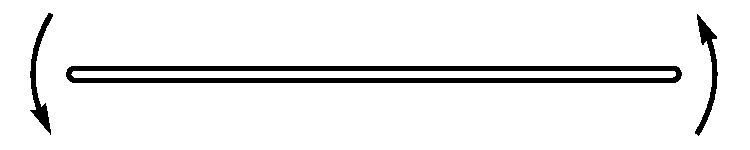
\includegraphics[width=.5\textwidth]{figures/foldedspinningstring.pdf}
\caption{The folded spinning string.}\label{fig:foldedstring}
\end{figure}

The action can now be written as $S= 4\int dt \int_0^R dr {\cal L}$, where ${\cal L}=-T\sqrt{1-r^2\omega^2}$ is the Lagrangian density, and $R,\omega$ are dynamical variables. Demanding that the action is stationary with respect to $R$ then determines $R = 1/\omega$, i.e. the ends of the string move at the speed of light. The energy $E$ and the angular momentum $J$ of the string, given in the canonical formalism by the Hamiltonian and the canonical momentum conjugate to $\theta$ respectively, evaluate to
\ie{}
& E = 4 T \int_0^R {dr\over \sqrt{1-r^2 \omega^2}} = {2\pi T\over \omega},
\\
& J = 4T \int_0^R dr {r^2\omega\over \sqrt{1-r^2\omega^2}} = {\pi T\over \omega^2}.
\fe
It follows that $E$ and $J$ obey
\ie\label{regge}
E^2 = 4\pi T J.
\fe
The relation (\ref{regge}) is known as the Regge trajectory ``with zero intercept''. Note that a more general rotating string solution, in contrast to (\ref{thetasimpsol}), can have ripples that propagate along the radial direction. This would increase the total energy at given angular momentum, leading to $E^2\geq 4\pi T J$. 

The relevance of the Regge trajectory in the mass/spin relation of hadrons was famously suggested by Chew and Frautschi in 1961 based on limited experimental data. While it resembles some crude features of the hadron spectrum in the real world, the relation (\ref{regge}) is expected to hold asymptotically for a family of glueballs in the pure $SU(N)$ Yang-Mills in four dimensions in the limit of large $J$ and $N$, with the string tension $T$ of order $\Lambda^2$.


\subsection{The effective string}
\label{effstrbasic}

It is useful to characterize the geometry of the worldsheet embedding through the induced metric 
\ie\label{inducedh}
h_{ab} \equiv \partial_a X^\mu \partial_b X_\mu.
\fe
The extrinsic curvature of the worldsheet, viewed as a surface embedded in the $D$-dimensional Minkowskian spacetime, is characterized by the second fundamental form
\ie
\Omega_{ab}^\mu = \nabla_a \partial_b X^\mu, 
\fe
where $\nabla_a$ is the covariant derivative with respect to the induced metric (\ref{inducedh}). Note that $\Omega_{ab}^\mu$ is a symmetric tensor with respect to the worldsheet indices $(ab)$, and as a vector in the Minkowskian spacetime is orthogonal to the worldsheet.\footnote{This follows from the explicit expression $\nabla_a \partial_b X^\mu = \partial_a \partial_b X^\mu - \Gamma_{ab}^c\partial_c X^\mu$, where $\Gamma_{ab}^c$ is the Christoffel symbol built out of the induced metric $h_{ab}$. In particular, $\Omega^\mu_{ab} \partial_c X_\mu=\partial_a\partial_b X^\mu \partial_c X_\mu - \Gamma^d_{ab} h_{cd}={1\over 2}(\partial_a h_{bc} + \partial_b h_{ac} - \partial_c h_{ab}) - \Gamma^c_{ab} h_{cd}=0$.} It further obeys the relation
\ie\label{omegarabcd}
\Omega_{ac}^\mu \Omega_{bd\mu} - \Omega_{ad}^\mu \Omega_{bc\mu} = R_{abcd},
\fe
where $R_{abcd}$ is the Riemann tensor associated with $h_{ab}$. 

The equation of motion that follows from the Nambu-Goto action (\ref{ngmink}) can be expressed simply as
\ie\label{ngeom}
h^{ab} \Omega_{ab}^\mu = 0.
\fe
While the Nambu-Goto action is a universal action that captures long wavelength fluctuations, the true action of a relativistic string may be corrected by additional terms that involve $\Omega_{ab}^\mu$ and become important for short wavelength modes. Assuming locality on the worldsheet, at least in the regime of small extrinsic curvature, such corrections to the Lagrangian density may be organized according to terms of increasing weights, where we assign weight 0 to $\partial_a X^\mu$ and weight 1 to each additional derivative.

The Nambu-Goto action has weight zero. Under the assumption of Poincar\'e symmetry of the target Minkowskian spacetime, the lowest weight possible corrections to the Nambu-Goto action, subject to the worldsheet diffeomorphism gauge invariance, are of the form
\ie\label{weighttwo}
\int d^2\sigma \sqrt{- \det h} \left[ \A_1 (h^{ab}\Omega_{ab}^\mu)^2 + \A_2 h^{ac} h^{bd} \Omega_{ab}^\mu \Omega_{cd\mu} \right].
\fe
%where we have defined $h\equiv \det (h_{ab})$.
Due to (\ref{omegarabcd}), a linear combination of these two terms is proportional to the Euler characteristic
\ie\label{eulcar}
\chi = {1\over 4\pi} \int d^2\sigma \sqrt{-\det h} R.
\fe
(\ref{eulcar}) is well known to be topological in the sense that it is invariant under continuous deformations of $h_{ab}$ or $X^\mu$, and therefore does not affect the equation of motion.\footnote{In fact, (\ref{eulcar}) evaluates to a nontrivial result only for a worldsheet configuration that involve splitting/creation or joining/annihilation of strings.}

Furthermore, any first order deformation of the Nambu-Goto Lagrangian density that is proportional to the LHS of the Nambu-Goto equation of motion (\ref{ngeom}), i.e. of the form $h^{ab} \Omega_{ab}^\mu L_\mu$ for some $L_\mu$, can be removed by a field redefinition of the form $X^\mu \to X^\mu + \delta X^\mu$ with $\delta X^\mu \propto L^\mu$. Such is the case for the first term in (\ref{weighttwo}). Therefore, modulo a field redefinition, (\ref{weighttwo}) does not affect the classical dynamics of a string. The leading nontrivial possible corrections to the Nambu-Goto Lagrangian density are weight 4 terms such as $(\Omega^\mu_{ab} \Omega^{ab}_\mu)^2$ and $(\Omega_{ab}^\mu \Omega^{ab\nu})^2$.

In a quantum theory of relativistic strings, such as that of color flux strings in the four-dimensional $SU(N)$ Yang-Mills at large $N$, we expect the long wavelength fluctuations on a long string to be governed by a worldsheet Wilsonian effective action that takes the form of Nambu-Goto theory corrected by the higher derivative terms as outlined above.

%Before attempting at quantization, let us note that there are a priori reasons to believe that consistent relativistic quantum {\it free} string theories exist, such as that of the color flux tube in $SU(N)$ Yang-Mills theory in the infinite $N$ limit. In a quantum theory, we expect long wavelength excitations of the string to be governed by a Wilsonian effective worldsheet action, which admits a derivative expansion starting from the Nambu-Goto theory as outlined above. %One may alternatively formulate the dynamics of the string in terms of a 1PI effective action that captures the scattering matrix of transverse fluctuations of an (infinitely) long extended string. If the strings can split or join, then the ripples on the string may well leave the string in a scattering process, and the scattering matrix of fluctuations on a long string would not be unitary by itself.

\subsection{Polyakov's formalism}

The classical string mechanics described by the Nambu-Goto action can be equivalently formulated through the Polyakov action \cite{Polyakov:1981rd}
\ie\label{spolya}
S_{\rm P}[g_{ab}, X^\mu] = -{1\over 4\pi \A'} \int d^2\sigma \sqrt{-\det g}\, g^{ab} \partial_a X^\mu \partial_b X_\mu,
\fe
where we have introduced a dynamical metric field $g_{ab}$ on the worldsheet, and written the string tension as $T={1\over 2\pi \A'}$. Here $g^{ab}$ stands for the inverse metric. The equation of motion for $g_{ab}$  amounts to the {\it vanishing} of
\ie\label{tabdef}
T_{ab} \equiv {4\pi\over \sqrt{-g}} {\delta S_{\rm P}\over \delta g^{ab}} =-{1\over \A'}\left[ \partial_a X^\mu \partial_b X_\mu - {1\over 2} g_{ab} g^{cd} \partial_c X^\mu \partial_d X_\mu \right] ,
\fe
which is equivalent to setting
\ie\label{ghidre}
g_{ab}\propto h_{ab} = \partial_a X^\mu \partial_b X_\mu.
\fe
Indeed, upon imposing (\ref{ghidre}), $S_{\rm P}$ reduces to the Nambu-Goto action $S_{\rm NG}$. 
Note that $S_{\rm P}$ is invariant with respect to worldsheet diffeomorphism as well as the Weyl transformation $g_{ab}\to e^{2\omega(\sigma)} g_{ab}$. Equivalence with Nambu-Goto theory requires treating both the worldsheet diffeomorphism and the Weyl transformation as {\it gauge} symmetries, so that (\ref{ghidre}) leaves no residual physical degrees of freedom in $g_{ab}$. The $X^\mu$'s are now a set of $D$ {\it free} massless scalar fields propagating in a general worldsheet geometry.

The curvature of a two-dimensional metric $g_{ab}$ is entirely determined by its Ricci scalar $R(g)$, whose Weyl transformation is $R(e^{2\omega} g) = e^{-2\omega} (R(g) - 2\nabla^2\omega)$. Locally it is always possible to find a Weyl transformation that sets $R$ to zero, thereby relating $g_{ab}$ to a flat metric. Furthermore, we can use a combination of Weyl and diffeomorphism gauge transformations to set, at least locally, 
\ie\label{confgaugeflat}
g_{ab}=\eta_{ab}.
\fe
The gauge condition (\ref{confgaugeflat}) is called the {\it conformal gauge}.

In the conformal gauge, the equation of motion for $g_{ab}$, namely
\ie\label{tabzero}
T_{ab}=0,
\fe
is viewed as a set of constraints on $X^\mu$, known as ``Virasoro constraints''. These are supplemented by the equation of motion for $X^\mu$, which can be written as
\ie\label{ppxeqw}
\partial^a \partial_a X^\mu = 0.
\fe
In conclusion, the classical mechanics of the Nambu-Goto string is equivalently characterized, at least locally on the worldsheet, by the dynamical equations (\ref{tabzero}) and (\ref{ppxeqw}). Let us note that despite (\ref{ppxeqw}) taking the form of a free wave equation, the Virasoro constraints (\ref{tabzero}) are nonlinear with respect to $X^\mu$.



%An effective string action beyond Nambu-Goto can also be put in the Polyakov form. In order to maintain diffeomorphism and Weyl gauge symmetries, the higher derivative coupling can be constructed using the exponential of
%\ie
%\varphi \equiv -{1\over 2} \log (g^{ab} \partial_a X^\mu \partial_b X^\mu)
%\fe
%and the Weyl-covariant derivative $\hat \nabla_a$. Acting on a scalar field, $\hat\nabla_a$ would be the same as $%\partial_a$. Acting on a vector field $V^b$, on the other hand, we have
%\ie
%\hat\nabla_a V^b \equiv \nabla_a V^b - \partial_a \varphi \, V^b + \partial^b \varphi\, V_a - \delta_a^b \partial_c \varphi %V^c.
%\fe


\subsection{A first attempt at quantization}
\label{firstattempt}

One may attempt to construct a quantum theory of strings by promoting the Polyakov action principle (\ref{spolya}) to a path integral of the form
\ie\label{zpath}
Z = {1\over {\rm vol}({\cal G})} \int [Dg_{ab} DX^\mu] \, e^{-S_{\rm P}^E [g_{ab}, X^\mu]}.
\fe
For convenience, we have adopted the Euclidean convention, namely that the worldsheet metric $g_{ab}$ is assumed to be of Euclidean signature, and $S_P^E$ is the Euclidean version of Polyakov's action, given by\footnote{Henceforth we will often omit the superscript $E$ for the Euclidean action when there is no room for confusion.}
\ie
S^E_P = {1\over 4\pi \A'} \int d^2\sigma \sqrt{\det g}\, g^{ab} \partial_a X^\mu \partial_b X_\mu.
\fe 
This is so that the functional integral formally converges (modulo gauge redundancy and UV regularization) and we will not need to worry about operator ordering in correlation functions. The relevant Lorentzian observables can be recovered by analytic continuation when needed. The path integral should be normalized by removing the gauge redundancy, formally represented as division by the volume of the (infinite dimensional) group ${\cal G}$ of gauge transformations, namely diffeomorphism and Weyl transformations, in (\ref{zpath}). A more precise construction of the path integral is based on gauge fixing through the Faddeev-Popov procedure, as follows.

We will work with a slightly generalized version of the conformal gauge, setting 
\ie\label{bosconfgaug}
g_{ab} = \hat g_{ab}
\fe
for a suitably chosen {\it fiducial metric} $\hat g_{ab}$ on the worldsheet. Locally, this gauge condition can be reached by a combination of diffeomorphism and Weyl transformation for any non-degenerate $\hat g_{ab}$. The global issues with the conformal gauge will be addressed in section \ref{stringscatt}.

Under an infinitesimal diffeomorphism generated by a vector field $\delta v^a$, combined with an infinitesimal Weyl transformation parameterized by a function $\delta\omega$, the metric $g_{ab}$ transforms by
\ie\label{diffweag}
\delta g_{ab} = -\nabla_a \delta v_b - \nabla_b \delta v_a + 2\delta\omega g_{ab}.
\fe
The gauge fixed form of (\ref{zpath}) can be written as a functional integral over the scalar fields $X^\mu$ in the background fiducial metric $\hat g_{ab}$,
\ie\label{polpath}
Z_{\hat g} = \int [DX^\mu]_{\hat g} \Delta_{\rm FP}[\hat g_{ab}]\, e^{-S^E_{\rm P}[ \hat g_{ab}, X^\mu]},
\fe
where $\Delta_{\rm FP}[\hat g_{ab}]$ is the Faddeev-Popov determinant,
\ie\label{fpdetearl}
& \Delta_{\rm FP}[\hat g_{ab}] = \int [D \widetilde b_{ab} D c^a D \zeta]_{\hat  g} \, e^{-S^E_{\rm gh}[\hat  g, \widetilde b, c, \zeta]},
\\
& S^E_{\rm gh}[\hat  g, \widetilde b,c,\zeta] = {1\over 4\pi} \int d^2\sigma \sqrt{\det\hat g} \,\widetilde b_{ab}(\hat\nabla^a c^b + \hat\nabla^b c^a - 2 \hat g^{ab} \zeta).
\fe
Here $\widetilde b_{ab}$, $c^a$ and $\zeta$ are anti-commuting fields known as Faddeev-Popov ghosts. In particular, $c^a$ and $\zeta$ carry the same tensor index structure as the gauge parameters $\delta v^a$ and $\delta\omega$, whereas $\widetilde b_{ab}$ carries the same index structure as that of the stress-energy tensor. $\hat\nabla_a$ is the covariant derivative with respect to the fiducial metric $\hat  g$. The ghost action $S_{\rm gh}^E$ is derived from (\ref{diffweag}) following the general recipe of section \ref{sec:brstinit}. %The functional integral measure $[DX^\mu]_{\hat g}$ etc. are defined with a suitable UV regularization scheme that is covariant with respect to the fiducial metric.

Note that $\zeta$ serves as a Lagrange multiplier and can be integrated out. This results in a slightly simplified ghost functional integral
\ie
\Delta_{\rm FP}[\hat g_{ab}] = \int [D  b_{ab} D c^a]_{\hat  g} \, e^{-S_{\rm gh}[ \hat  g, b, c ]},~~~ S^E_{\rm gh}[ \hat  g, b,c] = {1\over 2\pi} \int d^2\sigma \sqrt{\det \hat g} \, b_{ab}\hat\nabla^a c^b ,
\fe
where $b_{ab}$ is an anti-commuting symmetric tensor field that is constrained to be traceless, i.e. $\hat g^{ab} b_{ab}\equiv 0$.

Consistency of the gauge fixing requires $Z_{\hat  g}$ to be invariant under formal gauge transformations of $\hat  g$, or more precisely gauge transformations of the gauge fixing condition $g_{ab}=\hat g_{ab}$ (as $\hat g$ is not a dynamical field). While the actions $S_{\rm P}[\hat g, X]$ and $S_{\rm gh}[\hat  g, b,c]$ are indeed diffeomorphism and Weyl invariant (with the understanding that $\hat g$ is transformed accordingly), it is not obvious that the measure $[D X^\mu D b_{ab} D c^a]_{\hat  g}$, which is typically defined with a suitable UV regularization scheme, would be invariant. 

It is indeed possible to construct a diffeomorphism invariant measure $[D X^\mu D b_{ab} D c^a]_{\hat  g}$.\footnote{This amounts to the absence of gravitational anomaly.} For instance, one may expand the field $X^\mu$ over an orthonormal basis of eigenfunctions with respect to the scalar Laplacian in the metric $\hat g$, and define $[DX^\mu]_{\hat g}$ as that of integration over the coefficient variables with a UV cutoff on the eigenvalues. However, the measure generally cannot be made Weyl invariant. An important result derived in Appendix \ref{weylanomalsec} is that under $\hat g_{ab} \to e^{2\omega}\hat  g_{ab}$, $Z_{\hat  g}$ transforms by
\ie\label{weylzz}
Z_{e^{2\omega}\hat  g} = Z_{\hat  g} \exp\left\{ {D-26\over 24\pi} \int d^2\sigma \sqrt{\det \hat  g} \left[\hat  g^{ab} \partial_a \omega \partial_b\omega + \omega R(\hat g) \right] \right\},
\fe
where $D$ is the target Minkowskian spacetime dimension, i.e. the total number of $X^\mu$ fields, and $R(\hat g)$ is the Ricci scalar of the fiducial metric. 

According to (\ref{weylzz}), $Z_{\hat  g}$ is Weyl invariant if and only if $D=26$. It is only in this case that the path integral quantization in the conformal gauge respects the gauge invariance of the classical Polyakov action. This gives rise to the {\it critical bosonic string theory}, whose worldsheet description involves the free quantum field theory of 26 massless scalar fields $X^\mu$ and the ghost fields $b_{ab}, c^a$.

If $D\not = 26$, the ``anomalous'' transformation (\ref{weylzz}) indicates that Weyl invariance does not hold at the quantum level. Either we must accept that the Weyl mode of the worldsheet metric is a dynamical field rather than a gauge redundancy, which amounts to an extra dimension in the target space, or we must modify the Polyakov action in some way so as to cancel the Weyl anomaly. The former option leads to the so-called noncritical string theory. The latter option would be the natural choice if we insist that the string propagates in the $D$-dimensional Minkowskian spacetime. Indeed, one could add to $S_{\rm P}$ the ``composite Liouville action"
\ie\label{compositeliouville}
S_{\rm CL}^E[ g_{ab}, \varphi] = {26-D\over 24\pi} \int d^2\sigma \sqrt{\det g} \left[  g^{ab} \partial_a \varphi \partial_b\varphi - \varphi R( g) \right],
\fe
where $\varphi$ is any scalar field operator constructed out of $X^\mu$ and $ g_{ab}$ that transforms as
\ie
\varphi \to \varphi + \omega
\fe
under the Weyl transformation $g_{ab} \to e^{2\omega} g_{ab}$, so that $e^{-S_{\rm CL}}$ transforms by a factor that precisely cancels against (\ref{weylzz}).
The simplest such choice of $\varphi$ is
\ie
\varphi = -{1\over 2} \log( g^{ab} \partial_a X^\mu \partial_b X_\mu).
\fe
Formally, the gauge fixed path integral
\ie
Z = \int [DX^\mu ]_{\hat  g} \, \Delta_{\rm FP}\, e^{-S_{\rm P} - S_{\rm CL}}
\fe
is Weyl invariant. However, the action $S_{\rm P} + S_{\rm CL}$ is highly non-renormalizable and must be supplemented with higher-derivative counter terms that are not a priori fixed by symmetry principles. % If such a UV complete quantum field theory on the worldsheet exists, which is by no means evident, it should admit $S_{\rm P}+S_{\rm CL}$ as a long-wavelength effective action.



It is interesting to inspect the dynamical consequence of (\ref{compositeliouville}). In the conformal gauge $g_{ab} = \eta_{ab}$, the Lorentzian version of the composite Liouville action can be written as
\ie
S_{\rm CL} = -{26-D\over 24\pi} \int d^2\sigma {(\partial_a \partial_b X^\mu \partial^b X_\mu) (\partial^a \partial_c X^\nu \partial^c X_\nu) \over (\partial_d X^\rho \partial^d X_\rho)^2 }.
\fe
A static long string extending in $X^1$ direction can be described by the classical field configuration $X^0=\tau$, $X^1=\sigma$,\footnote{This field configuration is viewed as a solution to the equation of motion in the conformal gauge, not to be confused with the static gauge condition considered in section \ref{sec:nambugoto}.} with the other components $X^i$ set to zero, $i=2,\cdots, D-1$. Expanding around this configuration, we can write
\ie\label{slqua}
S_{\rm CL} =  -{26-D\over 96\pi} \int d^2\sigma (\partial_a \partial_b X^i \partial^b X^i) (\partial^a \partial_c X^j \partial^c X^j)+ \cdots,
\fe
where $\cdots$ represents higher derivative terms that involve products of more than four fields. The quartic term exhibited in (\ref{slqua}) makes a nontrivial contribution to the $2\to 2$ S-matrix element of the $X^i$ modes on the long string,
\ie\label{smtrcl}
& {}^{out}\langle k, q_3;\ell, q_4 |i, q_1; j, q_2\rangle^{in} = \delta_{ik}\delta_{j\ell} \delta(q_1^\sigma-q_3^\sigma) \delta(q_2^\sigma-q_4^\sigma)
+ \delta_{i\ell}\delta_{jk} \delta(q_1^\sigma-q_4^\sigma)\delta(q_2^\sigma-q_3^\sigma)
\\
& ~~~~~ + {i\over s} \delta^2(q_1+q_2-q_3-q_4) {(26-D)\A'^2\over 192\pi}  \left( s^3 \delta_{ij}\delta_{k\ell} + t^3 \delta_{ik}\delta_{j\ell} + u^3 \delta_{i\ell}\delta_{jk}\right) + \cdots,
\fe
where $q_i\equiv (q_i^\tau, q_i^\sigma)$ are the momenta of the scattering modes, with $q_i^\tau=|q_i^\sigma|$, and $s= -(q_1+q_2)^2$, $t=-(q_1-q_3)^2$, $u=-(q_1-q_4)^2$ are the Mandelstam variables. Note that the 1+1 dimensional kinematics is such that either $t$ or $u$ vanishes.

\begin{figure}[h!]
\centering
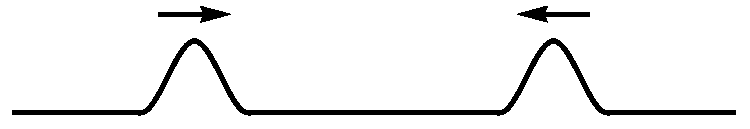
\includegraphics[width=.5\textwidth]{figures/ripplescattering.pdf}
\caption{Scattering of ripples on a long string.}\label{fig:ripples}
\end{figure}

One may be puzzled by how this result could be compatible with the quantization of the Nambu-Goto action in the static gauge, where there is no obvious analog of the composite-Liouville action.\footnote{According to the derivative counting introduced in section \ref{effstrbasic}, the term appearing in (\ref{slqua}) would appear to carry weight 2 , but there exists no weight 2 effective coupling that could be added to the Nambu-Goto action while preserving the target space Poincar\'e symmetry.} A part of the resolution is that in the Nambu-Goto formulation, for $D\not=26$, the interaction term in the S-matrix element (\ref{smtrcl}) arises as a 1-loop contribution.\footnote{To carry out this computation requires employing a UV regularization scheme that respects the target space Poincar\'e symmetry, such as dimensional regularization, and including necessary counter terms. A subtlety is the following: if we take the worldsheet dimension to be $d=2-\epsilon$, the 1-loop amplitude of Nambu-Goto theory would also receive a log divergence proportional to $stu$, which must be canceled by a $d$-dimensional Einstein-Hilbert counter term (which is no longer topological as $d\not=2$). After canceling the divergences, one can then take the $d\to 2$ limit, where the kinematics is such that $stu$ vanishes identically, and recover a finite contribution that is identical to the second line of (\ref{smtrcl}). For further details see Dubovsky, Flauger, Gorbenko, JHEP \textbf{09} (2012), 044 \cite{Dubovsky:2012sh}.} 
Let us further note that in the critical spacetime dimension $D=26$, the worldsheet theory is free in the conformal gauge, whereas the interaction terms in the Nambu-Goto action produce a nontrivial tree-level scattering phase between the fluctuation modes on a long string. This is due to the difference in the notion of worldsheet space and time coordinates between the conformal gauge and the static gauge, which leads to a overall phase difference known as ``gravitational dressing" between the S-matrix elements in the two gauges.



\subsection{Critical string theory}
\label{critbosstr}

Let us now focus on the $D=26$ case, where the gauge-fixed path integral (\ref{polpath}) based on the Polyakov action alone is consistent with the underlying diffeomorphism and Weyl gauge invariance. In principle, the quantum state of a closed string may be described in terms of a wave functional of the fields $X^\mu$, $b_{ab}$, and $c^a$ on a spatial circle of the worldsheet. We will see in Chapter \ref{chap:brst} that not all such states should be regarded physical, and that the precise notion of physical states will be defined in terms of BRST cohomology classes. For now, we will seek an alternative gauge choice in which the ghosts are non-dynamical, so that the physical states can simply be identified with those of the dynamical fields. This can be achieved in the {\it light cone gauge}, defined by 
\ie\label{lcbos}
& \tau = X^+ \equiv {1\over \sqrt{2}}(X^0 + X^1),
\\
& \det g = -1, ~~~  g_{\sigma\sigma} = - g^{\tau\tau}=1.
\fe 
The first condition identifies the worldsheet time $\tau$ with a light-like coordinate $X^+$. The second line provides two more functions worth of conditions that are needed to fix the gauge (almost) completely.

Under the diffeomorphism and Weyl transformation that gave rise to (\ref{diffweag}), the gauge conditions (\ref{lcbos}) vary according to
\ie\label{vargauglicd}
& \delta X^+ = - \delta v^a \partial_a X^+ =-\delta v^\tau ,
\\
& (\det g)^{-1} \delta(\det g) =  g^{ab} \delta g_{ab} = - 2\nabla_a \delta v^a + 4 \delta \omega,
\\
& \delta  g_{\sigma\sigma} = 2 \delta \omega  g_{\sigma\sigma} -2 \nabla_\sigma \delta v_\sigma.
\fe
Following the Faddeev-Popov procedure, the gauge parameters $\delta v^a$ and $\delta\omega$ lead to ghosts $c^a$ and $\eta$, whereas the variations of the gauge conditions (\ref{vargauglicd}) correspond to $b$-type ghosts, which we denote by $b_1, b_2, b_3$. The ghost action that follows from (\ref{vargauglicd}) is 
\ie
S_{\rm gh} = {1\over 4\pi} \int d\tau d\sigma \left( - b_1 c^\tau + b_2 (-2\nabla_a c^a + 4 \eta) + b_3 (2\eta - 2\nabla_\sigma c_\sigma) \right).
\fe 
Integrating out $b_1, b_2$ sets $c^\tau=0$ and $\eta={1\over 2}\nabla_a c^a$. The remaining ghosts $b_3$ and $c^\sigma$ are non-dynamical as their $\tau$-derivatives do not appear in the action. We conclude that the ghost fields play no role in the light cone gauge. After imposing (\ref{lcbos}), the Polyakov action can be expressed as
\ie\label{polyloighcon}
S_{\rm P} = -{1\over 4\pi\A'} \int d\tau d\sigma  \left(- 2 g^{\tau a} \partial_a X^- +  g^{ab}\partial_a X^i \partial_b X^i \right),
\fe
where $X^-\equiv {1\over \sqrt{2}}(X^0-X^1)$, and the index $i$ is summed from 2 to $D-1$. %Note that $ g^{\tau a}$ for $a=\tau,\sigma$ determine $ g^{\sigma\sigma}$ through the gauge condition $ g=-1$. 

To describe the worldsheet of a closed string, we should take the spatial coordinate $\sigma$ to be a periodic variable. A priori, the periodicity of $\sigma$ has no intrinsic meaning and could be $\tau$-dependent. In the light cone gauge, however, we will see below that the periodicity of $\sigma$ is in fact a conserved quantity. In any case, we can decompose $X^-(\tau,\sigma)$ into its Fourier modes in $\sigma$, and integrate out the nonzero modes  which appear linearly in (\ref{polyloighcon}), setting
\ie\label{gtxze}
\partial_\sigma  g^{\tau\sigma} = 0.
\fe
Note that the light cone gauge condition (\ref{lcbos}) still leaves a residual unfixed gauge transformation, namely a diffeomorphism $(\sigma,\tau)\mapsto (\sigma',\tau')$ with
\ie\label{sigmatautran}
\sigma' = \sigma + f(\tau),~~~ \tau' = \tau.
\fe
This transformation can now be used to set $g^{\tau\sigma}$, already made $\sigma$-independent by (\ref{gtxze}), to zero. This leaves (\ref{sigmatautran}) with $f(\tau)=const$ as the only residual gauge redundancy. The light cone gauge condition (\ref{lcbos}) combined with $g^{\tau\sigma}=0$ now determines $g_{ab} = \eta_{ab}$.

From the worldsheet standpoint, the spacetime translation symmetry amounts to the shift symmetry in $X^\mu$, whose associated Noether current is
\ie
j_a^\mu = {1\over 2\pi \A'} \partial_a X^\mu.
\fe
The corresponding conserved charge 
\ie
p^\mu = \oint d\sigma j_\tau^\mu
\fe
is the spacetime momentum of the string. In particular, it follows from the identification $X^+=\tau$ that
\ie\label{pplus}
p^+ = {1\over 2\pi\A'}\oint d\sigma.
\fe
Namely, the lightcone momentum $p^+$ is equal to the circumference $\ell=\oint d\sigma$ of the string in the light cone gauge multiplied by the string tension $T={1\over 2\pi\A'}$.
In addition,  
\ie\label{pminush}
p^- &=-p_+ = {1\over 2\pi \A'}\oint d\sigma \partial_\tau X^- 
\\
&= {1\over 4\pi \A'} \oint d\sigma \left[ (\partial_\tau X^i)^2 +  (\partial_\sigma X^i)^2 \right]
\fe
where the equality in the second line follows from the equation of motion for $ g^{\tau\tau}$,\footnote{As $g^{\tau\tau}$ is fixed by the light cone gauge condition, the equation of motion for $ g^{\tau\tau}$ is viewed as a constraint in the classical theory, or a BRST-exact operator, whose expectation values in all physical states vanish, in the quantum theory.} 
coincides with the worldsheet Hamiltonian in the light cone gauge.

%The zeroth Fourier mode of $X^-$ in $\sigma$ is canonically conjugate to Note that this agrees with $j_a^\mu = {1\over 2\pi \A'} \partial_a X^\mu$ being the worldsheet Noether current associated with target spacetime translation symmetry, and the corresponding conserved charge $p^\mu = \oint d\sigma j_\tau^\mu$ is the spacetime momentum. The Noether charge associated with translation in $X^+$, in particular, is given by

The Hilbert space of a single closed string can now be constructed as that of the $D-2$ free bosons $X^i$, subject to the aforementioned residual diffeomorphism gauge redundancy of {\it constant} shift in $\sigma$. This gauge redundancy should be implemented as a further restriction on the quantum states, namely all {\it physical} states must be invariant with respect to the translation symmetry in $\sigma$. That is, all physical states of the closed string must carry zero total {\it worldsheet} momentum. 

The Hilbert space of the free massless scalar fields $X^i$ on the $\sigma$-circle is spanned by Fock basis states of the form
\ie\label{focks}
|p^i; \{n_k^i, \widetilde n_k^i\}_{k\geq 1}\rangle,
\fe
where $n_k^i$ is the number of massless quanta of $X^i$ that carry $k$ units of momenta each around the circle, and $\widetilde n_k^i$ is the number of quanta that carry $-k$ units of momenta. $p^i$ is the spacetime momentum in the $X^i$-direction, related to the time-derivative of the zeroth Fourier mode of $X^i$ via
\ie
p^i = {1\over 2\pi \A'} \oint d\sigma \partial_\tau X^i.
\fe
The worldsheet Hamiltonian (\ref{pminush}) evaluates to
\ie\label{massrel}
p^- = {(p^i)^2\over 2p^+} + {1\over \A' p^+} \left[ \sum_{i=2}^{D-1} \sum_{k\geq 1} k (n_k^i + \widetilde n_k^i) + A \right],
\fe
where we have used the relation (\ref{pplus}), and have included a normal-ordering constant $A$ that appears in the ground state energy 
\ie
E_0 = {2\pi A\over \ell}
\fe 
of the free scalar field theory on a circle of circumference $\ell$. A priori, the value of $A$ depends on the regularization scheme used in defining the Hamiltonian (\ref{pminush}) as a quantum operator. (\ref{massrel}) can be viewed as the dispersion relation of a particle propagating in the $D$-dimensional Minkowskian spacetime. Lorentz invariance requires such a dispersion to take the form $p^\mu p_\mu + m^2=0$ for some mass $m$ that is independent of $p^\mu$. It follows that $A$ must be independent of $\ell$, and that $E_0$ is a Casimir energy that is free from local counter term ambiguities. This Casimir energy can be calculated either by summing up zero point energy of the oscillator modes of $X^i$ and subtracting UV divergence as dictated by the structure of possible local counter terms, or more elegantly through the conformal transformation property of the stress-energy tensor (Appendix \ref{virasorosec}), giving the result $A=-{D-2\over 12}$.

The residual gauge constraint, namely the vanishing of the total worldsheet momentum, can be expressed as the {\it level-matching condition}
\ie\label{nzeroconsta}
N \equiv \sum_{i=2}^{D-1} \sum_{k\geq 1} k n_k^i = \sum_{i=2}^{D-1} \sum_{k\geq 1}k \widetilde n_k^i .
\fe
The non-negative integer $N$ will be referred to as the (oscillator) level of the state. (\ref{massrel}) is then equivalent to the mass-shell relation $p^\mu p_\mu + m^2=0$, with
\ie\label{dispeac}
m^2 = {4\over \A'} \left(N-{D-2\over 24}\right).
\fe
That is, a closed string state (\ref{focks}) subject to the level-matching condition (\ref{nzeroconsta}) is that of a particle carrying energy-momentum $p^\mu$ in the $D$-dimensional Minkowskian spacetime, whose mass $m$ is given by (\ref{dispeac}). 

We have yet to inspect how the internal degrees of freedom of the string states transform under Lorentz symmetry. This is not at all obvious, as only an $SO(D-2)$ subgroup of the $SO(1,D-1)$ Lorentz group is manifest in the light cone gauge. In particular, the Lorentz generators $J^{i+}, J^{i-}, J^{+-}$ do not correspond to any obvious symmetry transformations on the free scalar fields $X^i$. A related issue is that in the light cone gauge approach thus far we have not used the assumption $D=26$, which would be essential for the equivalence with the conformal gauge formulation in which the spacetime Lorentz invariance is manifest. For $D\not=26$, it turns out that the Weyl anomaly manifests itself in the light cone gauge as a Lorentz anomaly. In this case, one can verify that candidate Lorentz generators $J^{i-}$ built out of the $X^i$'s cannot satisfy the Lorentz algebra relation $[J^{i-}, J^{j-}]=0$.

We can diagnose the Lorentz anomaly more simply by inspecting the level $N=1$ states, which according to (\ref{focks}) involve the excitation of a pair of quanta for $X^i$ and $X^j$, carrying $-1$ and $1$ unit of momentum respectively, for $i,j=2,\cdots, D-1$. The $X^i$'s transform in the vector representation $\mathfrak{v}$ of $SO(D-2)$. Restricting to the case of vanishing transverse momentum, i.e. $p^i=0$, the level 1 states transform in the tensor representation $\mathfrak{v}\otimes \mathfrak{v}$ of the $SO(D-2)$. If $D\not=26$, the $N=1$ states have nonzero mass $m$ according to (\ref{dispeac}), and by Lorentz symmetry must organize into a representation of the massive little group $SO(D-1)$ that contains the $SO(D-2)$ as a subgroup. However, there exists no representation of $SO(D-1)$ that reduces to $\mathfrak{v}\otimes \mathfrak{v}$ with respect to its $SO(D-2)$ subgroup, a contradiction. Therefore, the content of level 1 states can be compatible with the $D$-dimensional Lorentz symmetry only if their mass $m$ vanishes, which by (\ref{dispeac}) requires $D=26$.

An immediate issue with the $D=26$ critical bosonic string theory is the presence of a tachyon state at level $N=0$, whose mass squared $m^2$ is negative. This signifies an instability of the vacuum and the breakdown of quantum perturbation theory for interacting strings. It will turn out that the bosonic string theory admits other, Lorentz non-invariant, backgrounds that are free of such instability (section \ref{conesec}). Regardless, the critical bosonic string theory will serve as a useful starting point for formulating the scattering theory of strings.




\newpage

\section{Quantization of the bosonic string}
\label{chap:brst}

\subsection{BRST quantization}
\label{sec:brstinit}

The Becchi-Rouet-Stora-Tyutin (BRST) formalism is a prescription for constructing a consistent quantum gauge theory based on the gauge-fixed path integral with Faddeev-Popov ghosts. The essential idea is that the notion of gauge invariance of a classical action is replaced by a fermionic nilpotent global symmetry known as the BRST symmetry. The introduction of ghosts in the path integral formally enlarges the space of quantum states. One then demands the physical states to be those that are invariant with respect to the BRST symmetry, and identifies the physical Hilbert space with the space of BRST cohomology.

We begin with the action $S[\phi]$ of a classical gauge theory, where $\phi$ collectively denotes all fields, that is invariant with respect to infinitesimal gauge transformations of the form 
\ie\label{gaugevar}
\delta\phi = \int d\mu_\A \epsilon^\A \delta_\A\phi \equiv \epsilon^\A \delta_\A\phi.
\fe
Here $\A$ is a continuous label that includes the spacetime coordinates. $d\mu_\A$ is a suitable measure on $\A$-space. The gauge parameter $\epsilon^\A$ can be viewed as a function in $\A$. When there is no room for confusion, the integration sign and measure will be omitted in our notation (a continuous version of Einstein summation convention). The gauge variation $\delta_\A$ acts on composite fields as a differentiation according to Leibniz's rule, and obeys an (infinite dimensional) Lie algebra commutation relation
\ie{}
[\delta_\A, \delta_\B] = f_{\A\B}{}^\C \delta_\C,
\fe
where the structure constants $f_{\A\B}{}^\C$ are assumed to be field independent.

As an example, suppose the gauge symmetry of interest is diffeomorphism. In this case, the gauge parameter $\epsilon^\A$ is a vector field $\varepsilon^\mu(x)$, and in particular the label $\A\equiv (x,\mu)$ consists of a spacetime coordinate $x$ together with a vector index $\mu$. We can take the measure on $\A$-space to be the volume form $d\mu_\A=d^dy$, and the integration in $\A$ to include summation over the index $\rho$. A scalar field $\varphi$ transforms under infinitesimal diffeomorphism as $\delta \varphi(x) = -\varepsilon^\rho(x)\partial_\rho \varphi(x)$. In the notation of (\ref{gaugevar}), this amounts to
\ie
\delta_{(y, \rho)} \varphi(x) = - \delta^d(x-y) \partial_\rho \varphi(x).
\fe
The commutator of a pair of diffeomorphisms acts on $\varphi$ as
\ie{}
[\delta_{(y,\rho)}, \delta_{(z,\sigma)}] \varphi(x) &= \delta^d(x-z) \partial_{x^\sigma} \left[ \delta^d(x-y) \partial_\rho\varphi(x) \right] - (y,\rho\leftrightarrow z,\sigma)
\\
&= \int d^dw \left[ -\delta_\rho^\nu \delta^d(w-z)\partial_\sigma\delta^d(x-y) + \delta_\sigma^\nu \delta^d(w-y)\partial_\rho\delta^d(x-z)  \right] \delta_{(w,\nu)}\varphi(x),
\fe
from which we deduce the structure constants of the diffeomorphism algebra,
\ie
f_{(y,\rho) (z,\sigma)}{}^{(w,\nu)} = -\delta_\rho^\nu \delta^d(w-z)\partial_\sigma\delta^d(x-y) + \delta_\sigma^\nu \delta^d(w-y)\partial_\rho\delta^d(x-z) .
\fe

To formulate the gauge theory path integral, we will remove the gauge redundancy by selecting a field configuration in each gauge orbit by imposing the gauge-fixing condition $F^A[\phi]=0$. Here $A$ is a continuous label that loosely speaking has the same number of degrees of freedom as the index $\A$ that labels gauge transformations. The gauge-fixed path integral takes the form (Appendix \ref{sec:fpderiv})
\ie\label{zfix}
Z = \int [D\phi]\, \delta(F^A[\phi]) \det(\delta_\A F^A[\phi]) e^{-S[\phi]},
\fe
where $\delta(\cdots)$ stands for the delta functional and $\det$ stands for a functional determinant. %both of which are typically defined through a regularization scheme that makes the $\A$-space finite-dimensional.
We will assume $F^A[\phi]$ is chosen such that the functional Jacobian $\delta_\A F^A[\phi]$ is non-degenerate. We can write (\ref{zfix}) as a more conventional path integral by expressing both the delta functional and the functional determinant as integration over auxiliary fields,
\ie\label{bfix}
Z = \int [D\phi DB_A D b_A D c^\A] \exp\left\{ -S[\phi] +  i B_A F^A[\phi] - b_A c^\A \delta_\A F^A[\phi]  \right\}.
\fe
Here $b_A$, $c^\A$ are a pair of anti-commuting (field) variables known as Faddeev-Popov ghosts, their respective measure defined via Grassmann/Berezin integration, whereas $B_A$ is a commuting (field) variable that plays the role of Lagrange multiplier.

The gauge-fixed path integral (\ref{bfix}), by construction, is no longer invariant under the gauge transformation of $\phi$. In fact, the notion of gauge invariance is replaced by a fermionic global symmetry $\delta_B$, known as BRST symmetry, that acts on the fields according to
\ie\label{brsttransf}
& \delta_B \phi = -i \epsilon c^\A \delta_\A\phi,
\\
& \delta_B B_A = 0,
\\
& \delta_B b_A = \epsilon B_A,
\\
& \delta_B c^\A = {i\over 2} \epsilon f_{\B\C}{}^\A c^\B c^\C,
\fe 
where $\epsilon$ is a Grassmann-odd parameter. Given any functional ${\cal F}$ of the fields, we will write 
\ie
\delta_B {\cal F} \equiv i \epsilon \mathbb{Q}_B {\cal F},
\fe
where $\mathbb{Q}_B$ is viewed as a derivation. In particular, the BRST transformation of $\phi$ resembles a gauge transformation but with the gauge parameter replaced by the $c$-ghost. Additional key properties of BRST symmetry are 
\ie\label{nilpoedel}
\mathbb{Q}_B^2=0,
\fe
as one can directly verify from (\ref{brsttransf}), and
\ie\label{bfatrans}
i B_A F^A[\phi] - b_A c^\A\delta_\A F^A[\phi] = - \mathbb{Q}_B \left( b_A F^A[\phi] \right).
\fe
The gauge invariance of the original ``matter'' action $S[\phi]$ implies $\delta_B S[\phi]=0$. It then follows from (\ref{bfatrans}) and (\ref{nilpoedel}) that the full ``matter+ghost'' action appearing in (\ref{bfix}) is BRST invariant.

As is the case for any continuous global symmetry, the BRST symmetry is associated with a (fermionic) Noether current $j_B$. The corresponding Noether charge $Q_B$, called the BRST charge, is such that 
\ie
\mathbb{Q}_B\cdot {\cal F} = \{ Q_B, {\cal F} \}^{\rm P}, 
\fe
where $\{\cdot,\cdot\}^{\rm P}$ stands for the Poisson bracket. If we assume that the functional measure in (\ref{bfix}) is also BRST invariant,\footnote{This assumption amounts to the absence of BRST anomaly, which will be analyzed in section \ref{brstwssec}.} then $Q_B$ can be promoted to an operator in the quantum theory that obeys 
\ie
Q_B^2=0.
\fe

A quantum state may be described by a wave functional $\Psi[\phi^{(0)}, c^{(0)}]$, whose arguments are the matter and ghost field configuration at a given instant of time, or more precisely, canonical coordinates on the phase space of the matter+ghost system.\footnote{For the matter field $\phi$ with 2-derivative kinetic term, the corresponding canonical coordinates are $\phi|_{\tau=0} = \phi^{(0)}$. For the ghost system with 1-derivative kinetic term, one may take the canonical coordinates to be $c^\A$ at $\tau=0$ (see Appendix \ref{sec:grassmannpathint} and the footnote around (\ref{updownbcst})).} A {\it physical} state $|\Psi\rangle$ is defined as one that is BRST-invariant, or BRST-closed, namely 
\ie
Q_B|\Psi\rangle=0.
\fe
If the state $|\Psi\rangle$ at time zero can be prepared by a path integral with operator insertion over negative Euclidean time $\tau<0$, of the schematic form
\ie
\Psi[\phi^{(0)}, c^{(0)}] = \int_{(\phi,c)|_{\tau=0}=(\phi^{(0)},c^{(0)})} [D\phi Db Dc]_{\tau<0}\, e^{-S[\phi] - \mathbb{Q}_B(b_A F^A)} {\cal O}[\phi,b,c]
\fe
for some functional ${\cal O}$ of $(\phi, b, c)$ at $\tau<0$, then the wave functional of the state $Q_B|\Psi\rangle\equiv |Q_B \Psi\rangle$ is given by
\ie
{Q}_B\Psi[\phi^{(0)}, c^{(0)}] = \int_{(\phi,c)|_{\tau=0}=(\phi^{(0)},c^{(0)})} [D\phi Db Dc]_{\tau<0}\, e^{-S[\phi] -\mathbb{Q}_B(b_A F^A)} \mathbb{Q}_B {\cal O}[\phi,b,c].
\fe
%In terms of the wave functional $\Psi[\phi,\cdots]$, this condition amounts to\footnote{Here we glossed over the possibility that $\delta_B\phi$ contains time-derivatives, in which case the time-derivatives of fields should be re-expressed in terms of the canonical momenta acting on the wave functionals as appropriate functional derivatives. Alternatively, we may simply work with wave functionals produced by path integral over half of spacetime with insertions of BRST-invariant operators.}
%\ie
%Q_B \Psi[\phi,\cdots] \equiv - i\delta_B \Psi[\phi,\cdots]=0.
%\fe
An essential result is that the transition amplitude between a pair of physical states $|\Psi_i\rangle$ and $|\Psi_f\rangle$, namely
\ie
\langle \Psi_f| U_{fi} | \Psi_i\rangle = \int [D\phi Db Dc]_{\tau_i\leq \tau\leq \tau_f} \,\Psi_f^*[\phi_f,c_f] e^{-S[\phi] - \mathbb{Q}_B(b_A F^A)} \Psi_i[\phi_i,c_i] ,
\fe
is invariant under deformations of the gauge condition $F^A[\phi]=0$. Here the time evolution operator $U_{fi}$ is represented by the path integral over field configurations on a time interval $[\tau_i, \tau_f]$, subject to boundary conditions $(\phi,c)|_{\tau=\tau_i}=(\phi_i,c_i)$ and $(\phi,c)|_{\tau=\tau_f}=(\phi_f,c_f)$. The matrix element is obtained by further integrating against the wave functionals $\Psi_i[\phi_i,c_i]$ and $\Psi_f^*[\phi_f,c_f]$. Indeed, under an arbitrary small change of the gauge condition, $F^A\to F^A + \delta' F^A$, the transition amplitude changes by
\ie\label{brstvaramp}
\delta' \langle \Psi_f| U_{fi} | \Psi_i\rangle = - \int [D\phi Db Dc]_{\tau_i\leq \tau\leq \tau_f}  \,\Psi_f^*[\phi_f,c_f] e^{-S[\phi] - \mathbb{Q}_B(b_A F^A)} \mathbb{Q}_B(b_A \delta' F^A) \Psi_i[\phi_i,c_i] .
\fe
Note that the notion of Hermitian conjugate state, or the complex conjugation of the wave functional, is defined such that $Q_B$ is a Hermitian operator.
Provided that the wave functionals in question are BRST invariant, the integrand on the RHS of (\ref{brstvaramp}) can be written as a total BRST variation, which then integrates to zero (assuming the BRST invariance of the measure).

Furthermore, shifting a physical state $|\Psi\rangle$ by a BRST-exact state $Q_B|\chi\rangle$ for some $|\chi\rangle$ does not affect transition amplitudes between $|\Psi\rangle$ and any other physical states. Thus we may view $|\Psi\rangle$ as physically equivalent to $|\Psi\rangle+Q_B|\chi\rangle$, and identify the space of physical states with the cohomology of $Q_B$. 

%Moreover, in a unitary gauge theory, there is a notion of Hermitian inner product on the space of states such that $Q_B$ is Hermitian, a BRST-exact state has zero norm (and is hence a null state), whereas a nontrivial BRST-cohomology representative has positive norm.

\subsection{BRST on the worldsheet}
\label{brstwssec}

As already seen in section \ref{firstattempt}, the critical bosonic string theory in the conformal gauge $ g_{ab} = \hat g_{ab}$ is described by the matter+ghost worldsheet action
\ie
S[X^\mu, b_{ab}, c^a] = S_P[\hat g_{ab}, X^\mu] + S_{\rm gh}[\hat g_{ab}, b_{ab}, c^a].
\fe
This follows from the general BRST formalism introduced in section \ref{sec:brstinit} and further integrating out the Lagrange multiplier field $B_{ab}$ and the dynamical metric $g_{ab}$. As the gauge condition is linear in $g_{ab}$, integrating out the latter simply implements the equation of motion that sets $B_{ab}$ to be equal to the stress-energy tensor $T_{ab}$ of the $(X^\mu, b_{ab}, c^a)$ system,
\ie\label{totalstress}
T_{ab} = T_{ab}^X + T_{ab}^{\rm gh}.
\fe
The BRST transformation of the worldsheet fields now takes the form
\ie\label{brsttrnsfbos}
& \delta_B X^\mu = i \epsilon c^a \partial_a X^\mu,
\\
& \delta_B b_{ab} = i \epsilon T_{ab},
\\
& \delta_B c^a = i \epsilon c^b \hat\nabla_b c^a.
\fe
In the quantum theory, the BRST symmetry is more precisely formulated in terms of its Noether current $j^B_a$ as a local operator. We will adopt the Euclidean fiducial metric $\hat g_{ab} = \delta_{ab}$ and work in complex coordinates $(z,\bar z)$.
It will turn out that the holomorphic and anti-holomorphic components of the BRST current, denoted $j^B_{z}\equiv j_B$ and $j^B_{\bar z}\equiv \widetilde j_B$, are independently conserved. The BRST charge can be written as
\ie\label{qbcont}
Q_B = \oint {dz\over 2\pi i} j_B(z) - \oint {d\bar z\over 2\pi i} \widetilde j_B(\bar z),
\fe
where the contour of integration is understood to enclose, in counterclockwise orientation, the operator on which $Q_B$ acts.

To express $j_B(z)$ explicitly in terms of the matter and ghost fields requires introducing a notion of normal ordering, as follows.
It is conventional to denote the nontrivial components of the ghost fields as $b\equiv b_{zz}$, $\widetilde b\equiv b_{\bar z\bar z}$, and $c\equiv c^z$, $\widetilde c\equiv c^{\bar z}$. The OPE between the holomorphic $b$ and $c$ fields, for instance, contains a singular term of the form\footnote{The notation $\sim$ stands for ``equal up to terms that are analytic in $z$''.}
\ie\label{bcintrosing}
b(z) c(0) \sim {1\over z},~~~~ c(z) b(0)\sim {1\over z}.
\fe
The normal-ordered product of ghost fields will be defined by subtracting all possible singular Wick contractions in the product, as described in Appendix \ref{sec:freeboson}, \ref{freeferm}. By convention whenever we write product of fields at one given point, the product is understood to be normal ordered. For instance, $:b(w)c(z): \equiv b(w)c(z) - {1\over w-z}$, and $:b(z) c(z): \equiv \lim_{w\to z} :b(w) b(z):$ will be denoted simply $bc(z)$, and so forth. The $bc$ system by itself is a CFT with holomorphic stress-energy tensor
\ie\label{bcstress}
T^{\rm gh} = - (\partial b) c - 2 b\partial c.
\fe
Note that this expression is unambiguously fixed by the requirement that $b$ and $c$ are conformal primaries, of weight $(2,0)$ and $(-1,0)$ respectively as dictated by their origin from the gauge fixing prescription.  One can further verify that the OPE of $T^{\rm gh}$ with itself is governed by the Virasoro algebra with central charge $c^{\rm gh}=-26$.

We can now write an explicit expression of the holomorphic BRST current
\ie\label{jbexpex}
j_B = c T^X + bc\partial c + {3\over 2} \partial^2c,
\fe
where $T^X = -{1\over \A'}\partial X^\mu \partial X_\mu$ is the stress-energy tensor of the $X^\mu$ CFT of central charge $D$.
The last term on the RHS of (\ref{jbexpex}) is a total derivative and does not contribute to $Q_B$. Nonetheless, it must be included if we demand $j^B$ to transform as a conformal primary, a necessary condition for the BRST symmetry to be non-anomalous on a topologically nontrivial worldsheet. %\footnote{This is similar to the Weyl anomaly analyzed in Appendix \ref{weylanomalsec}.} %Furthermore, even allowing for adding arbitrary total derivatives, one can verify that $j^B$ can be made a conformal primary only if $D=26$. 

As already mentioned, the BRST transformation of the $b$ ghost is the total stress-energy tensor, namely\footnote{In terms of local operators, the notation $Q_B\cdot {\cal O}$ is defined through the contour representation (\ref{qbcont}), where the contour is chosen so as to enclose the support of ${\cal O}$. This is equivalent to $\{Q_B, {\cal O}\}$, when both $Q_B$ and ${\cal O}$ are interpreted as linear operators acting on a suitable space of states.}
\ie\label{qbbtz}
Q_B\cdot b= T = T^X + T^{\rm gh}.
\fe
The nilpotency of $Q_B$ further implies that
\ie
T(z) T(0) = T(z) Q_B\cdot b(0) = Q_B \cdot(T(z) b(0)) 
\fe
can have at most ${1\over z^2}$ singularity, as this is the case for $T(z) b(0)$ OPE. It follows that there is no ${1\over z^4}$ term in the $T(z) T(0)$ OPE, and therefore the total central charge $c=D-26$ must be zero. This is the condition for the absence of BRST anomaly. It is explained in section \ref{weylanomalsec} that the same condition also ensures the cancellation of Weyl anomaly on a curved worldsheet.

In explicit computations it will often be convenient to work with the oscillator representation of the BRST charge,
\ie\label{qosc}
Q_B = \sum_{n\in\mathbb{Z}} c_n L^X_{-n} + \sum_{m,n\in\mathbb{Z}} {m-n\over 2} :c_m c_n b_{-m-n}: - c_0 +  ({\rm anti-holomorphic}),
\fe
where the oscillator modes $b_n=\oint {dz\over 2\pi i} z^{n+1} b(z)$ and $c_n=\oint {dz\over 2\pi i} z^{n-2} c(z)$ obey $\{ b_n, c_m\}=\delta_{n,-m}$ and $\{ b_n, b_m\}=\{ c_n, c_m\}=0$. The normal ordering prescription in (\ref{qosc}) is defined by moving all the positively graded oscillators to the right of the negatively graded ones, multiplied by $-1$ whenever a pair of Grassmann-odd fields are exchanged.\footnote{This normal ordering on oscillator modes is a priori unrelated to the normal ordering prescription on the products of local field operators. It is conventional to group $b_0$ with the positively graded oscillators and $c_0$ with the negatively graded oscillators.} One may directly verify from (\ref{qosc}) that 
\ie
\{Q_B, b_n\} = L_n, 
\fe
where $L_n=\oint {dz\over 2\pi i} z^{n+1} T(z)$ is the Virasoro generator of the total stress-energy tensor (\ref{totalstress}), in agreement with (\ref{qbbtz}).

The space of states, or equivalently the space of local operators by the state/operator map, of the $bc$ ghost system has some unusual properties due to its non-unitary nature and requires some explanation. In the holomorphic sector, local operators can be constructed as normal ordered products of $b$, $c$ and their derivatives. The lowest weight operators are not the identity, but $c$ and $c\partial c$, both of weight $-1$. Under the state/operator map, they correspond to a pair of degenerate ground states, denoted $|\downarrow\rangle$ and $|\uparrow\rangle$, that obey\footnote{In the wave functional formalism of section \ref{sec:brstinit}, the ground states of the $bc$ system are represented by $\Psi_\downarrow[c] \propto \prod_{n=1}^\infty c_n$ and $\Psi_\uparrow[c] \propto \prod_{n=0}^\infty c_n$, where $c_n$ are the Fourier modes of $c(\sigma)$ on the unit circle.}
\ie\label{updownbcst}
& b_0 |\downarrow\rangle = c_0 |\uparrow\rangle = 0,
\\
& c_0|\downarrow\rangle = |\uparrow\rangle,~~~ b_0 |\uparrow\rangle = |\downarrow\rangle.
\fe
Note that the identity operator is mapped to $b_{-1}|\downarrow\rangle$. Combining the holomorphic and anti-holomorphic sectors, we will write $|\downarrow, \downarrow\rangle$ for the state that corresponds to the operator $c\widetilde c(0)$, and so forth. 

The $bc$ system has a $U(1)$ ghost number symmetry that assigns charge (``ghost number") 1 to $c$ and $-1$ to $b$. The corresponding Noether current is 
\ie\label{bcghostcurr}
j_{\rm gh} = - bc.
\fe
While $j_{\rm gh}$ is a conserved current of weight $(1,0)$, it is not a Virasoro primary. Indeed, the OPE of $T^{\rm gh}$ with $j_{\rm gh}$ takes the form
\ie\label{jbctope}
T^{\rm gh}(z) j_{\rm gh}(0) \sim -{3\over z^3} + {1\over z^2} j_{\rm gh}(0)  + {1\over z} \partial j_{\rm gh}(0).
\fe
This leads to an anomaly in the ghost number symmetry on a curved worldsheet, whose implications on correlation functions of the $bc$ system will be discussed in section \ref{sec:bcghost}.



\subsection{Siegel constraint and BRST cohomology}
\label{sec:siegbrst}

The BRST formalism in the conformal gauge identifies the physical states of a closed string with a cohomology class of $Q_B$ on the space ${\cal H}$ of all quantum states of the $(X^\mu, b_{ab}, c^a)$ system. An important subtlety, however, is that the conformal gauge condition on the cylinder still leaves residual gauge redundancies, namely the diffeomorphisms corresponding to constant shifts of the worldsheet coordinates $\sigma^a$. The residual gauge redundancies must be accounted for through further constraints on the physical states. A closer inspection of the equivalence with the light cone gauge (section \ref{brstlighconesec}) indicates that physical string states should obey the 
{\it Siegel constraint}:
\ie\label{siegelbb}
b_0 |\Psi\rangle = \widetilde b_0 |\Psi\rangle = 0.
\fe
In fact, we will see in section \ref{stringscatt} that the Siegel constraint is precisely needed to ensure the perturbative unitarity of the string S-matrix. Furthermore, we will see in Chapter \ref{sftchap} that (\ref{siegelbb}) is naturally interpreted in the Batalin-Vilkovisky formalism of closed string field theory as the combination of a constraint and a gauge condition.

Even though ${\cal H}$ is not quite a Hilbert space, one can define a projector $P_0$ onto the subspace annihilated by $L_0$,\footnote{Strictly speaking, to define such a projector $P_0$ requires either regularizing the target spacetime (parameterized by $X^\mu$) to be of finite volume, or alternatively restricting to the space ${\cal H}_k$ of states with definite spacetime momentum $k^\mu$ as in (\ref{hklrfir}). This subtlety does not affect the conclusion of this section, but will be relevant in section \ref{sec:masslesseffsftbos} and \ref{sec:rollingosft}.} such that $1-P_0$ projects onto a subspace on which $L_0$ is invertible. $Q_B$ commutes with $L_0$ and therefore commutes with $P_0$. Any $Q_B$-closed state $|\Psi\rangle$ can be written as
\ie
|\Psi\rangle &= P_0 |\Psi\rangle + \{Q_B, b_0\} L_0^{-1} (1-P_0) |\Psi\rangle
\\
&= P_0|\Psi\rangle + Q_B  b_0 L_0^{-1} (1-P_0) |\Psi\rangle,
\fe
and represents the same $Q_B$-cohomology class as $P_0|\Psi\rangle$. In other words, every BRST cohomology class admits a zero weight representative. %Note that $Q_B$ anti-commutes with $b_0$ over $P_0{\cal H}$. 
In fact, the Siegel constraint (\ref{siegelbb}) together with $Q_B$-closure imply
\ie\label{levelmat}
L_0 |\Psi\rangle = \widetilde L_0 |\Psi\rangle = 0.
\fe
Let $\widehat{\cal H}$ be the subspace of $P_0{\cal H}$ that obeys Siegel constraint, i.e. the space of states satisfying both (\ref{siegelbb}) and (\ref{levelmat}). The argument above shows that $Q_B$-cohomology subject to Siegel constraint is equivalent to the cohomology of $Q_B$ restricted to $\widehat{\cal H}$.

Suppose the state $|\Psi\rangle$ carries spacetime momentum $k^\mu$, and total left and right oscillator levels $N$ and $\widetilde N$ defined by
\ie\label{nwtnlevels}
& N = \sum_{m=1}^\infty \big( \A_{-m}^\mu \A_{m \mu} + mb_{-m} c_m + mc_{-m} b_m \big),
\\
& \widetilde N = \sum_{m=1}^\infty \big( \widetilde\A_{-m}^\mu \widetilde\A_{m \mu} + m \widetilde b_{-m} \widetilde c_m + m \widetilde c_{-m} \widetilde b_m \big),
\fe
where $\A_n^\mu, \wt \A_n^\mu$ are the oscillators associated with $X^\mu$, defined as in (\ref{kalpx}).
The zero weight condition (\ref{levelmat}) is equivalent to the level-matching property $N=\widetilde N$ together with the dispersion relation
\ie\label{masshe}
{\A'\over 4} k^2 + N - 1 = 0.
\fe
It follows that the mass $m$ of the string state in spacetime is given by
\ie
m^2 = {4\over \A'}(N-1),
\fe
This formula is in formal agreement with the mass spectrum (\ref{dispeac}) found in the light cone gauge, modulo the interpretation of the level $N$ which is not obviously equivalent to that of the light cone gauge states (\ref{nzeroconsta}), and that we have yet to fully take into account the BRST conditions.

As $Q_B$ commutes with the spacetime translation symmetry, it suffices to restrict to the subspace of ${\cal H}$ of definite spacetime momentum $k^\mu$, which we will denote by ${\cal H}_k$.\footnote{Technically, ${\cal H}_k$ is a subspace in the distributional sense of a rigged Hilbert space or Gelfand triple.} The space ${\cal H}_k$ can be constructed by acting on the oscillator ground state $|k, \downarrow, \downarrow\rangle$ with left and right oscillators independently, and therefore can be expressed as
\ie\label{hklrfir}
{\cal H}_k = {\cal H}_k^L\otimes {\cal H}_k^R,
\fe
where ${\cal H}_k^{L/R}$ may be viewed as the space of states built out of left/right oscillators only. The BRST charge can be split as
\ie\label{qbsplit}
Q_B = Q_B^L \otimes 1 + (-)^{F_L}\otimes Q_B^R,
\fe
where $Q_B^{L}, Q_B^R$ act on ${\cal H}_k^{L},{\cal H}_k^R$ respectively, and are separately nilpotent. Here $F_L$ counts the number of Grassmann-odd left oscillators, and is included so that the two terms on the RHS of (\ref{qbsplit}) anti-commute. Moreover, we will write $\widehat{\cal H}_k^{L/R}$ for the zero weight subspace of ${\cal H}_k^{L/R}$ subject to Siegel constraint. It suffices to analyze the BRST cohomology of $Q_B^{L,R}$ on $\widehat{\cal H}_k^{L,R}$ independently, and the full BRST cohomology describing physical string states of momentum $k^\mu$ can be recovered from the tensor product of the left and right sectors.

To begin with, at level $N=0$, the only state in ${\cal H}_k$ that obeys the Siegel constraint is
\ie\label{kdds}
|k, \downarrow, \downarrow\rangle.
\fe
The zero weight condition (\ref{masshe}) leads to $k^2= -m^2 = {4\over \A'}$. Such a state is necessarily $Q_B$-closed and not $Q_B$-exact. Thus, the only nontrivial level 0 BRST cohomology is represented by (\ref{kdds}), corresponding to a tachyon carrying momentum $k^\mu$.

Next, at level $N=1$, the zero weight condition requires $k^\mu$ to be null. The level 1 subspace of $\widehat{\cal H}_k^L$ contains states of ghost number $-1$, 0, or 1. As $Q_B^L$ raises ghost number by 1, it necessarily annihilates the states of ghost number 1, which are of the form $c_{-1}|k,\downarrow\rangle$. On the ghost number $-1$ and 0 states, on the other hand, $Q_B^L$ acts by
\ie{}
& Q_B^L b_{-1} |k, \downarrow\rangle = \sqrt{\A'\over 2} k_\mu \A_{-1}^\mu |k, \downarrow\rangle,
\\
& Q_B^L \A_{-1}^\mu |k, \downarrow\rangle = \sqrt{\A'\over 2} k^\mu c_{-1} |k,\downarrow\rangle.
\fe
Assuming that $k^\mu$ is nonzero, it follows that a general $Q_B^L$-closed level 1 state in $\widehat{\cal H}_k^L$ takes the form
\ie\label{lvlone}
(e_\mu \A^\mu_{-1} + \C c_{-1})|k,\downarrow\rangle,~~~k^\mu e_\mu = 0,
\fe
whereas shifting by a $Q_B^L$-exact state identifies
\ie
& e_\mu \sim e_\mu + \zeta k_\mu,~~\forall \zeta,
\\
& \C\sim 0.
\fe
The resulting cohomology of $Q_B^L$ is represented by states of the form $e_\mu \A_{-1}^\mu|k,\downarrow\rangle$ subject to the transversality condition $k\cdot e =0$ and the identification $e_\mu\sim e_\mu + \zeta k_\mu$. The Lorentz transformation property of such states is identical to that of a massless vector boson. Combining the left and right sectors, we find that the $Q_B$-cohomology at level 1 is represented by states in $\widehat{\cal H}$ of the form
\ie\label{levelonestates}
e_{\mu\nu} \A_{-1}^\mu\widetilde\A_{-1}^\nu |k,\downarrow,\downarrow\rangle,~~~k^2=0,~~~k^\mu e_{\mu\nu}=k^\mu e_{\nu\mu}=0,
\fe
subject to the identification 
\ie\label{gaugezeta}
e_{\mu\nu} \sim e_{\mu\nu} + \zeta_\mu k_\nu + k_\mu\widetilde\zeta_\nu.
\fe

It is useful to examine the Lorentz transformation property of the massless states (\ref{levelonestates}) in a frame in which $k^0=k^1$, and $k^i=0$ for $i=2,\cdots, 25$. In our convention $k^- \equiv {1\over \sqrt{2}} (k^0-k^1)=0$, and the transversality condition on $e_{\mu\nu}$ reduces to
\ie
e_{+\mu} = e_{\mu+} = 0.
\fe
The identification (\ref{gaugezeta}) can be used to set $e_{-\mu}=e_{\mu-}=0$. Therefore, a general level 1 $Q_B$-cohomology class of the said momentum is represented by
\ie
\sum_{i,j=2}^{25} e_{ij} \A^i_{-1} \widetilde\A^j_{-1} |k^+, k^-=k^i=0,\downarrow,\downarrow\rangle.
\fe
These states organize into three irreducible representations with respect to the compact part of the massless little group $SO(24)$, which amount to setting $e_{ij}$ to a symmetric traceless tensor, an anti-symmetric tensor, or $\delta_{ij}$. They are interpreted as the 1-particle states of the graviton, an anti-symmetric rank-2 tensor field known as the ``$B$-field'', and a massless scalar known as the dilaton. %A important fact that is far from obvious is that the expectation value of the dilaton field controls the effective string coupling, as will be explained in section \ref{weylws}.

A direct calculation of the BRST cohomology at higher levels $N\geq 2$ by enumerating the closed and exact states can be a rather tedious exercise. In section \ref{brstlighconesec} and \ref{ocqsec}, we will give a complete characterization of the BRST cohomology by relating the latter to the light cone gauge quantization and the ``old covariant quantization'' respectively.

\subsection{Equivalence to light cone gauge}
\label{brstlighconesec}

To relate the BRST quantization to the light cone gauge, we begin by defining the left-handed ``light cone oscillator number"
\ie
N^{\rm lc} \equiv \sum_{m=1}^\infty {1\over m} \left( \A^+_{-m} \A^-_m - \A^-_{-m} \A^+_m \right),
\fe
where $\A^\pm_m$ are the oscillators associated with $X^\pm \equiv {1\over \sqrt{2}}(X^0\pm X^1)$ and obey $[\A_m^+, \A_n^-] = -m \delta_{m,-n}$. Note that $N^{\rm lc}$ counts the {\it number} (rather than the level) of $\A^-$ excitations minus the number of $\A^+$ excitations. 

Without loss of generality, suppose the light cone momentum $k^+$ is nonzero. The left sector BRST charge $Q_B^L$ can be decomposed according to the grading defined by $N^{\rm lc}$ quantum number 1, 0, or $-1$, as
\ie
Q_B^L = Q_1 + Q_0 + Q_{-1}.
\fe
In particular, $Q_1$ admits a simple expression
\ie
Q_1 = - \sqrt{\A'\over 2} k^+ \sum_{m\not=0} \A_{-m}^- c_m
\fe
and is nilpotent. Next we define a sort of ``conjugate" operator to $Q_1$,
\ie
R_{-1} \equiv \sqrt{2\over \A'}{1\over k^+} \sum_{m\not=0} \A_{-m}^+ b_m,
\fe
which carries $N^{\rm lc}$ quantum number $-1$ as indicated by the subscript, and
\ie{}
& S_0 \equiv \{Q_1, R_{-1}\} ,
\\
& U_{-1} \equiv \{Q_0, R_{-1}\} ,
\\
& V_{-2} \equiv \{Q_{-1}, R_{-1}\} .
\fe
Note that the operator $S_0$, given explicitly by
\ie
S_0 = \sum_{m=1}^\infty \left( - \A^+_{-m} \A^-_m - \A^-_{-m} \A^+_m + mb_{-m} c_m + m c_{-m} b_m \right)  ,
\fe
counts the total level of light cone and ghost oscillators. 

We claim that over the space $\widehat{\cal H}_k^L$, the following statements hold:

\noindent (1) The cohomology of $Q_1$ is isomorphic to the kernel of $S_0$.

\noindent (2) The kernel of $S_0$ is isomorphic to the kernel of $S_0+U_{-1}+V_{-2} = \{Q_B^L, R_{-1}\}$.

\noindent (3) The cohomology of $Q_B^L$ is isomorphic to the kernel of $S_0+U_{-1}+V_{-2}$.




To prove claim (1), first note that $Q_1$ commutes with $S_0$. Suppose a state $|\Psi\rangle$ is in the kernel of $S_0$, then it has no ghost excitation. Due to Siegel constraint $b_0|\Psi\rangle=0$, $|\Psi\rangle$ must be proportional to $|\downarrow\rangle$ in the ghost sector, which has ghost number 1. It follows that $Q_1|\Psi\rangle$ has ghost number 2, but is still annihilated by $S_0$ and by $b_0$. There are no such states, thus $Q_1|\Psi\rangle=0$. Furthermore, a nonzero $|\Psi\rangle$ cannot be $Q_1$-exact and represents a nontrivial $Q_1$-cohomology class, giving an injective map $ {\rm Ker} (S_0)\to {\rm Coh}(Q_1)$.

Going the other way, suppose $Q_1|\Psi\rangle=0$. Without loss of generality, we can assume that $|\Psi\rangle$ is an eigenstate of $S_0$ with eigenvalue $s$. Either $s=0$, i.e. $|\Psi\rangle$ lies in the kernel of $S_0$, or $s\not=0$, in which case we can write
\ie
|\Psi\rangle &= {1\over s} S_0 |\Psi\rangle = {1\over s} \{Q_1, R_{-1}\} |\Psi\rangle = {1\over s} Q_1 R_{-1} |\Psi\rangle,
\fe
and is therefore $Q_1$-exact. This shows that the map ${\rm Ker} (S_0)\to {\rm Coh}(Q_1)$ is also surjective and therefore an isomorphism.

The isomorphism of claim (2) can be constructed explicitly as
\ie\label{isosuv}
 {\rm Ker}(S_0)& \longrightarrow {\rm Ker}(S_0 + U_{-1} + V_{-2})
\\
 |\Psi\rangle &~ \mapsto~ {1\over 1+S_0^{-1}(U_{-1}+V_{-2})} |\Psi\rangle \equiv \sum_{n=0}^\infty (-)^n (S_0^{-1}(U_{-1}+V_{-2}))^n |\Psi\rangle
\fe 
Note that all states in ${\rm Ker}(S_0)$ have $N^{\rm lc}=0$, and so $N^{\rm lc}\leq -1$ on $(U_{-1}+V_{-2})({\rm Ker} S_0)$. It follows that $S_0$ is invertible on $(U_{-1}+V_{-2})({\rm Ker} S_0)$. Furthermore, $N^{\rm lc}\leq -1$ on $S_0^{-1} (U_{-1}+V_{-2})({\rm Ker} S_0)$, and we can iterate this argument to see that $(S_0^{-1}(U_{-1}+V_{-2}))^n$ is well defined on ${\rm Ker}(S_0)$ for all positive integer $n$.\footnote{Note that at any given total oscillator level, the sum over $n$ in (\ref{isosuv}) involves only finitely many nonzero terms.}


To prove (3), first let us establish that the kernel of $S_0 + U_{-1}+V_{-2}$ is $Q_B^L$-closed. Suppose $|\Psi\rangle$ is annihilated by $S_0 + U_{-1} + V_{-2}$. Since $S_0 + U_{-1}+V_{-2}$ commutes with the ghost number, without loss of generality, we can assume that $|\Psi\rangle$ has a definite ghost number. Next, we can decompose 
\ie\label{nlcpsi}
|\Psi\rangle = \sum_{n\leq n_0} |\Psi_n\rangle,
\fe
where the subscript $n$ labels the $N^{\rm lc}$ quantum number.
The maximal $N^{\rm lc}$ component $|\Psi_{n_0}\rangle$ must be annihilated by $S_0$ by itself, which implies that $n_0=0$. It then follows from the Siegel constraint that $|\Psi_0\rangle$, thereby $|\Psi\rangle$, has ghost number 1. Now $Q_B^L|\Psi\rangle$ has ghost number 2, and is also annihilated by $S_0 + U_{-1}+V_{-2}$. The maximal $N^{\rm lc}$ component of $Q_B^L|\Psi\rangle$ must then be annihilated by $S_0$, as well as by $b_0$ (since $Q_B^L$ and $b_0$ anti-commute over $\widehat{\cal H}_k^L$), but there are no such states with ghost number 2. Thus $Q_B^L|\Psi\rangle=0$. A similar argument shows that a nonzero $|\Psi\rangle$ cannot be $Q_B^L$-exact and represents a nontrivial $Q_B^L$-cohomology class, thereby giving an injective map ${\rm Ker}(S_0 + U_{-1} + V_{-2}) \to{\rm Coh}(Q_B^L)$. 

%Together with (1), (2), we now have a map ${\rm Ker}(S_0)\to {\rm Coh}(Q_B^L)$, which is clearly injective by inspecting the maximal $N^{\rm lc}$ component.

Going the other way, suppose $|\Psi\rangle\in\widehat{\cal H}_k^L$ is $Q_B^L$-closed. Applying the decomposition (\ref{nlcpsi}), we have $Q_1 |\Psi_{n_0}\rangle=0$, and therefore by claim (1) can write
\ie\label{recarga}
|\Psi_{n_0}\rangle = |\Phi\rangle + Q_1 |\chi\rangle,
\fe
where $|\Phi\rangle$ is annihilated by $S_0$ and has the same $N^{\rm lc}$ eigenvalue $n_0$ as $|\Psi_{n_0}\rangle$, while $|\chi\rangle$ has $N^{\rm lc}$ eigenvalue $n_0-1$.
The state
\ie
|\Psi'\rangle \equiv {1\over 1+S_0^{-1}(U_{-1}+V_{-2})} |\Phi\rangle,
\fe
which is well-defined by the same argument as that of (\ref{isosuv}), is annihilated by $S_0 + U_{-1}+V_{-2}$ and thus by $Q_B^L$. The difference 
\ie\label{remainder}
&|\Psi\rangle - |\Psi'\rangle - Q_B^L|\chi\rangle 
\\
&= \sum_{n=1}^\infty (-)^{n-1} (S_0^{-1}(U_{-1}+V_{-2}))^n |\Phi\rangle -( Q_0+Q_{-1})|\chi\rangle + \sum_{n\leq n_0-1} |\Psi_n\rangle
\fe
is $Q_B^L$-closed and has maximal $N^{\rm lc}$ quantum number $n_0-1$. In other words, $|\Psi\rangle$ is equal to $|\Psi'\rangle\in {\rm Ker}(S_0+U_{-1}+V_{-2})$, up to a $Q_B^L$-exact state, and up to a $Q_B^L$-closed remainder (\ref{remainder}) that has lower $N^{\rm lc}$ quantum number. Repeating the same procedure to the remainder recursively, we see that $|\Psi\rangle$ can be put in ${\rm Ker}(S_0+U_{-1}+V_{-2})$ up to a $Q_B^L$-exact state, thus completing the proof of claim (3).


It follows from claims (2) and (3) that $Q_B^L$-cohomology classes are in 1-1 correspondence with the states created by acting the transverse oscillators $\A^i_{-m}$, $m\geq 1$, on $|k,\downarrow\rangle$. Combined with the right sector, this shows that the $Q_B$-cohomology classes subject to Siegel constraint are precisely in correspondence with the states (\ref{focks}) obtained by quantization in the light cone gauge. %The above isomorphism ${\rm Ker}(S_0)\to {\rm Coh}(Q_B^L)$ also gives an explicit construction of a general BRST cohomology representative from the state space of the transverse oscillator excitations.

Furthermore, we can define a norm on $\widehat{\cal H}$ by $||\psi||^2=\langle \psi| \widetilde c_0 c_0 |\psi\rangle$, where $\langle\psi|$ is defined in (\ref{bpzconjdef}) as the BPZ conjugate of $|\psi\rangle$ combined with complex conjugation on the coefficients with respect to the oscillator Fock basis\footnote{In particular, $\langle \downarrow,\downarrow|$ by convention is the same as $\langle\langle\downarrow,\downarrow|$, which obeys (\ref{ccoresigna}).} as well as flipping the sign of the spacetime momentum $k^\mu$. The norm is preserved under the isomorphism (\ref{isosuv}) (combined with its right sector counterpart) and is therefore positive definite on the physical Hilbert space.

\subsection{Equivalence to old covariant quantization}
\label{ocqsec}

A large class of $Q_B$-closed operators can be constructed as follows. Let $V$ be a matter CFT {\it Virasoro primary} of weight $(h,\widetilde h)$. The operator $c\widetilde c V$, corresponding to the state $|V\rangle \otimes |\downarrow,\downarrow\rangle$ which is annihilated by $b_n, \widetilde b_n$ for $n\geq 0$ and by $c_n, L_n^X,\widetilde c_n,\widetilde L_n^X$ for $n\geq 1$, obeys\footnote{By convention $c\widetilde c$ corresponds to the state $|\downarrow,\downarrow\rangle$, and $c \bar\partial \widetilde c \,\widetilde c$ corresponds to $|\downarrow,\uparrow\rangle$, etc. The anti-commutation relation between the left and right ghost oscillators leads to $c_0 |\downarrow,\downarrow\rangle=|\uparrow,\downarrow\rangle$ whereas $\widetilde c_0 |\downarrow,\downarrow\rangle=-|\downarrow,\uparrow\rangle$.}
\ie
Q_B (|V\rangle \otimes |\downarrow,\downarrow\rangle) = (h-1)|V\rangle\otimes |\uparrow,\downarrow\rangle - (\widetilde h - 1) |V\rangle\otimes |\downarrow,\uparrow\rangle .
\fe
In particular, $c\widetilde c V$ is $Q_B$-closed provided $h=\widetilde h = 1$.
It turns out that every $Q_B$-cohomology class in $\widehat{\cal H}$ admits a representative of this form. In fact, we will prove a stronger result that goes under the name of ``old covariant quantization" (OCQ), as follows. 

In the matter CFT, a primary state $|V\rangle$ is orthogonal to any Virasoro descendant of the form $|\chi\rangle = \sum_{n,m\geq 1} L^X_{-n}\widetilde L^X_{-m}|\chi_{n,m}\rangle$. Such a descendant $|\chi\rangle$ can also be a primary itself, in which case it must be null, namely $\langle\chi|\chi\rangle=0$. Such null states are abundant in the matter CFT due to the timelike signature of the boson $X^0$.\footnote{For instance, given the matter oscillator ground state $|k\rangle$ with a null spacetime momentum $k^\mu$, $L_{-1} \widetilde L_{-1}|k\rangle$ is a null primary state of weight $(1,1)$.}
The OCQ Hilbert space ${\cal H}_{\rm OCQ}$ is defined to be the space of weight $(1,1)$ matter CFT primaries modulo those that are also descendants. 

We claim that ${\cal H}_{\rm OCQ}$ is in fact isomorphic to the physical Hilbert space, namely $Q_B$-cohomology on $\widehat{\cal H}$, via the map
\ie\label{qbcohmaplr}
|V\rangle \mapsto |c\widetilde c V\rangle = |V\rangle\otimes |\downarrow,\downarrow\rangle.
\fe
To show this, it suffices to focus on the holomorphic sector (at fixed spacetime momentum $k^\mu$), and consider the map
\ie\label{qbcohmap}
|V\rangle \mapsto |c V\rangle = |V\rangle\otimes |\downarrow\rangle,
\fe
where $|V\rangle$ is a weight 1 matter primary with respect to the holomorphic Virasoro algebra.


%from ${\cal H}_{\rm OCQ}^L$, the space of weight 1 primaries modulo descendants with respect to the holomorphic Virasoro algebra, to the cohomology of the holomorphic part of BRST operaor, $Q_B^L$.

First, suppose the matter primary $|V\rangle$ is a null descendant $|\chi\rangle$. The state $|\chi\rangle\otimes |\downarrow\rangle$ is $Q_B^L$-closed and is therefore orthogonal to every $Q_B^L$-exact state. By the positive definiteness of the inner product on $Q_B^L$-cohomology defined at the end of the previous section, the null state $|\chi\rangle\otimes |\downarrow\rangle$ must be $Q_B^L$-exact. Thus, (\ref{qbcohmap}) induces a well defined map ${\cal H}_{\rm OCQ}^L\to {\rm Coh}(Q_B^L)$.

Define $N_b \equiv \sum_{n\geq 1} b_{-n} c_n$, $N_c \equiv \sum_{n\geq 1} c_{-n} b_n$
that count the number of $b$ and $c$ oscillators respectively.
If $|V\rangle\otimes |\downarrow\rangle$ is $Q_B^L$-exact, namely $|V\rangle\otimes |\downarrow\rangle = Q_B^L |\widetilde\chi\rangle$ for some $|\widetilde\chi\rangle$, the latter must take the form
\ie
|\widetilde\chi\rangle = \sum_{n\geq 1} |\chi_n\rangle\otimes b_{-n}  |\downarrow\rangle + \cdots,
\fe
where $|\chi_n\rangle$ are a set of matter CFT states, and $\cdots$ involves states with $N_b\geq 2$, $N_c\geq 1$. It follows that
\ie\label{qbvss}
Q_B^L|\widetilde\chi\rangle = \sum_{n\geq 1} L_{-n}^X|\chi_n\rangle \otimes |\downarrow\rangle + \cdots,
\fe
where $\cdots$ on the RHS involves states with $N_b\geq 1$, $N_c\geq 1$, since $Q_B^L$ cannot reduce $N_c$ and can reduce $N_b$ by at most 1. By our assumption of the form of $Q_B^L|\widetilde\chi\rangle$, however, the omitted terms in (\ref{qbvss}) must be absent, and $|V\rangle=\sum_{n\geq 1} L_{-n}^X|\chi_n\rangle$. Therefore, $|V\rangle$ represents a trivial class in ${\cal H}_{\rm OCQ}^L$. This shows that the map ${\cal H}_{\rm OCQ}^L\to {\rm Coh}(Q_B^L)$ induced from (\ref{qbcohmap}) is injective.

Now suppose a state $|\psi\rangle$ is $Q_B^L$-closed, obeys the Siegel constraint $b_0|\psi\rangle=0$, and is orthogonal to all OCQ representatives $|V\rangle\otimes |\downarrow\rangle$ where $V$ is a weight 1 primary of the matter CFT. We can decompose
\ie
|\psi\rangle = |\phi\rangle \otimes |\downarrow\rangle + |\psi'\rangle, 
\fe
where $|\psi'\rangle$ is a linear combination of states with $N_b+N_c\geq 1$, and $|\phi\rangle$ is a matter CFT state of weight 1 that is orthogonal to all matter primaries. The latter property is already seen to imply that $|\phi\rangle\otimes |\downarrow\rangle$ is $Q_B^L$-exact. As for $|\psi'\rangle$, we can recycle the argument from (\ref{recarga}) to (\ref{remainder}) to express $|\psi'\rangle$ as the sum of a $Q_B^L$-exact state and another state $|\psi''\rangle$ that lies in the kernel of $S_0 + U_{-1} + V_{-2}$ and still obeys $N_b+N_c\geq 1$. But $S_0 + U_{-1}+V_{-2}$ is invertible on the space of states that obey $N_b+N_c\geq 1$, and thus $|\psi''\rangle=0$. It follows that $|\psi'\rangle$, and therefore $|\psi\rangle$, is $Q_B^L$-exact. This shows that every $Q_B^L$-cohomology class admits an OCQ representative, completing the proof of the equivalence between ${\cal H}_{\rm OCQ}$ and the BRST cohomology.

Note that in the above argument, the only essential assumption on the matter CFT is that the latter contains a pair of free bosons $X^\pm$ corresponding to null isometries in the spacetime, and that the physical state carries nonzero light cone momentum $k^+$. This allows for generalizing the OCQ representation of the BRST cohomology to more general string backgrounds, such as AdS$_3$ spacetime, where the matter CFT is not a free boson theory.

\subsection{DDF operators}

An explicit map from the string states (\ref{focks}) in the light cone gauge, or equivalently ${\rm Ker} S_0$ of section \ref{brstlighconesec}, to the OCQ representatives of the BRST cohomology can be constructed using the Del Giudice-Di Vecchia-Fubini (DDF) operators, defined as
\ie\label{ddfop}
A_n^i = \oint {dz\over 2\pi} \sqrt{2\over \A'} \partial X^i(z) \exp\left[ { {2in\over \A' k^+} X_L^+(z)} \right],
\fe
where $X_L^+(z)$ stands for the holomorphic part of $X^+(z,\bar z)$, and the light cone momentum $k^+$ may be equivalently expressed as ${1\over \pi \A'} \oint dz \,\partial X^+$. Note that $\exp\left[{ {2in\over \A' k^+} X_L^+(z)}\right]$ is not a local field operator, but is nonetheless well-defined at integer $n$ as an operator acting on a state inserted at the origin, and transforms under the Virasoro algebra as a weight 0 holomorphic primary. As such, $A_n^i$ is a conserved charge that commutes with all Virasoro generators, and furthermore obeys the commutation relation
\ie\label{aacomms}
[A_n^i, A_m^j] = \delta^{ij} n \delta_{n,-m} .
\fe 
(\ref{aacomms}) takes the same form as the commutation relation of the free boson oscillators $\A^i_n$.
However, unlike $\A_n^i$ which lowers the conformal weight by $n$, $A_n^i$ takes a Virasoro primary to another Virasoro primary of the same weight.

Given a string state $\A_{-n_1}^{i_1}\cdots \widetilde \A_{-m_1}^{j_1}\cdots |k\rangle$ in the light cone gauge, a corresponding BRST cohomology representative can be constructed as
\ie\label{ddfdressed}
c\widetilde c A^{i_1}_{-n_1}\cdots \widetilde A^{j_1}_{-m_1}\cdots e^{ik'\cdot X},
\fe
where $k'$ is related to $k$ by
\ie{}
& k'^- = k^- - {2\over \A' k^+}N ,~~~ k'^+ = k^+, ~~~k'^i = k^i.
\fe
Here $N=n_1+\cdots =m_1+\cdots$ is the total oscillator level. Note that the mass-shell condition $k^2 = - {4\over \A'}(N-1)$ is equivalent to $k'^2={4\over \A'}$. It follows that $e^{ik'\cdot X}$ is a weight $(1,1)$ primary, and (\ref{ddfdressed}) is an OCQ cohomology representative at oscillator level $N$ that carries momentum $k^\mu$ as anticipated.

%\newpage

\subsection{Deforming the spacetime background}
%\subsection{Strings in background fields}
\label{weylws}

We can generalize the critical bosonic string theory either by quantizing the Polyakov action based on a general spacetime metric, or by deforming the matter CFT. These two approaches will be ultimately equivalent at least for small deformations away from the 26-dimensional Minkowskian spacetime.

\subsubsection{Generalized Polyakov path integral}
\label{sec:bosoneloopbeta}

The Polyakov action admits the following covariant generalization (in Euclidean worldsheet signature)
\ie\label{curvact}
S[g_{ab},X^\mu] & = {1\over 4\pi \A'} \int d^2\sigma \Big[ \sqrt{\det g} \, g^{ab} G_{\mu\nu}(X) \partial_a X^\mu \partial_b X^\nu + i\epsilon^{ab} B_{\mu\nu}(X) \partial_a X^\mu \partial_b X^\nu
\\
&~~~~ + \sqrt{\det g}\, T(X) + \A' \sqrt{\det g} \, \Phi(X) R(g) \Big],
\fe 
where we have allowed for up to two-derivative couplings so as to maintain perturbative renormalizability of the worldsheet path integral. Here $G_{\mu\nu}(X)$ are functions of $X$ that are symmetric in $(\mu\nu)$ and amount to the metric tensor of a general background spacetime, as is evident from the relation to the Nambu-Goto action (\ref{nambugotogen}). $B_{\mu\nu}(X)$ on the other hand is constrained to be anti-symmetric in $[\mu\nu]$, and describes the background profile of an anti-symmetric 2-form gauge potential in the spacetime known as the ``$B$-field''.\footnote{Under the transformation $B_{\mu\nu} \to B_{\mu\nu} + \partial_\mu\Lambda_\nu - \partial_\nu \Lambda_\mu$ for any 1-form $\Lambda_\mu(X)dX^\mu$ in the spacetime, the worldsheet Lagrangian density changes by a total derivative, leaving the action (\ref{curvact}) invariant.} The scalar potential $T(X)$ and the function $\Phi(X)$ will admit the interpretation as the background profile of the closed string tachyon and the dilaton field respectively.

Following the path integral quantization approach of section \ref{firstattempt}, we would like to insist on treating diffeomorphism and Weyl invariance as gauge redundancies. Diffeomorphism invariance is ensured by the covariant form of (\ref{curvact}) and a suitably invariant regulator such as dimensional regularization or point-splitting based on geodesic distance. Weyl invariance, on the other hand, would be violated at the classical level by a nonzero $T(X)$ or a non-constant $\Phi(X)$, and is further subject to possible quantum anomaly. The general structure of Weyl anomaly in dimensional regularization is analyzed in section \ref{sec:nlsms}. In particular, it is possible to preserve Weyl invariance with nontrivial $T(X)$ and $\Phi(X)$ profiles whose classical Weyl non-invariance cancels against the quantum Weyl anomaly.

For now, we will set $T(X)$ to zero, and analyze the worldsheet path integral in the conformal gauge in a spacetime background characterized by $G_{\mu\nu}(X)$, $B_{\mu\nu}(X)$, and $\Phi(X)$, in perturbation theory where we can treat $\A'$ as an expansion parameter. A useful way to characterize the quantum effects is through the worldsheet 1PI effective action $\Gamma[X]$, defined as
\ie\label{onepieff}
\exp\left(-\Gamma[X_0]\right) = \int [D\xi]\left. \exp\left(-S[X_0; \xi] + \int d^2\sigma \sqrt{\det g}\, \xi^\mu J_\mu \right) \right|_{\langle \xi^\mu\rangle_J = 0},
\fe
where we have omitted the Faddeev-Popov determinant, and have re-expressed the action $S[g_{ab},X^\mu]$ (where $g_{ab}$ fixed to the fiducial metric) as a functional of a background field $X_0^\mu(\sigma)$ and the fluctuation field $\xi^\mu(\sigma)$, and the source $J_\mu(\sigma)$ is specified by the condition that the expectation value of $\xi^\mu$ in the presence of the source vanishes. To ensure general covariance with respect to the target spacetime, we can define the fluctuation field $\xi^\mu$ in terms of the Riemann normal coordinate centered at $X_0^\mu$, as follows.

Let $\lambda^\mu(t)$ be solutions to the geodesic equation
\ie
\ddot \lambda^\mu + \Gamma^\mu_{\nu\rho}(\lambda) \dot \lambda^\nu \dot \lambda^\rho = 0
\fe
subject to the initial condition 
\ie
\lambda^\mu(0) = X_0^\mu(\sigma), ~~~~\dot \lambda^\mu(0) = \xi^\mu(\sigma), 
\fe
and set 
\ie
\lambda^\mu(1) = X^\mu(\sigma). 
\fe
This determines $X^\mu(\sigma)$ in terms of $\xi^\mu(\sigma)$ and $X_0^\mu(\sigma)$, at least for sufficiently small $\xi$. Their explicit relation up to quadratic order in $\xi$ is
\ie
X^\mu = X_0^\mu + \xi^\mu - {1\over 2} \Gamma^\mu_{\nu\rho}(X_0) \xi^\nu \xi^\rho + {\cal O}(\xi^3).
\fe
Without loss of generality, we may choose to work in the Riemann normal coordinate centered at $X_0$ to begin with, in which case $\Gamma^\mu_{\nu\rho}(X_0)$ vanishes. This leads to the simplified expansions of $G_{\mu\nu}(X)$ and $\partial_a X^\mu$ appearing in the action,
\ie\label{gplxmu}
& G_{\mu\nu}(X) = G_{\mu\nu}(X_0) + {1\over 3} R_{\mu\rho\sigma\nu}(X_0) \xi^\rho \xi^\sigma + {\cal O}(\xi^3),
\\
& \partial_a X^\mu = \partial_a X^\mu_0 + \partial_a \xi^\mu + {1\over 3} R^\mu{}_{\rho\sigma\nu}(X_0) \partial_a X_0^\nu \xi^\rho \xi^\sigma +{\cal O}(\xi^3).
\fe
The 1-loop approximation to (\ref{onepieff}) amounts to retaining only the quadratic part of the action $S[X_0;\xi]$ in $\xi$, which we denote by $S_2[X_0; \xi]$, while discarding cubic and higher order terms in $\xi$. Plugging in (\ref{gplxmu}) and the analogous expansions for $B_{\mu\nu}(X)$, $\Phi(X)$, one finds
\ie\label{stwoact}
& S_2[X_0, \xi^\mu] = {1\over 4\pi \A'} \int d^2\sigma \sqrt{\det g} \Big[ G_{\mu\nu}(X_0) \nabla^a \xi^\mu \nabla_a \xi^\nu + R_{\mu\rho\sigma\nu}(X_0) \partial^a X_0^\mu \partial_a X_0^\nu \xi^\rho \xi^\sigma 
\\
&~ + {i\epsilon^{ab}\over \sqrt{\det g}} \left( H_{\mu\nu\rho}(X_0) \partial_a X_0^\mu \nabla_b \xi^\nu \xi^\rho +  {1\over 2} \nabla_\rho H_{\mu\nu\sigma}(X_0) \partial_a X_0^\mu \partial_b X_0^\nu \xi^\rho \xi^\sigma \right) + {\A'\over 2} R(g) \nabla_\mu\partial_\nu\Phi(X_0) \xi^\mu \xi^\nu  \Big],
\fe
where we have defined $H_{\mu\nu\rho} \equiv \partial_\mu B_{\nu\rho} + \partial_\nu B_{\rho\mu}+\partial_\rho B_{\mu\nu}$, and have restored the general covariance in the end by replacing $\partial_a \xi^\mu$ appearing on the RHS of (\ref{gplxmu}) with $\nabla_a\xi^\mu=\partial_a \xi^\mu + \Gamma^\mu_{\nu\rho}(X_0) \partial_a X_0^\nu \xi^\rho$. The 1-loop approximation of $\Gamma[X_0]$ is then computed from a functional determinant,
\ie\label{gammaoneloop}
\Gamma_{1-{\rm loop}}[X_0] &= - \log \int [D\xi] e^{-S_2[X_0; \xi^\mu]}.
\fe
A quantum violation of scale invariance can be detected from the dependence of (\ref{gammaoneloop}) on the renormalization scale. For instance, if we adopt dimensional regularization by taking the worldsheet dimension to be $d=2-\epsilon$, (\ref{gammaoneloop}) receives contributions of the form of a loop momentum integral
\ie
\int {d^{2-\epsilon} p\over (2\pi)^{2-\epsilon}} {1\over p^2+\mu^2} = {\mu^{-\epsilon}\over 2\pi \epsilon} ,
\fe
where the renormalization scale $\mu$ is introduced as an infrared cutoff. Following the standard recipes of perturbative renormalization, the functions $G_{\mu\nu}, B_{\mu\nu}, \Phi$ appearing in $S[X_0;\xi]$ or (\ref{stwoact}) should be viewed as  bare couplings, whereas the corresponding physical couplings (denoted by the same symbols below, by a slight abuse of notation) may be defined through the coefficients of ${1\over 4\pi \A'} \partial^a X^\mu \partial_a X^\nu$, ${1\over 4\pi \A'} {i\epsilon^{ab} \over \sqrt{\det g}}\partial_a X^\mu \partial_b X^\nu$, and ${1\over 4\pi} R(g)$ appearing in $\Gamma[X]$, whose $\mu$-dependence is characterized by the Gell-Mann-Low beta functions
\ie\label{gellmannbeta}
& \B^G_{\mu\nu} = \A' R_{\mu\nu} - {\A'\over 4} H_{\mu\rho\sigma} H_\nu{}^{\rho\sigma} + {\cal O}(\A'^2),
\\
& \B^B_{\mu\nu} = - {\A'\over 2} \nabla^\rho H_{\mu\nu\rho} + {\cal O}(\A'^2),
\\
& \B^\Phi = {D-26\over 6} - {\A'\over 2} \nabla^2\Phi + {\cal O}(\A' H^2, \A'^2) .
\fe
Note that the constant term in $\beta^\Phi$, which includes a contribution ${D\over 6}$ from the $D$ free bosons and $-{26\over 6}$ from the $bc$ ghost system, only affects $\Gamma[X]$ on a worldsheet of nonzero Euler characteristic.

A systematic analysis of the Weyl anomaly based on dimensional regularization and minimal subtraction scheme is given in Appendix \ref{sec:nlsms}. In particular, the condition for Weyl invariance is
\ie\label{vanishweyl}
\widehat\B^G_{\mu\nu} = \widehat\B^B_{\mu\nu} =\widehat\B^\Phi = 0,
\fe
where the ``hatted beta functions" are related to the beta functions of (\ref{gellmannbeta}) through (\ref{hattedbeta}).
At order $\A'$,  the condition (\ref{vanishweyl}) turns out to be\footnote{For a detailed derivation see Tseytlin, Phys. Lett. B \textbf{178} (1986), 34 \cite{Tseytlin:1986tt}; Nucl. Phys. B \textbf{294} (1987), 383 \cite{Tseytlin:1986ws}.}
\ie\label{oneloopweyl}
& \A' R_{\mu\nu} - {\A'\over 4} H_{\mu\rho\sigma} H_\nu{}^{\rho\sigma} + 2\A'\nabla_\mu \partial_\nu \Phi =0,
\\
& - {\A'\over 2} \nabla^\rho H_{\mu\nu\rho}  + \A' H_{\mu\nu}{}^\rho \partial_\rho\Phi = 0,
\\
& {D-26\over 6} - {\A'\over 2} \nabla^2\Phi + \A' \partial^\mu \Phi \partial_\mu \Phi + \ell \A' H_{\mu\nu\rho} H^{\mu\nu\rho} = 0.
\fe
In addition to the 1-loop contribution to the beta functions (\ref{gellmannbeta}), the LHS of (\ref{oneloopweyl}) also includes the classical contribution to the Weyl anomaly from $\Phi(X)$, as well as a possible 2-loop contribution to $\beta^\Phi$ of the form $\A' H^2$ whose coefficient $\ell$ is left underdetermined so far. 

Rather than computing the 2-loop Weyl anomaly explicitly, it is in fact possible to determine $\ell$ by the compatibility of the three equations in (\ref{oneloopweyl}). Namely, it should be possible to view (\ref{vanishweyl}) as the equations of motion that follow from extremizing a certain action functional $S_{\rm eff}[G, B, \Phi]$. Such a functional indeed exists, and is given by
\ie\label{treemasslesseff}
S_{\rm eff}[G, B, \Phi] = {1\over 2\kappa^2} \int d^D x \sqrt{-\det G} e^{-2\Phi}  \left[ - {2(D-26)\over 3\A'} + R(G) - {1\over 12} H_{\mu\nu\rho} H^{\mu\nu\rho} + 4(\nabla\Phi)^2 + {\cal O}(\A') \right]
\fe
up to its overall normalization constant $\kappa$, provided that $\ell = -{1\over 24}$. $S_{\rm eff}$ should be interpreted as a {\it spacetime} effective action that governs the dynamics of the fields $G_{\mu\nu}, B_{\mu\nu}, \Phi$. Note that we have not assumed $D$ to be 26. Indeed, it is possible to cancel the Weyl anomaly in $D\not=26$ with nontrivial $H_{\mu\nu\rho}$ and/or nonzero gradient of the dilaton $\Phi$. More precisely, we will understand in Chapter \ref{chat:pertstring} that (\ref{treemasslesseff}) can be viewed as an effective action of massless string fields in $D$-dimensional spacetime obtained by integrating out all massive string fields at tree level. 

A priori, the action $S_{\rm eff}$ is subject to the ambiguity of field redefinition, or a choice of ``field frame'' that is tied to the renormalization scheme that defines the physical ``couplings'' $G_{\mu\nu}(X), B_{\mu\nu}(X), \Phi(X)$. For instance, one may adopt the minimal subtraction scheme in arriving at (\ref{oneloopweyl}). The resulting action (\ref{treemasslesseff}) is said to be in the {\it string frame}, with the feature that the Einstein-Hilbert term $R(G)$ in the Lagrangian density is multiplied by the factor $e^{-2\Phi}$.
%The factor $e^{-2\Phi}$ multiplying the Lagrangian in (\ref{treemasslesseff}) can be understood from the dilaton term in (\ref{curvact}), which for constant dilaton evaluates to $2\Phi$ on a worldsheet of spherical topology. 
This is in contrast to the {\it Einstein frame}, related by the spacetime field redefinition
\ie
\widetilde G_{\mu\nu} = e^{-{4\over D-2} \Phi} G_{\mu\nu},
\fe
so as to restore the standard Einstein-Hilbert Lagrangian density along with other terms involving the dilaton and the $B$-field,
\ie
S_{\rm eff}[\widetilde G, B, \Phi] &= {1\over 2\kappa^2} \int d^D x \sqrt{-\det\widetilde G} \bigg[ - {2(D-26)\over 3\A'}  e^{{4\over D-2} \Phi} + R(\widetilde G) 
\\
&~~~~~~ -{1\over 12}  e^{-{8\over D-2} \Phi} H_{\mu\nu\rho} \widetilde H^{\mu\nu\rho} - {4\over D-2} (\widetilde\nabla\Phi)^2 + {\cal O}(\A') \bigg].
\fe


\subsubsection{Deforming the matter CFT}
\label{sec:deformbosmat}

Rather than repeating the quantization of the Polyakov path integral, we can alternatively describe a deformation of the spacetime background by deforming the matter CFT of critical bosonic string theory. We will illustrate this starting with the $D=26$ Minkowskian background, corresponding to the matter CFT of 26 free bosons $X^\mu$. A small deformation of the Minkowskian metric to
\ie\label{gmndef}
G_{\mu\nu}(X) = \eta_{\mu\nu} + h_{\mu\nu}(X),
\fe 
for instance, modifies the Polyakov action by
\ie\label{deltascl}
\Delta S = {1\over 4\pi \A'} \int d^2\sigma \sqrt{\det g}\, g^{ab} h_{\mu\nu}(X) \partial_a X^\mu \partial_b X^\nu .
\fe
Working in the conformal gauge with $g_{ab}=\delta_{ab}$, one may attempt to represent this deformation as that of the matter CFT by inserting $e^{-[\Delta S]}$ into correlation functions, where $[\Delta S]$ is the quantum analog of (\ref{deltascl}) in the form of an integrated local operator
\ie\label{deltasqu}
[\Delta S] = \int d^2z\, {\cal O}(z,\bar z),~~~~ {\cal O} =  {1\over 2\pi \A'} :h_{\mu\nu}(X)\partial X^\mu \bar\partial X^\nu :.
\fe
To first order in $h_{\mu\nu}$, the deformation (\ref{deltasqu}) preserves conformal invariance provided that ${\cal O}$ is a Virasoro primary of weight $(1,1)$. The latter amounts to the condition
\ie\label{hadnf}
\partial^\mu h_{\mu\nu} = \Box h_{\mu\nu} = 0.
\fe
The equation (\ref{hadnf}) is reminiscent of the linearized graviton equation of motion in the transverse traceless gauge, except that here $h^\mu{}_\mu$ is not set to zero and contains the extra degrees of freedom of a massless scalar field. This suggests that the deformation (\ref{deltasqu}) of the worldsheet theory should be interpreted as not only a deformation of the background metric (\ref{gmndef}), but also involves turning on a background dilaton field. 

The surprising appearance of the dilaton in (\ref{deltasqu}) is in fact a consequence of the regularization required to define the quantum operator ${\cal O}$ (\ref{deltasqu}). In a curved worldsheet metric $g_{ab}$, where the dilaton coupling arises, the regularization of product operators based on the free boson normal ordering $:\cdots:$ (defined in Appendix \ref{sec:freeboson}) is not compatible with diffeomorphism invariance. Instead, we can introduce a diffeomorphism-invariant regularized operator product $[\cdots]_r$ via
\ie\label{xxreg}
& [X^\mu(\sigma) X^\nu(\sigma')]_r \equiv X^\mu(\sigma) X^\nu(\sigma') + \Delta(\sigma,\sigma'),
\\
&\Delta(\sigma,\sigma') = \A' \log d(\sigma,\sigma'),
\fe
where $d(\sigma,\sigma')$ is the geodesic distance between the points $\sigma$ and $\sigma'$. This definition extends to the regularized product of arbitrarily many $X$'s by subtracting off all possible Wick contractions, where the contraction of each pair $X(\sigma_1)$ and $X(\sigma_2)$ yields a factor $-\Delta(\sigma_1, \sigma_2)$. The subtraction serves to eliminate divergences in the coincidence limit, and reduces to the normal ordering $::$ for the Euclidean metric $g_{ab}=\delta_{ab}$. Locally we can always find a coordinate system $\sigma^a$ in which the worldsheet line element takes the form $ds^2 = e^{2\omega(\sigma)} d\sigma^a d\sigma^a$, and expand $d(\sigma, \sigma')$ for $\sigma'$ in the vicinity of $\sigma$ as\footnote{Writing the geodesic equation in the form $\ddot \sigma^a + 2\omega_b\, \dot \sigma^a \dot\sigma^b - \omega_a \,\dot\sigma^2=0$, where $\omega_a\equiv \partial_a\omega$ and the dot represents derivative with respect to the affine parameter $t$, we can solve for $\sigma^a(t)$ as a series expansion in $t$. Setting $\sigma'^a = \sigma^a(t)$, the geodesic distance can be expressed as $d(\sigma,\sigma') = e^{\omega(\sigma(0))} |\dot \sigma(0)| t$.}
\ie\label{dsigexp}
& (d(\sigma, \sigma'))^2 
\\
&= e^{2\omega(\sigma)} \delta\sigma^2 \left[ 1 + \delta \sigma^a \partial_a\omega(\sigma) + {2\over 3} (\delta\sigma^a \partial_a\omega(\sigma))^2 - {1\over 12} \delta\sigma^2 (\partial_a\omega(\sigma))^2 + {1\over 3} \delta\sigma^a \delta\sigma^b \partial_a\partial_b\omega(\sigma) \right] + {\cal O}(\delta\sigma)^5,
\fe
where $\delta\sigma^a \equiv \sigma'^a-\sigma^a$. 

A natural covariant extension of (\ref{deltasqu}) to a general curved worldsheet is
\ie\label{deltascurv}
[\Delta S] ={1\over 4\pi \A'}  \int d^2\sigma \sqrt{\det g} \left[  \, g^{ab} h_{\mu\nu}(X) \partial_a X^\mu \partial_b X^\nu + \A'  \phi(X) R(g) \right]_r,
\fe
where the dilaton profile $\phi(X)$ remains to be determined. The key issue is that the regularization $[\cdots]_r$ introduces explicit dependence on the Weyl factor via (\ref{dsigexp}), and the condition (\ref{hadnf}) alone does not guarantee Weyl invariance. Under a Weyl transformation $\omega\to \omega+\delta\omega$, $\Delta(\sigma,\sigma')$, we can calculate from (\ref{dsigexp}) the variation (denoted $\delta_W$) of the derivatives of $\Delta(\sigma,\sigma')$ in the coincidence limit,
\ie{}
& \delta_W \Delta(\sigma,\sigma')|_{\sigma'=\sigma} = \A' \delta\omega(\sigma),
\\
& \delta_W \partial_a \Delta(\sigma,\sigma') |_{\sigma'=\sigma} = {1\over 2} \A' \partial_a \delta\omega(\sigma),
\\
& \delta_W \partial_a\partial_b' \Delta(\sigma,\sigma') |_{\sigma'=\sigma} = {1\over 6} \A' \nabla_a \partial_b\delta\omega(\sigma),
\\
& \delta_W \nabla_a\partial_b \Delta(\sigma,\sigma') |_{\sigma'=\sigma} = {1\over 3} \A' \nabla_a \partial_b\delta\omega(\sigma).
\fe
In particular, given $h_{\mu\nu}(X)$ satisfying (\ref{hadnf}), the corresponding regularized operator appearing in (\ref{deltascurv}) transforms by
\ie\label{weylhmunu}
g^{ab}\delta_W \left[ \partial_a X^\mu \partial_b X^\nu h_{\mu\nu}(X)\right]_r = {1\over 6} \A' \nabla^2 \delta\omega [h^\mu{}_\mu(X)]_r.
\fe
It is possible to cancel this Weyl variation using the dilaton term in (\ref{deltascurv}), by setting
\ie
\phi(X) = {1\over 12} h^\mu{}_\mu(X).
\fe
This explains why the dilaton appears in the quantum deformation (\ref{deltasqu}) of the matter CFT.




\subsection{$c=1$ string theory}
\label{conesec}

There is in fact a 2-dimensional spacetime background of the bosonic string theory that is free of the tachyon instability, constructed as follows. We begin by considering a matter CFT that consists of the free time-like boson $X^0$ and a linear dilaton system described by the Euclidean action
\ie\label{covlindilact}
S[X^1] = {1\over 4\pi \A'}\int d^2\sigma \sqrt{\det g} \left[ g^{ab} \partial_a X^1 \partial_b X^1 +  \sqrt{\A'} Q X^1 R(g)  \right],
\fe
whose stress-energy tensor is given by
\ie\label{lineardiltzz}
T_{zz}^{X^1} = -{1\over \A'} (\partial_z X^1)^2 + {Q\over \sqrt{\A'}} \partial_z^2 X^1,
\fe
and similarly for $T_{\bar z\bar z}$, when restricted to the Euclidean worldsheet metric $g_{ab}=\delta_{ab}$. The central charge of  (\ref{lineardiltzz}) is
\ie\label{cencxone}
c_{X^1} = 1 + 6 Q^2,
\fe
so that the full $(X^0, X^1)$ matter CFT has $c=26$ for $Q=2$. The spectrum of states of the linear dilaton system on the cylinder is identical to that of a free boson. In particular, an oscillator ground state takes the form $|k_1;0\rangle$, where $k_1$ is the target space momentum, with worldsheet energy $H={\A'\over 2} k_1^2 - {1\over 12}$ and momentum $P=0$, where the $-{1\over 12}$ shift is the Casimir energy of the free boson. However, due to the linear dilaton modification of the stress-energy tensor, the $(L_0, \widetilde L_0)$ eigenvalues of the state $|k_1;0\rangle$ are given by
\ie
L_0 = \widetilde L_0 = {H\over 2} + {c_{X^1}\over 24} = {Q^2 \over 4} + {\A'^2 \over 4} k_1^2,
\fe
and the corresponding vertex operator is 
\ie
e^{ ({Q\over \sqrt{\A'}}+ i k_1) X^1}.
\fe
The shift of the momentum in the expression of the vertex operator can be understood as due to the anomalous conformal transformation of $X^1$ from the cylinder (parameterized by $w$) to the plane (parameterized by $z=e^{-iw}$),
\ie
X^{1(z)}(z,\bar z) = X^{1(w)}(w,\bar w) - \sqrt{\A'} Q \log |\partial_w z|.
\fe
Given this understanding of the operator spectrum of the linear dilaton system, we can construct the closed string ``tachyon'' vertex operator $c\widetilde c V^{\rm m}$, whose matter part
\ie\label{vmatterytc}
V^{\rm m} = e^{ik_0 X^0 + ({Q\over \sqrt{\A'}}+ i k_1) X^1},
\fe
has conformal weight
\ie
h = \widetilde h = {Q^2\over 4} + {\A'\over 4} (k_1^2-k_0^2).
\fe
In the case $Q=2$, the BRST closure of $c\widetilde c V^m$ amounts to $k_0=\pm k_1$, i.e. the ``tachyon'' in fact obeys the dispersion relation of a massless particle in the 1+1 dimensional spacetime.

The linear dilaton coupling in (\ref{covlindilact}) leads to a spatially dependent effective string coupling $g_{\rm eff}$ that is exponential in $X^1$, 
\ie
g_{\rm eff} \propto e^{{Q\over \sqrt{\A'}} X^1}.
\fe
Consequently, asymptotic observables such as string scattering amplitudes in the linear dilaton background do not admit a perturbative expansion in the string coupling. In fact, the linear dilaton background can be viewed as the infinite coupling limit of a more general family of bosonic string backgrounds, where (\ref{covlindilact}) is replaced by the Liouville action
\ie\label{liouvilleactxone}
S_L[X^1] = {1\over 4\pi \A'}\int d^2\sigma \sqrt{\det g} \left[ g^{ab} \partial_a X^1 \partial_b X^1 +  \sqrt{\A'} Q X^1 R(g) + 4\pi \mu e^{{2b\over \sqrt{\A'}} X^1} \right],
\fe
where the parameter $b$ is related to $Q$ by $Q=b+{1\over b}$, so that the deformation operator $e^{{2b\over \sqrt{\A'}} X^1}$ is marginal in the linear dilaton CFT, and $\mu$ is a positive constant. 



Via either the regularized path integral or canonical quantization, the action (\ref{liouvilleactxone}) gives rise to a CFT known as the (quantum) Liouville theory. Remarkably, the spectrum and structure constants of Liouville theory have been fully determined analytically (see Appendix \ref{liouvillecftsec}). The central charge is still given exactly by (\ref{cencxone}), and a complete basis of Virasoro primaries of Liouville theory is given by scalar operators $V_P^{\rm in}$ with weight $h=\widetilde h = {Q^2\over 4} + P^2$, $P\geq 0$, such that
\ie\label{vpindef}
V_P^{\rm in} \sim e^{ {1\over \sqrt{\A'}} (Q + 2 i P) X^1} + S(P) e^{ {1\over \sqrt{\A'}}(Q - 2 i P) X^1}
\fe
in the asymptotic region $X^1\ll 0$, where $S(P)$ is a phase that characterizes the reflection off the ``Liouville wall'', whose analytic formula is determined in (\ref{liouvillephase}). We can alternatively write an ``out-basis'' of primaries of Liouville theory $V_P^{\rm out}$, related by
\ie
V_P^{\rm out} \equiv S(P)^{-1} V_{P}^{\rm in} .
\fe
The case $Q=2$, corresponding to $b=1$,\footnote{Note that the typical scheme adopted in the literature results in an infinite renormalization of the parameter $\mu$ appearing in (\ref{liouvilleactxone}) in the $b\to 1$ or $Q\to 2$ limit.}
combined with the time-like free boson $X^0$ defines the $c=26$ matter CFT of the so-called two-dimensional (non-critical) string theory or ``$c=1$ string theory''. In this background, the only asymptotic string states are those of a massless particle, characterized by the vertex operator $c\widetilde c V^{\rm m}$, where
\ie
V^{\rm m} = e^{-ik^0 X^0} V_{P}^{\rm out/in},~~~~ k^0 = \pm {2\over \sqrt\A'} P,
\fe
for the out- or in-particle (see section \ref{bosstringunitary} for the convention on asymptotic states).

\begin{figure}[h!]
\centering
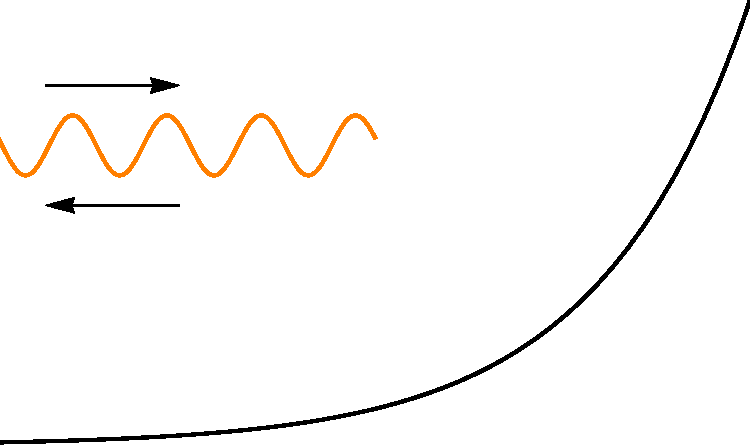
\includegraphics[width=.4\textwidth]{figures/Liouvillewall.pdf}
\caption{The vertex operator $V_P^{\rm in}$ (or $V_P^{\rm out}$, related by a phase) represents a scattering state in the presence of the Liouville wall.}\label{fig:liouvillewall}
\end{figure}

A far-reaching conjecture concerning the $c=1$ string theory is that it admits an exact dual description in terms of a double scaling limit of a gauged matrix quantum mechanics (MQM) \cite{Klebanov:1991qa}. %\footnote{The perturbative duality is reviewed by Klebanov, arXiv:hep-th/9108019. Further evidences and the extension of the duality are provided in Maldacena, JHEP \textbf{09} (2005), 078, Balthazar, Rodriguez, Yin, JHEP \textbf{04} (2019), 145; JHEP \textbf{01} (2019), 173; JHEP \textbf{05} (2023), 048, and Sen, JHEP \textbf{03} (2020), 005.} 
Essential features of the MQM are reviewed in Appendix \ref{app:mqm}. Various evidences and implications of the duality will be explored in sections \ref{conetree}, \ref{sec:zzfzzt} and \ref{sec:zzinst}.








\newpage

\section{Bosonic string interactions}
\label{chat:pertstring}

\subsection{Conformal gauge with moduli}
\label{stringscatt}

Heuristically, string scattering amplitudes should be captured by the path integral over worldsheet configurations that admit  punctures that represent asymptotic string states. Our earlier discussion of the conformal gauge has glossed over global issues that will become crucial in dealing with worldsheets with punctures and generally nontrivial topology. The worldsheet path integral with punctures, generalizing (\ref{zpath}), is formally
\ie\label{genusgnaive}
{1\over {\rm vol}({\cal G})} \int [Dg_{ab} DX^\mu] e^{-S_{\rm P}[g, X]} \prod_{i=1}^n \int d^2\sigma_i \sqrt{\det g(\sigma_i)}\, V_i(\sigma_i),
\fe
where the worldsheet surface $\Sigma$ is assumed to be compact, of a certain genus $h$ (``number of handles''), with $n$ ``vertex operators'' $V_1,\cdots,V_n$ inserted at the punctures $\sigma_i$. The $V_i$'s represent asymptotic string states, and are expected to transform as a scalar under worldsheet diffeomorphism, and of weight 2 with respect to Weyl transformation so that the functional integrand of (\ref{genusgnaive}) is diffeomorphism and Weyl invariant.

The surface $\Sigma$ can be covered with coordinate charts $U_i$, each of which is parameterized by the complex coordinate system $(z_i, \bar z_i)$ in which the metric $g_{ab}$ takes the Hermitian form
\ie\label{hermitform}
ds^2\equiv g_{ab}d\sigma^a d\sigma^b = 2 g_{z_i \bar z_i} dz_i d\bar z_i.
\fe
On the overlap between a pair of charts $U_i\cap U_j$, the coordinates $z_i$ and $z_j$ are related by a transition map 
\ie
z_i = f_{ij} (z_j, \bar z_j),~~~ \bar z_i = \bar f_{ij}(z_j, \bar z_j) .
\fe
The Hermiticity of the metric (\ref{hermitform}) simultaneously with respect to $z_i$ and $z_j$ implies that the transition map $f_{ij}$ must be holomorphic (and $\bar f_{ij}$ anti-holomorphic), such that
\ie
g_{z_j \bar z_j} = |\partial_{z_j} f_{ij}|^2 g_{z_i \bar z_i}.
\fe
Up to a Weyl transformation, the metric $g_{ab}$ is characterized entirely by the holomorphic coordinate system $z_i$ on the chart $U_i$, together with the set of compatible {\it holomorphic} transition maps $f_{ij}$. Moreover, two sets of holomorphic coordinate charts $(\{U_i\}; \{f_{ij}\})$ and $(\{U_i'\}; \{f_{ij}'\})$ that are related by holomorphic diffeomorphism give rise to Weyl equivalent metrics on $\Sigma$. Therefore, $\Sigma$ can be viewed as a 1-dimensional complex manifold, also known as a {\it Riemann surface}, whose complex structure is equivalent to the Weyl equivalence class of the metric $g_{ab}$.

The above construction can be generalized to a surface $\Sigma$ with $n$ punctures and metric $g_{ab}$. We can use the diffeomorphism and Weyl gauge transformations to set the locations of the punctures to $\sigma_1,\cdots, \sigma_n$, and the metric to
\ie\label{gffaa}
g_{ab} = \hat g_{ab}(t),
\fe
where $\hat g_{ab}(t)$ describes a family of fiducial metrics parameterized by the {\it moduli} $t\equiv (t^1, t^2, \cdots)$. More precisely, $t$ can be viewed as coordinates on the moduli space ${\cal M}_{h,n}$ of a Riemann surface with genus $h$ and $n$ punctures. It is explained in Appendix \ref{riemsurfsec} that the dimension of this moduli space is ${\rm dim}_{\mathbb{R}}({\cal M}_{h,n})=6h-6+2n$ (assuming $n\geq 3$ at $h=0$, and $n\geq 1$ at $h=1$).

The Faddeev-Popov procedure is applicable provided that we view (\ref{gffaa}) together with the choice of $\sigma_1,\cdots,\sigma_n$ as the gauge conditions, and treat the moduli $t^k$ on the same footing as the gauge parameters, except that after dividing by the volume of the gauge group in the end we will still have to integrate $t$ over the moduli space ${\cal M}_{h,n}$.
Under an infinitesimal diffeomorphism generated by a vector field $\delta v^a$ and Weyl transformation parameterized by a function $\delta\omega$, together with moduli variation $\delta t^k$, the gauge conditions vary by
\ie\label{gaugegnvar}
& \delta (g_{ab}-\hat g_{ab}(t)) = - \nabla_a \delta v_b - \nabla_b \delta v_a + 2\delta\omega g_{ab} - \sum_k \delta t^k {\partial \hat g_{ab}(t) \over \partial {t^k}},
\\
& \delta \sigma_i^a  = \delta v^a(\sigma_i).
\fe
The integration over $g_{ab}(\sigma)$ and $\sigma_i$ in (\ref{genusgnaive}) can be replaced with
\ie\label{fpprodc}
{1\over {\rm vol}({\cal G})} \int [Dg_{ab}] \prod_{i=1}^n d^2\sigma_i 
~\to~ 
\int_{{\cal M}_{h,n}} dt^k  \, \Delta_{\rm FP}[\hat g_{ab}, \sigma_i],
\fe
where the Faddeev-Popov determinant $\Delta_{\rm FP}$ is given by the Grassmann functional integral 
\ie\label{newfpdet}
&\Delta_{\rm FP}[\hat g_{ab}, \sigma_i] 
\\
&=  \int [Db_{ab} Dc^a] d\xi^k d\eta_i^a \, \exp\left\{ - S_{\rm gh}[\hat g, b, c] - {1\over 4\pi} \int d^2\sigma \sqrt{\det \hat g}\, b^{ab}  \sum_k\partial_{t^k} \hat g_{ab}(t) \xi^k - \sum_{i=1}^n \eta_i^a c^a(\sigma_i) \right\}.
\fe
The ``$c$-type'' ghosts $c^a(\sigma)$, $\xi^k$ are associated with the diffeomorphism vector field $\delta v^a$ and moduli variation $\delta t^k$, whereas the ``$b$-type'' ghosts $b^{ab}(\sigma)$ and $\eta_i^a$ are associated with the two gauge condition variations (\ref{gaugegnvar}). As in section \ref{firstattempt}, we have integrated out the $c$-type ghost associated with the Weyl transformation (denoted $\zeta$ in (\ref{fpdetearl})), which results in the constraint that $b^{ab}$ is traceless. $S_{\rm gh}$ is the same ghost action appearing in (\ref{fpdetearl}), but is supplemented in (\ref{newfpdet}) with the $\xi^k$-dependent term due to the moduli variation, and the $\eta_i^a$-dependent term due to the extra gauge conditions that fix the location of punctures. The finite-dimensional Grassmann integration over $\xi^k$ and $\eta_i^a$ in (\ref{newfpdet}) can be easily evaluated to give
\ie\label{fpbsonst}
\Delta_{\rm FP}[\hat g_{ab}, \sigma_i] = \int [Db_{ab} Dc^a] e^{-S_{\rm gh}[\hat g, b,c]} \prod_k {\cal B}_{t^k} \prod_{i,a} c^a(\sigma_i),
\fe
where
\ie\label{capbk}
{\cal B}_{t^k}\equiv {1\over 4\pi } \int d^2\sigma \sqrt{\det \hat g} \, b^{ab}\partial_{t^k}\hat g_{ab} .
\fe
At this point we have not specified the Polyakov action $S_P[g, X]$ apart from assuming its diffeomorphism and Weyl invariance. In particular, we may include in $S_P[g, X]$ a constant-dilaton term
\ie\label{topact}
{\phi_0\over 4\pi} \int d^2\sigma \sqrt{\det g} R(g) = \phi_0 \chi,
\fe
where $\chi=2-2h$ is the Euler characteristic of the worldsheet. Including (\ref{topact}) in the action would amount to multiplying (\ref{genusgnaive}) by the factor $e^{-\phi_0\chi} = (e^{\phi_0})^{2h-2}$. That is, for every additional ``handle'' or closed string loop, the amplitude (\ref{genusgnaive}) would acquire an extra factor $e^{2\phi_0}$. This means the string coupling constant, which will be defined more precisely in section \ref{sec:factortube}, is proportional to $e^{\phi_0}$.

As before, the functional integral over $X^\mu$ should define a $c=26$ matter CFT, that combines with the $bc$ ghost system to produce a worldsheet CFT that admits a nilpotent BRST symmetry. The gauge-fixed worldsheet path integral over the genus $h$ surface $\Sigma$ with $n$ punctures can be expressed as a CFT correlation function integrated with respect to the moduli $t^k$, namely
\ie\label{genusgstramp}
N_{h,n} \int_{{\cal M}_{h,n}} 
\left\langle \prod_k  dt^k {\cal B}_{t^k} \prod_{i=1}^n  \Big( \prod_{a=1,2} c^a(\sigma_i) \Big)  \sqrt{\det\hat g(\sigma_i)} V_i(\sigma_i) \right\rangle_{\Sigma, \hat g(t)}
\equiv {\cal A}_h[V_1,\cdots, V_n] ,
\fe
where $N_{h,n}$ is a normalization constant that will be specified later.
The vertex operator $V_i(\sigma_i)$, defined with appropriate regularization in the path integral formalism, is now viewed as a quantum local operator in the matter CFT that is a Virasoro primary of weight $(1,1)$. In particular, its combination with the ghost fields $c^1(\sigma_i) c^2(\sigma_i)$ is a BRST-closed operator of the OCQ form, and represents a physical string state. The correlation function in (\ref{genusgstramp}) produces a top degree differential form on the moduli space ${\cal M}_{g,n}$. Note that the moduli dependence comes from the metric $\hat g_{ab}(t)$ on the worldsheet surface $\Sigma$ as well as the puncture locations $\sigma_i$ (which a priori depend on $t$). The precise interpretation of ${\cal A}_h[V_1,\cdots, V_n]$ as the genus $h$, $n$-point connected S-matrix element will be clarified in section \ref{bosstringunitary}.


\subsection{Reformulation in terms of holomorphic data}
\label{sec:bosholdata}

While the amplitude (\ref{genusgstramp}) involves the fiducial metric $\hat g(t)$, the Weyl invariance of the worldsheet CFT is such that the correlator in question should only depend on the Weyl-equivalence class of $\hat g(t)$, which is entirely characterized by the complex structure of an underlying Riemann surface (with respect to which the metric $\hat g(t)$ is Hermitian). Furthermore, the integration over the locations of $b$ ghost insertions in (\ref{genusgstramp}) is not obviously well-defined, due to the singular OPE between $b$ and $c$. Both of these issues will be resolved by reformulating (\ref{genusgstramp}) in a way that only makes reference to the holomorphic data of a Riemann surface.

Let us begin with the defining data of a Riemann surface $\Sigma(t)$, namely a collection of holomorphic coordinate charts $U_i$ together with the holomorphic transition maps on their overlaps $U_i\cap U_j$, of the form
\ie
z_i = f_{ij}(z_j; t).
\fe
In particular, the moduli dependence is completely characterized by the dependence of the transition functions $f_{ij}$ on the real parameters $t^k$.\footnote{The moduli space ${\cal M}$ of a Riemann surface also admits a natural complex structure, and we could alternatively work with complex moduli parameters that are holomorphic coordinates on ${\cal M}$, but this is not needed at the moment.} An infinitesimal moduli deformation $t^k \mapsto t'^k = t^k+\delta t^k$ produces a Riemann surface $\Sigma(t')$, whose local holomorphic coordinates $z_i'$ are related by transition maps
\ie\label{zprimetrans}
z_i' = f_{ij}(z_j'; t')
\fe
on $U_i\cap U_j$. One can find an infinitesimal {\it non-holomorphic} diffeomorphism relating $z_i$ to $z_i'$, of the form
\ie\label{zzpmap}
z'_i = z_i +  \sum_k\delta t^k v_{k, i}^{z_i}(z_i, \bar z_i),
\fe
where $v_{k,i}\equiv v_{k,i}^{z_i} \partial_{z_i}$ is a vector field defined on the patch $U_i$. Plugging (\ref{zzpmap}) into (\ref{zprimetrans}) and keep only first order terms in $\delta t^k$ yields the relation
\ie\label{vvdiff}
v_{k,i}^{z_i} &= v_{k,j}^{z_j} \partial_z f_{ij}(z_j; t) + \partial_{t^k} f_{ij}(z_j; t)
\\
&= v_{k,j}^{z_i} + \left.{\partial z_i\over \partial t^k}\right|_{z_j},
\fe
where in the second line $v_{k,j}^{z_i}$ stands for the holomorphic component of the vector field $v_{k,j}$ in the $z_i$ coordinate system, namely $v_{k,j} \equiv v_{k,j}^{z_j} \partial_{z_j} = v_{k,j}^{z_i} \partial_{z_i}$. 

We would like to compare a Hermitian metric on $\Sigma(t)$ with one on $\Sigma(t')$ up to Weyl transformation. Restricting to the patch $U_i$, it suffices to compare the metric $ds^2 = dz_i d\bar z_i$ with $ds^2=dz_i' d\bar z_i'$. The latter can be expressed in the $(z_i, \bar z_i)$ coordinate system as
\ie
ds^2 &= \left| dz_i (1+  \sum_k\delta t^k \partial_{z_i} v_{k,i}^{z_i} ) + d\bar z_i  \sum_k\delta t^k \bar\partial_{\bar z_i} v_{k,i}^{z_i} \right|^2
\\
&= e^{2\delta\omega} \left[ dz_i d\bar z_i + \sum_k \delta t^k \left( \partial_{z_i} \overline{v_{k,i}^{z_i}} dz_i^2 + \bar\partial_{\bar z_i} v_{k,i}^{z_i} d\bar z_i^2\right) \right],
\fe
from which we read off the metric variation
\ie\label{delgexplc}
\delta g_{z_i \bar z_i} = \delta\omega, ~~~ \delta g_{z_i z_i} =  \sum_k\delta t^k\partial_{z_i} \overline{v_{k,i}^{z_i}},~~~ \delta g_{\bar z_i\bar z_i} =  \sum_k\delta t^k \bar\partial_{\bar z_i} v_{k,i}^{z_i}.
\fe
The variation $\delta g_{z_i\bar z_i}$ can be undone by a Weyl transformation and is inconsequential, whereas $\delta g_{z_i z_i}$ and $\delta g_{\bar z_i\bar z_i}$ correspond to the traceless part of $\partial_{t^k} g_{ab}$ that appear in (\ref{genusgstramp}). In terms of the Weyl invariant Beltrami differential
\ie\label{beltramidif}
(\mu_k)_a{}^b = {1\over 2}\hat g^{bc} \partial_{t^k} \hat g_{ac},
\fe
we can express the last two equations of (\ref{delgexplc}) as 
\ie
(\mu_k)_{\bar z_i}{}^{z_i} =\bar\partial_{\bar z_i} v_{k,i}^{z_i} ,~~~ (\mu_k)_{z_i}{}^{\bar z_i} =  \partial_{z_i} \overline{v_{k,i}^{z_i}} .
\fe
The $b$ ghost insertion appearing in (\ref{genusgstramp}), namely (\ref{capbk}), can be rewritten as
\ie
{\cal B}_{t^k} &= {1\over 2\pi} \int d^2z \big[ b_{zz} (\mu_k)_{\bar z}{}^z + b_{\bar z\bar z} (\mu_k)_z{}^{\bar z} \big]
\\
&= \sum_j {1\over 2\pi} \int_{D_j} d^2z_j \big( b_{z_j z_j}  \bar\partial_{\bar z_j} v_{k,j}^{z_j} + b_{\bar z_j \bar z_j} \partial_{z_j}\overline{v_{k,j}^{z_j}} \big) .
\fe
Note that the second line is a more precise expression for the integration in the first line, where the Riemann surface $\Sigma$ is divided into the domains $D_j\subset U_j$, on which the integration is appropriately performed in the local coordinate system $(z_j, \bar z_j)$. We now use the holomorphy of $b_{zz}$, i.e. the operator equation $\bar\partial_{\bar z} b_{zz}=0$, to turn the integration over the domain $D_j$ into a contour integral over the boundary $\partial D_j\equiv C_j$, yielding\footnote{This derivation is not affected by the presence of $c$ ghost insertions at the punctures, as the vector field $v_{k,i}$ appearing in (\ref{zzpmap}) can be set to zero on a patch $U_i$ that contains the puncture.}
\ie\label{bktempaex}
{\cal B}_{t^k} & =  \sum_j \oint_{C_j}  \left( {dz_j\over 2\pi i} b_{z_j z_j}  v_{k,j}^{z_j} - {d\bar z_j\over 2\pi i} b_{\bar z_j \bar z_j} \overline{v_{k,j}^{z_j}} \right).
\fe
Each contour $C_i$ can be further divided as $C_i = \sum_{j\not=i} C_{ij}$, where $C_{ij}$ is the segment on which $C_i$ and $C_j$ overlap, and the orientation of $C_{ij}$ is defined to agree with that of $C_i$ (and opposite of $C_j$). In particular, our convention is such that $C_{ji}=-C_{ij}$. Splitting each contour integral in (\ref{bktempaex}) in this manner and using the relation (\ref{vvdiff}), we arrive at an expression for ${\cal B}_{t^k}$ that makes reference only to the holomorphic transition maps between charts,
\ie\label{bkfactor}
{\cal B}_{t^k} =  \sum_{(j\ell)} \int_{C_{j\ell}}  \left( {dz_j\over 2\pi i} b_{z_j z_j}  \left.{\partial z_j\over \partial t^k}\right|_{z_\ell} - {d\bar z_j\over 2\pi i} b_{\bar z_j \bar z_j} \left.{\partial \bar z_j\over \partial t^k}\right|_{\bar z_\ell}  \right),
\fe
where the summation is taken over every unordered pair $(j\ell)$ once (note that the summand is in fact symmetric with respect to exchanging $j,\ell$). As a special case, if the domains $D_j$ are chosen to be the components of a pair-of-pants decomposition of $\Sigma$, then for each $j$ there is a unique $\ell$ such that $C_{j\ell}$ is non-empty, and is given by $\partial D_j=-\partial D_\ell$.

\begin{figure}[h!]
\centering
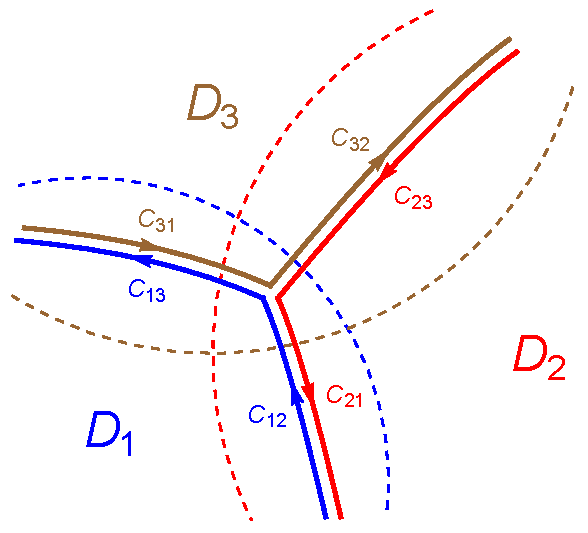
\includegraphics[width=.4\textwidth]{figures/overlappingdomains.pdf}
\caption{The overlapping charts $U_1, U_2, U_3$, bounded by the dashed lines in blue, red, and brown respectively, contain the domains $D_1$, $D_2$, $D_3$ separated by the contours $C_{12}=-C_{21}$, $C_{23}=-C_{32}$, and $C_{13}=-C_{31}$.}\label{fig:overlappingdomains}
\end{figure}

The above construction is straightforwardly generalized to a Riemann surface with punctures, where each puncture is contained in a chart $W_i$ that may be taken to be a disc. Without loss of generality, we may take the local holomorphic coordinate $w_i$ on $W_i$ to be such that the puncture, where we insert the vertex operator $V_i$, is located at $w_i=0$. Now suppose there is another chart $U_i$ that overlaps with $W_i$ along an annulus region but does not contain the puncture at the origin of $W_i$, whose coordinate $z_i$ is related to $w_i$ by a simple linear shift
\ie
w_i =  z_i - u_i.
\fe
An infinitesimal shift of the location of the puncture on the Riemann surface can be equivalently characterized as an infinitesimal shift of the parameter $u_i$, without changing any of the other transition maps. In this sense, we can view $u_i$ as a complex modulus, or a pair of the real moduli parameter $t^k$'s. The vertex operator $V_i$ together with the moduli associated with its location produces an operator insertion in (\ref{genusgstramp})
\ie\label{ubbvex}
{\cal B}_{\bar u_i} {\cal B}_{u_i} (c\widetilde c V_i)^{(w_i)}(0),
\fe
where the superscript $(w_i)$ indicates that the vertex operator is of the said form in $w_i$-coordinate, and ${\cal B}_{u_i}$ is according to (\ref{bkfactor})
\ie\label{bminusones}
{\cal B}_{u_i} = \oint_{C_i} {dw_i\over 2\pi i} b_{w_iw_i} \left. {\partial w_i \over \partial u_i}\right|_{z_i} = - b_{-1},
\fe
where the contour $C_i$ encloses the puncture at $w_i=0$, and $b_{-1}$ is understood as acting on the vertex operator at $w_i=0$. Likewise, ${\cal B}_{\bar u_i}$ is equivalent to $-\widetilde b_{-1}$. Therefore, (\ref{ubbvex}) can be equivalently written as
\ie\label{intverta}
(\widetilde b_{-1} b_{-1}\cdot c\widetilde c V_i)^{(w_i)}(0) = V_i^{(w_i)}(0) = V_i^{(z_i)}(u_i).
\fe
That is, if we identify the location of a puncture with a complex modulus, then the corresponding $b$ ghost insertions effectively strip off the $c$ ghosts at the puncture, leaving only the matter CFT primary $V_i$ to be integrated.

Finally, we can recast (\ref{genusgstramp}) in the concise form
\ie\label{omegaone}
{\cal A}_h[V_1, \cdots, V_n] = N_{h,n} \int_{{\cal M}_{h,n}} \Omega_{6h-6+2n},
\fe
where $\Omega_p$ is the degree $p$ component of the differential form
\ie\label{omegatwo}
& \Omega = \bigg\langle e^{\cal B} \prod_{i=1}^n {\cal V}_i \bigg\rangle_{\Sigma}
\fe
on the moduli space ${\cal M}_{h,n}$. Here ${\cal V}_i$ is a BRST-closed operator, e.g. the OCQ representative $c\tilde c V_i$, and ${\cal B}$ is the 1-form
\ie\label{calboneform}
{\cal B} \equiv \sum_k dt^k {\cal B}_{t^k} .
\fe
The multiplication of differential forms is defined by wedge product, under which $dt^k$ is Grassmann-odd. Since the $b$ ghost or ${\cal B}_{t^k}$ (\ref{bktempaex}) is Grassmann-odd, ${\cal B}$ is Grassmann-even and hence the exponentiation of ${\cal B}$ in (\ref{omegatwo}) makes sense.\footnote{Whether a 1-form such as $dt^k$ should be treated as commuting or anti-commuting with a Grassmann-odd field such as $b$ is a matter of convention that affects the normalization constant $N_{h,n}$. We will adopt the latter convention and treat the differential forms on the same footing as a Grassmann-odd field.}


\subsection{The ghost number anomaly}
\label{sec:bcghost}

Recall from (\ref{jbctope}) that the holomorphic $bc$ ghost number current $j_{\rm gh}$ (\ref{bcghostcurr}) is not a Virasoro primary. On a curved worldsheet, an analysis of the contact term in the operator product of the trace of the stress-energy tensor with $j_{\rm gh}$, analogous to that of section \ref{weylanomalsec}, shows that the ghost number symmetry is anomalous due to 
\ie\label{jbcanom}
\nabla_a j_{\rm gh}^a = -{3\over 4} R(g),
\fe
where $R(g)$ is the Ricci scalar associated to the worldsheet metric $g_{ab}$. Integrating (\ref{jbcanom}) over the worldsheet, one finds that a correlation function $\langle {\cal O}\rangle_\Sigma$ of the $bc$ CFT on a genus $h$ surface $\Sigma$ can be non-vanishing only if ${\cal O}$ carries holomorphic ghost number $3-3h$. There is an analogous anomaly of the anti-holomorphic $\widetilde b\widetilde c$ ghost number. 

Indeed, the correlator appearing in (\ref{genusgstramp}) involves a total of $\dim({\cal M}_{h,n})$ insertions of $b$ and $\wt b$, and a total of $2n$ insertions of $c$ and $\wt c$. Their difference $\dim({\cal M}_{h,n}) - 2n = 6h-6$ is precisely as required by the ghost number anomaly.

In particular, the simplest non-vanishing correlation function on the Riemann sphere involves the insertion of 3 $c$'s and 3 $\wt c$'s. The result is fixed by conformal symmetry up to a normalization constant. We will adopt the normalization convention of $bc$ path integral such that
\ie\label{ccoresign}
\left\langle \prod_{i=1}^3 c(z_i)\widetilde c(\bar z_i) \right\rangle = |z_{12} z_{13} z_{23}|^2.
\fe
In terms of the state $|\downarrow,\downarrow\rangle$ that corresponds to the operator $c\wt c(0)$, (\ref{ccoresign}) is equivalent to the inner product
\ie\label{ccoresigna}
\langle\langle \downarrow, \downarrow| c_0 \widetilde c_0 |\downarrow, \downarrow\rangle %= \langle\langle \downarrow, \downarrow|\uparrow, \uparrow\rangle 
= 1,
\fe
where $\langle\langle\,\cdot\,|$ stands for the {\it BPZ conjugate}, defined by
\ie\label{bpzconjdef}
\langle \langle \psi|\phi\rangle \equiv \left\langle [\psi(0)]^I \phi(0)\right\rangle
\fe
for any pair of states $\phi, \psi$. Here $[\psi(0)]^I$ stands for the conformal transformation of $\psi(0)$ with respect to the inversion map $z'=1/z$. Note that when it comes to the ghost system, we will always work with inner products defined through the BPZ conjugate, rather than introducing any notion of Hermitian conjugation.



%Since the $bc$ CFT is free, we can explicitly evaluate its correlation functions through a Gaussian functional integral. Let us define the differential operator ${\cal P}$ that takes a vector field on $\Sigma$ to a symmetric traceless tensor,
%\ie
%({\cal P} c)_{ab} \equiv {1\over 2} \left(\nabla_a c_b + \nabla_b c_a - g_{ab} \nabla_d c^d\right).
%\fe
%With respect to the pairing of tensor fields defined by 
%\ie\label{ffppair}
%(f, f') \equiv \int d^2\sigma \sqrt{g}\, f^{ab} f'_{ab},
%\fe
%the transpose of ${\cal P}$ acts on a symmetric traceless tensor according to
%\ie
%({\cal P}^T b)^a = - \nabla^b b_{ab}.
%\fe
%The $bc$ ghost action can be written as
%\ie
%S_{\rm gh} = {1\over 2\pi} (b, {\cal P} c) = {1\over 2\pi} ({\cal P}^T b, c).
%\fe
%${\cal P}^T$ is also the same as the adjoint of ${\cal P}$ with respect to a Hermitian inner product defined analogously to (\ref{ffppair}) but with complex conjugation on one of the tensor fields. In particular, ${\cal P}^T{\cal P}$ and ${\cal P}{\cal P}^T$ are positive semidefinite Hermitian operators. We can find an orthonormal basis $v_n$ for vector fields on $\Sigma$ that diagonalizes ${\cal P}^T{\cal P}$,
%\ie{}
%& {\cal P}^T{\cal P} v_n = \lambda_n v_n,
%\fe
%where the eigenvalues $\lambda_n$ are non-negative. The zero eigen-vector-fields will be denoted $v_j^{(0)}$. If $\lambda_n$ is nonzero, we can define
%\ie
%u_n = (\lambda_n)^{-{1\over 2}} {\cal P} v_n.
%\fe
%$u_n$ are a set of orthonormal symmetric traceless tensor fields that obey
%\ie{}
%& {\cal P}{\cal P}^T u_n = \lambda_n u_n, ~~~ v_n =  (\lambda_n)^{-{1\over 2}}{\cal P}^T u_n.
%\fe
%We can complete $u_n$ into a basis of symmetric traceless tensor fields including also the zero modes $u_k^{(0)}$. Note that while the nonzero eigenvectors of ${\cal P}^T{\cal P}$ and ${\cal P}{\cal P}^T$ come in pairs, the zero eigenvectors do not. Expanding
%\ie\label{bcexpfou}
%b_{ab}(\sigma) = \sum_n b_n (u_n)_{ab}(\sigma),~~~ c^a(\sigma) = \sum_n c_n (v_n)^a(\sigma),
%\fe
%we can write the functional integral of the $bc$ system as
%\ie\label{bcghosintexpl}
%\int [Db Dc] e^{-S_{\rm gh}}\cdots = \int \prod_n db_n \prod_m dc_m \, \exp\left(-{1\over 2\pi} \sum_n \sqrt{\lambda_n} b_n c_n \right) \cdots
%\fe
%where $\cdots$ represents general operator insertions. The zero modes of $b_{ab}$ and $c^a$, i.e. the coefficients of $u_k^{(0)}$ and $v_j^{(0)}$ in the expansion (\ref{bcexpfou}), do not appear in the ghost action $S_{\rm gh}$. Thus, the functional integral (\ref{bcghosintexpl}) vanishes unless the operator insertion $\cdots$ includes precisely the zero modes of $b_{ab}$ and $c^a$.
%
%The condition ${\cal P}v_j^{(0)}=0$ is also known as the conformal Killing equation, and $v_j^{(0))}$ is a basis of conformal Killing vector fields. $u_k^{(0)}$, on the other hand, represent metric deformations $\delta g_{ab}$ that are orthogonal to all diffeomorphism and Weyl variations (\ref{diffweag}). In other words, zero modes of $c^a$ are in 1-1 correspondence with the conformal Killing vector fields, whereas the zero modes of $b_{ab}$ are in 1-1 correspondence with deformations of the moduli, $\delta t^k$. Now we see in that the $b$ and $c$ insertions in the correlation function appearing on the RHS of (\ref{genusgstramp}) precisely match the number of zero modes. It is conventional to define the Beltrami differential
%\ie
%(\mu_k)_{ab} \equiv {1\over 2} \partial_{t^k} \hat g_{ab}(t),
%\fe
%so that we can write
%\ie
%{1\over 4\pi } \int d^2\sigma \sqrt{\hat g} \, b^{ab}\partial_{t^k}\hat g_{ab} \equiv {1\over 2\pi} (b, \mu_k).
%\fe
%The $bc$ CFT correlator appearing in (\ref{genusgstramp}) can be evaluated as
%\ie\label{bcdet}
%\left\langle \prod_k {1\over 2\pi}(b, \mu_k) \prod_{i,a} c^a(\hat\sigma_i) \right\rangle_{\Sigma} = \left[\det{}'{{\cal P}^T{\cal P}\over 2\pi}\right]^{1\over 2} \det {(u_k^{(0)}, \mu_\ell)\over 2\pi} \det_{j, (i,a)} v_j^a(\hat\sigma_i),
%\fe
%where $\det'$ is the functional determinant taken over nonzero modes of ${\cal P}$.




\subsection{Boundaries of the moduli space}
\label{sec:boundarymoduli}

As a physical observable, it is essential that the amplitude (\ref{omegaone}) is BRST invariant in the sense that it is independent of the choice of the BRST representative ${\cal V}_i$ in a given cohomology class. This may not be immediately evident, as the $b$ ghost insertions in (\ref{omegatwo}) are not BRST-closed. Using the non-holomorphic representation (\ref{capbk}), we can write the BRST transformation of ${\cal B}_{t^k}$ as
\ie\label{qbbk}
Q_B \cdot {\cal B}_{t^k} = {1\over 4\pi} \int d^2\sigma \sqrt{\det\hat g}\, T^{ab} \partial_{t^k} \hat g_{ab}. 
\fe
Inserting (\ref{qbbk}) into a correlator on $\Sigma$ gives
\ie\label{qbonbmuk}
\left\langle Q_B \cdot {\cal B}_{t^k} \, {\cal O} \right\rangle_{\Sigma, \hat g(t)} &= {1\over 4\pi}\int d^2\sigma \sqrt{\det\hat g}\,  \partial_{t^k} \hat g_{ab} \left\langle T^{ab}(\sigma)\,  {\cal O} \right\rangle_{\Sigma, \hat g(t)} = - \partial_{t^k} \left\langle {\cal O} \right\rangle_{\Sigma, \hat g(t)} .
\fe
For instance, if we shift ${\cal V}_1$ in (\ref{omegatwo}) by a $Q_B$-exact operator of the form $\delta {\cal V}_1 = Q_B\chi_1$, the differential form $\Omega_p$ shifts by
\ie\label{omegapbrstvar}
\delta\Omega_p &= \bigg\langle {1\over p!}{\cal B}^p (Q_B\chi_1) \prod_{i=2}^n {\cal V}_i \bigg\rangle_{\Sigma}
=- \bigg\langle (Q_B {\cal B}) {1\over (p-1)!}{\cal B}^{p-1} \chi_1 \prod_{i=2}^n {\cal V}_i \bigg\rangle_{\Sigma}
\\
&= - \sum_k dt^k \partial_{t^k} \bigg\langle {1\over (p-1)!}{\cal B}^{p-1} \chi_1 \prod_{i=2}^n {\cal V}_i \bigg\rangle_{\Sigma}.
\fe
The corresponding variation of the amplitude (\ref{omegaone}) is the integral of a total derivative over the moduli space ${\cal M}_{h,n}$, which vanishes up to possible boundary terms.
%\ie
%\Omega_p[Q_B (\otimes_i {\cal V}_i)] &\equiv \Omega_p[ Q_B {\cal V}_1,{\cal V}_2,\cdots, {\cal V}_n] +  \Omega_p[  {\cal V}_1,Q_B{\cal V}_2,\cdots, {\cal V}_n] + \cdots + \Omega_p[ {\cal V}_1,{\cal V}_2,\cdots, Q_B {\cal V}_n] \\ & = -d\Omega_{p-1}[{\cal V}_1,\cdots, {\cal V}_n].
%\fe 

The boundary of the moduli space $\partial {\cal M}_{h,n}$ is the union of components: {\bf (1)} The loci in ${\cal M}_{h,n}$ where the Riemann surface $\Sigma$ pinches into a pair of surfaces $\Sigma_1$ and $\Sigma_2$ joined at a pair of punctures. The genus $g_i$ and number of punctures $n_i$ of $\Sigma_i$, $i=1,2$, obey $g_1+g_2=h$, $n_1+n_2=n+2$.  {\bf (2)} The loci in ${\cal M}_{h,n}$ where a handle of $\Sigma$ pinches off, so that $\Sigma$ degenerates into a surface $\Sigma'$ of genus $h-1$ and $n+2$ punctures, with a pair of punctures joined together. %\fixme{show figures} 

Let us first inspect a special case of  {\bf (1)}, $g_1=0$ and $n_1=3$, which is equivalent to the limit where a pair of punctures collide and $\Sigma$ reduces to $\Sigma_2$ (of genus $g_2=h$ and $n_2=n-1$ punctures). In the vicinity of this boundary component of the moduli space, the vertex operators ${\cal V}_1$ and ${\cal V}_2$ are close to one another. Up to a Weyl transformation, we may assume that the fiducial metric $\hat g_{ab}$ takes the Euclidean form $\delta_{ab}$ in a coordinate system that covers the location of both ${\cal V}_1$ and ${\cal V}_2$. By the argument around (\ref{bminusones}), the $b$ ghost insertions around ${\cal V}_i$ converts the latter into the weight $(1,1)$ matter CFT primary $V_i(z_i, \bar z_i)$, whose coordinates $(z_i,\bar z_i)$ are moduli to be integrated. We can replace the product of $V_1$ and $V_2$ with their OPE, organized in the form
\ie\label{vvoope}
V_1(z_1, \bar z_1) V_2(z_2, \bar z_2) = \sum_n z_{12}^{h_n-2} \bar z_{12}^{\widetilde h_n - 2} {\cal O}_n(z_2, \bar z_2)
\fe
where ${\cal O}_n$ are matter CFT operators of weight $(h_n, \widetilde h_n)$. If there are terms on the RHS of (\ref{vvoope}) with $h_n=\widetilde h_n\leq 1$, the moduli integral of (\ref{omegaone}) in particular includes an integration over $z_1$ that potentially diverges near the boundary locus $z_1=z_2$.
%A priori, if there are operators ${\cal O}_n$ appearing on the RHS of (\ref{vvoope}) with $h_n=\widetilde h_n\leq 1$, the integral over $z_1$ diverges near $z_1=z_2$. If we cut off the $z_1$ integral by excluding a small disc of radius $\epsilon$ centered at $z_2$, we encounter a power divergence of order $\epsilon^{2(h_n-1)}$ for $h_n=\widetilde h_n<1$, and a logarithmic divergence of order $\log(1/\epsilon)$ if $h_n=\widetilde h_n=1$. The power divergence can be canceled by a local counter term and is unphysical, whereas the log divergence has the following physical interpretation.
To understand the nature of this divergence, suppose each $V_i$ represents a string state of spacetime momentum $k_i^\mu$, that obeys the mass-shell condition (\ref{masshe}) $-k_i^2 = m_i^2 = {4\over \A'}(N_i-1)$ for a non-negative integer oscillator level $N_i$. The OPE of the free boson CFT is such that ${\cal O}_n$ carries spacetime momentum charge $k_1^\mu+k_2^\mu$ and has conformal weight $(h_n,\widetilde h_n)$ necessarily of the form
\ie
h_n={\A'\over 4} (k_1+k_2)^2+\ell_n, ~~~~ \widetilde h_n={\A'\over 4} (k_1+k_2)^2+\widetilde \ell_n,
\fe
for some non-negative integer oscillator levels $\ell_n, \widetilde \ell_n$. One expects that the moduli integration of (\ref{omegaone}) generically suffers a power divergence near $z_1=z_2$ for sufficiently large timelike $(k_1+k_2)^\mu$, and must be defined with a suitable regularization in order to produce a sensible string scattering amplitude.

%As is familiar in perturbative quantum field theory and partially established on general grounds of causality, 
A general expectation on scattering amplitudes in a causal relativistic quantum theory is that the connected S-matrix elements (to be defined more precisely in section \ref{bosstringunitary}) should admit suitable analytic continuation with respect to the momenta $k_i^\mu$, subject to the constraints of mass-shell condition and momentum conservation, and up to singularities that typically can be interpreted as due to the propagation of intermediate on-shell particles. In particular, it suggests the following regularization of the aforementioned power divergence: we begin with momenta $k_1^\mu$ and $k_2^\mu$ that are on-shell and obey momentum conservation, in a complex domain where ${\rm Re} \left[(k_1+k_2)^2 \right]$ is sufficiently large and positive so that the integral of (\ref{vvoope}) converges near $z_1=z_2$, and analytically continue the resulting amplitude to generic values of $k_1, k_2$. In the end, this is equivalent to simply dropping power divergences in the moduli integration.\footnote{As a toy example, consider the integral
\ie
\int_{|z|<1} d^2z |z|^{x-2} = {2\pi \over x},~~~ {\rm Re}(x)>0.
\fe
Its analytic continuation to ${\rm Re}(x)<0$ is
\ie
{2\pi\over x} = \lim_{\epsilon\to 0} \left[ \int_{\epsilon<|z|<1} d^2z |z|^{x-2} - {2\pi\over x} \epsilon^x \right],
\fe
which is equivalent to dropping the power divergence.} Furthermore, there is no boundary term in the integral of (\ref{omegapbrstvar}) near $z_1=z_2$ that would spoil the BRST invariance of the amplitude.

A logarithmic divergence may occur when $h_n=\widetilde h_n=1$, near which the (regularized) integral in $z_1$ near $z_1=z_2$ produces a pole factor
\ie
{1\over (k_1+k_2)^2 + M^2},
\fe
where $M^2={4\over \A'}(N-1)$ for some non-negative integer $N$. We will see in section \ref{sec:factortube} that the residues at these poles are precisely accounted for by intermediate on-shell 1-particle states, as required by the unitarity of the S-matrix. 
%A similar argument applies to the situation where $\Sigma_{g,n}$ pinches into $\Sigma_{g_1, n_1}$ and $\Sigma_{g_2, n_2}$. Up to a conformal transformation, the pinching limit amounts to having a long cylinder of circumference $2\pi$ and length $2\pi t$ connecting $\Sigma_{g_1, n_1}$ and $\Sigma_{g_2, n_2}$, with $t\to \infty$. States propagating through the cylinder has spacetime momentum $P^\mu = \sum_{i=1}^{n_1-1} k_i^\mu = -\sum_{i=n_1}^{n} k_i^\mu$, where $k_1, \cdots, k_{n_1-1}$ are the momenta of vertex operators on $\Sigma_{g_1, n_1}$, and $k_{n_1},\cdots, k_{n}$ are the momenta of vertex operators on $\Sigma_{g_2, n_2}$. The correlation function of the vertex operators is suppressed by the propagator along the cylinder,
%\ie\label{tllfac}
%\exp\left[ - 2\pi t (L_0 + \widetilde L_0) \right] = \exp\left[ - 2\pi t\left( {\A'\over 2}P^2 + N + \widetilde N - 2 \right) \right],
%\fe
%where $N$ and $\widetilde N$ are the holomorphic and anti-holomorphic oscillator levels. Provided that $n_1, n_2\geq 3$, we can always define the amplitude by analytic continuation from a domain in which ${\rm Re}(P^2)$ is sufficiently large and positive, where the moduli integral over the large $t$ region converges. When the momenta are arranged such that $P^2$ approaches $-M^2$ for some mass value $M$ of a string state, the analytic continuation results in a pole of the form $(P^2+M^2)^{-1}$, as will be analyzed in more detail in section \ref{bosstringunitary}.
A similar analysis is applicable to any boundary component of the moduli space where $\Sigma$ pinches into a pair of surfaces $\Sigma_1$, $\Sigma_2$, provided that each $\Sigma_i$ has at least 3 punctures.

There are two exceptional types of boundaries of the moduli space that must be considered separately:  {\bf (1a)} $\Sigma_1$ has genus $h_1\geq 1$ with $n_1=2$ punctures, and  {\bf (1b)} $\Sigma_1$ has genus $h_1\geq 1$ with $n_1=1$ puncture. A potentially divergent moduli integral from {\bf (1a)} indicates a mass and field renormalization of the string state at the punctures, whereas a potentially divergent moduli integral from {\bf (1b)} would indicate that the spacetime background is not a true vacuum configuration. A fully consistent treatment of the mass and field renormalization as well as shifting the vacuum background field requires an off-shell extension of the string amplitude, and will be discussed in the string field theory framework in Chapter \ref{sftchap}.

 
%In the case  {\bf (1a)}, the momentum $P^\mu = k_1^\mu$ flowing through the cylinder is always on-shell, and potentially leads to a divergence in the $t$-integral. Such a divergence, if present, should be canceled by a mass renormalization of the string state in question. This will be addressed in section \ref{offshellamp}. In the case (b), the momentum $P^\mu$ is always zero; a potential divergence that results from the $t$-integral amounts to a tadpole diagram that ought to be canceled by a shift of the background string fields in spacetime.

As for {\bf (2)} the boundary locus of ${\cal M}_{h,n}$ where a handle of $\Sigma$ pinches off, we will see in section \ref{sec:oneloop} that a divergence arises due to the propagation of the closed string tachyon. While this spells doom for the quantum critical bosonic string theory at least at the level of perturbation theory, the problem is evaded in the tachyon-free bosonic $c=1$ string theory introduced in section \ref{conesec}.

%One may further worry about the higher codimension locus in ${\cal M}_{g,n}$ where different boundary components meet. An example of this is when $\Sigma_{g,n}$ degenerates into a torus joined to a genus $g-1$ surface, and simultaneously pinching off the handle of the torus. This amounts to the insertion of a local vertex operator, whose coefficient may be logarithmically divergent due to the moduli integral. The interpretation of such a log divergence is a string-loop contribution to the Weyl anomaly on the worldsheet, which should be canceled by an adjustment of the spacetime background field due to the string-loop corrections to the spacetime equation of motion.



\subsection{The string S-matrix}
\label{bosstringunitary}

Quantum scattering theory is formulated based on the idea that under time evolution, every quantum state evolves into a superposition of asymptotic states that describe far-separated wave packets of particles, whose interactions diminish with distance. In (closed) string perturbation theory, it is assumed that all asymptotic particles are closed strings, and that the full (multi-string) Hilbert space is spanned by the basis of in-states
\ie\label{instates}
|\{V_i(k_i)_{1\leq i\leq m} \}\rangle^{in},
\fe
where each $V_i(k_i)$ stands for a vertex operator that represents a single string state with spacetime momentum $k_i^\mu$. The in-state (\ref{instates}) is a scattering state that consists of $m$ closed strings in the far past. More precisely, (\ref{instates}) is defined as a limiting quantum state which, in the far past, asymptotes to $m$ far-separated wave packets of individual closed string labeled by the vertex operator $V_i$, whose spacetime momentum is concentrated around $k_i^\mu$ with positive energy $k_i^0>0$. 

Likewise, the same multi-string Hilbert space is spanned by the basis of out-states
\ie\label{outstates}
|\{V_i(k_i)_{1\leq i\leq m} \}\rangle^{out}
\fe
labeled by the same set of vertex operators $V_i(k_i)$ as in (\ref{instates}), but now characterize the closed strings in the far future. The string S-matrix is defined as the unitary operator that relates the in- and out- bases,
\ie
{\cal S}|\{V_i (k_i)_{1\leq i\leq m} \}\rangle^{out} = 
|\{V_i(k_i)_{1\leq i\leq m} \}\rangle^{in}.
\fe
Equivalently, we can work with the matrix elements ${}^{out}\langle \B |{\cal S}|  \A \rangle^{out} = {}^{out}\langle\B | \A \rangle^{in}$, and will subsequently omit the superscript {\it out} in denoting the S-matrix element as simply $\langle \B |{\cal S}|  \A\rangle$. A basic consequence of locality of interaction is that the S-matrix obeys the cluster property
\ie\label{conncluster}
\langle \B| {\cal S} |\A\rangle = \sum_{\{\A_I, \B_I\}} \prod_I \langle \B_I| {\cal S}^{\rm conn} |\A_I\rangle,
\fe
where the sum is taken over all unordered simultaneous partitions $\{\A_I, \B_I\}$ of the sets $\A,\B$ labeling the asymptotic particles. The connected S-matrix element $\langle\B|{\cal S}^{\rm conn} |\A\rangle$ is also commonly referred to as a scattering amplitude.

The key postulate of string perturbation theory is the identification between the connected S-matrix element and the worldsheet path integral (\ref{genusgnaive}), in a precise form
\ie\label{pertsexp}
\langle \{V_j (k_j)\}_{m+1\leq j\leq n} |{\cal S}^{\rm conn}|\{V_i (k_i)_{1\leq i\leq m} \}\rangle = \sum_{h=0}^\infty {\cal A}_h[ \overline{V_1(k_1)},\cdots, \overline{V_m(k_m)}, V_{m+1}(k_{m+1}),\cdots, V_n(k_n) ],
\fe
where ${\cal A}_h$ is the genus $h$, $n$-string amplitude constructed in (\ref{omegaone}) except for the $h=0, n=2$ case (corresponding to the free propagation of a single string) where we set
\ie
{\cal A}_0 [\overline{V_1(k_1)}, V_{2}(k_2)] \equiv \langle V_1 (k_1)  | V_2 (k_2) \rangle.
\fe 
By convention, we have chosen to label the out-particles by the same vertex operators $V_{m+1},\cdots,V_n$ as appearing in ${\cal A}_h$. The in-particles, on the other hand, appear in ${\cal A}_h$ as the vertex operators $\overline{V_1},\cdots,\overline{V_m}$. 

It will become evident in the next section that the vertex operator $\overline{V(k)}$ is in fact the Hermitian conjugate of $V(k)$. A typical matter CFT operator $V(k)$ that carries spacetime momentum $k^\mu$ can be constructed as a normal ordered product of $e^{ik\cdot X}$ with possible derivatives of $X$, and so $\overline{V(k)}$ will be a normal ordered product that involves $e^{-ik\cdot X}$. We will henceforth use the notation $\overline{V(k)}\equiv V^*(-k)$, so that both the in- and out-particles are represented by vertex operators of the form $V_i(k_i)$ while allowing $k_i^0$ to be either positive (out-particle) or negative (in-particle). The spacetime momentum conservation, or equivalently the shift symmetry of free bosons in the matter CFT, implies that the amplitude ${\cal A}_h$ can be further expressed as 
\ie\label{avamps}
{\cal A}_h[V_1(k_1), \cdots, V_n(k_n)] = i (2\pi)^D \delta^D\Big(\sum_{i=1}^n k_i\Big) \, \widehat {\cal A}_h[V_1(k_1), \cdots, V_n(k_n)],
\fe
where $D$ is the number of Minkowskian dimensions (e.g. $D=26$ in critical string theory and $D=1$ in $c=1$ string theory).

The {\it reduced amplitude} $\widehat {\cal A}$ on the RHS of (\ref{avamps}) is expected to be an analytic function in the momenta $k_i^\mu$ subject to the mass-shell conditions ($k_i^2+m_i^2=0$) and the momentum conservation ($\sum_{i=1}^n k_i^\mu=0$), and can be analytically continued, at least away from certain threshold singularities, to a suitable domain of complex momenta. 
{\it Crossing symmetry} is the statement that a reduced amplitude $\widehat{\cal A}$ that contains an out-particle of (real) momentum $k_i^\mu$ can be related to another amplitude where the out-particle is replaced by an in-particle of momentum $k_i'^\mu$ by an analytic continuation that takes $k_i'^\mu$ to $-k_i^\mu$ (which in particular flips the sign of its energy) all the while adjusting the momenta of the other asymptotic particles so as to preserve momentum conservation. The amplitude that follows from (\ref{omegaone}) is formally symmetric with respect to the permutations on all $n$ vertex operators $V_i(k_i)$, suggesting a manifest crossing symmetry. One should be cautious, however, that there may be obstructions to the relevant analytic continuation to complex on-shell momenta due to singularities of the worldsheet CFT correlation function as well as the regularization prescription required in defining the moduli integration in (\ref{omegaone}).


\subsection{Consistency with unitarity}
\label{sec:factortube}

It is conventional to write the S-matrix as $S\equiv \mathbb{I} + i {\cal T}$, and express the unitarity relation $SS^\dagger=\mathbb{I}$ equivalently as
\ie\label{ttreluni}
{\cal T} - {\cal T}^\dagger = i {\cal T}{\cal T}^\dagger.
\fe
To begin with, assuming a perturbative expansion of the form (\ref{pertsexp}), let us consider the tree-level contribution to the connected part of ${\cal T}$, which we denote by ${\cal T}_0^{\rm conn}$. The matrix elements of ${\cal T}_0^{\rm conn}$ is $-i {\cal A}_0$ where ${\cal A}_0$ is the genus zero amplitude appearing in (\ref{pertsexp}). At tree-level, (\ref{ttreluni}) reduces to
\ie\label{terorel}
{\cal T}_0^{\rm conn} - ({\cal T}_0^{\rm conn})^\dagger = i \sum_\C \int {d^DP\over (2\pi)^{D-1}}  \delta(P^2+M_\C^2) {\cal T}_0^{\rm conn}|P; \C\rangle \langle P; \C| ({\cal T}_0^{\rm conn})^\dagger.
\fe
Note that the RHS receives contribution from only the 1-particle intermediate states of the form $|P;\C\rangle$, where the momentum $P^\mu$ obeys the mass-shell condition $P^2+M_\C^2=0$, the index $\C$ labels internal quantum numbers, and the normalization is such that
\ie
\langle P;\C|P';\C'\rangle =  2P^0 (2\pi)^{D-1} \delta^{D-1}(\vec P-\vec P') \delta_{\C\C'}.
\fe 
In particular, the RHS of (\ref{terorel}) is a distribution that is supported only at the values of the center-of-mass energy that coincide with the mass $M_\C$ of the possible 1-particle states. In contrast, the matrix elements of ${\cal T}_0^{\rm conn}$ are expected to be analytic at generic momenta. Using the formula
\ie
{1\over P^2 + M^2 - i\epsilon} - {1\over P^2 + M^2 +i\epsilon} = 2\pi i \delta(P^2+M^2),
\fe
one deduces from (\ref{terorel}) that the tree-level reduced amplitude $\widehat {\cal A}_0[V_1(k_1), \cdots, V_n(k_n)]$ (defined in (\ref{avamps})) should have the singular behavior\footnote{The appearance of the $i\epsilon$ prescription, as is standard in the Feynman propagator, allows $\widehat{\cal A}_0$ to be well-defined as a distribution over the entire physical domain.}
\ie\label{ampfactorization}
\widehat {\cal A}_0[V_1, \cdots, V_n] \,\to\, \widehat {\cal A}_0[V_1, \cdots, V_m, \overline{V_\C(P)}]  {1\over P^2+M_\C^2- i \epsilon} \widehat {\cal A}_0[V_\C(P), V_{m+1}, \cdots, V_n]
\fe
as $P^2=(\sum_{i=1}^m k_m)^2 = (\sum_{j=m+1}^n k_j^\mu)^2$ approaches $-M_\C^2$, where $M_\C$ is the mass of a string state represented by the vertex operator $V_\C(P)$.

The unitarity relation analogous to (\ref{terorel}) for the full connected amplitude will involve also multi-particle intermediate states that give rise to multi-particle threshold singularities. In addition to the 1-particle poles where the residue of $\widehat{\cal A}$ factorizes into a product of sub-amplitudes in the same manner as (\ref{ampfactorization}), the analytically continued $\widehat{\cal A}$ has discontinuities across branch cuts that are dictated by sub-amplitudes that involve the intermediate multi-particle states. All of the threshold singularities in the string amplitude can be understood in terms of the contribution from integration near the boundary of the moduli space where one or multiple tubes or handles of the worldsheet surface pinch off.


% The all-order connected reduced amplitude $\widehat A$ has a similar pole, at which the residue factorizes into product of two sub-amplitudes. $\widehat A$ also has branch cuts in the momentum configuration space that correspond to an intermediate states with more than one on-shell particles, such that the physical amplitude $\langle \B|{\cal T}|\A\rangle$ is obtained by taking the real momentum limit of the analytically continued $\langle \B|{\cal T}|\A\rangle$ from one side of its branch cut, whereas $\langle \B|{\cal T}^\dagger|\A\rangle$ is obtained by taking the limit to the same real momenta from the other side of the branch cut. The discontinuity across the cut, $\langle \B| ({\cal T}-{\cal T}^\dagger) |\A\rangle$, is constrained by unitarity to be equal to $i \sum_\C \langle \B| {\cal T}|\C\rangle \langle \C|{\cal T}^\dagger|\A\rangle$, where $|\C\rangle$ represents multi-particle states.

\subsubsection{The plumbing fixture}

Let us investigate the worldsheet origin of the 1-particle pole in more detail. Already anticipated in section \ref{sec:boundarymoduli}, a pole in the string amplitude (\ref{omegaone}) arises from the boundary of the moduli space ${\cal M}_{h,n}$ where the Riemann surface $\Sigma$ degenerates into surfaces  $\Sigma_1$ and $\Sigma_2$ joined at a puncture. Near this degeneration limit, the geometry of $\Sigma$ can be reconstructed by sewing $\Sigma_1$ and $\Sigma_2$ together via the {\it plumbing fixture}, as follows. Let $z$ and $z'$ be local holomorphic coordinates centered at a puncture on $\Sigma_1$ and $\Sigma_2$ respectively, and $D_i$ the unit discs
\ie
D_1 = \{z:|z|<1\} \subset \Sigma_1,~~~~ D_2 = \{z':|z'|<1\} \subset \Sigma_2.
\fe
We can construct a Riemann surface $\Sigma(q)$ by removing a neighborhood of $z=0$ on $\Sigma_1$ and $z'=0$ on $\Sigma_2$, and gluing the rest of $\Sigma_1$ and $\Sigma_2$ via the identification
\ie\label{gluingmapzz}
z' = q/z,
\fe
where $q$ is a complex parameter that satisfies $|q|<1$, between a pair of annuli surrounding $z=0$ and $z'=0$ respectively. 

\begin{figure}[h!]
\centering
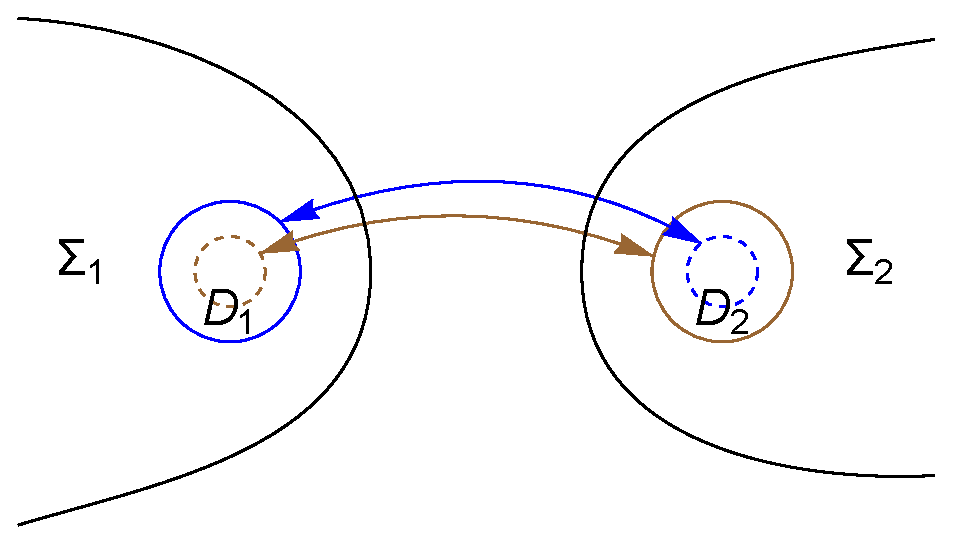
\includegraphics[width=.5\textwidth]{figures/plumbing.pdf}
\caption{The plumbing fixture that joins a pair of Riemann surfaces $\Sigma_1$, $\Sigma_2$. The discs inside the dotted circles within $D_1$ and $D_2$ are removed, whereas the annuli in between the solid and dotted circles are identified via (\ref{gluingmapzz}).}\label{fig:plumbing}
\end{figure}

Equivalently, we may work with the cylinder coordinate $w$, related to $z$ by $z = e^{-i w}$, and similarly $w'$ related to $z'$ by $z' = e^{-i w'}$, and express the map (\ref{gluingmapzz}) as
\ie
w' = -2\pi \tau - w
\fe
where $q\equiv e^{2\pi i \tau}$. $\Sigma(q)$ is obtained by joining $\Sigma_1\backslash D_1$ and $\Sigma_2\backslash D_2$ to the two ends of a cylinder of circumference $2\pi$ and length $-\log|q|$ parameterized by $w$, via the identification $z=e^{-iw}$ at $|z|=1$ and $z' = q e^{i w}$ at $|z'|=1$.

The degeneration limit corresponds to $q\to 0$, which lies on the boundary of the moduli space of $\Sigma$. Near the degeneration limit, $\Sigma$ may be constructed as $\Sigma(q)$ by the plumbing fixture introduced above, and a neighborhood of the boundary of the moduli space may be identified with ${\cal M}_{g_1, n_1}\times {\cal M}_{g_2, n_2}\times \{q: |q|<1\}$.\footnote{Strictly speaking, this identification depends on additional data, namely how the coordinates $z$ on $D_1\subset \Sigma_1$ and $z'$ on $D_2\subset \Sigma_2$ are chosen as the moduli of $\Sigma_1$ and $\Sigma_2$ vary over ${\cal M}_{g_1, n_1}$ and ${\cal M}_{g_2, n_2}$ respectively.  } The contribution from the moduli integration in this domain to the amplitude (\ref{omegaone}) takes the form
\ie\label{ampnearxxb}
& N_{h,n} \int_{{\rm Im}(\tau)>0} d\tau \wedge d\bar\tau \, \langle\langle S_2 |{\cal B}_{\bar\tau} {\cal B}_\tau\, q^{L_0} \bar q^{\widetilde L_0} | S_1 \rangle .
\fe
Here ${\cal B}_\tau$ is the $b$ ghost insertion (\ref{bkfactor}) associated with the modulus $\tau$, explicitly
\ie\label{batauzero}
{\cal B}_{\tau} = \oint {dz\over 2\pi i} b_{zz} \left.{\partial z\over \partial \tau}\right|_{z'}= \oint {dz\over 2\pi i} b_{zz} (2\pi i z)  = 2\pi i b_0,
\fe
where $b_0$ is viewed as an operator that acts on a state that propagates through the cylinder. Likewise, we can write ${\cal B}_{\bar\tau} = -2\pi i \widetilde b_0$. $|S_i\rangle$ is the ``surface state'' produced by the matter+ghost CFT on $\Sigma_i\backslash D_i$ with the insertion of the appropriate $n_i-1$ vertex operators and the $b$ ghosts as in the prescription for the differential form $\Omega$ (\ref{omegatwo}), integrated over ${\cal M}_{g_i, n_i}$. $\langle\langle S_2|$ is the BPZ conjugate of $|S_2\rangle$. Finally, the insertion of $q^{L_0} \bar q^{\widetilde L_0}$ in (\ref{ampnearxxb}) is due to the propagation of the CFT state along the cylinder,  by Euclidean time $2\pi {\rm Im}(\tau)$ and spatial twist $2\pi {\rm Re}(\tau)$.
Evaluating the $(\tau,\bar\tau)$-integral in (\ref{ampnearxxb}) gives the result\footnote{A factor $-2i$ arises due to the integration measure defined through the differential form $d\tau\wedge d\bar\tau=-2i d{\rm Re}(\tau) \wedge d{\rm Im}(\tau)$.}
\ie\label{foupiss}
-4\pi i N_{h,n} \langle\langle S_2 | \widetilde b_0 b_0 { \delta_{L_0, \widetilde L_0}\over L_0 + \widetilde L_0} | S_1 \rangle.
\fe
By an argument similar to (\ref{omegapbrstvar}), the surface state $|S_i\rangle$ is $Q_B$-closed up to possible contributions from the boundary of ${\cal M}_{g_i,n_i}$ which we will for now ignore. Note however that $|S_i\rangle$ does not obey the Siegel constraint and does not represent a physical string state. We can decompose 
\ie\label{psilldec}
\delta_{L_0, \widetilde L_0}| S_1\rangle = \sum_\C |\Phi_\C(P)\rangle,
\fe
where $|\Phi_\C(P)\rangle$ are eigenstates of $L_0$ and $\widetilde L_0$ that carries spacetime momentum $P^\mu$, the latter being equal to the sum of the spacetime momenta of the $n_1-1$ vertex operators inserted on $\Sigma_1\backslash D_1$, such that
\ie
L_0 |\Phi_\C(P)\rangle = \widetilde L_0 |\Phi_\C(P)\rangle = {\A'\over 4} \left( P^2 + M_\C^2\right) |\Phi_\C(P) \rangle.
\fe
For the free boson matter CFT, $M_\C^2={4\over \A'}(N_\C-1)$ where $N_\C$ is the oscillator level of $|\Phi_\C(P)\rangle$, and in particular does not vary with the spacetime momenta.

\subsubsection{Factorization of the string amplitude}
\label{sec:factorbos}

As $P^2$ approaches $-M_\C^2$, (\ref{ampnearxxb}) gives rise to a pole in the string amplitude, of the form
\ie\label{psimfac}
-{8\pi i N_{h,n} \over \A' (P^2+M_\C^2)} \langle\langle S_2|\widetilde b_0 b_0 | \Phi_\C(P) \rangle.
\fe
When $P^2=-M_\C^2$, $|\Phi_\C(P)\rangle$ is annihilated by $L_0$ and $\widetilde L_0$. In this case, the state $\widetilde b_0 b_0 |\Phi_\C(P)\rangle$ is $Q_B$-closed and also obey the Siegel constraint, and therefore represents a physical string state. Without loss of generality, we may assume that  the BRST cohomology class of $\widetilde b_0 b_0 |\Phi_\C(P)\rangle$ at $P^2=-M_\C^2$ is proportional to that of $|{\cal V}_\C(P)\rangle$, where ${\cal V}_\C(P)=c\widetilde c V_\C(P)$ is an OCQ representative appropriately normalized as 
\ie\label{vvnormvonv}
\langle\langle \overline{\cV_\C(P)}| c_0 \widetilde c_0|\cV_{\C'} (P')\rangle = {K_{S^2}}\delta_{\C\C'} i(2\pi)^{D} \delta^{D}( P- P'),
\fe
where $\overline{{\cal V}_\C(P)}\equiv c\widetilde c \overline{V_\C(P)}$, $\overline{V_\C(P)}$ being the Hermitian conjugate of the matter CFT operator $V_\C(P)$, and $K_{S^2}$ is a constant to be fixed below. Inserting $\overline{\cV_\C(P')}$ for an on-shell momentum $P'^\mu$ at the puncture $z=0$ on $\Sigma_1$ yields a genus $g_1$, $n_1$-string amplitude
\ie\label{noneamcs}
N_{g_1,n_1} \langle\langle \overline{\cV_\C(P')} |S_1 \rangle = i (2\pi)^D \delta^D(P-P') \widehat {\cal A}_{g_1}[\overline{V_\C(P')}, \cdots],
\fe
where $\cdots$ stands for the remaining $n_1-1$ vertex operators on $\Sigma_1$. It follows from (\ref{psilldec}), (\ref{vvnormvonv}), and (\ref{noneamcs}) that
\ie\label{phigama}
\left. \widetilde b_0 b_0 |\Phi_\C(P)\rangle\right|_{P^2=-M_\C^2} =  N_{g_1,n_1}^{-1} K_{S^2}^{-1} \widehat {\cal A}_{g_1}[\overline{V_\C(P)}, \cdots] \, |\cV_\C(P)\rangle .
\fe
Likewise, inserting $\cV_\C(P')$ at $z'=0$ on $\Sigma_2$ yields a genus $g_2$, $n_2$-string amplitude
\ie\label{ntwoamcs}
N_{g_2,n_2} \langle\langle S_2 | \cV_\C(P')\rangle = i(2\pi)^D \delta^D(P-P') \widehat {\cal A}_{g_2}[\cdots, V_\C(P')].
\fe
Comparing (\ref{phigama}), (\ref{ntwoamcs}) with (\ref{psimfac}), we see that the residue of the amplitude with respect to $P^2$ at $P^2=-M_\C^2$ is equal to
\ie\label{onshellgfact}
-{8\pi i N_{h,n} \over \A' N_{g_1,n_1} N_{g_2,n_2} K_{S^2}} \widehat {\cal A}_{g_1}[\cdots, V_\C(P)]\cdot \widehat {\cal A}_{g_2}[\overline{V_\C(P)}, \cdots].
\fe
This is precisely the factorization relation expected from unitarity analogous to (\ref{ampfactorization}), provided that the normalization factors obey
\ie\label{nexpresa}
N_{g_1,n_1} N_{g_2,n_2} = - i N_{h,n} {8\pi  \over \A' K_{S^2}} ,
\fe
where $h=g_1+g_2$ and $n=n_1+n_2-2$. 

A similar consideration of the degeneration limit where one of the handles of $\Sigma$ pinches off leads to the normalization condition
\ie\label{nexpresb}
N_{h-1,n+2} = -i N_{h,n} {8\pi  \over \A' K_{S^2}}.
\fe
We will make the consistent choice
\ie\label{normconsts}
N_{h,n} =i^{3h-3+n},~~~~ K_{S^2} = {8\pi\over \A'}.
\fe
Let us further note that the LHS of (\ref{vvnormvonv}) is given by a sphere two-point function of the worldsheet CFT, which acquires a factor $e^{-2\phi_0}$ if we include the constant dilaton term (\ref{topact}) in the worldsheet action. The normalization condition (\ref{vvnormvonv}) thus requires the vertex operator $V_\C(P)$ to be proportional to $e^{\phi_0}$. We will henceforth define $g_s \equiv e^{\phi_0}$ as the string coupling, and adopt the following normalization of the matter CFT sphere correlator %\footnote{This differs from (6.6.8) of Polchinski by a factor $-i$, due to our convention for the moduli integration measure $d\tau d\bar\tau$ defined as a 2-form in (\ref{ampnearxxb}).} 
\ie\label{eikxcorrconv}
\left\langle e^{ik\cdot X} \right\rangle_{\rm m} = i (2\pi)^D \delta^D(k) g_s^{-2} K_{S^2},
\fe
in addition to the ghost correlator normalization convention of (\ref{ccoresign}). Comparison with (\ref{vvnormvonv}) then fixes the normalization of the string vertex operator. For instance, the closed string tachyon vertex operator $V_T(P)$ is
\ie\label{tachyonvert}
V_T(P) = g_s e^{iP\cdot X}.
\fe



\subsection{Tree-level amplitudes in critical bosonic string theory}
\label{bostree}

The tree-level or genus zero scattering amplitudes in the critical bosonic string theory are well-defined and satisfy the unitarity relation (\ref{ampfactorization}) despite the presence of the closed string tachyon. It is instructive to consider the genus zero $n$-tachyon amplitude ($n\geq 3$),
\ie\label{ainttach}
{\cal A}_0[V_T(k_1), \cdots, V_T(k_n)] = i^{n-3} \int_{{\cal M}_{0,n}} \Omega_{2n-6}
\fe
where ${\cal M}_{0,n}$, the moduli space of the $n$-punctured Riemann sphere, may simply be parameterized by the coordinates of $n-3$ punctures, say $z_4, \cdots, z_n$, unconstrained and taking value over the entire complex plane, while the remaining three punctures are fixed at $z_1, z_2, z_3$. In the construction of $\Omega_{2n-6}$ via (\ref{omegatwo}), the $b$ ghost insertions appear in combination (\ref{ubbvex}) with the tachyon vertex operators at $z_4,\cdots, z_n$ and effectively strips off the $c\widetilde c$ ghosts of the latter via (\ref{intverta}). Using the tachyon vertex operator (\ref{tachyonvert}), we can express the form $\Omega_{2n-6}$ explicitly as a correlator of the worldsheet CFT on the Riemann sphere
\ie\label{omageac}
\Omega_{2n-6} = g_s^n \left\langle \prod_{i=1}^3 c(z_i)\widetilde c(\bar z_i) e^{ik_i\cdot X(z_i, \bar z_i)} \prod_{j=4}^n e^{ik_j\cdot X(z_j,\bar z_j)}  dz_j d\bar z_j \right\rangle,
\fe
which is then evaluated using (\ref{ccoresign}), (\ref{eikxcorrconv}), and the free boson OPE to
\ie\label{tachyonampint}
 i (2\pi)^{26} \delta^{26}\Big(\sum_{i=1}^n k_i\Big) g_s^{n-2} K_{S^2} \prod_{1\leq a< b\leq 3} |z_{ab}|^2 \prod_{1\leq i< j\leq n} |z_{ij}|^{\A' k_i\cdot k_j} \prod_{j=4}^n  dz_j d\bar z_j,
\fe
where $K_{S^2}$ is given by (\ref{normconsts}). The expression (\ref{tachyonampint}) may appear perplexing at first sight as it depends explicitly on the arbitrarily chosen points $z_1, z_2, z_3$. We should also keep in mind that the momenta $k_i$ of the tachyon vertex operators are subject to the mass-shell condition $k_i^2 = -m_T^2= {4\over \A'}$. Taking into account the mass-shell condition as well as the momentum conservation enforced by the delta function in (\ref{tachyonampint}), one can indeed verify that $\Omega_{2n-6}$ is covariant with respect to the $PSL(2,\mathbb{C})$ M\"obius transformation (\ref{ckgelm}) on the $z_i$'s, and consequently the amplitude obtained by integration over $\cM_{0,n}$ is independent of $z_1, z_2, z_3$. As already anticipated in section \ref{stringscatt}, the integral of (\ref{tachyonampint}) is divergent near $z_i=z_j$ if $\A' k_i\cdot k_j \leq -2$, in which case (\ref{ainttach}) should be understood as a regularized integral, defined by either analytic continuation in the momenta of the tachyon vertex operators, or equivalently cutting off a small neighborhood of $z_i=z_j$ and subtracting off power divergences. 

For $n=3$, ${\cal M}_{0,3}$ is one point so there is no integration to do. The 3-tachyon reduced amplitude is read off to be
\ie
\label{threetach}
\widehat {\cal A}_0[V_T(k_1), V_T(k_2), V_T(k_3)] =  {8\pi\over \A'} g_s.
\fe
For $n=4$, ${\cal M}_{0,4}$ is parameterized by a single complex modulus $z_4$, and the 4-tachyon reduced amplitude, known as the Virasoro-Shapiro amplitude, takes the form
\ie
\label{fourtach}
\widehat{\cal A}_0[V_T(k_1), V_T(k_2), V_T(k_3), V_T(k_4)] = {8\pi\over \A'} g_s^2 F(s, t, u),
\fe
where $s=-(k_1+k_2)^2$, $t=-(k_1+k_4)^2$, $u=-(k_1+k_3)^2$ are the Mandelstam variables that obey $s+t+u = 4m_T^2$, and the function $F(s, t, u)$ can be evaluated by setting $z_1=0$, $z_2=1$, $z_3=\infty$ in (\ref{tachyonampint}), giving
\ie\label{jfuncsfu}
F(s, t, u) &= \int id z_4\wedge d\bar z_4\, |z_4|^{\A' k_1\cdot k_4} |1-z_4|^{\A' k_2\cdot k_4}
\\
&= 2\pi {\Gamma(-{\A'\over 4} s - 1) \Gamma(-{\A'\over 4} t - 1) \Gamma(-{\A'\over 4} u - 1) \over \Gamma({\A'\over 4} s+2) \Gamma({\A'\over 4} t+2) \Gamma({\A'\over 4} u+2)}.
\fe
One observes that (\ref{jfuncsfu}) has poles with respect to $s$ at $s = {4\over \A'} n$, $n=-1,0,1,2,\cdots$ (and similarly with respect to $t, u$). These are precisely the mass squared values of closed string states that can appear as intermediate 1-particle states in (\ref{ampfactorization}).

One may attempt to construct an action functional $S$ in 26 dimensions whose field variables are in correspondence, modulo possible gauge redundancy, with the physical string states, such that the tree-level amplitudes that follow from $S$ reproduces the tree-level amplitudes of critical bosonic string theory. For instance, the 3-tachyon amplitude (\ref{threetach}) would be reproduced by a cubic coupling of the tachyon field in the action
\ie\label{sttoy}
S = \int d^{26} x \left[ -{1\over 2}(\partial_\mu T)^2 + {2\over \A'} T^2 + {4\pi\over 3\A'} g_s T^3 + \cdots \right].
\fe
To recover the full action $S$ from the string amplitudes seems like a daunting task, as couplings to arbitrarily high orders in the fields as well as in the spacetime derivatives will appear, and are furthermore subject to the ambiguity of nonlinear field redefinitions. A systematic construction of such an action in the framework of closed string field theory will be introduced in Chapter \ref{sftchap}. For now, let us note that in the long wavelength limit, one may solve the equation of motion of the tachyon as well as the massive fields in terms of the massless fields, namely the metric $G_{\mu\nu}$, 2-form potential $B_{\mu\nu}$, and the dilaton $\Phi$, and reduce $S$ to a massless effective action $S_{\rm eff}[G, B, \Phi]$ that is equivalent to (\ref{treemasslesseff}) up to a field redefinition. Comparison of tree-level amplitude with a graviton emission determines the relation between the gravitational coupling $\kappa$ appearing in (\ref{treemasslesseff}) and the string coupling $g_s$ to be
\ie\label{kapgsbos}
\kappa = 2\pi g_s.
\fe


\subsection{One-loop amplitudes}
\label{sec:oneloop}

%Due to the presence of tachyon, loop amplitudes of the critical bosonic string theory are not expected to be well defined. Nonetheless, it is possible to write down a set of moduli space integrands that are formally consistent with perturbative unitarity. In this and the next section, we will give some explicit examples of the moduli space integrand of closed string loop amplitudes, as a warm-up exercise for our later consideration of well-defined string loop amplitudes (such as in $c\leq 1$ string theory and superstring theory).

We now turn to the 1-loop or genus one string amplitude
\ie\label{tachnaloo}
{\cal A}_1[V_1(k_1),\cdots,V_n(k_n)] = i^n \int_{{\cal M}_{1,n}} \Omega_{2n},
\fe
where ${\cal M}_{1,n}$, the moduli space of the $n$-punctured torus, can be parameterized by the torus modulus $\tau$ together with the coordinates $z_2, \cdots, z_n$ of $n-1$ puncture, leaving the remaining one puncture fixed at $z_1=0$. The modulus $\tau$ may be taken to be valued in the fundamental domain with respect to $PSL(2,\mathbb{Z})$ (see Appendix \ref{torussec})
\ie\label{funddomaintor}
{\cal F} =\Big\{\tau\equiv\tau_1+i\tau_2:~ | \tau_1 | \leq {1\over 2},~\tau_2>0, ~|\tau|\geq 1 \Big\},
\fe
while each of $z_2,\cdots,z_n$ is subject to the periodic identification
\ie
z_i \sim z_i + 2\pi \sim z_i + 2\pi \tau.
\fe
In addition, we must also take into account overall $\mathbb{Z}_2$ identification
\ie\label{ztwoid}
(\tau; z_2,\cdots,z_n) \sim (\tau; -z_2,\cdots,-z_n)
\fe
due to the residual $\mathbb{Z}_2$ conformal Killing group unfixed by the choice of the puncture at $z_1=0$.

\begin{figure}[h!]
\centering
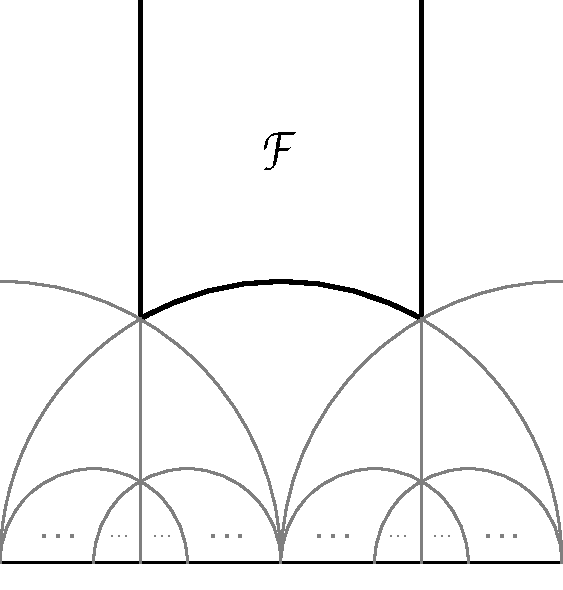
\includegraphics[width=.35\textwidth]{figures/funddomain.pdf}
\caption{The fundamental domain ${\cal F}$, enclosed by the solid black lines, and its $PSL(2,\mathbb{Z})$ images that tile the upper half complex $\tau$-plane.}\label{fig:funddomain}
\end{figure}

In constructing the degree $2n$ form $\Omega_{2n}$, we may use $2n-2$ of the $b$ ghost insertions associated with the moduli $z_2,\cdots, z_n$ to eliminate the $c\widetilde c$ ghost in $n-1$ of the vertex operators. The remaining pair of $b$ ghost insertions, associated with the moduli $(\tau,\bar\tau)$, may be expressed using (\ref{batauzero}) as simply
\ie
{\cal B}_\tau = - i \oint dz \, b(z), ~~~~ {\cal B}_{\bar \tau} = i \oint d\bar z\, \widetilde b(\bar z),
\fe
where the integration contour is along spatial circle of the torus (of circumference $2\pi$). $\Omega_{2n}$ is then given by the torus correlator
\ie\label{torusintegrands}
\Omega_{2n} =  \left\langle d\tau d\bar\tau {\cal B}_{\bar\tau} {\cal B}_\tau \, c\widetilde c V_1(0) \prod_{i=2}^n V_i(z_i,\bar z_i)  dz_i d\bar z_i \right\rangle_{T^2(\tau)}.
\fe
To proceed, let us note that the torus correlator of $\widetilde b b c \widetilde c$ is independent of the coordinates of the $b$ and $c$ ghost insertions, as only the constant modes of the latter contributes to the functional integral of the $bc$ system on the torus. Explicitly, the ghost correlator can be evaluated as
\ie\label{bbcctor}
\big\langle  \widetilde b b c \widetilde c \big\rangle_{T^2(\tau)} &= {\rm Tr}_{{\cal H}_{\rm gh}} (-)^{N_{\rm gh}} \widetilde b_0 b_0 c_0 \widetilde c_0 q^{L_0 - {c_{\rm gh}\over 24}} \widetilde q^{\widetilde L_0 - {c_{\rm gh}\over 24}}
\\
&= \left| q^{1\over 12} \prod_{n=1}^\infty (1-q^n)^2\right|^2 = |\eta(\tau)|^4.
\fe
Here ${\cal H}_{\rm gh}$ is the space of states of the $bc$ system, $N_{\rm gh}$ is the total left and right ghost number, $c_{\rm gh}=-26$ is the central charge of the $bc$ system, and we have defined $q\equiv e^{2\pi i \tau}$. We can further average the position of the vertex operator $V_1$ over the torus using the translation invariance, and write the 1-loop amplitude (\ref{tachnaloo}) as
\ie\label{modulioneloopinte}
{\cal A}_1[V_1(k_1),\cdots,V_n(k_n)] = {1\over 2} \int_{\cal F} {i d \tau \wedge d\bar\tau\over 2\tau_2} |\eta(\tau)|^4 \left\langle \prod_{i=1}^n \int_{T^2(\tau)} i dz_i \wedge d\bar z_i\, V_i(z_i, \bar z_i) \right\rangle_{{\rm m}, T^2(\tau) },
\fe
where all $n$ vertex operators are treated on equal footing. On the RHS, the overall factor ${1\over 2}$ is due to the $\mathbb{Z}_2$ identification (\ref{ztwoid}) in our parameterization of the moduli space ${\cal M}_{1,n}$, and the factor ${1\over 2\tau_2}$ serves to cancel against a volume factor that arises from the $z_1$-integral.

The prescription (\ref{tachnaloo}) requires the number of punctures $n$ to be at least 1. For $n\geq 3$, (\ref{modulioneloopinte}) amounts to the 1-loop contribution to a scattering amplitude. The $n=2$ case may be viewed as a 1-loop renormalization of the 1-particle state. The $n=1$ case arises only at zero momentum and would be on-shell only for a massless string state, in which case it amounts to a massless tadpole that, if non-vanishing, would signify the breakdown of perturbation theory as the spacetime background would not be a true vacuum configuration.

The formula (\ref{modulioneloopinte}) also admits an obvious generalization to the $n=0$ case, which by analogy with perturbative quantum field theory should admit the interpretation as a 1-loop contribution to the spacetime vacuum energy density multiplied by the (divergent) spacetime volume. Indeed, we may write
\ie\label{aoneform}
{\cal A}_1 = {1\over 2} \int_{\cal F} {i d \tau \wedge d\bar\tau\over 2\tau_2} |\eta(\tau)|^4 Z_{\rm m}(\tau, \bar\tau),
\fe
where $Z_{\rm m}$ is the torus partition function of the matter CFT. As a sanity check, note that the integrand on the RHS is invariant under the $PSL(2,\mathbb{Z})$ transformation of the modulus $\tau$ (\ref{psltz}), and so the integral is independent of the choice of the fundamental domain ${\cal F}$ with respect to $PSL(2,\mathbb{Z})$ on the upper half complex $\tau$-plane.

In the case of critical bosonic string theory, the torus partition function of the matter CFT evaluates to
\ie
Z_{\rm m}(\tau, \bar\tau) = i V_X \int {d^{26} k_E \over (2\pi)^{26}} e^{- \pi \A' k_E ^2 \tau_2} |\eta(\tau)|^{-52},
\fe
where $V_X$ is the Minkowskian spacetime volume, $k_E$ stands for a Euclidean 26-dimensional momentum vector, and the overall factor of $i$ comes from the Wick rotation of the momentum integration contour. The exponential growth of $Z_{\rm m}(\tau, \bar\tau)$ in the $\tau_2\to \infty$ limit leads to a divergent moduli integral on the RHS of (\ref{aoneform}). After all, the critical bosonic string theory is not expected to admit a well-defined quantum perturbation theory due to the closed string tachyon.

A more interesting example is $c=1$ string theory at finite temperature $1/\B$, which may be described by the worldsheet matter CFT that consists of a compact boson $X$ of radius $R={\B\over 2\pi}$, and the $c=25$ Liouville theory. The torus partition function of this matter CFT evaluates to
\ie\label{zmtherm}
Z_{\rm m}(\tau, \bar\tau) = V_\phi \int_0^\infty {dP\over \pi} e^{- \pi \A' P^2 \tau_2} \sum_{n, w\in\mathbb{Z}} e^{- \pi\tau_2 \left( {\A' n^2\over R^2} + {w^2 R^2\over \A'} \right) + 2\pi i \tau_1 n w }  |\eta(\tau)|^{-4},
\fe
where $P$ is the Liouville momentum, $V_\phi$ is the (divergent) length of the target space of the Liouville field $\phi$, and $n, w$ are the momentum and winding quantum numbers with respect to the thermal circle. Plugging (\ref{zmtherm}) into (\ref{aoneform}), after canceling the $\eta$-function factors and performing a Poisson resummation with respect to $n$, we can express the resulting 1-loop vacuum amplitude as
\ie\label{aonerigs}
{\cal A}_1 = {V_\phi R\over 4\pi \A'} \int_{\cal F} {i d \tau \wedge d\bar\tau\over 2\tau_2^2} \sum_{\widetilde n, w\in\mathbb{Z}} e^{- {\pi R^2\over \A' \tau_2} |\widetilde n-w\tau|^2 }.
\fe
The sum and integration on the RHS can be simplified with the following rearrangement: for the summand labeled by $(\widetilde n, w)\not=(0,0)$, let $k={\rm gcd}(\widetilde n, w)$, $a=\widetilde n/k$, $c=w/k$. As the integers $a$ and $c$ are coprime, we can find integers $b, d$ such that $ad-bc=1$, and consider the $PSL(2,\mathbb{Z})$ transformation $\tau\mapsto (a\tau+ b)/(c\tau + d)$ under which the summand on the RHS of (\ref{aonerigs}) transforms by 
\ie
e^{- {\pi R^2\over \A' \tau_2} |\widetilde n-w\tau|^2 } \mapsto e^{- {\pi R^2\over \A' \tau_2} k^2 }.
\fe
Such a $PSL(2,\mathbb{Z})$ transformation maps the domain ${\cal F}$ to another fundamental domain within the strip $|\tau_1|\leq {1\over 2}, \tau_2>0$, and the collection of the images under such transformations cover the entire strip. In the end, (\ref{aonerigs}) can be rewritten and evaluated as
\ie
{\cal A}_1 &=  {V_\phi R\over 4\pi \A'} \left( \int_{\cal F} {i d \tau \wedge d\bar\tau\over 2\tau_2^2} + 2\sum_{k=1}^\infty \int_{|\tau_1|\leq {1\over 2},\tau_2>0} {i d \tau \wedge d\bar\tau\over 2\tau_2^2}  e^{- {\pi R^2\over \A' \tau_2} k^2 } \right)
\\
&= {V_\phi \over 12} \left( {R\over \A'} + {1 \over R} \right).
\fe
As a consistency check, the result is invariant under the T-duality of the thermal circle $R\to \A'/R$. The term proportional to $R$ can be interpreted as a constant contribution to the vacuum energy density in the asymptotic region of the target space, whereas the term proportional to $1/R$ amounts to a thermal free energy
\ie\label{fbfree}
F(\B) = V_\phi {\pi \over 6 \B}.
\fe
This precisely agrees with the thermal free energy of a free massless boson field in 1+1 dimensions, as expected from the physical string states of $c=1$ string theory in the asymptotic region.

\subsection{Higher loops}
\label{sec:boshigherloop}

We now turn to the string amplitude at genus $h\geq 2$,
\ie
{\cal A}_h[V(k_1), \cdots, V(k_n)] = i^{3h-3+n} \int_{{\cal M}_{h,n}} \Omega_{6h-6+2n}, 
\fe
where ${\cal M}_{h,n}$ may be viewed as a fibration over the moduli space ${\cal M}_h$ of a genus $h$ Riemann surface $\Sigma$ without puncture, whose fiber is parameterized by the coordinates $z_1, \cdots, z_n$ of the $n$ punctures on $\Sigma$. As seen in Appendix \ref{sec:ggttwors}, ${\cal M}_h$ is itself a complex space that can be parameterized by holomorphic moduli $\tau^1, \cdots, \tau^{3h-3}$, whose corresponding ${\cal B}_{\tau_k}$ involves only the holomorphic $b$ ghost. We can therefore write the differential form $\Omega_{6h-6+2n}$ as
\ie\label{omegadetex}
\Omega_{6h-6+2n} &=  \left\langle \prod_{k=1}^{3h-3} d\tau^k d\bar\tau^k {\cal B}_{\bar\tau_k}{\cal B}_{\tau_k}  \prod_{i=1}^n V_i(z_i,\bar z_i) d z_i d\bar z_i \right\rangle_\Sigma.
\fe
%Formally, (\ref{omegadetex}) factorizes into the holomorphic ghost, the anti-holomorphic ghost, and the matter CFT correlators. Note however that the ghost and matter correlators separately depend the choice of a Hermitian metric on $\Sigma$ due to their Weyl anomaly, and moreover the holomorphic ghost CFT by itself is subject to a gravitational anomaly. All of these anomalies are expected to cancel in the full worldsheet CFT correlator (\ref{omegadetex}).

A priori, correlators on a higher genus Riemann surface may be calculated either by cutting and sewing as described in Appendix \ref{modularsec}, or by directly evaluating the path integral. The former approach can be streamlined using Virasoro conformal blocks and makes use of only the spectrum and structure constants intrinsic to the CFT, whereas the latter approach is more convenient for free field theories and renders more apparent global properties of the moduli space such as modular invariance. 

In the $bc$ system, it is possible to determine the correlation functions by a combination of OPE, modular invariance, and holomorphy considerations. The full results will be described in section \ref{sec:bchigherg}. For now we illustrate with the genus $h=2$ example, where a number of simplifications occur. To begin with, note that the genus two moduli space ${\cal M}_2$ can be parameterized by the period matrix $\Omega_{IJ}$, taking value over the Siegel upper half space ${\rm Im}\Omega\succ 0$, subject to identification with respect to the $Sp(4,\mathbb{Z})$ transformation
\ie\label{omegaspf}
\Omega\mapsto \Omega' = (A\Omega+B)(C\Omega + D)^{-1},
\fe
where the matrices $A,B,C,D$ are defined as in (\ref{abcdmat}).
Let $\omega_I = \omega_I(z)dz$, $I=1,2$ be a basis of holomorphic 1-forms on a genus two Riemann surface $\Sigma$, normalized as in (\ref{holoneformnorm}), (\ref{periodmatdef}) in relation to the period matrix. The zero modes of $b(z)$, in correspondence with holomorphic quadratic differentials on $\Sigma$, can be expressed as a linear combination of $S_{1,2,3}$, where
\ie
S_{1}(z) = (\omega_1(z))^2, ~S_2(z) = (\omega_2(z))^2,~S_3 = \omega_1(z) \omega_2(z).
\fe
It follows from the general structure of the Grassmann functional integral of the $bc$ system that the correlator of three pairs of $b$ and $\widetilde b$ ghosts on $\Sigma$ receives contribution from only the zero modes of the ghost insertions,
\ie\label{bghgentwo}
\Big\langle \left| b(z_1) b(z_2) b(z_3) \right|^2 \Big\rangle_{\Sigma} = f(\Sigma) \left| \det (S_i(z_j)) \right|^2  ,
\fe
where $ f(\Sigma)$ is independent of $z_1, z_2, z_3$, but depends on the moduli of $\Sigma$ as well as a choice of Hermitian metric on $\Sigma$ due to the Weyl anomaly of the $bc$ system.
%\ie
%\Delta(z_1, z_2) \Delta(z_2, z_3) \Delta(z_3, z_1)
%\fe
%where $\Delta(z_1,z_2) \equiv \omega_1(z_1)\omega_2(z_2)-\omega_1(z_2)\omega_2(z_1)$. To determine the remaining moduli dependence, 
Integrating (\ref{bghgentwo}) against the Beltrami differentials (\ref{beltramidif}) and using the identity
\ie
{\partial\Omega_{IJ}\over \partial \tau^k} = \int d^2z\, \omega_I(z) \omega_J(z) (\mu_k)_{\bar z}{}^z(z,\bar z),
\fe
where $\mu_k$ is defined as in (\ref{beltramidif}) with $t^k$ replaced by the holomorphic modulus $\tau^k$, we obtain 
\ie\label{dtkaa}
\left\langle\prod_{k=1}^{3} d\tau^k d\bar\tau^k {\cal B}_{\bar\tau^k} {\cal B}_{\tau^k} \right\rangle_\Sigma =  f(\Sigma) |d\Omega_{11}d\Omega_{22}d\Omega_{12}|^2 .
\fe
For the critical bosonic string theory, the genus two vacuum amplitude has formally the moduli space integrand
\ie\label{omegasix}
\Omega_6 = f(\Sigma) Z_X(\Sigma) |d\Omega_{11}d\Omega_{22}d\Omega_{12}|^2 ,
\fe
where $Z_X(\Sigma)$ is the partition function of the 26 free bosons $X^\mu$ on $\Sigma$. A priori, $Z_X(\Sigma)$ also depends on the choice of Hermitian metric on $\Sigma$, but the combination $f(\Sigma) Z_X(\Sigma)$ should be Weyl invariant.

In principle, we can also construct (\ref{omegasix}) using holomorphic conformal blocks of the ghost and matter CFT, which gives rise to
\ie\label{fzxform}
f(\Sigma) Z_X(\Sigma) = V_X {g_s^2 \A'\over 8\pi} \int \prod_{I=1,2} {d^{26} k_I\over (2\pi)^{26}} e^{-\pi \A' \sum_{I,J}  k_I\cdot k_J{\rm Im}\Omega_{IJ} } | \Phi(\Omega)|^2,
\fe
where $V_X$ is the spacetime volume due to the integration over the zero modes of $X^\mu$, $k_I^\mu = {1\over \pi \A'} \oint_{\A^I} dz \partial X^\mu$ is the spacetime momentum flowing through the $\A^I$ 1-cycle on $\Sigma$, $\Phi(\Omega)$ is the contribution from holomorphic oscillators of the $bc$ ghosts and 26 free bosons, and depends holomorphically on $\Omega_{IJ}$. Evaluating the $k_I$-integrals by Wick rotation, we arrive at
\ie\label{omegasixex}
\Omega_6 = - {V_X\over (4\pi^2\A')^{26} (\det {\rm Im}\Omega)^{13}} \left| \Phi(\Omega) d\Omega_{11}d\Omega_{22}d\Omega_{12}\right|^2.
\fe
Modular invariance with respect to (\ref{omegaspf}) dictates that $\Phi(\Omega)$ must transform according to
\ie\label{phimodular}
\Phi(\Omega') = \det(C\Omega+D)^{-10} \Phi(\Omega).
\fe
Furthermore, $\Phi(\Omega)$ is nowhere vanishing on the Siegel upper half space, and has poles only on the boundary of the moduli space where the Riemann surface $\Sigma$ degenerates. An example of the degeneration limit is $\Omega_{12}\to 0$, where $\Sigma$ pinches into a pair of tori, of moduli $\Omega_{11}$ and $\Omega_{22}$ respectively, joined by the plumbing fixture (\ref{gluingmapzz}) with the sewing parameter $q\approx 2\pi i \Omega_{12}$. In this limit, $\Phi(\Omega)$ is 
dominated by the contribution from the oscillator ground state, of weight $L_0=-1$, propagating through the plumbing fixture, giving
\ie\label{phideg}
\Phi(\Omega) d\Omega_{11}d\Omega_{22}d\Omega_{12} \to {dq\over q^2}{d\Omega_{11} \over (\eta(\Omega_{11}))^{24} }{d\Omega_{22}\over( \eta(\Omega_{22}))^{24}}.
\fe
The modular and analytic properties together with the degeneration limit (\ref{phideg}) determines $\Phi(\Omega)$ uniquely to be
\ie
\Phi(\Omega) = {2\pi i\over \chi_{10}(\Omega)},
\fe
where $\chi_{10}$ is known as the Igusa cusp form.\footnote{Explicitly,  $\chi_{10}$ admits a product representation
\ie
\chi_{10}(\Omega) = e^{2\pi i (\Omega_{11}+\Omega_{22}+\Omega_{12})} \prod_{(k,\ell,m)>0} \left( 1 - e^{2\pi i (k\Omega_{11}+\ell \Omega_{22}+m \Omega_{12})} \right)^{c(4kl-m^2)},
\fe
where the notation $(k,\ell,m)>0$ means that the product is taken over integers $k,\ell,m$ with either $k,\ell>0$ and $m$ unrestricted, or $k=\ell=0$ and $m<0$. The exponents $c(n)$ are non-vanishing only when $n\geq -1$ and $n\equiv -1, 0$ mod 4, with the first few cases given by $c(-1) = 2$, $c(0)=20$, $c(3)=-128$, $c(4)=216$.}

The moduli space integral of (\ref{omegasixex}) is unsurprisingly divergent due to the propagation of the closed string tachyon. Nonetheless, we can apply the same strategy to compute a well-defined 2-loop vacuum amplitude of the $c=1$ string theory, simply by multiplying the RHS of (\ref{omegasixex}) with the Weyl-invariant ratio of partition functions $Z_{X^0}(\Sigma)Z_L(\Sigma)/Z_X(\Sigma)$, where $Z_{X^0}(\Sigma)$ is the partition function of the timelike free boson and $Z_L(\Sigma)$ that of the $c=25$ Liouville theory on the genus two surface $\Sigma$.


\subsection{Scattering amplitudes in $c=1$ string theory}
\label{conetree}

The $c=1$ string theory, whose worldsheet CFT is described in section \ref{conesec}, has a 1+1 dimensional target spacetime with only time and not space translation invariance. We will denote by $|\omega\rangle^{\rm in/out}$ the in/out state of a single closed string of energy $\omega\over\sqrt{\A'}$, with the normalization convention
\ie\label{conenorm}
{}^{\rm in}\langle\omega|\omega'\rangle{}^{\rm in} ={}^{\rm out}\langle\omega|\omega'\rangle{}^{\rm out} = \omega\, \delta(\omega - \omega').
\fe
The corresponding vertex operator in the worldsheet description is
\ie
{\cal V}_\omega^\pm = g_s c\wt c e^{\pm i{\omega\over \sqrt{\A'}} X^0} V_{P={\omega\over 2}},
\fe
where the sign $+/-$ labels in/out states, and $V_P$ is the Liouville primary defined as (\ref{vvin}) and normalized according to (\ref{vpnormvp}). Analogously to (\ref{eikxcorrconv}), the sphere correlator in the $X^0$ CFT takes the form
\ie
\left\langle e^{-i k^0 X^0} \right\rangle_{X^0} = 2\pi i \delta(k^0) g_s^{-2} \wt K_{S^2},
\fe
where the normalization constant $\wt K_{S^2}$ is determined by the unitarity relations to be
\ie\label{wtkstwo}
\wt K_{S^2} = {2\over \sqrt{\A'}}.
\fe
We now consider the $1\to n$ S-matrix element, with an in-particle of energy $\omega$ and out-particles of energy $\omega_1, \cdots, \omega_n$, of the form
\ie\label{sacone}
S(\omega_1, \cdots, \omega_n; \omega) = \delta\Big( \omega - \sum_{i=1}^n \omega_i \Big) {\cal A}(\omega_1,\cdots,\omega_n).
\fe
The amplitude ${\cal A}$ admits the genus expansion
\ie
{\cal A}(\omega_1,\cdots,\omega_n) = \sum_{h=0}^\infty {\cal A}_h(\omega_1,\cdots,\omega_n),
\fe
where ${\cal A}_h$ is of order $g_s^{2h + n - 1}$, and is moreover subject to the (perturbative) unitarity relation 
\ie
\sum_{n=1}^\infty \int_{\omega_i> 0} \prod_{i=1}^n {d\omega_i}\, \delta\Big( \omega - \sum_{i=1}^n \omega_i \Big) { |{\cal A}(\omega_1,\cdots,\omega_n)|^2\over \omega \omega_1\cdots\omega_n} = 1.
\fe
As the simplest nontrivial example, the tree-level $1\to 2$ S-matrix element is
\ie
S(\omega_1, \omega_2; \omega) &= \left\langle {\cal V}_\omega^+ {\cal V}_{\omega_1}^- {\cal V}_{\omega_2}^- \right\rangle
\\
&= i g_s \wt K_{S^2} 2\pi \sqrt{\A'} \delta(\omega-\omega_1-\omega_2) {\cal C}(\tfrac{\omega}{ 2},\tfrac{\omega_1}{ 2},\tfrac{\omega_2}{ 2}),
\fe
where ${\cal C}(P_1, P_2, P_3)$ is the Liouville structure constant appearing in (\ref{vvvcppp}). For the $c=25$ Liouville CFT, the structure constant is given by the $b\to 1$ limit of (\ref{dozz}), which can be written as
\ie
{\cal C}(P_1, P_2, P_3) = {1\over \Upsilon_1(1 + i(P_1+P_2+P_3))} \left[ { 2P_1 \Upsilon_1(1+2iP_1)\over \Upsilon_1(1 + i(P_2+P_3-P_1)) } \times (2~{\rm permutations}) \right].
\fe
In the case $P_3=P_1+P_2$, using $\Upsilon_1(1)=1$, the formula simplifies dramatically to
\ie
{\cal C}(P_1, P_2, P_1+ P_2 ) = 8 P_1 P_2 (P_1+P_2).
\fe
It follows that the tree-level $1\to 2$ amplitude is
\ie\label{aometreecone}
{\cal A}_0(\omega_1, \omega_2) = 4\pi i g_s \omega_1\omega_2(\omega_1+\omega_2).
\fe
In the conjectured dual MQM description (Appendix \ref{singletsection}), the closed string modes are mapped to those of the collective field of the fermi surface. Indeed, (\ref{aometreecone}) agrees with the tree-level amplitude of the collective field (\ref{collfieldaonetwo}), provided the identification
\ie
\mu = {1\over 4\pi g_s}.
\fe
Using the particle-hole description of Appendix \ref{sec:parthole}, one finds from the MQM the tree-level $1\to 3$ amplitude
\ie
{\cal A}_0(\omega_1, \omega_2, \omega_3) = {i\over \mu^2} \omega_1 \omega_2 \omega_3 (\omega_1+\omega_2+\omega_3) (1+i(\omega_1+\omega_2+\omega_3)),
\fe
and the genus one $1\to 1$ amplitude
\ie
{\cal A}_1 (\omega) = {1\over 24\mu^2} (i \omega^2 + 2i \omega^4 - \omega^5),
\fe
which (with much more work) have also been verified to agree with those of $c=1$ string theory.\footnote{See Balthazar, Rodriguez, Yin,
JHEP \textbf{04} (2019), 145 \cite{Balthazar:2017mxh}. Note that our convention for $g_s$ differs from this reference by a factor of 2 due to a different normalization of the integration measure on the moduli space. }























\newpage





\newpage

\section{Bosonic closed string field theory}
\label{sftchap}

\subsection{String field and off-shell amplitudes}
\label{offshellamp}

In the previous chapter, we have formulated the perturbative scattering amplitudes of asymptotic string states as integrals of suitable worldsheet CFT correlators over the moduli space of punctured Riemann surfaces. However, there are generally divergences at the boundary of the moduli space due to mass and field renormalization and quantum correction to spacetime background that cannot be resolved in this formalism. Following the standard recipes of perturbative quantum field theory, we therefore seek an off-shell extension of the string amplitudes, or equivalently a 1-particle-irreducible (1PI) effective action of fields that create the string states in spacetime.

A natural attempt in formulating the notion of an off-shell string field is to relax the BRST closure condition on the string state or vertex operator. It will turn out that an appropriate definition of the space of closed string field is
\ie\label{blcon}
{\cal H}_0 = \left\{\Psi \in {\cal H}_{\rm m}\otimes {\cal H}_{\rm gh}: b_0^-\Psi = L_0^- \Psi = 0 \right\},
\fe
where ${\cal H}_{\rm m}$ and ${\cal H}_{\rm gh}$ are the space of all states in the matter and ghost CFT respectively, and we adopt the notation
\ie\label{bcldefs}
b_0^\pm \equiv b_0 \pm \widetilde b_0,~~~~ c_0^\pm \equiv {c_0 \pm \widetilde c_0\over 2},~~~~ L_0^\pm \equiv L_0 \pm \widetilde L_0.
\fe
We will forgo the ket notation on the string field, and will not distinguish between a state of the CFT on the circle and its corresponding local operator when there is no room for confusion. Let us also note that the space ${\cal H}_0$ is not closed under the OPE. A rather different kind of product structure on ${\cal H}_0$, known as the string (field) bracket, will be introduced in section \ref{sec:sfteom}.

To define the off-shell analog of the string amplitude (\ref{omegaone}), where the vertex operators are replaced by generic string fields, we need to equip additional data to the genus $h$, $n$-punctured Riemann surface $\Sigma$ as follows. Let $D_i$ be a disc that contains the $i$-th puncture, $i=1,\cdots,n$, with the holomorphic coordinate $w_i$ such that the puncture is located at $w_i=0$. Let ${\cal P}_{h,n}$ be the space of the punctured Riemann surface $\Sigma$ together with the choice of holomorphic coordinate system $w_i$ around each puncture. ${\cal P}_{h,n}$ may be viewed as a fiber bundle over the moduli space ${\cal M}_{h,n}$, whose (infinite-dimensional) fiber at a given $\Sigma$ may be parameterized by the holomorphic transition maps
\ie\label{zfwi}
z = f_i(w_i),
\fe
where $z$ is a fixed coordinate system on a chart that contains $D_i$, in which the puncture is located at $f_i(0)=z_i$.




An analog of the differential form (\ref{omegatwo}), now defined on ${\cal P}_{h,n}$ rather than ${\cal M}_{h,n}$ can be constructed in terms of the insertion of string fields $\Psi_1, \cdots, \Psi_n$ at the punctures,
\ie\label{omegathre}
\Omega[\underline{\Psi}] = \left\langle e^{\cal B} \prod_{i=1}^n [\Psi_i(0)]^{f_i} \right\rangle,
\fe
where $\underline{\Psi}\equiv \Psi_1\otimes\cdots \otimes \Psi_n$. Here each string field $\Psi_i(0)$ is viewed as an operator inserted at the origin of the disc $D_i$ in the $w_i$-coordinate system, and $[\Psi_i(0)]^{f_i}$ is the corresponding operator transformed by the conformal map (\ref{zfwi}), so that the correlator can be interpreted as defined with respect to the $z$-coordinate. ${\cal B}$ is a 1-form on ${\cal P}_{h,n}$ defined by a natural extension of (\ref{bkfactor})
\ie\label{bgenrad}
{\cal B} = \sum_k dt^k {\cal B}_{t^k} - \sum_{i=1}^n \oint_{\partial D_i}  \left( {dz\over 2\pi i}  \delta f_i(w_i) b(z) - {d\bar z_i\over 2\pi i}  \delta \bar f_i(\bar w_i) \widetilde b(\bar z) \right),
\fe
where $\delta f_i$ is a differential of the coordinate map $f_i$ that parameterizes the fiber of ${\cal P}_{h,n}\to{\cal M}_{h,n}$.  More explicitly, writing 
\ie\label{fimfom}
f_i(w_i) = \sum_{m=0}^\infty f_{i,m} w_i^m, 
\fe
we can view $\{f_{i,m}\}$ as fiber coordinates and $\delta f_i (w_i) = \sum_{m=0}^\infty df_{i,m} w_i^m$. The overall minus sign in front of the second term on the RHS of (\ref{bgenrad}) is due to the orientation of the contour $\partial D_i$. 

\begin{figure}[h!]
\centering
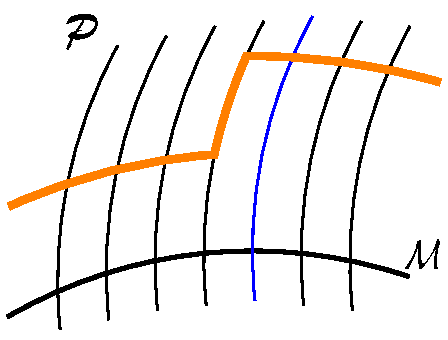
\includegraphics[width=.4\textwidth]{figures/Pbundle.pdf}
\caption{A schematic portrait of the space ${\cal P}_{h,n}$ as a fiber bundle over the moduli space ${\cal M}_{h,n}$. The (infinite dimensional) fiber over a given punctured Riemann surface $\Sigma\in {\cal M}_{h,n}$, indicated in blue, is parameterized by coefficients $f_{i,m}$ appearing in the transition maps (\ref{fimfom}) associated with the coordinate systems around each puncture on $\Sigma$. The integration contour $S_{h,n}$ that defines the off-shell amplitude (\ref{gamsecs}) is represented in orange.}\label{fig:Pbundle}
\end{figure}

Note that under a constant phase rotation of each $w_i$, or equivalently replacing $f_i(w_i) \to f_i(e^{i\A_i} w_i)$, $\Omega[\underline\Psi]$ is invariant due to the condition $L_0^-\Psi_i=0$ by definition of the string fields (\ref{blcon}). Furthermore, if $\delta f_i(w_i)$ represents the variation of $f_i(w_i)$ under an infinitesimal constant phase rotation of $w_i$, the corresponding variation of ${\cal B}$ does not affect $\Omega[\underline\Psi]$ due to the condition $b_0^-\Psi_i=0$ on the string fields. Consequently, $\Omega[\underline\Psi]$ induces a well-defined differential form on the quotient space
\ie
\widehat{\cal P}_{h,n} = {\cal P}_{h,n}/\{f_i(w_i) \sim f_i(e^{i\A_i} w_i), ~\forall \A_i\},
\fe
which is also a fiber bundle over ${\cal M}_{h,n}$. 

The string field amplitude, which can be interpreted as amputated off-shell Green function of string fields, is constructed as\footnote{Note that the normalization factor in (\ref{gamsecs}), which is standard in string field theory literature, differs from that of (\ref{omegaone}). This leads to a difference between the normalization of the string field and that of the vertex operator in Chapter \ref{chat:pertstring}, as well as a different normalization convention for the string coupling.}
\ie\label{gamsecs}
{\cal A}_{h,n}[\underline\Psi] = {1\over (-2\pi i )^{3h-3+n}} \int_{S_{h,n}} \Omega[\underline\Psi] ,
\fe
where $S_{h,n}$ is a $(6h-6+2n)$-dimensional cycle\footnote{i.e. an algebraic combination of integration contours.} that 

\noindent (i) is homologous to a section of the fiber bundle $\widehat{\cal P}_{h,n}\to{\cal M}_{h,n}$, 

\noindent (ii) is symmetric with respect to permutations on the $n$ punctures along with their associated holomorphic coordinate systems, and

\noindent (iii) satisfies a set of compatibility conditions of the form (\ref{limitgam}) near the boundary of ${\cal M}_{h,n}$, to be explained in section \ref{sec:sftonepi}.

Explicitly, integrating over $S_{h,n}$ is equivalent to setting each $f_{i,m}$ of (\ref{fimfom}) to be a chosen function of the moduli $t^k$, and then integrating the resulting differential form over ${\cal M}_{h,n}$. The off-shell amplitude generally depends on the choice of $S_{h,n}$. We will see in section \ref{sec:sftframe} this ambiguity is tied to the freedom in redefinition of the string field or equivalently the choice of a string field frame.



For Grassmann-even string fields $\Psi_i$, we define
\ie
Q_B \underline{\Psi} \equiv Q_B\Psi_1\otimes\Psi_2\otimes \cdots \otimes \Psi_n + \Psi_1\otimes Q_B\Psi_2\otimes \cdots \otimes \Psi_n + \cdots + \Psi_1\otimes\cdots\otimes Q_B \Psi_n,
\fe
and likewise with a minus sign included each time $Q_B$ moves past a Grassmann-odd string field. A key property of (\ref{omegathre}) is its BRST transformation (analogously to (\ref{omegapbrstvar}))
\ie\label{omegadom}
\Omega[Q_B\underline\Psi] &= \left\langle e^{\cal B} \,Q_B\cdot \prod_{i=1}^n [\Psi_i(0)]^{f_i} \right\rangle = \left\langle - (Q_B {\cal B})\, e^{\cal B} \prod_{i=1}^n [\Psi_i(0)]^{f_i} \right\rangle
\\
&=- \left(\sum_k dt^k \partial_{t^k} +\sum_{i=1}^n \sum_{m=0}^\infty df_{i,m} {\partial\over \partial f_{i,m}} \right) \left\langle e^{\cal B} \prod_{i=1}^n [\Psi_i(0)]^{f_i} \right\rangle = - d\Omega[\underline\Psi],
\fe 
where in the second line we have used Ward identities for the conformal transformations $f_i$. If we restrict the string fields $\Psi_i$ to be on-shell, namely $Q_B \Psi_i=0$, it then follows from (\ref{omegadom}) that $d\Omega[\underline\Psi]=0$, i.e. $\Omega[\underline\Psi]$ is a closed form in $\widehat{\cal P}_{h,n}$ and the dependence of (\ref{gamsecs}) on the cycle $S_{h,n}$ drops out modulo the aforementioned divergence near the boundary of the moduli space, recovering the prescription of Chapter \ref{chat:pertstring}.





\subsection{1PI effective action in Siegel gauge}
\label{sec:sftonepi}


The off-shell amplitude (\ref{gamsecs}) may be decomposed as tree Feynman diagrams consisting of 1PI amplitudes/vertices joined with string field propagators, as follows. Recall that the integration near the boundary of ${\cal M}_{h,n}$ (\ref{ampnearxxb}), where the Riemann surface $\Sigma$ pinches into a pair of surfaces $\Sigma_1$ and $\Sigma_2$ joined via (\ref{gluingmapzz}), gives rise to 1-particle poles in the on-shell string amplitude. The same consideration applies to the off-shell amplitude provided that in the degeneration limit $q\to 0$ the cycle $S_{h,n}$, viewed as an (averaged) section of $\widehat{\cal P}_{h,n}\to {\cal M}_{h,n}$, is related to the cycles $S_{g_1, n_1}$ and $S_{g_2, n_2}$ used to define the sub-amplitudes associated with the surfaces $\Sigma_1$ and $\Sigma_2$ by the compatibility condition
\ie\label{limitgam}
S_{h,n}\; \to ~ \widehat\varrho \left(\widetilde S_{g_1, n_1} \times \widetilde S_{g_2, n_2}\times \{q: |q| \ll 1\} \right),
\fe
where $\widetilde S_{g_i, n_i}$ is a lift of the cycle $S_{g_i, n_i}$ from $\widehat{\cal P}_{g_i,n_i}$ to (a chain in) ${\cal P}_{g_i,n_i}$, $\varrho$ is the plumbing map
\ie\label{varrhodef}
\varrho :~ {\cal P}_{g_1,n_1} \times {\cal P}_{g_2,n_2} \times \{q: |q|<1\} \to {\cal P}_{h,n}
\fe
induced from (\ref{gluingmapzz}), and $\widehat\varrho$ is $\varrho$ followed by the projection ${\cal P}_{h,n}\to \widehat{\cal P}_{h,n}$. That is, given the punctured surfaces $\Sigma_1, \Sigma_2$ with the choice of a holomorphic coordinate system around each puncture, we form the surface $\Sigma$ by sewing together a pair of punctures contained in the discs $D_1\subset\Sigma_1$ and $D_2\subset\Sigma_2$ as in (\ref{gluingmapzz}), keeping the data of the holomorphic coordinate systems around all of the remaining punctures (but omitting those on $D_1$ and $D_2$) which specifies the image of $\varrho$ in $\widehat P_{h,n}$. 

The analog of (\ref{ampnearxxb}) or (\ref{foupiss}) for the off-shell amplitude is
\ie\label{factoffsamp}
\sum_{\A,\B} {\cal A}_{g_1,n_1}[\Psi_1\otimes\cdots \otimes \Psi_{n_1-1}\otimes \phi_\A] \, \langle\langle \phi_\A^c | {b_0^+ b_0^- \over L_0^+} | \phi_\B^c \rangle \, {\cal A}_{g_2,n_2}[\phi_\B\otimes\Psi_{n_1}\otimes\cdots \otimes \Psi_n] ,
\fe
where we have assumed, without loss of generality, that $\Psi_1,\cdots,\Psi_{n_1-1}$ are inserted on $\Sigma_1$ whereas $\Psi_{n_1},\cdots,\Psi_{n=n_1+n_2-2}$ are inserted on $\Sigma_2$. Here $\phi_\A$ is a basis of ${\rm Ker}(b_0^+)\subset {\cal H}_0$, i.e. the space of string fields $\Psi$ that obey the Siegel gauge condition\footnote{The sense in which this is a gauge condition will be explained in classical string field theory in section \ref{sec:sfteom} and in the quantum string field theory in section \ref{bvsftsec}.}
\ie\label{siegelgauge}
b_0^+\Psi=0,
\fe
and $\phi_\A^c$ is a dual basis of $c_0 \widetilde c_0 {\cal H}_0 \subset {\cal H}_{\rm m}\otimes {\cal H}_{\rm gh}$ that satisfy the completeness relation
\ie\label{bzcz}
\sum_\A |\phi_\A\rangle \langle\langle \phi_\A^c|  = b_0^+ c_0^+,
\fe
where the RHS is equivalent to a projector onto ${\rm Ker}(b_0^+)$. (\ref{factoffsamp}) may be viewed as the Feynman diagram formed by joining the off-shell sub-amplitudes ${\cal A}_{g_1, n_1}$ and ${\cal A}_{g_2,n_2}$ with the propagator of a basis of string fields $\phi_\A$ in the Siegel gauge.

We can then express $\sum_{h=0}^\infty {\cal A}_{h,n}[\underline\Psi]$ as the sum over tree Feynman diagrams whose internal lines are those of string fields in the Siegel gauge, with the propagator
\ie
{b_0^+ b_0^-\over L_0^+},
\fe
and whose vertices are the 1PI amplitudes ${\cal A}_n^{\rm 1PI}$. The 1PI effective action $\Gamma[\Psi]$ in the Siegel gauge can be written as (in the Euclidean signature convention)
\ie\label{gamsieg}
\Gamma[\Psi] = {1\over 2} \langle\langle \Psi | c_0^- c_0^+ L_0^+ |\Psi\rangle - \sum_{n=1}^\infty {1\over n!} {\cal A}_n^{\rm 1PI}[\Psi^{\otimes n}].
\fe
Equivalently, $\Gamma[\Psi]$ can be obtained from the generating functional
\ie
W[\Psi] = \sum_{n=1}^\infty {1\over n!} \sum_{h=0}^\infty {\cal A}_{h,n}[\Psi^{\otimes n}],
\fe
where the sum excludes $h=0$, $n=1,2$ terms, 
by a Legendre transformation
\ie\label{offshellgamma}
\Gamma[\Phi] & =  -\left. \left[ W[\Psi] + {1\over 2} \langle\langle \Psi|  c_0^- c_0^+ L_0^+ |\Psi\rangle - \langle \langle \Phi|  c_0^- c_0^+ L_0^+|\Psi\rangle\right] \right|_{\rm stat.},
\fe
where the string fields $\Phi$, $\Psi$ are both assumed to obey the Siegel gauge condition (\ref{siegelgauge}), and the RHS of (\ref{offshellgamma}) is evaluated at the stationary point with respect to $\Psi$.


It is now possible to handle mass and field renormalization by re-calculating string scattering amplitudes using tree Feynman diagrams derived from the 1PI effective action $\Gamma[\Psi]$, normalizing the external fields according to the quantum-corrected kinetic term in $\Gamma[\Psi]$, and adjusting the external momenta according to the quantum-corrected position of the LSZ pole. Likewise, the quantum corrections to the vacuum configuration are handled by finding the stationary point of $\Gamma[\Psi]$ that may require turning on a nonzero string field $\Psi$, and re-formulating perturbation theory around this stationary point.



%In $c=1$ string theory, the effective string coupling vanishes in the asymptotic region and consequently we don't need to worry about mass and field renormalization. %On the other hand, these issues will be relevant in superstring and heterotic string theories, as we will discuss in section \ref{sec:supersft}.


\subsection{Classical string field theory}
\label{sec:sfteom}

It is instructive to inspect the classical limit of the effective action, where we keep only the genus zero contribution to the 1PI amplitudes ${\cal A}_n^{\rm 1PI}$. To begin with, the $(h,n)=(0,3)$ 1PI amplitude is the same as the sphere 3-point off-shell amplitude
\ie
{\cal A}_{0,3}[\Psi^{\otimes 3}] = \left\langle \prod_{i=1}^3 [\Psi(0)]^{f_i^{0,3}} \right\rangle,
\fe
where the (0-dimensional) cycle $S_{0,3}$ simply amounts to a choice of three conformal maps $f_1^{0,3}, f_2^{0,3}, f_3^{0,3}$ that are related to one another by the $PSL(2,\mathbb{C})$ automorphisms permuting the three punctures at $z_i=f_i(0)$. We will also refer to this cycle as the ``3-string vertex'' $\Gamma_{0,3}$. A possible explicit choice is\footnote{Note that $f_i$ need not be $PSL(2,\mathbb{C})$ maps in general. Examples of other choices will be considered in section \ref{sec:sftframe}.}
\ie\label{fpsltc}
f_1^{0,3}(w_1) = {w_1\over 3r}, ~~~~ f_2^{0,3}(w_2) = {1+{w_2\over 3r}\over 1- {w_2\over r}},~~~~ f_3^{0,3}(w_3) = {-1 + {w_3\over 3r}\over 1 + {w_3\over r}},
\fe
where $r$ is a nonzero constant, and the punctures are located at $z_1=0$, $z_2 = 1$, $z_3=-1$. For the purpose of plumbing fixture construction, we should demand that the discs $D_i = \{z=f_i^{0,3}(w_i): |w_i|<1\}$ do not overlap, which requires $r\geq 1$.

Next, consider the sphere 4-point off-shell amplitude
\ie
{\cal A}_{0,4}[\Psi^{\otimes 4}] =  \int_{\mathbb{C}}  {i dt \wedge d\bar t\over 2\pi} \left\langle {\cal B}_{\bar t} {\cal B}_t  \prod_{i=1}^4 [\Psi(0)]^{f_i^{0,4}} \right\rangle,
\fe
where we have re-expressed the integration over the cycle ${\cal S}_{0,4}$ as one over the moduli space ${\cal M}_{0,4}$ parameterized by the cross ratio $t = {z_{12}z_{34}\over z_{14}z_{32}}$, together with the choice of conformal maps $f_i^{0,4}$ with $f_i^{0,4}(0)=z_i$, $i=1,\cdots,4$. The compatibility condition is such that near the boundary of ${\cal M}_{0,4}$, namely the degeneration limits $t\to 0, 1$, or $\infty$ where the 4-punctured sphere $\Sigma_{0,4}$ is obtained by joining a pair of 3-punctured spheres via the plumbing fixture (\ref{gluingmapzz}) with $q\to 0$, the conformal maps $f_1^{0,4},\cdots, f_4^{0,4}$ should agree with the local holomorphic coordinate maps associated with the unsewed punctures. In particular, this condition can be satisfied if we simply demand that ${\cal S}_{0,4}$, as a section of $\pi:\hat{\cal P}_{0,4}\to {\cal M}_{0,4}$, agrees with $\widehat\varrho (\widetilde\Gamma_{0,3}\times \widetilde\Gamma_{0,3}\times \{q:|q|<1\})$ (in the notation of (\ref{limitgam})) whenever $\Sigma_{0,4}$ is obtained by the plumbing fixture. More explicitly, we can divide ${\cal M}_{0,4}$ into four domains,
\ie
{\cal M}_{0,4} = \cD_s \cup \cD_t \cup \cD_u \cup \cD_{0,4},
\fe
where $\cD_s$ consists of $\Sigma_{0,4}$ obtained by sewing a pair of spheres, with the punctures $1, 2$ on the first sphere and $3,4$ on the second sphere,\footnote{In the case where the 3-string vertex $\Gamma_{0,3}$ is constructed using the $PSL(2,\mathbb{C})$ conformal maps (\ref{fpsltc}), we can express $\cD_s$ as
\ie
\cD_s &= \bigg\{ t = {z_{12}z_{34}\over z_{14}z_{32}}: z_1 = f_1^{0,3}(0),~z_2 = f_2^{0,3}(0),
\\
&~~~~z_3 = f_3^{0,3} \Big({q\over (f_1^{0,3})^{-1}\circ f_2^{0,3}(0)}\Big), ~z_4 = f_3^{0,3} \Big({q\over (f_1^{0,3})^{-1}\circ f_3^{0,3}(0)}\Big), ~|q|<1 \bigg\},
\fe
where $(f_1^{0,3})^{-1}\circ f_2^{0,3}$ is defined by the analytic continuation of $(f_1^{0,3})^{-1}$ from $\{f_1^{0,3}(w):|w|<1\}$ (which does not contain the point $f_2^{0,3}(0)$) to the rest of the complex plane.} $\cD_t$ and $\cD_u$ are related to $\cD_s$ by swapping $1\leftrightarrow 3$ and $1\leftrightarrow 4$, and $\cD_{0,4}={\cal M}_{0,4}\backslash (\cD_s \cup \cD_t \cup \cD_u)$ consists of $\Sigma_{0,4}$ that cannot be obtained by the plumbing fixture construction. The contribution from the segments of ${\cal S}_{0,4}$ over $\cD_s, \cD_t, \cD_u$ are precisely the sum of three tree-level Feynman diagrams built out of the 3-string vertex, where the internal string field is restricted to the Siegel gauge. The remaining segment of ${\cal S}_{0,4}$ over $\cD_{0,4}$, which we refer to as the 4-string vertex $\Gamma_{0,4}$, gives the 1PI amplitude
\ie\label{azerof}
{\cal A}_{0,4}^{\rm 1PI} [\Psi^{\otimes 4}] =  \int_{\cD_{0,4}}  {i dt \wedge d\bar t\over 2\pi} \left\langle {\cal B}_{\bar t} {\cal B}_t  \prod_{i=1}^4 [\Psi(0)]^{f_i^{0,4}} \right\rangle.
\fe
Continuity of the section ${\cal S}_{0,4}$ demands that $f_i^{0,4}(w_i)$ depends continuously on the moduli $(t, \bar t)$ within the domain ${\cal D}_{0,4}$, and must agree over the boundary $\partial{\cal D}_{0,4}$, up to a (possibly $(t,\bar t)$-dependent) phase rotation of $w_i$, with the coordinate maps inherited from the plumbing fixture construction. This is equivalent to saying that the boundary of $\Gamma_{0,4}$ is formed out of a pair of $\Gamma_{0,3}$ according to
\ie
-\partial\Gamma_{0,4} = \widehat\varrho_{12,34}\left(\widetilde\Gamma_{0,3}\times \widetilde\Gamma_{0,3}\times \{q:|q|=1\}\right) + (1\leftrightarrow 3)+(1\leftrightarrow 4),
\fe
where the subscript ``${12,34}$'' on $\widehat\varrho$ in the first term on the RHS indicates the distribution of punctures in the $s$-channel: 1,2 on one of the spheres and 3,4 on the other, in the plumbing fixture construction; the second and third term correspond to the distributions of punctures in $t$ and $u$ respectively. The addition on the RHS is defined in the sense of chains, and the minus sign on the RHS accounts for the orientation of $\partial \Gamma_{0,4}$.

The above construction of $\Gamma_{0,4}$ can be extended inductively to that of the $n$-string vertex $\Gamma_{0,n}$ for all $n\geq 4$, whose projection $\pi(\Gamma_{0,n}) \equiv {\cal D}_{0,n} \subset {\cal M}_{0,n}$ is the domain of $n$-punctured spheres that cannot be obtained by plumbing, such that the coordinate maps $f_i^{0,n}$ over $\partial {\cal D}_{0,n}$, modulo phase redefinitions of the local coordinates, agree with those inherited from plumbing. The latter compatibility condition is equivalently expressed as
\ie\label{gamsphglu}
- \partial \Gamma_{0,n} = {1\over 2} \sum_{\A\sqcup\B = \{1,\cdots,n\}} \widehat\varrho_{\A,\B} \left( \widetilde\Gamma_{0,|\A|+1}\times \widetilde\Gamma_{0,|\B|+1}\times \{q:|q|=1\} \right),
\fe
where the sum is taken over all partitions of $\{1,\cdots, n\}$ into a pair of subsets $\A$ and $\B$ that consist of at least two elements each, and $|\A|$ denotes the number of elements of $\A$. $\widehat\varrho_{\A,\B}$ is defined by the plumbing fixture with the punctures labeled by $\A$ distributed on one of the spheres and those labeled by $\B$ on the other sphere. 

Generalizing (\ref{azerof}), the sphere $n$-point 1PI amplitude ${\cal A}_{0,n}^{\rm 1PI}$ is given by (\ref{gamsecs}) with the cycle $S_{0,n}$ replaced by the chain $\Gamma_{0,n}$. The genus zero part of the effective action (\ref{gamsieg}), which may be viewed as the action of classical string field theory in Siegel gauge, is
\ie\label{classsieg}
\left.S[\Psi]\right|_{b_0^+\Psi=0} = {1\over 2} \langle\langle \Psi | c_0^- c_0^+ L_0^+ |\Psi\rangle - \sum_{n=3}^\infty {1\over n!} {\cal A}_{0,n}^{\rm 1PI}[\Psi^{\otimes n}].
\fe
The linearized equation of motion derived by extremizing the kinetic term of (\ref{classsieg}) is $L_0^+\Psi=0$. While this is satisfied for a $Q_B$-closed string field $\Psi$ that obeys the Siegel gauge condition (\ref{siegelgauge}), it may appear unsatisfactory that the space of solutions to the linearized equation isn't quite the same as the BRST cohomology. Indeed, (\ref{classsieg}) can be viewed as a gauge-fixed version of the action
\ie\label{classicalsftact}
S[\Psi] = {1\over 2} \langle\langle \Psi | c_0^- Q_B |\Psi\rangle + \sum_{n=3}^\infty {1\over n!} \{\Psi^{\otimes n} \}_{0,n},
\fe
where we have defined the genus zero, $n$-string vertex $\{\underline\Psi \}_{0,n}$ as $-{\cal A}_{0,n}^{\rm 1PI}[\underline\Psi]$, i.e.
\ie\label{strvertgenzer}
\{ \Psi_1\otimes\cdots\otimes \Psi_n \}_{0,n} = - {1\over (-2\pi i )^{3h-3+n}} \int_{\Gamma_{0,n}} \Omega[\underline\Psi] ,
\fe
now without the restriction (\ref{siegelgauge}). Using the fact that $b_0^+c_0^+$ (\ref{bzcz}) is a projector onto ${\rm Ker} b_0^+$, and the identity $c_0^- Q_B b_0^+ c_0^+ = c_0^-c_0^+ L_0^+ + b_0^+ c_0^- Q_B c_0^+$, we see that (\ref{classicalsftact}) reduces to (\ref{classsieg}) upon imposing $b_0^+\Psi=0$. 

The equation of motion that follows from extremizing the action (\ref{classicalsftact}) takes the form
\ie\label{clsfteom}
E[\Psi]\equiv Q_B \Psi + \sum_{n=2}^\infty {1\over n!}  [\Psi^{\otimes n} ] = 0,
\fe
where the {\it string bracket} $[\Psi^{\otimes n} ]$ is a graded-symmetric $n$-linear map ${\cal H}_0^{\otimes n}\to {\cal H}_0$ defined in terms of the $(n+1)$-string vertex via the property
\ie\label{stringbradefpro}
\langle\langle \Phi|c_0^- |  [\Psi^{\otimes n} ] \rangle =  \{ \Phi\otimes \Psi^{\otimes n}  \}_{0,n+1},~~~~\forall \,\Phi\in {\cal H}_0.
\fe
To see that (\ref{stringbradefpro}) defines $[\Psi^{\otimes n} ]$ unambiguously, it suffices to show that it determines $\langle\chi|  [\Psi^{\otimes n} ]\rangle$ for any spinless $\chi \in {\cal H}_{\rm m}\otimes {\cal H}_{\rm gh}$, i.e. $\chi$ is annihilated by $L_0^-$ but not necessarily by $b_0^-$. By assumption $[\Psi^{\otimes n} ]$ is annihilated by $b_0^-$, and so we can write
\ie\label{umabistrbr}
\langle\chi|  [\Psi^{\otimes n} ]\rangle &= \langle\chi| (b_0^-c_0^- + c_0^- b_0^-)|  [\Psi^{\otimes n} ]\rangle
= \langle\chi| b_0^- c_0^-|  [\Psi^{\otimes n} ]\rangle 
= (-)^{|\chi|}  \{ b_0^-\chi \otimes \Psi^{\otimes n}  \}_{0,n+1},
\fe
where $|\chi|$ stands for the Grassmann parity of $\chi$, thereby justifying the claim. Note that for a Grassmann-even string field $\Psi$, $[\Psi^{\otimes n} ]$ is Grassmann-odd. To obtain (\ref{clsfteom}) by variation of (\ref{classicalsftact}), we also need a subtle identity\footnote{Note that $Q_B$ does {\it not} commute with $c_0^-$. But, we have 
\ie
\langle\Phi|Q_B c_0^- |\Psi\rangle &= \langle\Phi|(b_0^-c_0^- + c_0^- b_0^-) Q_B c_0^- |\Psi\rangle = \langle\Phi| c_0^- b_0^- Q_B c_0^- |\Psi\rangle 
\\
&= \langle\Phi| c_0^- (L_0^- - Q_B b_0^-) c_0^- |\Psi\rangle = - \langle\Phi| c_0^- Q_B b_0^- c_0^- |\Psi\rangle = - \langle\Phi| c_0^- Q_B |\Psi\rangle.
\fe}
\ie\label{subtleid}
\langle \Phi | Q_B c_0^- |\Psi\rangle = - \langle \Phi| c_0^- Q_B |\Psi\rangle, ~~~~\forall \, \Phi,\Psi\in {\cal H}_0.
\fe


The {\it generalized BRST operator} $Q_\Psi$ is defined by
\ie\label{genbrstga}
Q_\Psi \Lambda \equiv Q_B \Lambda +  \sum_{n=1}^\infty {1\over n!}  [ \Lambda \otimes \Psi^{\otimes n}  ] ,
\fe
for any string field $\Lambda$. An essential property of the LHS of (\ref{clsfteom}) is that
\ie\label{qepsicpt}
Q_\Psi E[\Psi] = 0
\fe
holds for any string field $\Psi$, not necessarily obeying the equation of motion. (\ref{qepsicpt}) is a consequence of the following identity for the string brackets 
\ie\label{linfty}
Q_B  [ \Psi^{\otimes n}  ] + n  [ Q_B \Psi \otimes \Psi^{\otimes (n-1)} ]
+ \sum_{m=2}^{n-1} {n\choose m}  \big[  [ \Psi^{\otimes m} ] \otimes \Psi^{\otimes (n-m)}  \big] = 0,~~~~n\geq 2.
\fe
$Q_B$ together with the string brackets satisfying the relation (\ref{linfty}) define what is known as an $L_\infty$ algebra structure on the space of closed string fields. The proof of (\ref{linfty}), which follows from (\ref{gamsphglu}) and (\ref{omegadom}), will be deferred to section \ref{bvsftsec}, via the classical BV master equation satisfied by the action (\ref{classicalsftact}).


Importantly, the action $S[\Psi]$ (\ref{classicalsftact}) is invariant under the infinitesimal variation of the string field $\Psi$ by
\ie\label{gaugeclsft}
\delta_\Lambda \Psi = Q_\Psi\Lambda
\fe
for an arbitrary string field $\Lambda$, as\footnote{One can also see directly that the equation of motion (\ref{clsfteom}) is preserved, as $E[\Psi]$ varies  under (\ref{gaugeclsft}) by $\delta E[\Psi] = [\Lambda\otimes E[\Psi]\otimes e^{\otimes \Psi}]$. }
\ie
\delta_\Lambda S &= \langle\langle Q_\Psi\Lambda| c_0^- |E[\Psi]\rangle
= \langle\langle Q_B\Lambda| c_0^- |E[\Psi]\rangle + \sum_{n=1}^\infty {1\over n!} \langle\langle  [\Lambda\otimes \Psi^{\otimes n} ] |c_0^-| E[\Psi]\rangle
\\
&= \langle\langle \Lambda| c_0^- Q_B |E[\Psi]\rangle + \sum_{n=1}^\infty {1\over n!} \{ \Lambda\otimes \Psi^{\otimes n} \otimes E[\Psi] \} = \langle\langle\Lambda|c_0^- |Q_\Psi E[\Psi] \rangle = 0,
\fe
where in getting to the second line we used (\ref{subtleid}) and the symmetry of the string vertices, and the last equality follows from (\ref{qepsicpt}). At the linearized level, the transformation (\ref{gaugeclsft}) reduces to $\delta_\Lambda\Psi=Q_B \Lambda$, representing a trivial string state. This suggests that (\ref{gaugeclsft}) should be interpreted as a gauge redundancy of the full classical string field theory, and explains the sense in which the Siegel condition (\ref{siegelgauge}) is a choice of gauge.

Given a pair of (Grassmann-odd) string fields $\Lambda_1, \Lambda_2$, the commutator between the infinitesimal gauge transformations $\delta_{\Lambda_1}$ and $\delta_{\Lambda_2}$ acts by
\ie
(\delta_{\Lambda_1}\delta_{\Lambda_2}-\delta_{\Lambda_2}\delta_{\Lambda_1})\Psi = Q_\Psi [\Lambda_1\otimes \Lambda_2 \otimes e^{\otimes \Psi}] + \big[\Lambda_1\otimes \Lambda_2\otimes E[\Psi]\otimes e^{\otimes \Psi} \big],
\fe
where we have used the notation $e^{\otimes \Psi}\equiv \sum_{n=0}^\infty {1\over n!} \Psi^{\otimes n}$. We see that if $\Psi$ satisfies the equation of motion (\ref{clsfteom}), the commutator between the two gauge transformations is another gauge transformation generated by the string field 
\ie\label{gaugealgsft}
[\Lambda_1, \Lambda_2]_\Psi \equiv \big[ \Lambda_1\otimes \Lambda_2 \otimes e^{\otimes \Psi} \big].
\fe
In other words, the gauge algebra only closes ``on-shell'', and the gauge algebra structure ``constants'' depend explicitly on the field $\Psi$. These features are tied to the underlying $L_\infty$ algebra structure of the classical string field theory.






\subsection{Batalin-Vilkovisky formalism}
\label{sec:bvform}


The Batalin-Vilkovisky (BV) formulation of a quantum gauge theory is based on an auxiliary field space that consists of ordinary fields paired with ``anti-fields'', an action functional subject to consistency conditions known as the master equation, and the path integral defined over a Lagrangian field subspace whose choice amounts to a gauge condition. The BV formalism encompasses and generalizes the BRST formalism in a way that allows for consistent quantization when the gauge algebra structure is field dependent and only closes on-shell (as in (\ref{gaugealgsft})), and moreover provides a natural framework for Wilsonian effective gauge theory.

The BV field space is coordinatized by fields $\Phi^I$, which may be either Grassmann-even or odd, and corresponding anti-fields $\Phi_I^\ddagger$ with opposite Grassmann parity, paired through the Grassmann-odd symplectic form 
\ie
\omega = \delta\Phi_I^\ddagger \wedge \delta \Phi^I.
\fe
The BV anti-bracket between a pair of functionals ${\cal F}$ and ${\cal G}$ is defined as the Poisson bracket 
\ie\label{bvantibrack}
({\cal F},{\cal G}) \equiv {\delta_R {\cal F}\over\delta \Phi^I} {\delta {\cal G}\over \delta \Phi_I^\ddagger} - {\delta_R {\cal F}\over\delta \Phi_I^\ddagger} {\delta {\cal G}\over \delta \Phi^I},
\fe
where the differentiation $\delta/\delta\psi$ acts by stripping off $\psi$ from the left, whereas $\delta_R/\delta\psi$ acts by stripping off $\psi$ from the right, which may differ by a sign due to the presence of Grassmann-odd variables.

The BV gauge condition amounts to a choice of a Lagrangian field-subspace, of the form\footnote{A Lagrangian subspace $L$ is a half-dimensional subspace on which the symplectic form $\omega$ vanishes. Assuming that $\Phi^I$ are non-degenerate coordinates, $L$ takes the form $L_V$ (\ref{bvfix}) as $\omega|_{L_V} = {\delta_R \delta V\over \delta\Phi^J\delta \Phi^I} \delta\Phi^J \wedge \delta\Phi^I$=0.}
\ie\label{bvfix}
L_V: ~ \Phi_I^\ddagger = {\delta V[\Phi]\over \delta \Phi^I},
\fe
where $V[\Phi]$ is a Grassmann-odd functional. The path integral is formulated as a functional integral over (\ref{bvfix}) with an action functional $S[\Phi,\Phi^\ddagger]$, of the form
\ie\label{gaugefixedbvpath}
Z_V = \int_{L_V} d\Phi\, e^{- S[\Phi,\Phi^\ddagger]} = \int d\Phi \, e^{-S_V[\Phi]},~~~~ S_V[\Phi] \equiv S\left[\Phi, \Phi^\ddagger = {\delta V\over \delta\Phi}\right].
\fe
The idea is that physical observables should be independent of the gauge condition $L_V$. To see when this is satisfied, let us consider an infinitesimal variation of the gauge condition by
\ie\label{bvgaugevar}
V[\Phi] \to V[\Phi] + \delta' V[\Phi],
\fe
under which the path integral (\ref{gaugefixedbvpath}) changes by
\ie\label{zvvars}
\delta' Z_V & = \int_{L_V} d\Phi \, {\delta_R \over \delta\Phi_I^\ddagger} e^{-S[\Phi,\Phi^\ddagger] }\,  {\delta (\delta'V[\Phi])\over \delta\Phi^I}
\\
& = - \int_{L_V} d\Phi\, \left(  {\delta_R \over \delta\Phi_I^\ddagger}{\delta\over \delta\Phi^I} e^{-S[\Phi,\Phi^\ddagger]} + {\delta^2 V\over \delta\Phi^I \delta \Phi^J} \, {\delta_R \over \delta\Phi_I^\ddagger}{\delta\over \delta\Phi_J^\ddagger} e^{-S[\Phi,\Phi^\ddagger]} \right) \delta'V[\Phi],
\fe
where in getting to the second line we have integrated by part with respect to $\Phi^I$. The opposite Grassmann parity of the fields and anti-fields is such that ${\delta^2 V\over \delta\Phi^I \delta \Phi^J} \, {\delta_R \over \delta\Phi_I^\ddagger}{\delta\over \delta\Phi_J^\ddagger} e^{-S} \equiv 0$, and thus the RHS of (\ref{zvvars}) vanishes provided
\ie\label{qbvmastabs}
{\delta_R \over \delta\Phi_I^\ddagger}{\delta\over \delta\Phi^I} e^{-S[\Phi,\Phi^\ddagger]} = 0.
\fe
The condition (\ref{qbvmastabs}) is known as the {\it quantum BV master equation}. In terms of the BV anti-bracket (\ref{bvantibrack}) and $\Delta_\Phi \equiv {\delta_R\over \delta\Phi_I^\ddagger}{\delta_L\over \delta\Phi^I}$, (\ref{qbvmastabs}) can be equivalently written as
\ie\label{ssbvmast}
({S}, {S}) + 2 \Delta_\Phi{{S}} = 0.
\fe
Similarly, the expectation value of ${\cal O}[\Phi]$ changes under (\ref{bvgaugevar}) by (assuming $S$ satisfies the quantum master equation \ref{ssbvmast})
\ie
\delta' \big\langle{\cal O}\big\rangle_V & = \int_{L_V} d\Phi \, {\delta_R \over \delta\Phi_I^\ddagger} e^{-S[\Phi,\Phi^\ddagger] }\, {\cal O}[\Phi]   {\delta (\delta'V[\Phi])\over \delta\Phi^I} 
\\
&= \int_{L_V} d\Phi\, e^{-S[\Phi,\Phi^\ddagger] }  {\delta_R S\over \delta\Phi_I^\ddagger}  {\delta {\cal O}\over \delta\Phi^I} \,\delta'V[\Phi] = -\big\langle (S, {\cal O}) \,\delta'V[\Phi] \big\rangle_V,
\fe
which vanishes provided $(S, {\cal O})=0$. The latter is the condition for ${\cal O}[\Phi]$ to define a physical observable, generalizing the notion of physicality in the BRST formalism.



\subsection{The BV formulation of quantum string field theory}
\label{bvsftsec}

Using recipes similar to those of section \ref{sec:sfteom} but extended to higher genera, it is possible to construct a BV action functional for the closed string field that satisfies the quantum BV master equation, thereby defining the quantum closed string field theory at least at the perturbative level through what amounts to a Wilsonian path integral.

To begin with, the full space of string fields ${\cal H}_0$ (\ref{blcon}) is equipped with the symplectic structure of the BV field space, as follows. We can split 
\ie
{\cal H}_0 = {\cal H}_0^- \oplus {\cal H}_0^+,
\fe
where ${\cal H}_0^-$ is the subspace spanned by states of total (left and right) ghost number $\leq 2$, and ${\cal H}_0^+$ is spanned by states of ghost number $\geq 3$. Let $|\phi_I\rangle$ be a basis for ${\cal H}_0^-$, and $|\phi^{I\ddagger}\rangle$ a dual basis for ${\cal H}_0^+$ that satisfy\footnote{Note that the BPZ conjugate $\langle\langle \cdot|$ is such that $\langle\langle \phi| c_0^- = (-)^{|\phi|+1} \langle\langle c_0^- \phi|$, where $|\phi|$ is the Grassmann parity of $\phi$.}
\ie\label{basisinnnersft}
& \langle\langle \phi^{I\ddagger}|c_0^-| \phi_J\rangle = \delta^I_J, ~~~~\langle\langle \phi_I| c_0^- |\phi^{J\ddagger}\rangle =  \delta_I^J,
\\
& \sum_I |\phi_I\rangle \langle\langle \phi^{I\ddagger}| c_0^- = 1_{{\cal H}_0^-},~~~~ \sum_I |\phi^{I\ddagger}\rangle \langle\langle \phi_I| c_0^- =  1_{{\cal H}_0^+}.
\fe
A general string field $\Psi$ can be expanded as
\ie
|\Psi\rangle = \sum_I  |\phi_I\rangle \psi^I - \sum_I \psi_I^\ddagger |\phi^{I\ddagger}\rangle,
\fe
where the coefficient field variables $\psi^I$ and $\psi_I^\ddagger$ have opposite Grassmann parity. We will view $\psi^I$ as the ordinary fields and $\psi_I^\ddagger$ as the anti-fields, paired through the symplectic form 
\ie\label{sftsympform}
\omega = \sum_I d\psi_I^\ddagger \wedge d\psi^I.
\fe
The BV action functional $S[\Psi]$ will take the form
\ie\label{bvsftfnl}
S[\Psi] = {1\over 2} \langle\langle\Psi|c_0^- Q_B|\Psi\rangle +  \sum_{n=1}^\infty \sum_{h=0}^\infty {1\over n!} \{\Psi^{\otimes n}\}_{h,n},
\fe
where the genus $h$, $n$-string vertex $\{\cdot \}_{h,n}:{\cal H}_0^{\otimes n}\to \mathbb{C}$ is a graded symmetric $n$-linear function, constructed as
\ie\label{psibracketg}
\{\Psi^{\otimes n}\}_{h,n} = - {1\over (-2\pi i)^{3h-3+n}} \int_{\Gamma_{h,n}} \Omega[\Psi^{\otimes n}],
\fe
for $h=0, n\geq 3$ and $h\geq 1, n\geq 1$, generalizing (\ref{strvertgenzer}), and is defined to trivially vanish for $h=0, n=1,2$. The differential form $\Omega[\underline\Psi]$ is constructed as in (\ref{omegathre}). $\Gamma_{h,n}$ is a $(6h-6+2n)$-dimensional chain in $\widehat{\cal P}_{h,n}$ that is symmetric with respect to permutations on the $n$ punctures (along with their associated holomorphic coordinate systems), subject to the following compatibility conditions that generalize (\ref{gamsphglu}),
\ie\label{stringvcomp}
- \partial \Gamma_{h,n} &= {1\over 2} \sum_{g_1+g_2=h} \sum_{\A\sqcup\B = \{1,\cdots,n\}} \widehat\varrho_{\A,\B} \left( \widetilde\Gamma_{g_1,|\A|+1}\times \widetilde\Gamma_{g_2,|\B|+1}\times \{q:|q|=1\} \right)
\\
&~~~ +  \widehat\varrho \left(\widetilde \Gamma_{h-1, n+2}\times \{q: |q|=1\}\right),
\fe
where $\widehat\varrho_{\A,\B}$ is defined by sewing the pair of surfaces $\Sigma_1$ and $\Sigma_2$ through the plumbing fixture as in (\ref{limitgam}), (\ref{varrhodef}), where the punctures labeled by $\A$ are distributed on $\Sigma_1$, and those labeled by $\B$ on $\Sigma_2$. $\widehat\varrho$ in the second line of (\ref{stringvcomp}) is defined by an analogous plumbing fixture construction that sews together the first pair of punctures on a single Riemann surface, which increases genus by one and reduce the total number of punctures by 2.

The quantum BV master equation (\ref{ssbvmast}) for the action (\ref{bvsftfnl}), expanded in genus and powers of the string field, reads
\ie\label{sftbveq}
& n \{ Q_B \Psi \otimes \Psi^{n-1} \}_{h, n} + \sum_{g_1+g_2=h} \sum_{n_1+n_2=n} {n!\over n_1! n_2!} \sum_I \{ \Psi^{\otimes n_1} \otimes \phi^{I\ddagger} \}_{g_1,n_1+1} \{ \phi_I \otimes \Psi^{\otimes n_2}\}_{g_2,n_2+1} 
\\
& +  \sum_I \{ \phi_I\otimes \phi^{I\ddagger} \otimes \Psi^{\otimes n}  \}_{h-1,n+2} = 0,
\fe
for $h=0, n\geq 3$ and $h\geq 1, n\geq 0$. The first term on the LHS of (\ref{sftbveq}) can be rewritten using (\ref{omegadom}) as
\ie\label{sftbvmaster}
\{ Q_B \Psi^{\otimes n} \}_{h,n} = - {1\over (-2\pi i)^{3h-3+n}} \int_{\Gamma_{h,n}} \Omega [Q_B \Psi^{\otimes n}] = {1\over (-2\pi i)^{3h-3+n}}\int_{\partial\Gamma_{h,n}} \Omega[\Psi^{\otimes n}] .
\fe
The second term on the LHS of (\ref{sftbveq}) can be simplified using the plumbing relation
\ie{}
& \left. \Omega[\Psi^{\otimes n}] \right|_{\varrho \left(\widetilde\Gamma_{g_1, n_1+1}\times \widetilde\Gamma_{g_2, n_2+1}\times \{q = e^{2\pi i \tau_1} \}\right)} 
\\
& = \sum_I \left\langle e^{\cal B} \prod_{i=1}^{n_1} [\Psi(0)]^{f_i}\big[ d\tau_1 {\cal B}_{\tau_1} c_0^- \phi^{I\ddagger}(0)\big]^{f_{n_1+1}} \right\rangle_{\Sigma_1} \left\langle [\phi_I(0)]^{f_{n_2+1}} e^{\cal B} \prod_{j=1}^{n_2} [\Psi(0)]^{f_j'}  \right\rangle_{\Sigma_2} + (\phi^{I\ddagger}\leftrightarrow \phi_I),
\fe
where $\{f_i\}_{i=1}^{n_1+1}$ ($\{f_j'\}_{j=1}^{n_2+1}$) are the conformal maps that define the coordinate systems around the punctures on $\Sigma_1$ ($\Sigma_2$), and ${\cal B}_{\tau_1}=2\pi i b_0^-$ is the $b$ ghost insertion associated with the modulus $\tau_1$, leading to
\ie\label{omegsew}
& {1\over (-2\pi i)^{3h-3+n}} \int_{\widehat\varrho \left(\widetilde\Gamma_{g_1, n_1+1}\times \widetilde\Gamma_{g_2, n_2+1}\times \{q:|q|=1\}\right) } \Omega[\Psi^{\otimes n}]
\\
&=\sum_I  \{ \Psi^{\otimes n_1} \otimes \phi^{I\ddagger} \}_{g_1,n_1+1} \{ \phi_I \otimes \Psi^{\otimes n_2}\}_{g_2,n_2+1} + (\phi^{I\ddagger}\leftrightarrow \phi_I).
\fe
Similarly, the third term on the LHS of (\ref{sftbveq}) can be rewritten via self-plumbing as
\ie\label{omgselfsew}
\sum_I \{ \phi_I\otimes \phi^{I\ddagger} \otimes \Psi^{\otimes n}  \}_{h-1,n+2} = {1\over 2 (-2\pi i)^{3h-3+n} } \int_{\widehat\varrho \left(\widetilde \Gamma_{h-1, n+2}\times \{q: |q|=1\}\right)} \Omega[\Psi^{\otimes n}].
\fe
Putting these relations together, one finds that the quantum master equation (\ref{sftbveq}) follows from the compatibility condition (\ref{stringvcomp}) (also known as the ``geometric master equation'').

The BV action (\ref{bvsftfnl}) with the string vertices defined by $\Gamma_{h,n}$ satisfying (\ref{stringvcomp}) therefore defines a consistent quantum closed string field theory, at least perturbatively in the string fields. To formulate the string field path integral, one should impose a BV gauge condition that amounts to choosing a Lagrangian subspace of ${\cal H}_0$ with respect to the symplectic form (\ref{sftsympform}). An example is the Siegel gauge condition $b_0^+\Psi=0$ as we have already encountered. In the classical limit, the BV action retains only the $h=0$ terms in (\ref{bvsftfnl}) and reduces to the classical string field theory action (\ref{classicalsftact}). The classical limit of the BV master equation (\ref{ssbvmast}) is 
\ie\label{clasbvmast}
(S,S)=0, 
\fe
which is equivalent to (\ref{qepsicpt}) or the $L_\infty$ relation (\ref{linfty}).





\subsection{String vertices and field redefinition}
\label{sec:sftframe}

In the classical string field theory (section \ref{sec:sfteom}), a consistent set of string vertices or equivalently the chains $\Gamma_{0,n}$ that obey the geometric master equation (\ref{gamsphglu}) may be constructed simply using $PSL(2,\mathbb{C})$ coordinate maps $f_i^{0,n}$. 

An alternative set of string vertices can be constructed using the minimal area Hermitian metric on $\Sigma' =\Sigma \backslash \sqcup_i D_i$, where $D_i$ is the unit disc in the local coordinate system around the $i$-th puncture, subject to the constraint that every non-contractible closed curve has length $\geq 2\pi$. Note that the strict convexity of the area functional with respect to the metric implies that the minimal area metric is unique. For genus zero surface $\Sigma$, the minimal area metric on $\Sigma'$ is foliated by bands of geodesics of length $2\pi$, and is flat everywhere except where different geodesic bands meet.\footnote{Note that on a higher genus surface, the geodesic bands may cross and the minimal area metric is not almost everywhere flat.} The string vertices $\Gamma_{0,n}$ may be defined by the coordinate maps associated with the minimal area metrics on $\Sigma'$, over the moduli domain $\pi(\Gamma_{0,n})\subset {\cal M}_{0,n}$ where the internal geodesic bands have height $\leq 2\ell$, and that all external geodesic bands (``stubs'') that meet $\partial D_i$ have height $\ell$, for some $\ell\geq 0$. 

The ``most efficient'' minimal area vertices for the classical string field theory, where the domains $\pi(\Gamma_{0,n})$ for $n\geq 4$ are minimized, are given by the choice $\ell=0$. In this case, the area of the metric on $\Sigma'$ vanishes. Note however that the moduli domain $\pi(\Gamma_{0,n})$ still has nonzero measure. For instance, $\Sigma'$ in $\Gamma_{0,4}$ may be constructed as a tetrahedron skeleton whose three pairs of opposing edges have length $t_1, t_2, t_3$, such that $t_i\leq \pi$ and $t_1+t_2+t_3=2\pi$.

For the quantum string field theory, a consistent set of string vertices $\Gamma_{h,n}$ for all genera $h$ can be constructed using the hyperbolic Hermitian metric on $\Sigma'$ of Gaussian curvature $-1$ (or equivalently, Ricci scalar $R=-2$), such that every boundary component $\partial D_i$ is a geodesic of length $L$, and that all closed geodesics have length $\geq L$. It can be shown that such $\Gamma_{h,n}$'s solve the geometric master equation provided\footnote{Costello and Zwiebach, JHEP \textbf{02} (2022), 2 \cite{Costello:2019fuh}.} 
\ie\label{lstarc}
L\leq L_* = 2 \, {\rm arcsinh} (1) \approx 1.76275.
\fe

A deformation of the set of string vertices, $\Gamma_{h,n}\to \Gamma_{h,n}'$, subject to the consistency condition imposed by the geometric master equation, a priori deforms the string field action functional, $S[\Psi]\to S'[\Psi]$. It will turn out that $S'$ and $S$ in fact define string field theories that are related by field redefinitions, and are equivalent at the level of physical observables. To understand this, we begin by noting that the change of the SFT action $S[\Psi]$ under an infinitesimal deformation of consistent string vertices can be written in the form
\ie\label{salphadef}
\overline\delta S = (S, \A) + \Delta\A,
\fe
where the BV anti-bracket $(\cdot,\cdot)$ and $\Delta$ are defined as in the quantum master equation (\ref{ssbvmast}), and $\A$ is a functional of the string field $\Psi$. Explicitly, suppose the infinitesimal change of string vertex $\Gamma_{h,n}$ is associated with the deformation of coordinate maps $f_i \to f_i + \overline\delta f_i$, the functional $\A$ is constructed as
\ie\label{alphapsi}
\A[\Psi] &= - \sum_{n=1}^\infty \sum_{h=0}^\infty {1\over n! (-2\pi i)^{3h-3+n}}\int_{\Gamma_{h,n}} \sum_{i=1}^n\sum_{m=0}^\infty \overline\delta f_{i,m} \iota_{\partial\over \partial f_{i,m}} \Omega_{6h-5+2n}[\Psi^{\otimes n}]
\\
&= - \sum_{n=1}^\infty \sum_{h=0}^\infty {1\over n! (-2\pi i)^{3h-3+n}}\int_{\Gamma_{h,n}} \left\langle {\cal B}_{\overline\delta}\, e^{\cal B} \prod_{i=1}^n [\Psi(0)]^{f_i} \right\rangle,
\fe
where the notations are as in (\ref{bgenrad}), (\ref{fimfom}), with ${\cal B}_{\overline\delta}$ defined as
\ie
{\cal B}_{\overline\delta} \equiv - \sum_{i=1}^n \oint_{\partial D_i}  \left( {dz\over 2\pi i} b(z) \overline\delta f_i(w_i) - {d\bar z_i\over 2\pi i} \widetilde b(\bar z) \overline\delta \bar f_i(\bar w_i)  \right),
\fe
Note that (\ref{alphapsi}) is such that the RHS of (\ref{salphadef}) also accounts for the change of the SFT action due to the induced deformation of the moduli domains $\pi(\Gamma_{h,n}) \subset {\cal M}_{h,n}$.

Let us now consider the infinitesimal string field transformation
\ie\label{psichangvar}
\Psi\mapsto \Psi'  = \Psi + \overline\delta\Psi,~~~~ \overline\delta\Psi = (\Psi, \alpha),
\fe
and its consequence on the SFT path integral as formulated in (\ref{gaugefixedbvpath}). The string field $\Psi$ is decomposed into BV fields $\Phi_I$ and anti-fields $\Phi_I^\ddagger$, and the BV gauge condition imposed as the choice of Lagrangian subspace $L_V: \Phi_I^\ddagger = {\delta V[\Phi]\over \delta\Phi^I}$. Under the change of variable (\ref{psichangvar}), the SFT path integral based on the original action $S[\Psi]$ can be expressed as
\ie
\int_{L_V} d\Phi\, e^{-S[\Psi]} &= \int_{L_{V'}} d\Phi'\, e^{-S[\Psi'] } 
\\
& = \int_{L_{V'}} d\Phi\, (1- \Delta\A) e^{-S[\Psi] - (S, \A) } = \int_{L_{V'}} d\Phi \, e^{-S'[\Psi]},
\fe
where $(1-\Delta \A)$ in the second line is the Jacobian factor relating the measure $d\Phi'$ and $d\Phi$. $L_{V'}$ is a deformation of the Lagrangian subspace $L_V$, defined by the condition $\Phi_I^\ddagger = {\delta V'[\Phi]\over \delta\Phi^I}$ where
\ie
V'[\Phi] = V[\Phi] - \A\Big[\Phi, \Phi^\dagger = {\delta V\over \delta\Phi}\Big].
\fe
Therefore, the SFT defined by the action $S'[\Psi]$ constructed from the deformed string vertices produces a path integral that is equivalent to that of the original action $S[\Psi]$, provided that the gauge condition $L_V$ is also deformed to $L_{V'}$.

In the classical limit, the term $\Delta \A$ in (\ref{salphadef}) is absent, and the deformation of the SFT action simply amounts to the canonical transformation (\ref{psichangvar}). The deformation of classical string vertices $\Gamma_{0,n}$ may be equivalently represented as a deformation of the string bracket $[\Psi^{\otimes n}]$ that preserves the $L_\infty$ relation (\ref{linfty}). In particular, a family of string brackets $[\Psi^{\otimes n}]_s$ defined by the vertices $\Gamma_{0,n;s}$ with coordinate maps $f_i(w_i;s)$, where $s$ is a deformation parameter, obeys
\ie
\partial_s[\Psi^{\otimes n}]_s =Q_B  [ \Psi^{\otimes n}  ]'_s 
+ \sum_{m=2}^{n-1} {n\choose m}  \left(  \big[  [ \Psi^{\otimes m} ]_s \otimes \Psi^{\otimes (n-m)}  \big]'_s - \big[  [ \Psi^{\otimes m} ]'_s \otimes \Psi^{\otimes (n-m)}  \big]_s  \right) ,
\fe
where $[\Psi^{\otimes n}]'_s$ is defined by
\ie\label{deformstringbrack}
& \langle \chi|c_0^-|[\Psi^{\otimes n}]'_s\rangle = {1\over (-2\pi i)^{n-2}} \int_{\Gamma_{0,n+1}}  \left\langle {\cal B}_{s}\, e^{\cal B} [\chi(0)]^{f_1}\prod_{i=2}^{n+1} [\Psi(0)]^{f_i} \right\rangle,
\\
&{\rm with}~~ {\cal B}_s \equiv - \sum_{i=1}^n \oint_{\partial D_i}  \left( {dz\over 2\pi i} b(z) \partial_s f_i(w_i;s) - {d\bar z_i\over 2\pi i} \widetilde b(\bar z) \partial_s \bar f_i(\bar w_i;s)  \right) .
\fe
The equations of motion (\ref{clsfteom}) defined with the deformed string bracket,
\ie
Q_B \Psi_s + \sum_{n=2}^\infty {1\over n!}  \big[\Psi_s^{\otimes n} \big]_s = 0,
\fe
at different values of $s$ are equivalent provided that the string field $\Psi_s$ obeys
\ie
\partial_s \Psi_s = \sum_{n=2}^\infty {1\over n!} \big[\Psi_s^{\otimes n}\big]'_s.
\fe



\subsection{Perturbative classical solutions and diffeomorphism invariance}

\subsubsection{Flat string brackets}
\label{sec:flatbos}

As far as the classical equation of motion is concerned, it is possible to deform the string bracket via (\ref{deformstringbrack}) in a way that treats $f_1$ differently from $f_2,\cdots, f_{n+1}$. The resulting equation of motion would not necessarily follow from the variational principle of an action, but is nonetheless equivalent up to a redefinition of the string field. For instance, we can choose $f_1$ to be the inversion, and $f_2, \cdots, f_{n+1}$ to be simply Euclidean transformations combined with scaling,
\ie\label{flatcoormaps}
f_1(w_1) = w_1^{-1},~~~~ f_{i+1}(w_{i+1}) = q_i w_{i+1} + z_i,~~~~ i = 1,\cdots, n,
\fe
The coordinate maps (\ref{flatcoormaps}) gives rise to the ``flat'' string bracket
\ie
[\Psi^{\otimes n}] = {1 \over (-2\pi i)^{n-2}} b_0^- \mathbb{P}^- \int_{\Gamma_{0,n;1}}   e^{\cal B} \prod_{i=1}^{n} (|q_i|^{L_0^+}\Psi)(z_i) ,
\fe
where $\mathbb{P}^-$ is the projector onto $L_0^-=0$ states, and the integration chain $\Gamma_{0,n;1}$ is specified by a symmetric choice of functions $(q_i, z_i)$ over the moduli domain $\pi(\Gamma_{0,n;1})\subset {\cal M}_{0,n+1}$, with the worldsheet surface $\Sigma$ being a Riemann sphere punctured at $z_1, \cdots, z_n$ and $\infty$. The $b$ ghost insertion can be written explicitly as
\ie\label{binsertflat}
{\cal B} = - \sum_{i=1}^n \left[ dz_i b_{-1}^{(z_i)} + {dq_i\over q_i} b_0^{(z_i)} + d\bar z_i \widetilde b_{-1}^{(\bar z_i)} + {d\bar q_i\over \bar q_i} \widetilde b_0^{(\bar z_i)} \right],
\fe
where $b_n^{(z_i)}$ stands for $b_n$ acting on the field operator inserted at $z_i$.
The compatibility condition analogous to (\ref{gamsphglu}) can be expressed as
\ie\label{flatcompat}
-\partial \Gamma_{0,n;1} = \sum_{\A\subset\{1,\cdots,n\}} \widehat\varrho_\A \left( \wt\Gamma_{0,|\A|;1} \times \wt\Gamma_{0,n-|\A|+1;1} \times \{q:|q|=1 \}\right),
\fe
where $\widehat\varrho_\A$ is the plumbing map that takes $\{(q'_i, z'_i)\}_{i=1}^{|\A|}\in \wt\Gamma_{0,|\A|;1}$ and $\{(q''_j, z''_j)\}_{j=1}^{n-|\A|+1}\in \wt\Gamma_{0,n-|\A|+1;1}$ to $\{(|q_k|,z_k)\}_{k=1}^n \in \Gamma_{0,n;1}$ with
\ie\label{flatmatch}
& z_{\A(i)} = q q_1'' z_i' + z_1'',~~~ |q_{\A(i)}| = |q_1'' q_i'| ,~~~i = 1,\cdots |\A|,
\\
& z_{\overline\A(j)} = z_{j+1}'',~~~|q_{\overline\A(j)}| = |q_{j+1}''|,~~~j=1,\cdots,n-|\A|.
\fe
Here $\A(i)$ stands for the $i$-th element of the index set $\A\subset \{1,\cdots, n\}$ with an arbitrarily chosen ordering, and similarly $\overline\A(j)$ stands for the $j$-th element of the complement of $\A$.


\begin{figure}[h!]
\centering
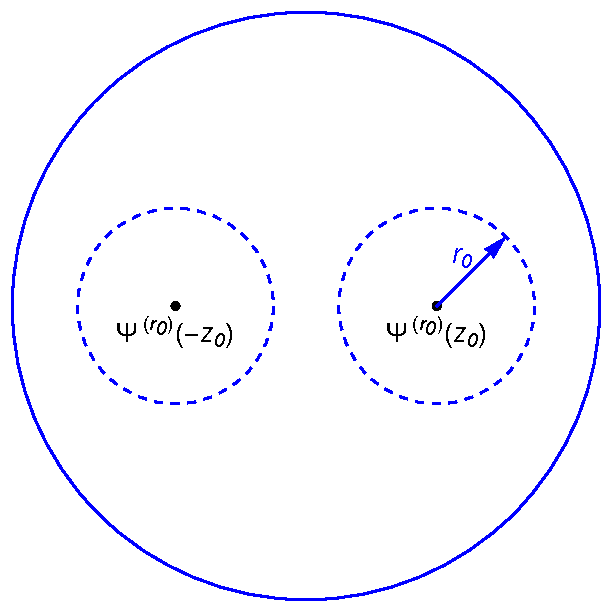
\includegraphics[width=.3\textwidth]{figures/flat2vertex.pdf}
\caption{The flat 2-string bracket (\ref{twostringbrackbos}) is constructed from the operator product of a pair of string fields $\Psi$, rescaled by $r_0$ and inserted at $-z_0$ and $z_0$ respectively.}\label{fig:flat2vertex}
\end{figure}


Explicitly, the flat 2-string bracket may be taken to be
\ie\label{twostringbrackbos}
[\Psi^{\otimes 2}] = b_0^-\mathbb{P}^- \left[ (r_0^{L_0^+} \Psi)(z_0)  (r_0^{L_0^+}) \Psi(-z_0) \right],
\fe
where we have set $|q_1|=|q_2|=r_0$, and $z_1=-z_2=z_0$, subject to $|z_0|+r_0<1$. The product of string fields on the RHS of (\ref{twostringbrackbos}) is understood as the ordinary operator product. The flat 3-string bracket then takes the form
\ie\label{threestringbrackbos}
[\Psi^{\otimes 3}] = {1\over -2\pi i} b_0^-\mathbb{P}^- \int_{{\cal D}_{0,4}} dt\wedge d\bar t \, {\cal B}_{\bar t} {\cal B}_t \prod_{i=1}^3 (|q_i|^{L_0^+} \Psi)(z_i) ,
\fe
where $q_i=q_i(t, \bar t)$ and $z_i=z_i(t, \bar t)$ are functions of the complex modulus $t$ over the domain ${\cal D}_{0,4}$, with 
${\cal B}_t = - \sum_{i=1}^3 \left[ {\partial z_i\over \partial t} b_{-1}^{(z_i)} + {\partial\log q_i\over \partial t} b_0^{(z_i)} + {\partial \bar z_i\over \partial t} \widetilde b_{-1}^{(\bar z_i)} + {\partial\log\bar q_i\over \partial t} \widetilde b_0^{(\bar z_i)} \right]$.
We may, for instance, take $t$ to be the cross ratio $z_{31}/z_{21}$, in which case the domain ${\cal D}_{0,4}$ is parameterized as
\ie
{\cal D}_{0,4} = \left\{ t\in \mathbb{C}: |t-\tfrac{1}{2}|, |\tfrac{1}{t} - \tfrac{1}{2}|, |\tfrac{1}{1-t} - \tfrac{1}{2}| < r_0^{-1} \right\}.
\fe
On one of the boundary components $|t-\tfrac{1}{2}|=r_0^{-1}$, the matching condition is
\ie{}
& |q_1|=|q_2|=r_0^2, ~~~|q_3|=r_0,
\\
& z_1 = - z_0 {t+{1\over 2}\over t-{1\over 2}}, ~~~ z_2 = - z_0 {t-{3\over 2}\over t-{1\over 2}},~~~ z_3 = z_0.
\fe
The matching condition on the two other components of $\partial {\cal D}_{0,4}$ is similar with the roles of $z_1, z_2, z_3$ permuted.


\begin{figure}[h!]
\centering
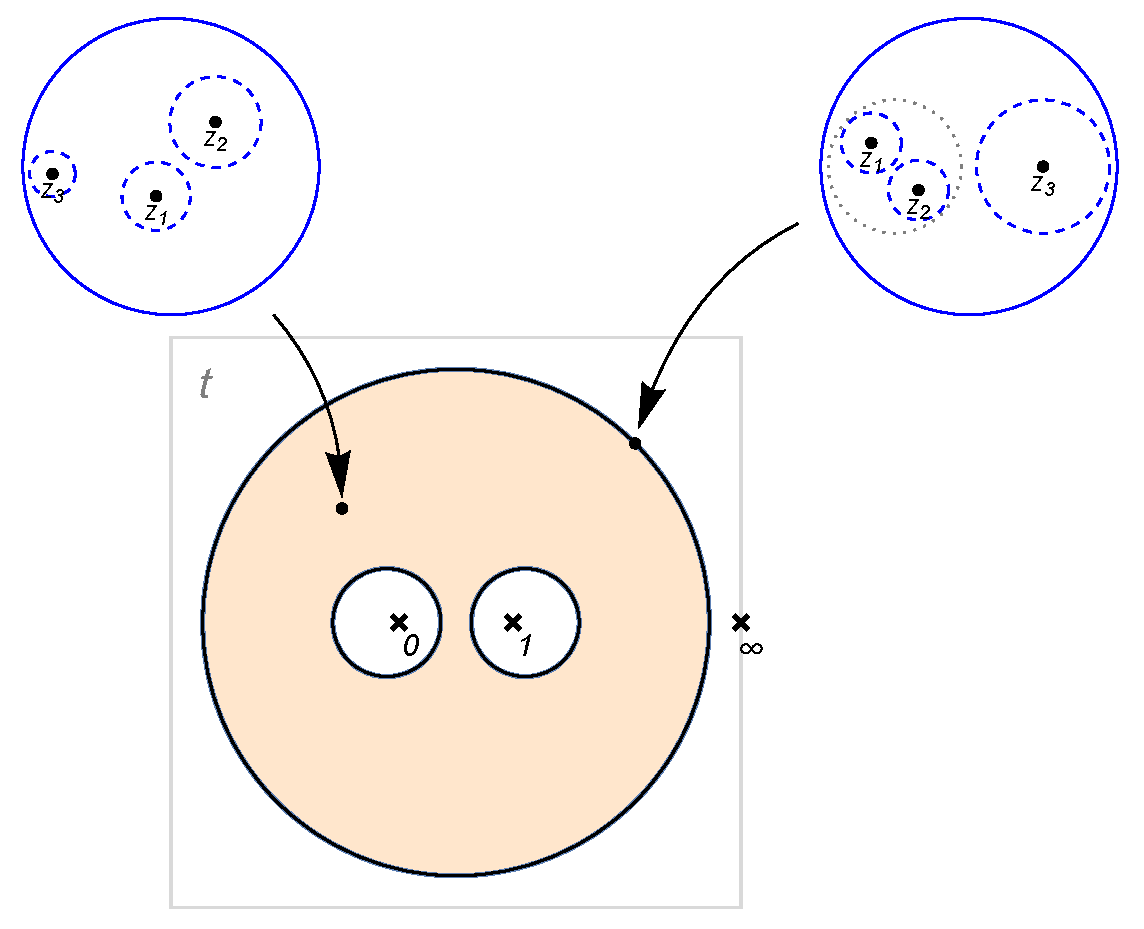
\includegraphics[width=.6\textwidth]{figures/flat3vertex.pdf}
\caption{The flat 3-string bracket (\ref{threestringbrackbos}) involves three string fields $\Psi$, rescaled by $q_i(t, \bar t)$ and inserted at $z_i(t, \bar t)$ in the unit disc, $i=1,2,3$. The integration domain ${\cal D}_{0,4}$ on the complex $t$-plane is shown as the orange shaded region.}\label{fig:flat3vertex}
\end{figure}


\subsubsection{Massless effective string field equations}
\label{sec:masslesseffsftbos}

In analyzing perturbative solutions to (\ref{clsfteom}), it will be useful to split the string field $\Psi$ into ``light'' and ``heavy'' components,
\ie\label{psiw}
\Psi = W + (1- \mathbb{P}^+) \Psi,~~~~ W \equiv \mathbb{P}^+\Psi,
\fe
where $\mathbb{P}^+$ is the projector that takes ${\cal H}_0$ to its subspace with weight $|L_0^+|\leq \varepsilon$, for a sufficiently small positive parameter $\varepsilon$. In the weak field strength or slow-varying field approximation, we may take $\varepsilon\sim {\cal O}(\A'/L^2)$, where $L$ is the length scale of massless field fluctuations in the spacetime, and $W$ in (\ref{psiw}) may be interpreted as the massless component of the string field. 

Working in a relaxed version of the Siegel gauge
\ie\label{relaxedsiegel}
b_0^+ (1-\mathbb{P}^+) \Psi = 0,
\fe
we can solve the heavy component of $\Psi$ from (\ref{clsfteom}) by iterating 
\ie\label{psiiter}
(1-\mathbb{P}^+) \Psi = - {b_0^+\over L_0^+}  \sum_{n+m\geq 2} {1\over n! m!} (1-\mathbb{P}^+)[W^{\otimes n} \otimes ((1-\mathbb{P}^+)\Psi)^{\otimes m}].
\fe
The SFT equation (\ref{clsfteom}) then reduces to an equation of the massless string field $W$, of the form
\ie\label{weom}
Q_B W + \sum_{n=2}^\infty {1\over n!} [W^{\otimes n}]' = 0,
\fe
where the {\it effective} string bracket $[\,\cdot\,]'$ satisfy $L_\infty$ relations similar to (\ref{linfty}) (with $\Psi$ replaced by $W$, and $[\,\cdot\, ]$ replaced by $[\,\cdot\, ]'$). Explicitly, the 2- and 3-string effective brackets are
\ie\label{twothresctbra}
& [W^{\otimes 2}]' =   \mathbb{P}^+ [W^{\otimes 2}],
\\
& [W^{\otimes 3}]' = \mathbb{P}^+ [W^{\otimes 3}] - 3  \mathbb{P}^+ \left[W\otimes \Big({b_0^+\over L_0^+} (1-\mathbb{P}^+) [W^{\otimes 2}] \Big)\right] .
\fe
The gauge condition (\ref{relaxedsiegel}) leaves residual gauge transformations generated by a string field $\Lambda$ that satisfies
\ie\label{residual}
b_0^+ (1-\mathbb{P}^+) \delta_\Lambda\Psi=0,
\fe
where $\delta_\Lambda \Psi = Q_\Psi\Lambda$ as in (\ref{gaugeclsft}). Now splitting $\Lambda$ into its light and heavy components,
\ie
\Lambda = \Omega + (1-\mathbb{P}^+)\Lambda,~~~~ \Omega \equiv \mathbb{P}^+ \Lambda,
\fe
we can further impose the relaxed Siegel condition on $\Lambda$ itself, namely
\ie
b_0^+ (1-\mathbb{P}^+) \Lambda = 0.
\fe
The massive component of $\Lambda$ is then solved from (\ref{residual}) by iterating
\ie
(1-\mathbb{P}^+)\Lambda &= -  \sum_{n=1}^\infty {1\over n!} {b_0^+\over L_0^+}(1-\mathbb{P}^+)[(W+(1-\mathbb{P}^+)\Psi)^{\otimes n}\otimes (\Omega + (1-\mathbb{P}^+)\Lambda)],
\fe
where $(1-\mathbb{P}^+)\Psi$ is determined by $W$ through (\ref{psiiter}). In the end, the light component of the gauge variation $\delta_\Lambda\Psi$ can be viewed as a gauge transformation of the massless string field $W$,
\ie
\delta_\Omega W &\equiv \mathbb{P}^+(\delta_\Lambda\Psi)
\\
&= Q_B \Omega + \sum_{n=1}^\infty {1\over n!} \mathbb{P}^+[ (W+ (1-\mathbb{P}^+) \Psi)^{\otimes n}\otimes (\Omega + (1-\mathbb{P}^+) \Lambda)]
\\
&= Q_B \Omega + \sum_{n=1}^\infty {1\over n!} [W^{\otimes n}\otimes \Omega]',
\fe
in a form similar to (\ref{genbrstga}) (with the string fields replaced by their massless versions and the string bracket replaced by the effective brackets).

\subsubsection{Diffeomorphism transformation of string fields}

Let us consider a worldsheet-parity even massless string field of ghost number 2, whose general form is
\ie\label{wsfield}
W = {1\over \A'} c\wt c  h_{\mu\nu}(X) \partial X^\mu \bar\partial X^\nu + \phi(X) {1\over 2} (c\partial^2 c - \wt c \bar\partial^2 \wt c) + A_\mu(X) c_0^+ (c \partial X^\mu - \wt c \bar\partial X^\mu),
\fe
where $h_{\mu\nu}(x)$ is symmetric with respect to $(\mu\nu)$, and $h_{\mu\nu}(x), \phi(x), A_\mu(x)$ are assumed to be slow-varying functions on $\mathbb{R}^{1,25}$. For the purpose of understanding the role of diffeomorphism invariance, we will not impose the Siegel gauge condition on $W$.\footnote{In fact, $A_\mu(x)$ is an auxiliary field, constrained by the SFT equation to be $A_\mu = \partial_\mu\phi + {1\over 2} \partial^\nu h_{\mu\nu} + \cdots$.}

The relevant gauge transformation on $W$ is generated by a ghost number 1 worldsheet-parity even string field
\ie\label{omvgaugf}
\Omega = {1\over \A'} V_\mu(X)  (c\partial X^\mu - \wt c \bar\partial X^\mu),
\fe
of the form
\ie\label{deltome}
\delta_\Omega W &\equiv {1\over \A'} c\wt c  \delta_\Omega h_{\mu\nu}(X) \partial X^\mu \bar\partial X^\nu + \delta_\Omega \phi(X) {1\over 2} (c\partial^2 c - \wt c \bar\partial^2 \wt c) + \sqrt{2\over\A'} \delta_\Omega A_\mu(X) c_0^+ (c \partial X^\mu - \wt c \bar\partial X^\mu)
\\
& = Q_B \Omega + [W\otimes \Omega]' + \cdots,
\fe
where $\cdots$ stands for higher order terms in $W$. A straightforward but somewhat tedious calculation of the first two terms in the second line of (\ref{deltome}), using the {\it flat string bracket} defined in section \ref{sec:flatbos}, gives
\ie\label{omegah}
\delta_\Omega h_{\mu\nu} &= - \partial_\mu V_\nu - \partial_\nu V_\mu - V^\rho \partial_\rho h_{\mu\nu} + {1\over 4} V^\rho(\partial_\mu h_{\rho\nu} + \partial_\nu h_{\rho\mu}) 
\\
&~~~ + {1\over 2} (\partial^\rho V_\mu h_{\rho\nu} + \partial^\rho V_\nu h_{\rho\mu})- {1\over 4} (\partial_\mu V^\rho h_{\rho\nu} + \partial_\nu V^\rho h_{\rho\mu}) +\cdots,
\\
\delta_\Omega \phi &= {1\over 2} \partial_\mu V^\mu - {3\over 4} V^\mu\partial_\mu \phi - {1\over 4} V^\mu A_\mu +\cdots,
\\
\delta_\Omega A_\mu &= - {1\over 2} \Box{V}_\mu - {3\over 4} V^\nu \partial_\nu A_\mu + {3\over 4} A^\nu \partial_\nu V_\mu +{1\over 4} V^\nu \partial_\mu A_\nu - {1\over 4} A_\nu \partial_\mu V^\nu +\cdots,
%&= (\delta_\mu^\rho - {1\over 2} h_\mu{}^\rho)( \delta_\nu^\sigma -{1\over 2} h_\nu{}^\sigma)(-\nabla_\rho^{(h)} \varepsilon_\sigma -\nabla_\sigma^{(h)} \varepsilon_\rho ) +\cdots.
\fe
where we have omitted higher order terms in the string field as well as terms involving more $X^\mu$-derivatives that are suppressed in the slow-varying field approximation. The first equation of (\ref{omegah}) can be organized in the form
\ie\label{omegahtwo}
\delta_\Omega (h_{\mu\nu} + {1\over 2} h_{\mu\rho} h^\rho{}_\nu) = -\nabla_\mu^{(h)} \varepsilon_\nu -\nabla_\nu^{(h)} \varepsilon_\mu  +\cdots,
\fe
where $\varepsilon^\mu$ is the vector field
\ie\label{epsvec}
\varepsilon^\mu = V^\mu - {1\over 4} h^\mu{}_{\rho} V^\rho +\cdots 
\fe
and $\nabla^{(h)}$ is the covariant derivative defined with respect to the metric $\delta_{\mu\nu} + h_{\mu\nu}$.
%\ie
%-\nabla_\rho^{(h)} \varepsilon_\sigma -\nabla_\sigma^{(h)} \varepsilon_\rho = -\partial_\mu \varepsilon_\nu -\partial_\nu \varepsilon_\mu - \varepsilon^\rho \partial_\rho h_{\mu\nu} - \partial_\mu \varepsilon^\rho h_{\rho \nu} - \partial_\nu \varepsilon^\rho h_{\rho \mu} +\cdots.
%\fe
To the order calculated thus far, (\ref{omegahtwo}) takes the form of the variation of a Riemannian metric tensor $G_{\mu\nu}$ with respect to the diffeomorphism vector field $\varepsilon^\mu$, provided that we identify
\ie\label{gmunuidh}
G_{\mu\nu} = \delta_{\mu\nu} + h_{\mu\nu} + {1\over 2} h_{\mu\rho} h^\rho{}_\nu +\cdots.
\fe
We can interpret (\ref{gmunuidh}) as the relation between a covariant spacetime metric $G_{\mu\nu}$ and the string field (in the frame defined by the flat string brackets), and (\ref{epsvec}) as the relation between the diffeomorphism vector field and the SFT gauge parameter. In a similar way, one finds that
\ie\label{dilatonphiid}
\Phi \equiv \phi + {1\over 4} h + {1\over 32} h^{\mu\nu} h_{\mu\nu} +\cdots
\fe
transforms as a (massless) scalar field, and can therefore be identified with the dilaton.


The above analysis can be generalized to include the $B$-field, by adding to (\ref{wsfield}) the worldsheet-parity-odd massless string field
\ie
\wt W = {1\over \A'} c\wt c b_{\mu\nu}(X) \partial X^\mu \bar\partial X^\nu + \wt\phi(X) {1\over 2} (c\partial^2 c + \wt c \bar\partial^2 \wt c) + \wt A_\mu(X) c_0^+ (c \partial X^\mu + \wt c \bar\partial X^\mu),
\fe
where $b_{\mu\nu}(x)$ is anti-symmetric with respect to $[\mu\nu]$, and $b_{\mu\nu}(x), \wt \phi(x), \wt A_\mu(x)$ are assumed to be slow-varying functions on $\mathbb{R}^{1,25}$, and adding to (\ref{omvgaugf}) the ghost number 1 string field 
\ie\label{wtomgh}
\wt \Omega = {1\over \A'} K_\mu(X) (c\partial X^\mu + \wt c \bar\partial X^\mu) .
\fe
By comparing with the expected transformation of a covariant anti-symmetric tensor $B_{\mu\nu}$ under diffeomorphism, as well as its 1-form gauge variation $\delta B_{\mu\nu} = \partial_\mu\theta_\nu - \partial_\nu\theta_\mu$, one can determine the relation between the covariant massless spacetime fields $G_{\mu\nu}, B_{\mu\nu}, \Phi$ and the string field (in the flat bracket frame), up to quadratic order, as
\ie\label{gphiid}
& G_{\mu\nu} = \delta_{\mu\nu} + h_{\mu\nu} + {1\over 2} h_{\mu\rho} h^\rho{}_\nu + {1\over 2} b_{\mu\rho} b^{\rho}{}_\nu + \cdots,
\\
& B_{\mu\nu} = b_{\mu\nu} + {1\over 2} h_\mu{}^\rho b_{\rho\nu} + {1\over 2} b_{\mu\rho} h^\rho{}_\nu+\cdots,
\\
& \Phi = \phi + {1\over 4} h + {1\over 32} h^{\mu\nu} h_{\mu\nu} - {3 \over 32} b^{\mu\nu} b_{\mu\nu} + \cdots.
\fe
The diffeomorphism vector field $\varepsilon^\mu$ and the 1-form gauge parameter $\theta_\mu$ are related to the string field gauge parameters as
\ie{}
& \varepsilon^\mu =  V^\mu - {1\over 4} h^\mu{}_{\rho} V^\rho + {1\over 4} b^\mu{}_{\rho} K^\rho  +\cdots ,
\\
& \theta_\mu = K_\mu + {1\over 4} h_{\mu\rho} K^\rho - {1\over 4} b_{\mu\rho} V^\rho +\cdots.
\fe

\subsection{Background independence}
\label{sec:backinddiffeo}

The formulation of SFT thus far is based on a worldsheet CFT that describes a specific background of the bosonic string theory. A deformation of the background may be represented in two different ways: (1) an (exactly marginal) deformation of the worldsheet matter CFT, or (2) turning on a nontrivial solution of the SFT equation of motion. The idea of {\it background independence} is that (1) and (2) should be equivalent. This is evident at the linearized level: a marginal deformation of the matter CFT is generated by a weight $(1,1)$ primary $V^{\rm m}$, giving rise to a string field $\Psi = c\widetilde c V^{\rm m}$ that satisfies the linearized equation of motion $Q_B\Psi=0$; this is none other than the OCQ representative of the BRST cohomology in the Siegel gauge.

In order to understand the string field theories related by CFT deformations, it will be useful to reformulate the SFT path integral of section \ref{bvsftsec} in terms of general coordinates on the string field space, as follows.\footnote{The exposition of background independence of closed string field theory in this section follows closely Sen and Zwiebach,
Nucl. Phys. B \textbf{414}, 649-714 (1994) \cite{Sen:1993mh}; Nucl. Phys. B \textbf{423}, 580-630 (1994) \cite{Sen:1993kb}.} Given a worldsheet CFT $x$, let ${\cal H}_x$ be the BV space of closed string fields, equipped with the symplectic form $\omega_x$ and the action functional $S_x$ that satisfies the quantum master equation
\ie
\Delta_x e^{-S_x} = 0.
\fe
In a general coordinate system $\psi^i$ on ${\cal H}_x$, the operator $\Delta_x$ is expressed as
\ie
\Delta_x A \equiv {(-)^{|\psi^i|+1}\over 2\rho_x} {\partial\over\partial\psi^i} \left( \rho_x\,  \omega_x^{ij} {\partial\over\partial \psi^j} \right) A,
\fe
where $(-)^{|\psi^i|}$ stands for the Grassmann parity of $\psi^i$, and $\rho$ is a density function that appears in the functional measure on ${\cal H}_x$,
\ie
d\mu_x = \rho_x \prod_i d\psi^i.
\fe
Note that $d\mu_x$ is an {\it integral form} rather than a differential form,\footnote{Under a coordinate transformation, $d\mu$ transforms by the Berezinian (\ref{berezianform}) rather than a Jacobian factor.} and does not arise from the symplectic form $\omega_x$ (which squares to zero). An essential consistency requirement on $\rho_x$ is that $\Delta_x^2=0$. We can choose the string field coordinates $\psi^i$ so that $\rho_x$ is field-independent (but may nonetheless depend on $x$).

A general gauge-fixed SFT path integral takes the form
\ie\label{lxsxdint}
\int_{L_x} d\lambda_x \, e^{-S_x},
\fe 
where $L_x\subset {\cal H}_x$ is a Lagrangian submanifold, equipped with the measure $d\lambda_x$ defined by the following property. Let $e_\A$ be a basis of the tangent space of $L$, and $f^\A$ a set of vectors that obey $\omega(e_\A, f^\B) = \delta_\A^\B$, then the volume elements defined by $d\lambda$ and $d\mu$ are related by
\ie\label{defmeasure}
d\lambda(e_1,e_2,\cdots) = \sqrt{d\mu(e_1, e_2,\cdots, f^1, f^2,\cdots)}.
\fe
Now given two worldsheet CFTs $x$ and $y$, the background independence of SFT amounts to the existence of a diffeomorphism between the string field spaces
\ie\label{fxydiff}
F_{x,y}: ~{\cal H}_x\to {\cal H}_y
\fe
such that
\ie\label{bckindcond}
& \omega_x = F_{x,y}^*\omega_y,
\\
& d\mu_x e^{-2S_x} = F_{x,y}^*(d\mu_y e^{-2 S_y}).
\fe
These conditions ensure the equivalence of observables defined by the SFT path integral, namely
\ie
\left\langle A\right\rangle_y = \int_{L_y} d\lambda_y \, e^{-S_y} A = \int_{F_{x,y}^*L_y} d\lambda_x \, e^{-S_x} F_{x,y}^*A = \left\langle F_{x,y}^*A\right\rangle_x,
\fe
where the gauge condition is transformed accordingly, $L_x = F_{x,y}^* L_y$.

We will aim to construct the infinitesimal form of (\ref{fxydiff}) associated with a marginal deformation of the CFT, the latter represented in terms of the coordinates $x^\mu$ on the space of CFTs (also known as the ``conformal manifold'') as $y^\mu=x^\mu+\delta x^\mu$. We can work with string field coordinates $\psi_x^i$ in which the components of the symplectic form $(\omega_x)_{ij}\equiv \omega_{x,ij}$ are field-independent, and write the infinitesimal diffeomorphism (\ref{fxydiff}) as
\ie
F^i_{x,x+\delta x}(\Psi) = \psi^i + \delta x^\mu f_{x,\mu}^i(\Psi).
\fe
The infinitesimal form of the condition (\ref{bckindcond}) reads
\ie\label{diffinfsft}
& {\partial\omega_{x,ij}\over \partial x^\mu} + {\partial f^{i'}_{x,\mu}\over \partial \psi^i} \omega_{x,i' j} + \omega_{x,ij'} {\partial_R f_{x,\mu}^{j'} \over \partial \psi^j} = 0,
\\
& - {\partial S_x\over \partial x^\mu} - {\partial_R S_x\over \partial \psi_x^i} f^i_{x,\mu} + {1\over 2} {\partial \log\rho_x\over \partial x^\mu} + {1\over 2} {\rm str} \left( {\partial f^i_{x,\mu} \over \partial \psi_x^j} \right) = 0,
\fe
where ${\rm str}$ in the second line stands for the super trace (with respect to the indices $i, j$). The first equation of (\ref{diffinfsft}) is satisfied by
\ie
f^i_{x,\mu}(\Psi) = -\Gamma^i_{x,\mu j} \psi^j - \omega_x^{ij} {\partial U_{x,\mu} \over \partial \psi^j},
\fe
where $\Gamma^i_{x,\mu j}$ is a suitable field-independent connection that satisfies
\ie\label{connsft}
{\partial\omega_{x,ij}\over \partial x^\mu} - (-)^{|\psi^i|(|\psi^{i'}|+1)} \Gamma_{x,\mu i}^{i'} \omega_{x,i' j} - \omega_{x,ij'} \Gamma_{x,\mu j}^{j'}  = 0,
\fe
and $U_{x,\mu}$ is a suitable functional of the string field $\Psi_x$.
The second equation of (\ref{diffinfsft}) is equivalently written as
\ie\label{umusft}
- D_\mu S_x + \Delta_x U_{x,\mu} + (S_x, U_{x,\mu})  = - {1\over 2} {\partial \log\rho_x\over \partial x^\mu} + {1\over 2} {\rm str} (\Gamma_{x,\mu}) ,
\fe
where
\ie\label{connsac}
D_\mu S_x \equiv {\partial S_x\over \partial x^\mu} - {\partial_R S_x\over \partial \psi^i} \Gamma^i_{x,\mu j}\psi^j .
\fe
Our aim therefore amounts to identifying the connection $\Gamma_{x,\mu}$ and constructing $U_{x,\mu}[\Psi_x]$ that obey (\ref{connsft}) and (\ref{umusft}).

Before proceeding, we need to introduce a few more notations. Suppose the CFT deformation $x^\mu\to x^\mu+\delta x^\mu$ is generated by the weight $(1,1)$ matter CFT primary ${\cal O}_\mu$. We define the genus $h$ string vertex with the insertion of ${\cal O}_\mu$ at a ``special puncture'' (indicated by $\bullet$ in the subscript),
\ie\label{specaipun}
\{\Psi^{\otimes n};{\cal O}_\mu \}_{h,n\bullet} &\equiv - {1\over (-2\pi i)^{3h-2+n}}\int_{\Gamma_{h,n\bullet}} \left\langle e^{\cal B} \prod_{i=1}^n [\Psi(0)]^{f_i} \big[c\widetilde c {\cal O}_\mu(0) \big]^{f_{n+1}} \right\rangle
\\
&= - {1\over (-2\pi i)^{3h-3+n}}\int_{\Gamma_{h,n}} \left\langle e^{\cal B} \prod_{i=1}^n [\Psi(0)]^{f_i} \int {d^2z\over 2\pi} {\cal O}_\mu(z, \bar z) \right\rangle,
\fe
for $(h=0,n\geq 3)$, $(h=1,n\geq 1)$, and $(h\geq 2,n\geq 0)$, where $\Gamma_{h,n\bullet}$ is a $(6h-6+2n+2)$-dimensional chain in $\widehat{\cal P}_{h,n+1}$, constructed as the $n$-punctured surface $\Sigma$ with coordinate maps $f_1,\cdots, f_n$ on the discs $D_1,\cdots, D_n$ as in $\Gamma_{h,n}$, and an additional $(n+1)$-th puncture at any point in $\Sigma\backslash \sqcup_i D_i$, with an arbitrarily chosen coordinate map $f_{n+1}$. Moreover, we define in the $(h=0, n=2)$ case,
\ie\label{gamzeodot}
\{\Psi^{\otimes 2};{\cal O}_\mu \}_{0,2\bullet} \equiv  \langle\langle \Psi| c\widetilde c {\cal O}_\mu(1) |\Psi\rangle.
\fe
The corresponding 0-chain in $\widehat{\cal P}_{0,3}$ is denoted $\Gamma_{0,2\bullet}$. 

%Here and henceforth we will omit the subscript $x$ as the dependence on $x$ is implicit. 
Next, we write the SFT action as
\ie\label{sftactonevac}
S[\Psi] = S_{0,2}[\Psi] + S_{1,0} + S'[\Psi],
\fe
where $S_{0,2}[\Psi] = {1\over 2} \langle\langle\Psi|c_0^-Q_B|\Psi\rangle$ is the kinetic term, $S'[\Psi]=\sum_{n=1}^\infty \sum_{h=0}^\infty {1\over n!} \{\Psi^{\otimes n} \}_{h,n}$ is the sum of all vertices with $(h=0,n\geq 3)$, $(h=1,n\geq 1)$, $(h\geq 2,n\geq 0)$. We have also included on the RHS of (\ref{sftactonevac}) the genus one vacuum contribution $S_{1,0}$, 
\ie
S_{1,0} =  - \int_{\Gamma_{1,0}} {id\tau\wedge d\bar\tau\over 2\tau_2} |\eta(\tau)|^4 Z_{\rm m}(\tau,\bar\tau),
\fe
where the integrand takes the same form as in (\ref{aoneform}). $\Gamma_{1,0}$ is an integration chain in the moduli space ${\cal M}_{1,0}$, to be determined. It follows that
\ie\label{sonezeros}
-{\partial S_{1,0}\over \partial x^\mu} = {1\over 2\pi i} \int_{\Gamma_{1,0\bullet}} \left\langle e^{\cal B} c\widetilde c {\cal O}_\mu \right\rangle \equiv \{{\cal O}_\mu\}_{1,0\bullet},
\fe
where $\Gamma_{1,0\bullet}$ is a 2-chain in $\widehat{\cal P}_{1,1}$, which upon forgetting the (special) puncture reduces to $\Gamma_{1,0}$.

A canonical connection $\Gamma_{x,\mu j}^i$ on the fibration of ${\cal H}_x$ over the space of CFTs is defined by the property that the parallel transport along any direction of CFT deformation preserves the basis of states defined by inserting $\psi^i$ at the center of a unit disc on which the CFT remains undeformed, whereas the deformation of the CFT is represented by integrating ${\cal O}_\mu$ outside of the unit disc. This connection preserves the symplectic form on ${\cal H}_x$, i.e. (\ref{connsft}) is satisfied. Moreover,  taking the covariant derivative $D_\mu$ (\ref{connsac}) with respect to the canonical connection amounts to integrating the insertion of ${\cal O}_\mu$ over $\Sigma\backslash \sqcup_i D_i$ in the string vertices, giving\footnote{The $h=0$, $n=2$ component of (\ref{dmuseq}), namely $- D_\mu S_{0,2} = {1\over 2} \{\Psi^{\otimes 2};{\cal O}_\mu \}_{0,2\bullet}$, follows from the deformation of the stress-energy tensor that appears in the BRST charge.}
\ie\label{dmuseq}
- D_\mu S = \sum_{n=0}^\infty \sum_{h=0}^\infty {1\over n!} \{ \Psi^{\otimes n}; {\cal O}_\mu \}_{h,n\bullet},
\fe
where the sum on the RHS includes all terms with $(h=0, n\geq 2)$ and $(h\geq 1, n\geq 0)$. The functional $U_\mu[\Psi]$
is constructed as
\ie
U_\mu[\Psi] = \langle\langle \Psi| c_0^- | c\widetilde c {\cal O}_\mu \rangle
+ \sum_{h,n} {1\over (n-1)! (-2\pi i)^{3h-3+n}}\int_{{\cal U}_{h,n-1|1}} \left\langle e^{\cal B} \prod_{i=1}^{n-1} [\Psi(0)]^{f_i}\, \big[ c\widetilde c {\cal O}_\mu(0) \big]^{f_n} \right\rangle,
\fe
where ${\cal U}_{h,n-1|1}$ is a $(6h-6+2n)+1$ dimensional integration chain in $\widehat{\cal P}_{h,n}$ that is symmetric with respect to the first $(n-1)$ punctures, and is nonzero only for $(h=0,n\geq 3)$ and $(h\geq 1, n\geq 2)$. The condition (\ref{umusft}) would be satisfied provided
\ie\label{logrhoeq}
{1\over 2\pi i} \int_{\widehat\varrho({\cal U}_{0,2|1})+\Gamma_{1,1}- \Gamma_{1,0\bullet}} \left\langle e^{\cal B} c\widetilde c {\cal O}_\mu \right\rangle - {1\over 2} {\partial \log\rho_x\over \partial x^\mu} + {1\over 2} {\rm str} (\Gamma_{x,\mu}) = 0,
\fe
together with the geometric condition
\ie\label{uhneq}
 \partial {\cal U}_{h,n|1} = \widehat\varrho( {\cal U}_{h-1,n+2|1}) + \sum_{g=0}^{h}\sum_{\A\sqcup\B=\{1,\cdots,n\}} \widehat\varrho_{\A,\B}(\Gamma_{g,m}, {\cal U}_{h-g,n-m+2|1}) + \Gamma_{h,n+1} - \Gamma_{h,n\bullet} ,
\fe
for $(h=0, n\geq 2)$, $(h=1, n\geq 1)$, and $(h\geq 2, n\geq 0)$. Here we have adopted the notation
\ie{}
& \widehat\varrho( {\cal U}_{h,n|1}) \equiv \widehat\varrho \left( \widetilde{\cal U}_{h-1,n+2|1} \times \{q:|q|=1\} \right),
\\
& \widehat\varrho_{\A,\B}(\Gamma_{g,m}, {\cal U}_{h-g,n-m+2|1}) \equiv \widehat\varrho_{\A,\B} \left( \widetilde \Gamma_{g,m}\times \widetilde{\cal U}_{h-g,n-m+1|1} \times \{q:|q|=1\} \right),
\fe
where the RHS, $\widehat\varrho$ stands for self-plumbing on the first pair of punctures, and $\widehat\varrho_{\A,\B}$ stands for the plumbing fixture construction with the punctures labeled by $\A$ distributed on the first surface, and those labeled by $\B$ on the second surface. These are similar to the plumbing constructions appearing in (\ref{stringvcomp}) except that the special puncture (where $c\widetilde c{\cal O}_\mu$ is inserted) is untouched. 

The ($h=0, n=2$) case of (\ref{uhneq}) amounts to
\ie
\partial {\cal U}_{0,2|1} = \Gamma_{0,3} - \Gamma_{0,2\bullet}.
\fe
This can be solved by taking ${\cal U}_{0,2|1}$ to be a 1-chain in $\widehat{\cal P}_{0,3}$ that begins at $\Gamma_{0,2\bullet}$ and ends at $\Gamma_{0,3}$. Consequently, $\widehat\varrho({\cal U}_{0,2|1})$ interpolates between $\partial\Gamma_{1,1}=-\widehat\varrho(\Gamma_{0,3})$ (by the geometric master equation) and $\widehat\varrho(\Gamma_{0,2\bullet})$, the latter corresponding to singular tori with a special puncture. The 2-chain $\widehat\varrho({\cal U}_{0,2|1})+\Gamma_{1,1}$ covers the moduli space ${\cal M}_{1,1}$, and therefore (\ref{logrhoeq}) reduces to
\ie
{\partial\over \partial x^\mu} \left[ \int_{{\cal M}_{1,0}} {id\tau\wedge d\bar\tau\over 2\tau_2} |\eta(\tau)|^4 Z_{\rm m}(\tau,\bar\tau) + S_{1,0} - {1\over 2} { \log\rho_x}\right] + {1\over 2} {\rm str} (\Gamma_{x,\mu}) = 0.
\fe
This is solved by choosing the density $\rho_x$ to be precisely such that the 1-loop SFT functional integral agrees with the 1-loop partition function in the on-shell formulation, namely
\ie
\int_{L_x} d\lambda_x\, e^{-S_{0,2}[\Psi] - S_{1,0}} = \exp\left[ \int_{{\cal M}_{1,0}} {id\tau\wedge d\bar\tau\over 2\tau_2} |\eta(\tau)|^4 Z_{\rm m}(\tau,\bar\tau) \right].
\fe
The remaining equations of (\ref{uhneq}) can be solved inductively with respect to $h$ and $n$, as the RHS of (\ref{uhneq}) can be shown to be trivial in homology and thus the interpolating chain ${\cal U}_{h,n|1}$ exists, and moreover can be arranged to be symmetric with respect to its $n$ regular punctures.





%\Delta_x U_{x,\mu} + (S_x, U_{x,\mu}) + \sum_{n=1}^\infty \sum_{h=0}^\infty {1\over n!} \{ \Psi^{\otimes n}; {\cal O}_\mu \}_{h,n\bullet} = 0.















\newpage

\section{Quantization of superstrings}
\label{superstringsec}

\subsection{Supersymmetric extension of Polyakov's action}
\label{sec:superbrink}

A supersymmetric version of Polyakov's worldsheet theory is formulated in terms of the dynamical metric $g_{ab}$, its super-partner the fermionic gravitino field $\chi_{a\A}$ (where $\A=\pm$ is a worldsheet spinor index), the embedding coordinate fields $X^\mu$ and their super-partner the fermionic Majorana spinor fields $\psi_\A^\mu$, $\mu=0,1,\cdots,D-1$. The superstring worldsheet action, in Euclidean signature, is\footnote{In the kinetic term for $\psi^\mu$, the spin-covariant derivative $\nabla_a^{\rm spin}$ can be traded for the ordinary derivative $\partial_a$. See however the comments around (\ref{fermeom}).}
\ie\label{superp}
&S[g, \chi, X, \psi] 
\\
&= {1\over 4\pi} \int d^2\sigma \sqrt{\det g} \left[ {1\over \A'}  g^{ab} \partial_a X^\mu \partial_b X_\mu + i \psi^\mu \Gamma^a \partial_a \psi_\mu -i  (\chi_a \Gamma^b \Gamma^a \psi^\mu) \left( {1\over \sqrt{\A'}} \partial_b X_\mu - {i\over 4} \chi_b \psi_\mu \right) \right].
\fe
Here we adopt the following conventions: the metric $g_{ab}$ is expressed in terms of the frame field $e^i{}_a$ as $g_{ab} = \delta_{ij} e^i{}_a e^j{}_b$, and the coordinate-dependent matrices $\Gamma^a$ are related to the constant two-dimensional Dirac gamma matrices $\hat \Gamma^i$ by $\Gamma^a = e_i{}^a \hat \Gamma^i$, where $e_i{}^a$ is the inverse frame field satisfying $e_i{}^a e^j{}_a = \delta_i^j$. Spinor indices are raised or lowered according to $\zeta^\A \equiv \epsilon^{\A\B}\zeta_\B$, with $\epsilon^{+-} = \epsilon_{+-}=1$, and contracted according to $(\zeta\eta) \equiv \zeta^\A\eta_\A$, $(\zeta\Gamma^a \eta) \equiv \zeta^\A (\Gamma^a)_\A{}^\B \eta_\B$, etc. Further details on the convention for spinor fields on a two-dimensional curved worldsheet are given in Appendix \ref{freeferm}. 

The action (\ref{superp}) is subject to a number of gauge redundancies: diffeomorphism, super-diffeomorphism, Weyl symmetry, and super-Weyl symmetry. The super-diffeomorphism transformation takes the form 
\ie\label{localsusyws}
& \delta e^i{}_a = i \varepsilon \hat\Gamma^i \chi_a,~~~\delta g_{ab} = i \varepsilon (\Gamma_a \chi_{b} + \Gamma_b \chi_{a}),
\\
& \delta \chi_{a} =  2 \nabla_a^{\rm spin} \varepsilon + {i\over 4}(\chi_a \Gamma_{ij}\Gamma^b \chi_b) (\Gamma^{ij}\varepsilon),
\\
& \delta X^\mu = i \sqrt{\A'} \varepsilon \psi^\mu,
\\
& \delta\psi^\mu =   \left({1\over \sqrt{\A'}} \partial_a X^\mu  - {i\over 2} \chi_a \psi^\mu \right) \Gamma^a \varepsilon,
\fe
where $\varepsilon_\A(\sigma)$ is a Grassmann-odd spinor field parameter, and $\nabla_a^{\rm spin}$ is the spin-covariant derivative defined in (\ref{spinconndef}). It is a straightforward but tedious exercise to verify that the action (\ref{superp}) is indeed invariant under (\ref{localsusyws}).\footnote{For a detailed derivation of the transformation (\ref{localsusyws}) as well as the invariant action (\ref{superp}), see Brink, Di Vecchia, Howe, Phys. Lett. B \textbf{65} (1976), 471 \cite{Brink:1976sc}. An explicit verification is performed in the Mathematica notebook ``2D local susy variations.nb'' in the repository. A superspace formulation is given in section 3 of D'Hoker, Phong, Rev. Mod. Phys. \textbf{60} (1988), 917. }


The Weyl transformation assigns weight 0 to $X^\mu$, and weight ${1\over 2}$ to $\chi_{a\A}$ and $\psi_\A^\mu$. The Weyl invariance of each term in the action (\ref{superp}) is evident, with perhaps the exception of the $\psi^\mu$ kinetic term whose Weyl invariance follows from the identity $\psi^\mu \Gamma^a \psi_\mu= 0$. The super-Weyl transformation is such that $e^i{}_a$, $X^\mu$, and $\psi^\mu$ are invariant, whereas the gravitino $\chi_{a\A}$ transforms by
\ie\label{supweyl}
\delta \chi_a = \Gamma_a \zeta,
\fe
where $\zeta_\A(\sigma)$ is a Grassmann-odd spinor field parameter. The invariance of the action (\ref{superp}) under (\ref{supweyl}) is seen by applying the identities $\Gamma_a \Gamma^b \Gamma^a = 0$ and $(\Gamma^b \Gamma^a \psi^\mu)_\A (\Gamma_b \psi_\mu)_\B = 0$.


As in bosonic string theory, the diffeomorphism and Weyl gauge redundancies can be removed locally on the worldsheet by the conformal gauge condition (\ref{bosconfgaug}), setting $g_{ab}$ to a fiducial metric $\hat g_{ab}$. In a similar way, the super-diffeomorphism redundancy can be removed locally by imposing the gauge condition
\ie\label{chiconsgaug}
\Gamma^b \Gamma_a \chi_b=0.
\fe
Finally, $\chi_a$ subject to (\ref{chiconsgaug}) can be set to zero entirely by a super-Weyl transformation of the form (\ref{supweyl}). Under these gauge conditions, the action (\ref{superp}) reduces to that of simply $D$ free massless bosons $X^\mu$ and fermions $\psi^\mu$ propagating in the fiducial metric $\hat g_{ab}$. At the level of the quantum path integral, the gauge condition on the gravitino field will introduce new Faddeev-Popov ghosts, in addition to the $bc$ system associated with the conformal gauge, to be analyzed in section \ref{sec:superghosts}.

Working in the Euclidean fiducial metric $\hat g_{ab} = \delta_{ab}$ and setting $\chi_{a\A}=0$, the action (\ref{superp}) is expressed in the complex coordinates $(z,\bar z)$ as
\ie\label{freezpsiact}
S = {1\over 4\pi} \int d^2z \left( {2\over \A'} \partial X^\mu \bar\partial X_\mu + \psi^\mu \bar\partial \psi_\mu + \widetilde\psi^\mu \partial \widetilde\psi_\mu \right),
\fe
where $d^2z \equiv 2d^2\sigma$, and $\psi^\mu\equiv \psi^\mu_-$, $\widetilde\psi^\mu\equiv \psi^\mu_+$ are one-component fermion fields.\footnote{This follows from the convention of the 2D gamma matrices whose only non-vanishing components are $(\hat\Gamma^{\bar z})_{++} = (\hat\Gamma^z)_{--} = 2i$.} %used to be -2  
%Despite that locally we can always gauge fix $g_{ab} = \delta_{ab}$ and $\chi_a=0$, this cannot be achieved globally on the worldsheet in general. Therefore, we shall promote the superspace formulation to the case of a curved worldsheet metric $g_{ab}$ and nontrivial gravitino field $\chi_a$. The worldsheet supergravity fields are organized into a superzweibein $E_M{}^A$, where $A=(i, \A)$ is an internal super index that ranges over $(z, \bar z, +, -)$, and $M=(a, \A)$ is an external super index that ranges over $(z, \bar z, \theta, \bar\theta)$.
This action defines a free CFT with the stress-energy tensor
\ie\label{stresstensorfreexpsi}
T^{\rm m} = -{1\over \A'} \partial X^\mu \partial X_\mu - {1\over 2}\psi^\mu \partial \psi_\mu
\fe
and its anti-holomorphic counterpart, whose central charge $c={3\over 2} D$. The action (\ref{freezpsiact}) is also invariant under $(1,1)$ supersymmetry (Appendix \ref{oneonesupers}) that relates the bosonic field $X^\mu$ to the fermionic fields $\psi^\mu, \widetilde\psi^\mu$. The conformal symmetry generated by (\ref{stresstensorfreexpsi}) does not commute with the supersymmetry. In particular, (\ref{stresstensorfreexpsi}) is related by the supersymmetry to a weight $({3\over 2},0)$ holomorphic fermionic Virasoro primary known as the {\it supercurrent},
\ie
G^{\rm m} = i \sqrt{2\over \A'}\, \psi^\mu \partial X_\mu.
\fe
Together $T^{\rm m}(z)$ and $G^{\rm m}(z)$ generate the ${\cal N}=1$ superconformal symmetry; see Appendix \ref{sec:oneonesca} for further details.


\subsection{The superconformal ghost system}
\label{sec:superghosts}


Following the recipes of section \ref{sec:brstinit}, the BRST formulation of the superstring worldsheet path integral based on the action (\ref{superp}) in the {\it superconformal gauge}\footnote{Generally, the gauge condition $\chi_{a\A}=0$ cannot be implemented globally on the worldsheet. This important subtlety will be treated in section \ref{sec:superscatter}.}
\ie\label{superconfgaug}
g_{ab} = \hat g_{ab},~~~~\chi_{a\A}=0
\fe
introduces the $(b_{ab}, c^a)$ ghost system, already seen in the bosonic string theory, and new Faddeev-Popov ghosts $(\B_{a\A}, \C^\A)$ that are Grassmann-even fields carrying worldsheet spinor index $\A$. In particular, the gravitino gauge condition $\chi_{a\A}=0$ transforms under super-diffeomorphism and super-Weyl transformation by
\ie
\left.\delta \chi_a \right|_{\chi=0} = 2 \nabla_a^{\rm spin} \varepsilon + \Gamma_a \zeta,
\fe 
where $\varepsilon_\A$ is the spinor field generating parameter of the super-diffeomorphism (\ref{localsusyws}), and $\zeta_\A$ is the spinor field generating parameter for the super-Weyl transformation (\ref{supweyl}). This leads to bosonic ``$b$-type'' ghost $\widetilde\B_{a\A}$ and ``$c$-type'' ghosts $\gamma^\A, \rho^\A$, with the additional ghost action
\ie\label{prebgact}
S'[g, \widetilde\B, \C, \rho] = - {1\over 4\pi} \int d^2\sigma \sqrt{\det g}\,  \widetilde\B^a \left( \nabla_a^{\rm spin} \C + \Gamma_a \rho \right).
\fe
Here $\rho$ plays the role of a Lagrange multiplier field, and can be integrated out to produce the constraint $\Gamma_a \widetilde \B^a=0$. We can solve the latter constraint by setting 
\ie
\widetilde\B_a = \Gamma^b \Gamma_a \B_b,
\fe
thereby reducing the new ghost system to that of the fields $(\B_{a\A}, \C^\A)$, subject to the redundancy $\B_{a} \sim \B_{a}+ \Gamma_a\xi$ for any spinor $\xi_\A(\sigma)$, and the action
\ie\label{sbetagam}
S_{\B\C}[ g,\beta,\C] = - {1\over 4\pi} \int d^2\sigma \sqrt{  g}\, \B_a \Gamma^b \Gamma^a \nabla_b^{\rm spin} \C.
\fe

Specializing to the Euclidean fiducial metric $\hat g_{ab} = \delta_{ab}$ and working in complex coordinates, (\ref{sbetagam}) reads
\ie\label{sbetagamflat}
S_{\B\C} = {1\over 2\pi} \int d^2z \left( \B_{z +} \partial_{\bar z} \C^+ + \B_{\bar z -}\partial_z \C^- \right),
\fe
where the $\pm$ subscripts and superscripts are 2D spinor indices. In what follows, we will adopt the abbreviated notation $(\beta_{z+}, \beta_{\bar z -}, \C^+, \C^-) \equiv (\beta, \widetilde\beta,\C,\widetilde\C)$. The quantum $\B\C$ system defined by the action (\ref{sbetagam}) or (\ref{sbetagamflat}) is a CFT\footnote{In the limited sense that it admits Virasoro symmetry. } in which the field operators $\B$ and $\C$ are holomorphic Virasoro primaries of weight $({3\over 2},0)$ and $(-{1\over 2},0)$ respectively; likewise $\widetilde\B$ and $\widetilde \C$ are anti-holomorphic Virasoro primaries of weight $(0,{3\over 2})$ and $(0,-{1\over 2})$ respectively. The only singular part of the OPE of $\B$ with $\C$ is
\ie\label{bgamsingope}
\B(z) \C(0)\sim -{1\over z},~~~\C(z) \B(0) \sim {1\over z}.
\fe
The stress-energy tensor of $\B\C$ system is expressed in terms of normal ordered products as
\ie
T^{\B\C} = -{1\over 2} (\partial\B)\C - {3\over 2} \B\partial \C,
\fe
whose central charge is $c^{\B\C}=11$. Together with the $bc$ system whose stress-energy tensor is given by (\ref{bcstress}), the full $bc\B\C$ superconformal ghost system has central charge $c=-15$, and furthermore admits an ${\cal N}=1$ superconformal symmetry generated by the supercurrent
\ie\label{ghostsupercurr}
G^{\rm gh} = -2 (\partial \B) c -3 \B \partial c + b \C.
\fe
In the language of ${\cal N}=1$ superspace (Appendix \ref{sec:oneonesca}), the superconformal ghosts can be organized into holomorphic superfields
\ie\label{bcsuperfields}
\mathbb{B}(z,\theta) = \B(z) + \theta b(z),~~~ \mathbb{C}(z,\theta) = c(z) + \theta \C(z),
\fe
and their anti-holomorphic counterparts. In particular, $\B$ and $c$ are super-Virasoro primaries. The stress tensor superfield of the ghost system can be written as
\ie
\mathbb{T}^{\rm gh}(z,\theta) &\equiv {1\over 2}G^{\rm gh}(z) + \theta T^{\rm gh}(z)
\\
&= - \mathbb{C} \partial \mathbb{B} + {1\over 2} (D_\theta\mathbb{C})( D_\theta \mathbb{B}) - {3\over 2} (\partial \mathbb{C}) \mathbb{B},
\fe
where $D_\theta \equiv \partial_\theta+\theta\partial_z$ obeys $D_\theta^2=\partial_z$.

\subsection{The space of ghost states and picture number}
\label{sec:ghostpicture}

The space of states of the $\B\C$ system has some unusual properties that require explanation. We begin with the Laurent expansion of $\B(z)$ and $\C(z)$ acting on a vertex operator ${\cal O}(0)$,
\ie
\B(z) = \sum_{r\in \mathbb{Z}+\nu} {\B_r\over z^{r+{3\over 2}}},~~~~ \C(z) = \sum_{r\in \mathbb{Z}+\nu} {\C_r\over z^{r-{1\over 2}}},
\fe
where $\nu=0$ or ${1\over 2}$ depending on whether ${\cal O}$ is in the Ramond (R) or Neveu-Schwarz (NS) sector.\footnote{See Appendix \ref{freeferm} for conventions on the mode expansion of worldsheet spinor field operators.} It follows from (\ref{bgamsingope}) that the oscillators $\B_r$ and $\C_r$ obey the commutation relations
\ie{}
[\C_r, \B_s] = \delta_{r,-s},~~~~ [\C_r, \C_s]=[\B_r, \B_s] = 0.
\fe
An NS sector oscillator ground state $|0\rangle_{\rm NS}$ of the $\B\C$ system, by definition, should obey
\ie\label{grnsbcrel}
\B_r |0\rangle_{\rm NS} = \C_r|0\rangle_{\rm NS} = 0, ~~~~ r\in \mathbb{Z}_{\geq 0} + {1\over 2}.
\fe
Under the state/operator map, $|0\rangle_{\rm NS}$ corresponds to an operator of the form $\delta(\C(0))$, which may be defined via the path integral as an analytic distribution supported at $\gamma(0)=0$. That is, in the $\B\C$ functional integral, the integration with respect to any mode $\underline\gamma$ of $\gamma(z,\bar z)$
is such that 
\ie\label{intrule}
\int d \underline\gamma\,\delta(a \underline\gamma + b) f(\underline\gamma)=a^{-1} f(- b/a)
\fe
for any analytic function $f(x)$ and {\it complex} numbers $a,b$. We can interpret $\delta(\C(0))$ as a local operator ``$\delta(\C)$'' inserted at the origin, and use the notation $|\delta(\C)\rangle$ in place of the state $|0\rangle_{\rm NS}$. It turns out that $\D(\C)$ is a Virasoro primary of conformal weight ${1\over 2}$ (i.e. minus the weight of $\C$), and (\ref{grnsbcrel}) is equivalent to the OPE
\ie\label{bccgope}
\C(z) \delta(\C(0))\sim {\cal O}(z),~~~ \B(z) \delta(\C(0)) \sim -{1\over z} \delta'(\C(0)),
\fe
where $\delta'(\C(0))$ is defined similarly as an analytic distribution,\footnote{Namely, the distribution $\delta'(\underline{\C})$ is defined via a formal integration by part, so that $\int d\underline\gamma\,\delta'(a \underline\gamma + b) f(\underline\gamma)= -a^{-2} f'(- b/a)$.} whose corresponding state can be expressed as $-\B_{-{1\over 2}}|\delta(\C)\rangle$.

Note that the integration rule (\ref{intrule}) has the following peculiar consequence: the $\B\C$ system path integral that computes a correlation function with multiple $\delta(\C)$ insertions involves the integration over a set of modes $\underline\gamma_1, \cdots, \underline\gamma_k$ of the form
\ie\label{intrulemult}
\int \prod_{i=1}^k d\underline\gamma_i \prod_{i=1}^k \delta\Big(\sum_{j=1}^k a_{ij} \underline \C_j + b_i \Big) = {1\over \det(a_{ij})}.
\fe
In particular, the RHS of (\ref{intrulemult}) is anti-symmetric with respect to permutations on the row of the matrix $(a_{ij})$, which means that the operators $\delta(\C)$ on the LHS must be viewed as Grassmann-odd!


It will become clear in Chapter \ref{sec:superscatter} that we also need an analogously defined operator $\delta(\B(0))$, which is a Virasoro primary of conformal weight $-{3\over 2}$ (i.e. minus the weight of $\B$) and obeys the OPE relations
\ie
\C(z) \delta(\B(0)) \sim {1\over z} \delta'(\B(0)),~~~\B(z)\delta(\B(0))\sim {\cal O}(z).
\fe
Moreover, $\delta(\B)$ is also a Grassmann-odd operator.

The $\B\C$ system has a $U(1)$ symmetry generated by the current
\ie\label{betagamsym}
j^{\B\C} = -\B\C,  %\simeq -\partial\phi
\fe
that assigns charge 1 to $\C$ and $-1$ to $\B$. Similarly to the ghost number current (\ref{bcghostcurr}) of the $bc$ system, $j^{\B\C}$ is not a Virasoro primary, and its conservation law is anomalous on a curved worldsheet. A computation similar to the derivation of (\ref{jbcanom}) shows that a finite nonzero correlation function of the $\B\C$ system on a genus $g$ Riemann surface must violate the $U(1)$ charge by $2g-2$. For instance, the simplest nontrivial correlator on the Riemann sphere is
\ie
\big\langle \delta(\C(z_1)) \delta(\C(z_2)) \big\rangle %= \left\langle e^{-\phi(z_1)} e^{-\phi(z_2)} \right\rangle 
= {1\over z_{12}},
\fe
which leads to the BPZ inner product
\ie\label{inndc}
\langle\langle \D(\C) |\D(\C) \rangle = -1.
\fe


A useful trick for computing the OPEs and describing the Hilbert space of the $\B\C$ system is to trade it with that of a linear-dilaton chiral boson field $\phi$ that satisfies the OPE 
\ie\label{phiphiopelindl}
\phi(z) \phi(0) \sim - \log (z),
\fe
together with Grassmann-odd holomorphic ghost fields $\eta$ and $\xi$, of weight 1 and 0 respectively, that satisfy the OPE
\ie
\xi(z) \eta(0) \sim {1\over z}.
\fe
The stress-energy tensor of the $(\phi,\eta,\xi)$ system is
\ie
T = - {1\over 2} (\partial\phi)^2 - \partial^2\phi - \eta\partial \xi,
\fe
whose central charge is equal to $11$, in agreement with that of the $\B\C$ system. In particular, the operator $e^{\A\phi}$ has conformal weight $h=-{1\over 2}\A^2 - \A$. We will denote the state corresponding to $e^{\A\phi}$ by $|\A\rangle$. The dictionary converting the local operators in the $\B\C$ system to those of the $(\phi,\eta,\xi)$ system is
\ie\label{bcdict}
\B \simeq  e^{-\phi} \partial\xi,~~~~ \C \simeq  \eta e^\phi ,~~~~\delta(\B)\simeq  e^\phi,~~~~\delta(\C)\simeq  e^{-\phi}.
\fe
Note that $e^{\pm\phi}$ are Grassmann-odd operators,\footnote{We will also encounter $e^{\A\phi}$ with half-integer $\A$ from the Ramond sector vertex operators. To correctly account for the overall phase in the OPEs of such operators will require consideration of cocycles (Appendix \ref{naraincocyclesec}).} as is required by compatibility with the OPE (\ref{phiphiopelindl}) and is consistent with the aforementioned Grassmann-odd nature of $\delta(\B)$ and $\delta(\C)$. Moreover, we will adopt the convention that treats $e^{\pm\phi}$ as anti-commuting with $\xi, \eta$.


To reproduce the correct correlation functions of the $\B\C$ system on the Riemann sphere, in addition to the identification (\ref{bcdict}) one must insert an extra $\xi$ in the correlator of the $(\phi, \eta,\xi)$ system to absorb the zero (i.e. constant) mode of $\xi$. In particular, while $|\delta(\C)\rangle$ is identified with the state $|-1\rangle$ in the $(\phi,\eta,\xi)$ system, the inner product (\ref{inndc}) translates to
\ie
\langle\langle -1| \xi_0 |-1\rangle = 1.
\fe
The $(\phi, \eta, \xi)$ system admits two $U(1)$ symmetries. One of them is the ghost number symmetry, whose current (\ref{betagamsym}) is equivalently expressed as $j^{\B\C} \simeq - \partial\phi$. The other $U(1)$, known as the {\it picture number} symmetry, is generated by the current
\ie
j^{\rm pic} = -\partial\phi - \eta\xi.
\fe
In particular, $e^{\A\phi}$, $\eta$, $\xi$ carry picture number $\A$, $-1$, and $1$ respectively. In the $\B\C$ language, $\delta(\B)$ and $\delta(\C)$ carry picture number 1 and $-1$ respectively, whereas $\B, \C$ carry picture number 0. We will denote by ${\cal H}[\A]$ the space of all states of picture number $\A$ in the $(\phi, \eta, \xi)$ system, and further define
\ie\label{hprimapl}
{\cal H}'[\A] = \left\{ |\Psi\rangle \in {\cal H}[{\A}]: ~\eta_0|\Psi\rangle = 0 \right\}.
\fe
For instance, both $|\A\rangle$ and $\xi_0|\A-1\rangle$ are in ${\cal H}[\A]$, but only the former belongs to ${\cal H}'[\A]$. 

Note that the NS sector Fock space of the $\B\C$ system, built out of acting the oscillators $\B_r, \C_r$ ($r\in \mathbb{Z}_{<0} + {1\over 2}$) on $|0\rangle_{\rm NS} = |\delta(\C)\rangle$, is equivalent to ${\cal H}'[{-1}]$. On the other hand, the vertex operators built out of (normal ordered) products of $\B, \C$ and their derivatives span ${\cal H}'[0]$. We will see in section \ref{supermodulisec} that ${\cal H}'[{-1}]$ is the space that gives rise to physical states in the NS sector, via BRST cohomology subject to Siegel constraint, that is consistent with unitarity of perturbative string amplitudes. 



We will see in the next section that large diffeomorphism or modular invariance requires including the Ramond sector of the $\B\C$ system as well. In the $(\phi, \xi, \eta)$ description, a candidate R sector oscillator ground state is $|-{1\over 2}\rangle$, corresponding to the operator $e^{-{\phi \over 2}}$ of conformal weight ${3\over 8}$ and picture number $-{1\over 2}$. It is straightforward to verify, using the OPE, that $|-{1\over 2}\rangle$ is annihilated by $\B_r$ for all $r\geq 0$ and by $\C_r$ for all $r\geq 1$. We will normalize $|-{1\over 2}\rangle$ such that
\ie
\langle \langle -\tfrac{1}{2} | (\delta(\C))_0 |- \tfrac{1}{2}\rangle = 1,
\fe
where $(\delta(\C))_0$ is the zero Fourier mode of the holomorphic field $\delta(\C)$ on the cylinder. The space ${\cal H}'[-{1\over 2}]$, obtained by acting on $|-{1\over 2}\rangle$ with $\B_r$ ($r\leq -1$) and $\C_r$ ($r\leq 0$), will turn out to give rise to the physical states in the R sector. Note that a priori there is an infinite set of degenerate ground states 
$\C_0^m |-{1\over 2}\rangle$, $m \geq 0$. However, all but the $m=0$ state will be removed by a generalization of Siegel constraint (\ref{betasiegel}), as will be shown in section \ref{supermodulisec} to be precisely what is needed to satisfy the unitarity of the string S-matrix.


In the $bc\B\C$ superconformal field theory, the relevant R sector ground state is $|\downarrow, -{1\over 2} \rangle$, corresponding to the operator $c e^{-{\phi\over 2}}$ of conformal weight $-{5\over 8}$. Note that this state is also annihilated by the supercharge $G_0$. The super-Virasoro generators of the ghost system are expressed in terms of the oscillators as
\ie\label{llganu}
& L_n^{\rm gh} = \sum_{m\in\mathbb{Z}} (m+n) :b_{n-m} c_{m}: + \sum_{r\in\mathbb{Z}+\nu} \left( r+ {n\over 2} \right) :\B_{n-r} \C_r: - a_\nu \delta_{n,0},
\\
& G_r^{\rm gh} = \sum_{m\in\mathbb{Z}} \left[ \left( 2r + m \right) \B_{r-m} c_m + b_m \C_{r-m} \right],~~~~ r\in \mathbb{Z}+\nu,
\fe
where $\nu=0$ (R) or ${1\over 2}$ (NS). $a_\nu$ is the conformal weight of the ghost ground state, namely $a_0=-{5\over 8}$ for $|\downarrow, -{1\over 2}\rangle$ in the R sector, and $a_{1\over 2} = -{1\over 2}$ for $|\downarrow, -1\rangle$ in the NS sector.



\subsection{The Gliozzi-Scherk-Olive projection}
\label{gsosec}

The full worldsheet theory in the superconformal gauge (\ref{superconfgaug}) consists of the ``matter'' CFT described by the fields $(X^\mu, \psi_\A^\mu)$ with the action (\ref{freezpsiact}), together with the superconformal ghost system described by the fields $(b_{ab},c^a,\B_{a\A},\C^\A)$ with the action (\ref{sbetagam}). The total stress-energy tensor $T=T^{\rm m} + T^{\rm gh}$, the supercurrent $G=G^{\rm m}+G^{\rm gh}$, and their anti-holomorphic counterpart generate ${\cal N}=(1,1)$ super-Virasoro symmetry with central charge $c=\widetilde c = {3\over 2} D - 15$. The vanishing of Weyl anomaly on a curved worldsheet demands the total central charge to vanish, thereby restricting the spacetime dimension to $D=10$. We will see in section \ref{nsrbrstsec} that this is also the condition required for the nilpotency of the BRST charge.

\subsubsection{Neveu-Schwarz and Ramond sectors of the matter CFT}

The space of states of the matter system can be constructed as 
\ie
{\cal H}^X\otimes ({\cal H}^\psi_{\rm NS}, {\cal H}^\psi_{\rm R})\otimes ({\cal H}^{\widetilde\psi}_{\rm NS}, {\cal H}^{\widetilde\psi}_{\rm R})
\fe
where ${\cal H}^X$ is the Hilbert space of $10$ free bosons, and ${\cal H}^{\psi\, (\widetilde\psi)}_{\rm NS\, (R)}$ is that of $10$ fermions $\psi^\mu$ ($\widetilde\psi^\mu$) in the NS (R) sector. In particular, ${\cal H}^\psi_{\rm NS}$ is spanned by the Fock states obtained by acting the fermion raising oscillators $\psi_r^\mu$, $r\in \mathbb{Z}_{<0} + {1\over 2}$, on the ground state $|0\rangle_{\rm NS}$ that corresponds to the identity operator. ${\cal H}^\psi_{\rm R}$, on the other hand, is spanned by Fock states obtained by acting $\psi_r^\mu$, $r\in \mathbb{Z}_{\leq -1}$ on a set of Ramond ground states $|s\rangle_{\rm R}$. The latter form a representation of the Clifford algebra generated by the fermion oscillators $\psi_0^\mu$ that obey $\{\psi_0^\mu, \psi_0^\nu \} = \eta^{\mu\nu}$. In particular, we can find a basis $|s\rangle_{\rm R}$ such that
\ie\label{psithetaac}
\psi_0^\mu |s\rangle_{\rm R} = {1\over \sqrt{2}} \sum_{s'} \Gamma^\mu_{ss'} |s'\rangle_{\rm R},
\fe
where $\Gamma^\mu$ are 10-dimensional Dirac gamma matrices. The minimal representation of the Clifford algebra, spanned by $2^{D/2} = 32$ states $|s\rangle_{\rm R}$, also gives rise to a representation of the $so(1,9)$ algebra of the spacetime Lorentz symmetry that can be further decomposed into the direct sum of a 16-dimensional Majorana-Weyl chiral spinor and a 16-dimensional anti-chiral spinor representation.\footnote{See Appendix \ref{app:spinorconv} for the construction of spinor representation in general dimensions.} The vertex operator $\Theta_s$ corresponding to the Ramond ground state $|s\rangle_{\rm R}$, known as a {\it spin field}, is a Virasoro primary of conformal weight $h={D\over 16} = {5\over 8}$ (see Appendix \ref{freeferm}). Its chiral spinor and anti-chiral spinor components will be denoted $\Theta_\A$ and $\Theta_\da$ respectively (see Appendix \ref{tendspinor} for 10-dimensional spinor index conventions).

The OPEs involving the spin fields can be handled using the bosonization trick, trading the 10 chiral fermions $\psi^\mu$ with a system of 5 chiral bosons $H^a$ ($a=0,\cdots,4$) that satisfy the OPE $H^a(z) H^b(0) \sim - \delta^{ab} \log(z)$, via the identification
\ie\label{psiha}
{\pm \psi^0 + \psi^1\over \sqrt{2}}\simeq e^{\pm i H^0},~~~{\rm and}~~~ {\psi^{2a}\pm i \psi^{2a+1}\over \sqrt{2}}\simeq e^{\pm i H^a},~~a=1,2,3, 4.
\fe
The spin fields $\Theta_s$ are then represented as
\ie\label{spinha}
\Theta_s \simeq e^{i \sum_{a=0}^4 s_a H^a},~~~ s \equiv (s_0, s_1,\cdots, s_4),~~~s_a=\pm \tfrac{1}{2}.
\fe
Strictly speaking, suitable topological defect operators should be included with the chiral boson vertex operators in (\ref{psiha}) and (\ref{spinha}), in order to produce the correct phase factors in the OPEs. For instance, naively $e^{\pm i H^a}$ for different $a$'s commute with one another, but their corresponding fermion fields via (\ref{psiha}) ought to be anti-commuting. This mismatch can be corrected by the inclusion of cocycles phases, as discussed in Appendix \ref{naraincocyclesec}.\footnote{An explicit assignment of cocycle phases and the relevant OPE computations are demonstrated in the Mathematica notebook ``spinfield cocycles.nb'' in the repository.}

\subsubsection{Chiral GSO projection}
\label{sec:chiralgsosup}

The BRST symmetry that ties the matter to the ghost system requires the admissible states of full worldsheet theory to be in either NS or R sector simultaneously with respect to all holomorphic spinor fields, namely $\psi^\mu, \B, \C$, and likewise in either NS or R sector simultaneously with respect to $\widetilde \psi^\mu, \widetilde \B, \widetilde \C$. The full space of states should be constructed out of
\ie\label{allstatessupstr}
{\cal H}^{X,bc,\widetilde b\widetilde c}\otimes \Big({\cal H}^\psi_{\rm NS}\otimes {\cal H}^{\B\C}[-1], {\cal H}^\psi_{\rm R}\otimes {\cal H}^{\B\C}[-\tfrac{1}{2}] \Big)\otimes \Big({\cal H}^{\widetilde\psi}_{\rm NS}\otimes {\cal H}^{\widetilde \B\widetilde \C}[-1], {\cal H}^{\widetilde\psi}_{\rm R}\otimes {\cal H}^{\widetilde \B\widetilde \C}[-\tfrac{1}{2}] \Big),
\fe
where ${\cal H}^{\B\C}[\A]$ is the $\B\C$ system Hilbert space in picture number $\A$ (denoted ${\cal H}'[\A]$ in section \ref{sec:ghostpicture}), and similarly for its anti-holomorphic counterpart ${\cal H}^{\widetilde \B\widetilde \C}[\A]$.

We have already seen in the bosonic string theory that modular invariance of the worldsheet CFT is essential for the correlators on a general Riemann surface to be well-defined. To construct a modular invariant CFT based on worldsheet spinor fields, it will be necessary to include Ramond sector states, and to restrict the space of states or vertex operators to those that carry integer spins and obey single-valued OPEs. A well-known example is the two-dimensional Ising CFT, which may be constructed as the theory of a single Majorana fermion field, whose Hilbert space consists of (NS,NS) and (R,R) sector states of integer spins. This is a special case of the construction known as the Gliozzi-Scherk-Olive (GSO) projection that produces a modular invariant theory of spinor fields by selecting the appropriate NS or R sector states. On the superstring worldsheet, we will consider a ``chiral GSO projection'' on the space of the states (\ref{allstatessupstr}) that treats the holomorphic and anti-holomorphic sectors independently, as follows.

The holomorphic $(\psi^\mu,\B,\C)$ system admits a $\mathbb{Z}_2$-valued ``fermion parity'' symmetry,\footnote{By a slight abuse of terminology, as $\B, \C$ are bosonic ghosts.} generated by the operator $(-)^F$, under which the fields $\psi^\mu, \B,\C$ are odd. In other words, we have
\ie
(-)^{2F} = 1,~~~\{ (-)^F, \psi^\mu_r \} = \{ (-)^F, \B_r\} = \{ (-)^F, \C_r \} = 0,
\fe
in either NS ($r\in \mathbb{Z}+{1\over 2}$) or R ($r\in\mathbb{Z}$) sector. It follows that $\delta(\B)$ and $\delta(\C)$ are also odd with respect to $(-)^F$. As $\delta(\C)$ is the ground state of ${\cal H}^{\B\C}[-1]$, this unambiguously define $(-)^F$ on the NS sector space of states ${\cal H}^\psi_{\rm NS}\otimes {\cal H}^{\B\C}[-1]$. In the R sector, the ground states of ${\cal H}^{\B\C}[-{1\over 2}]$ consist of the chiral spin fields $e^{-{\phi\over 2}}\Theta_\A$ and anti-chiral spin fields $e^{-{\phi\over 2}}\Theta_\da$, which are related to one another by $\psi_0^\mu$ (\ref{psithetaac}) and therefore must carry opposite fermion parities. By convention, we will define $(-)^F$ to take value 1 on $e^{-\phi/2} \Theta_\A$, and $-1$ on $e^{-\phi/2}\Theta_\da$, which then unambiguously defines $(-)^F$ on the entire R sector space of states ${\cal H}^\psi_{\rm R}\otimes {\cal H}^{\B\C}[-{1\over 2}]$. A (chiral) GSO projection is defined by imposing the condition
\ie\label{minusonef}
(-)^F=1
\fe
on both the NS and R sector, resulting in the space of states
\ie\label{projhgso}
\left( \left. {\cal H}^\psi_{\rm NS}\otimes {\cal H}^{\B\C}[-1] \right|_{(-)^F=1}\right) \oplus \left( \left. {\cal H}^\psi_{\rm R}\otimes {\cal H}^{\B\C}[-\tfrac{1}{2}] \right|_{(-)^F=1} \right).
\fe
Note that (\ref{projhgso}) consists of only states of integer spin (which for a holomorphic operator is equal to its conformal weight). Furthermore, one can verify that the OPE between any pair of vertex operators in (\ref{projhgso}) is single-valued.

An alternative choice of the GSO projection is defined by replacing (\ref{minusonef}) with $(-)^{F'}=1$, where $(-)^{F'}$ is defined as
\ie\label{gsoprime}
& (-)^{F'} \equiv (-)^F~~~{\rm in~the ~NS~sector},~{\rm and}
\\
& (-)^{F'} \equiv -(-)^F~~{\rm in~the~ R~sector}.
\fe
We note in particular that $(-)^F$ and $(-)^{F'}$ are exchanged by the {\it spacetime} parity transformation. 

\subsubsection{Modular invariance on the torus}
\label{sec:gsotorus}

Given the well-defined and associative OPE of the GSO-projected $(\psi^\mu,\B,\C)$ system, the question of modular invariance reduces to that of torus one-point functions (see Appendix \ref{modularsec}). To this end, let us consider the one-point function of an operator ${\cal O}(z,\bar z)$ on a torus of modulus $\tau$ and the complex coordinate $z\equiv \sigma^1 + \tau \sigma^2$ (\ref{ziden}),
\ie\label{torusopot}
\langle {\cal O} \rangle_{\tau; \epsilon_1,\epsilon_2} = -\epsilon_1 {\rm Tr}_{{\cal H}_{\epsilon_1}} (-)^{N_{\B\C}} (-\epsilon_2)^F {\cal O}(z,\bar z) e^{2\pi i \tau (L_0 - {2\over 3} )} ,
\fe
where $\epsilon_1=+/-$ stands for periodic/anti-periodic boundary condition on the fields $\psi^\mu, \B, \C$ along the spatial circle ($\sigma^1$ increasing by $2\pi$), and $\epsilon_2 = +/-$ stands for the analogous periodic/anti-periodic boundary conditions along the Euclidean time circle ($\sigma^2$ increasing by $2\pi$). On the RHS of (\ref{torusopot}), the torus correlator is converted into a trace over the space ${\cal H}_{\epsilon_1}$,
\ie
{\cal H}_+ = {\cal H}^\psi_{\rm R}\otimes {\cal H}'[-\tfrac{1}{2}],~~~~ {\cal H}_- = {\cal H}^\psi_{\rm NS}\otimes {\cal H}'[-1].
\fe
The sign $(-)^{N_{\B\C}}(-\epsilon_2)^F$, where $N^{\B\C}$ is the $\B\C$ ghost number and $(-)^F$ the fermion parity, is included on the RHS of (\ref{torusopot}) to account for the periodicity along the Euclidean time circle and the Grassmann-odd nature of the $\psi^\mu$ path integral. The shift of $L_0$ by $-{2\over 3}$ is due to the Casimir energy of the $(\psi^\mu, \B, \C)$ system of central charge $c={10\over 2}+11=16$. 

The remaining feature of (\ref{torusopot}) that requires explanation is the overall sign $-\epsilon_1$ on the RHS. We will see below that this sign must be included for consistency with modular invariance, and should be viewed as part of the definition of any torus correlator. From the perspective of superstring perturbation theory, this sign is due to the fermionic {\it spacetime} statistics of the Ramond sector string states (as a fermion loop comes with an extra minus sign by the standard Feynman rule).


The one-point function (\ref{torusopot}) is non-vanishing only if the operator ${\cal O}$ has even fermion parity, vanishing $\B\C$ ghost number, and vanishing picture number. Let us illustrate with the case ${\cal O}=1$. The partition functions $\langle 1\rangle_{\tau; -,-}$ and $\langle 1\rangle_{\tau; -,+}$ are evaluated as NS sector trace as
\ie\label{nspartapsi}
& \langle 1\rangle_{\tau; -,-} = {\rm Tr}_{{\cal H}_-} (-)^{N_{\B\C}} e^{2\pi i \tau (L_0 - {2\over 3})} = q^{-{1\over 6}} \prod_{n=0}^\infty (1+q^{n+{1\over 2}})^8,
\\
& \langle 1\rangle_{\tau; -,+} = {\rm Tr}_{{\cal H}_-} (-)^{N_{\B\C}+F} e^{2\pi i \tau (L_0 - {2\over 3})} = - q^{-{1\over 6}} \prod_{n=0}^\infty (1-q^{n+{1\over 2}})^8,
\fe
where $q\equiv e^{2\pi i \tau}$. The partition function $\langle 1\rangle_{\tau, +,-}$, on the other hand, is given by a trace over ${\cal H}_+$ that appears ill-defined due to the infinite degeneracy of the R sector ghost ground states $\C_0^n |-{1\over 2}\rangle$, $n\geq 0$. We can regularize this computation through the twisted partition function
\ie\label{twistchareg}
-  {\rm Tr}_{{\cal H}_+} (-)^{N_{\B\C}} y^{N_{\B\C}}  e^{2\pi i \tau (L_0 - {2\over 3})} = - {32 \, q^{1\over 3}\over y^{1\over 2} + y^{-{1\over 2}}} \prod_{n=1}^\infty {(1+q^{n})^{10}\over (1+y q^n)(1+ y^{-1} q^n)},
\fe
where the factor 32 comes from the degeneracy of spin fields $\Theta_s$ of the $\psi^\mu$ CFT, and the factor $(y^{1\over 2} + y^{-{1\over 2}})^{-1} = y^{-{1\over 2}} (1-y+y^2-\cdots)$ comes from tracing $(-)^{N_{\B\C}} y^{N_{\B\C}}$ over the R sector ghost ground states. Taking the limit $y\to 1$ on (\ref{twistchareg}) then gives
\ie\label{parttwsithir}
\langle 1\rangle_{\tau; +,-} = -  \lim_{y\to 1} {\rm Tr}_{{\cal H}_+} (-)^{N_{\B\C}}y^{N_{\B\C}} e^{2\pi i \tau (L_0 - {2\over 3})} = -16 q^{1\over 3} \prod_{n=1}^\infty (1+q^{n})^8.
\fe
Under the modular transformations of the torus, the boundary conditions $(\epsilon_1, \epsilon_2)=(-,-)$, $(-,+)$, $(+,-)$ are permuted with one another. Indeed, under the $PSL(2,\mathbb{Z})$ action on $\tau$ (\ref{parttwsithir}) , the partition functions $\langle 1\rangle_{\tau; -,-}$, $\langle 1\rangle_{\tau; -,+}$ (\ref{twistchareg}), and $\langle 1\rangle_{\tau; +,-}$ are permuted with one another up to constant phases. In particular, the combination\footnote{Incidentally, the combination (\ref{zodd}) is in fact equal to zero.}
\ie\label{zodd}
\langle 1\rangle_{\tau; -,-} + \langle 1\rangle_{\tau; -,+} + \langle 1\rangle_{\tau; +,-}
\fe
is invariant under $\tau \mapsto -1/\tau$, and changes by a phase factor $e^{2\pi i\over 3}$ under $\tau \mapsto \tau+1$. 

The periodic boundary condition $(\epsilon_1,\epsilon_2)=(+,+)$, on the other hand, is invariant under the modular transformations, and one might have anticipated that $\langle 1\rangle_{\tau; +, +}$ is modular invariant on its own. The latter appears to vanish due to the degeneracy between the spin fields $\Theta_\A$ and $\Theta_\da$ of opposite fermion parity, but is also subject to a divergence due to the infinite degeneracy of the ghost R sector ground states. We will see in section \ref{suponeloop} that the torus correlator that arises in the one-loop superstring amplitudes will be free of such ambiguities, and the relevant $\B\C$ system correlator in the $(+,+)$ sector is
\ie\label{bgrega}
\langle \delta(\B)\delta(\C)\rangle^{\B\C}_{\tau; +, +} & = - {\rm Tr}_{{\cal H}'[-{1\over 2}]} (\delta(\B))_0(\delta(\C))_0 (-)^{N_{\B\C}}e^{2\pi i (L_0 - {11\over 24})}
= - q^{-{1\over 12}} \prod_{n=1}^\infty (1-q^n)^{-2}.
\fe
Note that the LHS is a priori a two-point function, but is in fact independent of the locations of $\delta(\B)$ and $\delta(\C)$. Using the representation (\ref{bcdict}) to evaluate the relevant OPEs, one finds that $(\delta(\B))_0(\delta(\C))_0$ takes the eigenvalue 1 on $|-{1\over 2}\rangle$, and annihilates $\C_0^n|-{1\over 2}\rangle$ for all $n\geq 1$. The result of (\ref{bgrega}) indeed transforms covariantly under $PSL(2,\mathbb{Z})$ as a modular form of weight $-1$ (equal to the total weight of $\delta(\B)$ and $\delta(\C)$), consistent with the general modular invariance property (\ref{tousmod}).





\subsubsection{Type IIA and IIB GSO projection}

Returning to the full worldsheet theory of the superstring, we can impose the GSO projection independently on the holomorphic and anti-holomorphic sectors of (\ref{allstatessupstr}) in two inequivalent ways:
\ie\label{iiaiibgso}
& {\rm Type~ IIA:}~~(-)^F = (-)^{\widetilde F'} = 1,~~~{\rm and}
\\
& {\rm Type ~IIB:}~~(-)^F = (-)^{\widetilde F} = 1,
\fe
where $(-)^{\widetilde F}$ is the fermion parity of the anti-holomorphic $(\widetilde \psi^\mu, \widetilde\B, \widetilde \C)$ system, and $(-)^{\widetilde F'}$ is related to $(-)^{\widetilde F}$ by spacetime parity as in (\ref{gsoprime}). The physical string states, constructed as BRST cohomology in the GSO-projected space of states in section \ref{nsrbrstsec}, will give rise to the spectrum of type IIA and type IIB superstring theories respectively. In formulating the worldsheet path integral for superstring amplitudes in section \ref{supermodulisec}, the distinction between type IIA and IIB will also be reflected as a sign difference in the contribution from the worldsheet surfaces equipped with an odd spin structure. For instance, a one-loop superstring amplitude will involve torus correlators of the form (\ref{torusopot}), summed over the even spin structure sectors $(-,-)$, $(-,+)$, $(+,-)$, and the odd spin structure sector $(+,+)$. The overall sign of the $(+,+)$ contribution differs in type IIA versus type IIB theory, in a way such that the one-loop amplitude is compatible via the unitarity cut relation with the spectrum of the physical string states.




\subsection{BRST symmetry}
\label{nsrbrstsec}


The BRST transformation of the superstring worldsheet theory can be derived from the super-diffeomorphism and super-Weyl transformations (\ref{localsusyws}), (\ref{supweyl}), or rather their restriction to superconformal transformations which preserve the gauge condition (\ref{superconfgaug}). To this end, it is useful to work with the ghost superfields $\mathbb{B}, \mathbb{C}$ (\ref{bcsuperfields}), their anti-holomorphic counterpart, and the matter superfield\footnote{In comparison to   the off-shell superfield (\ref{xsuperfield}), here we have eliminated the auxiliary field.}
\ie
\mathbb{X}^\mu(z,\bar z,\theta,\bar\theta) = X^\mu(z,\bar z) + i \sqrt{\A'\over 2} \left(\theta\psi^\mu(z) + \bar\theta \widetilde \psi^\mu(\bar z)\right).
\fe
An infinitesimal superconformal transformation is generated by a super vector field $\mathbb{V}(z,\theta) = v(z) + \theta \eta(z)$, where $v(z)$ is a holomorphic vector field and $\eta(z)$ a holomorphic spinor field. $\mathbb{B}, \mathbb{C}, \mathbb{X}^\mu$ are primary superfields in the sense of (\ref{supconftra}) and transform according to (\ref{lvsuperfield}). In particular, the superconformal variation of $\mathbb{X}^\mu$ takes the form $\delta\mathbb{X}^\mu = - \epsilon\, {\cal L}_{\mathbb{V}}\mathbb{X}^\mu$, where
\ie
{\cal L}_{\mathbb{V}}\mathbb{X}^\mu = \left[ \mathbb{V} \partial + {1\over 2} (D_\theta \mathbb{V} ) D_\theta \right] \mathbb{X}^\mu.
\fe
The Lie superalgebra of the superconformal transformations can also be expressed in a compact form
\ie\label{strunsca}
& [{\cal L}_{\mathbb{V}}, {\cal L}_{\mathbb{W}}] = {\cal L}_{[\mathbb{V}, \mathbb{W}]},
\\
& [\mathbb{V}, \mathbb{W}] = \mathbb{V} \partial \mathbb{W} - \mathbb{W} \partial \mathbb{V} + {1\over 2} (D_\theta\mathbb{V})(D_\theta \mathbb{W}).
\fe 
It follows that the BRST transformations of the superfields, generalizing (\ref{brsttrnsfbos}), take the form\footnote{Note the minus signs that arise due to $\mathbb{C}$ being Grassmann-odd.}
\ie\label{qbsuperfields}
& Q_B\cdot \mathbb{C} = \mathbb{C}\partial \mathbb{C} - {1\over 4} (D_\theta \mathbb{C})^2,
\\
& Q_B\cdot \mathbb{B} = - \mathbb{T},
\\
& Q_B\cdot \mathbb{X} = \left[ \mathbb{C} \partial - {1\over 2} (D_\theta \mathbb{C}) D_\theta \right] \mathbb{X}.
\fe
The BRST charge $Q_B$ can be expressed as a super contour integral
\ie\label{qbcontsuper}
Q_B  = \oint {dzd \theta\over 2\pi i} \mathbb{J}_B(z, \theta) - \oint {d\bar z d \bar \theta\over 2\pi i} \widetilde{\mathbb{J}}_B(\bar z, \bar \theta),
\fe
where $\mathbb{J}_B(z, \theta)$ and $\widetilde{\mathbb{J}}_B(\bar z, \bar \theta)$ are the holomorphic and anti-holomorphic BRST current superfields, or supercurrents. The $z$-integration contour in (\ref{qbcontsuper}) is understood to enclose the operator on which $Q_B$ acts, whereas the integration over $\theta$ is defined as the usual Grassmann integral. The explicit expression of $\mathbb{J}_B$ is
\ie\label{brstcurpp}
\mathbb{J}_B = - \mathbb{C} \left( \mathbb{T}^{\rm m} + {1\over 2} \mathbb{T}^{\rm gh} \right) + {3\over 4} D_\theta \left[ \mathbb{C} (D_\theta \mathbb{C}) \mathbb{B} \right],
\fe 
where $\mathbb{T}^{\rm m}={1\over 2} G^{\rm m}(z) + \theta T^{\rm m}(z)$ and $\mathbb{T}^{\rm gh}={1\over 2} G^{\rm gh}(z) + \theta T^{\rm gh}(z)$ are the matter and ghost stress tensor superfields. Note that the last term on the RHS of (\ref{brstcurpp}) does not contribute to $Q_B$, but is needed to ensure that $\mathbb{J}_B$ transforms as a primary superfield of weight ${1\over 2}$. Integrating (\ref{brstcurpp}) with respect to $\theta$ then produces the BRST current\footnote{Our convention agrees with that of Friedan, Martinec, Shenker, Nucl. Phys. B\textbf{271} (1986), 93 \cite{Friedan:1985ge}, but differs from that of Polchinski, {\it String theory. Vol. 2} \cite{Polchinski:1998rr}.}
\ie\label{jbrstbetgams}
j_B(z) &= \int d\theta \,\mathbb{J}_B(z,\theta)
\\
&= c T^{\rm m} - {1\over 2} \C G^{\rm m} + bc\partial c + {3\over 4} (\partial c)\B\C + {1\over 4} c (\partial\B)\C -{3\over 4} c\B\partial\C - {1\over 4} b \C^2 + {3\over 4} \partial (c\B\C),
\fe
or equivalently in terms of the $(\phi, \eta, \xi)$ system via (\ref{bcdict}),
\ie\label{jbrstetaxis}
j_B = c T^{\rm m} - {1\over 2} \eta e^\phi G^{\rm m} + bc\partial c  + c(-\eta \partial\xi - \partial^2\phi - {1\over 2}(\partial\phi)^2) - {1\over 4} b e^{2\phi} \eta\partial\eta + {3\over 2} \partial (c \partial\phi) .
\fe
Note that the last term on the RHS is a total derivative and does not contribute to $Q_B$. For spacetime dimension $D=10$, one can verify that $j_B(z)$ is a Virasoro primary and that $Q_B$ is indeed nilpotent.

In terms of the ghost oscillators, the BRST charge reads
\ie\label{qblsuper}
Q_B &= \sum_{n\in\mathbb{Z}} c_{-n} L_n^{\rm m} - {1\over 2} \sum_{r\in\mathbb{Z}+\nu} \C_{-r} G_r^{\rm m} + \sum_{m,n\in\mathbb{Z}} {m-n\over 2} :c_m c_n b_{-m-n}: + a_\nu c_0 
\\
&~~~ + \sum_{n\in\mathbb{Z}, ~ r\in\mathbb{Z}+\nu} \left[ \left( r - {n\over 2} \right) :\B_{-n-r} \C_r: c_n - {1\over 4} b_{-n} \C_{n-r} \C_r \right]~ +~ ({\rm anti-holomorphic}) ,
\fe
where $\nu=0$ (R) or ${1\over 2}$ (NS), and $a_0=-{5\over 8}$, $a_{1\over 2} = -{1\over 2}$ as in (\ref{llganu}). One can directly verify from (\ref{qblsuper}) that\footnote{The appearance of the factor $-{1\over 2}$ in the second equation of (\ref{qabbetag}) is a consequence of our normalization convention for the components of the superfields, $\mathbb{T} = {1\over 2} G + \theta T$ versus $\mathbb{B} = \B + \theta b$.}
\ie\label{qabbetag}
\{Q_B, b_n\} = L_n,~~~~ [Q_B, \B_r] = -{1\over 2} G_r,
\fe
as is consistent with the second equation of (\ref{qbsuperfields}).


%It will be useful to also write the BRST charge in terms of the re-bosonized ghosts,
%\ie
%Q_B^L = \oint {dz\over 2\pi i} \left[ c T^{\rm m} - {1\over 2} \eta e^\phi G^{\rm m} + bc\partial c + c(-\eta \partial\xi - \partial^2\phi - {1\over 2}(\partial\phi)^2) - {1\over 4} b e^{2\phi} \eta\partial\eta \right].
%\fe

\subsection{The physical superstring states}
\label{sec:physupers}

A physical state $|\Psi\rangle$ of the type IIA (IIB) superstring is a $Q_B$-closed state in the space (\ref{allstatessupstr}) that satisfies the type IIA (IIB) GSO projection (\ref{iiaiibgso}), and that obeys the Siegel constraint
\ie\label{siegelsupq}
b_0 |\Psi\rangle = \widetilde b_0 |\Psi\rangle = 0,
\fe
and additionally
\ie\label{betasiegel}
\B_0 |\Psi\rangle = 0~~~{\rm and/or}~~~ \widetilde \B_0 |\Psi\rangle = 0,
\fe
whenever $|\Psi\rangle$ belongs to the holomorphic and/or anti-holomorphic Ramond sector. As in the BRST quantization of the bosonic string (section \ref{sec:siegbrst}), two physical superstring states that differ by a $Q_B$-exact state are considered physically equivalent, and the physical Hilbert space of a closed superstring is constructed as the $Q_B$-cohomology subject to the aforementioned GSO projection and Siegel constraint. The justification of the Siegel constraint (as well as the picture number) stems from consistency with the unitarity of superstring amplitudes, as we will see in section \ref{sec:unitarysuper}.

The subspace ${\cal H}_k$ of all states in (\ref{allstatessupstr}) that carry spacetime momentum $k^\mu$ and satisfy the GSO projection factorizes as 
\ie
{\cal H}_k = {\cal H}_k^L\otimes {\cal H}_k^R,
\fe
where ${\cal H}_k^L$ can be identified with the tensor product of the Fock space ${\cal H}_k^{X bc,L}$, built out of the holomorphic oscillators $\A_n^\mu, b_n, c_n$ acting on the ground state $|k,\downarrow\rangle$ (represented by the vertex operator $ce^{ik\cdot X}$), with the GSO-projected space of states of the $(\psi^\mu,\B,\C)$ system (\ref{projhgso}),
\ie\label{hklgsoproj}
{\cal H}_k^L = {\cal H}_k^{X bc,L} \otimes \left( \left. {\cal H}^\psi_{\rm NS}\otimes {\cal H}^{\B\C}[-1]\, \oplus \, {\cal H}^\psi_{\rm R}\otimes {\cal H}^{\B\C}[-\tfrac{1}{2}] \right|_{(-)^F=1} \right),
\fe
and ${\cal H}_k^R$ is the analogous space associated with the anti-holomorphic sector subject to the GSO projection $(-)^{\widetilde F}=1$ (IIB) or $(-)^{\widetilde F'}=1$ (IIA). The BRST charge can be split as
\ie
Q_B = Q_B^L\otimes 1 + (-)^F\otimes Q_B^R,
\fe
where $Q_B^L$ and $Q_B^R$ act independently on ${\cal H}_k^L$ and ${\cal H}_k^R$. The $Q_B$-cohomology with spacetime momentum $k^\mu$ factorizes accordingly, and thus it suffices to analyze the cohomology of $Q_B^L$-cohomology on ${\cal H}_k^L$ and separately $Q_B^R$ on ${\cal H}_k^R$.

By virtue of $\{Q_B, b_0\}=L_0$ and $[Q_B, \B_0] = -{1\over 2} G_0$ in the R sector, an argument similar to that of section \ref{sec:siegbrst} shows that the $Q_B^L$-cohomology on ${\cal H}_k^L$ subject to Siegel constraint is equivalent to the $Q_B^L$-cohomology on the subspace $\widehat{\cal H}_k^L$, consisting of states in (\ref{hklgsoproj}) that are annihilated by $L_0, b_0$ in the NS sector, and annihilated by $L_0, b_0, G_0, \B_0$ in the R sector.\footnote{The latter condition in particular eliminates the infinite degeneracy of R sector states related by acting with $\C_0^n$, $n\geq 1$.}

\subsubsection{Light cone and OCQ representation}

The derivation of section \ref{brstlighconesec} can be generalized to establish a 1-1 correspondence between the $Q_B^L$-cohomology and the space of superstring states in the light cone gauge built out of transverse oscillators. One proceeds by defining the light cone oscillator number
\ie
N^{\rm lc} = \sum_{m=1}^\infty {1\over m} (\A_{-m}^+ \A_m^- - \A_{-m}^- \A_m^+) + \sum_{r=1-\nu}^\infty (\psi_{-r}^+ \psi_r^- - \psi_{-r}^- \psi_r^+),
\fe
where $\nu=0$ (R) or ${1\over 2}$ (NS), and decompose $Q_B^L=Q_1 + Q_0 + Q_{-1}$ where the subscript denotes the $N^{\rm lc}$ quantum number. There is an isomorphism similar to (\ref{isosuv}) between the cohomology of $Q_B^L$ and that of
\ie
Q_1 = - k^+ \left( \sqrt{\A'\over 2} \sum_{m\not=0} \A_{-m}^- c_m + {\A'\over 2} \sum_{r\in\mathbb{Z}+\nu} \psi_{-r}^- \C_r \right).
\fe
The $Q_1$-cohomology is further equivalent to the Fock space of transverse oscillator excitations, generated by acting $\A_{n}^i$ and $\psi_{r}^i$, $i=2,\cdots, 9$, on the ground state $|k, \downarrow, -1\rangle$ in the NS sector (represented by the vertex operator $c e^{-\phi} e^{ik\cdot X}$) or $|k, \A, \downarrow, -{1\over 2}\rangle$ in the R sector (represented by the vertex operator $c e^{-\phi/2} \Theta_\A e^{ik\cdot X}$), subject to the GSO projection (\ref{minusonef}). 

Likewise, the argument of section \ref{ocqsec} can be generalized to show that the $Q_B$-cohomology is isomorphic to the OCQ Hilbert space. Namely, every $Q_B^L$-cohomology class in the NS sector subject to Siegel constraint admits a representative of the form 
\ie\label{calvsuper}
{\cal V}_{\rm NS} = c e^{-\phi} V,
\fe
where $V$ is a matter superconformal primary of weight $h={1\over 2}$ (and such ${\cal V}_{\rm NS}$ is necessarily $Q_B^L$-closed). Furthermore, if $V$ is also a superconformal descendant (which would be necessarily null), then (\ref{calvsuper}) is $Q_B^L$-exact and represents a trivial cohomology class.

In the R sector, every $Q_B^L$-cohomology class subject to Siegel constraint admits a representative of the form
\ie\label{vrsuperocq}
{\cal V}_{\rm R} = c e^{-{\phi\over 2}} S, 
\fe
where $S$ is matter CFT R sector operator that obeys
\ie
L_n|S\rangle = 0,~~\forall\,n\geq 1,~~~{\rm and}~~~ G_r|S\rangle = 0,~~\forall\,r\geq 0.
\fe
Furthermore, (\ref{vrsuperocq}) is $Q_B^L$-exact if $S$ is also a (null) superconformal descendant, i.e. of the form $L_{-n}|\chi\rangle$ or $G_{-n}|\chi\rangle$ for some $n\geq 1$.

\subsubsection{The superstring spectrum}
\label{sec:superspecmassless}

We can now combine the cohomology of $Q_B^L$ and $Q_B^R$ in the holomorphic and anti-holomorphic sectors to obtain the spectrum of physical states in type II superstring theory. The zero weight property of the string vertex operators, which follows from $Q_B$-closure and Siegel constraint, amounts to
\ie\label{supersmash}
L_0 = {\A'\over 4}k^2 + N = 0~~{\rm and}~~ \widetilde L_0 = {\A'\over 4}k^2 + \widetilde N = 0,
\fe
where $N$ and $\widetilde N$ are the total oscillator weights in the holomorphic and anti-holomorphic sectors. While a priori half-integer valued for the states in (\ref{allstatessupstr}), $N$ and $\widetilde N$ are constrained by the GSO projection to be {\it non-negative integers}.\footnote{For instance, the NS oscillator ground state $ce^{-\phi} e^{ik\cdot X}$ has $N=-{1\over 2}$ but carries odd fermion parity and does not survive the GSO projection.} Therefore, the possible values of the mass $m$ of the superstring states are such that $m^2= {4\over \A'} N$, $N\in\mathbb{Z}_{\geq 0}$. %In contrast to the critical bosonic string theory, the tachyon is absent in the superstring theory.

%The BRST cohomology classes at higher oscillators levels give rise to massive string states of mass squared $m^2 = {4\over \A'} n$ with integer $n$. The (NS,NS) and (R,R) sectors give rise to spacetime bosons that transform in generic tensor representations of the $so(9)$ little group (that rotates transverse spatial directions in the rest frame of the particle), whereas the (R,NS) and (NS,R) sectors give rise to spacetime fermions that transform in spinorial tensor representations of the little group. We will not analyze them explicitly here.

Let us examine the massless states in some detail. In the (NS,NS) sector, the physical states with $N=\widetilde N=0$ admit OCQ representatives of the form 
\ie\label{emunusuper}
%e_{\mu\nu} \psi^\mu_{-{1\over 2}} \widetilde\psi^\nu_{-{1\over 2}} |k; \downarrow, -1; \downarrow, -1\rangle \sim 
c\widetilde c e^{-\phi - \widetilde\phi} e_{\mu\nu} \psi^\mu \widetilde\psi^\nu e^{ik\cdot X},
\fe
subject to $k^2=0$ and the transversality condition $k^\mu e_{\mu\nu} = k^\mu e_{\mu\nu}=0$. Furthermore, the polarization $e_{\mu\nu}$ is subject to redundancies of an identical form to (\ref{gaugezeta}). Similarly to the massless states of the critical bosonic string theory, (\ref{emunusuper}) represents the 1-particle states of the graviton, the $B$-field, and the dilaton, now in 10-dimensional Minkowskian spacetime. 

In the (R,R) sector, the type IIA and IIB GSO projections lead to different spectra of physical states. The massless physical (R,R) states are represented by the vertex operators
\ie\label{fthethe}
c\widetilde c  f^{\A\widehat\A} e^{- {\phi\over 2} } \Theta_\A e^{- {\widetilde\phi\over 2}} \widetilde \Theta_{\widehat\A} e^{ik\cdot X},
\fe
subject to $k^2=0$ and 
\ie\label{kgammaspaeom}
k_\mu(\Gamma^\mu)_{\A\B} f^{\B\widehat \A} = k_\mu(\Gamma^\mu)_{\widehat\A\widehat\B} f^{\A\widehat \B} = 0.
\fe
Here $\widehat \A$ stands for a chiral $so(1,9)$ spinor index (as $\A$) in type IIB theory, and an anti-chiral spinor index (as $\da$) in type IIA theory. For convenience we have adopted the $so(1,9)$ spinor convention of Appendix \ref{tendspinor}, where a lower chiral spinor index can be traded for an upper anti-chiral spinor index using the charge conjugation matrix $C^{\A\db}$, and the gamma matrix with both index lowered $\Gamma^\mu_{\A\B} \equiv (\Gamma^\mu)_\A{}^\db (C^{-1})_{\db \B}$, for instance, is symmetric with respect to $(\A\B)$. 

Note that there are no $Q_B$-exact states of the form (\ref{fthethe}), and therefore the polarization $f^{\A\widehat\A}$ is not subject to any redundancy. We can decompose $f^{\A\widehat\A}$ into the irreducible anti-symmetric tensor representations of $so(1,9)$, via
\ie\label{falphaind}
 f^{\A\widehat \A} = \sum_p {1\over p!} f^{\mu_1\cdots \mu_p} (\Gamma_{\mu_1\cdots \mu_p}C)^{\A \widehat\A},
\fe
where the sum is over $p=2,4$ in the type IIA case,\footnote{The $p=0$ case, corresponding to $f^{\A\da} \propto C^{\A\da}$, cannot satisfy the BRST-closure condition (\ref{kgammaspaeom}) at nonzero momentum $k^\mu$ and therefore does not give rise to any propagating type IIA string state. However, at zero momentum, the vertex operator $c\wt c\, C^{\A\da} e^{- {\phi\over 2} }\Theta_\A e^{- {\widetilde\phi\over 2}}\widetilde \Theta_{\da}$ is BRST-closed and gives rise to a possible deformation of the spacetime background that leads to the {\it massive type IIA} string theory (section \ref{sec:massiveiia}). } and $p=1,3,5$ in the type IIB case. $f^{\mu_1 \cdots \mu_p}$ represents the polarization tensor of a $p$-form ``RR'' {\it field strength}, that would be associated with a $(p-1)$-form potential in the spacetime effective field theory description.
Note that the chirality of the index $\A$ is such that the $p>5$ terms are not needed in (\ref{falphaind}), or said equivalently, the $(10-p)$-form RR field strength is related to the $p$-form field strength by Hodge duality. A special case is the type IIB 5-form field strength $f^{\mu_1\cdots \mu_5}$ which is restricted to a self-dual anti-symmetric tensor, i.e. $f^{\mu_1\cdots \mu_5} = {1\over 5!}\epsilon^{\mu_1\cdots \mu_{10}}f_{\mu_6\cdots \mu_{10}}$.
 
The (R,NS) and (NS,R) sector string states are spacetime fermions. The massless physical states in these sectors are represented by the vertex operators
\ie\label{gauginovert}
c\widetilde c \,  u_\mu{}^\A e^{-{\phi\over 2}} \Theta_\A e^{ - {\widetilde\phi}} \widetilde \psi^\mu e^{ik\cdot X}~~{\rm and}~~ c\widetilde c \, \widetilde u_{\mu}{}^{\widehat\A} e^{-\phi } \psi^\mu e^{- {\widetilde\phi\over 2}}\widetilde\Theta_{\widehat\A} e^{ik\cdot X},
\fe
subject to $k^2=0$ and the condition
\ie\label{sustertrans}
k^\mu u_\mu{}^\A = k_\mu (\Gamma^\mu)_{\A\B} u_\nu{}^\B  = k^\mu \widetilde u_\mu{}^{\widehat \A} = k_\mu (\Gamma^\mu)_{\widehat\A\widehat\B} \widetilde u_\nu{}^{\widehat\B}  = 0.
\fe
Moreover, the polarization tensors $u_\mu{}^\A, \widetilde u_\mu{}^{\widehat\A}$ are subject to the redundancy
\ie\label{uzetagauge}
u_\mu{}^\A \sim u_\mu{}^\A + k_\mu \zeta^\A, ~~~ \widetilde u_\mu{}^{\widehat\A} \sim \widetilde u_\mu{}^{\widehat\A} + k_\mu \widetilde\zeta^{\widehat\A},
\fe
due to $Q_B$-exact states. (\ref{gauginovert}) represents the 1-particle states of a pair of gravitinos in spacetime, with polarization tensors $u_\mu{}^\A, \widetilde u_\mu{}^{\widehat\A}$. The gravitinos can be interpreted as the quanta of spacetime gauge fields associated with local supersymmetry, whereas $\zeta^\A$ and $\widetilde\zeta^{\widehat\A}$ in (\ref{uzetagauge}) are gauge parameters that transform as spinor fields.



\subsubsection{Spacetime supersymmetry}
\label{sec:spacetimesusyqt}

The construction of the massless superstring vertex operators in section \ref{sec:superspecmassless} has involved the weight $(1,0)$ (R,NS) and weight $(0,1)$ (NS,R) operators
\ie\label{stsusycurrents}
j_\A = e^{-{\phi\over 2}} \Theta_\A,~~~~ \widetilde j_{\widehat \A} =  e^{-{\widetilde\phi\over 2}} \widetilde \Theta_{\widehat\A},
\fe
as well as the (NS,NS) operators $e^{-\phi}\psi^\mu$, $e^{-\widetilde\phi} \widetilde\psi^\mu$, all of which are conformal primaries and satisfy GSO projection. Moreover, they are conserved currents whose corresponding charge operators commute with $Q_B$\footnote{This follows from the fact that the currents (\ref{stsusycurrents}) are $Q_B$-closed up to total derivatives.} and may be viewed as generators of symmetry transformations. For instance, 
\ie\label{qalphaminsh}
Q_\A \equiv \oint {dz\over 2\pi i} j_\A(z)
\fe
takes a physical (R,NS/R) state to a physical (NS,NS/R) state, suggesting its interpretation as a generator of spacetime supersymmetry that relates bosonic string states to fermionic string states.
However, acting (\ref{qalphaminsh}) on an (NS,NS/R) state would produce an (R,NS/R) state of holomorphic picture number $-{3\over 2}$, which does not belong in the designated space of superstring vertex operators.

Nonetheless, we will see in section \ref{pcosec} that there is a ``picture-raising'' operation that, in a loose sense, represents a near-equivalence relation between states that carry different picture numbers. As such, $e^{-\phi}\psi^\mu$ is related by picture-raising to the operator ${i\over \sqrt{2 \A'}} \partial X^\mu$, which is none other than the current that generates spacetime translation symmetry. The OPE
\ie\label{susyope}
j_\A(z) j_\B(0) \sim {(\Gamma_\mu)_{\A\B}\over \sqrt{2}\,z} e^{-\phi} \psi^\mu(0)
\fe
then indicates that the anti-commutation relation of the charges, up to picture-raising, takes the form of the spacetime supersymmetry algebra,
\ie\label{susyalgaa}
\{Q_\A, Q_\B\} = {\sqrt{\A'}\over 4} (\Gamma_\mu)_{\A\B}P^\mu,
\fe
where $P^\mu = {2i\over \A'} \oint {dz\over 2\pi i} \partial X^\mu$ is the spacetime momentum. Likewise, the anti-holomorphic current $\widetilde j_{\widehat\A}$ gives rise to charge $\widetilde Q_{\widehat \A}$ that obeys, up to picture-raising,
\ie\label{susyalgab}
\{\widetilde Q_{\widehat\A}, \widetilde Q_{\widehat\B} \} =  {\sqrt{\A'}\over 4} (\Gamma_\mu)_{{\widehat\A}{\widehat\B}} P^\mu.
\fe
Furthermore, $Q_\A$ and $\widetilde Q_{\widehat\A}$ anti-commute with one another. Together, they generate the 10-dimensional $(1,1)$ supersymmetry algebra in the type IIA theory, and $(2,0)$ supersymmetry algebra in the type IIB theory.\footnote{See Appendix \ref{sec:susyalg} for more details on the supersymmetry algebra and its representations.}

A more precise way to understand the role of spacetime supersymmetry is through the supersymmetry Ward identities satisfied by the string amplitudes, which can be derived using the picture changing operator formalism introduced in section \ref{pcosec}. In particular, the vanishing of vacuum energy density of type II string theory in the 10-dimensional Minkowskian spacetime in perturbation theory will be demonstrated in section \ref{sec:highergsupstr}. Furthermore, local supersymmetry in the spacetime can be formulated off-shell as gauge transformation of superstring field theory (Chapter \ref{sec:supersft}).





















\newpage

\section{Superstring perturbation theory: the general formalism}
\label{sec:superscatter}


\subsection{Superconformal gauge with supermoduli}
\label{supermodulisec}


To formulate the superstring amplitudes via the worldsheet path integral, we are now faced with the task of gauge fixing on a general worldsheet surface $\Sigma$ of genus $h$, with $n$ punctures where the vertex operators representing asymptotic string states are inserted. Generally, the superconformal gauge condition (\ref{superconfgaug}) is unattainable globally through a gauge transformation, and must be relaxed to a family of gauge conditions
\ie\label{gchiex}
g_{ab} = \hat g_{ab}(t),~~~ \chi_{a\A} = \hat\chi_{a\A}(t,\nu) \equiv \sum_m \nu^m \hat\varpi_{m,a\A}(t),
\fe
while the punctures are fixed at the locations $\sigma_1, \cdots, \sigma_n$.
Here $t^k$ are moduli parameters that may be identified with coordinates on the moduli space ${\cal M}_{h,n}$ of genus $h$, $n$-punctured Riemann surfaces. $\hat\varpi_{m,a\A}(t)$ is a set of linearly independent gravitino field profiles that cannot be gauged away by super-diffeomorphism (\ref{localsusyws}) or super-Weyl (\ref{supweyl}) transformations, and the coefficients $\nu^m$ are a set of Grassmann-odd parameters which will be referred to as ``odd moduli''.\footnote{One could consider a more general $\hat\chi_{a\A}(t,\nu)$ that is not linear with respect to the odd moduli $\nu$, but this won't be necessary for our purpose.} Note that the odd moduli are not numbers, but rather must be treated as formal Grassmann variables that will eventually be integrated out via the Grassmann/Berezin integration rule in a string amplitude.

Generalizing the Faddeev-Popov procedure with moduli in section \ref{stringscatt}, the gauge-fixed superstring path integral takes the form
\ie\label{tnuinteg}
\sum_\epsilon \int_{{\cal M}_{h,n}} dt^k \int d\nu^m \Delta_{\rm FP}[\hat g, \hat \chi] \int[DX D\psi] e^{-S[\hat g, \hat \chi, X, \psi]} \prod_i \sqrt{\det \hat g(\sigma_i)}\, V_i(\sigma_i),
\fe
where the Faddeev-Popov determinant $\Delta_{\rm FP}$ is given by the ghost functional integral
\ie\label{delfpsuper}
\Delta_{\rm FP}[\hat g, \hat \chi] = \int [Db Dc D\B D\C] e^{-S_{\rm gh}[\hat g, \hat\chi, b,c,\B,\C]} \prod_k {\cal B}_{t^k} \prod_m \delta({\cal B}_{\nu^m})\prod_{i,a} c_i^a(\sigma_i),
\fe
and we have included in (\ref{tnuinteg}) a sum over the possible {\it spin structures} $\epsilon$ that specify the periodicity of the worldsheet spinor fields.
On the RHS of (\ref{delfpsuper}), each (Grassmann-)even moduli $t^k$ comes with the insertion of
\ie\label{evenmeasurefactor}
{\cal B}_{t^k} = {1\over 4\pi} \int d^2\sigma \sqrt{\det\hat g} \left[ b^{ab} \partial_{t^k} \hat g_{ab}(t) + \sum_m \nu^m \B_a \Gamma^b \Gamma^a\partial_{t^k} \hat\varpi_{m,b}(t) \right],
\fe
whereas each odd moduli $\nu^m$ comes with the insertion of the analytic distribution $\delta({\cal B}_{\nu^m})$, where ${\cal B}_{\nu^m}$ is given by the (Grassmann-even) expression
\ie\label{oddmeasurefactor}
{\cal B}_{\nu^m} = - {1\over 4\pi} \int d^2\sigma \sqrt{\det\hat g} \,\B_a \Gamma^b\Gamma^a \hat\varpi_{m,b}(t) .
\fe
Note that the superconformal ghost action (\ref{sbetagam}) derived in section \ref{sec:superghosts} was under the assumption of vanishing gravitino background. The more general ghost action $S_{\rm gh}[\hat g, \hat\chi, b,c,\B,\C]$ appearing in (\ref{delfpsuper}), which depends on the gravitino background $\hat\chi$, can be recovered from (\ref{sbetagam}) via expansion in a power series with respect to $\hat\chi$, and trading each derivative of the action with respect to $\hat\chi$ with an insertion of the ghost supercurrent (\ref{ghostsupercurr}). We can then perform the Grassmann integration over $\nu^m$ in (\ref{tnuinteg}), and express the result as
\ie\label{superampprescnl}
& \mathfrak{N}_{h,n} \sum_\epsilon \int_{{\cal M}_{h,n}} \left\langle e^{\sum_k dt^k {\cal B}_{t^k}|_{\nu=0}} \prod_m {\cal G}_{\nu^m} \delta({\cal B}_{\nu^m}) \prod_i \Big( \prod_{a=1,2} c^a(\sigma_i)\Big) \sqrt{\det \hat g(\sigma_i)}\, V_i(\sigma_i) \right\rangle_{\Sigma, \epsilon}
\\
& \equiv {\cal A}_{h}[V_1,\cdots,V_n] ,
\fe
where ${\cal G}_{\nu^m}$ is the following differential form of mixed degrees 0 and 1 with uniformly odd Grassmann parity,
\ie\label{gnuma}
{\cal G}_{\nu^m} = - {1\over 4\pi} \int d^2\sigma \sqrt{\det\hat g}\left[  {1\over 2} G_a \Gamma^b \Gamma^a \hat\varpi_{m,b}(t) + \B_a \Gamma^b \Gamma^a \partial_{t^k} \hat\varpi_{m,b}(t) dt^k\right].
\fe
The correlator $\langle\cdots\rangle_{\Sigma,\epsilon}$ on the RHS of (\ref{superampprescnl}) is evaluated in the matter+ghost superconformal field theory on the Riemann surface $\Sigma$ equipped with the spin structure $\epsilon$, in vanishing gravitino background. The gravitino dependence in the matter+ghost action has been accounted for by the appearance of the total (matter+ghost) supercurrent $G_{a\A}$ in (\ref{gnuma}). Finally, $\mathfrak{N}_{h,n}$ is an overall normalization constant that will be determined by consistency with unitarity of superstring amplitudes. 

The superstring amplitude prescription (\ref{superampprescnl}) is now on par with the formula (\ref{genusgstramp}) for the bosonic string amplitude. However, it is unwieldy for explicit computations, and moreover is subject to contact term ambiguities. There are two ways to proceed: we can either fix the gauge locally instead, by setting the gravitino to zero on each coordinate chart of $\Sigma$ while keeping track of the gauge transformation between charts, which leads to the super Riemann surface (SRS) formalism (section \ref{srssec}), or we can adopt a specific choice of the gravitino profiles $\varpi_{m,a\A}$ as a distribution supported at discrete points on $\Sigma$, which will lead to the picture changing operator (PCO) formalism (section \ref{pcosec}).



\subsection{Reformulation in terms of super Riemann surfaces}
\label{srssec}

Rather than imposing the gauge condition (\ref{gchiex}) globally, it is possible to cover the worldsheet surface $\Sigma$ with coordinate charts $U_i$ such that the gauge condition
\ie\label{scgau}
g_{ab} = \delta_{ab},~~~~\chi_{a\A}=0,
\fe
is attained by a gauge transformation on each chart. On the overlap $U_i\cap U_j$, the gauge condition (\ref{scgau}) on $U_i$ must be related to the gauge condition of an identical form $U_j$ by a residual gauge transformation that leaves (\ref{scgau}) invariant. Such a residual gauge transformation can be constructed by composing infinitesimal diffeomorphism and Weyl transformations that leaves the Euclidean metric invariant, namely the conformal transformations, together with a combination of the super-diffeomorphism generated by the spinor field $\varepsilon_\A(\sigma)$ (\ref{localsusyws}) and super-Weyl transformation (\ref{supweyl}) generated by the spinor field $\zeta_\A(\sigma)$ that obey
\ie\label{ggepki}
\Gamma^b \Gamma_a \nabla_b^{\rm spin} \varepsilon = 0,~~~~~ \Gamma_a \zeta = - 2 \nabla_a^{\rm spin} \varepsilon.
\fe
The equation (\ref{ggepki}) is equivalent to the equation of motion for the $\C^{\A}$ ghost, whose solution is a superconformal Killing spinor field. The said residual gauge transformation is therefore precisely a superconformal transformation.

The geometric realization of the superconformal transformation as holomorphic super-diffeomorphism, described in Appendix \ref{sec:oneonesca}, allows for an elegant description of the above gauge transformation between the charts $U_i$ and $U_j$ as follows. We can extend $U_i$ to a ``super chart" ${\cal U}_i$, parameterized by the complex coordinate $z_i$ as well as a fermionic coordinate $\theta_i$. The transition map between the super coordinate $(z_i,\theta_i)$ on ${\cal U}_i$ and $(z_j, \theta_j)$ on ${\cal U}_j$ takes the form of a superconformal transformation (\ref{sctranf}),
\ie\label{scatransfchar}
& z_i = f_{ij}(z_j) + \theta_j g_{ij}(z_j) h_{ij}(z_j),
\\
& \theta_i = g_{ij}(z_j) + \theta_j h_{ij}(z_j), ~~~~h_{ij} = \pm \sqrt{\partial f_{ij} + g_{ij} \partial g_{ij}},
\fe
where $g_{ij}(z_j)$ is a Grassmann-odd valued holomorphic function of $z_j$ over $U_i\cap U_j$, and $f_{ij}(z_j), h_{ij}(z_j)$ are Grassmann-even valued functions over the same domain. The collection of super charts together with compatible superconformal transition maps (\ref{scatransfchar}) define a {\it super Riemann surface} (SRS) ${\mathfrak C}$. 

Generally, the transition functions $f_{ij}$ and $g_{ij}$ of (\ref{scatransfchar}) depend on a set of Grassmann-even and odd parameters, whereas $h_{ij}$ is determined by $f_{ij}, g_{ij}$ up to a choice of sign. If we set all of the odd parameters to zero, which includes setting all $g_{ij}$'s to zero, the remaining transition maps of the form
\ie\label{splittrans}
z_i = f_{ij}^{(0)}(z_j),~~~ \theta_i = \theta_j h_{ij}^{(0)}(z_j),~~~ h_{ij}^{(0)} = \pm\sqrt{\partial f_{ij}^{(0)}}
\fe
define a {\it split} SRS ${\mathfrak C}_0$. The transition maps $f_{ij}^{(0)}$ are those of the underlying ordinary Riemann surface $\Sigma$, whereas the choices of signs in $h_{ij}^{(0)}$ (modulo flipping the signs of some of the $\theta_i$'s) specifies a spin structure $\epsilon$ on $\Sigma$. %The SRS ${\mathfrak C}_0$, called {\it split}, is entirely specified by the underlying Riemann surface $\Sigma$ and the spin structure $\epsilon$.


To identify the SRS that corresponds to the global gauge condition (\ref{gchiex}), we can work perturbatively in the odd moduli $\nu^m$, starting with the split SRS $\mathfrak{C}_0$ whose underlying Riemann surface $\Sigma$ admits $\hat g_{ab}(t)$ as a Hermitian metric, and whose spin structure is compatible with the periodicity condition on the gravitino field $\chi_{a\A}$. Let $U_i$ be a set of coordinate charts covering $\Sigma$, with holomorphic coordinate $z_i$. Next, we seek a gauge transformation that takes $\chi_{a\A}=0$ to $\chi_{a\A} = \sum_m \nu^m \hat \varpi_{m,a\A}$. Working to first order in $\nu^m$, we may assume without loss of generality that there is only a single odd variable $\nu$, and replace $\sum_m \nu^m \hat \varpi_{m,a\A}\to \nu \varpi_{a\A}$.\footnote{Note that while each odd variable $\nu^m$ squares to zero, a function of multiple odd variables $\nu^m$, $m=1,\cdots,n_{\rm odd}$, admits a power series expansion with respect to the odd variables that truncates at order $n_{\rm odd}$.}
This is achieved by a super-diffeomorphism (\ref{localsusyws}) and a super-Weyl transformation (\ref{supweyl}) generated by spinor fields $\varepsilon$ and $\zeta$ that obey
\ie\label{epszeteq}
\Gamma^b\Gamma^a\nabla_b \varepsilon = {1\over 2}  \nu \Gamma^b\Gamma^a \hat \varpi_{b},~~~~ \Gamma_a \zeta = -2\nabla_a \varepsilon + \nu \hat\varpi_{a}.
\fe
Let $\mathfrak{F}_i$ be the super-diffeomorphism generated by a solution $(\varepsilon_i, \zeta_i)$ to (\ref{epszeteq}) on $U_i$. On the overlap $U_i\cap U_j$, $\mathfrak{F}_i^{-1}\circ \mathfrak{F}_j$ preserves (\ref{scgau}) and is therefore a superconformal transformation. In terms of super coordinates $(z_i, \theta_i)$ and $(z_j, \theta_j)$ on the super charts ${\cal U}_i$ and ${\cal U}_j$, $\mathfrak{F}_i^{-1}\circ \mathfrak{F}_j$ is represented by an (infinitesimal) superconformal transition map
\ie\label{infzzg}
z_i = z_j + \theta_j g_{ij}(z_j),~~~ \theta_i = \theta_j + g_{ij}(z_j),
\fe
where the function $g_{ij}$ is given by
\ie\label{gijdiffeps}
g_{ij}(z) = - \varepsilon_i^+(z, \bar z) + \varepsilon_j^+(z,\bar z).
\fe
Note that the spinor fields $\varepsilon_i^\A$ on $U_i$ and $\varepsilon_j^\A$ on $U_j$ are themselves not superconformal Killing spinors, but their difference is, and hence the RHS (\ref{gijdiffeps}) is necessarily holomorphic. 

Analogously to the derivation of (\ref{bktempaex}), we can cover $\Sigma$ with domains $D_i\subset U_i$ that overlap only along their boundary segments $D_i\cap D_j = C_{ij}$, and write 
(\ref{oddmeasurefactor}) as
\ie\label{graoddmod}
{\cal B}_\nu %&= {1\over 2\pi} \sum_i  \int_{D_i} d^2\sigma \sqrt{\det\hat g} \, \B_a \Gamma^b\Gamma^a \nabla_b \partial_\nu \varepsilon_i 
&= {1\over \pi} \sum_j \int_{D_j} d^2z \left[ \B(z) \partial_\nu \partial_{\bar z} \varepsilon_j^+(z,\bar z) + \widetilde\B(\bar z) \partial_\nu \partial_z \varepsilon_j^-(z,\bar z) \right]
\\
&= 2 \sum_j \oint_{\partial D_j} \left[ {dz\over 2\pi i} \B(z) \partial_\nu \varepsilon_j^+(z,\bar z) - {d\bar z\over 2\pi i} \widetilde \B(\bar z) \partial_\nu \varepsilon_j^-(z,\bar z) \right]
\\
&= \sum_{(j\ell)} \int_{C_{j\ell}} \left[ {dz\over 2\pi i} \B(z) (-2 \partial_\nu g_{j\ell}(z)) - {d\bar z\over 2\pi i} 2\widetilde \B(\bar z) (-2\partial_\nu \overline{g_{j\ell}}(\bar z)) \right].
\fe
Using the property (\ref{infsucvec}), (\ref{vvprimtran}) that $\delta z - (\delta\theta) \theta$ transforms as a primary superfield, we can put the last line of (\ref{graoddmod}) in a superconformally invariant form,
\ie\label{bnuoneoddmod}
{\cal B}_\nu  = \sum_{(j\ell)} \int_{C_{j\ell}} {dz_j d\theta_j \over 2\pi i} \mathbb{B}(z_j,\theta_j) \left.\left[ {\partial z_j\over \partial \nu} - {\partial \theta_j\over \partial\nu} \theta_j \right]\right|_{z_\ell,\theta_\ell} +c.c.,
\fe

By composing successive superconformal transition maps of the form (\ref{infzzg}) between neighboring charts, one can construct the SRS corresponding to the gravitino background (\ref{gchiex}) that depends on multiple odd variables $\nu^m$. It is now straightforward to generalize (\ref{bnuoneoddmod}) to rewrite (\ref{evenmeasurefactor}) and (\ref{oddmeasurefactor}) in terms of SRS data,
\ie\label{btknum}
& {\cal B}_{t^k} = \sum_{(j\ell)} \int_{C_{j\ell}} {dz_j d\theta_j\over 2\pi i} \mathbb{B}(z_j, \theta_j) \left.\left[ {\partial z_j \over \partial t^k} - {\partial \theta_j\over \partial t^k} \theta_j \right]\right|_{z_\ell,\theta_\ell} + c.c.,
\\
& {\cal B}_{\nu^m} = \sum_{(j\ell)} \int_{C_{j\ell}} {dz_j d\theta_j\over 2\pi i} \mathbb{B}(z_j, \theta_j) \left.\left[ {\partial z_j \over \partial \nu^m} - {\partial \theta_j\over \partial \nu^m} \theta_j \right]\right|_{z_\ell,\theta_\ell} + c.c. 
\fe
On the RHS, ``$c.c.$'' represents the analogous contour super integral built out of the anti-holomorphic superfields and the data of an anti-holomorphic SRS $\overline{\mathfrak{C}}$. One should be cautious, however, that the superconformal transition maps and even the spin structure of $\overline{\mathfrak{C}}$ (due to the chiral GSO projection of type II superstring theory) are a priori independent of those of $\mathfrak{C}$.

The genus $h$, $n$-point superstring amplitude (\ref{superampprescnl}) is now reformulated as 
\ie\label{superamp}
{\cal A}_{h}[V_1,\cdots,V_n] = \mathfrak{N}_{h,n} \sum_\epsilon \int_{\mathfrak{G}_{h,n,\epsilon}} \Omega,
\fe
where $\Omega$ is the {\it integral form}
\ie\label{omegasupercorr}
\Omega = \left\langle e^{\mathfrak{B}} \prod_{i=1}^n {\cal V}_i \right\rangle_{\mathfrak{C},\overline{\mathfrak{C}}}, ~~~~ \mathfrak{B} \equiv \sum_k dt^k {\cal B}_{t^k} + \sum_m \delta(d\nu^m) \delta({\cal B}_{\nu^m}).
\fe
Here ${\cal V}_i=c\widetilde c V_i$ are vertex operators associated with the asymptotic string states, and we have adopted the integral form notation $\delta(d\nu)$ for the Grassmann integration measure to emphasize that it transforms with the inverse Jacobian factor under a change of variable (in contrast to an ordinary differential form).
Note that while ${\cal B}_{\nu^m}$ is Grassmann-even, recall from section \ref{sec:ghostpicture} that the operator $\delta({\cal B}_{\nu^m})$ defined as an analytic distribution is Grassmann-odd. On the other hand, the integral form $\delta(d\nu)$ is also Grassmann-odd, so that $\mathfrak{B}$ is Grassmann-even. The correlation function in (\ref{omegasupercorr}) depends on both the even and odd moduli of the holomorphic SRS $\mathfrak{C}$ and the anti-holomorphic SRS $\overline{\mathfrak{C}}$. In particular, the odd moduli dependence can be equivalently represented by insertions of the (matter+ghost) supercurrent, as described in more detail in section \ref{sec:scftonsrs}. 

It remains to explain the integration (super-)contour $\mathfrak{G}_{h,n,\epsilon}$ on the RHS of (\ref{superamp}). The supermoduli space of the SRS $\mathfrak{C}$, denoted $\mathfrak{M}_{h,n,\epsilon_L}$ where $n$ is the number of punctures and $\epsilon_L$ represents the spin structure in the holomorphic sector, is a complex supermanifold of dimension $d_e|d_o$. Likewise, the supermoduli space $\overline{\mathfrak{M}_{h,n,\epsilon_R}}$ of the SRS $\overline{\mathfrak{C}}$ with spin structure $\epsilon_R$ is a complex supermanifold of the same dimension. $\mathfrak{G}_{h,n,\epsilon}\subset \mathfrak{M}_{h,n,\epsilon_L}\times \overline{\mathfrak{M}_{h,n,\epsilon_R}}$ is a subspace\footnote{As the supermanifold is not a set, the notion of subspace does not make sense as sets but rather must be defined in the sense of locally ringed spaces. That is, a map between supermanifolds is defined via pullback on the ring of functions (locally of the super coordinates).} of codimension $d_e|0$, whose reduced space (defined by setting all odd coordinates to zero) is the diagonal subspace of ${\cal M}_{h,n}\times \overline{{\cal M}_{h,n}}$, that is, the underlying Riemann surface $\Sigma$ of $\mathfrak{C}$ and $\overline{\mathfrak{C}}$ are identified. The precise definition of integration over the supermoduli space as well as explicit parameterizations of the supermoduli will be described in section \ref{sec:supermodulispace}.









\subsection{Superconformal field theory on a SRS}
\label{sec:scftonsrs}


A superconformal field theory (SCFT) on a split SRS $\mathfrak{C}_0$ is defined as the SCFT on the underlying Riemann surface $\Sigma$ with the periodicity conditions on the spinor fields, particularly the supercurrent $G_{a\A}$, specified by the spin structure $\epsilon$ of $\mathfrak{C}_0$. The deformation of $\mathfrak{C}_0$ to a general SRS $\mathfrak{C}$ by turning on odd moduli is equivalent to turning on a gravitino background $\hat\chi_{a\A}$ of the form (\ref{gchiex}). To first order, this amounts to deforming the correlation functions by inserting
\ie\label{deltpre}
\delta {\cal T} = {1\over 4\pi} \int d^2\sigma \sqrt{\det \hat g} \, {1\over 2} G_a \Gamma^b \Gamma^a \hat\chi_b.
\fe
into correlation functions. The RHS of (\ref{deltpre}) takes a similar form as (\ref{oddmeasurefactor}) with $\B$ replaced by $G$, and thus we can recycle the derivation of (\ref{bnuoneoddmod}) to write
\ie\label{deltsup}
\delta {\cal T} = - \sum_{(j\ell)} \int_{C_{j\ell}} {dz_j d\theta_j\over 2\pi i} \, \mathbb{T}(z_j, \theta_j) \left.\left[\delta z_j - (\delta \theta_j) \theta_j\right]\right|_{z_\ell,\theta_\ell},
\fe
where $\mathbb{T} = {1\over 2} G(z) + \theta T(z)$ is the stress tensor superfield, and $(\delta z_j, \delta\theta_j)|_{z_\ell,\theta_\ell}$ is the variation of the superconformal transition map from the superchart ${\cal U}_\ell$ to ${\cal U}_j$ due to the moduli deformation. The RHS of (\ref{deltsup}) is now expressed entirely in terms of the SRS data, and furthermore the integration contours can be chosen so as to avoid any ambiguities due to OPE singularities or contact terms.



\subsubsection{Even and odd spin structures}


In the absence of punctures, a genus $h$ Riemann surface $\Sigma$ admits $2^{2h}$ possible spin structures, coming from the choices of two possible periodicity conditions of a spinor field along any one of the $2h$ basis 1-cycles of $\Sigma$. Generally, the notion of whether a spinor field is periodic or anti-periodic depends on a choice of trivialization of the spinor bundle along the 1-cycle. For instance, a cylinder parameterized by complex coordinate $w\sim w+2\pi$ with NS periodicity condition is such that a free fermion field $\psi^{(w)}$ defined in the $w$-frame satisfies the anti-periodic boundary condition $\psi^{(w)}(w+2\pi) = -\psi^{(w)}(w)$, but after a conformal transformation $z=e^{-iw}$, the fermion field $\psi^{(z)}$ in the $z$-frame satisfies the periodic boundary condition $\psi^{(z)}(e^{2\pi i z} z) = \psi^{(z)}(z)$. 

The set of spin structures fall into two equivalent classes with respect to large diffeomorphism: {\it even} and {\it odd}.\footnote{The even/odd-ness of a spin structure is also known as the Arf invariant.} On the torus, for instance, the fermion periodicity assignment $(-,-)$, $(-,+)$, $(+,-)$ (in the notation of section \ref{sec:gsotorus}) are even spin structures, whereas $(+,+)$ is an odd spin structure. The even/odd-ness of the spin structure is multiplicative with respect to joining a pair of surfaces via the plumbing fixture. From this one can deduce that a genus $h$ surface admits $2^{h-1}(2^h+1)$ even spin structures and $2^{h-1}(2^h-1)$ odd spin structures.

The supermoduli space of a genus $h$ SRS $\mathfrak{C}$ has two connected components, $\mathfrak{M}_{h,+}$ and $\mathfrak{M}_{h,-}$, corresponding to even and odd spin structures. In particular, the reduced space $\mathfrak{M}_{h,+}$ is a $2^{h-1}(2^h+1)$-fold cover of the moduli space ${\cal M}_h$ of the Riemann surface $\Sigma$, and the reduced space $\mathfrak{M}_{h,-}$ is a $2^{h-1}(2^h-1)$-fold cover of ${\cal M}_h$. In the presence of punctures, we also need to specify the periodicity of spinor fields around each puncture, which depends on whether an NS or R sector vertex operator is inserted. 




\subsubsection{NS punctures}
%\label{sec:nsrpuncbasic}

In the derivation of (\ref{superampprescnl}) from the worldsheet path integral, we had assumed that the operators $V_i$ are built out of matter fields, which resulted in the string vertex operator ${\cal V}_i = c\widetilde c V_i$ in (\ref{omegasupercorr}) that are in the (NS,NS) sector and moreover carry picture number $(0,0)$. From this perspective, the fermionic coordinates of the SRS are blind to the punctures of $\Sigma$. It will be useful, however, to reformulate the insertion of an NS vertex operator in terms of an ``NS puncture'' of the SRS $\mathfrak{C}$ that involves both the bosonic and fermionic coordinates, as follows.

\begin{figure}[h!]
\centering
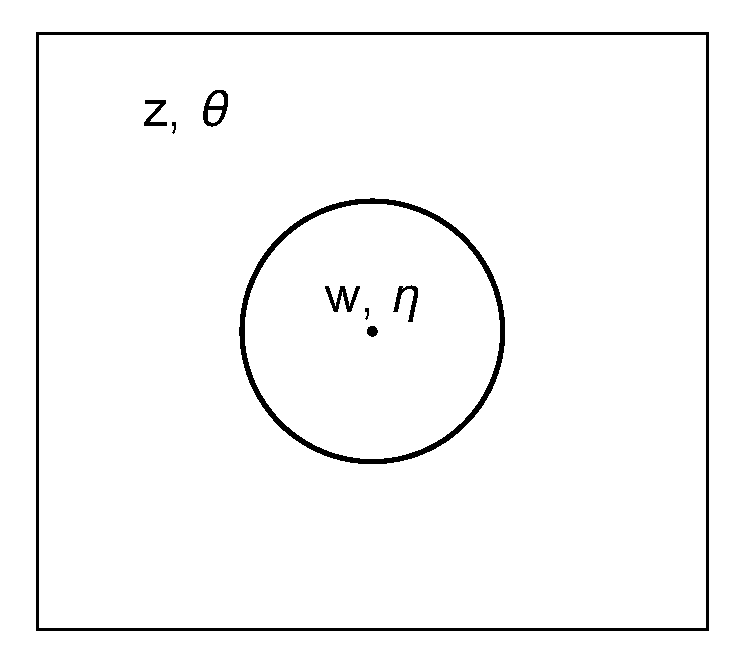
\includegraphics[width=.3\textwidth]{figures/SRSNSpuncture.pdf}
\caption{The superplane with an NS puncture.}\label{fig:SRSNSpuncture}
\end{figure}

Given a super chart ${\cal U}$ with super coordinate $(z,\theta)$ that contains a neighborhood of the puncture, we can describe the puncture by marking the origin of a super disc ${\cal D}$, whose super coordinate $(w,\eta)$ is related to $(z,\theta)$ by the superconformal transition map
\ie\label{nspuncmoduli}
z = w + t + \eta \nu, ~~~~ \theta = \eta + \nu.
\fe
Here $t$ is an even modulus and $\nu$ an odd modulus. Equivalently, we could say that the puncture is ``located at'' $(z, \theta) = (t, \nu)$. Moreover, the punctured SRS should be invariant under a superconformal transformation of $(w,\eta)$ that preserves $(0,0)$. The latter in its infinitesimal form can be expressed as the coordinate variation
\ie\label{delwuv}
\delta w =  v(w) + \eta \zeta(w)  ,~~~~ \delta \eta =  \zeta(w) + \eta \partial v(w) ,
\fe
where $v(w)$ and $\zeta(w)$ are Grassmann-even and odd holomorphic functions in $w$ that vanish at $w=0$. 

Suppose the NS puncture comes with a vertex operator $\Phi$, that is, $\Phi(0)$ is inserted at the origin of the disc ${\cal D}$. According to (\ref{deltsup}), the effect of (\ref{delwuv}) is to change $\Phi(0)$ by
\ie\label{vasupphic}
- \oint {dw d\eta\over 2\pi i} \mathbb{T}(w,\eta) \left[ v(w) + 2 \eta \zeta(w) \right] \Phi(0) = -\oint {dw\over 2\pi i} \left[ v(w)T(w) + \zeta(w) G(w) \right]\Phi(0) ,
\fe
which ought to vanish when $v(0)=\zeta(0)=0$. This is equivalent to the condition that $\Phi$ is a weight zero superconformal primary, namely $L_n|\Phi\rangle = G_{n+{1\over 2}}|\Phi\rangle = 0$ for all $n\geq 0$. On the other hand, an infinitesimal deformation of the moduli $(t, \nu)$ is equivalent to inserting 
\ie\label{deltatsimp}
\delta{\cal T} = \delta t\,  \oint {dw\over 2\pi i} T(w) + \delta\nu\, \oint {dw\over 2\pi i }  [G(w)  - \nu T(w) ]
\fe
into a correlation function.  %on the SRS, where  ${\cal T}_t , {\cal T}_\nu$ are super contour integrals that can be reduced to super-Virasoro generators acting on $\Phi(0)$,
%\ie\label{tnudef}
%& {\cal T}_t = - \oint {dw d\eta\over 2\pi i} \mathbb{T}(w,\eta)  \left.\left[ {\partial w\over \partial t} - {\partial \eta\over \partial t} \eta \right]\right|_{z,\theta} = \oint {dw\over 2\pi i} T(w) = L_{-1},
%\\
%& {\cal T}_\nu = -\oint {dw d\eta\over 2\pi i} \mathbb{T}(w,\eta)  \left.\left[ {\partial w\over \partial \nu} - {\partial \eta\over \partial \nu} \eta \right]\right|_{z,\theta} 
%= \oint {dw\over 2\pi i }  [G(w)  - \nu T(w) ] = G_{-{1\over 2}} - \nu L_{-1} .
%\fe
Exponentiating (\ref{deltatsimp}), we see that turning on the moduli $(t,\nu)$ amounts to replacing $\Phi(0)$ with $\Phi(t,\nu) = (1 + \nu G_{-{1\over 2}}) \Phi(t)$, the latter taking precisely the form of a primary superfield (\ref{chisuperfiel}).



Now we turn to the superstring amplitude (\ref{superamp}), (\ref{omegasupercorr}) in the presence of an NS puncture where a vertex operator ${\cal V}^{(-1)}$, of picture number $-1$, is inserted. We must include the appropriate insertions of ${\cal B}_t$ and $\delta({\cal B}_\nu)$, and integrate with respect to the moduli $(t,\nu)$. The treatment of the even modulus $t$ is identical to that of (\ref{bminusones}), (\ref{intverta}). For the odd modulus $\nu$, using (\ref{btknum}) we can express ${\cal B}_\nu$ as a contour integral either in the $(w,\eta)$ coordinate or equivalently in the $(z,\theta)$ coordinate,
\ie
{\cal B}_\nu &= \oint {dw\over 2\pi i} (2\B^{(w)}(w) - \nu b^{(w)}(w)) = \oint {dz\over 2\pi i} (2\B^{(z)}(z) + \nu b^{(z)}(z)),
\fe 
where the superscripts of $\B$ and $b$ indicate the superconformal frame in which the fields are defined. The integral over $\nu$ then produces a picture number 0 vertex operator
\ie\label{vphipicraise}
{\cal V}^{(0)}(0) &= \int \delta(d\nu) \big( 1+\nu G_{-{1\over 2}} \big)   \delta\big( 2\B_{-{1\over 2}} - \nu b_{-1} \big) {\cal V}^{(-1)}(0) 
\\
&=   \left[ {1\over 2} G_{-{1\over 2}}  \delta( \B_{-{1\over 2}} ) - {1\over 4} b_{-1} \delta'(\B_{-{1\over 2}}) \right]  {\cal V}^{(-1)}(0) .
\fe
Note that the unusual looking operator $\delta(\B_{-{1\over 2}})\equiv \delta(\oint {dw\over 2\pi i} \B(w))$ raises picture number 1 and changes weight by $-{1\over 2}$, and likewise $\delta'(\B_{-{1\over 2}})$ changes weight by $-1$. As in section \ref{sec:physupers}, ${\cal V}^{(-1)}$ may be taken to be the OCQ representative of a physical superstring state, of the form (exhibiting the holomorphic sector only)
\ie\label{ocqrepae}
{\cal V}^{(-1)} = c \delta(\C) V^{\rm m},
\fe
where $V^{\rm m}$ is a weight ${1\over 2}$ matter superconformal primary. 

It is not entirely straightforward to evaluate $\delta(\B_{-{1\over 2}})\delta(\C)$ using the technique introduced in section \ref{sec:ghostpicture}. We begin by observing that $\delta(\B_{-{1\over 2}})\delta(\C)$ has vanishing weight, picture number, as well as $\B\C$ ghost number. The only such operator in the $\B\C$ system is proportional to the identity. To fix its normalization, let us compare with
\ie\label{limwbcg}
\lim_{w\to 0} {1\over w}\delta(\B(w)) \delta(\C(0)) = \lim_{w\to 0} {1\over w} e^{\phi(w)} e^{-\phi(0)} =1.
\fe
When inserted into the $\B\C$ system path integral, $\delta(\C(0))$ creates an extra zero mode of the $\B$ ghost, of the form $\B(w)\sim a\, w^{-1}$ near $w=0$. Upon integration over $a$, we learn that the correlation function of $\delta(\B_{-{1\over 2}})\delta(\C(0))$ agrees with that of $\lim_{w\to 0} {1\over w}\delta(\B(w)) \delta(\C(0))$, thereby determining
\ie\label{bctrickone}
\delta(\B_{-{1\over 2}}) \delta(\C) = 1.
\fe
By a similar calculation, $\delta'(\B_{-{1\over 2}}) \delta(\C)$ has weight $-{1\over 2}$, picture number 0, and $\B\C$ ghost number 1, and is found to be
\ie\label{bctricktwo}
\delta'(\B_{-{1\over 2}}) \delta(\C) = \C.
\fe
Using (\ref{bctrickone}) and (\ref{bctricktwo}), we can now evaluate (\ref{vphipicraise}) to give
\ie\label{vzeropicrais}
{\cal V}^{(0)} &=  - {1\over 2} G_{-{1\over 2}} c V^{\rm m} + {1\over 4} \C V^{\rm m}
={1\over 2} c G_{-{1\over 2}}^{\rm m} V^{\rm m} - {1\over 4} \C V^{\rm m}.
\fe
In conclusion, the $(-1)$-picture vertex operator ${\cal V}^{-1}$ of the OCQ form (\ref{ocqrepae}) inserted at an NS puncture of the SRS is equivalent to the 0-picture vertex operator ${\cal V}^0$ (\ref{vzeropicrais}) after integrating out the odd moduli associated with the NS puncture (thus converting it to an ``ordinary'' puncture on the Riemann surface).




\subsubsection{R punctures}


A Ramond sector vertex operator creates a puncture around which the worldsheet spinor fields are anti-periodic. An ``R puncture" on a SRS is described by marking the origin of a superdisc ${\cal D}$, whose super coordinate system $(w, \eta)$ has the property that $\eta$ is anti-periodic around $w=0$.\footnote{If one insists on using single-valued coordinates, one may cover the neighborhood of the R puncture with an upper half disc ${\cal D}_\cap$ parameterized by $(w, \eta)$ with ${\rm Im} (w)\geq 0$, and a lower half disc ${\cal D}_\cup$ parameterized by $(w, \eta')$ with ${\rm Im}( w)\leq 0$, such that the transition maps are $\eta=\eta'$ along $w\in \mathbb{R}_-$, and $\eta=-\eta'$ along $w\in \mathbb{R}_+$.} 
The punctured SRS should be invariant under a superconformal transformation of $(w,\eta)$ that respects the anti-periodicity of $\eta$ and preserves $(0,0)$, i.e. of the form (\ref{delwuv}) where $v(w)$ and $\zeta(w)$ take the form
\ie\label{vgramon}
v(w) = \sum_{n=0}^\infty a_n w^{n+1},~~~~\zeta(w) = \sum_{n=0}^\infty \zeta_n w^{n+{1\over 2}}.
\fe
Suppose the R puncture comes with the insertion of a Ramond vertex operator $S(0)$. The vanishing of (\ref{vasupphic}) with  $\Phi$ replaced by $S$ now amounts to $L_n|S\rangle = G_n|S\rangle=0$, for all $n\geq 0$, in agreement with the Ramond sector OCQ representative (\ref{vrsuperocq}).

\begin{figure}[h!]
\centering
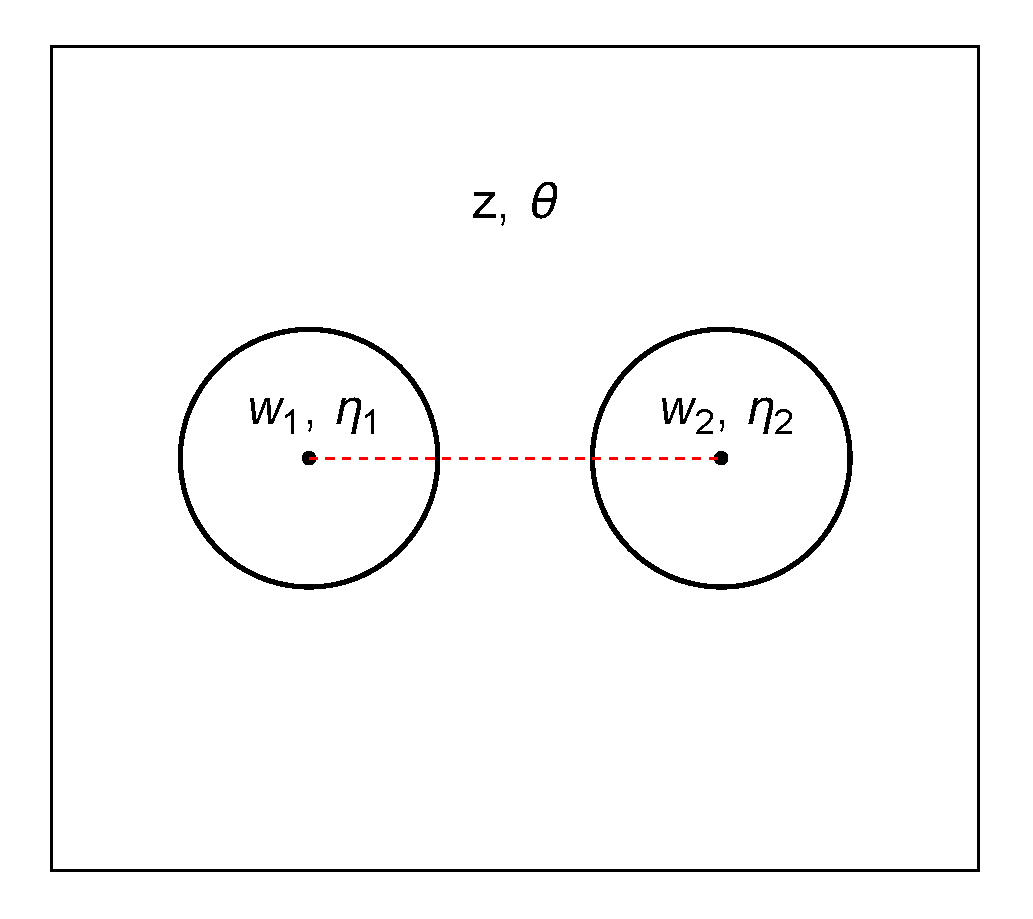
\includegraphics[width=.4\textwidth]{figures/SRSRpair.pdf}
\caption{The superplane with a pair of R punctures.}\label{fig:SRSRpair}
\end{figure}

Evidently, the R punctures must come in pairs. Consider, as an example, the super plane with a pair of R punctures, which may be covered by a super chart ${\cal U}$ parameterized by $(z, \theta)$, and a pair of discs ${\cal D}_1, {\cal D}_2$ each containing an R puncture at the origin of their super coordinates $(w_i, \eta_i)$, $i=1,2$, with the transition maps
\ie\label{simprpunctrans}
w_i = z - t_i, ~~~~ \eta_i = \theta.
\fe
As $\eta_i$ is anti-periodic around $w_i=0$, we must also require $\theta$ to undergo a monodromy $\theta\to -\theta$ as $z$ circles around either $t_1$ or $t_2$. Potential odd moduli arise from the deformation of (\ref{simprpunctrans}) to the more general transition maps
\ie\label{zeptrans}
w_i = z - t_i + \theta g_i(z) , ~~~ \eta_i =\theta + g_i(z),
\fe
where $g_i(z)= \sum_{n\in\mathbb{Z}} g_{i,n} (z-t_i)^{n-{1\over 2}}$ with Grassmann-odd coefficients $g_{i,n}$. We can use coordinate transformations on $(w_i, \eta_i)$ of the form (\ref{delwuv}) with (\ref{vgramon}) to shift $g_{i,n}$ independently for all $n\geq 1$, and use a coordinate transformation $(z,\theta) \to (z', \theta')$ on ${\cal U}$ of the form
\ie\label{zthegz}
& z' = z + \theta \kappa(z),~~~ \theta' = \theta + \kappa(z),
\fe
where $\kappa(z)$ vanishes at infinity and has square root branch points at $z=t_1, t_2$, to eliminate $g_{i,n}$ for all $n\leq -1$, as well as shifting $g_{1,0}$ and $g_{2,0}$ simultaneously with
\ie\label{ramooddtransmap}
\kappa(z) = {\epsilon \over \sqrt{(z-t_1)(z-t_2)}}.
\fe
This leaves one independent odd variable, say either $g_{1,0}$ or $g_{2,0}$, as the only odd modulus. We conclude that a pair of R punctures introduce 2 even moduli and 1 odd modulus.






\subsection{The supermoduli space}
\label{sec:supermodulispace}



\subsubsection{Odd moduli}
\label{sec:oddmoduli}

An infinitesimal moduli deformation of an ordinary Riemann surface $\Sigma$ is in 1-1 correspondence with a zero mode of the $b$ ghost, i.e. a holomorphic quadratic differential. Similarly, an infinitesimal odd moduli deformation of a split SRS $\mathfrak{C}_0$ is in 1-1 correspondence with a zero mode of the $\B$ ghost subject to the spins structure. In the absence of punctures, the difference between the number of $\B$ zero modes (or odd moduli) and the number of $\C$ zero modes (or superconformal Killing spinors) can be determined from the anomaly of the $\B\C$ ghost number (\ref{betagamsym}) to be equal to $2h-2$, where $h$ is the genus of the surface, regardless of the spin structure. As we have seen in the previous section, each NS puncture introduces one additional odd modulus, and each pair of R punctures introduce one additional odd modulus. In the case of genus $h=0$ with at least 3 punctures, $h=1$ with at least 1 puncture, or $h\geq 2$ with any number of punctures, there are no superconformal Killing spinors (as they would square to conformal Killing vectors), and therefore the number of odd moduli $d_o$ is equal to the $\B\C$ ghost number anomaly
\ie\label{doddcount}
d_o = 2h -2 + n_{\rm NS} + {n_{\rm R} \over 2},
\fe
where $n_{\rm NS}$ and $n_{\rm R}$ are the number of NS and R punctures respectively. This conclusion holds for non-split punctured SRS as well.

A particularly useful parameterization of the odd moduli of a SRS can be made as follows. Starting with the split SRS $\mathfrak{C}_0$, we choose a set of points $z_a$ on the underlying Riemann surface $\Sigma$, $a=1,\cdots, d_o$, and the charts $U_a= D_a\cup U_a'$, where $D_a$ is a sufficiently small disc that contains $z_a$ and $U_a'$ is an annulus that contains $\partial D_a$ but not $z_a$. We can further promote $D_a$ and $U_a'$ to super charts ${\cal D}_a$ and ${\cal U}_a'$, whose coordinates $(w, \eta)$ and $(z,\theta)$ are simply related by
\ie
w=z-z_a,~~~~ \eta=\theta.
\fe
A new SRS $\mathfrak{C}_\nu$ is constructed by deforming the transition map between ${\cal D}_a$ and ${\cal U}_a'$ on their overlap to
\ie\label{discgluingoddmod}
w=z-z_a - {\theta\nu^a\over z-z_a} ,~~~~ \eta=\theta - {\nu^a\over z-z_a}.
\fe
$(\nu^1,\cdots,\nu^{d_o})$ can be viewed as fermionic coordinates on a chart $\mathfrak{U}_{\{z_a\}}$ of the supermoduli space $\mathfrak{M}_{h,n,\epsilon}$, with the points $\{z_a\}$ chosen on $\Sigma$ over a chart of the bosonic moduli space.\footnote{$\{z_a\}$ must be chosen so as to avoid possible degeneration of the $\nu^a$ coordinates, whose occurrence will be analyzed in section \ref{sec:pcocoordinates}.} According to (\ref{deltsup}), turning on the odd moduli $\nu^a$ is equivalent to deforming the SCFT on $\mathfrak{C}_0$ by inserting
\ie\label{prodgdef}
\prod_{a=1}^{d_o} \left[ 1 - \oint_{\partial D_a} {dw\over 2\pi i} G^{(w)}(w) {\nu^a\over w} \right] = \prod_{a=1}^{d_o} \left[ 1+\nu^a G^{(z)}(z_a) \right],
\fe
where $G^{(z)}(z_a)$ on the RHS is understood as defined in the $z$-coordinate on the chart $U_a$.

Given a generic set of $k$ points $\{u_i\}$ and $2g-1+k$ points $\{ v_j \}$ on $\Sigma$, there is up to constant rescaling a unique weight $-{1\over 2}$ meromorphic differential $f(z) (dz)^{-{1\over 2}}$ subject to the spin structure of $\mathfrak{C}_0$, with simple zeroes at $u_i$ and simple poles at $v_j$, given in terms of the correlator of $\B\C$ system via
\ie\label{fkconstr}
f(z) = {1\over \left\langle \delta(\C(z)) \prod_{i=1}^k \delta(\C(u_i)) \prod_{j=1}^{2g-1+k} \delta(\B(v_j)) \right\rangle_{\mathfrak{C}_0}}.
\fe
For simplicity let us assume that there are only NS punctures on the SRS. Using $f(z)$ constructed as (\ref{fkconstr}) in the $k=n_{\rm NS}$ case ($d_o = 2g-2+k$), setting $v_a=z_a$, $a=1,\cdots, d_o$, $v_{d_o+1}\equiv z_1'$, and $u_1,\cdots, u_k$ to the locations of the punctures, and further normalizing ${\rm Res}_{z\to z_1} f(z) = 1$, we can write
\ie
G(z_1) = \oint_{C_{z_1}} {dz\over 2\pi i} f(z) G(z),
\fe
where $C_{z_1}$ is a small counterclockwise contour encircling $z_1$, and rewrite (\ref{prodgdef}) as
\ie\label{gcontdefprod}
& \left[ 1+\nu^1 \oint_{C_{z_1}} {dz\over 2\pi i} f(z) G(z) \right] \prod_{a=2}^{d_o} \left[ 1+\nu^a G(z_a) \right]
\\
& = \left[ 1 - \nu^1 f^{(-1)}(z_1') G(z_1') - \nu^1 \sum_{b=2}^{d_o} \oint_{C_{z_b}} {dz\over 2\pi i} f(z) G(z) \right] \prod_{a=2}^{d_o} \left[ 1+\nu^a G(z_a) \right]
\\
&= \left[ 1 - \nu^1 f^{(-1)}(z_1') G(z_1') \right] \prod_{a=2}^{d_o} \left[ 1+\nu^a G(z_a) \right] G(z_1') 
\\
&~~~~ - \nu^1 \sum_{b=2}^{d_o} \left[ f^{(-1)}(z_b) G(z_b) - 2\nu^b f^{(0)}(z_b) T(z_b) \right] \prod_{a=2,a\not=b}^{d_o} \left[ 1+\nu^a G(z_a) \right].
\fe
Here $f^{(n)}(z_b)$ stands for the coefficient of $(z-z_b)^n$ in the Laurent series of $f(z)$ around $z=z_b$. The first equality of (\ref{gcontdefprod}) follows from deforming the contour $C_{z_1}$ to $-\sum_{b=2}^{d_o} C_{z_b}$, picking up a residue at $z=z_1'$ where $f(z)$ has a pole, but freely past all NS punctures where $f(z)$ has a zero. The second equality of (\ref{gcontdefprod}) follows from the OPE $G(z) G(0) \sim {2\over z} T(0)$ and the absence of order $z^0$ term thereof. The RHS of (\ref{gcontdefprod}) can be put back in a product form
\ie\label{taprodcagg}
\left[ 1 + \nu'^1 f^{(-1)}(z_1') G(z_1') \right] \prod_{a=2}^{d_o} \left[ 1+\nu'^a G(z_a) \right] \left[ 1 + \sum_{b=2}^{d_o} 2\nu^1\nu^b f^{(0)}(z_b) T(z_b) \right],
\fe
where $\nu'^a$ are related to $\nu^a$ by
\ie{}
& \nu'^1 = -\nu^1 f^{(-1)}(z_1'),
\\
& \nu'^a = \nu^a - \nu^1 f^{(-1)}(z_a),~~~ a=2,\cdots, d_o.
\fe
The last factor in (\ref{taprodcagg}) represents an infinitesimal deformation of the even moduli $t^k \to t'^k = t^k + \delta t^k$ (where $\delta t^k$ is a linear combination of $\nu^1\nu^b$), and the equivalence between (\ref{prodgdef}) and (\ref{taprodcagg}) represents a transition map $(t^k, \nu^a) \mapsto (t'^k, \nu'^a)$ between the coordinate charts $\mathfrak{U}_{\{z_1,\cdots, z_{d_o}\}}$ and $\mathfrak{U}_{\{z_1',z_2,\cdots, z_{d_o}\}}$ of the supermoduli space $\mathfrak{M}_{h, n, \epsilon}$.


\subsubsection{Integration}
\label{sec:supermodinte}

The notion of integral over the supermoduli space, or more precisely over the super contour $\mathfrak{G}_{h,n,\epsilon}$ in (\ref{superamp}), requires explanation as the superspaces in question do not necessarily admit global fermionic coordinates and one cannot naively apply the Grassmann/Berezin rule of integration.

To begin with, consider a supermanifold $\mathfrak{M}$ of dimension $n_e|n_o$ covered by super charts $\mathfrak{U}_\A$ along with the coordinate maps\footnote{We denote by $\mathbb{R}^{p|*q}$ the vector superspace parameterized by $p$ real bosonic coordinates and $q$ fermionic coordinates, emphasizing that there is no reality condition involving the fermionic coordinates.}
\ie
\varphi_\A: \mathtt{U}_\A\times \mathbb{R}^{0|*n_o}\to \mathfrak{U}_\A,
\fe
where $\mathtt{U}_\A$ are bosonic charts that cover the reduced space, an $n_e$-dimensional manifold ${\cal M}$. We denote by $\pi_\A: \mathfrak{U}_\A\to \mathtt{U}_\A$ the corresponding projection map, i.e. $\pi_\A\circ \varphi_\A$ simply forgets the fermionic coordinates. Starting with a partition of unity on ${\cal M}$, that is a collection of smooth non-negative functions $f_\A$ with support in $\mathtt{U}_\A$ and
\ie
\sum_\A f_\A = 1, 
\fe
we can construct a partition of unity on $\mathfrak{M}$ with
\ie\label{faparti}
F_\A = {\pi_\A^* f_\A \over \sum_\B \pi_\B^* f_\B},~~~~ \sum_\A F_\A = 1.
\fe
Note that the ``fermionic fibers'' of the projection $\pi_\A$ and $\pi_\B$ over the two charts $\mathtt{U}_\A$ and $\mathtt{U}_\B$ generally do not agree on their overlap $\mathtt{U}_\A\cap \mathtt{U}_\B$. Nonetheless, $\sum_\B \pi_\B^* f_\B$ is equal to 1 plus quadratic and higher order terms in the fermionic coordinates, and is therefore invertible, ensuring that $F_\A$ in (\ref{faparti}) is well-defined. The integration of a super form $\Omega$ over $\mathfrak{M}$ can now be defined via the partition of unity as
\ie\label{momintegral}
\int_{\mathfrak M} \Omega = \sum_\A \int_{\mathtt{U}_\A\times \mathbb{R}^{0|*n_o}} \varphi_\A^*(F_\A\, \Omega),
\fe
where each summand on the RHS is defined as the usual Grassmann integral. One can show that the result of the integration does not depend on the choice of super charts $\mathfrak{U}_\A$ nor the choice of partition of unity, and obeys the supermanifold version of Stokes' theorem.\footnote{For further details see Witten, {\it Notes On Supermanifolds and Integration}, Pure Appl. Math. Quart. \textbf{15} (2019) no.1.} 




It is important to note that to define the pullback of an integral form $\mathfrak f^*\omega$ a priori requires the map $\mathfrak f$ to have non-singular Berezinian. Consider for instance the top form
\ie
\omega = \prod_{i=1}^{n_e} dt^i \prod_{a=1}^{n_o} \delta(d\nu^a)
\fe
on $\mathbb{R}^{n_e|*n_o}$ parameterized by even coordinates $t^i$ and odd coordinates $\nu^a$. The pullback of $\omega$ with respect to the map $\mathfrak{f}:(t^i,\nu^a)\mapsto (f^i(t,\nu), g^a(t,\nu))$ is evaluated as
\ie
\mathfrak{f}^*\omega = {\rm Ber}(\mathfrak{f}) \, \omega,
\fe
where the Berezinian ${\rm Ber}(\mathfrak{f})$ is given by
\ie\label{berezianform}
{\rm Ber}(\mathfrak{f}) ={\det (A - B D^{-1} C)\over \det (D)},~~~~~ {\rm where}~\begin{pmatrix} A^i{}_j & B^i{}_a \\ C^a{}_i & D^a{}_b \end{pmatrix} = \begin{pmatrix} {\partial f^i\over \partial t^j}&{\partial f^i\over \partial \nu^a}  \\ {\partial g^a\over \partial t^i} & {\partial g^a\over \partial \nu^b} \end{pmatrix}.
\fe
In particular, the Berezinian is non-singular only if the matrix $D = \left({\partial g^a\over \partial\nu^b}\right)$ is non-degenerate.

The integral (\ref{momintegral}) can be equivalently computed by viewing $\mathfrak{M}$ as a top-dimensional integration contour formed by gluing together segments, each of which is parameterized with a non-degenerate coordinate system, as follows. Consider a cell decomposition of the reduced space ${\cal M} = \bigsqcup_\A \mathtt{D}_\A$, say a dual triangulation, with $\mathtt{D}_\A\subset \mathtt{U}_\A$. The integral of $\Omega$ over the uplifted patch $\pi_\A^{-1}(\mathtt{D}_\A)$ can be evaluated as the Grassmann integral $\int_{\mathtt{D}_\A\times \mathbb{R}^{0|*n_o}} \varphi_\A^*\Omega$. The sum of the patches does not reproduce $\mathfrak{M}$, however, as the fibers of $\pi_\A^{-1}$ and $\pi_\B^{-1}$ generally do not agree along the codimension 1 face $\mathtt{D}_{\A\B} = \mathtt{D}_\A\cap \mathtt{D}_\B$ between neighboring cells $\mathtt{D}_\A, \mathtt{D}_\B$. We must therefore add the integral over $\Omega$ over an interpolating patch, defined by
\ie\label{codimoneint}
\varphi_{\A\B}: ~[0,1] \times \mathtt{D}_{\A\B} \times \mathbb{R}^{0|*n_o} \to \mathfrak{U}_\A \cap \mathfrak{U}_\B,
\fe
such that $\varphi_{\A\B}(\{0\}\times\mathtt{D}_{\A\B}\times \mathbb{R}^{0|*n_o})$ agrees with $\pi_\A^{-1}(\mathtt{D}_{\A\B})$, and that $\varphi_{\A\B}(\{1\}\times \mathtt{D}_{\A\B}\times \mathbb{R}^{0|*n_o})$ agrees with $\pi_\B^{-1}(\mathtt{D}_{\A\B})$, for every face $\mathtt{D}_{\A\B}$. This still leaves gaps over the codimension 2 loci $\mathtt{D}_{\A\B\C}=\mathtt{D}_\A\cap \mathtt{D}_\B\cap \mathtt{D}_\C$, and we must add the integral over an interpolating patch defined by a map $\varphi_{\A\B\C}: \Delta^2 \times \mathtt{D}_{\A\B\C} \times \mathbb{R}^{0|*n_o} \to \mathfrak{U}_\A \cap \mathfrak{U}_\B\cap \mathfrak{U}_\C$, where $\Delta^2$ is a 2-simplex, and so forth. Eventually the sum of integrals over $\pi_\A^{-1}(\mathtt{D}_\A)$ together with interpolating patches $\varphi_{\A\B}, \varphi_{\A\B\C},\cdots$ of all codimensions reproduces the integral over $\mathfrak M$.


\begin{figure}[h!]
\centering
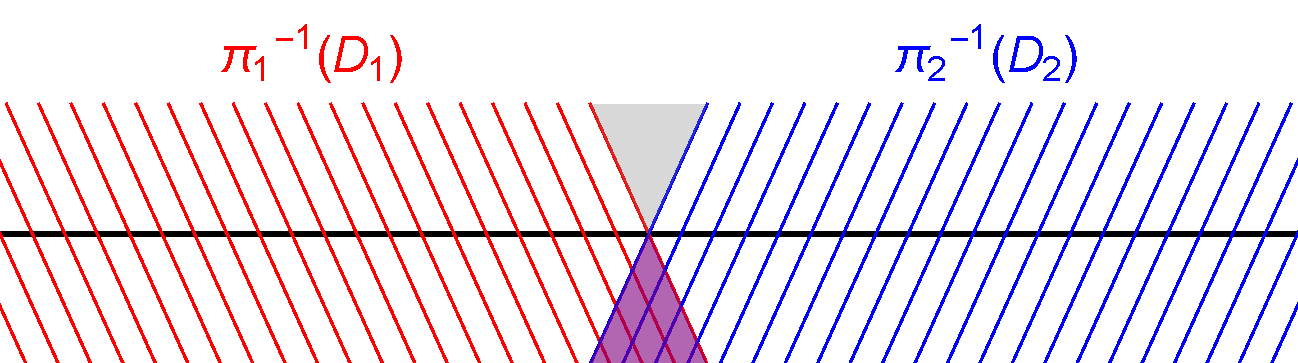
\includegraphics[width=.6\textwidth]{figures/interpatch.pdf}
\caption{The uplifted patches $\pi_1^{-1}(D_1)$ and $\pi_2^{-1}(D_2)$ generally do not agree along $D_1\cap D_2$. The integrals along the fibers of $\pi_1$ and $\pi_2$ must be supplemented by the integration over the interpolating patch, shown in gray (with positive orientation) and purple (with negative orientation).}\label{fig:interpatch}
\end{figure}


%Let $(t^k, \nu^a)$ be the bosonic and fermionic coordinates on $\mathbb{R}^{n_e|*n_o}$. Under a change of variable $(t, \nu)\to (t', \nu')$, the integral form $\prod_{k=1}^{n_e} dt^k \prod_{a=1}^{n_o} \delta(d\nu^a)$ transforms by the Berezinian...

As seen in section \ref{sec:oddmoduli}, the supermoduli space $\mathfrak{M}_{h,n,\epsilon_L}$ can be covered with a collection of super charts of the form $\mathfrak{U}_\A = \mathfrak{U}_{\{z_a^{(\A)}\}}$, where $\{z_a^{(\A)}\}$ is a set of $d_o$ points suitably chosen on $\Sigma$ over a chart ${\mathtt{U}}_\A$ of the bosonic moduli space ${\cal M}_{h,n}$. %\footnote{We will see in section \ref{sec:pcocoordinates} that $\{z_a^{(\A)}\}$ are precisely the locations where the picture changing operators are inserted.} 
We will denote by $\varphi_\A$ the coordinate map $\mathtt{U}_\A\times \mathbb{R}^{0|*d_o}\to \mathfrak{U}_\A$ and $\pi_\A$ the projection map $\mathfrak{U}_\A\to \mathtt{U}_\A$. Analogously we write $\overline\varphi_\A$ and $\overline\pi_\A$ for the coordinate and projection maps associated with super charts $\overline{\mathfrak U}_\A$ of the supermoduli space $\overline{\mathfrak{M}_{h,n,\epsilon_R}}$ associated with the anti-holomorphic sector. 

The integration contour $\mathfrak{G}_{h,n,\epsilon}\subset \mathfrak{M}_{h,n,\epsilon_L}\times \overline{\mathfrak{M}_{h,n,\epsilon_R}}$ in the prescription for the superstring amplitude (\ref{superamp}) is a codimension $d_e|0$ subspace whose reduced space is the diagonal subspace of ${\cal M}_{h,n}\times \overline{{\cal M}_{h,n}}$. One may construct such a contour starting with a cell decomposition of the bosonic moduli space ${\cal M}_{h, n}=\bigsqcup_\A\mathtt{D}_\A$, with $\mathtt{D}_\A\subset \mathtt{U}_\A$, and consider the sum of the uplifted patches $(\pi_\A^{-1}\times \overline\pi_\A^{-1})(\mathtt{D}_\A)$ in $\mathfrak{M}_{h,n,\epsilon_L}\times \overline{\mathfrak{M}_{h,n,\epsilon_R}}$. However, along the codimension 1 faces between neighboring cells $\mathtt{D}_{\A\B}=\mathtt{D}_\A\cap\mathtt{D}_\B$, the fibers of $\pi_\A^{-1}\times \overline\pi_\A^{-1}$ and $\pi_\B^{-1}\times \overline\pi_\B^{-1}$ generally do not agree. To form a closed contour $\mathfrak{G}_{h,n,\epsilon}$, as would be necessary for the BRST invariance of the superstring amplitude, one must add additional interpolating patches along the lines of (\ref{codimoneint}) and its higher codimension analogs. Such a procedure, known as ``vertical integration'', will be described in more detail in section \ref{sec:verticalpco}.


\subsection{Unitarity of superstring amplitudes}
\label{sec:unitarysuper}

Similarly to the bosonic string consideration of section \ref{sec:factortube}, the superstring amplitude (\ref{superamp}) is subject to highly nontrivial consistency conditions imposed by the unitarity of the S-matrix in 10-dimensional Minkowskian spacetime. In particular, integration near the boundary of the moduli space gives rise to singularities of the (analytically continued) scattering amplitude that correspond to the propagation of intermediate on-shell particles.

Near the degeneration limit where the worldsheet surfaces $\Sigma$ pinches into surfaces $\Sigma_1$ and $\Sigma_2$ joined at a puncture, the geometry of the SRS $\mathfrak{C}$ can be constructed via the plumbing fixture. We begin with the case of a pair of NS punctures, located at super coordinate $(z,\theta)=(0,0)$ on a disc ${\cal D}_1$ in the SRS $\mathfrak{C}_1$, and at $(z',\theta')=(0,0)$ on a disc ${\cal D}_2$ in the SRS $\mathfrak{C}_2$. The plumbing fixture reduces the total number of NS punctures by 2, and according to (\ref{doddcount}) leaves the total number of odd moduli unchanged. It suffices to consider the plumbing map
\ie\label{supplumb}
z' = {q\over z},~~~~ \theta' = \pm i {\sqrt{q}\over z}\theta,
\fe
where $q=e^{2\pi i \tau}$ with ${\rm Im}(\tau)>0$. The choice of sign in the map between the fermionic coordinates is inessential here as it can be undone by flipping the signs of all fermionic coordinates on either $\mathfrak{C}_1$ or $\mathfrak{C}_2$. The plumbing fixture introduces an even modulus $\tau$ that comes with the insertion of
\ie\label{btauns}
& {\cal B}_\tau = \oint {dz d\theta \over 2\pi i} \mathbb{B}(z, \theta) \left.\left[ {\partial z\over \partial\tau} - {\partial \theta\over\partial\tau} \theta \right]\right|_{z',\theta'} = \oint {dz d\theta \over 2\pi i} \mathbb{B}(z, \theta) 2\pi i z 
= 2\pi i b_0.
\fe
If the punctures are also of NS type in the anti-holomorphic sector, then the contribution to the amplitude (\ref{superamp}) from near the degeneration limit $q\to 0$ is given by 
\ie\label{ampnearxxbsuper}
& \mathfrak{N}_{h,n} \int_{{\rm Im}(\tau)>0} d\tau \wedge d\bar\tau \, \langle\langle S_2 |{\cal B}_{\bar\tau} {\cal B}_\tau\, q^{L_0} \bar q^{\widetilde L_0} | S_1 \rangle ,
\fe
where the surface states $|S_i\rangle$ are produced by the matter+ghost SCFT on ${\mathfrak C}_i\backslash {\cal D}_i$, integrated over their respective supermoduli and summed over their respective spin structures, generalizing those of (\ref{ampnearxxb}) in the bosonic string case. An analysis similar to that of section \ref{sec:factorbos} shows that (\ref{ampnearxxbsuper}) produces precisely the poles of the superstring amplitude due to the propagation of an intermediate on-shell particle, in correspondence with states in the (NS,NS) sector that are $Q_B$-closed, annihilated by $b_0, \widetilde b_0, L_0, \widetilde L_0$, and satisfy the GSO projection condition $(-)^F=(-)^{\widetilde F}=1$ (as do the surface states $|S_1\rangle$ and $|S_2\rangle$). This also determines, similarly to (\ref{nexpresa}), a relation on the normalization factors\footnote{We adopt the same normalization of the superstring vertex operators as in (\ref{vvnormvonv}) with $K_{S^2}={8\pi\over \A'}$.}
\ie\label{factofrakn}
{\mathfrak N}_{g_1, n_1} {\mathfrak N}_{g_2, n_2}  = - i {\mathfrak N}_{g_1+g_2, n_1+n_2-2}.
\fe

In the degeneration limit where a handle of $\Sigma$, subject to (NS,NS) periodicity condition, pinches, we have contributions from the plumbing fixture joining a pair of discs on the same surface, in the form (\ref{supplumb}) except that now the two possible signs in the transition map correspond to two different spin structures on $\Sigma$ in the holomorphic sector. The sum over the two spin structures imposes chiral GSO projection on the state propagating through the plumbing fixture, while giving an overall factor of 2. Likewise, we also have two different spin structures in the anti-holomorphic sector that arise from the plumbing fixture. This leads to the normalization condition
\ie\label{loopfrakn}
{\mathfrak N}_{h-1, n+2} = - 4 i {\mathfrak N}_{h, n}.
\fe
(\ref{factofrakn}) and (\ref{loopfrakn}) together determine
\ie\label{nhmsuperss}
{\mathfrak N}_{h,n} = { i^{3h-3+n} \over 2^{2h}},
\fe
up to a factor that can be absorbed into a constant shift of the dilaton.

Next we turn to the degeneration limit that involves a pair of R punctures, located at $(z,\theta)=(0,0)$ on a disc ${\cal D}_1$ and at $(z',\theta')=(0,0)$ on a disc ${\cal D}_2$. The plumbing fixture reduces the total number of R punctures by 2, and therefore increases the total number of odd moduli by 1. The relevant plumbing map is
\ie\label{ramondplumb}
z = q z'^{-1} \pm i  \theta' \nu q^{1\over 2} z'^{-{3\over 2}}  , ~~~ \theta = \pm i \theta' q^{1\over 2}  z'^{-1} + \nu z'^{-{1\over 2}} .
\fe
The even modulus $\tau$ and odd modulus $\nu$ come with the insertion of ${\cal B}_\tau  \delta({\cal B}_\nu)$ in the superstring amplitude, where
\ie\label{bbrplumb}
& {\cal B}_\tau = \oint {dz d\theta\over 2\pi i} \mathbb{B}(z, \theta) 2\pi i \left( z -  \theta \nu q^{-{1\over 2}} z^{1\over 2} \right) = 2\pi i (b_0 - \nu q^{-{1\over 2}} \B_0),
\\
& {\cal B}_\nu = \oint {dz d\theta\over 2\pi i} \mathbb{B}(z, \theta) \left( - 2 \theta q^{-{1\over 2}} z^{1\over 2} +  \nu q^{-1} z \right) = -2 q^{-{1\over 2}} \B_0 - q^{-1} \nu b_0.
\fe
Turning on the odd modulus $\nu$ itself amounts to inserting $1+\delta{\cal T}$, where (from (\ref{deltsup}))
\ie\label{tacontr}
\delta{\cal T} = - \oint {dz d\theta\over 2\pi i} \mathbb{T}(z,\theta) 2\theta \nu q^{-{1\over 2}} z^{1\over 2} = - \nu q^{-{1\over 2}} G_0.
\fe
Note that the contour appearing in (\ref{tacontr}) is understood to enclose that of ${\cal B}_\nu$ in (\ref{bbrplumb}) in the $(z,\theta)$ coordinate. The integral over $\nu$ then produces
\ie\label{holrproj}
\int \delta(d\nu) (1+\delta{\cal T}) \delta({\cal B}_\nu)  {\cal B}_\tau = -{1\over 2} G_0 \delta(\B_0) \cdot 2\pi i b_0,
\fe
acting on the surface state $|S_1\rangle$ that carries picture number $-{3\over 2}$. The operator $\delta(\B_0)$ commutes with $\B_n$ for all $n$ and commutes with $\C_n$ for all $n\not=0$. It acts on the $\B\C$ system oscillator ground states in the $-{3\over 2}$ picture by
\ie\label{delbetzrer}
\delta(\B_0) \left|-\tfrac{3}{2}\right\rangle = |-\tfrac{1}{2}\rangle,~~~~{\rm and}~~ \delta(\B_0) \B_0^n \left|-\tfrac{3}{2}\right\rangle = 0,~~n\geq 1.
\fe
Therefore, (\ref{holrproj}) acting on $|S_1\rangle$ produces a state of picture number $-{1\over 2}$ and obeys Siegel constraint (\ref{betasiegel}), giving rise to 1-particle poles corresponding to physical states in the holomorphic Ramond sector. The anti-holomorphic Ramond sector can be treated similarly.

Finally, let us note that the type IIA and IIB GSO projections are distinguished by the overall sign of the odd spin structure contribution in (\ref{superamp}).




\subsection{The picture changing operator formalism}
\label{pcosec}

Rather than setting the gravitino $\chi_{a\A}$ to zero patch by patch on the worldsheet surface $\Sigma$, which leads to the SRS formulation of the superstring amplitude in section \ref{srssec}, we now return to the global gauge condition (\ref{gchiex}) and consider a specific choice of the fiducial gravitino field where each $\varpi_{m,a\A}(t)$ is a delta function supported at one point on $\Sigma$. Namely, we set $\chi_{a\A} = \hat\chi_{a\A}(t,\nu)$ with
\ie
\hat\chi_{\bar z}{}^+(z,\bar z) = 2\pi \sum_{a=1}^{d_o} \nu^a \delta^2(z-z_a(t)),~~~ \hat\chi_{z}{}^-(z,\bar z) = 2\pi \sum_{a=1}^{\widetilde d_o} \widetilde\nu^a \delta^2(z- \widetilde z_a(t)),
\fe
where the set of points $\{z_a(t)\}$ and $\{\widetilde z_a(t)\}$ are suitably chosen as functions of the even moduli $t$. In the superstring amplitude (\ref{superampprescnl}), ${\cal B}_{\nu^m}$ (\ref{oddmeasurefactor}) and ${\cal G}_{\nu^m}$ (\ref{gnuma}) simplify to
\ie\label{totaloddmeas}
& {\cal B}_{\nu^a} = \B(z_a),~~~~~ {\cal B}_{\widetilde\nu^a} = \widetilde\B(\bar{\widetilde z}_a),
\\
& {\cal G}_{\nu^a} = {1\over 2} G(z_a) + \partial \B(z_a) \sum_k {\partial z_a\over \partial t^k} dt^k,
~~~~ {\cal G}_{\widetilde\nu^a} = {1\over 2}\widetilde G(\bar{\widetilde z}_a) + \bar\partial \widetilde\B(\bar{\widetilde z}_a) \sum_k {\partial \bar{\widetilde z}_a\over \partial t^k} dt^k,
\fe
A priori, the product operator $ {\cal G}_{\nu^a}\delta({\cal B}_{\nu^a})$ appearing in (\ref{superampprescnl}) is singular due to the OPE between $\delta(\B(z_a))$ and the ghost part of the supercurrent $G(z_a)$, and must be regularized. A BRST-invariant regularization of the product ${1\over 2} G(z_a)\delta(\B(z_a))$ gives the {\it picture changing operator} (PCO) ${\cal X}(z_a)$, defined as
\ie\label{pcoregdef}
{\cal X}(z) &= -Q_B\cdot \Theta(\B(z)) = {1\over 2} \lim_{w\to z} \left[ G(w) \delta(\B(z)) - {1\over w-z} b(z) \delta'(\B(z)) \right] - {1\over 4} \partial b(z) \delta'(\B(z)),
\fe
where $\Theta(\B)$ is the ``Heaviside step'' analytic distribution defined by $\Theta'(\B) = \delta(\B)$. This precise expression will be recovered from the SRS formalism in section \ref{sec:pcocoordinates}. In terms of the $(\phi, \eta, \xi)$ representation of the $\B\C$ system, in addition to (\ref{bcdict}), we can identify
\ie\label{thetabetadic}
\Theta(\B) \simeq -\xi, ~~~~ \delta'(\B) \simeq e^{2\phi}\eta,
\fe
and write the PCO equivalently as
\ie\label{pcophixieta}
{\cal X}(z)  &= Q_B\cdot \xi(z) = -{1\over 2} e^\phi G^{\rm m} + c \partial\xi - {1\over 4}e^{2\phi}  \partial\eta  b - {1\over 4} \partial( e^{2\phi} \eta b).
\fe
The product ${\cal G}_{\nu^a} \delta({\cal B}_{\nu^a})$ that appears in (\ref{superampprescnl}) is then replaced with
\ie\label{chidxifactor}
& {\cal X}(z_a) - \delta(\B(z_a)) \partial \B(z_a) \sum_k {\partial z_a\over \partial t^k} dt^k 
\\
& = {\cal X}(z_a) - dz_a \partial \xi(z_a) \equiv {\cal X}(z_a) - d\xi(z_a).
\fe
Likewise, we have anti-holomorphic PCOs inserted in the combination $\widetilde{\cal X}(\bar{\widetilde z}_a) - d\widetilde\xi(\bar{\widetilde z}_a)$.

Let $\pi: {\cal Y}_{h,n} \to {\cal M}_{h,n}$ be the fiber bundle over the moduli space of $\Sigma$, whose fiber is parameterized by the positions of $d_o+\widetilde d_o$ points $z_1,\cdots, z_{d_o}$ and $\widetilde z_1,\cdots,\widetilde z_{\widetilde d_o}$, up to permutations on $\{z_a\}$ and separately on $\{\widetilde z_a\}$, as well as a choice of spin structure $\epsilon$ on $\Sigma$. %In other words, we can express the fiber as $\pi^{-1}(\Sigma) \simeq {\rm Sym}^{d_o}(\Sigma)\times {\rm Sym}^{d_o}(\overline\Sigma)$. 
The choice of $z_a(t)$ and $\widetilde z_a(t)$ as functions of the moduli $t^k$, a priori independently for each spin structure $\epsilon$, amounts to the choice of a section ${\cal S}_{h,n,\epsilon}$ of the fiber bundle ${\cal Y}_{h,n}\to{\cal M}_{h,n}$. The superstring amplitude (\ref{superampprescnl}) can now be reformulated as
\ie\label{superamppco}
{\cal A}_{h}[V_1,\cdots, V_n] = {\mathfrak N}_{h,n}\sum_\epsilon\int_{{\cal S}_{h,n,\epsilon}} \widetilde\Omega.
\fe
where $\widetilde\Omega$ is the following differential form on ${\cal Y}_{h,n}$,
\ie\label{supintegrand}
\widetilde\Omega = \left\langle e^{\pi^* {\cal B}} \prod_{a=1}^{d_o} \big[ {\cal X}(z_a) - d\xi(z_a)\big] \prod_{\widetilde a=1}^{\widetilde d_o} \big[ \widetilde{\cal X}(\bar{\widetilde z}_{\widetilde a}) - d\widetilde\xi(\bar{\widetilde z}_{\widetilde a})\big] \prod_{i=1}^n {\cal V}_i \right\rangle_{\Sigma,\epsilon}.
\fe
Here $\pi^*{\cal B}$ is the pullback of the 1-form on ${\cal M}_{h,n}$,
\ie\label{dbsimplif}
{\cal B}\equiv \sum_k dt^k {\cal B}_{t^k}|_{\nu=0} = \sum_k dt^k \left[ \sum_{(j\ell)} \int_{C_{j\ell}} {dw_j\over 2\pi i} b(w_j) \left. {\partial w_j \over \partial t^k} \right|_{w_\ell} + c.c. \right],
\fe
where as in (\ref{bkfactor}) or (\ref{btknum}), $\Sigma$ is divided into domains $D_j\subset U_j$, each chart $U_j$ comes with holomorphic coordinate $w_j$, and the neighboring domains $D_j,D_\ell$ meet along the path $C_{j\ell}$ (oriented as $\partial D_j$). The domains can be arranged such that each PCO resides in the interior of one of the $D_j$'s and never collides with the $b$ ghost insertions. The coordinate $z_a$ or $\widetilde z_a$ of the PCOs on the RHS of (\ref{supintegrand}) is understood to be defined in the local coordinate system of its relevant domain.

Note that (\ref{supintegrand}) is independent of how one chooses the domains that define the PCO coordinates. To illustrate this, suppose that a holomorphic PCO lies on the overlap between two charts $U$ and $U'$, whose local holomorphic coordinates are $z$ and $z'$ respectively. We can choose the domains $D\subset U$, $D'\subset U'$, such that the PCO is located at $z=z_1\in D$. Alternatively, we could choose the domains $\widetilde D\subset U$, $\widetilde D'\subset U'$, such that the PCO is located at $z' = z_1' \in \widetilde D'$, related simply by pushing the path $C=D\cap D'$ from one side of the PCO insertion to another path $\widetilde C = \widetilde D \cap \widetilde D'$ on the other side of the PCO, such that $C-\widetilde C$ is a counterclockwise contour that encircles the PCO. Moving the $b$ ghost contour segment from $C$ to $\widetilde C$ leads to a shift of the PCO ${\cal X}(z_1)$ by (expressed in $z$-coordinate system)
\ie\label{chishift}
& \Delta{\cal X}(z_1)= \sum_k dt^k \oint_{C-\widetilde C} {dz\over 2\pi i} b(z) \left. {\partial z\over \partial t^k} \right|_{z'} {\cal X}(z_1) = \sum_k dt^k \left. {\partial z_1\over \partial t^k} \right|_{z_1'} \partial\xi(z_1).
\fe
This precisely changes ${\cal X}(z_1) - d\xi(z_1)$ to ${\cal X}(z_1') - d\xi(z_1')$ when expressed in the $z'$-coordinate system, as is required for the consistency of the expression (\ref{supintegrand}).

By a calculation similar to (\ref{omegadom}) and using $(d-Q_B)({\cal X} - d\xi)=0$, we can express the exterior derivative of $\widetilde \Omega$ (\ref{supintegrand}) as
\ie\label{brstomgpco}
d\widetilde\Omega &= \left(\sum_k dt^k \partial_{t^k} + \sum_a dz^a \partial_{z_a} + \sum_a d\bar{\widetilde z}_a \partial_{\bar{\widetilde z}_a} \right) \widetilde\Omega
\\
%&= \left\langle  e^{\pi^* {\cal B}}   \prod_{i=1}^n {\cal V}_i \, \big[ - \pi^*(Q_B {\cal B}) - Q_B\big] \prod_{a=1}^{d_o}  \left[ {\cal X}(z_a) - d\xi(z_a)\right]\left[ \widetilde{\cal X}(\bar{\widetilde z}_a) - d\widetilde\xi(\bar{\widetilde z}_a)\right] \right\rangle_{\Sigma,\epsilon}
&= -\left\langle  e^{\pi^* {\cal B}}   \prod_{a=1}^{d_o}  \big[ {\cal X}(z_a) - d\xi(z_a)\big] \prod_{a=1}^{\widetilde d_o} \big[ \widetilde{\cal X}(\bar{\widetilde z}_a) - d\widetilde\xi(\bar{\widetilde z}_a)\big] \, Q_B \cdot \prod_{i=1}^n {\cal V}_i  \right\rangle_{\Sigma,\epsilon}.
\fe 
When the string vertex operators ${\cal V}_i$ are on-shell i.e. $Q_B$-closed, $\widetilde\Omega$ is a closed form on ${\cal Y}_{h,n}$, and the amplitude (\ref{superamppco}) is invariant under deformations of the integration contour $\sum_\epsilon {\cal S}_{h,n,\epsilon}$. Moreover, under the variation of any of the vertex operators by a $Q_B$-exact state, the on-shell amplitude is invariant modulo possible contributions from the boundary of the moduli space as discussed in section \ref{sec:boundarymoduli}.

%It follows from the tautology ${\partial\over \partial z_a}\lrcorner d\xi(z_a) = {\partial\over \partial z_a} \xi(z_a)$ that the interior product of $\widetilde\Omega$ with the tangent vector ${\partial\over \partial z_a}$ along a fiber of $\pi:{\cal Y}_{h,n}\to {\cal M}_{h,n}$ is a total derivative. 

Let us note the following seemingly tautological yet peculiar fact: any correlation function of
\ie\label{verttaut}
\oint_\C d\xi \equiv \oint_\C dz\, \partial\xi(z) ,
\fe
where $\C$ is a 1-cycle on $\Sigma$, vanishes. From the perspective of the $\B\C$ description, this stems from the existence of the holomorphic operator $\Theta(\B) \simeq -\xi$ whose correlation functions are single-valued. A consequence of the vanishing of (\ref{verttaut}) is that the integral of $\widetilde\Omega$ vanishes over any chain ${\cal C}$ in ${\cal Y}_{h,n}$ that can be represented as a fibration of the form
\ie\label{verticalhole}
\C\hookrightarrow {\cal C} \to \varpi({\cal C}),
\fe
where $\C$ is a 1-cycle in one of the $\Sigma$ (or $\overline\Sigma$) factors in the fiber of ${\cal Y}_{h,n}\to {\cal M}_{h,n}$, and $\varpi$ is the projection map that forgets the said $\Sigma$ (or $\overline \Sigma$) factor. We will refer to such ${\cal C}$ as a {\it vertical slit}. It is then possible to relax the integration contour $\sum_\epsilon {\cal S}_{h,n,\epsilon}$ in (\ref{superamppco}) to a chain ${\cal S}$ of same dimension $6h-6+2n$ but not necessary a cycle, as long as its boundary $\partial {\cal S}$ is a sum of vertical slits. The latter is sufficient to ensure BRST invariance of the superstring amplitude. We will see in section \ref{sec:verticalpco} that it may be necessary to adopt an integration chain of this more general type so as to evade the so-called spurious singularities of $\widetilde\Omega$.

%In the PCO formalism, the unitarity/factorization relation of the amplitude in the pinching limit can be understood as follows. When a tube with (NS,NS) boundary condition is pinched, the integration near the boundary of the (bosonic) moduli space leads to the insertion of $4\pi \widetilde b_0 b_0 {\delta_{L_0,\widetilde L_0} \over L_0 + \widetilde L_0}$, as in the bosonic string case (\ref{ampnearxxb}), giving rise to poles due to intermediate on-shell NS sector string states subject to the Siegel constraint. When a tube with R boundary condition (say in the holomorphic sector) is pinched, we must also take into account the PCO inserted on the tube associated to an extra odd modulus. We may average the PCO with respect to its position along the circumference of the tube, which amounts to inserting ${\cal X}_0 = \oint {dz\over 2\pi i} {\cal X}(z)/z = -{1\over 2} (\delta(\B))_0 G^{\rm m}_0 + {\rm ghost~terms}$. The latter serves to project the polar contribution to the amplitude to that of R sector BRST cohomology classes subject to the Siegel constraint.



\subsection{PCO from supermoduli and spurious singularities}
\label{sec:pcocoordinates}

From the perspective of the SRS formalism, the PCOs can be understood precisely as the result of integrating out the odd moduli associated with the super disc gluing map (\ref{discgluingoddmod}). To see this, let us consider in the setup of section \ref{sec:oddmoduli} a super disc ${\cal D}$ with coordinates $(w, \eta)$ glued into a super annulus ${\cal U}'$ with coordinates $(z, \theta)$, via the transition map
\ie\label{wzsimptrans}
w = z - {\theta\nu \over z - z_1(t)}, ~~~~ \eta = \theta - {\nu\over z-z_1(t)}.
\fe
Here $\nu$ is an odd modulus, $z_1(t)$ generally depends on the even moduli $t^k$ over a patch of the bosonic moduli space. The gluing amounts to inserting into the correlation function (\ref{omegasupercorr})
\ie\label{insertglufac}
\left[ 1 + \nu \oint {dz\over 2\pi i} {G(z)\over z-z_1(t)} \right] \exp\left( \sum_k dt^k {\cal B}_{t^k} [z_1(t)] \right) \delta(d\nu) \delta({\cal B}_\nu),
\fe
where the first factor accounts for the odd modulus deformation of the matter+ghost SCFT correlator as in (\ref{prodgdef}), ${\cal B}_{t^k}[z_1(t)]$ is the contribution to ${\cal B}_{t^k}$ from the transition map (\ref{wzsimptrans}),
\ie
{\cal B}_{t^k} [z_1(t)] = \oint {dwd\eta\over 2 \pi i} \mathbb{B}(w,\eta) \left. \left[ {\partial w\over \partial t^k} - {\partial\eta\over \partial t^k} \eta \right]\right|_{z,\theta} =  - 2\nu \partial\B(z_1(t)) {\partial z_1(t)\over \partial t^k},
\fe
and ${\cal B}_\nu$ is given by
\ie
{\cal B}_\nu = \oint {dwd\eta\over 2 \pi i} \mathbb{B}(w,\eta) \left. \left[ {\partial w\over \partial \nu} - {\partial\eta\over \partial \nu} \eta \right]\right|_{z,\theta} = 2\B(z_1(t)) - \nu \partial b(z_1(t)).
\fe
The integration of (\ref{insertglufac}) with respect to the odd modulus $\nu$ then yields
\ie{}
& \int \delta(d\nu) \left[ 1 + \nu \oint {dz\over 2\pi i} {G(z)\over z-z_1(t)} \right] \Big[ 1 + 2\nu dz_1(t) \partial\B(z_1(t)) \Big] \left[ {1\over 2} \delta(\B(z_1(t))) - {1\over 4} \nu\partial b(z_1(t)) \delta'(\B(z_1(t))) \right]
\\
&= {1\over 2} \oint {dz\over 2\pi i} {G(z)\over z-z_1(t)} \delta(\B(z_1(t))) - {1\over 4}\partial b(z_1(t)) \delta'(\B(z_1(t))) + dz_1(t) \partial \Theta(\B(z_1(t)))
\\
& = {\cal X}(z_1(t)) - d\xi(z_1(t)),
\fe
where the PCO ${\cal X}$ is defined as in (\ref{pcoregdef}), and the result is precisely in agreement with (\ref{chidxifactor}).
The parameterization of the odd moduli via (\ref{discgluingoddmod}) on the chart $\mathfrak{U}_{\{z_1,\cdots, z_{d_o}\}}$ of the supermoduli space $\mathfrak{M}_{h,n,\epsilon}$ is therefore equivalent, upon integrating out the odd moduli $\nu^1, \cdots, \nu^{d_o}$, to the insertion of $d_o$ holomorphic PCOs, or more precisely ${\cal X}(z_a) - d\xi(z_a)$, on the underlying Riemann surface $\Sigma$.

Note that the parameterization (\ref{discgluingoddmod}) would be degenerate if there is a nontrivial linear relation among the $G(z_a)$'s appearing on the RHS of (\ref{prodgdef}) at the level of SCFT correlator on a given Riemann surface $\Sigma$ with spin structure $\epsilon$. This occurs if there is a weight $-{1\over 2}$ meromorphic differential $r(z)(dz)^{-{1\over 2}}$, where $r(z)$ has simple poles at $z_a$ with residue $r_a = {\rm Res}_{z\to z_a} r(z)$ (and zeros at the punctures), so that
\ie\label{grzqua}
\sum_{a=1}^{d_o} r_a G(z_a) = \oint_{\sum_a \partial D_a} {dz\over 2\pi i} r(z) G(z)
\fe
vanishes by shrinking the contour $\sum_a \partial D_a$ on $\Sigma\backslash\{z_1,\cdots, z_n\}$. The chart $\mathfrak{U}_{\{z_1,\cdots, z_{d_o}\}}$ must be chosen so as to avoid such degenerations of the fermionic coordinates.

From the perspective of the PCO formalism, each PCO insertion comes with a $\delta(\B)$, which serves to absorb the integration over a zero mode of $\B$ in the $\B\C$ system path integral. We can decompose the field variable $\B(z,\bar z)$ as
\ie\label{betamodzer}
\B(z,\bar z) = \sum_{a=1}^{d_o} \B^{(a)} f_a(z) + ({\rm nonzero ~modes}),
\fe
where $f_a(z)(dz)^{3\over 2}$ are weight ${3\over 2}$ holomorphic differentials in correspondence with the infinitesimal odd moduli deformations. The integration over the coefficient variables $\B^{(a)}$ in the presence of $\delta(\B(z_a))$ insertions from the PCOs gives
\ie\label{betazmdet}
\int \prod_{a=1}^{d_o} d\B^{(a)} \prod_{b=1}^{d_o} \delta(\B(z_b)) = {1\over \det (f_a(z_b))}.
\fe
A divergence, known as {\it spurious singularity}, occurs when the matrix $(f_a(z_b))$ has a zero eigenvalue, i.e. when there is a set of coefficients $r_a$ (not all vanishing) such that the linear relation $\sum_b r_b f_a(z_b)=0$ holds for all $a$. The latter occurs precisely when the aforementioned weight $-{1\over 2}$ meromorphic differential $r(z)$ exists, so that
\ie
\sum_b r_b f_a(z_b) = \oint_{\sum \partial D_a} dz f_a(z) r(z) = 0
\fe
by the same contour deformation argument as in (\ref{grzqua}).






\subsection{The full PCO contour with vertical integration}
\label{sec:verticalpco}


In the PCO formalism, spurious singularities occur along the complex codimension 1 locus\footnote{A more explicit formula will be given in section \ref{sec:highergsupstr}} $\det (f_a(z_b))=0$ in the fiber bundle ${\cal Y}_{h,n}\to {\cal M}_{h,n}$. It is generally not possible to avoid the spurious singularities by any choice of the sections $S_{h,n,\epsilon}$ in (\ref{superamppco}). From the SRS perspective, this amounts to the statement that the fermionic coordinates defined by (\ref{discgluingoddmod}) cannot be extended to the entire supermoduli space. Nonetheless, it is possible to perform the supermoduli integration of (\ref{superamp}) by breaking up the integration contour $\mathfrak{G}_{h,n,\epsilon}$ into patches, each of which admits a non-singular fermionic coordinate system, as follows.

We begin with a dual triangulation of the bosonic moduli space ${\cal M}_{h,n} = \bigsqcup_\A \mathtt{D}_\A$, where each cell $\mathtt{D}_\A$ can be lifted to a super chart $\mathfrak{U}_\A\subset \mathfrak{M}_{h,n,\epsilon_L}$ based on the choice of holomorphic PCO locations $\{z_a\}$ over $\mathtt{D}_\A$, as well as a super chart $\overline{\mathfrak{U}}_\A\subset \overline{\mathfrak{M}_{h,n,\epsilon_R}}$ based on the choice of anti-holomorphic PCO locations $\{\widetilde z_a\}$ over $\mathtt{D}_\A$. We will denote by $\varphi_\A: \mathtt{D}_\A\times \mathbb{R}^{0|*d_o} \to \mathfrak{U}_\A$ the coordinate map and $\pi_\A:\mathfrak{U}_\A\to \mathtt{D}_\A$ the corresponding projection map, and similarly $\overline\varphi_\A$, $\overline\pi_\A$ for $\overline{\mathfrak U}_\A$. The map
\ie
\mathfrak{I}_\A \equiv \varphi_\A\times \overline\varphi_\A: ~\mathtt{D}_\A\times \mathbb{R}^{0|*d_o} \times \mathbb{R}^{0|*\widetilde d_o}
\to (\pi_\A^{-1}\times \overline\pi_\A^{-1})(\mathtt{D}_\A)\subset \mathfrak{U}_\A\times \overline{\mathfrak{U}}_\A
\fe
defines the ``horizontal patches'' of the contour $\mathfrak{G}_{h,n,\epsilon}$ in $\mathfrak{M}_{h,n,\epsilon_L}\times \overline{\mathfrak{M}_{h,n,\epsilon_R}}$. In addition, we must fill the gaps between the horizontal patches with a set of interpolation maps
\ie
\mathfrak{I}_{\A_1\cdots \A_{p+1}} : ~ \Delta^p\times \mathtt{D}_{\A_1\cdots \A_{p+1}}\times \mathbb{R}^{0|*d_o} \times \mathbb{R}^{0|*\widetilde d_o}
\to \mathfrak{U}_{\A_1\cdots \A_{p+1}} \times \overline{\mathfrak{U}}_{\A_1\cdots \A_{p+1}} ,
\fe
where $\Delta^p$ is the standard $p$-simplex, $\mathtt{D}_{\A_1\cdots \A_{p+1}}$ is the codimension $p$ face common to the cells $\mathtt{D}_{\A_1},\cdots,\mathtt{D}_{\A_{p+1}}$, and $\mathfrak{U}_{\A_1\cdots \A_{p+1}} \equiv \mathfrak{U}_{\A_1}\cap\cdots\cap \mathfrak{U}_{\A_{p+1}}$, such that the following matching condition is satisfied for every $p\geq 1$:
\ie\label{mathcingij}
\mathfrak{I}_{\A_1\cdots \A_{p+1}} |_{\partial_m \Delta^p} = \mathfrak{I}_{\A_1\cdots\A_{m-1}\A_{m+1}\cdots \A_{p+1}} \circ R_{\A_1\cdots\A_{m-1}\A_{m+1}\cdots \A_{p+1}}^{(m)} \circ (\sigma_{m,p}\times \iota_{\A_m}),
\fe
for $m=1, \cdots, p+1$. Here $\partial_m \Delta^p$ stands for the $m$-th face of the simplex $\Delta^p$, which is identified via $\sigma_{m,p}: \partial_m\Delta^p \to \Delta^{p-1}$ with the $(p-1)$-simplex $\Delta^{p-1}$, and $\iota_{\A_m}: \mathtt{D}_{\A_1\cdots \A_{p+1}}\to  \mathtt{D}_{\A_1\cdots \A_{m-1}\A_{m+1}\cdots \A_{p+1}}$ the obvious inclusion of a codimension $p$ face into a codimension $(p-1)$ face. Finally, each $R_{\A_1\cdots \A_p}^{(m)}$ is a super-diffeomorphism on $\Delta^{p-1}\times \mathtt{D}_{\A_1\cdots \A_p}\times \mathbb{R}^{0|*d_o}\times \mathbb{R}^{0|*\widetilde d_o}$ of the form
\ie
(s, t, \nu,\widetilde\nu) \mapsto (s, t, R_{s, t}(\nu), \widetilde R_{s, t}(\widetilde\nu)),
\fe
where $R_{s, t}$ and $\widetilde R_{s,t}$ are diffeomorphisms on $\mathbb{R}^{0|*d_o}$ and $\mathbb{R}^{0|*\widetilde d_o}$ with non-singular Berezinian that may depend on $s\in \Delta^{p-1}$ and $t\in \mathtt{D}_{\A_1\cdots\A_p}$. For our purpose, it suffices to take $R_{s,t}$ and $\widetilde R_{s,t}$ to be $GL(d_o,\mathbb{C})$ and $GL(\widetilde d_o,\mathbb{C})$ transformations respectively.

The full supermoduli integration contour $\mathfrak{G}_{h,n,\epsilon}$ is then constructed as
\ie\label{supercontdecomp}
\mathfrak{G}_{h,n,\epsilon} = \sum_{p=0}^{2d_e} \sum_{\A_1,\cdots,\A_{p+1}} \mathfrak{I}_{\A_1\cdots \A_{p+1}}(\Delta^p\times \mathtt{D}_{\A_1\cdots \A_{p+1}}\times \mathbb{R}^{0|*d_o} \times \mathbb{R}^{0|*\widetilde d_o}).
\fe
As explained around (\ref{chishift}), we can assume without loss of generality that $z_a$ and $\widetilde z_a$ are independent of $t^k$ in their respective coordinate system over $\mathtt{D}_\A$. The contribution from the horizontal patches, namely the $p=0$ terms of (\ref{supercontdecomp}), to the superstring amplitude can be expressed in the PCO formulation as 
\ie\label{horpatch}
{\mathfrak N}_{h,n}\sum_\epsilon \sum_\A \int_{\mathtt{D}_\A} \left\langle e^{\pi^* {\cal B}}  \prod_{i=1}^n {\cal V}_i \prod_{a=1}^{d_o} {\cal X}(z_a^{(\A)})  \prod_{a=1}^{\widetilde d_o} \widetilde{\cal X}(\bar{\widetilde z}_a^{(\A)}) \right\rangle_{\Sigma,\epsilon} = {\mathfrak N}_{h,n}\sum_\epsilon \sum_\A\int_{{\cal S}_\A^{(\epsilon)}} \widetilde\Omega,
\fe
where $S_\A^{(\epsilon)}$ is a horizontal patch of the PCO contour ${\cal S}$, defined as the section of ${\cal Y}_{h,n}$ over $\mathtt{D}_\A$ with the holomorphic and anti-holomorphic PCOs placed at $\{z_a^{(\A)}\}$, $\{\widetilde z_a^{(\A)}\}$, and spin structure $\epsilon$. 
On the face $\mathtt{D}_{\A\B}$ however, the PCO positions $\{z_a^{(\A)}, \widetilde z_a^{(\A)}\}$ and $\{z_a^{(\B)}, \widetilde z_a^{(\B)}\}$ do not agree, and we must correct for this mismatch with the $p=1$ terms in (\ref{supercontdecomp}), and so forth.


Let us now explicitly examine the interpolation map in the codimension 1 case, $\mathfrak{I}_{\A\B}$, which involves moving the holomorphic and anti-holomorphic PCOs from $\{z_a^{(\A)}\}, \{\widetilde z_a^{(\A)}\}$ to $\{z_a^{(\B)}\}, \{\widetilde z_a^{(\B)}\}$. $\mathfrak{I}_{\A\B}$ can be constructed by joining $d_o+\widetilde d_o$ interpolation maps
\ie\label{iiinters}
& {\cal I}_a: [0,1]\times \mathtt{D}_{\A\B}\times \mathbb{R}^{0|*d_o} \to \mathfrak{U}_{\A\B},~~~~a=1,\cdots, d_o,
\\
& \overline{\cal I}_{\widetilde a}: [0,1]\times \mathtt{D}_{\A\B}\times \mathbb{R}^{0|*d_o} \to \overline{\mathfrak{U}}_{\A\B},~~~~\widetilde a=1,\cdots, \widetilde d_o,
\fe
each moving one of the holomorphic or anti-holomorphic PCOs. For instance, ${\cal I}_1$ moves $z_1^{(\A)}$ to $z_1^{(\B)}$, leaving all other points $z_2^{(\A)},\cdots,z_{d_o}^{(\A)}$ unchanged. ${\cal I}_1(s, t,\nu)$ is the SRS constructed via the same disc gluing maps at $z_2^{(\A)}, \cdots, z_{d_o}^{(\A)}$, but with a pair of discs $D_1$ glued in at $z_1^{(\A)}$, and $D_1'$ glued in at $z_1^{(\B)}$. The gluing map for $D_1$ with super coordinate $(w, \eta)$ is taken to be
\ie
w = z - \theta {(1-s) R(s) \nu^1\over z - z_1^{(\A)}},~~~~ \eta = \theta - {(1-s) R(s) \nu^1\over z-z_1^{(\A)}},
\fe
while the gluing map for $D_1'$ with super coordinate $(w', \eta')$ is
\ie
w' = z - \theta {s \hat R(s) \nu^1\over z - z_1^{(\B)}},~~~~ \eta' = \theta - {s \hat R(s) \nu^1\over z-z_1^{(\B)}}.
\fe
Here $R(s)$ and $\hat R(s)$ are nowhere vanishing complex valued functions of $s\in [0,1]$. Note that the matching condition between $\mathfrak{I}_{\A\B}$ and $\mathfrak{I}_\A, \mathfrak{I}_\B$ (\ref{mathcingij}) does not require $R(0)$ and $\hat R(1)$ to be identity. The flexibility in choosing the functions $R(s), \hat R(s)$ allows for ${\cal I}_1(s,t,\nu)$ to have non-singular Berezinian at all $s\in [0,1]$, as needed. The contribution to the string amplitude from integration over the interpolating patch defined by ${\cal I}_1$ is
\ie
\int_{[0,1]\times \mathtt{D}_{\A\B}\times \mathbb{R}^{0|*d_o} \times \mathbb{R}^{0|*\widetilde d_o}} ({\cal I}_1\times \overline\varphi_\A)^* \Omega .
\fe
The integrand $({\cal I}_1\times \overline\varphi_\A)^* \Omega$ is computed by the correlator (\ref{omegasupercorr}) with the insertion of
\ie\label{interinsert}
{\cal B}_s \delta(d\nu^1) \delta({\cal B}_{\nu^1}),
\fe
where $s$ is now viewed as a modulus on the same footing as the $t^k$'s. By definition (\ref{btknum}), ${\cal B}_s$ and ${\cal B}_{\nu^1}$ are evaluated via residues at $z_1^{(\A)}$ and $z_1^{(\B)}$ to give
\ie{}
& {\cal B}_s = -ds \, 2 \nu^1 \left[ \B(z_1^{(\A)}) {d\over ds}((1-s)R(s)) + \B(z_1^{(\B)}) {d\over ds}(s \hat R(s)) \right],
\\
& {\cal B}_{\nu^1} = 2 (1-s) R(s) \B(z_1^{(\A)}) - \nu^1 ((1-s) R(s))^2 \partial b(z_1^{(\A)}) 
\\
&~~~~~~~~ + 2s \hat R(s) \B(z_1^{(\B)}) - \nu^1 (s\hat R(s))^2 \partial b (z_1^{(\B)}).
\fe
Integrating (\ref{interinsert}) over $s$ and $\nu^1$ produces
\ie\label{calbetint}
& \int_0^1 ds \left[ \B(z_1^{(\A)})  {d\over ds}((1-s)R(s)) + \B(z_1^{(\B)}) {d\over ds}(s \hat R(s)) \right] \delta\left( (1-s) R(s) \B(z_1^{(\A)})  +s \hat R(s) \B(z_1^{(\B)})  \right)
\\
&= \int_0^1 ds \, \partial_s \Theta\left( (1-s) R(s) \B(z_1^{(\A)})  +s \hat R(s) \B(z_1^{(\B)})  \right)
\\
&= \Theta\left(\hat R(1) \B(z_1^{(\B)})\right) - \Theta\left( R(0) \B(z_1^{(\A)})\right) .
\fe
Note that the analytic distribution $\Theta(\B)$ is homogeneous with respect to its argument, and therefore the last line of (\ref{calbetint}) is the same as
\ie
\xi(z_1^{(\A)}) - \xi(z_1^{(\B)}).
\fe
The rest of the interpolation maps (\ref{iiinters}) can be constructed similarly in a sequence, moving one PCO at a time. The resulting total contribution from the $p=1$ terms in (\ref{supercontdecomp}) to the string amplitude is
\ie\label{ponecont}
& {\mathfrak N}_{h,n}\sum_\epsilon \sum_{\A,\B} \int_{\mathtt{D}_{\A\B}} \Bigg\langle e^{\pi^* {\cal B}} \prod_{i=1}^n {\cal V}_i  \Bigg\{ \sum_{a=1}^{d_o} \prod_{b=1}^{a-1}  {\cal X}(z_b^{(\B)}) \left[ \xi(z_a^{(\A)}) - \xi(z_a^{(\B)}) \right] \prod_{b'=a+1}^{d_o}  {\cal X}(z_{b'}^{(\A)}) \prod_{c=1}^{\widetilde d_o} \widetilde{\cal X}(\bar{\widetilde z}_c^{(\A)})
\\
& ~~~~~~~~~~~~~~~~~~~~~~~~~~~~~~~~~ +\sum_{a=1}^{d_o} \prod_{b=1}^{d_o} {\cal X}( z_b^{(\B)}) \prod_{c=1}^{a-1}  \widetilde{\cal X}(\bar{\widetilde z}_c^{(\B)}) \left[ \widetilde\xi(\bar{\widetilde z}_a^{(\A)}) - \widetilde\xi(\bar{\widetilde z}_a^{(\B)}) \right] \prod_{c'=a+1}^{\widetilde d_o}  \widetilde{\cal X}(\bar{\widetilde z}_{c'}^{(\A)})   \Bigg\rangle_{\Sigma,\epsilon}
\\
& = {\mathfrak N}_{h,n} \sum_\epsilon \sum_{\A,\B} \int_{{\cal S}_{\A\B}^{(\epsilon)}} \widetilde\Omega ,
\fe
where the ``vertical segment'' ${\cal S}_{\A\B}^{(\epsilon)}$ is fibered over $\mathtt{D}_{\A\B}$, whose fiber is a 1-dimensional chain in $\Sigma^{d_o}\times \overline\Sigma{}^{\widetilde d_o}$ given by
\ie{}
& \sum_{a=1}^{d_o} (z_1^{(\B)}, \cdots, z_{a-1}^{(\B)}, z_a^{(\A)} \to z_a^{(\B)}, z_{a+1}^{(\A)},\cdots, z_{d_o}^{(\A)}; \bar{\widetilde z}_1^{(\A)},\cdots,\bar{\widetilde z}_{\widetilde d_o}^{(\A)})
\\
& + \sum_{\widetilde a=1}^{\widetilde d_o} (z_1^{(\B)}, \cdots, z_{d_o}^{(\B)}; \bar{\widetilde z}_1^{(\B)},\cdots,\bar{\widetilde z}_{\widetilde a-1}^{(\B)}, \bar{\widetilde z}_{\widetilde a}^{(\A)} \to \bar{\widetilde z}_{\widetilde a}^{(\B)}, \bar{\widetilde z}_{\widetilde a+1}^{(\A)},\cdots, \bar{\widetilde z}_{\widetilde d_o}^{(\A)}).
\fe 
Here the notation $z\to z'$ stands for a 1-chain connecting $z$ to $z'$ on $\Sigma$. In fact, as noted around (\ref{verttaut}), the choice of the chain is unimportant as long as its end points are as prescribed.

The above construction can be generalized to the higher interpolation maps $\mathfrak{I}_{\A_1\cdots\A_{p+1}}$ of (\ref{supercontdecomp}), which give rise to vertical segments ${\cal S}_{\A_1\cdots\A_{p+1}}^{(\epsilon)}$ of the PCO contour.\footnote{For further details see Sen, Witten, JHEP \textbf{09} (2015), 004 \cite{Sen:2015hia}; Erler, Konopka, JHEP \textbf{12} (2017), 112 \cite{Erler:2017dgr}; Wang, Yin, JHEP \textbf{03} (2023), 139 \cite{Wang:2022zad}.} The string amplitude (\ref{superamp}) can finally be expressed in the PCO formalism as
\ie\label{vertamp}
{\cal A}_h[V_1, \cdots, V_n] = \mathfrak{N}_{h,n} \int_{\cal S} \widetilde\Omega,
\fe
where the full PCO contour ${\cal S}$ takes the form
\ie\label{fullpcoconts}
{\cal S} = \sum_\epsilon \sum_{p=0}^{2d_e} \sum_{\A_1,\cdots,\A_{p+1}} {\cal S}^{(\epsilon)}_{\A_1\cdots\A_{p+1}}.
\fe 
The vertical segment ${\cal S}^{(\epsilon)}_{\A_1\cdots\A_{p+1}}$ is fibered over $\mathtt{D}_{\A_1\cdots\A_{p+1}}$, whose fiber is a $p$-dimensional chain in $\Sigma^{d_o}\times \overline\Sigma{}^{\widetilde d_o}$ that can be chosen so as to avoid the spurious singularities. The vertical segments are subject to the compatibility condition that
\ie\label{pcocompat}
\left.\sum_{m=1}^{p+1} {\cal S}^{(\epsilon)}_{\A_1\cdots\A_{m-1}\A_{m+1}\cdots \A_{p+1}}\right|_{\mathtt{D}_{\A_1\cdots\A_{p+1}}} + \partial {\cal S}^{(\epsilon)}_{\A_1\cdots \A_{p+1}}
\fe
is a sum of vertical slits of the form (\ref{verticalhole}) over the interior of the domain $\mathtt{D}_{\A_1\cdots \A_{p+1}}$. Consequently, while the full PCO contour ${\cal S}$ may not be a cycle, its boundary $\partial {\cal S}$ is a sum of vertical slits, on which $d\xi(z_a)$ and $d\widetilde \xi(\bar{\widetilde z}_{\widetilde a})$ integrate to zero. The latter property, by virtue of (\ref{brstomgpco}), ensures the BRST invariance of the amplitude (\ref{vertamp}).












\newpage

\section{Superstring perturbation theory: explicit computations}


\subsection{Tree-level superstring amplitudes}
\label{superstringtree}

The genus zero amplitude of superstring theory may be expressed in the PCO formulation as
\ie
{\cal A}_0[V_1,\cdots, V_n] = i^{n-3} \int_{{\cal S}_{0,n}} \widetilde\Omega_{2n-6},
\fe
where $S_{0,n}$ is a section of the fiber bundle ${\cal Y}_{0,n}\to {\cal M}_{0,n}$, whose base is parameterized by the coordinates of $n-3$ of the punctures, say $z_4, \cdots, z_n$, with the remaining three punctures fixed at $z_1, z_2, z_3$, and whose fiber is parameterized by the holomorphic PCO coordinates $w_a$, $a=1,\cdots, d_o$, and anti-holomorphic PCO coordinate $\bar{\widetilde w}_{\widetilde a}$, $\widetilde a=1,\cdots, \widetilde d_o$.
Here $d_o=n_{\rm NS} + {n_{\rm R}\over 2} - 2$, 
$\widetilde d_o=\widetilde n_{\rm NS} + {\widetilde n_{\rm R}\over 2} - 2$, where $n_{\rm NS/R}$ and $\widetilde n_{\rm NS/R}$ denote the total number of holomorphic and anti-holomorphic punctures of NS/R type. In this case, spurious singularities are absent so long as the PCOs are away from one another and away from the string vertex operators.

In fact, we can also take the limit where a holomorphic or an anti-holomorphic PCO coincides with one of the vertex operators. For instance, suppose an (NS,NS) sector vertex operator ${\cal V}^{(-1,-1)} = c\widetilde c e^{-\phi - \widetilde\phi} V^{\rm m}$, where $V^{\rm m}$ is a weight $({1\over 2},{1\over 2})$ matter superconformal primary, is inserted at the origin of the local coordinate system. Placing a pair of holomorphic and anti-holomorphic PCOs ${\cal X}$, $\widetilde{\cal X}$ at the same location yields the ``picture-raised'' vertex operator
\ie\label{raisedfixedvop}
{\cal V}^{(0,0)}(0) = \lim_{w\to 0} {\cal X}(w) \widetilde{\cal X}(\bar w) {\cal V}^{(-1,-1)}(0) = -\left( {1\over 2} c G^{\rm m}_{-{1\over 2}} - {1\over 4} \eta e^\phi \right) \left( {1\over 2} \widetilde c \widetilde G^{\rm m}_{-{1\over 2}} - {1\over 4} \widetilde \eta e^{\widetilde \phi} \right) V^{\rm m}(0).
\fe
We have already seen this in (\ref{vzeropicrais}) as the result of integrating out the odd modulus associated with the NS puncture. %For a holormophic R sector vertex operator ${\cal V}^{(-{1\over 2})} = c e^{-{\phi\over 2}} S^{\rm m}$, where $S^{\rm m}$ is a matter CFT R sector operator annihilated by $L_{n\geq 1}^{\rm m}$ and $G_{r\geq 0}^{\rm m}$, placing a PCO on top yields
%\ie
%{\cal V}^{(+{1\over 2})}(0) = \lim_{w\to 0} {\cal X}(w) {\cal V}^{-{1\over 2}}(0) = \left( {1\over 2} c G^{\rm m}_{-1} \right) e^{\phi\over 2} S^{\rm m}
%\fe

If ${\cal V}^{(0,0)}$ is inserted at a puncture whose position is one of the moduli, the $b$ ghost insertions associated with the moduli convert the vertex operator to
\ie\label{ccgunfix}
\widetilde b_{-1} b_{-1} {\cal V}^{(0,0)} = {1\over 4} G^{\rm m}_{-{1\over 2}} \widetilde G^{\rm m}_{-{1\over 2}} V^{\rm m},
\fe
whose position is to be integrated. Note that we would have obtained the same result if we first apply the $b$ ghost insertion on ${\cal V}^{(-1,-1)}$, and then bring the PCO to the position of the vertex operator which now moves along the moduli space, yielding
\ie{}
& \int \lim_{w\to z} \big[ {\cal X}(w) - d\xi(w) \big] \big[ \widetilde{\cal X}(\bar w) - d\widetilde\xi(\bar w) \big] (1+d\bar z\, \widetilde b_{-1}) (1+dz \,b_{-1}) {\cal V}^{(-1,-1)}(z,\bar z)
\\
&= -\int dz d\bar z \lim_{w\to z} \big[ {\cal X}(w) b_{-1} - \partial \xi(w) \big] \big[ \widetilde{\cal X}(\bar w) \widetilde b_{-1} - \bar\partial \widetilde\xi(\bar w) \big] {\cal V}^{(-1,-1)}(z,\bar z)
= \int dz d\bar z\, {1\over 4} G^{\rm m}_{-{1\over 2}} \widetilde G^{\rm m}_{-{1\over 2}} V^{\rm m}.
\fe
The genus zero amplitude of $n$ (NS,NS) string states can therefore be conveniently computed by bringing the PCOs to $(n-2)$ of the vertex operators, raising their picture numbers, giving
\ie{}
&{\cal A}_0[V_1,\cdots, V_n] = i^{n-3} \int_{{\cal M}_{0,n}} \left\langle e^{\cal B} {\cal V}_1^{(-1,-1)}(z_1, \bar z_1)  {\cal V}_1^{(-1,-1)}(z_1, \bar z_1)  \prod_{i=3}^{n} {\cal V}_i^{(0,0)}(z_i, \bar z_i) \right\rangle
\\
&= i^{n-3} \int \prod_{m=4}^n dz_m d\bar z_m \left\langle \prod_{i=1}^3 c(z_i)\widetilde c(\bar z_i) \prod_{j=1}^2 e^{-\phi-\widetilde\phi} V^{\rm m}_j(z_j, \bar z_j) \prod_{\ell=3}^n {1\over 4} G^{\rm m}_{-{1\over 2}} \widetilde G^{\rm m}_{-{1\over 2}} V_\ell^{\rm m}(z_\ell, \bar z_\ell) \right\rangle.
\fe
Note that the vertex operator fixed at $z_3$ is a priori of the form (\ref{raisedfixedvop}), but its $\eta, \widetilde\eta$-dependent terms drop out of the CFT correlator. Moreover, it is understood that there is an implicit insertion of $\xi\widetilde\xi$ in any sphere correlator that absorbs the zero modes of $(\xi, \widetilde \xi)$ in the $(\phi,\eta,\xi)$-representation of the $\B\C$ system.

For instance, consider massless (NS,NS) states represented by the vertex operators ${\cal V}_i^{(-1,-1)} = c\widetilde c e^{-\phi-\widetilde\phi} V_i^{\rm m}$, with
\ie\label{masslessnsvop}
& V_i^{\rm m} = g_s  e_{i,\mu\nu} \psi^\mu\widetilde\psi^\nu e^{ik_i\cdot X},
\\
& {1\over 4} G^{\rm m}_{-{1\over 2}} \widetilde G^{\rm m}_{-{1\over 2}} V_\ell^{\rm m} = -{g_s\over 2\A'} e_{i,\mu\nu} (i \partial X^\mu + {\A'\over 2} k_i\cdot\psi\psi^\mu)(i\bar\partial X^\nu + {\A'\over 2} k_i\cdot \widetilde\psi \widetilde\psi^\nu) e^{ik_i\cdot X},
\fe
where $k_i^2=0$, and the polarization tensors $e_i$'s obey transversality condition $k_i^\mu e_{i,\mu\nu} = k_i^\nu e_{i,\mu\nu}=0$. We adopt the normalization convention for the sphere correlator
\ie\label{nomconvtyii}
\left\langle \prod_{i=1}^3 c(z_i)\widetilde c(\bar z_i) \prod_{j=1}^2 e^{-\phi-\widetilde\phi}(z_j, \bar z_j) e^{ik\cdot X} \right\rangle
= - i (2\pi)^{10}\delta^{10}(k) {8\pi \over \A' g_s^2} |z_{13}z_{23}|^2,
\fe
as was assumed in the unitarity consideration of sections \ref{sec:factortube} and \ref{sec:unitarysuper}.\footnote{Note that in particular we have adopted the convention $\langle\langle e^{-\phi} e^{-\widetilde\phi} | \xi_0 \widetilde\xi_0 | e^{-\phi}e^{-\widetilde\phi} \rangle=-1$ in the $\B\C$ system. }

The 3-point tree amplitude of massless (NS,NS) states evaluates to
\ie\label{nsgravthree}
& {\cal A}_0[V_1, V_2, V_3] =  \left\langle \prod_{i=1}^3 c(z_i)\widetilde c(\bar z_i) \prod_{j=1}^2 e^{-\phi-\widetilde\phi} V^{\rm m}_j(z_j, \bar z_j)  {1\over 4} G^{\rm m}_{-{1\over 2}} \widetilde G^{\rm m}_{-{1\over 2}} V_3^{\rm m}(z_3, \bar z_3) \right\rangle
\\
&= - i (2\pi)^{10}\delta^{10}\Big(\sum_{i=1}^3k_i\Big){\pi g_s } \prod_{i=1}^3 e_{i,\mu_i\nu_i}
\Big[ \big(  \eta^{\mu_1\mu_2}k_1^{\mu_3}  + \eta^{\mu_2\mu_3} k_2^{\mu_1} + \eta^{\mu_1\mu_3} k_3^{\mu_2} \big) \times (\mu_i\to \nu_i)\Big],
\fe
where in arriving at the second line we have repeatedly used the mass-shell condition on $k_i$, the momentum conservation as imposed by the delta function prefactor, and the transversality of the polarization $e_i$, upon which the $z_i$-dependence drops out entirely. When the $e_i$'s are restricted to the polarization tensors of gravitons, the result (\ref{nsgravthree}) is precisely the on-shell Feynman vertex that follows from the Einstein-Hilbert action in 10 dimensions,
\ie\label{effactsuperone}
S_{\rm eff}[G,\cdots] = {1\over 2\kappa^2} \int d^{10} x \sqrt{-\det G} \,R(G) + \cdots,
\fe
where the gravitational coupling $\kappa$ is related to $g_s$ by
\ie\label{typeiigskap}
\kappa = {\pi\over 2} g_s.
\fe
Note that the absence of higher powers of momentum in the second line of (\ref{nsgravthree}) indicates that any order $\A'$ or $\A'^2$ corrections to the Lagrangian density of (\ref{effactsuperone}) that cannot be removed by field redefinition, e.g. of the form $R_{\mu\nu\rho\sigma} R^{\mu\nu\rho\sigma}$ or $R_{\mu\nu}{}^{\rho\sigma} R_{\rho\sigma}{}^{\A\B} R_{\A\B}{}^{\mu\nu}$, are absent.\footnote{This is in contrast to the critical bosonic string theory, whose tree-level effective action receives order $\A'$ and $\A'^2$ corrections to the Einstein-Hilbert term.}


Now consider the 4-point tree amplitude of massless (NS,NS) states,
\ie\label{nsgravtfour}
{\cal A}_0[V_1, V_2, V_3, V_4] = i \int dz_4\wedge d\bar z_4 \left\langle \prod_{i=1}^3 c(z_i)\widetilde c(\bar z_i) \prod_{j=1}^2 e^{-\phi-\widetilde\phi} V^{\rm m}_j(z_j, \bar z_j)  \prod_{\ell=3}^4{1\over 4} G^{\rm m}_{-{1\over 2}} \widetilde G^{\rm m}_{-{1\over 2}} V_\ell^{\rm m}(z_\ell, \bar z_\ell) \right\rangle. 
\fe
The computation of the correlation function on the RHS via Wick contraction is a rather tedious exercise and most easily done by computer.\footnote{This computation is performed explicitly in the Mathematica notebook ``Type II basic worldsheet calculations.nb'' in the repository.} We can for instance set $z_1=0$, $z_2=1$, $z_3=\infty$, and evaluate the $z_4$-integral using the formula
\ie{}
\int d^2z \, z^{a-1} \bar z^{a'-1} (1-z)^{b-1} (1-\bar z)^{b'-1} 
= 2\pi {\Gamma(a)\Gamma(b) \Gamma(1-a'-b') \over \Gamma(a+b) \Gamma(1-a') \Gamma(1-b') },~~~~a-a', ~b-b'\in \mathbb{Z},
\fe 
where the integral on the LHS is defined by analytic continuation, or equivalently by regularizing the potential singularities at $z=0, 1, \infty$ and subtracting off power divergences. In the end, (\ref{nsgravtfour}) evaluates to
\ie\label{nsampexft}
{\cal A}_0[V_1, V_2, V_3, V_4] = i(2\pi)^{10} \delta^{10}\Big(\sum_{i=1}^4 k_i \Big) \left( -{\pi^2 g_s^2 \A'^3 \over 16 }  \right) K^{\rm NS}(\{k_i, e_i\}) {\Gamma(-{\A's\over 4}) \Gamma(-{\A't\over 4}) \Gamma(-{\A'u\over 4}) \over \Gamma({\A's\over 4}+1)\Gamma({\A't\over 4}+1) \Gamma({\A'u\over 4}+1)},
\fe
where $s\equiv -(k_1+k_2)^2$, $t\equiv -(k_2+k_3)^2$, $u\equiv -(k_1+k_3)^2=-s-t$, and
\ie\label{knstens}
K^{\rm NS}(\{k_i, e_i\}) \equiv t^{\mu_1\nu_1\cdots\mu_4\nu_4}_8 t_8^{\rho_1\sigma_1\cdots \rho_4\sigma_4} \prod_{i=1}^4 e_{i\mu_i \rho_i} k_{i\nu_i} k_{i\sigma_i}.
\fe
Here $t^{\mu_1\nu_1\cdots\mu_4\nu_4}_8$ is an invariant tensor of $so(1,9)$ that is anti-symmetric in $[\mu_i\nu_i]$ and symmetric with respect to permutations of the 4 pairs of $\mu_i\nu_i$. It can be defined via the formula
\ie\label{teightdef}
t^{\mu_1\nu_1\cdots\mu_4\nu_4}_8 \prod_{i=1}^4 \varepsilon_{i\mu_i} k_{\nu_i} &= - \left(k_1\cdot k_2 \, k_1\cdot k_3 \,\varepsilon_1\cdot \varepsilon_4\, \varepsilon_2\cdot \varepsilon_3 + {\rm 2~permutations} \right)
\\
&~~~ - \left(k_1\cdot k_2 \, \varepsilon_1\cdot k_4 \,\varepsilon_3\cdot k_2\, \varepsilon_2\cdot \varepsilon_4 + {\rm 11~permutations} \right),
\fe
where $\varepsilon_i$ are arbitrary polarization vectors subject to $\varepsilon_i\cdot k_i=0$.

The RHS of (\ref{nsampexft}) exhibits poles with respect to $s$, say at fixed generic $t$, at $s = {4\over \A'} n$ for all non-negative integer $n$, as expected from the exchange of massless as well as massive (NS,NS) string states in the $s$-channel. Alternatively, it is interesting to inspect the $\A'$- or momentum expansion, using
\ie\label{gammalowp}
& {\Gamma(-{\A's\over 4}) \Gamma(-{\A't\over 4}) \Gamma(-{\A'u\over 4}) \over \Gamma({\A's\over 4}+1)\Gamma({\A't\over 4}+1) \Gamma({\A'u\over 4}+1)} 
\\
&= - {64\over \A'^3} {1\over stu} - 2\zeta(3) - {\zeta(5) \A'^2\over 16} (s^2+t^2+u^2) - {(\zeta(3))^2 \A'^3\over 32} stu + {\cal O}(\A'^4).
\fe
The first term on the RHS of (\ref{gammalowp}) produces the tree level result of the leading low energy effective theory, namely the 2-derivative type II supergravity in 10 dimensions (Appendix \ref{typetwosugra}), whose reduced amplitude reads
\ie\label{sugrafouramp}
\widehat{\cal A}_{\rm SUGRA}(\{k_i,e_i\}) = {16\kappa^2  \over stu} K^{\rm NS}(\{k_i, e_i\}).
\fe 
In particular, the restriction of (\ref{sugrafouramp}) to the polarization tensors of gravitons is none other than the tree-level reduced amplitude that follows from the Einstein-Hilbert action (\ref{effactsuperone}).

The subleading terms in the $\A'$-expansion on the RHS of (\ref{gammalowp}) indicates higher derivative corrections to the supergravity effective action. For instance, the first subleading term (with the distinctive $\zeta(3)$ factor) amounts to an order $\A'^3$ correction to the action (\ref{effactsuperone}), of the form
\ie\label{typeiieffbos}
S_{\rm eff}|_{\A'^3} = {1\over 2\kappa^2} \int d^{10} x \sqrt{-\det G} \; {\zeta(3) \A'^3\over 2^8\cdot 4!} t_8^{\mu_1\cdots \mu_8} t_8^{\nu_1\cdots \nu_8} R_{\mu_1\mu_2\nu_1\nu_2}\cdots R_{\mu_7\mu_8 \nu_7\nu_8} + \cdots ,
\fe
where $\cdots$ stands for other couplings at $\A'^3$ order that involve $B_{\mu\nu}$, the dilaton, RR fields, as well as the massless fermionic fields from (NS,R) and (R,NS) sectors, that are related to the ``$R^4$ term'' by supersymmetry.\footnote{This terminology only refers to the power of the Riemann tensor and a priori does not specify the structure of tensor contraction. Let us note that there is in fact another term involving four Riemann tensors in the effective action (\ref{typeiieffbos}), proportional to $\epsilon_{10}\epsilon_{10}R^4 \equiv \epsilon^{\A\B\mu_1\cdots\mu_8} \epsilon_{\A\B}{}^{\nu_1\cdots\nu_8} R_{\mu_1\mu_2\nu_1\nu_2}\cdots R_{\mu_7\mu_8\nu_7\nu_8}$, which only contributes to 5- and higher point tree amplitudes; see Tseytlin Nucl. Phys. B \textbf{467} (1996), 383 \cite{Tseytlin:1995bi}; Nucl. Phys. B \textbf{584} (2000), 233 \cite{Tseytlin:2000sf}.} In fact, the specific tensor structure of the $R^4$ term appearing in (\ref{typeiieffbos}), as well as the absence of $R^2$ and $R^3$ couplings as observed in (\ref{nsgravthree}), can entirely be understood as consequences of spacetime supersymmetry (of either IIA or IIB type).

Next, we turn to tree amplitudes that involve Ramond sector states. Consider as an example the 4-point amplitude of massless (R,R) states, represented by the vertex operators ${\cal V}_i^{(-{1\over 2}, -{1\over 2})}\equiv c\widetilde c\, V_i^{\rm RR}$, where
\ie\label{virmrr}
V_i^{\rm RR} = g_s f_i^{\A\widehat\A} e^{-{\phi\over 2} } \Theta_\A e^{- {\widetilde\phi\over 2}} \widetilde\Theta_{\widehat\A} e^{ik_i\cdot X}, 
\fe
where the polarization tensors $f_i^{\A\widehat\A}$ obey (\ref{kgammaspaeom}). The genus zero SRS with four Ramond punctures has no odd moduli, and thus no PCOs are needed. The amplitude reads
\ie\label{rrampsgpre}
{\cal A}_0[V_1^{\rm RR}, \cdots, V_4^{\rm RR}] =  i \int dz_4\wedge d\bar z_4 \left\langle \prod_{i=1}^3 c(z_i)\widetilde c(\bar z_i) \prod_{j=1}^4 V_j^{\rm RR}(z_j, \bar z_j) \right\rangle.
\fe
The relevant 4-point correlator of the $(\psi^\mu, \B, \C)$ system can be determined using the OPE (\ref{susyope}) and the holomorphy of the spacetime supersymmetry current $j_\A= e^{-{\phi\over 2} } \Theta_{\A}$, giving
\ie\label{fourthcorr}
\left\langle \prod_{i=1}^4 e^{-{\phi\over 2} } \Theta_{\A_i}(z_i) \right\rangle = - {(\Gamma^\mu)_{\A_1\A_2} (\Gamma_\mu)_{\A_3\A_4}\over 2 z_{12} z_{23} z_{24} z_{34} } + {\rm 2~permutations}.
\fe
Note that the RHS of (\ref{fourthcorr}) falls off like $z_i^{-2}$ in the limit $z_i \to \infty$, thanks to the identity $\Gamma_{\mu\A (\B}\Gamma^\mu_{\C\D)} = 0$ (see Appendix \ref{tendspinor}), as needed for consistency. It is now straightforward to evaluate the RHS of (\ref{rrampsgpre}), with a slight simplification by setting $z_1=0$, $z_2=1$, $z_3=\infty$,
\ie\label{rrampsg}
& {\cal A}_0[V_1^{\rm RR}, \cdots, V_4^{\rm RR}] = i(2\pi)^{10}\delta^{10}\Big(\sum_{i=1}^4 k_i \Big) {8\pi\over \A'}  g_s^2  \int d^2z_4 |z_4|^{\A' k_1\cdot k_4} |1-z_4|^{\A' k_2\cdot k_4}
\\
&~~~\times {1\over 4} \prod_{i=1}^4 f_i^{\A_i\widehat\A_i} \left[ {(\Gamma^\mu)_{\A_1\A_4} (\Gamma_\mu)_{\A_2\A_3}\over z_4} + {(\Gamma^\mu)_{\A_1\A_3} (\Gamma_\mu)_{\A_2\A_4}\over z_4-1} \right] \left[ {(\Gamma^\nu)_{\widehat\A_1\widehat\A_4} (\Gamma_\nu)_{\widehat\A_2\widehat\A_3}\over \bar z_4} + {(\Gamma^\nu)_{\widehat\A_1\widehat\A_3} (\Gamma_\nu)_{\widehat\A_2\widehat\A_4}\over \bar z_4-1} \right]
\\
&= i(2\pi)^{10}\delta^{10}\Big(\sum_{i=1}^4 k_i \Big) \Big( - {\pi^2 \A'}  g_s^2 \Big) K^R(\{k_i, f_i\}) {\Gamma(-{\A's\over 4}) \Gamma(-{\A't\over 4}) \Gamma(-{\A'u\over 4}) \over \Gamma({\A's\over 4}+1)\Gamma({\A't\over 4}+1) \Gamma({\A'u\over 4}+1)},
\fe
where
\ie\label{krtens}
K^R(\{k_i, f_i\}) &=   \big[ k_1\cdot k_3 {(\Gamma^\mu)_{\A_1\A_4} (\Gamma_\mu)_{\A_2\A_3}} - k_1\cdot k_4 {(\Gamma^\mu)_{\A_1\A_3} (\Gamma_\mu)_{\A_2\A_4}} \big]
\\
&~~~\times  \big[ k_1\cdot k_3 {(\Gamma^\nu)_{\widehat\A_1\widehat\A_4} (\Gamma_\nu)_{\widehat\A_2\widehat\A_3}} - k_1\cdot k_4 {(\Gamma^\nu)_{\widehat\A_1\widehat\A_3} (\Gamma_\nu)_{\widehat\A_2\widehat\A_4}} \big] \; \prod_{i=1}^4 f_i^{\A_i\widehat\A_i} .
\fe
The agreement of the $s, t$ dependence in (\ref{rrampsg}) with that of the (NS,NS) amplitude (\ref{nsampexft}), apart from the tensor structure (\ref{krtens}) versus (\ref{knstens}), is a consequence of spacetime supersymmetry. Indeed, it is possible to directly relate the (R,R) and (NS,NS) 4-point amplitudes through supersymmetry Ward identities derived by contour deformation of the supersymmetry currents $j_\A$ and $\widetilde j_{\widehat \A}$ of (\ref{stsusycurrents}).



\subsection{One-loop amplitudes of (NS,NS) states}
\label{suponeloop}

The genus one amplitude of $n$ (NS,NS) string states takes the form
\ie\label{aonegsuperns}
{\cal A}_1[V_1,\cdots, V_n] = {i^n\over 4} \sum_\epsilon \int_{{\cal S}_{1,n,\epsilon}} \widetilde\Omega_{2n},
\fe
where $\epsilon$ labels the spin structure on the torus, and ${\cal S}_{1,n,\epsilon}$ is a suitable $2n$-dimensional integration contour in the fiber bundle ${\cal Y}_{1,n}\to {\cal M}_{1,n}$, whose fiber is parameterized by the location of $n$ holomorphic and $n$ anti-holomorphic PCOs, together with the choice of spin structure 
\ie
\epsilon=(\epsilon_1, \epsilon_2; \widetilde\epsilon_1, \widetilde\epsilon_2),
\fe
where $\epsilon_i = \pm$ represent the periodicity of holomorphic worldsheet spinor fields along the spatial or Euclidean time circle of the torus (transported with respect to the flat spin connection), and likewise $\widetilde\epsilon_i=\pm$ represent the periodicity of anti-holomorphic spinor fields. As in section \ref{sec:oneloop}, we can parameterize ${\cal M}_{1,n}$ by the torus modulus $\tau$ together with the coordinates $z_2, \cdots, z_n$ of $(n-1)$ of the punctures, leaving the first puncture fixed at $z_1=0$, subject to a residual $\mathbb{Z}_2$ redundancy that identifies $(z_2, \cdots, z_n)\sim (-z_2,\cdots,-z_n)$. The integrand $\widetilde\Omega_{2n}$ then reads
\ie
\widetilde\Omega_{2n} &=  {d\tau d\bar\tau} \prod_{j=2}^n dz_j d\bar z_j 
\\
&~~~\times \left\langle {\cal B}_{\bar\tau} {\cal B}_\tau c\widetilde c(0) \prod_{a=1}^{n} \left[ {\cal X}(x_a) - d\xi(x_a)\right]\left[ \widetilde{\cal X}(\bar{\widetilde x}_a) - d\widetilde\xi(\bar{\widetilde x}_a)\right] \prod_{i=1}^n e^{-\phi-\widetilde\phi} V_i^{\rm m}(z_i,\bar z_i) \right\rangle_{T^2(\tau),\epsilon}.
\fe
Let us first analyze the spurious singularities of $\widetilde\Omega_{2n}$ with respect to the PCO locations, given the $n$ NS punctures at $z_1, \cdots, z_n$. In the case of even spin structure, i.e. $(\epsilon_1, \epsilon_2) = (+,-)$, $(-,+)$, or $(-,-)$, a basis of $\B(z)$ zero modes (as in (\ref{betamodzer})) are
\ie\label{zmtoruson}
f_i(z) = S_{\epsilon}(z-z_i|\tau),~~~i=1,\cdots, n,
\fe
where $S_\epsilon(z|\tau)$, known as the Szeg\"o kernel, is the free fermion propagator on the torus of modulus $\tau$ subject to the periodicity labeled by $\epsilon=(\epsilon_1, \epsilon_2)$. The explicit formula for $S_\epsilon$ with even spin structure is given in (\ref{szegotoruseven}). In particular, $f_i(z)$ has a simple pole at $z=z_i$ and is regular elsewhere.

In the case of odd spin structure $(\epsilon_1,\epsilon_2)=(+,+)$, a basis of $\B(z)$ zero modes is
\ie{}
f_1(z)=1,~~~~
f_i(z) = S_{++}(z-z_{i-1}|\tau) - S_{++}(z-z_{i}|\tau),~~~ i=2,\cdots, n,
\fe
where $S_{++}$ is the Szeg\"o kernel with odd spin structure, given in (\ref{szegotorusodd}). In particular, for $2\leq i\leq n$, $f_i(z)$ has a pair of simple poles at $z=z_{i-1}$ and $z_{i}$, with residue 1 and $-1$ respectively.

As seen from (\ref{betazmdet}), with the holomorphic PCOs at $x_1, \cdots, x_n$, the spurious singularity occurs whenever $\det(f_i(x_j))$ vanishes. In the case of even spin structure, we can simply take the limit $x_i\to z_i$ for all $n$ PCOs, in which  case $\det(f_i(x_j))\sim \prod_{i=1}^n (x_i-z_i)^{-1}$ is non-vanishing and spurious singularities are evaded. This amounts to picture-raising all vertex operators from picture number $-1$ to 0. The contribution to (\ref{aonegsuperns}) from the holomorphic spin structure $\epsilon_L=(\epsilon_1, \epsilon_2)$ and the anti-holomorphic spin structure $\epsilon_R=(\widetilde\epsilon_1, \widetilde\epsilon_2)$ both even can thus be expressed as
\ie\label{oneloopzeropic}
& {1\over 4} \sum_{{\rm even}~\epsilon_L,\epsilon_R} {1\over 2} \int_{\cal F} {d^2\tau} \int_{T^2(\tau)} \prod_{j=2}^{n} d^2z_j \left\langle{\cal B}_{\bar\tau}  {\cal B}_\tau  c \widetilde c (0) \prod_{i=1}^n {1\over 4} G^{\rm m}_{-{1\over 2}} \widetilde G^{\rm m}_{-{1\over 2}} V_i^{\rm m}(z_i,\bar z_i) \right\rangle_{T^2(\tau), \epsilon_L, \epsilon_R}
\\
&={1\over 4} \sum_{{\rm even}~\epsilon_L,\epsilon_R} \int_{\cal F} {d^2\tau\over 4\tau_2}|\eta(\tau)|^4  \left\langle \prod_{i=1}^n  \int_{T^2(\tau)} d^2z_i\, {1\over 4} G^{\rm m}_{-{1\over 2}} \widetilde G^{\rm m}_{-{1\over 2}} V_i^{\rm m}(z_i,\bar z_i) \right\rangle_{{\rm m},\B\C,T^2(\tau), \epsilon_L, \epsilon_R} ,
\fe
where we have once again omitted the $\eta,\widetilde\eta$-dependent terms of the unintegrated picture-raised vertex operator ${\cal V}_1^{(0,0)}(0)$ (a priori of the form (\ref{raisedfixedvop})), and have evaluated the $bc$ system correlator using (\ref{bbcctor}) in arriving at the last line.

In the case of odd spin structure, we can take the limit $x_i\to z_i$ for $i=2,\cdots,n$, leaving $x_1$ at a generic location. For instance, the contribution to (\ref{aonegsuperns}) from $\epsilon_L, \epsilon_R$ both odd is
\ie\label{oddscont}
& {1\over 4}\cdot{1\over 2} \int_{\cal F} {d^2\tau} \int_{T^2(\tau)} \prod_{j=2}^n d^2z_j \Bigg\langle {\cal B}_{\bar\tau}  {\cal B}_\tau  c \widetilde c (0) {1\over 4} e^{\phi} G^{\rm m}(x_1) e^{\widetilde\phi} \widetilde G^{\rm m}(\bar x_1) 
\\
&~~~~~~~~~~~~~~~~~~~~~~~~~~~~~~~~~~~\times e^{-\phi-\widetilde\phi} V_1^{\rm m}(0) \prod_{i=2}^{n} {1\over 4} G^{\rm m}_{-{1\over 2}} \widetilde G^{\rm m}_{-{1\over 2}} V_i^{\rm m} (z_i,\bar z_i)  \Bigg\rangle_{T^2(\tau), (+,+; +,+)},
\fe
where we have dropped the pure ghost terms in the PCO which do not contribute to the torus correlator (due to the conservation of ghost numbers in the $bc$ and $\B\C$ system separately).
Note that taking the limit $x_1\to 0$ is {\it not} equivalent to simply picture-raising the vertex operator at $z_1=0$, as the latter would have resulted in an $\infty\times 0$ ambiguity: in the absence of $\delta(\B)\simeq e^\phi$ and $\delta(\C)\simeq e^{-\phi}$ insertions, there would be a divergence coming from the integration over the zero modes of $\B$ and $\C$, whereas the remaining matter CFT correlator of $G^{\rm m}_{-{1\over 2}} \widetilde G^{\rm m}_{-{1\over 2}} V_i^{\rm m}$ would end up being a total derivative with respect to $z_i$ and integrate to zero.\footnote{Writing $G^{\rm m}_{-{1\over 2}}=\oint {dz\over 2\pi i} G^{\rm m}(z)$ at the $i$-th puncture, with $(+,+)$ spin structure we can deform the counterclockwise contour encircling $z_i$ to the sum of clockwise contours encircling $z_j$ for $j\not=i$, the latter producing $-G^{\rm m}_{-{1\over 2}}$ acting on $G^{\rm m}_{-{1\over 2}} V_j$, giving $-\partial V_j$.} Instead, we may simply evaluate the ghost correlator, which is independent of $x_1, \bar x_1$, then make the replacement $G^{\rm m}(x_1) \to \oint {dx_1\over 2\pi i} {1\over x_1} G^{\rm m}(x_1) = G_{-{3\over 2}}^{\rm m}$ and similarly $\widetilde G^{\rm m}(\bar x_1)\to \widetilde G^{\rm m}_{-{3\over 2}}$ acting on $V_1^{\rm m}$, thereby reducing (\ref{oddscont}) to
\ie\label{oddscontbb}
& {1\over 4} \int_{\cal F} {d^2\tau\over 4\tau_2}  \int_{T^2(\tau)} \prod_{j=1}^n d^2z_j \Bigg\langle {1\over 4} G^{\rm m}_{-{3\over 2}}  \widetilde G^{\rm m}_{-{3\over 2}} V_1^{\rm m}(z_1,\bar z_1) \prod_{i=2}^{n} {1\over 4} G^{\rm m}_{-{1\over 2}} \widetilde G^{\rm m}_{-{1\over 2}} V_i^{\rm m} (z_i,\bar z_i)  \Bigg\rangle_{{\rm m},T^2(\tau), (+,+; +,+)}.
\fe 
Note that the integrated matter CFT correlator in (\ref{oddscontbb}) is in fact invariant with respect to permutations on the $V_i^{\rm m}$'s, even though this is not manifest at the level of the integrand.

A similar choice of PCO locations, or equivalently the PCO contour ${\cal S}_{1,n,\epsilon}$, can be made when $(\epsilon_L,\epsilon_R)$ is (even, odd) or (odd, even). Note that the overall sign of the contribution to (\ref{aonegsuperns}) from these spin structures depends on the choice of type IIA versus IIB GSO projection.


The relevant free boson correlators on the torus are straightforwardly evaluated using formulae such as (\ref{tachtoruscorr}). We now describe the relevant correlators of the $(\psi^\mu,\B,\C)$ system. On the torus with even spin structure, correlators of free fermion fields can be computed via Wick contractions,
\ie\label{freefertoru}
\left\langle \prod_{i=1}^n e^{i k_i^\mu \theta_i \psi_\mu(z_i)} \right\rangle_{\psi\B\C,T^2(\tau),\epsilon} = Z_\epsilon(\tau) \exp\left[ \sum_{i<j} k_i\cdot k_j \theta_i\theta_j S_\epsilon(z_{ij} |\tau) \right],
\fe
where $\theta_i$ are Grassmann-odd generating parameters that formally obey the periodicity condition dictated by the spin structure $\epsilon$, and
\ie\label{zepstaus}
Z_\epsilon(\tau)=-\epsilon_1 {\rm Tr}_{{\cal H}_{\epsilon_1}} (-)^{N_{\B\C}} (-\epsilon_2)^Fq^{L_0 - {5\over 24}} = {\epsilon_1\epsilon_2} \left[ {\theta_\epsilon(0|\tau)\over \eta(\tau)} \right]^4
\fe
is the torus character of the $(\psi^\mu,\B,\C)$ system with the spin structure assignment $\epsilon=(\epsilon_1,\epsilon_2)$, as in section \ref{sec:gsotorus}.

On the torus with odd spin structure, it is useful to split the chiral fermion operator as
\ie\label{fermionzmspl}
\psi^\mu(z) = e^{-{\pi i\over 4}} \psi^\mu_0(\tau) + \widehat\psi^\mu(z),
\fe
where $\psi^\mu_0(\tau) =  e^{\pi i\over4} \int_0^{2\pi} {d\sigma\over 2\pi} \psi^\mu(\sigma+i\tau)$ is the zeroth Fourier mode of $\psi^\mu$ as defined in  (\ref{psicylex}). We can then compute fermion correlators by Wick-contracting pairs of $\widehat\psi^\mu$'s using the propagator $S_{++}'$ defined in (\ref{modifiedszego}), giving
\ie\label{oddcora}
\left\langle \prod_{i=1}^n e^{i k_i^\mu \theta_i \psi_\mu(z_i)} \right\rangle_{\psi\B\C,T^2(\tau),(+,+)} &= \left\langle \prod_{i=1}^n e^{i k_i^\mu \theta_i \psi_{\mu 0}({\rm Im}z_i)} \right\rangle_{\psi\B\C,T^2(\tau),(+,+)} \exp\left[ \sum_{i<j} k_i\cdot k_j \theta_i\theta_j S'_{++}(z_{ij} |\tau) \right].
\fe
The remaining torus correlator involving $\psi_{\mu0}$ on the RHS can be evaluated as 
\ie\label{zeromodcalc}
\left\langle \prod_{i=1}^n e^{i k_i^\mu \theta_i \psi_{\mu 0}({\rm Im}z_i)} \right\rangle_{\psi\B\C,T^2(\tau),(+,+)} &= - {\rm Tr}_{{\cal H}_+}\left[ (-)^F q^{L_0 - {5\over 24}}  \prod_{1\leq i\leq n}^{\overleftarrow{{\rm Im}(z_i)} } e^{e^{{\pi i\over 4}} k_i^\mu \theta_i \psi_{\mu 0} } \right] 
\\
&= - (\eta(\tau))^{8}\, {\rm tr} \left[ \Gamma_{11}  \prod_{1\leq i\leq n}^{\overleftarrow{{\rm Im}(z_i)} } e^{ {e^{{\pi i\over 4}}\over \sqrt{2}} k_i^\mu \theta_i \Gamma_\mu } \right],
\fe
where the product of operators involving $\psi_{\mu0}$ is ordered according to increasing Euclidean time ${\rm Im}(z_i)$. In arriving at the last line, the trace is taken over the 32-dimensional spinor representation of the Clifford algebra generated by the Dirac matrices $\Gamma_\mu$, and $(-)^F$ acting on the Ramond ground states has been converted to the chirality matrix $\Gamma_{11}$. The appearance of Euclidean time ordering in (\ref{zeromodcalc}) may appear to introduce discontinuity as ${\rm Im}(z_{ij})$ crosses zero, but this precisely cancels the discontinuity of $S_{++}'$ (\ref{modifiedszego}), and the RHS of (\ref{oddcora}) is indeed meromorphic and single-valued in the $z_i$'s.


We now specialize to the 1-loop, $n$-point amplitude of {\it massless} (NS,NS) states described by the vertex operators (\ref{masslessnsvop}). There is no odd spin structure contribution for $n\geq 4$, as there are not enough $\psi^\mu$ or $\widetilde\psi^\mu$ insertions to absorb the zero mode integral. In the $n=0$ case, the 1-loop vacuum amplitude vanishes due to the identity
\ie\label{jacidoneloo}
\sum_{{\rm even}~\epsilon} Z_\epsilon(\tau) = 0,
\fe
as already seen in section \ref{sec:gsotorus}. The $n=1,2$ amplitudes vanish by the same identity (\ref{jacidoneloo}) and the transversality condition of the polarization tensor involved, indicating the absence of tadpole or mass renormalization associated with the massless (NS,NS) states at the 1-loop order.

The $n=3$ amplitude is evaluated as (setting, without loss of generality, $e_{i,\mu_i\nu_i}=e_{i\mu_i} e^*_{i\nu_i}$)
\ie\label{threeptoneloopsuper}
&{\cal A}_1[V_1, V_2, V_3] =  i(2\pi)^{10}\delta^{10}\Big(\sum_{i=1}^3 k_i\Big) \left( - {g_s \A' \over 4} \right)^3 \int_{\cal F} {d^2\tau\over 4\tau_2} (4\pi^2 \A'\tau_2)^{-5} \left| \eta(\tau) \right|^{-24}  \int_{T^2(\tau)} \prod_{i=1}^3 d^2z_i 
\\
&~~~~\times \Bigg| {1\over 2}\sum_{{\rm even} ~ \epsilon} {\epsilon_1\epsilon_2} (\theta_\epsilon(0|\tau))^4 
e_{1\mu_1} e_{2\mu_2} e_{3\mu_3} \bigg\{ ( k_1^{\mu_2} k_2^{\mu_3} k_3^{\mu_1} - k_1^{\mu_3} k_3^{\mu_2} k_2^{\mu_1}) S_\epsilon(z_{12}|\tau)S_\epsilon(z_{23}|\tau) S_\epsilon(z_{31}|\tau)
\\
&~~~~~~~~~~ -  \Big[ (k_2^{\mu_1} \partial_z G'(z_{12},\bar z_{12}) + k_3^{\mu_1} \partial_z G'(z_{13},\bar z_{13})) k_2^{\mu_3} k_3^{\mu_2} (S_\epsilon(z_{23}|\tau))^2 + (2~{\rm cyclic}) \Big] \bigg\}
\Bigg|^2 ,
\fe
where $G'(z,\bar z)$ is the free boson propagator (\ref{gprimetorus}), and we have used kinematic constraints including $k_i\cdot k_j=0$. Thanks to the identities
\ie\label{thetasids}
& \sum_{ \epsilon} {\epsilon_1\epsilon_2} (\theta_\epsilon(0|\tau))^4 (S_\epsilon(z|\tau))^2 = 0,
\\
& \sum_{ \epsilon} {\epsilon_1\epsilon_2} (\theta_\epsilon(0|\tau))^4 S_\epsilon(z_{12}|\tau)S_\epsilon(z_{23}|\tau) S_\epsilon(z_{31}|\tau) = 0,
\fe
the sum over spin structures in (\ref{threeptoneloopsuper}) vanishes. Thus we conclude that the 3-point amplitude of (NS,NS) states does not receive 1-loop correction. In fact, all of the above vanishing results at $n\leq 3$ can be understood as consequences of the supersymmetry of type II superstring theory.
 

As a non-vanishing example, let us consider the 1-loop amplitude of 4 massless (NS,NS) states. Setting $e_{i,\mu_i\nu_i}=e_{i\mu_i} e^*_{i\nu_i}$, and using the identities such as
\ie{}
& \sum_{\epsilon} {\epsilon_1\epsilon_2} \theta_\epsilon(z|\tau)^2 \theta_\epsilon(w|\tau)^2 =0,
\\
& \sum_{\epsilon} {\epsilon_1\epsilon_2} \theta_\epsilon(z_{12}|\tau) \theta_\epsilon(z_{34}|\tau) \theta_\epsilon(z_{13}|\tau) \theta_\epsilon(z_{24}|\tau) =0,
\fe
as well as the kinematic constraints on the polarizations and momenta, the amplitude can be simplified as\footnote{This computation is most easily done by computer, where all relevant identities involving Jacobi theta functions can be determined by explicitly checking the $q$-expansion to sufficiently high orders (upon which the exact result follows from modular invariance and holomorphy). See the Mathematica notebook ``Type II torus 4-graviton amplitude check.nb'' in the repository.}
\ie\label{fournsoneloop}
&{\cal A}_1[V_1, V_2, V_3, V_4] =  i(2\pi)^{10}\delta^{10}\Big(\sum_{i=1}^4 k_i\Big) {g_s^4\over 4} \int_{\cal F} {d^2\tau\over 4\tau_2} (4\pi^2 \A'\tau_2)^{-5} \left| \eta(\tau) \right|^{-24}  e^{-\A' \sum_{1\leq i <j\leq 4} k_i\cdot k_j G'(z_{ij},\bar z_{ij}) }
\\
&~~~~\times \int_{T^2(\tau)} \prod_{i=1}^4 d^2z_i  \left|  \sum_{{\rm even} ~ \epsilon} {\epsilon_1\epsilon_2} (\theta_\epsilon(0|\tau))^4 \left[ {1 \over 16} (e_1\cdot e_2)(e_3\cdot e_4) \partial_z^2 \theta_1(z_{12}|\tau) \partial_z^2\log(z_{34}|\tau) + \cdots \right] \right|^2
\\
&=  i(2\pi)^{10}\delta^{10}\Big(\sum_{i=1}^4 k_i\Big) {g_s^4 \over 2^{10} \pi^2 \A'} K^{\rm NS}(\{k_i,e_i\}) 
\\
&~~~~\times \int_{\cal F} {d^2\tau\over 4\tau_2^2}
 \int_{T^2(\tau)} \prod_{i=1}^4 {d^2z_i \over 8\pi^2\tau_2}  \prod_{1\leq i< j\leq 4} \left| {\theta_1(z_{ij}|\tau)\over \partial_z\theta_1(0|\tau)} \right|^{\A' k_i\cdot k_j} e^{ - \A'  k_i\cdot k_j {({\rm Im} z_{ij})^2\over 4\pi\tau_2} }.
\fe 
The integration over $z_i$ and $\tau$ can be performed order by order in the $\A'$-expansion. The leading nontrivial result,
\ie\label{onelooprfou}
{\cal A}_1[V_1, V_2, V_3, V_4] = i(2\pi)^{10}\delta^{10}\Big(\sum_{i=1}^4 k_i\Big) {g_s^4\over 2^{10}\pi^2 \A'} K^{\rm NS}(\{k_i,e_i\}) \left[ {\pi\over 6} + {\cal O}(\A') \right],
\fe
produces a 1-loop correction to the $R^4$ effective coupling in (\ref{typeiieffbos}). %The first subleading term in the $\A'$-expansion can be written as



\subsection{One-loop amplitudes involving Ramond states}

To calculate one-loop amplitudes that involve Ramond states requires some care in treating spin structures and the correlation function of spin fields on the torus. Consider for instance a torus of modulus $\tau$ with $m$ Ramond punctures at $z=z_1,\cdots, z_m$, and periodicity assignment $\epsilon_1, \epsilon_2=\pm$ for the worldsheet spinor fields along the spatial circle $\A$ at ${\rm Im}(z)=0$ and along the Euclidean time circle $\B$ at ${\rm Im}(z/\tau)=0$ respectively. Note that if we move the position $z_i$ of a Ramond puncture continuously across $\A$ (or $\B$), $\epsilon_1$ (or $\epsilon_2$) changes sign. %To avoid ambiguities in writing explicit formulae, we will assume, without loss of generality, that $z_i$ and $x_a$ take value in the domain $z = \sigma^1 + \tau \sigma^2$, $\sigma^1, \sigma^2\in (0,2\pi)$.
We also need to insert $d_o = {m\over 2}$ holomorphic PCOs, whose locations are denoted $x_1, \cdots, x_{{m\over 2}}$. The $\B\C$ system correlator of $e^{\phi(x_a)}$ from the PCO insertions and $e^{-{1\over 2}\phi(z_i)}$ from the Ramond vertex operators is determined by the OPE singularities, holomorphy, and modular invariance to be
\ie
\left\langle \prod_{a=1}^{m/ 2} e^{\phi(x_a)}  \prod_{i=1}^{m} e^{-{1\over 2}\phi(z_i)} \right\rangle_{\B\C,T^(\tau),\epsilon} &= \eta(\tau) {\prod_{a<b} \left[{\theta_1(x_{ab}|\tau)\over \partial_z\theta_1(0|\tau) }\right]^{-1} \prod_{i<j} \left[{\theta_1(z_{ij}|\tau)\over \partial_z\theta_1(0|\tau) }\right]^{-{1\over 4}} \prod_{a,i} \left[{\theta_1(x_a-z_{i}|\tau)\over \partial_z\theta_1(0|\tau) }\right]^{{1\over 2}} \over \theta_\epsilon \big( \sum_a x_a - {1\over 2} \sum_i z_i \big| \tau\big) },
\fe
where the dependence on the spin structure $\epsilon=(\epsilon_1,\epsilon_2)$ is accounted for by the theta function in the denominator. The latter gives rise to potential spurious singularities, located at
\ie
\sum_{a=1}^{m/ 2} x_a - {1\over 2} \sum_{i=1}^m z_i = 2\pi(\delta_1 + \delta_2 \tau),
\fe
where $\delta_1, \delta_2$ are related to $\epsilon_1, \epsilon_2$ by $\epsilon_I = (-)^{2\delta_I+1}$. In the computation of 1-loop scattering amplitudes, we can simply take the limit $x_a\to z_a$, $a=1,\cdots,{m\over 2}$, which converts half of the Ramond vertex operators from $-{1\over 2}$ to $+{1\over 2}$ picture, and handle the spurious singularity by analytic continuation with respect to the spacetime momenta of the vertex operators.

For instance, the picture-raised vertex operators of the massless (R,R) state (\ref{virmrr}) is
\ie\label{termsineta}
{\cal V}_i^{({1\over 2},{1\over 2})}(0) &= \lim_{w\to 0} {\cal X}(w) \wt{\cal X}(\bar w) {\cal V}_i^{(-{1\over 2},-{1\over 2})}(0) 
\\
& = c\wt c\,{g_s\over 4\A'}   f_i^{\A\widehat\A}e^{{\phi\over 2}} \Big( i (\Gamma^\mu \Theta)_\A \partial X_\mu + {\A'\over \sqrt 2} k_\mu \psi^\mu_{-1}\Theta_\A \Big)
\\
&~~~\times  e^{\wt\phi\over 2}\Big( i (\Gamma^\nu \wt\Theta)_{\widehat\A} \bar\partial X_\nu + {\A'\over \sqrt 2} k_\nu \wt\psi^\nu_{-1}\wt\Theta_{\widehat\A} \Big) e^{ik_i\cdot X} + ({\rm terms~involving}~ \eta, \wt\eta),
\fe
where the terms involving $\eta, \wt\eta$ carry higher $\B\C$ ghost numbers and typically drop out of the relevant worldsheet correlators. The 1-loop amplitude of 4 massless (R,R) states can be expressed as
\ie\label{onelooprr}
& {\cal A}_1[V_1^{\rm RR}, \cdots , V_4^{\rm RR}] = {g_s^4\over (4\A')^2} {1\over 4} \sum_{\epsilon_L,\epsilon_R}
\int_{\cal F} {d^2\tau \over 4\tau_2} |\eta(\tau)|^4  \Bigg\langle \prod_{i=1}^4 \int_{T^2(\tau)}  d^2z_i\, f_i^{\A_i \widehat\A_i} e^{ik_i\cdot X(z_i,\bar z_i)}
\\
&~~~ \times \prod_{j=1,2} e^{{\phi\over 2}} \Big( i (\Gamma^\mu \Theta)_{\A_j} \partial X_\mu + {\A'\over \sqrt 2} k_\mu \psi^\mu_{-1}\Theta_{\A_j} \Big)(z_j) \prod_{\ell=3,4} e^{-{\phi\over 2}}\Theta_{\A_\ell}(z_\ell)  
\\
&~~~ \times \prod_{j=1,2} e^{{\wt\phi\over 2}} \Big( i (\Gamma^\mu \wt\Theta)_{\widehat\A_j} \bar\partial X_\mu + {\A'\over \sqrt 2} k_\mu \wt\psi^\mu_{-1}\wt\Theta_{\widehat\A_j} \Big) (\bar z_j) \prod_{\ell=3,4} e^{-{\wt\phi\over 2}}\wt\Theta_{\widehat\A_\ell} (\bar z_\ell)  \Bigg\rangle_{{\rm m} , \B\C,T^2(\tau), \epsilon_L,\epsilon_R}.
\fe
In terms of the bosonized representation of the matter spin fields (\ref{spinha}), the relevant correlators of spin fields in the $(\psi^\mu,\B,\C)$ system can be evaluated using the formula
\ie\label{ramondcorrtor}
\left\langle \prod_i e^{\A_i \phi+i\sum_{a=0}^4 s_{i,a} H^a}(z_i) \right\rangle_{\psi\B\C, T^2(\tau), \epsilon} = \epsilon_1\epsilon_2 \prod_{i<j}  \left[{\theta_1(z_{ij}|\tau)\over \partial_z\theta_1(0|\tau) }\right]^{\sum_{a=0}^4 s_{i,a}s_{j,a} - \A_i \A_j} {\prod_{a=0}^4 \theta_\epsilon(\sum_i s_{i,a} z_i|\tau)\over (\eta(\tau))^4 \theta_\epsilon(\sum_i \A_i z_i |\tau)}.
\fe
The sum over spin structures of the spin field correlators appearing on the RHS of (\ref{onelooprr}) can be simplified dramatically using Lorentz invariance, kinematic constraints, and identities such as
\ie\label{ramthetaid}
&\sum_\epsilon \epsilon_1\epsilon_2  \theta_\epsilon(w_1 |\tau)\theta_\epsilon(w_2 |\tau)\theta_\epsilon(w_3 |\tau)\theta_\epsilon(w_4 |\tau) 
\\
&= 2\, \theta_1(\tfrac{w_1+w_2+w_3+w_4}{ 2}|\tau)\theta_1(\tfrac{w_1+w_2-w_3-w_4}{ 2}|\tau)\theta_1(\tfrac{w_1-w_2-w_3+w_4}{ 2}|\tau)\theta_1(\tfrac{w_1-w_2+w_3-w_4}{ 2}|\tau).
\fe
In the end, one finds\footnote{Atick and Sen, Nucl. Phys. B \textbf{293} (1987), 317 \cite{Atick:1986rs}.}
\ie\label{onelooprrsimp}
{\cal A}_1[V_1^{\rm RR}, \cdots , V_4^{\rm RR}] = {g_s^4\A'^2 \over 2^{8}} K^R(\{k_i,f_i\})
\int_{\cal F} {d^2\tau \over 4\tau_2} |\eta(\tau)|^4  \left\langle \prod_{i=1}^4 \int_{T^2(\tau)}  d^2z_i\, e^{ik_i\cdot X(z_i,\bar z_i)} \right\rangle,
\fe
where $K^R(\{k_i, f_i\})$ is the contraction of polarization tensors defined in (\ref{krtens}). This is precisely the result that is related to the (NS,NS) amplitude (\ref{fournsoneloop}) by supersymmetry.






\subsection{Ghost correlators on a higher genus surface}
\label{sec:bchigherg}

It will prove useful to consider a generalization of the $bc$ system, which we refer to as the $(b_\lambda, c_{1-\lambda})$ system, whose OPEs are analogous to (\ref{bcintrosing}), but with the stress-energy tensor
\ie
T = - (\partial b_\lambda) c_{1-\lambda} - \lambda b_\lambda \partial c_{1-\lambda}
\fe
that assigns weight $\lambda$ to $b_\lambda$ and weight $1-\lambda$ to $c_{1-\lambda}$. For integer $\lambda$, the correlator of $(b_\lambda, c_{1-\lambda})$ system on a genus $h$ Riemann surface $\Sigma$ is given by\footnote{A derivation is given in E. Verlinde and H. Verlinde, Nucl. Phys. B \textbf{288} (1987), 357 \cite{Verlinde:1986kw}.}
\ie\label{sigmeeeage}
\left\langle \prod_{i=1}^{n} b_\lambda(z_i) \prod_{j=1}^m c_{1-\lambda}(w_j) \right\rangle_{\Sigma} &= Z_1^{-{1\over 2}}\, \theta\Big( \sum_i \zeta(z_i) - \sum_j \zeta(w_j) - (2\lambda-1)\Delta \Big| \Omega \Big)
\\
&~~~~ \times  {\prod_{i<i'} E(z_i,z_{i'}) \prod_{j<j'} E(w_j,w_{j'}) \prod_i (\sigma(z_i))^{2\lambda-1} \over \prod_{i,j} E(z_i,w_j) \prod_j (\sigma(w_j))^{2\lambda-1}},
\fe
where $n$ and $m$ are constrained by the ghost number anomaly $n-m=(2\lambda-1)(h - 1)$, and $\Omega$ is the period matrix of $\Sigma$ defined in (\ref{periodmatdef}). The RHS of (\ref{sigmeeeage}) involves a number of recipes: the chiral boson partition function $Z_1^{-{1\over 2}}$, the Abel-Jacobi map $\zeta$, the Riemann theta function $\theta$, the Riemann class $\Delta$,  the prime form $E$, and the function $\sigma$, which we now describe in order.

\noindent $\bullet$ The chiral boson partition function $Z_1^{-{1\over 2}}$ is the holomorphic conformal block of the $U(1)$ current algebra generated by $\partial X$, which accounts for the Fock states built out of the holomorphic oscillator modes of $X$ that propagate through the handles labeled by the $\B_I$-cycles. In particular, the partition function of a single noncompact free boson $Z_X$ on $\Sigma$ is related by\footnote{Note that both $Z_X$ and $Z_1$ are subject to Weyl anomaly, and moreover the phase of $Z_1$ is subject to gravitational anomaly. In principle, to specify $Z_1$ requires a choice of Hermitian metric on $\Sigma$, as well as a conformal frame that specifies the plumbing fixtures that constructs $\Sigma$ by sewing along the $\A^I$-cycles. %although this is typically unnecessary for evaluating the full worldsheet correlator where the Weyl and gravitational anomalies cancel, as already seen in the bosonic string example of section \ref{sec:boshigherloop}.
}
\ie
Z_X = V_X \int \prod_{I=1}^h {dk^I\over 2\pi} e^{-\pi \A' k^I k^J {\rm Im}\Omega_{IJ}} |Z_1|^{-1},
\fe
where $V_X$ is the target space volume, and $k^I$ labels the target space momentum of the state defined on the $\A^I$-cycle.


\noindent $\bullet$ The Abel-Jacobi map $\zeta(z)\equiv (\zeta_1(z),\cdots, \zeta_h(z))$ is defined as 
\ie\label{abeldef}
\zeta_I(z) \equiv \int_{z_0}^z \omega_I,
\fe
where $\omega_I$ is the basis of holomorphic 1-forms on $\Sigma$ specified by the condition (\ref{holoneformnorm}), and
$z_0$ is a fixed base point on $\Sigma$. Note that $\zeta$ a priori depends on the choice of the integration path from $z_0$ to $z$, and is defined modulo shift by periods, $\zeta_I \to \zeta_I + m_I + \Omega_{IJ} n^J$, $m_I,n^I\in \mathbb{Z}^I$.


\noindent $\bullet$ The Riemann theta function $\theta$ is defined as
\ie\label{thetaabelian}
\theta(y| \Omega) \equiv \sum_{n^I\in\mathbb{Z}} \exp\left( \pi i n^I \Omega_{IJ} n^J + 2\pi i n^I y_I \right).
\fe
Note that under the shift $y_I\to y_I + m_I + \Omega_{IJ} n^J$, $m_I, n^I\in \mathbb{Z}$, (\ref{thetaabelian}) transforms by
\ie\label{thetajacdef}
\theta(y + m + \Omega n|\Omega) = e^{-\pi i n^I \Omega_{IJ} n^J - 2\pi i n^I y_I } \theta(y|\Omega).
\fe


\noindent $\bullet$ The Riemann class $\Delta \equiv (\Delta_1,\cdots,\Delta_h)$ (also known as ``Riemann constants'') is a vector with the property (Riemann vanishing theorem) that $\theta(y|\Omega)$ vanishes if and only if the vector $y$ is of the form
\ie\label{yriemannvan}
y = \zeta(z_1)+\cdots +\zeta(z_{h-1}) - \Delta
\fe
modulo periods, for a set of $h-1$ points $z_1,\cdots, z_{h-1}$ on $\Sigma$. Explicitly, $\Delta$ is given by\footnote{See section 6E of D'Hoker, Phong, Rev. Mod. Phys. \textbf{60} (1988), 917, and section VI.2 of Farkas, Kra, {\it Riemann surfaces}, GTM vol. 71. }
\ie\label{riemannclass}
\Delta_I = {1\over 2} (1-\Omega_{II}) + \sum_{J\not=I} \int_{\A^J} \omega_J(z) \zeta_I(z) dz.
\fe
Note that this formula is such that the argument of the $\theta$ function appearing on the RHS of (\ref{sigmeeeage}) is free from the ambiguity of shifting $\zeta(z)$ (\ref{abeldef}) by periods.

\noindent $\bullet$ The prime form $E(z,w)$ is a weight $-{1\over 2}$ holomorphic differential with respect to $z$ as well as with respect to $w$, and vanishes only at $z=w$. It generalizes the expression ${\theta_1(z-w|\tau)\over \partial_z\theta_1(0|\tau)}$ in the genus one case. An explicit formula for the prime form will be given in (\ref{ezwprime}).

\noindent $\bullet$ Finally, the function $\sigma(z)$ appearing on the RHS of (\ref{sigmeeeage}) is determined from the $\lambda=1$, $(n,m)=(h,1)$ case, where the formula (\ref{sigmeeeage}) reduces to
\ie\label{saolvesigma}
Z_1 \det (\omega_I(z_i)) = Z_1^{-{1\over 2}}\, \theta\Big( \sum_{i=1}^h \zeta(z_i) - \zeta(w) - \Delta \Big| \Omega \Big)
{\prod_{1\leq i<i'\leq h} E(z_i,z_{i'}) \prod_{i=1}^h \sigma(z_i) \over \prod_{i=1}^h E(z_i,w) \sigma(w)}.
\fe
Note that as far as the dependence on the conformal frame and the underlying Hermitian metric on $\Sigma$ is concerned, $\sigma$ is proportional to $Z_1^{3\over 2(h-1)}$.\footnote{In particular, the $\lambda=2$, $(n,m)=(3h-3,0)$ case of (\ref{sigmeeeage}) gives
\ie\label{bholcorr}
\left\langle \prod_{i=1}^{3h-3} b(z_i) \right\rangle_{\Sigma}
&= Z_1^{-{1\over 2}} \, \theta\Big(\sum_{i=1}^{3h-3} \zeta(z_i) - 3\Delta\Big|\Omega\Big) \prod_{1\leq i<j\leq 3h-3} E(z_i, z_j) \prod_{i=1}^{3h-3} (\sigma(z_i))^3 ,
\fe 
whose dependence on the conformal frame is proportional to $Z_1^{3(3h-3){3\over 2(h-1)}-{1\over 2}}=Z_1^{13}$, precisely as needed in (\ref{omegadetex}) to cancel the Weyl anomaly in the context of bosonic string theory.}

To handle the $\B\C$ system, we will need a suitable generalization of (\ref{sigmeeeage}) to the case of half-integer $\lambda$, which also requires equipping $\Sigma$ with a spin structure. The latter will be labeled by $\epsilon = (\epsilon^I, \epsilon'_I)$, where $\epsilon^I=\pm$ labels the periodicity of a spinor field along the $\A^I$ cycle, in the conformal frame in which $\A^I$ can be represented by the circumference of a flat cylinder, $I=1,\cdots,h$, and $\epsilon'_I$ labels the periodicity along $\B_I$ in a similar sense. Equivalently, we can label the spin structure via the characteristics $\delta=(\delta^I, \delta_I')\in \{0, {1\over 2}\}^{2h}$, with $\epsilon^I = (-)^{2\delta^I+1}$, $\epsilon'_I = (-)^{2\delta_I'+1}$. The spin structure is even (odd) if $4\sum_{I=1}^h \delta^I\delta_I'$ is even (odd). 

Generalizing (\ref{thetajacdef}), the Riemann theta function with characteristics is defined as
\ie\label{thetariemdef}
\theta[\delta](y| \Omega) &\equiv \sum_{n^I\in\mathbb{Z}} \exp\left[ \pi i (n^I + \delta^I) \Omega_{IJ} (n^J + \delta^J) + 2\pi i (n^I +\delta^I)(y_I + \delta_I' ) \right]
\\
&= e^{\pi i \delta^I \Omega_{IJ} \delta^J + 2\pi i \delta^I (y_I + \delta'_I)} \theta(y+\Omega\delta + \delta'|\Omega).
\fe
%A generic holomorphic 1-form on $\Sigma$ has $2h-2$ zeros. 
Given an {\it odd} spin structure $\delta$, there is a special holomorphic 1-form $\omega[\delta]$,
\ie\label{omegaodddef}
\omega[\delta](z) \equiv {\partial\over \partial w}\theta[\delta](\zeta(w)-\zeta(z)|\Omega)\bigg|_{w=z} = \omega_I(z) {\partial\over \partial y_I} \theta[\delta](y|\Omega)\bigg|_{y=0} ,
\fe
that admits precisely $h-1$ double zeroes, whose locations $z_1,\cdots,z_{h-1}$ satisfy\footnote{Observe that the solution to (\ref{zazetac}) exists by applying Riemann vanishing theorem (\ref{yriemannvan}) to $\theta[\delta](0|\Omega)=0$. Writing $\zeta(w)-\zeta(z_a) = \zeta(w) + \sum_{b\not=a} \zeta(z_a) - \Delta + \Omega\delta + \delta'$, we once again apply Riemann vanishing theorem to see that $\theta[\delta](\zeta(w)-\zeta(z)|\Omega)$ vanishes at $z=z_a$. Thus, for $w,z$ near $z_a$, we have $\theta[\delta](\zeta(w)-\zeta(z)|\Omega)\sim (w-z)(w-z_a)(z-z_a)$, and it follows from the definition (\ref{omegaodddef}) that $\omega[\delta](z)$ has a double zero at $z_a$.}
\ie\label{zazetac}
\sum_{a=1}^{h-1}\zeta_I(z_a) = \Delta_I - \Omega_{IJ}\delta^J - \delta_I',
\fe
where $\Delta_I$ is the Riemann constant (\ref{riemannclass}). This property allows for taking the square root of $\omega[\delta]$, which yields a weight ${1\over 2}$ holomorphic differential 
\ie\label{sqrtomega}
\sqrt{\omega[\delta](z)}
\fe 
with simple zeroes at $z_1,\cdots, z_{h-1}$. In fact, (\ref{sqrtomega}) is the one and only zero mode of a chiral fermion on $\Sigma$ subject to the odd spin structure $\delta$. The prime form $E(z,w)$ can now be expressed explicitly as
\ie\label{ezwprime}
E(z, w) = {\theta[\delta](\zeta(z)-\zeta(w)|\Omega)\over \sqrt{\omega[\delta](z) \omega[\delta](w)}}.
\fe
Note that the RHS of (\ref{ezwprime}) is in fact independent of the choice of the odd spin structure $\delta$.




% In this case, we can construct a basis of $\B(z)$ zero modes, i.e. holomorphic weight ${3\over 2}$ differentials with spin structure $\delta$, as
%\ie\label{betazmexp}
%\omega(z) S[\delta](z, w_a),~~~~ a=1,\cdots, 2g-2,
%\fe
%where $\omega$ is a generic holomorphic 1-form with zeroes at $w_1,\cdots, w_{2g-2}$. This construction can be easily generalized to the SRS with $n$ NS punctures, where there are $n$ additional $\B(z)$ zero modes given by (\ref{betazmexp}) with $w_a$ replaced by the location of the punctures. In particular, spurious singularities can be avoided if we arrange the $2g-2+n$ PCOs to be near the $2g-2+n$ $w_a$'s, provided that the latter are distinct points (which can be arranged by choosing a suitable $\omega$).
%In this case $S[\delta]$ is closely related to, though not the same as, the propagator for the nonzero modes of the free chiral fermion on $\Sigma$ with spin structure assignment $\delta$. A basis for $\B(z)$ zero modes is
%\ie
%\omega(z) \sqrt{\omega[\delta](z)},~~~\omega(z) \Big[ S[\delta] (z,w_a; y) - S[\delta] (z,w_{a+1}; y) \Big],~~~a=1,\cdots, 2g-3,
%\fe
%where $\omega$ is again a generic holomorphic 1-form with zeroes $w_1,\cdots, w_{2g-2}$. Likewise we can generalize to the case of $n$ NS punctures, where the $w_a$'s also include the positions of the punctures. In this case, spurious singularities can be avoided if we arrange $2g-3+n$ of the PCOs to be near $w_1,\cdots, w_{2g-3+n}$ (assuming that they are distinct points), and the remaining one PCO to be away from $w_a$ and away from the zeroes of $\omega[\delta](z)$.

The generalization of the correlator (\ref{sigmeeeage}) to $(b_\lambda, c_{1-\lambda})$ system with half-integer $\lambda$, on $\Sigma$ equipped with spin structure $\delta$, is
\ie\label{bclambdform}
&Z_\lambda[\delta](z_1,\cdots, z_n; w_1,\cdots, w_m) \equiv \left\langle \prod_{i=1}^{n} b_\lambda(z_i) \prod_{j=1}^m c_{1-\lambda}(w_j) \right\rangle_{\Sigma, \delta} 
\\
&= Z_1^{-{1\over 2}}\, \theta[\delta]\Big( \sum_i \zeta(z_i) - \sum_j \zeta(w_j) - (2\lambda-1)\Delta\Big|\Omega \Big)
 {\prod_{i<i'} E(z_i,z_{i'}) \prod_{j<j'} E(w_j,w_{j'}) \prod_i (\sigma(z_i))^{2\lambda-1} \over \prod_{i,j} E(z_i,w_j) \prod_j (\sigma(w_j))^{2\lambda-1}},
\fe
where $n$ and $m$ obey $n-m=(2\lambda-1)(h-1)$. As is evident from the path integral formulation, the correlator of $\delta(\B)$, $\delta(\C)$ in the $\B\C$ system can be computed as the inverse of (\ref{bclambdform}) in the special case $\lambda={3\over 2}$, giving
\ie\label{bcbasic}
\left\langle \prod_{i=1}^{n} \delta(\B)(z_i) \prod_{j=1}^m \delta(\C)(w_j) \right\rangle_{\Sigma, \delta} = {1\over Z_{3\over 2}[\delta](z_1,\cdots, z_n; w_1,\cdots, w_m)}
\fe
where $n,m$ obey $n-m=2h-2$. In particular, spurious singularities occur at the zero locus of $\theta[\delta](\sum_i \zeta(z_i) - \sum_j \zeta(w_j) -2\Delta|\Omega)$.

The most general correlator of the $\B\C$ system can be expressed in the $(\phi, \eta, \xi)$ representation as\footnote{For its derivation see E. Verlinde, H. Verlinde, Phys. Lett. B \textbf{192} (1987), 95 \cite{Verlinde:1987sd}.}
\ie\label{xietacorr}
&\left\langle \prod_{i=1}^{n+1} \xi(x_i) \prod_{j=1}^n \eta(y_j) \prod_{k=1}^m e^{\A_k \phi(z_k)}  \right\rangle_{\Sigma,\delta} = Z_1^{1\over 2} {\prod_{i<i'} E(x_i,x_{i'}) \prod_{j<j'} E(y_j,y_{j'}) \over \prod_{i,j} E(x_i,y_j) \prod_{k<\ell} (E(z_k,z_\ell))^{\A_k \A_\ell}\prod_k (\sigma(z_k))^{2\A_k} }
\\
& ~~~~~~~~~~~~~~~~~~~~~~~~~~~\times {\prod_{j=1}^n \theta[\delta] (-\zeta(y_j) + \sum_r \zeta(x_r) - \sum_s \zeta(y_s) + \sum_k \A_k \zeta(z_k) - 2\Delta |\Omega) \over \prod_{i=1}^{n+1} \theta[\delta] (-\zeta(x_i) + \sum_r \zeta(x_r) - \sum_s \zeta(y_s) + \sum_k \A_k \zeta(z_k) - 2\Delta |\Omega)  } ,
\fe
where the charges $\A_k$ can be either integers (NS) or half-integers (R), and obey $\sum_k \A_k = 2h-2$. Note that the vertex operators in the $\B\C$ system depend on $\xi$ only through $\partial\xi$, except for an extra $\xi$ insertion that serve to absorb the (constant) zero mode of $\xi$. While not immediately evident from the expression, (\ref{xietacorr}) has the property that upon taking derivative with respect to $x_1, \cdots, x_n$, the result is independent of $x_{n+1}$.





%For application to superstring amplitudes we need to know a more general class of correlators, replacing $\delta(\B)(z_i)$ in (\ref{bcbasic}) with $\C(y_i) \theta(\B(z_i))$. To handle this, we will introduce an additional $n$ copies of $b_\lambda, c_{1-\lambda}$ system with $\lambda={3\over 2}$, and $n$ copies of $\B\C$ system, subject to the same spin structure $\delta$. The additional fields are denoted $b_i, c_i, \B_i, \C_i$, $i=1,\cdots, n$. Note that the total central charge remains the same. The replacement
%\ie{}
%& \C(y_k) \to c_k(y_k),~~~\theta(\B(z_k)) \to \delta(\B(z_k)) \prod_{i=1}^n b_i(z_i) \prod_{1\leq j\leq n,\,j\not=i} \delta(\B_j(z_k)),~~~ k=1,\cdots, n,
%\\
%& \delta(\C(w_j)) \to \delta(\C(w_j)) \prod_{i=1}^n c_i(w_i) \delta(\C_i(w_i)),~~~j=1,\cdots,m.
%\fe
%preserves the OPE structure, and would also preserve the correlation function on $\Sigma$ if we further insert $\prod_{i=1}^n b_i(z_0) \delta(\B(z_0))$ to absorb the ghost number anomaly. This allows us to express the correlator in terms of $Z_\lambda$ (\ref{bclambdform}),
%\ie\label{genbetagammacor}
%&\left\langle \prod_{i=1}^{n} \C(y_i) \theta(\B(z_i)) \prod_{j=1}^m \delta(\C)(w_j) \right\rangle_{\delta, \Omega} 
%\\
%&= { \prod_{i=1}^n Z_{3\over 2}[\delta](z_0,z_1,\cdots, z_n; w_1,\cdots, w_m, y_i)\over Z_{3\over 2}[\delta](z_1,\cdots, z_n; w_1,\cdots, w_m) \prod_{i=1}^n Z_{3\over 2}[\delta](z_0,z_1,\cdots,\widehat{z_i},\cdots, z_n; w_1,\cdots, w_m)} .
%\fe



\subsection{Higher loop superstring amplitudes}
\label{sec:highergsupstr}


Computation of superstring amplitudes at genus $h\geq 2$ is a substantial undertaking, and to date only a handful of explicit results are known. The simplest case is the vacuum amplitude, given in the PCO formalism by
\ie\label{vacuumgenustwo}
{\cal A}_h = {i^{3h-3}\over 2^{2h}}\sum_\epsilon \int_{{\cal S}_{h,0,\epsilon}} \widetilde\Omega,
\fe
where ${\cal S}_{h,0,\epsilon}$ is a suitable $(6h-6)$-dimensional integration contour in the fiber bundle $\pi: {\cal Y}_{h,0}\to {\cal M}_{h,0}$, whose fiber is parameterized by the positions of $2h-2$ holomorphic PCOs and the same number of anti-holomorphic PCOs. The projection $\pi({\cal S}_{h,0,\epsilon})$ should cover ${\cal M}_{h,0}$ once. To avoid spurious singularities, however, it may be necessary to construct ${\cal S}_{h,0,\epsilon}$ not as a section nor even a cycle in ${\cal Y}_{h,0}$, but generally an integration chain that allows for possible vertical slits, as explained in section \ref{sec:verticalpco}. The integrand $\widetilde\Omega$ can be put in the form
\ie\label{omegacorrvac}
&\widetilde\Omega = i V_X g_s^{2h-2} \Big( {\A'\over 8\pi} \Big)^{h-1} \int \prod_{I=1}^h {d^{10} k^I \over (2\pi)^{10}} 
e^{-\pi\A' k^I\cdot k^J {\rm Im}\Omega_{IJ}} \Omega_L(k)\wedge \Omega_R(k),
\fe
where
\ie\label{omegacorrvacrhs}
&\Omega_L(k)=
\left\langle  e^{\sum_{i=1}^{3h-3} d\tau^i {\cal B}_{\tau^i}} \xi(z_0)
\prod_{a=1}^{2h-2}  \left[{\cal X}(z_a) -d\xi(z_a)\right] \right\rangle'_{\Sigma, \epsilon_L, k},
\\
&\Omega_R(k)= \left\langle  e^{\sum_{i=1}^{3h-3} d\bar \tau^i {\cal B}_{\bar\tau^i}} \widetilde \xi(\bar{\widetilde z}_0)
\prod_{a=1}^{2h-2}  \left[\widetilde {\cal X}(\bar{\widetilde z}_a) -d\widetilde \xi(\bar{\widetilde z}_a)\right] \right\rangle'_{\overline\Sigma, \epsilon_R, k} ,
\fe
where $k^{I \mu} = {1\over \pi\A'} \oint_{\A^I} dz \partial X^\mu$ is the spacetime momentum flowing through the $\A^I$ cycle, $\tau^i$ are the holomorphic moduli of $\Sigma$, and $\left\langle\cdots \right\rangle'_{\Sigma, \epsilon_L,k}$ stands for the correlator in the chiral half of the worldsheet CFT, where the free boson CFT is restricted to the momentum $k^I$ sector, subject to the holomorphic spin structure $\epsilon_L$. Note that we have explicitly written the extra $\xi$ insertion in the $(\phi, \eta, \xi)$ representation of the correlator. The correlators appearing in (\ref{omegacorrvac}) can in principle be evaluated using the boson propagator (\ref{greenhigherg}), fermion propagator (\ref{evenspinszego}) in the case of even spin structure and (\ref{szegotorusodd}) for the nonzero Fourier modes in the case of odd spin structure,\footnote{The odd spin structure contribution to  (\ref{omegacorrvac}) may only occur at genus $h\geq 6$, due to the presence of a zero mode for each $\psi^\mu$ (of the form (\ref{sqrtomega})).}  and the formulae for ghost correlators (\ref{bclambdform}), (\ref{xietacorr}). Rather than such a direct computation which is rather complicated, we will now argue via spacetime supersymmetry that (\ref{omegacorrvac}) in fact integrates to zero upon summation over spin structures.

Recall that the spacetime supersymmetry is generated by the currents (\ref{stsusycurrents}) in the $(-{1\over 2},0)$ and $(0,-{1\over 2})$ picture respectively. Focusing on the holomorphic sector, we will write $j_\A^{(-{1\over 2})}\equiv e^{-{\phi\over 2}}\Theta_\A$, and write the corresponding picture-raised operator as
\ie\label{jjpicrais}
j_\A^{({1\over 2})}(z) \equiv \lim_{w\to z} \left[{\cal X}(w) - c \partial\xi(w)\right] j_\A^{(-{1\over 2})}(z).
\fe
Using the fact that ${\cal X}$ has non-singular OPE with $j_\A^{(-{1\over 2})}$, we can write the picture-raised version of (\ref{susyope}),
\ie
j_\A^{(-{1\over 2})}(w) j_\B^{({1\over 2})}(z) \sim  {(\Gamma_\mu)_{\A\B}\over w-z} {i\over 2 \sqrt{\A'}}  \partial X^\mu(z).
\fe
Integrating $w$ along a small counterclockwise contour $C_z$ that encircles $z$, and then integrating $z$ along the $\A^I$ cycle of $\Sigma$, we can write
\ie\label{insertjj}
\oint_{\A^I} {dz\over 2\pi i} \oint_{C_z} {dw\over 2\pi i} \, j_\A^{(-{1\over 2})}(w) j_\B^{({1\over 2})}(z) = {\sqrt{\A'}\over 4} k_\mu^I \Gamma^\mu_{\A\B}.
\fe
Suppose the PCO contour ${\cal S}_{h,0,\epsilon}$ is constructed by interpolating the horizontal patches with vertical integration as described in section \ref{sec:verticalpco}, where each horizontal patch ${\cal S}_{\A}^{(\epsilon)}$ is a section of ${\cal Y}_{h,0}$ over a domain $\mathtt{D}_\A\subset {\cal M}_{h,0}$ with the PCOs fixed at $z_1, \cdots, z_{2h-2}$ for every choice of spin structure $\epsilon$. We can thus evaluate contribution from the patch ${\cal S}_{\A}^{(\epsilon)}$ to (\ref{vacuumgenustwo}) by first performing the sum over spin structure $\epsilon$ at the level of the integrand $\widetilde\Omega$ (\ref{omegacorrvac}), which involves the chiral CFT correlator
\ie\label{bchihalf}
\sum_{\epsilon_L} \Omega_L(k) \bigg|_{{\cal S}_\A^{(\epsilon)}} = \sum_{\epsilon_L}\left\langle  e^{\sum_{i=1}^{3h-3} d\tau^i {\cal B}_{\tau^i}} \xi(z_0)
\prod_{a=1}^{2h-2} {\cal X}(z_a)  \right\rangle'_{\Sigma, \epsilon_L, k} .
\fe
We can now insert the identity (\ref{insertjj}) into (\ref{bchihalf}) and write
\ie\label{bchihalfmore}
{\sqrt{\A'}\over 4} k_\mu^I \sum_{\epsilon_L} \Omega_L(k) \bigg|_{{\cal S}_\A^{(\epsilon)}}
=  \oint_{\A^I} {dz\over 2\pi i} \oint_{C_z} {dw\over 2\pi i} \sum_{\epsilon_L}\left\langle  j_\A^{(-{1\over 2})}(w) j_\B^{({1\over 2})}(z)  \,e^{\sum_{i=1}^{3h-3} d\tau^i {\cal B}_{\tau^i}} \xi(z_0)
\prod_{a=1}^{2h-2} {\cal X}(z_a)  \right\rangle'_{\Sigma, \epsilon_L, k}  .
\fe
The summation over $\epsilon_L$ amounts to (up to an overall factor $2^h$) imposing GSO projection on the states propagating through every handle of $\Sigma$. In particular, the integrand on the RHS of (\ref{bchihalfmore}) is single-valued with respect to $w$, and we can deform the contour $C_z$ past the $b$ ghost and PCO insertions, only to pick up possible residues at the spurious singularities in $w$,\footnote{Note that the momentum projectors on $\A^I$ cycles commute with $j_\A^{-{1\over 2}}(w)$ and with the BRST current, and therefore the contour deformation is unobstructed.} which according to (\ref{xietacorr}) are located at the zeroes of $\theta[\delta](-{1\over 2} \zeta(w) + {1\over 2} \zeta(z) + \sum_{a=1}^{2h-2} \zeta(z_a) - 2\Delta|\Omega)$. Thus we can write the RHS of (\ref{bchihalfmore}) as
\ie\label{ressours}
- \sum_r \oint_{\A^I} {dz\over 2\pi i} \sum_{\epsilon_L} {\rm Res}_{w\to w_r} \left\langle  j_\A^{(-{1\over 2})}(w) j_\B^{({1\over 2})}(z)  \,e^{\sum_{i=1}^{3h-3} d\tau^i {\cal B}_{\tau^i}} \xi(z_0)
\prod_{a=1}^{2h-2} {\cal X}(z_a)  \right\rangle'_{\Sigma, \epsilon_L, k},
\fe
where $w_r$ are the spurious singularities. 

Next, we take one of the PCOs, say ${\cal X}(z_1) = \oint_{C_{z_1}} {dz'\over 2\pi i} j_B(z') \xi(z_1)$, and deform the BRST contour $C_{z_1}$ to pick up residues at the $b$ ghost insertions as well as at the insertion of $\xi(z_0)$. The latter involves a correlator of the form
\ie
\left\langle  j_\A^{(-{1\over 2})}(w) j_\B^{({1\over 2})}(z) \, e^{\sum_{i=1}^{3h-3} d\tau^i {\cal B}_{\tau^i}}
 \xi(z_1) {\cal X}(z_0) \prod_{a=2}^{2h-2} {\cal X}(z_a)  \right\rangle'_{\Sigma, \epsilon_L, k},
\fe
whose spurious singularities are away from $w=w_r$, and thus do not contribute to the residue in (\ref{ressours}). This leaves the BRST contours encircling the $b$ ghost insertions, which by the same argument as (\ref{qbonbmuk}) produces a total derivative with respect to the moduli. An essentially identical argument can be applied to $\sum_{\epsilon_L} \Omega_L(k)$ over the vertical segments $S_{\A_1\cdots\A_{p+1}}^{(\epsilon)}$ ($p\geq 1$) of the PCO contour (\ref{fullpcoconts}), provided that $S_{\A_1\cdots\A_{p+1}}^{(\epsilon)}$ is independent of the spin structure $\epsilon$, which can always be arranged with a sufficiently refined dual triangulation $\{\mathtt{D}_\A\}$ of the moduli space. 

Therefore, we can write the vacuum amplitude (\ref{vacuumgenustwo}) as
\ie\label{omomfina}
{\cal A}_h = {i^{3h-3}\over 2^{2h}} \int_{{\cal S}} d\widetilde\Omega' =  {i^{3h-3}\over 2^{2h}} \int_{\partial {\cal S}} \widetilde\Omega'
\fe
where ${\cal S} = \sum_\epsilon {\cal S}_{h,0,\epsilon}$, and\footnote{Note that the correlator appearing in the last line of (\ref{omegprepla}) has spurious singularities with respect to $w$ at $w=w_r$ as well as at the zeroes of $\theta[\delta](-{1\over 2} \zeta(w) + {1\over 2} \zeta(z) + \zeta(z_0) + \sum_{a=2}^{2h-2} \zeta(z_a) - 2\Delta|\Omega)$. Therefore, one cannot simply replace the sum over residues at $w_r$ with the original contour integral over $C_z$ as in (\ref{bchihalfmore}).}
\ie\label{omegprepla}
& \wt\Omega' =  i V_X g_s^{2h-2} \Big( {\A'\over 8\pi} \Big)^{h-1} \int \prod_{I=1}^h {d^{10} k^I \over (2\pi)^{10}} 
e^{-\pi\A' k^I\cdot k^J {\rm Im}\Omega_{IJ}} \Omega'_{L, I\A\B}(k)\wedge \Omega_R(k),
\\
& \Omega'_{L,I \A\B}(k) = - {1\over {\sqrt{\A'} \over 4} k_\mu^I \Gamma^\mu_{\A\B}} \sum_r \oint_{\A^I} {dz\over 2\pi i} \sum_{\epsilon_L} 
\\
&~~~~~~~~~~ \times {\rm Res}_{w\to w_r} \left\langle  j_\A^{(-{1\over 2})}(w) j_\B^{({1\over 2})}(z) \, e^{\sum_{i=1}^{3h-3} d\tau^i {\cal B}_{\tau^i}} \xi(z_0)
\xi(z_1) \prod_{a=2}^{2h-2} \left[{\cal X}(z_a) -d\xi(z_a)\right] \right\rangle'_{\Sigma, \epsilon_L, k}.
\fe
Assuming that we can ignore the contribution from the boundary of the moduli space,\footnote{A nontrivial example of such boundary contribution will be discussed in section \ref{sec:twolooptadpole}.} the vertical integration prescription of section \ref{sec:verticalpco} is such that $\partial {\cal S}$ consists of only vertical slits, and the RHS of (\ref{omomfina}) vanishes by virtue of $\oint d\xi=0$. It follows that ${\cal A}_h$ vanishes, that is, the vacuum energy density of superstring theory vanishes to all loop orders.

Let us note that the derivation of the vanishing result above can be generalized to superstring scattering amplitudes whenever there is a linear combination of the supercharges generated by the holomorphic current $j_\A^{(-{1\over 2})}$ (or by the anti-holomorphic current $\widetilde j_{\widehat\A}^{(-{1\over 2})}$) that simultaneously annihilates all string vertex operators that appear in the correlators, provided that there is no singular contribution to the amplitude at zero momentum transfer. In particular, the same vanishing result holds for the genus $h\geq 2$ amplitudes with $n=1,2$, or 3 massless supergraviton states.

It follows from supersymmetry Ward identities that the full 4-point amplitude of massless supergraviton states has the same polarization dependence as the tree-level result.\footnote{See chapter 12 of Elvang, Huang, {\it Scattering Amplitudes in Gauge Theory and Gravity}, Cambridge University Press 2015.} For instance, the full amplitude of 4 (NS,NS) massless states takes the form
\ie\label{nsnsfgen}
{\cal A}[V_1, \cdots, V_4] =  i(2\pi)^{10}\delta^{10}\Big(\sum_{i=1}^4 k_i\Big) {\pi^2 g_s^2\A'^3 \over 16} K^{\rm NS}(\{k_i,e_i\}) f(s, t; g_s),
\fe
where $f(s,t;g_s)$ is a single function that depends on the independent Mandelstam variables $s, t$, the string coupling $g_s$, and the choice of type IIA versus IIB GSO projection. The low energy/momentum expansion of $f(s, t; g_s)$ takes the form
\ie\label{fstalpha}
f(s,t;g_s) = {64\over \A'^3 stu} + \left[  {2 \zeta(3)} + {g_s^2\over 3\cdot 2^{7} \pi^3 \A'^4}+ {\cal O}\Big(\big({g_s\over \A'^2}\big)^4\Big) \right] + {\cal O}(\A')
%\\
%&~~~ + \left[ {\zeta(5)\over 16} + {\cal O}\Big(\big({g_s\over \A'^2}\big)^2\Big) \right]  \A'^2 (s^2+t^2+u^2) + {\cal O}(\A'^3),
\fe
where we have exhibited the tree level contribution (\ref{nsampexft}) with the expansion (\ref{gammalowp}), and the 1-loop contribution (\ref{onelooprfou}), up to $\A'^0$ order. Note that the order $\A'$ correction to (\ref{fstalpha}) is no longer analytic with respect to $s$ and $t$ at zero momentum, due to the 2-graviton threshold contribution to the 1-loop amplitude (\ref{onelooprfou}).

It turns out that the 2-loop contribution to the order $\A'^0$ term in (\ref{fstalpha}) vanishes.\footnote{The leading 2-loop contribution to (\ref{fstalpha}) occurs at order $\A'^2$, corresponding to a $D^4 R^4$ term in the quantum effective action; see D'Hoker, Phong, Nucl. Phys. B \textbf{715} (2005), 3 \cite{DHoker:2005vch}.} In fact, it can be argued based on supersymmetry Ward identities and amplitude with soft dilaton emissions that the $\A'^0$ term in (\ref{fstalpha}), which corresponds to $t_8t_8R^4$ effective coupling in the quantum effective action of superstring theory, does not receive perturbative corrections in $g_s$ beyond the 1-loop order.\footnote{A non-renormalization argument based on supersymmetry constraints on the effective action was given in Green, Sethi, Phys. Rev. D \textbf{59} (1999), 046006 \cite{Green:1998by}. A simplified argument based on supersymmetry Ward identities and soft limits of scattering amplitudes was given in Wang, Yin, Phys. Rev. D \textbf{92} (2015) no.4, 041701 \cite{Wang:2015jna}.} The dualities that govern the strong coupling limits of superstring theories (Chapter \ref{chap:duality}) further determine the $t_8 t_8 R^4$ effective coupling to be exactly given by the tree-level plus 1-loop contributions in type IIA string theory, but receives nontrivial non-perturbative corrections due to D-instantons in type IIB string theory (see section \ref{sec:dinsteffects}).
















\newpage

\section{Superstrings in general backgrounds}
\label{chap:gsstring}

\subsection{General (NS,NS) backgrounds}

The matter sector of the worldsheet theory of type II superstring may be generalized to any $(1,1)$ superconformal field theory of central charge $c=\widetilde c =15$ defined on Riemann surfaces with spin structure.\footnote{The definition of a SCFT extends to a general super Riemann surface by moduli deformation via (\ref{deltsup})} That is, the space of states of the matter+ghost CFT on the cylinder splits into the sectors
\ie\label{hilnsrdec}
{\cal H} = \bigoplus_{\epsilon,\widetilde\epsilon=\pm} {\cal H}_{\epsilon,\widetilde\epsilon},
\fe
where $\epsilon=-/+$ corresponds to the holomorphic NS/R sector in which the supercurrent $G$ is anti-periodic/periodic around the spatial circle, and similarly $\widetilde\epsilon=-/+$ corresponds to the anti-holomorphic NS/R sector in which $\widetilde G$ is anti-periodic/periodic. ${\cal H}_{\epsilon,\widetilde\epsilon}$ further factorizes into the matter and ghost state spaces according to
\ie\label{hnsrsuperdetail}
{\cal H}_{\epsilon,\widetilde\epsilon} =  {\cal H}^m_{\epsilon,\widetilde\epsilon}\otimes {\cal H}^{bc,\widetilde b\widetilde c}\otimes {\cal H}^{\rm \B\C}[\A_\epsilon] \otimes  {\cal H}^{\rm \widetilde\B\widetilde\C}[\A_{\widetilde\epsilon}] ,
\fe
where $\A_- = -1$ and $\A_+ = -{1\over 2}$ are the picture number assignments in the NS and R sectors respectively.
Furthermore, there are $\mathbb{Z}_2$-valued fermion parity $(-)^F$ and $(-)^{\widetilde F}$ that define the chiral GSO projection, upon which the matter+ghost SCFT is modular invariant.

One way of constructing the matter SCFT of the requisite properties is to consider a deformation of the action of the free $(X^\mu, \psi^\mu, \widetilde\psi^\mu)$ CFT by
\ie\label{defssuperns}
\Delta S &= \int d^2z\, ( G_{-{1\over 2}}^{\rm m} \widetilde G_{-{1\over 2}}^{\rm m} V )(z, \bar z)
\\
&= \int d^2z d^2\theta\, \Phi(z, \bar z, \theta, \bar\theta),
\fe
where $V$ is a matter super-Virasoro primary of weight $({1\over 2}, {1\over 2})$, and $\Phi = (1+\theta G_{-{1\over 2}}^{\rm m})(1+\bar\theta \widetilde G_{-{1\over 2}}^{\rm m}) V$ is a primary superfield (see Appendix \ref{sec:oneonesca}).  The superconformal symmetry and modular invariance on a Riemann surface with spin structure are preserved by (\ref{defssuperns}), at least to first order. (\ref{defssuperns}) represents a deformation of the 10-dimensional Minkowskian spacetime by turning on an (NS,NS) field associated with the vertex operator ${\cal V}^{(-1,-1)} = c\widetilde c e^{-\phi-\widetilde\phi} V$. Note that beyond the leading order, the deformation defined by inserting $e^{-\Delta S}$ into the path integral or correlation functions is generally dependent on the regularization scheme, and higher order counter terms must be included in order to preserve superconformal invariance.

A spacetime background with only massless (NS,NS) fields turned on, namely the metric $G_{\mu\nu}(X)$, $B$-field $B_{\mu\nu}(X)$, and the dilaton $\Phi(X)$, is described by a matter CFT that takes the form of a supersymmetric nonlinear sigma model (NLSM). The action of the latter can be expressed in superspace as
\ie\label{susynlsm}
S = {1\over 2\pi\A'} \int d^2z d^2\theta \left\{ \left[ G_{\mu\nu}(\mathbb{X}) + B_{\mu\nu}(\mathbb{X}) \right] D_{\bar\theta} \mathbb{X}^\nu D_{\theta} \mathbb{X}^\mu + 4 \A' \Phi(\mathbb{X}) D_\theta D_{\bar\theta} \Omega \right\} ,
\fe
where $\mathbb{X}^\mu(z,\bar z, \theta, \bar\theta)$ are real superfields (\ref{xsuperfield}) that contain $X^\mu, \psi^\mu, \widetilde\psi^\mu$, and $D_\theta$, $D_{\bar\theta}$ are the super-derivatives as defined in (\ref{superderivs}). Here we have assumed a worldsheet metric of the form $g_{ab} = e^{2\omega(z,\bar z)}\delta_{ab}$, and moreover the function $\omega(z,\bar z)$ in the Weyl factor is promoted to a superfield
\ie
\Omega(z,\bar z, \theta, \bar\theta) = \omega(z,\bar z) + ({\rm terms~involving~}\theta, \bar\theta),
\fe
where the $\theta,\bar\theta$-dependent terms represent turning on a nontrivial worldsheet gravitino background. The coupling to the spacetime dilaton background field $\Phi(X)$ in (\ref{susynlsm}) modifies the stress-energy tensor superfield, which may be needed to preserve the superconformal invariance (generalizing the consideration of section \ref{sec:deformbosmat} in the bosonic string theory).

For a constant dilaton background, upon integrating out the auxiliary fields, the action (\ref{susynlsm}) can be expressed in terms of the component fields $(X^\mu, \psi^\mu, \widetilde\psi^\mu)$ as
\ie\label{cpact}
S &= {1\over 4\pi} \int d^2z \bigg\{ {2\over \A'}\left[ G_{\mu\nu}(X) + B_{\mu\nu}(X) \right] \partial_z X^\mu \partial_{\bar z} X^\nu
+ G_{\mu\nu}(X) \left( \psi^\mu {\cal D}_{\bar z} \psi^\nu + \widetilde\psi^\mu {\cal D}_z \widetilde \psi^\nu \right)
\\
&~~~~~~~~~~~~~~~~~~+ {\A'\over 2} \left[ {1\over 2}R_{\mu\nu\rho\sigma}(X) + {1\over 2} \nabla^X_\rho H_{\mu\nu\sigma}(X) + {1\over 4} H^\lambda{}_{\mu\rho}(X) H_{\lambda\nu\sigma}(X) \right] \psi^\mu \psi^\nu \widetilde\psi^\rho \widetilde\psi^\sigma \bigg\},
\fe
where $H_{\mu\nu\rho} \equiv 3\partial_{[\mu}B_{\nu\rho]}$, $\nabla_\rho^X$ stands for the covariant derivative with respect to the target spacetime coordinates $X^\rho$, and ${\cal D}_z$, ${\cal D}_{\bar z}$ are defined as
\ie\label{dzcurvdef}
& {\cal D}_{\bar z} \psi^\nu = \partial_{\bar z}\psi^\nu + \left[\Gamma^\nu_{\rho\sigma}(X) + {1\over 2} H^\nu{}_{\rho\sigma}(X) \right] \partial_{\bar z} X^\rho \psi^\sigma,
\\
& {\cal D}_{z} \widetilde \psi^\nu = \partial_{ z}\widetilde \psi^\nu + \left[\Gamma^\nu_{\rho\sigma}(X) - {1\over 2} H^\nu{}_{\rho\sigma}(X) \right] \partial_{z} X^\rho \widetilde\psi^\sigma,
\fe
where $\Gamma^\nu_{\rho\sigma}(X)$ is the Christoffel symbol. By construction, the action (\ref{cpact}) admits $(1,1)$ supersymmetry for arbitrary spacetime metric $G_{\mu\nu}(X)$ and $B$-field $B_{\mu\nu}(X)$ and is Weyl invariant at the classical level.

Generalizing (\ref{vanishweyl}), Weyl invariance at the quantum level imposes constraints on $G_{\mu\nu}, B_{\mu\nu}, \Phi$ that can be interpreted as the equations of motion for the massless (NS,NS) fields that follow from an effective action $S_{\rm eff}$ in the spacetime, of the form
\ie\label{treeeff}
S_{\rm eff}[G, B, \Phi] = {1\over 2\kappa^2} \int d^{10}x \sqrt{-G} \, e^{-2\Phi} \left[ R - {1\over 12} H_{\mu\nu\rho} H^{\mu\nu\rho} + 4 \partial_\mu\Phi \partial^\mu \Phi \right] + \cdots,
\fe
where $\cdots$ stands for higher derivative terms that come with additional powers of $\A'$. Up to a field redefinition, (\ref{treeeff}) is equivalent to the string tree-level massless effective action (\ref{effactsuperone}), truncated to the (NS,NS) sector. In particular, the two-derivative terms shown in (\ref{treeeff}) are determined by the vanishing of Weyl anomaly at 1-loop order with respect to $\A'$. The absence of order $\A'$ and $\A'^2$ corrections to (\ref{effactsuperone}), and the presence of order $\A'^3$ correction (\ref{typeiieffbos}), indicate that there are no nontrivial 2-loop and 3-loop corrections to the condition of vanishing Weyl anomaly, but there is a nontrivial correction at 4-loop order! Remarkably, this has been shown via direct perturbative computations in the supersymmetric NLSM.\footnote{Grisaru, van de Ven, Zanon, Nucl. Phys. B \textbf{277} (1986), 388 \cite{Grisaru:1986dk}; Nucl. Phys. B \textbf{277} (1986), 409 \cite{Grisaru:1986kw}.}

Depending on whether the type IIA or IIB GSO projection is imposed, the full spacetime massless effective action including (R,R), (NS,R), and (R,NS) fields should admit ${\cal N}=(1,1)$ or ${\cal N}=(2,0)$ local super-Poincar\'e symmetry. The leading low-energy effective theory at two-derivative order is uniquely determined by supersymmetry to be the type IIA or IIB supergravity, described in Appendix  \ref{sugrachapter}. It would be desirable to have a worldsheet theory of superstrings propagating in general spacetime backgrounds with, for instance, (R,R) fields turned on. However, a background deformation of (R,R) type necessarily couples the matter system to the superconformal ghosts nontrivially, and there is no obvious prescription analogous to (\ref{defssuperns}) due to the necessity of half-integer picture number. To characterize (R,R) backgrounds beyond the low-energy effective theory requires either a formulation of the worldsheet theory in which the (R,R) fields can be represented by a local CFT deformation,\footnote{Berkovits, ICTP Lect. Notes Ser. \textbf{13} (2003), 57 \cite{Berkovits:2002zk}; Berkovits, Howe, Nucl. Phys. B \textbf{635} (2002), 75 \cite{Berkovits:2001ue}.} or through the closed superstring field theory introduced in Chapter \ref{sec:supersft}.







\subsection{Superstrings in Calabi-Yau spaces}
\label{sec:typeiicy}

An important class of superconformal NLSM are those with Calabi-Yau target spaces, which admit $(2,2)$ superconformal symmetry (see Appendix \ref{sec:ntwosca}), as well as holomorphic/anti-holomorphic spin fields that give rise to spacetime supersymmetries.

To begin with, let us consider a special case of the supersymmetric NLSM (\ref{susynlsm}) whose target space $M$ is a {\it K\"ahler manifold} of real dimension $d=2n$. That is, the target space admits a set of complex coordinates $(Z^I, \overline Z{}^{\overline I})$, $I=1,\cdots,n$, with the Hermitian metric
\ie\label{kahlermet}
ds^2 = 2 G_{I\overline J}(Z, \overline Z) dZ^I d\overline Z{}^{\overline J},
\fe
and that locally there exists a function (K\"ahler potential) $K(Z, \overline Z)$ such that\footnote{This is equivalent to the statement that the K\"ahler form $\omega\equiv i G_{I\overline J} dZ^I \wedge d\overline Z{}^{\overline J}$ is closed.}
\ie\label{kahlercond}
G_{I\overline J}(Z, \overline Z) = \partial_{I} \partial_{{\overline J}} K(Z, \overline Z),
\fe
where we have adopted the notation $\partial_I \equiv {\partial\over \partial Z^I}$ and $\partial_{\bar J} \equiv {\partial\over \partial\overline Z{}^{\overline J}}$. Under these assumptions, the NLSM action (\ref{susynlsm}) (with vanishing $B$-field and dilaton $\Phi$) can be written in $(2,2)$ superspace notation as
\ie\label{twotwoact}
S = - {1\over 4\pi \A'} \int d^2z d^4\theta \, K({\cal Z}, \overline{\cal Z}),
\fe
where $d^4\theta \equiv d\theta^+ d\theta^- d\overline\theta{}^+ d\overline\theta{}^-$, and ${\cal Z}^I$, $\overline{\cal Z}{}^{\overline I}$ are chiral and anti-chiral superfields (defined as in Appendix \ref{sec:twotwoss}) that reduce to $Z^I$, $\overline Z{}^{\overline I}$ upon setting $\theta^\pm=\overline\theta{}^\pm=0$. After integrating out the auxiliary fields, the action (\ref{twotwoact}) is expressed in terms of component fields as
\ie\label{twotwoaction}
S &= {1\over 4\pi} \int d^2z \bigg\{ {2\over \A'} G_{I\overline J}(Z,\overline Z) (\partial_z Z^I \partial_{\bar z} Z^{\overline J} + \partial_z Z^{\overline J} \partial_{\bar z} Z^I)
+ 2G_{I\overline J}(Z, \overline Z) \left( \psi^{\overline J} \nabla_{\bar z} \psi^I + \widetilde\psi^{\overline J} \nabla_z \widetilde \psi^I \right)
\\
&~~~~~~~~~~~~~~~~~~+ \A' R_{I\overline J K \overline L}(Z, \overline Z) \psi^I \psi^{\overline J} \widetilde\psi^K \widetilde\psi^{\overline L} \bigg\},
\fe
where $\nabla_a \psi^I = \partial_a \psi^I + \Gamma^I_{JK}(Z, \overline Z) \partial_a Z^J \psi^K$. Note that the K\"ahler condition (\ref{kahlercond}) implies that the only non-vanishing components of the Christoffel symbol are $\Gamma^I_{JK}$, $ \Gamma^{\overline I}_{\overline J \overline K}$, and that the only non-vanishing components of the Riemann tensor are $
R_{I\overline J K \overline L} = - R_{\overline J I K \overline L} = -R_{I \overline J \overline L K} = R_{\overline J I \overline L K}$.

Evidently, the NLSM defined by the action (\ref{twotwoaction}) admits a $U(1)\times U(1)$ R-symmetry under which $Z^I$, $\overline Z{}^{\overline I}$ are invariant, whereas the fermion fields transform by the phase rotation
\ie\label{rrsympsi}
&\psi^I \to e^{i\A} \psi^I,~~~~ \psi^{\overline I} \to e^{-i\A} \psi^{\overline I},
\\
&\widetilde \psi^I \to e^{i\widetilde \A} \widetilde \psi^I,~~~~ \widetilde \psi^{\overline I} \to e^{-i\widetilde \A} \widetilde \psi^{\overline I}.
\fe
The corresponding Noether currents are
\ie\label{jjrsym}
J_z = G_{I\overline J}(Z,\overline Z) \psi^I \psi^{\overline J},~~~~~ \widetilde J_{\bar z} = G_{I\overline J}(Z,\overline Z) \widetilde \psi^I \widetilde\psi^{\overline J}.
\fe
Moreover, at the classical level, the action (\ref{twotwoaction}) is invariant under the superconformal symmetry, whose Noether currents $G(z)$ and $\widetilde G(\bar z)$ split into components that carry charge $+1$ and $-1$ with respect to the $U(1)\times U(1)$ R-symmetry,
\ie
G(z) = {G^+(z) + G^-(\bar z)\over \sqrt{2}},~~~~ \widetilde G(\bar z) = {\widetilde G^+(\bar z) + \widetilde G^-(\bar z) \over \sqrt{2}},
\fe
where
\ie\label{clcurr}
& G^+ = {2 i\over \sqrt{\A'}} G_{I\overline J}(Z,\overline Z) \psi^I \partial \overline Z{}^{\overline J}, ~~~ G^- = {2 i\over \sqrt{\A'}} G_{I\overline J} (Z,\overline Z) \psi^{\overline J} \partial Z^I,
\\
& \widetilde G^+ = {2 i\over \sqrt{\A'}} G_{I\overline J}(Z,\overline Z) \widetilde \psi^I \bar\partial \overline Z{}^{\overline J}, ~~~ \wt G^- = {2 i\over \sqrt{\A'}} G_{I\overline J}(Z,\overline Z) \widetilde \psi^{\overline J} \bar \partial Z^I
\fe
generate the $(2,2)$ superconformal algebra.

Now we turn to the quantum NLSM. At 1-loop order in the $\A'$-expansion, in the absence of $B$-field and the dilaton, the vanishing of beta function demands that the target space $M$ is Ricci flat. For a K\"ahler metric (\ref{kahlercond}), the only non-vanishing component of the Ricci tensor can be expressed as
\ie\label{ricciflatkahler}
R_{I\bar J} = \partial_I \partial_{\overline J} \log \det (G_{K\overline L}) .
\fe
The vanishing of (\ref{ricciflatkahler}) implies that on a local coordinate chart of $M$ we can write
\ie\label{logdetgh}
\det (G_{K\overline L}) = |\Omega(Z)|^2,
\fe
where $\Omega(Z)$ is a non-vanishing holomorphic function on the chart. Moreover, the holomorphic $(n,0)$-form
\ie\label{hzz}
\Omega \equiv \Omega(Z) \, dZ^1\wedge dZ^2\wedge\cdots \wedge dZ^n
\fe
is well-defined and nowhere vanishing on the entire manifold $M$.\footnote{Under a holomorphic coordinate change $Z'^I = f^I(Z)$, $dZ'^1 \wedge\cdots\wedge dZ'^n = \det (\partial_J f^I) dZ^1\wedge \cdots \wedge dZ^n$ whereas $\Omega'(Z') = (\det(\partial_J f^I))^{-1} \Omega(Z)$ by (\ref{logdetgh}), and hence the form $\Omega'$ defined in the $Z'$-coordinates agrees with $\Omega$.}

Up to a constant rescaling, the nowhere vanishing holomorphic top form $\Omega$ is determined by the structure of $M$ as a complex manifold, and independent of the choice of the K\"ahler metric. In fact, the existence of $\Omega$ relies only on the triviality of the canonical bundle of $M$, or equivalently the vanishing of the first Chern class\footnote{The condition $c_1(TM)=0$ also ensures the absence of anomaly in the $U(1)\times U(1)$ R-symmetry (\ref{rrsympsi}).} $c_1(TM)$ (where $TM$ is the complex tangent bundle of $M$).
Yau's theorem\footnote{Yau, Commun. Pure Appl. Math. \textbf{31} (1978) no.3, 339 \cite{Yau:1978cfy}.} asserts that any K\"ahler manifold $M$ with vanishing first Chern class admits a holomorphic top form $\Omega$ that satisfies (\ref{logdetgh}) for {\it some} K\"ahler metric $G_{I\overline J}$. Moreover, for a complex structure on $M$, there is a unique solution to (\ref{logdetgh}) within a given  cohomology class of the  K\"ahler form $\omega = i G_{I\overline J} dZ^I \wedge d\overline Z{}^{\overline J}$. Said equivalently, a Ricci-flat K\"ahler metric on $M$, known as a Calabi-Yau manifold, is specified by the complex structure of $M$ together a choice of the K\"ahler class $[\omega]\in H^{1,1}(M)\cap H^2(M;\mathbb{R})$.

The holomorphic top form $\Omega$ is preserved by parallel transport with respect to the Levi-Civita connection on $TM$,\footnote{This may be derived using Weitzenböck formula. See also section 8 of Candelas, {\it Lectures on Complex Manifolds}.} which implies that the holonomy group of $M$ is restricted to an $SU(n)$ subgroup of the structure group $SO(2n)$ of $TM$, or $Spin(2n)$ of the spin bundle. The $2^n$ dimensional spinor representation of the corresponding Clifford algebra can be decomposed into irreducible representations with respect to the $SU(n)$ holonomy subgroup of $Spin(2n)$, including singlet representations corresponding to a pair of spinors that are invariant under the holonomy. The latter, via parallel transport, give rise to a pair of covariantly constant spinor fields $\zeta_{\pm,\A}$ on $M$ (i.e. $\nabla_\mu^{\rm spin}\zeta_\pm=0$) that obey 
\ie
\Gamma_I \zeta_-=\Gamma_{\overline I}\zeta_+ = 0,~~~~ I = 1,\cdots,n,
\fe
where $\Gamma_\mu$ are defined as in (\ref{gammacurved}). Up to a constant rescaling, $\Omega$ can be expressed in terms of $\zeta_+$ as
\ie
\Omega(Z) = \zeta_+^T C \zeta_+,
\fe
where $C$ is the charge conjugation matrix that obeys $C\Gamma_\mu C^{-1} = - (\Gamma_\mu)^T$.




One might worry that the scale invariance of the NLSM is spoiled by higher order $\A'$-corrections to the beta function. Assuming that we can adopt a renormalization scheme that preserves $(2,2)$ supersymmetry, it suffices to consider the beta function for the K\"ahler potential $K$,
\ie
\beta_K = \A' \ln \det (\partial_I \partial_{\overline J} K) + \delta \beta_K,
\fe
where the first term on the RHS is the 1-loop contribution, and $\delta\beta_K$ represents higher loop order corrections in $\A'$. Up to an adjustment of the K\"ahler class which can be absorbed into the renormalization scheme, $\delta\B_K$ can be taken to be a globally defined scalar function on $M$. Starting from a Ricci flat K\"ahler metric $G_{I\overline J}^{(0)} = \partial_I \partial_{\overline J}K^{(0)}$, we seek an adjustment of the K\"ahler potential by $\delta K$ such that
\ie\label{bkdelfk}
\B_{K+\delta K} = 0.
\fe
To leading order in $\delta K$, this condition can be expressed as
\ie
- \delta\B_K %&= \A' \ln {\det (\delta_I^{J} + (G^{(0)})^{J \overline J'} \partial_I \partial_{\overline J'} \delta K) } 
= \A' (G^{(0)})^{I\bar J} \partial_I \partial_{\bar J} \delta K + {\cal O}((\partial\bar\partial\delta K)^2),
\fe
which amounts to a Laplace equation for $\delta K$ that can be solved on any local coordinate patch. As $\delta\B_K$ is a globally defined function, the solutions to $\delta K$ on different coordinate patches can differ at most by a harmonic function on the overlap, and therefore the adjustment of the metric $\delta G_{I\overline J} = \partial_I \partial_{\overline J} \delta K$ is well-defined. This procedure can be iterated to solve (\ref{bkdelfk}), at least in the regime where the curvature radius is large compared to $\sqrt{\A'}$, resulting in a superconformal NLSM.

The above construction can be generalized by including a ``flat'' background $B$-field with vanishing field strength, i.e. $H_{\mu\nu\rho} = 0$. This leads to a modification of the NLSM action (\ref{twotwoaction}) by
\ie\label{deltasbfi}
\Delta S =  {1\over 2\pi \A'} \int d^2z B_{\mu\nu}(X)  \partial_z X^\mu \partial_{\bar z} X^\nu = {i\over 2\pi \A'} \int_\Sigma X^* B_2,
\fe
where $X^*B_2$ is the pullback of the 2-form $B_2 \equiv {1\over 2} B_{\mu\nu}(X) dX^\mu \wedge dX^\nu$ on the target manifold $M$ to the worldsheet $\Sigma$. It follows from the closure of $B_2$ that (\ref{deltasbfi}) is a topological term that vanishes for any homologically trivial worldsheet configuration $X(\Sigma)$, and has no effect on the dynamics to any perturbative order in $\A'$. However, when $M$ admits nontrivial homology 2-cycles, the NLSM path integral receives non-perturbative contributions in $\A'$ from worldsheet configurations $X(\Sigma)$ that are homologically nontrivial, known as {\it worldsheet instantons}, whose phases are modified by the coupling (\ref{deltasbfi}).

Deformations of the complex structure, the K\"ahler class, as well as the flat $B$-field on $M$ all lead to exactly marginal deformations of the SCFT. In particular, the K\"ahler class deformation connects the NLSM to a free field theory in the infinite radius limit, which  by the $c$-theorem\footnote{Zamolodchikov, JETP Lett. \textbf{43} (1986), 730.} implies that the central charge is equal to that of the free field theory limit, namely $c=\widetilde c = 3n$.
%\footnote{A general argument that scale invariance implies conformal invariance in a unitary quantum field theory in two dimensions is given by Polchinski, Nucl. Phys. B \textbf{303} (1988), 226.}
The holomorphic top form (\ref{hzz}) gives rise to the holomorphic weight $({n\over 2}, 0)$ operators with $U(1)$ R-charge $\pm n$,
\ie\label{clspefl}
{\bf X}^+ = \Omega(Z) \psi^1\psi^2\cdots \psi^n, ~~~~{\bf X}^- = \overline \Omega(\overline Z) \psi^{\overline 1} \psi^{\overline 2}\cdots \psi^{\overline n},
\fe
which are {\it chiral primaries} in the sense that they are annihilated by $G_{r\geq {1\over 2}}^\pm$ and obey the shortening condition $G_{-{1\over 2}}^\pm |{\bf X}^\pm\rangle=0$. The latter ensures that the superconformal representation of ${\bf X}^\pm$ is unaffected by exactly marginal deformations,\footnote{Unitary representations of the ${\cal N}=2$ superconformal algebra are classified by Eguchi and Taormina,
Phys. Lett. B \textbf{210} (1988), 125 \cite{Eguchi:1988af}. OPE selection rules that lead to non-renormalization properties under marginal deformations are described in Lin et al,
JHEP \textbf{05} (2017), 112 \cite{Lin:2016gcl}, and Gomis et al, JHEP \textbf{01} (2017), 067 \cite{Gomis:2016sab}.} and persist in the NLSM at finite radius (despite $\A'$-corrections to the relation (\ref{logdetgh})). Similarly, the anti-holomorphic weight $(0, {n\over 2})$ operators $\widetilde {\bf X}^\pm$ are defined as (\ref{clspefl}) with $\psi$ replaced by $\widetilde\psi$. ${\bf X}^\pm$ and $\widetilde {\bf X}^\pm$ are also known as spectral flow operators, in the sense that they generate the transformation (\ref{spectralflowdef}) with $\eta=\pm1$, and together with $G^\pm$, $\widetilde G^\pm$ they generate the {\it extended} (2,2) superconformal algebra.

In the large radius limit, the covariantly constant spinor fields $\zeta_\pm$ on $M$ gives rise to holomorphic Ramond sector spin fields
\ie\label{clspin}
\Theta_\pm = (\zeta_\pm^T C)^\A S_\A,
\fe
where $S_\A$ are the holomorphic spin field with respect to the fermion fields $\psi^I, \psi^{\overline I}$. $\Theta_\pm$ generate  spectral flow (\ref{spectralflowdef}) with $\eta=\pm{1\over 2}$, and are expected to remain holomorphic Ramond operators in the superconformal NLSM at finite radius. The OPEs involving the spectral flow operators are conveniently characterized by the bosonized representation
\ie\label{thetaggsp}
J \simeq i \sqrt{n} \partial\varphi,~~~~ {\bf X}^\pm \simeq e^{\pm i \sqrt{n} \varphi},~~~~ \Theta_\pm \simeq e^{ \pm {i\over 2} \sqrt{n} \varphi }.
\fe
where $\varphi$ is a chiral boson normalized according to $\varphi(z)\varphi(0)\sim - \log(z)$. 

We can now describe type II string theory in the spacetime $\mathbb{R}^{1,9-2n}\times M$, i.e. ``Calabi-Yau compactification'', in terms of the matter SCFT on the worldsheet realized by the superconformal NLSM with $\mathbb{R}^{1,9-2n}\times M$ target space. For $1\leq n\leq 4$, the holomorphic spin fields built out of the product (\ref{clspin}) with the $2^{5-n}$ spin fields in the theory of $10-2n$ free fermions, and their anti-holomorphic counterparts, upon chiral GSO projection give rise to the worldsheet currents associated with $2^{6-n}$ spacetime supersymmetries. Of particular interest is the $n=3$ case, which serves as a plausible starting point for constructing superstring vacua that resemble the observed Universe.







\subsection{Green-Schwarz formulation of the (effective) superstring}
\label{sec:gssupact}



We have seen in section \ref{sec:spacetimesusyqt} and \ref{sec:highergsupstr} that the type II superstring theories in the Minkowskian background admit spacetime supersymmetry generated by the charges $Q_\A$ and $\widetilde Q_{\widehat \A}$ that obey the anti-commutation relations (\ref{susyalgaa}) and (\ref{susyalgab}). A similar supersymmetry algebra holds for toroidally compactified spacetime, 
\ie\label{qqklkr}
\{ Q_\A,  Q_\B\} = {\sqrt{\A'}\over 4} (\Gamma_\mu)_{\A\B} P_L^\mu,~~~ \{\widetilde { Q}_{\widehat\A}, \widetilde { Q}_{\widehat\B}\} = {\sqrt{\A'}\over 4} (\Gamma_\mu)_{\widehat\A\widehat\B} P_R^\mu,
\fe
where 
\ie{}
& P^\mu_L \equiv {1\over \pi\A'}\oint dz\, \partial X^\mu = P^\mu + {1\over 2\pi \A'} \Delta X^\mu , 
\\
& P^\mu_R \equiv {1\over \pi\A'}\oint d\bar z\, \bar\partial X^\mu = P^\mu -  {1\over 2\pi \A'} \Delta X^\mu,
\fe
$\Delta X^\mu$ being the length of the string stretched in the $X^\mu$ direction.

The adjoint of $Q_\A$ with respect to the inner product on the physical Hilbert space is $(Q^\dagger)^\A = Q_\B (\Gamma^0)^{\B\A}$, and similarly $(\widetilde Q^\dagger)^{\widehat \A} = \widetilde Q_{\widehat \B} (\Gamma^0)^{\widehat\B\widehat\A}$. (\ref{qqklkr}) can also be written as
\ie\label{qqdaggercom}
\{Q_\A, (Q^\dagger)^\B\} = {\sqrt{\A'}\over 4} \big( \delta_\A^\B P^0 + (\Gamma_i \Gamma^0)_\A{}^\B P_L^i \big),~~~ \{\widetilde Q_{\widehat\A}, (\widetilde Q^\dagger)^{\widehat\B}\} = {\sqrt{\A'}\over 4} \big( \delta_{\widehat\A}^{\widehat\B} P^0 + (\Gamma_i \Gamma^0)_{\widehat\A}{}^{\widehat\B} P_R^i \big),
\fe
where the index $i$ is summed over the spatial directions. The LHS of (\ref{qqdaggercom}) being positive-semidefinite matrix-valued operators implies the Bogomol'nyi-Prasad-Sommerfield (BPS) bound $P^0\geq {1\over 2\pi \A'} |\Delta X|$. The ground state of a string stretched, say in the $X^1$ direction, has energy $P^0={1\over 2\pi \A'} \Delta X^1$ which saturates the BPS bound, and must be annihilated by half of the $Q_\A$'s and half of the $\widetilde Q_{\widehat \A}$'s. In this sense, a long straight superstring is a ``${1\over 2}$-BPS'' object.

The low energy excitations on a long superstring extended in the $X^1$ direction should therefore consist of 8 massless Nambu-Goldstone bosons corresponding to the spontaneously broken translation symmetry in the $X^i$ directions, $i=2,\cdots,9$, and 16 massless Goldstinos associated with the spontaneously broken supersymmetries, 8 of which are right-handed fermions $S_a$ and the other 8 left-handed fermions $\widetilde S_{\widehat a}$, characterized by an effective action of the form
\ie\label{supereffsimp}
S =  - {1\over 2\pi} \int dX^0 dX^1 \left( {1\over \A'} + {2\over \A'} \partial_+ X^i \partial_- X^i  + S_a \partial_+ S_a + \widetilde S_{\widehat a} \partial_- \widetilde S_{\widehat a} + \cdots \right),
\fe
where $\cdots$ stands for higher derivative couplings. With respect to the $SO(8)$ symmetry that rotates the transverse directions, $X^i$ transform as a vector while $S_a$, $\widetilde S_{\widehat a}$ transform as spinors whose chiralities are determined by those of the broken supersymmetries.

Similarly to the consideration of the effective string action in section \ref{effstrbasic}, the higher derivative couplings in (\ref{supereffsimp}) are constrained by the nonlinearly realized type IIA or IIB super-Poincar\'e symmetry of the 10-dimensional Minkowskian spacetime. We now describe the simplest such effective action for the ${1\over 2}$-BPS superstring, famously constructed by Green and Schwarz.\footnote{Green, Schwarz,
Phys. Lett. B \textbf{136} (1984), 367 \cite{Green:1983wt}.}

Extending Polyakov's framework with the worldsheet metric $g_{ab}$ and scalar fields $X^\mu$ that parameterize the embedding coordinate of the string, we consider fermionic fields $\theta^\A$, $\widetilde\theta^{\widehat\A}$ that are {\it worldsheet scalars} and transform in the same Majorana-Weyl spinor representations of the space Lorentz algebra $so(1,9)$ as the type IIA or IIB supercharges $Q_\A$, $\widetilde Q_{\widehat\A}$. Under spacetime supersymmetry generated by the Grassmann-odd parameters $\epsilon^\A$ and $\widetilde \epsilon^{\widehat\A}$, the worldsheet fields should transform as
\ie\label{gsusy}
& \delta \theta^\A = \epsilon^\A, ~~~\delta \widetilde\theta^{\widehat\A} = \widetilde \epsilon^{\widehat\A},
\\
& \delta X^\mu = i \big( \epsilon \Gamma^\mu \theta + {\widetilde\epsilon}\Gamma^\mu\widetilde\theta \big).
\fe
That is, $\theta^\A$ and $\widetilde\theta^{\widehat\A}$ shift under supersymmetry transformations as expected of Goldstinos. The transformation of $X^\mu$ is then dictated by the supersymmetry algebra, as the supercharge squares to the spacetime momentum. The Noether current $\Pi_a^\mu$ associated with the spacetime momentum must further be invariant under (\ref{gsusy}), and takes the form
\ie
\Pi_a{}^\mu = \partial_a X^\mu - i \big( \theta\Gamma^\mu \partial_a \theta + \widetilde\theta\Gamma^\mu \partial_a \widetilde\theta \big).
\fe
One may be tempted to write the analog of the Polyakov action with $\partial X^\mu$ replaced by $\Pi_a{}^\mu$, 
\ie\label{gsactionone}
S_1 = -{1\over 4\pi\A'} \int d^2\sigma \sqrt{- g}\, g^{ab} \Pi_a{}^\mu \Pi_{b\mu},
\fe
subject to the gauge redundancy of worldsheet diffeomorphism and Weyl transformations, which is invariant with respect to the spacetime super-Poincar\'e symmetry. However, (\ref{gsactionone}) cannot be the effective action of a ${1\over 2}$-BPS string, as it involves twice as many fermion fields as the expected number of Goldstinos.

This problem is resolved by introducing a fermionic gauge redundancy, known as the ``$\kappa$-symmetry'', that eliminates half of the propagating degrees of freedom of $\theta^\A$, $\widetilde\theta^{\widehat\A}$. It turns out that the Green-Schwarz action
\ie\label{gsaction}
S = S_1 + S_2,
\fe
where $S_2$ is given by\footnote{\label{epsfootn}Here we adopt the convention $d\sigma^a\wedge d\sigma^b = \epsilon^{ab}d^2\sigma$ with $\epsilon^{\sigma\tau}=1$, for consistency with the Euclidean convention upon Wick rotation. Moreover, $d\sigma^a$ is treated as anti-commuting with Grassmann-odd field variables $\theta, \wt\theta$. For instance, $dX^\mu\wedge \theta\Gamma_\mu d\theta = -  d^2\sigma \epsilon^{ab} \partial_a X^\mu \theta\Gamma_\mu\partial_b\theta$, and $(\theta\Gamma^\mu d\theta)\wedge ( {\widetilde\theta} \Gamma_\mu d\widetilde\theta) = d^2\sigma \epsilon^{ab} (\theta\Gamma^\mu \partial_a\theta)( {\widetilde\theta} \Gamma_\mu \partial_b\widetilde\theta)$.}
\ie\label{gsactiontwo}
S_2 = -{1\over 2\pi\A'}\int \left[ i dX^\mu\wedge (\theta \Gamma_\mu d\theta - {\widetilde\theta} \Gamma_\mu d\widetilde\theta) + (\theta\Gamma^\mu d\theta)\wedge ( {\widetilde\theta} \Gamma_\mu d\widetilde\theta) \right],
\fe
is invariant under the $\kappa$-symmetry variation defined as
\ie\label{kappasym}
& \delta_\kappa\theta^\A = 2i \Pi_{\mu a} (\Gamma^\mu \kappa^a)^\A,~~~\delta\widetilde\theta^{\widehat\A} = 2i \Pi_{\mu a}(\Gamma^\mu\widetilde \kappa^a)^{\widehat\A},
\\
& \delta_\kappa X^\mu = i \theta \Gamma^\mu \delta_\kappa\theta +  i \widetilde\theta \Gamma^\mu \delta_\kappa\widetilde\theta,
\\
& \delta_\kappa (\sqrt{- g}\, g^{ab}) = -16 \sqrt{- g}\left(P_+^{ac} \kappa^b \partial_c \theta + P_-^{ac} \widetilde\kappa^b \partial_c \widetilde\theta \right),~~~~P_\pm^{ab} \equiv {1\over 2}\left(g^{ab} \pm {\epsilon^{ab}\over \sqrt{- g}} \right).
\fe
Here $(\kappa^a)_\A$ and $(\widetilde\kappa^a)_{\widehat\A}$ are fermionic gauge parameters subject to the constraints
\ie\label{kappaproj}
P_-^{ab}\kappa_b=P_+^{ab}\widetilde\kappa_b = 0.
\fe
The verification of $\delta_\kappa S=0$ is a straightforward though tedious exercise.\footnote{The reader may be amused by an explicit verification of the $\kappa$-symmetry in the Mathematica notebook ``GS kappa symmetry.nb'' in the repository.} The structure of the Green-Schwarz action will be explained in section \ref{sec:gsgenbkgrd} in a more general setting using the on-shell superspace formalism for the supergravity background.

The action (\ref{gsaction}) simplifies dramatically if one fixes the $\kappa$-symmetry by imposing the gauge condition
\ie\label{lckappafx}
(\Gamma^+ \theta)_\A = (\Gamma^+\widetilde\theta)_{\widehat\A} = 0.
\fe
By inserting $\{\Gamma^+,\Gamma^-\}=2$ into $\theta\Gamma^\mu \partial_a\theta$, it follows from (\ref{lckappafx}) that $\theta\Gamma^\mu \partial_a\theta=0$ for $\mu=i,+$, and that all four-fermion couplings appearing in (\ref{gsactionone}) and (\ref{gsactiontwo}) drop out. If we further impose the light cone gauge condition (\ref{lcbos}), the Green-Schwarz action becomes quadratic in the unconstrained bosonic and fermionic fields, and reads
\ie\label{slcsimp}
S = - {1\over 2\pi \A'} \int d\tau d\sigma \Big[ - g^{\tau a}  \partial_a X^-  + {1\over 2} g^{ab} \partial_a X^i \partial_b X^i 
- i \theta\Gamma^- (\partial_\tau + \partial_\sigma) \theta - i \widetilde\theta \Gamma^-(\partial_\tau - \partial_\sigma)\widetilde\theta \Big] .
\fe
As seen in section \ref{critbosstr}, integrating out the nonzero Fourier modes of $X^-$ sets $\partial_\sigma g^{\tau\sigma}=0$, and we can use the residual diffeomorphism transformation (\ref{sigmatautran}) to set $g^{\tau\sigma}$ to zero. It then follows from (\ref{lcbos}) that $g^{ab}$ is determined to be $\eta^{ab}$, and the action reduces to
\ie\label{sxthas}
S = -{1\over \pi \A'}  \int d\tau d\sigma \Big( \partial_+ X^i \partial_- X^i - i \theta\Gamma^- \partial_+ \theta + i \widetilde\theta \Gamma^- \partial_- \widetilde\theta \Big),
\fe
which simply describes 8 free massless bosons and (left- and right-handed) fermions. 

We can compare (\ref{sxthas}) to the worldsheet supergravity action (\ref{superp}) of section \ref{sec:superbrink}, which in the light cone gauge with the gravitinos set to zero also reduces to the free action of 8 massless bosons $X^i$ and 8 fermions $(\psi^i, \widetilde\psi^i)$. While $(\psi^i, \widetilde\psi^i)$ transform in the vector representation of the $SO(8)$ rotation of the traverse directions, the fermion fields $\Gamma^-\theta$ and $\Gamma^-\widetilde\theta$ appearing in (\ref{sxthas}) transform in the spinor representations of the $SO(8)$. In fact, $\Gamma^-\theta$ and $\Gamma^-\widetilde\theta$ can be identified with the (weight ${1\over 2}$) holomorphic and anti-holomorphic spin fields of the $(\psi^i, \widetilde\psi^i)$ system.

%Thus far, we have presented (\ref{gsaction}) as the effective action of a ${1\over 2}$-BPS string. One may attempt to formulate the quantum string theory by gauging fixing the worldsheet path integral based on the $(g_{ab}, X^\mu, \theta_\A, \widetilde\theta_{\widehat\A})$ system with the Green-Schwarz action, as an alternative to the NSR formalism introduced in section  \ref{sec:superbrink}.


\subsection{Superstring (effective) action in general massless backgrounds}
\label{sec:gsgenbkgrd}


There is an elegant reformulation of the Green-Schwarz action (\ref{gsaction}) and its $\kappa$-symmetry by viewing the target space of the worldsheet fields
\ie\label{zmsupercod}
{\cal Z}^M \equiv (X^\mu, \theta^\A, \widetilde\theta^{\widehat\A})
\fe
as a superspace with 10 bosonic and 32 fermionic dimensions, and rewriting (\ref{gsaction}) in the form
\ie\label{gscurv}
S = - {1\over 4\pi\A'} \int \left[ d^2\sigma \sqrt{-g}\, g^{ab} \partial_a {\cal Z}^M \partial_b {\cal Z}^N  G_{NM}({\cal Z}) + d {\cal Z}^M d {\cal Z}^N  B_{NM}({\cal Z})  \right] ,
\fe
where the ``super-metric'' $G_{MN}$ is given by
\ie\label{emform}
& G_{MN} \equiv \eta_{mn} E_M{}^m E_N{}^n,
\\
& E^m \equiv d{\cal Z}^M E_M{}^m = dX^m + i \left(\theta\Gamma^m d\theta + \widetilde \theta\Gamma^m d\widetilde \theta\right), %relative signed changed
\fe
and the ``super-$B$-field'' $B_{MN}$ is given by
\ie\label{supbfiex}
B \equiv {1\over 2} d{\cal Z}^M d{\cal Z}^N B_{NM}({\cal Z})  = i dX^m (\theta \Gamma_m d\theta - \widetilde\theta \Gamma_m d\widetilde\theta) + (\theta\Gamma^m d\theta)(\widetilde\theta\Gamma_m d\widetilde\theta),
\fe
where the multiplication of forms is understood as wedge product, with respect to which $dX^\mu$ is Grassmann-odd whereas $d\theta^\A$, $d\widetilde \theta^{\widehat\A}$ are Grassmann-even.
The 3-form field strength\footnote{Here we adopt the notation $\partial_P\equiv \partial/\partial{\cal Z}^P$. The exterior derivative ${\bf d}$ on super-forms is defined as
\ie
{\bf d} (\cdots d{\cal Z}^M d{\cal Z}^N \omega_{NM\cdots}) \equiv \cdots d{\cal Z}^M d{\cal Z}^N d{\cal Z}^P \partial_P \omega_{NM\cdots},
\fe
which obeys ${\bf d} ^2=0$. Note that when acting on a purely bosonic $p$-form, ${\bf d}$ differs from the usual convention of the exterior derivative by a sign $(-)^p$. This slightly unusual sign convention is convenient for manipulations of super-forms while treating the bosonic and fermionic indices on equal footing. }
\ie\label{hdbsuper}
H \equiv {\bf d} B = {1\over 2}  d{\cal Z}^M d{\cal Z}^N d{\cal Z}^P\partial_P B_{NM}({\cal Z})
\fe
associated with the super-$B$-field (\ref{supbfiex}) can be expressed as\footnote{The cyclic identity (\ref{cyclicid}) is useful in verifying that (\ref{supbfiex}) obeys ${\bf d}B=H$ with $H$ given in (\ref{eaform}).}
\ie\label{eaform}
& H \equiv {1\over 6} E^A E^B E^C H_{CBA} = i \Gamma_{m \A\B} E^m  (E^\A E^\B - E^{\widehat\A} E^{\widehat\B}),
\\
& E^{\A}\equiv d{\cal Z}^M E_M{}^\A = d\theta^\A,~~~~E^{\widehat\A} \equiv d{\cal Z}^M E_M{}^{\widehat\A} = d\widetilde\theta^{\widehat\A}.
\fe
Indeed, the $G_{MN}$ term in (\ref{gscurv}) reproduces $S_1$ (\ref{gsactionone}) and the $B_{MN}$ term reproduces $S_2$ (\ref{gsactiontwo}). 

Collectively, $E_M{}^A \equiv (E_M{}^m, E_M{}^{\A}, E_M{}^{{\widehat\A}})$ may be viewed as super-vielbein on the target superspace, where $A\equiv (m, \A, {\widehat\A})$ are bosonic and fermionic internal frame indices. We will also write the 1-form $E^A \equiv d{\cal Z}^M E_M{}^A$. The $\kappa$-symmetry variation $\delta_\kappa {\cal Z}^M$ that follows from (\ref{kappasym}) may be viewed as a tangent vector field on the target superspace, whose components read
\ie\label{kappazvar}
& V^m\equiv \delta_\kappa {\cal Z}^M E_M{}^m = 0,
\\
& V^\A\equiv \delta_\kappa {\cal Z}^M E_M{}^\A = \hat E_a{}^m (\Gamma_m \kappa^a)^\A,
\\
& V^{\widehat\A}\equiv \delta_\kappa {\cal Z}^M E_M{}^{\widehat\A} =  \hat E_a{}^m (\Gamma_m \widetilde\kappa^a)^{{\widehat\A}} ,
\fe
where $\kappa^a$ and $\widetilde\kappa^a$ obey (\ref{kappaproj}). In terms of the vielbein pullbacked to the worldsheet,
\ie
\hat E_a{}^A \equiv \partial_a {\cal Z}^M E_M{}^A,
\fe
the $\kappa$-symmetry variation can be expressed as
\ie\label{delee}
\delta_\kappa \hat E_a{}^A &= \partial_a \delta_\kappa {\cal Z}^M E_M{}^A + \partial_a {\cal Z}^M \delta_\kappa {\cal Z}^N \partial_N E_M{}^A
\\
&= \partial_a V^A  + \left(\partial_a {\cal Z}^M \delta_\kappa {\cal Z}^N - \delta_\kappa {\cal Z}^M \partial_a {\cal Z}^N \right) \partial_N E_M{}^A,
\fe
or in its components,
\ie\label{deleform}
\delta_\kappa \hat E_a{}^m = -2i  \left(  \hat E_a{}^\A\Gamma^m_{\A\B} V^\B +  \hat E_a{}^{\widehat\A} \Gamma^m_{{\widehat\A}{\widehat\B}}  V^{\widehat\B} \right),~~~ \delta_\kappa \hat E_a{}^\A = \partial_a V^\A,~~~\delta_\kappa \hat E_a{}^{\widehat\A} = \partial_a V^{\widehat\A}.
\fe
The $\kappa$-symmetry variation of the action (\ref{gscurv}) can be computed as
\ie\label{kapdeone}
\delta_\kappa S &= -{1\over 4\pi\A'} \int \bigg\{ d^2\sigma \Big[  \delta_\kappa(\sqrt{-g}\, g^{ab}) \hat E_a{}^m \hat E_{bm} 
-4i  \sqrt{-g}\, \hat E^a{}_m \left( \hat E_a{}^\A \Gamma^m_{\A\B} V^\B + \hat E_a{}^{\widehat\A} \Gamma^m_{{\widehat\A}{\widehat\B}} V^{\widehat\B} \right) \Big]
\\
&~~~ 
+2  \hat E{}^A \hat E{}^B V^C H_{CBA} \bigg\}
\\
&= -{1\over 4\pi\A'} \int d^2\sigma \bigg[  \delta_\kappa(\sqrt{-g}\, g^{ab}) \hat E_a{}^m \hat E_{bm} 
-4i  \sqrt{-g}\, \hat E^a{}_m \hat E^b{}_n \left( \hat E_a{}^\A (\Gamma^m\Gamma^n \kappa_b)_\A  + \hat E_a{}^{\widehat\A} (\Gamma^m\Gamma^n \widetilde\kappa_b)_{\widehat\A} \right) 
\\
&~~~ 
+ 4i \epsilon^{ab}  \hat E_a{}^m \hat E{}_c{}^n \left(\hat E_b{}^\A (\Gamma_m \Gamma_n\kappa^c)_\A  - \hat E_b{}^{\widehat\A} (\Gamma_m \Gamma_n\widetilde \kappa^c)_{\widehat\A} \right) \bigg],
\fe
where the first equality is derived using (\ref{deleform}) and integration by part. Collecting the terms on the RHS proportional to $\hat E_a{}^m \hat E_{bm}$, we can write
\ie\label{kapdetwo}
\delta_\kappa S &= -{1\over 4\pi\A'} \int d^2\sigma \bigg\{ \left[ \delta_\kappa(\sqrt{-g}\, g^{ab}) +\cdots\right] \hat E_a{}^m \hat E_{bm} 
\\
&~~~ 
-2i  \sqrt{-g}\, \epsilon_{ab} \hat E^a{}_m \hat E^b{}_n \epsilon^{cd} \left( \hat E_c{}^\A (\Gamma^{mn} \kappa_d)_\A  + \hat E_c{}^{\widehat\A} (\Gamma^{mn} \widetilde\kappa_d)_{\widehat\A} \right)
\\
&~~~ 
+ 2 i \epsilon^{ab}  \hat E_a{}^m \hat E{}_b{}^n \left(\hat E_c{}^\A (\Gamma_{mn}\kappa^c)_\A  - \hat E_c{}^{\widehat\A} (\Gamma_{mn}\widetilde \kappa^c)_{\widehat\A} \right) \bigg\}.
\fe
Now the last two lines cancel due to the constraints (\ref{kappaproj}), and the $\kappa$-symmetry transformation of $g_{ab}$ is chosen so that the first line vanishes. Therefore, we see that the Green-Schwarz action is indeed invariant under the $\kappa$-symmetry.

Remarkably, the geometry of the target superspace characterized by the super-metric $G_{MN}$ and super-$B$-field $B_{MN}$ can be generalized to describe any solution of type IIA or IIB supergravity, and the action (\ref{gscurv}) remains $\kappa$-symmetric and describes the effective action of a superstring in a general massless background.\footnote{ The type IIB and IIA superstring action in general supergravity backgrounds are constructed in Grisaru et al.,
Phys. Lett. B \textbf{162} (1985), 116 \cite{Grisaru:1985fv} and Duff et al., Phys. Lett. B \textbf{191} (1987), 70 \cite{Duff:1987bx}, respectively.} For a general (on-shell) target superspace, one maintains the relation
\ie
G_{MN} = \eta_{mn} E_M{}^m E_N{}^n,
\fe
while the super-vielbein and the super field strength $H$ (\ref{hdbsuper}) are subject to the following constraints. The torsion 2-form
\ie
T^A  \equiv {1\over 2} E^B E^C T_{CB}{}^A = {\bf d} E^A + E^B \Omega_{B}{}^A,
\fe
where $\Omega_B{}^A\equiv \Omega_{CB}{}^A$ is an $SO(1,9)$ connection 1-form, whose non-vanishing components obey
\ie\label{ommnsoon}
\Omega_{mn} = -\Omega_{nm},~~~\Omega_\A{}^\B = {1\over 4} (\Gamma^{mn})_\A{}^\B \Omega_{mn},~~~\Omega_{\widehat\A}{}^{\widehat\B} = {1\over 4} (\Gamma^{mn})_{\widehat\A}{}^{\widehat\B} \Omega_{mn},
\fe
is subject to the constraints
\ie\label{torcons}
& T_{\A\B}{}^m = -2i \Gamma^m_{\A\B},~~~ T_{{\widehat\A}{\widehat\B}}{}^m = -2i \Gamma^m_{{\widehat\A}{\widehat\B}},~~~T_{\A{\widehat\B}}{}^m=0,
\\
& T_{\A m}{}^n = T_{{\widehat\A} m}{}^n = T_{mn}{}^p= 0.
\fe
Moreover, $H\equiv {1\over 6}E^A E^B E^C H_{CBA}$ is subject to the constraints
\ie\label{hcons}
& H_{\A\B\C} = H_{\A\B{\widehat\C}}=H_{\A{\widehat\B}{\widehat\C}}=H_{{\widehat\A}{\widehat\B}{\widehat\C}}=0,
\\
& H_{m\A\B} = i \Gamma_{m\A\B},~~~ H_{m{\widehat\A}{\widehat\B}} = -i \Gamma_{m{\widehat\A}{\widehat\B}},~~~ H_{m\A{\widehat\B}}=0,
\\
& H_{mn\A} = H_{mn{\widehat\A}} = 0.
\fe
It can be shown using the on-shell superspace formalism that every solution of type IIA or IIB supergravity is characterized by a supergeometry that satisfies the constraints (\ref{torcons}) and (\ref{hcons}).\footnote{The superspace formulation of type IIA supergravity follows from a dimensional reduction of that of the 11-dimensional supergravity constructed by Brink and Howe,
Phys. Lett. B \textbf{91} (1980), 384 \cite{Brink:1980az}. The superspace formulation of type IIB supergravity is constructed by Howe and West, 
Nucl. Phys. B \textbf{238} (1984), 181 \cite{Howe:1983sra}.  The relevant supergeometries are further simplified in Bellucci et al.,
Mod. Phys. Lett. A \textbf{4} (1989), 1985 \cite{Bellucci:1989sh}.}

The $\kappa$-symmetry variation of the vielbein (\ref{delee}) can be expressed in the covariant form
\ie
\delta_\kappa \hat E_a{}^A = \nabla_a V^A + \hat E_a^B V^C \left( T_{CB}{}^A - \Omega_{CB}{}^A\right),
\fe
where $V^A$ is defined as in (\ref{kappazvar}), and $\nabla_a V^A \equiv \partial_a V^A +  V^B \hat E_a{}^C \Omega_{CB}{}^A$. The $\kappa$-variation of the action (\ref{gscurv}) is then computed as
\ie\label{delskagen}
\delta_\kappa S &= -{1\over 4\pi\A'} \int \bigg\{ d^2\sigma \Big[  \delta_\kappa(\sqrt{-g}\, g^{ab}) \hat E_a{}^m \hat E_{bm} 
+2 \sqrt{-g}\,\hat E^a{}_m \hat E_a{}^B V^C T_{CB}{}^m \Big]
+2 \hat E{}^A \hat E{}^B V^C H_{CBA} \bigg\},
\fe
where we have used $V^m=0$ and that $\Omega_B{}^A$ takes the form (\ref{ommnsoon}). Note that on the RHS of (\ref{delskagen}), the dynamical torsion components $T_{CB}{}^\A$ and the field strength components $H_{mnp}$ are absent, whereas the components that do appear are fixed by the constraints (\ref{torcons}) and (\ref{hcons}). We can therefore evaluate (\ref{delskagen}) in the same manner as (\ref{kapdeone}), (\ref{kapdetwo}), and arrive at $\delta_\kappa S=0$ with an appropriate assignment of $\delta_\kappa g_{ab}$.

Despite the elegance of the action (\ref{gscurv}), it can be exceedingly difficult to write down the explicit functional in a nontrivial supergravity background, due to the complexity in solving the superspace background fields. In practice, apart from flat spacetime, the Green-Schwarz superstring action is known explicitly only in a handful of highly (super-)symmetric backgrounds, such as pp-wave and AdS$_5\times S^5$ (see section \ref{sec:ppwave}).


%A direct covariant quantization of the Green-Schwarz action in a general background by gauge-fixing the $\kappa$-symmetry at the level of the path integral has also proven difficult


















\newpage

\section{Closed superstring field theory}
\label{sec:supersft}

The on-shell formulation of superstring amplitudes introduced in Chapter \ref{sec:superscatter}, similarly to the case of bosonic string theory, is subject to divergences near the boundary of the moduli space and ambiguities in the regularization of such divergences. A fully consistent treatment of superstring perturbation theory, including accounting for mass and field renormalization, as well as possible quantum corrections to the spacetime background, is made possible through the off-shell framework of (closed) superstring field theory. Moreover, the SFT formulation of type II superstrings allows for describing general deformations of the spacetime background, including those with nonzero Ramond-Ramond field strengths that cannot be represented as deformations of the worldsheet matter SCFT.


\subsection{The space of NS and R string fields and off-shell superstring amplitudes}
\label{sec:nsrsftdef}

We begin with the worldsheet theory in the superconformal gauge, consisting of a matter SCFT (such as the $(X^\mu, \psi^\mu, \widetilde\psi^\mu)$ system for the Minkowskian spacetime background), together with the superconformal ghost system of $bc\B\C$ and their anti-holomorphic counterparts, with total central charge zero and a BRST charge $Q_B$ that satisfies (\ref{qabbetag}). The space of states of the full worldsheet SCFT a priori contains ${\cal H}_{\epsilon, \widetilde\epsilon}$ defined as in (\ref{hnsrsuperdetail}), where $(\epsilon, \widetilde\epsilon)=(-,-),(-,+),(+,-),(+,+)$ correspond to (NS,NS), (NS,R), (R,NS), (R,R) sectors respectively, with the assignment of picture number $-1$ in the NS sector and $-{1\over 2}$ in the R sector.

The space of closed superstring fields ${\cal H}_0$ is defined similarly to (\ref{blcon}) with the additional requirement of GSO projection,
\ie\label{hzerosuper}
{\cal H}_0 = \left\{ \Psi \in {\cal H}_{\epsilon,\widetilde\epsilon}: b_0^- \Psi = L_0^- \Psi=0,~~ (-)^F \Psi = (-)^{\widehat F} \Psi = \Psi \right\},
\fe
where $\widehat F = \widetilde F'$ for type IIA string theory and $\widehat F = \widetilde F$ for type IIB string theory. For the purpose of writing the kinetic action for Ramond sector string fields, it will be necessary to also introduce an auxiliary string field space where the Ramond sector states carry picture number $-{3\over 2}$, namely
\ie\label{auxhzero}
{\cal H}_0^{\rm aux} = \left\{ \wt\Psi \in {\cal H}^{\rm aux}_{\epsilon,\widetilde\epsilon}: b_0^- \wt\Psi = L_0^- \wt\Psi=0,~~ (-)^F \wt\Psi = (-)^{\widehat F} \wt\Psi =\wt \Psi \right\},
\fe
where
\ie
{\cal H}_{\epsilon,\widetilde\epsilon}^{\rm aux} =  {\cal H}^m_{\epsilon,\widetilde\epsilon}\otimes {\cal H}^{bc,\widetilde b\widetilde c}\otimes {\cal H}^{\rm \B\C}[\A_\epsilon'] \otimes  {\cal H}^{\rm \widetilde\B\widetilde\C}[\A_{\widetilde\epsilon}'] ,
\fe
with $\A_-' = -1$, $\A_+' = -{3\over 2}$.

To formulate off-shell superstring amplitudes, we begin with the fiber bundle ${\cal P}_{h,n}\to{\cal M}_{h,n}$ defined in section \ref{offshellamp} that parameterize a genus $h$, $n$-punctured Riemann surface $\Sigma$ with the choice of holomorphic coordinates $w_i$ on the disc $D_i$ containing the $i$-th puncture, $i=1,\cdots, n$. Explicitly, we can parameterize the fiber of ${\cal P}_{h,n}$ with the transition maps
\ie
z = f_i(w_i) = \sum_{m=0}^\infty f_{i,m} w_i^m,
\fe
with the puncture located at $w_i=0$. Now, we define the bundle ${\cal Q}_{h,n}\to {\cal M}_{h,n}$ whose fiber includes the additional data of a choice of spin structure $\epsilon=(\epsilon_L,\epsilon_R)$ which includes the (NS/R) type of punctures, as well as the location $x_1,\cdots, x_{d_o}$ of $d_o=2h-2 + n_{\rm NS} + {n_{\rm R}\over 2}$ holomorphic PCOs and $\widetilde x_1,\cdots,\widetilde x_{\widetilde d_o}$ of $\widetilde d_o=2h-2 + \widetilde n_{\rm NS} + {\widetilde n_{\rm R}\over 2}$ anti-holomorphic PCOs. Here $n_{\rm NS/R}$ and $\widetilde n_{\rm NS/R}$ denote the total number of holomorphic and anti-holomorphic punctures of NS/R type, with $n=n_{\rm NS} + n_{\rm R}$ and $\widetilde n=\widetilde n_{\rm NS} + \widetilde n_{\rm R}$. 

Given a set of $n$ superstring fields $\Psi_1,\cdots,\Psi_n\in{\cal H}_0$, we define a differential form $\Omega[\underline{\Psi}]$ on ${\cal Q}_{h,n}$ analogously to (\ref{supintegrand}),
\ie\label{omegassft}
\Omega[\underline{\Psi}] = \left\langle e^{\cal B} \prod_{a=1}^{d_o} \big[ {\cal X}(x_a) - d\xi(x_a) \big] \prod_{\widetilde a=1}^{\widetilde d_o} \big[ \widetilde{\cal X}(\bar{\widetilde x}_{\widetilde a}) - d\widetilde\xi(\bar{\widetilde x}_{\widetilde a})\big] \prod_{i=1}^n \left[ \Psi_i(0) \right]^{f_i} \right\rangle_{\Sigma, \epsilon},
\fe
where $\underline{\Psi}\equiv \Psi_1\otimes\cdots \otimes \Psi_n$, and ${\cal B}$ is defined as (\ref{bgenrad}). As in the case of closed bosonic SFT, the form $\Omega[\underline{\Psi}]$ is invariant under a constant phase rotation of each $w_i$ coordinate due to the condition $L_0^- \Psi_i =0$ satisfied by the closed string fields, and therefore induces a well-defined differential form on the quotient space
\ie\label{qnquot}
\widehat{\cal Q}_{h,n} = {\cal Q}_{h,n}/\{f_i(w_i) \sim f_i(e^{i\A_i} w_i), ~\forall \A_i\},
\fe
which can also be viewed as a fiber bundle over ${\cal Y}_{h,n}\to {\cal M}_{h,n}$.

The superstring field amplitude is constructed, analogously to (\ref{gamsecs}), as
\ie\label{offshellampsuper}
{\cal A}_{h,n}[\underline\Psi] = {1\over (-2\pi i )^{3h-3+n}\cdot 2^{2h}} \int_{{\mathfrak S}_{h,n}} \Omega[\underline\Psi] ,
\fe
where ${\mathfrak S}_{h,n}$ is a $(6h-6+2n)$-dimensional chain in $\widehat{\cal Q}_{h,n}$ whose boundary consisting only of vertical slit components, in the sense that
\ie
\partial {\mathfrak S}_{h,n} = \sum_A {\cal C}_A
\fe
where each ${\cal C}_A$ is a fibration of the form (\ref{verticalhole}) now with ${\cal Y}_{h,n}$ replaced by $\widehat{\cal Q}_{h,n}$.
Furthermore, ${\mathfrak S}_{h,n}$ is required to satisfy

\noindent (i) upon projection, covers the moduli space ${\cal M}_{h,n}$ once for each of the $2^{4h}$ spin structures $\epsilon=(\epsilon_L,\epsilon_R)$,

\noindent (ii) is symmetric under the exchange of a pair of punctures of the same (NS/R) type, along with their associated holomorphic coordinate systems, and

\noindent (iii) satisfies compatibility conditions of the form
\ie\label{pcocontdegen}
{\mathfrak S}_{h,n} \to \widehat{\widehat\varrho\,}\! \left( \widetilde {\mathfrak S}_{h_1,n_1} \times \widetilde {\mathfrak S}_{h_2,n_2} \times \{q:|q|\ll 1\}\right),
\fe
near the boundary of ${\cal M}_{h,n}$ where $\Sigma$ degenerates into a pair of surfaces $\Sigma_1$ and $\Sigma_2$ joined with the plumbing parameter $q$. Here $\widetilde {\mathfrak S}$ stands for a lift of ${\mathfrak S}$ to a chain in ${\cal Q}_{h,n}$, and the plumbing map $\widehat{\widehat\varrho\,}$ is defined similarly to $\widehat\varrho$ of (\ref{limitgam}), (\ref{varrhodef}), now with the additional data of the spin structure and PCO positions, specified as follows.

The plumbing fixture joins a pair of NS punctures or a pair of R punctures on $\Sigma_1$ and $\Sigma_2$, such that the total number of R punctures on each $\Sigma_i$ is even, in the holomorphic and anti-holomorphic sector respectively. The PCOs inserted on $\Sigma_1$ and $\Sigma_2$, as dictated by ${\mathfrak S}_{h_1,n_1}$ and ${\mathfrak S}_{h_2,n_2}$, must be arranged to be away from the punctures. When the plumbing fixture is of NS type, the plumbing map $\widehat{\widehat\varrho\,}$ does not affect the positions of PCOs, and preserves the total number of PCOs. When the plumbing fixture is of R type in the holomorphic sector, the plumbing map $\widehat{\widehat\varrho\,}$ {\it adds an additional} PCO by inserting
\ie\label{avgpco}
{\cal X}_0 = \oint {dz\over 2\pi i} {1\over z}{\cal X}(z)
\fe
where $z$ is the local coordinate involved in the plumbing fixture (\ref{gluingmapzz}) and the contour encircles the neighborhood of the puncture at $z=0$ that is removed by the plumbing procedure. Similarly, on the plumbing fixture involving a pair of R punctures in the anti-holomorphic sector, the plumbing map $\widehat{\widehat\varrho\,}$ includes the additional insertion of $\widetilde{\cal X}_0= -\oint {d\bar z\over 2\pi i} {1\over \bar z}\widetilde{\cal X}(\bar z)$.

The compatibility condition (\ref{pcocontdegen}) requires the PCOs on $\Sigma$ to be arranged so as to agree with the PCO positions on $\Sigma_1$ and $\Sigma_2$, with the additional insertion of (\ref{avgpco}) or its anti-holomorphic counterpart when the plumbing involves R punctures, in the $q\to 0$ limit. Note that the consistency of this prescription also requires the absence of spurious singularity in the degeneration limit, which can indeed be shown to be the case.\footnote{See Appendix D of de Lacroix et al., Int. J. Mod. Phys. A \textbf{32} (2017) no.28n29, 1730021.}



By a calculation essentially identical to (\ref{brstomgpco}), we have, analogously to (\ref{omegadom}),
\ie
\Omega[Q_B\underline\Psi]  = - d\Omega[\underline\Psi] .
\fe
When the string fields $\Psi_i$ are on-shell, namely $Q_B \Psi_i=0$, $\Omega[\underline\Psi]$ is a closed form on $\widehat{\cal Q}_{h,n}$. In this case, the dependence of (\ref{offshellampsuper})  on the choice of local coordinate systems drops out, and ${\cal A}_{h,n}[\underline\Psi]$ reduces to the on-shell amplitude (\ref{vertamp}) modulo possible divergences near the boundary of ${\cal M}_{h,n}$.



\subsection{The 1PI effective action of superstring field theory}
\label{sec:onepisuper}

Let us investigate the contribution to the off-shell amplitude (\ref{offshellampsuper}) from near the boundary of the moduli space where the integration chain ${\mathfrak S}_{h,n}$ takes the limiting form (\ref{pcocontdegen}), evaluated similarly to (\ref{ampnearxxbsuper}) as
\ie\label{superampfactoroff}
\sum_{\A,\B} {\cal A}_{g_1,n_1}[\Psi_1\otimes\cdots \otimes \Psi_{n_1-1}\otimes \phi_\A] \, \langle\langle \phi_\A^c | {b_0^+ b_0^- \over L_0^+} {\cal G} | \phi_\B^c \rangle \, {\cal A}_{g_2,n_2}[\phi_\B\otimes\Psi_{n_1}\otimes\cdots \otimes \Psi_n] ,
\fe
where we have assumed that $\Psi_1,\cdots,\Psi_{n_1-1}$ are inserted at the punctures of $\Sigma_1$ whereas $\Psi_{n_1},\cdots,\Psi_{n=n_1+n_2-2}$ are inserted at the punctures of $\Sigma_2$. Here $\phi_\A$ is a basis of ${\rm Ker}(b_0^+)\subset {\cal H}_0$, i.e. the space of superstring fields $\Psi$ that obey the Siegel gauge condition $b_0^+\Psi=0$, and $\phi_\A^c$ is a dual basis of $c_0 \widetilde c_0 {\cal H}_0^{\rm aux} \subset \bigoplus_{\epsilon,\widetilde\epsilon} {\cal H}_{\epsilon,\widetilde\epsilon}^{\rm aux}$ that satisfy the completeness relation
\ie\label{bzcz}
\sum_\A |\phi_\A\rangle \langle\langle \phi_\A^c|  = b_0^+ c_0^+.
\fe
Note that in contrast to (\ref{factoffsamp}), the propagator appearing in (\ref{superampfactoroff}) includes the insertion of the picture-adjusting operator ${\cal G}$, defined as the identity operator in the NS sector and the picture-raising operator in the R sector. Namely
\ie\label{pictureadjustop}
{\cal G}|_{{\cal H}_{-,-}^{\rm aux}} = 1,~~~~ {\cal G}|_{{\cal H}_{+,-}^{\rm aux}} = {\cal X}_0,~~~~ {\cal G}|_{{\cal H}_{-,+}^{\rm aux}} = \widetilde{\cal X}_0,~~~~ {\cal G}|_{{\cal H}_{+,+}^{\rm aux}} = {\cal X}_0 \widetilde  {\cal X}_0,
\fe
where ${\cal X}_0$ is defined as in (\ref{avgpco}) and similarly for $\widetilde{\cal X}_0$. 

(\ref{superampfactoroff}) can be viewed as the Feynman diagram formed by joining the off-shell sub-amplitudes ${\cal A}_{g_1, n_1}$, ${\cal A}_{g_2, n_2}$ with the Siegel gauge propagator
\ie\label{seigproppo}
{b_0^+ b_0^- \over L_0^+} {\cal G}.
\fe
The all-order perturbative amplitude $\sum_{h=0}^\infty {\cal A}_{h,n}[\underline\Psi]$ can be decomposed as the sum of tree Feynman diagrams whose internal lines are those of string fields in the Siegel gauge, with the propagator (\ref{seigproppo}), and whose vertices are the 1PI amplitudes ${\cal A}_n^{\rm 1PI} [\underline\Psi]$. Such a Feynman diagram expansion is reproduced by the 1PI effective action in the Siegel gauge, which in the Euclidean convention reads
\ie\label{onepisuper}
\Gamma[\Psi, \widetilde\Psi] = -{1\over 2} \langle\langle \widetilde\Psi | c_0^- c_0^+ L_0^+ {\cal G} |\widetilde\Psi\rangle + \langle\langle \widetilde\Psi | c_0^- c_0^+ L_0^+  |\Psi\rangle  - \sum_{n=1}^\infty {1\over n!} {\cal A}_n^{\rm 1PI}[\Psi^{\otimes n}].
\fe
Here $\widetilde\Psi\in {\cal H}_0^{\rm aux}$ is an auxiliary string field that only appears in the kinetic terms, introduced solely for the purpose of reproducing the correct picture-adjusted propagator.


Equivalently, in terms of the generating functional
\ie
W[\Psi] = \sum_{n=1}^\infty {1\over n!} \sum_{h=0}^\infty {\cal A}_{h,n}[\Psi^{\otimes n}]
\fe
where the sum excludes $h=0$, $n=1,2$ terms, the 1PI effective action can be expressed as the Legendre transformation
\ie\label{offshellgammasuper}
\Gamma[\Phi, \widetilde\Phi] & = -{1\over 2} \langle\langle \widetilde\Phi | c_0^- c_0^+ L_0^+ {\cal G} |\widetilde\Phi\rangle + \langle\langle \widetilde\Phi | c_0^- c_0^+ L_0^+  |\Phi\rangle 
\\
&~~~ - \left. \left[ W[\Psi] - {1\over 2} \langle\langle \widetilde\Psi|  c_0^- c_0^+ L_0^+ {\cal G}|\widetilde\Psi\rangle + \langle\langle \Psi|  c_0^- c_0^+ L_0^+ |\widetilde\Psi\rangle - \langle \langle \Phi|  c_0^- c_0^+ L_0^+|\widetilde\Psi\rangle\right] \right|_{\rm stat.},
\fe
where the string fields $\Phi$, $\Psi$, $\widetilde\Psi$ are all assumed to obey the Siegel gauge condition (\ref{siegelgauge}), and the RHS of (\ref{offshellgammasuper}) is evaluated at the stationary point with respect to $\Psi$ and $\widetilde\Psi$.

Note that the picture-adjusting operator ${\cal G}$ is not invertible in the Ramond sector. At picture number $-{3\over 2}$, there is an infinite degeneracy of the $\B\C$ system ground states, of the form\footnote{The corresponding operator $e^{-(n+{3\over 2})\phi}\partial\xi\cdots \partial^n\xi$ has weight $-{1\over 2}(n+{3\over 2})^2+(n+{3\over 2}) + {n(n+1)\over 2} = {3\over 8}$.}
\ie\label{bzeronpic}
\B_0^n |-\tfrac{3}{2}\rangle,~~~~ n\geq 0.
\fe
Likewise, any picture number $-{3\over 2}$ state $|\chi\rangle$ of the matter+ghost system of weight $h$ and ghost number $N_{\B\C}=n_{\chi}$ comes with an infinite tower of degenerate states of the form
\ie\label{bzeronpica}
\B_0^n |\chi\rangle,~~~~ n\geq 0,
\fe
whose $\B\C$ ghost number is $N_{\B\C}=n_\chi -n$. Acting on (\ref{bzeronpica}) with ${\cal X}_0$ produces a picture number $-{1\over 2}$ state of weight $h$ and ghost number $N_{\B\C}\leq n_\chi -n+1$. At picture number $-{1\over 2}$, the $\B\C$ system ground states are of the form $\C_0^m|-{1\over 2}\rangle$, $m\geq 0$, which carry ghost number $N_{\B\C}=m-{1\over 2}$, and the ghost number is bounded from below at any given oscillator level. Therefore, ${\cal X}_0 \B_0^n|\chi\rangle$ vanishes for all but finitely many values of $n$. This evades a potential divergence of  (\ref{superampfactoroff}) due to the infinite degeneracy in Ramond sector string fields (which would have been equivalent to a spurious singularity), as all but finitely many string fields in a given degenerate family propagate.





\subsection{BV formulation of quantum superstring field theory}
\label{sec:bvcssft}

To formulate the quantum closed superstring field theory, extending the construction of section \ref{bvsftsec} in the bosonic string case, we begin by assigning a BV symplectic structure on the string field space ${\cal H}_0 \oplus {\cal H}_0^{\rm aux}$ (defined as in (\ref{hzerosuper}) and (\ref{auxhzero})), splitting
\ie
{\cal H}_0 = {\cal H}_0^- \oplus {\cal H}_0^+,~~~~{\cal H}_0^{\rm aux} = {\cal H}_0^{{\rm aux},-} \oplus {\cal H}_0^{{\rm aux},+} ,
\fe
where ${\cal H}_0^+$ and ${\cal H}_0^{{\rm aux},+}$ are spanned by the states with total ``ghost minus picture'' number $N_{\rm gh}\geq 3$, where\footnote{$N_{\rm gh}$ assigns charge $+1$ to $c, \widetilde c, \C, \widetilde \C$, charge $-1$ to $b,\widetilde b, \B, \widetilde \B$, and charge 0 to $e^{\A\phi}$.}
\ie\label{ghnumsup}
N_{\rm gh} \equiv N_{bc} + \oint {dz\over 2\pi i } \eta\xi(z) + N_{\widetilde b\widetilde c} - \oint {d\bar z\over 2\pi i } \widetilde\eta \widetilde\xi(\bar z),
\fe
and ${\cal H}_0^+$ and ${\cal H}_0^{{\rm aux},+}$ are spanned by the states with $N_{\rm gh}\leq 2$. A basis $|\phi_I\rangle$ of ${\cal H}_0^-$ and its dual basis $|\widetilde\phi^{I\ddagger}\rangle$ of ${\cal H}_0^{{\rm aux},+}$ are defined to satisfy the BPZ inner product and completeness relation
\ie
& \langle\langle \widetilde\phi^{I\ddagger}|c_0^-| \phi_J\rangle = \delta^I_J, ~~~~\langle\langle \phi_I| c_0^- | \widetilde\phi^{J\ddagger}\rangle =  \delta_I^J,
\\
& \sum_I |\phi_I\rangle \langle\langle \widetilde\phi^{I\ddagger}| c_0^- = 1_{{\cal H}_0^-},~~~~ \sum_I |\widetilde\phi^{I\ddagger}\rangle \langle\langle \phi_I| c_0^- =  1_{{\cal H}_0^{{\rm aux},+}}.
\fe
and similarly for a basis $|\widetilde\phi_I\rangle$ of ${\cal H}_0^{{\rm aux},-}$ and its dual basis $|\phi^{I\ddagger}\rangle$ of ${\cal H}_0^{+}$. In terms of the following expansion of the string fields $\Psi\in {\cal H}_0$ and $\widetilde\Psi\in {\cal H}_0^{\rm aux}$,
\ie\label{psiexpansi}
& |\Psi\rangle - {1\over 2} {\cal G} |\widetilde\Psi\rangle = \sum_I  |\phi_I\rangle \psi^I - \sum_I \widetilde\psi_I^\ddagger |\phi^{I\ddagger}\rangle,
\\
& |\widetilde\Psi\rangle = \sum_I  |\widetilde\phi_I\rangle \widetilde\psi^I - \sum_I \psi_I^\ddagger |\widetilde\phi^{I\ddagger}\rangle,
\fe
the BV field/anti-field pairing is defined via the symplectic form
\ie\label{bvpairingaux}
\omega = \sum_I d\psi_I^\ddagger \wedge d\psi^I + \sum_I d\widetilde\psi_I^\ddagger \wedge d\widetilde\psi^I .
\fe
The BV action functional of closed superstring field theory takes a form similar to (\ref{onepisuper}), now relaxed from the Siegel gauge,
\ie\label{bvsftfnlsuper}
S[\Psi,\widetilde\Psi] = -{1\over 2} \langle\langle \widetilde\Psi | c_0^- Q_B {\cal G} |\widetilde\Psi\rangle + \langle\langle \widetilde\Psi|c_0^- Q_B|\Psi\rangle +  \sum_{n=1}^\infty \sum_{h=0}^\infty {1\over n!} \{\Psi^{\otimes n}\}_{h,n},
\fe
where the string vertex $\{\cdot\}_{h,n}:{\cal H}_0^{\otimes n}\to \mathbb{C}$ is a graded symmetric $n$-linear function in the string fields, of the form
\ie\label{sssftvert}
\{\Psi^{\otimes n}\}_{h,n} = - {1\over (-2\pi i)^{3h-3+n}\cdot 2^{2h}} \int_{\Upsilon_{h,n}} \Omega[\Psi^{\otimes n}],
\fe
for $h=0, n\geq 3$ and $h\geq 1, n\geq 1$, and is defined to trivially vanish for $h=0, n=1,2$. The differential form $\Omega[\underline\Psi]$ is defined as in (\ref{omegassft}). $\Upsilon_{h,n}$ is a $(6h-6+2n)$-dimensional chain in $\widehat{\cal Q}_{h,n}$ that is symmetric with respect to exchange of any pair of punctures of the same (NS/R) type, and is subject to the compatibility condition (geometric master equation)
\ie\label{geommassuper}
- \partial \Upsilon_{h,n} &= {1\over 2} \sum_{g_1+g_2=h} \sum_{\A\sqcup\B = \{1,\cdots,n\}} \widehat{\widehat\varrho\,}\!_{\A,\B} \left( \widetilde\Upsilon_{g_1,|\A|+1}\times \widetilde\Upsilon_{g_2,|\B|+1}\times \{q:|q|=1\} \right)
\\
&~~~ +  \widehat{\widehat\varrho\,}\! \left(\widetilde \Upsilon_{h-1, n+2}\times \{q: |q|=1\}\right).
\fe
Here $\widehat{\widehat\varrho\,}\!_{\A,\B}$ is defined by sewing the pair of punctured surfaces $\Sigma_1$ and $\Sigma_2$, equipped with spin structures and PCOs, through the plumbing fixture as in (\ref{pcocontdegen}), where the punctures labeled by $\A$ are distributed on $\Sigma_1$, and those labeled by $\B$ on $\Sigma_2$. In particular, the plumbing fixture that sews a pair of R punctures also inserts an additional PCO in the form of (\ref{avgpco}) (or its anti-holomorphic counterpart). $\widehat{\widehat\varrho\,}\!$ in the second line of (\ref{geommassuper}) is defined by an analogous plumbing fixture construction that sews together the first pair of punctures on a single Riemann surface equipped with spin structure and PCOs.



The quantum BV master equation (\ref{ssbvmast}) for the action (\ref{bvsftfnlsuper}) amounts to, at each genus $h$ and power $n$  with respect to the string field,
\ie\label{quantumbvsupersft}
& n \{ Q_B \Psi \otimes \Psi^{n-1} \}_{h, n} + \sum_{g_1+g_2=h} \sum_{n_1+n_2=n} {n!\over n_1! n_2!} \sum_{I,J} \{ \Psi^{\otimes n_1} \otimes \phi^{I\ddagger} \}_{g_1,n_1+1} \langle\langle\widetilde \phi_I |c_0^-{\cal G} | \widetilde\phi^{J\ddagger} \rangle \{ \phi_J \otimes \Psi^{\otimes n_2}\}_{g_2,n_2+1} 
\\
& +  \sum_{I,J} \langle\langle \widetilde\phi_I |c_0^-{\cal G} |\widetilde \phi^{J\ddagger}\rangle   \{ \phi_J \otimes \phi^{I\ddagger} \otimes \Psi^{\otimes n}  \}_{h-1,n+2} = 0.
\fe
The derivation of (\ref{quantumbvsupersft}) from the compatibility condition (\ref{geommassuper}) closely parallels the derivation of (\ref{sftbveq}) in the bosonic string case, except for the extra insertion of PCO associated with the Ramond plumbing fixture that leads to the picture-adjustment operator appearing in (\ref{quantumbvsupersft}).

The closed superstring field theory is defined, at least at the perturbative level, by the path integral based on the action (\ref{bvsftfnlsuper}) and a BV gauge-fixing condition (such as the Siegel gauge) in the general form (\ref{gaugefixedbvpath}). 

A BV formulation of the 1PI effective action, $S_{\rm 1PI}[\Psi,\widetilde\Psi]$, can be constructed similarly to (\ref{bvsftfnlsuper}) but with $\Upsilon_{h,n}$ satisfying the classical limit of the geometric master equation, namely (\ref{geommassuper}) without the self-plumbing term on the RHS, and reduces to (\ref{onepisuper}) in the Siegel gauge. The corresponding string vertex will be denoted $\{\Psi^{\otimes n}\}_{h,n}^{\rm 1PI}$, related to the 1PI amplitude of section \ref{sec:onepisuper} by
\ie
{\cal A}_n^{\rm 1PI}[\Psi^{\otimes n}]  = - \sum_{h=0}^\infty \{\Psi^{\otimes n}\}_{h,n}^{\rm 1PI}.
\fe


\subsection{The kinetic term of the RR fields}

It is instructive to examine the appearance of RR fields in the kinetic term of the superstring field action (\ref{bvsftfnlsuper}),
\ie\label{kinsupact}
S_{\rm kin} &= \langle\langle \widetilde\Psi|c_0^- Q_B|\Psi\rangle -{1\over 2} \langle\langle \widetilde\Psi | c_0^- Q_B {\cal G} |\widetilde\Psi\rangle.
\fe
We will focus on the massless (R,R) component of the superstring field $\Psi$ and the relevant components of the auxiliary string field $\wt\Psi$ at ghost number 2,\footnote{Recall that while the $(-{1\over 2})$-picture ghost ground state $e^{-{\phi\over 2}}$ is annihilated by $\C_{n\geq 1}$ and $\B_{n\geq 0}$ but not by $\C_0$, the $(-{3\over 2})$-picture ghost ground state $e^{-{3\over 2}\phi}$ is annihilated by $\C_{n\geq 0}$ and $\B_{n\geq 1}$ but not by $\B_0$. For instance, $\B_0 e^{-{3\over 2}\phi} \simeq - \partial\xi e^{-{5\over 2}\phi}$.}
\ie
& \Psi = f^{\A\widehat\B}(X) c \wt c e^{-{\phi\over 2}}\Theta_\A e^{-{\wt\phi\over 2}} \wt \Theta_{\widehat\B}   ,
\\
& \wt\Psi = A_{\A\widehat\B}(X)c\wt c e^{-{3\over 2}\phi}\Theta^\A e^{-{3\over 2}\wt\phi} \wt \Theta^{\widehat\B} + c_0^+  \B_0   g^\A{}_{\widehat\B}(X)  c\wt c e^{-{3\over 2}\phi}\Theta_\A e^{-{3\over 2}\wt\phi} \wt \Theta^{\widehat\B} +   c_0^+ \wt \B_0 \wt g_{\A}{}^{\widehat\B}(X)  c\wt c e^{-{3\over 2}\phi}\Theta^\A e^{-{3\over 2}\wt\phi} \wt \Theta_{\widehat\B} .
\fe
Note that while $f^{\A\widehat\B}(x)$ may be interpreted as the RR field strength, analogously to (\ref{falphaind}), it is a priori an {\it unconstrained} component of the off-shell superstring field.

The BRST transformation of $\wt\Psi$ and its picture-raised version are
\ie{}
&Q_B \wt\Psi =  c_0^+ L_0^+ A_{\A\widehat\B}(X) c\wt c e^{-{3\over 2}\phi}\Theta^\A e^{-{3\over 2}\wt\phi} \wt \Theta^{\widehat\B} + \tfrac{1}{2} c_0^+ G_0^{\rm m} g^\A{}_{\widehat\B}(X) c\wt c e^{-{3\over 2}\phi}\Theta_\A e^{-{3\over 2}\wt\phi} \wt \Theta^{\widehat\B}
\\
&~~~~~~~~~ + \tfrac{1}{2} c_0^+ \wt G_0^{\rm m} \wt g_{\A}{}^{\widehat\B}(X) c\wt c e^{-{3\over 2}\phi}\Theta^\A e^{-{3\over 2}\wt\phi} \wt \Theta_{\widehat\B} ,
\\
&{\cal G} Q_B \wt\Psi = \left( \tfrac{1}{4}c_0^+ G_0^{\rm m} \wt G_0^{\rm m} + \tfrac{1}{16} \C_0 \wt G_0^{\rm m} - \tfrac{1}{16} \wt\C_0 G_0^{\rm m} \right)
\Big[ L_0^+ A_{\A\widehat\B}(X)c \wt c e^{-{\phi\over 2}}\Theta^\A e^{-{\wt\phi\over 2}} \wt \Theta^{\widehat\B} 
\\
&~~~~~~~~~~~ + \tfrac{1}{2} G_0^{\rm m} g^\A{}_{\widehat\B}(X) c \wt c e^{-{\phi\over 2}}\Theta_\A e^{-{\wt\phi\over 2}} \wt \Theta^{\widehat\B} + \tfrac{1}{2} \wt G_0^{\rm m} \wt g_{\A}{}^{\widehat\B}(X) c \wt c e^{-{\phi\over 2}}\Theta^\A e^{-{\wt\phi\over 2}} \wt \Theta_{\widehat\B} \Big]  .
\fe
After some simplification, the kinetic term (\ref{kinsupact}) can be put in the form
\ie
S_{\rm kin} &= {2\pi\over g_s^2} \int d^{10}x \bigg[ - f^{\A\widehat\B} \Box A_{\A\widehat\B}- \tfrac{i }{2\sqrt{\A'
}} f^{\A\widehat\B} \big({\slash\!\!\!\partial} g +  \wt g \overleftarrow{\slash\!\!\!\partial}  \big)_{\A\widehat\B} - \tfrac{\A'}{32} A_{\A\widehat\B} \Box  \big({\slash\!\!\!\partial} A \overleftarrow{\slash\!\!\!\partial}\big)^{\A\widehat\B} 
\\
&~~~~~~~~~~ - \tfrac{i \sqrt{\A'}}{32} A_{\A\widehat\B} \Box \big(  g \overleftarrow{\slash\!\!\!\partial}  +  {\slash\!\!\!\partial}  \wt g \big)^{\A\widehat\B}
+ \tfrac{1}{128}\big( {\slash\!\!\!\partial} g +  \wt g \overleftarrow{\slash\!\!\!\partial} \big)_{\A\widehat\B} \big( g \overleftarrow{\slash\!\!\!\partial}  + {\slash\!\!\!\partial} \wt g \big)^{\A\widehat\B} \bigg] 
\\
&= {2\pi\over g_s^2} \int d^{10}x \left[ - f^{\A\widehat\B} h_{\A\widehat\B} - \tfrac{\A'}{32} h_{\A\widehat\B} \Box^{-1}  \big({\slash\!\!\!\partial} h \overleftarrow{\slash\!\!\!\partial}\big)^{\A\widehat\B} \right],
\fe
where in the last line we have defined
\ie
h_{\A\widehat\B} \equiv \Box A_{\A\widehat\B}+ \tfrac{i }{2\sqrt{\A'}}  ({\slash\!\!\!\partial} g +  \wt g \overleftarrow{\slash\!\!\!\partial}  )_{\A\widehat\B}.
\fe
Finally, integrating out $A_{\A\widehat\B}$ (or equivalently $h_{\A\widehat\B}$) gives
\ie
S _{\rm kin} =  {16\pi\over \A' g_s^2} \int d^{10}x \,  f^{\A\widehat\B} \Box^{-1} ({\slash\!\!\!\partial} f \overleftarrow{\slash\!\!\!\partial})_{\A\widehat\B}  .
\fe
This action looks somewhat unusual, as $f^{\A\widehat\B}$ is an unconstrained field variable. It yields the propagator
\ie\label{ffpropa}
\left\langle f^{\A\widehat\B}(x) f^{\C\widehat\D}(y) \right \rangle = {\A' g_s^2\over 32\pi} \int {d^{10}p\over (2\pi)^{10}} e^{i k\cdot (x-y)} {{\slash\!\!\! k}^{\A\C} {\slash\!\!\! k}^{\widehat\B\widehat\D} \over k^2}.
\fe
In fact, one can verify that (\ref{ffpropa}) agrees,\footnote{See Alexandrov, Sen and Stefa\'nski, JHEP \textbf{12} (2021), 044 \cite{Alexandrov:2021dyl}, Appendix D.} up to analytic terms in the momentum $k$, with the two-point function of the field strength of the $p$-form gauge field governed by the standard covariant action that appears in the supergravity kinetic term,
\ie\label{sugrakint}
S = {1\over 8\kappa^2} \int d^{10}x \sum_{0\leq p\leq 8} {1\over (p+1)!} F_{\mu_1\cdots\mu_{p+1}} F^{\mu_1\cdots\mu_{p+1}},
\fe
where $F_{p+1}\equiv {1\over (p+1)!} F_{\mu_1\cdots\mu_{p+1}}dx^{\mu_1}\cdots dx^{\mu_p} = dC_p = * F_{9-p}$ and the sum is over odd (even) $p$ in the type IIA (IIB) theory, provided that we identify (in the on-shell limit)
\ie
f_{\A\widehat\B} \approx 2^{-{7\over 2}}\pi^{-{3\over 2}} \sqrt{\A'} \sum_p {1\over (p+1)!} F_{\mu_1\cdots\mu_{p+1}} (\Gamma^{\mu_1\cdots\mu_{p+1}})_{\A\widehat\B}.
\fe
Note that in the type IIB case, the $p=4$ contribution to $f_{\A\widehat\B}$ involves only the self-dual part of $F_5$, in agreement with the interpretation of (\ref{sugrakint}) as a pseudo-action (see Appendix \ref{typetwosugra}).






\subsection{The superstring field equation}
\label{sec:ssfteom}

In the string field theory framework, a general (perturbative) background of superstring theory can be described as a solution to the equation of motion that follows from the 1PI effective action, of the form
\ie\label{supersfteom}
Q_B \Psi + \sum_{n=0}^\infty {1\over n!} [\Psi^{\otimes n}] = 0,
\fe
where the string bracket $[\Psi^{\otimes n}]$ is a graded $n$-linear map ${\cal H}_0^{\otimes n}\to {\cal H}_0$ defined by the property\footnote{(\ref{superstringbrack}) defines the string field $[\Psi^{\otimes n}]$ unambiguously by the same argument as (\ref{umabistrbr}).}
\ie\label{superstringbrack}
\langle\langle \Phi| c_0^- |[\Psi^{\otimes n}]\rangle = \sum_{h=0}^\infty \{ {\cal G} \Phi\otimes \Psi^{\otimes n} \}^{\rm 1PI}_{h,n+1},~~~~\forall \Phi\in {\cal H}_0^{\rm aux}.
\fe
The solution is moreover subject to the gauge redundancy generated by infinitesimal gauge transformation of the form
\ie
\delta_\Lambda \Psi = Q_B\Lambda + \sum_{n=1}^\infty {1\over n!} [\Lambda\otimes \Psi^{\otimes n}],
\fe
for any string field $\Lambda$.

%In the rest of this section, we will focus on the superstring field equation in its classical limit.

%\subsubsection{The classical flat superstring brackets}

In the classical limit, similarly to the bosonic string field equation considered in section \ref{sec:sftframe}, one may pass to a string field frame (by a field redefinition) in which the equation of motion takes the form (\ref{supersfteom}) with the flat superstring bracket
\ie
[\Psi^{\otimes n}] = {1 \over (-2\pi i)^{n-2}} b_0^- \mathbb{P}^- {\cal G} \int_{\Upsilon_{0,n;1}} e^{\cal B}\prod_{a=1}^{d_o} \big[ {\cal X}(x_a) - d\xi(x_a) \big] \prod_{\widetilde a=1}^{\widetilde d_o} \big[ \widetilde{\cal X}(\bar{\widetilde x}_{\widetilde a}) - d\widetilde\xi(\bar{\widetilde x}_{\widetilde a})\big] \prod_{i=1}^{n} (|q_i|^{L_0^+}\Psi)(z_i) ,
\fe
with ${\cal B}$ given by (\ref{binsertflat}).
The integration contour $\Upsilon_{0,n;1}$ is a $(2n-4)$-dimensional chain in $\widehat{\cal Q}_{0,n+1}$ that is constructed as $\Gamma_{0,n;1}$ of (\ref{flatcompat}) together with the choice of holomorphic PCO positions $x_1, \cdots, x_{d_o}$ and anti-holomorphic PCO positions $\widetilde x_1, \cdots, \widetilde x_{\widetilde d_o}$ that satisfy the matching conditions
\ie\label{geommassuperflat}
- \partial \Upsilon_{0,n;1} &= \sum_{\A \subset\{1,\cdots,n\}} \widehat{\widehat\varrho\,}\!_{\A} \left( \widetilde\Upsilon_{0,|\A|;1}\times \widetilde\Upsilon_{0,n-|\A|+1;1}\times \{q:|q|=1\} \right),
\fe
where $\widehat{\widehat\varrho\,}\!_{\A}$ is a plumbing map defined analogously to $\widehat\varrho_\A$ in (\ref{flatcompat}) now also keeping track of the PCOs locations.
 
%A relatively convenient choice of $\Upsilon_{0,n+1}$ is 
%\ie
%\Upsilon_{0,n+1} = {\cal G}{\Gamma_{0,n+1}} - \sum_{\A\subset\{1,\cdots,n\}} {\rm Vert} \widehat{\widehat\varrho\,}\!_\A (\Upsilon_{0,|\A|+1}\times \Upsilon_{0,n-|\A|+2}\times \{q: |q|=1\}),
%\fe
%where ${\cal G}{\Gamma_{0,n+1}}$ stands for the PCO contour specified by the chain $\Gamma_{0,n+1}\subset {\cal Y}_{0,n+1}$ with all PCOs averaged around the outer unit circle $|z|=1$, the plumbing map $\widehat{\widehat\varrho\,}\!_\A$ is defined similarly to $\widehat\varrho_\A$ in (\ref{flatcompat}) but now including the PCOs, and ${\rm Vert}(\Upsilon)$ is a PCO contour of one more dimension than $\Upsilon$ that accounts for the vertical integration that brings all PCOs in the interior of the unit disc to the outer unit circle $|z|=1$. The resulting flat string bracket can be evaluated as
%\ie\label{pictureadjbra}
%[\Psi^{\otimes n}] &= {1 \over (-2\pi i)^{n-2}} b_0^- \mathbb{P}^- {\cal G} \int_{\Gamma_{0,n+1}} e^{\cal B} \prod_{i=1}^{n} (|q_i|^{L_0^+}\Psi)(z_i) 
%\\
%&~~~ - \sum_{m=2}^{n-1} {n\choose m} {\rm Vert} \big[ [\Psi^{\otimes m}] \otimes \Psi^{\otimes (n-m)} \big] .
%\fe
%Here the picture-adjusting operator ${\cal G}$ is defined by repeatedly acting with ${\cal X}_0$ or $\widetilde{\cal X}_0$ to raise the picture number to $-1$ in the NS sector and $-{1\over 2}$ in the R sector, and ${\rm Vert}$ is a linear operation defined by
%\ie\label{vertdefs}
%{\rm Vert} \Bigg[ \prod_{a=1}^{d_o} {\cal X}(x_a) \prod_{\widetilde a=1}^{\widetilde d_o} \widetilde{\cal X}(\bar {\widetilde x}_{\widetilde a}) \, {\cal O} \Bigg] & := \sum_{a=1}^{d_o} ({\cal X}_0)^{a-1} \left( \xi(x_a) - \xi_0  \right) \Bigg[  \prod_{b=a+1}^{d_o} {\cal X}(x_b) \prod_{\widetilde a=1}^{\widetilde d_o} \widetilde{\cal X}(\bar {\widetilde x}_{\widetilde a}) \, {\cal O} \Bigg]
%\\
%&~~ +  \sum_{\widetilde a=1}^{\widetilde d_o} ({\cal X}_0)^{d_o} (\widetilde{\cal X}_0)^{\widetilde a-1} \left( \widetilde \xi(\bar{\widetilde x}_{\widetilde a}) - \widetilde \xi_0  \right) \Bigg[   \prod_{\widetilde b= \widetilde a + 1}^{\widetilde d_o} \widetilde{\cal X}(\bar {\widetilde x}_{\widetilde b}) \, {\cal O} \Bigg] \Bigg|_{\rm Sym},
%\fe
%where ${\cal O}$ is any product of string fields (in ${\cal H}_0$) with $b, \widetilde b, \xi, \widetilde \xi$ inserted in the interior of the unit disc that does not involve PCOs, and the RHS is symmetrized with respect to the $x_a$'s and the $\widetilde x_{\wt a}$'s. An essential property of (\ref{vertdefs}) is
%\ie\label{qbvert}
%Q_B {\rm Vert} \Bigg[ \prod_{a=1}^{d_o} {\cal X}(x_a) \prod_{\widetilde a=1}^{\widetilde d_o} \widetilde{\cal X}(\bar {\widetilde x}_{\widetilde a}) \, {\cal O} \Bigg] &= - {\rm Vert} \Bigg[ \prod_{a=1}^{d_o} {\cal X}(x_a) \prod_{\widetilde a=1}^{\widetilde d_o} \widetilde{\cal X}(\bar {\widetilde x}_{\widetilde a}) \, Q_B {\cal O} \Bigg] 
%\\
%&~~~ + \Bigg[ \prod_{a=1}^{d_o} {\cal X}(x_a) \prod_{\widetilde a=1}^{\widetilde d_o} \widetilde{\cal X}(\bar {\widetilde x}_{\widetilde a}) - \prod_{a=1}^{d_o} {\cal X}_0 \prod_{\widetilde a=1}^{\widetilde d_o} \widetilde{\cal X}_0 \Bigg] {\cal O}
%\fe
%The same derivation of the $L_\infty$ relation (\ref{linfty}) of the flat string bracket in the bosonic SFT together with (\ref{qbvert}) then implies that superstring bracket (\ref{pictureadjbra}) satisfies the $L_\infty$ relation of an identical form to (\ref{linfty}) as well.
Explicitly, we may take the flat 2-string bracket to be
\ie\label{twostringbracksuper}
[\Psi^{\otimes 2}] = {\cal G} [\Psi^{\otimes 2}]_b,
\fe
where the picture-adjusting operator ${\cal G}$ defined as repeatedly acting with ${\cal X}_0$ or $\widetilde{\cal X}_0$ to raise the picture number to $-1$ in the NS sector and $-{1\over 2}$ in the R sector, and $[\Psi^{\otimes 2}]_b$ is defined as
\ie\label{psitwobbb}
[\Psi^{\otimes 2}]_b \equiv b_0^-\mathbb{P}^- \left[ (r_0^{L_0^+} \Psi)(z_0)  (r_0^{L_0^+}) \Psi(-z_0) \right]
\fe
analogously to (\ref{twostringbrackbos}).
The flat 3-string bracket can be constructed as
\ie\label{threestringbracksuper}
[\Psi^{\otimes 3}] = {1\over -2\pi i} b_0^-\mathbb{P}^- {\cal G}\int_{{\cal D}_{0,4}} dt\wedge d\bar t \, {\cal B}_{\bar t} {\cal B}_t \prod_{i=1}^3 (|q_i|^{L_0^+} \Psi)(z_i) \, - 3 {\rm Vert} \big[[\Psi^{\otimes 2}]_b \otimes \Psi\big],
\fe
where $q_i=q_i(t, \bar t)$, $z_i=z_i(t, \bar t)$, ${\cal B}_t$, ${\cal B}_{\bar t}$, and the domain ${\cal D}_{0,4}$ are constructed as in (\ref{threestringbrackbos}), and the second term on the RHS is a correction due to vertical integration. In particular, ${\rm Vert}[\Phi\otimes \Psi]=0$ for an ordinary string field $\Phi$ carrying picture number $-1$ or $-{1\over 2}$. When $\Phi$ carries holomorphic picture number $-2$ or $-{3\over 2}$, and anti-holomorphic picture number $-1$ or $-{1\over 2}$, we have
\ie%removed PCO
{\rm Vert}[\Phi\otimes \Psi] &= {\cal G}\Big( \big[ \xi_0 %\wt{\cal X}_0 
\Phi \otimes \Psi \big]_b - \xi_0 \big[ %\wt{\cal X}_0 
\Phi\otimes \Psi \big]_b  \Big),
\fe
and when $\Phi=[\Psi^{\otimes 2}]_b$ carries holomorphic and anti-holomorphic picture number $-2$ or $-{3\over 2}$, we may take
\ie
{\rm Vert}[\Phi\otimes \Psi] &= {\cal G}\Big( \big[ \xi_0 \wt{\cal X}_0 \Phi \otimes \Psi \big]_b - \xi_0 \big[ \wt{\cal X}_0 \Phi\otimes \Psi \big]_b + {\cal X}_0 \big[ \wt\xi_0 \Phi\otimes \Psi \big]_b - {\cal X}_0 \wt\xi_0 \big[ \wt{\cal X}_0 \Phi\otimes \Psi \big]_b \Big).
\fe

By a construction virtually identical to that of section \ref{sec:masslesseffsftbos}, we can construct perturbative superstring field solutions by reducing the SFT equation to that of the massless superstring field $W=\mathbb{P}^+\Psi$, of the same form as (\ref{weom}) in terms of the massless effective superstring field bracket $[\,\cdot\,]'$.

A particularly simple example is the pp-wave spacetime supported by the (R,R) 5-form flux in type IIB string theory, which corresponds to a massless superstring field
\ie\label{ppwavesf}
W = \mu \sqrt{2\A'} \, c\wt c e^{-{\phi\over 2}} \Theta_\A e^{-{\wt\phi\over 2}} \wt\Theta_\B (i \Gamma^{+2345})^{\A\B} +  2 \mu^2 c\wt c e^{-\phi}\psi^+ e^{- \wt\phi} \wt\psi^+ \sum_{i=2}^9 X_i^2,
\fe
where $\mu$ is a deformation parameter. The order $\mu$ term in (\ref{ppwavesf}) represents turning on the (R,R) 5-form field strength
\ie\label{ffppss}
F_5 \propto \mu\, dx^+ \wedge \left(dx_2\wedge dx_3\wedge dx_4 \wedge dx_5 + dx_6\wedge dx_7\wedge dx_8\wedge dx_9 \right),
\fe
whereas the order $\mu^2$ term in (\ref{ppwavesf}) represents an (NS,NS) deformation that leads to the spacetime metric
\ie\label{mmppss}
ds^2 = -2dx^+ dx^- + \sum_{i=2}^9 dx_i^2 - \mu^2 \sum_{i=2}^9 x_i^2\, (dx^+)^2.
\fe
The massless SFT equation (\ref{weom}) up to order $\mu^2$ is readily verified as\footnote{In computing the string bracket of the (R,R) fields, one should keep in mind that $j_\A = e^{-{\phi\over 2}} \Theta_\A$ and  $\wt j_\B = e^{-{\wt\phi\over 2}} \wt\Theta_\B$ are Grassmann-odd field operators.}
\ie
Q_B W|_{\mu^2} = - 16 \A' \mu^2 c_0^+ c\wt c e^{-\phi}\psi^+ e^{- \wt\phi} \wt\psi^+ %L_0^+ \sum_{i=2}^9 X_i^2
= - {1\over 2} \mathbb{P}^+ \left[ W|_\mu{}^{\otimes 2} \right] .
\fe
A major simplification occurs due to the boost symmetry generated by the current $(J_z, \widetilde J_{\bar z})$, where
\ie
J_z = {1\over \A'} (X^+ \partial X^- - X^- \partial X^+) - \psi^+\psi^-,
\fe
under which $W_|\mu$ carries charge 1 and $W|_{\mu^2}$ carries charge 2. There are no massless string fields that are slow-varying with respect to $X_i$, invariant with respect to shifts of $X^+, X^-$, that carry boost charge greater than 2. As the boost symmetry commutes with $Q_B$ and preserves the string bracket, it follows that all higher massless string brackets of the form $[W^{\otimes n}]'$ with $n\geq 3$ vanish, and therefore (\ref{ppwavesf}) solves the massless SFT equation to all orders.





\newpage

\section{Heterotic string theory}
\label{chap:hetstring}


\subsection{The worldsheet theory and string spectrum}


The heterotic string is defined by a worldsheet theory with local {\it chiral} supersymmetry, whose field content includes the metric $g_{ab}$, a chiral gravitino field $\chi_{a-}$, the embedding coordinate fields $X^\mu$ and their right-handed fermionic super-partner $\psi_+^\mu$, $\mu=0,1,\cdots,9$, together with a set of 32 left-handed fermions $\lambda_-^A$ ($A=1,\cdots,32$) that are needed to cancel the worldsheet gravitational and Weyl anomalies. The worldsheet action (in Euclidean convention) reads
\ie\label{hetcovaction}
& S[g, \chi, X, \psi, \lambda] 
\\
& = {1\over 4\pi} \int d^2\sigma \sqrt{\det g} \left[ {1\over \A'}  g^{ab} \partial_a X^\mu \partial_b X_\mu + 2 \lambda_-^A e_+{}^a\partial_a \lambda_-^A + 2 \psi_+^\mu e_-{}^a \partial_a \psi_{+\mu} - i (\chi_a \Gamma^b \Gamma^a \psi^\mu) {1\over \sqrt{\A'}} \partial_b X_\mu \right],
\fe
where we have exhibited the explicit spinor indices in the kinetic terms, with the same spinor conventions as in (\ref{superp}) and Appendix \ref{freeferm}. This action is invariant under chiral super-diffeomorphism of the same form as (\ref{localsusyws}) except that the spinor field parameter $\varepsilon_\A(\sigma)$ is subject to the chirality constraint $\hat\Gamma^- \varepsilon = 0$, and under the chiral super-Weyl transformation of the same form as (\ref{supweyl}) except that the generating spinor $\zeta$ is subject to the chirality constraint $\hat\Gamma^+ \zeta=0$.

Quantization of the heterotic string in the superconformal gauge, where the chiral gravitino field is (locally) set to zero, proceeds similarly to that of the superstring introduced in Chapter \ref{superstringsec} and \ref{sec:superscatter}. The gauge-fixed worldsheet theory is a $(0,1)$ superconformal field theory, whose ghost sector consists of $bc\widetilde b\widetilde c$ and the right-handed $\widetilde \B, \widetilde \C$ system. The matter sector consists of the free bosons $X^\mu$, the right-handed fermions $\widetilde \psi^\mu$, and additionally the 32 left-handed fermions $\lambda^A$, such that the total central charge vanishes. Modular invariance requires chiral GSO projection on the anti-holomorphic $(\wt\psi^\mu, \wt\B, \wt\C)$ system as described in section \ref{sec:chiralgsosup}, and separately a chiral GSO projection on the holomorphic free fermions $\lambda^A$, the latter producing a $(c,\wt c)=(16,0)$ {\it chiral} CFT.

There are in fact two distinct GSO projections that can be consistently imposed on the $\lambda$ system, yielding two possible $c=16$ chiral CFTs. The first kind of GSO projection is defined with respect to the fermion number $(-)^F$ that anti-commutes with all $\lambda^A$. This results in a CFT that admits holomorphic weight $(1,0)$ currents
\ie\label{sothirtyt}
j^{AB} = \lambda^A\lambda^B,~~~~A,B=1,\cdots,32,
\fe
that generate $so(32)$ global symmetry. The second kind of GSO projection is defined with respect to fermion numbers $(-)^{F_1}$ and $(-)^{F_2}$, associated with two groups of 16 chiral fermions $\lambda^1,\cdots,\lambda^{16}$ and $\lambda^{17},\cdots,\lambda^{32}$ separately. The resulting CFT contains the currents
\ie\label{sosixtsixt}
& j^{IJ} = \lambda^I \lambda^J, ~~~~I,J=1,\cdots,16,
\\
& j^{I'J'} = \lambda^{I'} \lambda^{J'}, ~~~~I',J'=17,\cdots,32,
\fe
that generate $so(16)\times so(16)$ global symmetry, as well as holomorphic weight $(1,0)$ spin fields $S_\C$, $S'_{\C'}$ that transform in the $2^7=128$-dimensional chiral spinor representations of the $so(16)\times so(16)$, enhance the global symmetry to $E_8\times E_8$.

The GSO-projected $\lambda$ system may be equivalently described as free boson theories via the Narain lattice construction (Appendix  \ref{naraincocyclesec}). There are precisely two distinct even, positive definite unimodular lattices of rank 16, $\Gamma_{16}$ (\ref{gamsixteen}) and $\Gamma_8\oplus \Gamma_8$ (\ref{gameight}), that give rise to the chiral CFTs that result from the aforementioned two distinct GSO projections on the $\lambda$ system.

The space of states of the heterotic worldsheet CFT can be constructed as
\ie\label{allstateshet}
{\cal H}^{X,bc,\widetilde b\widetilde c}\otimes {\cal H}^\lambda \otimes \Big({\cal H}^{\widetilde\psi}_{\rm NS}\otimes {\cal H}^{\widetilde \B\widetilde \C}[-1], {\cal H}^{\widetilde\psi}_{\rm R}\otimes {\cal H}^{\widetilde \B\widetilde \C}[-\tfrac{1}{2}] \Big),
\fe
where ${\cal H}^\lambda$ is the Hilbert space of the GSO-projected $\lambda$ system, and the states of the $(\wt\psi^\mu, \wt\B, \wt\C)$ system (before GSO projection) are restricted to picture number $-1$ in the NS sector and picture number $-{1\over 2}$ in the R sector. The BRST charge is of the form
\ie{}
& Q_B=Q_B^L+Q_B^R,
\\
& Q_B^L = \oint {dz\over 2\pi i} \left[ c (T^X + T^\lambda) + bc\partial c \right],
\\
& Q_B^R = - \oint {d\bar z\over 2\pi i} \left[ c \wt T^{\rm m} - {1\over 2} \wt\eta e^{\wt\phi} \wt G^{\rm m} + \wt b\wt c\bar\partial \wt c  + \wt c(-\wt \eta \bar\partial\wt \xi - \bar\partial^2\wt \phi - {1\over 2}(\bar\partial\wt \phi)^2) - {1\over 4} \wt b e^{2\wt \phi} \wt \eta\bar\partial\wt \eta \right],
\fe
where $T^\lambda=-{1\over 2}\lambda^A\partial\lambda^A$ is the stress-energy tensor of the $\lambda$ system, and $\wt T^{\rm m}$, $\wt G^{\rm m}$ are the anti-holomorphic stress-energy tensor and supercurrents of the matter SCFT defined as in (\ref{stresstensorfreexpsi}).

The physical heterotic string states are constructed as $Q_B$-cohomology in (\ref{allstateshet}) subject to the right-handed GSO projection and Siegel constraint (\ref{siegelsupq}) including $\widetilde \B_0 |\Psi\rangle=0$ on Ramond sector states. In particular, the mass-shell condition that follows from the BRST closure and Siegel constraint takes the same form as (\ref{supersmash}), 
\ie
- {\A'\over 4} k^2 = N = \widetilde N,
\fe
where $N$ and $\widetilde N$ are the holomorphic and anti-holomorphic oscillator weights. As ${\cal H}^\lambda$ consists of states of non-negative integer weights, $N$ takes integer values $\geq -1$ as in the critical bosonic string theory. On the other hand, $\widetilde N$ is constrained by the GSO projection to take non-negative integer values. The latter ensures that the spectrum of heterotic string theory is free of tachyons. Moreover, the anti-holomorphic worldsheet current
\ie
\widetilde j_\A = e^{-{\widetilde\phi \over 2}}\widetilde\Theta_\A,
\fe
where $\A$ is a chiral (Majorana-Weyl) spinor index of $so(1,9)$, gives rise to spacetime ${\cal N}=1$ supersymmetry. The massless string states described by the vertex operators
\ie
c\widetilde c  e_{\mu\nu} \partial X^\mu e^{ - \widetilde\phi}\widetilde\psi^\nu e^{ik\cdot X},~~~ c\widetilde c  u_\mu{}^\A \partial X^\mu e^{ - {\widetilde\phi\over 2}} \widetilde\Theta_\A e^{ik\cdot X},
\fe
where $e_{\mu\nu}$ and $u_\mu{}^\A$ are subject to the transversality condition and gauge redundancy as in (\ref{sustertrans}), (\ref{uzetagauge}), comprise the supergraviton multiplet.

Additionally, ${\cal H}^\lambda$ contains 496 weight $(1,0)$ holomorphic currents $j^a$, either of the form (\ref{sothirtyt}) which generates $so(32)$ symmetry, or of the form (\ref{sosixtsixt}) together with the holomorphic spin fields of the $\lambda$ system that generate $E_8\times E_8$ symmetry. They give rise to massless string vertex operators
\ie
c\widetilde c  e_{\mu} j^a e^{ - \widetilde\phi}\widetilde\psi^\mu e^{ik\cdot X},~~~ c\widetilde c  u^\A j^a e^{ - {\widetilde\phi\over 2}}\widetilde\Theta_\A e^{ik\cdot X},
\fe
where $e_\mu$ and $u^\A$ are subject to $e\cdot k=k_\mu \Gamma^\mu_{\A\B} u^\B=0$, corresponding to gauge bosons and their gaugino super-partners in spacetime, associated with the gauge group $SO(32)$ or $E_8\times E_8$.


In the $E_8\times E_8$ heterotic string theory, the $\lambda$ system is equivalently described by the chiral boson CFT associated with the Narain lattice $\Gamma_8\oplus \Gamma_8$, where $\Gamma_8$ is the root lattice of $E_8$. The massive heterotic string states, built out of states in ${\cal H}^\lambda$, may transform in general representations of $E_8\times E_8$ (all of which arise in the tensor product of adjoint representations).

In the $so(32)$ heterotic string theory, on the other hand, the $\lambda$ system corresponds to the Narain lattice $\Gamma_{16}$, which is the sum of the root lattice together with the chiral spinor weight lattice of $so(32)$ as seen in (\ref{gamsixteen}). In particular, $\Gamma_{16}$ does {\it not} contain the weights of the vector nor the anti-chiral spinor representation of $so(32)$. Consequently, the massive heterotic string states may transform in representations of $so(32)$ that appear in the tensor products of the adjoint and chiral spinor, but not of the vector nor the anti-chiral spinor. This suggests that the global form of the gauge group is $Spin(32)/\wt{\mathbb Z}_2$, where the $\wt{\mathbb Z}_2$ subgroup is generated by a central element of $Spin(32)$ that acts as the identity in the chiral spinor representation, and $-1$ in the vector or anti-chiral spinor representations.



\subsection{Perturbation theory and spacetime effective theory}
\label{sec:heteffth}

The worldsheet path integral formulation of heterotic string amplitudes proceeds in close analogy with that of the superstring in Chapter \ref{sec:superscatter}, the main difference being that now the super-Riemann surface structure and the integration over the supermoduli only apply to the anti-holomorphic sector. The genus $h$, $n$-point heterotic string amplitude is given by
\ie\label{hetamppres}
{\cal A}_h[V_1, \cdots, V_n] = {i^{3h-3+n}\over 2^h} \sum_\epsilon \int_{\overline{\mathfrak{M}_{h,n,\epsilon}}} \Omega,
\fe
where
\ie
\Omega = \left\langle e^{\mathfrak B} \prod_{i=1}^n {\cal V}_i \right\rangle_{\overline{\mathfrak C}}.
\fe
Here ${\cal V}_i = c\wt c V_i$ are the OCQ representatives of the asymptotic heterotic string states, and ${\cal B}$ is defined as in (\ref{omegasupercorr}), with the spin structure $\epsilon$ and the odd moduli restricted to those of the anti-holomorphic SRS $\overline{\mathfrak C}$. The integration in (\ref{hetamppres}) is now taken over the supermoduli space ${\overline{\mathfrak{M}_{h,n,\epsilon}}}$ of $\overline{\mathfrak C}$. Similar to the construction of section \ref{pcosec} and \ref{sec:verticalpco}, the supermoduli integration may be equivalently replaced with PCO insertions, integrated over a suitable PCO contour that evades spurious singularities.

Let us consider some simple examples. The massless NS states are represented by the vertex operators of the form ${\cal V}^{(-1)}= c\wt c e^{ - \wt \phi} V^{\rm m}$, where
\ie
V^{\rm m} = g_s \Big( i\sqrt{\tfrac{2}{\A'}}e_{\mu\nu} \partial X^\mu, \, \sqrt{2} e_\nu j^a \Big) \widetilde\psi^\nu e^{ik\cdot X}
\fe 
for the bosons in the (supergraviton, gauge) multiplet, where the holomorphic current $j^a$ of the $\lambda$ system is normalized according to
\ie\label{jjcorr}
\langle j^a(z)j^b(0)\rangle = {\delta^{ab}\over 2 z^2}.
\fe
The picture-raised versions of these operators are
\ie
{\cal V}^{(0)}(0) = \lim_{w\to 0} \wt {\cal X}(\bar w) {\cal V}^{-1}(0) = c\left( {1\over 2} \widetilde c \widetilde G^{\rm m}_{-{1\over 2}} - {1\over 4} \widetilde \eta e^{\widetilde \phi} \right) V^{\rm m}(0),
\fe
with
\ie
{1\over 2} \wt G^{\rm m}_{-{1\over 2}} V^{\rm m} =  {g_s\over \sqrt{2\A'}} \Big( i\sqrt{\tfrac{2}{\A'}} e_{\mu\nu} \partial X^\mu, \, \sqrt{2} e_\nu j^a \Big) (i\bar\partial X^\nu + {\A'\over 2} k_i\cdot \widetilde\psi \widetilde\psi^\nu) e^{ik\cdot X}.
\fe
The tree-level 3-point amplitude of massless states reads
\ie\label{athrzhet}
{\cal A}_0[V_1, V_2, V_3] = \left\langle \prod_{i=1}^3 c(z_i)\widetilde c(\bar z_i) \prod_{j=1}^2 e^{-\widetilde\phi} V^{\rm m}_j(z_j, \bar z_j)  {1\over 2} \widetilde G^{\rm m}_{-{1\over 2}} V_3^{\rm m}(z_3, \bar z_3) \right\rangle.
\fe
In the case of three gravitons, the RHS of (\ref{athrzhet}) evaluates to\footnote{Here we adopt the convention $\langle\langle e^{-\wt\phi} |\wt\xi_0|e^{-\wt\phi} \rangle = -1$ in the $\wt\B\wt\C$ system.}
\ie\label{nsgravthreehet}
&  i (2\pi)^{10}\delta^{10}\Big(\sum_{i=1}^3k_i\Big){\pi g_s } \prod_{i=1}^3 e_{i,\mu_i\nu_i} \big(  \eta^{\mu_1\mu_2}k_{12}^{\mu_3}  + \eta^{\mu_2\mu_3} k_{23}^{\mu_1} + \eta^{\mu_1\mu_3} k_{31}^{\mu_2} + {\A'\over 8} k_{12}^{\mu_3}k_{23}^{\mu_1}k_{31}^{\mu_2} \big)
\\
&~~~~~~~~~~~~~~~~~~~~~~~~~~~~~~~~~~~~~~~~~~~~\times
 \big(  \eta^{\nu_1\nu_2}k_1^{\nu_3}  + \eta^{\nu_2\nu_3} k_2^{\nu_1} + \eta^{\nu_1\nu_3} k_3^{\nu_2} \big) .
\fe
In contrast to the type II superstring result (\ref{nsgravthree}), (\ref{nsgravthreehet}) indicates that the tree-level effective action of heterotic string theory contains a correction to the Einstein-Hilbert action by a coupling of the form $R_{\mu\nu\rho\sigma}R^{\mu\nu\rho\sigma}$, but no correction at order $R^3$. Note that in our convention, the relation between the gravitational coupling $\kappa$ that appears in the Einstein-Hilbert term of the effective action (analogous to (\ref{effactsuperone})) and the heterotic string coupling $g_s$ is
\ie\label{kappahetconvs}
\kappa = \pi g_s,
\fe
differing from the relation (\ref{typeiigskap}) in type II string theory by a factor of 2.

The three-point functions of the currents $j^a$ in the $\lambda$ system takes the form
\ie\label{jjjthr}
\left\langle j^a(z_1)j^b(z_2) j^c(z_3) \right\rangle = { if^{abc}\over 2 z_{12}z_{13}z_{23}},
\fe
where $f^{abc}$ are the structure constants of the gauge group.\footnote{Writing $Q^a = \oint {dz\over 2\pi i} j^a(z)$ as the symmetry generators of the $\lambda$ system, it follows from the current OPE that $[Q^a, Q^b] = i\sum_c f^{abc} Q^c$. }
The tree-level 3-point amplitude of gauge bosons evaluates to
\ie\label{nsgravthreehet}
& i (2\pi)^{10}\delta^{10}\Big(\sum_{i=1}^3k_i\Big){4\pi g_s\over \sqrt{\A'}} i f^{a_1 a_2 a_3} \prod_{i=1}^3 e_{i,\mu_i} 
 \big(  \eta^{\nu_1\nu_2}k_1^{\nu_3}  + \eta^{\nu_2\nu_3} k_2^{\nu_1} + \eta^{\nu_1\nu_3} k_3^{\nu_2} \big) ,
\fe
which agrees with the on-shell 3-point vertex of a non-Abelian gauge theory governed by the Yang-Mills action, without any correction at cubic order in the field strength. We can thus deduce a tree-level spacetime effective action of heterotic string theory of the form
\ie\label{hetseff}
S_{\rm eff} [G, A, \cdots] = {1\over 2\kappa^2} \int d^{10}x \sqrt{-\det G} \left[ R(G) - {\kappa^2\over 2g_{\rm YM}^2} {\rm tr} (F_{\mu\nu} F^{\mu\nu}) + \cdots \right],
\fe
where $A_\mu \equiv A_{a\mu} t^a$ is the gauge potential, with the field strength is $F_{\mu\nu}\equiv \partial_\mu A_\nu - \partial_\nu A_\mu -i [A_\mu, A_\nu]$. The gauge algebra generators $t^a$ and the trace ${\rm tr}$ are normalized so that ${\rm tr}(t^a t^b) =\delta^{ab}$, ${\rm tr}([t^a, t^b]t^c) = if^{abc}$.  The gauge coupling constant is determined from (\ref{nsgravthreehet}) to be
\ie\label{hetcouprel}
g_{\rm YM} = {2\pi g_s\over \sqrt{\A'}} =  {2\over \sqrt{\A'}} \kappa.
\fe
Comparison to the current correlators (\ref{jjcorr}) and (\ref{jjjthr}) of the $\lambda$ system determines ${\rm tr} = {\rm tr}_{\rm v}$ for the $SO(32)$ theory, where ${\rm tr}_{\rm v}$ stands for the trace in the vector representation, and ${\rm tr} = {1\over 30} {\rm tr}_{\rm adj}$ for the $E_8\times E_8$ theory, where ${\rm tr}_{\rm adj}$ stands for the trace in the adjoint representation of the gauge algebra.

The low energy effective theory that governs the massless states of the heterotic string, completing the action (\ref{nsgravthreehet}) in a locally supersymmetric manner, is known as type I or ${\cal N}=1$ supergravity in 10 dimensions (Appendix \ref{typeonesugra}). Note that even at the two-derivative level, the type I supergravity involves two distinct length scales, one set by the gravitational coupling $\kappa$ and the other set by the gauge coupling $g_{\rm YM}$. Another unusual feature of this effective theory is that certain higher-derivative corrections, such as ``Green-Schwarz term'' of the form\footnote{Green and Schwarz, Phys. Lett. B \textbf{149} (1984), 117 \cite{Green:1984sg}.}
\ie\label{gsmech}
\Delta S = {1\over 2^8 4! \pi^5 \A'} \int B_2\wedge X_8,
\fe
are required by the cancellation of gravitational and gauge anomalies in spacetime, where $B_2 \equiv {1\over 2} B_{\mu\nu} dx^\mu\wedge dx^\nu$,\footnote{The normalization of $B_{\mu\nu}$ is such that the string worldsheet action depends on the background $B$-field via the term ${1\over 2\pi \A'} \int d^2z B_{\mu\nu} \partial X^\mu \bar\partial X^\nu$.} and $X_8$ is an 8-form constructed as a polynomial in $F_2 \equiv {1\over 2} F_{\mu\nu} dx^\mu\wedge dx^\nu$ and $(R_2)_\mu{}^\nu \equiv {1\over 2} R_{\mu}{}^\nu{}_{\rho\sigma} dx^\rho \wedge dx^\sigma$,
\ie\label{xeightanom}
X_8 = {\rm tr} (R_2^4) + {1\over 4} \left( {\rm tr} (R_2^2) \right)^2 + {1\over 30} {\rm tr}_{\rm adj}(F_2^2) {\rm tr}(R_2^2) + {1\over 3} {\rm tr}_{\rm adj} (F_2^4) - {1\over 900} \left( {\rm tr}_{\rm adj} (F_2^2) \right)^2.
\fe
Note that the coupling (\ref{gsmech}) is odd with respect to spacetime parity. An amplitude of NS states in heterotic string theory can only violate spacetime parity through the contribution from odd spin structures, whose overall sign is dictated by the choice of chirality of the GSO projection. Indeed, the coupling (\ref{gsmech}) can be seen from the odd spin structure contribution to the 1-loop, 5-point amplitude involving one $B$-field and four gravitons or gauge bosons. 

Let $V_i^{\rm m}$ be the matter vertex operator of a gauge boson with polarization vector $e_{i,\mu}$ and gauge index $a_i$, and $V_5^{\rm m}$ be the matter vertex operator of the $B$-field with polarization tensor $e_{5,\mu\nu}$. The spacetime parity odd contribution to the 1-loop amplitude, in the PCO formulation, can be written similarly to (\ref{oddscont}), (\ref{oddscontbb}) as
\ie\label{oddscontbbextra}
& {\cal A}_1[V_1, \cdots V_5]\Big|_{\rm odd} = {1\over 2}\int_{\cal F} {d^2\tau \over 2} \left\langle {\cal B}_{\bar\tau} {\cal B}_\tau \wt{\cal X}(\bar x) c\wt c e^{-\wt\phi} V_5^{\rm m}(0) \prod_{i=1}^4 \int_{T^2(\tau)}  d^2z_i {1\over 2} \wt G^{\rm m}_{-{1\over 2}} V_i^{\rm m}(z_i, \bar z_i) \right\rangle_{T^2(\tau),(+,+)}
\\
&~~~ = {1\over 2} \int_{\cal F} {d^2\tau\over 2}(2\pi)^2 (\eta(\tau))^2\left\langle  {1\over 2} G^{\rm m}_{-{3\over 2}} V_5^{\rm m}(0) \prod_{i=1}^4 \int_{T^2(\tau)} d^2z_i {1\over 2} \wt G^{\rm m}_{-{1\over 2}} V_i^{\rm m}(z_i, \bar z_i) \right\rangle_{{\rm m},T^2(\tau),(+,+)}.
\fe
Each $G^{\rm m}$ and $V_i^{\rm m}$ contains at most one $\wt \psi^\mu$, all of which are used to absorb the Grassmann integration over the 10 zero modes of $\wt\psi^\mu$. The correlator appearing in the last line of (\ref{oddscontbbextra}) is evaluated as
\ie{}
& \left\langle  {1\over 2} G^{\rm m}_{-{3\over 2}} V_5^{\rm m}(0) \prod_{i=1}^4 {1\over 2} \wt G^{\rm m}_{-{1\over 2}} V_i^{\rm m}(z_i, \bar z_i) \right\rangle_{{\rm m},T^2(\tau),(+,+)}
\\
&= - {g_s^5\A'\over 16} \epsilon^{\nu_1\cdots\nu_{10}} (\overline{\eta(\tau)})^{10} 
\left\langle e_{5,\mu\nu_{10}} \partial X^\mu \bar\partial X_{\nu_9}(0) \prod_{i=1}^4 k_{i,\nu_{2i-1}} e_{i,\nu_{2i}} j^{a_i} e^{ik_i\cdot X}(z_i, \bar z_i) \right\rangle_{X,\lambda,T^2(\tau)}.
\fe
The 4-derivative effective coupling of the form $BF^4$ is extracted from
\ie\label{amphetbff}
& {\cal A}_1[V_1, \cdots V_5]\Big|_{BF^4} = - {g_s^5\pi^2 \A'\over 16} \epsilon^{\nu_1\cdots\nu_{10}} e_{5,\mu\nu_{10}} \prod_{i=1}^4 k_{i,\nu_{2i-1}} e_{i,\nu_{2i}} \int_{\cal F} d^2\tau (\eta(\tau))^2  (\overline{\eta(\tau)})^{10} 
f^{a_1a_2a_3a_4, \mu}{}_{\nu_9}(\tau) ,
\fe
where
\ie\label{falim}
f^{a_1a_2a_3a_4, \mu\nu}(\tau) = \lim_{k_i\to 0} \int_{T^2(\tau)}
\left\langle \partial X^\mu \bar\partial X^{\nu}(0) \prod_{i=1}^4 d^2z_i\, j^{a_i} e^{ik_i\cdot X}(z_i, \bar z_i) \right\rangle_{X,\lambda,T^2(\tau)}.
\fe
The free boson correlator appearing on the RHS of (\ref{falim}) is evaluated using (\ref{tachtoruscorr}) as
\ie\label{hetfreebos}
&\left\langle \partial X^\mu \bar\partial X^{\nu}(0) \prod_{i=1}^4 e^{ik_i\cdot X}(z_i, \bar z_i) \right\rangle_{X,T^2(\tau)}= i (2\pi)^{10} \delta^{10}\Big(\sum_{i=1}^4 k_i\Big) (4\pi^2\A'\tau_2)^{-5} |\eta(\tau)|^{-20}
%\\
%& \times \left[ -\eta^{\mu\nu} \A' \partial_z \bar\partial_{\bar z} \big( G(z,\bar z) + \log|z| \big) \Big|_{z=\bar z=0} + {\cal O}(\A'^2 k_i^\mu k_j^\nu) \right] e^{-\A' \sum_{1\leq i <j \leq 4} k_i\cdot k_j G(z_{ij},\bar z_{ij})}
%\\
%&=i (2\pi)^{10} \delta^{10}\Big(\sum_{i=1}^4 k_i\Big) (4\pi^2\A'\tau_2)^{-5} |\eta(\tau)|^{-20}
\\
&~~~~~~~~~~\times \left[- {\eta^{\mu\nu}\A'\over 8\pi \tau_2}  + {\cal O}(\A'^2 k_i^\mu k_j^\nu) \right]  \prod_{1\leq i< j\leq 4} \left| {\theta_1(z_{ij}|\tau)\over \partial_z\theta_1(0|\tau)} \right|^{\A' k_i\cdot k_j} e^{ - \A'  k_i\cdot k_j {({\rm Im} z_{ij})^2\over 4\pi\tau_2} }.
\fe
Note that the $k_i\to 0$ limit on the RHS of (\ref{falim}) cannot be taken directly at the level of the integrand, as the integration over $z_i$ is a priori singular at $z_{ij}=0$ and must be defined by analytic continuation with respect to $k_i$ (or equivalently by cutting off a small disc around $z_{ij}=0$ and subtracting off power divergences). Nonetheless, we observe that the integrand is ``nearly meromorphic'', and the limiting integrals in question are of the form
\ie\label{imliintintr}
\int_{T^2}\!\!\!\!\!\!\!\!\!- ~~ d^2z \, f(z) &\equiv \lim_{s\to 0} \int_{T^2} d^2z \, f(z) (\mu(z,\bar z))^s ,
\fe 
where $f(z)$ is a (single-valued) meromorphic function on the torus with up to second order poles at $z=w_a$, $\mu(z,\bar z)$ is a regular non-negative function that behave as $\sim |z-w_a|^2$ near $z=w_a$, and the limit is taken after analytic continuation with respect to $s$. Given a generic set of the pole locations $w_a$, $a=1,\cdots,N$, ordered such that ${\rm Im}(w_{a+1}-w_a) > 0$ with $w_{N+1}\equiv w_1 + 2\pi \tau$, (\ref{imliintintr}) can be evaluated as\footnote{The RHS of (\ref{imliintintr}) can be written as
\ie\label{limintprepb}
\lim_{\delta\to 0^+}\int_{T^2\backslash \sum_a I_\delta(w_a)} d^2z \, f(z) + \sum_a \lim_{s\to 0}  \lim_{\delta\to 0^+}\int_{I_\delta(w_a)} d^2z f(z)  |z-w_a|^{2s},
\fe
where $I_\delta(w_a) \equiv \{z: |{\rm Im}(z)-{\rm Im}(w_a)|<\delta\}$ is a thin annulus that contains $w_a$. The limiting integral over $I_\delta(w_a)$ in (\ref{limintprepb}) receives contribution from only the singular part of $f(z)$,
\ie{}
& \lim_{s\to 0}\lim_{\delta\to 0^+}\int_{I_\delta(w_a)} d^2z f(z)  |z-w_a|^{2s} = \lim_{s\to 0} \lim_{\delta\to 0^+}\int_{|{\rm Im}(z)|<\delta} d^2z \left[ {f^{(-2)}(w_a)\over z^2} + {f^{(-1)}(w_a)\over z} \right]  |z|^{2s}
\\
&= \lim_{s\to 0} \lim_{\delta\to 0^+}\int_{|{\rm Im}(z)|<\delta} d^2z \left[ {f^{(-2)}(w_i)\over s-1} \partial_z( z^{s-1} \bar z^s ) + {f^{(-1)}(w_i)\over s} \partial_z( z^s \bar z^s) \right] 
\\
&= \lim_{s\to 0} \lim_{\delta\to 0^+} i \left( \int_{\mathbb{R}-i\delta} - \int_{\mathbb{R}+i\delta} \right) d\bar z \left[ {f^{(-2)}(w_i)\over s-1}  z^{s-1} \bar z^s + {f^{(-1)}(w_i)\over s}  z^s \bar z^s \right] = 2\pi f^{(-2)}(w_i).
\fe The two terms of (\ref{limintprepb}) then yield (\ref{limintprep}).
}
\ie\label{limintprep}
\int_{T^2}\!\!\!\!\!\!\!\!\!- ~~ d^2z \, f(z) 
= 2 \sum_{a=1}^N {\rm Im}(w_{a+1}-w_a)\oint_{C_a} dz f(z) + \sum_{a=1}^N 2\pi f^{(-2)}(w_a),
\fe
where the contour $C_a$ is along the spatial circumference of the torus with ${\rm Im}(w_a)<{\rm Im}(z)<{\rm Im}(w_{a+1})$, and $f^{(-2)}(w_a)$ is the coefficient of $(z-w_a)^{-2}$ in the Laurent series of $f(z)$ around $z=w_a$. Applying the formula (\ref{imliintintr}) to each of the $z_i$-integral in (\ref{falim}) gives
\ie\label{hettheatamp}
&{1\over 4!} F_{a_1} F_{a_2} F_{a_3} F_{a_4} \int_{T^2}\!\!\!\!\!\!\!\!\!- ~~  \left\langle \prod_{i=1}^4 d^2z_i j^{a_i}(z_i) \right\rangle_{\lambda, T^2(\tau)}
\\
&= (8\pi^2\tau_2)^4 \left\langle \exp\left( i F_a \oint_C {dz\over 2\pi i} j^a(z) + { F_a F_a \over 16\pi \tau_2} \right) \right\rangle_{\lambda, T^2(\tau)} \bigg|_{F^4}
\\
&= (8\pi^2\tau_2)^4 (\eta(\tau))^{-16}  \exp\Big(  { \hat F^2 \over 16\pi \tau_2} \Big) \, \Theta_\Gamma\Big({\hat F\over 2\pi  \sqrt{2}} \Big| \tau\Big)  \bigg|_{F^4},
\fe
where $C$ in the second line is a contour along the spatial circumference of the torus, and in arriving at the last line we have assumed, without loss of generality,
\ie 
g( F_a t^a ) g^{-1} = \sum_{i=1}^{16} \hat F_i t_H^i, 
\fe
where $g$ is an element of the gauge group, and $t_H^i$ are a set of Cartan generators of the gauge algebra $\mathfrak{g}$, normalized such that $\sum_i [t_H^i, [t_H^i, E]] = E$ for a root $E$. The Narain lattice $\Gamma$ of the $\lambda$ system is identified with the root lattice of $\mathfrak{g}$ in the $E_8\times E_8$ theory, and with the sum of root and chiral spinor weight lattice in the $so(32)$ theory,\footnote{In both cases, a lattice vector $\A\in\Gamma$ with $\A^2=2$ corresponds to a root $E^\A$ with $[t_H^i, E^\A] = {1\over \sqrt{2}}\A^i E^\A$.} and $\Theta_\Gamma(y|\tau)$ is defined as
\ie
\Theta_\Gamma(y|\tau) \equiv \sum_{\ell\in\Gamma} \exp\left( \pi i \tau \ell^2 + 2\pi i y\cdot \ell \right).
\fe
Putting together (\ref{amphetbff}), (\ref{falim}), (\ref{hetfreebos}), (\ref{hettheatamp}), we have
\ie\label{avhetnearfin}
{\cal A}_1[V_1, \cdots V_5]\Big|_{BF^4} &= i (2\pi)^{10} \delta^{10}\Big(\sum_{i=1}^4 k_i\Big)  {g_s^5 \over 2^5\pi \A'^3} \epsilon^{\nu_1\cdots\nu_{10}} e_{5,\mu_9\nu_{10}} \prod_{i=1}^4 k_{i,\nu_{2i-1}} e_{i,\nu_{2i}} 
\\
&~~~\times   \int_{\cal F} {d^2\tau  \over \tau_2^2} {1\over 2^6\pi^4} \partial_{F_{a_1}}\partial_{F_{a_2}}\partial_{F_{a_3}}\partial_{F_{a_4}} \bigg|_{F=0} f({\hat F}|\tau,\bar\tau),
\fe
where
\ie{}
f(y|\tau,\bar\tau) \equiv
 (\eta(\tau))^{-24}  e^{ \pi y^2 \over 2 \tau_2}   \Theta_\Gamma(y | \tau) 
\fe
has the modular property of a Jacobi form of weight $(-4,0)$, namely
\ie
f\Big({y\over \tau}\Big|-{1\over \tau},-{1\over \bar\tau}\Big) = (-i\tau)^{-4} f(y|\tau,\bar\tau) ,~~~~ f(y|\tau+1,\bar\tau+1)=f(y|\tau,\bar\tau) .
\fe
The moduli integral in the second line of (\ref{avhetnearfin}) can be evaluated via integration by part,
\ie{}
\int_{\cal F} {d^2\tau  \over \tau_2^2} f(y|\tau,\bar\tau) \bigg|_{y^4}
= \int_{\cal F} {d^2\tau  }  {4 i\over \pi y^2} \partial_{\bar\tau} f(y|\tau,\bar\tau)  \bigg|_{y^4} = \oint_{\partial {\cal F}} d\tau  {4 \over \pi y^2}  f(y|\tau,\bar\tau) \bigg|_{y^4}.
\fe
The integrand on the RHS is modular invariant, and thus the boundary integral only receives a contribution from the region $\tau\to i\infty$, giving\footnote{Note that our normalization of $t_H^i$ is such that ${\rm tr}_{\rm adj} ((y_i t^i_H)^2) = 30 y^2$.}
\ie
-\int_{[-{1\over 2},{1\over 2}]+i\infty} d\tau  {4 \over \pi y^2}  f(y|\tau,\bar\tau) \bigg|_{y^4} = -{4 \over \pi y^2} \sum_{\ell\in\Gamma,~\ell^2=2}e^{2\pi i y\cdot \ell} \bigg|_{y^4} = {4\over 3\pi} {(2\pi)^6} {{\rm tr}_{\rm adj} ((y_i  t^i_H)^6)\over {\rm tr}_{\rm adj} ((y_i t_H^i)^2)} ,
\fe
where we have rewritten the sum over root vectors in $\Gamma$ in terms of a trace in the adjoint representation.
The amplitude (\ref{avhetnearfin}) finally evaluates to
\ie\label{bffffina}
{\cal A}_1[V_1, \cdots V_5]\Big|_{BF^4} &= i (2\pi)^{10} \delta^{10}\Big(\sum_{i=1}^4 k_i\Big)  {g_s^5 \over 24 \A'^3} \epsilon^{\nu_1\cdots\nu_{10}} e_{5,\mu_9\nu_{10}} \prod_{i=1}^4 k_{i,\nu_{2i-1}} e_{i,\nu_{2i}} 
\\
&~~~\times \partial_{F_{a_1}}\partial_{F_{a_2}}\partial_{F_{a_3}}\partial_{F_{a_4}}   {{\rm tr}_{\rm adj} ((F_a t^a)^6)\over {\rm tr}_{\rm adj} ((F_at^a)^2)} ,
\fe
from which we read off the effective coupling
\ie\label{gshetcoupbf}
\Delta S|_{BF^4} = {1\over 2^4 4! \pi^5\A'} \int B_2\wedge {{{\rm tr}_{\rm adj} (F_2^6)\over {\rm tr}_{\rm adj} (F_2^2)}}.
\fe
It just so happens that for gauge group $SO(32)$ or $E_8\times E_8$, the following trace identity holds:
\ie\label{justsohap}
{\rm tr}_{\rm adj} (F_2^6) - {1\over 48} {\rm tr}_{\rm adj} (F_2^2){\rm tr}_{\rm adj} (F_2^4) + {1\over 14400} \left({\rm tr}_{\rm adj} (F_2^2)\right)^3 = 0,
\fe
in agreement with the expectation that the ratio ${{{\rm tr}_{\rm adj} (F_2^6)\over {\rm tr}_{\rm adj} (F_2^2)}}$ appearing on the RHS of (\ref{bffffina}) can be expressed as a polynomial in $F_2$.\footnote{For gauge group $SO(32)$, ${{{\rm tr}_{\rm adj} (F_2^6)\over {\rm tr}_{\rm adj} (F_2^2)}}$ is also equal to ${1\over 2}{\rm tr}_{\rm v}(F_2^4)$.} The result confirms the $BF^4$ terms in the Green-Schwarz coupling (\ref{gsmech}).



%The current correlator in the $\lambda$ system on the torus can be evaluated either by free fermion contractions using the Szeg\"o kernel (\ref{szegotoruseven}), by free boson contractions using (\ref{tachtoruscorr}) together with the Narain lattice partition function, or by the relating the current correlator to the torus character of the current algebra. Here we will adopt the first method in the case of $so(32)$ heterotic string theory, where the relevant current correlator is evaluated as
%\ie{}
%& \left\langle \prod_{i=1}^4 t^{a_i}_{A_i B_i} j^{A_iB_i} (z_i) \right\rangle_{\lambda,T^2(\tau)} = {1\over 2} \sum_{\epsilon=(\pm,\pm)} \left\langle \prod_{i=1}^4 t^{a_i}_{A_i B_i} \lambda^{A_i} \lambda^{B_i} (z_i) \right\rangle_{\lambda,T^2(\tau), \epsilon} 
%\\
%& = {1\over 2} \sum_{{\rm even}~ \epsilon} \left[\theta_\epsilon(0|\tau)\over \eta(\tau)\right]^{16} \Big[ 2 {\rm tr}_{\rm v}(t^{a_1} t^{a_2}){\rm tr}_{\rm v}(t^{a_3} t^{a_4}) (S_\epsilon(z_{12}|\tau))^2 (S_\epsilon(z_{34}|\tau))^2 
%\\
%&~~~~~~~~~ - 8 {\rm tr}_{\rm v}(t^{a_1}t^{a_2}t^{a_3}t^{a_4}) S_\epsilon(z_{12}|\tau)S_\epsilon(z_{23}|\tau) S_\epsilon(z_{34}|\tau)S_\epsilon(z_{41}|\tau) + ({\rm permutations ~on~}2,3,4) \Big].
%\fe







\subsection{Mass renormalization}
\label{sec:hetmassrenorm}

In the $so(32)$ heterotic string theory, there is a special set of massive string states that transform in the chiral spinor representation of the $so(32)$ gauge algebra, built out of weight $(2,0)$ holomorphic spin fields $S_{\underline\A}$ ($\underline\A=1,\cdots, 2^{15}$) of the $\lambda$ system and anti-holomorphic oscillator level ${3\over 2}$ states in the NS sector or oscillator level 1 in the R sector. Explicitly, the NS states which correspond to spacetime bosons are represented by the vertex operators
\ie
c\wt c S_{\underline\A} e^{-\wt\phi}  \Big({1\over 3!} d_{\mu\nu\nu} \wt\psi^\mu\wt\psi^\nu\wt\psi^\rho + {i } e_{\mu\nu} \wt\psi^\mu \bar\partial X^\nu + f_\mu \bar\partial \wt\psi^\mu \Big) e^{ik\cdot X},
\fe
where the polarization tensors $d_{[\mu\nu\rho]}$, $e_{\mu\nu}$, $f_\mu$ are subject to the OCQ constraints $ d_{\mu\nu\rho} k^\rho - 2e_{[\mu\nu]} = 0$, $\A' e_{\mu\nu} k^\mu + 2 f_\nu = 0$, $e^\mu{}_\mu + f\cdot k = 0$. Together the NS and R sector states form a non-BPS multiplet of the 10-dimensional ${\cal N}=1$ supersymmetry that contains 128 bosons and 128 fermions. These states represent stable massive particles in heterotic string theory, as they cannot decay into the massless particles which are either singlets or transform in the adjoint representation of the gauge group. On the other hand, their mass-shell condition
\ie
m^2 = -k^2= {4\over \A'}
\fe 
is expected to be corrected by string interactions. 

A fully consistent treatment of perturbative mass renormalization requires the consideration of off-shell amplitudes. The space of (off-shell) heterotic string fields is defined analogously to that of type II superstring considered in section \ref{sec:nsrsftdef},
\ie\label{hzerosuper}
{\cal H}_0 = \left\{ \Psi \in {\cal H}_{\rm NS}\oplus {\cal H}_{\rm R} : b_0^- \Psi = L_0^- \Psi=0,~~ (-)^{\wt F} \Psi = \Psi \right\},
\fe
where ${\cal H}_{\rm NS}$ and ${\cal H}_{\rm R}$ are the spaces of NS and R sector states of the worldsheet SCFT as in (\ref{allstateshet}). To formulate the action of the Ramond sector string field, we also need to define
\ie\label{hzerosuper}
{\cal H}_0^{\rm aux} = \left\{ \wt\Psi \in {\cal H}_{\rm NS}\oplus {\cal H}_{\rm R}^{\rm aux} : b_0^- \wt\Psi = L_0^- \wt\Psi=0,~~ (-)^{\wt F} \wt\Psi =\wt \Psi \right\},
\fe
where ${\cal H}_{\rm R}^{\rm aux}$ is the space of picture $-{3\over 2}$ Ramond states in the worldsheet SCFT. The 1PI effective action in the Siegel gauge takes the same form as (\ref{onepisuper}), where the picture-adjusting operator now applies to the anti-holomorphic sector only. The physical masses can be read off from the poles of the quantum-corrected string field propagator that follows from the quadratic part of the 1PI effective action,
\ie
-{1\over 2} \langle\langle \wt\Psi | c_0^- c_0^+ L_0^+ {\cal G} |\wt\Psi\rangle + \langle\langle \wt\Psi | c_0^- c_0^+ L_0^+  |\Psi\rangle  - {1\over 2} {\cal A}_2^{\rm 1PI}[\Psi^{\otimes 2}],
\fe
where the 2-point 1PI amplitude ${\cal A}_2^{\rm 1PI}[\Psi^{\otimes 2}]$ plays the role of the self-energy in the usual perturbative quantum field theory.

The mass correction at 1-loop order (i.e. order $g_s^2$) is determined by ${\cal A}_2^{\rm 1PI}[\Psi^{\otimes 2}]$ restricted to on-shell string fields, which is simply computed by the on-shell torus 2-point amplitude. To analyze the 1-loop correction to the mass of the $so(32)$-spinor states, it suffices to focus on a particular bosonic state represented by the NS vertex operator ${\cal V}_{\underline\A, k_0}^{(-1)} = c\wt c e^{-\wt \phi} V^{\rm m}_{\underline\A, k_0}$, where\footnote{The overall factor of $i$ is included so that $V^{\rm m}_{\underline\A, k_0}$ and $V^{\rm m}_{\underline\A, -k_0}$ represent in- and out-states related by crossing.}
\ie
V^{\rm m}_{\underline\A, k_0}= i g_s S_{\underline\A} \wt\psi^1 \wt\psi^2\wt\psi^3 e^{ik_0 X^0}
\fe
has vanishing spatial momentum and satisfies the classical mass-shell relation $k_0^2={4\over \A'}$. The torus 2-point amplitude is related to the 1-loop correction $\delta m^2$ to the mass squared by
\ie\label{torusmassrenorm}
{\cal A}_1[ V_{\underline\A, k_0}, V_{\underline\B, -k_0}] = - i V_X \delta_{\underline\A\underline\B} \delta m^2,
\fe
where $V_X$ stands for the spacetime volume. The amplitude on the LHS of (\ref{torusmassrenorm}) receives contribution from even spin structures only, and can be evaluated by taking the PCOs to coincide with the string vertex operators, analogously to (\ref{oneloopzeropic}),
\ie\label{deltamab}
{1\over 2} \sum_{{\rm even} ~\epsilon} \int_{\cal F}{d^2\tau\over 2}(2\pi)^2 |\eta(\tau)|^4 \int_{T^2(\tau)} d^2z \left\langle {1\over 2}\wt G^{\rm m}_{-{1\over 2}} V^{\rm m}_{\underline\A, k_0}(0) \, {1\over 2}\wt G^{\rm m}_{-{1\over 2}} V^{\rm m}_{\underline\B, -k_0}(z,\bar z)  \right\rangle_{{\rm m}, \wt\B \wt\C, T^2(\tau), \epsilon},
\fe
with 
\ie
{1\over 2}\wt G^{\rm m}_{-{1\over 2}} V^{\rm m}_{\underline\A, k_0} =  g_s S_{\underline\A} \left[  {-1\over \sqrt{2\A'}}\left( \widetilde\psi^1 \widetilde\psi^2 \bar\partial X^3 + \widetilde\psi^2 \widetilde\psi^3 \bar\partial X^1 + \widetilde\psi^3 \widetilde\psi^1 \bar\partial X^2\right) + {i\over 2} \sqrt{\A'\over 2} k_0 \widetilde\psi^0 \widetilde\psi^1 \widetilde\psi^2 \widetilde\psi^3  \right] e^{ik_0 X^0}.
\fe
The non-vanishing correlators of $(\wt\psi^\mu,\wt\B,\wt\C)$ system appearing in the integrand of (\ref{deltamab}), up to $SO(1,9)$ rotation, are
\ie\label{psitwocorrhet}
\left\langle \wt\psi^1\wt\psi^2(0) \wt\psi^1 \wt\psi^2(\bar z) \right\rangle_{\wt\psi\wt\B\wt\C,T^2(\tau),\epsilon} = - \left[ Z_\epsilon(\tau) (S_\epsilon(z|\tau))^2 \right]^*,
\fe
where $Z_\epsilon(\tau)$ is given in (\ref{zepstaus}), and
\ie\label{psifourcorrhet}
\left\langle \wt\psi^0\wt\psi^1\wt\psi^2\wt\psi^3(0) \wt\psi^0\wt\psi^1\wt\psi^2\wt\psi^3(\bar z) \right\rangle_{\wt\psi\wt\B\wt\C,T^2(\tau),\epsilon} = - \left[ Z_\epsilon(\tau) (S_\epsilon(z|\tau))^4 \right]^*.
\fe
Upon summation over spin structure $\epsilon$, one finds that (\ref{psitwocorrhet}) vanishes by (\ref{thetasids}), whereas (\ref{psifourcorrhet}) produces
\ie{}
\sum_{{\rm even}~\epsilon}\left\langle \wt\psi^0\wt\psi^1\wt\psi^2\wt\psi^3(0) \wt\psi^0\wt\psi^1\wt\psi^2\wt\psi^3(\bar z) \right\rangle_{\wt\psi\wt\B\wt\C,T^2(\tau),\epsilon} %= - \sum_{{\rm even}~\epsilon} {\epsilon_1\epsilon_2} \left[ (\eta(\tau))^{-4}(\theta_\epsilon(0|\tau))^4 (S_\epsilon(z|\tau))^4 \right]^*
= (\overline{\eta(\tau)})^8.
\fe
The $\lambda$ system correlator appearing in the integrand of (\ref{deltamab}), $\left\langle S_{\underline\A}(0) S_{\underline\B}(z) \right\rangle$, is a meromorphic Jacobi form of weight $-2$ and index 0, and is determined from the leading singularity of the OPE of $so(32)$ spin fields $S_{\underline\A}(0) S_{\underline\B}(z)\to z^{-4} \delta_{\underline\A\underline\B}$ ($z\to 0$) to be
\ie
\left\langle S_{\underline\A}(0) S_{\underline\B}(z) \right\rangle_{\lambda, T^2(\tau)} =  \delta_{\underline\A\underline\B} {(\eta(\tau))^{-16}} \left[{\theta_1(z|\tau)\over \partial_z\theta_1(0|\tau)}\right]^{-4}{1\over 2} \sum_{\epsilon'} \left(\theta_{\epsilon'}(\tfrac{z}{2}|\tau)\right)^{16},
\fe
where the summation on the RHS is over $\epsilon'=(\pm,\pm)$. Together with the free boson correlator computed using (\ref{tachtoruscorr}), and taking into account the mass-shell condition $k_0^2 = {4\over \A'}$, we can express (\ref{deltamab}) as
\ie\label{deltamsq}
& i V_X {\pi^2 g_s^2 \over 4}\delta_{\underline\A\underline\B} \int_{\cal F}{d^2\tau} (4\pi^2\A'\tau_2)^{-5}  { (\eta(\tau))^{-24}}  
\\
&
\times \int_{T^2(\tau)} d^2z   \left[{\theta_1(z|\tau)\over \partial_z\theta_1(0|\tau)}\right]^{-2} \left[ {\overline{\theta_1(z|\tau)}\over \overline{\partial_z\theta_1(0|\tau)}} \right]^2 e^{ -  {({\rm Im} z)^2\over \pi\tau_2} }  \sum_{\epsilon'} \left(\theta_{\epsilon'}(\tfrac{z}{2}|\tau)\right)^{16} .
\fe
The integral appearing in (\ref{deltamsq}) can be evaluated numerically by restricting $z$ to half of the integration domain $0<{\rm Re}(z)<2\pi$, $0<{\rm Im}(z)<\pi \tau_2$, where the Jacobi theta functions are well-approximated by the first few terms in its $q$-series for $\tau\in {\cal F}$. Comparing (\ref{deltamsq}) to (\ref{torusmassrenorm}), we determine the 1-loop mass correction
\ie
\delta m^2 \approx 0.23\cdot{g_s^2\over 4\pi^5 \A'^5},~~ {\rm or~equivalently}~~ {\delta m \over m} \approx 0.23\cdot{\kappa^2\over 2^5 \pi^7 \A'^4}.
\fe



\subsection{Heterotic string in background fields}

A general bosonic background deformation of heterotic string theory can be represented by a marginal deformation of the action of the worldsheet SCFT, analogously to (\ref{defssuperns}), of the form
\ie\label{delshet}
\Delta S = \int d^2z \, \wt G^{\rm m}_{-{1\over 2}} V(z,\bar z)
= \int d^2z d\bar\theta \,\Phi(z,\bar z, \bar\theta), 
\fe
where $V$ is a weight $(1, {1\over 2})$ NS matter primary with respect to the holomorphic Virasoro algebra and with respect to the anti-holomorphic super-Virasoro algebra, and $\Phi = (1+\bar\theta\wt G^{\rm m}_{-{1\over 2}}) V$ is a primary superfield. 

A spacetime background with only the massless NS fields turned on, namely the metric $G_{\mu\nu}$, $B$-field $B_{\mu\nu}$, the dilaton $\Phi(X)$, and gauge fields $A_{\mu}(X)$ (valued in the gauge algebra $\mathfrak{g} = so(32)$ or $E_8\oplus E_8$), can be described by a matter CFT that takes the form of a $(0,1)$ supersymmetric nonlinear sigma model. Focusing on the $so(32)$ theory, the action of the $(0,1)$ NLSM in the absence of a nontrivial dilaton profile can be written in superspace notation as
\ie\label{hetsigmasup}
S &= {1\over 2\pi \A'} \int d^2z d\bar\theta \left[ G_{\mu\nu}({\mathbb X}) + B_{\mu\nu}({\mathbb X}) \right] \partial{\mathbb X}^\mu D_{\bar\theta} {\mathbb X}^\nu 
\\
&~~~ - {1\over 4\pi} \int d^2z d\bar\theta \, \Lambda^A (\delta_{AB} D_{\bar\theta} -i (A_\mu)_{AB}({\mathbb X}) D_{\bar\theta} {\mathbb X}^\mu)\Lambda^B,
\fe
where $\mathbb{X}^\mu$ ($\mu=0,\cdots,9$) and $\Lambda^\A$ ($A=1,\cdots,32$) are the $(0,1)$ superfields
\ie{}
& {\mathbb X}^\mu (z,\bar z, \bar\theta) = X^\mu(z,\bar z) + i \sqrt{\A'\over 2} \bar\theta \widetilde\psi^\mu(z,\bar z),
\\
& \Lambda^A(z,\bar z,\bar\theta) = \lambda^A(z, \bar z) + \bar\theta f^A(z, \bar z).
\fe
Upon integrating out the auxiliary fields $f^A$, the action (\ref{hetsigmasup}) can be expressed in terms of the component fields $X^\mu, \wt\psi^\mu, \lambda^A$ as
\ie\label{sacthetcurv}
S& = {1\over 4\pi} \int d^2z \bigg\{ {2\over \A'} \left[ G_{\mu\nu}(X) + B_{\mu\nu}(X) \right] \partial X^\mu \bar\partial X^\nu + G_{\mu\nu}(X) \widetilde\psi^\mu {\cal D}_z \widetilde\psi^\nu 
\\
&~~~ + \lambda^A \left( \delta_{AB} \bar\partial -i (A_\mu)_{AB}\bar\partial X^\mu \right) \lambda^B + i {\A'\over 4} (F_{\mu\nu})_{AB}(X) \lambda^A \lambda^B \widetilde\psi^\mu \widetilde\psi^\nu \bigg\},
\fe
where ${\cal D}_z$ is defined as in (\ref{dzcurvdef}), and $F_{\mu\nu}$ is the non-Abelian field strength associated with $A_\mu$. Note that while spacetime diffeomorphism amounts to a field redefinition on the $\mathbb{X}^\mu$'s, the spacetime gauge transformation amounts to 
\ie\label{hetsigmagauge}
& \lambda^A \to U^A{}_B(X) \lambda^B,
\\
& (A_\mu)_{AB} \to U_A{}^C (A_\mu)_{CD} (U^{-1})^D{}_B - i {\partial U_A{}^C\over \partial X^\mu} (U^{-1})_{CB},
\fe
where $U(x)$ is an $SO(32)$-valued gauge parameter function. While the classical action (\ref{sacthetcurv}) is invariant under (\ref{hetsigmagauge}), an important subtlety arises upon quantization, as follows. To first order in $A_\mu$, the spacetime gauge invariance of the coupling
\ie 
{i\over 4\pi} \int d^2\sigma  (A_\mu)_{AB}\partial^a X^\mu J_{a}^{BA}
\fe
appearing in  (\ref{sacthetcurv}), where 
\ie
J_{z}^{AB} = \lambda^A\lambda^B, ~~~~ J_{\bar z}^{AB} = 0,
\fe
follows from the current conservation relation $\partial^a J_a^{AB}=0$. At the second order in perturbation theory with respect to $A_\mu$, one encounters a contact term in the current conservation law,
\ie\label{partialjj}
\partial^a J_a^{AB}(\sigma) J_b^{CD}(\sigma') = - \pi i \delta^{[AB],[CD]} \left( \kappa \partial_b +  \epsilon_{bc} \partial^c \right) \delta^2(\sigma-\sigma') ,
\fe
where the coefficient of the parity-odd term $\epsilon_{bc}\partial^c \delta^2(\sigma-\sigma')$ on the RHS is fixed by comparison with the $J_z(z) J_z(0)$ OPE, as well as the vanishing of $J_{\bar z} (z) J_{\bar z}(0)$ OPE. The presence of this parity-odd contact term reflects the Adler-Bell-Jackiw (ABJ) anomaly associated with the chiral current $J_a^{AB}$. On the other hand, the coefficient $\kappa$ of the parity-even term $\partial_b \delta^2(\sigma-\sigma')$ is unconstrained by the current OPE.  %whose choice should be viewed as part of the scheme that defines the quantization of the NLSM. 

Under the linearized gauge transformation $\delta_\zeta A_\mu(X) = \partial_\mu \zeta(X)$, the variation of correlation functions amounts to the insertion of
\ie\label{deltazetgaug}
\delta_\zeta \exp\left[ - {i\over 4\pi} \int d^2\sigma  (A_\mu)_{AB}\partial^a X^\mu J_{a}^{BA} \right]
=  { i\over 8\pi} \int d^2\sigma\,  \zeta_{AB}  \left( \kappa \partial_b +  \epsilon_{bc} \partial^c \right) \left((A_\mu)^{BA}\partial^b X^\mu \right). %+ {\cal O}(\zeta A^2).
\fe
Naively, the non-vanishing of (\ref{deltazetgaug}) appears to spoil spacetime gauge invariance. However, if we choose $\kappa=0$, the remaining term on the RHS of (\ref{deltazetgaug}) can be canceled if we assume that the $B$-field appearing in the action (\ref{sacthetcurv}) also transforms nontrivially, with
\ie\label{banomalfa}
\delta_\zeta B_{\mu\nu} = {\A'\over 4} \zeta_{AB} (\partial_\mu A_\nu - \partial_\nu A_\mu)^{BA}.
\fe
The quantization of the $(0,1)$ NLSM should be defined with a regularization scheme that preserves the spacetime gauge invariance, which in particular requires including the appropriate contact terms such that $\kappa=0$ in (\ref{partialjj}).

A similar subtlety concerning the spacetime diffeomorphism invariance arises due to the ABJ anomaly associated with the anti-holomorphic Lorentz current $\hat J_a^{ij}$, where
\ie
\hat J_z^{ij} = 0,~~~~ \hat J_{\bar z}^{ij} = \hat \psi^i \hat\psi^j.
\fe
Here we have defined $\hat\psi^i \equiv e^i{}_\mu(X)\wt \psi^\mu$, where $e^i{}_\mu$ is the frame field that obeys $G_{\mu\nu} = \eta_{ij} e^i{}_\mu e^j{}_\nu$. The action (\ref{sacthetcurv}) depends on the frame field through the coupling
\ie 
-{1\over 4\pi} \int d^2\sigma  (\omega_\mu)_{ij}\partial^a X^\mu \hat J_{a}^{ji},
\fe
where $\omega_\mu{}^{ij}$ is the spin connection defined by (\ref{spinconndefom}). Under an infinitesimal Lorentz transformation of the local frame, 
\ie\label{deltelocfrm}
\delta_\vartheta e^i{}_\mu = - \vartheta^i{}_j e^j{}_\mu ,~~~~ \delta_\vartheta \omega_\mu{}^{ij} = \partial_\mu \vartheta^{ij} + \omega_\mu{}^i{}_k \vartheta^{kj} - \omega_\mu{}^j{}_k \vartheta^{ki},
\fe
the variation of correlation functions amounts to inserting
\ie\label{deltavarthex}
\delta_\vartheta \exp\left[ {1\over 4\pi} \int d^2\sigma  (\omega_\mu)_{ij}\partial^a X^\mu \hat J_{a}^{ji} \right]
= {i\over 8\pi} \int d^2\sigma\,  \vartheta_{ij}    \epsilon_{bc} \partial^c  \left(\omega_\mu{}^{ji}\partial^b X^\mu \right), % + {\cal O}(\vartheta \omega^2),
\fe
where the RHS follows from integrating the contact term involving the current conservation law, $\partial^a \hat J_a^{ij}(\sigma) J_b^{k\ell}(\sigma') = \pi i \delta^{[ij],[k\ell]}  \epsilon_{bc} \partial^c  \delta^2(\sigma-\sigma')$. To restore local Lorentz invariance, we must cancel the anomalous variation (\ref{deltavarthex}) by demanding the following transformation of the $B$-field,
\ie\label{banomlore}
\delta_\vartheta B_{\mu\nu} = {\A'\over 4} \vartheta_{ij} (\partial_\mu \omega_\nu{}^{ij} - \partial_\nu \omega_\mu{}^{ij}).%R_{\mu\nu}{}^{ji},
\fe
Note that the Riemann tensor is related to the spin connection by $R_{\mu\nu}{}^{ij} = \partial_\mu \omega_\nu{}^{ij} - \partial_\nu \omega_\mu{}^{ij} + \omega_\mu{}^i{}_k \omega_\nu{}^{kj}-\omega_\nu{}^i{}_k \omega_\mu{}^{kj}$.

A consequence of the anomalous gauge transformations (\ref{banomalfa}) and (\ref{banomlore}) is that the 3-form field strength $H_3 = dB_2$ is not quite gauge invariant. Rather, a gauge invariant version of the field strength is
\ie\label{hwidehath}
& \widehat{H}_3 \equiv {1\over 3!} \widehat{H}_{\mu\nu\rho}dx^\mu  dx^\nu dx^\rho = dB_2 -  {\A'\over 4} \omega_A + {\A'\over 4} \omega_L,
\\
& \omega_A \equiv {\rm tr}_{\rm v} \Big(A dA - {2i \over 3} A^3 \Big) , ~~~~ \omega_L \equiv -{\rm tr} \Big(\omega d\omega + {2\over 3} \omega^3\Big).
\fe
Here $\omega_A$, $\omega_L$ are the Chern-Simons 3-forms built out of the spacetime gauge field $A\equiv A_\mu dx^\mu$ and the spin connection $\omega\equiv \omega_\mu{}^i{}_j dx^\mu$ respectively,\footnote{Note that in our convention $A_\mu$ is a Hermitian matrix, whereas $\omega_\mu{}^{ij}$ is real and anti-symmetric with respect to $i,j$, which leads to the minus sign in the definition of $\omega_L$.} whose gauge variations
$\delta_\zeta\omega_A = d{\rm tr}_{\rm v}(\zeta dA)$ and $d_\vartheta \omega_L = -d{\rm tr}(\vartheta d\omega)$ serve to cancel the anomalous gauge variation of $dB_2$ in (\ref{hwidehath}). An essential property of the Chern-Simons 3-forms is that $d\omega_A = {\rm tr}_{\rm v}(F_2^2)$, and $d\omega_L = -{\rm tr} (R_2^2)$, which leads to the modified Bianchi identity for $\widehat H_3$,
\ie\label{modbianchi}
d\widehat H_3 = - {\A'\over 4}   {\rm tr}_{\rm v}(F_2^2) - {\A'\over 4}  {\rm tr} (R_2^2) .
\fe

The consistency of the worldsheet theory of the heterotic string moreover requires the absence of Weyl anomaly, which amounts to the vanishing of beta functions for $G_{\mu\nu}$, $B_{\mu\nu}$, and $A_\mu$ in the $(0,1)$ NLSM. The beta functions for $G_{\mu\nu}$ and $B_{\mu\nu}$ at 1-loop order, namely order $\A'$, take identical forms to those of the bosonic NLSM (\ref{gellmannbeta}). The 1-loop beta function for $A_\mu$ can be derived by a background field calculation similarly to that of section \ref{sec:bosoneloopbeta}, giving the result
\ie\label{bamueq}
\B^A_\mu(X) = {\A'\over 2} D^\nu F_{\nu\mu}(X) + {\cal O}(\A'^2),
\fe
where $D_\mu$ is the spacetime gauge-covariant derivative. The vanishing of (\ref{bamueq}) is equivalent to the equation of motion for the gauge field in the 10-dimensional type I supergravity, as expected. 
%We can also view turning on $A_\mu$ as deforming the worldsheet action by, to the first order, 
%\ie
%\Delta S = {1\over 4\pi} \int d^2z \Big[   (A_\mu)_{AB}\bar\partial X^\mu - {\A'\over 2} \partial_\mu (A_{\nu})_{AB}(X)  \widetilde\psi^\mu \widetilde\psi^\nu\Big]  \lambda^A \lambda^B .
%\fe
%This deformation indeed takes the form (\ref{delshet}) with $V= {-i\over 4\pi} \sqrt{2\over \A'} (A_\mu)_{AB} \wt\psi^\mu \lambda^A \lambda^B$, provided that $A_\mu(X)$ satisfies $\Box A_\mu = \partial^\mu A_\mu = 0$ which amounts to the linearized equation of motion for $A_\mu$ in the Landau gauge. The gauge invariance, to first order in $A_\mu$, follows from the fact that the coupling
Additional features of the spacetime equation of motion are unveiled by the beta function for $G_{\mu\nu}$ up to 2-loop order,\footnote{For detailed derivations see Callan and Thorlacius, {\it Sigma models and string theory},
TASI 88 \cite{Callan:1989nz}; Ellwanger et al.,
Nucl. Phys. B \textbf{314} (1989), 175 \cite{Ellwanger:1988cc}.} 
\ie\label{hetbetatwol}
\B^G_{\mu\nu} = \A' R_{\mu\nu} - {\A'\over 4} \widehat H_{\mu\rho\sigma} \widehat H_\nu{}^{\rho\sigma} + {\A'^2\over 2} \left( R_\mu{}^{\lambda\sigma\rho} R_{\nu\lambda\rho\sigma} + {\rm tr}_{\rm v} (F_\mu{}^\rho F_{\rho\nu}) \right) + {\cal O}(\A'^3),
\fe
where $\widehat{H}_{\mu\nu\rho}$ is the gauge-invariant 3-form field strength (\ref{hwidehath}). 
The appearance of the $F^2$ term in (\ref{hetbetatwol}), in particular, is a consequence of the contact term in the current correlator $\left\langle J_z^{AB}(z_1) J_{\bar z}^{CD}(z_2) \right\rangle$ that is determined by the condition $\kappa=0$ in (\ref{partialjj}).







\subsection{Calabi-Yau compactification with gauge bundle}

A particularly simple class of $(0,1)$ NLSM that can be used to construct the matter CFT of the heterotic string worldsheet theory is based on a $2n$-dimensional target manifold $M$ equipped with a K\"ahler metric (\ref{kahlermet}), (\ref{kahlercond}), with a flat background $B$-field and vanishing dilaton, and a gauge field strength $F_{\mu\nu}$ that is Hermitian with respect to the complex coordinates $(Z^I, {\overline Z}{}^{\overline I})$ on $M$, i.e. 
\ie\label{hermitianf}
F_{IJ} = F_{\overline I\overline J} = 0.
\fe 
In this case, the action (\ref{sacthetcurv}) can be written as
\ie\label{sacthetzerotwo}
S& = {1\over 4\pi} \int d^2z \bigg\{ {2\over \A'} G_{I\overline J} (\partial_z Z^I \partial_{\bar z} Z^{\overline J} + \partial_z Z^{\overline J} \partial_{\bar z} Z^I) + 2G_{I\overline J} \widetilde\psi^{\overline J} \nabla_z \widetilde \psi^I 
\\
& + \lambda^A \left( \delta_{AB} \bar\partial -i (A_I)_{AB}\bar\partial Z^I-i (A_{\overline I})_{AB}\bar\partial {\overline Z}{}^{\overline I} \right) \lambda^B + i {\A'\over 2} (F_{I\overline J})_{AB} \lambda^A \lambda^B \widetilde\psi^I \widetilde\psi^{\overline J} \bigg\} + {i\over 2\pi \A'} \int X^*B_2,
\fe
which admits a $U(1)$ R-symmetry that leaves $Z^I, {\overline Z}{}^{\overline I}, \lambda^A$ invariant, and acts on $\wt\psi^\mu$ by
\ie\label{uonersymhet}
\widetilde \psi^I \to e^{i\widetilde \A} \widetilde \psi^I,~~~~ \widetilde \psi^{\overline I} \to e^{-i\widetilde \A} \widetilde \psi^{\overline I}.
\fe
This R-symmetry is anomaly free provided that $c_1(TM)=0$, and enhances the supersymmetry algebra of the NLSM from $(0,1)$ to $(0,2)$.

Similarly to the consideration of section \ref{sec:typeiicy}, the vanishing of the 1-loop beta function for the K\"ahler metric $G_{I\overline{J}}$ amounts to vanishing Ricci tensor $R_{I\overline J}$ (\ref{ricciflatkahler}), which leads to the existence of a nowhere-vanishing holomorphic top form $\Omega$ (\ref{hzz}). The latter is equivalent to $M$ being a Calabi-Yau manifold, with holonomy group $SU(n)$.
% In particular, we can choose local frame $e^i{}_\mu$ such that 
%\ie
%\omega_\mu{}^i{}_j = \omega_{\mu a} (t^a)^i{}_j,
%\fe
%where $t^a$ are a set of generators of $su(n)\subset so(2n)$. 
A simple way to satisfy the vanishing of the beta functions for $A_\mu$ and $B_{\mu\nu}$ is to set
\ie\label{atomst}
-i(A_\mu)_{AB} = \omega_{\mu ij} (t^{ij})_{AB}, 
\fe
where $t^{ij}$ are generators of an $so(2n)$ subalgebra of the gauge algebra $\mathfrak{g}$, e.g. $(t^{ij})_{AB} = {1\over 2} (\delta^i_A \delta^j_B - \delta^i_B \delta^j_A)$. The condition (\ref{atomst}), known as the {\it standard embedding}, allows for pairing $\lambda^i \equiv \psi^i$ with $\wt\psi^i$, $i=1,\cdots, 2n$, so that the action reduces to that of the $(2,2)$ NLSM (\ref{twotwoaction}) with the Calabi-Yau target space $M$ together with the remaining $32-2n$ chiral fermions $\lambda^{A'}$, $A'=2n+1,\cdots, 32$. It also follows from (\ref{atomst}) that $-i (F_{\mu\nu})_{AB} = R_{\mu\nu ij} (t^{ij})_{AB}$, which ensures $\widehat H_3=0$ in the presence of a flat $B$-field, and the vanishing of the order $\A'^2$ term in (\ref{hetbetatwol}) as expected.

The superconformal NLSM based on the standard embedding can in particular be used to construct a class of heterotic string vacua with spacetime geometry $\mathbb{R}^{1,3}\times M$, where $M$ is a Calabi-Yau manifold of $SU(3)$ holonomy, that preserves the 4-dimensional ${\cal N}=1$ supersymmetry associated with the anti-holomorphic spin field of the $(2,2)$ SCFT, analogously to (\ref{clspin}). The embedding of the holonomy group into the gauge group $SO(32)$ (or $E_8\times E_8$) leaves a commutant $SO(26)\times U(1)$ (or $E_6\times E_8$) that survives as an unbroken gauge group of the 4-dimensional effective ${\cal N}=1$ supergravity theory. 

More generally, allowing for nontrivial $H_{\mu\nu\rho}$ (and dilaton), the condition for the classical $(0,1)$ NLSM action (\ref{sacthetcurv}) to admit a $U(1)$ R-symmetry
\ie\label{uonersymhethflux}
\delta \wt \psi^\mu = \delta\A {\cal J}^\mu{}_\nu(X) \wt \psi^\nu,~~~~ {\cal J}^\mu{}_\rho {\cal J}^\rho{}_\nu = - \delta^\mu_\nu,
\fe
and hence the enhanced $(0,2)$ supersymmetry, is that $M$ is a complex manifold equipped with the complex structure ${\cal J}^\mu{}_\nu$ that satisfies\footnote{Hull and Witten, Phys. Lett. B \textbf{160}, 398 (1985) \cite{Hull:1985jv}; Sen, Nucl. Phys. B \textbf{278}, 289 (1986), \cite{Sen:1986mg}.}
\ie\label{hermitcond}
& {\cal N}^\mu_{\nu\rho}\equiv {\cal J}^\lambda{}_\nu ( \partial_\rho {\cal J}^\mu{}_\lambda -  \partial_\lambda {\cal J}^\mu{}_\rho) - {\cal J}^\lambda{}_\rho ( \partial_\nu {\cal J}^\mu{}_\lambda -  \partial_\lambda {\cal J}^\mu{}_\nu) = 0,
\\
& \omega_{\mu\nu} \equiv {\cal J}^\rho{}_\mu G_{\rho\nu} = -\omega_{\nu\mu},
\\
& {\cal J}^\rho{}_\mu F_{\rho\nu} = - {\cal J}^\rho{}_\nu F_{\rho\mu} ,
\\
& \nabla_\mu^- {\cal J}^\nu{}_\rho \equiv \partial_\mu {\cal J}^\nu{}_\rho + (\Gamma_{\mu\lambda}^\nu - {1\over 2}H^\nu{}_{\mu\lambda} ) {\cal J}^\lambda{}_\rho - (\Gamma_{\mu\rho}^\lambda - {1\over 2}H^\lambda{}_{\mu\rho} ) {\cal J}^\nu{}_\lambda = 0.
\fe
The first condition, namely the vanishing of the Nijenhuis tensor ${\cal N}_{\nu\rho}^\mu$, is the integrability condition of the complex structure ${\cal J}$. In a local complex coordinate system $(Z^I, \overline Z{}^{\overline I})$, the nonzero components of ${\cal J}^\mu{}_\nu$ are ${\cal J}^I{}_J = i \delta^I_J$ and ${\cal J}^{\overline I}{}_{\overline J} = -i \delta^{\overline I}_{\overline J}$. The second condition of (\ref{hermitcond}) says that the metric $G_{\mu\nu}$ is Hermitian. The third condition of (\ref{hermitcond}) is equivalent to (\ref{hermitianf}) in complex coordinates, which implies that $A_\mu=(A_I, A_{\overline I})$ can be solved with
\ie
A_I = V^{-1} \partial_I V,
\fe
where $V(Z,\overline Z)$ takes value in the complexified gauge group. This equips the gauge bundle with the structure of a holomorphic vector bundle, for which $A_I$ defines a holomorphic connection (as it is locally trivial). 

The last condition of (\ref{hermitcond}) says that ${\cal J}$ is covariantly constant with respect to the torsional connection $\nabla_\mu^-$, which together with the integrability condition of ${\cal J}$ implies that
\ie
H_{\mu\nu\rho} = {\cal J}^\lambda{}_\mu \nabla_\lambda \omega_{\nu\rho} + {\cal J}^\lambda{}_\nu \nabla_\lambda \omega_{\rho\mu} + {\cal J}^\lambda{}_\rho \nabla_\lambda \omega_{\mu\nu},
\fe 
or equivalently 
\ie\label{hthstrom}
H_3 = i (\partial - \bar\partial)\omega,
\fe
where $\omega \equiv {1\over 2}\omega_{\mu\nu} dx^\mu\wedge dx^\nu$, and $\partial\equiv dZ^I \partial_I$, $\bar\partial \equiv d\overline Z{}^{\overline I} \partial_{\overline I}$.

At 1-loop order in $\A'$, the anomalous gauge transformations (\ref{banomalfa}), (\ref{banomlore}) of the $B$-field are such that $\widehat H_3$ (\ref{hwidehath}), rather than $H_3$, is gauge-invariant and a globally defined 3-form on $M$. The condition (\ref{hthstrom}) is then corrected to
\ie
\widehat H_3 = i (\partial - \bar\partial)\omega,
\fe
which implies
\ie\label{dhthrchern}
d\widehat H_3 = -{\A'\over 4} {\rm tr}_{\rm v}(F_2^2) - {\A'\over 4}{\rm tr}(R_2^2) = -2i \partial \bar\partial\omega.
\fe
The anomaly free condition for the $U(1)$ R-symmetry (\ref{uonersymhethflux}) is again $c_1(TM)=0$. The condition (\ref{dhthrchern}) restricts the second Chern character $ch_2$ of the gauge bundle to be equal (up to a sign convention) to that of the tangent bundle $TM$.

The heterotic string background $\mathbb{R}^{1,3}\times M$ preserves 4-dimensional ${\cal N}=1$ supersymmetry provided that the $(0,2)$ superconformal NLSM on $M$ admits a pair of anti-holomorphic Ramond sector spin fields $\wt\Theta_\pm$ of weight $(0,{3\over 8})$ and R-charge $\pm {3\over 2}$ that obey
\ie
:\!(\wt\Theta_\pm)^2\!\!: \,= \wt{\bf X}^{\pm} ,
\fe
where $:\!(\wt\Theta_\pm)^2\!\!: (0) \equiv \lim_{\bar z\to 0} \bar z^{-{3\over 4}} \wt\Theta_\pm(\bar z) \wt\Theta_\pm(0)$, and $\wt{\bf X}^+$ is a weight $(0,{3\over 2})$ spectral flow operator that can be expressed as
\ie
\wt{\bf X}^+ = \Omega_{\mu\nu\rho}(X) \wt\psi^\mu \wt\psi^\nu \wt\psi^\rho
\fe
for a $(3,0)$-form $\Omega_{\mu\nu\rho}$. That is, in complex coordinates $(Z^I, \overline{Z}{}^{\overline I})$, the only non-vanishing components of $\Omega$ are $\Omega_{IJK}$, which however need not be holomorphic. Similarly $\wt{\bf X}^-$ is related to a $(0,3)$-form $\overline\Omega_{\mu\nu\rho}$. The anti-holomorphy of $\wt\Theta_\pm$ or $\wt{\bf X}^+$ requires the vanishing of
\ie\label{domtor}
\partial_z \wt{\bf X}^+ = - 3i {\A'\over 4} \Omega^\mu{}_{\nu\rho} (F_{\mu\sigma})_{AB}\lambda^A \lambda^B \wt\psi^\sigma \wt\psi^\nu \wt\psi^\rho + \nabla_\sigma^- \Omega_{\mu\rho\nu} \partial X^\sigma \wt\psi^\mu \wt\psi^\nu \wt\psi^\rho,
\fe
where we have applied the equation of motion to the product operator which is valid to leading order in the $\A'$-expansion. The vanishing of the first term on the RHS of (\ref{domtor}) amounts to $\Omega^\mu{}_{[\nu\rho} (F_{\sigma]\mu})_{AB} = 0$, which under the condition (\ref{hermitianf}) is equivalent to
\ie\label{gfhermitym}
G^{I\overline J} F_{I\overline J} = 0.
\fe
The constraints (\ref{gfhermitym}) together with (\ref{hermitianf}) on the gauge field $A_\mu$ are known as the {\it Hermitian Yang-Mills equation}. 

The vanishing of the second term on the RHS of (\ref{domtor}) requires
\ie
\nabla_\sigma^- \Omega_{\mu\rho\nu} = 0,
\fe 
that is, the $(3,0)$-form $\Omega$ is covariantly constant with respect to the torsional connection $\nabla^-$. Analogously to the consideration of section \ref{sec:typeiicy}, it follows that $\nabla^-$ has $SU(3)$ holonomy.

Note that while $c_1(TM)=0$ implies that the canonical bundle $\Lambda^3TM$ is trivial as a topological complex vector bundle, it does not imply that $\Lambda^3TM$ is trivial as a holomorphic line bundle. Nonetheless, one can show using the 10-dimensional type I supergravity effective theory that the spacetime supersymmetry requires $e^{-2\Phi} \Omega$ to be a nowhere-vanishing closed i.e. holomorphic $(3,0)$-form on $M$,\footnote{See Becker et al., Nucl. Phys. B \textbf{751} (2006), 108 \cite{Becker:2006et}.} where $\Phi$ is the dilaton.



% \fixme{Uhlenbeck-Yau theorem, non-perturbative effects in $\A'$}






\subsection{A quantum-corrected heterotic vacuum}


A general (perturbative) spacetime background of heterotic string theory, as defined through a worldsheet $(0,1)$ SCFT, may receive nontrivial string loop corrections that are determined by tadpole terms (i.e. linear terms in the string field) in the quantum effective action of the string field theory. A particularly instructive example, which we will examine in some detail in this section, is the compactification of the heterotic $so(32)$ string theory on a Calabi-Yau threefold $M$ with the standard embedding. As discussed in the previous section, the 4D massless effective theory is ${\cal N}=1$ supergravity with $SO(26)\times U(1)$ gauge group, whereas the worldsheet matter SCFT is equivalent to the $(2,2)$ superconformal NLSM with target space $M$ combined with 26 free chiral fermions $\lambda^{A'}$ through the chiral GSO projection. 

In particular, the $U(1)$ gauge symmetry of the 4D effective theory is associated with the $U(1)_R$ current of the holomorphic ${\cal N}=2$ superconformal algebra on the worldsheet. The charged massless fields organized into 4D ${\cal N}=1$ chiral multiplets, consisting of complex scalars and chiral fermions represented by NS and R sector vertex operators of the form
\ie\label{nsrmasslfrbsf}
& e^{-{\wt\phi}}    {\cal O}^{\rm NS} \lambda^{A'} e^{ik\cdot X},~~~~e^{-{\wt\phi\over 2}} \wt S_{\A} {\cal O}^{\rm R} \lambda^{A'} e^{ik\cdot X},
\\
&  {\rm and}~~~ e^{-{\wt\phi}} {\cal O}'^{\rm NS} e^{ik\cdot X},~~~~ e^{-{\wt\phi\over 2}} \wt S_{\A} {\cal O}'^{\rm R} e^{ik\cdot X},
\fe
where $\wt S_\A$ is a chiral spin field of the $\mathbb{R}^{1,3}$ sector, ${\cal O}^{\rm NS}$ is a chiral primary of the $(2,2)$ SCFT with weight $({1\over 2}, {1\over 2})$ and R-charge $(q,\wt q) = (\pm 1, 1)$, and ${\cal O}^{\rm R}$ is an (NS,R) sector operator of the $(2,2)$ SCFT with weight $({1\over 2},{3\over 8})$ and R-charge $(q,\wt q) = (\pm 1, -{1\over 2})$, related to ${\cal O}^{\rm NS}$ by half unit anti-holomorphic spectral flow, i.e.
\ie\label{omrspecfl}
{\cal O}^{\rm R} = e^{-{i\over 2} \sqrt{3} \wt \varphi} {\cal O}^{\rm NS},
\fe
where $\wt\varphi$ is an anti-chiral boson defined as in (the anti-holomorphic version of) (\ref{thetaggsp}), and the RHS of (\ref{omrspecfl}) is understood as normal ordered with respect to $\wt\varphi$ (which also appears in ${\cal O}^{\rm NS}$). ${\cal O}'^{\rm NS}$ is a chiral primary of the $(2,2)$ SCFT of weight $(1, {1\over 2})$ and R-charge $(q,\wt q) = (\mp 2, 1)$, related to ${\cal O}^{\rm NS}$ by $\mp 1$ unit of holomorphic spectral flow, and similarly ${\cal O}'^{\rm R}$ is an (NS,R) sector operator of weight $(1, {3\over 8})$ and R-charge $(q,\wt q) = (\mp 2, -{1\over 2})$.
 
Note that the GSO projection requires $F+q, \wt F + \wt q \in 2\mathbb{Z}$, where $F$ is the holomorphic fermion number of the $\lambda^{A'}$ system, and $\wt F$ is the anti-holomorphic fermion number of the $\mathbb{R}^{1,3}$ sector combined with the superconformal ghosts. In particular, $\wt F = {1\over 2}$ is assigned to the spin field $e^{-{\wt\phi\over 2}} \wt S_{\A}$, which combines with $\wt q=-{1\over 2}$ from ${\cal O}^{\rm R}$ to give $\wt F + \wt q = 0$, thereby satisfying the anti-holomorphic GSO projection condition.

For the $(2,2)$ superconformal NLSM, ${\cal O}^{\rm NS}$ with $(q,\wt q) = (1,1)$ are of the form $\delta g_{ij}(Z, \overline Z) \psi^i \wt\psi^j$, where $\delta g_{ij}$ represents a non-Hermitian deformation of the metric on $M$ that can be identified with a deformation of the underlying complex structure of $M$ (cf. (\ref{kkgphivara})). The number of independent complex structure deformations is given by the Hodge number $h^{2,1}$ of $M$. This gives rise to $h^{2,1}$ chiral multiplets in the vector representation of $SO(26)$ that carry $U(1)$ charge $+1$. On the other hand, ${\cal O}^{\rm NS}$ with $(q, \wt q) = (-1,1)$ are of the form $\delta g_{\bar i j}(Z, \overline Z) \psi^{\bar i} \wt \psi^j$ and are associated with deformations of the K\"ahler structure of $M$. These give rise to $h^{1,1}$ chiral multiplets in the vector of $SO(26)$ that carry $U(1)$ charge $-1$. Similarly, ${\cal O}'^{\rm NS}$ related by holomorphic spectral flow give rise to $h^{2,1}$ chiral multiplets in the singlet of $SO(26)$ with $U(1)$ charge $-2$, and $h^{1,1}$ chiral multiplets in the singlet of $SO(26)$ with $U(1)$ charge $+2$.

\subsubsection{The 4D effective theory}

The 4D low energy effective theory takes the form of the ${\cal N}=1$ supergravity, consisting of a supergraviton multiplet, vector multiplets associated with the $SO(26)\times U(1)$ gauge group, and neutral as well as charged chiral multiplets. We will denote the vector potentials as $A^A_\mu$, and the complex scalars of chiral multiplets as $\phi^I$. As described in Appendix \ref{sec:fdnonesugra}, the 2-derivative effective action is determined by the K\"ahler potential $K(\phi, \phi^*)$, the holomorphic superpotential $W(\phi)$, the holomorphic functions $\tau_{AB}(\phi)$ that amount to the complexified gauge coupling, and momentum maps $P_A(\phi, \phi^*)$ that govern the gauge transformation of the chiral multiplets. The kinetic term of chiral multiplets takes the form of a NLSM whose target space ${\cal M}$ is equipped with the K\"ahler metric $G_{I\overline J} = \partial_I \partial_{\overline J}  K$. The gauge transformation takes the form
\ie\label{deltgaugchir}
\delta A^A_\mu = \partial_\mu \zeta^A + f_{BC}{}^A A^B \zeta^C,
~~~~ \delta \phi^I = \zeta^A L_A{}^I(\phi) ,
\fe
where $f_{BC}{}^A$ are structure constants, and $L_A{}^I(\phi) \partial_I$ are a set of holomorphic Killing vector fields on ${\cal M}$ that obey $L_A{}^I = - i G^{I\overline J} \partial_{\overline J} P_A$. The scalar potential is given by
\ie\label{vscasupggg}
V = e^{\kappa^2 K } \left[ G^{I\overline  J} D_I W (D_J W)^* - 3 \kappa^2 \big|W \big|^2\right] + \pi (({\rm Im}\,\tau)^{-1})^{AB} P_A P_B ,
\fe
where $\kappa$ is the 4D gravitational coupling, and $D_I W\equiv (\partial_I + \kappa^2 \partial_I K) W$. 

%For small fluctuations near the field configuration $\phi^I=0$, the moment map $P_A$ can be expressed up to quadratic order as
%\ie
%P_A = \phi^{J *}  (t_A)_{\overline{J} I} \phi^I + \zeta_A,
%\fe
%where $(t_A)^J{}_I \equiv G^{J\bar K} (t_A)_{\overline{K} I}$ are complex matrices that represent the gauge generators on the tangent space of ${\cal M}$ at $\phi^I=0$, and $\zeta_A$ can be nonzero only when the index $A$ labels an Abelian gauge field, due to the condition (\ref{llwggaualg}).

%The structure of the scalar potential is most easily understood in a limit where $\kappa\to 0$ so that the supergraviton multiplet decouples, and the vector and chiral multiplets are govern by a globally ${\cal N}=1$ supersymmetric action of the form (in the notation of (\ref{chiasupactnot}) and (\ref{wwacvsacnot}))
%\ie
%S &= \int d^4x \bigg\{  {1\over 4\pi } {\rm Im} \left( \int d^2\theta \, \tau_{AB}(\Phi) W^{A\A} W^B{}_\A \right) + \int d^2\theta \, W(\Phi)   + 
%\int d^2\bar\theta \, W^*(\overline\Phi)  
%\\
%&~~~~~~~~~~~~  +  \int d^4\theta \left[ K(\Phi, \overline\Phi) + V^A P_A(\Phi, \overline\Phi) \right] \bigg\},
%\fe
%where $W^A{}_\A$ is the chiral field strength associated with the vector superfield $V^A$ defined as in (\ref{abelsusfstr}), %and we have for simplicity set $\tau_{AB}$ and $G_{J\overline K}$ to their values at $\phi^I=0$ thereby omitting higher order couplings. The term involving $\zeta_A V^A$ (an Abelian vector superfield by assumption ) is known as the Fayet-Iliopoulos (FI) term. The last term in the scalar potential (\ref{vscasupggg}) arises from integrating out the auxiliary field $D^A$ in the action
%\ie
%S \supset \int d^4x \left[ {1\over 4\pi} {\rm Im}(\tau_{AB}) D^A D^B + D^A (\phi^{J*} (t_A)_{\overline{J} I} \phi^I + \zeta_A ) \right].
%\fe


Let us examine the 4D effective theory from the perspective of Kaluza-Klein reduction of the 10D type I supergravity, which is a valid approximation in the limit of large internal manifold $M$. The 10D string frame action takes the form 
\ie
S = {1\over 2\kappa_{10}^2} \int d^{10} x \sqrt{-G} e^{-2\Phi} \left[ R(G) + 4 (\nabla\Phi)^2 - {1\over 12} \widehat H_{\mu\nu\rho} \widehat H^{\mu\nu\rho} - {\A'\over 8} {\rm tr}_{\rm v} (F_{\mu\nu} F^{\mu\nu}) + \cdots \right],
\fe
where $\widehat H_{\mu\nu\rho}$ is defined as in (\ref{hwidehath}), and $F_{\mu\nu}$ is the $SO(32)$ gauge field strength.
The 4D metric $g_{\mu\nu}(x)$ and moduli fields $t^\A(x)$ arise from the 10D string frame metric
\ie\label{dstkkare}
ds_{\rm str}^2 \equiv G_{MN} dx^M dx^N = e^{2\varphi(x)} g_{\mu\nu}(x) dx^\mu dx^\nu + G^{(M)}_{mn}(y; t^\A(x)) dy^m dy^n,
\fe
where $G^{(M)}_{mn}(y; t^\A)$ is a family of Ricci-flat K\"ahler metrics on $M$ parameterized by $t^\A$, and $\varphi(x)$ is a 4D dilaton field, related to the 10D dilaton $\Phi$ by
\ie\label{phixyredkk}
\Phi(x,y) = \varphi(x) + {1\over 4} \log \det G^{(M)}_{mn}(y, t^\A(x)).
\fe
In writing (\ref{dstkkare}) and (\ref{phixyredkk}) we have omitted the modes that are massive from the 4D perspective. Similarly, the 10D $B$-field gives rise to a 4D 2-form potential $b_2 \equiv {1\over 2} b_{\mu\nu}dx^\mu dx^\nu$. The resulting 4D effective action is of the form\footnote{In our choice of field frame, the 4D gravitational coupling $\kappa$ coincides with $\kappa_{10}$.}
\ie
S = {1\over 2\kappa^2} \int d^4x \sqrt{-g} \left[  R(g) - 2 \partial_\mu\varphi \partial^\mu\varphi - {1\over 12} e^{-4 \varphi} \widehat h_{\mu\nu\rho} \widehat h^{\mu\nu\rho} - {\A'\over 8} e^{-2\varphi} {\rm tr}_{\rm v} (F_{\mu\nu} F^{\mu\nu}) + \cdots \right],
\fe 
where $F_2 \equiv {1\over 2} F_{\mu\nu} dx^\mu dx^\nu$ now denotes the 4D field strength of the unbroken gauge group $SO(26)\times U(1)\subset SO(32)$, and ${\rm v}$ stands for the representation inherited from the vector of $SO(32)$. $\widehat h_{\mu\nu\rho}$ is given by
\ie
\widehat h_3 \equiv {1\over 3!} \widehat h_{\mu\nu\rho} dx^\mu dx^\nu dx^\rho = db_2 - {\A'\over 4} \omega_A,~~~~\omega_A\equiv {\rm tr}_{\rm v} \Big(AdA- {2i\over 3} A^3\Big) .
\fe
We can equivalently replace $\widehat h_{\mu\nu\rho}$ with an independent 3-form field $\wt h_{\mu\nu\rho}$, and enforce the modified Bianchi identity satisfied by $\widehat h_{\mu\nu\rho}$ through a Lagrange multiplier field $a$,
\ie
S &=  {1\over 2\kappa^2} \int d^4x \sqrt{-g} \left[  R(g) - 2 \partial_\mu\varphi \partial^\mu\varphi - {1\over 12} e^{-4 \varphi} \wt h_{\mu\nu\rho} \wt h^{\mu\nu\rho} \right] + {1\over 2\kappa^2} \int \Big( \wt h_3 + {\A'\over 4} \omega_A \Big) \wedge da + \cdots 
\\
&={1\over 2\kappa^2} \int d^4x \sqrt{-g} \left[  R(g) - 2 \partial_\mu\varphi \partial^\mu\varphi - {1\over 2} e^{4 \varphi} \partial_\mu a \partial^\mu a \right] + {\A'\over 8\kappa^2} \int a \,{\rm tr}_{\rm v} (F_2\wedge F_2) + \cdots.
\fe
We can now combine $\varphi$ and $a$ into a complex scalar field
\ie
Y \equiv e^{-2\varphi} - i a ,
\fe
whose kinetic term reads
\ie\label{dilakahl}
S \supset - {1\over \kappa^2} \int d^4x \sqrt{-g}  { \partial_\mu Y^* \partial^\mu Y\over (Y+Y^*)^2} .
\fe
In fact, $Y$ is the scalar component of a 4D chiral multiplet, which we will refer to as the dilaton multiplet, and (\ref{dilakahl}) is characterized by a K\"ahler potential of the form
\ie
K \supset - {1\over\kappa^2} \log(Y + Y^*).
\fe
As seen in (\ref{nsrmasslfrbsf}), there are massless chiral fermions that are charged under the $U(1)$ gauge field associated with the holomorphic R-symmetry on the worldsheet. The $SO(26)\times U(1)$ representation content, in the notation ``(dimension, charge)'',  of the charged chiral multiplets is $h^{2,1} \left( (26, +1) \oplus (1, -2) \right) \oplus h^{1,1} \left( (26, -1) \oplus (1, +2) \right)$. They give rise to an anomalous variation of the quantum effective action $\Gamma$ under the $U(1)$ gauge transformation $\delta A_\mu^{U(1)} = \partial_\mu \zeta$, of the form (see Appendix \ref{sec:foudgauganom})
\ie
\delta \Gamma = - {{\mathtt c}\over 8\pi^2} \int \zeta \, {\rm tr}_{\rm v} (F_2\wedge F_2),
\fe
where $\mathtt{c} = h^{2,1} - h^{1,1}$,
which must be cancelled by assigning an anomalous gauge transformation of the axion field $a$,
\ie\label{deltabanomuone}
\delta a =  {\kappa^2 {\mathtt c}\over \pi^2 \A'} \zeta.
\fe
The holomorphic vector field $L^{U(1)}$ that generates the $U(1)$ gauge transformation on the target manifold ${\cal M}$ of chiral multiplets can be expressed as
\ie\label{luonecompkv}
L^{U(1)} =  i {\kappa^2 {\mathtt c}\over \pi^2 \A'} {\partial\over \partial Y} - i \sum_I q^I \phi^I {\partial \over\partial \phi^I},
\fe
where $\phi^I$ is a basis of complex scalars with $U(1)$ charge $q^I$. The corresponding moment map, up to quadratic order in the charged scalars,\footnote{Here we omit the possible dependence of $G_{I\overline J}$ on the charged scalars $\phi^K$.} is
\ie
P = G_{I\overline J} q^I \phi^I \phi^{J*} + { {\mathtt c}\over \pi^2 \A'} {1\over Y+Y^*}.
\fe
The $U(1)$ gauge field kinetic term can be written as
\ie
\int d^4x \left[ - {{\rm Im}(\tau)\over 8\pi} (F_{\mu\nu}^{U(1)})^2 + {{\rm Re}(\tau) \over 16\pi} \epsilon^{\mu\nu\rho\sigma} F_{\mu\nu}^{U(1)} F_{\rho\sigma}^{U(1)} \right],
\fe
where\footnote{The factor of 6 on the RHS of (\ref{tauexpfactsix}) comes from tracing over the square of the $U(1)$ generator over the vector representation of $SO(32)$.}
\ie\label{tauexpfactsix}
\tau = 6 i {\pi \A'\over 2\kappa^2} Y.
\fe
Consequently, the scalar potential receives a contribution (as in the last term on the RHS of (\ref{vscasupggg}))
\ie\label{mvaaf}
V \supset {\kappa^2\over 3\A'}  P^2 = {\kappa^2\over 3\A'} \left(  G_{I\overline J} q^I \phi^I \phi^{J*} + { {\mathtt c}\over 2\pi^2 \A'} e^{2\varphi} \right)^2.
\fe
This in particular leads to mass terms for $\phi^I$ that may or may not be tachyonic depending on the sign of $q^I$. The dilaton dependence indicates that the mass of the charged scalars should arise at the 1-loop order in the heterotic string perturbation theory. Related, there is a % tadpole for the dilaton 
nontrivial 2-loop contribution to the vacuum energy. % that should arise at the 2-loop order. 
These will be analyzed explicitly from the worldsheet perspective in the next two subsections.\footnote{The 4D effective theory analysis of the anomaly cancelation and Fayet-Iliopoulos term is due to Dine, Seiberg and Witten, Nucl. Phys. B \textbf{289}, 589 (1987) \cite{Dine:1987xk}. Our expositions of the explicit worldsheet computations follow Atick, Dixon and Sen, Nucl. Phys. B \textbf{292}, 109 (1987) \cite{Atick:1987gy}; Atick and Sen, Nucl. Phys. B \textbf{296}, 157 (1988) \cite{Atick:1987qy}, with slightly different conventions.}





\subsubsection{The 1-loop Fayet-Iliopoulos mass term}


We now focus on the NS vertex operators ${\cal V}^{(-1)}_k = c \wt c e^{-{\wt\phi}}V^{\rm m}_k$ and $\overline{\cal V}{}^{(-1)}_k = c \wt c e^{-{\wt\phi}} \overline{V}{}^{\rm m}_k$, with
\ie
V^{\rm m}_k= g_s {\cal O}'^{\rm NS} e^{ik\cdot X},~~~~\overline{V}^{\rm m}_k = g_s \overline{\cal O}{}'^{\rm NS} e^{ik\cdot X},
\fe
where as in (\ref{nsrmasslfrbsf}), ${\cal O}'^{\rm NS}$ is a chiral primary of the $(2,2)$ SCFT in the Calabi-Yau sector, of weight $(1, {1\over 2})$ and R-charge $(q,\wt q) = (\mp 2, 1)$. $\overline{\cal O}{}'^{\rm NS}$ is the Hermitian conjugate with opposite charges, and the normalization is such that 
\ie
\langle {\cal O}'^{\rm NS}(z,\bar z) \overline{\cal O}{}'^{\rm NS}(0) \rangle_{\rm m} = {1\over z^2 \bar z}.
\fe
$X^\mu$ stands for the free bosons in the $\mathbb{R}^{1,3}$ sector, and $k^\mu$ is the 4D momentum that obeys the (string tree level) mass-shell condition $k^2=0$.

By the same consideration as in (\ref{torusmassrenorm}), the 1-loop correction $\delta m^2$ to the mass squared of the corresponding string state can be extracted from the torus 2-point amplitude via
\ie\label{adovxkklhs}
{\cal A}_1[{ V}_k, \overline { V}{}_{-k}] = - i V_X \delta m^2,
\fe
where $V_X$ stands for the 4D spacetime volume. Strictly speaking, the LHS of (\ref{adovxkklhs}) should be viewed as the on-shell (i.e. $k^2\to 0$) limit of an off-shell 2-point amplitude of the corresponding string fields with $k^2\not=0$. As we will see below, working with slightly off-shell vertex operators will also serve to regularize the worldsheet moduli integration.

Note that the odd spin structure contribution to the LHS of (\ref{adovxkklhs}) vanishes as the correlator with ${\cal V}^{(-1)}_k$, $\overline{\cal V}{}^{(-1)}_k$ and a pair of PCO insertions cannot saturate the zero modes of the (anti-holomorphic) fermions in the $\mathbb{R}^{1,3}$ sector. The even spin structure contribution can be evaluated by taking the PCOs to coincide with the string vertex operators, analogous to (\ref{deltamab}), giving
\ie\label{stspinsfati}
{1\over 2} \sum_{{\rm even} ~\epsilon} \int_{\cal F}{d^2\tau\over 2}(2\pi)^2 |\eta(\tau)|^4 \int_{T^2(\tau)} d^2z \left\langle {1\over 2}\wt G^{\rm m}_{-{1\over 2}} V^{\rm m}_k(z,\bar z) \, {1\over 2}\wt G^{\rm m}_{-{1\over 2}} \overline V^{\rm m}_{-k}(0)  \right\rangle_{{\rm m}, \B\C, T^2(\tau), \epsilon},
\fe
where
\ie\label{picraismhefi}
\wt G^{\rm m}_{-{1\over 2}} V^{\rm m}_k = g_s e^{ik\cdot X} \Big( \wt G_{-{1\over 2}} {\cal O}'^{\rm NS} + \sqrt{\A'\over 2} k\cdot \wt\psi \,{\cal O}'^{\rm NS} \Big) .
\fe
Note that the operator $\wt G_{-{1\over 2}} {\cal O}'^{\rm NS}$ appearing on the RHS of (\ref{picraismhefi}) has non-singular OPE with the $(-{1\over 2})$-picture spacetime supersymmetry currents
\ie\label{jalpsusychea}
\wt j_{\A+} = e^{-{\wt \phi\over 2}} \wt S_\A \wt\Theta_+,~~~~ \wt j_{\da -} = e^{-{\wt \phi\over 2}} \wt S_\da \wt\Theta_-,
\fe
where $\wt S_\A, \wt S_{\da}$ are the chiral and anti-chiral spin fields associated with the anti-holomorphic fermions in the $\mathbb{R}^{1,3}$ sector, and $\wt\Theta_\pm$ are the anti-holomorphic spin fields of the $(2,2)$ SCFT as in (\ref{clspin}), (\ref{thetaggsp}). Let us consider the GSO-invariant $(+{1\over 2})$-picture weight $(0,0)$ anti-holomorphic operator
\ie
\wt P^\A{}_{-} \equiv e^{{\wt \phi\over 2}} \wt S^\A \wt\Theta_-,
\fe
which obeys the OPE
\ie
\wt j_{\A +}(\bar z) \wt P^\B{}_{-}(0) \sim {\delta_\A^\B \over \bar z}.
\fe
The correlation function summed over spin structures,
\ie\label{fwwzargm}
F(\bar w_1, \bar w_2; z, \bar z) \equiv \sum_{\epsilon=(\pm,\pm)} \left\langle  \wt j_{\A +}(\bar w_1) \wt P^\A{}_{ -}(\bar w_2) e^{ik\cdot X} \wt G_{-{1\over 2}} {\cal O}'^{\rm NS} (z,\bar z) e^{-ik\cdot X} \wt G_{-{1\over 2}} \overline {\cal O}'^{\rm NS} (0)  \right\rangle_{{\rm m}, \wt\B \wt\C, T^2(\tau), \epsilon},
\fe
is a single-valued anti-holomorphic function with respect to $w_1$ on the torus, whose only pole occurs at $w_1=w_2$, and therefore must be a constant. Taking the residue at $w_1=w_2$ then gives
\ie\label{tusmaas}
\sum_{\epsilon=(\pm,\pm)} \left\langle e^{ik\cdot X} \wt G_{-{1\over 2}} {\cal O}'^{\rm NS} (z,\bar z) e^{-ik\cdot X} \wt G_{-{1\over 2}} \overline {\cal O}'^{\rm NS} (0)  \right\rangle_{{\rm m}, \wt\B \wt\C, T^2(\tau), \epsilon} = 0.
\fe
As the odd spin structure $(+,+)$ contribution vanishes by itself, it follows that the sum over even spin structure on the LHS of (\ref{tusmaas}) also vanishes by itself, and therefore (\ref{stspinsfati}) reduces to
\ie\label{aggarcorr}
{g_s^2 \A' \pi^2 \over 8} \int_{\cal F}{d^2\tau} |\eta(\tau)|^4 \int_{T^2(\tau)} d^2z \sum_{{\rm even} ~\epsilon} \left\langle k\cdot\wt\psi e^{ik\cdot X} {\cal O}'^{\rm NS} (z,\bar z) \,(-k\cdot \wt\psi) e^{-ik\cdot X} \overline {\cal O}'^{\rm NS} (0)  \right\rangle_{{\rm m}, \wt\B \wt\C, T^2(\tau), \epsilon}.
\fe
%The $\wt\psi^\mu$ ($\mu=0,\cdots,3$) and $\wt\B\wt\C$ sector of the correlator is evaluated as
%\ie\label{psitwocoarronet}
%\left\langle k\cdot \wt\psi(0) k\cdot \wt\psi(\bar z) \right\rangle_{\wt\psi\wt\B\wt\C,T^2(\tau),\epsilon} = k^2 \left[ Z_\epsilon(\tau) S_\epsilon(z|\tau) \right]^*,
%\fe
%, and $Z_\epsilon$ is the torus partition function
%\ie
%Z_\epsilon(\tau) = \epsilon_1\epsilon_2 \left[ \right]
%\fe
The correlator appearing in the integrand of (\ref{aggarcorr}) can be partially evaluated as\footnote{Note that $\wt\psi^\mu$ anti-commutes with ${\cal O}'^{\rm NS}$.}
\ie\label{coragaga}
& \left\langle k\cdot\wt\psi e^{ik\cdot X} {\cal O}'^{\rm NS} (z,\bar z) \,(-k\cdot \wt\psi) e^{-ik\cdot X} \overline {\cal O}'^{\rm NS} (0)  \right\rangle_{{\rm m}, \wt\B \wt\C, T^2(\tau), \epsilon}
\\
&= k^2 \left[ S_\epsilon(z|\tau) \right]^* \left| {\theta_1(z|\tau)\over \partial_z\theta_1(0|\tau)} \right|^{-\A' k^2} \left\langle  {\cal O}'^{\rm NS} (z,\bar z) \, \overline {\cal O}'^{\rm NS} (0)  \right\rangle_{{\rm m}, \wt\B \wt\C, T^2(\tau), \epsilon}
\fe
where $S_\epsilon$ is the Szeg\"o kernel (\ref{szegotoruseven}). In the limit $k^2\to 0$ of interest, the only nontrivial contribution to (\ref{aggarcorr}) comes from the integration near $z=0$, due to
\ie
\lim_{k^2\to 0} k^2 \int_{|z|<\delta} d^2z \, |z|^{-\A' k^2 - 2}  = - {4\pi\over \A' }.
\fe
Indeed, inspecting the OPE
\ie\label{ooagena}
\overline {\cal O}'^{\rm NS} (z,\bar z) {\cal O}'^{\rm NS} (0) = \sum_{h,\wt h\geq 0,~h-\wt h \in \mathbb{Z}} z^{h-2}\bar z^{\wt h-1} A_{h,\wt h}(0),
\fe
where $A_{h, \wt h}$ is an operator of weight $(h, \wt h)$ (with $A_{0,0}=1$), only the term $z^{-1} A_{1,1}$ contributes to (\ref{aggarcorr}). Therefore, the formula for the mass correction (\ref{adovxkklhs}) reduces to
\ie\label{massesimpaqq}
- i V_X \delta m^2 = - {g_s^2 \pi^3 \over 2} \int_{\cal F}{d^2\tau} |\eta(\tau)|^4  \sum_{{\rm even} ~\epsilon} \big\langle A_{1,1} \big\rangle_{{\rm m}, \wt\B \wt\C, T^2(\tau), \epsilon}.
\fe
It remains to determine the torus 1-point function of $A_{1,1}$.

To understand the property of $A_{1,1}$, we begin by noting that the holomorphic $U(1)_R$ current $J$ has OPE $J(w) {\cal O}'^{\rm NS}(0) \sim {q\over w} {\cal O}'^{\rm NS}(0)$ ($q=\mp 2$), which determines the 3-point function
\ie\label{jooopcat}
\left\langle J(w) {\cal O}'^{\rm NS}(z, \bar z) \overline{\cal O}{}'^{\rm NS}(0) \right\rangle = {q\over (w-z) w z \bar z}.
\fe
Recall from (\ref{thetaggsp}) the bosonized representation $J\simeq i \sqrt{3} \partial\varphi$, and so $J$ obeys the current algebra $J(w)J(0) \sim {3\over w^2}$. It follows from (\ref{jooopcat}) and (\ref{ooagena}) that 
\ie
A_{1,0} = {q\over 3} J,
\fe 
assuming that there are no other holomorphic $U(1)$ currents under which ${\cal O}'^{\rm NS}$ is charged. $A_{1,1}$ must then contain a level 1 descendant of $A_{1,0}$ with respect to the anti-holomorphic ${\cal N}=2$ SCA, which (by a relation analogous to (\ref{jooopcat}) with $J$ replaced by the anti-holomorphic $U(1)_R$ current $\wt J_R$) is necessarily of the form
\ie
A_{1,1} = {q\over 9} J \wt J_R + \wt A_{1,1},
\fe
where $\wt A_{1,1}$ has non-singular OPE with $J$ and $\wt J_R$. Moreover, using the bosonized representation $\wt J_R \simeq i \sqrt{3} \bar\partial \wt\varphi$, and that ${\cal O}'^{\rm NS}$ depends on $\wt\varphi$ through a factor $e^{{i\over \sqrt{3}} \wt\varphi}$, one determines that $\wt A_{1,1}$ has no $\wt\varphi$ dependence, and therefore has non-singular OPE with the spacetime supersymmetry currents $\wt j_{\A+}$ (\ref{jalpsusychea}). An argument similar to that of (\ref{fwwzargm}), (\ref{tusmaas}) then shows that
\ie
\sum_{{\rm even}~\epsilon} \big\langle \wt A_{1,1} \big\rangle_{{\rm m}, \wt\B \wt\C, T^2(\tau), \epsilon} = 0.
\fe
We can thus replace $A_{1,1}$ with $q J \wt J_R$ in (\ref{massesimpaqq}), giving
\ie\label{aoneonesimmpa}
- i V_X \delta m^2 = - {q\over 9} {g_s^2 \pi^3 \over 2} \int_{\cal F}{d^2\tau} |\eta(\tau)|^4  \sum_{{\rm even} ~\epsilon} \big\langle J \wt J_R \big\rangle_{{\rm m}, \wt\B \wt\C, T^2(\tau), \epsilon}.
\fe
To proceed, we use the same trick as in (\ref{fwwzargm}) and consider the correlator
\ie
G(\bar w_1, \bar w_2) \equiv \sum_{\epsilon=(\pm,\pm)} \left\langle {1\over 2} \wt j_{\A +}(\bar w_1) \wt P^\A{}_{ -}(\bar w_2) J(0) \wt J_R(0) \right\rangle_{{\rm m}, \wt\B \wt\C, T^2(\tau), \epsilon},
\fe
which is single-valued and anti-holomorphic in $w_1$ on the torus, except for poles at $\bar w_1= \bar w_2$ and $\bar w_1=0$, the latter being dictated by the OPE $\wt J_R(\bar z) \wt j_{\A+}(0) \sim {3\over 2 \bar z} \wt j_{\A+}(0)$. As the sum of residues in $\bar w_1$ must vanish, it follows that
\ie\label{jjrsreal}
\sum_{\epsilon=(\pm,\pm)} \left\langle  J \wt J_R \right\rangle_{{\rm m}, \wt\B \wt\C, T^2(\tau), \epsilon}
= {3\over 2} \sum_{\epsilon=(\pm,\pm)} \left\langle {1\over 2} \wt j_{\A +}(\bar w_1) \wt P^\A{}_{ -}(\bar w_2) J(0) \right\rangle_{{\rm m}, \wt\B \wt\C, T^2(\tau), \epsilon}.
\fe
The LHS of (\ref{jjrsreal}) can be replaced by the sum over only even spin structures as appearing in (\ref{aoneonesimmpa}). The contribution from each spin structure to the RHS of (\ref{jjrsreal}) has nontrivial $w_1$ (and $w_2$) dependence, is periodic under $w_1\sim w_1 + 4\pi\sim w_1 + 4\pi\tau$, and can be related to one another by monodromies in $w_1$ due to the Ramond nature of $\wt j_{\A+}$. Exploiting this property, one can write (similarly to the structure of (\ref{ramondcorrtor}))
\ie\label{corrtheareati}
\left\langle {1\over 2} \wt j_{\A +}(\bar w_1) \wt P^\A{}_{ -}(\bar w_2) J(0) \right\rangle_{{\rm m}, \wt\B \wt\C, T^2(\tau), \epsilon} = K(\tau,\bar\tau) \epsilon_1\epsilon_2 \left[ { \theta_\epsilon({1\over 2} w_{12} |\tau) \prod_{j=1}^3 \theta_\epsilon({1\over 2} w_{12}- \zeta_j |\tau) \over \theta_1(w_{12}|\tau)} \right]^* ,
\fe
for some function $K(\tau,\bar\tau)$. In particular, the $\epsilon = (+,+)$ correlator has zeros at ${1\over 2} w_{12}=0, \zeta_1, \zeta_2, \zeta_3$, where $\zeta_1 + \zeta_2 + \zeta_3=0$. It follows from the identity (\ref{ramthetaid}) that the sum over spin structures can be written as
\ie\label{sumspingjpll}
& \sum_{\epsilon=(\pm,\pm)} \left\langle {1\over 2} \wt j_{\A +}(\bar w_1) \wt P^\A{}_{ -}(\bar w_2) J(0) \right\rangle_{{\rm m}, \wt\B \wt\C, T^2(\tau), \epsilon} = 2 K(\tau,\bar\tau) \big[ \theta_1(-\zeta_1|\tau) \theta_1(\zeta_2|\tau) \theta_1(\zeta_3|\tau) \big]^*
\\
&= 4 \lim_{\bar w_1\to \bar w_2} \left\langle {1\over 2} \wt j_{\A +}(\bar w_1) \wt P^\A{}_{ -}(\bar w_2) J(0) \right\rangle_{{\rm m}, \wt\B \wt\C, T^2(\tau), (+,+)} 
\fe
The $(+,+)$ correlator of interest factorizes into the correlators of the $(\wt\psi,\wt\B,\wt\C)$ system and the $(\lambda^{A'}, M)$ system (with chiral GSO projection), along with the partition function of $X^\mu$,
\ie{}
& \left\langle {1\over 2} \wt j_{\A +}(\bar w_1) \wt P^\A{}_{ -}(\bar w_2) J(0)  \right\rangle_{{\rm m}, \wt\B \wt\C, T^2(\tau), (+,+)} 
\\
& =  Z_X(\tau,\bar\tau) e^{i\A_0}
\left\langle {1\over 2} e^{-{\wt \phi\over 2}} \wt S_\A (\bar w_1)  e^{{\wt \phi\over 2}} \wt S^\A (\bar w_2) \right\rangle_{\wt\psi\wt\B\wt\C,T^2(\tau),(+,+)} \left\langle \wt\Theta_+(\bar w_1) \wt\Theta_-(\bar w_2)  J(0)\right\rangle_{\lambda M,T^2(\tau),(+,+)} ,
\fe
where $e^{i\A_0}$ is a cocycle phase (Appendix \ref{naraincocyclesec}) that will be fixed below.
Using (\ref{ramondcorrtor}), we can evaluate
\ie
\left\langle {1\over 2} e^{-{\wt \phi\over 2}} \wt S_\A (\bar w_1)  e^{{\wt \phi\over 2}} \wt S^\A (\bar w_2) \right\rangle_{\wt\psi\wt\B\wt\C,T^2(\tau),(+,+)}  = \left[ \left({\theta_1(w_{12}|\tau)\over \partial_z\theta_1(0|\tau)}\right)^{-{1\over 4}} {\theta_1({1\over 2} w_{12}|\tau)\over \eta(\tau) } \right]^*,
\fe
and so
\ie\label{jjlimfathj}
\lim_{\bar w_1\to \bar w_2} \left\langle {1\over 2} \wt j_{\A +}(\bar w_1) \wt P^\A{}_{ -}(\bar w_2) J(0)  \right\rangle_{{\rm m}, \wt\B \wt\C, T^2(\tau), (+,+)} = Z_X(\tau,\bar\tau) \left[ {\partial_z\theta_1(0|\tau)\over 2 \eta(\tau) } \right]^* \big\langle J (0) \big\rangle_{\lambda M,T^2(\tau),(+,+)}.
\fe
Putting together (\ref{jjrsreal}), (\ref{sumspingjpll}), (\ref{jjlimfathj}), we have
\ie\label{asumresjjind}
\sum_{{\rm even}~\epsilon} \left\langle  J \wt J_R \right\rangle_{{\rm m}, \wt\B \wt\C, T^2(\tau), \epsilon} 
&= {3\over 2}\cdot 4\cdot Z_X(\tau,\bar\tau) \left[ {\partial_z\theta_1(0|\tau)\over 2 \eta(\tau) } \right]^* e^{i\A_0} \big\langle J(0)  \big\rangle_{\lambda M,T^2(\tau),(+,+)}
\\
&= 3 Z_X(\tau,\bar\tau) \overline{ (\eta(\tau))^2} \,e^{i\A_0} (-i) {\rm Tr}_{{\cal H}_{\lambda M}^{\rm R}} (-)^{\wt F} J_0 e^{2\pi i \tau - 2\pi i \bar\tau} ,
\fe
where we have converted the 1-point function of $J$ with $(+,+)$ spin structure to the trace over the anti-holomorphic Ramond sector Hilbert space ${\cal H}_{\lambda M}^{\rm R}$ of the $(\lambda^{A'}, M)$ system. Comparing the ground state contribution on the two sides fixes the cocycle phase $e^{i\A_0} = i$. Plugging (\ref{asumresjjind}) into (\ref{aoneonesimmpa}) and using $Z_X =  i V_X (4\pi^2\A'\tau_2)^{-2} |\eta(\tau)|^{-8}$, we end up with
\ie\label{delmaexans}
\delta m^2 %&= {q\over 9} {g_s^2 \pi^3 \over 2}\cdot {3\over 2} \cdot 4 \int_{\cal F}{d^2\tau}{(4\pi^2\A'\tau_2)^{-2}\over |\eta(\tau)|^4} \left[ {\partial_z\theta_1(0|\tau)\over 2 \eta(\tau)} \right]^* \big\langle J \big\rangle_{\lambda M,T^2(\tau),(+,+)}
%\\
= q {g_s^2 \over 96\pi \A'^2} \int_{\cal F}{d^2\tau\over \tau_2^2} (\eta(\tau))^{-2} {\rm Tr}_{{\cal H}_{\lambda M}^{\rm R}} (-)^{\wt F} J_0 e^{2\pi i \tau L_0 - 2\pi i \bar\tau \wt L_0} .
\fe
The trace in question is in fact an index with respect to the anti-holomorphic supercharges $\wt G_0^\pm$. It receives contribution only from the anti-holomorphic Ramond ground states weighted by the sign $(-)^{\wt F}$, and is independent of $\bar\tau$. The lowest weight states that contribute are of the form $\lambda^{A'} {\cal O}^{\rm R}$ and ${\cal O}'^{\rm R}$ as in (\ref{nsrmasslfrbsf}), and their Hermitian conjugates, whose holomorphic weight is equal to 1. Therefore, the $q$-expansion ($q\equiv e^{2\pi i\tau}$) of the trace begins with $q^{1-{c\over 24}} = q^{1\over 12}$ (as $c=22$ for the $(\lambda^{A'}, M)$ system). On the other hand, as $J$ is a weight $(1,0)$ conformal primary, the torus 1-point function $\langle J(0)\rangle_{(+,+)}$ transforms under $PSL(2,\mathbb{Z})$ as a modular form of weight 1. The only holomorphic form with the desired property is proportional to $(\eta(\tau))^2$. The overall coefficient can be determined from the ground state contribution, yielding
\ie
{\rm Tr}_{{\cal H}_{\lambda M}^{\rm R}} (-)^{\wt F} J_0 e^{2\pi i \tau - 2\pi i \bar\tau} = 2 (26-2) (h^{2,1} - h^{1,1}) (\eta(\tau))^2.
\fe
Finally, (\ref{delmaexans}) evaluates to
\ie\label{massintreshh}
\delta m^2 &= q {g_s^2 \over 96\pi \A'^2} \int_{\cal F}{d^2\tau\over \tau_2^2} 48 (h^{2,1}-h^{1,1})
\\
&= {q \kappa^2 \over 3 \pi^2 \A'^2} (h^{2,1}-h^{1,1}),
\fe
where we have used the relation $\kappa=\pi g_s$ (\ref{kappahetconvs}). This is precisely in agreement with the mass term of the scalar potential (\ref{mvaaf}) as argued from anomaly cancellation in the 4D ${\cal N}=1$ supergravity effective theory.



\subsubsection{The 2-loop vacuum energy}
\label{sec:twolooptadpole}

%The 2-loop contribution to the vacuum energy can be analyzed as in section \ref{sec:highergsupstr}, where the moduli space integrand can be expressed as a total derivative and the moduli integration reduces to a boundary term. However, now the boundary term is nontrivial, due to the non-vanishing torus one-point function (\ref{asumresjjind}) of the marginal matter SCFT operator $J\wt J_R$. Rather than computing the 2-loop vacuum amplitude directly, it will turn out to be more convenient to analyze the 2-loop dilaton one-point amplitude, which can be written in the PCO formalism as
%\ie
%{\cal A}_2[V_\varphi] = - {i\over 4}  \int_{{\cal M}_{2,0}} \int_\Sigma d^2z \sum_\epsilon \left\langle  e^{{\cal B}}  \widetilde \xi(\bar{ z}_0)
%\prod_{a=1}^{2}  \widetilde {\cal X}(\bar{ z}_a)  \wt b_{-1} b_{-1} V_\varphi^{(0)}(z,\bar z)  \right\rangle_{\Sigma, \epsilon} .
%\fe
%Here ${\cal M}_{2,0}$ is the moduli space of the genus two Riemann surface $\Sigma$, equipped with the anti-holomorphic spin structure $\epsilon$, and the PCO locations $\bar z_1, \bar z_2$ are fixed with respect to the local coordinate system. We have also included the explicit insertion of $\wt\xi(\bar z_0)$ which serves to absorb the zero mode of $\wt\xi$. $V_\varphi^{(0)}$ is the vertex operator of the dilaton in the 0-picture at zero 4D spacetime momentum. We will make use of its expression as the supersymmetry transformation of the dilatino,
%\ie
%V_\varphi^{(0)}(z,\bar z) = - {1\over 2} \oint_{C_z} {d\bar w\over 2\pi i} \wt j_{\A+}(\bar w) V_\lambda^{(+{1\over 2})\A}(z,\bar z),
%\fe
%where $\wt j_{\A+}$ is the $(-{1\over 2})$-picture spacetime supersymmetry current defined as in (\ref{jalpsusychea}), and $V_\lambda^{(+{1\over 2})\A}$ is the dilatino vertex operator in the $(+{1\over 2})$-picture. The latter is related to the $(-{1\over 2})$-picture dilatino vertex operator at zero momentum,
%\ie
%V_\lambda^{(-{1\over 2})\A} = c\wt c \partial X^\mu (\gamma_\mu)_{\A\db} e^{-{\wt \phi\over 2}} \wt S^\db \wt\Theta_- ,
%\fe
%by picture-raising. Similarly to (\ref{termsineta}), we have
%\ie
%V_\lambda^{(+{1\over 2})\A}(0) &= \lim_{w\to 0} \wt{\cal X}(\bar w) V_\lambda^{(-{1\over 2})\A} (0)
%\\
%&= c\wt c \partial X^\mu (\gamma_\mu)_{\A\db} \left[ e^{\wt\phi\over 2} \bar\partial X^\nu (\C_\nu)^{\db\C} \wt S_\C \wt\Theta_- +  \right]
%\fe







Now we turn to the 2-loop vacuum amplitude, which is given in the PCO formalism by
\ie
{\cal A}_2 = - {i\over 4} \sum_\epsilon \int_{{\cal S}_{2,0,\epsilon}} \wt\Omega ,
\fe
where ${\cal S}_{2,0,\epsilon}$ is a 6-dimensional integration contour in the fiber bundle $\pi: {\cal Y}_{2,0}\to {\cal M}_{2,0}$, whose fiber is parameterized by the coordinates $\bar z_1, \bar z_2$ of a pair of anti-holomorphic PCOs together with the choice of anti-holomorphic spin structure $\epsilon$, such that the projection $\pi({\cal S}_{2,0,\epsilon})$ covers ${\cal M}_{2,0}$ once. $\wt\Omega$ is the differential form
\ie
\wt\Omega = \left\langle  e^{\pi^*{\cal B}} \widetilde \xi(\bar{ z}_0)
\prod_{a=1}^{2}  \left[\widetilde {\cal X}(\bar{ z}_a) -d\widetilde \xi(\bar{ z}_a)\right] \right\rangle_{\Sigma, \epsilon} .
\fe
By a similar argument to that of section \ref{sec:highergsupstr} and particularly (\ref{omomfina}), ${\cal A}_2$ can be reduced to an integral at the boundary of the moduli space ${\cal M}_{2,0}$, namely
\ie
{\cal A}_2 = - {i\over 4} \int_{\partial'{\cal S}} \wt\Omega',
\fe
where $\partial'{\cal S}$ stands for the boundary of the full PCO contour ${\cal S} = \sum_\epsilon {\cal S}_{2,0,\epsilon}$, omitting any vertical slits in $\partial{\cal S}$ that may occur in the interior of ${\cal M}_{2,0}$, and $\wt\Omega'$ is the differential form
\ie\label{wtomaprhet}
\wt\Omega' = \sum_r \oint_{\A^1} {d\bar z\over 2\pi i} \overline{\rm Res}_{w\to w_r} \left\langle {1\over {\sqrt{\A'}\over 4} k_\mu^1 \C^\mu_{\A\db}}  \wt j_{\A+}^{(-{1\over 2})}(\bar w) \wt j_{\db-}^{({1\over 2})}(\bar z) e^{\pi^*{\cal B}} \widetilde \xi(\bar{ z}_0) \widetilde \xi(\bar{ z}_1)
\left[\widetilde {\cal X}(\bar{ z}_2) -d\widetilde \xi(\bar{ z}_2)\right] \right\rangle_{\Sigma,\epsilon}.
\fe
Here $k^{1 \mu} = {1\over \pi\A'} \oint_{\A^1} dz \partial X^\mu$ is the 4D spacetime momentum flowing through a particular chosen 1-cycle $\A^1$. $j_{\A+}^{(-{1\over 2})}$ and $j_{\db-}^{({1\over 2})}$ are spacetime supersymmetry currents defined by (\ref{jalpsusychea}) and its picture-raised version (similarly to (\ref{jjpicrais})). The residues are taken at $w=w_r$, which are the zero loci of $\theta[\delta](-{1\over 2} \zeta(w) + {1\over 2} \zeta(z) + \zeta(z_1) + \zeta(z_2) - 2\Delta|\Omega)$, in the notation of (\ref{xietacorr}). Note that the correlator appearing on the RHS of (\ref{wtomaprhet}) has additional spurious singularities at the zeroes of $\theta[\delta](-{1\over 2} \zeta(w) + {1\over 2} \zeta(z) + \zeta(z_0) + \zeta(z_2) - 2\Delta|\Omega)$, but no residues are taken at these locations.

A nontrivial boundary contribution arises from the limit where the genus two surface $\Sigma$ degenerates into a pair of tori $\Sigma_1$ and $\Sigma_2$ joined at a point, or equivalently through a plumbing fixture (Figure \ref{fig:plumbing}) with plumbing parameter (defined as in (\ref{gluingmapzz})) $q\equiv e^{2\pi i t}$, ${\rm Im}(t)\to \infty$. We will arrange the 1-cycle $\A^1$ as well as $z_1$ to reside on $\Sigma_1$, whereas $z_0, z_2$ lie on $\Sigma_2$. As will become clear below, in the degeneration limit the only nontrivial residues come from $w_r\in \Sigma_2$. Therefore, near the degeneration limit we can write
\ie\label{omepdegnlim}
\wt\Omega' &= -  \oint_{\A^1} {d\bar z\over 2\pi i}  \sum_I \left\langle  e^{{\cal B}_{\Sigma_1}} {1\over {\sqrt{\A'}\over 4} k_\mu^1 \C^\mu_{\A\db}} \wt j_{\db-}^{({1\over 2})}(\bar z) \widetilde \xi(\bar{ z}_1) \phi_I(0) \right\rangle_{\Sigma_1, \epsilon_1}
q^{h_I} \wt q^{h_I}
\\
&~~~~\times\sum_r \overline{\rm Res}_{w\to w_r} \left\langle  d{\rm Re}(t) {\cal B}_{{\rm Re}(t)} \phi^{\vee I}(0) e^{{\cal B}_{\Sigma_2}} \wt j_{\A+}^{(-{1\over 2})}(\bar w) \widetilde \xi(\bar{ z}_0)
\left[\widetilde {\cal X}(\bar{ z}_2) -d\widetilde \xi(\bar{ z}_2)\right] \right\rangle_{\Sigma_2, \epsilon_2},
\fe
where $\{\phi_I\}$ and $\{\phi^{\vee I}\}$ are dual bases of the space ${\cal H}[-{1\over 2}]$ consisting of states of (anti-holomorphic) picture number $-{1\over 2}$,\footnote{Here we include the states built out of $\wt\xi_0$. This is in contrast to the ``small Hilbert space'' ${\cal H'}$ defined as in (\ref{hprimapl}).} that obey
\ie
\sum_I |\phi_I\rangle \langle \langle\langle \phi^{\vee I}| = 1_{{\cal H}[-{1\over 2}]}.
\fe
On the RHS of (\ref{omepdegnlim}), $(h_I, \wt h_I)$ are the conformal weights of $\phi_I$ (or $\phi^{\vee I}$). ${\cal B}_{\Sigma_i}$ denotes the 1-form ${\cal B}$ associated with the moduli of $\Sigma_i$, and the spin structure $\epsilon$ is now represented by $\epsilon_1, \epsilon_2$ of the pair of tori. By a calculation similar to (\ref{batauzero}), the $b$ ghost insertion associated with the plumbing twist angle is ${\cal B}_{{\rm Re}(t)}= 2\pi i b_0^-$, as an operator acting on $\phi^{\vee I}(0)$.

Upon summing over spin structures, the exchanged states $\phi_I$, $\phi^{\vee I}$ obey the GSO projection. The integration over ${\rm Re}(t)$ projects onto states with $h_I = \wt h_I$. Furthermore, the torus correlators are non-vanishing only if $\phi_I$, $\phi^{\vee I}$ carry vanishing 4D spacetime momentum. In the limit $|q|\to 0$ or ${\rm Im}(t)\to \infty$, the only surviving contribution involves exchange of zero weight states. Moreover, consideration of the Lorentz symmetry and ghost numbers restricts the exchanged state $\phi_I$ to be proportional to
\ie
{\cal V} = c \wt c J \wt j_{\A+}^{(-{1\over 2})},
\fe
where $J$ is the holomorphic $U(1)_R$ current as in (\ref{jooopcat}). The dual basis state is
\ie
{\cal V}^{\vee} = {\cal N}_0 c \partial c \wt c \bar\partial \wt c \wt \xi J e^{-{3\over 2}\wt \phi} \wt S^\A \wt \Theta_-,
\fe
where the factor ${\cal N}_0$ is determined by the normalization condition $\langle\langle {\cal V}^{\vee} | {\cal V}\rangle = 1$ to be
\ie
{\cal N}_0 = \left( i V_X {8\pi\over \A' g_s^2} \cdot 3\right)^{-1}.
\fe
We can further simplify the calculation by taking the limit $z_2\to 0$, and hence drop the $d\wt\xi(\bar z_2)$ term in (\ref{omepdegnlim}). It follows that the boundary contribution to the vacuum amplitude can be written as 
\ie\label{calatwoff}
{\cal A}_2 &= - {1\over 2}\cdot {i\over 4} \int_{\cal F} {d^2\tau\over 2}  \oint_{\A^1} {d\bar z\over 2\pi i} \sum_{\epsilon_1} \left\langle  {\cal B}_{\bar\tau} {\cal B}_\tau {1\over {\sqrt{\A'}\over 4} k_\mu^1 \C^\mu_{\A\db}} \wt j_{\db-}^{({1\over 2})}(\bar z) \widetilde \xi(\bar{ z}_1) {\cal V}(0) \right\rangle_{T^2(\tau), \epsilon_1}
\\
&~~~ \times \int_{\cal F} {d^2\tau'\over 2} \lim_{z_2 \to 0} \sum_r \overline{\rm Res}_{w\to w_r}  \sum_{\epsilon_2} \left\langle  2\pi i b_0^- {\cal V}^{\vee}(0) {\cal B}_{\bar\tau'} {\cal B}_{\tau'}  \wt j_{\A+}^{(-{1\over 2})}(\bar w) \widetilde \xi(\bar{ z}_0)
\widetilde {\cal X}(\bar{ z}_2)  \right\rangle_{T^2(\tau'), \epsilon_2},
\fe
where ${\cal F}$ is the fundamental domain of $PSL(2,\mathbb{Z})$ on the upper half complex plane, and $\tau, \tau'$ are the moduli of the two tori. An overall factor ${1\over 2}$ arises due to the $\mathbb{Z}_2$ identification on ${\cal M}_{2,0}$ exchanging the two tori.

The correlator on $T^2(\tau')$ appearing in the second line of (\ref{calatwoff}) only receives contribution from the term $-{1\over 4} e^{2\wt\phi} \bar\partial\wt\eta \wt b - {1\over 4} \bar\partial( e^{2\wt\phi} \wt\eta \wt b)$ in the PCO $\wt{\cal X}$. The corresponding $\wt\B\wt\C$ system correlator can be evaluated using the general formula (\ref{xietacorr}), first replacing the PCO with $\wt\eta (\bar z_2) e^{2\wt \phi}\wt b(\bar z_2')$, then applying the derivative $-{1\over 2} \partial_{\bar z_2} - {1\over 4} \partial_{\bar z_2'}$, and finally take the limit $ z_2'\to  z_2$. The spurious singularities and the $\bar z_0$ dependence are captured by the function
\ie\label{singcapture}
\left[ {\theta_1(z_0|\tau')\over \theta_1(z_0-z_2|\tau')} {\theta_{\epsilon_2}(-{1\over 2} w + z_0+2z_2'-2z_2|\tau') \over \theta_{\epsilon_2}(-{1\over 2} w + z_0 + 2z_2'-z_2|\tau') \theta_{\epsilon_2}(-{1\over 2} w + 2z_2'-z_2|\tau')} \right]^*.
\fe
In particular, the residues are taken at the spurious singularities located at ${1\over 2} w = 2 z_2'-z_2 +2\pi\delta + 2\pi\tau' \delta'$, where $(\delta,\delta')\in \{0,{1\over 2}\}^2$ are the characteristics of the spin structure $\epsilon_2$ defined as above (\ref{thetariemdef}). It is evident that these residues of (\ref{singcapture}) are independent of $z_0$, as is required by consistency.\footnote{By a similar analysis, had we placed $\wt j_{\A+}^{(-{1\over 2})}(\bar w)$ on the first torus $T^2(\tau_1)$, there would be no spurious singularities contributing to the sum over residues.} The sum over residues in the second line of (\ref{calatwoff}) is evaluated as 
\ie{}
& \lim_{z_2 \to 0} \sum_r \overline{\rm Res}_{w\to w_r}  \sum_{\epsilon_2} \left\langle  2\pi i b_0^- {\cal V}^{\vee}(0) {\cal B}_{\bar\tau'} {\cal B}_{\tau'}  \wt j_{\A+}^{(-{1\over 2})}(\bar w) \widetilde \xi(\bar{ z}_0)
\widetilde {\cal X}(\bar{ z}_2)  \right\rangle_{T^2(\tau'), \epsilon_2}
\\
&= \pi i {\cal N}_0 \lim_{z_2 \to 0} \lim_{ z_2'\to  z_2} \left( 2 \partial_{\bar z_2} + \partial_{\bar z_2'} \right)\sum_r \overline{\rm Res}_{w\to w_r} 
\\
&~~~ \times \sum_{\epsilon_2} \Big\langle  {\cal B}_{\bar\tau'} {\cal B}_{\tau'} c_0^+ c\wt c  J \wt\xi e^{-{3\over 2}\wt\phi} \wt S^\A \wt\Theta_-(0)  e^{-{\wt\phi\over 2}} \wt S_\A \wt\Theta_+ (\bar w) \widetilde \xi(\bar{ z}_0) \wt\eta (\bar z_2) e^{2\wt \phi}\wt b(\bar z_2') \Big\rangle_{T^2(\tau'), \epsilon_2}
\\
%&=  \left( i V_X {8\pi\over \A' g_s^2} \cdot 3\right)^{-1} {\pi i\over 2} Z_X(\tau', \bar\tau')  (2\pi)^2 |\eta(\tau')|^4 \lim_{\bar z_2'\to \bar z_2} \left( 2 \partial_{\bar z_2} + \partial_{\bar z_2'} \right)  \bigg\{ \left[ \partial_z S_{++}(z_2'|\tau') \right]^* \sum_r \overline{\rm Res}_{w\to w_r} 
%\\
%&~~~\times \sum_{\epsilon_2} \left\langle \wt\xi e^{-{3\over 2}\wt\phi} \wt S^\A (0)  e^{-{\wt \phi\over 2}} \wt S_\A (\bar w) \widetilde \xi(\bar{ z}_0) \wt\eta (\bar z_2) e^{2\wt \phi}(\bar z_2') \right\rangle_{\wt\psi\wt\B\wt\C,T^2(\tau'),\epsilon_2} \left\langle J \wt\Theta_-(0) \wt\Theta_+(\bar w) \right\rangle_{\lambda M,T^2(\tau'),\epsilon_2} \bigg\}
%\\
%&=  \left( i V_X {8\pi\over \A' g_s^2} \cdot 3\right)^{-1} {\pi i\over 2} Z_X(\tau', \bar\tau')  (2\pi)^2 |\eta(\tau')|^4 \lim_{\bar z_2'\to \bar z_2} \left( 2 \partial_{\bar z_2} + \partial_{\bar z_2'} \right) \Bigg\{ \left[ \partial_z S_{++}(z_2'|\tau') \right]^*
%\\
%&~~~\times \sum_{\epsilon_2}  \left[ {(\theta_{\epsilon_2}({1\over 2} w|\tau') )^2\over \eta(\tau')} {(\theta_1(w|\tau'))^{-{5\over 4}} (\theta_1(z_2'|\tau'))^{3} \theta_1(z_2'-w|\tau')\over -{1\over 2} \theta_1(z_2'|\tau')} \right]^*
%\\
%&~~~\times \left\langle J\wt\Theta_-(0) \wt\Theta_+(\bar w)  \right\rangle_{\lambda M,T^2(\tau'),\epsilon_2} \bigg|_{{1\over 2}w = 2z_2'-z_2 + 2\pi (\delta + \tau' \delta') } \Bigg\}
%\\
&= \pi i {\cal N}_0 \lim_{z_2 \to 0} \lim_{ z_2'\to  z_2} \left( 2 \partial_{\bar z_2} + \partial_{\bar z_2'} \right) \Bigg\{
 \Big\langle  {\cal B}_{\bar\tau'} {\cal B}_{\tau'} \wt b(\bar z_2') c_0^+ c\wt c(0) \Big\rangle_{bc\wt b \wt c,T^2(\tau')}  
\\
&~~~ \times \sum_{\epsilon_2}  \left[ 2 \left( { \theta_1(z_2'|\tau')\over \partial_z\theta_1(0|\tau') }\right)^3  \left( { \theta_1(z_2|\tau')\over \partial_z\theta_1(0|\tau') }\right)^{-1} {\theta_1(w-z_2'|\tau')\over \theta_1(w|\tau')} \right]^* 
\\
&~~~~~~~~~~~\times \Big\langle   \wt j_{\A+}(\bar w) J \wt P^\A{}_-(0) \Big\rangle_{{\rm m},\wt\B\wt\C,T^2(\tau'), \epsilon_2} \bigg|_{{1\over 2}w = 2z_2'-z_2 + 2\pi (\delta + \tau' \delta') } \Bigg\},
\fe
where the spinor index $\A$ is not summed over, and we have omitted the insertion of $\wt\xi$ zero mode in the end. The second equality above follows from taking the residues at the appropriate spurious singularities as in (\ref{singcapture}). After taking the $z_2\to 0$ limit, and using (\ref{jjrsreal}), the result simplifies to
\ie{}
& - \pi i {\cal N}_0  \sum_{\epsilon_2} \Big\langle {\cal B}_{\bar\tau'} {\cal B}_{\tau'} c\wt c  \wt j_{\A+}(\bar w)  J \wt P^\A{}_-(0)   \Big\rangle_{T^2(\tau'), \epsilon_2} ~~~ ({\rm no~ summation ~on~} \A)
\\
& = - {2\over 3} \pi i {\cal N}_0 \sum_{\epsilon_2}  \Big\langle  {\cal B}_{\bar\tau'} {\cal B}_{\tau'} c\wt c J \wt J_R  \Big\rangle_{T^2(\tau'), \epsilon_2}  .
\fe
The correlator on the first torus $T^2(\tau)$ in (\ref{calatwoff}) can also be simplified using (\ref{jjrsreal}). Putting these together, we arrive at
\ie
{\cal A}_2 &= - { \pi {\cal N}_0\over 8} \left[ \int_{\cal F} {d^2\tau\over 2} {2\over 3} \sum_{\epsilon=(\pm,\pm)} \left\langle  {\cal B}_{\bar\tau} {\cal B}_\tau c\wt c J \wt J_R \right\rangle_{T^2(\tau), \epsilon} \right]^2
\\
& = - i V_X {g_s^2\over 3 \pi^2 \A'^3} \mathtt{c}^2,
\fe
where the integral of the torus correlator is proportional to the RHS of (\ref{aoneonesimmpa}) and is evaluated as in (\ref{massintreshh}). The result amounts to a 2-loop contribution to the vacuum energy density, in agreement with (\ref{mvaaf}). \fixme{Actually it is off by a factor 4. Where is the mistake?}\footnote{I hereby offer US\$100 to the first person who identifies the error in these notes and resolves the mismatch.}





  















\subsubsection{Shifted vacuum and restoration of supersymmetry}

To identify the quantum vacuum configuration of the compactified heterotic $so(32)$ string theory with standard embedding, in addition to the $D$-term potential (\ref{mvaaf}) we must also account for the contribution from the superpotential as in (\ref{vscasupggg}). A priori a holomorphic function of the complex scalars of the chiral multiplets, the superpotential $W$ of the 4D ${\cal N}=1$ effective supergravity theory originates, in the large volume regime, from the Kaluza-Klein reduction of the 10D effective coupling of the gauge field $A_\mu$ and gaugino $\chi_\A$, as the latter gives rise to Yukawa couplings of the 4D charged chiral multiplets.

We will not elaborate on the explicit expression of $W$, except for noting that it does not contain quadratic terms in the charged scalars $\phi^I$ appearing in (\ref{luonecompkv}) as the latter are massless. Due to the gauge invariance of $W$, there can be no contribution to the scalar potential that depends only on a single charged scalar field $\phi^I$. Provided that $h^{1,1}$ and $h^{2,1}$ are both nonzero, it is then possible to turn on a nonzero expectation value for one of the $U(1)$-charged scalars $\phi^I$ to set the effective scalar potential (\ref{mvaaf}) to zero, thereby restoring spacetime supersymmetry at the quantum level.




\newpage



\section{D-branes}
\label{chap:dbrane}



\subsection{D-branes in critical bosonic string theory}
\label{sec:bosonicopenspectrum}


% The BRST invariance of the boundary condition amounts to
%\ie
%\oint_{\partial\Sigma} \left[ {dz\over 2\pi i} j_B(z) - {d\bar z\over 2\pi i} \widetilde j_B(\bar z)\right] = 0.
%\fe 


A D-brane is an object on which a string can end. The critical bosonic string theory in the presence of D-branes can be described by the path integral (\ref{genusgnaive}) over worldsheet $\Sigma$ with boundary $\partial\Sigma$. The worldsheet fields are subject to suitable boundary conditions along $\partial\Sigma$ that preserve the gauge invariance with respect to Weyl transformations as well as diffeomorphism generated by vector fields $v^a(\sigma)\partial_a$ that are tangent to the boundary. The latter requires 
\ie\label{bcjcont}
T_{ab}n^a v^b|_{\partial\Sigma} = 0,
\fe
where $n^a{\partial_a}$ is any vector field normal to the boundary. In the conformal gauge, the Faddeev-Popov ghosts $b_{ab}, c^a$ and the BRST current $(j_B)_a$ are subject to the boundary conditions
\ie\label{bcjcond}
b_{ab}n^a v^b|_{\partial\Sigma} = 0,~~~~ c^a n_a |_{\partial\Sigma} = 0,~~~~ (j_B)_a n^a|_{\partial\Sigma}=0.
\fe
To analyze the local properties of the boundary conditions, it suffices to take $\Sigma$ to be the upper half Euclidean plane parameterized by the complex coordinate $z$ with ${\rm Im} (z) \geq 0$, in which case (\ref{bcjcont}) and (\ref{bcjcond}) can be written as 
\ie\label{ttboundary}
\lim_{{\rm Im}(z)\to 0} \big[ T(z) - \widetilde T(\bar z) \big]  = 0
\fe
and
\ie\label{bcbdryc}
\lim_{{\rm Im}(z)\to 0} \big[ b(z) - \widetilde b(\bar z)\big]= 0,~~~~ \lim_{{\rm Im}(z)\to 0} \big[ c(z) - \widetilde c(\bar z)\big]= 0,~~~~ \lim_{{\rm Im}(z)\to 0} \big[j_B(z) - \widetilde j_B(\bar z)\big]=0.
\fe
A simple class of conformal boundary conditions for the matter CFT, in the case of 26-dimensional Minkowskian target spacetime, is defined by assigning Neumann boundary condition to $X^0, \cdots , X^p$, and Dirichlet boundary condition to $X^{p+1},\cdots, X^{25}$, namely
\ie\label{imzxxdp}
& \lim_{{\rm Im}(z)\to 0} \big[ \partial X^\mu(z) - \bar\partial X^\mu (\bar z)\big]= 0,~~~~ \mu = 0,\cdots, p,
\\
& \lim_{{\rm Im}(z)\to 0} X^i(z, \bar z) = x_0^i,~~~~ i = p+1,\cdots,25.
\fe
The boundary of the worldsheet therefore describes the endpoint of a string that is confined to a $(p+1)$-dimensional hypersurface located at $X^i=x_0^i$ ($i=p+1,\cdots, 25$). It will become apparent that such a hypersurface should be thought of as the world volume of a dynamical object that extends in $p$ spatial dimensions, known as a ``D$p$-brane'', that supports open string excitations. Moreover, we will see in Chapter \ref{sec:openamp} that the D$p$-brane sources closed string fields and has a finite tension at nonzero string coupling.

The upper half $z$-plane can be mapped to the strip parameterized by complex coordinate $w$ with ${\rm Re} (w)\in[0, \pi]$ by the conformal transformation 
\ie\label{confzwhalf}
z=-e^{-iw},
\fe
which identifies a local boundary operator $\Psi(0)$ with a state $|\Psi\rangle$ of the worldsheet CFT on the strip. The local boundary operators subject to the D$p$-brane boundary condition can be constructed in terms of product of elementary fields using the boundary normal ordering defined in (\ref{xxbdryexp}), or more conveniently through the {\it doubling trick}, as follows. 

\begin{figure}[h!]
\centering
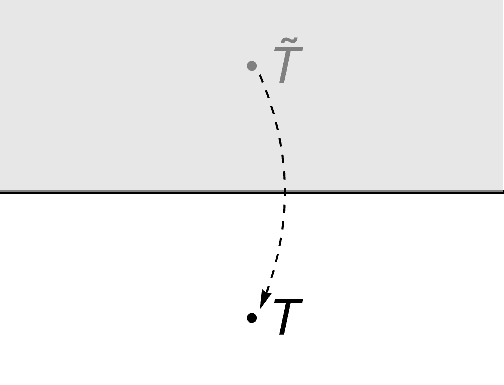
\includegraphics[width=.3\textwidth]{figures/doublingtrick.pdf}
\caption{Starting from the upper half plane with a conformal boundary condition, the doubling extends the holomorphic stress-energy tensor to the lower half plane via the identification $T(z'=\bar z) = \wt T(\bar z)$, ${\rm Im}(z)>0$.}\label{fig:doublingtrick}
\end{figure}

Splitting $X^\mu(z,\bar z) = X^\mu_L(z)+X^\mu_R(\bar z)$, we can extend the holomorphic fields $X_L^\mu, b, c$, as well as the stress-energy tensor $T$, from the upper half $z$-plane to the entire complex plane via the identification
\ie\label{doublingtrick}
& X^\mu_L(z'=\bar z) \equiv X^\mu_R(\bar z), ~~~~ \mu = 0,\cdots, p,
\\
&  X_L^i(z'=\bar z) \equiv x_0^i - X^i_R(\bar z), ~~~~ i = p+1,\cdots, 25,
\\
& b(z'=\bar z) \equiv \widetilde b(\bar z), ~~~~ c(z'=\bar z) \equiv \widetilde c(\bar z),~~~~ T(z'=\bar z) \equiv \widetilde T(\bar z),
\fe
for all $z$ with ${\rm Im}(z)\geq 0$. The boundary conditions (\ref{imzxxdp}) and (\ref{bcbdryc}) are such that the fields $X_L^\mu(z), b(z), c(z), T(z)$ remain analytic across the real axis. For instance, the boundary normal ordered operator $\vdots e^{ik_\parallel\cdot X}\vdots$, where $k_\parallel$ is parallel to the D$p$-brane world volume (i.e. $k_\parallel^i=0$, $i=p+1,\cdots,25$), is represented through the doubling trick as $e^{i 2k_\parallel\cdot X_L}$ up to an overall phase factor.\footnote{The bulk operator $e^{ik_\parallel\cdot X(z, \bar z)}$ on the UHP is represented via the doubling trick as $e^{ik_\parallel\cdot X_L(z)} e^{ik_\parallel\cdot X_L(\bar z)} =(z-\bar z)^{{\A'\over 2} k_\parallel^2}e^{ik_\parallel\cdot (X_L(z)+X_L(\bar z))}$, where the exponentials are defined via bulk normal ordering. It then follows from (\ref{bulkbdryeikx}) that the boundary normal ordered operator $\vdots e^{ik_\parallel\cdot X}\vdots$ is equivalent to $i^{{\A'\over 2} k_\parallel^2} e^{2ik_\parallel\cdot X_L(y)}$.}
The space of states on the strip that carries spacetime momentum $k_\parallel$ can be identified with ${\cal H}_{2k_\parallel}^L$, where ${\cal H}_k^L$ is defined as in (\ref{hklrfir}).

\begin{figure}[h!]
\centering
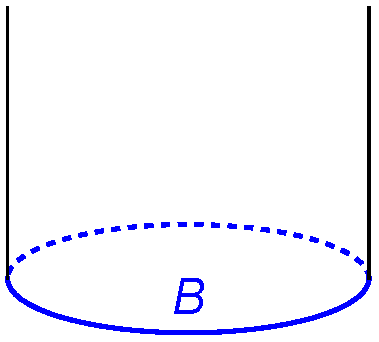
\includegraphics[width=.2\textwidth]{figures/boundarystate.pdf}
\caption{The boundary state $|B\rangle$ is created by the boundary condition $B$ on the cylinder parameterized by $w\sim w + 2\pi$ with ${\rm Im}(w)\geq 0$.}\label{fig:boundarystate}
\end{figure}

A D-brane can also be characterized in terms of a boundary state $|B\rangle$, defined as a state of the CFT on the upper half cylinder parameterized by complex coordinate $w\sim w+2\pi$ with ${\rm Im}(w)\geq 0$, created by the boundary condition at ${\rm Im}(w)=0$ (see Appendix \ref{sec:bdrystate}). It follows from (\ref{imzxxdp}) and (\ref{bcbdryc}) that
\ie\label{bcbdrytst}
(b_n - \wt b_{-n}) |B\rangle = (c_n + \wt c_{-n}) |B\rangle = (L_n - \wt L_{-n}) |B\rangle = 0, ~~~~\forall n\in\mathbb{Z}.
\fe
The boundary state $|{\rm D}p\rangle$ associated with the D$p$-brane (\ref{imzxxdp}) obeys, in addition to (\ref{bcbdrytst}),
\ie\label{dpbosbdrystcond}
& (\A_n^\mu + \wt \A_{-n}^\mu) |{\rm D}p\rangle = 0, ~~~~\forall n\in\mathbb{Z},~~~~ \mu=0,\cdots,p,
\\
& (\A_n^i - \wt \A_{-n}^i) |{\rm D}p\rangle = (\hat x^i-x^i) |{\rm D}p\rangle =0,~~~~ \forall n\in\mathbb{Z},~~~~ i=p+1,\cdots,25,
\fe 
where $\A_n^\mu,  \wt \A_n^\mu, \hat x^\mu$ are the modes of $X^\mu$ defined as in (\ref{xoope}). These conditions determine, up to the overall normalization,
\ie\label{dpbdryst}
|{\rm D}p\rangle &=  {\cal N}_{{\rm D}p} \exp\bigg[ \sum_{n=1}^\infty {1\over n} \left( -\A_{-n}^\mu \widetilde\A_{\mu,-n} +  \A_{-n}^i \widetilde\A_{-n}^i \right)  + \sum_{n=1}^\infty (c_{-n} \widetilde b_{-n} + \widetilde c_{-n} b_{-n} ) \bigg]  
\\
&~~~\times  \int {d^{25-p}k_\perp\over (2\pi)^{25-p}} e^{-ik_\perp\cdot x_0} (c_0+\wt c_0) \left|0,k_\perp; \downarrow,\downarrow \right\rangle,
\fe
where $|0,k_\perp \rangle$ corresponds to the vertex operator $e^{ik_\perp\cdot X_\perp}$, $X_\perp\equiv (X^{p+1},\cdots, X^{25})$, with vanishing $k_\parallel$. Here we adopt the normalization convention $\langle k|k'\rangle = i (2\pi)^{26}\delta^{26}(k)$, and so $\langle 0,k_\perp |0,k'_\perp \rangle = iV_{{\rm D}p}(2 \pi)^{25-p} \delta^{25-p}(k_\perp - k'_\perp)$, where $V_{{\rm D}p}$ is the spacetime volume of the D$p$-brane.

The normalization constant ${\cal N}_{{\rm D}p}$ can be determined by the following relation between the Euclidean cylinder partition function and the matrix element of the Euclidean propagator between a pair of boundary states, 
\ie\label{bccylcross}
{\rm Tr}_{{\cal H}^o} (-)^{N_{bc}} b_0 c_0 e^{-{2\pi t} L_0} = {i\over t} \langle\langle{\rm D}p| b_0 c_0 e^{-{\pi\over t} (L_0 + \wt L_0) } |{\rm D}p\rangle.
\fe
On the LHS, ${\cal H}^o$ is the space of states on the strip, or equivalently the space of boundary operators at the origin of the upper half plane (UHP), and $b_0, c_0, L_0$ are defined in terms of the holomorphic fields via the doubling trick. On the RHS, $\langle\langle{\rm D}p|$ stands for the BPZ conjugate of $|{\rm D}p\rangle$. Note that under BPZ conjugation, $\langle\langle c_{-n} \phi| =  (-)^{|\phi|+1} \langle\langle \phi| c_{n}$, $\langle\langle b_{-n} \phi| =  (-)^{|\phi|} \langle\langle \phi| b_{n}$, where $|\phi|$ is the Grassmann parity of the state $|\phi\rangle$. 

The relation (\ref{bccylcross}) can be understood in terms of the conformal map 
\ie\label{stripannuconf}
z = e^{w/t}
\fe 
that takes the periodically identified strip $0\leq {\rm Re}(w) \leq \pi$, ${\rm Im}(w) \sim {\rm Im}(w) + 2\pi t$ to the annulus $1\leq |z|\leq e^{\pi/t}$. On the RHS of (\ref{bccylcross}), we may equivalently replace the operators $b_0$ and $c_0$ acting on the boundary state with the insertion of $b_{zz}$ and $c^z$ at $z=1$. On the LHS of (\ref{bccylcross}), the operators $b_0$ and $c_0$ acting on ${\cal H}^o$ are a priori expressed in terms of the ghost fields in the $w$-frame $b_{ww}, c^w$ as
\ie\label{bzczstrip}
b_0 = -{1\over 2\pi}\int_0^{\pi} (dw\, b_{ww}(w)+d\bar w\, b_{\bar w\bar w}(\bar w)),~~~~c_0 =-{i\over 2\pi} \int_0^{\pi} (dw\, c^w(w)+d\bar w\, c^{\bar w}(\bar w)).
\fe
As only the ghost zero modes contribute, we may then replace $b_0\to - b_{ww}(0)$, $c_0\to -i c^w(0)$. Combining this with the conformal transformation (\ref{stripannuconf}) on the $b,c$ insertion then produces the factor $i/t$ on the RHS of  (\ref{bccylcross}). The normalization constant ${\cal N}_{{\rm D}p}$ in the boundary state (\ref{dpbdryst}) is then determined to be
\ie\label{ndpbosc}
{\cal N}_{{\rm D}p} = e^{-{\pi i\over 4}} 2^{-{13\over 2}} (2\pi \sqrt{\A'})^{12-p}.
\fe






\subsubsection{Open string states}

Acting on a state $|\Psi\rangle\in {\cal H}^o$ represented by the boundary operator $\Psi(0)$, the (boundary) BRST charge
\ie\label{qbodef}
Q_B^o = \int_C \left[ {dz\over 2\pi i} j_B(z) - {d\bar z\over 2\pi i} \widetilde j_B(\bar z)\right]
\fe
where $C$ is a contour in the UHP that begins on $\mathbb{R}_{+}$ and ends on $\mathbb{R}_{<0}$, is conserved and nilpotent. In the doubling trick notation, we can simply write
\ie
Q_B^o = \oint {dz\over 2\pi i} j_B(z).
\fe
A physical open string state with both ends on the D$p$-brane is represented by a $Q_B^o$-closed state $|\Psi\rangle$ subject to the Siegel constraint
\ie\label{opensiegel}
b_0 |\Psi\rangle = 0,
\fe
and two open string states differing by a $Q_B^o$-exact state are physically equivalent.

By the doubling trick, an open string state carrying spacetime momentum $k_\parallel$ parallel to the world volume of the D$p$-brane can be identified with the cohomology of $Q_B^L$ on ${\cal H}_{2k_\parallel}^L$ subject to (\ref{opensiegel}). The mass-shell condition for the open string state is
\ie\label{openmasshell}
\A' k_\parallel^2 + N - 1 = 0,
\fe
where $N\in \mathbb{Z}_{\geq 0}$ is the holomorphic oscillator level (given by the first line of (\ref{nwtnlevels})). The equivalence of the open string $Q_B^o$ cohomology to the lightcone gauge Hilbert space and OCQ Hilbert space can be proven analogously to the closed string case established in section \ref{brstlighconesec} and \ref{ocqsec}.

At level $N=0$, the only $Q_B^o$-cohomology class is represented by 
\ie
c\, \vdots e^{ik_\parallel\cdot X}\vdots ,~~~~k^2_\parallel={1\over \A'},
\fe 
which describes an open string tachyon on the D$p$-brane. The presence of the open string tachyon indicates a classical instability of the D-brane in the critical bosonic string theory.

At level $N=1$, the $Q_B^o$-cohomology classes are represented by OCQ states of the form 
\ie\label{opengaugcoll}
c\, e^\mu \vdots\partial X_\mu e^{ik_\parallel\cdot X}\vdots, ~~~~k_\parallel^2=k_\parallel\cdot e=0,
\fe
which are moreover subject to the redundancy
\ie
e^\mu \sim e^\mu + k_\parallel^\mu \zeta.
\fe
As $k_\parallel$ is parallel to the D$p$-brane, it is natural to split the states (\ref{opengaugcoll}) into two cases: $e^\mu$ parallel to the D$p$-brane, corresponding to the polarization vector of a massless vector propagating in the $(p+1)$-dimensional world volume of the D$p$-brane, and $e^\mu$ perpendicular to the D$p$-brane, giving $25-p$ massless scalar particles propagating in the world volume. The latter can be viewed as Nambu-Goldstone bosons associated with the translation symmetries in the $X^i$ directions $(i=p+1,\cdots,25)$ that are spontaneously broken by the D$p$-brane configuration. 



\subsubsection{Deformations of a D$p$-brane}


Analogously to how a marginal deformation of the worldsheet matter CFT gives rise to a deformation of the spacetime background, as seen in section \ref{sec:deformbosmat}, a marginal deformation of the boundary condition of the matter CFT gives rise to a deformation of the D-brane configuration (in a given spacetime background), which may also be equivalently viewed as turning on a background {\it open} string field.

For instance, the massless open string modes (\ref{opengaugcoll}) give rise to a gauge field $A_\mu(X)$ ($\mu=0,\cdots,p$) and scalar fields $\Phi_i(X)$, $i=p+1,\cdots, 25$ on the D$p$-brane. Turning on the background field profile $A_\mu(X)$ and $\Phi_i(X)$ amounts to deforming the worldsheet action by
\ie\label{delsbdry}
\Delta S = \int_{\partial\Sigma} ds \left[ i A_\mu(X) t^a \partial_a X^\mu - {1\over 2\pi\A'} \Phi_i(X) n^a \partial_a X^i \right],
\fe
where $t^a$ is the unit vector tangent to the boundary, and $n^a$ is the unit vector normal to the boundary pointing inward, and the operators in the integrand are defined with boundary normal ordering. In terms of the complex coordinate $z$ and the boundary vertex operators defined via the doubling trick, we can write (\ref{delsbdry}) equivalently as
\ie\label{delsbdryz}
\Delta S = \oint_{\partial\Sigma} dz \left[ 2i A_\mu(X) \partial X^\mu - {i\over \pi\A'} \Phi_i(X) \partial X^i \right] .
\fe
The marginality of the boundary deformation (\ref{delsbdry}) or (\ref{delsbdryz}) requires the integrand to be a weight 1 boundary Virasoro primary, which amounts to the condition
\ie
\Box A_\mu = \partial_\mu A^\mu = 0,~~~~\Box \Phi_i=0.
\fe
The coupling to $A_\mu$ amounts to inserting into the worldsheet path integral
\ie\label{amuxcoup}
\exp\left[ - i \int_{\partial\Sigma} A_\mu(X) dX^\mu \right].
\fe
This is identical to the action that couples an electrically charged particle to an Abelian gauge field. In particular, it means that the left and right ends of an open string carry charge $-1$ and $+1$ with respect to the gauge field $A_\mu$. 

The coupling to $\Phi_i$ amounts to the insertion of 
\ie\label{exppsigdxx}
\exp\left[ {i\over \pi\A'} \oint_{\partial\Sigma} dz\, \Phi_i(X) \partial X^i \right].
\fe
In the special case where $\Phi_i(X) = \Delta x^i$ is a constant, the effect of inserting (\ref{exppsigdxx}) is to replace the boundary state $|{\rm D}p,x_0\rangle$ of a D$p$-brane at $X^i=x_0^i$ with
\ie
\exp\left[ {i\over \pi\A'}\Delta x^i \int_0^{2\pi} dw\, \partial_w X^i \right] |{\rm D} p, x_0\rangle = e^{ - i \Delta x^i \hat k^i } |{\rm D} p, x_0\rangle = |{\rm D} p, x_0+\Delta x \rangle,
\fe
where $w$ stands for the cylinder coordinate. That is, the transverse coordinate $X^i$ of the D$p$-brane is shifted by $\Delta x^i$. This confirms the interpretation of $\Phi_i$ as the Nambu-Goldstone bosons, or the transverse collective coordinates of the D$p$-brane. Moreover, we learn that the D$p$-brane is a dynamical object: its motion in the spacetime can be equivalently described in terms of open string excitations on the D$p$-brane.


\subsubsection{Multiple D$p$-branes}

Given a pair of D-branes described by the boundary conditions $B$ and $B'$ on the worldsheet, we can consider an open string stretched between the two D-branes, with the left endpoint of the open string subject to the boundary condition $B$, and the right endpoint subject to the boundary condition $B'$. The space of states of the worldsheet CFT on the strip with left boundary condition $B$ and right boundary condition $B'$ will be denoted ${\cal H}_{BB'}$. The physical open string states are identified with the cohomology of $Q_B^o$ on ${\cal H}_{BB'}$, subject to Siegel constraint. Similarly, the open strings with the opposite orientation, stretched from $B'$ to $B$, are characterized by the BRST cohomology in ${\cal H}_{B'B}$.

%When $B$ and $B'$ correspond to parallel D$p$-branes, ${\cal H}_{BB'}$ can be constructed by a simple extension of the doubling trick (\ref{doublingtrick}), as follows. 

Under the conformal map (\ref{confzwhalf}), a state $|\psi\rangle\in {\cal H}_{BB'}$ corresponds to a boundary operator $\psi(0)$ inserted at the interface between $B$ along $\mathbb{R}_-$ and $B'$ along $\mathbb{R}_+$. Suppose $B$ represents a D$p$-brane extended along $X^0, \cdots, X^p$, with $X^i=x_0^i$, $i=p+1,\cdots, 25$, and $B'$ be the parallel D$p$-brane at $X^i = x_0^i + \Delta x^i$. Applying the doubling trick (\ref{doublingtrick}), $X_L^\mu(z)$ ($\mu=0,\cdots,p$) is analytic across both $\mathbb{R}_-$ and $\mathbb{R}_+$, whereas $X^i_L(z)$ is analytic across $\mathbb{R}_-$ and jumps by $\Delta x^i$ across $\mathbb{R}_+$, namely
\ie\label{xlldoulb}
& X_L^i(y+i\epsilon) = X_L^i(y-i\epsilon) , ~~~~ y<0,
\\
& X_L^i(y+i\epsilon) = X_L^i(y-i\epsilon) + \Delta x^i , ~~~~ y>0.
\fe
Such a discontinuity can be implemented by inserting at the origin the operator 
\ie\label{dbbpgrd}
\exp\Big(2i(k_\parallel)_\mu X_L^\mu + i {\Delta x^i \over \pi \A'} X^i_L \Big),
\fe
near which $X^i_L(z)\sim -i {\Delta x^i\over 2\pi} \log(z)$. The matter sector Hilbert space of ${\cal H}_{BB'}$ is thus constructed by acting the oscillators $\A_{-n}^\mu$, $\A_{-n}^i$ ($n\geq 1$) on (\ref{dbbpgrd}). The mass-shell condition of the stretched open string states is
\ie
k_\parallel^2 + \Big({\Delta x\over 2\pi \A' } \Big)^2 + {N - 1\over \A'} = 0,
\fe
where $N$ is the oscillator level. In particular, the level $N=1$ states contain massive vector bosons, or ``$W$-bosons'', of mass $m={|\Delta x|\over 2\pi \A'}$ and charge $(-1,+1)$ with respect to the $U(1)\times U(1)$ gauge fields on the two D$p$-branes. In the coincidence limit $\Delta x\to 0$, the $W$-bosons become massless and enhance the gauge group to $U(2)$. This is an essential feature of D-brane dynamics that will be further explored in section \ref{sec:nonabeldbrane}.

More generally, a stack of $n$ coinciding D$p$-branes is described by the direct sum boundary condition $B^{\oplus n}$, whose corresponding state space is
\ie\label{chanpatondefoneop}
{\cal H}_{B^{\oplus n}B^{\oplus n}} \simeq {\cal H}_{BB}\otimes Mat(n),
\fe
where $Mat(n)$ is the vector space of $n\times n$ complex matrices, known as the {\it Chan-Paton factor} of the boundary operator, with the boundary OPE given by (\ref{chanpatondeftwo}). 
A basis of open string states is of the form $\psi\otimes E_{ij}$, where $\psi\in {\cal H}_{BB}$ and $E_{ij}$ is the $n\times n$ matrix whose entries are $(E_{ij})_{ab}=\delta_{ia}\delta_{jb}$, representing an open string whose left and right endpoints are attached to the $i$-th and the $j$-th D$p$-brane respectively. We will see in section \ref{sec:nonabeldbrane} that the massless open string states include the vector bosons of a $U(n)$ gauge theory on the $(p+1)$-dimensional world volume, whereas all other open string states transform in the adjoint representation of the gauge group.








\subsection{BPS D-branes in type II superstring theory}
\label{sec:bpsdbrane}

A D-brane in type II superstring theory is defined by a boundary condition of the worldsheet theory that preserves the gauge invariance with respect to super-Weyl transformations and super-diffeomorphism. In the superconformal gauge, this amounts to boundary conditions of the worldsheet SCFT on the upper half $z$-plane that satisfy
\ie\label{gbetagambdry}
\lim_{{\rm Im} (z)\to 0} \left[ G(z) - \hat\eta \widetilde G(\bar z)\right]=0,
~~~~ \lim_{{\rm Im}(z)\to 0} \left[\B(z) - \hat\eta \widetilde \B(\bar z) \right] =0,~~~~  \lim_{{\rm Im}(z)\to 0} \left[\C(z) - \hat\eta \widetilde \C(\bar z) \right] = 0,
\fe
in addition to (\ref{ttboundary}), (\ref{bcbdryc}), where the sign $\hat\eta=\pm$ amounts to the choice of a spin structure associated with the boundary (see section \ref{sec:openclosedpertsuper}).

Generalizing the construction in the critical bosonic string theory, a D$p$-brane of type II superstring theory extended in the $X^0,\cdots, X^p$ directions in the 10-dimensional Minkowskian spacetime can be defined by assigning Neumann boundary condition to $X^\mu, \psi^\mu, \wt\psi^\mu$, $\mu=0,\cdots,p$, and Dirichlet boundary condition to $X^i, \psi^i, \wt\psi^i$, $i=p+1,\cdots,9$, namely (\ref{imzxxdp}) together with
\ie\label{imzpsidp}
& \lim_{{\rm Im}(z)\to 0} \big[ \psi^\mu(z) - \hat\eta\wt\psi^\mu (\bar z)\big]= 0,~~~~ \mu = 0,\cdots, p,
\\
& \lim_{{\rm Im}(z)\to 0} \big[ \psi^i(z) + \hat\eta\wt\psi^i (\bar z)\big]= 0,~~~~ i = p+1,\cdots,9,
\fe
as required by the superconformal symmetry.

The conditions (\ref{gbetagambdry}) and (\ref{imzpsidp}), however, do not entirely determine the boundary condition on the Ramond sector spin fields. One possible choice of the latter that is compatible with the OPE of the $(\psi^\mu, \B,\C)$ system is such that
\ie\label{jalbdrycond}
\lim_{{\rm Im} (z) \to 0} \left[ j_\A(z) - (\B^{p+1}\cdots \B^9 \wt j)_\A(\bar z) \right] = 0,
\fe
where $j_\A$ and $\wt j_{\widehat\A}$ are the spacetime supersymmetry currents defined as in (\ref{stsusycurrents}), and $\B^i \equiv \Gamma^i \Gamma_{11}$ is the matrix that represents parity transformation on the $so(1,9)$ spinor in the $i$-th direction. The GSO projection further requires $p$ to be an even integer in the IIA case, and an odd integer in the IIB case.

It follows from (\ref{jalbdrycond}) that the combination of spacetime supercharges
\ie\label{susydbrane}
Q_\A + (\B^{p+1}\cdots \B^9 \widetilde Q)_\A = \oint_{C} \left[ {dz\over 2\pi i} j_\A(z) - {d\bar z\over 2\pi i} (\B^{p+1}\cdots \B^9 \wt j)_\A(\bar z) \right]
\fe
is preserved by the boundary condition. Namely, (\ref{susydbrane}) vanishes when the contour $C$ is taken to be the boundary of the worldsheet $\partial\Sigma$, which allows for deriving the corresponding supersymmetry Ward identities on the superstring scattering amplitudes in the presence of the D$p$-brane (see section \ref{sec:openclosedpert}). In this sense, a flat D$p$-brane is a ${1\over 2}$-BPS object, as it preserves the 16 supersymmetries generated by $Q_\A + (\B^{p+1}\cdots \B^9 \widetilde Q)_\A$ out of the 32 supercharges of the Minkowskian background.

The space of boundary operators ${\cal H}^o$ can be conveniently constructed using the doubling trick, extending (\ref{doublingtrick}) with\footnote{Note that the sign $\hat\eta$ differs on the two sides of a Ramond operator on the boundary.}
\ie\label{doublingtrickii}
& \psi^\mu(z'=\bar z) \equiv \hat\eta\wt\psi^\mu(\bar z), ~~~~ \mu = 0,\cdots, p,
\\
&  \psi^i(z'=\bar z) \equiv - \hat\eta\wt\psi^i(\bar z), ~~~~ i = p+1,\cdots, 9,
\\
& j_\A(z'=\bar z) \equiv (\B^{p+1}\cdots \B^9 \wt j)_\A(\bar z),
\\
& \B(z'=\bar z) \equiv \hat\eta\wt \B(\bar z), ~~~~ \C(z'=\bar z) \equiv \hat\eta\wt \C(\bar z),
\fe
for all $z$ with ${\rm Im}(z)\geq 0$. In particular, the subspace of ${\cal H}^o$ carrying spacetime momentum $k_\parallel$ can be identified with ${\cal H}_{2k_\parallel}^L$ defined in (\ref{hklgsoproj}), including NS sector states of picture number $-1$ and Ramond sector states of picture number $-{1\over 2}$ subject to the holomorphic GSO projection.

\subsubsection{Open superstring states}
\label{sec:openquantii}

An open superstring state $|\psi\rangle\in {\cal H}^o$ is physical provided that it is annihilated by $Q_B^o$ (\ref{qbodef}) and obeys the Siegel constraint $b_0|\psi\rangle=0$, and also $\B_0|\psi\rangle=0$ if $|\psi\rangle$ is in the Ramond sector. Moreover, two open superstring states that differ by a $Q_B^o$-exact state are viewed as physically equivalent. The mass-shell condition for the open string states is of the form
\ie
\A'k^2 + N = 0,
\fe
where $N$ is the total oscillator weight, constrained to be a non-negative integer due to the GSO projection.

Let us inspect the massless open string states that arise at oscillator weight $N=0$. In the NS sector, the massless states are represented by the boundary vertex operator (in the doubling trick notation)
\ie\label{dsugauge}
c\, e_\mu e^{-{\phi}} \psi^\mu \vdots e^{ik_\parallel\cdot X}\vdots,~~~ k_\parallel^2=k_\parallel\cdot e =0,
\fe
where the momentum $k_\parallel$ is parallel to the D$p$-brane world volume, and $e_\mu$ is a $(p+1)$-dimensional polarization vector, subject to the redundancy $e^\mu \sim e^\mu + k_\parallel^\mu \zeta$, as well as
\ie\label{dsucoll}
c\, e^{-{\phi}} \psi^i \vdots e^{ik_\parallel\cdot X}\vdots,~~~i=p+1,\cdots,9.
\fe
Similar to the bosonic string case, (\ref{dsugauge}) describes the vector bosons of a $U(1)$ gauge field on the D$p$-brane, whereas (\ref{dsucoll}) describes $9-p$ massless scalars that are the Nambu-Goldstone bosons associated with the broken translation symmetries, or equivalently the transverse collective coordinates of the D$p$-brane.

In the R sector, the massless open string states are represented by
\ie\label{dsugoldst}
c\, u^\A  j_\A \vdots e^{ik_\parallel\cdot X}\vdots,~~~~(k_\parallel)_\mu \Gamma_{\A\B}^\mu u^\B = 0,
\fe
where $u^\A$ is a polarization spinor. (\ref{dsugoldst}) describes the massless Goldstinos associated with the 16 spacetime supersymmetries that are spontaneously broken by the D$p$-brane. Together (\ref{dsugauge}), (\ref{dsucoll}), and (\ref{dsugoldst}) form a massless multiplet of the super-Poincar\'e algebra with 16 supercharges in $(p+1)$-dimensions.


\subsubsection{The boundary state}


The boundary state $|{\rm D}p, \hat\eta \rangle$ of a BPS D$p$-brane, which comes with the spin structure assignment $\hat\eta=\pm$, takes the form
\ie\label{dpbryst}
|{\rm D}p, \hat\eta\rangle = |{\rm D}p, \hat\eta\rangle_{\rm NSNS} + |{\rm D}p, \hat\eta \rangle_{\rm RR} ,
\fe
where the (NS,NS) and (R,R) components %, expressed as
%\ie\label{nsrbdrygsop}
%& |{\rm D}p\rangle_{\rm NSNS} = {1\over 2} \big( |{\rm D}p, +\rangle_{\rm NSNS} + |{\rm D}p, - \rangle_{\rm NSNS} \big),
%\\
%& |{\rm D}p\rangle_{\rm RR} = {1\over 2} \big( |{\rm D}p, +\rangle_{\rm RR} + |{\rm D}p, - \rangle_{\rm RR} \big),
%\fe
satisfy, in addition to (\ref{bcbdrytst}), (\ref{dpbosbdrystcond}), the following conditions that follow from applying (\ref{gbetagambdry}), (\ref{imzpsidp}) to the boundary of the upper half cylinder,
\ie\label{psibdrystcond}
& (\B_r + i \hat\eta \wt \B_{-r}) |{\rm D}p, \hat\eta \rangle_{\nu} = (\C_r +  i \hat\eta \wt \C_{-r}) |{\rm D}p, \hat\eta \rangle_{\nu}  = (G_r + i\hat\eta \wt G_{-r}) |{\rm D}p, \hat\eta \rangle_{\nu}  = 0, 
\\
& (\psi_r^\mu - i\hat\eta  \wt \psi_{-r}^\mu) |{\rm D}p, \hat\eta \rangle_{\nu}  =  (\psi_r^i + i\hat\eta  \wt \psi_{-r}^i) |{\rm D}p, \hat\eta \rangle_{\nu}  =0 ,~~~~\mu=0,\cdots,p,~~~i=p+1,\cdots,9,
\fe
where $r\in \mathbb{Z}+{1\over 2}$ for $\nu={\rm NSNS}$ and $r\in \mathbb{Z}$ for $\nu={\rm RR}$, and the factor of $i$ multiplying $\hat\eta$ arises from the state/operator map on the spinor fields e.g. (\ref{psicylex}). 

The (NS,NS) component of the boundary state is determined from (\ref{psibdrystcond}) as
\ie\label{nsdryst}
|{\rm D}p,\hat\eta \rangle_{\rm NSNS} &=  \hat\eta {\cal N}_{{\rm D}p,{\rm NSNS}}  \exp\bigg[ \sum_{n=1}^\infty {1\over n} \left( -\A_{-n}^\mu \widetilde\A_{\mu,-n} +  \A_{-n}^i \widetilde\A_{-n}^i \right)
+ \sum_{n=1}^\infty (c_{-n} \widetilde b_{-n} + \widetilde c_{-n} b_{-n})
\\
&~~~~~~~~ + i \hat\eta \sum_{r\in \mathbb{Z}_{\geq 0} + {1\over 2}} \left( \psi_{-r}^\mu \widetilde\psi_{\mu,-r} - \psi_{-r}^i \widetilde\psi_{-r}^i \right) + i \hat\eta \sum_{r\in \mathbb{Z}_{\geq 0} + {1\over 2}} (\C_{-r} \widetilde \B_{-r} - \widetilde \C_{-r} \B_{-r} ) \bigg]  
\\
&~~~~~\times \int {d^{9-p}k_\perp\over (2\pi)^{9-p}} e^{ik_\perp\cdot x_0} (c_0 + \widetilde c_0) \left|0,k_\perp; \downarrow,\downarrow\right\rangle \otimes \left|-1,-1 \right\rangle,
\fe
where ${\cal N}_{{\rm D}p,{\rm NSNS}}$ is a normalization constant. The (R,R) component of the boundary state is similarly determined as
\ie\label{rrdryst}
|{\rm D}p,\hat\eta \rangle_{\rm RR} &= {\cal N}_{{\rm D}p,{\rm RR}} \exp\bigg[ \sum_{n=1}^\infty {1\over n} \left( -\A_{-n}^\mu \widetilde\A_{\mu,-n} +  \A_{-n}^i \widetilde\A_{-n}^i \right)
+ \sum_{n=1}^\infty (c_{-n} \widetilde b_{-n} + \widetilde c_{-n} b_{-n})
\\
&~~~~~~~~ + i\hat\eta \sum_{r=1}^\infty \left( \psi_{-r}^\mu \widetilde\psi_{\mu,-r} - \psi_{-r}^i \widetilde\psi_{-r}^i \right) + i \hat\eta \sum_{r=1}^\infty (\C_{-r} \widetilde \B_{-r} - \widetilde \C_{-r} \B_{-r} ) \bigg]  
\\
&~~~~~\times \int {d^{9-p}k_\perp\over (2\pi)^{9-p}} e^{ik_\perp\cdot x_0}   (c_0 + \widetilde c_0) \left|0,k_\perp; \downarrow,\downarrow \right\rangle \otimes |\Omega,\hat\eta\rangle,
\fe
where $|\Omega\rangle$ is an oscillator ground state of the $(\psi,\B,\C;\wt\psi,\wt\B,\wt\C)$ system that obeys
\ie\label{psibccond}
& (\psi_0^\mu - i \hat\eta \wt \psi_0^\mu) |\Omega,\hat\eta\rangle =  (\psi_0^i + i \hat\eta \wt \psi_0^i) |\Omega,\hat\eta\rangle =0 ,~~~~\mu=0,\cdots,p,~~~i=p+1,\cdots,9,
\\
& (\B_0 + i \hat\eta \wt \B_0) |\Omega,\hat\eta\rangle = (\C_0 +  i\hat\eta\wt \C_0) |\Omega,\hat\eta\rangle = 0.
\fe
As the boundary state should carry total holomorphic and anti-holomorphic picture number $-2$, there are two possible  picture number assignments of the RR boundary state, $(-{3\over 2}, -{1\over 2})$ or $(-{1\over 2}, -{3\over 2})$, for which (\ref{psibccond}) can be solved with
\ie\label{omagepa}
& |\Omega,\hat\eta\rangle = e^{-i\hat\eta\wt\C_0 \B_0} (e^{-{3\over 2}\phi} \Theta^T C e^{{\pi i\over 4}\hat\eta (1-\Gamma_{11})} \B^{p+1}\cdots \B^9 e^{-{1\over 2}\wt\phi} \wt\Theta), ~~~~{\rm or}
\\
& |\Omega',\hat\eta\rangle = e^{i\hat\eta \C_0 \wt\B_0} (e^{-{1\over 2}\phi} \Theta^T C e^{{\pi i\over 4}\hat\eta (1-\Gamma_{11})} \B^{p+1}\cdots \B^9 e^{-{3\over 2}\wt\phi} \wt\Theta),
\fe
where $\Theta$ and $\wt\Theta$ are the matter $so(1,9)$ spin fields with both chiralities included.

The holomorphic and anti-holomorphic fermion parity act on the boundary state (\ref{dpbryst}) by
\ie{}
&(-)^F |{\rm D}p, \hat\eta\rangle_{\rm NSNS}  =(-)^{\wt F} |{\rm D}p, \hat\eta\rangle_{\rm NSNS}  =  |{\rm D}p, -\hat\eta\rangle_{\rm NSNS},
\\
& (-)^{ F} |{\rm D}p, \hat\eta\rangle_{\rm RR} =  (-)^{p+1} (-)^{\wt F} |{\rm D}p, \hat\eta\rangle_{\rm RR} =|{\rm D}p, -\hat\eta\rangle_{\rm RR}.
\fe
It follows that the boundary state averaged over spin structures,
\ie\label{dpavg}
|{\rm D}p\rangle = {1\over 2}\big( |{\rm D}p, + \rangle + |{\rm D}p, - \rangle \big)
\fe
satisfies the type IIA (IIB) GSO projection for $p$ even (odd). The cylinder partition functions with ghost insertions and various spin structure assignments are related to the boundary states by
\ie\label{dpabr}
& {\rm Tr}_{{\cal H}^o_{-}} (-)^{N_{bc}+N_{\B\C}} b_0 c_0 e^{- 2\pi t L_0} = {-i\over t} \langle\langle {\rm D}p,+ |{}_{\rm NSNS} e^{-{\pi \over t}(L_0 + \widetilde L_0)} b_0 c_0 |{\rm D}p,+ \rangle_{\rm NSNS} ,
\\
& -{\rm Tr}_{{\cal H}^o_{+}} (-)^{N_{bc}+N_{\B\C}} b_0 c_0 %\delta(\B_0)\delta(\C_0)
e^{- 2\pi t L_0} = {-i\over t} \langle\langle {\rm D}p,- |{}_{\rm NSNS} e^{-{\pi \over t}(L_0 + \widetilde L_0)} b_0 c_0 |{\rm D}p,+ \rangle_{\rm NSNS} ,
\\
& {\rm Tr}_{{\cal H}^o_{-}} (-)^{F+N_{bc}+N_{\B\C}} b_0 c_0 e^{- 2\pi t L_0} = {-i\over t} \langle\langle {\rm D}p,+ |'_{\rm RR} e^{-{\pi \over t}(L_0 + \widetilde L_0)} b_0 c_0 %\delta(\C_0)\delta(\B_0) 
|{\rm D}p,+ \rangle_{\rm RR} ,
\\
& -{\rm Tr}_{{\cal H}^o_{+}} (-)^{F+N_{bc}+N_{\B\C}} b_0 c_0\delta(\B_0)\delta(\C_0) e^{- 2\pi t L_0} = {-i\over t} \langle\langle {\rm D}p,- |'_{\rm RR} e^{-{\pi \over t}(L_0 + \widetilde L_0)} b_0 c_0 \delta(\C_0)\delta(\B_0) |{\rm D}p,+ \rangle_{\rm RR} ,
\fe
where ${\cal H}^o_-$ and ${\cal H}^o_+$ are the space of states on the strip in the NS and R sector {\it before} GSO projection, and $|{\rm D}p,\hat\eta \rangle_{\rm RR}'$ is the $(-{1\over 2},-{3\over 2})$ picture boundary state defined by the RHS of (\ref{rrdryst}) with $\Omega$ replaced by $\Omega'$ of (\ref{omagepa}). The factor ${-i\over t}$ on the RHS arises due to the conformal transformation between the strip and the annulus, similarly to the bosonic case (\ref{bccylcross}) except for an extra minus sign due to the convention in converting the cylinder partition function to the trace.

The trace on the LHS of (\ref{dpabr}) without $(-)^F$ insertion corresponds to anti-periodic boundary condition for the worldsheet spinor fields around the Euclidean time circle, and hence the propagation of the (NS,NS) component of the boundary state along the cylinder, whereas the trace with $(-)^F$ insertion corresponds to the propagation of the (R,R) component of the boundary state. The overall minus sign multiplying ${\rm Tr}_{{\cal H}_+^o}$ is tied to the fermionic spacetime statistics of the Ramond sector open string states. Note that the trace over ${\cal H}_+^o$ on the LHS of the second equation involves a sum over degenerate ground states of the $\B\C$ system with alternating signs, and should be regularized as in (\ref{twistchareg}), (\ref{parttwsithir}). The RHS of the third equation is regularized similarly.
In the last equation, $\delta(\B_0)$ is defined as in (\ref{delbetzrer}), and similarly $\delta(\C_0)$ has the property 
\ie
\delta(\C_0)|-\tfrac{1}{2}\rangle = |-\tfrac{3}{2}\rangle, ~~~~\delta(\C_0)\C_0^n |-\tfrac{1}{2}\rangle=0,~~~ n\geq 1.
\fe
In particular, on the RHS of the last equation of (\ref{dpabr}), $\delta(\C_0)\delta(\B_0)$ eliminates the infinite degeneracy of ghost RR ground states in the $(-{3\over 2},-{1\over 2})$ picture, whereas on the LHS $\delta(\B_0)\delta(\C_0)$ eliminates the infinite degeneracy of the ghost R ground states in the $-{1\over 2}$ picture on the strip. 

The normalization constants in (\ref{nsdryst}) and (\ref{rrdryst}) are determined from (\ref{dpabr}) to be
\ie\label{ndnsnsrrres}
{\cal N}_{{\rm D}p,{\rm NSNS}} = {\cal N}_{{\rm D}p,{\rm RR}} = e^{{\pi i\over 4}} 2^{-{5\over 2}} (2\pi \sqrt{\A'})^{4-p}.
\fe
The (R,R) component of the boundary state, in particular, indicates that the D$p$-brane is a source for the RR fields. We will see in section \ref{sec:cyltypeii} and \ref{sec:dbraneeffii} that the D$p$-brane is in fact electrically charged with respect to the RR $(p+1)$-form potential (or $(p+2)$-form field strength).

An alternative D-brane boundary condition, known as the {\it anti-D$p$-brane} or $\overline{{\rm D}p}$-brane, can be constructed by flipping the sign of anti-holomorphic spin fields in (\ref{jalbdrycond}), (\ref{doublingtrickii}), which leaves the open string spectrum invariant but flips the sign of the (R,R) component of the boundary state (\ref{dpbryst}). For $1\leq p\leq 8$, the $\overline{{\rm D}p}$-brane can be obtained from the D$p$-brane by applying a spacetime rotation by $\pi$ in the $(X^p,X^{p+1})$-plane. In other words, the $\overline{{\rm D}p}$-brane can simply be viewed as the D$p$-brane with the opposite orientation, thereby carrying the opposite charge with respect to the RR fields.





\subsection{Non-BPS D-branes}
\label{sec:nonbpsdbranes}

Consider a pair of coincident D$p$ and $\overline{{\rm D}p}$-branes in either type IIA ($p$ even) or IIB ($p$ odd) string theory, whose corresponding boundary conditions are denoted $B$ and $\overline B$ respectively. The boundary condition $B\oplus \overline{B}$ of the D$p$-$\overline{{\rm D}p}$ system is characterized by (\ref{ttboundary}), (\ref{bcbdryc}), (\ref{imzxxdp}), (\ref{gbetagambdry}), (\ref{imzpsidp}) as for a D$p$-brane, but with the boundary condition on spin fields (\ref{jalbdrycond}) replaced by
\ie\label{jalbdryconddpbar}
& \lim_{z\to y} j_\A(z) = j_\A(y)\otimes \mathbb{I},
\\
& \lim_{z\to y} (\B^{p+1}\cdots \B^9 \wt j)_\A(\bar z) = j_\A(y)\otimes \sigma_3,~~~~y\in \mathbb{R},
\fe
where the Chan-Paton factors $\mathbb{I}$ and $\sigma_i$ stand for the $2\times 2$ identity matrix and Pauli matrices respectively. On the RHS of (\ref{jalbdryconddpbar}), $j_\A(y)\otimes {\mathbb{I}+\sigma_3\over 2}$ is viewed as a boundary operator in ${\cal H}_{BB}$, whereas $j_\A(y)\otimes {\mathbb{I}-\sigma_3\over 2}$ is viewed as a boundary operator in ${\cal H}_{\overline B\overline B}$. More generally, we can express a boundary operator in ${\cal H}_{B\oplus \overline B,B\oplus \overline B}$ as
\ie
\begin{pmatrix} \psi_{BB} & \psi_{B\overline B} \\ \psi_{\overline BB} & \psi_{\overline B\overline B} \end{pmatrix},
\fe
where $\psi_{BB}\in {\cal H}_{BB}$, etc.


The space ${\cal H}_{B\overline B}$, which describes open strings stretched between the D$p$ and $\overline{{\rm D}p}$-branes, can be constructed as ${\cal H}_{BB}$ but with the opposite open string GSO projection. That is, the subspace of ${\cal H}_{B\overline B}$ carrying spacetime momentum $k_\parallel$ is isomorphic to the subspace of ${\cal H}^L_{2k_\parallel}$ that obeys $(-)^F=-1$. In the NS sector, the projection $(-)^F=-1$ retains the open string tachyon represented by the boundary operator 
\ie
c e^{-\phi} \vdots e^{ik_\parallel\cdot X}\vdots \otimes \begin{pmatrix} 0 & 1 \\ 0 & 0 \end{pmatrix},~~~~k_\parallel^2 = {1\over 2\A'},
\fe
while removing the massless bosonic states of the form (\ref{dsugauge}). In the R sector, on the other hand, massless fermionic open string states of the opposite spacetime chirality as (\ref{dsugoldst}), namely
\ie\label{dsugoldstbar}
c\, u^\da  e^{-{\phi\over 2}} \Theta_\da \vdots e^{ik_\parallel\cdot X}\vdots \otimes \begin{pmatrix} 0 & 1 \\ 0 & 0 \end{pmatrix},~~~~k_\parallel^2 =(k_\parallel)_\mu \Gamma_{\da\db}^\mu u^\db = 0,
\fe
are retained. The space ${\cal H}_{\overline B B}$ can be constructed similarly.

Note that the boundary Ramond operator $j_\da' \equiv e^{-{\phi\over 2}} \Theta_\da$, which exists in both ${\cal H}_{B\overline B}$ and ${\cal H}_{\overline B B}$, is related to the GSO-unprojected bulk spin field by
\ie\label{jalddbar}
& \lim_{z\to y} e^{-{\phi\over 2}} \Theta_\da(z) = j'_\da(y)\otimes i\sigma_2,
\\
& \lim_{z\to y} e^{-{\wt\phi\over 2}}(\B^{p+1}\cdots \B^9 \wt \Theta)_\da(\bar z) = j'_\da(y)\otimes \sigma_1,~~~~y\in \mathbb{R}.
\fe

It is possible to construct a new boundary condition $\widetilde B$ by {\it reinterpreting} $B\oplus \overline B$ (subject to restrictions on the admissible boundary operators) as that of the bulk SCFT defined with a different chiral GSO projection, namely $(-)^F = (-)^{\wt F} \iota =1$ where $\iota$ flips the sign of the anti-holomorphic Ramond sector states, such that
\ie\label{hbbproj}
{\cal H}_{\wt B\wt B} = \mathbb{P}_{\sigma_1} {\cal H}_{B\oplus \overline B,B\oplus \overline B},
\fe
where $\mathbb{P}_{\sigma_1}$ stands for the projection onto states that are invariant under $\psi\mapsto \sigma_1\psi\sigma_1$, i.e. those carrying Chan-Paton factors $\mathbb{I}$ and $\sigma_1$. In particular, the first equation (\ref{jalbdryconddpbar}) and the second equation of (\ref{jalddbar}) are now viewed as valid relations between the GSO-projected bulk and boundary operators.

The boundary condition $\wt B$ can be interpreted as that of a {\it non-BPS D$p$-brane} in the type II string theory of the opposing type of GSO projection, i.e. type IIA for $p$ odd and type IIB for $p$ even. The open string states that arise from the NS sector of ${\cal H}_{\wt B\wt B}$ include the massless vector boson and scalars
\ie\label{dsugaugenonbps}
& c\, e_\mu e^{-{\phi}} \psi^\mu \vdots e^{ik_\parallel\cdot X} \vdots \otimes \mathbb{I}, ~~~~ k_\parallel\cdot e =0,
\\
& c\, e^{-{\phi}} \psi^i \vdots e^{ik_\parallel\cdot X}\vdots \otimes \mathbb{I},~~~i=p+1,\cdots,9,~~~k_\parallel^2=0,
\fe
and the open string tachyon
\ie\label{ddbartach}
c e^{-\phi} \vdots e^{ik_\parallel\cdot X}\vdots \otimes \sigma_1,~~~~k_\parallel^2 = {1\over 2\A'}.
\fe
The presence of a single set of collective coordinates (second line of (\ref{dsugaugenonbps})) indicates that $\wt B$ describes a single D-brane (as opposed to, say, a pair of D-branes). The presence of the open string tachyon indicates that the non-BPS D-brane is classically unstable.
The open string states from the R sector of ${\cal H}_{\wt B\wt B}$ include the massless fermions
\ie{}
& c\, u^\A  j_\A \vdots e^{ik_\parallel\cdot X}\vdots \otimes \mathbb{I},~~~~ k_\parallel^2 =(k_\parallel)_\mu \Gamma_{\A\B}^\mu u^\B = 0,
\\
& c\, \wt u^\da  j_\da' \vdots e^{ik_\parallel\cdot X}\vdots \otimes \sigma_1,~~~~k_\parallel^2 =(k_\parallel)_\mu \Gamma_{\da\db}^\mu \wt u^\db = 0,
\fe
which are the Goldstinos associated with the 32 supersymmetries spontaneously broken by the non-BPS D$p$-brane.




The boundary state of the non-BPS D$p$-brane is simply
\ie\label{nonbpsbdryst}
|\wt B,\hat\eta \rangle =  \sqrt{2}|{\rm D}p, \hat\eta \rangle_{\rm NSNS},
\fe
where $|{\rm D}p, \hat\eta \rangle_{\rm NSNS}$ is defined as in (\ref{nsdryst}), except that now $p$ is odd in type IIA theory and even in type IIB theory. In particular, the non-BPS D-branes are uncharged with respect to the RR fields.
Indeed, one can verify the cylinder modular crossing relations
\ie\label{dpabrnonbps}
& {\rm Tr}_{\wt{\cal H}^o_{\rm NS}} (-)^{N_{bc}+N_{\B\C}} b_0 c_0 e^{- 2\pi t L_0} = {i\over t} \langle\langle {\rm D}p,+ |{}_{\rm NSNS} e^{-{\pi \over t}(L_0 + \widetilde L_0)} b_0 c_0 |{\rm D}p,+ \rangle_{\rm NSNS} ,
\\
& -{\rm Tr}_{\wt{\cal H}^o_{\rm R}} (-)^{N_{bc}+N_{\B\C}} b_0 c_0\delta(\B_0)\delta(\C_0) e^{- 2\pi t L_0} = {i\over t} \langle\langle {\rm D}p,- |{}_{\rm NSNS} e^{-{\pi \over t}(L_0 + \widetilde L_0)} b_0 c_0 |{\rm D}p,+ \rangle_{\rm NSNS}  ,
\fe
where $\wt{\cal H}^o_{\rm NS}$ and $\wt{\cal H}^o_{\rm R}$ are the NS and R sector subspaces of ${\cal H}_{\wt B\wt B}$. Note that while the spectrum of $\wt{\cal H}^o_{\rm NS}$ and $\wt{\cal H}^o_{\rm R}$ is isomorphic to that of ${\cal H}^o_-$ and ${\cal H}^o_+$ appearing in (\ref{dpabr}), the former is not subject to GSO projection (as is compatible with the $\sqrt{2}$ factor in (\ref{nonbpsbdryst})).



%We can also consider the open strings stretched between the non-BPS $\widetilde{\rm D}p$-brane and a BPS D$(p+1)$-brane extended in $X^0,\cdots, X^{p+1}$ directions. The corresponding cylinder partition function is
%\ie{}
%& \langle\langle \widetilde{\rm D}p| e^{-{\pi i\over \tau}(L_0 + \widetilde L_0)}  |{\rm D}(p+1)\rangle = {1\over \sqrt{2}} \langle\langle {\rm NSNS},p| e^{-{\pi i\over \tau}(L_0 + \widetilde L_0)}  |{\rm NSNS},p+1\rangle 
%\\
%&= V_{p+1} \int {d^{p+1} k_\parallel\over (2\pi)^{p+1}} e^{2\pi i \tau \A' k^2_\parallel} {(\theta_3(0|\tau))^{7\over 2} ({1\over 2}\theta_2(0|\tau))^{1\over 2}\over (\eta(\tau))^{12}} 
%\\
%&= V_{p+1} \int {d^{p+1} k_\parallel\over (2\pi)^{p+1}} e^{2\pi i \tau \A' k^2_\parallel} {1\over (\eta(\tau))^8} q^{-{5\over 48}} \prod_{n=0}^\infty (1+q^{n+{1\over 2}})^7 \prod_{m=1}^\infty (1+q^m) ,
%\fe
%which indeed takes the form of a trace over an open string Hilbert space.







\subsection{More general configurations of D-branes}


\subsubsection{Intersecting D-branes}
\label{sec:intbrane}

The analysis of open superstring spectrum in section \ref{sec:openquantii} can be generalized to open strings stretched between a D$p$-brane and a D$p'$-brane which need not be parallel to one another, and $p'$ need not be equal to $p$.  

To begin with, consider a BPS D$p$-brane that extends in the $X^0,\cdots, X^p$ directions, whose transverse coordinates are fixed to $X^{p+1}=\cdots =X^9=0$, and a BPS D$p'$-brane that extends in $X^0, \cdots, X^q$, $X^{p+1},\cdots, X^{p+p'-q}$, whose transverse coordinates are fixed to $X^{q+1}=\cdots = X^p = X^{p+p'-q}=\cdots X^9=0$. The worldsheet of an open string stretched between the D$p$ and the D$p'$-branes is subject to Neumann (N) boundary condition in the $X^0,\cdots, X^q$ directions, Dirichlet (D) boundary condition in the $X^{p+p'-q},\cdots, X^9$ directions, and mixed (N,D) or (D,N) conditions on the (left,right) boundaries in the $X^{q+1},\cdots,X^{p+p'-q}$ directions.

The space of states ${\cal H}_{\rm ND}$ of a free boson $X$ subject to (N,D) condition on the (left,right) boundary of strip can be constructed using a generalization of the doubling trick. Mapping the strip to the UHP, and extending $X_L(z)$ to the complex plane by the identification (\ref{doublingtrick}), $X_L(z)$ is analytic across $\mathbb{R}_-$ and changes sign across $\mathbb{R}_+$, namely
\ie\label{xlldoulbndmix}
& X_L(y+i\epsilon) = X_L(y-i\epsilon) , ~~~~ y<0,
\\
& X_L(y+i\epsilon) = - X_L(y-i\epsilon)  , ~~~~ y>0.
\fe
In other words, as $z$ circles around the origin, $X_L(z)$ flips sign. ${\cal H}_{\rm ND}$ can thus be identified with the twisted sector of the $\mathbb{Z}_2$ orbifold of the chiral boson (section \ref{orbifoldsection}). In particular, the ground state of ${\cal H}_{\rm ND}$ can be identified with the holomorphic twist field $\sigma$, whose conformal weight is $h={1\over 16}$  (see (\ref{sigmatwistwei})). The Laurent series of $X_L(z)$ takes the form
\ie\label{chiralbostwisexp}
X_L(z)= i \sqrt{\A'\over 2} \sum_{r\in\mathbb{Z}+{1\over 2}} {1\over r} {\A_r \over z^r} ,
\fe
where the oscillator $\A_r$ lowers $L_0$ by a half-integer $r$, with $\A_r |\sigma\rangle = 0$ for all $r\geq {1\over 2}$. A similar analysis applies to the free boson subject to (D,N) boundary condition on the strip.

The state of the free fermion $(\psi,\wt\psi)$ theory subject to (N,D) boundary condition on the strip can be constructed similarly. After mapping to the UHP and applying the doubling trick, $\psi(z)$ has the Laurent series
\ie
\psi(z) = \sum_{r\in \mathbb{Z}+\nu + {1\over 2}} {\psi_r\over z^{r+{1\over 2}}},
\fe
where $\nu={1\over 2}$ in the NS sector and $\nu=0$ in the R sector. An NS sector ground state is thus a weight ${1\over 16}$ operator $\tau$ that obeys $\psi_r |\tau\rangle = 0$ for all $r\geq 1$, and $\psi_0|\tau\rangle = \pm {1\over \sqrt{2}} |\tau\rangle$, whereas the R sector ground state is a weight 0 ``identity interface'' operator $\iota$ that obeys $\psi_r |\iota\rangle=0$ for all $r\geq {1\over 2}$. The free fermion subject to (D,N) boundary condition can be treated similarly.

As $p'$ differs from $p$ by an even integer, the total number of (N,D) and (D,N) directions $d_{\rm ND}\equiv p+p'-2q$ is even. The NS sector oscillator ground state of the matter SCFT on the strip subject to (D$p$, D$p'$) boundary condition is of the form
\ie\label{nsndbdry}
\Sigma S_a \vdots e^{ik_\parallel\cdot X}\vdots,
\fe
where $\Sigma$ is the product of $d_{\rm ND}$ $\mathbb{Z}_2$ twist fields of the chiral bosons, of conformal weight ${d_{\rm ND}\over 16}$, and $S_a$ is the spin field of the $d_{\rm ND}$ chiral fermions that transforms in the spinor representations of $so(d_{\rm ND})$, also of weight ${d_{\rm ND}\over 16}$. The momentum $k_\parallel$ is restricted to the $(q+1)$-dimensional intersection between the D$p$ and the D$p'$-brane. Upon GSO projection, (\ref{nsndbdry}) gives rise to the lowest level NS sector D$p$-D$p'$ open string states that are bosons living at the brane intersection, whose mass squared is given by\footnote{This formula is not applicable in the $d_{\rm ND}=0$ case, of course, as the NS oscillator ground state is eliminated by the GSO projection.}
\ie\label{mkdnd}
m^2 = - k_\parallel^2 = {1\over \A'} \left( {d_{\rm ND}\over 8} - {1\over 2} \right).
\fe
The R sector oscillator ground state of the matter SCFT on the strip takes the form
\ie\label{rndbdry}
\Sigma \Theta_\A \vdots e^{ik_\parallel\cdot X}\vdots,
\fe
where $\Theta_\A$ is the spin field of $10-d_{\rm ND}$ chiral fermions corresponding to the (N,N) and (D,D) directions, that transforms in the spinor representations of $so(1,9-d_{\rm ND})$ and has conformal weight ${10-d_{\rm ND}\over 16}$. After including the ghost spin field and the GSO projection, the resulting R sector D$p$-D$p'$ open string states are {\it massless} fermions (i.e. $k_\parallel^2=0$) living at the brane intersection.

Let us note that in the above intersecting brane setting, while the D$p$-brane preserves the supercharge
\ie\label{epssuperq}
\epsilon^\A Q_\A + \wt \epsilon^{\widehat\A} \wt Q_{\widehat\A}
\fe 
for $\wt\epsilon = (\B^{p+1}\cdots \B^9)^T \epsilon$, the D$p'$-brane preserves (\ref{epssuperq}) for $\wt\epsilon = (\B^{q+1}\cdots\B^p\B^{p+p'-q}\cdots \B^9)^T \epsilon$. Common supercharges preserved by the D$p$-D$p'$ system exist only if $\prod_{a\in {\rm ND, DN}}\B^a$ has eigenvalue 1, which occurs when $d_{\rm ND} \equiv 0$ mod 4. In this case, the D$p$-D$p'$ system is ${1\over 4}$-BPS, in the sense that 8 out of the 32 supercharges of type II string theory is preserved. 

When $d_{\rm ND}\equiv 2$ mod 4, on the other hand, supersymmetry is broken entirely. In particular, in the case $d_{\rm ND}= 2$, there is an NS open string tachyon mode as seen from (\ref{mkdnd}), leading to a classical instability.

\subsubsection{D-branes at angles}
\label{sec:angles}

We now consider more general D-branes configurations, starting with the example of a pair of D1-branes intersecting at an angle. We may assume that the first D1-brane is extended along the $X^1$ direction, with $X^2=\cdots=X^9=0$, and the second D1-brane, which we refer to as D$1'$, is at angle $\theta$ in the $(X^1,X^2)$-plane, i.e. extended along $X^2 = X^1 \tan\theta$, with $X^3=\cdots= X^9=0$. 

The D1-D$1'$ open string is described by the worldsheet CFT on the strip subject to the boundary conditions $(B,B')$ on the (left,right) boundaries, where $B$ stands for Neumann in the $X^1$ direction and Dirichlet in the $X^2$ direction, and $B'$ is related to $B$ via an $SO(2)$ rotation by the angle $\theta$. Writing $Z\equiv X^1+i X^2$, after mapping the strip to the UHP and applying the doubling trick, $Z$ on the UHP is replaced by the holomorphic field $Z_L= X_L^1 + i X_L^2$ on the complex plane that obeys the matching condition
\ie\label{zlldoulbndmix}
& Z_L(y+i\epsilon) = \overline Z_L(y-i\epsilon) , ~~~~ y<0,
\\
& e^{-i\theta} Z_L(y+i\epsilon) = e^{i\theta} \overline Z_L(y-i\epsilon)  , ~~~~ y>0,
\fe
across the real axis. We can further define
\ie{}
& \wt Z_L(z) \equiv Z_L(z), ~~~~{\rm Im}(z)>0,
\\
& \wt Z_L(z) \equiv \overline Z_L(z), ~~~{\rm Im}(z)<0,
\fe
so that (\ref{zlldoulbndmix}) amounts to the monodromy condition
\ie
Z_L(e^{2\pi i } z) = e^{-2i\theta} Z_L(z)
\fe
across the positive real axis. The ground state of the $(X^1, X^2)$ system subject to $(B, B')$ boundary condition can be identified with a twist field $\sigma(0)$, around which $Z_L(z)$ admits the Laurent series expansion
\ie\label{zlmodexp}
Z_L(z) = i \sqrt{\A'\over 2} \sum_{r\in \mathbb{Z} - \theta/\pi} {1\over r} {\A_r\over z^r},
\fe
where the grading $r$ of the oscillators $\A_r$ is an integer shifted by $-{\theta/ \pi}$, with $\A_r|\sigma\rangle=0$ for all positive $r$. Assuming without loss of generality $\theta\in (0,\pi)$, by a calculation essentially identical to (\ref{fourpointratiozzbar}), one can determine the weight of $\sigma$ to be ${1\over 2} {\theta\over \pi} \Big(1-{\theta\over \pi}\Big)$.

A similar analysis applies to the fermions $\Psi \equiv {1\over \sqrt{2}}( \psi^1 + i \psi^2)$, $\overline\Psi \equiv {1\over \sqrt{2}}(\psi^1 - i \psi^2)$, which admits the Laurent series
\ie\label{psizmodexp}
\Psi(z) = \sum_{r\in \mathbb{Z} + \nu - \theta/\pi} {\Psi_r\over z^{r+{1\over 2}}},~~~~ \overline\Psi(z) = \sum_{r\in \mathbb{Z} + \nu + \theta/\pi} {\overline\Psi_r\over z^{r+{1\over 2}}},
\fe
where $\nu={1\over 2}$ in the NS sector and $\nu=0$ in the R sector. In the bosonized representation (\ref{psiha}), we may identify $\Psi \simeq e^{i H}$ where $H$ is a chiral boson that obeys the OPE $H(z) H(0)\sim -\log(z)$. Assuming $\theta\in [0, \pi]$, the two lowest NS sector states are 
\ie\label{twolowns}
& \tau \simeq e^{i{\theta\over \pi} H},
\\
& \tau' = \overline \Psi_{-{1\over 2} + {\theta\over \pi}}\tau \simeq e^{i({\theta\over \pi}-1) H},
\fe
whose conformal weights are ${1\over 2} ({\theta\over \pi})^2$ and ${1\over 2} ({\pi-\theta\over \pi})^2$ respectively. Note that $\tau$ is the NS ground state for $\theta\in (0,{\pi\over 2})$, whereas $\tau'$ is the NS ground state for $\theta\in ({\pi\over 2}, \pi)$. At $\theta={\pi\over 2}$, there is a 2-fold degeneracy of the NS ground states -- this is precisely the $d_{\rm ND}=2$ case analyzed in section \ref{sec:intbrane}.

%Note that $\tau'$ and $\tau$ have opposite fermion parity $(-)^F$.

Combining with the rest of the matter SCFT subject to Neumann boundary condition in $X^0$ and Dirichlet boundary condition in $X^3,\cdots, X^9$ directions, one finds that the lowest open string mode in the NS sector that survives the GSO projection is represented by the vertex operator
\ie\label{dangltach}
c\, e^{-\phi} \sigma \tau' \vdots e^{-i \omega X^0}\vdots ,
\fe
whose mass-shell condition is
\ie
\omega^2 = {1\over \A'} \left[ {1\over 2} {\theta\over \pi} \Big(1-{\theta\over \pi}\Big) + {1\over 2} \Big({\pi-\theta\over \pi}\Big)^2 - {1\over 2}\right] = - {\theta \over 2\pi \A'}.
\fe
This result is in agreement with (\ref{mkdnd}) at $\theta = {\pi\over 2}$, and with (\ref{ddbartach}) at $\theta=\pi$. For nonzero $\theta$, the open string mode (\ref{dangltach}) is tachyonic, indicating that the intersecting D1-D$1'$ system is unstable. Indeed, the energy of the system can be lowered by reconnecting the D1 and D$1'$-branes.


Next, consider a pair of D2-branes at angles. We may assume that the first D2-brane is extended along $X^1$ and $X^3$ directions, with $X^2=X^4=\cdots=X^9=0$, and that the configuration of the second D$2$-brane, which we refer to as D$2'$, is related by a rotation by angle $\theta_1$ in the $(X^1,X^2)$-plane, and by angle $\theta_2$ in the $(X^3, X^4)$-plane. The D2-D$2'$ open strings can be understood by applying (\ref{zlmodexp}) and (\ref{psizmodexp}) to the worldsheet bosons and fermions corresponding to the 12 and 34 directions separately. Assuming $\theta_1, \theta_2\in (0,\pi)$, the lowest open string modes in the NS sector that survives the GSO projection are represented by the vertex operators
\ie\label{openddtwos}
& c \, e^{-\phi} \sigma_{12}\sigma_{34} \tau_{12} \tau_{34}' \vdots e^{-i\omega_1 X^0}\vdots ,~~~~ c \, e^{-\phi} \sigma_{12}\sigma_{34} \tau_{12}' \tau_{34} \vdots e^{-i\omega_2 X^0}\vdots ,
%\\
%& c \, e^{-\phi} \sigma_{12}\sigma_{34} \tau_{12} \tau_{34}\psi^i e^{-i\omega_3 X^0},~~~~ c \, e^{-\phi} \sigma_{12}\sigma_{34} \tau_{12}' \tau_{34}' \psi^i e^{-i\omega_4 X^0},~~~~ i = 0, 5,\cdots,9.
\fe
whose mass-shell conditions are
\ie
\omega_1^2 = {\theta_1 - \theta_2 \over 2\pi \A'},~~~~ \omega_2^2 = {\theta_2 - \theta_1 \over 2\pi \A'}. %,~~~~ \omega_3^2 = {\theta_1 + \theta_2 \over 2\pi \A'},~~~~ \omega_4^2 = {2\pi - \theta_1 - \theta_2 \over 2\pi \A'}.
\fe
The condition for the absence of open string tachyon is $\theta_1=\theta_2$, in which case the open string modes (\ref{openddtwos}) are massless, and in fact give rise to moduli deformations of the D2-D$2'$ system.

Moreover, the supercharges preserved by the D2-D$2'$ system are given by (\ref{epssuperq}) for $\epsilon, \wt\epsilon$ that obey
\ie\label{epsdtdt}
\wt\epsilon = (\B^2 \B^4 \cdots\B^9)^T\epsilon = R^{-1} (\B^2 \B^4 \cdots\B^9)^T R \epsilon,~~~~ R = \exp\left( {\theta_1\over 2} \Gamma_{12} + {\theta_2\over 2} \Gamma_{34} \right).
\fe
The existence of nontrivial solutions to (\ref{epsdtdt}) requires $R^2$ to have eigenvalue 1 on a spinor of definite chirality, which occurs precisely at $\theta_1=\theta_2$. In this case, the D2-D$2'$ system is ${1\over 4}$-BPS. Writing
\ie
U \equiv X^1 + i X^3,~~~~ V \equiv X^2+i X^4,
\fe
the D2-D$2'$ configuration can be expressed as the locus
\ie\label{uvgeomsimp}
(U, V) \in \mathbb{C}^2:~ V(V - U \tan \theta) = 0.
\fe
We will see in section \ref{sec:wrappeddbranes} that the effect of turning on the open string fields corresponding to the massless modes (\ref{openddtwos}) is to deform the geometry of (\ref{uvgeomsimp}) to
\ie\label{deformttuv}
(U, V) \in \mathbb{C}^2:~ V(V - U \tan \theta) = t,
\fe
where $t$ is a complex parameter.

Finally, let us mention that a double Wick rotation of the target spacetime coordinates would relate the D-brane at an angle to a D-brane moving at constant velocity. In section \ref{sec:dzerodyn} this will be applied to analyze the scattering of D0-branes.



%\subsubsection{Marginal deformations of D-branes}


%\fixme{D-brane junctions}












\newpage



\section{D-brane dynamics in bosonic string theory}
\label{sec:openamp}

\subsection{Open+closed bosonic string perturbation theory}
\label{sec:openclosedpert}

The scattering theory of closed strings in the spacetime and open strings on D-branes can be formulated through the path integral over worldsheet with boundaries. In the conformal gauge, while closed string asymptotic states are represented by BRST-closed vertex operators ${\cal V}_i^c$ inserted at punctures on a Riemann surface $\Sigma$, open string asymptotic states are represented by boundary vertex operators ${\cal V}_j^o$ inserted at boundary punctures on $\partial\Sigma$. The bosonic open+closed string amplitude with $n$ closed string states and $m$ ($\geq 1$) open string states, generalizing the closed string amplitude (\ref{omegaone}), takes the form
\ie\label{openampbos}
& {\cal A} \left[\{V_i^c\}_{1\leq i\leq n}, \{V_j^o\}_{1\leq j\leq m}\right] = \sum_{h=0}^\infty \sum_{b=1}^\infty {\cal A}_{h,b} \left[\{V_i^c\}_{1\leq i\leq n}, \{V_j^o\}_{1\leq j\leq m}\right],
\\
& {\cal A}_{h,b} \left[\{V_i^c\}_{1\leq i\leq n}, \{V_j^o\}_{1\leq j\leq m}\right] = N_{h,n;b, m} \int_{{\cal M}_{h,n;b,m}} \Omega_{6h-6+3b + 2n + m},
\fe
where ${\cal M}_{h,n; b,m}$ is the moduli space of a Riemann surface of genus $h$, $b$ boundary components, $n$ bulk punctures and $m$ boundary punctures, whose dimension is equal to $6h-6+3b + 2n + m$. $N_{h,n;b, m}$ is a normalization constant to be fixed by consideration of unitarity, and $\Omega_p$ is the degree $p$ component of the differential form
\ie\label{omegaopencl}
\Omega = \left\langle e^{\cal B} \prod_{i=1}^n {\cal V}_i^c \prod_{j=1}^m {\cal V}_j^o \right\rangle_{\Sigma},
\fe
where the correlator is that of the matter+ghost CFT subject to the D-brane boundary condition on $\partial\Sigma$.
The 1-form ${\cal B}$ is defined as in (\ref{calboneform}), where ${\cal B}_{t^k}$ is constructed as (\ref{bkfactor}) except that the contour segments $C_{j\ell}$ may end on the boundary $\partial\Sigma$. 

Let us note that the moduli space ${\cal M}_{h,n; b,m}$ comes with an orientation concerning the ordering of the moduli associated with each of the boundary components, which affects the overall sign of the integration measure. This is consistent with our convention in which the boundary state $|B\rangle$ of a D-brane is Grassmann-odd (recall e.g. (\ref{dpbdryst})). The specification of the orientation of the moduli space, or equivalently the sign convention for the integration measure on the moduli space, will be illustrated through the example of the cylinder amplitude in section \ref{sec:cylinderamp}.\footnote{A general prescription for specifying the orientation of the moduli space of Riemann surfaces with boundary is given by Sen and Zwiebach, arXiv:2405.03784.}

We define the BPZ conjugate $\langle\langle\psi|$ of a state on the strip $|\psi\rangle$ by
\ie\label{bpzconjdefbdr}
\langle \langle \psi|\phi\rangle \equiv \left\langle [\psi(0)]^{I'} \phi(0)\right\rangle_{D^2},
\fe
where $I'$ stands for the inversion map $z' = -1/z$. A basis of open string 1-particle states $|k_\parallel; \C\rangle^o$, when $k_\parallel$ is the momentum along the D$p$-brane world volume and $\C$ labels the internal quantum numbers, is normalized with
\ie
{}^o\langle k_\parallel;\C|k'_\parallel; \C\rangle^o = 2k^0_\parallel (2\pi)^p \delta^p (k_\parallel-k'_\parallel) \delta_{\C\C'}.
\fe
The corresponding boundary vertex operators of the OCQ form, ${\cal V}_\C^o(k_\parallel)= c V_\C^o(k_\parallel)$ where $V_\C^o(k_\parallel)$ is a matter boundary primary of weight 1, are normalized with
\ie\label{vvopennorm}
\langle\langle \overline{{\cal V}_\C^o(k'_\parallel)} | c_0 | {\cal V}_{\C'}^o(k_\parallel)\rangle = K_o \delta_{\C\C'} i (2\pi)^{p+1} \delta^{p+1}(k_\parallel-k'_\parallel), 
\fe
analogously to that of the closed string states (\ref{vvnormvonv}).  Here $\overline{{\cal V}_\C^o(k_\parallel)}\equiv c \overline{V_\C^o(k_\parallel)}$, where $\overline{V_\C^o(k_\parallel)}$ is the Hermitian conjugate of the matter primary $V_\C^o(k_\parallel)$. The normalization constant $K_o$ will be determined by the consistency with unitarity below.


Consider the surface $\Sigma$ constructed by gluing $\Sigma_1$ and $\Sigma_2$ via the open string analog of the plumbing fixture, where the annuli regions of a pair of half-discs 
\ie\label{pairdiscsg}
D_1^o = \{z:|z|<1, {\rm Im}(z)>0\} \subset \Sigma_1,~~~~D_2^o = \{z':|z'|<1, {\rm Im}(z')>0\} \subset \Sigma_2,
\fe
are identified via the plumbing map
\ie\label{openplumbing}
z' = - {e^{-2\pi t}\over z},
\fe
for some $t>0$. The contribution to the string amplitude from the degeneration limit $t\gg 0$ is of the form
\ie\label{nnopenaf}
N_{h,n;b, m} \int_0^\infty dt \langle\langle S_2 | {\cal B}_t e^{-2\pi t L_0} |S_1\rangle ,
\fe
where $|S_i\rangle$ are the open string surface states associated with $\Sigma_i\backslash D_i^o$ analogously to those of (\ref{ampnearxxb}). ${\cal B}_t$ is the $b$ ghost insertion associated with the modulus $t$, computed using the doubling trick as
\ie
{\cal B}_t = \oint {dz\over 2\pi i} b_{zz}\left.{\partial z\over \partial t}\right|_{z'} = - 2\pi b_0.
\fe
(\ref{nnopenaf}) thus evaluates to
\ie\label{nnopenafb}
- N_{h,n;b, m} \langle\langle S_2 | {b_0\over L_0} |S_1\rangle.
\fe
As the momentum $P_\parallel$ of $|S_1\rangle$ approaches the physical momentum of an open string state $|k_\parallel;\C\rangle^o$ of mass $M_\C$, (\ref{nnopenafb}) contains a pole due to the exchange of the open string state, of the form
\ie\label{nnopenafbc}
{-N_{h,n;b, m}\over \A' N_{h_1,n_1;b_1, m_1} N_{h_2,n_2;b_2, m_2}} \widehat{\cal A}[\cdots, V_\C^o(P)] {1\over P_\parallel^2 + M_\C^2}  \widehat{\cal A}[\overline{V_\C^o(P)}, \cdots] ,
\fe
where $\widehat{\cal A}$ is the open string reduced amplitude, related to ${\cal A}$ (\ref{openampbos}) by 
\ie
{\cal A}[\{V_i(k_i)\}] = i (2\pi)^{p+1} \delta^{p+1}\Big(\sum_i k_{i\parallel} \Big) \, \widehat {\cal A}[\{V_i(k_i)\}],
\fe
and $(h_i,n_i;b_i, m_i)$ are the genus, number of closed string punctures, boundary components, and number of open string punctures, of the surface $\Sigma_i$, $i=1,2$, that obey
\ie
h = h_1 + h_2, ~~~~ b = b_1 + b_2 - 1,~~~~ n=n_1+n_2,~~~~ m=m_1+m_2-2.
\fe
The compatibility of (\ref{nnopenafbc}) with the unitarity relation due to the open string exchange, analogously to (\ref{ampfactorization}), requires
\ie
{N_{h,n;b, m}\over N_{h_1,n_1;b_1, m_1} N_{h_2,n_2;b_2, m_2}} =- \A'K_o.
\fe
A similar consideration of the degeneration limit where an internal strip (i.e. an open string loop) of $\Sigma$ pinches off leads to the normalization condition
\ie
{N_{h,n;b, m}\over N_{h,n;b-1, m+2} } = -\A'K_o.
\fe
Together with the closed string unitarity relations analogous to those of section \ref{sec:factorbos}, a consistent choice of the normalization constants is %\fixme{change convention to make $K_o$ positive or not?}
\ie\label{nhbnmbos}
N_{h,n;b, m} = i^{3h-3+n} e^{{3\over 2} (b+{m\over 2}) {\pi i\over 2}},~~~~K_o = -{1\over \A'}.
\fe

While the ghost and matter correlators on the Riemann sphere are normalized according to (\ref{ccoresign}) and (\ref{eikxcorrconv}), we adopt the following normalization convention for the correlators on the disc or equivalently the UHP,
\ie\label{discnorm}
& \left\langle c(z_1) c(z_2) c(z_3) \right\rangle_{{\rm gh},D^2} = z_{12} z_{13} z_{23},
\\
& \left\langle e^{ik_\parallel\cdot X(z, \bar z)} \right\rangle_{{\rm m},D^2} = i (2\pi)^{p+1} \delta^{p+1}(k_\parallel) g_s^{-1} K_{D^2},
\fe
where a factor $g_s^{-1}$ arises due to the disc topology (of Euler characteristic 1). The normalization factor $K_{D^2}$ depends on the D-brane boundary condition. Note that the first equation of (\ref{discnorm}) applies to the bulk holomorphic ghost field $c(z)$ as well as a boundary ghost field $c(y)$, $y\in \mathbb{R}$, defined via the doubling trick. In terms of the BPZ inner product of the ghost system, we have $\langle\langle \downarrow | c_0 |\downarrow\rangle = 1$.

We may express the normalization condition for the disc matter+ghost correlator in terms of the D$p$-brane boundary state $|{\rm D}p\rangle$ as
\ie
\left\langle c(z_1) c(z_2) c(z_3) e^{ik\cdot X(z, \bar z)} \right\rangle_{D^2,{\rm D}p} = {K_{D^2}\over {\cal N}_{{\rm D}p}} g_s^{-1} z_{12} z_{13} z_{23} \langle\langle k; \downarrow,\downarrow|c_0^- |{\rm D}p\rangle,
\fe
where $c_0^-$ is defined as in (\ref{bcldefs}), and ${\cal N}_{{\rm D}p}$ is the normalization constant (\ref{ndpbosc}) appearing in (\ref{dpbdryst}). Comparison with the cylinder modular crossing relation (\ref{bccylcross}) determines, up to a sign,
\ie\label{ndtwon}
K_{D^2} = %e^{-{\pi i\over 4}} 
(K_{S^2})^{1\over 2} {\cal N}_{{\rm D}p},
\fe
%The phase factor $e^{-{\pi i\over 4}}$ is related to a factor of $i$ that arises due to the 90$^\circ$ rotation in relating the two sides of the cylinder modular crossing equation (see commented above (\ref{ndpbosc})). 
with $K_{S^2}={8\pi\over \A'}$ as appearing in the sphere correlator (\ref{eikxcorrconv}). We will see in section \ref{sec:bosdiscamp} that the reality of the open string coupling $g_o$ determines the sign of $K_{D^2}$ to be as in (\ref{ndtwon}).


Comparison with (\ref{vvopennorm}) then fixes the normalization of the open string vertex operators. For instance, the matter vertex operator $V_T^o(k_\parallel)$ of the open string tachyon on a D$p$-brane is
\ie\label{vtopens}
V_T^o(k_\parallel) = e^{-{3\pi i\over 8}} g_o \vdots e^{ik_\parallel\cdot X}\vdots,
\fe
where $g_o$ is related to the (closed) string coupling $g_s$ by
\ie\label{gsgorel}
g_s = e^{-{3\pi i \over 4}} g_o^2 {K_{D^2}\over K_o} =  {g_o^2\over 64\sqrt{\pi}} (2\pi \sqrt{\A'})^{13-p} .
\fe




\subsection{Disc amplitudes}
\label{sec:bosdiscamp}

The tree-level amplitude of $n$ open string states on a D$p$-brane is 
\ie\label{discbosg}
{\cal A}_{0,1}[V_1^o,\cdots, V_n^o] &= e^{{3\over 2} ( {n\over 2} -1) {\pi i \over 2}} \int_{{\cal M}_{0,0;1,n}} \Omega_{n-3}
\\
& = e^{- {3\pi i \over 4}} (-)^{n-3} g_o^n \left\langle \prod_{i=1}^3 c V_i^o(y_i) \prod_{j=4}^n \int_{\mathbb{R}} dy_j  V_j^o(y_j) \right\rangle_{D^2} + \left( V_2^o\leftrightarrow V_3^o \right) ,
\fe
where we have represented the disc as the UHP.  The moduli space ${\cal M}_{0,0;1,n}$ of the disc with $n$ boundary punctures is parameterized by the positions of $n-3$ of the punctures, $y_4, \cdots, y_n$, taking value over the entire real axis, while the remaining three boundary punctures are fixed at $y_1, y_2, y_3$. By convention, we will set $y_1>y_2>y_3$ up to cyclic permutation.\footnote{As the $c$ ghost is Grassmann-odd whereas $V_i^o$ are Grassmann-even, the choice of a cyclic ordering of $y_1, y_2, y_3$ on the boundary of the disc is necessary for fixing the overall sign of the amplitude.} Note that there are two distinct ways of assigning the three fixed punctures to $\{ y_1, y_2, y_3\}$ that are unrelated by the conformal Killing group $PSL(2,\mathbb{R})$ of the UHP. This gives rise to the two terms in the second line of (\ref{discbosg}). 

The $b$ ghost insertions associated with the moduli $z_4,\cdots, z_n$ are of the form (\ref{bminusones}). Their effect is to replace $c V_j^o$ with
\ie
-b_{-1}\cdot c V_j^o = - V_j^o,
\fe
for $j=4,\cdots, n$. This results in the overall sign $(-)^{n-3}$ in the second line of (\ref{discbosg}), where we have also assumed that the orientation of the moduli space ${\cal M}_{0,0;1,n}$ agrees with that of the differential form $dy_4\wedge\cdots\wedge dy_n$.


%The relevant boundary correlator of the matter CFT can be evaluated using
%\ie\label{bdrycorrdiscx}
%\left\langle \prod_{i=1}^n \vdots e^{i(k_i)_\parallel\cdot X_L(y_i)}\vdots \right\rangle_{{\rm m},D^2} = i (2\pi)^{p+1} \delta^{p+1}\Big(\sum_{i=1}^n (k_i)_\parallel\Big) g_s^{-1} K_{D^2} \prod_{1\leq i<j\leq n} |y_{ij}|^{2\A' (k_i)_\parallel\cdot (k_j)_\parallel}.
%\fe
As the simplest example, the reduced tree amplitude of 3 open string tachyons is
\ie\label{opentchthr}
\widehat{\cal A}_{0,1}[V_T^o(k_1),V_T^o(k_2),V_T^o(k_3)] = 2  e^{- {3\pi i \over 4}} g_o^3 g_s^{-1} K_{D^2} = -{2 g_o \over \A'},
\fe 
where the factor 2 comes from summing over the two cyclic orderings, and the dependence on $y_1, y_2, y_3$ drops out due to the mass-shell condition. From (\ref{opentchthr}) one may deduce an effective action
\ie\label{tachyoncubicop}
S_{{\rm D}p}[T^o,\cdots] = \int d^{p+1}x \left[ -{1\over 2} (\partial_\mu T^o)^2 + {1\over 2\A'} (T^o)^2 - {g_o\over 3\A'} (T^o)^3 + \cdots \right],
\fe
of the open string tachyon field $T^o$ on the D$p$-brane. While the presence of the open string tachyon indicates that the D$p$-brane is unstable at the classical level, the cubic self-coupling suggests the possibility of a classically stable ``tachyon condensation'' state in which $T^o$ acquires a nonzero expectation value. A rigorous characterization of the tachyon condensation solution goes beyond perturbation theory, and will be analyzed in Chapter \ref{sec:osft} in the framework of classical open string field theory.



The reduced tree amplitude of 4 open string tachyons is given by
\ie\label{atttto}
\widehat{\cal A}_{0,1}[V_T^o(k_1),\cdots,V_T^o(k_4)]  
& = {g_o^2\over \A'}  \int_{-\infty}^\infty dy_4 |y_4|^{2\A' k_3\cdot k_4} |1-y_4|^{2\A' k_2\cdot k_4}+ (k_2\leftrightarrow k_3)
\\
& = {2g_o^2\over \A'} \left[ I(s,t) + I(t,u) + I(s,u) \right],
\fe
where we have set $y_1=\infty$, $y_2=1$, $y_3=0$, and performed the integration in $y_4$ in three parts: $y_4<0$, $0<y_4<1$, and $y_4>1$, with
\ie
I(s,t) \equiv \int_0^1 dy \, y^{-\A' s - 2} (1-y)^{-\A' t - 2} = {\Gamma(-\A's-1) \Gamma(-\A't-1)\over \Gamma(-\A's-\A't-2)},
\fe
where $s, t, u$ are the Mandelstam variables. The result (\ref{atttto}) is the celebrated Veneziano amplitude. Indeed, it exhibits poles at $s=n/\A'$, $n\in \mathbb{Z}_{\geq -1}$, due to the exchange of on-shell open string states in the $s$-channel, as well as similar poles in the $t$ and $u$-channels.


On $N$ coincident D$p$-branes, the open string tachyon states are represented by the matter vertex operator with Chan-Paton factor,
\ie
V^o_T(k_\parallel, a) = V_T^o(k_\parallel)\otimes t^a,
\fe 
where $t^a$ are a basis of $N\times N$ Hermitian matrices normalized with ${\rm tr}(t^a t^b) = \delta^{ab}$. The 3-tachyon tree amplitude is
\ie\label{tachthrcp}
\widehat{\cal A}_{0,1}[V_T^o(k_1, a_1),V_T^o(k_2, a_2),V_T^o(k_3, a_3)] = - {g_o\over \A'} {\rm tr} \left( \lambda^{a_1}\lambda^{a_2}\lambda^{a_3}+\lambda^{a_1}\lambda^{a_3}\lambda^{a_2} \right),
\fe
whereas the 4-tachyon tree amplitude is
\ie
\widehat {\cal A}_{0,1}[V_T^o(k_1, a_1), \cdots ,V_T^o(k_4, a_4)] = {g_o^2\over \A'} \left[ I(s,t) {\rm tr}(\lambda^{a_1}\lambda^{a_2}\lambda^{a_3}\lambda^{a_4}) + ({\rm permutations~on~}2,3,4)\right].
\fe
The gauge bosons on the $N$ D$p$-branes are represented by the matter vertex operator
\ie
{\cal V}_A^o(k_\parallel, e, a) = - e^{-{3\pi i\over 8}} g_o   c\,  i \sqrt{2\over \A'} e_\mu \vdots \partial X^\mu e^{ik_\parallel\cdot X} \vdots \otimes t^a,
\fe
where $e_\mu$ is a polarization vector parallel to the D$p$-brane world volume and satisfies $k_\parallel\cdot e = 0$. %Recall that $\partial X^\mu(y)$ is the boundary limit of $\partial X(z)$, which is equal to ${1\over 2}\partial_y X^\mu(y)$.
A simple example of a tree amplitude involving the gauge boson is the 3-point amplitude of a gauge boson with two open string tachyons, 
\ie\label{attamp}
& \widehat{\cal A}_{0,1}[V_A^o(k_1, e, a_1),V_T^o(k_2, a_2),V_T^o(k_3, a_3)]  %&= g_p^3 \sqrt{2\over \A'} \left\langle c e_\mu \partial X^\mu e^{ik_1\cdot X}(y_1) c e^{ik_2\cdot X}(y_2) c e^{ik_3\cdot X}(y_3)  \right\rangle {\rm Tr}(\lambda^{a_1}\lambda^{a_2}\lambda^{a_3}) + (2\leftrightarrow 3)
\\
& = i g_o \sqrt{2\over \A'} \left( {e\cdot k_2\over y_{12}} + {e\cdot k_3\over y_{13}} \right) \prod_{1\leq i<j\leq 3} |y_{ij}|^{2\A' k_i\cdot k_j + 1} {\rm tr}(\lambda^{a_1}\lambda^{a_2}\lambda^{a_3}) + (2\leftrightarrow 3)
\\
& = - i g_o \sqrt{2\over \A'} e\cdot k_{23} {\rm Tr}(\lambda^{a_1} [\lambda^{a_2}, \lambda^{a_3}]),
\fe
where in arriving at the last line we have used the mass-shell and transversality conditions. We observe that the amplitudes (\ref{tachthrcp}) and (\ref{attamp}) are captured by a non-Abelian effective action of the form
\ie
S_{{\rm D}p}[T^o,A_\mu,\cdots] = \int d^{p+1}x \,{\rm tr} \left[ -{1\over 2} (D_\mu T^o)^2 + {1\over 2\A'} (T^o)^2 - {g_o\over 3\A'} (T^o)^3 + \cdots \right],
\fe
where $D_\mu = \partial_\mu - i [A_\mu, \cdot]$ is the covariant derivative with respect to the $U(N)$ gauge field $A_\mu(x)$, with the open string tachyon field $T^o$ transforming in the adjoint representation.



\subsection{Cylinder amplitudes}
\label{sec:cylinderamp}


At the next order in open+closed string perturbation theory we encounter the cylinder topology, corresponding to open string 1-loop amplitudes. The form of the moduli integrand (\ref{omegaopencl}) requires at least one bulk or boundary puncture on the cylinder, and a suitable generalization is required to formulate the cylinder amplitude with no punctures, which contributes to the ground state energy of D-branes.

We begin by considering the cylinder amplitude with $n\geq 1$ closed string vertex operators,
\ie\label{acylam}
{\cal A}_{0,2}[V_1,\cdots, V_n] = i^n \int_{{\cal M}_{0,n;2,0}} \Omega_{2n},
\fe
where ${\cal M}_{0,n;2,0}$ is the moduli space of the cylinder $C^2(t)$ with $n$ bulk punctures, parameterized by a real modulus $t\in \mathbb{R}_+$ and the coordinates $z_1, \cdots, z_n$ of the punctures, subject to the identification and restriction
\ie{}
& z_i \sim z_i + 2\pi i t,~~~~ 0< {\rm Re}(z_i)< \pi,~~~~i=1,\cdots, n,
\\
& {\rm Im}(z_1)=0,
\fe
and an overall $\mathbb{Z}_2$ identification
\ie
(z_1, \cdots, z_n) \sim (\pi - z_1, \cdots, \pi - z_n)
\fe
that exchanges the two boundary components. The form $\Omega_{2n}$ is given by
\ie\label{omecylfi}
\Omega_{2n} = \left\langle dt {\cal B}_t \,d{\rm Re}(z_1) {\cal B}_{{\rm Re}(z_1)} c\wt c V_1(z_1,\bar z_1) \prod_{i=2}^n V_i(z_i) dz_i d\bar z_i \right\rangle_{C^2(t)},
\fe
where
\ie{}
& {\cal B}_t = \int_0^\pi (dz\, b(z) + d\bar z \wt b(\bar z)),
\\
& {\cal B}_{{\rm Re}(z_1)} = - b_{-1}^{(z_1)} - \wt b_{-1}^{(\bar z_1)}.
\fe
Here $b_{-1}^{(z_1)}$ stands for $b_{-1}$ acting on the vertex operator inserted at $z_1$, and similarly for $\wt b_{-1}^{(\bar z_1)}$. We can then use the doubling trick to replace $\wt b\to b$, $\wt c\to -c$, and rewrite (\ref{omecylfi}) as
\ie
\Omega_{2n} = - 4\pi dt  \, d{\rm Re}(z_1) \left\langle   b c V_1(z_1,\bar z_1) \prod_{i=2}^n V_i(z_i) dz_i d\bar z_i \right\rangle_{C^2(t)},
\fe
where the correlator on the RHS is independent of the positions of $b$ and $c$. The amplitude (\ref{acylam}) can be expressed as
\ie\label{azetwegenn}
{\cal A}_{0,2}[V_1,\cdots, V_n] = -i \int_0^\infty {dt\over 2t} \left\langle bc \prod_{i=1}^n \int_{C^2(t)} d^2 z_i V_i(z_i, \bar z_i) \right\rangle_{C^2(t)}.
\fe
It is now straightforward to extend (\ref{azetwegenn}) to the $n=0$ case, giving the cylinder vacuum amplitude
\ie\label{cylvacboss}
{\cal A}_{0,2} =-i \int_0^\infty {dt\over 2t} \left\langle bc \right\rangle_{C^2(t)}
= \int_0^\infty {dt\over 2t} {\rm Tr}_{{\cal H}^o} (-)^{N_{bc}-1} b_0 c_0 e^{-2\pi t L_0},
\fe
where the cylinder partition function with $bc$ insertion is expressed in terms of a trace over the space ${\cal H}^o$ of states on the strip. Note that in converting $b,c$ to $b_0, c_0$, we have used (\ref{bzczstrip}).

Using the cylinder modular crossing relation (\ref{bccylcross}), we may equivalently write the cylinder vacuum amplitude as
\ie\label{cylindbb}
{\cal A}_{0,2} = - i \int_0^\infty {dt\over 2t^2} \langle\langle B| b_0 c_0 e^{-{\pi\over t} L_0^+ } |B\rangle
= - i \langle\langle B| {b_0 c_0 \over 2\pi L_0^+} |B\rangle ,
\fe
where $|B\rangle$ is the D-brane boundary state, and $L_0^+\equiv L_0 + \wt L_0$. In particular, given two D-branes described by boundary conditions $B_1$ and $B_2$, the cylinder vacuum amplitude (\ref{cylindbb}) of the entire system with the boundary state $|B\rangle = |B_1\rangle + |B_2\rangle$ contains the contribution
\ie\label{aonetwdd}
{\cal A}_{0,2}^{(12)} = \int_0^\infty {dt\over t} {\rm Tr}_{{\cal H}_{B_1B_2}} (-)^{N_{bc}-1} b_0 c_0 e^{-2\pi t L_0} = - i \langle\langle B_1| {b_0 c_0 \over \pi L_0^+} |B_2\rangle .
\fe
When $B_1$ and $B_2$ describe a pair of static D-branes, (\ref{aonetwdd}) can be interpreted as $i V_{X^0}$ times the potential energy between the two D-branes due to the exchange of closed strings at leading order in perturbation theory. When $B_1$ and $B_2$ describe D-branes moving relative to one another, (\ref{aonetwdd}) amounts to the total scattering phase between the two D-branes in the Born approximation.

It is instructive to explicitly evaluate the cylinder vacuum amplitude between two parallel D$p$-branes in the critical bosonic string theory, separated by $\Delta x^i$ in the transverse coordinates. In this case, the trace appearing in (\ref{aonetwdd}) evaluates to
\ie
{\rm Tr}_{{\cal H}_{B_1 B_2}} (-)^{N_{bc}-1} b_0 c_0 e^{-2\pi t L_0} &= i V_{p+1} \int {d^{p+1}k\over (2\pi)^{p+1}} e^{-2\pi t \A' \left[ k^2+\left({\Delta x\over 2\pi \A'}\right)^2 \right] } (\eta(it))^{-24}
\\
&= {i V_{p+1}\over (8\pi^2\A')^{p+1\over 2}} t^{23-p\over 2} e^{-t {(\Delta x)^2\over 2\pi \A'}} (\eta(i/t))^{-24},
\fe
and the corresponding closed string exchange amplitude (\ref{aonetwdd}) can be expanded as
\ie\label{cylampexp}
{\cal A}_{0,2}^{(12)}  %& = {i V_{p+1}\over (8\pi^2\A')^{p+1\over 2}} \int_0^\infty dt \, t^{21-p\over 2} e^{-t {(\Delta x)^2\over 2\pi \A'}} \eta(i/t)^{-24}
= {i V_{p+1}\over (8\pi^2\A')^{p+1\over 2}} \int_0^\infty dt \, t^{21-p\over 2} e^{-t {(\Delta x)^2\over 2\pi \A'}} \left[e^{2\pi\over t} + 24 + {\cal O}(e^{-{2\pi\over t}}) \right].
\fe
The terms of order $e^{-(n-1){2\pi\over t}}$ in the bracket come from the oscillator level $n$ states in the boundary state on the RHS of (\ref{aonetwdd}), and can be interpreted as due to the exchange of closed string fields of mass squared $m^2={4\over \A'}(n-1)$ between the two D-branes. 

The amplitude (\ref{cylampexp}) is in fact divergent, due to the closed string tachyon exchange in that dominates the $t\to 0$ limit (from the term $e^{2\pi\over t}$ in the bracket). Nonetheless, one can recognize a finite contribution due to the graviton and dilaton exchange (from the term 24 in the bracket),\footnote{The $B$-field exchange is absent as the $B$-field does not appear in the D$p$-brane boundary state.} which will be reproduced from the effective action of the D-brane coupled to the massless closed string fields in the next section.




\subsection{D-brane effective action}
\label{sec:dbraneeff}

The spacetime effective action (\ref{treemasslesseff}) that captures the low energy dynamics of massless closed string fields can be generalized to include the massless open string degrees of freedom on a D$p$-brane. Note that a strictly open string tree-level effective action would only account for the disc amplitudes, which can account for the coupling of the D-brane to a closed string {\it background} but not to the closed strings {\it excitations}. To capture the tree-level closed string exchange involving D-branes necessitates the consideration of the cylinder diagram i.e. open string loops. Consequently, the D-brane effective action that includes the coupling to closed string excitations should in principle be viewed as a quantum effective action in the Wilsonian sense.\footnote{The 1PI effective action on the other hand, unlike the Wilsonian effective action, is generally non-local and does not admit a derivative expansion.}

To manifest spacetime general coordinate invariance, it will be useful to parameterize the world volume of a D$p$-brane with an arbitrary non-degenerate coordinate system $\xi^a$, $a=0,\cdots, p$, and represent the D-brane configuration by the embedding coordinate fields $X^\mu(\xi)$, $\mu=0,\cdots, 25$. The reparameterization of the world volume coordinates will be viewed as a gauge redundancy. The simplest invariant action that captures the dynamics of the D$p$-brane is of the Nambu-Goto form,
\ie\label{stpmink}
S_{{\rm D}p}[X^\mu, \cdots] = - T_p \int d^{p+1}\xi \sqrt{-\det G_{ab}} + \cdots,
\fe
where $T_p$ is the tension of the D$p$-brane, and 
\ie\label{inducedmetricbos}
G_{ab}(\xi) \equiv G_{\mu\nu}(X(\xi)) \partial_a X^\mu(\xi) \partial_b X^\nu(\xi)
\fe
is the induced metric on the $(p+1)$-dimensional world volume. Here the spacetime metric $G_{\mu\nu}(X)$ can be viewed either as a background field configuration, or as a dynamical field in which case the brane action (\ref{stpmink}) should be combined with the bulk action (\ref{treemasslesseff}). So far in writing (\ref{stpmink}) we have not accounted for the gauge fields $A_\mu$ on the D$p$-brane, nor the coupling to the other massless bulk fields, namely $B_{\mu\nu}$ and the dilaton $\Phi$, which will be analyzed in sections \ref{sec:dpdilaton} and \ref{sec:dpgauge}.


We can compare (\ref{stpmink}) to the open string perturbation theory by working in the static gauge $\xi^a = X^a$ and expanding the action perturbatively with respect to the transverse coordinates $X^i(\xi)$, $i=p+1,\cdots,25$, in the Minkowskian spacetime background $G_{\mu\nu}(X) = \eta_{\mu\nu}$, giving
\ie\label{dpnmgoex}
S_{{\rm D}p} &=  - T_p \int d^{p+1}\xi \sqrt{ - \det \left(\eta_{ab} + \partial_a X^i \partial_b X^i \right)} + \cdots
\\
&=  - T_p \int d^{p+1}\xi \left[ 1 +{1\over 2} \partial^a X^i \partial_a X^i + {1\over 8} (\partial^a X^i \partial_a X^i)^2 - {1\over 4} (\partial_a X^i \partial_b X^i) (\partial^a X^j \partial^b X^j)   \right]  + \cdots
\fe
Matching the tree-level amplitude of four massless Nambu-Goldstone bosons $X^i$ that follows from the four-derivative quartic coupling in (\ref{dpnmgoex}) with the low energy limit of the disc amplitude of four massless open string states similarly to the computations of section \ref{sec:bosdiscamp}, one can determine the brane tension $T_p$ in terms of the open string coupling $g_o$ as
\ie\label{gotprels}
T_p = {1\over 2\pi^2 \A' g_o^2}. % = {2^7\sqrt{\pi}\over g_s} (2\pi \sqrt{\A'})^{11-p} .
\fe
One can also directly relate $T_p$ to the closed string coupling $g_s$ by considering spacetime metric fluctuation $G_{\mu\nu}(X) = \eta_{\mu\nu} + h_{\mu\nu}(X)$, and compare the low energy limit of the disc amplitude with bulk graviton vertex operators with the corresponding tree-level amplitude computed from the brane effective action (\ref{stpmink}) combined with the bulk effective action (\ref{treemasslesseff}). A closely related computation that involves the cylinder amplitude will be considered in section \ref{sec:dbrangravex}.





\subsubsection{Dilaton dependence}
\label{sec:dpdilaton}

As seen in (\ref{topact}), shifting the background dilaton field $\Phi(X)$ by a constant $\phi_0$ is equivalent to rescaling the string coupling $g_s$ by $e^{\phi_0}$. As $T_p$ is proportional to $g_s^{-1}$, this determines the D$p$-brane effective action in a slowly varying dilaton background $\Phi(X)$ to be
\ie
S_{{\rm D}p}[X^\mu,\cdots] = - T_p \int d^{p+1}\xi \, e^{-\Phi(X)} \sqrt{-\det G_{ab}} + \cdots.
\fe
It is illuminating to consider the D$p$-brane with a compactified world volume direction, say $X^1\sim X^1+2\pi R$. T-duality relates the $X^1$ CFT to an equivalent CFT described by the compact boson $X'^1\sim X'^1+2\pi R'$, with the identification
\ie\label{xptdual}
X'^1_L = X^1_L,~~~~ X'^1_R = - X^1_R,~~~~ R' = {\A'\over R}.
\fe
Moreover, in the T-dual frame, the string coupling is modified to (see Appendix \ref{app:tduality})
\ie\label{gspgs}
g_s' = {\sqrt{\A'}\over R} g_s,
\fe
as follows from matching the normalization factor appearing in sphere amplitudes, $V_{X'^1} g_s'^{-2} = V_{X^1} g_s^{-2}$. The transformation (\ref{xptdual}) relates the D$p$-brane extending in the $X^1$ direction to a D$(p-1)$-brane transverse to $X'^1$, whose tension is 
\ie\label{tpponeden}
T'_{p-1} = T_{p-1} {R\over \sqrt{\A'}} = T_p 2\pi R.
\fe
The first equality follows from the rescaling of the string coupling under T-duality, and the second equality follows from (\ref{gotprels}) and (\ref{gsgorel}) which implies $T_{p-1} = T_p 2\pi \sqrt{\A'}$. Thus, the effective action of the compactified D$p$-brane and the effective action of the D$(p-1)$-brane in the T-dual frame produce the same result for the energy per unit $(p-1)$-dimensional noncompact spatial volume, as expected.

Let us note that the low energy effective action is a priori an approximation that is applicable at distance scales much larger than the string length $\sqrt{\A'}$, and the latter condition cannot be satisfied on both sides of the T-duality transformation. Nonetheless, the tree-level processes that exchange closed strings that do not carry momentum or winding quantum numbers in the compact direction are insensitive to the compactification, which justifies the above naive application of the D-brane effective action.



\subsubsection{Gauge field dependence}
\label{sec:dpgauge}

Recall from (\ref{curvact}) and (\ref{amuxcoup}) that the spacetime background $B_{\mu\nu}(X)$ field and the D$p$-brane world volume gauge field $A_a(\xi)$ appear in the string worldsheet (Euclidean) action via the coupling
\ie\label{wsbdryact}
 {i\over 4\pi \A'}\int_{\Sigma} B_{\mu\nu}(X) dX^\mu \wedge dX^\nu + i \int_{\partial\Sigma} A_a(\xi) d\xi^a.
\fe
In the second term, the field $\xi^a$ is associated with the world volume coordinate of the D$p$-brane, defined by
\ie
X_{{\rm D}p}^\mu(\xi(\sigma)) = X^\mu(\sigma),~~~~\sigma\in \partial\Sigma,
\fe
where $X_{{\rm D}p}^\mu(\xi)$ stands for the open string background field that corresponds to the embedding coordinates of the D$p$-brane, as opposed to the fields $X^\mu(\sigma)$ on the string worldsheet. We will omit the subscript ``D$p$'' in $X_{{\rm D}p}^\mu(\xi)$ when there is no room for confusion.

In the presence of the D-brane, the gauge transformation of the $B$-field must be accompanied by a transformation of $A_\mu$, of the form
\ie
& \delta B_{\mu\nu} (X) = \partial_\mu\Lambda_\nu(X) - \partial_\nu\Lambda_\mu(X),  ~~~~ \delta A_a(\xi) = - {1\over 2\pi \A'}\Lambda_\mu(X(\xi)) \partial_a X^\mu(\xi),
\fe
where $\Lambda = \Lambda_\mu(X) dX^\mu$ is a spacetime 1-form gauge parameter, so as to ensure the invariance of (\ref{wsbdryact}). Consequently, the D$p$-brane effective action can only depend on $A_\mu$ through the gauge invariant combination 
\ie\label{bplusf}
B_{ab}+2\pi \A' F_{ab},
\fe
where $B_{ab} \equiv B_{\mu\nu}(X)\partial_a X^\mu \partial_b X^\nu$ is the pullback of the $B$-field onto the D-brane world volume, and $F_{ab}\equiv \partial_a A_b - \partial_b A_a$ is the gauge field strength on the D-brane.

It is possible to determine the precise $F_{ab}$ dependence of the D-brane effective action for slowly-varying field strength using T-duality, as follows. Consider in Minkowskian spacetime a D2-brane extended in $X^0, X^1, X^2$ directions. Turning on a gauge field $A_1(X^2)$ on the D2-brane amounts to deforming the worldsheet action by the boundary term
\ie\label{deltasax}
\Delta S  = i \int_{\partial\Sigma} A_1(X^2) dX^1  = 2 i \oint_{\partial\Sigma} dz\, A_1(X^2) \partial X^1.
\fe
%where in the second line we have specialized $\Sigma$ to the upper half $z$-plane, with $y\equiv {\rm Re}(z)$ parameterizing the boundary.
After the T-duality transformation (\ref{xptdual}), (\ref{deltasax}) is expressed as
\ie
\Delta S  = 2 i \oint_{\partial\Sigma} dz\, A_1(X^2) \partial X'^1,
\fe
which amounts to the deformation (\ref{exppsigdxx}) that shifts the $X'^1$ coordinate of the D1-brane by
\ie
\Delta X'^1 = - 2\pi \A' A_1(X^2).
\fe
Assuming the absence of other components of the gauge field, the action of the D1-brane, up to higher derivative couplings, is of the Nambu-Goto form
\ie\label{sactdo}
S_{{\rm D}1} &= - T'_1 \int dX^0 dX^2 \sqrt{1+(\partial_2 X'^1)^2} ,
\fe
which must agree with the action of the D2-brane before applying T-duality. Rewriting the RHS of (\ref{sactdo}) in terms of the field strength $F_{12} = -\partial_2 A_1$, and using the relation (\ref{tpponeden}), we determine the D2-brane action
\ie\label{sactdt}
S_{\rm D2} = - T_2 \int dX^0 dX^1 dX^2 \sqrt{1+(2\pi \A' F_{12})^2},
\fe
where the integration over $X^1$ simply produces the factor $2\pi R$.

The above argument can be generalized to arbitrarily slowly-varying field strength $F_{ab}$ on a D$p$-brane, yielding an effective Lagrangian density proportional to $\sqrt{\det (G_{ab} + 2\pi \A' F_{ab})}$, known as the Born-Infeld Lagrangian. Taking into account the $B$-field and dilaton dependence, we conclude that the effective action of a D$p$-brane in critical bosonic string theory is
\ie\label{dpdbibos}
S_{{\rm D}p}[X^\mu, A_a] =  - T_p \int d^{p+1}\xi \, e^{-\Phi} \sqrt{-\det (G_{ab} + B_{ab} + 2\pi \A' F_{ab}) },
\fe
up to higher derivative terms.


\subsection{Graviton-dilaton exchange amplitude between D$p$-branes}
\label{sec:dbrangravex}

We can now revisit the closed string exchange between a pair of D$p$-branes, captured at leading order in perturbation theory by the cylinder vacuum amplitude considered in section \ref{sec:cylinderamp}, using the massless effective action in the small momentum/large distance limit.

The effective action that governs the massless closed string fields in the 26-dimensional spacetime and the massless open string fields on a D$p$-brane is
\ie
S = S_{\rm bulk} + S_{{\rm D}p},
\fe
where $S_{\rm bulk}$ is given by (\ref{treemasslesseff}) and $S_{{\rm D}p}$ is given by (\ref{dpdbibos}). The $B$-field and the world volume gauge field $A$ do not appear linearly in $S_{{\rm D}p}$, and therefore do not contribute to the tree-level exchange of massless closed strings between a pair of D-branes. For explicit perturbative computations, it is convenient to pass to the Einstein frame by rewriting the spacetime metric $G_{\mu\nu}$ as
\ie
G_{\mu\nu} \equiv e^{\Phi\over 6} \widetilde G_{\mu\nu},
\fe
so that the kinetic terms for the fluctuations modes of $\wt G_{\mu\nu}$ and the dilaton field are canonically normalized. The Einstein frame bulk-brane effective action reads
\ie
S = {1\over 2\kappa^2} \int d^{26}x \sqrt{-\widetilde G} \left[ \widetilde R - {1\over 6} \widetilde G^{\mu\nu} \partial_\mu\Phi \partial_\nu\Phi+\cdots \right] - T_p \int d^{p+1}\xi \, e^{\left( {p+1\over 12}-1 \right)\Phi} \sqrt{-\det (\widetilde G_{ab}+\cdots)},
\fe
where we have exhibited only the relevant graviton and dilaton couplings.

To proceed, we expand the bulk action around the Minkowskian background by writing the metric as $\widetilde G_{\mu\nu} = \eta_{\mu\nu} + h_{\mu\nu}$ and keeping only the quadratic terms with respect to the fluctuation fields $h_{\mu\nu}$ and $\Phi$, 
\ie
S_{\rm bulk} = - {1\over 8\kappa^2} \int d^{26}x \left[ (\partial_\rho h_{\mu\nu})^2 - 2 (\partial^\nu h_{\mu\nu})^2 + 2 \partial^\mu h \partial^\nu h_{\mu\nu} - (\partial_\mu h)^2 + {2\over 3} (\partial_\mu\Phi)^2 +\cdots \right],
\fe
where $h\equiv h^\mu{}_\mu$, and expand the brane action around the flat D$p$-brane configuration that extends in the $X^0,\cdots,X^p$ directions, keeping only the linear terms with respect to the bulk fluctuation fields,
\ie\label{branactlin}
S_{{\rm D}p} = - T_p \int d^{p+1}x \left( {p-11\over 12} \Phi - {1\over 2} \sum_{a=0}^p h^a{}_a + \cdots \right).
\fe
Here $\Phi$ and $h_{\mu\nu}$ are restricted to the brane world volume, namely at fixed values of the transverse coordinates $x_\perp = (x^{p+1},\cdots, x^{25})$.

Note that the linearized brane action (\ref{branactlin}) is invariant under the linearized gauge transformation $\delta h_{\mu\nu} = -\partial_\mu \zeta_\nu - \partial_\nu \zeta_\mu$. To compute the graviton and dilaton exchange amplitude, we need to fix the gauge redundancy, which can be accomplished by adding the gauge fixing term
\ie\label{gfexgrdi}
S_{\rm GF} = - {1\over 8\kappa^2} \int d^{26}x\, 2\left( \partial^\nu h_{\mu\nu} - {1\over 2}\partial_\mu h\right)^2
\fe
to the bulk action. The choice (\ref{gfexgrdi}) is such that the kinetic terms take the simple (and non-degenerate) form
\ie
S_{\rm bulk} + S_{\rm GF} = - {1\over 8\kappa^2} \int d^{26}x \left[ (\partial_\rho h_{\mu\nu})^2 - { 1\over 2} (\partial_\mu h)^2 + {2\over 3} (\partial_\mu\Phi)^2 \right],
\fe
from which we can read off the Feynman propagator for the graviton,
\ie\label{gravipropb}
\left\langle {\bf T} h_{\mu\nu}(x) h_{\rho\sigma}(y) \right\rangle = \int {d^{26}q\over (2\pi)^{26}}e^{ip\cdot x} \left( - {2i\kappa^2\over q^2-i\epsilon} \right) \left( \eta_{\mu\sigma}\eta_{\nu\rho} + \eta_{\mu\rho}\eta_{\nu\sigma} - {1\over 12} \eta_{\mu\nu}\eta_{\rho\sigma} \right)
\fe
and for the dilaton,
\ie\label{dilatpropb}
\left\langle {\bf T} \Phi(x) \Phi(y) \right\rangle = \int {d^{26}q\over (2\pi)^{26}} \left( - {6i\kappa^2\over q^2-i\epsilon} \right) .
\fe
The graviton-dilaton exchange amplitude between a pair of parallel D$p$-branes separated by $\Delta x_\perp$ in the transverse coordinates is evaluated by contracting the 1-point graviton and dilaton vertices read off from (\ref{branactlin}) with the propagators (\ref{gravipropb}) and (\ref{dilatpropb}) to be 
\ie
{\cal A}(\Delta x_\perp) &= V_{p+1} \int {d^{25-p}q_\perp\over (2\pi)^{25-p}} e^{iq_\perp\cdot \Delta x_\perp } {i\kappa^2 T_p^2\over q_\perp^2} \bigg[ \Big( {p-11\over 12} \Big)^2\cdot 6 
\\
&~~~~~~~~~ + \left( \tfrac{1}{2} \right)^2 \cdot 2\sum_{a,b,c,d=0}^p \eta^{ab}\eta^{cd} \Big( 2\eta_{ad}\eta_{bc} - {1\over 12} \eta_{ab}\eta_{cd} \Big) \bigg]
\\
&= i V_{p+1} {6\kappa^2 T_p^2}  \int {d^{25-p}q_\perp\over (2\pi)^{25-p}} {e^{iq_\perp\cdot \Delta x_\perp } \over q_\perp^2}.
\fe
This result matches with the massless closed string contribution to (\ref{cylampexp}) (from the term ``24'' in the bracket), provided
\ie\label{tpkapbos}
T_p = {\sqrt{\pi}\over 16 \kappa} (4\pi^2\A')^{11-p\over 2}.
\fe
With the relation (\ref{kapgsbos}) between $\kappa$ and $g_s$, as well as the relation (\ref{gsgorel}) between $g_s$ and $g_o$, one verifies that (\ref{tpkapbos}) is in precise agreement with (\ref{gotprels}), as expected.


\subsection{D-branes in $c=1$ string theory}
\label{sec:zzfzzt}

In the $c=1$ string theory, the target space is described by the $c=25$ Liouville theory, which admits two basic types of unitary conformal boundary conditions, known as Zamolodchikov-Zamolodchikov (ZZ) type and Fateev-Zamolodchikov-Zamolodchikov-Teschner (FZZT) type. 

\subsubsection{The ZZ-brane and rolling tachyon}
\label{sec:zzrolling}

A defining property of the ZZ boundary condition $B_{\rm ZZ}$ is that the Hilbert space of Liouville theory on the strip subject to $B_{\rm ZZ}$ on both sides, ${\cal H}_{B_{\rm ZZ}B_{\rm ZZ}}$, is spanned by the Virasoro descendants of the identity boundary operator. The corresponding boundary state is of the form
\ie
|B_{\rm ZZ}\rangle = \int_0^\infty {dP\over\pi} \Psi^{\rm ZZ}(P) |V_P\rangle\rangle,
\fe
where $|V_P\rangle\rangle$ is the Ishibashi state (\ref{ishibashpr}) associated with the primary $V_P$ of Liouville theory, the latter being proportional to (\ref{vpindef}) and normalized such that $\langle V_P|V_P'\rangle = \pi \delta(P-P')$. The coefficient $\Psi^{\rm ZZ}(P)$, which is the same as the disc 1-point function of $V_P$, is determined from the cylinder modular crossing equation
\ie\label{zzcrosscyl}
{\rm Tr}_{{\cal H}_{B_{\rm ZZ}B_{\rm ZZ}}} e^{-2\pi t(L_0 - {25\over 24})} &= \langle B_{\rm ZZ}| e^{-{\pi\over t}(L_0 + \wt L_0 - {25\over 12})} |B_{\rm ZZ}\rangle
\fe 
to be\footnote{By summing up the Virasoro descendants in the Ishibashi state of $V_P$, the RHS of (\ref{zzcrosscyl}) can be expressed as $\int_0^\infty {dP\over \pi} (\Psi^{\rm ZZ}(P))^2 e^{- {2\pi P^2\over t} } ( \eta(i/t))^{-1}$. The LHS of (\ref{zzcrosscyl}) on the other hand evaluates to $e^{2\pi t} (1-e^{-2\pi t}) (\eta(i t))^{-1}$. Comparing the two sides using the modular transformation of the $\eta$ function then yields (\ref{psizz}). }
\ie\label{psizz}
\Psi^{\rm ZZ}(P) = 2^{5\over 4} \sqrt{\pi}  \sinh(2\pi P) .
\fe
The full consistency of the ZZ boundary condition can be established by showing that the bulk OPE is compatible with the bulk-to-boundary OPE at the level of the disc 2-point function.\footnote{Zamolodchikov and Zamolodchikov, arXiv:hep-th/0101152.}

The ZZ-brane is defined by combining the ZZ boundary condition in the Liouville CFT with the Neumann boundary condition in the free boson $X^0$ CFT, together with the standard boundary condition (\ref{bcbdryc}) of the $bc$ ghost system. Intuitively, the ZZ-brane can be viewed as a sort of D0-brane localized in the strong coupling region of the target space, i.e. $X^1\gg 0$ in terms of the field $X^1$ appearing in the Liouville action (\ref{liouvilleactxone}).

The only nontrivial physical open string state on the ZZ-brane is represented by the boundary vertex operator
\ie\label{zzopentacver}
c \, \vdots e^{- i \omega X^0} \vdots \otimes 1,
\fe
where $1$ stands for the identity boundary operator in the Liouville sector. The BRST-closure or mass-shell condition is $\omega^2 = -1/\A'$. That is, (\ref{zzopentacver}) represents an open string tachyon mode, indicating that the ZZ-brane is classically unstable.


In the conjectured dual matrix quantum mechanics description (Appendix \ref{singletsection}), whereas the closed string states are mapped to collective excitations of the fermi surface, a ZZ-brane is identified with none other than a single fermion. Indeed, the mass of the ZZ-brane
\ie\label{szzactmas}
M_{\rm ZZ} = {1\over 4\pi \sqrt{\A'} g_s} = {\mu\over \sqrt{\A'}}
\fe
in string units ($\A'=1$) is equal to the energy $\mu$ it takes to bring a fermion from the fermi surface, namely $H \equiv {1\over 2} p^2 - {1\over 2}\lambda^2 = -\mu$ in the phase space parameterized by $(\lambda, p)$, to the top of the potential at $\lambda=0$. The free fermion Lagrangian $L = {1\over 2}\dot\lambda^2 - {1\over 2}\lambda^2$ characterizes a tachyon field in 0+1 dimensions of $m^2=-1$, and is thus naturally identified with the open string tachyon at least in the small field regime. 

The full description of the open string tachyon on the ZZ-brane, at least at the classical level, will be given by the open string field theory (OSFT) introduced in section \ref{sec:cubicosft}. Let us emphasize that the OSFT is {\it not} equivalent to a single free fermion by itself, but is rather expected to capture the dynamics of a fermion in the presence of the fermi sea (\ref{plamfermisf}). Indeed, a classical vacuum configuration of the open string tachyon amounts to the complete decay of the ZZ-brane (section \ref{sec:opentachyon}), and corresponds to the fermion disappearing into the fermi surface.

A more general configuration of the ZZ-brane, known as the ``rolling tachyon'',\footnote{Sen,
JHEP \textbf{04}, 048 (2002) \cite{Sen:2002nu}.} is characterized by a marginal deformation of the static ZZ-brane boundary condition via the change of boundary Euclidean action
\ie\label{deformarolltac}
\Delta S = \wt\lambda \int_{\partial\Sigma} d\tau\, \vdots\cosh(X^0(\tau)) \vdots \otimes 1,
\fe
where $\wt\lambda$ is a coupling constant. More precisely, the deformation (\ref{deformarolltac}) is implemented by inserting $e^{-\Delta S}$ into correlation functions on the worldsheet. Note that the OPE of the marginal boundary operator $\cosh(X^0(\tau))$ with itself contains no marginal operators, and so the deformation can be made exactly marginal with a suitable regularization of the power divergences occurring in $e^{-\Delta S}$. This results in a 1-parameter family of new conformal boundary conditions of the worldsheet theory that describe time-dependent open string tachyon profiles on the ZZ-brane. The dual description in the dual MQM is a fermion that bounces off the potential with energy $H = -\mu + E(\wt\lambda)$, where
\ie\label{elamrolttare}
E(\wt\lambda) = \mu \left( 1 - \pi^2\wt\lambda^2 + {\cal O}(\wt\lambda^3) \right).
\fe
On the RHS of (\ref{elamrolttare}), the quadratic term in $\wt\lambda$ can be understood as the energy of a classical free tachyon field proportional to $\wt\lambda \cosh(X^0)$, whereas the higher order corrections in $\wt\lambda$ are scheme dependent. There is a (scheme-dependent) maximal positive value $\wt\lambda_{\rm max}$ at which $E(\wt\lambda_{\rm max})=0$, and the rolling tachyon becomes indistinguishable from the tachyon vacuum. Further details of the boundary deformation and the description via open string field theory will be discussed in section \ref{sec:rollingosft}.


\subsubsection{The FZZT-brane and long strings}
\label{sec:fzztlongs}

The FZZT boundary condition\footnote{Fateev, Zamolodchikov and Zamolodchikov, arXiv:hep-th/0001012 \cite{Fateev:2000ik}; Teschner, PoS {tmr2000}, 041 (2000) \cite{Teschner:2000md}.} $B_{\rm FZZT}(s)$ of Liouville theory is specified by the property that the Hilbert space ${\cal H}_{B_{\rm ZZ}B_{\rm FZZT}(s)}$ on the strip, subject to the ZZ boundary condition $B_{\rm ZZ}$ on one side and $B_{\rm FZZT}(s)$ on the other side, is spanned by the Virasoro descendants of a single primary boundary operator of weight $h = 1+s^2$. The corresponding boundary state takes the form
\ie\label{fzztbdrydt}
& |B_{\rm FZZT}(s)\rangle = \int_0^\infty {dP\over \pi} \Psi_s^{\rm FZZT}(P) |V_P\rangle\rangle,
\\
& \Psi_s^{\rm FZZT}(P) = 2^{1\over 4} \sqrt{\pi} {\cos(4\pi s P)\over \sinh (2\pi P)}.
\fe
Indeed, one can verify that cylinder partition function between the ZZ and FZZT boundary conditions,
\ie\label{cylidzzfzrt}
{\rm Tr}_{{\cal H}_{B_{\rm ZZ}B_{\rm FZZT}(s)}} e^{-2\pi t(L_0 - {25\over 24})} &= \langle B_{\rm ZZ}| e^{-{\pi\over t}(L_0 + \wt L_0 - {25\over 12})} |B_{\rm FZZT}(s) \rangle
\\
&= \int_0^\infty {dP\over 2\pi} \Psi^{\rm ZZ}(P) \Psi_s^{\rm FZZT} \chi_{1+P^2}(i/t ) = \chi_{1+s^2}(i t),
\fe
where $\chi_h(\tau) = e^{2\pi i \tau (h-1)} (\eta(\tau))^{-1}$ is the character (i.e. partition sum) of a non-degenerate representation of the $c=25$ Virasoro algebra generated by a primary of weight $h>0$. 

The FZZT boundary condition is unitary provided that the (a priori complex) parameter $s$ lies in the range
\ie
s \in [0,\infty) \cup i [0,1].
\fe
The spectrum of the Hilbert space ${\cal H}_{B_{\rm FZZT}(s_1) B_{\rm FZZT}(s_2)}$ on the strip subject to FZZT boundary conditions $B_{\rm FZZT}(s_1)$ and $B_{\rm FZZT}(s_2)$ on the two sides can be determined using the cylinder modular crossing equation. This is similar to (\ref{cylidzzfzrt}) except that ${\cal H}_{B_{\rm FZZT}(s_1) B_{\rm FZZT}(s_2)}$ has a continuous spectrum, leading to a divergent cylinder partition function that may be regularized by e.g. comparing the finite difference between the partition functions with different values of $(s_1, s_2)$. In the end, one finds that the boundary primaries of ${\cal H}_{B_{\rm FZZT}(s_1) B_{\rm FZZT}(s_2)}$ have weight $h=1+P^2$, where $P$ takes value in the range
\ie
P \in [0, \infty) \cup \{ i \C: \C = |s_1 \pm s_2|- n > 0,~n \in \mathbb{Z}_{\geq 1} \}.
\fe
In particular, the spectrum of ${\cal H}_{B_{\rm FZZT}(s) B_{\rm FZZT}(s)}$ contains only weight $h\geq 1$ operators provided that
\ie\label{sctablerfz}
s \in [0,\infty) \cup i [0,\tfrac{1}{2}].
\fe
In other words, the FZZT boundary condition admits no relevant deformations for $s$ in the range (\ref{sctablerfz}).

The FZZT-brane of $c=1$ string theory is defined by combining the FZZT boundary condition in the Liouville sector with the Neumann boundary condition in the $X^0$ sector, as well as the standard boundary condition (\ref{bcbdryc}) of the $bc$ ghost system. The physical open string states on a FZZT-brane labeled by the parameter $s$ are represented by the boundary vertex operators
\ie
c \vdots e^{ - i \omega X^0}\vdots \psi_P^{s,s},
\fe
where $\psi_P^{s,s} \in {\cal H}_{B_{\rm FZZT}(s) B_{\rm FZZT}(s)}$ is a boundary primary of weight $1+P^2$, with $P\in  [0, \infty) \cup \{ i \C: \C = 2|s|- n > 0,~n \in \mathbb{Z}_{\geq 1} \}$, and the mass-shell condition is $\omega^2 = {1\over \A'} P^2$. In particular, the FZZT-brane is free of open string tachyons for $s$ in the range (\ref{sctablerfz}).

The state of an open string stretched between a ZZ and a FZZT$(s)$-brane, on the other hand, is described by the boundary vertex operator $c \vdots e^{- i \omega X^0}\vdots \psi_s$, where $\psi_s$ is the only nontrivial primary in ${\cal H}_{B_{\rm ZZ} B_{\rm FZZT}(s)}$, of weight $h=1+s^2$. The energy of this state is given by the mass-shell condition, $\omega = {1\over \sqrt{\A'}} s$. For imaginary $s$, the ZZ-FZZT open string is tachyonic. For real positive $s$, the FZZT-brane may heuristically be thought of as a semi-infinite D1-brane that extends from $X^1=-\infty$ to a finite spatial location at distance $\Delta X^1 = 2\pi \sqrt{\A'} s$ away from the ZZ-brane, and that the energy $\omega$ of the ZZ-FZZT string is simply given by the string tension ${1\over 2\pi\A'}$ multiplied by the length $\Delta X^1$.

\begin{figure}[h!]
\centering
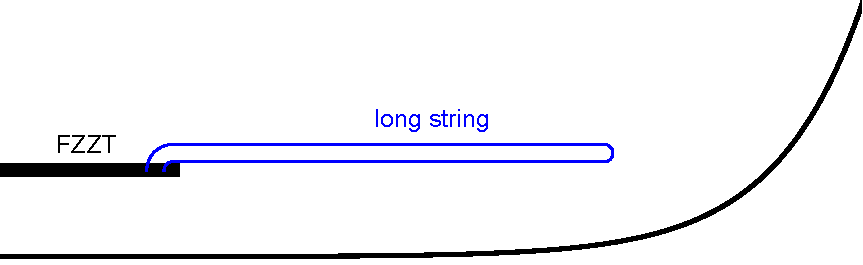
\includegraphics[width=.6\textwidth]{figures/longstring.pdf}
\caption{A high energy open string ending on an FZZT-brane in the asymptotic region, whose midpoint approaches the Liouville wall.}\label{fig:longstring}
\end{figure}


In the limit $s\to \infty$, the support of the FZZT$(s)$-brane recedes to the asymptotic region $X^1=-\infty$, and its backreaction on the closed string background diminishes. 
Nonetheless, we may consider an open string of energy $\omega$ in the limit
\ie{}
& s\to \infty, ~~~~\omega\to \infty,
\\
& \epsilon\equiv \omega - {2s\over \sqrt{\A'}}~~{\rm finite},
\fe
so that the midpoint of the string can reach the spatial region of finite coupling despite the ends of the string are stuck on the FZZT-brane in the asymptotic region. Such an open string is referred to as the {\it long string},\footnote{Maldacena, JHEP \textbf{09} (2005), 078 \cite{Maldacena:2005hi}. Note that this notion of long strings is unrelated to the one discussed in section \ref{sec:slstrfl}.} and $\epsilon$ will be referred to as the renormalized energy. 




Remarkably, the long string admits a precise dual description in an extension of the $c=1$ MQM, where one slightly relaxes the gauge-singlet constraint, as a state that transforms in the adjoint representation of the gauge group (Appendix \ref{app:longstr}). Similarly, a state consisting of $n$ long strings (and arbitrary closed string excitations) transforms in the $n$-th tensor power of the adjoint representation. As highly nontrivial tests of this proposal, the tree-level amplitude of a long string emitting a closed string, as well as the $2\to 2$ scattering amplitude of a pair of long strings, have been shown to numerically agree with the dual MQM description of the scattering amplitudes in the adjoint or bi-adjoint sectors in Balthazar, Rodriguez and Yin, JHEP \textbf{01} (2019), 173\cite{Balthazar:2018qdv}.






\newpage


\section{D-brane dynamics in type II superstring theory}

\subsection{Open+closed superstring perturbation theory}
\label{sec:openclosedpertsuper}

We now combine the recipes of Chapter \ref{sec:superscatter} and section \ref{sec:openclosedpert} to formulate the open+closed type II superstring perturbation theory. In the superconformal gauge, the superstring worldsheet is covered by holomorphic charts ${\cal U}_i$ that are parameterized by the super coordinates $(z_i, \theta_i)$ with superconformal transition maps on the overlap between charts as in (\ref{scatransfchar}), as well as their anti-holomorphic analog, the charts $\overline{\cal U}_i$ with the super coordinates $(\bar z_i, \bar\theta_i)$. When ${\cal U}_i$ and $\overline{\cal U}_i$ share a boundary component, we must introduce a transition map that accounts for the boundary condition, as follows.

Without loss of generality, we may assume that the chart ${\cal U}_i$ that meets the boundary is parameterized by $(z_i, \theta_i)$ with ${\rm Im}(z_i)> 0$, and similarly $\overline{\cal U}_i$ is parameterized by $(\bar z_i, \bar\theta_i)$ with ${\rm Im}(\bar z_i)< 0$. On their overlap, we demand the transition map to be
\ie\label{dryzztrans}
\bar z_i = z_i^*, ~~~~ \bar\theta_i = \pm \theta_i^*,
\fe
where $*$ acts as the usual complex conjugation on a complex parameter, and as a formal complex conjugation upon composition with superconformal maps. The data of the holomorphic and anti-holomorphic super coordinate charts subject to the boundary transition maps of the form (\ref{dryzztrans}), modulo the equivalence relation of superconformal diffeomorphism that preserve the boundary condition, define the notion of a {\it super Riemann surface with boundary} (BSRS). 

Note that in our definition of BSRS, the super coordinates on holomorphic and anti-holomorphic charts that do not meet at the boundary are a priori unrelated, and so the reduced space is not quite a Riemann surface with boundary. In particular, 
in the absence of boundary, the BSRS reduces to a holomorphic SRS $\mathfrak{C}$ together with an anti-holomorphic SRS $\overline{\mathfrak C'}$, whose supermoduli space is ${\mathfrak M}_{h,\epsilon_L}\times \overline{\mathfrak M}_{h,\epsilon_R}$, where $h$ is the genus and $\epsilon_L, \epsilon_R$ label the holomorphic and anti-holomorphic spin structures. More generally, with $b$ boundary components and $n_{\rm NS/R}$ the total number of holomorphic, anti-holomorphic, and boundary punctures of NS/R type, the supermoduli space of the BSRS has dimension $2d_e|d_o$, where 
\ie
& d_e = 6h-6 + 3b + n_{\rm NS} + n_{\rm R},
\\
& d_o = 4h-4 + 2b + n_{\rm NS} + {n_{\rm R}\over 2}.
\fe
The spin structure $\epsilon$ on the BSRS includes the choice of sign in (\ref{dryzztrans}) associated with each boundary component (this is the same sign as $\hat\eta$ appearing in (\ref{gbetagambdry}), (\ref{dpbryst})), as well as the choice of spinor field periodicity along the boundary circle (this amounts to restricting the boundary state (\ref{dpbryst}) to its (NS,NS) or (R,R) component). The latter is subject to the constraint that the total number of R type punctures and boundary states must be even. Therefore, for a given set of puncture types, the total number of distinct spin structures on the BSRS (with $b\geq 1$) is $2^{4h+2b-1}$. Note that while a boundary puncture of NS type does not affect the boundary spin structure, a boundary puncture of R type interpolates between boundary conditions of $+$ and $-$ spin structures, as is reflected in the cylinder modular crossing relations (\ref{dpabr}). Moreover, correlation functions of GSO-projected vertex operators are invariant under simultaneously flipping the spin structure assignments of all boundary components.

Generalizing (\ref{superamp}), the open+closed amplitude at genus $h$ with $b$ boundary components is given by
\ie\label{openclosedsupamp}
{\cal A}_{h, b}\left[\{V_i^c\}_{1\leq i\leq n}, \{V_j^o\}_{1\leq j\leq m}\right] = {\mathfrak N}_{h,n;b,m} \sum_\epsilon \int_{{\mathfrak G}_{h,n;b,m;\epsilon}} \Omega,
\fe
where $V_i^c$ and $V_j^o$ are closed and open string vertex operators. $\Omega$ is the integral form
\ie
\Omega = \left\langle e^{\cal B} \prod_{i=1}^n {\cal V}_i^c \prod_{j=1}^m {\cal V}_j^o \right\rangle_{{\mathfrak C}^o},
\fe
where ${\cal B}$ is defined analogously to (\ref{omegasupercorr}) with the appropriate even and odd moduli of the BSRS $\mathfrak{C}^o$ with $n$ bulk punctures, $m$ boundary punctures, and spin structure $\epsilon$. The integration contour ${\mathfrak G}_{h,n; b,m; \epsilon}$ is a codimension $d_e|0$ subspace of the supermoduli space of $\mathfrak{C}^o$ whose reduced space is the bosonic moduli space of the underlying Riemann surface with boundary $\Sigma$. Finally, the normalization factor ${\mathfrak N}_{h,n;b,m}$, generalizing (\ref{nhmsuperss}) and (\ref{nhbnmbos}), is determined by similar unitarity considerations to be
\ie\label{normopensup}
{\mathfrak N}_{h,n;b,m} = { i^{3h-3+n} e^{{3\over 2} (b+{m\over 2}) {\pi i\over 2}} \over 2^{2h+b}},
\fe
provided that we adopt the same normalization of the closed and open superstring vertex operators as in (\ref{vvnormvonv}) and (\ref{vvopennorm}).

For explicit computations, it is typically more convenient to adopt the PCO formalism, in which the open+closed superstring amplitude is expressed as
\ie\label{openclosedsupamppco}
{\cal A}_{h, b}\left[\{V_i^c\}_{1\leq i\leq n}, \{V_j^o\}_{1\leq j\leq m}\right] = {\mathfrak N}_{h,n;b,m} \int_{\cal S} \wt \Omega,
\fe
where ${\cal S}$ is a suitable contour in the fiber bundle $\pi:{\cal Y}_{h,n;b,m}\to {\cal M}_{h,n;b,m}$, whose fiber is parameterized by the position of $d_o$ PCOs and the choice of the spin structure $\epsilon$ on the Riemann surface with boundary $\Sigma$. The PCOs may be either holomorphic, anti-holomorphic, or on the boundary. The differential form $\wt \Omega$ can be written as
\ie\label{wtompcoop}
\wt \Omega = \left\langle e^{\pi^*\cal B} \prod_{a=1}^{d_o} \left[ {\cal X}(z_a) - d\xi(\xi_a) \right] \prod_{i=1}^n {\cal V}_i^c \prod_{j=1}^m {\cal V}_j^o \right\rangle_{\Sigma,\epsilon}
\fe
when the PCOs are either holomorphic or at the boundary. The generalization of (\ref{wtompcoop}) to the case where some of the PCOs are chosen to be anti-holomorphic is obvious. 

The PCO contour ${\cal S}$ can be constructed similarly to the closed superstring case described in section \ref{sec:verticalpco}. Namely, on a patch of the moduli space ${\cal M}_{h,n;b,m}$, ${\cal S}$ is specified by the choice of PCO coordinates $z_1, \cdots, z_{d_o}$ for each of the $2^{4h+2b}$ spin structures on $\Sigma$, arranged so as to avoid spurious singularities. The mismatch of the PCO coordinates between the moduli patches is then corrected by vertical integration.

Our normalization convention for the ghost and matter CFT correlators on the disc with D$p$-brane boundary condition are
\ie\label{discnormsup}
& \left\langle c(z_1) c(z_2) c(z_3) \right\rangle_{bc,D^2} = z_{12} z_{13} z_{23},
~~~~ \left\langle \delta(\C(z_1)) \delta(\C(z_2)) \right\rangle_{bc,D^2} = {1\over z_{12}},
\\
& \left\langle e^{ik_\parallel\cdot X(z, \bar z)} \right\rangle_{{\rm m},D^2} = i (2\pi)^{p+1} \delta^{p+1}(k_\parallel) g_s^{-1} K_{D^2},
\fe
where $K_{D^2}$ is proportional to the normalization constant ${\cal N}_{{\rm D}p,{\rm NSNS}}$ (\ref{ndnsnsrrres}) appearing in the NSNS component of the D$p$-brane boundary state (\ref{nsdryst}). Their precise relation is determined through the cylinder modular crossing relation (\ref{dpabr}),
\ie\label{ndtwosup}
K_{D^2} = i \sqrt{8\pi \over \A'} {\cal N}_{{\rm D}p,{\rm NSNS}}.
\fe
where the factor $\sqrt{8\pi \over \A'}$ arises due to our normalization convention of the sphere correlator. The overall sign of $K_{D^2}$ in (\ref{ndtwosup}) is fixed by the reality of the open string coupling $g_o$ below.
For instance, the vertex operator of a massless NS gauge boson on a BPS D$p$-brane is
\ie\label{vasupe}
{\cal V}_A^{(-1)}(k_\parallel, e) = - e^{-{3\pi i\over 8}} g_o c\, e^{-\phi} e_\mu \psi^\mu \vdots e^{ik_\parallel \cdot X} \vdots,
\fe
where $k_\parallel^2=k_\parallel\cdot e=0$. The normalization condition (\ref{vvopennorm}) then determines the open string coupling $g_o$ appearing in (\ref{vasupe}) in terms of $g_s$ via
\ie\label{gsgosup}
g_s = - e^{-{3\pi i \over 4}} g_o^2 {K_{D^2}\over K_o} =  {g_o^2\over 4\sqrt{\pi}} (2\pi \sqrt{\A'})^{5-p}.
\fe


\subsection{Disc open string amplitudes}

The tree-level amplitude of $n_{\rm NS}$ bosonic and $n_{\rm R}$ fermionic open superstring states involves the insertion of $d_o = n_{\rm NS} + {n_{\rm R}\over 2}-2$ PCOs, which may be arranged to be on the boundary of the disc and moreover coincide with a subset of the open string vertex operators. We will illustrate this with the disc amplitudes of massless gauge bosons on a stack of $N$ BPS D$p$-branes. The relevant $(-1)$-picture vertex operator is
\ie
{\cal V}_A^{(-1)}(k_\parallel, e, a) = {\cal V}_A^{(-1)}(k_\parallel, e) \otimes t^a,
\fe
where ${\cal V}_A^{(-1)}(k_\parallel, e)$ is defined as in (\ref{vasupe}), and the Chan-Paton factors $t^a$ are a basis of $N\times N$ Hermitian matrices normalized with ${\rm tr}(t^at^b)=\delta^{ab}$. The corresponding picture-raised vertex operator is
\ie
{\cal V}_A^{(0)}(k_\parallel, e, a) = - e^{-{3\pi i\over 8}} g_o c {e_\mu\over \sqrt{2\A'}} \vdots \left( i \partial X^\mu + \A' k_\parallel\cdot \psi \psi^\mu \right) e^{ik_\parallel\cdot X}\vdots  \otimes t^a + ({\rm term ~involving} ~\eta),
\fe
where we have used the doubling trick notation, and the term involving $\eta$ will drop out of the disc amplitudes of interest.


As all vertex operators are GSO-projected, the disc correlation function is insensitive to the choice of boundary spin structure $\hat\eta=\pm$. Moreover, the sum over $\hat\eta=\pm$ cancels against a factor of ${1\over 2}$ from the normalization constant (\ref{normopensup}). The disc amplitude of 3 gauge bosons is therefore
\ie\label{discuspthr}
&{\cal A}_{0,1}\left[\{V_A(k_i,e_i,a_i)\}_{1\leq i\leq 3}\right] 
\\
&= e^{{3\pi i\over 8}}  \left\langle {\cal V}_A^{(-1)}(k_1, e_1,a_1)(y_1) {\cal V}_A^{(-1)}(k_2, e_2,a_2)(y_2){\cal V}_A^{(0)}(k_3, e_3,a_3)(y_3) \right\rangle_{D^2} + (2\leftrightarrow 3)
\\
&= e^{-{3\pi i\over 4}} g_o^3 \left\langle  e_1\cdot\psi \vdots e^{ik_1\cdot X}\vdots (y_1)  e_2\cdot\psi \vdots e^{ik_2\cdot X}\vdots (y_2)  {e_{3\mu}\over \sqrt{2\A'}} \vdots (i \partial X^\mu + \A' k_3\cdot \psi \psi^\mu ) e^{ik_3\cdot X}\vdots (y_3) \right\rangle_{{\rm m},D^2} 
\\
&~~~\times {\rm tr}\left(\lambda^{a_1} \lambda^{a_2} \lambda^{a_3} \right) + (2\leftrightarrow 3).
\fe
The matter correlator $\langle \cdots \rangle_{{\rm m},D^2}$ above evaluates to
\ie
- i (2\pi)^{p+1} \delta^{p+1}\Big( \sum_{i=1}^3 k_i \Big) g_s^{-1} K_{D^2} e_{1\mu} e_{2\nu} e_{3\rho} \sqrt{\A'\over 2} \left[ - {\eta^{\mu\nu}\over y_{12}}\left( {k_1^\rho\over y_{13}}+{k_2^\rho\over y_{23}} \right) + {- k_3^\mu \eta^{\nu\rho} + k_3^\nu \eta^{\mu\rho}\over y_{13} y_{23}} \right] .
\fe
After simplification using the kinematic constraints and the relation (\ref{gsgosup}), and factoring out $i (2\pi)^{p+1} \delta^{p+1}( \sum k_i )$, the reduced disc amplitude of 3 gauge boson can be expressed as
\ie\label{aredthrop}
\widehat{\cal A}_{0,1}\left[\{V_A(k_i,e_i,a_i)\}_{1\leq i\leq 3}\right] 
&= {g_o\over \sqrt{2\A'}} {\rm tr} \left(\lambda^{a_1} [\lambda^{a_2}, \lambda^{a_3}]\right)  \prod_{i=1}^3 e_{i,\mu_i} 
\big(  \eta^{\nu_1\nu_2}k_1^{\nu_3}  + \eta^{\nu_2\nu_3} k_2^{\nu_1} + \eta^{\nu_1\nu_3} k_3^{\nu_2} \big).
\fe
This agrees with the on-shell 3-point vertex of a $U(N)$ effective gauge theory, whose action is of the form
\ie\label{assupopeff}
S_{\rm eff}[A_\mu,\cdots] = \int d^{p+1}x \left[ - {1\over 4g_{\rm YM}^2} {\rm tr} (F_{\mu\nu} F^{\mu\nu}) + \cdots \right],
\fe
where $F_{\mu\nu}\equiv \partial_\mu A_\nu - \partial_\nu A_\mu - i[A_\mu,A_\nu]$ is the non-Abelian gauge field strength, and the gauge coupling $g_{\rm YM}$ is identified as
\ie\label{gymgobos}
g_{\rm YM} = 2^{-{3\over 2}} {g_o\over \sqrt{\A'}}.
\fe
Note that the absence of higher powers of momentum on the RHS of (\ref{aredthrop}) implies the absence of nontrivial order $\A'$ corrections to the Lagrangian density of (\ref{assupopeff}), e.g. couplings of the form ${\rm Tr} (F_\mu{}^\nu F_\nu{}^\rho F_\rho{}^\mu)$. This property can also be understood as a consequence of the Ward identities on the open string amplitudes associated with the 16 supersymmetries preserved by the D$p$-branes.


Next, let us consider the disc amplitude of 4 gauge bosons,
\ie\label{discfoursup}
&{\cal A}_{0,1}\left[\{V_A(k_i,e_i,a_i)\}_{1\leq i\leq 4}\right] 
= e^{{3\pi i\over 4}} \bigg\langle{\cal V}_A^{(-1)}(k_1, e_1)(\infty) {\cal V}_A^{(-1)}(k_2, e_2)(1) {\cal V}_A^{(0)}(k_3, e_3)(0)
\\
&~~~\times  \int_0^1 dy_4 (-b_{-1}) {\cal V}_A^{(0)}(k_4, e_4)(y_4) \bigg\rangle_{D^2}  {\rm tr} \left(\lambda^{a_1}\lambda^{a_2} \lambda^{a_4} \lambda^{a_3}\right)  + ({\rm permutations~on~}2,3,4).
\fe
Here we have set $y_1=\infty$, $y_2=1$, $y_3=0$, and have split the $y_4$-integral over the three segments, $y_4<0$, $0<y_4<1$ and $y_4>1$, where the relevant disc correlators come with different ordering of the Chan-Paton factors in the trace. 
%\ie{}
%&= i (2\pi)^{p+1} \delta^{p+1} g_s^{-1} K_{D^2} \Big(\sum_{i=1}^4 k_i \Big) {1\over 2\A'} y^{2\A' k_1\cdot k_4} (1-y)^{2\A' k_2\cdot k_4} \Bigg\{ -e_1\cdot e_2 \bigg[ \A'^2 \left( -k_3\cdot k_4 e_3\cdot e_4 + k_3\cdot e_4 k_4\cdot e_3 \right) 
%\\
%&~~~~~~~~~~~~~~~~ + \A'^2 (k_2\cdot e_3 + y k_4\cdot e_3) \left( {k_1\cdot e_4\over y} + {k_2\cdot e_4\over y-1} \right) + {\A'\over 2} e_3\cdot e_4 \bigg]
%\\
%&~~~ + \A'^2 \bigg[ \left( e_2\cdot k_3 e_1\cdot e_3 - e_1\cdot k_3 e_2\cdot e_3 \right) \left( {k_1\cdot e_4\over y} + {k_2\cdot e_4\over y-1} \right)
%\\
%&~~~~~~~~~~~~ + \left( e_2\cdot k_4 e_1\cdot e_4 - e_1\cdot k_4 e_2\cdot e_4 \right) (k_2\cdot e_3 + y k_4\cdot e_3)  \bigg]
%\\
%&~~~ + {\A'^2 \over y-1} \bigg( e_1 \cdot k_3 e_2\cdot k_4 e_3\cdot e_4 + e_1\cdot e_3 e_2\cdot e_4 k_3\cdot k_4 - e_1\cdot e_3 e_2\cdot k_4 e_4\cdot k_3 - e_1\cdot k_3 e_2\cdot e_4 e_3\cdot k_4 \bigg)
%\\
%&~~~ - {\A'^2 \over y} \bigg( e_1 \cdot k_4 e_2\cdot k_3 e_3\cdot e_4 + e_1\cdot e_4 e_2\cdot e_3 k_3\cdot k_4 - e_1\cdot e_4 e_2\cdot k_3 e_3\cdot k_4 - e_1\cdot k_4 e_2\cdot e_3 e_4\cdot k_3 \bigg) \Bigg\}
%\fe
After a somewhat tedious evaluation of the disc correlator and the $y_4$-integral, the result for the 4-point reduced amplitude can be expressed as
\ie\label{redufouraop}
&\widehat {\cal A}_{0,1}\left[\{V_A(k_i,e_i,a_i)\}_{1\leq i\leq 4}\right] 
\\
&= - g_o^2 \A' K^{{\rm NS},o}(\{k_i,e_i\}) \left[ {\Gamma(-\A' s) \Gamma(-\A' t)\over \Gamma(1-\A's -\A' t)} {\rm Tr}(\lambda^{a_1}\lambda^{a_2}\lambda^{a_3}\lambda^{a_4}) + ({\rm permutations~on~2,3,4}) \right],
\fe
where 
\ie
K^{{\rm NS},o}(\{k_i,e_i\}) \equiv t_8^{\mu_1\nu_1\cdots \mu_4\nu_4} \prod_{i=1}^4 e_{i\mu_i} k_{i\nu_i},
\fe
with the Lorentz invariant tensor $t_8$ defined in (\ref{teightdef}).

The first term in the bracket on the RHS of (\ref{redufouraop}) exhibits poles in $s$ and $t$ that correspond to the exchange of on-shell open string states in the $12\to 34$ and $23\to 41$ channels respectively. It is illuminating to inspect the $\A'$ or momentum expansion, using
\ie\label{gammstexpa}
{\Gamma(-\A' s) \Gamma(-\A' t)\over \Gamma(1-\A's -\A' t)} = {1\over \A'^2 st} - {\pi^2\over 6} + {\cal O}(\A'^2).
\fe
The leading term on the RHS produces none other than the tree-level 4-point amplitude of Yang-Mills theory, as expected from the effective action (\ref{assupopeff}). The second term on the RHS of (\ref{gammstexpa}) indicates an order $\A'^2$ correction to (\ref{assupopeff}), of the form
\ie\label{seffteightf}
S_{\rm eff}|_{\A'^2} = {\pi^2 \A'^2 \over 48 g_{\rm YM}^2} \int d^{p+1}x \left[ t_8^{\mu_1\nu_1\cdots \mu_4\nu_4} {\rm tr} (F_{\mu_1\nu_1} F_{\mu_2\nu_2} F_{\mu_3\nu_3} F_{\mu_4\nu_4}) + \cdots \right],
\fe
where $\cdots$ stands for other couplings involving the massless scalar fields and gauginos that are related by supersymmetry. We will see in section \ref{sec:dbraneeffii} and \ref{sec:nonabeldbrane} that the correction (\ref{seffteightf}) is part of the Born-Infeld effective action that is valid at finite field strength.


\subsection{Disc open+closed string amplitudes}
\label{sec:disccs}

We now consider a simple example of a disc amplitude that involves open and closed string states. A massless (R,R) closed string state is represented by the vertex operator ${\cal V}^{(-{1\over 2},-{1\over 2})}(k,f)= c\wt c V_{\rm RR}(k,f)$, where
\ie
V_{\rm RR}(k,f) = g_s f^{\A\widehat\A} j_\A \wt j_{\widehat\A} \vdots e^{ik\cdot X}\vdots .
\fe
The polarization tensor $f^{\A\widehat\A}$ obeys (\ref{kgammaspaeom}) and is related to the RR field strength as in (\ref{falphaind}). $j_\A$, $\wt j_{\widehat\A}$ are the spacetime supersymmetry currents (\ref{stsusycurrents}). The disc amplitude with a massless (R,R) closed string state and a massless NS open string state on a D$p$-brane located at transverse coordinate $x_\perp$ is
\ie\label{coamprr}
& {\cal A}_{0,1}\left[ V_{\rm RR}(k,f), V_A(k'_\parallel,e)\right] = e^{\pi i \over 8} \left\langle {\cal V}^{(-{1\over 2},-{1\over 2})}(k,f)(z,\bar z) {\cal V}_A^{(-1)}(k_\parallel', e)(y)  \right\rangle_{D^2}
\\
&= i(2\pi)^{p+1} \delta^{p+1}(k_\parallel+k'_\parallel) e^{ik_\perp\cdot x_\perp} (-i){g_s \over g_o\A'}  f^{\A\widehat\A} e_\mu \left\langle c\wt c j_\A \wt j_{\widehat\A}(z, \bar z) c e^{-\phi} \psi^\mu(y) \right\rangle_{{\rm gh}, \psi, D^2},
\fe
where we have written $k^\mu = k_\parallel^\mu + k_\perp^\mu$, with $k_\parallel$ and $k_\perp$ being the components of the closed string momentum parallel and perpendicular to the D$p$-brane, respectively. The polarization vector $e_\mu$ may either be taken to be parallel to the D$p$-brane, corresponding to the polarization of the gauge boson subject to the transversality condition $k_\parallel'\cdot e =0$, or be perpendicular to the D$p$-brane, corresponding to the collective coordinate of the D$p$-brane.

The relevant spin field correlator can be calculated using the doubling relation (\ref{doublingtrickii}) and the OPE (\ref{susyope}), yielding
\ie
\left\langle c\wt c j_\A \wt j_{\widehat\A}(z, \bar z) c e^{-\phi} \psi^\mu(y) \right\rangle_{{\rm gh}, \psi, D^2} 
= - {1\over \sqrt{2}} (\Gamma^\mu)_{\A\B} ((\B^{p+1}\cdots \B^9)^{-1})_{\widehat\A}{}^\B.
\fe
In terms of the polarization tensor $f^{\mu_1\cdots\mu_p}$ (\ref{falphaind}) associated with the $p$-form RR field strength, for $e$ parallel to the D$p$-brane, the amplitude (\ref{coamprr}) is proportional to $e_\mu f_{\mu_1\cdots\mu_p} \epsilon^{\mu\mu_1\cdots\mu_{p}}$, where $\epsilon$ is the constant anti-symmetric tensor in the $p+1$ dimensions along the D$p$ world volume. This amounts to an effective coupling of the Chern-Simons form (up to a normalization constant)
\ie\label{afdiscc}
\int_{{\rm D}p} A\wedge F_p ,
\fe
where $A$ is the 1-form potential on the D$p$-brane, and $F_p=dC_{p-1}$ is the $p$-form field strength associated with the $(p-1)$-form RR potential $C_{p-1}$, restricted to the D$p$-brane world volume.

For $e_\mu = \delta_{\mu i}$ perpendicular to the D$p$-brane ($i=p+1,\cdots,9$), on the other hand, the amplitude (\ref{coamprr}) is proportional to $f_{01\cdots p i }$, which amounts to an effective coupling (up to a normalization constant)
\ie\label{fdeltxdpc}
\int_{{\rm D}p} d^{p+1} x \, (F_{p+2})_{01\cdots p i} \Delta X^i,
\fe
where $\Delta X^i$ is the displacement of the D$p$-brane in the $X^i$ direction. We will see in section \ref{sec:dbraneeffii} that this is in fact part of the brane coupling to the RR $(p+1)$-form potential $C_{p+1}$, and in particular indicates that the D$p$-brane is charged with respect to $C_{p+1}$.




\subsection{Cylinder amplitudes}
\label{sec:cyltypeii}

The open string 1-loop amplitude, associated with the cylinder topology, can also be interpreted as the amplitude of a tree-level emission and absorption of a closed string by the D-brane. As the simplest example, the cylinder vacuum amplitude, generalizing the bosonic string expression (\ref{cylvacboss}), is
\ie\label{cylsupgen}
{\cal A}_{0,2} = -{i\over 2} \sum_{\epsilon_1,\epsilon_2=\pm} \int_0^\infty {dt\over 2t} \left\langle bc \right\rangle_{C^2(t), (\epsilon_1,\epsilon_2)},
\fe
where the spin structure of the cylinder, up to a simultaneous flip of the boundary spin structures, can be identified with the holomorphic spin structure on a torus via the doubling trick, specified by the periodicity condition $(\epsilon_1, \epsilon_2) = (\pm, \pm)$ on the holomorphic worldsheet spinor fields around the spatial and Euclidean time circles of the torus. The cylinder partition functions with $bc$ ghost insertion and various spin structure assignments can be expressed as\footnote{Note that the trace expression for the cylinder partition function involves a different sign convention from its bosonic string analog (\ref{cylvacboss}).}
\ie\label{epsopensupcyl}
-i \left\langle bc \right\rangle_{C^2(t), (\epsilon_1,\epsilon_2)} = -\epsilon_1 {\rm Tr}_{{\cal H}^o_{\epsilon_1}} (-)^{N_{bc}+N_{\B\C}} (-\epsilon_2)^F b_0 c_0 e^{- 2\pi t L_0} ,
\fe
where ${\cal H}_-^o$ and ${\cal H}_+^o$ are the space of NS and R sector states on the strip, in the $-1$ and $-{1\over 2}$ picture respectively. The trace on the RHS in the $(+,-)$ spin structure case involves a sum over degenerate Ramond ground states of the $\B\C$ system with alternating signs, and should be regularized as in (\ref{twistchareg}), (\ref{parttwsithir}). The $(+,+)$ spin structure contribution, on the other hand, suffers from an ``$\infty\times 0$'' ambiguity similar to the one mentioned below (\ref{oddscont}); in this case, there isn't an obvious extension of the $n$-punctured cylinder amplitude from $n\geq 1$ (as formulated in section \ref{sec:openclosedpertsuper}) to the $n=0$ case. This ambiguity can be overcome either by working in the lightcone gauge, or by considering the cylinder amplitude with at least one boundary vertex operator corresponding to the collective coordinate of the D-brane. The end result is that the $(+,+)$ spin structure contribution vanishes.\footnote{The vanishing of the $(+,+)$ partition function can also be understood through the cancellation between states of opposite worldsheet fermion parity due to the worldsheet supersymmetry preserved by the Ramond boundary condition on the strip.}

The cylinder vacuum amplitude between a pair of D-branes described by boundary conditions $B_1$ and $B_2$, generalizing the bosonic string case (\ref{aonetwdd}), can be written as
\ie\label{cylampint}
& {\cal A}_{0,2}^{(12)} = {\cal A}_{0,2}^{(12),{\rm NSNS}} + {\cal A}_{0,2}^{(12),{\rm RR}},
\\
& {\cal A}_{0,2}^{(12),{\rm NSNS}} = {1\over 2} \int_0^\infty {dt\over t} \big( {\rm Tr}_{{\cal H}^{\rm NS}_{B_1B_2}} - {\rm Tr}_{{\cal H}^{\rm R}_{B_1B_2}} \big) (-)^{N_{bc}+N_{\B\C}} b_0 c_0 e^{- 2\pi t L_0} ,
\\
& {\cal A}_{0,2}^{(12),{\rm RR}} = {1\over 2} \int_0^\infty {dt\over t} \big( {\rm Tr}_{{\cal H}^{\rm NS}_{B_1B_2}} - {\rm Tr}_{{\cal H}^{\rm R}_{B_1B_2}} \big) (-)^{N_{bc}+N_{\B\C}+F} b_0 c_0 e^{- 2\pi t L_0} .
\fe
In comparison to (\ref{cylsupgen}), an overall factor of 2 is included to account for open strings of both orientations, corresponding to states in ${\cal H}_{B_1B_2}$ as well as ${\cal H}_{B_2B_1}$. The minus sign of the Ramond sector ${\cal H}_{B_1B_2}^R$ contribution, as dictated by the modular invariance of (\ref{epsopensupcyl}), can be interpreted as due to the fermionic spacetime statistics of the corresponding open string fields. ${\cal A}_{0,2}^{(12),{\rm NSNS}}$ and ${\cal A}_{0,2}^{(12),{\rm RR}}$ can be interpreted as the exchange amplitude of a closed string in the (NS,NS) and (R,R) sector respectively.

Now suppose $B_1, B_2$ are a pair of D$p$-branes separated by $\Delta x_\perp$ in their transverse coordinates. ${\cal A}_{0,2}^{(12),{\rm NSNS}}$ is evaluated by tracing over the open string states as
\ie\label{zcylminu}
&{\cal A}_{0,2}^{(12),{\rm NSNS}} = {i V_{p+1} \over 2} \int_0^\infty {dt\over t}  (8\pi^2 \A' t)^{-{p+1\over 2}} e^{- t {(\Delta x_\perp)^2\over 2\pi \A'}} (\eta(it))^{-8} \left[ \left( {\theta_3(0|it)\over \eta(it)} \right)^{4} - \left( {\theta_2(0|it)\over \eta(it)} \right)^{4} \right],
\fe
where we have used ${\theta_3(0|it)\over \eta(it)} = q^{-{1\over 24}}\prod_{n=0}^\infty (1+q^{n+{1\over 2}})^2$ and ${\theta_2(0|it)\over \eta(it)} = 2q^{{1\over 12}}\prod_{n=1}^\infty (1+q^n)^2$, $q\equiv e^{-2\pi t}$. 
Using the modular property of Jacobi theta functions, we can rewrite (\ref{zcylminu}) as
\ie{}
{\cal A}_{0,2}^{(12),{\rm NSNS}} &=  {i V_{p+1} \over 2} (8\pi^2 \A' )^{-{p+1\over 2}}  \int_0^\infty dt\, t^{5-p\over 2} e^{- t {(\Delta x_\perp)^2\over 2\pi \A'}} (\eta(i/t))^{-8} \left[ \left( {\theta_3(0|i/t)\over \eta(i/t)} \right)^{4} - \left( {\theta_4(0|i/t)\over \eta(i/t)} \right)^{4} \right]
\\
%&=  {i V_{p+1} \over 2} (8\pi^2 \A' )^{-{p+1\over 2}}  \int_0^\infty dt\, t^{5-p\over 2} e^{- t {(\Delta x)^2\over 2\pi \A'}} (\eta(i/t))^{-8}e^{{1\over 6}{2\pi\over t}} \left[ \prod_{n=0}^\infty (1+e^{-(n+{1\over 2}){2\pi\over t}})^8 - \prod_{n=0}^\infty (1-e^{-(n+{1\over 2}){2\pi\over t}})^8 \right]
%\\
&=  {i V_{p+1} \over 2} (8\pi^2 \A' )^{-{p+1\over 2}}  \int_0^\infty dt\, t^{5-p\over 2} e^{- t {(\Delta x_\perp)^2\over 2\pi \A'}} \left[ 16 + {\cal O}(e^{-{2\pi\over t}}) \right].
\fe
${\cal A}_{0,2}^{(12),{\rm NSNS}}/(i V_{p+1})$ can be interpreted as the leading contribution to the energy density due to the exchange of (NS,NS) closed string modes between the pair of D$p$-branes. In particular, the graviton and dilaton exchange amplitude (from the term ``16'' in the bracket) contributes to an attractive Newtonian potential proportional to $|\Delta x_\perp|^{p-7}$. The terms of order $e^{-{2\pi\over t}}$ in the bracket correspond to the exchange of massive (NS,NS) closed string modes.

${\cal A}_{0,2}^{(12),{\rm RR}}$ can be evaluated similarly. By the same identity of Jacobi theta functions as seen in the cancellation of (\ref{zodd}), one finds
\ie\label{arrnsns}
{\cal A}_{0,2}^{(12),{\rm RR}} = -{\cal A}_{0,2}^{(12),{\rm NSNS}}.
\fe
That is, the exchange amplitude of (R,R) closed string modes exactly cancels that of (NS,NS) closed string modes, and so the potential between a pair of parallel D$p$-brane vanishes. This cancellation can be understood as a consequence of the supersymmetry preserved by the parallel D$p$-branes. It also indicates that the D-branes are charged with respect to the massless (R,R) fields, which exchange gives rise to a repulsive potential that cancels the Newtonian attraction due to the graviton and dilaton exchange.

We could alternatively consider the system of a D$p$-brane and a parallel anti-D$p$-brane, separated by $\Delta x_\perp$. In this case, the cylinder vacuum amplitude is computed by (\ref{zcylminu}) where the open string states are now subject to the opposite GSO projection, i.e. $(-)^F$ acts with the opposite sign on the same space of states on the strip. This leads to the same result (\ref{zcylminu}) for ${\cal A}_{0,2}^{(12),{\rm NSNS}}$, but now ${\cal A}_{0,2}^{(12),{\rm RR}}$ acquires the opposite sign as (\ref{arrnsns}). That is, the anti-D$p$-brane carries the opposite (R,R) charge as the D$p$-brane, in which case the exchange of RR fields gives an identical contribution to the attractive potential as the graviton/dilaton exchange.









\subsection{BPS D-brane effective action}
\label{sec:dbraneeffii}

%The BPS D$p$-brane in type II string theory admit an effective action that couples the massless open string fields to the closed string background. 

\subsubsection{Supersymmetry and $\kappa$ symmetry}

We begin by considering a BPS D$p$-brane in the 10-dimensional Minkowskian spacetime, in the absence of nontrivial closed string excitations, and construct an effective action that is invariant under the super-Poincar\'e symmetry with 32 supercharges. Similarly to that of the Green-Schwarz action of the superstring (section \ref{sec:gssupact}), the ${1\over 2}$-BPS nature of the D$p$-brane is such that the 32 supersymmetries are realized nonlinearly in an effective theory of 16 Goldstinos (which can be identified with the gauginos). 

As in section \ref{sec:dbraneeff}, we adopt an arbitrary world volume coordinate system $\xi^a$ ($a=0,\cdots,p$) and parameterize the D-brane configuration in the spacetime with the embedding coordinate fields $X^\mu(\xi)$, $\mu=0,\cdots,9$. In addition, we have a $U(1)$ gauge field $A_a$ and fermion fields $\theta\equiv(\theta^\A, \theta^{\widehat\A})$ that transform in a pair of Majorana-Weyl representations of $so(1,9)$ with the same (opposite) chirality in the type IIB (IIA) case. %In the IIB case, we will typically suppress the label for the two of M-W spinors, and in various formulae an explicit sum over the two copies is understood. 
Under the spacetime supersymmetry generated by a 32-component spinor parameter $\epsilon\equiv(\epsilon^\A, \epsilon^{\widehat\A})$, the fields $X^\mu$ and $\theta$ transform according to
\ie\label{dbrandusytrans}
\delta_\epsilon \theta = \epsilon,~~~~ \delta_\epsilon X^\mu = \overline\epsilon \Gamma^\mu \theta.
\fe
Invariant under (\ref{dbrandusytrans}) are the Noether currents $\partial_a\theta$ associated with supersymmetry and 
\ie
\Pi_a^\mu = \partial_a X^\mu - \overline\theta \Gamma^\mu \partial_a \theta,~~~~\Pi\equiv \Pi_a d\xi^a,
\fe
associated with the spacetime momentum. A supersymmetry invariant that generalizes the notion of the induced metric (\ref{inducedmetricbos}) in the bosonic case is
\ie
{\cal G}_{ab} = \eta_{\mu\nu} \Pi_a^\mu \Pi_b^\nu.
\fe
A supersymmetry-invariant generalization of the gauge-invariant combination (\ref{bplusf}), in the absence of background $B$-field, turns out to be 
\ie{}
& {\cal F}_{ab} = {\cal B}_{ab} + 2\pi \A' F_{ab} ,
\\
& {\cal B} \equiv {1\over 2}{\cal B}_{ab} d\xi^a d\xi^b = \overline\theta \Gamma_{11} \Gamma_\mu d\theta \wedge \left( dX^\mu + {1\over 2} \overline\theta \Gamma^\mu d \theta \right).
\fe
Here $F_{ab}$ is the ordinary field strength of the gauge potential $A_a$, and ${\cal B}_{ab}$ is the pullback of super-$B$-field of the Minkowskian spacetime (\ref{supbfiex}) to the D$p$-brane world volume.\footnote{Here a different phase convention for the components of $\theta$ is adopted in comparison to that of the Green-Schwarz action considered in section \ref{sec:gsgenbkgrd}.}
The supersymmetry variation of ${\cal B}$,
\ie
\delta_\epsilon {\cal B} = \overline\epsilon \Gamma_{11} \Gamma_\mu d\theta \left( dX^\mu + {1\over 2} \overline\theta \Gamma^\mu d \theta \right) - (\overline\theta \Gamma_{11} \Gamma_\mu d\theta) ( \overline\epsilon \Gamma^\mu d\theta ),
\fe
can be expressed by Fierz rearrangement as a total derivative $-d (\delta_\epsilon A)$, where $\delta_\epsilon A$ is the supersymmetry variation of the gauge potential 1-form,
\ie\label{deltaagau}
2\pi \A' \delta_\epsilon A = ( \overline\epsilon \Gamma_{11} \Gamma_\mu \theta)  dX^\mu + {1\over 6} \left[  (\overline\epsilon \Gamma_{11} \Gamma_\mu \theta) ( \overline\theta \Gamma^\mu d\theta ) +  ( \overline\epsilon \Gamma^\mu \theta )  (\overline\theta \Gamma_{11} \Gamma_\mu d\theta) \right],
\fe
and consequently ${\cal F}_{ab}$ is supersymmetry invariant.

Analogously to the construction of the Green-Schwarz action, one should further introduce a fermionic $\kappa$ gauge symmetry to remove half of the degrees of freedom of the 32-component fermion field $\theta$. An effective action of the BPS D$p$-brane in type II superstring theory that extends the Born-Infeld action (\ref{dpdbibos}) of the bosonic string case, and is invariant under both supersymmetry and the $\kappa$ gauge symmetry, turns out to be\footnote{Aganagic, Popescu, Schwarz, Nucl. Phys. B \textbf{495} (1997), 99 \cite{Aganagic:1996nn}.}
\ie\label{susydbi}
S = - T_p \int d^{p+1}\xi \sqrt{-\det ({\cal G}_{ab} + {\cal F}_{ab})} + \int \Omega_{p+1},
\fe
where $\Omega_{p+1}$ is a certain supersymmetry-invariant $(p+1)$-form known as the Wess-Zumino term. Assuming that the D$p$-brane world volume is the boundary of a $(p+2)$-dimensional space ${\cal V}$, and that the world volume fields $(X, A, \theta)$ can be extended differentiably to ${\cal V}$, the Wess-Zumino term can be defined as
\ie
\int_{\partial {\cal V}} \Omega_{p+1} = \int_{\cal V} I_{p+2},
\fe
where
\ie
I_{p+2}\equiv d\Omega_{p+1} = (-)^{p+1} d\overline\theta \, W_p \, d\theta.
\fe
Here $W_p$ is a spinor-matrix valued $p$-form, given by the generating formula
\ie\label{sumwpsi}
& \sum_{{\rm even} ~p} W_p = e^{\cal F} \sum_{n\geq 0} {1\over (2n)!} \Gamma_{11}^{n+1}(\Pi^\mu \Gamma_\mu)^{2n}~~~~({\rm IIA}),
\\
& \sum_{{\rm odd} ~p} W_p = e^{\cal F} \sum_{n\geq 0} {1\over (2n+1)!} \sigma_3^n \sigma_1 (\Pi^\mu \Gamma_\mu)^{2n+1} ~~~~({\rm IIB}),
\fe
where in the type IIB case $\sigma_1$ and $\sigma_3$ are the Pauli matrices, with $\theta$ viewed a doublet of Majorana-Weyl spinors. 

The $\kappa$-symmetry variations of the world volume fields that leave the action (\ref{susydbi}) invariant are \footnote{It follows from (\ref{kappaax}) that 
\ie{}
& \delta_\kappa \Pi^\mu_a = - 2 \delta_\kappa\bar\theta \Gamma^\mu \partial_a \theta, ~~~ \delta_\kappa {\cal G}_{ab} = - 2\delta_\kappa\bar\theta \Gamma_\mu (\Pi^\mu_a \partial_b+\Pi^\mu_b \partial_a) \theta,\\
& \delta_\kappa {\cal F}_{ab} = 2\delta_\kappa\bar\theta \Gamma_{11}\Gamma_\mu (\Pi^\mu_a \partial_b-\Pi^\mu_b \partial_a) \theta.
\fe 
One can then determine $\delta_\kappa\theta$ by requiring the variation of the Born-Infeld term in (\ref{susydbi}) to cancel against the variation of the Wess-Zumino term. }
\ie\label{kappaax}
& \delta_\kappa X^\mu = \overline\theta\Gamma^\mu \delta_\kappa\theta,
\\
&2\pi\A' \delta_\kappa A =\delta_\kappa\overline\theta \Gamma_{11}\Gamma_\mu \theta \left( - \Pi^\mu + {1\over 2}\overline\theta \Gamma^\mu d\theta \right) - {1\over 2} \left(\delta_\kappa\overline\theta \Gamma^\mu\theta \right) \left(\overline\theta \Gamma_{11} \Gamma_\mu d\theta \right),
\\
& \delta_\kappa\overline\theta = \overline\kappa (1-\Upsilon^{(p+1)}),
\fe
where $\kappa$ is a 32-component spinor field with arbitrary dependence on the world volume coordinate $\xi$. The matrix $\Upsilon^{(p+1)}$ is defined by
\ie\label{upsidef}
\Upsilon^{(p+1)} = {*{\cal P}_{p+1}\over \sqrt{-\det({\cal G}+{\cal F})}} 
\fe
that obeys $(\Upsilon^{(p+1)})^2=1$, where ${\cal P}_{p+1}$ is the matrix-valued $(p+1)$-form defined by the generating formula
\ie\label{calpdefs}
& \sum_{{\rm even} ~p} {\cal P}_{p+1} = e^{\cal F} \sum_{n\geq 0} {1\over (2n+1)!} \Gamma_{11}^{n+1} (\Pi^\mu \Gamma_\mu)^{2n+1} ~~~~({\rm IIA}),
\\
& \sum_{{\rm odd} ~p} {\cal P}_{p+1} = e^{\cal F} \sum_{n\geq 0} {1\over (2n)!}  \sigma_3^{n+1} \sigma_1 (\Pi^\mu \Gamma_\mu)^{2n} ~~~~({\rm IIB}).
\fe
We can fix the world volume diffeomorphism invariance by working in the static gauge, setting
\ie\label{staticdp}
\xi^a = X^a, ~~~~a=0,\cdots, p, 
\fe
and fix the $\kappa$ gauge symmetry by setting 
\ie\label{kappafixlam}
(\theta^\A, \theta^{\widehat\A}) = (\lambda^\A, 0),
\fe
where $\lambda$ can be viewed as the Goldstino field. Upon imposing (\ref{kappafixlam}), the Wess-Zumino term in (\ref{susydbi}) drops out in both IIA and IIB cases. In the end, the static gauge effective action reduces to
\ie\label{dbistatic}
S  = -T_p \int d^{p+1} \xi \, \bigg\{ & -\det \Big[  \eta_{ab} + \partial_a X^i \partial_b X^i + 2\pi \A' F_{ab} 
\\
&~~~~~~ - 2 \bar\lambda (\Gamma_a + \partial_a X^i\Gamma_i ) \partial_b\lambda + (\bar\lambda \Gamma^\mu \partial_a \lambda) (\bar\lambda \Gamma_\mu \partial_b \lambda) \Big] \bigg\}^{1\over 2}.
\fe
Note that the 32 supersymmetry transformations that preserve (\ref{dbistatic}) are now given by (\ref{dbrandusytrans}), (\ref{deltaagau}) combined with the world volume diffeomorphism and $\kappa$-symmetry transformations that preserve the gauge conditions (\ref{staticdp}), (\ref{kappafixlam}). Among these, 16 of the supersymmetries are linearly realized, as in a conventional supersymmetric $U(1)$ gauge theory in $p+1$ dimensions. 

When expanded to quadratic order in the fields $X^i, A_a, \lambda$, (\ref{dbistatic}) reduces to the action of the (free) maximally supersymmetric $U(1)$ gauge theory. The quartic terms in $A_a$ are precisely proportional to the $t_8 F^4$ coupling (\ref{seffteightf}) determined from the momentum expansion of the disc amplitude of four gauge bosons. Matching the two then determines the BPS D$p$-brane tension $T_p$ in terms of the open string coupling $g_o$ appearing in (\ref{gsgosup}), (\ref{gymgobos}),
\ie\label{tpgssup}
T_p = {2\over \pi^2 \A' g_o^2} = {2\over \sqrt{\pi}  g_s} (2\pi \sqrt{\A'})^{3-p}.
\fe

\subsubsection{Coupling to massless closed string background}
\label{sec:csdpcoup}

It is possible to extend the supersymmetry and $\kappa$-symmetry invariant action (\ref{susydbi}) to that of a D$p$-brane in a general type II supergravity background in terms of the spacetime supergeometry, analogous to the construction of section \ref{sec:gsgenbkgrd}.\footnote{See Cederwall et al., Nucl. Phys. B \textbf{490} (1997), 179 \cite{Cederwall:1996ri}; Bergshoeff and Townsend, Nucl. Phys. B \textbf{490} (1997), 145 \cite{Bergshoeff:1996tu}.} We will focus on the part of the action that involves only bosonic fields, which takes the form
\ie\label{bosacteff}
S_{{\rm D}p,{\rm bos}} = - T_p \int d^{p+1}\xi \, e^{-\Phi} \sqrt{-\det(G_{ab} + B_{ab} + 2\pi \A' F_{ab})} + \mu_p \int e^{B+2\pi \A' F} \sum_{q} C_q.
\fe
Here $G_{ab}\equiv G_{\mu\nu}(X) \partial_a X^\mu \partial_b X^\nu$ is the world volume metric induced from the spacetime metric $G_{\mu\nu}$, $B_{ab}\equiv B_{\mu\nu}(X) \partial_a X^\mu \partial_b X^\nu$ is the pullback of the spacetime $B$-field, $\Phi$ is the dilaton field, and $C_q$ is the RR $q$-form potential. 

In the second (Wess-Zumino) term on the RHS, $B\equiv {1\over 2} B_{ab} d\xi^a \wedge d\xi^b$ is the 2-form associated with $B_{ab}$, and similarly $F\equiv {1\over 2} F_{ab} d\xi^a \wedge d\xi^b$, and the summation is over $q\leq p+1$. In particular, the coupling proportional to $\int C_{p+1}$ indicates that D$p$-brane is charged with respect to the RR field, as anticipated in (\ref{fdeltxdpc}) which arises from the disc open+closed amplitude, whereas the coupling proportional to $\int F\wedge C_{p-1}$ is equivalent to (\ref{afdiscc}) via integration by parts. The more general couplings involving $C_q$ on the RHS of (\ref{bosacteff}) can also be derived by a naive application of T-duality\footnote{Upon circle compactification, the T-duality exchanges type IIA and type IIB string theories, and also changes the tensor rank of the RR fields by $\pm 1$.}, similar to that of section \ref{sec:dpgauge}.


As seen in section \ref{sec:cyltypeii}, the force between a pair of parallel BPS D$p$-branes vanishes due to the cancellation between the exchange of (NS,NS) and (R,R) closed string fields. Our normalization convention for the RR fields is such that their kinetic term in the bulk supergravity action takes the form\footnote{In the case of type IIB supergravity, the kinetic term for $C_4$ in the pseudo-action (\ref{pseudoiib}) comes with an extra factor of ${1\over 2}$ in comparison to (\ref{sulkbf}). This is such that after solving for $F_5$ from the equation of motion in the presence of a D3-brane, and then discarding its anti-self-dual component, one ends up with the correctly normalized flux. }
\ie\label{sulkbf}
S_{\rm bulk} \supset - {1\over 4\kappa^2} \int d^{10} x \sqrt{-G} \,|F_{q+1}|^2,
\fe
where $F_{q+1} \equiv dC_q$, and $|F_{q+1}|^2 \equiv {1\over (q+1)!} (F_{q+1})_{\mu_1\cdots\mu_{q+1}} (F_{q+1})^{\mu_1\cdots\mu_{q+1}}$. The cancellation of the graviton-dilaton exchange, evaluated as in section \ref{sec:dbrangravex}, against the exchange of the RR field $C_{p+1}$, determines the RR charge density $\mu_p$ appearing in (\ref{bosacteff}) to be equal to the tension, namely
\ie\label{mutprel}
\mu_p = T_p.
\fe
This relation may also be viewed as a consequence of the BPS bound saturated by the flat D$p$-brane which preserves half of the 32 supersymmetries of the Minkowskian background. Furthermore, the tree-level graviton-dilaton exchange amplitude that follows from the brane+bulk effective action agrees with the contribution to the cylinder amplitude (\ref{zcylminu}) due to (NS,NS) closed string exchange in the large distance limit provided
\ie\label{tpkapsup}
T_p = {\sqrt{\pi}\over \kappa} (4\pi^2\A')^{3-p\over 2}.
\fe
Using the relation (\ref{typeiigskap}) between the gravitational coupling $\kappa$ and the string coupling $g_s$, we see that (\ref{tpkapsup}) is precisely in agreement with (\ref{tpgssup}).

\subsubsection{Quantization of RR charge}
\label{sec:diraccharge}

As the field strengths $F_{p+2}=dC_{p+1}$ and $F_{8-p}=dC_{7-p}$ are related by electric-magnetic duality, namely $F_{p+2} = * F_{8-p}$, the D$(6-p)$-brane is a magnetic source for $C_{p+1}$. Indeed, the linearized equation of motion for $C_{p+1}$ in the presence of a flat D$(6-p)$-brane extended in $x^0, \cdots, x^{6-p}$ directions takes the form 
\ie\label{dfpeom}
{1\over 2\kappa^2} dF_{p+2} = \mu_{6-p} \delta^{p+3}(x_\perp) dx^{7-p} \wedge\cdots\wedge dx^9.
\fe
Integrating (\ref{dfpeom}) over a $(p+3)$-dimensional ball in the transverse coordinates $x_\perp\equiv (x^{7-p},\cdots,x^9)$ yields the magnetic flux
\ie\label{magquant}
\int_{S^{p+2}} F_{p+2} = 2\kappa^2 \mu_{6-p},
\fe
where $S^{p+2}$ is a $(p+2)$-sphere that encloses the D$(6-p)$-brane. On the other hand, the coupling to $C_{p+1}$ in the D$p$-brane effective action can be expressed as
\ie\label{sdprrt}
S_{{\rm D}p}\supset \mu_p \int_{{\rm D}p} C_{p+1} =  \mu_p \int_{{\cal V}_{p+2}} F_{p+2},
\fe
where ${\cal V}_{p+2}$ is a $(p+2)$-dimensional domain whose boundary is the D$p$-brane world volume. In the presence of the D$(6-p)$-brane, $C_{p+1}$ is not globally defined, and (\ref{sdprrt}) a priori depends on the choice of ${\cal V}_{p+2}$. In particular, two choices of ${\cal V}_{p+2}$ may differ by an integer multiple of $S^{p+2}$, which leads to an additive ambiguity of the action $S_{{\rm D}p}$ that is an integer multiple of $\mu_p\cdot 2\kappa^2 \mu_{6-p}$. The consistency of the quantum theory of D$p$-branes requires $e^{i S}$ to be well-defined. This leads to the Dirac quantization condition
\ie
2\kappa^2 \mu_p \mu_{6-p} \in 2\pi \mathbb{Z}.
\fe
In fact, (\ref{mutprel}) and (\ref{tpkapsup}) give
\ie\label{diracquant}
\mu_p \mu_{6-p} = {\pi\over \kappa^2},
\fe
which precisely satisfies the Dirac quantization condition with the minimal admissible RR charges. This moreover indicates that the D$p$-brane is a fundamental object of string theory that cannot be divided further.

Let us note that while our notion of open string coupling $g_o$ and closed string coupling $g_s$ depend on specific conventions for superstring perturbation theory, the D$p$-brane tension $T_p$ and the gravitational coupling $\kappa$ are unambiguously defined. In type IIB string theory, a more standard notion of string coupling can be defined as the ratio between the string tension ${1\over 2\pi \A'}$ and the D1-brane tension $T_1$, namely
\ie\label{giibdef}
g_B \equiv {1\over 2\pi \A' T_1} = {\kappa\over 8\pi^{7\over 2}\A'^2} = {g_s\over 16\pi^{5\over 2}\A'^2}.
\fe
Note that $\tau_2\equiv 1/g_B$ can be identified with the imaginary part of the expectation value of the complex axion-dilaton field $\tau$ (\ref{taudefsl}) that appears in the manifestly $SL(2)$-invariant form of the effective supergravity action (\ref{iibsugsltwo}). While the relation between $T_1$ and $g_s$ may in principle be renormalized by higher order effects in $g_s$, depending on the scheme of string perturbation theory,\footnote{In the on-shell formulation of string perturbation theory, potential ambiguities or scheme dependence arise from the regularization near the boundary of the moduli space. In the string field theory formulation, ambiguity in the definition of string coupling arises from the choice of string vertices, or equivalently the choice of string field frame. In particular, the field redefinition that relates different frames may shift the dilaton component of the string field, which amounts to a renormalization of $g_s$ (see Bergman and Zwiebach, Nucl. Phys. B \textbf{441} (1995), 76 \cite{Bergman:1994qq}).}  the definition of $g_B$ in terms of the physical string tensions is unambiguous. 

In type IIA string theory, we can analogously define a more standard string coupling
\ie\label{giiadef}
g_A \equiv {1 \over \sqrt{\A'} T_0} = {g_s\over 16 \pi^{5\over 2} \A'^2},
\fe
where $T_0$ is the mass of the D0-brane.



\subsection{Some supersymmetric D-brane configurations}
\label{sec:wrappeddbranes}

A D$p$-brane configuration, as characterized by the $\kappa$-symmetric effective action of the massless fields $X^\mu, A_a, \theta$ on the world volume, preserves spacetime supersymmetry if the corresponding supersymmetry variation $\delta_\epsilon$ of the world volume fields can be undone by a $\kappa$ gauge symmetry variation $\delta_\kappa$. In the 10D Minkowskian spacetime background, the $\kappa$-symmetric D$p$-brane effective action is given by (\ref{susydbi}). As the fermion field $\theta$ vanishes for any classical brane configuration, the condition for preserving the spacetime supersymmetry generated by a {\it constant} spinor parameter $\epsilon=(\epsilon^\A, \epsilon^{\widehat\A})$ is
\ie\label{delkapeps}
(\delta_\epsilon + \delta_\kappa) \theta = 0
\fe
for {\it some} spinor field $\kappa(\xi)$ on the world volume. According to (\ref{dbrandusytrans}) and (\ref{kappaax}), the equation (\ref{delkapeps}) can be put in the form
\ie\label{overepskap}
\overline\epsilon + \overline\kappa(\xi) (1-\Upsilon(\xi)) = 0,
\fe
where $\Upsilon(\xi)$ is a certain matrix that obeys $(\Upsilon(\xi))^2=1$. A solution $\kappa(\xi)$ exists if and only if
\ie\label{kilinspia}
\overline\epsilon (1+\Upsilon(\xi)) = 0.
\fe
Restricting to the case of vanishing gauge field strength $F_{ab}$, $\Upsilon(\xi)$ can be written explicitly as
\ie\label{upsidbra}
\Upsilon(\xi) = {\epsilon^{a_1\cdots a_{p+1}}\over (p+1)! \sqrt{-\det G_{ab}}} \partial_{a_1} X^{\mu_1}(\xi) \cdots \partial_{a_{p+1}} X^{\mu_{p+1}}(\xi) 
\cdot \left\{\begin{array}{ll} \Gamma_{11}^{{p\over 2} +1} \Gamma_{\mu_1\cdots \mu_{p+1}} ~~~~ &{\rm (IIA)}
\\ \sigma_3^{p-1\over 2} \sigma_1 \Gamma_{\mu_1\cdots \mu_{p+1}}  ~~& {\rm (IIB)}
\end{array} \right.
\fe

\subsubsection{D2-brane wrapping a holomorphic curve}
\label{sec:dtwobps}

A basic class of static supersymmetric D2-brane configurations are described by the complex embedding coordinates $Z^1 \equiv X^1 + i X^2$, $Z^2 \equiv X^3 + i X^4$, etc., that depend {\it holomorphically} on the complex world volume coordinates $w\equiv \xi^1 + i \xi^2$, $\bar w\equiv \xi^1-i\xi^2$, with $\xi^0 \equiv X^0$. (\ref{upsidbra}) evaluates to
\ie\label{upsidtwos}
\Upsilon = -2i \Gamma_0 {\sum_{I,J}\Gamma_{I \overline{J}}\partial_w Z^I \partial_{\bar w} \overline Z{}^{\overline J} \over \sum_K\partial_w Z^K \partial_{\bar w} \overline Z{}^{\overline K} }.
\fe
The supersymmetry condition (\ref{kilinspia}) is satisfied if the constant spinor $\epsilon$ obeys
\ie\label{gamepsi}
& \overline\epsilon \Gamma_{\overline I} = 0,~~~~ \overline\epsilon i \Gamma_0 = \overline\epsilon, ~~~{\rm or}
\\
& \overline\epsilon \Gamma_{ I} = 0,~~~~ \overline\epsilon i \Gamma_0 = - \overline\epsilon,
\fe
for all $I$ with $\partial_w Z^I \not\equiv0$. Indeed, it follows from (\ref{upsidtwos}) and either condition of (\ref{gamepsi}) that
\ie
\overline\epsilon \Upsilon = -2i \overline\epsilon\Gamma_0 {\sum_{I}\Gamma_{I \overline{I}}\partial_w Z^I \partial_{\bar w} \overline Z{}^{\overline I} \over \sum_K\partial_w Z^K \partial_{\bar w} \overline Z{}^{\overline K} } = \mp i \overline\epsilon\Gamma_0 = - \overline\epsilon.
\fe
In particular, a D2-brane extended along a holomorphic curve in $\mathbb{C}^2$ parameterized by $Z^1(w), Z^2(w)$ preserves ${1\over 4}$ of the 32 supersymmetries of type IIA string theory in the Minkowskian spacetime. An example of this is (\ref{deformttuv}), which can be viewed as a deformation of the ${1\over 4}$-BPS configuration of a pair of D2-branes intersecting at an angle.

The above analysis can be extended to D2-branes in a curved supersymmetric spacetime background, such as $\mathbb{R}^{1,5}\times K3$ or $\mathbb{R}^{1,3}\times M_6$ where $M_6$ is a Calabi-Yau threefold. In this situation, one finds that the D2-brane wrapping a holomorphic curve of the internal space preserves ${1\over 2}$ of the spacetime supersymmetries. %Such BPS wrapped branes will play a key role in Chapter \ref{chap:sing}.

\subsubsection{D3-brane wrapping a special Lagrangian subspace}
\label{sec:dthsplag}

Next consider a static D3-brane extended along a Lagrangian subspace $L\subset \mathbb{R}^6$ parameterized by the complex embedding coordinates $Z^1 \equiv X^1 + i X^2$, $Z^2 \equiv X^3 + i X^4$, $Z^3 \equiv X^5 + i X^6$, such that
\ie
\sum_{I=1}^3 dZ^I\wedge d\overline Z{}^{\overline I} \Big|_L = 0.
\fe
$L$ is said to be {\it special Lagrangian} with respect to the holomorphic 3-form $\Omega = dZ^1\wedge dZ^2\wedge dZ^3$ if
\ie\label{omegallspl}
{\rm Im}(e^{-i\A} \Omega) \big|_L = 0~\Leftrightarrow~\Omega|_L = e^{i\A} {\rm vol}_L,
\fe
for some constant phase angle $\A$, where ${\rm vol}_L$ is the volume form of $L$. In this case, the supersymmetry condition (\ref{kilinspia}) is satisfied if the constant spinor $\epsilon$ obeys
\ie\label{overepres}
& \overline\epsilon = \overline\epsilon \Gamma_{1234} = \overline\epsilon \Gamma_{1256} = -\overline\epsilon e^{-\A \Gamma_{12}}  i \Gamma_{0135}\sigma_2.
\fe
To see this, we note that (\ref{overepres}) implies
\ie
\overline\epsilon \left( \Gamma_{12} dX^1 dX^2 + \Gamma_{34} dX^3dX^4 + \Gamma_{56} dX^5 dX^6\right)\big|_L = 0,
\fe
and so
\ie
\overline\epsilon\Upsilon &=   \overline\epsilon i\Gamma_0 {\left( \sum_{i=1}^6  \Gamma_i dX^i \right)^3 \over 3! {\rm vol}_L} \sigma_2,
\\
&= \overline\epsilon \Big({1+i \Gamma_{12} \over 2} e^{i\A} + {1-i \Gamma_{12} \over 2} e^{-i\A}  \Big)  i\Gamma_{0135}  \sigma_2
\\
&= \overline\epsilon e^{-\A \Gamma_{12}}  i \Gamma_{0135}\sigma_2 = - \overline\epsilon.
\fe
Therefore, the D3-brane extended along the special Lagrangian subspace $L\subset\mathbb{R}^6$ preserves ${1\over 8}$ of the 32 supersymmetries of type IIB string theory in Minkowskian spacetime.

The above analysis can be extended to D3-branes in the compactified spacetime $\mathbb{R}^{1,3}\times M_6$, where $M_6$ is a Calabi-Yau threefold. Here one finds that the D3-brane wrapping a special Lagrangian subspace $L\subset M_6$, on which the K\"ahler form vanishes and the holomorphic 3-form $\Omega$ obeys the analog of (\ref{omegallspl}), preserves ${1\over 2}$ of the spacetime supersymmetries.


\subsubsection{Turning on the world volume field strength}

A simple class of solutions to the Born-Infeld effective action are flat, static D$p$-brane configurations, say $X^{p+1}=\cdots = X^9=0$, with constant world volume field strength $F_{ab}$ in the static gauge $\xi^a = X^a$, $a=0,\cdots, p$. The corresponding matrix $\Upsilon$ (\ref{upsidef}) is constant, and so according to (\ref{kilinspia}) the configuration is ${1\over 2}$-BPS.

More explicitly, let us inspect a static, straight D1-brane extended in the $X^1$ direction with constant electric field $F_{01}$. %We will write $F\equiv F_{01} dX^0 \wedge dX^1$ for the field strength 2-form. 
From (\ref{calpdefs}), we have ${\cal P}_2 = (2\pi \A' F_{01} + \sigma_1 \Gamma_{01}) dX^0 dX^1$, and so
\ie
\Upsilon^{(2)} = {\sigma_1 \Gamma_{01} + i \sigma_2 2\pi \A' F_{01} \over \sqrt{1- (2\pi\A' F_{01})^2}}.
\fe
It follows from (\ref{kilinspia}) that the preserved supercharges are $\epsilon_1^\A Q_\A + \epsilon_2^\A\wt Q_\A$, where $\epsilon_1$ and $\epsilon_2$ are constant chiral spinors that obey
\ie
\overline\epsilon_2 = - \overline\epsilon_1 { \Gamma_{01} + 2\pi \A' F_{01} \over \sqrt{1- (2\pi\A' F_{01})^2}}.
\fe
We will see in section \ref{sec:pqstrbr} that $F_{01}$ is in fact quantized, and the D1-brane with constant electric field can be viewed as a BPS bound state of the D1-brane with a number of (parallel) fundamental strings.

As a slightly more sophisticated example, consider a D$p$-brane extended in $X^0,\cdots, X^p$ directions, with a spherically symmetric electric field $F_{0r}$ where $r \equiv \sqrt{\sum_{i=1}^p (X^i)^2}$ is the radial coordinate on the world volume. We will set $X^{p+1}=\cdots X^8=0$, but allow for a nontrivial profile $X^9(r)$. Writing $\Pi^\mu\Gamma_\mu = \sum_{a=0}^p \Gamma_a dX^a + \Gamma_9 \partial_r X^9 dr$, it is straightforward to verify from (\ref{calpdefs}) that
\ie
{\cal P}_{p+1} = \left(2\pi\A' F_{0r}  \widehat\sigma + \Gamma_{0} ( \Gamma_r + \Gamma_9 \partial_r X^9  ) \right) \Gamma_0{}^r {\cal P}_{p+1}^{(0)},
\fe
where ${\cal P}_{p+1}^{(0)}$ is the matrix-valued $(p+1)$-form ${\cal P}_{p+1}$ for the flat D$p$-brane with vanishing field strength, $\widehat\sigma=\Gamma_{11}$ in the IIA case ($p$ even) and $\widehat\sigma = \sigma_3$ in the IIB case ($p$ odd). Note that $\widehat\sigma$ and $\Gamma_{09}$ anti-commute with ${\cal P}_{p+1}^{(0)}$, whereas $\Gamma_0{}^r$ commutes with ${\cal P}_{p+1}^{(0)}$. With the choice
\ie\label{bionsusyc}
\partial_r X^9 = - 2\pi \A' F_{0r},
\fe
we can write
\ie{}
& {\cal P}_{p+1} = \left( 1+( \Gamma_{09} -\widehat\sigma ) \Gamma_0{}^r \partial_r X^9 \right) {\cal P}_{p+1}^{(0)} = U_+ {\cal P}_{p+1}^{(0)} U_-,
\\
& {\rm where}~~~
U_\pm \equiv 1\pm { \Gamma_{09} - \widehat\sigma \over 2} \Gamma_0{}^r \partial_r X^9 ,~~~~ U_+ U_- = 1.
\fe
The supersymmetry condition (\ref{kilinspia}) is satisfied provided
\ie\label{kilsusybion}
\overline\epsilon (\Gamma_{09} - \widehat\sigma) = \overline\epsilon (1 + *{\cal P}_{p+1}^{(0)})= 0.
\fe
(\ref{kilsusybion}) is solved by 8 out of the 32 constant spinors, and therefore the configuration (\ref{bionsusyc}) is ${1\over 4}$-BPS.

For general spherically symmetric $X^9(t, r)\equiv X(t,r)$ and $A_r(t, r)$, setting the other components of $X^i$ and $A_a$ to zero, the Lagrangian reads
\ie
L = - T_p  \int d^p x \sqrt{ 1- (2\pi\A' F_{0r})^2 +(\partial_r X)^2 - \dot X^2}.
\fe
The canonical momentum densities $\Pi_X$ and $\Pi_A$ conjugate to $X$ and $A_r$ are given by
\ie
\Pi_X = T_p {\dot X\over \sqrt{1-(2\pi\A' F_{0r})^2 + (\partial_r X)^2 -\dot X^2}},~~~~ \Pi_A = T_p {(2\pi\A')^2 F_{0r}\over \sqrt{1-(2\pi\A' F_{0r})^2 + (\partial_r X)^2 -\dot X^2}},
\fe
and the Hamiltonian evaluates to
\ie
H &= \int d^p x  (\dot X \Pi_X + F_{0r} \Pi_A ) - L
\\
&= T_p \int d^px { 1 + (\partial_r X)^2 \over \sqrt{1-(2\pi\A' F_{0r})^2 + (\partial_r X)^2 -\dot X^2}}.
\fe
For the BPS configuration (\ref{bionsusyc}), the Hamiltonian simplifies dramatically to
\ie
H =  T_p \int d^px \left[ 1 + (\partial_r X)^2 \right].
\fe
Of particular interest is the ``BIon'' solution
\ie
X(r) = {a_p \over r^{p-2}},~~~~ F_{0r} = {p-2\over 2\pi \A'} {a_p\over r^{p-1}},
\fe
where the electric charge density is concentrated at $r=0$, and $F_{0r}$ takes the form of a Coulomb field in $p$ spatial dimensions. The coefficient $a_p$ is related to the total electric charge $q$ by
\ie
q = T_p(2\pi\A')^2 \int d\Omega_{p-1} r^{p-1} F_{0r} = T_p (2\pi\A') {\rm vol}(S^{p-1}) (p-2) a_p.
\fe 
The excess energy of the BIon is
\ie
\Delta H = T_p \int d^px (\partial_r X)^2 = {q\over 2\pi\A'} \int dr  |\partial_r X|.
\fe
While this integral is divergent, the integrand has a remarkable interpretation: the energy density per unit distance in $X$ is equal to ${q\over 2\pi \A'}$, that is, $q$ times the tension of a fundamental string. Indeed, a fundamental string ending on the D$p$-brane carries 1 unit of electric charge. The BIon solution therefore describes none other than a BPS configuration of $q$ coincident semi-infinite fundamental strings ending on the D$p$-brane!




%Let us consider in type IIB string theory in the 10D Minkowskian spacetime, a static D3-brane at $X^4=\cdots =X^9=0$, extended in $X^1, X^2, X^3$ directions, and an intersecting static D1-brane extended in the $X^4$ direction at $X^i=0$ for all $1\leq i \leq 9$, $i\not=4$. This is a special case of the intersecting D-brane configurations considered in section \ref{sec:intbrane}, with $d_{\rm ND}=4$. In particular, there are massless NS and R sector D1-D3 open strings states represented by the vertex operators (cf. (\ref{nsndbdry}), (\ref{rndbdry}))
%\ie\label{nsrdthrdoneaos}
%{\cal V}_{13}^{\rm NS} = c e^{-\phi} \Sigma S_a \vdots e^{-i\omega X^0} \vdots ,~~~~ {\cal V}_{13}^{\rm R} = c e^{-{\phi\over 2}} \Sigma\Theta_\A \vdots e^{-i\omega X^0} \vdots,
%\fe
%where $\Sigma$ can be identified (via doubling trick) with the holomorphic component of the twist field of the orbifold CFT $\mathbb{R}^4/\mathbb{Z}_2$, of weight $h={1\over 4}$. $S_a$ are the weight ${1\over 4}$ spin fields associated with 4 holomorphic fermions corresponding to the (N,D) and (D,N) directions, transforming in the 2-dimensional chiral spinor representation of $so(4)$ (whose $so(3)$ subalgebra is preserved by the D3-D1 configuration). $\Theta_\A$ are the weight ${3\over 8}$ spin field associated with 6 holomorphic fermions corresponding to the (N,N) and (D,D) directions, transforming in the chiral spinor representation of $so(1,5)$ (whose $so(5)$ subalgebra is preserved by the D3-D1 configuration). The mass-shell condition amounts to $\omega=0$. Similar massless states arise from the D3-D1 open string vertex operators $\overline{\cal V}{}_{31}^{\rm NS}$, $\overline{\cal V}{}_{31}^{\rm R}$.

%Either the D3 or the D1-brane by itself preserves 16 supersymmetries, whose low energy excitations are characterized by the maximally supersymmetric $U(1)$ gauge theory in $3+1$ and $1+1$ dimensions respectively. The interaction with the D3-D1 and D1-D3 open string modes however should preserve only 8 supersymmetries. In a massless effective field theory description, we can represent (\ref{nsrdthrdoneaos}) as the modes of $0+1$ complex boson fields $q_a$ and fermion fields $\psi_\A$, whose couplings to the D1 and D3 gauge theories are characterized by an effective action $S_{13}$ that depends on $q_a$, $\psi_\A$, and the values of the D1 and D3 world volume fields in the vicinity of the intersection locus. Writing $(t, x) \equiv (X^0, X^1)$, we will be particularly interested in the coupling of $q_a(t)$ to the scalar fields  $\phi^{1,2,3}(t,x)$ representing the collective coordinates of the D1-brane along the D3-brane world volume, of the form
%\ie
%S_{13} = \int dt \left[ - |\partial_t q_a|^2 - {1\over 2} g^2 (q^\dagger\vec \sigma q )^2  + \mu \Delta\vec\phi \cdot q^\dagger\vec \sigma q  + \cdots \right].
%\fe
%The quartic self-coupling of $q_a$ is in fact a consequence of supersymmetry and the charge of $q_a$ with respect to the $U(1)$ gauge fields on the D1 and D3-branes, and can be verified by a worldsheet computation of the disc amplitude with a pair of ${\cal V}_{13}^{\rm NS}$ and a pair of $\overline{\cal V}{}_{31}^{\rm NS}$ insertions. $\Delta\vec\phi(t) \equiv \vec\phi(t, 0^+) - \vec\phi(t, 0^-)$.



%The effective action of the D3-D1 system at the 2-derivative order takes the form 
%\ie
%S = S_{1} + S_{3} + S_{13},
%\fe
%where
%\ie{}
%& S_{1} = {1\over g_1^2} \int dx^0 dx^4 \left( -{1\over 4} F^{(1)}_{\mu\nu} F^{(1)\mu\nu} - {1\over 2} \sum_{i=1,~i\not=4}^9 \partial_\mu \phi^{(1)i} \partial^\mu \phi^{(1)i} + {1\over 2} \vec D^2 + {\rm fermions} \right),
%\\
%& S_{3} = {1\over g_3^2} \int dx^0 dx^1 dx^2 dx^3 \left( -{1\over 4} F^{(3)}_{\mu\nu} F^{(3)\mu\nu} - {1\over 2} \sum_{j=4}^9 \partial_\mu \phi^{(3)j} \partial^\mu \phi^{(3)j} + {\rm fermions} \right),
%\fe




%\fixme{marginal deformation, bion solution}




\subsection{Non-Abelian effective gauge theory of stacked D-branes}
\label{sec:nonabeldbrane}

The massless effective action described in section \ref{sec:dbraneeffii} is a priori applicable to a D-brane configurations with small extrinsic curvature and slowly-varying gauge field strength, and is expected to break down when a D-brane folds on itself or multiple D-branes collide, where new massless open string modes may appear. On the other hand, we know that $N$ coincident D$p$-branes are described by the boundary condition of the worldsheet CFT constructed from that of a single D$p$-brane with Chan-Paton factors, resulting in a $U(N)$ gauge symmetry on the world volume, under which all open string states transform in the adjoint representation. 

For $N$ coincident D$p$-branes extended in $X^0, \cdots, X^p$ directions in Minkowskian spacetime, the massless open string degrees of freedom are captured by a $U(N)$ gauge theory on the $(p+1)$-dimensional world volume, whose field content includes the gauge potential $A_a$, the scalar fields $X^i$, $i=p+1,\cdots, 9$, and the fermionic spinor fields $\lambda$, all of which are $N\times N$ matrices. The effective action of this gauge theory is constrained by the 16 linearly realized supersymmetries to be of the form\footnote{This low energy Lagrangian may be obtained by dimensionally reduce the gauge sector of the type I supergravity described in Appendix \ref{typeonesugra}, namely the 10-dimensional ${\cal N}=1$ super-Yang-Mills theory. The relevant supersymmetry transformation of the fields can be read off from that of $(A_\mu, \chi)$ in (\ref{susyvartypei}), restricted to constant spinor parameter $\epsilon$.}
\ie\label{nonabeff}
S &= - T_p \int d^{p+1}\xi\, {\rm tr} \bigg\{ {1\over 2} (D_a X^i)^2 + {1\over 4} (2\pi\A')^2 F_{ab} F^{ab} -{1\over 4} (2\pi\A')^{-2} [X_i ,X_j][X^i, X^j] 
\\
&~~~~~~~~~~~~~~~~~ + \bar\lambda \Gamma^a D_a \lambda - {i\over 2\pi \A'} \bar\lambda \Gamma^i [X_i, \lambda] + \cdots \bigg\},
\fe
where the world volume coordinates $\xi^a$ are identified with the spacetime embedding coordinates $x^a$, $a=0,\cdots, p$, $F_{ab} \equiv \partial_a A_b - \partial_b A_a - i [A_a, A_b]$ is the non-Abelian field strength, and $D_a \equiv \partial_a - i [A_a, \cdot\,]$ is the gauge-covariant derivative in the adjoint representation. The representation content of the fermion field $\lambda$ with respect to the $so(1,p)$ Lorentz symmetry and the $so(9-p)$ R-symmetry that rotates the transverse directions to the D$p$-brane is that of a Majorana-Weyl spinor of $so(1,9)\supset so(1,p)\times so(9-p)$. In this sense, we can view $\lambda$ as an $N\times N$ Hermitian matrix whose entries are $so(1,9)$ Majorana-Weyl spinors. As such, the contractions of the $so(1,9)$ spinor indices are understood in the second line of (\ref{nonabeff}). In the special case $N=1$, (\ref{nonabeff}) reduces to the Born-Infeld action of a single D$p$-brane expanded to quadratic order in the fluctuation fields.



The couplings in the effective action (\ref{nonabeff}) can be organized by assigning mass dimension 1 to $A_a$ and ${1\over 2\pi \A'}X^i$, and ${3\over 2}$ to ${1\over 2\pi \A'}\lambda$. After stripping off the factor $T_p (2\pi\A')^2$, all terms exhibited on the RHS of (\ref{nonabeff}) are of mass dimension 4, whereas the omitted terms $\cdots$ necessarily involve more derivatives or powers of the fields and are suppressed in the low energy limit. While all higher corrections can be in principle be determined by matching with open string amplitudes, there is no simple closed form expression for a non-Abelian effective action that (nonlinearly) realizes the full spacetime super-Poincar\'e symmetry, in contrast to the Born-Infeld action of a single D$p$-brane.


The vacuum field configuration that minimizes the scalar potential of the effective action (\ref{nonabeff}) can be parameterized by the constant Hermitian matrices $X^i$ that obey
\ie
[X^i, X^j] = 0,
\fe
for all $i,j=p+1,\cdots,9$, modulo the gauge transformation
\ie
X^i \mapsto \Omega X^i \Omega^{-1},
\fe
where $\Omega$ is a constant $U(N)$ matrix. The latter can be used to diagonalize the $X^i$'s simultaneously, yielding
\ie\label{xicacdp}
X^i = {\rm diag} \left\{ x_1^i, \cdots, x_N^i \right\}.
\fe
From the worldsheet CFT perspective, turning on the massless open string mode $x_n^i$ corresponds to deforming the transverse coordinate of the $n$-th D$p$-brane to $x_n^i$. Therefore, the vacuum configuration (\ref{xicacdp}) of the non-Abelian effective theory describes $N$ parallel D$p$-branes separated in the transverse directions. Indeed, expanding around the field configuration (\ref{xicacdp}), the off-diagonal entries $(X^i)_{mn}$ and $(A_a)_{mn}$ ($m\not = n$) give rise to $8-p$ scalar bosons and a vector boson of mass $M_{mn} = {1\over 2\pi \A'} |\vec x_m - \vec x_n|$, corresponding to the lowest mode of the open string stretched between the $m$-th and the $n$-th D$p$-brane.\footnote{As in the usual Higgs mechanism, one of the scalar fields combines with the gauge field to produce the vector potential associated with a massive $W$-boson.}


%\fixme{comment on non-Abelian DBI, Myers effect}



\subsection{Scattering and bound states of D0-branes}
\label{sec:dzerodyn}

A D0-brane in type IIA string theory is a BPS particle of mass
\ie\label{tzeromass}
T_0 = {1\over g_A \sqrt{\A'}},
\fe
where $g_A$ is defined in (\ref{giiadef}), and is charged with respect to the 1-form RR gauge field $C_1$. The massless open string modes on a D0-brane at rest consist of the collective coordinates $X^1,\cdots, X^9$, 16 real fermions $\lambda_\A$, and a $U(1)$ gauge field $A_0$ that contains no propagating degrees of freedom. Upon quantization, $\lambda_\A$ gives rise to (up to a normalization factor) the operators $\hat\theta_\A$ acting on the world line Hilbert space that obey the canonical anti-commutation relation
\ie\label{thetacomdo}
\{ \hat\theta_\A, \hat\theta_\B \} = \delta_{\A\B}.
\fe
The quantum states of a D0-brane thus form a $2^8$-dimensional spinor representation of the Clifford algebra generated by $\hat\theta_\A$, which can also be viewed as a BPS multiplet with respect the 10-dimensional super-Poincar\'e symmetry.

While there is no force between a pair of D0-branes at rest, nontrivial interactions due to closed string exchanges occur between D0-branes moving at nonzero relative velocity. The latter configuration can be analyzed similarly to the D-branes at angles considered in section \ref{sec:angles}, with a spatial direction replaced by time via Wick rotation. Specifically, consider a D0-brane at $X^1=\cdots =X^9=0$ and another D0-brane, which we referred to as D$0'$, at
\ie{}
& X^1 = X^0 \tanh\B, 
\\
& X^i = x_\perp^i,~~~ i = 2,\cdots, 9.
\fe
The D0-D$0'$ open string states can be constructed from the boundary CFT Hilbert space on which 
\ie
Z \equiv i (X^0 + X^1),~~~~ \Psi \equiv {i\over 2} ( \psi^0 +  \psi^1),~~~~ \overline\Psi \equiv {i\over 2} (\psi^0 -  \psi^1)
\fe
are subject to the mode expansions (\ref{zlmodexp}) and (\ref{psizmodexp}) with the angle analytically continued to the imaginary value
\ie
\theta = - i \B, 
\fe
and $X^i$ ($i=2,\cdots,9$) are subject to the boundary condition (\ref{xlldoulb}) for separated D-branes.

Taking into account the twisted ground states (\ref{twolowns}) and its R sector analog, the cylinder partition function $Z_\epsilon^{01}$ of the $(X^0, X^1, \psi^0, \psi^1, \wt \psi^0, \wt\psi^1)$ system with the spin structure assignment $\epsilon\equiv (\epsilon_1,\epsilon_2) = (\pm,\pm)$ is
\ie
Z^{01}_\epsilon(it) \equiv {\rm Tr}_{{\cal H}^{01}_{\epsilon_1}}(-\epsilon_2)^F e^{-2\pi t( L_0 - {1\over 8})}  = i {\theta_\epsilon(2 \B t |it)\over \theta_1(2\B t|it)} ,
\fe
and the cylinder amplitude (\ref{cylampint}) now evaluates to
\ie\label{cylampdzeos}
{\cal A}_{0,2}^{({\rm D}0,{\rm D}0')} =  {1 \over 2} \int_0^\infty {dt\over t}   e^{- t {x_\perp^2\over 2\pi \A'}} \sum_{\epsilon} \epsilon_1 \epsilon_2 Z^{01}_\epsilon(it)  (\eta(it))^{-6}  \left( {\theta_{\epsilon}(0|it)\over \eta(it)} \right)^{3} .
\fe
Using the identity
\ie
\sum_{\epsilon} \epsilon_1 \epsilon_2 \theta_\epsilon(z|\tau) (\theta_\epsilon(0|\tau))^3 = 2 \left(\theta_1(\tfrac{z}{2}|\tau)\right)^4
\fe
which follows from a special case of (\ref{ramthetaid}), we can simplify (\ref{cylampdzeos}) to
\ie\label{cylampdzeosimp}
{\cal A}_{0,2}^{({\rm D}0,{\rm D}0')} &=  i \int_0^\infty {dt\over t}   e^{- t {x_\perp^2\over 2\pi \A'}}   {(\theta_1(\B t| it ))^4 \over (\eta(it))^9 \theta_1(2\B t| it)} 
\\
&= - \int_0^\infty dt\, t^2   e^{- t {x_\perp^2\over 2\pi \A'}}   {(\theta_1(i \B | i/t ))^4 \over (\eta(i/t))^9 \theta_1(2i \B | i/t)} 
= i {(2\pi \A')^3 \over x_\perp^6} {(2\sinh(\B/2))^4\over \sinh\B} + {\cal O}(e^{- {2\over \sqrt{\A'}} |x_\perp|}).
\fe
In arriving at the second line, we have performed a modular transformation on $\theta_1$ and $\eta$ followed by an expansion in $e^{-2\pi/t}$ before evaluating the $t$-integral, and explicitly exhibited the contribution due to massless closed string exchange. (\ref{cylampdzeosimp}) can also be interpreted as the Born approximation of the scattering amplitude due to an effective potential $V_{\rm eff}(r, v)$ between the pair of D0-branes at distance $r$ and relative velocity $v=\tanh\B$, namely
\ie
{\cal A}^{({\rm D}0,{\rm D}0')} = - i \int_{-\infty}^\infty dx^0\, V_{\rm eff} \Big(\sqrt{x_\perp^2 + v^2 (x^0)^2}, v\Big).
\fe
Comparison to (\ref{cylampdzeosimp}) gives the large distance and small velocity expansion
\ie
V_{\rm eff}(r, v) = - (2\pi \A')^3 {15\over 16} {v^4\over r^7} + {\cal O}\Big({v^8\over r^7}, e^{-{2\over \sqrt{\A'}} r} \Big).
\fe

At small separations compared to the string length scale, on the other hand, the low-energy dynamics of $N$ D0-branes is captured by a $0+1$ dimensional $U(N)$ gauge theory, whose action is given by the $p=0$ case of (\ref{nonabeff}). The latter is equivalent to a non-relativistic quantum mechanical system. In the temporal gauge $A_0=0$, the $N\times N$ Hermitian matrices $(X^i)_{ab}$ ($i=1,\cdots, 9$) are viewed as canonical coordinates, whose conjugate canonical momenta are denoted $(P_i)_{ba}$, and the fermionic variables $(\lambda_\A)_{ab}$ ($\A=1,\cdots,16$) are promoted to (up to a normalization factor) the operators $(\hat\Theta_\A)_{ab}$ that obey the canonical anti-commutation relations
\ie
\{ \hat \Theta_{\A ab}, \hat \Theta_{\B cd}\} = \delta_{\A\B} \delta_{ad}\delta_{bc}.
\fe
A quantum state of the low-energy D0-brane system can be expressed as 
\ie
|\Psi\rangle = \Psi_s(X^i_{ab}) \otimes |s\rangle,
\fe
where $|s\rangle$ is a basis of the $2^{8N^2}$-dimensional spinor representation of the Clifford algebra generated by $\hat \Theta_{\A ab}$, and each component wave function $\Psi_s$ is a function of $9N^2$ real variables. The residual constant $U(N)$ gauge redundancy in the temporal gauge requires $|\Psi\rangle$ to be invariant under the constant $U(N)$ gauge transformation, namely
\ie\label{cabpsig}
C_{ab} |\Psi\rangle = 0,
\fe
where $C_{ab}$ are the $U(N)$ gauge generators
\ie
C_{ab} &= -i (X^i_{ac} P_{icb} - X^i_{cb} P_{iac})  - {1\over 2} ( \hat\Theta_{\A ac} \hat\Theta_{\A cb} - \hat\Theta_{\A cb} \hat\Theta_{\A ac} )
\\
&= \big[ -i (X^i P_i - P_i X^i) - \hat\Theta_\A \hat\Theta_\A - N \mathbb{I}_N \big]_{ab} .
\fe
%Note that the latter acts on the component wave function $\Psi_s$ by the adjoint transformation $X^i\mapsto \Omega X^i \Omega^{-1}$, $\Omega \in U(N)$, as well as on the basis $|s\rangle$ of the Clifford module in a way that is compatible with the adjoint transformation $\hat \Theta_\A\mapsto \Omega \hat\Theta_\A \Omega^{-1}$.

The Hamiltonian that follows from the Legendre transformation of the low-energy Lagrangian in the temporal gauge can be put in the form
\ie\label{bfssham}
H = {M\over 2} {\rm Tr} \Big( \hat P_i^2 - {1\over 2} [\hat X^i, \hat X^j]^2 - \Gamma^i_{\A\B} \hat \Theta_\A [\hat X^i, \hat \Theta_\B] \Big),
\fe
where we have defined the rescaled canonical coordinates and momenta 
\ie\label{xprescal}
\hat X^i \equiv \left({2\pi \A'/ T_0}\right)^{-{1\over 3}} X^i, ~~~~\hat P_i = \left({2\pi \A'/ T_0}\right)^{{1\over 3}} P_i,
\fe
and the mass scale $M  =  (2\pi \A')^{-{2\over 3}} T_0^{-{1\over 3}}$. The 16 supersymmetries linearly realized by the D0-brane effective theory are generated by the supercharges
\ie
Q_\A = M^{1\over 2} {\rm Tr} \Big( \hat P_i (\Gamma^i \hat\Theta)_\A - {i\over 2} [\hat X^i, \hat X^j] (\Gamma_{ij} \hat\Theta)_\A \Big).
\fe
They commute with $H$, and obey the anti-commutation relation
\ie\label{qqhdzer}
\{ Q_\A, Q_\B \} = 2 \delta_{\A\B} H + 2\Gamma^i_{\A\B} \hat X^i_{ab} C_{ab}.
\fe
On the physical states which obey the gauge invariance condition (\ref{cabpsig}), (\ref{qqhdzer}) reduces to the supersymmetry algebra relation in 0+1 dimensions.

It is useful to split 
\ie
\hat X^i = \hat x^i \mathbb{I}_N + \hat X'^i,~~~~ \hat P_i = { \hat p_i \over N} \mathbb{I}_N + \hat P'_i,~~~~\hat \Theta_\A = {\hat \theta_\A\over \sqrt{N}} \mathbb{I}_N + \hat \Theta'_\A,
\fe
where $\hat X'^i,  \hat P'_i, \hat \Theta'_\A$ are traceless $N\times N$ matrices,  $\hat x^i$ is the rescaled center-of-mass coordinate of the system of $N$ D0-branes, $\hat p_i$ the rescaled total spatial momentum, whereas $\hat\theta_\A$ obey (\ref{thetacomdo}) and generate a ``center-of-mass multiplet'' of $2^8$ states (similarly to that of a single D0-brane). We can then split the Hamiltonian (\ref{bfssham}) as
\ie\label{hsplithp}
H = {M\over 2N}\hat p_i^2 + H' ,
\fe
where $H'$, given by (\ref{bfssham}) with $\hat X^i,  \hat P_i, \hat \Theta_\A$ replaced by their traceless counterpart, is the Hamiltonian of the $0+1$ dimensional maximally supersymmetric $SU(N)$ gauge theory. The first term on the RHS of (\ref{hsplithp}) is the non-relativistic kinetic energy of a particle of mass $NT_0$, whereas $H'$ amounts to the interaction energy between the $N$ D0-branes.

The potential term in $H'$ is non-negative and vanishes along the ``valleys'' where $[\hat X'^i, \hat X'^j]=0$ for all $i,j=1,\cdots,9$. Expanding around a valley of the potential at large $X'^i$, one may adopt the Born-Oppenheimer approximation and separate $\hat X'^i$ and $\hat\Theta'_\A$ into slow and fast modes, and characterize the low-energy states in terms of wave functions of the slow modes, while setting the fast modes to their ground states. It is a consequence of the supersymmetry that the ground state energy of the fast modes vanishes, which gives rise to a continuum of scattering states whose $H'$ eigenvalue range over $\mathbb{R}_+$.

A {\it normalizable} eigenstate of $H'$, on the other hand, would give rise to a low-energy bound states of $N$ D0-branes. It is believed that $H'$ admits a unique normalizable ground state $| \Psi_0 \rangle$ with
\ie
H' |\Psi_0\rangle = 0,
\fe
which is annihilated by all supercharges and is invariant under the $so(9)$ global symmetry. $|\Psi_0\rangle$ describes a {\it threshold bound state} of $N$ D0-branes, that is, a bound state with zero binding energy, which will play a crucial role in the connection between type IIA string theory and the 11-dimensional M-theory in section \ref{sec:mtheory}. An explicit, global characterization of the wave function of $|\Psi_0\rangle$ has been unattainable to date due to its complexity: even in the simplest $N=2$ case, the wave function has $2^{24}$ components, each of which is a function of $27$ real variables! Nonetheless, it is possible to show that the Witten index of the system, defined as the trace of $(-)^F$, where $F$ is the fermion number, over {\it normalizable} $H'=0$ states, is equal to 1, thereby proving that there is at least one threshold bound state.\footnote{The computation of the Witten index, which is highly nontrivial due to the gapless continuum of scattering states, is completed in the $N=2$ case by Sethi and Stern, Commun. Math. Phys. \textbf{194}, 675 \cite{Sethi:1997pa}, and extended to higher values of $N$ by Yi, Nucl. Phys. B \textbf{505}, 307 (1997) \cite{Yi:1997eg}.} The uniqueness has been established in the $N=2$ case by analyzing the wave function of the supersymmetric ground state in the asymptotic region.\footnote{Frohlich et al., Nucl. Phys. B \textbf{567}, 231 (2000) \cite{Frohlich:1999zf}.}




%Thus, we conclude that there is a BPS particle (supermultiplet) that carries $N$ units of $C_1^{\rm RR}$ charge, as well as their anti-particles built out of a threshold bound state of anti-D0-branes. As type IIA supergravity is the dimensional reduction of 11D supergravity, one may suspect that the full type IIA string theory is in fact the an 11-dimensional theory of gravity compactified on a circle, such that $C_1^{\rm RR}$ is the Kaluza-Klein gauge field, and the D0-brane bound states are identified with KK modes of the 11D supergraviton.  



















\newpage

\section{Open string field theory}
\label{sec:osft}



\subsection{Classical bosonic open string field theory}

\subsubsection{BV formulation of OSFT}
\label{sec:bvbosft}

The off-shell amplitudes of open strings on a D-brane in bosonic string theory can be formulated by combining the recipes of section \ref{offshellamp} and \ref{sec:openclosedpert}, with the space of open string fields identified with ${\cal H}^o$, the space of states of the matter+ghost system on the strip. Splitting
\ie
{\cal H}^o = {\cal H}^{o,-} \oplus {\cal H}^{o,+},
\fe
where ${\cal H}^{o,-}$ is the subspace spanned by states with ghost number $N_{bc} \leq 1$, and ${\cal H}^{o,+}$ is spanned by states with $N_{bc}\geq 2$. Let $|\phi_I\rangle$ be a basis for ${\cal H}^o_-$, and $|\phi^{I\ddagger}\rangle$ a dual basis for ${\cal H}^o_+$ that satisfy
\ie\label{osftdualbas}
& \langle\langle \phi^{I\ddagger} | \phi_J\rangle = \delta^I_J, ~~~~\langle\langle \phi_I |\phi^{J\ddagger}\rangle =  \delta_I^J,
\\
& \sum_I |\phi_I\rangle \langle\langle \phi^{I\ddagger}| = 1_{{\cal H}_0^-},~~~~ \sum_I |\phi^{I\ddagger}\rangle \langle\langle \phi_I| =  1_{{\cal H}_0^+}.
\fe
A general open string field $\Psi$ can be expanded as 
\ie
|\Psi\rangle = \sum_I \psi^I |\phi_I\rangle + \sum_I \psi_I^\ddagger |\phi^{I\ddagger}\rangle,
\fe
where the coefficients $\psi^I$ and $\psi_I^\ddagger$ have the opposite Grassmann parity. One may view $\psi^I$ as the ordinary fields and $\psi_I^\ddagger$ as the BV anti-fields, paired through the odd symplectic form
\ie
\omega = \sum_I d\psi_I^\ddagger \wedge d\psi^I.
\fe
The classical open string field theory (OSFT) is defined through a BV action functional of the form (in Euclidean signature convention)
\ie\label{closftactbv}
S[\Psi] = {1\over 2}  \langle\langle\Psi| Q_B|\Psi\rangle +  \sum_{n=3}^\infty {1\over n} \{\Psi^{\otimes n}\}_o,
\fe
where $\{\Psi^{\otimes n}\}_o$ is the {\it cyclic} $n$-point classical open string vertex, constructed as follows.

Let $\Sigma$ be the disc represented as the UHP parameterized by the complex coordinate $z$ with ${\rm Im}(z)\geq 0$, with $n$ boundary punctures located at $y_1 < \cdots < y_n$. Let $D_i$ be a half-disc that contains the $i$-th puncture, equipped with a local holomorphic coordinate $w_i$ with ${\rm Im}(w_i)\geq 0$, whose corresponding transition map
\ie\label{zfiwioop}
z = f_i(w_i)
\fe
is a real analytic function along the boundary ${\rm Im}(w_i)=0$, with $y_i = f_i(0)$. Let ${\cal M}_{D^2,n}$ be the moduli space of the disc with $n$ boundary punctures in cyclic order, parameterized by $y_1 < \cdots < y_n$ modulo the $PSL(2,\mathbb{R})$ action on the real line.\footnote{Note that ${\cal M}_{D^2, n}$ differs from the moduli space ${\cal M}_{0,0;1,n}$ defined in section \ref{sec:openclosedpert}, in that the latter does not require cyclic ordering of the $y_i$'s. This leads to the factor ${1\over n}$, as opposed to ${1\over n!}$, that multiplies the cyclic string vertex in (\ref{closftactbv}).} We will denote by ${\cal R}_n$ the space of the disc with $n$ boundary punctures in cyclic order together with the choice of coordinate systems $w_i$ on $D_i$, and $\pi:{\cal R}_n \to {\cal M}_{D^2,n}$ the projection map defined by forgetting the $w_i$ coordinates.


The cyclic $n$-point open string vertex is a cyclically-graded-symmetric $n$-linear map $\{\cdot\}_o:({\cal H}^o)^{\otimes n}\to \mathbb{C}$, constructed as
\ie\label{cyclicopenvert}
\{ \underline{\Psi} \}_o = - {\cal N}_n \int_{\Gamma_n} \Omega[\underline{\Psi}] ,
\fe
where $\underline{\Psi}\equiv \Psi_1\otimes\cdots \otimes \Psi_n$, $\Psi_i\in {\cal H}^o$, and the differential form $\Omega$ is given by
\ie
\Omega[\underline{\Psi}] = \left\langle  e^{\cal B} \prod_{i=1}^n \left[ \Psi_i(0) \right]^{f_i}\right\rangle_{D^2},
\fe
with ${\cal B}$ defined as in (\ref{omegaopencl}). The integration contour $\Gamma_n$ is an $(n-3)$-dimensional chain in ${\cal R}_n$ that projects onto a moduli domain $\pi(\Gamma_n) \equiv {\cal D}_n \subset {\cal M}_{D^2, n}$ with multiplicity 1, and satisfies compatibility conditions of the form
\ie\label{geomopen}
- \partial\Gamma_n = \sum_{1\leq i<j\leq n} \varrho_{\{i,\cdots, j-1\},\{j,\cdots, n, 1, \cdots, i-1\}}(\Gamma_{j-i+1}\times \Gamma_{n-i+j+1}),
\fe 
where $\varrho_{\A,\B}$ is the plumbing map defined by gluing a pair of discs with boundary punctures via (\ref{pairdiscsg}) and (\ref{openplumbing}) with $t=0$, such that the punctures labeled by $\A$ are placed on the first disc in cyclic order, and the punctures labeled by $\B$ are placed on the second disc in cyclic order. By a calculation similar to that of section \ref{bvsftsec}, one can verify that the geometric condition (\ref{geomopen}) ensures that $S[\Psi]$ (\ref{closftactbv}) satisfies the classical BV master equation (\ref{clasbvmast}), provided that the normalization constants ${\cal N}_n$ obey
\ie\label{nnnopen}
{\cal N}_{n_1} {\cal N}_{n_2} = - {\cal N}_{n_1+n_2-2}.
\fe
Note that the minus sign on the RHS of (\ref{nnnopen}) originates from the minus sign in (\ref{nnopenafb}).

In the Siegel gauge 
\ie
b_0\Psi=0, 
\fe
the kinetic term of (\ref{closftactbv}) reduces to ${1\over 2}  \langle\langle\Psi| Q_B|\Psi\rangle = {1\over 2}  \langle\langle\Psi| c_0 L_0 |\Psi\rangle$, and the corresponding open string field propagator is simply
\ie
{b_0\over L_0}.
\fe
Let ${\cal A}_{\rm tree}[\Psi_1\otimes \cdots\otimes \Psi_n]$ be the tree-level off-shell amplitude of $n$ open string fields $\Psi_1,\cdots,\Psi_n$ that follows from the gauge-fixed form of the action (\ref{closftactbv}). When restricted to on-shell open string fields $\Psi_i$ that satisfy $Q_B \Psi_i=0$, ${\cal A}_{\rm tree}$ reduces to the on-shell disc amplitude (\ref{discbosg}) with the identification $\Psi_i = i c V_i^o$ and the choice of normalization constants
\ie
{\cal N}_n = i^{-n} e^{{3\over 2}({n\over 2}-1) {\pi i \over 2}} .
\fe
Recall from (\ref{discnorm}), (\ref{gsgorel}) that in our convention of open+closed string perturbation theory, the disc correlator associated with a D-brane is normalized with
\ie
\langle c(z_1) c(z_2) c(z_3) \rangle_{D^2} = e^{-{\pi i\over 4}} {V_{{\rm E}} \over g_o^2 \A'} z_{12}z_{13}z_{23},
\fe
where $V_{{\rm E}}$ is the Euclidean spacetime volume of the brane.\footnote{In converting to Lorentzian signature, $V_{{\rm E}}$ would be replaced by $i$ times the Lorentzian volume $V_{p+1}$ of the D-brane. } In the consideration of classical OSFT, it is convenient to absorb the phase factors by redefining
\ie\label{opsftphaseredef}
\Psi \equiv - e^{{\pi i \over 8}} \Psi',~~~~ \langle\cdots\rangle_{D^2} \equiv e^{-{\pi i\over 4}} \langle\cdots\rangle_{D^2}',
\fe
so that $\Psi'$ is subject to a more standard reality condition, and open string vertex (\ref{cyclicopenvert}) can be equivalently written as
\ie
\{\underline{\Psi}\}_o\equiv \{\underline{\Psi}' \}_o' = (-)^{n-1} \int_{\Gamma_n}  \left\langle  e^{\cal B} \prod_{i=1}^n \left[ \Psi_i'(0) \right]^{f_i}\right\rangle_{D^2}'.
\fe
We will henceforth omit the $'$ on both the open string field and the disc correlators in the context of classical OSFT. %This also amounts to replacing the normalization constant $K_{D^2}$ in (\ref{discnorm}) by
%\ie
%K_{D^2} = e^{\pi i \over 4} K_{D^2}.
%\fe 




\subsubsection{Equation of motion and gauge transformations}

The classical OSFT equation of motion that follows from the action (\ref{closftactbv}) is
\ie\label{osftainfeom}
Q_B \Psi + \sum_{n=2}^\infty [\Psi^{\otimes n}]_o = 0,
\fe
where the classical open string field bracket $[\,\cdot\,]_o$ is an $n$-linear map $({\cal H}^o)^{\otimes n} \to {\cal H}^o$ defined in terms of the cyclic $(n+1)$-point open string vertex by 
\ie
\langle\langle\Phi| [\Psi^{\otimes n}]_o \rangle = \{ \Phi\otimes \Psi^{\otimes n} \}_o,~~~~\forall \Phi \in {\cal H}^o.
\fe
Assuming that $\Psi$ is Grassmann-odd, $[\Psi^{\otimes n}]_o$ is Grassmann-even for all $n$.
The classical BV master equation is equivalent to the following relations satisfied by the open string brackets,
\ie\label{ainftyrel}
Q_B [\Psi^{\otimes n}]_o &= \sum_{m=0}^{n-1} (-)^m [\Psi^{\otimes m}\otimes Q_B \Psi\otimes \Psi^{\otimes (n-m-1)}]_o
\\
&~~~
+ \sum_{m=0}^{n-2}\sum_{k=2}^{n-m} (-)^m \big[ \Psi^{\otimes m}\otimes [\Psi^{\otimes k}]_o \otimes \Psi^{\otimes(n-m-k)}] \big]_o.
\fe
$Q_B$ together with $[\,\cdot\,]_o$ that satisfy (\ref{ainftyrel}) define what is known as an $A_\infty$ algebra structure on the space of open string fields.

The gauge transformation of the open string field $\Psi$, under which the action (\ref{closftactbv}) is invariant, takes the form
\ie
\delta_\Lambda \Psi = Q_B \Lambda + \sum_{n+m\geq 1} (-)^{n+1} [\Psi^{\otimes n}\otimes \Lambda\otimes \Psi^{\otimes m}]_o \equiv Q_\Psi \Lambda ,
\fe
where $\Lambda$ is a Grassmann-even open string field. The equation of motion (\ref{osftainfeom}) can be equivalently expressed as the nilpotency condition $Q_\Psi^2 = 0$.





\subsubsection{Witten's cubic OSFT}
\label{sec:cubicosft}

A particularly elegant construction of the open string vertices is as follows. On the UHP with boundary punctures at $y_1, \cdots, y_n\in \mathbb{R}$, consider a quadratic differential $\varphi(z) dz^2$ that is holomorphic everywhere (including the point at infinity) except for double poles at $y_i$. A horizontal (vertical) trajectory is a curve along which $\varphi(z) dz^2$ is real and positive (negative). %That is, a curve parameterized as $z=\C(t)$ is horizontal if $\varphi(\C(t)) (\dot\C(t))^2 \in \mathbb{R}_+$. 
We will demand that the boundary of the UHP is a vertical trajectory, i.e. $\varphi(z)$ is a negative-real-valued function over the real axis, and
\ie\label{horcond}
%{\rm Res}_{z\to y_i} \sqrt{-\varphi(z)} = 1, ~~~~ 
\int_\C \sqrt{-\varphi(z)} dz = \pm \pi i
\fe
for every horizontal trajectory $\C$ with both end points on the boundary.\footnote{This is in contrast to the horizontal trajectories that end on a critical point where $\varphi(z)$ vanishes.} We can write $\varphi(z) = P(z) \prod_{i=1}^n(z-y_i)^{-2}$, where $P(z)$ is a degree $2n-4$ polynomial with real coefficients that is completely determined by the condition (\ref{horcond}). The Hermitian metric 
\ie\label{minmetricosft}
ds^2 = |\varphi(z)| dz^2
\fe
is flat everywhere except for an excess angle $\pi$ at the $n-2$ zeros of $\varphi(z)$ on the UHP, and moreover decomposes the UHP into finite or semi-infinite strips of width $\pi$ foliated by horizontal trajectories. If we choose the local coordinate $w_i$ around the $i$-th boundary puncture to be such that
\ie\label{cubictrans}
d \log(w_i) = \pm \sqrt{-\varphi(z)} dz ,
\fe
with the puncture at $y_i$ corresponding to $w_i=0$, the said decomposition of the UHP corresponds to a Feynman diagram  with cubic vertices, where the semi-infinite strips represent external open strings and the finite strips represent open string propagators. The moduli space ${\cal M}_{D^2,n}$ is then decomposed into domains that correspond to all possible tree Feynman diagrams with $n$ external lines and cubic vertices.

\begin{figure}[h!]
\centering
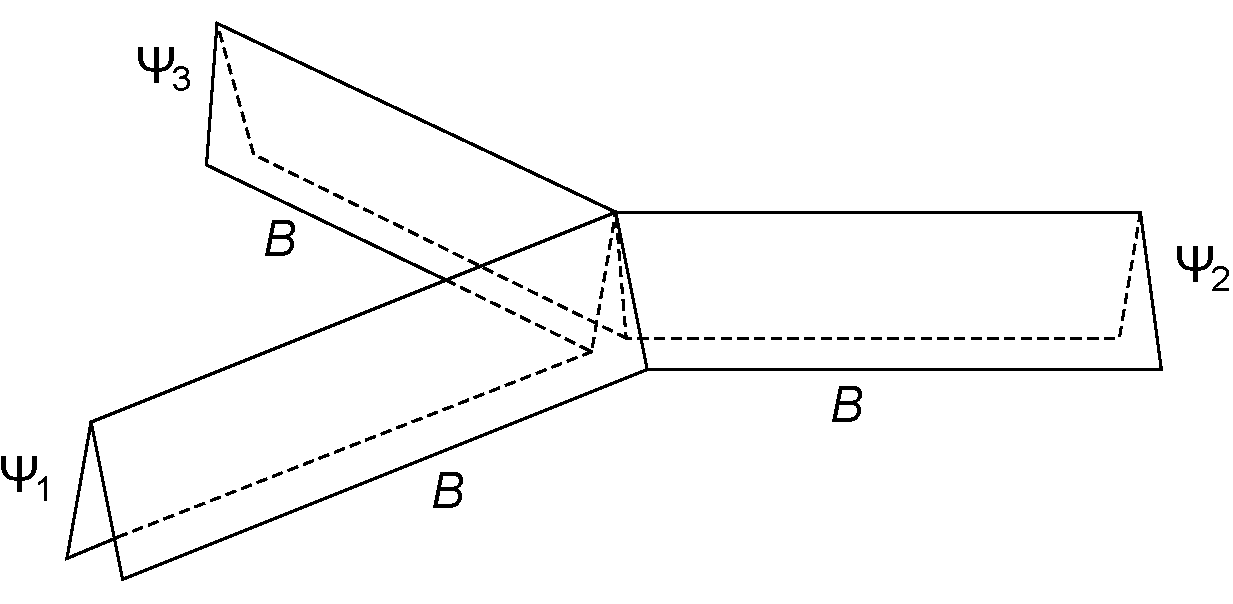
\includegraphics[width=.6\textwidth]{figures/OSFTcubicgraph.pdf}
\caption{The cubic open string vertex with three open string propagators attached. Here $B$ represents the boundary of the worldsheet, whereas the open string states $\Psi_i$ propagate along the folded strips.}\label{fig:OSFTcubicgraph}
\end{figure}

The above construction yields Witten's OSFT with only cubic vertices, whose corresponding metric geometry is visualized in Figure \ref{fig:OSFTcubicgraph}. The action (\ref{closftactbv}) reduces to simply
\ie\label{cubicbv}
S[\Psi] = {1\over 2} \langle\langle \Psi| Q_B |\Psi \rangle + {1\over 3} \{\Psi^{\otimes 3} \}_o,
\fe
The cubic vertex can be expressed in terms of boundary correlator on the UHP as\footnote{Recall that we are implicitly working with the primed open string field and disc correlator (\ref{opsftphaseredef}).}
\ie\label{fffsd}
\{\Psi_1\otimes \Psi_2\otimes \Psi_3\}_o = \left\langle \prod_{i=1}^3\left[\Psi_i(0)\right]^{(f_i)} \right\rangle_{D^2},
\fe
where the transition maps $f_i$ are defined by
\ie
f_i = h^{-1}\circ R_i\circ h.
\fe
Here 
\ie\label{hzdefz}
h(z) \equiv {1+i z \over 1-i z}
\fe
maps the $z$-UHP to the unit disc, and maps the upper half disc $\{z:{\rm Im}(z)>0, |z|<1\}$ to the right half of the unit disc. $R_i$ are the conformal transformations
\ie
R_1(w) = e^{2\pi i \over 3} w^{2\over 3},~~~~R_2(w) = w^{2\over 3}, ~~~~R_3(w) = e^{-{2\pi i \over 3}} w^{2\over 3}
\fe
that map the right half unit disc to the three wedges of the unit disc.

The star product $*$ between two open string fields is defined as the 2-string bracket associated with the cubic vertex, namely 
\ie
\Psi_1* \Psi_2 \equiv [\Psi_1\otimes \Psi_2]_o, 
\fe
or equivalently
\ie
\langle\langle \Psi_3| \Psi_1* \Psi_2 \rangle = \{ \Psi_3\otimes \Psi_1 \otimes \Psi_2 \}_o.
\fe
As all higher string brackets vanish, it follows from the $n=3$ case of (\ref{ainftyrel}) that the star product is associative. This can also be understood by viewing the star product as identifying the right half of first open string to the left half of the second open string, as is evident from Figure \ref{fig:OSFTcubicgraph}. The equation of motion reads
\ie\label{osfteq}
Q_B \Psi + \Psi*\Psi = 0,
\fe
whose solution is subject to the gauge redundancy
\ie\label{osftgaugev}
\delta_\Lambda \Psi = Q_B \Lambda - \Lambda*\Psi + \Psi*\Lambda .
\fe
A physical open string field $\Psi$ is Grassmann-odd of ghost number 1, whereas the relevant gauge transformations are generated by a Grassmann-even string field $\Lambda$ of ghost number 0.





\subsection{Open string tachyon condensation}
\label{sec:opentachyon}

We now return to the question of open string tachyon condensation on a D-brane, already hinted by the effective action (\ref{tachyoncubicop}). In the classical OSFT framework, an (a priori off-shell) open string tachyon profile that is constant on the world volume of a D-brane is represented by the open string field of the form
\ie\label{psitrial}
|\Psi\rangle = t c_1 |0\rangle + \cdots,
\fe
where $|0\rangle$ is the state that corresponds to the identity operator on the boundary of the worldsheet, $t$ is the magnitude of the tachyon field, and $\cdots$ stands for higher oscillator level states built out of $b_n$, $c_n$, and the $c^{\rm m}=26$ matter Virasoro generators $L^{\rm m}_n$.

It is instructive to evaluate the OSFT action (\ref{cubicbv}) on the simple open string field configuration $|\psi\rangle = t c_1|0\rangle$. The kinetic term evaluates to
\ie
{1\over 2} \langle\langle \psi| Q_B | \psi \rangle = {t^2\over 2}\langle 0| c_{-1} c_0 L_0 c_1 |0\rangle = -{t^2\over 2} \langle 1\rangle_{{\rm m},D^2},
\fe
whereas the cubic interaction term evaluates to
\ie\label{cuopes}
{1\over 3} \{\psi^{\otimes 3}\}_o &= {1\over 3} \prod_{i=1}^3 (\partial f_i(0))^{-1} \left\langle \psi(\sqrt{3}) \psi(0) \psi(-\sqrt{3}) \right\rangle_{D^2}
\\
& = {27\sqrt{3}\over 64} \langle 1\rangle_{{\rm m},D^2}.
\fe
The first equality in (\ref{cuopes}) follows from the conformal transformation of $\psi$ as a boundary Virasoro primary of weight $-1$.
Using $\langle 1\rangle_{{\rm m},D^2} = {V_{\rm E} \over g_o^2 \A'}$ and the relation between $g_o$ and the D-brane tension $T = {1\over 2\pi^2 g_o^2 \A'}$,\footnote{Recall that we have adopted the phase redefinition (\ref{opsftphaseredef}) and omitted the prime in notation.} we find
\ie
S[\psi] = V_{{\rm E}} T f(t),~~~~  f(t) = 2\pi^2 \left(  -{t^2\over 2} + {27\sqrt{3}\over 64}t^3 \right).
\fe
Interestingly, $f(t)$ has a local minimum at $t_* = {64\over 81\sqrt{3}}$, with $f(t_*)\approx -0.6846$. In the crude approximation where one ignores nonzero oscillator level modes of the open string field, $T f(t)$ may be viewed as the effective potential for the tachyon field $t$, and the tachyon-condensed string field configuration $|\psi\rangle = t_* c_1 |0\rangle$ acquires a negative energy density that cancels roughly $68\%$ of the D-brane tension.

One can improve the approximation by including higher oscillator level states, say up to level 2 with the ansatz
\ie
|\psi\rangle = t c_1 |0\rangle + u c_{-1}|0\rangle + v L_{-2}^{\rm m} c_1|0\rangle 
\fe
in the Siegel gauge. Now that $|\psi\rangle$ is no longer a Virasoro primary, the evaluation of the cubic interaction term is slightly more involved. The resulting action $S[\psi]$ is a cubic polynomial in $t, u, v$, which turns out to admit a stationary point where $S[\psi]$ evaluates to $\approx -0.96\cdot V_{\rm E} T$.\footnote{The relevant stationary point is no longer a local minimum of the Euclidean action, due to the presence of auxiliary fields. See Sen and Zwiebach, JHEP 03 (2000) 002 \cite{Sen:1999nx}.} That is, the approximate tachyon-condensed solution cancels $96\%$ of the D-brane tension. Higher level truncation results in the Siegel gauge strongly suggests that the exact solution of open string tachyon condensation should cancel precisely all of the D-brane tension, and describes none other than the closed string vacuum in the absence of the D-brane.

\subsubsection{Wedge states and the $\mathtt{KBc}$ algebra}
\label{sec:wedgest}

%We now introduce a number of technical ingredients that will be useful in writing down analytic solutions to Witten's cubic OSFT. 

Given a conformal map $f(z)$, we denote by $U_f$ the operator that implements the conformal transformation on ${\cal H}^o$. Explicitly, if $f(z)$ is given by exponentiating the holomorphic vector field $v(z)\partial_z$ with $v(0)=0$, namely
\ie
f(z) = e^{v(z)\partial_z} z,
\fe
then 
\ie
U_f = \exp\left[ \oint {dz\over 2\pi i} v(z) T(z) \right] = e^{ \sum_{n=0}^\infty v_n L_n },
\fe
where $v(z) \equiv \sum_{n=0}^\infty v_n z^{n+1}$, and $L_n$ are the Virasoro generators of the full worldsheet CFT of vanishing central charge. Under composition of a pair of conformal maps $f$ and $g$, we have $U_{f\circ g} = U_f U_g$.

\begin{figure}[h!]
\centering
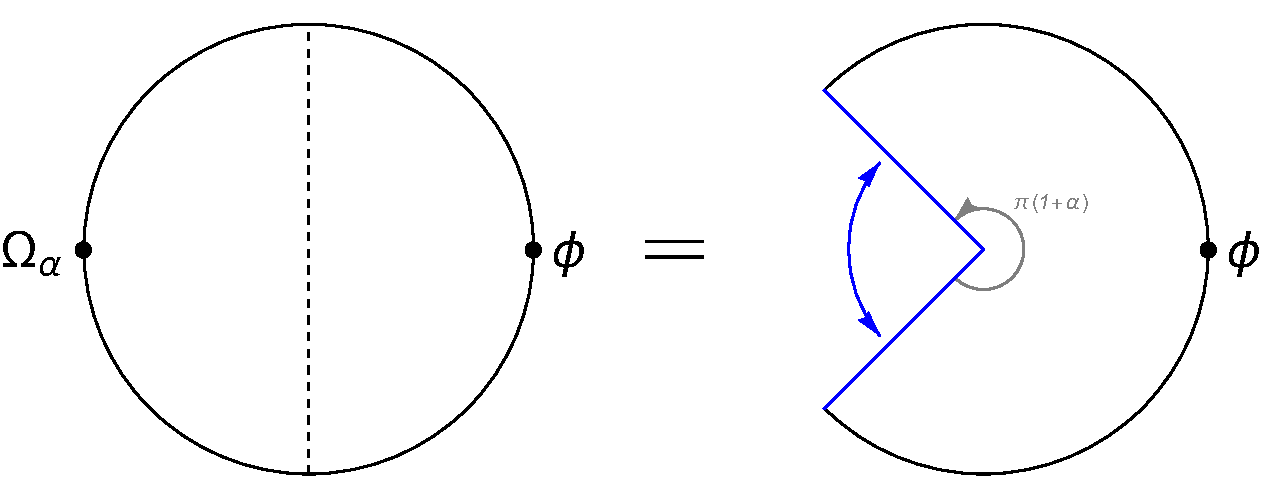
\includegraphics[width=.6\textwidth]{figures/wedgedisc.pdf}
\caption{The BPZ inner product between the wedge state $\Omega_\A$ and a general state $\phi$ (transformed into the disc coordinate via the conformal map $h$) is equivalent to the 1-point function of $\phi$ on the cone-shaped disc $\wt D^2$ with deficit angle $2\pi ( 1- {1+\A\over 2})$.}\label{fig:wedgedisc}
\end{figure}


The {\it wedge states} $|\Omega^\A\rangle$ are a family of states in the subspace of ${\cal H}^o$ spanned by the Virasoro descendants of the identity operator, that obey
\ie\label{omegaabadd}
\Omega^\A * \Omega^\B = \Omega^{\A+\B}
\fe
for any real positive $\A,\B$, with $\Omega^1 = |0\rangle$ corresponding to the boundary identity operator. Explicitly, in terms of the conformal map
\ie
f_\A = h^{-1} \circ P_\A \circ h,~~~~ P_\A(z) \equiv z^{2\over 1+\A},
\fe
with $h(z)$ defined as in (\ref{hzdefz}), the wedge state $\Omega^\A$ can be expressed as\footnote{Explicit evaluation of (\ref{omegauf}) gives $|\Omega^\A\rangle = \exp\left( {4-(1+\A)^2\over 3(1+\A)^2} L_{-2} + {(1+\A)^4-16\over 30(1+\A)^2} L_{-4} + \cdots \right) |0\rangle$. For further details see Schnabl, JHEP \textbf{01}, 004 (2003) \cite{Schnabl:2002gg}.}
\ie\label{omegauf}
\Omega^\A = U_{f_\A}^\dagger |0\rangle,
\fe
where $\dagger$ stands for the BPZ adjoint on the UHP defined via the inversion $z' = -1/z$,\footnote{Note that this differs from our convention of the BPZ adjoint on the sphere (\ref{bpzdefinv}) by a sign.} such that $L_n^\dagger = (-)^n L_{-n}$. To understand this construction, consider for any state $|\phi\rangle$, 
\ie\label{conewedgeid}
\langle\langle \Omega^\A| \phi \rangle = \langle 0| U_{f_\A} |\phi\rangle = \left\langle U_{P_\A} \cdot [\phi(0)]^h \right\rangle_{D^2} = \left\langle  [\phi(0)]^h \right\rangle_{\wt{D^2}} ,
\fe
where $\left\langle U_{P_\A} \cdot [\phi(0)]^h \right\rangle_{D^2}$ is a correlation function on the unit disc $\{w:|w|\leq 1\}$, with $U_{P_\A}$ implementing the conformal transformation $w=z^{2\over 1+\A}$. The last equality in (\ref{conewedgeid}) expresses the correlator in the $z$-coordinate, which parameterizes the cone-shaped disc $\wt{D^2}$ with a deficit angle $2\pi ( 1- {1+\A\over 2})$. The insertion of $[\phi(0)]^h$ at $z=1$ produces a state that is naturally defined on the diameter ${\rm Re}(z)=0, |z|\leq 1$. $\langle\langle \Omega^\A|$ therefore can be thought of as (the BPZ conjugate of) the state produced by the remaining wedge of $\wt{D^2}$, which spans the angle $\pi \A$, hence its namesake. With this geometric interpretation, (\ref{omegaabadd}) is evident, as the star product simply glues together a pair of wedges, produces a new wedge that spans the sum of the angles.



\begin{figure}[h!]
\centering
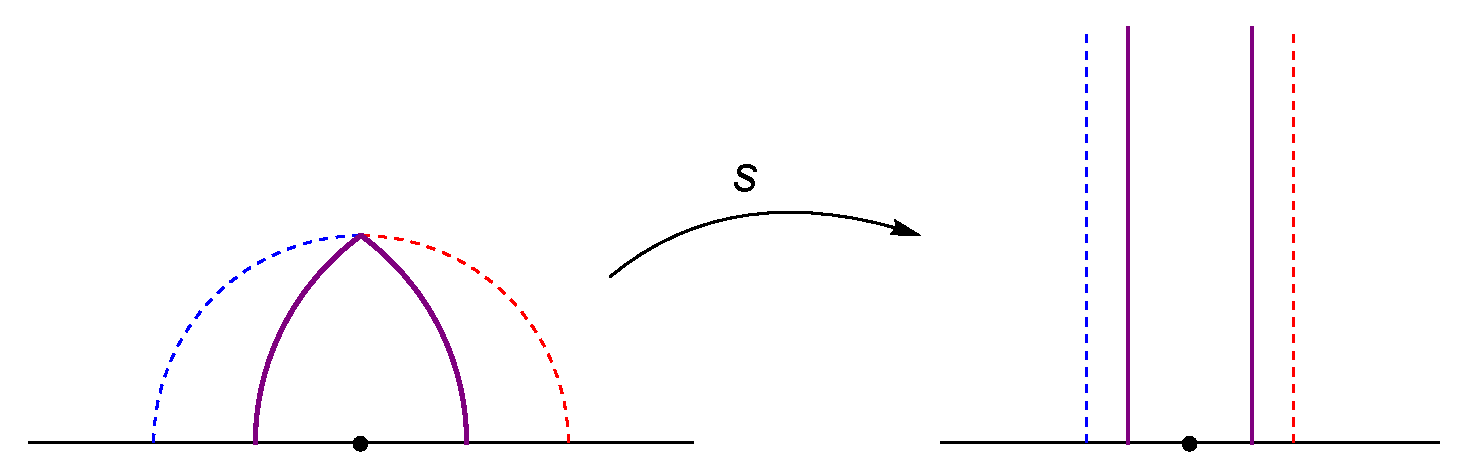
\includegraphics[width=.7\textwidth]{figures/sliver.pdf}
\caption{The sliver map $u = s(z) \equiv {2\over \pi}\arctan(z)$ takes the upper half unit $z$-disc (left) to the semi-infinite strip $|{\rm Re}(u)|\leq {1\over 2}$ on the UHP (right). The wedge bounded by purple curves on the left is mapped to the semi-infinite strip between the vertical purple lines on the right.}\label{fig:sliver}
\end{figure}


We can equivalently represent the wedge state $|\Omega^\A\rangle$ through the conformal transformation $u=s(z)$, where $s$ is the ``sliver map''
\ie\label{slivermaps}
s(z) = {1\over\pi i} \log h(z) = {2\over\pi}\arctan(z),
\fe
as the state produced by the semi-infinite vertical strip $|{\rm Re}(u)|\leq {\A\over 2}$ on the $u$-UHP. We may also write 
\ie
\Omega^\A = \exp_*(-\A \mathtt{K}),
\fe
where $\exp_*$ stands for the exponentiation defined using the $*$ product, with $\Omega^0\equiv \mathtt{I}$ playing the role of the {\it identity element} of the star algebra,\footnote{Note that $\mt{I}$ as a state is singular by itself.} i.e. $\mathtt{I}*\Psi = \Psi*\mathtt{I}=\Psi$ for any open string field $\Psi$, and
\ie
\mathtt{K} = \left.-{d\over d\A}\Omega^\A\right|_{\A=0}
\fe
may be represented as the state produced by the infinitesimally thin vertical strip on the $u$-UHP with the insertion of (in the doubling trick notation)
\ie
\int_{- i \infty}^{i\infty} {du\over 2\pi i} T(u).
\fe
We define $\mathtt{B}$ to be the state produced by the same thin strip geometry with the insertion of
\ie
\int_{- i \infty}^{i\infty} {du\over 2\pi i} b(u).
\fe
It follows that
\ie\label{kbca}
\mathtt{K} = Q_B \mathtt{B}, ~~~~ Q_B \mathtt{K} = 0,~~~~ \mathtt{B}*\mathtt{B}=0,~~~~ [\mathtt{K}, \mathtt{B}]_* = 0.
\fe
Next, we define $\mathtt{c}$ to be the state produced by the same thin strip geometry with the insertion of $c(0)$, which obeys\footnote{Note that $\mathtt{c}$ is different from $c|0\rangle$, the latter being equal to ${\pi\over 2}\, \Omega^{1\over 2}*\mathtt{c}*\Omega^{1\over 2}$.}
\ie\label{kbcb}
Q_B \mathtt{c} = \mathtt{c}* \mathtt{K} * \mathtt{c},~~~~ \mathtt{c}*\mathtt{c} = 0,~~~~ \{ \mathtt{B} , \mathtt{c} \}_* = \mathtt{I}.
\fe 
The ``$\mathtt{KBc}$ algebra'' generated by $\mathtt{K}, \mathtt{B}, \mathtt{c}$ with respect to the star product, which satisfy (\ref{kbca}), (\ref{kbcb}), will play an essential role in constructing analytic solutions of Witten's cubic OSFT.




\subsubsection{The tachyon vacuum solution}
\label{sec:tacvac}

The tachyon vacuum solution to the OSFT equation (\ref{osfteq}) can be constructed using the $\mathtt{KBc}$ algebra as\footnote{An analytic solution for the tachyon vacuum was first constructed by Schnabl, Adv. Theor. Math. Phys. \textbf{10}, no.4, 433-501 (2006) \cite{Schnabl:2005gv}. It was subsequently simplified using the $\mathtt{KBc}$ algebra by Okawa, JHEP \textbf{04}, 055 (2006) \cite{Okawa:2006vm}, and Erler, JHEP \textbf{05}, 083 (2007) \cite{Erler:2006hw}. The solution in the form (\ref{tvkbc}) was presented in Erler and Schnabl, JHEP \textbf{10}, 066 (2009) \cite{Erler:2009uj}.}
\ie\label{tvkbc}
\Psi_{\rm tv} = (\mt{c}+\mt{cKBc}) (\mt{I}+\mt{K})^{-1},
\fe
where we have adopted a notation in which all multiplication between states or string fields are understood as the $*$ product, and the inverse $(\cdots)^{-1}$ is also defined with respect to $*$, namely
\ie
(\mt{I}+\mt{K})^{-1} = \int_0^\infty d\A \, e^{-\A(\mt{I}+\mt{K})} = \int_0^\infty d\A\, e^{-\A} \Omega^\A.
\fe
In other words, (\ref{tvkbc}) is an integral of states created by the semi-infinite vertical strip of width $\A>0$ and appropriate insertions of $c, b, T$. Indeed, repeatedly using (\ref{kbca}), (\ref{kbcb}), we can evaluate
\ie
Q_B \Psi_{\rm tv} &= (\mt{cKc} + \mt{cKcKBc} - \mt{cK^2c} + \mt{cKBcKc}) (\mt{I}+\mt{K})^{-1}
\\
 &= \mt{cKc} (\mt{I}+\mt{K})^{-1}
\fe
and
\ie
\Psi_{\rm tv}^2 & =  \mt{c} (\mt{I}+\mt{K})\mt{Bc} (\mt{I}+\mt{K})^{-1}  \mt{c} (\mt{I}+\mt{K})\mt{Bc} (\mt{I}+\mt{K})^{-1}
\\
&= \mt{c}  (\mt{I}- (\mt{I}+\mt{K})\mt{c}(\mt{I}+\mt{K})^{-1}\mt{B}) \mt{c} (\mt{I}+\mt{K})\mt{Bc} (\mt{I}+\mt{K})^{-1} 
\\
&= - \mt{c}  (\mt{I}+\mt{K})\mt{c} (\mt{I}- (\mt{I}+\mt{K})^{-1} \mt{cB}(\mt{I}+\mt{K})) \mt{Bc} (\mt{I}+\mt{K})^{-1} 
\\
&= - \mt{c} \mt{K} \mt{c} (\mt{I}+\mt{K})^{-1} ,
\fe
thereby verifying that $\Psi_{\rm tv}$ obeys the equation of motion.

The physical open string fluctuations around a solution $\Psi$ are given by the cohomology of $Q_\Psi \equiv Q_B + [\Psi, \cdot\,]$. For the tachyon vacuum, we have
\ie\label{qahomtriv}
Q_{\Psi_{\rm tv}} \mt{A} = \mt{I} ~~~{\rm for}~ \mt{A} = \mt{B} (\mt{I+K})^{-1},
\fe
which implies that the cohomology of $Q_{\Psi_{\rm tv}}$ is trivial, as any $Q_{\Psi_{\rm tv}}$-closed string field $\Phi$ can be expressed as $\Phi = Q_{\Psi_{\rm tv}}(A\Phi)$. This implies that there are no physical open string excitations around the tachyon vacuum, which is consistent with the interpretation that the tachyon vacuum corresponds to the absence of the D-brane.

As the tachyon vacuum solution is homogeneous with respect to the D-brane world volume, we can determine the energy density from the OSFT action, which evaluates to
\ie
S[\Psi_{\rm tv}] &= \langle\langle \Psi_{\rm tv} | \tfrac{1}{2}  Q_B \Psi_{\rm tv}  + \tfrac{1}{3} \Psi_{\rm tv}^2 \rangle %= {1\over 6} \langle\langle \mt{I} | \Psi_{\rm tv} Q_B \Psi_{\rm tv}\rangle 
\\
&= {1\over 6} \langle\langle \mt{I} | \mt{c} (\mt{I}+\mt{K})^{-1} \mt{cKc} (\mt{I}+\mt{K})^{-1} \rangle + {1\over 6} \langle\langle \mt{I} | \mt{cKBc} (\mt{I}+\mt{K})^{-1} \mt{cKc} (\mt{I}+\mt{K})^{-1} \rangle
\fe
Using $Q_B(\mt{Bc}) = \mt{cKBc}$, the second term in the last line can be put in the form $\langle\langle I |Q_B\Phi\rangle$, which vanishes by deforming the BRST contour on the disc.\footnote{One can verify that there are no divergences that arise from the wedge states of zero width in this case.} The remaining contribution can be calculated using 
\ie\label{ckktem}
& \langle\langle \mt{I} | \mt{c} (\mt{I}+\mt{K})^{-1} \mt{cKc} (\mt{I}+\mt{K})^{-1} \rangle 
= - \int_0^\infty d\A_1 d\A_3 \,e^{-\A_1-\A_3} \partial_{\A_2}|_{\A_2=0}\langle\langle\mt{I}| \mt{c} \Omega^{\A_1} \mt{c} \Omega^{\A_2} \mt{c} \Omega^{\A_3} \rangle,
\fe
where $\langle\langle\mt{I}| \mt{c} \Omega^{\A_1} \mt{c} \Omega^{\A_2} \mt{c} \Omega^{\A_3} \rangle$ is none other than the correlation function on the semi-infinite cylinder of circumference $\A_1+\A_2+\A_3$ and insertions of three $c$ ghosts on the boundary, separated by distance $\A_1$, $\A_2$, $\A_3$, giving
\ie
\langle\langle\mt{I}| \mt{c} \Omega^{\A_1} \mt{c} \Omega^{\A_2} \mt{c} \Omega^{\A_3} \rangle
= \langle 1 \rangle_{{\rm m},D^2} \left( {\A_1+\A_2+\A_3\over \pi} \right)^3 \prod_{i=1}^3 \sin{\pi \A_i\over \A_1+\A_2+\A_3} .
\fe
Evaluating the integral in (\ref{ckktem}) then yields
\ie
S[\Psi_{\rm tv}] = - {1\over 2\pi^2} \langle 1 \rangle_{{\rm m},D^2} = - V_{\rm E} T,
\fe
precisely canceling the tension of the D-brane, as anticipated.



\subsection{More general solutions of the bosonic OSFT}

\subsubsection{Marginal deformations}
\label{sec:margok}

A marginal deformation of the boundary conformal field theory (BCFT) is generated by a weight 1 boundary primary $V$, and amounts to inserting $\exp\left( \lambda \int_{\partial\Sigma} V \right)$ into the correlation functions of the CFT on the surface $\Sigma$. The precise definition of the exponential of the integrated operators requires the choice of a regularization scheme (e.g. point-splitting), which a priori may violate conformal invariance beyond the first order in $\lambda$. We say that the deformation is {\it exactly} marginal if conformal invariance is preserved to all orders in $\lambda$.\footnote{A priori, one may worry that the perturbative expansion of observables with respect to $\lambda$ may not converge. Nonetheless, a generic (B)CFT is expected to reside at a regular point on the conformal manifold of exactly marginal deformations, near which the conformal spectral data are expected to depend analytically on the coordinates of the conformal manifold that include $\lambda$. Counterexamples to this expectation typically occur in a noncompact CFT that arise as an accumulation point of a discrete family of compact CFTs.}



An exactly marginal deformation of the matter BCFT on the string worldsheet may also be viewed as a deformation of the corresponding D-brane configuration. The background independence of OSFT suggests that such a deformation can be equivalently represented by a solution to the open string field equation (\ref{osfteq}), which admits a perturbative expansion of the form
\ie\label{pertosftsoex}
\Psi = \sum_{n=1}^\infty \lambda^n \Psi^{(n)}.
\fe
The first order solution is simply
\ie
\Psi^{(1)} = c V,
\fe
where $V$ is a weight 1 matter BCFT primary, and satisfies $Q_B \Psi^{(1)} = 0$. It will be useful to represent the BPZ inner product $\Psi^{(1)}$ with an arbitrary state $\phi$ in the form
\ie
\langle\langle\phi| \Psi^{(1)}\rangle = \left\langle \left[ \phi(0)\right]^s c V(1) \right\rangle_{{\cal W}_1},
\fe
where $s$ is the sliver map (\ref{slivermaps}), and ${\cal W}_n$ stands for the semi-infinite cylinder obtained by identifying $z\sim z+n+1$ on the UHP.

We now present an all-order solution due to Kiermaier and Okawa, JHEP \textbf{11} (2009), 041 \cite{Kiermaier:2007vu}. Let us first make a simplifying assumption that the operator product $V(y_1)\cdots V(y_n)$ is integrable with respect to $y_i$ in the limit where the $y_i$'s coincide with one another. In this case, the second order equation $Q_B \Psi^{(2)} = - \Psi^{(1)}*\Psi^{(1)}$ can be solved with a string field $\Psi_L^{(2)}$ that obeys
\ie\label{koksecsol}
\langle\langle\phi| \Psi_L^{(2)}\rangle = \left\langle \left[ \phi(0)\right]^s c V(1) V(1,2) \right\rangle_{{\cal W}_2},
\fe
where $V(a, b) \equiv \int_a^b dy V(y)$. Indeed, we can verify
\ie\label{qbcseondorderv}
\langle\langle\phi| Q_B \Psi_L^{(2)}\rangle &= - \left\langle \left[ \phi(0)\right]^s c V(1) Q_B V(1,2) \right\rangle_{{\cal W}_2}
\\
&=  - \left\langle \left[ \phi(0)\right]^s c V(1) \int_1^2 dy \partial_y c V(y) \right\rangle_{{\cal W}_2}
\\
&=  - \left\langle \left[ \phi(0)\right]^s c V(1) c V(2) \right\rangle_{{\cal W}_2} =  - \langle\langle\phi| \Psi^{(1)} * \Psi^{(1)} \rangle.
\fe
%where in arriving at the third equality we have used the property that the $V(1) V(y)$ OPE contains no term of order $(y-1)^{-1}$ in the $y\to 1$ limit (as such a term would lead to a nontrivial beta function that obstructs exactly marginality at the second order), and have subtracted any possible power divergences near $y=1$. Similarly, the RHS of (\ref{koksecsol}) should also be understood as defined by subtracting off possible power divergences due to the $VV$ OPE. 
This construction can be extended to an all-order {\it complex} string field $\Psi_L = \sum_{n=1}^\infty \lambda^n \Psi_L^{(n)}$ that obeys $Q_B \Psi_L + \Psi_L * \Psi_L=0$, where $\Psi_L^{(n)}$ is given by
\ie\label{psilallord}
\langle\langle\phi| \Psi_L^{(n)}\rangle = \left\langle \left[ \phi(0)\right]^s c V(1) \int_1^2 dy_1 V(y_1) \int_{y_1}^3 dy_2 V(y_2) \cdots \int_{y_{n-2}}^{n} dy_{n-1} V(y_{n-1}) \right\rangle_{{\cal W}_n}.
\fe 
However, due to the left-right asymmetry of the $V$ insertions on the RHS of (\ref{psilallord}), $\Psi_L$ does not obey the reality condition on the open string field. One can construct another complex string field solution $\Psi_R = \sum_{n=1}^\infty \lambda^n \Psi_R^{(n)}$, where $\Psi_R^{(n)}$ is given by (\ref{psilallord}) with the $V$ insertions reversed in order, namely
\ie\label{psilallordr}
\langle\langle\phi| \Psi_R^{(n)}\rangle = \left\langle \left[ \phi(0)\right]^s \int_{n-1}^n dy_{n-1}' \int_{n-2}^{y_{n-1}'} dy_{n-2}' \cdots \int_1^{y'_2} dy'_1 V(y'_1) \cdots V(y'_{n-1}) cV(n) \right\rangle_{{\cal W}_n}.
\fe
In fact, $\Psi_R$ and $\Psi_L$ are related by a complexified gauge transformation
\ie
\Psi_R = U^{-1}* \Psi_L * U + U^{-1}* Q_B U ,
\fe
where
\ie\label{uunregdef}
U = 1+ \sum_{n=1}^\infty \lambda^n U^{(n)},~~~~\langle\langle\phi| U^{(n)}\rangle = {1\over n!} \left\langle \left[ \phi(0)\right]^s (V(1,n))^n \right\rangle_{{\cal W}_n},
\fe
and $U^{-1}$ is the $*$-inverse of $U$. A real open string field solution $\Psi$ that represents the desired exactly marginal deformation can then be constructed as
\ie\label{psirealrecov}
\Psi = U^{-{1\over 2}}* \Psi_L * U^{1\over 2} + U^{-{1\over 2}}* Q_B U^{1\over 2} ,
\fe
where $U^{\pm{1\over 2}}$ are defined by the properties $U^{-{1\over 2}}* U^{1\over 2} = 1$ and $U^{1\over 2}* U^{1\over 2} = U$.

More generally, when the OPE $V(y_1)\cdots V(y_n)$ is not integrable in the coincidence limit, the exactly marginal deformation of the matter BCFT may be defined via the insertion of $\left[ e^{\lambda \int dy V(y)} \right]_r$, where $[\cdots ]_r$ stands for a suitably regularized operator product. In particular, the insertion of
\ie\label{deforintval}
\left[ e^{\lambda V(y_L,y_R)} \right]_r = \sum_{n=0}^\infty {\lambda^n\over n!} \left[ (V(y_L,y_R))^n \right]_r
\fe
into a correlation function on the UHP amounts to modifying the boundary condition in the interval $(y_L,y_R)$ to the deformed matter BCFT (which we will denote by BCFT$_\lambda$). Equivalently, (\ref{deforintval}) may be represented as the product of a pair of interface operators $W_L(y_L) W_R(y_R)$, where $W_L \in {\cal H}_{0\lambda}$, $W_R\in {\cal H}_{\lambda 0}$, ${\cal H}_{\lambda\lambda'}$ being the space of boundary operators interpolating between BCFT$_\lambda$ and BCFT$_{\lambda'}$. Note that the operators $W_L, W_R$ generally depend on the choice of regularization scheme.

Applying the BRST operator to (\ref{deforintval}) now yields
\ie\label{qblambvvreg}
Q_B \left[ e^{\lambda V(y_L,y_R)} \right]_r &=  W_L(y_L) (Q_B W_R(y_R)) + (Q_B W_L(y_L)) W_R(y_R)
\\
&= \left[ e^{\lambda V(y_L,y_R)} O_R(y_R) \right]_r - \left[ O_L(y_L) e^{\lambda V(y_L,y_R)} \right]_r,
\fe
for some suitable boundary operator $O_{L/R} = \sum_{n=1}^\infty \lambda^n O_{L/R}^{(n)}$ in the original matter BCFT. We have already seen in the derivation of (\ref{qbcseondorderv}) that $O_R^{(1)} = O_L^{(1)} = c V$. If the only marginal or relevant term in the OPE of a pair of $V$'s is the identity operator, namely $V(y) V(0) = y^{-2} + o(y^{-1})$, then one finds $O_R^{(2)} = - O_L^{(2)} = {1\over 2} \partial c$.

For $U$ defined by the regularized version of (\ref{uunregdef}), namely
\ie
U = 1+ \sum_{n=1}^\infty \lambda^n U^{(n)},~~~~\langle\langle\phi| U^{(n)}\rangle = {1\over n!} \left\langle \left[ \phi(0)\right]^s \left[ (V(1,n))^n\right]_r \right\rangle_{{\cal W}_n},
\fe
it follows from (\ref{qblambvvreg}) that
\ie{}
Q_B U = A_R - A_L,
\fe
where $A_L$ and $A_R$ are defined by
\ie{}
& \langle\langle\phi| A_L^{(n)}\rangle = \sum_{\ell=1}^n {1\over (n-\ell)!} \left\langle \left[ \phi(0)\right]^s \left[ O_L^{(\ell)} (V(1,n))^{n-\ell}\right]_r \right\rangle_{{\cal W}_n},
\\
& \langle\langle\phi| A_R^{(n)}\rangle = \sum_{\ell=1}^n {1\over (n-\ell)!} \left\langle \left[ \phi(0)\right]^s \left[ (V(1,n))^{n-\ell}O_R^{(\ell)} \right]_r   \right\rangle_{{\cal W}_n}.
\fe
Next, one constructs the complex string fields
\ie
\Psi_L = A_L * U^{-1},~~~~ \Psi_R = U^{-1} * A_R,
\fe
which can be shown to agree with (\ref{psilallord}), (\ref{psilallordr}) in the case where the OPEs of $V$'s are integrable (and $O_L = O_R = cV$ to all orders in $\lambda$). More generally, one can verify that 
\ie
Q_B A_R = - Q_B A_L = A_L*U^{-1}*A_R,
\fe
from which it follows easily that $Q_B\Psi_{L/R} + \Psi_{L/R}*\Psi_{L/R}=0$. A real open string field solution $\Psi$ is then recovered as in (\ref{psirealrecov}).

A particularly interesting example is that of the Neumann boundary condition of a single free boson $X$, deformed by the insertion of
\ie\label{vmargcosx}
\left[ e^{\lambda\int_{\partial\Sigma} V} \right]_r,~~~~ V = \sqrt{2} \cos {X\over \sqrt{\A'}} .
\fe
To begin with, $V$ is a weight 1 boundary primary that obeys the OPE $V(y) V(0) = y^{-2} - {1\over 2\A'} (\partial X)^2(0) + {\cal O}(y)$. The structure of the more general OPE $V(y_1)\cdots V(y_n)$ can be understood through the following trick. Had we compactified $X$ at the self-dual radius, namely $X\sim X + 2\pi \sqrt{\A'}$, the bulk CFT is equivalent to the $SU(2)$ WZW model at level 1,\footnote{See e.g. section 8.3 of Polchinski, {\it String theory. Vol. 1} \cite{Polchinski:1998rq}.} and the three boundary operators $\left(\sqrt{2} \cos {X\over \sqrt{\A'}}, \sqrt{2} \sin {X\over \sqrt{\A'}}, {i\over \sqrt{2\A'}} \partial X\right)$ are related by a diagonal subgroup of the global $SU(2)\times SU(2)$ symmetry. Therefore, the singularity structure of $V(y_1)\cdots V(y_n)$ is identical to that of the free field product $V'(y_1)\cdots V'(y_n)$ where $V' \equiv {i\over \sqrt{2\A'}} \partial X$, computed via Wick contractions. This property continues to hold for any compactification radii that are integer multiples of $\sqrt{\A'}$, as well as for the noncompact free boson, despite the absence of the $SU(2)$ symmetry away from the self-dual radius. As such, we can define the regularization $[\cdots ]_r$ in (\ref{vmargcosx}) simply by subtracting off the power divergences due to the Wick contractions in the coincidence limit,\footnote{Note that this regularization scheme is not equivalent to the boundary normal ordering $\vdots \, \vdots$, as $\vdots V(y_1) V(y_1, y_2) \vdots =  \left[ V(y_1) V(y_1, y_2) \right]_r + {1\over y_2-y_1}$.} e.g.
\ie
\left[ V(y_1) V(y_1, y_2) \right]_r = \lim_{\epsilon\to 0} \left[\int_{y_1+\epsilon}^{y_2} dy V(y_1) V(y) - {1\over \epsilon} \right].
\fe
The $SU(2)$ trick can be further used to show that the deformation (\ref{vmargcosx}) is exactly marginal. The boundary state $|B_\lambda\rangle$ of the deformed BCFT can be explicitly constructed as follows. Starting with the compact boson at self-dual radius and the Neumann boundary state $|N \rangle_{R=\sqrt{\A'}}$, we can write the deformed boundary state as
\ie\label{bsutworota}
|B_\lambda\rangle_{R=\sqrt{\A'}} = \exp \left(  \sqrt{2} \lambda \oint dz\, j^1(z) \right) |N\rangle_{R=\sqrt{\A'}},
\fe
where $j^1(z) = \cos( {2\over \sqrt{\A'}} X_L(z))$ is one of the holomorphic $SU(2)_1$ currents, and the contour integral in the exponent is understood as a conserved charge operator. The boundary limit of $j^1$ is $\cos{X\over \sqrt{\A'}}$, and the successive holomorphic contour integrals in the series expansion of the exponential effectively implements the subtraction of power divergences, thereby producing a deformation equivalent to (\ref{vmargcosx}). In fact, the exponential operator on the RHS of (\ref{bsutworota}) is none other than a holomorphic $SU(2)$ rotation (around the $j^1$-axis) by the angle $\pi \sqrt{2} \lambda$. Moreover, one can show that in the special case $\lambda = {1\over 2\sqrt{2}}$, corresponding to rotation angle ${\pi\over 2}$, the deformed BCFT is that of a Dirichlet boundary condition.\footnote{Callan et al., Nucl. Phys. B \textbf{422} (1994), 417 \cite{Callan:1994ub}; Recknagel and Schomerus, Nucl. Phys. B \textbf{545} (1999), 233 \cite{Recknagel:1998ih}.} The analogous boundary state $|B_\lambda\rangle_{R=\infty}$ in the noncompact free boson CFT can be obtained from $|B_\lambda\rangle_{R=\sqrt{\A'}}$ by projecting out the winding modes. As $\lambda$ ranges from 0 to ${1\over 2\sqrt{2}}$, the deformed BCFT interpolates between that of the Neumann boundary condition and that of an infinite array of codimension-1 D-branes located at $X = (2n+1)\pi \sqrt{\A'}$, $n \in \mathbb{Z}$.

In the OSFT description, the deformation (\ref{vmargcosx}) is described by the Kiermaier-Okawa solution, where (\ref{vmargcosx}) is satisfied exactly for
\ie
{\cal O}_L = \lambda c V - {\lambda^2\over 2} \partial c,~~~~ {\cal O}_R = \lambda c V + {\lambda^2\over 2} \partial c.
\fe
%where the order $\lambda^{n\geq 3}$ terms are absent.

\subsubsection{Rolling tachyon revisited}
\label{sec:rollingosft}

The rolling tachyon on the ZZ-brane of $c=1$ string theory was described from the worldsheet perspective in section \ref{sec:zzrolling} as the BCFT deformation (\ref{deformarolltac}), which may be viewed as the Wick rotation of (\ref{vmargcosx}) defined by the replacement $X\to i X^0$ in the free boson sector, together with the decoupled ZZ-boundary condition in the Liouville sector. From the perspective of on-shell string perturbation theory, it is not immediately obvious how to define physical observables analogous to the scattering amplitudes of asymptotic states due to the explicit time-dependence in the spacetime background.\footnote{It is conceivable that a suitable notion of S-matrix in the time-dependent background can be defined with a choice of in- and out-vacuum states that corresponds to a choice of the contour in the field space of the worldsheet path integral.} Some clues can be found by inspecting the deformed matter boundary state $|B\rangle = |B\rangle_{X^0}\otimes |B_{\rm ZZ}\rangle$, where
\ie\label{bdryfg}
|B\rangle_{X^0} \propto f(X^0) |0\rangle + g(X^0) \A_{-1} \wt\A_{-1} |0\rangle + \cdots .
\fe
Here $\cdots$ stands for higher oscillator level states, and the functions $f(X^0), g(X^0)$ are given by
\ie\label{bdryfgexp}
& f(X^0) = {1\over 1+ e^{X^0\over \sqrt{\A'}} \sin(\pi\wt\lambda) } + {1\over 1+ e^{-X^0\over \sqrt{\A'}} \sin(\pi\wt\lambda) }  - 1,  
\\
& g(X^0) = 1 + \cos(2\pi\wt\lambda) - f (X^0).
\fe
Heuristically, one expects $f(X^0)$ and $g(X^0)$ to represent sources for the dilaton and graviton fields. Indeed, the quantity $f(X^0) + g(X^0)$ which is conserved in time was interpreted, up to a normalization factor, as the energy of the rolling tachyon by Sen, JHEP \textbf{04}, 048 (2002) \cite{Sen:2002nu}, which is further justified by considering coupling to closed string fields in Sen, JHEP \textbf{12} (2004), 053 \cite{Sen:2004yv}.

In the OSFT description, the rolling tachyon is described by a solution $\Psi$ to the equation of motion of the perturbative form (\ref{pertosftsoex}), whose first order term is given by $\Psi^{(1)} = c \cosh({X^0\over \sqrt{\A'}})$, and the all-order solution can be constructed by the method of section \ref{sec:margok}. In this approach, the underlying BCFT is undeformed, and the time-dependence is characterized explicitly through the string field solution. 

It is somewhat nontrivial to identify the energy of the open string field, however, as the classical OSFT is formulated through a Lagrangian that contains a priori arbitrarily high order time derivatives, to which one cannot simply apply the canonical formalism. Nonetheless, the Hamiltonian of the OSFT can be constructed indirectly through the covariant phase space formalism.\footnote{Witten, Nucl. Phys. B \textbf{276} (1986), 291 \cite{Witten:1986qs}. See also Lee and Wald, J. Math. Phys. \textbf{31} (1990), 725 \cite{Lee:1990nz}, and Harlow and Wu, JHEP \textbf{10} (2020), 146 \cite{Harlow:2019yfa}.} The basic idea is that given an action $S = \int_M {\cal L}$ where $M$ is the spacetime and ${\cal L}$ the Lagrangian density, the classical {\it pre-phase space} $\wt{\mathfrak P}$ is the space of solutions to the equation of motion $e_a=0$ obtained by varying the Lagrangian with respect to the fields $\phi^a$,
\ie
\delta L = e_a \delta\phi^a + d U.
\fe
$U$ is known as the pre-symplectic potential, which can be viewed as a 1-form on $\wt{\mathfrak P}$. The pre-symplectic form $\wt\Omega$ is a differential 2-form on $\wt{\mathfrak P}$ defined as
\ie
\wt \Omega = \int_{\Sigma} \delta U,
\fe
where $\Sigma$ is a Cauchy slice, essentially a constant-time slice of $M$, and $\delta$ which stands for an infinitesimal variation of the field is now viewed as an exterior derivative on $\wt{\mathfrak P}$. In a gauge theory, the phase space $\mathfrak{P}$ is obtained as the quotient of $\wt{\mathfrak P}$ by the group of gauge transformations, and is equipped with a symplectic form $\Omega$ that is inherited from $\wt\Omega$. In particular, the time translation of the solution can be viewed as a vector field ${\delta/ \delta t}$ on ${\mathfrak P}$, and is related to the Hamiltonian $H$ through
\ie
\delta H = \iota_{\delta/ \delta t} \Omega,
\fe
where $\iota_v$ stands for the interior product of a form with the vector field $v$.

Applying this procedure to the OSFT, we begin by writing the variation of the action (\ref{cubicbv}) as
\ie
\delta S = \int (Q_B \Psi + \Psi*\Psi)* \delta\Psi - {1\over 2} Q_B (\Psi* \delta\Psi),
\fe
where the convolution $\int$ is defined as
\ie
\int \Psi = \langle\langle \mathtt{I} | \Psi\rangle.
\fe
Here $\mathtt{I} = \Omega^0$ is the identity element of the star algebra represented by the zero width wedge state, as seen in section \ref{sec:wedgest}. A candidate pre-symplectic potential, proposed by Witten, is
\ie
U = - {1\over 2} \int [Q_B, \Theta(\Sigma)] (\Psi*\delta\Psi),
\fe
where $\Theta(\Sigma)$ is the Heaviside step function with respect to the open string midpoint. That is, $\Theta(\Sigma)$ is defined to be 1 if the open string midpoint is to the future of the Cauchy slice $\Sigma$, and 0 otherwise. As $Q_B$ involves up to 2 derivatives with respect to $X^0$, the commutator with $\Theta(\Sigma)$ serves to strip off one time derivative. This results in a symplectic form that is formally gauge invariant and independent of the choice of the slice $\Sigma$. However, its definition via the star product implicitly involves a conformal transformation that acts singularly on the operator $[Q_B, \Theta(\Sigma)]$, rendering the result potentially ill-defined. A simple fix turns out to be replacing $[Q_B, \Theta(\Sigma)]$, understood as a local operator inserted at the midpoint of the string, with its zero weight component
\ie\label{dthetadef}
D \equiv \mathbb{P} [Q_B, \Theta(\Sigma)],
\fe
where $\mathbb{P}$ is the projector onto the weight $(0,0)$ subspace. This leads to the symplectic form\footnote{Cho, Mazel and Yin, JHEP \textbf{04} (2025), 129 \cite{Cho:2023khj}.}
\ie\label{omegasympwitfix}
\Omega &= - {1\over 2} \int D (\delta\Psi*\delta\Psi)
\\
&= - {1\over 2} \left\langle D(i) \left[ \delta\Psi(0) \right]^{h_1} \left[ \delta\Psi(0) \right]^{h_2} \right\rangle_{\rm UHP},
\fe
where $h_1, h_2$ are the conformal maps $h_1(w) = {1+w\over 1-w}$ and $h_2(w) = - {1-w\over 1+w}$. Using the fact that the projector $\mathbb{P}$ commutes with $Q_B$ and the cyclicity of the convolution, one can verify that $\Omega$ is gauge-invariant, vanishes on a gauge-trivial string field variation, and is independent of the choice of the slice $\Sigma$ up to possible spatial boundary terms.

Explicitly, we may take $\Sigma$ to be the constant time slice $X^0 = t_0$, and represent $\Theta(\Sigma)$ as
\ie
\Theta(\Sigma_{X^0 = t_0}) = \int_{-\infty}^\infty {d\omega\over 2\pi i} {e^{i\omega (X^0 - t_0)} \over \omega - i \epsilon}.
\fe
A straightforward computation of (\ref{dthetadef}) gives
\ie
D &=  \mathbb{P} \int_{-\infty}^\infty {d\omega\over 2\pi} {e^{i\omega (X^0 - t_0)} } \left[ c \partial X^0 + \wt c \bar\partial X^0 + \cdots \right]
\\
&= {1\over V_{X^0}} \left( c \partial X^0 + \wt c \bar\partial X^0 \right),
\fe
where $V_{X^0}$ is the volume in time.

It is instructive to demonstrate (\ref{omegasympwitfix}) using the first order rolling tachyon solution, $\Psi = \lambda c \cosh({X^0-u\over \sqrt{\A'}} ) + {\cal O}(\lambda^2)$, where the parameters $(\lambda, u)$ can be viewed as phase space coordinates. Substituting the variation
\ie
\delta\Psi = \delta \lambda c \cosh(\tfrac{X^0-u}{ \sqrt{\A'}} ) - \tfrac{1}{ \sqrt{\A'}} \delta u \lambda c \sinh(\tfrac{X^0-u}{ \sqrt{\A'}}  ) + {\cal O}(\lambda^2)
\fe
into (\ref{omegasympwitfix}), we find the symplectic form
\ie\label{omegafirstord}
\Omega &= - {\lambda \delta u \wedge \delta \lambda\over 2 \sqrt{\A'}} \Big\langle D(i) \big[ c \sinh(\tfrac{X^0-u}{ \sqrt{\A'}} )(1) \,c \cosh(\tfrac{X^0-u}{ \sqrt{\A'}} )(-1)
\\
&~~~~~~~~~~~~~~~~~~~~~~~~~~ - c \cosh(\tfrac{X^0-u}{ \sqrt{\A'}} )(1)\, c \sinh(\tfrac{X^0-u}{ \sqrt{\A'}} )(-1)  \big] \Big\rangle_{\rm UHP} + {\rm higher~order}
\\
& = - {\lambda \over g_o^2 \A'} \delta u \wedge \delta \lambda + {\rm higher~order} .
\fe
The energy of the rolling tachyon $E(\lambda)$ is related by
\ie
\Omega = \delta u \wedge \delta E(\lambda).
\fe
From (\ref{omegafirstord}), we can read off
\ie
E(\lambda) = {1\over 2\pi^2 g_o^2\A'} \left[ 1 - \pi^2 \lambda^2 + {\cal O}(\lambda^3) \right],
\fe
where the order $\lambda^0$ term is the mass of the ZZ-brane itself. This result is precisely in agreement with (\ref{elamrolttare}). In fact, it can be shown to all orders \cite{Cho:2023khj} that the $\lambda$-dependence of $E(\lambda)$ is proportional to that of the so-called Ellwood invariant
\ie
W(\Psi, D) \equiv \langle\langle\Omega^0 | D(i) |\Psi\rangle = \left\langle D(i) [\Psi(0)]^f \right\rangle_{\rm UHP},
\fe
where $f(w) = {2w\over 1-w^2}$ is the conformal map that takes the half unit disc to the UHP. An essential property of $W(\Psi, D)$ is that it admits an equivalent expression in terms of the deformed boundary state $|B_{\wt\lambda}\rangle$,\footnote{Ellwood, JHEP \textbf{08} (2008), 063 \cite{Ellwood:2008jh}.}
\ie
W(\Psi, D) = {i\over 2\pi} \left[ \langle B_{\wt\lambda}| c_0^-| D\rangle - \langle B_{0}| c_0^-| D\rangle \right],
\fe
which through (\ref{bdryfg}), (\ref{bdryfgexp}) then establishes the exact expression of the energy of the rolling tachyon, $E = {1\over 4\pi^2 g_o^2 \A'} \left(1+\cos(2\pi\wt\lambda)\right)$.





\subsubsection{The Erler-Maccaferri solutions}

Given a pair of matter boundary conformal field theories BCFT$_0$ and BCFT$_*$ corresponding to two different D-brane configurations, not necessarily related by marginal deformations, the expectation of background independence is such that the OSFT based on BCFT$_0$ should admit a nontrivial solution that is physically equivalent to changing the D-brane configuration into that of BCFT$_*$. A remarkable construction for such an open string field solution was found by Erler and Maccaferri, JHEP \textbf{01} (2020), 021 \cite{Erler:2019fye}, which we now describe. 

Let ${\cal H}_0$ and ${\cal H}_*$ be the space of open string fields based on BCFT$_0$ and BCFT$_*$ respectively. We will write $\Psi_{{\rm tv},0}$ and $\Psi_{{\rm tv},*}$ for the tachyon vacuum solution, given by (\ref{tvkbc}) up to a gauge transformation, in the two OSFTs respectively. Let ${\cal H}_{0*}$, ${\cal H}_{*0}$ be the space of open string fields interpolating between the two boundary conditions. The idea of Erler and Maccaferri is to construct a solution of the OSFT based on BCFT$_0$ of the form
\ie\label{psiintertw}
\Psi_* = \Psi_{{\rm tv},0} - \Sigma \Psi_{{\rm tv},*} \overline\Sigma.
\fe
Here and below all products between string fields, unless otherwise noted, are understood as $*$-product. $\Sigma\in {\cal H}_{0*}$ and $\overline\Sigma \in {\cal H}_{*0}$ are {\it intertwining fields} that obey
\ie\label{qsigmapsi}
& Q_{\Psi_{\rm tv}} \Sigma\equiv Q_B \Sigma + \Psi_{{\rm tv},0}\Sigma - \Sigma\Psi_{{\rm tv},*} = 0,
\\
& Q_{\Psi_{\rm tv}} \overline\Sigma\equiv Q_B \overline\Sigma + \Psi_{{\rm tv},*}\overline\Sigma - \overline\Sigma\Psi_{{\rm tv},0} = 0,
\fe
and
\ie\label{sigmasigmaone}
\overline\Sigma \Sigma = \mathtt{I}.
\fe
For convenience of notation we will drop the subscript $0, *$ on $\Psi_{\rm tv}$. Given the properties (\ref{qsigmapsi}), (\ref{sigmasigmaone}), it is easy to verify that (\ref{psiintertw}) solves the equation of motion:
\ie
Q_B\Psi_* &= Q_B \Psi_{\rm tv} - (Q_B \Sigma) \Psi_{\rm tv} \overline\Sigma - \Sigma (Q_B \Psi_{\rm tv}) \overline\Sigma  + \Sigma \Psi_{\rm tv} Q_B \overline\Sigma
\\
&= - \Psi_{\rm tv}^2 + \Psi_{\rm tv} \Sigma  \Psi_{\rm tv} \overline\Sigma - \Sigma \Psi_{\rm tv}^2 \overline\Sigma + \Sigma \Psi_{\rm tv}^2 \overline\Sigma - \Sigma \Psi_{\rm tv}^2 \overline\Sigma + \Sigma \Psi_{\rm tv} \overline\Sigma \Psi_{\rm tv}
\\
&= - \Psi_{{\rm tv}}^2 + \Psi_{\rm tv} \Sigma \Psi_{{\rm tv}} \overline\Sigma - \Sigma \Psi_{{\rm tv}} \overline\Sigma \Sigma \Psi_{{\rm tv}} \overline\Sigma + \Sigma \Psi_{{\rm tv}} \overline\Sigma \Psi_{\rm tv} = - \Psi_*^2.
\fe
It will be useful to consider the {\it homotopy operators} $\mathtt{A}_0\in {\cal H}_0$ and $\mathtt{A}_*\in {\cal H}_*$ that satisfy
\ie\label{eqahomot}
Q_{\Psi_{\rm tv}}\mathtt{A} = \mathtt{I},~~~~\mathtt{A}^2=0,
\fe
where $\mathtt{I}=\Omega^0$ is the identity string field, in the two OSFTs respectively. The first equation of (\ref{eqahomot}) reflects that the cohomology of $Q_{\Psi_{\rm tv}}$ is trivial, as already seen in (\ref{qahomtriv}). The second equation of (\ref{eqahomot}) is an extra condition that is also satisfied by (\ref{qahomtriv}), and will be used in (\ref{sigmamasgder}) below. The intertwining fields can be constructed as
\ie
\Sigma = Q_{\Psi_{\rm tv}} (\mathtt{A} \Sigma_{\rm pre}),~~~~ \overline \Sigma = Q_{\Psi_{\rm tv}} (\overline \Sigma_{\rm pre} \mathtt{A}),
\fe
where $\Sigma_{\rm pre}\in {\cal H}_{0*}$ and $\overline\Sigma_{\rm pre} \in {\cal H}_{*0}$ satisfy
\ie\label{sigmapreaa}
\overline\Sigma_{\rm pre} \mathtt{A} \Sigma_{\rm pre} = \mathtt{A},
\fe
Obviously (\ref{qsigmapsi}) is satisfied. It follows from (\ref{eqahomot}) and (\ref{sigmapreaa}) that 
\ie\label{sigmamasgder}
\overline\Sigma \mathtt{A} \Sigma &= Q_{\Psi_{\rm tv}} (\overline \Sigma_{\rm pre} \mathtt{A}) \mathtt{A} Q_{\Psi_{\rm tv}} (\mathtt{A} \Sigma_{\rm pre})
\\
&= \overline \Sigma_{\rm pre} \mathtt{A} (Q_{\Psi_{\rm tv}} \mathtt{A}) ((Q_{\Psi_{\rm tv}} \mathtt{A}) \Sigma_{\rm pre} -  \mathtt{A} Q_{\Psi_{\rm tv}} \Sigma_{\rm pre})
= \overline\Sigma_{\rm pre} \mathtt{A} \Sigma_{\rm pre} = \mathtt{A}.
\fe
Applying $Q_{\Psi_{\rm tv}}$ to both sides then gives (\ref{sigmasigmaone}).

\begin{figure}[h!]
\centering
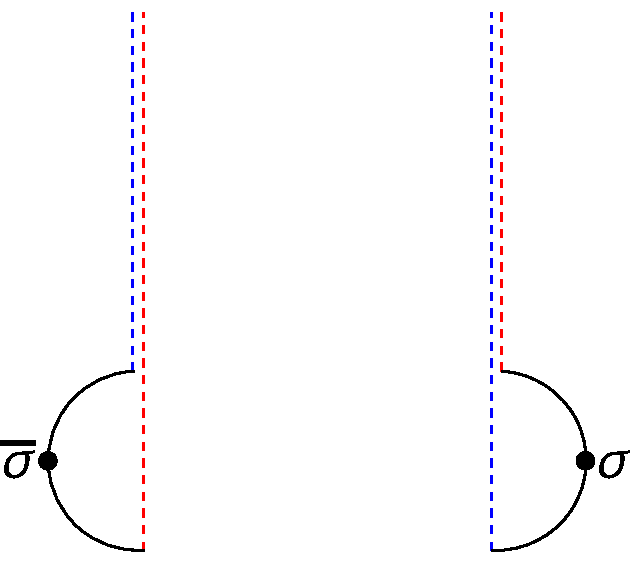
\includegraphics[width=.3\textwidth]{figures/flagstate.pdf}
\caption{Pictorial representation of the anti-flag state ${\overline\sigma}\textSFxxviii$ (left) and the flag state $\textSFl\sigma$ (right). $\textSFl\sigma$ is defined with the insertion of $[\sigma(0)]^{{\ell\over 2}h}$ on the right half disc of diameter $\ell$, where $h$ is the conformal map (\ref{hzdefz}) and ${\ell\over 2}$ is a rescaling factor, and glued to an infinitesimally thin semi-infinite strip, whose left edge (dashed blue) and right edge (dashed red, shifted upward by $\ell$) are identified with the two halves of the open string similarly to the sliver map (Figure \ref{fig:sliver}).}\label{fig:flagstate}
\end{figure}


The remaining nontrivial task is to find $\Sigma_{\rm pre}, \overline\Sigma_{\rm pre}$ that satisfy (\ref{sigmapreaa}). This can be achieved using a construction known as {\it flag states}. We begin with a pair of matter interface operators $\sigma\in {\cal H}_{0*}^{\rm m}$, $\overline\sigma \in {\cal H}_{*0}^{\rm m}$, where the superscript m indicates matter BCFT Hilbert space, normalized such that $\langle\langle \overline\sigma | \sigma\rangle = 1$. We will also make the inconspicuous assumption that the zero weight component of the OPE $\overline\sigma \sigma$ is proportional to the identity boundary operator in BCFT$_*$.\footnote{This assumption is important when the matter sector of BCFT$_*$ has degenerate zero weight states, e.g. in the presence of Chan-Paton factors.}

The flag state associated with $\sigma$, which we denote by the suggestive symbol $\textSFl\sigma$, is defined similarly to the zero-width wedge state $\Omega^0$ in the sliver frame, except that the right semi-infinite edge is shifted upward by a certain length $\ell$, making room for the insertion of the state $\sigma$ along the vertical segment of length $\ell$, as indicated in the right of Figure \ref{fig:flagstate}. The anti-flag state ${\overline\sigma}\textSFxxviii$ is defined similarly by the left of Figure \ref{fig:flagstate}. 

The $*$-product of ${\overline\sigma}\textSFxxviii$ and $\textSFl\sigma$ produces a state that is defined by gluing the red edge in the left of Figure \ref{fig:flagstate} to the blue edge in the right of Figure \ref{fig:flagstate}, resulting in a disc that ``pinches off'' and leaving behind the identity string field $\mathtt{I}=\Omega^0$, namely
\ie
{\overline\sigma}\textSFxxviii * \textSFl\sigma = \mathtt{I}.
\fe
A more delicate relation that will be needed below, which relies crucially on $\sigma$ and $\overline\sigma$ being matter BCFT operators, is
\ie\label{sigmabsig}
{\overline\sigma}\textSFxxviii \mt{B} \textSFl\sigma= \mt{B}.
\fe
The tachyon vacuum string field (\ref{tvkbc}) can be expressed in a more general gauge as\footnote{Okawa, JHEP \textbf{04} (2006), 055 \cite{Okawa:2006vm}.}
\ie\label{psitmgeng}
\Psi_{\rm tv} = ( F(\mt{K}) )^{1\over 2} \mt{c} {\mt{B}\over H(\mt{K})} \mt{c} \left( F(\mt{K}) \right)^{1\over 2},
\fe
where $F(x)$ is a suitable real analytic function, and $H(x) \equiv {1-F(x)\over x}$. For instance, denoting (\ref{tvkbc}) as $\Psi_{\rm tv}^{s}$, the gauge transformed string field $\Psi_{\rm tv} = (\mt{I}+\mt{K})^{-{1\over 2}} (Q_B + \Psi_{\rm tv}^{s})  (\mt{I}+\mt{K})^{1\over 2}$ gives (\ref{psitmgeng}) in the special case $F(x) = H(x) = (1+x)^{-1}$. The homotopy operator $\mt{A}$ can now be expressed as
\ie
\mt{A} = \mt{B} H(\mt{K}).
\fe
$\Sigma_{\rm pre}$ and $\overline\Sigma_{\rm pre}$ can be constructed as
\ie
\Sigma_{\rm pre} = (H(\mt{K}))^{-{1\over 2}}  \textSFl\sigma  (H(\mt{K}))^{{1\over 2}} ,~~~~ \overline\Sigma_{\rm pre} = (H(\mt{K}))^{{1\over 2}}  {\overline\sigma}\textSFxxviii   (H(\mt{K}))^{-{1\over 2}}.
\fe
Indeed, using (\ref{sigmabsig}), we have
\ie
\overline\Sigma_{\rm pre} \mathtt{A} \Sigma_{\rm pre} = (H(\mt{K}))^{{1\over 2}} {\overline\sigma}\textSFxxviii \mt{B} \textSFl\sigma (H(\mt{K}))^{{1\over 2}} =  (H(\mt{K}))^{{1\over 2}}  \mt{B}  (H(\mt{K}))^{{1\over 2}} = \mt{A},
\fe
thereby satisfying (\ref{sigmapreaa}).

As the OSFT is expected to capture all open string excitations on a D-brane, it should in particular be able to describe the D-brane folding onto itself. A striking feature of the Erler-Maccaferri solution (\ref{psiintertw}) is that it allows for describing multiple D-branes as a solution of the OSFT based on a single D-brane. For instance, we may take BCFT$_*$ to be BCFT$_0$ tensored with the $U(k)$ Chan-Paton factor. In this case, the interface operator $\sigma \in {\cal H}_{0*}\sim {\cal H}_{00}\otimes \mathbb{C}^k$ can be represented as a row vector $(\sigma_1, \cdots, \sigma_k)$ where each $\sigma_i$ is a boundary operator of BCFT$_0$, and $\overline\sigma\in{\cal H}_{*0}$ a constant column vector $(\overline\sigma_1, \cdots, \overline\sigma_k)$. We must impose the condition that the zero weight component of $\overline\sigma \sigma$, now represented as a $k\times k$ matrix, to be proportional to the identity matrix operator. In other words, we require the zero weight component of the OPE $\overline\sigma_i(y) \sigma_j(0)$ to be proportional to $\delta_{ij}$ in BCFT$_0$, and impose the orthogonality condition 
\ie
\langle\langle \overline\sigma_i |\sigma_j\rangle = \delta_{ij}.
\fe
This requires taking $\sigma_i$ to be nontrivial boundary operators, but is not hard to satisfy in a general BCFT$_0$. The resulting string field solution then represents $k$ coincident D-branes. 








\subsection{BV formulation of quantum open+closed string field theory}
\label{sec:ocsft}

Generalizing the quantum closed SFT introduced in section \ref{bvsftsec}, the quantum theory of closed string fields coupled to open string fields on a D-brane can be formulated based on the BV field space
\ie
{\cal H}^c\oplus {\cal H}^o,
\fe
where ${\cal H}^c={\cal H}_0$ is the closed string field space defined in (\ref{blcon}), and ${\cal H}^o$ is the space of open string fields as in section \ref{sec:bvbosft}. The quantum BV action takes the form
\ie\label{oncact}
S[\Psi_c, \Psi_o] = {1\over 2} \langle\langle\Psi_c|c_0^- Q_B|\Psi_c\rangle + {1\over 2} \langle\langle \Psi_o | Q_B |\Psi_o\rangle + \sum_{h, n; b,m} {1\over n! m!} \{\Psi_c^{\otimes n}; \Psi_o^{\otimes m} \}_{h,n;b,m},
\fe
where $\{\Psi_c^{\otimes n}; \Psi_o^{\otimes m} \}_{h,n;b,m}$ is the string vertex of genus $h$, $b$ boundary components, that involve $n$ closed string fields $\Psi_c$ and $m$ open string fields $\Psi_o$, constructed as
\ie\label{oncvert}
\{\Psi_c^{\otimes n}; \Psi_o^{\otimes m} \}_{h,n;b,m} = - {\cal N}_{h,n;b,m} \int_{\Gamma_{h,n; b,m}} \Omega[\Psi_c^{\otimes n}; \Psi_o^{\otimes m}]
\fe
for $d\equiv 6h-6+3b+2n+m\geq 0$, except for the case $(h,n;b,m)=(0,1;1,0)$, i.e. the disc with one bulk puncture, which will be treated separately below. Here $\Omega$ is a differential form on the fiber bundle ${\cal P}_{h,n;b,m} \to {\cal M}_{h,m;b,m}$ that parameterizes the punctured Riemann surface with boundary $\Sigma$ together with the choice of coordinate systems around the bulk (closed string) and boundary (open string) punctures, defined similarly to (\ref{omegaopencl}) as
\ie\label{omegaopenclsft}
\Omega[\Psi_c^{\otimes n}; \Psi_o^{\otimes m}] = \left\langle e^{\cal B} \prod_{i=1}^n \left[\Psi_c(0)\right]^{f_i} \prod_{j=1}^m \left[\Psi_o(0)\right]^{g_j} \right\rangle_{\Sigma},
\fe
where $f_i$ and $g_j$ are the coordinate maps associated with the bulk and boundary punctures. $\Gamma_{h,n;b,m}$ are $d$-dimensional chains in ${\cal P}_{h,n;b,m}$ that satisfy a set of geometric master equations generalizing (\ref{stringvcomp}). The normalization factor ${\cal N}_{h,n;b,m}$ is taken to be
\ie
{\cal N}_{h,n;b,m} = \Big( {e^{\pi i\over 2}\over 2\pi} \Big)^{3h-3+n+{3\over 2} b + {3\over 4} m} .
\fe
Our convention is such that in the absence of boundaries, i.e. when $b=m=0$, (\ref{oncvert}) reduces to the closed string vertex (\ref{psibracketg}).\footnote{Note that the normalization of the open string field $\Psi_o$ appearing in (\ref{oncact}), (\ref{oncvert}) differs from that of section \ref{sec:bvbosft} by a factor $(2\pi)^{3\over 4}$.}

In the exceptional case of the disc with one bulk puncture, we demand that the local coordinate $w$ at the puncture to be such that the boundary of the disc is located at $|w|=r$, for a constant $r> 1$. The corresponding disc 1-string vertex is then constructed as
\ie\label{disconv}
\{ \Psi_c \}_{0,1;1,0} = {1\over 2\pi i} {\cal N}_{0,1;1,0} \langle\langle \Psi_c | r^{-L_0^+} c_0^- |B\rangle,
\fe
where $|B\rangle$ is the D-brane boundary state. The normalization of (\ref{disconv}) is fixed by consistency with the BV master equation. Consider for instance the component of the BV master equation associated with the disc 2-closed-string amplitude,
\ie\label{qbopclsf}
& \{ Q_B \Psi_c^{\otimes 2} \}_{0,2;1,0} + \sum_I \{\Psi_c\otimes \psi^{I\ddagger}\}_{0,1;1,1} \{ \psi_{I}\otimes \Psi_c \}_{0,1;1,1}
\\
& + \Big[ \sum_I  \{ \Psi_c^{\otimes 2}\otimes \phi^{I\ddagger} \}_{0,3;0,0} \{\phi_I\}_{0,1;1,0} + (\phi^{I\ddagger}\leftrightarrow \phi_I) \Big] = 0,
\fe
where $(\phi_I, \phi^{I\dagger})$ are dual bases of $({\cal H}^{c,-},{\cal H}^{c,+})$ defined as in (\ref{basisinnnersft}), and $(\psi_I, \psi^{I\dagger})$ are dual bases of $({\cal H}^{o,-},{\cal H}^{o,+})$ defined as in (\ref{osftdualbas}). The first term on the LHS can be written as
\ie
\{ Q_B \Psi_c^{\otimes 2} \}_{0,2;1,0} = - {\cal N}_{0,2;1,0} \int_{\Gamma_{0,2;1,0}} \Omega[Q_B \Psi_c^{\otimes 2}]
= - {\cal N}_{0,2;1,0} \int_{\partial\Gamma_{0,2;1,0}} \Omega[ \Psi_c^{\otimes 2}],
\fe
where $\Gamma_{0,2;1,0}$ is a 1-dimensional chain whose boundary consists of 2 points. We can write 
\ie
\partial\Gamma_{0,2;1,0} = - \C_o - \C_c,
\fe
where $\C_o$ is obtained from joining a pair of punctured discs (as the point in $\Gamma_{0,1;1,0}$) via an open string plumbing fixture, and $\C_c$ is obtained from joining a 3-puncture sphere (as the point in $\Gamma_{0,3;0,0}$) with a 1-punctured disc via a closed string plumbing fixture. These contributions cancel against the second and third term on the LHS of (\ref{qbopclsf}) provided that the relevant coordinate maps are consistent with the plumbing fixture. For instance, the matching condition over $\C_c$ requires
\ie{}
& -{\cal N}_{0,2;1,0} \left\langle [\Psi_c(0)]^{f_1^{0,2;1,0}} [\Psi_c(0)]^{f_2^{0,2;1,0}} \right\rangle_{D^2} 
\\
& = { {\cal N}_{0,1;1,0}\over 2\pi i} \sum_I \left\langle [\Psi_c(0)]^{f_1^{0,3}} [\Psi_c(0)]^{f_2^{0,3}} [\phi^{I\ddagger}(0)]^{f_3^{0,3}} \right\rangle_{S^2} \langle\langle \phi_I| c_0^- r^{-L_0^+} |B\rangle + (\phi^{I\ddagger}\leftrightarrow \phi_I) ,
\fe
which is satisfied provided the coordinate maps are related by 
\ie
f_i^{0,2;1,0}(w) = r^{-1} ((f_3^{0,3})^{-1}\circ  f_i^{0,3}) (w), ~~~~i=1,2.
\fe

Let $D_i$ be the unit disc with respect to the local coordinate around the $i$-th bulk puncture, $D_j^o$ be the unit half disc with respect to the local coordinate around the $j$-th boundary puncture, and $\Sigma' = \Sigma \backslash (\sqcup_i D_i \sqcup_j D_j^o)$ be the worldsheet surface with the unit (half) discs containing the punctures removed. A set of open+closed string vertices for all $(h,n;b,m)$ can be constructed using the hyperbolic Hermitian metric of Gaussian curvature $-1$ on $\Sigma'$, subject to

\noindent 1. each $\partial D_i$ is a closed geodesic of length $L_c$, and all closed geodesics in $\Sigma'$ have length $\geq L_c$;

\noindent 2. each $\partial D_j^o\cap \Sigma'$ is an open geodesic of length $L_o$, and all open geodesics in $\Sigma'$ with ends on $\partial \Sigma$ that are not homotopic to a boundary segment have length $\leq L_o$;

\noindent 3. $\partial \Sigma \backslash \sqcup_j \partial D_j^o$ consists of geodesic segments that meet $\partial D_j^o\cap \Sigma'$ at right angles.

It can be shown that these conditions specify a consistent set of string vertices provided $L_c$ and $L_o$ obey\footnote{Cho,
JHEP \textbf{05} (2020), 046 \cite{Cho:2019anu}.}
\ie
0 < L_c \leq L_*', ~~~~ \sinh(L_c) \sinh(L_o)\leq 1,
\fe
where $L_*'$ is the solution to $\sinh{L_*'\over 2} \sinh L_*' = 1$, whose numerical value is $L_*'\approx 1.21876$.\footnote{Note that $L_*'$ is smaller than the critical length $L_*$ (\ref{lstarc}) in the case of the purely closed string hyperbolic vertices.}

Interestingly, in the limit $L_o\to \infty$ with $L_c \leq (\sinh L_o)^{-1}$, the open string vertices reduce to that of Witten's cubic OSFT. That is, the only non-vanishing open string vertex is the disc 3-point vertex defined in (\ref{fffsd}). In this case, the $L$-loop Feynman diagrams built out of Witten's cubic open string vertex cover precisely the entire moduli space of Riemann surfaces with at least one boundary component and Euler characteristic $\chi = 1-L$,\footnote{This can also be shown by a generalization of the quadratic differential considered in section \ref{sec:cubicosft}; see Zwiebach, Commun. Math. Phys. \textbf{142} (1991), 193 \cite{Zwiebach:1990az}. } whereas the closed string field propagators only serve as counter terms that cancel the UV divergences from the open string loops. This would amount to a quantum OSFT based on the path integral over the open string fields only, with Witten's cubic OSFT action and a suitable UV regularization. In practice however, the quantum bosonic open+closed string theory suffers from either closed string tachyon instability, such as in critical bosonic string theory, or open string tachyon instability, as with the ZZ-brane in $c=1$ string theory, or massless closed string tadpole, as with FZZT-brane in $c=1$ string theory, all of which renders the conventional string perturbation theory ill-defined. Whether the quantum OSFT can be defined non-perturbatively remains an outstanding open question.






%However, This suggests that the path integral based on Witten's cubic OSFT and BV gauge fixing may well define a consistent quantum bosonic string field theory.





\subsection{Open+closed superstring field theory}
\label{sec:ocsftsup}

We now extend the closed type II superstring field theory formulated in section \ref{sec:bvcssft} to include open superstring fields on a (not necessarily BPS) D-brane. The space of open superstring fields ${\cal H}^o$ is defined as the space of states of the worldsheet SCFT on the strip subject to the D-brane boundary condition, that splits into its NS and R sector subspaces
\ie
{\cal H}^o = {\cal H}^o_{\rm NS}[-1] \oplus {\cal H}^o_{\rm R}[-\tfrac{1}{2}],
\fe
where the bracket notation indices the picture number assignment of the NS and R sector states. Note that in the case of the BPS D-brane, the construction of open string fields based on free boson and fermions is subject to the open string GSO projection, as described in section \ref{sec:bpsdbrane}. To write the kinetic term for the R sector fields, we will also need to introduce the auxiliary open superstring field space
\ie
{\cal H}^{o,{\rm aux}} =  {\cal H}^o_{\rm NS}[-1] \oplus {\cal H}^o_{\rm R}[-\tfrac{3}{2}].
\fe
${\cal H}^o\oplus {\cal H}^{o,{\rm aux}}$ is equipped with a BV symplectic structure, as follows. Splitting
\ie
{\cal H}^o = {\cal H}^{o,-} \oplus {\cal H}^{o,+},~~~~{\cal H}^{o,{\rm aux}} = {\cal H}^{o,{\rm aux},-} \oplus {\cal H}^{o,{\rm aux},+} ,
\fe
where the superscript $-$ stands for the subspace of ghost number\footnote{Here $N_{\rm gh}$ is defined as the open string analog of (\ref{ghnumsup}), which assigns charge $+1$ to $c,\C$, $-1$ to $b,\B$, and 0 to $e^{\A\phi}$.} $N_{\rm gh}\leq 1$, and the superscript $+$ stands for the subspace of $N_{\rm gh}\geq 2$, we consider a basis $|\varphi_I\rangle$ of ${\cal H}^{o,-}$ and its dual basis $|\widetilde\varphi^{I\ddagger}\rangle$ of ${\cal H}^{o,{\rm aux},+}$ that satisfy the BPZ inner product and completeness relation
\ie
& \langle\langle \widetilde\varphi^{I\ddagger}| \varphi_J\rangle = \delta^I_J, ~~~~\langle\langle \varphi_I| \widetilde\varphi^{J\ddagger}\rangle =  \delta_I^J,
\\
& \sum_I |\varphi_I\rangle \langle\langle \widetilde\varphi^{I\ddagger}|  = 1_{{\cal H}^{o,-}},~~~~ \sum_I |\widetilde\varphi^{I\ddagger}\rangle \langle\langle \varphi_I| =  1_{{\cal H}^{o,{\rm aux},+}}.
\fe
and similarly a basis $|\widetilde\varphi_I\rangle$ of ${\cal H}^{o,{\rm aux},-}$ and its dual basis $|\varphi^{I\ddagger}\rangle$ of ${\cal H}^{o,+}$. In terms of the expansion of the open superstring fields $\Psi_o\in {\cal H}^o$ and $\widetilde\Psi_o\in {\cal H}^{o,{\rm aux}}$,
\ie\label{psiexpansi}
& |\Psi_o\rangle - {1\over 2} {\cal G} |\widetilde\Psi_o\rangle = \sum_I  |\varphi_I\rangle \psi_o^I - \sum_I \widetilde\psi_{o,I}^\ddagger |\varphi^{I\ddagger}\rangle,
\\
& |\widetilde\Psi_o \rangle = \sum_I  |\widetilde\varphi_I\rangle\widetilde\psi_o^I - \sum_I \psi_{o,I}^\ddagger |\widetilde\varphi^{I\ddagger}\rangle,
\fe
where ${\cal G}$ is the open string (or holomorphic, by the doubling trick) version of the picture-adjusting operator (\ref{pictureadjustop}), the BV field/anti-field pairing is defined via the symplectic form
\ie
\omega = \sum_I d\psi_{o,I}^\ddagger \wedge d\psi_o^I + \sum_I d\widetilde\psi_{o,I}^\ddagger \wedge d\widetilde\psi_o^I .
\fe
The BV action functional of open+closed superstring theory, extending the closed string field action (\ref{bvsftfnlsuper}), takes form
\ie\label{bvsftfnlsuperoc}
S[\Psi_c,\widetilde\Psi_c;\Psi_o,\wt\Psi_o] & = -{1\over 2} \langle\langle \widetilde\Psi_c | c_0^- Q_B {\cal G} |\widetilde\Psi_c \rangle + \langle\langle \widetilde\Psi_c |c_0^- Q_B|\Psi_c \rangle
-{1\over 2} \langle\langle \widetilde\Psi_o | Q_B {\cal G} |\widetilde\Psi_o\rangle + \langle\langle \widetilde\Psi_o | Q_B|\Psi_o\rangle
\\
&~~~ + \{ \wt\Psi_c \}_{D^2} +  {\sum_{h,n;b,m}}'  {1\over n! m!} \{\Psi_c^{\otimes n}; \Psi_o^{\otimes m}\}_{h,n;b,m},
\fe
where the summation over $(h,n;b,m)$ in the last term excludes the case $(0,1;1,0)$, namely the disc closed string 1-point vertex, which is replaced with the disc vertex associated with the auxiliary closed string field $\{ \wt\Psi_c \}_{D^2}$. The latter is constructed analogously to the bosonic string case (\ref{disconv}),
\ie\label{disconeptsup}
\{ \wt\Psi_c \}_{D^2} = {1\over 2\pi i} {\cal N}_{0,1;1,0} \langle\langle \wt\Psi_c | r^{-L_0^+} c_0^- {\cal G} |B\rangle,
\fe
where the boundary of the disc is located at $|w|=r \,(> 1$) in terms of the local coordinate $w$ associated with the puncture, and $|B\rangle$ is the D-brane boundary state (averaged over boundary spin structure assignment as in (\ref{dpavg})). 

To construct the open+closed superstring vertex $\{\Psi_c^{\otimes n}; \Psi_o^{\otimes m} \}_{h,n;b,m}$, we consider the fiber bundle $\pi:\widehat{\cal Q}_{h,n;b,m}\to {\cal M}_{h,n;b,m}$ that extends ${\cal Y}_{h,n;b,m}\to {\cal M}_{h,n;b,m}$ (introduced in section \ref{sec:openclosedpertsuper}) by including the coordinate maps $f_i, g_j$ associated with the bulk and boundary punctures, modulo the constant phase rotation of the local coordinates around the bulk punctures as in (\ref{qnquot}), and define the differential form $\Omega$ on $\widehat{\cal Q}_{h,n;b,m}$ that generalizes (\ref{omegassft}),
\ie
\Omega[\Psi_c^{\otimes n}; \Psi_o^{\otimes m}] = \left\langle e^{\pi^*{\cal B}} \prod_{a=1}^{d_o} \big[ {\cal X}(x_a) - d\xi(x_a) \big] \prod_{\widetilde a=1}^{\widetilde d_o} \big[ \widetilde{\cal X}(\bar{\widetilde x}_{\widetilde a}) - d\widetilde\xi(\bar{\widetilde x}_{\widetilde a})\big] \prod_{i=1}^n \left[ \Psi_c(0) \right]^{f_i} \prod_{j=1}^m \left[ \Psi_o(0) \right]^{g_j} \right\rangle_{\Sigma, \epsilon}.
\fe
Here the total number of holomorphic and anti-holomorphic PCOs is $d_o+\wt d_o = 4h-4+2b+n_{\rm NS} + {n_{\rm R}\over 2}$, where $n_{\rm NS/R}$ counts the total number of holomorphic, anti-holomorphic, and boundary punctures of NS/R type. Note that in the presence of a boundary, $d_o$ and $\wt d_o$ need not be separately fixed along a PCO contour. The open+closed superstring vertex, generalizing the closed string case (\ref{sssftvert}), is given by
\ie\label{oncvert}
\{\Psi_c^{\otimes n}; \Psi_o^{\otimes m} \}_{h,n;b,m} = - {{\cal N}_{h,n;b,m}\over 2^{2h+b }} \int_{\Upsilon_{h,n; b,m}} \Omega[\Psi_c^{\otimes n}; \Psi_o^{\otimes m}],
\fe
where $\Upsilon_{h,n; b,m}$ is a $(6h-6+3b+n_{\rm NS}+n_{\rm R})$-dimensional chain in $\widehat{\cal Q}_{h,n;b,m}$ that is symmetric with respect to exchange of any pair of punctures of the same (bulk/boundary; NS/R) type, and satisfy geometric master equations that generalize (\ref{geommassuper}) to include open string plumbing.

At the leading order in perturbation theory, after eliminating the auxiliary field $\wt\Psi_c$, the linearized equation of motion for the closed string field $\Psi_c$, reads
\ie\label{qbpsilinsup}
Q_B|\Psi_c\rangle = - {{\cal N}_{0,1;1,0}\over 2\pi i} r^{-L_0^+} {\cal G} |B\rangle.
\fe
That is, the vacuum configuration of the open+closed SFT involves turning on the closed string field sourced by the D-brane. Note that while ${\cal G} |B\rangle$ is $Q_B$-closed, it may in principle represent a nontrivial $Q_B$-cohomology class (analogous to a massless tadpole) that obstructs the solution to (\ref{qbpsilinsup}).\footnote{This occurs for the D9-brane in type IIB string theory, which will be considered in section \ref{sec:typei}.} Such obstructions are absent if $L_0^+$ is invertible on $|B\rangle$, in which case we can solve (\ref{qbpsilinsup}) in the Siegel gauge with
\ie\label{qbpsilinsupsol}
|\Psi_c\rangle =  - {{\cal N}_{0,1;1,0}\over 2\pi i} r^{-L_0^+} {b_0^+\over L_0^+}{\cal G} |B\rangle.
\fe
For a flat BPS D$p$-brane in Minkowskian spacetime, for instance, (\ref{qbpsilinsupsol}) produces a closed string field profile that is similar to the Newton potential sourced by a {\it smeared} mass (or the gauge field sourced by a smeared charge), due to the factor $r^{-L_0^+}$ on the RHS (\ref{qbpsilinsupsol}) which regularizes the closed string field at the location of the D-brane. 





\newpage


\section{D-instantons}
\label{sec:dinsteffects}

\subsection{The effect of D-instantons}

The construction of the string S-matrix based on the worldsheet path integral and closed SFT has thus far been organized according to the genus expansion, and is perturbative with respect to the string coupling $g_s$. 
Such a perturbative expansion is expected to yield an asymptotic series that is not convergent at any nonzero value of the string coupling.\footnote{Gross and Periwal, Phys. Rev. Lett. \textbf{60} (1988), 2105 \cite{Gross:1988ib}.} A complete formulation of string theory should include D-branes, perhaps in the form of open+closed SFT. While the latter has only been defined at the level of perturbation theory in sections \ref{sec:ocsft} and \ref{sec:ocsftsup}, one expects that any reasonable non-perturbative completion of the D-brane path integral should contain saddle points corresponding to Euclidean D-brane solutions that are localized in spacetime, similarly to the bounce or instanton solutions of the Euclidean equation of motion that play the role of non-perturbative saddle points in the path integral formulation of quantum field theory. Such Euclidean D-brane solutions, or ``D-instantons'', are expected to mediate non-perturbative corrections to string amplitudes of order $\exp(-C/g_s)$ where $C$ does not scale with $g_s$. The simplest examples of D-instantons include the ZZ-instanton in $c=1$ string theory (section \ref{sec:zzinst}) and the BPS D$(-1)$-brane in type IIB string theory (section \ref{sec:iibdinst}). 

Our basic postulate is that the closed string scattering amplitude takes the form
\ie
{\cal A} = {\cal A}^{\rm pert} + {\cal A}^{\rm D- inst} + \cdots,
\fe
where ${\cal A}^{\rm pert}$ stands for the perturbative amplitude, ${\cal A}^{\rm D-inst}$ the contribution from worldsheets with boundaries that are subject to the D-instanton boundary conditions, and $\cdots$ stands for higher order non-perturbative effects, such as gravitational instanton contributions which are expected to be of order $\exp(-C/g_s^2)$. Strictly speaking, to define ${\cal A}^{\rm pert}$ requires summing up the perturbative series in $g_s$, e.g. through Borel resummation with a suitable integration contour on the Borel plane (Appendix \ref{sec:borel}), and the non-perturbative corrections are subject to potential ambiguities of the resummation procedure. In this chapter we will focus on examples where the perturbative amplitude can be Borel-resummed (as in $c=1$ string theory) or truncates at a finite order (as for BPS-protected amplitudes in superstring theory), in which case the D-instanton corrections are unambiguously defined and will turn out to be essential for the consistency of various string dualities.


Generally, a D-instanton comes in a continuous family that is parameterized by the moduli space ${\cal M}_{\rm D-inst}$ of exactly marginal deformations of the corresponding worldsheet boundary condition. By analogy with the on-shell formulation of string perturbation theory, one may anticipate the D-instanton contribution to the closed string amplitude to be of the form
\ie\label{ainstgend}
{\cal A}^{\rm D-inst}[V_1,\cdots,V_n] = \int_{{\cal M}_{\rm D-inst}} d\mu(x) {\cal A}_x[V_1,\cdots,V_n ],
\fe
where ${\cal A}_x$ is computed by the path integral over worldsheet with boundaries, whose boundary condition is specified by $x\in {\cal M}_{\rm D-inst}$, with insertions of closed string vertex operators $V_1,\cdots,V_n$, and $d\mu(x)$ is a suitable measure on ${\cal M}_{\rm D-inst}$. Note that the relevant worldsheet configuration can contain arbitrarily many connected components, provided that each of its connected component has a non-empty boundary. This is because a disconnected set of worldsheet diagrams subject to the {\it same} D-instanton boundary condition, upon integration over the D-instanton moduli space ${\cal M}_{\rm inst}$, nonetheless yields a contribution to the connected closed string amplitude. Accounting for the combinatorial factors associated with the large diffeomorphisms that permute different connected components of the worldsheet, ${\cal A}_x$ can be decomposed in terms of the connected worldsheets as
\ie\label{acdecom}
{\cal A}_x[V_1,\cdots,V_n] = \exp\left( \sum_{h\geq 0, b\geq 1} A^{\rm c}_{x|h,b} [\emptyset] \right) \sum_{\sqcup_I \A_I = \{1,\cdots,n\}}  \prod_I \sum_{h\geq 0, b\geq 1} {\cal A}_{x|h,b}^c[\{V_i\}_{i\in \A_I}].
\fe
The RHS involves a sum over unordered partitions of $\{1,\cdots,n\}$ into the index subsets $\A_I$, and $A^{\rm c}_{x|h,b}[\{V_i\}_{i\in \A_I}]$ is the contribution from a single connected component of the worldsheet of genus $h$, $b$ boundaries, and insertions of closed string vertex operators $V_i$ for $i\in \A_I$.  $A^{\rm c}_{x|h,b} [\emptyset]$ stands for the contributions from a connected component of the worldsheet with boundaries but no closed string insertions, which exponentiates into the prefactor. In particular, $A^{\rm c}_{x|0,1} [\emptyset]$ which is formally\footnote{Strictly speaking, the ``empty disc'' amplitude is undefined in the formalism of open+closed perturbation theory introduced in sections \ref{sec:openclosedpert}. An appropriate definition can be made by relating its derivative with respect to the dilaton background value to the disc amplitude with a dilaton vertex operator insertion. Such relations, more generally known as the ``dilaton theorem'', are rigorously established in the string field theory framework by Bergman and Zwiebach, Nucl. Phys. B \textbf{441} (1995), 76 \cite{Bergman:1994qq}. } of order $g_s^{-1}$ can be interpreted as minus the classical action of the D-instanton, whereas $A^{\rm c}_{x|h,b} [\emptyset]$ with $b\geq 2$ or $h\geq 1$ represent quantum corrections to the D-instanton effective action or equivalently to the measure factor on the D-instanton moduli space.

Following the rules of open+closed string perturbation theory, say in the bosonic string case, one may expect $A^{\rm c}_{x|h,b}[V_1,\cdots,V_n]$ to be given by
\ie\label{naiveacexp}
A^{\rm c}_{x|h,b}[V_1,\cdots,V_n] = N_{h,n;b,0} \int_{{\cal M}_{h,n;b,0}} \left\langle e^{\cal B} \prod_{i=1}^n {\cal V}_i \right\rangle_{\Sigma, x},
\fe
analogously to (\ref{openampbos}) except that the D-brane boundary condition is replaced by that of the D-instanton, and that there are no open string vertex operator insertions. As in the on-shell string perturbation theory, the RHS of (\ref{naiveacexp}) generally suffers from divergences near the boundary of the moduli space ${\cal M}_{h,n;b,0}$ due to the exchange of on-shell open string modes. However, unlike the open+closed string amplitude on a D-brane, where such divergences may be regularized by analytic continuation with respect to the momenta of the (external as well as internal) string states, the open string modes on the D-instanton carry no momentum and their divergent propagators cannot be regularized by analytic continuation in momenta. Similar open string divergences plague the empty worldsheet diagrams $A^{\rm c}_{x|h,b} [\emptyset]$, whose ambiguities are tied to that of the measure factor $d\mu(x)$ on the D-instanton moduli space. 

\begin{figure}[h!]
\centering
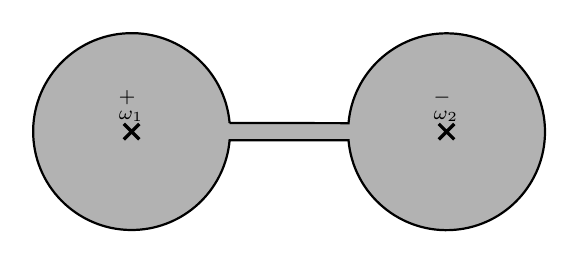
\begin{tikzpicture}
\filldraw[color=black, fill=black!30, thick] (1.245,0.11) arc (5:355:1.25) -- (4-1.245,-0.11) arc (185:360:1.25) arc (0:175:1.25) -- (1.245,0.11);
\draw (0,0) node[cross=4pt, very thick] {};
\draw (0,0) node[above] {$\cV^{+}_{\omega_1}$};
\draw (4,0) node[cross=4pt, very thick] {};
\draw (4,0) node[above] {$\cV^{-}_{\omega_2}$};
\end{tikzpicture}
\medskip
\begin{tabular}{c c c}
& & \\
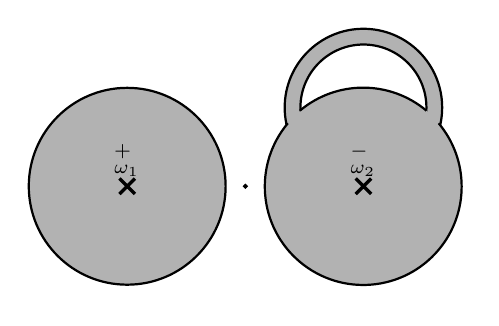
\begin{tikzpicture}
\filldraw[color=black, fill=black!30, thick] (-3,0) circle (1.25);
\draw (-3,0) node[cross=4pt, very thick] {};
\draw (-3,0) node[above] {$\cV^{+}_{\omega_1}$};
\draw[fill] (-1.5,0) circle [radius=0.025];
\filldraw[color=black, fill=black!30, thick] (0,1) circle (1);
\filldraw[color=black, fill=white, thick] (0,1) circle (0.8);
\path [fill=black!30] (0,0) circle (1.25);
\draw [thick] (0.80,0.96) arc (50:180-50:1.25);
\draw [thick] (-0.96,0.80) arc (140:400:1.25);
\draw (0,0) node[cross=4pt, very thick] {};
\draw (0,0) node[above] {$\cV^{-}_{\omega_2}$};
\end{tikzpicture}
& $~~$ &
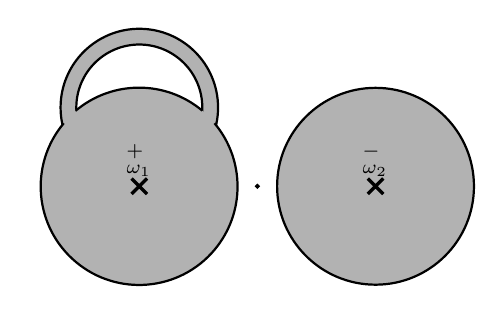
\begin{tikzpicture}
\filldraw[color=black, fill=black!30, thick] (0,1) circle (1);
\filldraw[color=black, fill=white, thick] (0,1) circle (0.8);
\path [fill=black!30] (0,0) circle (1.25);
\draw [thick] (0.80,0.96) arc (50:180-50:1.25);
\draw [thick] (-0.96,0.80) arc (140:400:1.25);
\draw (0,0) node[cross=4pt, very thick] {};
\draw (0,0) node[above] {$\cV^{+}_{\omega_1}$};
\draw[fill] (1.5,0) circle [radius=0.025];
\filldraw[color=black, fill=black!30, thick] (3,0) circle (1.25);
\draw (3,0) node[cross=4pt, very thick] {};
\draw (3,0) node[above] {$\cV^{-}_{\omega_2}$};
\end{tikzpicture}
\end{tabular}
\caption{Degeneration limit of worldsheet diagrams that leads to logarithmic divergences due to propagation of the open string collective modes (e.g. on a ZZ-instanton considered in section \ref{sec:zzinst}). Formally, the divergences cancel in the sum of the three diagrams, but finite ambiguities remain in the on-shell approach.}
\label{fig:divlimit}
\end{figure}

In sections \ref{sec:zzinst} and \ref{sec:iibdinst}, we will adopt the naive on-shell approach to D-instantons in the bosonic $c=1$ string theory and type IIB string theory respectively, where the open string divergences are handled simply by cutting off the near-boundary regions of the moduli space. This prescription, while somewhat ad hoc, turns out to capture the correct leading order results up to certain counter term ambiguities. These ambiguities will be resolved through the open+closed string field theory formulation of D-instantons in section \ref{sec:dinstsft}.


\subsection{D-instantons in $c=1$ string theory}
\label{sec:zzinst}

The $c=1$ string theory admits a D-instanton that is defined by the ZZ boundary condition in the Liouville CFT (section \ref{sec:zzfzzt}) and Dirichlet boundary condition in the noncompact free boson CFT that describes Euclidean time, which we refer to as the ZZ-instanton.\footnote{The analogous construction with the FZZT boundary condition would have infinite action and would not mediate closed string scattering.} The action of the ZZ-instanton $S_{\rm ZZ}$ is related to the mass of the ZZ-brane (\ref{szzactmas}) by\footnote{Note that our convention for $g_s$ in $c=1$ string theory differs from that of Balthazar, Rodriguez, Yin, JHEP \textbf{05} (2023), 048 \cite{Balthazar:2019rnh} by a factor of 2.}
\ie\label{szzact}
S_{\rm ZZ} = 2\pi \sqrt{\A'} M_{\rm ZZ} = {1\over 2g_s}.
\fe
In the dual matrix quantum mechanics (MQM) description, a natural interpretation of the ZZ-instanton is that the Euclidean bounce solution of a single eigenvalue/fermion (Appendix \ref{sec:bounce}) which mediates non-perturbative effects in the scattering of the fermion or the collective modes of the fermi surface. Indeed, the action of the bounce at the fermi energy $H \equiv {1\over 2}(p^2-x^2)=-\mu$ is 
\ie
S_{\rm bounce} = 2 \int_{-\sqrt{2\mu}}^{\sqrt{2\mu}} dx\sqrt{2\mu - x^2} = 2\pi \mu,
\fe
which precisely agrees with (\ref{szzact}) with the identification $\mu = {1\over 4\pi g_s}$.

The non-perturbative corrections to the closed string amplitude mediated by the ZZ-instanton is expected to render the closed string S-matrix $S_c$ non-unitary, due to the tunneling to the ``wrong side'' of the potential in the MQM description. That is, one expects the expectation value of $1-S_c^\dagger S_c$ to give the probability of closed string states turning into other types of asymptotic states in $c=1$ string theory, such as ZZ-branes with open string tachyon rolling to the ``wrong side'' of the tachyon potential. In particular, the $1\to n$ S-matrix element (\ref{sacone}) obeys a non-perturbative unitarity relation of the form
\ie\label{oneminusp}
\sum_{n=1}^\infty \int_{\omega_i\geq 0} \prod_{i=1}^n {d\omega_i\over \omega_i} { |{\cal A}(\omega_1,\cdots,\omega_n)|^2\over \omega_1+\cdots+\omega_n} = 1 - P,
\fe
where $P$ is the probability of a single closed string turning into non-perturbative objects that are not closed strings.


\begin{figure}[h!]
\centering
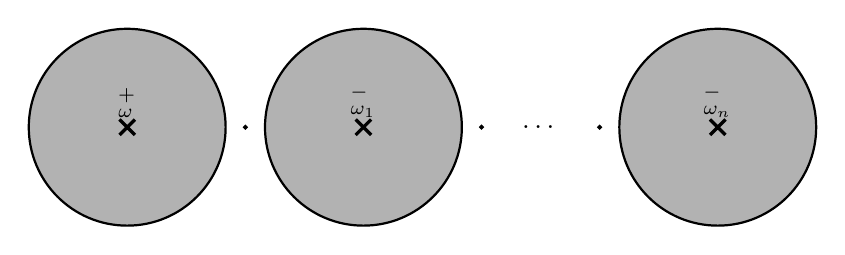
\begin{tikzpicture}
\filldraw[color=black, fill=black!30, thick] (0,0) circle (1.25);
\draw (0,0) node[cross=4pt, very thick] {};
\draw (0,0) node[above] {$\cV^{+}_{\omega}$};
\draw[fill] (1.5,0) circle [radius=0.025];
\filldraw[color=black, fill=black!30, thick] (3,0) circle (1.25);
\draw (3,0) node[cross=4pt, very thick] {};
\draw (3,0) node[above] {$\cV^{-}_{\omega_1}$};
\draw[fill] (4.5,0) circle [radius=0.025];
\node at (5.25,0) {$\dots$};
\draw[fill] (6,0) circle [radius=0.025];
\filldraw[color=black, fill=black!30, thick] (7.5,0) circle (1.25);
\draw (7.5,0) node[cross=4pt, very thick] {};
\draw (7.5,0) node[above] {$\cV^{-}_{\omega_n}$};
\end{tikzpicture}
\caption{Worldsheet diagram that computes the leading non-perturbative correction to the closed string $1\to n$ amplitude, of order $e^{-S_{\rm ZZ}}$, mediated by a single ZZ-instanton.}
\label{fig:LO1ton}
\end{figure}



The leading contribution of a ZZ-instanton to the $1\to n$ closed string amplitude is
\ie\label{sinstconef}
S^{\rm inst}(\omega_1, \cdots, \omega_n; \omega) = i {\cal N}^{\rm inst} e^{-S_{\rm ZZ}} \int_{-\infty}^\infty dx^0 \left\{ {\cal V}_\omega^+ \right\}_{D^2, x^0} \prod_{i=1}^n \left\{ {\cal V}_{\omega_i}^- \right\}_{D^2, x^0},
\fe
where ${\cal N}^{\rm inst}$ is an overall normalization constant associated with the ZZ-instanton. The relevant disc 1-point amplitude $\left\{ {\cal V} \right\}_{D^2, x^0}$, subject to the boundary condition that corresponds to a ZZ-instanton at time $x^0$, follows from the on-shell limit of (\ref{disconv}) and is evaluated as
\ie
\left\{ {\cal V}_\omega^\pm \right\}_{D^2, x^0} = {1\over 2\pi} \left\langle c_0^- {\cal V}_\omega^\pm \right\rangle_{D^2, x^0} = {\wt  K_{D^2}\over 2\pi} e^{\pm i {\omega\over \sqrt{\A'}} x^0} \Psi^{\rm ZZ}(\tfrac{\omega}{2}),
\fe
where $\Psi^{\rm ZZ}$ is given by (\ref{psizz}), and the normalization constant $\wt K_{D^2}$ is obtained similarly to (\ref{ndtwon}), with $K_{S^2}$ replaced by $\wt K_{S^2}$ (\ref{wtkstwo}), and ${\cal N}_{{\rm D}p}$ replaced by ${\cal N}_D$ (\ref{nzeroneum}) associated with the Dirichlet boundary condition of the free boson $X^0$,
\ie
\wt K_{D^2} = (\wt K_{S^2})^{1\over 2} {\cal N}_D =  2^{3\over 4} \sqrt{\pi} .
\fe
(\ref{sinstconef}) thus evaluates to
\ie\label{ninstampa}
i {\cal N}^{\rm inst} \sqrt{\A'} e^{-S_{\rm ZZ}} 2\pi \delta\Big(\omega - \sum_{i=1}^n \omega_i \Big) 2^{n+1} \sinh(\pi\omega) \prod_{i=1}^n \sinh(\pi\omega_i).
\fe
This result is in precise agreement with the leading non-perturbative correction to the $1\to n$ amplitude of particle-hole pairs in the dual MQM (Appendix \ref{sec:parthole}), provided the identification
\ie\label{ninstmatch}
{\cal N}^{\rm inst} = {i\over 8\pi^2 \sqrt{\A'}}.
\fe
Note that the overall sign of the ZZ-instanton contribution to ${\cal A}(\omega_1,\cdots,\omega_n)$ is negative, which is consistent with the positivity of the probability $P$ (\ref{oneminusp}) of scattering into non-closed string states.





\subsection{D-instantons in type IIB string theory}
\label{sec:iibdinst}

The type IIB superstring theory admits D-instantons in the form of BPS D$(-1)$-branes. The effective action of a BPS D$p$-brane derived in section \ref{sec:dbraneeffii} can be extended to the $p=-1$ case,\footnote{This can be derived using the D-instanton boundary state, or argued simply by applying T-duality on a Euclidean time circle.} yielding the (Euclidean) action of a single D$(-1)$-brane
\ie
S_{{\rm D}(-1)} = T_{-1} e^{-\Phi} - i \mu_{-1} C_0 = -2\pi i \tau,
\fe 
where $\tau \equiv \tau_1 + i \tau_2 = g_B^{-1}(C_0 + i e^{-\Phi})$, $C_0$ is the RR axion background field, and $g_B$ is the type IIB string coupling defined in (\ref{giibdef}). Likewise, the anti-D$(-1)$-brane has action
$S_{\overline{{\rm D}(-1)}} = 2\pi i \bar\tau$. A more general class of D-instantons is defined by the worldsheet boundary condition that is the direct sum of that of $n$ D$(-1)$-branes and $m$ anti-D$(-1)$-branes, which we will refer to as an $(n,m)$ D-instanton and has action $S_{(n,m)} = - 2\pi i (n\tau - m \bar\tau)$.

Importantly, while the perturbative type IIB closed string amplitudes are independent of the RR axion background or the value of $\tau_1$, the D-instantons mediate closed string interactions that are dependent on $\tau_1$ through the instanton action $S_{(n,m)}$ (when $n\not=m$). Moreover, the charge quantization of the D-instanton is such that constant shift of $\tau_1$ which is a symmetry to all orders in string perturbation theory is broken to the discrete shift symmetry $\tau_1\mapsto \tau_1+1$. The latter is part of the S-duality symmetry of type IIB string theory, as will be discussed in section \ref{sec:sduality}.

The simplest massless closed string amplitude affected by the D-instantons is that of four supergravitons, whose (NS,NS) component takes the form (\ref{nsnsfgen}). Accounting for possible non-perturbative dependence on $\tau_1$, we will replace the function $f(s,t;g_s)$ in (\ref{nsnsfgen}) with $f(s,t;\tau,\bar\tau)$, whose perturbative and D-instanton expansion is expected to be of the form
\ie\label{fstamp}
f(s,t;\tau,\bar\tau) = \sum_{h=0}^\infty \tau_2^{-2h} f_h(s,t) + \sum_{n,m} e^{2\pi i (n\tau - m \bar\tau)} f^{(n,m)}(s,t;\tau_2) + \cdots,
\fe
where $f_h$ represents the genus $h$ perturbative contribution, whose leading order results are given in (\ref{fstalpha}), $f^{(n,m))}$ represents the $(n,m)$ D-instanton contribution, and $\cdots$ stands for other possible non-perturbative corrections (such as gravitational instanton effects).


\begin{figure}[h!]
\centering
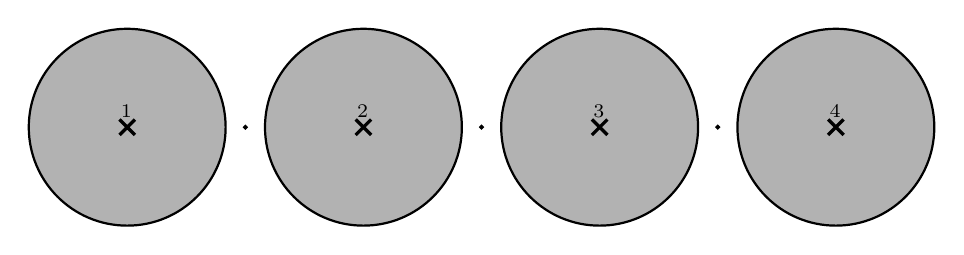
\begin{tikzpicture}
\filldraw[color=black, fill=black!30, thick] (0,0) circle (1.25);
\draw (0,0) node[cross=4pt, very thick] {};
\draw (0,0) node[above] {$\cV_1$};
\draw[fill] (1.5,0) circle [radius=0.025];
\filldraw[color=black, fill=black!30, thick] (3,0) circle (1.25);
\draw (3,0) node[cross=4pt, very thick] {};
\draw (3,0) node[above] {$\cV_2$};
\draw[fill] (4.5,0) circle [radius=0.025];
\filldraw[color=black, fill=black!30, thick] (6,0) circle (1.25);
\draw (6,0) node[cross=4pt, very thick] {};
\draw (6,0) node[above] {$\cV_3$};
\draw[fill] (7.5,0) circle [radius=0.025];
\filldraw[color=black, fill=black!30, thick] (9,0) circle (1.25);
\draw (9,0) node[cross=4pt, very thick] {};
\draw (9,0) node[above] {$\cV_4$};
\end{tikzpicture}
\caption{The leading D-instanton contribution to the four supergraviton amplitude is represented by the worldsheet diagram consisting of four discs, all of which are subject to the same D-instanton boundary condition labeled by $(x, \theta)$.}
\label{fig:LO1ton}
\end{figure}


We begin by considering the simplest nontrivial D-instanton contribution, namely the $(n,m)=(1,0)$ case (or similarly the $(0,1)$ case). At the leading order in the $1/\tau_2$ expansion, the relevant worldsheet diagram consists of four discs, each with the insertion of a supergraviton vertex operator ${\cal V}_i$, integrated over the D-instanton {\it supermoduli} space parameterized by the bosonic collective coordinate $x\in \mathbb{R}^{10}$ as well as the fermionic collective coordinates $\theta^\A$, the latter being Goldstinos associated with the 16 supersymmetries broken by the (${1\over 2}$-BPS) D-instanton,
\ie\label{leadingdinstiib}
{\cal A}^{(1,0)}[V_1,\cdots,V_4] = i N^{(1,0)} e^{2\pi i \tau} \int d^{10}x d^{16}\theta \prod_{i=1}^4 \left\{{\cal V}_i \right\}_{D^2, (x,\theta)}.
\fe
On the RHS, $N^{(1,0)}$ is an overall normalization constant to be determined,\footnote{Note that the contribution from the exponential of the empty annulus diagram has been absorbed into the normalization factor $N^{(1,0)}$.} and $\{\cdots\}_{D^2,(x,\theta)}$ stands for the disc amplitude subject to the D-instanton boundary condition parameterized by $(x,\theta)$. Setting $\theta=0$, the D-instanton boundary condition reduces to that of the D$(-1)$-brane, namely
\ie
\lim_{{\rm Im}(z) \to 0} X^\mu(z,\bar z) = x^\mu,~~~~ \lim_{{\rm Im}(z)\to 0} \left[\psi^\mu(z) + \hat\eta \wt \psi^\mu(\bar z) \right]=0,~~~~ \mu=0,\cdots,9,
\fe
in the notation of (\ref{imzxxdp}), (\ref{imzpsidp}). Turning on $\theta$ amounts to turning on an on-shell Ramond open string field on the D-instanton that corresponds to the marginal boundary vertex operator $\theta^\A j_\A$, where $j_\A = e^{-{\phi\over 2}} \Theta_\A$ is the spacetime supersymmetry current. This yields the relation
\ie\label{thetaxrela}
\Big( {\partial\over \partial \theta^\A} - i {\sqrt{\A'}\over 8} \Gamma^\mu_{\A\B}\theta^\B {\partial\over\partial x^\mu} \Big) \left\{ \cdots \right\}_{\Sigma, (x,\theta)} = \left\{ {\cal G} Q_\A ( \cdots )\right\}_{\Sigma, (x,\theta)} ,
\fe
where $Q_\A = \oint_{\partial \Sigma} {dz\over 2\pi i} j_\A(z)$ is the supercharge associated with $j_\A$, and ${\cal G}$ is the picture-adjusting operator defined by inserting the appropriate number of PCOs on each connected component of $\Sigma$. 
The additional term involving $x^\mu$-derivative on the LHS of (\ref{thetaxrela}) is needed for compatibility with the supersymmetry algebra (\ref{susyalgaa}). Integrating out $\theta^\A$ on the RHS of (\ref{leadingdinstiib}) and dropping total derivatives with respect to $x^\mu$ then yields
\ie\label{leadingdinstiibb}
{\cal A}^{(1,0)}[V_1,\cdots,V_4] = i N^{(1,0)} e^{2\pi i \tau} \int d^{10}x \left\{ {\cal G} \prod_{\A=1}^{16} Q_\A \prod_{i=1}^4{\cal V}_i\right\}_{\sqcup_{i=1}^4(D^2)_i,x},
\fe
where the ${\cal V}_i$'s are understood to be inserted on the four disjoint discs $D_i$.

The disc 1-point amplitudes appearing on the RHS of (\ref{leadingdinstiibb}) should be defined as the on-shell limit of (\ref{disconeptsup}), which handles the residual conformal Killing vector of the 1-punctured disc with an extra $c$ ghost insertion, and appropriately adjusts the picture number in the case of an (R,R) vertex operator insertion. A workaround that produces equivalent results is to relate the derivative of an amplitude with respect to the D-instanton moduli $x^\mu$ to the amplitude with an extra insertion of the open string mode that corresponds to the moduli deformation,\footnote{One may in principle treat $\theta$ deformation in similar manner, by representing it as inserting the Ramond open string vertex operator $cj_\A$. However, amplitudes with multiple such open string insertions are a priori singular, an issue that is evaded in (\ref{thetaxrela}).}
\ie\label{discderiv}
{\partial\over \partial x^\mu} \left\{ \cdots \right\}_{\Sigma, x} = \left\{ \cdots \otimes \Phi_{x^\mu} \right\}_{\Sigma, x},
\fe
where $\Phi_{x^\mu} = {1\over \pi}\sqrt{2\over \A'} c e^{-\phi} \psi_\mu$ is fixed by demanding its picture-raised version to agree with the marginal operator appearing in (\ref{exppsigdxx}). 



It will be useful to organize the type IIB supersymmetry algebra according to its $U(1)_R$ outer automorphism,\footnote{The $U(1)_R$ can be identified with a subgroup of the $SL(2,\mathbb{R})$ global symmetry of the 2-derivative type IIB supergravity, which is violated by the higher-derivative corrections in type IIB string theory.} under which 
\ie
Q_\A^\pm \equiv Q_\A \pm i \wt Q_\A
\fe
carries charge $\pm 1$. Importantly, the $(1,0)$ D-instanton preserves the supercharge $Q_\A^-$, whereas the $(0,1)$ D-instanton (i.e. anti-D-instanton) preserves the supercharge $Q_\A^+$.\footnote{This follows from the $p=-1$ case of (\ref{jalbdrycond}) with a further Wick rotation.} On the RHS of (\ref{leadingdinstiibb}), we may equivalently trade $Q_\A$  with the broken supercharge ${1\over 2} Q_\A^+$.

%Note that a priori, the supercharges $Q_\A$ and $\wt Q_\A$ associated with the holomorphic and anti-holomorphic currents $j_\A$ and $\wt j_\A$ are in the $(-{1\over 2},0)$ and $(0,-{1\over 2})$ picture respectively. The corresponding supersymmetry transformation of the on-shell vertex operators should be accompanied by the picture-adjusting operator ${\cal G}$ so as to maintain picture number $-1$ in the NS sector and $-{1\over 2}$ in the R sector.

The supergraviton multiplet at a given lightlike momentum $k^\mu$ is spanned by $2^8=256$ states of $U(1)_R$ charges ranging from $-4$ to $+4$. In particular, the highest and lowest charge states are linear combinations of the dilaton and RR axion,
\ie
{\cal V}_{\pm}(k) = {1\over \sqrt{2}} \left( {\cal V}_A(k) \pm i{\cal V}_D(k) \right),
\fe
that obey
\ie\label{susydacond}
{\cal G} Q_\A^\pm {\cal V}_\pm(k) = 0
\fe
up to BRST-exact states.
An explicit BRST representative of the dilaton is\footnote{A manifestly covariant non-OCQ BRST representative of the dilaton, which differs from (\ref{vdkocq}) by a BRST-exact state, is $\wt{\cal V}_D(k) = g_s c\wt c ( e^{-\phi} \psi^\mu e^{-\wt \phi} \wt \psi_\mu + e^{-2\phi} \partial\xi\wt\eta + e^{-2\wt\phi} \bar\partial\wt\xi \eta ) e^{ik\cdot X}$.
}
\ie\label{vdkocq}
{\cal V}_D(k) = g_s c\wt c \, e_{\mu\nu}(k) e^{-\phi} \psi^\mu e^{-\wt \phi} \wt \psi^\nu e^{ik\cdot X},
\fe
where the polarization tensor $e_{\mu\nu}$ may be chosen as 
\ie
e_{\mu\nu}(k) = 2^{-{3\over 2}}\left( \eta_{\mu\nu} - \ell_\mu k_\nu - \ell_\nu k_\mu \right),
\fe
for any lightlike vector $\ell^\mu$ that obeys $\ell\cdot k=1$. The appropriately normalized RR axion vertex operator is
\ie\label{vakaxocq}
{\cal V}_A(k) = -2^{-{7\over 2}} \A' g_s c \wt c\, k^\mu (\Gamma_\mu)^{\A\B} j_\A \wt j_{\B} e^{ik\cdot X},
\fe
whose overall sign is fixed by (\ref{susydacond}). The relevant disc 1-point amplitudes, which may be determined through the relation (\ref{discderiv}), are
\ie\label{dadisconept}
\{ {\cal V}_D(k) \}_{D^2,x} = - i \{ {\cal V}_A(k) \}_{D^2, x} = {\sqrt{2}\over \pi}e^{-{\pi i \over 4}}K_{D^2} e^{ik\cdot x}
= i (2\pi)^{9\over 2} \A'^2 e^{ik\cdot x}.
\fe
With the particle type assignment
\ie
{\cal V}_1 = {\cal V}_+(k_1),~~~~ {\cal V}_2 = {\cal V}_+(k_2),~~~~ {\cal V}_3 = {\cal V}_-(k_3),~~~~ {\cal V}_4 = {\cal V}_-(k_4),
\fe
the amplitude (\ref{leadingdinstiibb}) can be simplified as
\ie\label{ampdssupsim}
{\cal A}^{(1,0)}_{++--} &= i 2^{-16}N^{(1,0)} e^{2\pi i \tau} \int d^{10}x\, \{{\cal V}_+(k_1)\}_{D^2,x}\{{\cal V}_+(k_2)\}_{D^2,x}
\\
&~~~\times \sum_{{\cal I}\sqcup{\cal J} = \{1,\cdots,16\}} {\rm sgn}({\cal I},{\cal J}) \Big\{ {\cal G} \prod_{\A\in {\cal I}}Q_\A^+ {\cal V}_-(k_3)\Big\}_{D^2,x} \Big\{ {\cal G} \prod_{\B\in {\cal J}}Q_\B^+ {\cal V}_-(k_4)\Big\}_{D^2,x}
\fe
where the sum is over partitions of $\{1,\cdots,16\}$ into a pair of ordered sequences ${\cal I}$ and ${\cal J}$, and ${\rm sgn}({\cal I},{\cal J})$ is a sign that arises due to the re-ordering of the product of supercharges.

To explicitly evaluate (\ref{ampdssupsim}), we may consider without loss of generality the momentum assignment
\ie
k_3 = (E,E,0,\cdots,0), ~~~~ k_4 = (E',-E',0,\cdots,0),
\fe
and label the spinor index as $\A=(s_0s_1\cdots s_4)$ in the notation of (\ref{spinha}). This is such that the only non-vanishing $Q_{(s_0s_1\cdots s_4)}^+$ acting on ${\cal V}_{-}(k_3)$ (or ${\cal V}_{-}(k_4)$)  are those with $s_0 = -{1\over 2}$ (or $s_0 = +{1\over 2}$), and so the sum in the second line of (\ref{ampdssupsim}) reduces to
\ie{}
& \Big\{ {\cal G} \prod_{s_i=\pm {1\over 2}, ~{\rm chiral}} Q_{(-{1\over 2},s_1,\cdots,s_4)}^+ {\cal V}_-(k_3)\Big\}_{D^2,x} \Big\{ {\cal G} \prod_{s_i=\pm {1\over 2}, ~{\rm chiral}}Q_{({1\over 2},s_1,\cdots,s_4)}^+ {\cal V}_-(k_4)\Big\}_{D^2,x}
\\
& = 2^{-8} (\A's)^4 \{{\cal V}_+(k_3)\}_{D^2,x}\{{\cal V}_+(k_4)\}_{D^2,x}, %changed from 2^{-16}
\fe
where the product of supercharges has converted ${\cal V}_-$ to ${\cal V}_+$ while leaving a kinematic factor that is expressed in terms of the Mandelstam variable $s = -(k_3+k_4)^2$. Finally, using (\ref{dadisconept}) and integrating out $x^\mu$ on the RHS of (\ref{ampdssupsim}), we arrive at
\ie
{\cal A}^{(1,0)}_{++--} =  i(2\pi)^{10} \delta^{10}\Big(\sum_{i=1}^4 k_i \Big) \cdot 2^{-4} \pi^{18} \A'^{12} s^4 N^{(1,0)} e^{2\pi i \tau}. %changede from 2^{-12}
\fe
This result indicates that the leading D-instanton correction to the four dilaton-axion amplitude occurs at the 8-derivative order, which is related to the $R^4$ effective coupling by supersymmetry. The remaining components of the four supergraviton amplitude can be recovered by supersymmetry Ward identities. After stripping off the kinematic factor, we learn that the $(1,0)$ D-instanton contribution to (\ref{fstamp}) is of the form
\ie\label{fonezero}
f^{(1,0)}(s,t;\tau_2) = %2^{-8} \pi^{18} \A'^{12} 
2^{-4} \pi^{11} \A'^5 \tau_2^2 N^{(1,0)}  + \cdots, %changed from 2^{-12}
\fe
where $\cdots$ stands for higher open string loop order contributions that are suppressed by powers of $\tau_2^{-1}$.
\ie\nonumber
{}&\ \left( \scalebox{2}{\tikz[baseline={([yshift=-0.4ex]current bounding box.center)}]{\pic{disc2holes={}{}}}}  \,~+~\, \scalebox{2}{\tikz[baseline={([yshift=-0.4ex]current bounding box.center)}]{\pic{torus1hole={}{}}}}
\right) \cdot \scalebox{2}{\tikz[baseline={([yshift=-1.3ex]current bounding box.center)}]{\pic{disk1={~}}}} \cdot \scalebox{2}{\tikz[baseline={([yshift=-1.3ex]current bounding box.center)}]{\pic{disk1={~}}}} \cdot \scalebox{2}{\tikz[baseline={([yshift=-1.3ex]current bounding box.center)}]{\pic{disk1={~}}}} \cdot \scalebox{2}{\tikz[baseline={([yshift=-1.3ex]current bounding box.center)}]{\pic{disk1={~}}}}  
\\
&\,+ ~ \ \scalebox{2}{\tikz[baseline={([yshift=-1.3ex]current bounding box.center)}]{\pic{cylnn1={}{}}}} \cdot \scalebox{2}{\tikz[baseline={([yshift=-1.3ex]current bounding box.center)}]{\pic{disk1={~}}}} \cdot \scalebox{2}{\tikz[baseline={([yshift=-1.3ex]current bounding box.center)}]{\pic{disk1={~}}}} \cdot \scalebox{2}{\tikz[baseline={([yshift=-1.3ex]current bounding box.center)}]{\pic{disk1={~}}}}
  \,~+~ \scalebox{2}{\tikz[baseline={([yshift=-1.3ex]current bounding box.center)}]{\pic{disk2={~}}}} \cdot \scalebox{2}{\tikz[baseline={([yshift=-1.3ex]current bounding box.center)}]{\pic{disk1={~}}}} \cdot \scalebox{2}{\tikz[baseline={([yshift=-1.3ex]current bounding box.center)}]{\pic{disk1={~}}}} \fe 

At the next order in the $1/\tau_2$ expansion, we encounter several different worldsheet topologies: (i) four 1-punctured discs with a 3-holed sphere (i.e. 2-holed disc), (ii) four 1-punctured discs with a 1-holed torus, (iii) three 1-punctured discs and one 1-punctured annulus, (iv) two 1-punctured discs and one 2-punctured disc. While we cannot unambiguously compute the 3-holed sphere and the 1-holed torus amplitudes in the on-shell formalism, assuming these can be defined with a suitable regularization of the worldsheet moduli space, the contribution from (i) and (ii) to (\ref{fonezero}) would be independent of $s, t$, i.e. they only contribute to the $R^4$ effective coupling. Similarly, the annulus 1-point amplitude cannot introduce nontrivial dependence on the kinematic invariants, and therefore (iii) only contributes to the $R^4$ effective coupling as well. (iv), on the other hand, introduces nontrivial $s, t$ dependence through the disc 2-point amplitude, and contributes to effective couplings to all orders in the momentum expansion.








\subsection{Open+closed string field theory of D-instantons}
\label{sec:dinstsft}

We now turn to a systematic formulation of D-instanton effects based on the open+closed string field theory. The basic idea is that the Euclidean (effective) action of closed string fields, $\Gamma[\Psi_c]$, receives a D-instanton contribution of the form
\ie\label{dinstpertsft}
\left. e^{-\Gamma[\Psi_c]}\right|_{\rm D-inst} = \int_{L^o} d\lambda_o \, e^{ - S[\Psi_c, \Psi_o] },
\fe
where $S[\Psi_c, \Psi_o]$ is the BV action functional of the closed string field $\Psi_c$ coupled to the open string field $\Psi_o$ on the D-instanton, $L^o$ is a Lagrangian submanifold of the open string field space ${\cal H}^o$, and $d\lambda_o$ is the measure on $L^o$ defined as in (\ref{lxsxdint}), (\ref{defmeasure}).

The construction of $S[\Psi_c, \Psi_o]$ follows the same recipes as in section \ref{sec:ocsft} for the bosonic string and as in section \ref{sec:ocsftsup} for the type II superstrings, except that the D-brane is replaced by the D-instanton and we must include in $S[\Psi_c, \Psi_o]$ a constant term $S_0$ that is the classical D-instanton action in the absence of closed string field, corresponding to the ``empty disc'' worldsheet diagram.

In contrast to (\ref{ainstgend}), the integration over the D-instanton moduli space ${\cal M}_{\rm D-inst}$ is replaced by the integration over open string fields in (\ref{dinstpertsft}). This is reasonable as the latter includes the open string collective modes (denoted $\varphi^k$) which are in correspondence with the D-instanton moduli (denoted $x^k$). Namely, $\varphi^k$ appears in the open string field $\Psi_o$ in the form
\ie
\Psi_o = \varphi^k c V_k + \cdots,
\fe
where $V_k$ are weight 1 boundary primaries that generate marginal deformations of the D-instanton boundary condition. These collective modes do not appear in the kinetic term of the open string field
\ie\label{openkinet}
{1\over 2} \langle\langle \Psi_o |Q_B |\Psi_o\rangle,
\fe
and consequently the integration over $\varphi^k$ cannot be treated as a perturbative expansion around a Gaussian. In the absence of an a priori non-perturbative definition of the functional integral (\ref{dinstpertsft}), this issue is partially remedied by identifying a field redefinition relating the open string collective modes $\varphi^k$ to the D-instanton moduli $x^k$, following the open string analog of the notion of background independence introduced in section \ref{sec:backinddiffeo}. Namely, there is a diffeomorphism between the open string field space at moduli $x$ and $y$,
\ie
F_{x,y}: {\cal H}_x^o\to {\cal H}_y^o,
\fe
that satisfies the open string analog of (\ref{bckindcond}). The restriction $F_{x,x_0}|_{\varphi^k=0}$ can be viewed as field redefinition that trades $\varphi^k$ for $x^k$ or vice versa, which allows for converting the (non-perturbative) integration over $\varphi^k$ to an integral over ${\cal M}_{\rm D-inst}$.

There are additional weight zero modes of $\Psi_o$ that cannot be interpreted as the collective modes of the D-instanton and require special consideration. In the bosonic string case, these modes are of the form
\ie\label{zeroweightbos}
\rho^1 c_0 |0\rangle + \zeta^2 |0\rangle + \zeta_1 c_{-1} c_1 |0\rangle + \rho_2 c_{-1} c_0 c_1 |0\rangle,
\fe
where $|0\rangle$ is the state that corresponds to the identity boundary operator. In the superstring case, they are
\ie\label{zeroweightsup}
\rho^1 \B_{-{1\over 2}} c_0 c_1 |-1\rangle + \zeta^2 \B_{-{1\over 2}} c_1 |-1\rangle + \zeta_1 \C_{-{1\over 2}} c_1 |-1\rangle + \rho_2 \C_{-{1\over 2}} c_0 c_1 |-1\rangle,
\fe
where $|-1\rangle$ is the state that corresponds to $\delta(\C) \simeq e^{-\phi}$. Note that the coefficients $\rho^1$ and $\rho_2$ are Grassmann-even, whereas $\zeta_1$ and $\zeta^2$ are Grassmann-odd. The BV symplectic form pairs $\rho^1$ with $\zeta_1$, and $\zeta^2$ with $\rho_2$. 

The kinetic term of open string fields (\ref{openkinet}) is independent of $\rho_2,\zeta_1,\zeta^2$, and depends on $\rho^1$ through the term
\ie\label{varkkin}
- C_{D^2} (\rho^1)^2,
\fe
where $C_{D^2}$ is a positive normalization constant associated with the disc diagram that is proportional to $g_s^{-1}$.\footnote{Due to our phase convention (\ref{opsftphaseredef}) in converting to open string fields that obey the standard reality condition, $C_{D^2}$ is equal to $g_s^{-1} K_{D^2}$ up to a constant phase.}
Naively, if one adopts Siegel gauge condition on $\Psi_o$ (by choice of the Lagrangian submanifold $L^o\subset {\cal H}^o$), $\rho^1$ and $\rho_2$ would be set to zero, leaving $\zeta_1$ and $\zeta^2$ with vanishing kinetic term. This appears to make the open string field path integral ill-defined in perturbation theory.

The problem originates from the interpretation of $\zeta_1, \zeta^2$ in Siegel gauge as the Faddeev-Popov ghosts associated with fixing the $U(1)$ gauge symmetry on the D-instanton. This is illustrated more clearly if we regularize the setup by considering instead the analogous open string modes stretched between a pair of D-instantons separated by some distance in the spacetime, so that $|0\rangle$ acquires nonzero weight $h$. In this case, the kinetic term for $\zeta_1, \zeta^2$ is\footnote{For this consideration, it suffices to restrict the Chan-Paton factor of the open string modes to the Pauli matrix $\sigma_1$ or $\sigma_2$.}
\ie
C_{D^2} h \zeta_1 \zeta^2.
\fe
The relevant gauge transformation is generated by the ghost number 0 string field $\vartheta|0\rangle$, whose infinitesimal form is
\ie\label{infgauh}
\delta |\Psi_o\rangle = Q_B \delta\vartheta |0\rangle + \cdots = h \delta\vartheta c_0 |0\rangle + \cdots.
\fe
That is, $\rho^1$ transforms by $\delta\rho^1 = h\delta \vartheta + \cdots$, where $\cdots$ stands for higher order terms in the string field. The Gaussian integral over $\zeta_1, \zeta^2$ amounts to the Faddeev-Popov determinant associated with the gauge condition $\rho^1=0$. In the limit $h\to 0$, however, the gauge condition $\rho^1=0$ is invalid, and the corresponding FP determinant vanishes. This indicates that the Siegel gauge condition for the open string fields on the D-instanton is singular.

The issue is resolved if we relax the Siegel gauge condition on open string modes appearing in (\ref{zeroweightbos}) or (\ref{zeroweightsup}), replacing the Faddeev-Popov determinant by restoring the integration over $\rho^1$ divided by the volume of the $U(1)$ gauge group. This amounts to the substitution
\ie\label{fpsub}
\left.\int d\zeta_1 d\zeta^2\right|_{\rho^1=\rho_2=0} \to\, {C_{D^2}\over \int d\vartheta} \left. \int d\rho^1\right|_{\zeta_1=\rho_2=0}
\fe
in the Siegel gauge path integral. Now $\rho^1$ has a non-singular propagator that follows from the kinetic term (\ref{varkkin}), namely
\ie\label{kappaprop}
- {1\over 2} C_{D^2}^{-1}.
\fe
Note that the overall sign of (\ref{varkkin}) is negative, %similarly to that of a tachyonic open string mode, 
and a Wick rotation is required in defining the integration contour with respect to $\rho^1$, which introduces an overall factor of $i$ in the path integral.

Beyond the leading order in perturbation theory, to compute the volume $\int d\vartheta$ we must account for a potentially nontrivial change of variable relating $\vartheta$ to the standard phase angle of the $U(1)$ gauge group. The latter can be determined by inspecting a mode $\chi$ of the open string stretched between the D-instanton and another ``spectator'' D-instanton which we will refer to as the D${}^s$-instanton. Let $\chi^\ddagger$ be the BV anti-field conjugate to $\chi$. The BV action of the D-D${}^s$ OSFT contains a term
\ie\label{ddspeccoup}
K \chi \chi^\ddagger \zeta^2,
\fe
where $K$ is calculated at the leading order in perturbation theory by the disc diagram with the insertions of the three boundary vertex operators corresponding to $\chi$, $\chi^\ddagger$, $\zeta^2$ (with the appropriate assignment of Chan-Paton factors of the D-D${}^s$ system). The gauge transformation of $\chi$ is 
\ie\label{thetachi}
\delta \chi = \left.(S, \chi) \right|_{\zeta^2\to\delta \vartheta} = K \chi \delta\vartheta + \cdots,
\fe
where $\cdots$ stands for higher order corrections. Comparing this with the standard $U(1)$ gauge transformation
\ie\label{thetachiz}
\delta \chi = i \chi \delta\vartheta_0,
\fe
where $\vartheta_0$ has periodicity $2\pi$, then fixes the relation between $\vartheta$ and $\vartheta_0$. The result is moreover intrinsic to the D-instanton, independent of the choice of the mode $\chi$ or the configuration of the spectator D${}^s$-instanton.

The open string fields on the D-instanton generally may also contain negative weight or tachyonic modes, whose kinetic term comes with a negative sign. In this case, the integration over the tachyonic open string mode should be defined with a suitable contour in the complexified field space that is in principle dictated by the Borel resummation prescription of string perturbation theory and the physical interpretation of the D-instanton.



\subsection{The normalization of D-instanton amplitudes}

As a first application of the SFT formulation of D-instantons, let us revisit the ZZ-instanton in $c=1$ string theory considered in section \ref{sec:zzinst}. The space of open string fields on a single ZZ-instanton can be identified as
\ie
{\cal H}^o \simeq {\cal H}_{\rm gh}\otimes {\cal H}^{X^0}_{{\rm osc}}\otimes {\cal V}_0,
\fe
where ${\cal H}^{X^0}_{{\rm osc}}$ is the Fock space generated by oscillator modes $\A_n$ of $X^0$, and ${\cal V}_0$ is the space of $c=25$ Virasoro descendants of the identity boundary operator. As outlined in the previous section, we will impose Siegel gauge condition on the positive weight components of the open string field, while slightly relaxing the Siegel condition on the non-positive weight components of the open string field to
\ie
\left.|\Psi_o\rangle\right|_{L_0\leq 0} = \lambda c_1 |0\rangle + \wt x c_1 \A_{-1} |0\rangle + \rho^1 c_0 |0\rangle + \zeta^2 |0\rangle + \zeta_1 c_{-1} c_1|0\rangle.
\fe
Here $\lambda$ is the open string tachyon mode on the ZZ-instanton, $\wt x$ is a collective coordinate, and the interpretations of $\rho^1, \zeta^2, \zeta_1$ have been discussed following (\ref{zeroweightbos}).

At the leading order in perturbation theory, in the absence of closed string field, (\ref{dinstpertsft}) is evaluated as
\ie\label{szzpertsft}
e^{-S_{\rm ZZ}} {C_{D^2} \over \int d\vartheta} \int {d\lambda d\wt x \over 2\pi} d\rho^1 \exp\left[  C_{D^2} \Big(\frac{1}{ 2} \lambda^2 +(\rho^1)^2\Big) + \int_0^\infty {dt\over 2t} {\rm Tr}_{{\cal H}^o_{>}} (-)^{N_{bc}} b_0 c_0 e^{-2\pi t L_0} \right],
\fe
where ${\cal H}_>^o$ stands for the subspace of ${\cal H}^o$ spanned by open string fields of positive weight. The second term in the exponent involving the trace with $(-)^{N_{bc}} b_0 c_0$ insertion accounts for the Gaussian integration over positive weight open string fields that are annihilated by $b_0$. Using
\ie\label{tracezz}
{\rm Tr}_{{\cal H}^o} (-)^{N_{bc}} b_0 c_0 e^{-2\pi t L_0}  &= - \prod_{n=1}^\infty (1-q^n)^2 \prod_{n=1}^\infty (1-q^n)^{-1} \prod_{n=2}^\infty (1-q^n)^{-1},
\\
& = q-1,
\fe
where the three factors on the RHS of the first equality come from the oscillators of $bc$ system, $X^0$, and the $c=25$ Virasoro algebra of the Liouville sector respectively, we see that the contribution from ${\cal H}_>^o$ to the trace in fact vanishes. Note that the integration measure of (\ref{szzpertsft}) is normalized such that a factor $(2\pi)^{-{1\over 2}}$ comes with every bosonic mode but not the fermionic modes, except for that of $\rho^1$ whose normalization is dictated by (\ref{fpsub}). (\ref{szzpertsft}) then evaluates to
\ie\label{ceezz}
- e^{-S_{\rm ZZ}} {\kappa\over 2\pi} \int {d\wt x\over \sqrt{2}},
\fe
where the factor ${1\over 2\pi}$ comes from dividing by the volume of the $U(1)$ gauge group, a factor of ${1\over \sqrt{2}}$ originates from the $\rho^1$ integral, and the overall minus sign comes from a factor of $i$ from the Wick rotation of the tachyon mode $\lambda$ and another factor of $i$ in the relation between $\vartheta$ in (\ref{thetachi}) and $\vartheta_0$ in (\ref{thetachiz}).\footnote{In evaluating (\ref{ddspeccoup}) from the disc diagram, the open string field insertion corresponding to $\zeta^2$ is $|0\rangle\simeq 1$, and thus the coefficient $K$ is simply equal to 1 in this case.} General consideration of the Lefschetz thimble decomposition of the tachyon contour suggests\footnote{Sen, JHEP \textbf{07} (2021), 205 \cite{Sen:2020ruy}.} that $\lambda$ should be integrated over half of the imaginary axis, which yields an extra overall factor $\kappa={1\over 2}$ in (\ref{ceezz}). Finally, $\wt x$ is related to the time coordinate $x^0$ of the D-instanton by a rescaling
\ie
\wt x = {1\over \pi \sqrt{2 \A'} } x^0.
\fe
(\ref{ceezz}) then reproduces the integration measure in (\ref{sinstconef}), with the overall normalization precisely in agreement with (\ref{ninstmatch}).



Next we turn to the $(1,0)$ D-instanton in type IIB string theory considered in section \ref{sec:iibdinst}. The space of open string field $\Psi_o$ on the D-instanton can be identified as
\ie\label{hodinstsup}
{\cal H}^o \simeq {\cal H}^{bc}\otimes {\cal H}^X_{\rm osc} \otimes \left( {\cal H}^\psi_{\rm NS}\otimes {\cal H}^{\B\C}[-1] \oplus {\cal H}^\psi_{\rm R}\otimes {\cal H}^{\B\C}[-\tfrac{1}{2}] \right)\bigg|_{(-)^F=1},
\fe
where ${\cal H}^X_{\rm osc}$ is the Fock space generated by oscillator modes $\A^\mu_n$ of $X^\mu$ for $\mu=0,\cdots,9$.  To write the action we also need the auxiliary string field $\wt\Psi_o$ in the space ${\cal H}^{o,{\rm aux}}$, similar to (\ref{hodinstsup}) except that the R sector is taken to be in $(-{3\over 2})$-picture. The kinetic term for the open string field, in particular, reads
\ie\label{osftinstdd}
-{1\over 2} \langle\langle \widetilde\Psi_o | Q_B {\cal G} |\widetilde\Psi_o\rangle + \langle\langle \widetilde\Psi_o | Q_B|\Psi_o\rangle
\fe
The GSO projection is such that $L_0\geq 0$ on ${\cal H}^o$. We will impose Siegel gauge condition on the positive weight components of $\Psi_o$, while slightly relaxing the Siegel condition on the zero weight components of $\Psi_o$ to
\ie\label{psizerocrelax}
|\Psi_o\rangle|_{L_0=0} &= \wt x_\mu c_1 \psi^\mu_{-{1\over 2}} |-1\rangle + \rho^1 \B_{-{1\over 2}} c_0 c_1 |-1\rangle + \zeta^2 \B_{-{1\over 2}} c_1 |-1\rangle  + \zeta_1 \C_{-{1\over 2}} c_1|-1\rangle
\\
&~~~ + \wt\theta^\A c_1 |-\tfrac{1}{2}, \A \rangle + \sum_{n=1}^\infty \wt\theta_{n}^\A \C_0^n c_1 |-\tfrac{1}{2}, \A \rangle ,
\fe
where $|-\tfrac{1}{2}, \A \rangle$ stands for the state that corresponds to the weight 1 spin field $e^{-{\phi\over 2}} \wt\theta_\A$. The coefficients $\wt x_\mu$ correspond to bosonic collective coordinates of the D-instanton, $\wt\theta^\A$ the fermionic collective coordinates, whereas $\wt\theta_n^\A$ for $n\geq 1$ are modes that do not propagate and will henceforth be omitted. $\rho^1, \zeta^2, \zeta_1$ are related to the $U(1)$ gauge symmetry on the D-instanton and will be treated as in the bosonic string case.

Naively, at the leading order in perturbation theory, the D-instanton amplitude in the absence of closed string field is computed by the empty disc and annulus diagrams, giving
\ie\label{annusupdinst}
e^{2\pi i \tau} \exp\left[  \int_0^\infty {dt\over 2t} \left( {\rm Tr}_{{\cal H}^o_{\rm NS}} - {\rm Tr}_{{\cal H}^o_{\rm R}} \right) (-)^{N_{bc}+N_{\B\C}} b_0 c_0 e^{-2\pi t L_0} \right].
\fe
The trace over the positive weight states accounts for the integration over the positive weight open string fields in the Siegel gauge, which cancels by the same calculation as in section \ref{sec:cyltypeii}.\footnote{The trace over Ramond states is regularized as in (\ref{twistchareg}).} The contribution from the trace over the zero weight states, which also cancels, must be replaced by the appropriate integration over the zero weight open string fields, converted into the integration over bosonic and fermionic collective coordinates of the D-instanton and divided by the $U(1)$ gauge group volume. To fix the normalization of the integration measure with respect to the zero weight modes, however, requires some care. 

Similarly to the consideration of (\ref{infgauh}), we can regularize the integration over zero weight modes by considering the analogous open string modes stretched between a pair of D-instantons separated by $a^\mu$ in the spacetime. The integration over the relevant open string fields in the Siegel gauge that reproduces (\ref{annusupdinst}) can be written as
\ie\label{siegsupinst}
2^{-8} e^{2\pi i \tau} (C_{D^2})^{-4} \int {d^{10} \wt x d^{16}\wt\theta\over (2\pi)^5} {d\zeta_1 d\zeta^2} \exp\left[  - C_{D^2}\left( {1\over 2} h \wt x_\mu \wt x^\mu + h \zeta_1 \zeta^2 + {1\over 2} g_{\A\B} \wt\theta^\A \wt\theta^\B \right) \right],
\fe
where $h = {a^2\over 4\pi^2\A'}$ is the weight of the oscillator ground state, and $g_{\A\B}$ is the matrix\footnote{This expression differs from equation (4.25) of Sen, JHEP \textbf{12}, 146 (2021) \cite{Sen:2021tpp} by a factor of 2 due to our different normalization convention for the PCO.}
\ie
g_{\A\B} = 2 \langle -\tfrac{1}{2},\A| c_{-1} c_0 G_0^{\rm m} c_1 |-\tfrac{3}{2},\B\rangle
\fe
which obeys $g^2 = 4 h \, \mathbb{I}_{16}$. Note that $G_0^{\rm m}$ acts on the stretched open string state as an operator with Chan-Paton factor $\sigma_3$. Therefore, while we can assign the NS sector string fields Chan-Paton factor $\sigma_1$ or $\sigma_2$, the R sector string fields should be divided into two halves, carrying Chan-Paton factor $\sigma_1$ and $\sigma_2$ respectively, that are paired in the kinetic term. The prefactor $(C_{D^2})^{-4}$ in (\ref{siegsupinst}) is such that all factors of $C_{D^2}$ cancel upon the Gaussian integration, in agreement with the vanishing of the trace in (\ref{annusupdinst}).

We can now take the $h \to 0$ limit of (\ref{siegsupinst}) and follow the procedure (\ref{fpsub}) to obtain\footnote{The kinetic term for $\rho^1$ for the type IIB D-instanton differs from the bosonic string case (\ref{varkkin}) by a factor ${1\over 4}$.}
\ie\label{siegsupinstsub}
2^{-8} e^{2\pi i \tau} { (C_{D^2})^{-3}\over \int d\vartheta} \int {d^{10} \wt x d^{16}\wt\theta\over (2\pi)^5} d\rho^1 \exp\left[ {1\over 4} C_{D^2} (\rho^1)^2 \right],
\fe
where $\vartheta$ is the coefficient of the ghost number 0 string field $\vartheta\B_{-{1\over 2}} c_1 |-1\rangle$ that generates the $U(1)$ gauge transformation. To determine the relation between $\vartheta$ and the $U(1)$ phase angle $\vartheta_0$, we need to evaluate (\ref{ddspeccoup}) from the disc 3-point vertex. The latter involves a PCO insertion that may be taken to coincide with the open string field $\B_{-{1\over 2}} c_1 |-1\rangle \simeq - c e^{-2\phi} \partial \xi$, converting the latter to
\ie
{\cal X}_0 (- c e^{-2\phi} \partial \xi) = -{1\over 4}.
\fe
Thus we find $K=-{1\over 4}$ in (\ref{ddspeccoup}). Taking into account the relation between $\wt x^\mu,\wt\theta^\A$ and the D-instanton collective coordinates $x^\mu,\theta^\A$ appearing in (\ref{leadingdinstiib}),
\ie\label{xthetaidaa}
\wt x^\mu = {\sqrt{2}\over \pi \sqrt{\A'}} x^\mu,~~~~ \wt\theta^\A = 2\pi i \theta^\A,
\fe
we can write (\ref{siegsupinstsub}) as\footnote{The procedure presented here does not fix the overall sign of (\ref{cdtwosupaa}). However, such a sign ambiguity can be absorbed by redefining the RR axion $\tau_1$ with a shift by ${1\over 2}$.}
\ie\label{cdtwosupaa}
2^{-8} e^{2\pi i \tau} (C_{D^2})^{-{7\over 2}} {i\over 4\cdot 2\pi } 2\sqrt{\pi} \Big( {\sqrt{2}\over \pi \sqrt{\A'}} \Big)^{10} {(2\pi i)^{16}\over (2\pi)^5} \int {d^{10} x d^{16}\theta}.
\fe
Using
\ie
C_{D^2} = g_s^{-1} \sqrt{8\pi\over \A'} 2^{-{5\over 2}} (2\pi \sqrt{\A'})^5 = \pi^3 \tau_2,
\fe
%and the relation (\ref{giibdef}) between $g_s$ and $g_B = 1/\tau_2$,
we can now compare (\ref{cdtwosupaa}) to the integration measure of (\ref{leadingdinstiib}), which determines the normalization factor
\ie\label{nonezerores}
N^{(1,0)} = \tau_2^{-{7\over 2}} 2^{6} \pi^{-10} (\A')^{-5}, %changed from 2^{14}
\fe
and finally arrive at the $(1,0)$ D-instanton contribution to the four-supergraviton amplitude (\ref{fstamp}),
\ie\label{dinstiibres}
f^{(1,0)}(s,t;\tau_2) = 4 \pi \tau_2^{-{3\over 2}}  + {\cal O}(\tau_2^{-{5\over 2}}).
\fe
This result will be subject to a highly nontrivial test of S-duality in section \ref{sec:sduality}.






\subsection{Multiple D-instantons}
\label{sec:ikkt}

We now consider the effect of $(k,0)$ D-instanton in type IIB string theory for general positive integer $k$, focusing on its contribution to the four supergraviton amplitude at the $R^4$ order in the momentum expansion. At the leading order in the $1/\tau_2$ expansion, the D-instanton amplitude takes a form similar to (\ref{leadingdinstiib}), namely
\ie\label{leadingdinsmulti}
{\cal A}^{(k,0)}[V_1,\cdots,V_4] = i N^{(k,0)} e^{2\pi i k \tau} k^4 \int d^{10}x d^{16}\theta \prod_{i=1}^4 \left\{{\cal V}_i \right\}_{D^2, (x,\theta)}.
\fe
where $(x, \theta)$ is now interpreted as the overall ``center-of-mass'' collective (super-)coordinates of the $(k,0)$ D-instanton, and the effect of integrating out the open string fields is captured by the normalization factor $N^{(k,0)}$. The extra factor $k^4$ comes from tracing over the $U(k)$ Chan-Paton index on the boundary of each disc.

Following the same approach as in section \ref{sec:dinstsft}, the open string field action still takes the general form (\ref{osftinstdd}), where the zero weight components of $\Psi_o$ are given by (\ref{psizerocrelax}) with all the coefficient variables promoted to $k\times k$ matrices due to the $U(k)$ Chan-Paton factor. The analog of (\ref{siegsupinstsub}), upon integrating out $\rho^1$, is now
\ie\label{siegsupinstsubmulti}
2^{-8 k^2} (2\sqrt{\pi})^{k^2} e^{2\pi i k \tau} { (C_{D^2})^{-{7\over 2}k^2}\over \int d^{k^2}\vartheta} \int {d^{10k^2} \wt X d^{16 k^2}\wt\Theta\over (2\pi)^{5k^2}} \exp\left( - S_{\rm int}[\wt X, \wt\Theta] \right) ,
\fe
where $\vartheta$ is the coefficient of the ghost number 0 string field $\vartheta_a \B_{-{1\over 2}} c_1 |-1\rangle\otimes t^a$ that generate $U(k)$ gauge transformations. $t^a$ is a basis of $k\times k$ Hermitian matrices normalized with ${\rm tr}(t^a t^b) = \delta^{ab}$. By essentially the same calculation of the disc 3-point vertex that gave rise to (\ref{ddspeccoup}), one can determine the relation between $\vartheta$ and the canonically normalized coordinates $\vartheta_0$ on $U(k)$, or the group element $g= \exp(i \vartheta_{0a} t^a)$, to be
\ie
\vartheta = - 4 i \vartheta_0.
\fe
Using $U(k) \simeq (U(1)\times SU(k))/\mathbb{Z}_k$, where the $U(1)$ factor as measured by the line element $ds^2= - {\rm tr}((g^{-1} dg)^2)$ has circumference $2\pi \sqrt{k}$, one deduces
\ie
\int d^{k^2}\vartheta = (-4i)^{k^2} \cdot 2\pi \sqrt{k} \cdot {\rm vol}(SU(k)/\mathbb{Z}_k).
\fe
Here the volume of $SU(k)/\mathbb{Z}_k$ is defined with respect to the Haar measure, normalized such that the volume element near $\vartheta_0=0$ is $\prod_a d\vartheta_{0a}$.

The ``interaction'' action $S_{\rm int}[\wt X, \wt\Theta]$ appearing in (\ref{siegsupinstsubmulti}) is the lowest nontrivial order massless effective action of the open string fields $\wt X^\mu, \wt\Theta^\A$ on the $(k,0)$ D-instanton, which is none other than the dimensional reduction of the action of the maximally supersymmetric $U(k)$ gauge theory, 
\ie\label{sintexpxxkk}
S_{\rm int}[\wt X, \wt\Theta] = - C_{D^2} {\rm tr} \left( {1\over 32} [\wt X^\mu, \wt X^\nu] [\wt X_\mu, \wt X_\nu] + {1\over 2\sqrt{2}} \Gamma^\mu_{\A\B} \wt\Theta^\A [\wt X_\mu, \wt \Theta^\B] \right).
\fe
The coefficients of the couplings on the RHS of (\ref{sintexpxxkk}) can be fixed either by computing the disc 3-point and 4-point open string amplitudes, or simply by comparison with the Coulomb branch action appearing in (\ref{siegsupinst}). We will split
\ie
\wt X^\mu = \wt x^\mu \mathbb{I}_k + \wt X'^\mu, ~~~~ \wt \Theta^\A = \wt \theta^\A \mathbb{I}_k + \wt \Theta'^\A,
\fe
where $\wt X'^\mu, \wt\Theta'^\A$ are traceless. Evidently, the action (\ref{sintexpxxkk}) is independent of diagonal $U(1)$ components $\wt x^\mu, \wt\theta^\A$, the latter being related to the center-of-mass super-coordinates $(x^\mu, \theta^\A)$ by the rescaling (\ref{xthetaidaa}). Note that the integration measure in (\ref{siegsupinstsubmulti}) is expressed in terms of $(\wt x^\mu, \wt\theta^\A, \widehat X^\mu, \widehat\Theta^\A)$ as
\ie
d^{10k^2} \wt X d^{16 k^2}\wt\Theta = (\sqrt{k})^{10} d^{10} \wt x {d^{16}\wt \theta\over (\sqrt{k})^{16}} d^{10(k^2-1)} \widehat X d^{16 (k^2-1)}\widehat\Theta.
\fe
We will also rescale the variables
\ie
\wt X'^\mu\equiv C_{D^2}^{-{1\over 4}} \widehat X^\mu, ~~~~\wt\Theta'^\A \equiv C_{D^2}^{-{3\over 8}} \widehat \Theta^\A,
\fe
so that $C_{D^2}$ drops out of $S_{\rm int}$ as a function of $\widehat X^\mu, \widehat\Theta^\A$. (\ref{siegsupinstsubmulti}) is then written as
\ie{}
& 2^{-8 k^2} (2\sqrt{\pi})^{k^2} e^{2\pi i k \tau}   { (C_{D^2})^{-{7\over 2}} k^{-3} \over (-4i)^{k^2} 2\pi \sqrt{k} \,{\rm vol}(SU(k)/\mathbb{Z}_k) } \Big( {\sqrt{2}\over \pi \sqrt{\A'}} \Big)^{10} {(2\pi i)^{16}\over (2\pi)^5} \int d^{10} x d^{16}\theta  
\\
& \times (-i)^{k^2-1} \int {d^{10(k^2-1)} \widehat X_E d^{16 (k^2-1)}\widehat\Theta\over (2\pi)^{5(k^2-1)}} e^{ {\rm tr} \left( {1\over 32} [\widehat X^\mu, \widehat X^\nu] [\widehat X_\mu, \widehat X_\nu] + {1\over 2\sqrt{2}} \Gamma^\mu_{\A\B} \widehat\Theta^\A [\widehat X_\mu, \widehat \Theta^\B] \right) }
\\
&\equiv i N^{(k,0)} e^{2\pi i k \tau}  \int d^{10} x d^{16}\theta ,
\fe
where we have performed a Wick rotation $\widehat X^0 \to -i \widehat X^{10}$ in the second line, and have written $d^{10(k^2-1)}\widehat X_E \equiv \prod_{j=1}^{10} d^{k^2-1}\widehat X^j$ for the Euclidean measure.
The resulting coefficient $N^{(k,0)}$ can be expressed in terms of $N^{(1,0)}$ (\ref{nonezerores}) as
\ie\label{nkkzerores}
N^{(k,0)} =  N^{(1,0)} k^{-{7\over 2}} Z(k) ,
\fe
where
\ie
Z(k) \equiv {(2^{-9} \sqrt{\pi})^{k^2-1} \over {\rm vol}(SU(k)/\mathbb{Z}_k) } \int {d^{10(k^2-1)} \widehat X_E d^{16 (k^2-1)}\widehat\Theta\over (2\pi)^{5(k^2-1)}} e^{ {\rm tr} \left( {1\over 32} [\widehat X^\mu, \widehat X^\nu] [\widehat X_\mu, \widehat X_\nu] + {1\over 2\sqrt{2}} \Gamma^\mu_{\A\B} \widehat\Theta^\A [\widehat X_\mu, \widehat \Theta^\B] \right) }
\fe
is known as the IKKT matrix integral.\footnote{Ishibashi, Kawai, Kitazawa and Tsuchiya, Nucl. Phys. B \textbf{498}, 467 (1997) \cite{Ishibashi:1996xs}.} Its analytic value, conjectured based on numerics in Krauth, Nicolai and Staudacher, Phys. Lett. B \textbf{431}, 31 (1998) \cite{Krauth:1998xh}, and derived using localization methods in Moore, Nekrasov and Shatashvili, Commun. Math. Phys. \textbf{209}, 77 (2000) \cite{Moore:1998et}, is
\ie
Z(k) = \sum_{d|k} {1\over d^2},
\fe
where the sum is over all positive integer divisors of $k$. Combining (\ref{nkkzerores}) with (\ref{leadingdinsmulti}), we arrive at the $(k,0)$ D-instanton contribution to the four-supergraviton amplitude (\ref{fstamp}),
\ie
f^{(k,0)}(s,t;\tau_2) = 4\pi \tau_2^{-{3\over 2}} \sqrt{k} Z(k) + {\cal O}(\tau_2^{-{5\over 2}}).
\fe
%Note that at the leading order in the open string loop expansion, the kinematics of the four disconnected discs is such that there is no further dependence on the Mandelstam variables.





\newpage

\section{Type I string theory and orientifolds}

\subsection{Unoriented strings}

Thus far we have assumed that the fundamental string comes with a preferred orientation, or equivalently, the string worldsheet is assumed to be an oriented surface. An unoriented version of string theory would seem to be possible so long as the worldsheet theory is parity invariant, as one can simply modify the worldsheet path integral, e.g. (\ref{zpath}) in the bosonic string case, by including unoriented worldsheet surfaces {\it and} demanding that orientation-reversing diffeomorphisms are part of the gauge redundancies.

Let us begin by revisiting the propagation of a closed bosonic string, now assumed to be unoriented. We will parameterize the Euclidean worldsheet cylinder with the complex coordinate $w\equiv \sigma + i\tau$, $w\sim w + 2\pi$, and work in the conformal gauge. The effect of gauging orientation-reversing diffeomorphism leaves the worldsheet (spatial) parity transformation $\Omega$ as a residual gauge symmetry, under which all physical states by definition must be invariant. $\Omega$ acts on the worldsheet fields by
\ie\label{omegacyl}
& \Omega X^\mu(w,\bar w) \Omega^{-1}  = X^\mu(-\bar w, -w),~~~~ \Omega c(w) \Omega^{-1}  = - \wt c(\bar w' = - w),~~~~  \Omega b(w) \Omega^{-1}  = \wt b(\bar w' = - w),
\fe 
with $\Omega^2 = 1$. By the state/operator map defined via the conformal transformation $z=e^{-iw}$, $\Omega$ acts on the fields in the $z$-plane as
\ie\label{omegacylplane}
& \Omega X^\mu(z,\bar z) \Omega^{-1}  = X^\mu(\bar z, z),~~~~ \Omega c(z) \Omega^{-1}  = \wt c(\bar z' = z),~~~~ \Omega b(z) \Omega^{-1}  = \wt b(\bar z' = z),
\fe
where the multiplication of operators is understood in the sense of radial quantization. A priori, the transformation (\ref{omegacyl}) leaves an overall sign ambiguity in $\Omega$ as an operator acting on the space of CFT states. The choice that allows for consistent string interaction (at least at tree level) turns out to be\footnote{In the vertex operator notation, $\Omega\cdot c\wt c(0) = c\wt c(0)$. Note that this does not contradict (\ref{omegacylplane}) as $\Omega$ cannot be viewed as a local operation on the plane. }
\ie\label{omegakkdd}
\Omega |k; \downarrow,\downarrow\rangle = |k; \downarrow,\downarrow\rangle.
\fe
In other words, the closed string tachyon is $\Omega$-invariant, so are the massless states (\ref{levelonestates}) with {\it symmetric} polarization tensor $e_{\mu\nu}$, representing the graviton and the dilaton.  On the other hand, the $B$-field is odd with respect to $\Omega$ and is disallowed in the unoriented string theory. This is consistent with the expectation that only an oriented string could be charged with respect to the $B$-field.

The interaction of unoriented strings can be formulated through the path integral that includes oriented as well as unoriented worldsheet surfaces. A general unoriented surface can be constructed by inserting cross caps on a genus $h$ oriented surface. In the absence of punctures, a surface with genus $h$, $b$ boundary components, and $c$ cross caps has Euler characteristic
\ie\label{chihbc}
\chi = 2 - 2h - b - c.
\fe
In particular, the surface with $(h,b,c)=(0,0,1)$ is the real projective plane $\mathbb{RP}^2$, $(h,b,c)=(0,1,1)$ is the M\"obius strip, and $(h,b,c)=(0,0,2)$ is the Klein bottle. Note that an unoriented surface is topologically classified by $\chi$ and $b$ only.\footnote{For instance, a sphere with 3 cross caps is topologically equivalent to a torus with 1 cross cap inserted (both can be represented as the quotient of a genus two oriented surface by an involution).}

In the conformal gauge, the unoriented worldsheet is equipped with the structure of an unoriented Riemann surface $\Sigma$. The latter can be described through its oriented double cover $\wt\Sigma$, which is an ordinary Riemann surface that admits an orientation-reversing fixed-point-free involution.



\subsection{The cross cap state}
\label{sec:crosscapbos}

The insertion of a cross cap on the worldsheet can be equivalently represented by the insertion of a suitable state of the worldsheet CFT on the circle, known as the {\it cross cap state} $|\otimes\rangle$. To understand its structure, consider the semi-infinite cylinder parameterized by the complex coordinate $w$, with $w\sim w+2\pi$ and ${\rm Im}(w)\geq 0$. We can attach a cross cap at the bottom of the cylinder by identifying
\ie
w\sim w+\pi
\fe
along ${\rm Im}(w)=0$, which eliminates the boundary and results in an unoriented surface. The analyticity of the field operators at ${\rm Im}(w)=0$ is maintained provided
\ie\label{crosscapbdry}
& \lim_{{\rm Im}(w)\to 0} \big[ X^\mu(w, \bar w) - X^\mu( w + \pi, \bar w+\pi ) \big] = 0,
~~~~ \lim_{{\rm Im}(w)\to 0} \big[ \partial X^\mu(w) - \bar\partial X^\mu( \bar w+\pi ) \big] = 0,
\\
& \lim_{{\rm Im}(w)\to 0} \big[ c(w) - \wt c(\bar w+\pi ) \big] = 0,~~~~\lim_{{\rm Im}(w)\to 0} \big[ b(w) - \wt b(\bar w+\pi ) \big] = 0.
\fe
By the mode expansion of $X^\mu, b, c$ on the cylinder, it follows that the cross cap state $|\otimes\rangle$ obeys
\ie\label{crosscapcond}
(\A_n^\mu + (-)^n \wt \A_{-n}^\mu) |\otimes\rangle = (c_n + (-)^n \wt c_{-n}) |\otimes\rangle = (b_n - (-)^n \wt b_{-n}) |\otimes\rangle = 0,
\fe
for all integer $n$. (\ref{crosscapcond}) is solved by
\ie\label{crosscapexp}
|\otimes\rangle = {\cal N}_{\otimes} \exp\left[ - \sum_{n=1}^\infty {(-)^n\over n} \A^\mu_{-n} \wt \A_{\mu,-n} + \sum_{n=1}^\infty (-)^n (c_{-n}\wt b_{-n} + \wt c_{-n} b_{-n}) \right] (c_0 + \wt c_0) |0;\downarrow,\downarrow\rangle,
\fe
where ${\cal N}_{\otimes}$ is a normalization constant.

\begin{figure}[h!]
\centering
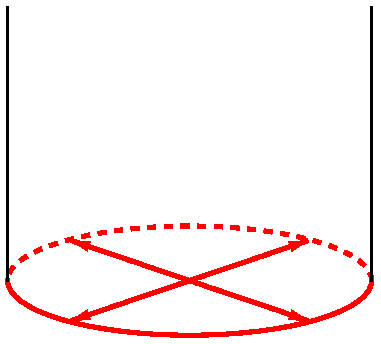
\includegraphics[width=.2\textwidth]{figures/crosscapstate.pdf}
\caption{The cross cap state $|\otimes\rangle$ is produced by the identification (\ref{crosscapbdry}) on the cylinder parameterized by $w\sim w + 2\pi$ with ${\rm Im}(w)\geq 0$.}\label{fig:crosscapstate}
\end{figure}


Analogously to the cylinder modular crossing equation (\ref{bccylcross}), the cross cap state is related to the Klein bottle partition function via
\ie\label{bccylcrosscap}
{\rm Tr}_{{\cal H}} \Omega b_0 c_0 e^{-{\pi t} (L_0+\wt L_0) } = {i\over t} \langle\langle \otimes | b_0 c_0 e^{-{\pi\over t} (L_0 + \wt L_0) } |\otimes\rangle,
\fe
where the factor $i/t$ on the RHS arises from the conformal translation of the $b,c$ ghost insertions. For the critical bosonic string theory, the LHS of (\ref{bccylcrosscap}) is evaluated by a partition sum over states with the same holomorphic and anti-holomorphic oscillator excitations,\footnote{Note that this is not the same as summing over worldsheet parity-invariant states, as the latter would correspond to the trace of $1+\Omega\over 2$ rather than $\Omega$.} giving
\ie
i V_X \int {d^{26} k_E \over (2\pi)^{26}} e^{-{\pi\over 2} \A' k_E^2 t} e^{2\pi n t} \prod_{n=1}^\infty (1-e^{-2\pi n t})^{-24} = i V_X (2\pi^2\A' t)^{-13} (\eta(it))^{-24}.
\fe
Comparison to the RHS of (\ref{bccylcrosscap}) with (\ref{crosscapexp}) then determines
\ie\label{notimes}
{\cal N}_{\otimes} = \pm e^{-{\pi i \over 4}} (2\pi^2\A')^{-{13\over 2}}.
\fe
To fix the sign of ${\cal N}_{\otimes}$ requires the consideration of the M\"obius strip partition function, with a D-brane boundary state on one side and the cross cap state on the other. It will turn out that the choice of the sign of (\ref{notimes}) gives rise to two different types of unoriented string theories with different spectra of D-branes. 

At the level of interacting string theory, however, the cross cap state (\ref{crosscapexp}) is a source of massless tadpole that signals the breakdown of string perturbation theory. It is possible to cancel the massless tadpole due to the cross cap state by that of space-filling D-branes. We will defer this analysis to section \ref{sec:typeitadpole} in the context of type I superstring theory.




\subsection{Type I string theory}
\label{sec:typei}

An unoriented version of superstring theory may be constructed starting from the type IIB string theory, which is defined with worldsheet parity-invariant GSO projection, and gauging the orientation-reversing diffeomorphism on the worldsheet. 

We begin by considering the Euclidean worldsheet cylinder in the superconformal gauge. The worldsheet parity $\Omega$ acts on the fields by (\ref{omegacyl}) together with
\ie\label{omegapsibc}
\Omega \psi^\mu(w) \Omega^{-1} = -i\hat\zeta \widetilde\psi^\mu(\bar w' = - w), ~~\Omega \C(w) \Omega^{-1} =  i\hat\zeta \widetilde\C(\bar w' = - w), ~~\Omega \B(w) \Omega^{-1} = i\hat\zeta \widetilde\B(\bar w' = - w), 
\fe
where $\hat\zeta =\pm 1$. The factors of $i$ and the relative signs on the RHS of (\ref{omegapsibc}) are necessary for the Lorentz current $\psi^\mu\psi^\nu$ as well as the BRST current to transform as worldsheet vectors. The analogous transformations of the anti-holomorphic fields are such that $\Omega$ obeys\footnote{One could alternatively consider $\Omega' \equiv  (-)^F \Omega$, which obeys $(\Omega')^2=1$ and acts the same way as $\Omega$ on GSO-projected states. Nonetheless, we will see below that $\Omega$ has a natural extension to the open string sector.}
\ie\label{omegaffp}
\Omega^2 = (-)^{F+\wt F},
\fe
where $(-)^F$ and $(-)^{\wt F}$ are the holomorphic and anti-holomorphic fermion parity respectively. By the state/operator map defined via the conformal transformation $z=e^{-i w}$, $\Omega$ acts on the fields on the $z$-plane according to (\ref{omegacylplane}) together with
\ie\label{omegapsibcz}
\Omega \psi^\mu(z) \Omega^{-1} = \hat\zeta \widetilde\psi^\mu(\bar z' = z), ~~\Omega \C(z) \Omega^{-1} =  \hat\zeta \widetilde\C(\bar z' = z), ~~\Omega \B(z) \Omega^{-1} = \hat\zeta \widetilde\B(\bar z' = z).
\fe
Acting on the space of states, $\Omega$ is defined to preserve $c\wt c$ in the (NS,NS) sector similarly to (\ref{omegakkdd}), and consequently leaves the graviton state invariant. Moreover, $\Omega$ exchanges the (NS,R) sector with the (R,NS) sector, and acts on the (R,R) sector ground state according to
\ie\label{rrgrdom}
\Omega \cdot c\widetilde c e^{-{\phi\over 2}} \Theta_\A e^{-{\widetilde\phi\over 2}}   \widetilde\Theta_{\B} = -  c\widetilde c e^{-{\widetilde\phi\over 2}} \Theta_\B e^{-{\phi\over 2}} \widetilde\Theta_{\A}.
\fe
The appearance of the minus sign on the RHS is due to the Grassmann-odd nature of the spacetime supersymmetry currents $j_\A= e^{-{\phi\over 2}} \Theta_\A$, $\wt j_\B = e^{-{\widetilde\phi\over 2}}   \widetilde\Theta_{\B}$, and would be necessary for the $\Omega$-projection to be compatible with spacetime supersymmetry.

The $\Omega$-invariant massless closed string states are represented by the vertex operators
\ie{}
& {\rm (NS,NS):} ~~~~ c\widetilde c e^{-\phi - \widetilde\phi} e_{(\mu\nu)} \psi^\mu \widetilde\psi^\nu e^{ik\cdot X},
\\
& {\rm (R,R):} ~~~~ c\widetilde c\, f^{[\A\B]} e^{-{\phi\over 2} } \Theta_\A e^{- {\widetilde\phi\over 2}} \widetilde\Theta_\B e^{ik\cdot X},
\\
& {\rm (NS,R)+(R,NS):} ~~~~ c\widetilde c\, u^{\mu\A}  \left( e^{-{\phi\over 2}} \Theta_\A e^{- \widetilde\phi} \widetilde\psi_\mu + e^{-\phi} \psi_\mu e^{- {\widetilde\phi\over 2}} \widetilde\Theta_\A  \right) e^{ik\cdot X},
\fe
where the polarization tensors $e_{\mu\nu}$, $f^{\A\B}$, $u^{\mu\A}$ obey the usual transversality constraints as in (\ref{kgammaspaeom}), (\ref{sustertrans}), and are further subject to the symmetry condition 
\ie
e_{\mu\nu} = e_{\nu\mu}, ~~~~f^{\A\B} = - f^{\B\A}.
\fe
Consequently, in the (NS,NS) sector there is no longer a $B$-field as the unoriented string cannot carry charge with respect to a 2-form gauge field. In the (R,R) sector, $f^{\A\B}$ must be a linear combination of $(\Gamma_{\mu\nu\rho})^{\A\B}$, and hence only the 3-form RR field strength is admissible. That is, the only RR field that survives $\Omega$-projection is the 2-form potential $C_2^{\rm RR}$. Completed with a single gravitino and a dilatino from the (NS,R)+(R,NS) sector, the massless unoriented closed string spectrum fits into the 10-dimensional ${\cal N}=(1,0)$ supergraviton multiplet.



Consistency of string perturbation theory requires the massless tadpole due to the cross cap to be canceled, potentially by that of space-filling D9-branes. To this end, we need to examine the worldsheet parity transformation of the open string states. Let us consider the worldsheet represented by a strip of width $\pi$, parameterized by complex coordinate $w$ with ${\rm Re}(w)\in [0,\pi]$. The worldsheet parity $\Omega$ exchanges the left and right ends of the open string, and acts on the fields on the strip as (\ref{omegacyl}) and (\ref{omegapsibc}) with an extra shift by $\pi$,
\ie\label{stripomegas}
& \Omega X^\mu(w,\bar w) \Omega^{-1}  = X^\mu(\pi-\bar w, \pi-w),~~~~ \Omega \psi^\mu(w) \Omega^{-1} = -i\hat\zeta \widetilde\psi^\mu(\bar w' = \pi - w),
\\
&  \Omega c(w) \Omega^{-1}  = - \wt c(\bar w' = \pi- w),~~~~  \Omega b(w) \Omega^{-1}  = \wt b(\bar w' =\pi - w),
\\
& \Omega \C(w) \Omega^{-1} =  i\hat\zeta \widetilde\C(\bar w' = \pi - w), ~~~~\Omega \B(w) \Omega^{-1} = i\hat\zeta \widetilde\B(\bar w' = \pi - w),
\fe
where $\hat\zeta=\pm 1$, and the transformations of the anti-holomorphic spinor fields are such that %\footnote{In contrast to the closed string sector as commented below (\ref{omegaffp}), in the open string sector we do not have the option of defining a conserved worldsheet parity operator that squares to 1 as opposed to $(-)^F$.}
\ie\label{omenft}
\Omega^2 = e^{2\pi i N_F},
\fe
where $N_F$ is the total {\it oscillator level} of the worldsheet spinor fields. Note that while $e^{2\pi i N_F}$ coincides with the fermion parity $(-)^F$ in the NS sector, they differ in the R sector. After mapping to the UHP via the conformal transformation $z=-e^{-iw}$, we can write the $\Omega$ transformations in the notation of the doubling trick (\ref{doublingtrickii}) for the D9-brane as
\ie\label{omegauhp}
& \Omega X_L^\mu(z) \Omega^{-1} = X_L^\mu(-z),~~~~ \Omega c (z) \Omega^{-1} = - c(-z),~~~~\Omega b(z) \Omega^{-1} = b(-z) ,
\\
& \Omega \psi^\mu(z)\Omega^{-1} = - i \hat\zeta \hat\eta \psi^\mu(-z),~~~~ \Omega \C(z) \Omega^{-1} = i \hat\zeta \hat\eta \C(-z),~~~~\Omega \B(z) \Omega^{-1} = i \hat\zeta \hat\eta \B(-z).
\fe
In the doubling trick representation, (\ref{omenft}) amounts to $2\pi$ rotation around the origin.

\begin{figure}[h!]
\centering
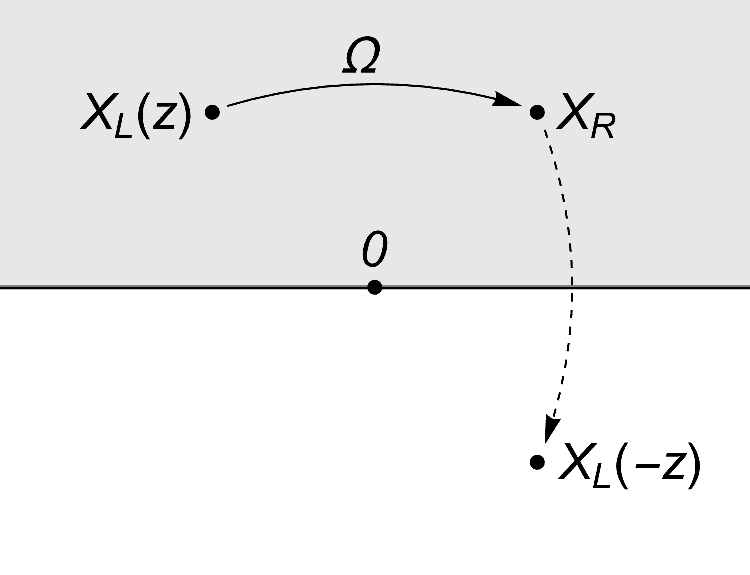
\includegraphics[width=.35\textwidth]{figures/doublingcrosscap.pdf}
\caption{The action of the worldsheet parity $\Omega$ represented through the doubling trick.}\label{fig:doublingcrosscap}
\end{figure}

%where $\hat\rho$ is a phase that takes the value $\hat\rho = \hat\zeta$ in the NS sector and $\hat\rho = \pm i \hat\zeta$ in the R sector.
In the presence of $n$ D9-branes, there is a further choice of $\Omega$ action on the Chan-Paton factor, as follows. Denote by $|ij\rangle$ the state that corresponds to the ``identity'' interface between the $i$-th and the $j$-th D9-brane, $i,j=1,\cdots, n$. Compatibility with the OPE as dictated by the algebra of $n\times n$ matrices ($U(n)$ Chan-Paton factor), up to an overall sign associated with the orientation of the boundary, requires 
\ie\label{omegacpfac}
\Omega |ij\rangle = \omega \C_{jj'} (\C^{-1})_{i'i} |j'i'\rangle
\fe
for some constant unitary matrix $\C \in U(n)$ and $\omega=\pm 1$. A more careful inspection of the string amplitudes shows that the consistent choice is $\omega = -1$. Furthermore, $\Omega^2|ij\rangle = |ij\rangle$, which requires $\C(\C^T)^{-1} = \pm \mathbb{I}_n$, i.e.
\ie
\C = \pm \C^T.
\fe
Up to a unitary change of basis under which $\C$ transforms by $\C\mapsto U \C U^T$ for some $U\in U(n)$, we can put
\ie\label{socp}
\C = \mathbb{I}_n
\fe 
in the case $\C^T=\C$, or 
\ie\label{spcp}
\C = i \begin{pmatrix} 0 & -\mathbb{I}_{n\over 2} \\  \mathbb{I}_{n\over 2}  & 0 \end{pmatrix}
\fe
in the case $\C^T= - \C$ (where $n$ must be even).


The $\Omega$-invariant massless NS open string states, in particular, are of the form
\ie\label{masslessomega}
ce^{-\phi} e_{\mu} \psi^\mu e^{ik\cdot X} \lambda_{ij} |ij\rangle,
\fe
where $\lambda_{ij}$ obeys
\ie\label{llttrans}
\C^{-1} \lambda \C = - \lambda^T.
\fe
Note that the minus sign on the RHS of (\ref{llttrans}) results from two factors of $i$ in the $\Omega$-transformation of $e^{-\phi}\simeq \delta(\C)$ and $\psi^\mu$ according to (\ref{omegauhp}),\footnote{The sign is consistent with the $\Omega$-transformation of the picture-raised version of the state.} whereas a minus sign from the $c$ ghost cancels against the sign $\omega=-1$ from (\ref{omegacpfac}). The $n\times n$ matrices $\lambda$ subject to the constraint (\ref{llttrans}) generate, with respect to commutators, the Lie algebra $so(n)$ in the case (\ref{socp}), and $sp(n)$ in the case (\ref{spcp}). Correspondingly, the open string states (\ref{masslessomega}) represent gauge bosons associated with $SO(n)$ or $Sp(n)$ gauge symmetry in the spacetime. 

We will see in the next section that the cancellation of massless closed string tadpoles is possible only in the presence of D9-branes with $SO(32)$ Chan-Paton factor. Miraculously, $SO(32)$ is also one of the two possible gauge groups (the other being $E_8\times E_8$, as seen in Chapter \ref{chap:hetstring}) that allows for the cancellation of gravitational and gauge anomalies of the ${\cal N}=1$ supergravity effective theory via the Green-Schwarz mechanism. The unoriented type IIB superstring with open strings that carry $SO(32)$ Chan-Paton is known as the {\it type I string theory}.



\subsection{Tadpole cancellation}
\label{sec:typeitadpole}

To construct the cross cap state of type I string theory, we consider as in section \ref{sec:crosscapbos} the semi-infinite Euclidean cylinder parameterized by complex coordinate $w$ with $w\sim w+2\pi$ and ${\rm Im}(w)\geq 0$, subject to the boundary condition (\ref{crosscapbdry}) together with
\ie{}
&  \lim_{{\rm Im}(w)\to 0} \big[ \psi^\mu(w) - \hat\zeta \wt\psi^\mu( \bar w+\pi ) \big] = 0,
\\
& \lim_{{\rm Im}(w)\to 0} \big[ \C(w) - \hat\zeta \wt \C(\bar w+\pi ) \big] = 0,~~~~\lim_{{\rm Im}(w)\to 0} \big[ \B(w) - \hat\zeta \wt \B(\bar w+\pi ) \big] = 0,
\fe
where the sign $\hat\zeta$ amounts to the choice of a spin structure associated with the cross cap.
The corresponding cross cap state 
\ie
|\otimes, \hat\zeta\rangle = |\otimes, \hat\zeta\rangle_{\rm NSNS} + |\otimes, \hat\zeta\rangle_{\rm RR}
\fe
satisfies
\ie\label{crosscapcondsup}
& (\A_n^\mu + (-)^n \wt \A_{-n}^\mu) |\otimes, \hat\zeta\rangle_\nu = (c_n + (-)^n \wt c_{-n}) |\otimes, \hat\zeta\rangle_\nu = (b_n - (-)^n \wt b_{-n}) |\otimes, \hat\zeta\rangle_\nu = 0,
\\
& (\psi_r^\mu - e^{ \pi i ({1\over 2}-r)} \hat\zeta \wt\psi_{-r}^\mu) |\otimes, \hat\zeta\rangle_\nu =  (\C_r^\mu + e^{ \pi i ({1\over 2}-r)} \hat\zeta \wt\C_{-r}^\mu) |\otimes, \hat\zeta\rangle_\nu =  (\B_r^\mu + e^{ \pi i ({1\over 2}-r)} \hat\zeta \wt\B_{-r}^\mu) |\otimes, \hat\zeta\rangle_\nu = 0,
\fe
where $r\in \mathbb{Z}+{1\over 2}$ for $\nu={\rm NSNS}$ and $r\in \mathbb{Z}$ for $\nu={\rm RR}$. The conditions (\ref{crosscapcondsup}) determine, up to normalization,
\ie\label{nscrosscap}
|\otimes, \hat\zeta\rangle_{\rm NSNS} &= i \hat\zeta {\cal N}_{\otimes,{\rm NSNS}}  \exp\bigg[ - \sum_{n=1}^\infty {(-)^n\over n} \A^\mu_{-n} \wt \A_{\mu,-n} + \sum_{n=1}^\infty (-)^n (c_{-n}\wt b_{-n} + \wt c_{-n} b_{-n}) 
\\
& + \hat\zeta \sum_{r\in \mathbb{Z}_{\geq 0} + {1\over 2}} e^{ \pi i ({1\over 2}-r)} \left( \psi^\mu_{-r} \wt\psi_{\mu, -r} + \C_{-r} \wt\B_{-r} - \wt \C_{-r} \B_{-r} \right)  \bigg] (c_0 + \wt c_0) |0; \downarrow,\downarrow\rangle \otimes |-1,-1\rangle,
\fe
and
\ie\label{rrcrosscap}
|\otimes, \hat\zeta\rangle_{\rm RR} &= {\cal N}_{\otimes,{\rm RR}} \exp\bigg[ - \sum_{n=1}^\infty {(-)^n\over n} \A^\mu_{-n} \wt \A_{\mu,-n} + \sum_{n=1}^\infty (-)^n (c_{-n}\wt b_{-n} + \wt c_{-n} b_{-n}) 
\\
& + i \hat\zeta \sum_{r=1}^\infty (-)^r \left( \psi^\mu_{-r} \wt\psi_{\mu,-r} + \C_{-r} \wt\B_{-r} - \wt \C_{-r} \B_{-r} \right)  \bigg] (c_0 + \wt c_0) |0; \downarrow,\downarrow\rangle \otimes |\Omega, \hat\zeta\rangle,
\fe
where $|\Omega, \hat\zeta\rangle$ are (R,R) ground states of the $(\psi,\B,\C;\wt\psi,\wt\B,\wt\C)$ system that satisfy (\ref{psibccond}) and are constructed as in (\ref{omagepa}) (with $\hat\eta$ replaced by $\hat\zeta$). Similarly to (\ref{dpavg}), the cross cap state averaged over spin structures
\ie
|\otimes\rangle = {1\over 2} \left( |\otimes,+\rangle + |\otimes,-\rangle \right)
\fe
satisfies the type IIB GSO projection.

The normalization factors ${\cal N}_{\otimes,{\rm NSNS}}$ and ${\cal N}_{\otimes,{\rm RR}}$ can be fixed by the relation between the cross cap state and the Klein bottle partition function with various spin structure assignments and suitable ghost insertions, generalizing (\ref{bccylcrosscap}) and similarly to (\ref{dpabr}),
\ie\label{kleincrosssup}
& {\rm Tr}_{{\cal H}_{\rm NSNS}} \Omega  b_0 c_0 e^{-{\pi t} (L_0+\wt L_0) } = {-i\over t} \langle\langle \otimes,- |_{\rm NSNS}  e^{-{\pi\over t} (L_0 + \wt L_0) }b_0 c_0 |\otimes,+\rangle_{\rm NSNS},
\\
& {\rm Tr}_{{\cal H}_{\rm RR}} \Omega  b_0 c_0 e^{-{\pi t} (L_0+\wt L_0) } = {-i\over t} \langle\langle \otimes,+ |_{\rm NSNS}  e^{-{\pi\over t} (L_0 + \wt L_0) }b_0 c_0 |\otimes,+\rangle_{\rm NSNS},
\\
& {\rm Tr}_{{\cal H}_{\rm NSNS}}(-)^{F} \Omega  b_0 c_0 e^{-{\pi t} (L_0+\wt L_0) } = {-i\over t} \langle\langle \otimes,- |_{\rm RR}'  e^{-{\pi\over t} (L_0 + \wt L_0) }b_0 c_0 |\otimes,+\rangle_{\rm RR},
\\
& {\rm Tr}_{{\cal H}_{\rm RR}} (-)^{F}\Omega  b_0 c_0 \delta(\B_0) \delta(\C_0) e^{-{\pi t} (L_0+\wt L_0) } = {-i\over t} \langle\langle \otimes,+ |_{\rm RR}'  e^{-{\pi\over t} (L_0 + \wt L_0) }b_0 c_0 \delta(\C_0)\delta(\B_0) |\otimes,+\rangle_{\rm RR}.
\fe
Here the RR cross cap states $|\otimes, \hat\eta\rangle_{\rm RR}$ and $|\otimes, \hat\eta\rangle_{\rm RR}$ are constructed from the ground states $|\Omega, \hat\zeta\rangle$ and $|\Omega, \hat\zeta\rangle'$ defined in (\ref{omagepa}) in the $p=9$ case, and carry picture number $(-{3\over 2},-{1\over 2})$ and $(-{1\over 2},-{3\over 2})$ respectively. Note that the trace with $\Omega$ insertion, as appearing in the first two lines of (\ref{kleincrosssup}), is calculated by the path integral on the Klein bottle parameterized by the spatial coordinate $\sigma\sim \sigma + 2\pi$ and Euclidean time coordinate $\tau$, subject to the fermion periodicity condition
\ie{}
& \psi^\mu(\sigma,\tau) = i\hat\zeta \wt\psi^\mu(-\sigma,\tau+\pi t) = -\psi^\mu(\sigma, \tau+2\pi t),
\\
& \wt\psi^\mu(\sigma,\tau) = - i\hat\zeta \psi^\mu(-\sigma,\tau+\pi t) = -\wt \psi^\mu(\sigma, \tau+2\pi t),
\fe
and similarly for $\B,\C$. The anti-periodicity of both $\psi^\mu$ and $\wt\psi^\mu$ under $\tau \mapsto \tau +2\pi t$ indicates the propagation of the (NS,NS) component of the cross cap state in the cross channel. Likewise, the trace with $(-)^F\Omega$ insertion in the last two lines of (\ref{kleincrosssup}) is calculated by the path integral with $\psi^\mu, \wt\psi^\mu$ periodic under $\tau \mapsto \tau +2\pi t$, and corresponds to the propagation of the (R,R) component of the cross cap state.

The LHS of the first line of (\ref{kleincrosssup}) is explicitly evaluated as
\ie\label{ccparsm}
 {\rm Tr}_{{\cal H}_{\rm NSNS}} \Omega b_0 c_0 e^{-{\pi t} (L_0+\wt L_0) }
&= {i V_X} (2\pi^2\A' t)^{-5} (\eta(it))^{-8} \left[ {\theta_3(0|it)\over \eta(it)} \right]^4 
\\
&= {1\over t} {i V_X} (2\pi^2\A' )^{-5} (\eta(i/t))^{-8}  \left[ {\theta_3(0|i/t)\over \eta(i/t)} \right]^4 ,
\fe
where %the minus sign for the RR contribution follows the minus sign on the RHS of (\ref{rrgrdom}), and 
a modular transformation is performed to arrive at the last line. Comparison with the RHS of the first line of (\ref{kleincrosssup}) then determines
\ie\label{ncrosscapns}
{\cal N}_{\otimes, {\rm NSNS}} = \pm e^{{\pi i\over 4}} 2^{5\over 2} (2\pi \sqrt{\A'})^{-5}.
\fe
A calculation similar to (\ref{ccparsm}) with $(-)^F$ insertion determines ${\cal N}_{\otimes,{\rm RR}}$ to be of the same value as ${\cal N}_{\otimes, {\rm NSNS}}$, up to a sign. To fix the signs, we must compare the cross cap state with the D-brane boundary states, as follows.

Consider the following partition function on the strip twisted by $\Omega$, 
\ie\label{mobiuscross}
{\rm Tr}_{{\cal H}^o_{\rm NS}} {1+(-)^F\over 2} \Omega (-)^{N_{bc}+N_{\B\C}} b_0 c_0 e^{- \pi t L_0} = {-i\over t}\langle\langle B |_{\rm NSNS} e^{-{\pi\over 2t} (L_0 + \widetilde L_0 )}b_0c_0 |\otimes\rangle_{\rm NSNS} ,
\fe
which may also be interpreted as the partition function on the M\"obius strip averaged between two (out of four possible) choices of spin structures. On the LHS, the trace is taken over the space ${\cal H}^o_{\rm NS}$ of NS sector states on the strip of width $\pi$, subject to boundary condition $B$ on both sides, with $\Omega$ acting according to (\ref{stripomegas}). In the path integration representation, the fermion fields are subject to periodicity condition\footnote{Note that the analogous periodicity condition in the path integral that computes the trace over ${\cal H}_{\rm R}^o$ is $\psi^\mu(\sigma,\tau) = + \psi^\mu(\sigma,\tau+2\pi t)$, by virtue of (\ref{omenft}).}
\ie\label{hatrhopsi}
\psi^\mu(\sigma,\tau) = \pm i\hat\zeta \wt\psi^\mu(\pi-\sigma,\tau+\pi t) %= (\pm i\hat\zeta)^2 \psi^\mu(\sigma,\tau+2\pi t) 
= - \psi^\mu(\sigma,\tau+2\pi t),
\fe
where the two signs after the first equality corresponds to the trace without and with $(-)^F$ insertion. Therefore, %As $\hat\rho^2=1$ 
%in the NS sector, %it follows from (\ref{hatrhopsi}) that 
$\psi^\mu$ is anti-periodic under $\tau\mapsto \tau + 2\pi t$. Up to a conformal transformation that involves rescaling by $1/t$ and rotation by $90^\circ$, the twisted partition function may be equivalently viewed as a matrix element of the Euclidean propagator (over Euclidean time $\pi/(2 t)$) between the GSO-projected boundary state and the cross cap state, as given by the RHS of (\ref{mobiuscross}).

Using (\ref{omegauhp}) and (\ref{omegacpfac}), we can evaluate the LHS of (\ref{mobiuscross}) as
\ie\label{intcpnvx}
&  \pm n  { i V_X} (4\pi^2 \A' t)^{-5} e^{\pi t} \prod_{k=1}^\infty \left(1-(-)^k e^{-{k \pi t}}\right)^{-8} 
\\
& \times {-i \hat\zeta\hat\eta\over 2}\left[ \prod_{m=0}^\infty \left(1 - i \hat\zeta\hat\eta (-)^m e^{-(m+{1\over 2}){\pi t}}\right)^8 - \prod_{m=0}^\infty \left(1 + i \hat\zeta\hat\eta (-)^m e^{-(m+{1\over 2}) {\pi t} } \right)^8 \right] 
\\
&=  \mp n  { i V_X} (4\pi^2 \A' t)^{-5} \left(\eta(\tfrac{it+1}{ 2})\right)^{-8} \left\{ \left[{\theta_3(0|\tfrac{it+1}{2})\over \eta(\tfrac{it+1}{2})}\right]^4 - \left[{\theta_4(0|\tfrac{it+1}{2})\over \eta(\tfrac{it+1}{2})}\right]^4 \right\},
\fe
where the factor $\pm n$ comes from the trace of $\Omega$ over the $SO(n)$ or $Sp(n)$ Chan-Paton factor. Using the $PSL(2,\mathbb{Z})$ modular transformation property of the $\eta$-function and the Jacobi theta functions under
\ie
\tau \mapsto \tau' = {\tau-1\over 2\tau - 1},
\fe
which takes $\tau = {it+1\over 2}$ to $\tau' = {it^{-1}+1\over 2}$,
we can rewrite (\ref{intcpnvx}) as
\ie{}
& \mp {n\over t}  { i V_X} (4\pi^2 \A')^{-5} \left(\eta(\tfrac{it^{-1}+1}{ 2})\right)^{-8} \left\{ \left[{\theta_3(0|\tfrac{it^{-1}+1}{2})\over \eta(\tfrac{it^{-1}+1}{2})}\right]^4 - \left[{\theta_4(0|\tfrac{it^{-1}+1}{2})\over \eta(\tfrac{it^{-1}+1}{2})}\right]^4 \right\}
\\
&=  \pm {n\over t}  { i V_X} (4\pi^2 \A')^{-5} e^{\pi/ t} \prod_{k=1}^\infty \left(1-(-)^k e^{-{k \pi/ t}}\right)^{-8} 
\\
& ~~~ \times {i \over 2}\left[ \prod_{m=0}^\infty \left(1 + i  (-)^m e^{-(m+{1\over 2}){\pi/ t}}\right)^8 - \prod_{m=0}^\infty \left(1 - i  (-)^m e^{-(m+{1\over 2}) {\pi /t} } \right)^8 \right] .
\fe
This precisely agrees with the RHS of (\ref{mobiuscross}) evaluated using the boundary state (\ref{nsdryst}) for $n$ D9-branes and the cross cap state (\ref{nscrosscap}), provided that the choice of sign in (\ref{ncrosscapns}) is $-$ in the $SO(n)$ case and $+$ in the $Sp(n)$ case, or equivalently
\ie
{\cal N}_{\otimes, {\rm NSNS}} = \left\{ \begin{array}{l} - 2^5 {\cal N}_{{\rm D}9,{\rm NSNS}},~~~~SO \\  + 2^5 {\cal N}_{{\rm D}9,{\rm NSNS}},~~~~Sp \end{array}  \right.
\fe
A similar calculation of the M\"obius strip partition function with Ramond type spin structure assignment shows that ${\cal N}_{\otimes, {\rm RR}}=\mp 2^5 {\cal N}_{{\rm D}9,{\rm RR}}$ in the $SO/Sp$ case as well.\footnote{Note that in this computation, the trace over Ramond sector states on the strip comes with an overall minus sign due to the fermionic spacetime statistics.} One can then easily verify that the total massless tadpole in the presence of $n$ D9-branes, which is proportional to the $L_0 = \wt L_0=0$ component of the cross cap plus boundary state
\ie
|\otimes\rangle + n |{\rm D}9\rangle, 
\fe
vanishes in both the (NS,NS) and (R,R) sectors if and only if the Chan-Paton factor is of the $SO$ type with $n=32$, as promised. The cross cap state may be equivalently viewed as the closed string field sourced by a spacetime object that reverses the orientation of the string, known as the {\it orientifold}.



\subsection{Type I string amplitudes}

The perturbative type I string S-matrix can be formulated by a straightforward extension of the open+closed superstring perturbation theory of section \ref{sec:openclosedpertsuper}. Starting with the worldsheet theory of type IIB superstring in the superconformal gauge, we will allow for both oriented and unoriented surfaces, with boundaries subject to the boundary condition that correspond to 32 D9-branes. Generalizing (\ref{openclosedsupamppco}), the open+closed amplitude at Euler characteristic $\chi$ can be expressed as
\ie\label{openclosedtypeiamppco}
{\cal A}_{\chi}\left[\{V_i^c\}_{1\leq i\leq n}, \{V_j^o\}_{1\leq j\leq m}\right] = \mathfrak{N}_{\chi, n,m}  \int_{\cal S} \wt \Omega,
\fe
where ${\cal S}$ is a suitable contour in the fiber bundle $\pi: {\cal Y}_{\chi;n,m} \to {\cal M}_{\chi;n,m}$, whose fiber is parameterized by the positions of the PCOs and the choice of the spin structure, and whose base is the moduli space of all oriented and unoriented Riemann surfaces $\Sigma$ of Euler characteristic $\chi$ with $n$ bulk punctures and $m$ boundary punctures. In particular, the projection $\pi({\cal S})$ covers the moduli space once for each spin structure. The differential form $\wt\Omega$ is defined through the worldsheet correlator as in (\ref{wtompcoop}). The Euler characteristic $\chi$ is related to the genus $h$, the number of boundaries $b$, and the number of cross caps $c$ by (\ref{chihbc}). Similarly to section \ref{sec:unitarysuper}, the normalization factor $\mathfrak{N}_{\chi, n,m}$ is determined by unitarity to be
\ie\label{normunoriented}
\mathfrak{N}_{\chi, n,m} =  2^{{3\over 2}\chi-3 + {m\over 4}} e^{\left( -{3\over 2}\chi + n +{3\over 4}m\right){\pi i \over 2}}.
\fe
Note that for an oriented surface of genus $h$ with $b$ boundaries, $\mathfrak{N}_{\chi, n,m}$ is equal to (\ref{normopensup}) multiplied by the extra factor $2^{-h - {b\over 2} + {m\over 4}}$. In particular, the normalization is such that the amplitude factorizes through on-shell intermediate states that are invariant under worldsheet parity $\Omega$, and the inclusion of the factor $2^{m\over 4}$ in (\ref{normunoriented}) ensures that the open string propagator (loosely speaking given by the inverse of the disc 2-point amplitude) is canonically normalized.

The type I string field theory can be constructed similarly to the open+closed superstring field theory of section \ref{sec:ocsftsup}, now with open and closed string fields defined to be $\Omega$-invariant and including string vertices that contain cross caps. For details see Faroogh Moosavian, Sen, Verma, JHEP \textbf{01} (2020), 183 \cite{FarooghMoosavian:2019yke}.




\subsubsection{Vacuum amplitude}

Let us illustrate the role of the normalization factor (\ref{normunoriented}) with the vacuum amplitude at $\chi=0$, which amounts to the closed and open 1-loop correction to the vacuum energy density. There are four distinct topologies that contribute: the torus, the Klein bottle, the cylinder, and the M\"obius strip.

The torus vacuum amplitude of type I string theory is formally ${1\over 2}$ times that of type IIB string theory,
\ie\label{torustypei}
{\cal A}_{ T^2} &= 2^{-3} \sum_{\epsilon_L, \epsilon_R} \int_{\cal F} {id\tau\wedge d\bar\tau\over 4\tau_2}  \left\langle \wt b b c\wt c \right\rangle_{T^2(\tau), \epsilon_L,\epsilon_R}
\\
& = {1\over 2} \int_{-{1\over 2}}^{1\over 2} d\tau_1 \int_{\tau_2>0,\; |\tau|>1} {d\tau_2\over 2\tau_2} {\rm STr}_{\cal H} {1+(-)^F\over 2} {1+(-)^{\wt F}\over 2} (-)^{N_{bc} + N_{\B\C} } \wt b_0 b_0 c_0 \wt c_0 e^{2\pi i \tau L_0 - 2\pi i \bar\tau \wt L_0},
\fe
where ${\rm STr}$ stands for the trace over the space of states ${\cal H}$ of the worldsheet SCFT on the circle, with an extra minus sign assigned to the (NS,R) and (R,NS) sectors (due to fermionic spacetime statistics), and the trace in Ramond sector is understood to be regularized as in (\ref{twistchareg}), (\ref{parttwsithir}).

The Klein bottle ($K^2$) vacuum amplitude can be expressed in terms of the trace over ${\cal H}$ with the insertion of the worldsheet parity operator $\Omega$, integrated over the moduli space parameterized by $t>0$ as
\ie\label{kleintypei}
{\cal A}_{ K^2} = {1\over 2} \int_0^\infty {d t\over 2t} {\rm Tr} {1+(-)^F\over 2} {1+(-)^{\wt F}\over 2} \Omega  b_0 c_0 e^{-2\pi t ( L_0 + \wt L_0) }.
\fe
Note that the trace only receives contribution from the (NS,NS) and (R,R) sectors. From the string field theory standpoint, the combined contribution to the torus amplitude (\ref{torustypei}) from sufficiently large $\tau_2$ and to the Klein bottle amplitude (\ref{kleintypei}) from sufficiently large $t$ are reproduced by the 1-loop vacuum diagram of the $\Omega$-invariant closed string fields in the Siegel gauge (whose propagator comes with the projector ${1+\Omega\over 2} \delta_{L_0, \wt L_0}$).

Similarly, the cylinder ($C^2$) and the M\"obius strip ($M^2$) vacuum amplitudes combine into\footnote{In the notation of (\ref{openclosedtypeiamppco}), there are four spin structures associated with the two boundaries of the cylinder, or one boundary and one cross cap of the M\"obius strip, that combines with the normalization factor $2^{-3}$ to give (\ref{cylmobtypei}).}
\ie\label{cylmobtypei}
{\cal A}_{ C^2} + {\cal A}_{ M^2} =
\int_0^\infty {dt\over t} \, {\rm STr}_{{\cal H}^o} {1+(-)^F\over 2} {1+\Omega\over 2} (-)^{N_{bc}+N_{\B\C}} b_0 c_0 e^{-2\pi t L_0},
\fe
where ${\cal H}^o$ is the space of states on the strip subject to the boundary condition of 32 D9-branes, and ${\rm STr}_{{\cal H}^o} \equiv {\rm Tr}_{{\cal H}^o_{\rm NS}} - {\rm Tr}_{{\cal H}^o_{\rm R}}$. (\ref{cylmobtypei}) can also be interpreted in terms of the 1-loop vacuum diagram of the $\Omega$-invariant open string field in the Siegel gauge.

A priori, (\ref{kleintypei}) and (\ref{cylmobtypei}) contain potentially divergent contributions from the $t\to 0$ limit of their respectively moduli spaces, which may be interpreted in the closed string channel as due to the exchange of massless closed string modes sourced by the D9-brane and the orientifold. The cancellation of these divergences, separately with respect to each closed string mode, is ensured by the tadpole cancellation condition analyzed in section \ref{sec:typeitadpole}. In fact, the full vacuum amplitude also vanishes, as a consequence of the spacetime supersymmetry of type I string theory.






\subsubsection{Spacetime effective theory}

The spacetime massless effective theory of type I string theory consists of the metric $G_{\mu\nu}$, dilaton $\Phi$, the RR 2-form $(C_2)_{\mu\nu}$, together with the gravitino and dilatino from the closed string sector, and the $SO(32)$ gauge field $A_\mu$ as well as the gaugino from the open string sector, governed by an effective action that is similar to the bulk-brane effective action considered in section \ref{sec:dbrangravex} (with a space-filling brane), of the form
\ie\label{typeiseff}
S_{\rm I} =  \int d^{10} x \sqrt{-\det G} \left\{ e^{-2\Phi} \left[ {1\over 2\kappa^2}  R(G) + \cdots\right] + e^{-\Phi} \left[ - {1\over 4 g_{\rm YM}^2}  {\rm tr} (F_{\mu\nu} F^{\mu\nu}) + \cdots \right]  \right\}.
\fe
The dilaton dependence in the terms proportional to $e^{-2\Phi}$ and $e^{-\Phi}$ are dictated by the sphere and disc topologies respectively. The gravitational coupling $\kappa$ and the gauge coupling $g_{\rm YM}$ can be determined by comparison to the 3-point sphere amplitude of closed strings and the 3-point disc amplitude of open strings to be
\ie\label{kappagymtypei}
\kappa = {\pi\over 2} g_s, ~~~~ g_{\rm YM}^2 = \sqrt{2}{g_o^2\over 8\A'} = 2^{7\over 2} \pi^{9\over 2} \A' g_s.
\fe
Note that while the relation between $\kappa$ and $g_s$ is as in (\ref{typeiigskap}), the relation between $g_{\rm YM}$ and $g_o$ differs from (\ref{gymgobos}) by a factor of $2^{1\over 4}$ due to the different normalization factor (\ref{normunoriented}) appearing in the disc amplitude.\footnote{While our convention for the open string coupling $g_o$ differs from that of Polchinski, {\it String theory. Vol. 2}, the relation between $\kappa$ and $g_{\rm YM}$ in (\ref{kappagymtypei}) is in agreement with Polchinski's (13.3.31).} 

As is generally the case for the bulk-brane effective action, (\ref{typeiseff}) does not admit a classical limit with dynamical bulk fields, as the tree-level closed string exchange diagram can also be viewed as a 1-loop open string diagram. Rather, (\ref{typeiseff})  should be viewed as a quantum effective action in the Wilsonian or 1PI sense. At leading orders in the derivative expansion, (\ref{typeiseff}) is constrained by spacetime supersymmetry to be that of type I supergravity with $SO(32)$ gauge group. We have already encountered the latter in the context of heterotic string theory in section \ref{sec:heteffth}. However, unlike in the heterotic string theory where the spacetime anti-symmetric 2-form potential arises from the (NS,NS) $B$-field, in type I string theory it comes from the (R,R) sector. 

Similarly to the Chern-Simons coupling on the D$p$-brane analyzed in sections \ref{sec:disccs} and \ref{sec:csdpcoup}, the disc amplitudes give rise to Chern-Simons type couplings between the RR 2-form $C_2$ and its electric-magnetic dual $C_6$ with the $SO(32)$ gauge field $A_\mu$ in the effective action of the form
\ie\label{csstypei}
{1\over \sqrt{2}}\mu_9 \int  \left[ {(2\pi\A')^2 \over 2} C_6\wedge  {\rm tr}_{\rm v} (F_2)^2 + {(2\pi \A')^4\over 4!} C_2\wedge {\rm tr}_{\rm v} (F_2)^4 \right],
\fe
where $\mu_9$ is given as in (\ref{mutprel}), (\ref{tpkapsup}). The first term in (\ref{csstypei}) reproduces the 2-derivative Chern-Simons coupling of type I supergravity due to the anomalous gauge transformation of the 2-form potential, whereas the second term in (\ref{csstypei}) is a part of the Green-Schwarz term (\ref{gsmech}) that is required for the cancellation of spacetime gauge anomaly.







\subsection{D-branes in type I string theory}
\label{sec:typeibrane}

\subsubsection{BPS D1 and D5-branes}
\label{sec:typeibranedone}

To describe D$p$-branes of type I string theory, we begin by analyzing the worldsheet parity transformation of open strings on a BPS D$p$-brane in type IIB string theory, for odd $p<9$. On the strip subject to the boundary condition of a D$p$-brane located at $X^{p+1} = \cdots = X^9=0$, the $\Omega$-transformation on the bulk fields (\ref{stripomegas}) remain valid. After applying the doubling trick (\ref{doublingtrick}), (\ref{doublingtrickii}), the $\Omega$-transformations of $X_L^\mu$ and $\psi^\mu$ read, in place of (\ref{omegauhp}),
\ie\label{omegauhpacss}
& \Omega X_L^\mu(z) \Omega^{-1} = X_L^\mu(-z),~~~~  \Omega \psi^\mu(z)\Omega^{-1} = - i \hat\zeta \hat\eta \psi^\mu(-z) ,~~~~ \mu=0,\cdots, p,
\\
& \Omega X_L^i(z) \Omega^{-1} = -X_L^i(-z),~~~~  \Omega \psi^i(z)\Omega^{-1} =  i \hat\zeta \hat\eta \psi^i(-z) ,~~~~ i=p+1,\cdots, 9.
\fe 
We also need to keep track of the $\Omega$-transformation of the spin fields on the strip, in particular of the spacetime supersymmetry current $j_\A = e^{-{\phi\over 2}} \Theta_\A$, which in the notation of the doubling trick (\ref{doublingtrickii}) takes the form
\ie\label{omegajj}
\Omega j_\A (z) \Omega^{-1} = - \left((\B^{p+1}\cdots\B^9)^{-1} j\right)_\A(-z).
\fe
Compatibility of (\ref{omegajj}) with $\Omega^2=1$ requires $9-p \equiv 0$ mod 4. Therefore, it is possible to gauge the worldsheet parity in the presence of a BPS D$p$-brane for $p=1$ or $5$, which defines the D1 or D5-brane in type I string theory.

It remains to determine the $\Omega$ action on the Chan-Paton factor of D1 and D5-branes. Given $n$ coinciding D1-branes, let $|ij\rangle_{{\rm D}1}$ be the state that corresponds to the identity boundary operator at the interface between the boundary conditions that correspond to the $i$-th and $j$-th D1-brane. By the same consideration of (\ref{omegacpfac}), $\Omega$ acts by
\ie\label{omegadone}
\Omega |ij\rangle_{{\rm D}1} = - (\C_{{\rm D}1})_{jj'} (\C_{{\rm D}1}^{-1})_{i'i} |j'i'\rangle_{{\rm D}1},
\fe
where $\C_{{\rm D}1}$ is a priori an $n\times n$ unitary matrix that is either symmetric or anti-symmetric. The correct choice can be determined by computing the M\"obius strip partition function, similarly to (\ref{mobiuscross}) except that the boundary state $|B\rangle$ is now taken to be that of the $n$ D1-branes (as in type IIB string theory), whereas the cross cap state $|\otimes\rangle$ is the same as the one determined in section \ref{sec:typeitadpole}. In the end one finds that $\C_{{\rm D}1}$ must be symmetric, and thus can be taken to be $\C_{{\rm D}1}=\mathbb{I}_n$.

In the case of single D1-brane, the $\Omega$-invariant massless NS open string states are 
\ie
c e^{-\phi} \psi^i e^{ik_\parallel\cdot X} |11\rangle_{\rm D1}, ~~~i=2,\cdots, 9,
\fe
corresponding to the transverse collective coordinates, where $k_\parallel$ is a lightlike momentum along the 1+1 dimensional world volume. Note that crucially, $\Omega$ acts on $\psi^{i=2,\cdots 9}$ (subject to Dirichlet boundary condition) with the opposite sign as on $\psi^{0,1}$ (subject to Neumann boundary condition). The $\Omega$-invariant massless Ramond open string states are
\ie\label{donetypeiramond}
c u^\A j_\A e^{ik_\parallel\cdot X} |11\rangle_{{\rm D}1},
\fe
where the polarization spinor $u^\A$ obeys
\ie\label{uuconda}
-u = u  \B^2 \cdots \B^9~~~{\rm and}~~~ k_\parallel^\mu \Gamma_\mu u = 0.
\fe
The first condition of (\ref{uuconda}), which follows from $\Omega$-invariance, is equivalent to $\Gamma^{01}u = -u$. While the momentum $k_\parallel$ obeys the lightlike mass-shell condition $k_\parallel^0 = \pm k_\parallel^1$, the second condition of (\ref{uuconda}) further requires $k_\parallel^0 = -k_\parallel^1$. Therefore, (\ref{donetypeiramond}) describes 8 {\it negative-momentum} massless fermions on the D1-brane, which transform in a spinor representation with respect to the $SO(8)$ that rotates the transverse directions. Indeed, the D1-brane preserves half of the 16 supersymmetries of type I string theory, whereas the massless states (\ref{donetypeiramond}) can be interpreted as Goldstinos associated with the 8 broken supersymmetries.

The D1-brane in type I string theory also supports open strings with one end on the D1-brane and the other end on the space-filling D9-branes. As $\Omega$ exchanges the left and right ends of the open string, it exchanges D1-D9 and D9-D1 string states in the type IIB theory, and therefore the $\Omega$-invariant states can be identified with those of the D1-D9 string only. The latter is a special case of the D$p$-D$p'$ system analyzed in section \ref{sec:intbrane}, where the lowest level NS and R open string states involve the matter vertex operators (\ref{nsndbdry}) and (\ref{rndbdry}) respectively. It follows from (\ref{mkdnd}) (with $d_{\rm ND}=8$) that there are no massless D1-D9 string states in the NS sector (as the lowest NS string state has $m^2 = {1\over 2\A'}$). The R sector, on the other hand, contains massless states of the form
\ie\label{sigmathetdnin}
c\Sigma  e^{-{\phi\over 2}} \Theta_+ e^{ik_\parallel \cdot X} |1,j \rangle_{{\rm D1},{\rm D9}},
\fe
where $\Sigma$ is a weight ${1\over 2}$ operator built out of the product of 8 $\mathbb{Z}_2$ twist fields of chiral bosons (see the discussions around (\ref{chiralbostwisexp})), and $\Theta_+$ is the weight ${1\over 8}$ spin field of the $\psi^0, \psi^1$ system, whose chirality is selected by the GSO projection. The state $|1,j\rangle_{{\rm D1},{\rm D9}}$ accounts for the Chan-Paton factor associated with the D1-brane and 32 D9-branes (the latter labeled by $j=1,\cdots,32$). The BRST closure condition further restricts the lightlike momentum $k_\parallel$ to be such that $k_\parallel^0 = k_\parallel^1$.\footnote{This is compatible with the invariance of the states (\ref{sigmathetdnin}) with respect to the chiral supersymmetries preserved by the D1-brane.} Therefore, (\ref{sigmathetdnin}) describes 32 massless fermions that propagate with {\it positive momentum} along the D1-brane, and transform in the vector representation of the $SO(32)$ gauge group of type I string theory.

Next we turn to the D5-branes. The analog of (\ref{omegadone}) on $n$ coincident D5-branes of type IIB string theory is
\ie\label{omegadfive}
\Omega |ij\rangle_{{\rm D}5} = - (\C_{{\rm D}5})_{jj'} (\C_{{\rm D}5}^{-1})_{i'i} |j'i'\rangle_{{\rm D}5},
\fe
where the unitary matrix $\C_{{\rm D}5}$ turns out to be {\it anti-symmetric}. To see this from the M\"obius strip partition function would require considering the contributions to (\ref{mobiuscross}) from the two spin structures separately, as they sum up to zero in the case of the D5-brane boundary condition. An easier way to determine the symmetry property of $\C_{{\rm D}5}$ is to consider the $\Omega$ action on the Chan-Paton factor of the D5-D9 open string,
\ie\label{omegafivenine}
\Omega |ij\rangle_{{\rm D5}, {\rm D9}} = - (\C_{{\rm D}9})_{jj'} (\C_{{\rm D}5}^{-1})_{i'i} |j'i'\rangle_{{\rm D9,D5}},
\fe
where $\C_{\rm D9}$ is symmetric (and may be set to the identity matrix). The lowest D5-D9 string states involve matter vertex operator of the form (\ref{nsndbdry}) and (\ref{rndbdry}). In the NS sector, for instance, the oscillator ground state is built out of chiral spin fields in the system of $d_{\rm ND}=4$ fermions, which must transform with phase $\pm i$ under $\Omega$ by compatibility with the OPE. In order to maintain $\Omega^2=1$ on the physical D5-D9 string states, the transformation on the Chan-Paton factor (\ref{omegafivenine}) must square to $-1$, and thus we conclude that $\C_{\rm D5}$ is anti-symmetric. 

Consequently, the D5-brane system in type I string theory exists only for even $n$, in which case the D5-D5 open string states carry $Sp(n)$ Chan-Paton factor. In the simplest $n=2$ case, we may take $\C_{\rm D5} = \sigma_2$ as in (\ref{spcp}). With the D5-brane extended in $X^0,\cdots, X^5$ directions, the massless NS open string states are
\ie\label{sigmalama}
c e^{-\phi} e_\mu\psi^\mu e^{ik_\parallel\cdot X} \lambda_{ij} |ij\rangle_{\rm D5}, ~~~~ c e^{-\phi} \psi^{6,7,8,9} e^{ik_\parallel\cdot X} \lambda_{ij}' |ij\rangle_{\rm D5},
\fe
where $e_\mu$ is a polarization vector along the world volume direction that obeys $e\cdot k_\parallel = 0$, and $\lambda, \lambda'$ are constrained by $\Omega$-invariance to obey
\ie\label{sigmalamb}
\sigma_2\lambda\sigma_2 = -\lambda^T,~~~~\sigma_2\lambda'\sigma_2 = (\lambda')^T.
\fe
It follows that $\lambda$ is a linear combination of the Pauli matrices $\sigma_{1,2,3}$, giving rise to $Sp(2)\simeq SU(2)$ gauge bosons, whereas $\lambda'$ is proportional to $\mathbb{I}_2$, corresponding to (a single set of) transverse collective coordinates. Therefore, the $n=2$ D5-brane system, upon $\Omega$-projection, describe a {\it single} D5-brane of type I string theory, with $SU(2)$ gauge fields on its world volume. The latter combine with the massless R sector D5-D5 string states to form a gauge multiplet with respect to the 6-dimensional ${\cal N}=(1,0)$ supersymmetry.

The D5-D9 open strings give rise to additionally 2 sets of massless {\it complex} scalars that carry $({\bf 2},{\bf 32})$ Chan-Paton factor with respect to the $SU(2)\times SO(32)$ gauge group from the NS sector, and an equal number of massless fermions from the R sector. Altogether, the massless D5-D9 string states form a 6-dimensional hypermultiplet in the $({\bf 2}, {\bf 32})$ representation.




%\ie\label{trnswomf}
%&{\rm Tr}_{{\cal H}^o_{\rm NS}} \Omega (-)^{N_{bc}+N_{\B\C}} b_0 c_0 e^{- \pi t L_0} 
%\\
%&=   \pm n  { i V_{\rm D5}} (4\pi^2 \A' t)^{-3} e^{\pi t} \prod_{k=1}^\infty \left(1-(-)^k e^{-{k \pi t}}\right)^{-4} \left(1+ (-)^k e^{-{k \pi t}}\right)^{-4} 
%\\
%& ~~~ \times (-i \hat\rho\hat\eta)  \prod_{m=0}^\infty \left(1 - i \hat\rho\hat\eta (-)^m e^{-(m+{1\over 2}){\pi t}}\right)^4  \prod_{m=0}^\infty \left(1 + i \hat\rho\hat\eta (-)^m e^{-(m+{1\over 2}) {\pi t} } \right)^4 
%\\
%&=  \mp n  { i V_{\rm D5}} (4\pi^2 \A' t)^{-3} \left(\eta(it)\right)^{-4} (-i \hat\rho\hat\eta) \left[{\theta_3(0|it)\over \eta(it)}\right]^2 ,
%\fe
%where the overall sign depends on whether $\C_{{\rm D}5}$ is symmetric or anti-symmetric. By the modular crossing relation, (\ref{trnswomf}) should admit an equivalent expression in terms of the boundary state $|B,\hat\zeta\rangle$ associated with the D5-branes and the cross cap state $|\otimes,\hat\zeta\rangle$ (where $\hat\zeta=\pm$ labels the spin structure) as
%\ie {}
%& {-i\over t}\langle\langle B,\hat\rho\hat\eta |_{\rm NSNS} e^{-{\pi\over 2t} (L_0 + \widetilde L_0 )}b_0c_0 |\otimes,+\rangle_{\rm NSNS}
%\\
%& = {n\over t}  { i V_{\rm D5}} (4\pi^2 \A')^{-3} e^{\pi/ t} \prod_{k=1}^\infty \left(1-(-)^k e^{-{k \pi/ t}}\right)^{-4} \left(1 + (-)^k e^{-{k \pi/ t}}\right)^{-4} 
%\\
%& ~~~ \times {i \hat\rho\hat\eta} \prod_{m=0}^\infty \left(1 + i\hat\rho\hat\eta  (-)^m e^{-(m+{1\over 2}){\pi/ t}}\right)^4 \left(1 - i \hat\rho\hat\eta (-)^m e^{-(m+{1\over 2}){\pi/ t}}\right)^4 
%\\
%&= - {n\over t}  { i V_{\rm D5}} (4\pi^2 \A')^{-3} \left(\eta(i/t)\right)^{-4} (i\hat\rho\hat\eta) \left[{\theta_3(0|i/t)\over \eta(i/t)}\right]^2
%\fe





\subsubsection{The non-BPS D0-brane}
\label{sec:nonbpsdzero}

The non-BPS D-branes in type I string theory can be constructed starting with the non-BPS D$p$-brane boundary condition (for even $p$) in the worldsheet theory of type IIB string, and impose the invariance with respect to the worldsheet parity $\Omega$. We will focus on the example of a non-BPS D0-brane. Recall from section \ref{sec:nonbpsdbranes} that the boundary condition $\wt{\rm D0}$ on the type IIB string worldsheet can be constructed by a reinterpretation of ${\rm D0}\oplus \overline{\rm D0}$ in type IIA string theory, where the (GSO-unprojected) bulk spin fields behave near the boundary of the UHP as
\ie\label{jalbdryconddpbartypei}
& \lim_{z\to y} e^{-{\phi\over 2}} \Theta_\A(z) = j_\A(y)\otimes \mathbb{I},~~~~  \lim_{z\to y} e^{-{\phi\over 2}} \Theta_\da(z) = j'_\da(y)\otimes i\sigma_2,
\\
& \lim_{z\to y} e^{-{\wt\phi\over 2}}  (\B^{1}\cdots \B^9 \wt j)_\A(\bar z) = j_\A(y)\otimes \sigma_3,~~~~ \lim_{z\to y} e^{-{\wt\phi\over 2}} (\B^{1}\cdots \B^9 \wt \Theta)_\da(\bar z) = j_\da'(y)\otimes \sigma_1,~~~~ y\in \mathbb{R},
\fe
as a boundary condition with respect to the type IIB GSO-projected bulk SCFT. The latter in particular retains the bulk operators $e^{-{\phi\over 2}} \Theta_\A = j_\A$ and $e^{-{\wt\phi\over 2}} (\B^{1}\cdots \B^9 \wt \Theta)_\da =(\B^{1}\cdots \B^9 \wt j)_\da$, and correspondingly the boundary operators $j_\A(y)\otimes \mathbb{I}$ and $j_\da'(y)\otimes \sigma_1$ which generate the 32 spontaneous broken spacetime supersymmetries. The open string tachyon vertex operator is\footnote{Recall that there is no further ``boundary GSO projection'' on the open string vertex operators of the non-BPS D-brane.}
\ie\label{tachhhdzz}
c e^{-\phi} \vdots e^{-i\omega X^0} \vdots\otimes \sigma_1,
\fe
whereas the massless open string vertex operators are
\ie\label{masslessdzernsrr}
& {\rm NS}:~~ c\, e^{-{\phi}} \psi^\mu \otimes \mathbb{I},
\\
& {\rm R}:~~~\, c\,  j_\A \otimes \mathbb{I}, ~~~~  c\,  j_\da' \otimes \sigma_1.
\fe
We now consider the strip subject to $\wt{\rm D0}$ boundary condition, which is mapped to the UHP with an open string state inserted at the origin. $\Omega$ acts on the bulk fields according to (\ref{omegauhpacss}), (\ref{omegajj}) in the doubling trick notation, which includes
\ie
\Omega j_\A (z) \Omega^{-1} = - \wt j_\A(-\bar z).
\fe
Taking $z\to y \in \mathbb{R}$, we determine
\ie
\Omega (j_\A (y)\otimes \mathbb{I}) \Omega^{-1} = - \left( (\B^1\cdots \B^9)^{-1} j' \right)_\A(-y)\otimes\sigma_1.
\fe
By consideration of the boundary currents associated with the spacetime translation symmetry and the OPE of the $j_\A\otimes\mathbb{I}$ with $j'_\da\otimes \sigma_1$, one can deduce
\ie{}
& \Omega (e^{-\phi} \psi^0 (y)\otimes \mathbb{I}) \Omega^{-1} = - e^{-\phi} \psi^0(-y)\otimes \mathbb{I},
\\
& \Omega (e^{-\phi} \psi^i (y)\otimes \mathbb{I}) \Omega^{-1} = e^{-\phi} \psi^i (-y)\otimes \mathbb{I},~~~~i=1,\cdots,9,
\\
& \Omega (e^{-\phi}(y)\otimes \sigma_1) \Omega^{-1} = - e^{-\phi}(-y)\otimes \sigma_1.
\fe
It follows that the $\Omega$-projection leaves invariant the NS vertex operators $c\, e^{-{\phi}} \psi^i \otimes \mathbb{I}$ corresponding to the bosonic collective coordinates of the D0-brane, retains half of the Ramond vertex operators in (\ref{masslessdzernsrr}) that correspond to the 16 broken supersymmetries by the D0-brane in type I string theory, and removes the open string tachyon (\ref{tachhhdzz}). The latter in particular implies that the non-BPS D0-brane in type I string theory is a stable particle, at least in the classical limit. Note that the $U(1)$ gauge field on the non-BPS D0-brane of type IIB string theory is odd under $\Omega$, and consequently the $\Omega$-projection retains a $\mathbb{Z}_2$ subgroup of the $U(1)$.


Additionally, there are open strings between the non-BPS D0-brane and the space-filling D9-branes. Similarly to (\ref{sigmathetdnin}), massless D0-D9 open string modes arise from the Ramond sector, as represented by states of the form
\ie\label{csigmmatvert}
c \Sigma' e^{-{\phi\over 2}} \Theta' |+ ,j\rangle_{\rm D0, D9},~~~~j=1,\cdots,32.
\fe
Here $j$ is the Chan-Paton index of the D9-brane, and the state $|+,j\rangle$ is by assumption invariant under the $\sigma_1$-projection on the Chan-Paton factor of the non-BPS D0-brane. The matter component of (\ref{csigmmatvert}) is constructed using the same doubling trick as (\ref{xlldoulbndmix}) for the intersecting brane system with $d_{\rm ND}=9$. Namely, $\Sigma'$ is a weight ${9\over 16}$ operator built out of the product of 9 $\mathbb{Z}_2$ twist fields of chiral bosons, and $\Theta'$ is a weight ${1\over 16}$ spin field of the $\psi^0$ system. 




The open string modes (\ref{csigmmatvert}) give rise to 32 massless fermion ``fields'' on the $(0+1)$-dimensional world volume of the non-BPS D0-brane. Furthermore, these fermions are odd under the aforementioned $\mathbb{Z}_2$ gauge symmetry. Similarly to (\ref{thetacomdo}), the quantization of the fermions lead to a set of quantum states of the non-BPS D0-brane that a priori transform in the Dirac spinor (i.e. chiral $\oplus$ anti-chiral) representation of $so(32)$. Imposing the $\mathbb{Z}_2$ gauge invariance, however, retains only the $so(32)$ spinor of a definite chirality.








\subsection{Orientifold planes}
\label{sec:oplanes}

A more general class of unoriented superstring theories, or rather, spacetime backgrounds that involves unoriented superstrings, can be constructed starting with either the type IIA or IIB theory and gauging a $\mathbb{Z}_2$ symmetry generated by
\ie\label{wtomom}
\wt\Omega = \Omega \cdot {\cal I},
\fe
where $\Omega$ stands for the worldsheet parity transformation and ${\cal I}$ a suitable global $\mathbb{Z}_2$ symmetry of the worldsheet SCFT. In particular, ${\cal I}$ should preserve (reverse) the spacetime orientation in the type IIB (IIA) case, in order for $\wt\Omega$ to be compatible with the GSO projection. In the type IIB case, we may take
\ie\label{califl}
{\cal I} = R_{p+1}\cdots R_9 (-)^{{9-p\over 2}{\bf F}_L}
\fe
for even $p$, where $R_i$ stands for the spacetime parity transformation that takes $X^i \mapsto -X^i$ and correspondingly on the worldsheet fermions and spin fields, and ${\bf F}_L$ (${\bf F}_R$) is the holomorphic (anti-holomorphic) {\it spacetime} fermion number, i.e. $(-)^{{\bf F}_L}=1$ in the (NS,NS) and (NS,R) sector, and $(-)^{{\bf F}_L}=-1$ in the (R,NS) and (R,R) sector. For instance, $R_8 R_9$ amounts to rotation by $180^\circ$ in the 8-9 plane, and $(R_8 R_9)^2 = (-)^{{\bf F}_L + {\bf F}_R}$ the spacetime fermion parity. The factor $(-)^{{9-p\over 2}{\bf F}_L}$ is included in (\ref{califl}) so that 
\ie
\wt \Omega^2= (R_{p+1}\cdots R_9)^2  (-)^{{9-p\over 2}({\bf F}_L+{\bf F}_R)} = 1
\fe
on physical states.
Similarly, starting with the type IIA string theory, we may take
\ie\label{califliia}
{\cal I} = R_{p+1}\cdots R_9 (-)^{{8-p\over 2}{\bf F}_L}
\fe
for odd $p$, with $\Omega$ defined such that $(\Omega R_9)^2=1$ on physical states.

The result of gauging $\wt\Omega$ is such that the oriented closed strings effective propagate in the quotient of $\mathbb{R}^{1,9}$ by the simultaneous spatial reflection in $X^{p+1},\cdots, X^9$ directions, whereas an ``orientifold plane'' (O$p$-plane) located at $X^{p+1}=\cdots =X^9=0$ allows for the orientation of the string to be reversed. The dynamical effect of the O$p$-plane is captured by the corresponding cross cap state 
\ie
& |\otimes p \rangle = {1\over 2} \left(|\otimes p, + \rangle + |\otimes p, - \rangle\right),
\\
& |\otimes p ,\hat\zeta \rangle = |\otimes p ,\hat\zeta \rangle_{\rm NSNS} + |\otimes p ,\hat\zeta \rangle_{\rm RR},
\fe
with $|\otimes p ,\hat\zeta \rangle_{\rm NSNS}$ and $|\otimes p ,\hat\zeta \rangle_{\rm RR}$ given by formulae similar to (\ref{nscrosscap}) and (\ref{rrcrosscap}),
\ie\label{crosscapp}
& |\otimes p, \hat\zeta\rangle_{\rm NSNS} = i \hat\zeta {\cal N}_{\otimes p,{\rm NSNS}}  \exp\bigg[ - \sum_{n=1}^\infty {(-)^n\over n} ( \A^\mu_{-n} \wt \A_{\mu,-n} -  \A^i_{-n} \wt \A^i_{-n}) + \sum_{n=1}^\infty (-)^n (c_{-n}\wt b_{-n} + \wt c_{-n} b_{-n}) 
\\
& ~~~~~~~~~~~~~~~~~~~ + \hat\zeta \sum_{r\in \mathbb{Z}_{\geq 0} + {1\over 2}} e^{ \pi i ({1\over 2}-r)} \left( \psi^\mu_{-r} \wt\psi_{\mu,-r}-\psi^i_{-r} \wt\psi^i_{-r} + \C_{-r} \wt\B_{-r} - \wt \C_{-r} \B_{-r} \right)  \bigg]
\\
&~~~~~~~~~~~~~~~~~~~\times  (c_0 + \wt c_0)\int {d^{9-p} k_\perp\over (2\pi)^{9-p}} |0,k_\perp; \downarrow,\downarrow\rangle \otimes |-1,-1\rangle,
\fe
and
\ie\label{crosscapprr}
& |\otimes p, \hat\zeta\rangle_{\rm RR} = {\cal N}_{\otimes p,{\rm RR}} \exp\bigg[ - \sum_{n=1}^\infty {(-)^n\over n} ( \A^\mu_{-n} \wt \A_{\mu,-n} -  \A^i_{-n} \wt \A^i_{-n})  + \sum_{n=1}^\infty (-)^n (c_{-n}\wt b_{-n} + \wt c_{-n} b_{-n}) 
\\
& ~~~~~~~~~~~~~~~~~  + i \hat\zeta \sum_{r=1}^\infty (-)^r \left( \psi^\mu_{-r} \wt\psi_{\mu,-r}-\psi^i_{-r} \wt\psi^i_{-r} + \C_{-r} \wt\B_{-r} - \wt \C_{-r} \B_{-r} \right)  \bigg] 
\\
& ~~~~~~~~~~~~~~~~~\times (c_0 + \wt c_0) \int {d^{9-p} k_\perp\over (2\pi)^{9-p}} |0,k_\perp; \downarrow,\downarrow\rangle \otimes |\Omega, \hat\zeta\rangle,
\fe
where the index $\mu$ is summed over $\mu=0,\cdots ,p$, and $i$ summed over $i=p+1,\cdots,9$, and the RR oscillator ground state $|\Omega, \hat\zeta\rangle$ is defined as in (\ref{omagepa}). The normalization constants ${\cal N}_{\otimes p,{\rm NSNS}}$ and ${\cal N}_{\otimes p,{\rm RR}}$ can be determined up to their overall signs using the modular cross equation associated with the Klein bottle partition function analogously to (\ref{ccparsm}), with the result
\ie
{\cal N}_{\otimes p,{\rm NSNS}} = \pm {\cal N}_{\otimes p,{\rm RR}} = \pm e^{{\pi i\over 4}} 2^{-{5\over 2}} (\pi \sqrt{\A'})^{4-p}.
\fe
Consideration of the M\"obius strip partition function with $n$ D$p$-branes further fixes the signs to be such that
\ie\label{orientcc}
{\cal N}_{\otimes p,{\rm NSNS}/{\rm RR}} = \pm 2^{p-4} {\cal N}_{{\rm D}p, {\rm NSNS}/{\rm RR}},
\fe
where the $+$ sign corresponds to $SO(n)$ Chan-Paton factor and the $-$ sign corresponds to $Sp(n)$ Chan-Paton factor (for even $n$), and ${\cal N}_{{\rm D}p, {\rm NSNS}/{\rm RR}}$ are given as in (\ref{ndnsnsrrres}). The corresponding two types of orientifold planes will be referred to as O$p^+$ and O$p^-$ respectively. 

Note that a parallel D$p$-brane in the bulk, i.e. with transverse coordinate $(X^{p+1}, \cdots ,X^9)=x_\perp\not=0$, corresponds to a boundary state that is the sum of that of a pair of D$p$-branes at transverse coordinate $x_\perp$ and $-x_\perp$ in the absence of the orientifold. It follows from (\ref{orientcc}) that the O$p^\pm$-plane carries $\pm 2^{p-5}$ times the tension and RR charge of a bulk D$p$-brane. The tension and RR charge of the orientifold plane can also be understood simply through T-duality as follows. If we compactify type I string theory on a circle by identifying $X^9\sim X^9 + 2\pi R$, and perform a T-duality in the $X^9$ direction, the worldsheet parity $\Omega$ is mapped to $\wt \Omega = \Omega R_9$ where the spatial reflection $R_9$ has two fixed planes at $X^9=0$ and $X^9=\pi R$. The T-duality therefore turns the space-filling orientifold into a pair of O$8^-$-planes of type IIA string theory, each carrying ${1\over 2}$ times the tension and RR charge of the O$9^-$-plane of type I string theory. The 32 D9-branes of type I string theory are turned into D8-branes transverse to the $X^9$ direction, that can only move away from the O8-planes in pairs. It follows that the O$8^-$-plane carries $-{1\over 2}\times {1\over 2}\times 32 = -8$ times the tension and RR charge of a bulk D8-brane, in agreement with the normalization of the cross cap and boundary states.












\newpage

\section{Non-perturbative dualities}
\label{chap:duality}




\subsection{Heterotic/type I duality}
\label{sec:hettypeidual}

The heterotic $so(32)$ and type I string theories admit the same low energy effective description namely ${\cal N}=(1,0)$ supergravity with $SO(32)$ gauge group, a conspicuous fact that we shall now inspect in more detail. Recall that the spacetime effective action of the heterotic string theory takes the form
\ie\label{shetein}
S_{\rm het} &= {1\over 2\kappa^2} \int d^{10} x \sqrt{-G_{\rm het}} e^{-2\Phi_{\rm het}} \left[ R(G_{\rm het}) - {\kappa^2 \over 2g_{\rm YM}^2} {\rm tr} F_{{\rm het},\mu\nu} F_{\rm het}^{\mu\nu}+\cdots \right]
\\
&= {1\over 2\kappa^2} \int d^{10} x \sqrt{-G} \left[ R(G) -{\kappa^2 \over 2g_{\rm YM}^2} e^{-{1\over 2}\Phi_{\rm het}} {\rm tr} F_{\mu\nu} F^{\mu\nu}+\cdots \right],
\fe
where the gravitational coupling $\kappa$ and the gauge coupling $g_{\rm YM}$ are related to the heterotic string length $\ell_{s,{\rm het}}$ and coupling $g_{s,{\rm het}}$ (denoted $\sqrt{\A'}$ and $g_s$ in (\ref{hetcouprel})) by
\ie\label{kappagymhet}
\kappa = \pi g_{s,{\rm het}},~~~~ g_{\rm YM} = {2\pi g_{s,{\rm het}} \over \ell_{s,{\rm het}}}.
\fe
The heterotic string frame fields appearing in the first line of (\ref{shetein}), denoted with the subscript ``het'', are related to the Einstein frame fields in the second line of (\ref{shetein}) by
\ie
G_{{\rm het},\mu\nu} = e^{{1\over 2}\Phi_{\rm het}} G_{\mu\nu},~~~  F_{{\rm het},\mu\nu} = F_{\mu\nu}.
\fe
The spacetime effective action of type I string theory, on the other hand, takes the form
\ie\label{stypeiein}
S_{\rm I} &= {1\over 2\kappa^2} \int d^{10} x \sqrt{-G_{\rm I}}  \left[ e^{-2\Phi_{\rm I}}  R(G_{\rm I}) - {\kappa^2 \over 2 g_{\rm YM}^2} e^{-\Phi_{\rm I}} {\rm tr} F_{{\rm I},\mu\nu} F_{\rm I}^{\mu\nu} \cdots \right]
\\
&= {1\over 2\kappa^2} \int d^{10} x \sqrt{-G} \left[ R(G) -{\kappa^2 \over 2 g_{\rm YM}^2} e^{{1\over 2} \Phi_{\rm I}} {\rm tr} F_{\mu\nu} F^{\mu\nu}+\cdots \right],
\fe
where $\kappa$ and $g_{\rm YM}$ are related to the type I string length $\ell_{s,{\rm I}}$ and coupling $g_{s,{\rm I}}$  (denoted $\sqrt{\A'}$ and $g_s$ in (\ref{kappagymtypei})) by
\ie\label{kappagymtypei}
\kappa = {\pi\over 2} g_{s,{\rm I}},~~~~ g_{\rm YM} = 2^{7\over 4} \pi^{9\over 4} \ell_{s,{\rm I}} (g_{s,{\rm I}})^{1\over 2}.
\fe
The type I string frame fields, denoted with the subscript ``I'', are related to the Einstein frame fields by
\ie
G_{{\rm I},\mu\nu} = e^{{1\over 2} \Phi_{\rm I}} G_{\mu\nu},~~~ F_{{\rm I},\mu\nu} = F_{\mu\nu}.
\fe
The actions (\ref{shetein}) and (\ref{stypeiein}) in the Einstein frame are equivalent, at least up to 2-derivative terms as governed by type I supergravity, provided the identification of the dilaton field
\ie\label{phirelhetypei}
\Phi_{\rm het} = - \Phi_{\rm I}
\fe
and the identification between $\ell_{s,{\rm het}}, g_{s,{\rm het}}$ and $\ell_{s,{\rm I}}, g_{s,{\rm I}}$ via (\ref{kappagymhet}), (\ref{kappagymtypei}) for the same values of $\kappa$ and $g_{\rm YM}$. This is a first hint that the heterotic $so(32)$ and type I string theories may in fact be equivalent in the sense of a strong/weak coupling duality. Conjecturally, the non-perturbative completions of the heterotic $so(32)$ and type I string theories share the {\it same} one-parameter family of 10-dimensional Minkowskian vacua with ${\cal N}=(1,0)$ supersymmetry, parameterized by the expectation value of a massless scalar field $\Phi$. The latter may either be interpreted as the dilaton $\Phi = \Phi_{\rm het}$ of the heterotic string theory, or minus the dilaton $\Phi = -\Phi_{\rm I}$ of type I string theory.




The identification of the spacetime effective theories in particular maps the $B$-field of the heterotic string theory to the RR 2-form potential $C_2$ of type I string theory. The heterotic/type I duality should therefore map the electrically charged string with respect to the $B$-field, namely the fundamental heterotic string itself, to the D1-brane which is charged with respect to $C_2$ in type I string theory. Indeed, according to (\ref{kappagymhet}), (\ref{kappagymtypei}), the heterotic string tension
\ie\label{hetitenrel}
{1\over 2\pi\ell_{s,{\rm het}}^2} = {g_{\rm YM}^2\over 8\pi \kappa^2} 
= {2^{5\over 2} \pi^{3\over 2} \ell_{s,{\rm I}}^2 \over g_{s,{\rm I}}}
\fe
precisely agrees with the tension of the D1-brane tension in type I string theory. The spectrum of massless open string excitations on the D1-brane, as analyzed in section \ref{sec:typeibranedone}, consists of 8 massless scalar fields and 8 right-handed fermions coming from the D1-D1 strings, and 32 left-handed fermions coming from the D1-D9 strings. This is in agreement with that of an (infinitely long) heterotic string, at least at the level of counting the degrees of freedom and their symmetry properties. In particular, note that the right-handed fermions described by the open string vertex operators (\ref{donetypeiramond}), which transform in the spinor representation of the $SO(8)$ symmetry that rotates the transverse spatial dimensions, should be identified with {\it not} the transverse fermion fields $\wt\psi^i$ on the heterotic string worldsheet, but rather the spin fields in the latter system.

Similarly, the duality maps the magnetically charged object with respect to $C_2$ in type I string theory, namely the D5-brane, to a magnetically charged object with respect to the $B$-field in heterotic string theory. The latter, known as the NS5-brane, will be analyzed in section \ref{sec:nsfive}.

The equivalence between the spacetime {\it quantum} effective actions of heterotic $so(32)$ and type I string theories can be seen beyond the 2-derivative level. In particular, the Green-Schwarz effective coupling of the form $\int B_2\wedge {\rm tr}_{\rm v}(F^4)$ arises in the heterotic $so(32)$ string theory at one-loop order (\ref{gshetcoupbf}), whereas the same effective coupling arises in the type I string theory at open string tree-level (\ref{csstypei}). Their agreement under the heterotic/type I duality is necessary for the cancellation of the spacetime gauge anomaly. Related by supersymmetry, the four-derivative effective gauge coupling of the form $t_8 {\rm tr}(F^4)$ that arises from the disc amplitude in type I string theory (by a calculation similar to (\ref{seffteightf})) can also be shown to agree with the analogous effective coupling that arises from the torus amplitude in heterotic $so(32)$ string theory. %Apart from such supersymmetry-protected terms, however, the agreement between the higher derivative corrections to the quantum effective actions is only expected after accounting for corrections that go beyond perturbation theory.


The heterotic $so(32)$ string theory admits non-BPS stable particles that transform in the spinor representations of the $SO(32)$ gauge group, as was analyzed in section \ref{sec:hetmassrenorm}. The type I string theory, on the other hand, admits stable non-BPS D0-branes. Remarkably, the quantization of the massless open string modes on the non-BPS D0-brane, as seen in section \ref{sec:nonbpsdzero}, give rise to precisely a multiplet of states that transform in the spinor representation of $SO(32)$. This suggests that the non-BPS D0-brane should be identified with the $SO(32)$-spinor heterotic string state. The mass of this object is then expected to interpolate between the result of section \ref{sec:hetmassrenorm} at weak heterotic string coupling to the non-BPS D0-brane mass determined in section \ref{sec:nonbpsdzero} at weak type I string coupling.\footnote{An attempt of constructing such an interpolation function was made by Sen, JHEP \textbf{11} (2013), 029 \cite{Sen:2013oza}.}








\subsection{NS5-branes}
\label{sec:nsfive}


In the type II and heterotic string theories, whereas the fundamental string is electrically charged under the $B$-field, one also expects a magnetically charged object with respect to the $B$-field that extends in 5 spatial dimensions, known as the NS5-brane. By a similar argument to that of section \ref{sec:diraccharge}, the $H$-flux through the $S^3$ enclosing the NS5-brane in the transverse directions obeys the Dirac quantization condition
\ie\label{hfluxquant}
{1\over 2\pi \A'} \int_{S^3} H_3 = 2\pi k,~~~~ k \in \mathbb{Z},
\fe
so that the action of a fundamental string, which depends on the $B$-field through the coupling ${1\over 2\pi \A'}\int_\Sigma B_2$, is well-defined modulo shifts by an integer multiple of $2\pi$ in the presence of the NS5-brane.

\subsubsection{NS5-branes in type II string theories}
\label{sec:nsfivetypeii}

In type IIA or IIB supergravity, one may seek a BPS solitonic solution that carries the magnetic charge (\ref{hfluxquant}) with the ansatz
\ie\label{nsfiveans}
ds^2_{\rm str} = e^{2A(r)} ds^2_{\mathbb{R}^{1,5}} + e^{2B(r)} (dr^2 + r^2 d\Omega_3^2)
\fe
for the string frame metric that is invariant under the $SO(4)$ rotation of the transverse directions and the $ISO(1,5)$ Poincar\'e symmetry along the world volume directions of the NS5-brane, with a dilaton profile $\Phi(r)$ that depends only on the radial coordinate $r$, and vanishing RR fields. The condition for the solution to preserve supersymmetry is that there exists a set of spinor field parameters $\epsilon_\A(x)$, which we will refer to as the {\it Killing spinors}, such that the supersymmetry variations of all spacetime fields according to (\ref{iiasugravar}) or (\ref{iibsusyvar}) vanish. As the background field is purely bosonic, the potentially nontrivial supersymmetry variations are those of the gravitino and the dilatino. In the absence of RR fields, these conditions read
\ie\label{susyvarnsf}
& \delta_\epsilon \psi_\mu = \Big( \nabla_\mu^{\rm spin} + {1\over 8} H_{\mu\rho\sigma}\Gamma^{\rho\sigma} \iota \Big) \epsilon = 0,
\\
& \delta_\epsilon \lambda = \Big( \Gamma^\mu\partial_\mu\Phi + {1\over 12} H_{\mu\rho\sigma}\Gamma^{\mu\rho\sigma} \iota \Big) \epsilon = 0,
\fe
where $\iota = \Gamma_{11}$ in the type IIA case and $\iota = -\sigma_3$ in the type IIB case. The Gamma matrices and the metric can be expressed in terms of the vielbein $e^a{}_\mu$ via (\ref{gammacurved}), (\ref{framevardef}), with
\ie\label{diagviel}
e^m{}_\mu = e^{A(r)} \delta^m_\mu,~~m=0,\cdots,5;
~~~ e^i{}_\mu = e^{B(r)} \delta^i_\mu,~~ i = 6,\cdots,9.
\fe
Using the explicit expression of the spin connection
\ie\label{spinnnsfive}
& \nabla_\mu^{\rm spin} \epsilon = \partial_\mu \epsilon + {1\over 4} \omega_\mu{}^{ab} \hat\Gamma_{ab} \epsilon,~~~~ \omega_\mu{}^{ab} = e^{b\nu} (-\partial_\mu e^a{}_\nu + \Gamma_{\mu\nu}^\lambda e^a{}_\lambda),
\\
& \omega_m{}^{ab} \hat\Gamma_{ab} = 2 A'(r) \Gamma_m{}^r,~~ m = 0,\cdots,5;
~~~ \omega_i{}^{ab} \hat\Gamma_{ab} = 2 B'(r) \Gamma_i{}^r,~~ i = 6,\cdots,9,
\fe
and the $H$ field strength
\ie\label{hijkform}
H_{ijk} =2 k\A' {x^\ell\over r^4} \epsilon_{\ell ijk},
\fe
the equations (\ref{susyvarnsf}) reduce to
\ie\label{abeqnr}
A'(r) = 0,~~~~ B'(r) = \Phi'(r) = \mp { k\A'\over r^3} e^{-2B(r)},
\fe
with $\epsilon$ being any {\it constant} spinor that obeys 
\ie\label{chsseneps}
\hat\Gamma^{6789} \iota\epsilon = \mp\epsilon.
\fe
Choosing the $-$ sign on the RHS of (\ref{chsseneps}), we can solve (\ref{abeqnr}) (subject to the asymptotic boundary condition $A(\infty)=B(\infty)=0$) to obtain the following asymptotically Minkowskian metric and the dilaton profile
\ie\label{nsfivesol}
& ds^2_{\rm str} = ds^2_{\mathbb{R}^{1,5}} + U(r) (dr^2 + r^2 d\Omega_3^2),
\\
& e^{2\Phi} = U(r) \equiv 1 + {k \A' \over r^2}.
\fe
For positive $k$, the spacetime geometry of the solution (\ref{nsfivesol}) is regular at all $r>0$. Note that $r=0$ is located at infinite spatial distance as measured by the string frame metric, and that the effective string coupling (proportional to $e^\Phi$) becomes strong as $r\to 0$. (\ref{nsfivesol}) together with the $H$-field profile (\ref{hijkform}) may be interpreted as the spacetime background that describes $k$ coincident NS5-branes. The same geometry and dilaton profile with the opposite sign of $H$-flux is a solution that preserves the other half supersymmetries (corresponding to (\ref{chsseneps}) with $+$ sign on the RHS) and describes $k$ anti-NS5-branes (i.e. NS5-branes with the opposite orientation).

The Einstein frame metric of the solution (\ref{nsfivesol}) is
\ie\label{einnsfive}
ds^2 = e^{-{1\over 2}\Phi} ds^2_{\rm str} = (U(r))^{-{1\over 4}} ds^2_{\mathbb{R}^{1,5}} + (U(r))^{3\over 4} (dr^2 + r^2 d\Omega_3^2).
\fe
In the asymptotic region $r\to \infty$, (\ref{einnsfive}) exhibits the Newtonian potential due to the mass density, or equivalently the tension of $k$ NS5-branes,
\ie\label{tennsfive}
T_{\rm NS5} = {2\pi^2 {k\A'} \over \kappa^2} = {k\over g^2 (2\pi)^5 \A'^3},
\fe
where $g=g_A$ (or $g_B$) in the type IIA (or IIB) theory, defined as in (\ref{giiadef}) (or (\ref{giibdef})).


The condition (\ref{chsseneps}) on the spinor field $\epsilon$ indicates that the NS5-brane preserves half as many supersymmetries as that of the Minkowskian vacuum. In the type IIA case, $\epsilon$ has definite chirality with respect to $\hat\Gamma^{012345}$, giving rise to $(0,2)$ supersymmetry in the 6-dimensional world volume of the NS5-brane. In the type IIB case, $\epsilon$ contains both chiral and anti-chiral components with respect to $\hat\Gamma^{012345}$ and gives rise to $(1,1)$ supersymmetry in 6 dimensions. The low energy excitations of a single NS5-brane, which include the Nambu-Goldstone bosons corresponding to the transverse collective coordinates, are expected to be governed by a 6-dimensional field theory of a $(0,2)$ tensor multiplet in the type IIA case, and of a $(1,1)$ gauge multiplet in the type IIB case.





\subsubsection{Worldsheet description of the NS5-brane throat}
\label{sec:lstsimp}

As the curvature radius of the geometry (\ref{nsfivesol}) is $R\sim \sqrt{k\A'}$ at small $r$, the supergravity description is a priori a valid approximation only when $R\gg \sqrt{\A'}$, i.e. $k\gg 1$. Nonetheless, one expects that strings propagating in the NS5-brane background to be described by a worldsheet nonlinear sigma model with $H$-flux and varying dilaton for any positive integer $k$. In the ``throat'' region $r\to 0$, after a coordinate redefinition $r \equiv (k\A')^{{1\over 2}} \exp({y\over \sqrt{k\A'}})$, the NS5-brane solution approaches
\ie\label{nsfivesolnear}
& ds^2_{\rm str} = ds^2_{\mathbb{R}^{1,5}} + dy^2 + {k\A'} \Omega_3^2,
\\
& H_3 = 2k\A' \omega_{S^3},~~~~ \Phi =  - (k\A')^{-{1\over 2}} y,
\fe
where $\omega_{S^3}$ is the volume form on the unit $S^3$. For $k\geq 2$, the throat spacetime admits an exact worldsheet SCFT description, whose matter sector is of the factorized form
\ie\label{lstcft}
\mathbb{R}^{1,5} \times \mathbb{R}_Y \times \widehat{SU(2)_k} .
\fe
Here $\mathbb{R}^{1,5}$ stands for the theory of free bosons $X^m$ and fermions $\psi^m, \wt\psi^m$, $m=0,\cdots,5$. $\mathbb{R}_Y$ stands for the SCFT that consists of the linear dilaton field $Y$ and free fermion $\psi_Y,\wt \psi_Y$, with the stress-energy tensor and supercurrent
\ie
T^Y = -{1\over \A'} (\partial Y)^2 - {1\over \sqrt{k\A'}} \partial^2 Y - {1\over 2} \psi_Y \partial \psi_Y,~~~~ G^Y = i \sqrt{2\over \A'} \psi_Y \partial Y + i \sqrt{2\over k} \partial \psi_Y.
\fe
$\widehat{SU(2)_k}$ stands for the supersymmetric $SU(2)$ WZW model at level $k$, which consists of the bosonic $SU(2)$ WZW model at level $k-2$ (section \ref{sec:wzwcoset}) together with 3 free fermions $\lambda^a, \wt\lambda^a$, $a=1,2,3$. The stress-energy tensor and supercurrent of the $\widehat{SU(2)_k}$ sector are
\ie
T^{\widehat{SU(2)}} = {1\over k}:j^a j^a: - {1\over 2} \lambda^a \partial\lambda^a  ,~~~~ G^{\widehat{SU(2)}} = \sqrt{2\over k} \left(\lambda^a j^a - i \lambda^1 \lambda^2 \lambda^3 \right),
\fe
where $:j^aj^a(z):\equiv {\rm Res}_{w\to z} {j^a(w) j^a(z)\over w-z}$, and $j^a$ are the currents of the bosonic WZW model that obey the current algebra OPE
\ie
j^a(z) j^b(0) \sim {k-2\over 2} {\delta^{ab}\over z^2} + i \epsilon^{abc} {j^c(0)\over z}.
\fe
The type II string theory based on the worldsheet SCFT (\ref{lstcft}) that describes the NS5-brane throat, which is necessarily strongly coupled in the large negative $Y$ regime, is known as the {\it little string theory}.  Note that the existence of the WZW model description requires $k\geq 2$. It is conceivable that in the $k=1$ case, i.e. for a single NS5-brane, the throat region does not exist due to strong curvature effects in the worldsheet nonlinear sigma model. 


\subsubsection{Heterotic NS5-brane and gauge instantons}
\label{sec:hetinst}

The NS5-brane in heterotic string theory may be described by a supergravity solution with the same string frame metric ansatz as (\ref{nsfiveans}), but now with the $H$-flux quantization condition (\ref{hfluxquant}) replaced by 
\ie\label{hhatfluxquant}
{1\over 2\pi \A'} \int_{S^3_\infty} \widehat H_3 = 2\pi k,~~~~ k \in \mathbb{Z},
\fe
where $\widehat H_3$ is the gauge-invariant field strength (\ref{hwidehath}), and $S^3_\infty$ stands for the 3-sphere at asymptotic infinity.\footnote{Note that due to the modified Bianchi identity (\ref{modbianchi}), the flux of $\widehat H_3$ need not be conserved.}


The condition for the preservation of supersymmetry is given by (\ref{susyvarnsf}) with $H_{\mu\nu\rho}$ replaced by $\widehat H_{\mu\nu\rho}$ and $\iota=1$, together with the vanishing of the supersymmetry variation of the gaugino,\footnote{Note that the supersymmetry variation of the fields of type I supergravity (\ref{susyvartypei}) is expressed in the Einstein frame. In passing to the string frame, $G_{\mu\nu}^{\rm Ein} = e^{-{\Phi\over 2}} G_{\mu\nu}^{\rm str}$, the supersymmetry-generating spinor field transforms by $\epsilon^{\rm Ein} = e^{-{\Phi\over 8}} \epsilon^{\rm str}$, and its spin-covariant derivative transforms by $(\nabla_\mu^{\rm spin})^{\rm Ein}\epsilon^{\rm Ein} = e^{-{\Phi\over 8}} \left((\nabla_\mu^{\rm spin})^{\rm str} - {1\over 8} \Gamma_{\mu}\Gamma^\nu \partial_\nu\Phi\right) \epsilon^{\rm str}$. On the other hand, the gauge field and ${\rm tr}(R_2^2)$ are invariant, and $\widehat H_3$ shifts by an exact form which can be absorbed by a shift of $B_2$. Moreover, the string frame gravitino is related to the Einstein frame gravitino and dilatino appearing in (\ref{susyvartypei}) by $e^{-{\Phi\over 8}} \psi_\mu^{\rm str} = \psi_\mu^{\rm Ein} + {1\over 8} \Gamma_\mu \lambda^{\rm Ein}$. }
\ie\label{gauginovarc}
\delta\chi \propto F_{\mu\nu}\Gamma^{\mu\nu}\epsilon = 0.
\fe
By a calculation similar to that of section \ref{sec:nsfivetypeii}, the vanishing of the supersymmetry variations of the gravitino and dilatino can be solved with the string frame metric
\ie\label{strnsfivehet}
ds^2_{\rm str} = ds^2_{\mathbb{R}^{1,5}} + e^{2\Phi} \sum_{i=6}^9 dx^i dx^i,
\fe
and a constant Killing spinor $\epsilon$ that satisfies the chirality constraint
\ie
\hat\Gamma^{6789} \epsilon = \mp \epsilon,
\fe
provided that the $\widehat H$ field strength is related to the dilaton profile $\Phi$ by
\ie\label{hphisol}
\widehat H_{ijk} = \mp \epsilon_{\ell ijk} {\partial \over \partial x^\ell} e^{2\Phi}.
\fe
The gaugino condition (\ref{gauginovarc}) is then satisfied if the gauge field strength $F_{\mu\nu}$ is non-vanishing only the $6,7,8,9$ directions and obeys the (anti-)self-dual condition
\ie\label{fijinst}
F_{ij} = \mp {1\over 2} \epsilon_{ijk\ell} F_{k\ell}.
\fe
Finally, the modified Bianchi identity (\ref{modbianchi}) requires
\ie
- {\A'\over 4} \left( {\rm tr}_v (F_2^2) + {\rm tr} (R_2^2) \right) = d\widehat H_3 = \mp dx^6 dx^7 dx^8 dx^9  \partial_i \partial_i e^{2\Phi}.
\fe
As ${\rm tr}(R_2^2)$ evaluates to zero in the metric (\ref{strnsfivehet}), it follows that 
\ie\label{phiddpro}
\partial_i \partial_i e^{2\Phi} = \pm {\A'\over 16} \epsilon_{ijk\ell} {\rm tr}_{\rm v} (F_{ij} F_{k\ell}).
\fe
The equation (\ref{fijinst}) admits nontrivial solutions with vanishing field strength at infinity, known as Yang-Mills instantons (in $\mathbb{R}^4$). The simplest family of such solutions is given by
\ie\label{aixynmhetnsf}
A_i(x) = 2\Sigma_{ij} {x^j\over x^2 + R^2},
\fe
where $R>0$ parameterizes the size of the instanton, and $\Sigma_{ij}$ is a set of constant gauge algebra elements given by
\ie
\Sigma_{ij} = \epsilon_{ijk} t^k,~~~i,j=1,2,3,~~~~ \Sigma_{i4} = -\Sigma_{4i} = t^i,~~~~[t^i, t^j] = i \epsilon_{ijk} t^k.
\fe
In particular, $t^{1,2,3}$ generate an $su(2)$ subalgebra of the $so(32)$ or $E_8\oplus E_8$ gauge algebra of the heterotic string theory. The minimally charged instanton arises from choosing the $su(2)$ subalgebra to be a summand of $su(2)\oplus su(2)\oplus so(28)\subset so(32)$ or $su(2)\oplus E7\subset E8$. In either case, we have ${\rm tr}_{\rm v} (t^i t^j) = \delta^{ij}$, which leads to
\ie\label{instchquant}
\int  d^4x {1\over 64\pi^2}\epsilon_{ijk\ell} {\rm tr}_{\rm v} (F_{ij} F_{k\ell}) = 1.
\fe
The dilaton profile that solves (\ref{phiddpro}) is
\ie\label{ephisol}
e^{2\Phi(x)} = 1 + \A' {x^2 + 2R^2\over (x^2+R^2)^2}.
\fe
This solution describes a solitonic 5-brane that carries one unit of gauge instanton charge, of ``thickness'' $R$. In the $R\to 0$ limit, the gauge field strength vanishes everywhere away from the origin $x=0$, and the solution (\ref{strnsfivehet}), (\ref{hphisol}), (\ref{ephisol}) becomes precisely (\ref{nsfivesol}) with $k=1$, now interpreted as a solution of the spacetime effective theory of the heterotic string. This suggests that the zero size limit of the gauge instanton, also known as ``small instanton'', is none other than the NS5-brane in heterotic string theory!


Under the heterotic/type I duality, the NS5-brane of the heterotic $so(32)$ string theory is expected to be identified with the D5-brane of type I string theory. As the NS5-brane or the small instanton solution is strongly coupled near its core, one cannot simply deduce its excitation spectrum based on a perturbative analysis of the string states. However, at nonzero thickness $R$, the massless bosonic excitations of the heterotic gauge instanton can be identified with the moduli of an $SO(32)$ Yang-Mills instanton. Indeed, the latter can be shown to agree with the moduli of vacua of the massless effective field theory of the D5-brane in type I string theory, in which the scalars of the D5-D9 hypermultiplets acquire nonzero expectation values.\footnote{Witten, Nucl. Phys. B \textbf{460} (1996), 541 \cite{Witten:1995gx}.}







\subsection{S-duality of type IIB string theory}
\label{sec:sduality}

The massless effective theory of type IIB superstring at the leading order in the low energy limit, namely the type IIB supergravity (Appendix \ref{typetwosugra}), admits an accidental $SL(2,\mathbb{R})$ global symmetry that is nonlinearly realized as follows. After changing from the string frame to the Einstein frame by the metric redefinition $G^{\rm Ein}_{\mu\nu} = e^{- {\Phi\over 2}} G^{\rm str}_{\mu\nu}$, the pseudo-action (\ref{pseudoiib}) can be re-expressed as
\ie\label{iibsugsltwo}
S_{\rm IIB} &= {1\over 2\kappa^2} \int d^{10} x \sqrt{- G} \bigg[  R - { \partial_\mu \tau \partial^\mu \overline\tau \over 2\tau_2^2} - {1\over 12} (G_3)_{\mu\nu\rho}  (\overline G_3)^{\mu\nu\rho} - {1\over 480} (\wt F_5)_{\mu\nu\rho\sigma\lambda} (\wt F_5)^{\mu\nu\rho\sigma\lambda} \bigg]
\\
&~~~  
+ {i\over 8\kappa^2} \int C_4\wedge G_3\wedge \overline G_3 + {\rm fermions},
\fe
where we have defined the complex axion-dilaton field $\tau$ and complex 3-form field strength $G_3$ via
\ie\label{taudefsl}
\tau\equiv \tau_1+i\tau_2 \equiv g_B^{-1}(C_0 + i e^{-\Phi}),~~{\rm and}~~ G_3 \equiv i {F_3 - g_B \tau H_3\over \sqrt{g_B \tau_2}}.
\fe
Given an element of $SL(2,\mathbb{R})$ represented by the matrix $\begin{pmatrix} a & b \\ c & d \end{pmatrix}$
where $a,b,c,d\in\mathbb{R}$, $ad-bc=1$, the transformation of the axion-dilaton and the 2-form potentials $B_2, C_2$ by
\ie\label{moobsltwor}
\tau \mapsto \tau' = {a\tau + b\over c\tau+d},
~~~~~~\begin{pmatrix} g_B B_2 \\ C_2 \end{pmatrix} \mapsto \begin{pmatrix} g_B B_2' \\ C_2' \end{pmatrix} = \begin{pmatrix} d & c \\ b & a \end{pmatrix} \begin{pmatrix} g_B B_2 \\ C_2 \end{pmatrix},
\fe
that leaves the Einstein frame metric $G_{\mu\nu}$ and the RR 4-form potential $C_4$ invariant, is evidently a symmetry of the bosonic part of the pseudo-action (\ref{iibsugsltwo}). The extension of the $SL(2,\mathbb{R})$ transformation to the fermionic fields, which preserves the complete equation of motion of type IIB supergravity, can be deduced from the supersymmetry variations and is given in (\ref{phasesltwo}).\footnote{Strictly speaking, the group of duality symmetry transformations is a double cover of $SL(2,\mathbb{R})$, as the $S$ transformation on the fermionic fields obeys $S^8=1$. See (\ref{phasesltwo}).} The $SL(2,\mathbb{R})$ symmetry is spontaneously broken by the expectation value of $\tau$ in the Minkowskian vacuum configuration to a $U(1)$ subgroup, which may be identified with the $U(1)_R$ outer automorphism of the ${\cal N}=(2,0)$ supersymmetry algebra.

In the type IIB string theory, the low energy $SL(2,\mathbb{R})$ symmetry (as well as its $U(1)_R$ subgroup) is explicitly violated by the $\A'$-corrections. Indeed, at fixed gravitational coupling $\kappa$, any nontrivial dependence on the axion-dilaton expectation value of say the graviton scattering amplitudes, which is already evident at the string tree level, breaks the $SL(2,\mathbb{R})$ invariance. The {\it S-duality} is the conjectural statement that an $SL(2,\mathbb{Z})$ subgroup of the $SL(2,\mathbb{R})$, whose elements are the matrices with integer entries
\ie\label{abcdsltz}
\begin{pmatrix} a & b \\ c & d \end{pmatrix},~~~~a,b,c,d\in\mathbb{Z},~~ad-bc=1,
\fe
that acts on $\tau, B_2, C_2$ according to (\ref{taudefsl}) (and leaves $G_{\mu\nu}, C_4$ invariant) is an exact symmetry of type IIB string theory. Moreover, we will see in section \ref{sec:ftheory} that the S-duality should be viewed as a (discrete) {\it gauge symmetry} of type IIB string theory.

Let us inspect the $2\to 2$ scattering amplitude of gravitons in type IIB string theory, which is constrained by the supersymmetry Ward identities to be of the form (\ref{nsnsfgen}). In terms of the gravitational coupling $\kappa$ and the expectation value of the axion-dilaton $\tau$, we can express the reduced 4-graviton amplitude as
\ie\label{fourgravexactamp}
\widehat{\cal A}(\{k_i, e_i\}) = {16\kappa^2 \over stu} K^{\rm NS}(\{k_i, e_i\})  F(\underline{s},\underline{t}; \tau),
\fe
where $\underline{s},\underline{t}$ are the Mandelstam variables in Planck units, namely
\ie\label{mpliib}
\underline{s} = {s\over M_{\rm pl}^2},~~~~ M_{\rm pl}^2 \equiv {2^{3\over 2} \pi^{7\over 4} \over \sqrt{\kappa}} = {\sqrt{\tau_2}\over \A'}.
\fe
The function $F$ appearing in (\ref{fourgravexactamp}) can be expressed in the form of the momentum expansion
\ie
F(\underline{s},\underline{t}; \tau) = 1 + {\underline{s}\underline{t}\underline{u}\over 64} \left[ f_0(\tau) + f_2(\tau) (\underline{s}^2+\underline{t}^2+\underline{u}^2) + \cdots \right],
\fe
where the leading term amounts to the supergravity tree-level amplitude, whereas $f_0(\tau)$ and $f_2(\tau)$ are proportional to the coefficients of the $R^4$ and $D^4 R^4$ couplings in the quantum effective action respectively. $\cdots$ represent corrections that are further suppressed in the small momentum limit, which generally also include non-analytic momentum dependence as constrained by the unitarity cut relations.

The perturbative result (\ref{fstalpha}) together with the leading one D-instanton (and anti-D-instanton) correction (\ref{dinstiibres}) give the following expansion of $f_0(\tau)$,
\ie\label{fzerotau}
f_0(\tau) = 2\zeta(3) \tau_2^{3\over 2} + {2\pi^2\over 3} \tau_2^{-{1\over 2}} + 4\pi (e^{2\pi i \tau} + e^{-2\pi i \bar\tau}) + \cdots.
\fe
As the perturbative contribution is independent of RR axion expectation value $\tau_1$, and the quantization of D-instanton charge is such that the D-instanton contribution is invariant under shift of $\tau_1$ by an integer, the function $f_0(\tau)$ is thus expected to be invariant under $\tau\mapsto \tau+1$. The S-duality would require $f_0(\tau)$ to be further invariant under $\tau\mapsto -1/\tau$.

In fact, the $\tau$-dependence of the $R^4$ effective coupling is highly constrained by supersymmetry. This can be understood starting with the observation that the derivative of $f_0(\tau)$ with respect to $\tau_1$ or $\tau_2$ determine the scattering amplitude of supergravitons at the $p^8$ order (where $p$ denotes the momentum scale) with the emission of an additional axion or dilaton at zero momentum. In particular, any correction to $\partial_\tau \partial_{\bar\tau} f(\tau)$, which would shift the 6-point amplitude at the $p^8$ order with four gravitons and a pair of soft axion-dilaton particles that carry the opposite $U(1)_R$ quantum number (corresponding to fluctuation modes of $\tau$ and $\bar\tau$ respectively), cannot be completed into a supergraviton amplitude that obeys the supersymmetry Ward identities without poles in the momenta. It follows that $\partial_\tau \partial_{\bar\tau} f(\tau)$, which is determined by a component of the supergraviton amplitude at $p^8$ order, is entirely determined by the residues of the latter which factorize through the 4-point amplitude that corresponds to the supersymmetric completion of the $R^4$ coupling. This leads to a second order differential equation obeyed by $f_0(\tau)$, of the form
\ie\label{susydiffeqn}
\tau_2^2 \partial_\tau \bar\partial_{\bar\tau} f_0 = a f_0,
\fe
where the constant $a$ can be fixed by comparison to the tree-level contribution, i.e. the leading term on the RHS of (\ref{fzerotau}), to be $a={3\over 16}$. The equation (\ref{susydiffeqn}), together with the assumption of S-duality, then determines a unique solution
\ie\label{fzerosol}
f_0(\tau) &= E_{3\over 2}(\tau, \bar\tau) \equiv \sum_{(m,n)\not=(0,0)} {\tau_2^{3\over 2}\over |m+n\tau|^{3}}
\\
&= 2\zeta(3) \tau_2^{3\over 2} + {2\pi^2\over 3} \tau_2^{-{1\over 2}} + 4\pi \sum_{n=1}^\infty (e^{2\pi i n\tau} + e^{-2\pi i n \bar\tau}) n^{1\over 2} \sigma(n) \left[ 1 + \sum_{\ell=1}^\infty (4\pi n \tau_2)^{-\ell} {\Gamma(\ell-{1\over 2})\over \Gamma(-\ell-{1\over 2})} \right],
\fe
where $\sigma(n) \equiv \sum_{d|n} d^{-2}$. Remarkably, both the perturbative 1-loop contribution (of order $\tau_2^{-{1\over 2}}$) and the leading D-instanton contribution predicted by S-duality are precisely in agreement with (\ref{fzerotau})! Moreover, the leading $(n,0)$ D-instanton contribution, at order $e^{2\pi i n \tau}$, is also confirmed by the string field theory calculation of section \ref{sec:ikkt}.




\subsection{$(p,q)$-strings and 5-branes}
\label{sec:pqstrbr}

The group of $SL(2,\mathbb{Z})$ duality transformations is generated by the elements 
\ie{}
T=\begin{pmatrix} 1 & 1 \\ 0 & 1 \end{pmatrix} :~\tau \mapsto \tau + 1, 
~~{\rm and}~~S=\begin{pmatrix} 0 & -1 \\ 1 & 0 \end{pmatrix}:~ \tau \mapsto -1/\tau.
\fe
The $S$ transformation exchanges $B_2$ with $C_2$, and therefore must exchange the fundamental string (F1-string) and the D1-brane (or D1-string) which are the BPS objects charged with respect to $B_2$ and $C_2$ respectively. In the absence of the RR axion expectation, namely $\tau_1=0$, the $S$ transformation maps $\tau_2\mapsto 1/\tau_2$, under which the physical tensions of the F1 and the D1 strings
\ie\label{tfonedone}
T_{\rm F1} = {1\over 2\pi \A'} = {M_{\rm pl}^2 \over 2\pi} {1\over \sqrt{\tau_2}},~~{\rm and}~~
T_{\rm D1} = {\tau_2\over 2\pi \A' } =  {M_{\rm pl}^2 \over 2\pi} \sqrt{\tau_2}.
\fe
are indeed exchanged. In the presence of nonzero $\tau_1$, the formula for the physical tension of a D1-brane is modified. To understand this, recall from (\ref{bosacteff}) that the D1-brane effective action contains the following coupling to the RR fields $C_2$ and $C_0=g_B \tau_1$,
\ie
S_{\rm D1} \supset \mu_1 \int \left[ C_2 + C_0 (B+2\pi \A' F)\right],
\fe
where $F=dA$ is the world volume $U(1)$ gauge field strength. For an infinitely long static D1-brane extended in the $X^1$ direction in a Minkowskian spacetime background with constant $\tau$, the effective Lagrangian for the world volume gauge field reads
\ie\label{ldoneinduced}
L = {1 \over 2\pi \A' g_B}\int dX^1 \left[ - e^{-\Phi} \sqrt{1- (2\pi \A' F_{01})^2} + g_B {\tau_1} 2\pi \A' F_{01} \right].
\fe
The electric field $F_{01}$ obeys a quantization condition that can be seen as follows. The gauge field $A_a$, under which the end of an open string carries unit charge, is subject to the finite gauge transformation
\ie\label{gaugegg}
A_a \to A_a' = A_a - i h^{-1} \partial_a h,
\fe
where $h$ is a globally defined phase-valued function. If we compactify $X^1\sim X^1+2\pi R$, at a given time $X^0$, we can use the gauge transformation to set $A_0=0$ and $A_1$ to be independent of $X^1$. The remaining constant mode of $A_1$ is the only remaining canonical coordinate of the $U(1)$ gauge theory on a circle, which moreover is periodically identified
\ie\label{aoneperiod}
A_1 \sim A_1 + {1\over R},
\fe
due to the gauge transformation (\ref{gaugegg}) with $h(X^1) = e^{i X^1/R}$. The canonical momentum conjugate to $A_1$ is
\ie\label{paoneform}
\Pi_{A_1} = {\partial L \over \partial F_{01}} = 2\pi R {\tau_2\over 2\pi \A'}  \left[ {(2\pi\A')^2 F_{01}\over \sqrt{1-(2\pi \A' F_{01})^2}} + {\tau_1\over \tau_2} 2\pi \A' \right].
\fe
Upon quantization, the periodicity (\ref{aoneperiod}) requires $\Pi_{A_1}$ to be quantized with
\ie\label{paoneformqu}
\Pi_{A_1} = 2\pi n R,~~~~ n \in \mathbb{Z}.
\fe
The Hamiltonian of the D1-string with the electric field then evaluates to
\ie
H &= F_{01} \Pi_{A_1} - L =  2\pi R {\tau_2\over 2\pi \A'} {1\over \sqrt{1-(2\pi \A' F_{01})^2}}
\\
&= 2\pi R {1\over 2\pi \A'} \sqrt{\tau_2^2 + (n-\tau_1)^2}.
\fe
Under an adiabatic change of the background $\tau_1$, the quantum number $n$ remains invariant, and thus the physical D1-brane tension is given by the energy density in the $n=0$ case, 
\ie
T_{\rm D1} = {|\tau| \over 2\pi \A'} = {M_{\rm pl}^2\over 2\pi} {|\tau|\over \sqrt{\tau_2}}.
\fe
This is indeed related to the F1 string tension (\ref{tfonedone}) by $S:\tau \mapsto -1/\tau$, in agreement with the expectation from S-duality.

The $T$ transformation, on the other hand, leaves $B_2$ invariant and maps $C_2\mapsto C_2' = C_2 + g_B B_2$. It should therefore leave the F1-string invariant, and map the D1-brane to a BPS object that carries 1 unit of the $C_2$ charge of a D1-brane and 1 unit of the $B_2$ charge of an F1-string. This is in fact none other than the D1-brane with the electric field given by (\ref{paoneform}), (\ref{paoneformqu}) with $n=-1$. Indeed, an F1-string can dissolve into a D1-brane and shift the electric field by one unit sourced by the end point of an open string. More generally, the D1-brane with the electric field configuration at integer $n=-p$ can be viewed as the bound state between a D1-brane and $p$ F1-strings, which we will refer to as the $(p,1)$-string, whose tension is
\ie\label{tnoneone}
T_{(p,1)~ {\rm string}} = {1\over 2\pi \A'} \sqrt{\tau_2^2 + (p+\tau_1)^2} = {M_{\rm pl}^2\over 2\pi} {|p+\tau|\over \sqrt{\tau_2}}.
\fe
One can moreover verify that (\ref{tnoneone}) saturates the BPS bound associated with the supersymmetry algebra that generalizes (\ref{qqdaggercom}) with an additional contribution to the central charge due to the RR charge of the D1-brane.

A more general $SL(2,\mathbb{Z})$ transformation maps the D1-brane to a certain $(p,q)$-string, which can be viewed as the BPS bound state of $p$ F1-strings and $q$ D1-branes, where $p, q$ are a pair of coprime integers. The tension of the $(p,q)$ string, as predicted by S-duality, is
\ie\label{tpqform}
T_{(p,q)~{\rm string}} = {1\over 2\pi \A'} \sqrt{ q^2 \tau_2^2 + (p+q\tau_1)^2 }.
\fe
To understand the mechanism of such bound states, let us inspect the $q=2$ case at weak coupling, namely $\tau_2\gg 1$, with $\tau_1=0$. The low energy excitations on a pair of coincident D1-branes are captured by the 1+1 dimensional $U(2)$ gauge theory with 16 (linearly-realized) supersymmetries, whose action is given by (\ref{nonabeff}) (specialized to the D1-brane case).

An F1-string may dissolve into one of the D1-branes to form a $(1,1)$-string. In the $U(2)$ gauge theory, this may be described by the non-Abelian field strength
\ie\label{nonabfluxex}
2\pi \A' \tau_2 F_{01} =  \begin{pmatrix} 1 & 0 \\ 0 & 0 \end{pmatrix}.
\fe
However, such a gauge field configuration is unstable. This can be seen by splitting (\ref{nonabfluxex}) into the diagonal $u(1)$ and $su(2)$ components of the field strength,
\ie\label{gaugfluxsplit}
2\pi \A' \tau_2 F_{01}^{u(1)} = {1\over 2}\, \mathbb{I},~~~~2\pi \A' \tau_2  F_{01}^{su(2)} = {1\over 2}\, \sigma_3.
\fe
The $u(1)$ component of the gauge field is free at the level of the low energy effective theory and decouples from the non-Abelian degrees of freedom. The $su(2)$ gauge flux, on the other hand, is expected to be screened by the massless world volume fields in the adjoint representation.\footnote{Note however that the $su(2)$ gauge flux of (\ref{gaugfluxsplit}) is one half the value of the electric flux produced by an adjoint particle associated with the off-diagonal component of the world volume fields, and therefore cannot simply be removed by pair production of the adjoint particles. In fact, this gauge flux carries a nontrivial charge with respect to the $\mathbb{Z}_2$ center symmetry of the $SU(2)$ gauge theory, whose ground state is believed to be gapped (in contrast to the vacuum state in the absence of flux, which is gapless). For a more detailed analysis see Witten, Nucl. Phys. B \textbf{460}, 335 (1996) \cite{Witten:1995im}. } In the lowest energy configuration, only the $u(1)$ gauge flux contributes to the energy density, which is
\ie
\Delta T = { 2\pi \A'\tau_2} {1\over 2}  {\rm tr} (F_{01}^{u(1)})^2 = {1\over 2\pi \A' \tau_2} \cdot {1\over 4}.
\fe
This precisely agrees with the difference between the tension of the $(1,2)$-string,
\ie
T_{(1,2)~{\rm string}} = {1\over 2\pi \A'} \sqrt{4\tau_2^2+1} = {1\over 2\pi \A'} \left[ 2\tau_2 + {1\over 4\tau_2} + {\cal O}(\tau_2^{-2}) \right],
\fe
and that of a pair of D1-branes, to the first non-trivial order in perturbation theory.

As the S-duality leaves $C_4$ invariant, it maps the D3-brane to itself. The $S$ transformation exchanges the D5-brane with the NS5-brane. Indeed, the tensions of the D5-brane and NS5-brane at $\tau_1=0$ (from (\ref{tennsfive})),
\ie{}
& T_{\rm D5} = {\tau_2 \over (2\pi)^5 \A'^3} = {M_{\rm pl}^6\over (2\pi)^5 }{ 1\over \sqrt{\tau_2}}, ~~~ {\rm and}
\\
& T_{\rm NS5} = {\tau_2^2\over (2\pi)^5 \A'^3} = {M_{\rm pl}^6\over (2\pi)^5 } \sqrt{\tau_2},
\fe
are exchanged under $\tau_2\mapsto 1/\tau_2$. A more general $SL(2,\mathbb{Z})$ transformation maps the D5 or NS5-brane to the $(p,q)$ 5-brane, which may be viewed as the BPS bound state of $p$ NS5-branes and $q$ D5-branes, for a pair of coprime integers $p,q$.




\subsection{Black $p$-branes}
\label{sec:blackdbrane}

Similarly to the NS5-brane solution described in section \ref{sec:nsfivetypeii}, one may also seek supersymmetric solitonic $p$-brane solutions of type II supergravity, also known as black $p$-branes, that carry the same RR charge as the D$p$-branes. Such solutions can be interpreted as the spacetime that results from the gravitational backreaction of a stack of D$p$-branes.

We begin by considering the black 3-brane in type IIB supergravity, which is charged with respect to the self-dual 5-form field strength $\wt F_5$. Assuming the absence of $B_2$ and $C_2$, the flux quantization condition may be expressed as
\ie\label{fluxfn}
{1\over 2\kappa^2} \int_{S^5} F_5 = N \mu_3,
\fe
where the $S^5$ encloses the black 3-brane, and $N$ is an integer. Assuming the $ISO(1,3)$ Poincar\'e symmetry along the world volume of the 3-brane, and $SO(6)$ rotation of the transverse directions, we may adopt the string frame metric ansatz
\ie\label{dthransa}
ds^2 = e^{2A(r)} ds^2_{{\mathbb R}^{1,3}} + e^{2B(r)} (dr^2 + r^2 d\Omega_5^2).
\fe
The conditions for the preservation of supersymmetry are 
\ie{}
& \delta_\epsilon \psi_\mu = \left( \nabla_\mu^{\rm spin} + {1\over 16}e^{\Phi}\, {\slash\!\!\!\! F}_5 \Gamma_\mu i\sigma^2 \right) \epsilon =0 ,
\\
& \delta_\epsilon \lambda = \Gamma^\mu \left(\partial_\mu \Phi - e^\Phi \partial_\mu C_0 i \sigma^2\right) \epsilon = 0,
\fe
where $\epsilon$ is a doublet of chiral spinor fields, and $\, {\slash\!\!\!\! F}_5 \equiv {1\over 5!} (F_5)_{\mu_1\cdots \mu_5} \Gamma^{\mu_1\cdots\mu_5}$. The vanishing of the dilatino variation $\delta_\epsilon\lambda$ demands that the dilaton $\Phi$ and the RR axion $C_0$ are constant. We will henceforth set $\Phi=0$. Choosing the vielbein
\ie{}
e^m{}_\mu = e^{A(r)} \delta^m_\mu,~~m=0,\cdots,3;
~~~ e^i{}_\mu = e^{B(r)} \delta^i_\mu,~~ i = 4,\cdots,9,
\fe
the spin connection is evaluated similarly to (\ref{spinnnsfive}) to give
\ie\label{omedthrsusyc}
\omega_m{}^{ab} \hat\Gamma_{ab} = 2 A'(r) \Gamma_m{}^r,~~ m = 0,\cdots,3;
~~~ \omega_i{}^{ab} \hat\Gamma_{ab} = 2 B'(r) \Gamma_i{}^r,~~ i = 4,\cdots,9,
\fe
The self-dual 5-form field strength is determined by the $ISO(1,3)\times SO(6)$ symmetry and the flux condition (\ref{fluxfn}) to be of the form
\ie\label{sfffrel}
F_5 &= {2\kappa^2 N \mu_3\over \pi^3 } (1+*) \omega_{S^5}
= {2\kappa^2 N \mu_3\over \pi^3 } \left( {e^{4A(r)-4B(r)} \over r^5} dx^0\wedge dx^1\wedge dx^2 \wedge dx^3 \wedge dr + \omega_{S^5} \right),
\fe
where $\omega_{S^5}$ is the volume form of the unit $S^5$ with $\int_{S^5}\omega_{S^5} = \pi^3$.
The vanishing of the gravitino variation $\delta_\epsilon\psi_\mu$ then reduces to
\ie\label{abdthsol}
& A'(r) = -B'(r) = \pm {\kappa^2 N \mu_3\over 2\pi^3 r^5} e^{4A(r)},
\\
&  \epsilon = e^{{1\over 2}A(r)} \epsilon_0,
\fe
where $\epsilon_0$ is any constant doublet of $so(1,9)$ chiral spinors that obeys
\ie\label{dthreekilling}
\mp i\hat\Gamma^{0123} \sigma^2 \epsilon_0 = \epsilon_0.
\fe
Assuming $N>0$, the choice of $+$ sign on the RHS of (\ref{abdthsol}) leads to the asymptotically Minkowskian solution
\ie\label{frrsol}
e^{-4A(r)} = e^{4B(r)} = f(r) \equiv 1 + {R^4\over r^4},
\fe
where the radius parameter $R$ is given by
\ie\label{thbrradius}
R^4 = {\kappa^2 N \mu_3\over 2\pi^3} = {\kappa N\over 2\pi^{5\over 2}} = 4\pi g_B N \A'^2.
\fe
In summary, the BPS black 3-brane solution of type IIB supergravity is
\ie\label{dthransasol}
& ds^2 = (f(r))^{-{1\over 2}} \sum_{m=0}^3 dx^m dx_m + (f(r))^{{1\over 2}} (dr^2 + r^2 d\Omega_5^2),
\\
& F_5 = (1+*) dx^0\wedge dx^1\wedge dx^2 \wedge dx^3 \wedge d(f(r))^{-1}.
\fe
The tension of the black 3-brane can be deduced by inspecting the Newtonian potential due to the metric in the asymptotic region $r\to \infty$, giving $T = {2 \pi^3 R^4 \over \kappa^2} = {N\mu_3}$, as expected from the BPS bound.

The validity of the supergravity approximation a priori requires the radius $R$ to be large compared to the Planck length $ M_{\rm pl}^{-1} = g_B^{1\over 4} \sqrt{\A'}$, as well as the string length scale $\ell_s = \sqrt{\A'}$. By (\ref{thbrradius}), these conditions amount to $N\gg 1$ and $g_B N\gg 1$ respectively. While the solution (\ref{dthransasol}) is expected to describe the gravitational backreaction of a stack of $N$ D3-branes, the description of the latter in terms of the open strings is a priori valid at weak string coupling $g_B$ and any finite $N$. The equivalence between the two dual descriptions and the extrapolation of their validities to overlapping regimes will be explored in Chapters \ref{chap:adscft} and \ref{integrabilitychapter}.

More generally, the BPS black $p$-brane solution of type II supergravity that is electrically charged with respect to the RR field $C_{p+1}$ (or magnetically charged with respect to $C_{7-p}$) is given by the string frame metric
\ie\label{blackpbranemetric}
ds_{\rm str}^2 = (f_p(r))^{-{1\over 2}} \sum_{m=0}^p dx^m dx_m + (f_p(r))^{{1\over 2}} (dr^2 + r^2 d\Omega_{8-p}^2),
\fe
with the dilaton profile and RR field strength
\ie\label{blackpbranephif}
e^{\Phi(r)} = (f_p(r))^{3-p\over 4},~~~~ F_{p+2} = d(f_p(r))^{-1} \wedge dx^0\wedge\cdots\wedge dx^p.
\fe
Here the function $f_p(r)$ is given by
\ie\label{fprsol}
f_p(r) = 1 + {R^{7-p} \over r^{7-p}},~~~~ R^{7-p} = 2^{5-p} \pi^{5-p\over 2} \Gamma(\tfrac{7-p}{ 2}) g N (\A')^{7-p\over 2},
\fe
where $g$ stands $g_A$ (or $g_B$) in the type IIA (or IIB) theory, defined as in (\ref{giiadef}) (or (\ref{giibdef})), and we have assumed $p\leq 6$. Note that for $p\not=3$, the dilaton varies with the radial coordinate, and the effective string coupling becomes strong (weak) near $r=0$ for $p<3$ ($p>3$).





\subsection{D7-branes and F-theory}
\label{sec:ftheory}

The D7-brane in type IIB string theory is a peculiar object. One indication is that the black $p$-brane solution (\ref{blackpbranemetric}), (\ref{blackpbranephif}) with $ISO(1,p)\times SO(9-p)$ isometry no longer exists for $p\geq 7$, as there is no solution for $f_p(r)$ (\ref{fprsol}) that respects the asymptotic boundary condition at $r=\infty$. Let us consider a more general family of BPS 7-brane solutions assuming only $ISO(1,7)$ along its world volume directions, but not necessarily asymptotically flat nor invariant with respect to the transverse rotations. The supersymmetry conditions are still solved by (\ref{blackpbranemetric}), (\ref{blackpbranephif}) if we replace $f_7(r)$ with a harmonic function 
\ie
f(z, \bar z) = {\rm Im} ( h(z) ),
\fe
where $z\equiv x^8 + i x^9$ is a complex coordinate that parameterizes the transverse space. The dilaton and RR axion profile can be expressed as
\ie
\tau \equiv g_B( C_0 + ie^{-\Phi}) = g_B h(z) ,
\fe
and the metric in the Einstein frame is simply
\ie\label{einmetsev}
ds^2 = e^{-{1\over 2}\Phi} ds_{\rm str}^2 = ds_{{\mathbb R}^{1,7}}^2 + {\rm Im}(h(z)) dz d\bar z.
\fe
In the presence of a single D7-brane, the magnetic flux with respect to the RR axion is such that $\tau$ undergoes the monodromy $\tau\mapsto \tau+1$ around the brane in the transverse plane. A naive attempt is to take
\ie\label{naivetau}
\tau(z) = {1\over 2\pi i }\log {z\over z_0},
\fe
which is formally obtained as the $p\to 7$ limit of (\ref{blackpbranephif}). Here $z_0$ is a nonzero complex parameter. However, (\ref{naivetau}) is not admissible for $|z|>|z_0|$, where ${\rm Im}(\tau) = g_B e^{-\Phi}$ would become negative. More generally, assuming that $e^{2\pi i \tau(z)}$ is holomorphic on the entire complex $z$-plane, including at the locus of the brane where it vanishes, the positivity of ${\rm Im}(\tau)$ implies that $\tau(z)$ is a constant by Liouville's theorem. In other words, the 7-brane solution with a globally defined axion-dilaton profile $\tau(z)$ does not exist.

The S-duality of type IIB string theory allows for the possibility that $\tau(z)$ undergoes an $SL(2,\mathbb{Z})$ monodromy as $z$ moves around a closed loop. To understand the monodromy properties, it will be useful to consider a slightly more general form of the Einstein frame metric ansatz
\ie\label{eingensev}
ds^2 = ds_{{\mathbb R}^{1,7}}^2 + {\rm Im}(\tau(z)) |\rho(z)|^2dz d\bar z,
\fe
which is locally equivalent to (\ref{einmetsev}) by a holomorphic change of the coordinate $z$ for any non-vanishing holomorphic function $\rho(z)$. Demanding that $\tau(z)$ is well-defined modulo $SL(2,\mathbb{Z})$ transformations is equivalent to demanding that $j(\tau(z))$ is single-valued, where $j$ is the elliptic invariant
\ie
j(\tau) \equiv 1728 {(E_4(\tau))^3\over (E_4(\tau))^3 - (E_6(\tau))^2} = e^{-2\pi i \tau} + 744 + 196884 e^{2\pi i \tau} + \cdots,
\fe
that maps the fundamental domain of $PSL(2,\mathbb{Z})$ to the complex plane.  For the metric (\ref{eingensev}) to be well-defined, we need to choose $\rho(z)$ to be such that ${\rm Im}(\tau(z))|\rho(z)|^2$ is single-valued. 

The condition for preserving supersymmetry in a general axion-dilaton background, following (\ref{susyeincomp}), is
\ie\label{susyadil}
\nabla_\mu^{\rm spin}\wt\epsilon + {i\over 4\tau_2} (\partial_\mu \tau_1) \wt\epsilon = 0,
~~~~ \Gamma^\mu (\partial_\mu \overline\tau) \wt\epsilon =0 ,
\fe
where $\wt\epsilon$ is understood to be a complex $so(1,9)$ chiral spinor. In the background (\ref{eingensev}), with a diagonal choice of vielbein, the equations (\ref{susyadil}) are solved with
\ie\label{killingmonod}
\wt\epsilon(z,\bar z) = \left( {\rho(z)\over \overline\rho(\bar z)} \right)^{-{1\over 4}} \wt\epsilon_0,
\fe
where $\wt\epsilon_0$ is a constant spinor that obeys $\hat\Gamma^z \epsilon_0 = 0$. %In particular, if $\tau(z)$ undergoes a monodromy $\tau \mapsto {a\tau+b\over c\tau + d}$ around a closed loop, $\rho(z)$ must transform by $\rho \mapsto (c\tau +d) \rho$, and so $\wt\epsilon$ acquires the monodromy
%\ie\label{epsmonod}
%\wt\epsilon \mapsto \left( {c\tau+d\over c\bar\tau + d} \right)^{-{1\over 4}} \wt\epsilon.
%\fe
In particular, the Killing spinor $\wt\epsilon$ is globally defined if $\rho(z)$ is a single-valued holomorphic function. The latter 
would imply that ${\rm Im}(\tau(z))$ is single-valued, and that the monodromy of $\tau(z)$ involves only the $T$ transformation $\tau\mapsto \tau+1$, as would be expected near a D7-brane. On the other hand, if the $T$ monodromy near a D7-brane is permissible, the S-duality of type IIB string theory implies that there should also be 7-branes that give rise to $SL(2,\mathbb{Z})$ monodromy in the same conjugacy class of $T$, i.e. of the form $g T g^{-1}$ for some $g\in SL(2,\mathbb{Z})$. This would require somewhat relaxing the assumption that Killing spinor $\wt\epsilon$ is globally defined.

We will now consider a class of solutions of the form (\ref{eingensev}) under the assumption that the only admissible $SL(2,\mathbb{Z})$ monodromies around a 7-brane singularity are those in the conjugacy class of $T$. We begin with the ansatz
\ie\label{jtau}
j(\tau(z)) = {P(z)\over \prod_{i=1}^n(z-z_i)},~~~~ \rho(z) = (\eta(\tau(z)))^2 \prod_{i=1}^n (z-z_i)^{-{1\over 12}},
\fe
where $P(z)$ is a degree $n$ polynomial. The single-valued-ness of ${\rm Im}(\tau(z))|\rho(z)|^2$ follows from the modular property of the $\eta$ function. The singularity at $z=z_i$ may be viewed as the loci of a 7-brane: as $z$ approaches $z_i$, we may consider the branch of solution for $\tau$ that lies in the fundamental domain, so that $j(\tau) \approx e^{-2\pi i \tau} \sim (z-z_i)^{-1}$. The factor $(z-z_i)^{-{1\over 12}}$ in the expression for $\rho(z)$ in (\ref{jtau}) is chosen such that $\rho(z)$ is regular at $z=z_i$, near which the solution takes the form of the ``naive 7-brane'' (\ref{naivetau}). 

We must also examine other possible monodromies of $\tau$, which occur around the loci where $\tau=i$ and $\tau = e^{2\pi i/3}$. Suppose $\tau(z_*)=e^{2\pi i/3}$, corresponding to $j(\tau(z_*)) = 0$, at some $z_*$. If $z_*$ is a simple zero of $j(\tau(z))$, then as $z$ moves around $z_*$, $\tau$ undergoes the $\mathbb{Z}_3$ monodromy $\tau\mapsto {-\tau - 1\over \tau}$, which is not permissible by our assumption. This problem is avoided, however, if $j(\tau(z))$ has a triple zero at $z=z_*$. Similarly, if $\tau(z_*')=i$, corresponding to $j(\tau(z_*'))=1728$, a simple zero of $j(\tau(z))-1728$ at $z=z_*'$ would lead to the $\mathbb{Z}_2$ monodromy $\tau \mapsto -1/\tau$. Demanding the absence of such monodromies requires $j(\tau(z))-1728$ to have a double zero at $z=z_*'$. These conditions are simultaneously satisfied if we take
\ie\label{jtauweier}
j(\tau(z)) = 1728 { 4(f(z))^3\over 4 (f(z))^3 + 27 (g(z))^2},
\fe
where $f(z)$ and $g(z)$ are polynomials of degree $2k$ and $3k$ respectively, for some positive integer $k$, that do not share the same roots. The restrictions on the degrees of $f,g$ is such that there is no nontrivial monodromy of $\tau(z)$ around $z=\infty$. (\ref{jtauweier}) is equivalent to $\tau(z)$ being the modulus of the torus described by the elliptic curve\footnote{By a standard convention, the elliptic curve $y^2=x^3+f x + g$ is the same as the algebraic variety defined by the equation $y^2w=x^3+f x w^2 + g w^3$ in terms of the homogeneous coordinates $[x:y:w]$ in the complex projective space $\mathbb{CP}^2$. $\tau$ as determined by (\ref{jtauweier}) can be equivalently expressed as the ratio of periods $\tau = \left( \oint_\A\omega\right)^{-1} \oint_\B \omega$, where $\omega = {dx\over y}$ is a holomorphic 1-form on the elliptic curve, and $\A, \B$ are a basis of homology 1-cycles that can be represented by a pair of closed loops on the $x$-plane, each enclosing two roots of $x^3+f x + g = 0$.}
\ie\label{ellipticcurve}
y^2 = x^3 + f(z) x + g(z)
\fe
fibered over the $z$-plane. As the degree of the denominator on the RHS of (\ref{jtauweier}) has degree $6k$, $\rho(z)$ as determined by (\ref{jtau}) has asymptotic behavior $\rho(z) \sim z^{-k/2}$ as $z\to \infty$. It follows that the metric (\ref{eingensev}) has a deficit angle $k\pi$ at infinity.

In the case $k=4$, the deficit angle at $z=\infty$ is $4\pi$, and the $z$-plane equipped with the metric (\ref{eingensev}) is compactified into a sphere, with 24 singular points at the roots of $4f^3+27 g^2=0$ that correspond to the loci of 24 7-branes. The equation (\ref{ellipticcurve}) defines a fibration of elliptic curve over the Riemann sphere, whose total space is a K3 surface. The solution (\ref{eingensev}) describes a vacuum configuration of type IIB string theory that preserves 16 supersymmetries, whose spacetime geometry is the product of the 8-dimensional Minkowskian spacetime and a compact internal space of spherical topology. The non-perturbative consistency of this spacetime background, also known as ``F-theory on elliptic K3'', will be further justified in section \ref{sec:mtheory}. This family of vacua is parameterized by the coefficients of $f(z)$ and $g(z)$ modulo the $PSL(2,\mathbb{C})$ transformations of the Riemann sphere and an overall simultaneous rescaling of $f, g$, resulting in $9+13-3-1=18$ complex moduli, plus 1 additional real parameter due to the freedom of rescaling $\rho(z)$ by a constant. %At a generic point in the moduli space of vacua, the low energy limit of the massless effective theory is the 8-dimensional ${\cal N}=1$ supergravity with $U(1)^{18}$ gauge multiplets.
Note that in particular the 24 7-branes cannot all be moved independently while preserving supersymmetry.

A special case of such vacua, known as {\it Sen's limit}, occurs with the choice
\ie\label{senfg}
f(z) = \A (\zeta(z))^2,~~~~ g(z) = (\zeta(z))^3,
\fe
where $\A$ is a nonzero complex constant and $\zeta(z)$ a degree 4 polynomial, so that the axion-dilaton field $\tau$, determined by
\ie
j(\tau) = 1728 { 4\A^3\over 4 \A^3 + 27},
\fe
takes a constant value (that is, independent of $z$). As $\rho(z)$ is proportional to $(\zeta(z))^{-{1\over 2}}$, the metric (\ref{eingensev}) reads, up to a constant rescaling of the $z$ coordinate,
\ie\label{sengeom}
ds^2 = ds_{{\mathbb R}^{1,7}}^2 + {dz d\bar z\over |\zeta(z)|}.
\fe
Setting
\ie
\zeta(z) = \prod_{i=1}^4 (z-z_i),
\fe
the spatial geometry described by (\ref{sengeom}) is flat everywhere except for the conical singularity with deficit angle $\pi$ at each $z=z_i$.

Despite that $\tau$ is constant everywhere, there is in fact a nontrivial monodromy that corresponds to the central $SL(2,\mathbb{Z})$ element
\ie\label{stwomono}
S^2 = \begin{pmatrix} -1 & 0 \\ 0 & -1 \end{pmatrix}
\fe
around each $z=z_i$. This can be understood by observing that as $z$ moves around $z_i$, the solution to (\ref{ellipticcurve}) undergoes the monodromy $(x,y)\mapsto (x, -y)$, which corresponds to an involution of the torus that results from applying two successive $S$ transformations. The conical geometry with deficit angle $\pi$ and the monodromy (\ref{stwomono}) is precisely equivalent to the result of orientifolding type IIB string theory in flat space by 
\ie\label{senorient}
\wt\Omega = \Omega R_8R_9 (-)^{{\bf F}_L},
\fe
in the notation of (\ref{wtomom}), (\ref{califl}). In particular, (\ref{senorient}) preserves the dilaton and RR axion, and acts on $B_2, C_2$ by an overall sign flip combined with a rotation by $\pi$ in the 89-plane. The absence of RR axion monodromy further indicates that the RR charge of the O7-plane cancels that of the D7-branes located at the fixed point of $R_8R_9$. As analyzed in section \ref{sec:oplanes}, this is only possible if the O7-D7 system is equipped with $SO(8)$ Chan-Paton factor.

The full spacetime geometry (\ref{sengeom}) with the monodromy (\ref{stwomono}) around each $z=z_i$ can thus be identified, remarkably, with the orientifold of type IIB string theory on $\mathbb{R}^{1,7}\times T^2$ by (\ref{senorient}). The latter results in the spacetime $\mathbb{R}^{1,7}\times T^2/\mathbb{Z}_2$ with an O7$^-$-plane at each of the 4 fixed points of the $\mathbb{Z}_2$-reflection ($R_8 R_9$) of the $T^2$. There are additionally D7-branes equipped with $SO(8)$ Chan-Paton factor at each of the fixed points, leading to $(SO(8))^4$ gauge fields and cancellation of massless tadpoles. The $T^2$ can be expressed as the elliptic curve
\ie
w^2 = \prod_{i=1}^4 (z-z_i)
\fe
equipped with the metric $|dz/w|^2$, which is a 2-fold cover of the Riemann sphere branched at $z=z_i$. The quotient of the $T^2$ by $(z,w)\mapsto (z,-w)$ produces the compact internal geometry of (\ref{sengeom}). 





\subsection{M-theory}
\label{sec:mtheory}

The low energy effective theory of type IIA string theory, namely type IIA supergravity, coincides with the dimensional reduction of the 11-dimensional supergravity (Appendix \ref{sec:elevensugra}). This is seen by considering an $S^1$ compactification of the 11D spacetime that is translationally invariant along the $S^1$ direction, whose metric can be expressed as
\ie\label{kkansel}
ds^2 \equiv G_{MN}(x) dx^M dx^N = e^{-{2\over 3}\Phi} g_{\mu\nu}(x) dx^\mu dx^\nu + e^{{4\over 3}\Phi(x)} (dx_{10} + C_\mu(x) dx^\mu)^2,
\fe
where $M,N=0,\cdots,10$, $\mu,\nu=0,\cdots,9$, and $g_{\mu\nu}, \Phi, C_\mu$ are assumed to be independent of $x_{10}$, the coordinate of the $S^1$ which subject to the periodic identification
\ie
x_{10} \sim x_{10} + 2\pi R.
\fe 
The Einstein-Hilbert term in the 11D supergravity action (\ref{elevsugra}) evaluates on (\ref{kkansel}) to give
\ie\label{einhred}
S = {1\over 2\kappa_{11}^2} \int d^{11}x \sqrt{-G} R(G) = {2\pi R \over 2\kappa_{11}^2} \int d^{10}x \sqrt{-g} \, \left\{ e^{-2\Phi}  \left[ R(g)
+ 4(\partial_\mu\Phi)^2\right] - {1\over 4} F_{\mu\nu} F^{\mu\nu} \right\},
\fe
where $F_{\mu\nu} \equiv \partial_\mu C_\nu - \partial_\nu C_\mu$. Indeed, this agrees with the part of type IIA supergravity action (\ref{iiasugraact}), with $g_{\mu\nu}$ identified with the string frame metric, $\Phi$ the dilaton, and $C_\mu$ the RR 1-form potential. The 11D gravitational coupling $\kappa_{11}$ and the compactification radius $R$ are related to the 10D gravitational coupling $\kappa_{10}$ by
\ie\label{kappaelv}
\kappa_{11}^2 = 2\pi R \kappa_{10}^2.
\fe
One may take this observation one step further and ask what theory one might obtain by including the Kaluza-Klein modes of the 11D supergravity that carry nonzero momentum quantum number in the $S^1$ direction. In particular, a supergraviton mode that carries $n$ units momentum along the $S^1$ in the $\mathbb{R}^{1,9}\times S^1$ spacetime has dispersion relation
\ie
p^\mu p_\mu + {n^2\over R^2} = 0,
\fe
and may be interpreted as a particle of mass $M=n/R$ in 10 dimensions. Moreover, it carries $n$ units of charge with respect to the Kaluza-Klein gauge field $C_\mu$. This suggests the identification of the supergraviton mode with the bound state of $n$ D0-branes in type IIA string theory.\footnote{The existence and uniqueness of the BPS $n$ D0-brane bound state is discussed in section \ref{sec:dzerodyn}.} Matching the mass with that of the D0-brane (\ref{tzeromass}) then determines the radius of the $S^1$ in 11 dimensions,
\ie\label{rlevel}
R = {1\over T_0} = g_A \sqrt{\A'},
\fe
where $g_A$ is defined as in (\ref{giiadef}). Using (\ref{typeiigskap}), or equivalently $\kappa_{10}^2 = 2^6\pi^{7} \A'^4 g_A^2$, we can determine from (\ref{kappaelv}) and (\ref{rlevel}),
\ie\label{kappamelev}
\kappa_{11}^2 = 2^7 \pi^8 (\A')^{9\over 2} g_A^3 = 2^7 \pi^8 M_{11}^{-9},
\fe
where $M_{11}\equiv g_A^{-{1\over 3}} (\A')^{-{1\over 2}}$ is the 11D Planck mass.

We are thus led to the conjecture that the 11D supergravity is the low-energy massless effective theory of a certain quantum theory of gravity, commonly referred to as the {\it M-theory}, which admits the 11D Minkowskian spacetime as a vacuum configuration with 32 supersymmetries, and whose circle compactification is equivalent to (the non-perturbative completion of) the type IIA string theory in 10 dimensions. Note that according to (\ref{rlevel}), we can also express the radius of the M-theory circle as $R = g_A^{2\over 3} M_{11}^{-1}$. It follows that the weakly coupled type IIA string theory corresponds to M-theory on a circle of small radius in Planck units, in which case the low energy effective theory is a priori not a valid approximation. Nonetheless, one expects the spectrum of BPS states such as the KK modes of the supergraviton to be protected from quantum corrections and thereby agreeing with the spectrum of the D0-brane and its bound states deduced at weak string coupling.

\subsubsection{M2 and M5-branes}

The 11D supergravity contains a 3-form gauge field $C_{MNP}$ that descends to the $B$-field and the 3-form potential $C_3$ of type IIA supergravity. In type IIA string theory, the fundamental string is electrically charged with respect to the $B$-field, whereas the D2-brane is electrically charged with respect to $C_3$. The M-theory, on the other hand, is expected to contain a BPS 2-brane that is electrically charged with respect to $C_{MNP}$, known as the {\it M2-brane}. Upon circle compactification, an M2-brane wrapping the circle is identified with the type IIA fundamental string, whereas an M2-brane transverse to the circle is identified with the D2-brane. The tension of the M2-brane is therefore the same as that of the D2-brane,
\ie\label{tmtwo}
T_{\rm M2} = T_2 = {1\over (2\pi)^2  g_A (\A')^{3\over 2}} = {M_{11}^3\over (2\pi)^2}.
\fe
Importantly, (\ref{tmtwo}) ends up being determined entirely by $M_{11}$ and is independent of the radius $R$, as is necessary for the interpretation of the M2-brane as an object intrinsic to the M-theory without regard to the circle compactification. The M2-brane wrapping the circle, on the other hand, has string tension
\ie
2\pi R \, T_{\rm M2} = {1\over 2\pi \A'},
\fe
precisely in agreement the tension of the type IIA fundamental string.

Similarly, the M-theory is also expected to contain a BPS 5-brane that is magnetically charged with respect to $C_{MNP}$, known as the {\it M5-brane}. Upon circle compactification, the M5-brane wrapping the circle is identified with the D4-brane of type IIA string theory, whereas the M5-brane transverse to the circle is identified with the NS5-brane. The tension of the M5-brane is the same as that of the type IIA NS5-brane,
\ie\label{tmfifoa}
T_{\rm M5} = T_{\rm NS5} = {1\over (2\pi)^5 g_A^2 (\A')^3 } = {M_{11}^6\over (2\pi)^5},
\fe
and indeed the M5-brane wrapping the circle gives rise to a 4-brane with tension
\ie
2\pi R T_{\rm M5} = {1\over (2\pi)^4  g_A (\A')^{5\over 2}} = {T_4} ,
\fe
precisely in agreement with that of the D4-brane.

\subsubsection{Kaluza-Klein monopole}
\label{sec:kkmono}

The D6-brane in type IIA string theory is magnetically charged with respect to $C_1$, and thus should be identified with a Kaluza-Klein monopole of the circle-compactified M-theory. The KK monopole with $N$ units of magnetic charge is described by the Taub-NUT metric
\ie\label{kkmonopolem}
ds^2 = ds^2_{\mathbb{R}^{1,6}} + U(\vec x) d\vec x^2 + (U(\vec x))^{-1} \left( dx_{10} + \omega \right)^2,
\fe
where $\vec x = (x^7, x^8, x^9)\in \mathbb{R}^3$, the function $U(\vec x)$ is given by
\ie
U(\vec x) = 1 + {NR\over 2 |x|},
\fe
and $\omega$ is a 1-form on the $\mathbb{R}^3$ that obeys
\ie
d\omega = *_3  dU,
\fe
where $*_3$ stands for the Hodge star operator in $\mathbb{R}^3$. In the polar coordinates $(r, \theta, \phi)$ with $d\vec x^2 = dr^2 + r^2 d\theta^2 + r^2 \sin^2\theta d\phi^2$, we can write explicitly $\omega = {NR\over 2} (\cos\theta-1) d\phi$. Note that the latter expression as a 1-form is singular at $\theta=\pi$ where the polar coordinate system degenerates, but this is merely a gauge artifact (Dirac string). The geometry (\ref{kkmonopolem}) is nonetheless smooth at $\theta=\pi$, as can be seen by a change of coordinate $\wt x_{10} = x_{10} - NR \phi$ that is compatible with the periodicity of $x_{10}$. Furthermore, near the core $\vec x =0$, the nontrivial four-dimensional component of the metric approaches
\ie\label{fourdgeom}
& {N R\over 2 r} (dr^2 + r^2d\theta^2 + r^2\sin^2\theta d\phi^2) + {2r\over NR} \left( dx_{10} + {NR\over 2}(\cos\theta - 1)d\phi \right)^2
\\
&= d\rho^2 + {1\over 4} \rho^2 \left(d\theta^2 + \sin^2\theta d\phi^2 + \left(d\psi + (\cos\theta-1) d\phi \right)^2\right)
\fe
where we have redefined the coordinates by $r\equiv (2NR)^{-1} \rho^2$ and $x_{10} \equiv {N R\over 2} \psi$, where $\psi\sim \psi + {4\pi\over N}$. The second line of (\ref{fourdgeom}) is recognized as the metric on the orbifold space $\mathbb{C}^2/\mathbb{Z}_N$, where the complex coordinates $(z_1, z_2)$ on the $\mathbb{C}^2$ are related by
\ie
z_1 = \rho  e^{i {\psi\over 2}} \cos{\theta\over 2},~~~~ z_2 = \rho e^{i({\psi\over 2} - \phi)} \sin{\theta\over 2} ,
\fe
and the $\mathbb{Z}_N$ acts by $(z_1, z_2)\mapsto (\A z_1, \A z_2)$, where $\A$ is an $N$-th root of unity. One can further verify that the geometry (\ref{kkmonopolem}) admits Killing spinors that generate 16 supersymmetries, and thus represents a ${1\over 2}$-BPS solution of 11D supergravity. In fact, (\ref{kkmonopolem}) is precisely the uplift of the black 6-brane solution  (\ref{blackpbranemetric}), (\ref{blackpbranephif}), (\ref{fprsol}) to 11 dimensions via (\ref{kkansel}), where the radius parameter in (\ref{fprsol}) is identified with ${1\over 2}$ times the radius of the M-theory circle.





\subsubsection{From M to F-theory}

Let us consider the compactification of M-theory on $T^2$, described by the background metric
\ie
ds^2 = ds_{\mathbb{R}^{1,8}}^2 + dx_9^2 + (d x_{10} + a dx_9)^2,
\fe
where $x_{9,10}\sim x_{9,10} + 2\pi R_{9,10}$, and $a$ is a real constant. The complex modulus of the $T^2$ is 
\ie\label{taurrten}
\tau \equiv \tau_1 + i \tau_2 = (a + i) {R_9\over R_{10}}. 
\fe
This M-theory background is a special case of (\ref{kkansel}), and should therefore be equivalent to type IIA string theory compactified on the $x_9$-circle, with $g_A \sqrt{\A'} = R_{10}$ and a constant background RR 1-form potential $C_1 = a dx_9$. Note that despite the vanishing field strength, there is a nontrivial gauge-invariant holonomy of the RR potential around the $x_9$-circle, given by $\oint C_1 = 2\pi R_9 a = 2\pi \tau_1/\mu_0$, where $\mu_0 = R_{10}^{-1}$ is the charge of a D0-brane.

Next, we consider the T-duality along the $x_9$-circle, which maps the type IIA string theory to type IIB string theory on a circle of radius $\wt R_9 = \A'/R_9$, with coupling $g_B = g_A \sqrt{\A'}/R_9$ and constant background RR axion $C_0 = a =  g_B \tau_1$. Consequently, the complex modulus of the M-theory torus (\ref{taurrten}) is precisely identified with the axion-dilaton $\tau$ of the type IIB string theory. The compactification radius of the type IIB string theory, on the other hand, can be expressed in the 10-dimensional Planck units as
\ie
M_{10} \wt R_9 = \left( {R_9 R_{10}\over M_{11}} \right)^{-{3\over 4}}, 
\fe
where $M_{10}$ is defined as in (\ref{mpliib}), and we have used (\ref{kappamelev}). The decompactification of the type IIB string theory to the 10-dimensional Minkowskian spacetime is recovered in the limit $R_9 R_{10} \to 0$, i.e. the limit in which the M-theory torus has vanishing area with a fixed complex modulus $\tau$.

The relation between the M-theory compactified on small torus and type IIB string theory can be generalized to the case where the M-theory torus is fibered over a base manifold. In particular, one can consider M-theory compactified on an elliptically fibered K3 surface, whose underlying complex manifold is described by (\ref{ellipticcurve}), where $f(z)$ and $g(z)$ are polynomials of degree 8 and 12 respectively. Yau's theorem implies that the K3 surface admit a family of Ricci-flat (hyper-)K\"ahler metrics, giving rise to vacuum solutions of 11D supergravity of the form $\mathbb{R}^{1,6}\times K3$ that preserve 16 supersymmetries generated by covariantly constant Killing spinors. The moduli of the family of solutions, which include the area $A$ of the torus fiber, give rise to massless scalar fields in the 7-dimensional massless effective theory. The vanishing of the effective potential for the moduli fields is required by compatibility with the 16 supersymmetries, and hence the existence of this family of vacua is expected to persist in the M-theory beyond the supergravity approximation. In the limit $A\to 0$, the compactified M-theory is expected to be equivalent to type IIB string theory on the 2-dimensional base manifold of the elliptic fibration, with a varying axion-dilaton profile $\tau$ as given by (\ref{ellipticcurve}), which is none other than the F-theory on elliptic K3 described in section \ref{sec:ftheory}. Moreover, Sen's limit corresponds to the case where the K3 is the Kummer surface $T^2\times \wt T^2/\mathbb{Z}_2$, where the first $T^2$ factor is viewed as the elliptic fiber, and the $\mathbb{Z}_2$ acts by reflection in all directions.



\subsubsection{Corrections to 11D supergravity}
\label{sec:higherderivmth}

The quantum effective action of M-theory is expected to receive corrections beyond that of the 11D supergravity. In particular, while the scattering amplitudes of supergravitons in 11-dimensional Minkowskian spacetime are captured by the tree-level amplitudes of 11D supergravity in the small momentum limit, there are necessarily corrections that are constrained by unitarity and causality of the S-matrix, e.g. in the form of unitarity cut and dispersion relations.\footnote{Guerrieri et al., 
JHEP \textbf{06} (2023), 064 \cite{Guerrieri:2022sod}.} For comparison, let us inspect the reduced amplitude of $2\to 2$ scattering of gravitons in type IIA string theory, which is constrained by supersymmetry to be of the form
\ie
\widehat{\cal A}^{\rm IIA}(\{k_i, e_i\}) = {16\kappa_{10}^2 \over stu} K^{\rm NS}(\{k_i, e_i\}) \, \wt F(\A'{s},\A'{t}; g_A),
\fe
where the function $\wt F(\wt s,\wt t;g_A)$ admits an asymptotic expansion in even powers of $g_A$ that is determined by the superstring perturbation theory. In principle, the reduced $2\to 2$ graviton amplitude of M-theory in 11 dimensions should be related by
\ie\label{mampiia}
\widehat{\cal A}^{\rm M}(\{k_i, e_i\}) =  {16\kappa_{11}^2 \over stu} K^{\rm NS}(\{k_i, e_i\}) \lim_{R\to \infty}  \wt F\Big({s\over M_{11}^3 R},{t\over M_{11}^3 R}; (R M_{11})^{3\over 2}\Big),
\fe
where we have re-expressed the arguments of $\wt F$ in terms of the 11-dimensional Planck mass $M_{11}$ (related to $\kappa_{11}$ via (\ref{kappamelev})) and the compactification radius $R$, and then taken the decompactification limit. However, from the type IIA string description, it is not at all obvious that the $R\to \infty$ limit on the RHS of (\ref{mampiia}) exists, nor how to extrapolate the limiting behavior from the perturbative data.

Nonetheless, it is possible to determine certain supersymmetry-protected higher derivative corrections to 11D supergravity in M-theory based on the perturbative type IIA string amplitudes. For instance, the $R^4$ coupling in the quantum effective action of type IIA string theory, which is captured by the order $p^6$ term in the momentum expansion of $\wt F(\wt s,\wt t;g_A)$, is constrained by the supersymmetry Ward identities on amplitudes with soft dilaton emissions (by a similar logic to that of (\ref{susydiffeqn}) in the type IIB theory) to be {\it exactly} given by the genus zero and genus one contributions. Given this understanding, we can determine from (\ref{fstalpha}) the momentum expansion
\ie
\wt F(\A' s, \A' t; g_A) = 1 + {\A'^3 stu\over 64} \left( 2\zeta(3) + {2\pi^2\over 3} g_A^2 \right) + \cdots ,
\fe
and obtain
\ie
\lim_{R\to \infty}  \wt F\Big({s\over M_{11}^3 R},{t\over M_{11}^3 R}; (R M_{11})^{3\over 2}\Big) \bigg|_{p^6}
= \lim_{R\to \infty}  {stu\over 64 M_{11}^9 R^3} \left( 2\zeta(3) + {2\pi^2\over 3} (R M_{11})^3 \right) 
= {stu\over 64 M_{11}^6} {2\pi^2\over 3}.
\fe
That is, the 1-loop contribution to the $R^4$ coupling in fact dominates in the strong coupling/decompactification limit, and determines a finite $R^4$ term in the quantum effective action of M-theory. Similar arguments can be used to determine the (vanishing) $D^4 R^4$ and (non-vanishing) $D^6 R^4$ effective couplings in M-theory. Beyond these supersymmetry-protected terms, the higher derivative corrections to the M-theory effective action are unknown as of today.




\subsection{Heterotic M-theory}
\label{sec:hetm}

\subsubsection{T-duality between hetE and hetO theories}

The worldsheet theories of the heterotic $E_8\times E_8$ (hetE) and the heterotic $so(32)$ (hetO) string theories are distinguished through their $c=16$ holomorphic CFT sectors, which are based on the Narain lattice $\Gamma_8\oplus \Gamma_8$ and $\Gamma_{16}$ respectively. Upon compactification a circle, say by identifying $X^9\sim X^9 + 2\pi R$, the corresponding compact boson $X^9$ CFT can be described by the Narain lattice $\Gamma_{1,1}\subset \mathbb{R}^{1,1}$, whose lattice vectors are
\ie
(k_L, k_R) = \left( {n\over R} + {w R\over \A'}, {n\over R} - {w R\over \A'} \right),~~~~ n,w\in \mathbb{Z}.
\fe
The total Narain lattices of the circle-compactified hetE and hetO theories, $\Gamma_8\oplus \Gamma_8\oplus \Gamma_{1,1}$ and $\Gamma_{16}\oplus \Gamma_{1,1}$, are isomorphic as even unimodular lattices, whose embedding in $\mathbb{R}^{17,1}$ can be deformed into one another as follows.

Starting with hetE compactified on the $X^9$-circle of radius $R$, we consider turning on a constant gauge field of the form 
\ie
A_9 = \sum_{I=1}^{16} \mathtt{A}_I t^I,
\fe
where $t^I$ are a set of 16 generators of the Cartan subalgebra of the $E_8\oplus E_8$ gauge algebra. This corresponds to deforming the embedding $\Gamma_8\oplus \Gamma_8\oplus \Gamma_{1,1}\subset \mathbb{R}^{17,1}$ to the lattice that consists of vectors $k = (k^I, k_L, k_R)$ of the form
\ie\label{adeformeelat}
&k^I = \sqrt{2\over \A'}\, (\ell^I + w R \mathtt{A}_I),~~~I=1,\cdots,16,~~~ \vec\ell\in \Gamma_8\oplus \Gamma_8,
\\
& k_L = {n\over R} + {w R\over \A'} -  \sum _{I=1}^{16} \ell^I \mathtt{A}_I - {w R\over 2} \sum _{I=1}^{16}(\mathtt{A}_I)^2,
\\
& k_R = {n\over R} - {w R\over \A'} - \sum _{I=1}^{16} \ell^I \mathtt{A}_I - {w R\over 2} \sum _{I=1}^{16}(\mathtt{A}_I)^2, ~~~~n,w\in\mathbb{Z}.
\fe
Here we have adopted the normalization convention of the lattice vectors such that the unimodular bilinear pairing is $k\circ k = {\A'\over 2} \left(\sum_{I=1}^{16}(k^I)^2 + k_L^2 - k_R^2\right)$, with $k_L, k_R$ appearing in the vertex operator as $e^{ik_L X_L^9 + ik_R X_R^9}$. The vector $\vec\ell=(\ell^1,\cdots,\ell^{16})$ on the other hand takes the value in the standard $\Gamma_8\oplus\Gamma_8$ as in (\ref{gameight}). With the special choice
\ie\label{hetegaugebkgrd}
\mathtt{A}_1 = \mathtt{A}_9 = {1\over R},~~~~ \mathtt{A}_I=0~~{\rm for}~I\not=1,9,
\fe
(\ref{adeformeelat}) can be expressed explicitly as
\ie\label{hetelat}
&k^I = \sqrt{2\over \A'}\, (n^I + w \delta^I_1  + {\delta_1\over 2}), ~~~~ I=1,\cdots,8, ~\sum_{I=1}^{8} n^I \in 2 \mathbb{Z},
\\
&k^J = \sqrt{2\over \A'}\, (n^J + w \delta^J_9  + {\delta_2\over 2}), ~~~~ J=9,\cdots,16, ~\sum_{J=9}^{16} n^J \in 2 \mathbb{Z},
\\
& k_L = {n - w- n^1 - n^9 - {\delta_1 + \delta_2\over 2} \over R} + {w R\over \A'} ,
\\
& k_R =  {n - w- n^1 - n^9 - {\delta_1 + \delta_2\over 2} \over R} - {w R\over \A'},~~~~n,w\in\mathbb{Z}.\,
\fe
where $\delta_1, \delta_2\in \{0,1\}$.

Let us compare with hetO compactified on a circle of radius $R'$, and turn on a constant gauge field of the form
\ie\label{aninhetoo}
A_9 = \sum_{I=1}^{16} \mathtt{A}'_I t'^I,
\fe
where $t'^I$ are a set of Cartan generators of $so(32)$. The corresponding Narain lattice $\Gamma_{16}\oplus \Gamma_{1,1}\subset \mathbb{R}^{17,1}$ consists of the lattice vectors $(k'^I, k'_L, k'_R)$ of the form
\ie\label{hetolatgen}
&k'^I = \sqrt{2\over \A'}\, (\ell'^I + w' R' \mathtt{A}'_I),~~~I=1,\cdots,16,~~~~ \vec\ell'\in \Gamma_{16},
\\
& k'_L = {n'\over R'} + \sum _{I=1}^{16} {w' R'\over \A'} - \sum _{I=1}^{16} \ell^I \mathtt{A}'_I - {w' R'\over 2} (A'_I)^2,
\\
& k'_R = {n'\over R'} - \sum _{I=1}^{16} {w' R'\over \A'} - \sum _{I=1}^{16} \ell^I \mathtt{A}'_I - {w' R'\over 2} (\mathtt{A}'_I)^2,~~~~n',w'\in\mathbb{Z}.
\fe
Here $\vec\ell'=(\ell'^1,\cdots,\ell'^{16})$ takes value in the standard $\Gamma_{16}$ as in (\ref{gamsixteen}). In the special case
\ie\label{hetogaugebkgrd}
\mathtt{A}'_I = {1\over 2 R'},~~~ I = 1,\cdots, 8, ~~~~\mathtt{A}'_J = 0,~~~ J = 9,\cdots, 16,  
\fe
(\ref{hetolatgen}) can be expressed explicitly as
\ie\label{hetolat}
&k'^I = \sqrt{2\over \A'}\, (n'^I + {\delta' + w'\over 2}),~~~~ I=1,\cdots,8,
\\
&k'^J =\sqrt{2\over \A'}\, (n'^J + {\delta' \over 2}),~~~~ J=9,\cdots,16,~~~\sum_{I=1}^{8} n'^I + \sum_{J=9}^{16} n'^J \in 2 \mathbb{Z},
\\
& k'_L = {n' - w' - {1\over 2} \sum_{I=1}^8 n'^I -2 \delta' \over R'} + {w' R'\over \A'} ,
\\
& k'_R = {n' - w' - {1\over 2} \sum_{I=1}^8 n'^I -2 \delta' \over R'} - {w' R'\over \A'},~~~~n',w'\in\mathbb{Z},
\fe
where $\delta' \in \{0,1\}$. We now observe that (\ref{hetelat}) and (\ref{hetolat}) are in fact the same set of vectors in $\mathbb{R}^{17,1}$ provided the identification
\ie\label{tdualhetlat}
& R' = {\A'\over 2 R},~~~~ k_R' = -k_R,~~~~\delta' = \delta_2,
\\
& n'^I = n^I + w \delta_1^I + \delta_1 - n + w+ n^1+n^9,~~~I=1,\cdots,8,
~~~~  n'^J = n^J + w \delta_9^J,~~~J=9,\cdots,16,
\\
& w' = 2 (n-w-n^1-n^9) - \delta_1 - \delta_2,
~~~~n' = -2(n-w-n^1-n^9) + 3 \delta_1 + \delta_2 + w+ {1\over 2} \sum_{I=1}^8 n^I.
\fe
The inversion of radius and flipping of the sign of $k_R$ indicate the circle-compactified hetE and hetO theories with the above prescribed constant gauge field configurations are equivalent under T-duality.



\subsubsection{The strong coupling limit of hetE}
\label{sec:stronghete}

We can now address the strong coupling limit of hetE by combining the T-duality between hetE and hetO theories with the strong/weak duality between hetO and type I string theory. Consider the hetE theory with string coupling $g_{s,{\rm hetE}}$, compactified on the $X^9$-circle of radius $R$ with constant background gauge field as in (\ref{hetegaugebkgrd}). On one hand, in the $R\to \infty$ limit, one recovers hetE in 10-dimensional Minkowskian spacetime, and the background gauge field becomes negligible. On the other hand, at finite $R$, the T-duality (\ref{tdualhetlat}) maps hetE to the circle-compactified hetO theory with constant background gauge field (\ref{hetogaugebkgrd}), whose string coupling $g_{s,{\rm hetO}}$ and compactification radius $R'$ are related by\footnote{Note the factor 2 appearing in the relation between $R'$ and $R$, which differs from that of the simpler version of T-duality in the absence of background gauge fields. The relation between $g_{s,{\rm hetO}}$ and $g_{s,{\rm hetE}}$ can be fixed by matching the 9-dimensional effective action.}
\ie\label{ghetalphap}
g_{s,{\rm hetO}} = {\sqrt{\A'/2}\over R} g_{s,{\rm hetE}},~~~~ R' = {\A'\over 2R}.
\fe
We will write $\A' \equiv \ell_{s,{\rm het}}^2$, where $\ell_{s,{\rm het}}$ is the heterotic string length, to be distinguished from the type I string length $\ell_{s,{\rm I}}$ below. It will also be convenient to define the dimensionless heterotic string coupling $g_{\rm E/O}$ and type I string coupling $g_{\rm I}$ by
\ie\label{dimlesseoi}
g_{\rm E/O} \equiv {g_{s,{\rm hetE/O}}\over 8 \pi^{5\over 2} \ell_{s,{\rm het}}^4},~~~~ g_{\rm I} \equiv {g_{s,{\rm I}}\over 8 \pi^{5\over 2} \ell_{s,{\rm I}}^4}.
\fe
The heterotic/type I duality maps hetO to type I string theory, whose string coupling $g_{\rm I}$ and length scale $\ell_{s,{\rm I}}$ are related by, following (\ref{kappagymhet}), (\ref{kappagymtypei}), (\ref{hetitenrel}),
\ie
g_{\rm I} = (g_{\rm O})^{-1},~~~~ \ell_{s,{\rm I}} = 2^{1\over 4} (g_{\rm O})^{1\over 2} \ell_{s,{\rm het}},
\fe
with the same constant gauge field (\ref{hetogaugebkgrd}) along the compactification circle of radius $R'$, now coming from the open string degrees of freedom on the D9-branes.

Whereas the type I string theory can be viewed as the orientifold of type IIB string theory with 32 D9-branes, T-duality along its compactification circle (of radius $R'$) leads to the type IIA string theory with 32 D8-branes transverse to the $X^9$-circle of radius $R_A$, gauging the $\mathbb{Z}_2$ symmetry generated by the worldsheet parity combined with reflection of $X^9$ (as in (\ref{wtomom}), (\ref{califl})). This is equivalent to type IIA string theory in the spacetime $\mathbb{R}^{1,8}\times I$, where $I$ is an interval of length $\pi R_A$, with a pair of O$8^-$-planes at the two end points. The constant gauge field configuration (\ref{hetogaugebkgrd}) on the D9-brane is mapped to the spatial coordinate of the D8-branes, such that 16 of the D8-branes coincide with one of the O$8^-$-planes, the other 16 D8-branes coincide with the other O$8^-$-plane, giving rise to two sets of $SO(16)$ gauge fields on their respective 9-dimensional world volumes. The latter is in agreement with the unbroken gauge group of the compactified hetE theory due to the constant background gauge field (\ref{hetegaugebkgrd}). The dimensionless type IIA string coupling $g_A$ and the radius $R_A$ are related by\footnote{The relation between $g_A$ and $g_{\rm I}$ can be determined by matching the 9-dimensional effective action. Here a factor ${1\over \sqrt{2}}$ arises due to the orientifold halving the circumference of the circle, and another factor ${1\over 2}$ arises due to the normalization convention of $g_{\rm I}$ in (\ref{dimlesseoi}) in comparison to $g_B$ in (\ref{giibdef}).}
\ie
R_A = {\ell_{s,{\rm I}}^2 \over R'} =2 g_{\rm E} \ell_{s,{\rm het}},~~~~ g_A = {\ell_{s,{\rm I}} \over \sqrt{2} R'} {g_{\rm I}\over 2} = g_{\rm E}^{-{1\over 2}} R^{3\over 2} \ell_{s,{\rm het}}^{-{3\over 2}} ,
\fe
whereas the type IIA string length is the same as $\ell_{s, {\rm I}}$. 

Finally, the equivalence between type IIA string theory and the circle compactification of M-theory suggests that we can uplift the type IIA string theory on the interval to M-theory in the 11-dimensional spacetime $\mathbb{R}^{1,8}\times I \times S^1$, where the interval $I$ has length $\pi R_A$, and the $S^1$ has radius $R_M$, the latter given by
\ie
R_M = g_A \ell_{s,{\rm I}} = R.
\fe
That is, the M-theory circle has the same radius as that of the compactification circle of the hetE theory we started with. This is not a coincidence, as it will become apparent that they are in fact the {\it same} circle! The 11D Planck mass $M_{11}$ is related by
\ie\label{melvdefmhet}
M_{11} = g_A^{-{1\over 3}} \ell_{s,{\rm I}}^{-1} = g_{\rm E}^{-{1\over 3}} \ell_{s,{\rm het}}^{-1},
\fe
and $R_A$ can be expressed in the 11D Planck units as
\ie\label{rahetecoup}
R_A = 2 g_{\rm E}^{2\over 3} M_{11}^{-1}.
\fe
The pair of O8-planes together with the D8-branes at the end points of the interval of the type IIA spacetime should uplift to the pair of boundaries of the M-theory spacetime, each supporting $SO(16)$ gauge fields. The heterotic string itself can be interpreted as an M2-brane stretched along the interval $I$, suspended between the two boundaries. Indeed, the latter has an effective string tension $\pi R_A T_{\rm M2} = (2\pi \ell_{s,{\rm het}}^2)^{-1}$, in agreement with that of the heterotic string.

In the limit $R\to \infty$, the M-theory circle decompactifies, and we end up with M-theory in the spacetime $\mathbb{R}^{1,9}\times I$. The above chain of dualities implies that the latter should be equivalent to the hetE theory in the 10-dimensional Minkowskian spacetime, whose string coupling $g_{\rm E}$ is related to the length $\pi R_A$ of the M-theory interval by (\ref{rahetecoup}). Moreover, the 10-dimensional $E_8\times E_8$ gauge symmetry is restored in the decompactification limit, and therefore one expects the $SO(16)$ gauge fields living on each of the boundaries of the M-theory spacetime to be enhanced to $E_8$ gauge fields. We have thus arrived at the striking conclusion that the hetE theory is equivalent to M-theory ``compactified'' on an interval, whose length in 11D Planck units is proportional to $g_{\rm E}^{2/3}$. Furthermore, each boundary of the M-theory spacetime supports $E_8$ gauge fields with 10-dimensional ${\cal N}=(1,0)$ supersymmetry, whose gauge coupling is expressed in terms the 11D Planck mass as
\ie\label{gymbdry}
g_{\rm YM} = {2\pi g_{s,{\rm hetE}}\over \ell_{s,{\rm het}}} = 2^4 \pi^{7\over 2} g_{\rm E} \ell_{s,{\rm het}}^3 =  2^4 \pi^{7\over 2} M_{11}^{-3}.
\fe
As will be explained in the next subsection, such a 10-dimensional supersymmetric gauge theory would have been anomalous on its own, but in fact it serves to cancel against the anomalies that would otherwise arise from the boundary condition on the fields of the 11D supergravity in the bulk.


\subsubsection{The effective action of M-theory with boundary}
\label{sec:horavawitten}

The effective action of M-theory on an 11-dimensional spacetime manifold of the form $M = M'\times I$ is expected to be that of the 11D supergravity in the bulk coupled to a pair of $E_8$ gauge theories on the two boundaries, of the form
\ie\label{bulkbdryelevact}
S &= {1\over 2\kappa_{11}^2} \int_{M} d^{11}x \sqrt{-g}  \left[ R - {1\over 24} G_{\mu\nu\rho\sigma} G^{\mu\nu\rho\sigma} - {\sqrt{2}\over 10368} \epsilon^{\mu_1\cdots\mu_{11}} C_{\mu_1\mu_2\mu_3} G_{\mu_4\cdots \mu_7} G_{\mu_8\cdots\mu_{11}} \right] 
\\
&~~~~ - {1\over 4 g_{\rm YM}^2} \int_{\partial M} d^{10}x \sqrt{-g}\, {\rm tr} ( F_{\mu\nu} F^{\mu\nu} ) + \cdots,
\fe
where $\cdots$ stands for fermion terms and possible higher derivative order corrections. Here $C_3\equiv {1\over 3!} C_{\mu\nu\rho} dx^\mu dx^\nu dx^\rho$ is a 3-form potential, $G_4 \equiv {1\over 4!} G_{\mu\nu\rho\rho} dx^\mu dx^\nu dx^\rho dx^\sigma = dC_3$ is the corresponding 4-form field strength, $F_{\mu\nu} = \partial_\mu A_\nu - \partial_\nu A_\mu - i [A_\mu, A_\nu]$ is the non-Abelian field strength of the $E_8$ gauge field $A_\mu$, and ${\rm tr} \equiv {1\over 30} {\rm tr}_{\rm adj}$ by the same convention as in (\ref{hetseff}).

At distance scales large compared to the length of the interval $I$, one expects to integrate out the massive Kaluza-Klein modes and recover the ${\cal N}=1$ supergravity with $E_8\times E_8$ gauge fields in the 10-dimensional spacetime $M'$. The 10D effective theory contains a 2-form potential $B_2$, whose gauge-invariant field strength $\widehat H_3$ (\ref{hwidehath}) obeys the modified Bianchi identity (\ref{modbianchi}). By matching the kinetic terms between the 11D and 10D actions, one expects the identification
\ie
\widehat H_3 = {\sqrt{2}\over \pi R_A} \int_I G_4,
\fe
where $\pi R_A$ is the length of the interval $I$ as in (\ref{rahetecoup}), and the factor $\sqrt{2}$ is due to the difference in the normalization conventions between the kinetic term of $G_4$ in (\ref{bulkbdryelevact}) and that of $\widehat H_3$ in (\ref{typeisugact}). The modified Bianchi identity (\ref{modbianchi}) together with $dG_4=0$ in the bulk then imply
\ie\label{gffrrpre}
d\widehat H_3 = - {\sqrt{2}\over \pi R_A} \left( G_4\Big|_{\partial_+ I} - G_4\Big|_{\partial_- I} \right) = - {\kappa_{10}^2\over g_{\rm YM}^2} \left(  {\rm tr}(F_2^2) + {\rm tr} (R_2^2) \right),
\fe
where $\partial_+ I$ and $\partial_- I$ stand for the right and end points of the interval, respectively. While the RHS of (\ref{gffrrpre}) is a priori expressed in terms of the 10-dimensional field strength and curvature, the relation naturally arises from a local boundary condition for $G_4$ in 11 dimensions,
\ie\label{gffrr}
\left. G_4 \right|_{\partial_\pm M} = \pm {\kappa_{11}^2\over \sqrt{2} g_{\rm YM}^2} \left(  {\rm tr}(F_2^2) + {1\over 2} {\rm tr} (R_2^2) \right),
\fe
where $\partial_\pm M = M'\times \partial_\pm I$, and $F_2$ is the $E_8$ gauge field strength on the boundary. The ${\rm tr}(F_2^2)$ term in (\ref{gffrr}) can also be determined by demanding the local supersymmetry of the 2-derivative action in the presence of the boundary. Note that while the 11D supergravity is parity invariant, with $C_3$ being parity odd, the boundary condition (\ref{gffrr}) violates parity in 10 dimensions as expected. On the other hand, the sign on the RHS of (\ref{gffrr}) is such that the boundary conditions are invariant under the parity transformation of the interval $I$, which is a symmetry that exchanges the two $E_8$ gauge groups of the heterotic string theory.

The boundary condition can be expressed in terms of the 3-form potential as
\ie\label{cthbdrycond}
\left. C_3 \right|_{\partial_\pm M} = \pm {\kappa_{11}^2\over \sqrt{2} g_{\rm YM}^2} \left(\omega_A - {1\over 2} \omega_L\right),
\fe
where $\omega_A$ and $\omega_L$ are the gauge (for a single $E_8$) and gravitational Chern-Simons forms defined as in (\ref{hwidehath}). Under a gauge transformation of the form $\delta_\zeta A_\mu = \partial_\mu \zeta - i [A, \zeta]$, the Chern-Simons form varies by $\delta_\zeta \omega_A = d ({\rm tr} (\zeta dA))$. Compatibility with (\ref{cthbdrycond}) then requires $C_3$ to undergo a gauge transformation simultaneously,
\ie\label{cthgaug}
\delta C_3 =  d \Lambda_2,~~~~ \Lambda_2|_{\partial_\pm M} =  \pm {\kappa_{11}^2\over \sqrt{2} g_{\rm YM}^2} {\rm tr} (\zeta dA).
\fe
This leads to a nontrivial gauge variation of the action (\ref{bulkbdryelevact}) due to the bulk Chern-Simons term,
\ie\label{delSanom}
\delta S &= -{\sqrt{2}\over 6\kappa_{11}^2} \int_M \delta C_3 \wedge G_4\wedge G_4
\\
&= - {\kappa_{11}^4 \over 12 g_{\rm YM}^6} \int_{M' \times \partial I } {\rm tr} (\zeta dA) \left({\rm tr} (F_2^2) + {1\over 2} {\rm tr} (R_2^2) \right)^2,
\fe
where both components of $M'\times \partial I$ are oriented as $M'$.

On the other hand, the quantum anomaly of the ${\cal N}=1$ supergravity with $E_8\times E_8$ gauge fields in 10 dimensions, which is canceled by the anomalous gauge transformation of the Green-Schwarz effective coupling (\ref{gsmech}), can be interpreted from the 11-dimensional perspective as coming from the $E_8$ gauge theory and its coupling to the bulk modes localized at each boundary. From this one can deduce the contribution from each boundary to the anomalous gauge transformation of the quantum effective action $\Gamma$ to be of the form\footnote{Ho\v rava and Witten,
Nucl. Phys. B \textbf{475} (1996), 94 \cite{Horava:1996ma}.}
\ie\label{delGanom}
\delta \Gamma = {1\over (2\pi)^5 768} \int_{M'} {\rm tr} (\epsilon dA) \widehat X_8,
\fe
where $\widehat X_8$ is given by
\ie\label{delGanomxx}
\widehat X_8 = 2 \left({\rm tr} (F_2^2) + {1\over 2} {\rm tr} (R_2^2) \right)^2 + {\rm tr} (R_2^4) - {1\over 4} \left({\rm tr}(R_2^2)\right)^2.
\fe
The contribution from the first term on the RHS of (\ref{delGanomxx}), which includes the pure gauge anomaly of the 10-dimensional ${\cal N}=1$ $E_8$ super-Yang-Mills theory, is canceled by the anomalous gauge variation of the bulk action (\ref{delSanom}) provided the identification $g_{\rm YM}^2 = 4\pi (4\pi \kappa^2)^{2\over 3}$, in precise agreement with (\ref{gymbdry}). The cancellation of the remaining anomaly requires the bulk effective action of M-theory to contain Green-Schwarz type coupling
\ie
\Delta S = - {\sqrt{2}\over 4! (4\pi)^3 (4\pi \kappa_{11}^2)^{1\over 3}} \int_M C_3 \wedge \left[  {\rm tr}(R_2^4) - {1\over 4} \left({\rm tr} (R_2^2)\right)^2 \right].
\fe
Indeed, the presence of this term is tied to the $R^4$ effective coupling discussed in section \ref{sec:higherderivmth} by supersymmetry.

\subsubsection{Heterotic instanton and M5-brane}


We have seen in section \ref{sec:hetinst} that the heterotic NS5-brane solution is continuously connected to that of the gauge instanton. In the M-theory description, while the heterotic NS5-brane is expected to uplift to an M5-brane traverse to the interval $I$, a heterotic gauge instanton turns into that of the $E_8$ gauge theory residing on either boundary. The latter is characterized by a 10-dimensional gauge field configuration whose field strength $F_2$ obeys the self-duality condition $F=*_4 F$, where $*_4$ stands for the Hodge star operator on a 4-dimensional submanifold $B_4 \subset M'$ transverse to the world volume of the instanton 5-brane, whose tension obeys the BPS relation
\ie\label{tfivebdry}
T_5 = {1\over 4 g_{\rm YM}^2} \int_{B_4} d^4x \sqrt{g} {\rm tr} (F_{\mu\nu} F^{\mu\nu}) = {1\over 2g_{\rm YM}^2} \int_{B_4} {\rm tr}( F_2^2) = {8\pi^2 k\over g_{\rm YM}^2}.
\fe
Here $k$ is the instanton number, which takes integer value as seen from (\ref{instchquant}). Thanks to the boundary condition on the M-theory 4-form field strength $G_4$ (\ref{gffrr}), the $E_8$ gauge instanton carries magnetic charge
\ie\label{tfivebdrynex}
{1\over \sqrt{2} \kappa_{11}^2} \int_{\wt B_4} G_4 = {1\over 2g_{\rm YM}^2} \int_{B_4} {\rm tr}( F_2^2) ,
\fe
where $\wt B_4$ is a 4-dimensional submanifold away from the boundary in $M'\times I$ that is homologous to $B_4$ and encloses the instanton 5-brane. It follows from (\ref{tfivebdry}) that the charge (\ref{tfivebdrynex}) is precisely that of $k$ M5-branes. All of this indicates that the M5-brane can move into the boundary and dissolve into an $E_8$ gauge instanton via the small instanton transition.






\subsection{D8-branes and massive IIA string theory}
\label{sec:massiveiia}

One remaining piece of mystery is the D8-brane in type IIA string theory, which is expected to source the RR ``0-form field strength'' $F_0$ that appears in the superstring field as the coefficient of the vertex operator $c\wt c C^{\A\da} e^{- {\phi\over 2} }\Theta_\A e^{- {\widetilde\phi\over 2}}\widetilde \Theta_{\da}$, the latter being on-shell only at zero momentum. By the same consideration of (\ref{magquant}), one expects the D8-brane to be a domain wall that interpolates between two different type IIA string backgrounds, across which $F_0$ jumps by
\ie
\Delta F_0 = 2\kappa_{10}^2 \mu_8 = {g_A\over 2\pi \sqrt{\A'}}.
\fe
To understand the effects of turning on $F_0$, let us consider compactifying the $X^9$ direction with the identification $X^9\sim X^9+2\pi R$, and T-dualize to type IIB string theory on a circle of radius $\wt R=\A'/R$, whose coordinate will be denoted $\wt X^9$. A nonzero constant $F_0$ corresponds to a linear dependence of $\tau_1$ on $\wt X^9$, of the form
\ie\label{axionmonorom}
\tau_1(\wt X^9) = {k\over 2\pi \wt R} \wt X^9,
\fe
where $k$ is related to $F_0$ in the type IIA frame by 
\ie\label{fzeroquant}
F_0 = k {g_A \over 2\pi \sqrt{\A'}}.
\fe
As such, $\tau_1$ is not single-valued on the $\wt X^9$-circle. The $SL(2,\mathbb{Z})$ duality of type IIB string theory allows for the monodromy $\tau_1 \mapsto \tau_1+k$ for integer $k$. This suggests that $F_0$ is quantized as integer multiples of the D8-brane charge. 

The RR axion profile (\ref{axionmonorom}) induces, according to the type IIB action (\ref{iibsugsltwo}), a scalar potential in the 9-dimensional Einstein frame effective theory of the form
\ie
{1\over 2\kappa_9^2} {e^{\Phi\over 2}(\partial_{\wt X^9} \tau_1)^2\over 2\tau_2^2} = {1\over 4\kappa_9^2} \left( {k g_B\over 2\pi \wt R} \right)^2 e^{{5\over 2}\Phi},
\fe
where $\kappa_9$ is the 9-dimensional gravitational coupling constant, and a factor $e^{\Phi\over 2}$ arises from the inverse Einstein frame metric component in the $\wt X^9$ direction. By matching with a 10-dimensional effective action in the type IIA Einstein frame, we conclude that the latter acquires a scalar potential
\ie
V = {1\over 4\kappa_{10}^2} e^{{5\over 2}\Phi} F_0^2.
\fe
While the ordinary type IIA supergravity action (\ref{iiasugraact}) does not involve $F_0$, there is in fact a consistent deformation of the effective theory by turning on nonzero $F_0$, known as the {\it massive IIA supergravity}.\footnote{Romans, Phys. Lett. B \textbf{169}, 374 (1986) \cite{Romans:1985tz}. See also Bergshoeff et al., Nucl. Phys. B \textbf{470}, 113 (1996) \cite{Bergshoeff:1996ui}.} The action in the string frame takes the form
\ie\label{iiasugraactmassive}
S_{\rm mIIA} &= {1\over 2\kappa_{10}^2} \int d^{10} x \sqrt{-G} \bigg\{ e^{-2\Phi} \Big[ R + 4 (\partial_\mu\Phi)^2 - {1\over 12} H_{\mu\nu\rho} H^{\mu\nu\rho}  \Big]  
\\
&~~~ - {1\over 2} f_0^2  - {1\over 4} (F_2')_{\mu\nu} (F_2')^{\mu\nu} - {1\over 48} (\wt F_4')_{\mu\nu\rho\sigma} (\wt F_4')^{\mu\nu\rho\sigma} \bigg\} - {1\over 4\kappa_{10}^2} \int B_2\wedge F_4'\wedge F_4' + {\rm fermions},
\fe
where $f_0$ is viewed as a constant (Romans mass) parameter,\footnote{One could equivalently replace $f_0$ with a dynamical scalar auxiliary field $F_0$, while including an additional term in the action ${1\over 2\kappa_{10}^2}\int F_0 dC_9$, where $C_9$ is a 9-form potential whose role is to impose the equation of motion $dF_0=0$.} and
\ie
F_2' \equiv dC_1 + f_0 B_2, ~~~~ F_4' \equiv dC_3 + {1\over 2} f_0 B_2\wedge B_2,~~~~ \wt F_4' \equiv dC_3 - C_1\wedge H_3 + {1\over 2} f_0 B_2\wedge B_2.
\fe
Note that the gauge transformation of $B_2$ must be accompanied with shifts of $C_1$ and $C_3$ so that $F_2'$ and $\wt F_4'$ are gauge invariant. In fact, for nonzero $f_0$, one can use such a gauge transformation to eliminate $C_1$, leaving $B_2$ a massive 2-form field with no gauge transformation.

Naively, the extremal black $p$-brane solution (\ref{blackpbranemetric}), (\ref{blackpbranephif}) specialized to the case $p=8$ gives
\ie\label{sdadeights}
& ds_{\rm str}^2 = (H_8(y))^{-{1\over 2}} \sum_{m=0}^8 dx^m dx_m + (H_8(y))^{{1\over 2}} dy^2,
\\
& e^{\Phi} = (H_8(y))^{-{5\over 4}},~~~~ F_{10} = d(H_8(y))^{-1} \wedge dx^0\wedge\cdots\wedge dx^8,
\fe
where $H_8(y)$ is a harmonic i.e. piecewise linear function in $y$. Indeed, at least locally, (\ref{sdadeights}) is a solution of the massive IIA supergravity. A D8-brane located at $y=0$ corresponds to, in the vicinity of $y=0$, the profile
\ie
H_8(y) = a + b y -  {g_A \over 4\pi \sqrt{\A'}} |y|,
\fe
where $a$, $b$ are constants. However, the regularity of the dilaton requires $H_8(y)$ to be positive, and therefore this solution cannot be extended to arbitrarily large $y$. This indicates that a D8-brane cannot exist ``on its own''.

There is nonetheless a family of consistent and moreover supersymmetric configurations of D8-branes in the presence of orientifold planes, as we have already encountered in section \ref{sec:stronghete}. One begins with type I string theory compactified on a circle $X^9\sim X^9 + 2\pi R'$, with the constant background gauge field $A_9$ of the form (\ref{aninhetoo}), (\ref{hetogaugebkgrd}). Upon T-duality, one finds type IIA string theory on $\mathbb{R}^{1,8}\times I$, where $I$ is an interval of length $\pi R$ ($R = \A'/R'$), with a pair of O8$^-$-planes on the two ends. Additionally, there are 16 D8-branes coincident with each O8$^-$-plane, giving rise to $SO(16)$ gauge fields on the 9D world volume. This configuration can be further deformed, while preserving the 16 supersymmetries, by turning on expectation values of the adjoint scalar field in the 9D gauge theory in the Cartan subalgebra of $so(16)\oplus so(16)$. The latter amounts to placing  16 D8-branes (or 32 in pairs before orientifolding) at locations $y_1, \cdots, y_{16}$ along the interval.

In the massive IIA supergravity effective description, the above D8/O8-system corresponds to the solution (\ref{sdadeights}) with
\ie
H_8(y) = c + {g_A\over 4\pi \sqrt{\A'}} \left( 8 y - \sum_{i=1}^{16} |y-y_i| \right),
\fe
where $y_i \in [0, \pi R]$, and $c$ is a constant such that $H_8(y)$ is positive on the entire interval $y\in [0, \pi R]$. Note that the slopes of $H_8(y)$ at $y=0$ and $y=\pi R$ are consistent with the massless tadpoles of the O8-planes. The RR 0-form field strength or Romans mass takes the value
\ie
F_0 =  {g_A\over 4\pi \sqrt{\A'}} \left[ - 8 + \sum_{i=1}^{16} \Theta(y-y_i) \right] ,
\fe
where $\Theta$ is the Heaviside step function, and the additive constant is fixed by demanding that $F_0$ vanishes when half of the $y_i$'s are located at $y=0$ and the other half at $y=\pi R$.







\newpage

\section{Geometric singularities and transitions}
\label{chap:sing}


\subsection{NS5-branes and Taub-NUT space}
\label{sec:nsforb}

Let us consider $k$ NS5-branes in type II string theory with a compactified transverse dimension, described by the string frame metric, dilaton, and $H$-flux profile
\ie\label{nsfivtanspp}
& ds_{\rm str}^2 = ds_{{\mathbb R}^{1,5}}^2 + U(x) \sum_{i=1}^4 dx_i^2 ,
\\
& e^{2\Phi} = U(x) ,~~~~ H_{ijk} = \epsilon_{ijk\ell} {\partial U(x) \over \partial x_\ell},
\fe
where $x_4\sim x_4 + 2\pi R$, and $U(x)$ is a harmonic function on $\mathbb{R}^3\times S^1$ of the form
\ie
U(x) = 1 + \A' \sum_{a=1}^k \sum_{n\in \mathbb{Z}} {1\over x_1^2+x_2^2+x_3^2 + (x_4 - y_a - 2\pi n R)^2},
\fe
where $y_a$ are the transverse coordinates of the $a$-th NS5-brane. In the limit of small $R$, we may consider an approximate solution by averaging the harmonic function $U(x)$ with respect to the transverse coordinate of the NS5-branes, leading to
\ie\label{uxsmear}
U(\vec x) = 1 + {k \A'\over 2R |\vec x|},~~~~ \vec x \equiv (x_1, x_2, x_3).
\fe
From the worldsheet perspective, this spacetime background is described by a nonlinear sigma model with a compact boson corresponding to the $x_4$ direction. We can write the metric and $B$-field in the form
\ie\label{pretduabush}
ds_{\rm str}^2 = g_{AB}(x) dx^A dx^B + g_{\psi\psi}(x) d\psi^2 ,~~~~ B = %2\pi 
\A' \,b_{A \psi}(x) d x^A \wedge d\psi,
\fe
where $x^A$ collectively denotes the coordinates on $\mathbb{R}^{1,5}$ and $x_1, x_2, x_3$, and $\psi\equiv x_4/R$, and apply T-duality to the $\psi$ coordinate. The latter results in the T-dual spacetime metric $d\wt s_{\rm str}^2$ and dilaton profile $\wt \Phi$ (see Appendix \ref{app:tduality}),
\ie\label{adstdua}
& d\wt s_{\rm str}^2 =  g_{AB}(x) dx^A dx^B + {\A'^2 \over g_{\psi\psi}(x)} (d\wt\psi + b_{A\psi}(x) dx^A)^2,
\\
& e^{2\wt\Phi} = e^{2\Phi} {\A'\over g_{\psi\psi}(x)},
\fe
where $\wt \psi \sim \wt\psi + 2\pi $, with vanishing $B$-field. Applying (\ref{adstdua}) to the smeared NS5-brane with (\ref{uxsmear}), we find 
\ie\label{dwrtamet}
d\wt s_{\rm str}^2 = ds_{{\mathbb R}^{1,5}}^2 + U(\vec x) d\vec x^2 + {\A'^2\over R^2 U(\vec x)} (d\wt\psi + \omega )^2,
\fe
where $\omega$ is a 1-form on $\mathbb{R}^3$ that obeys
\ie
d\omega = {R\over \A'} *_3 dU,
\fe
and constant dilaton $\wt\Phi$. The four-dimensional transverse geometry of (\ref{dwrtamet}) is none other than the Taub-NUT space already encountered in section \ref{sec:kkmono}, with $k$ units of monopole charge. In the limit $R\to 0$, the T-dual $\wt\theta$-circle decompactifies, and the transverse geometry becomes the orbifold space $\mathbb{C}^2/\mathbb{Z}_k$.

At finite $R$, the Taub-NUT geometry (\ref{dwrtamet}) is the $\mathbb{Z}_k$ orbifold of a hyperk\"ahler manifold. Consequently, the worldsheet nonlinear sigma model defines a $(4,4)$ superconformal field theory, which moreover admits a conformal manifold ${\cal M}$ of exactly marginal deformations that preserve the $(4,4)$ superconformal symmetry. Let us examine the $k=1$ case in more detail. In terms of the polar coordinates $(r, \theta, \phi)$ on the $\mathbb{R}^3$, the Taub-NUT metric of (\ref{dwrtamet}) reads
\ie
ds_4^2 = \Big( 1 + {\wt R\over 2r}\Big) (dr^2 + r^2 d\theta^2 + \sin^2\theta d\phi^2) + \wt R^2\Big( 1 + {\wt R\over 2r}\Big)^{-1} \Big(d \wt \psi +  {1\over 2} (\cos\theta - 1) d\phi \Big)^2,
\fe
where $\wt R = \A'/R$ is the asymptotic radius of the circle. Recall from (\ref{fourdgeom}) that the geometry caps off smoothly at $r=0$, as is seen by passing to the coordinates
\ie
z_1 = r^{1\over 2} e^{i{\wt\psi}} \cos{\theta\over 2},~~~~ z_2 = r^{1\over 2} e^{i({\wt\psi}-\phi)} \sin{\theta\over 2}
\fe
that is regular at $r=0$. Moreover, the 1-form
\ie
\Lambda \equiv \Big( 1 + {\wt R\over 2r}\Big)^{-1} \Big(d \wt \psi +  {1\over 2} (\cos\theta - 1) d\phi \Big)
\fe
takes the form $\Lambda \approx -{2\over \wt R} {\rm Im}\left(  z_1 d\bar z_1 +  z_2 d\bar z_2 \right)$ near $r=0$, and hence is smooth everywhere. Its exterior derivative
\ie
\Omega \equiv d\Lambda
\fe
is self-dual and closed, and hence a harmonic 2-form. Furthermore, $\Omega$ is square integrable. It gives rise to a weight $({1\over 2}, {1\over 2})$ chiral primary operator in the worldsheet SCFT of the form
\ie
{\cal O}_\Omega = \Omega_{ij}(X) \psi^i \wt \psi^j.
\fe
where we have denoted the embedding coordinate fields $X^i$ and their fermion partners $(\psi^i, \wt\psi^i)$. The superconformal descendant $G_{-{1\over 2}} \wt G_{-{1\over 2}} {\cal O}_\Omega$ is an exactly marginal deformation that corresponds to turning on a flat background $B$-field proportional to $\Omega$. This deformation can be identified with moving the NS5-brane on the transverse circle before T-duality. Importantly, the worldsheet instanton effects in the nonlinear sigma model on Taub-NUT space introduce a nontrivial dependence on the flat background $B$-field.\footnote{See Tong,
JHEP \textbf{07} (2002), 013 \cite{Tong:2002rq}, for an explicit calculation of the worldsheet instanton effects using a gauged linear sigma model description.} This is consistent with the NS5-brane breaking the translation symmetry along its transverse circle (despite that we began with a naive application of T-duality for the smeared NS5-brane solution!)

There are also three normalizable deformations that correspond to moving the center of the Taub-NUT space with respect to the $\mathbb{R}^3$ base of the circle fibration. The conformal manifold of normalizable exactly marginal deformations is thus $\mathbb{R}^3\times S^1$, which can be identified with the transverse space of the NS5-brane.
For $k\geq 2$, we will see in section \ref{sec:ade} that there are additionally $4(k-1)$ exactly marginal deformations that arise from the twisted sector of the $\mathbb{C}^2/\mathbb{Z}_k$ orbifold at the tip of the Taub-NUT space, giving
$\dim{\cal M}=4k$, which agrees with the number of transverse coordinates of the $k$ NS5-branes. The T-duality argument thus suggests that the $(4,4)$ SCFT is an exact description of the worldsheet matter theory in the presence of $k$ NS5-branes with a transverse circle, and that the conformal manifold ${\cal M}$ can be identified with the configuration space of the parallel NS5-branes, namely
\ie\label{macsnn}
{\cal M}\simeq (\mathbb{R}^3\times S^1)^k/S_k.
\fe 


\subsection{$\mathbb{C}^2/\mathbb{Z}_k$ orbifolds}
\label{sec:ade}

We now turn to the type II string theory in the orbifold spacetime $\mathbb{R}^{1,5}\times \mathbb{C}^2/\mathbb{Z}_k$. The worldsheet matter SCFT involves a $c=6$ sector that is constructed as the $\mathbb{Z}_k$ orbifold of the theory of 4 free bosons $X^i$ and free fermions $(\psi^i, \wt\psi^i)$, $i=1,\cdots,4$. Writing
\ie
& Z_1\equiv X^1 + i X^2, ~~~ Z_2\equiv X^3 + i X^4, 
\\
& \Psi_1 \equiv \psi^1 + i \psi^2, ~~~\Psi_2 \equiv \psi^3 + i\psi^4,~~~\wt\Psi_1 \equiv \wt\psi^1 + i\wt \psi^2, ~~~\wt\Psi_2 \equiv\wt \psi^3 + i\wt\psi^4,
\fe
the $\mathbb{Z}_k$ symmetry acts by
\ie
(Z_a, \Psi_a, \wt\Psi_a) \mapsto (\A Z_a, \A \Psi_a, \A \wt\Psi_a),~~~ a = 1,2,
\fe
where $\A$ is a $k$-th root of unity. It will be useful to also define 
\ie
\sum_{i=1}^3 X^i\sigma^i_{\A\db} + i X^4 \delta_{\A\db} \equiv X_{\A\db},
\fe
and similarly for $\psi_{\A\db}, \wt\psi_{\A\db}$. An element of the $SO(4)\simeq {(SU(2)_L\times SU(2)_R)/ \mathbb{Z}_2}$ rotation symmetry of the target space can be represented by a pair of $SU(2)$ matrices $(g_L, g_R)$, which acts on the $2\times 2$ matrix-valued fields by
\ie\label{xxlract}
X\mapsto g_L^{-1} X g_R,~~~ \psi\mapsto g_L^{-1} \psi g_R,~~~\wt \psi\mapsto g_L^{-1} \wt \psi g_R.
\fe
The $\mathbb{Z}_k$ symmetry can be identified as the subgroup of the $SU(2)_R$ generated by the element
\ie
g_R = \begin{pmatrix} \A & 0 \\ 0 & \A^{-1} \end{pmatrix}.
\fe
In particular, the $\mathbb{Z}_k$ commutes with three $SU(2)$ global symmetries that act as the $SU(2)_L$ rotation on $X$, $\psi$, and $\wt\psi$ separately. These $SU(2)$ symmetries do not all commute with the $(1,1)$ superconformal symmetry generated by $G = i \sqrt{2\over \A'} \psi^i \partial X^i$, $\wt G = i \sqrt{2\over \A'} \wt\psi^i \bar\partial X^i$, and enhance the latter to a $(4,4)$ superconformal algebra with the supercurrents
\ie\label{ggtnfour}
G^{\A A} = {1\over \sqrt{ \A'} }\psi^{\A \db} \partial X^A{}_{\db},~~~~ \wt G^{\hat\A A} = {1\over \sqrt{\A'}} \wt\psi^{\hat\A \db} \bar\partial X^A{}_{\db}.
\fe
Here we have adopted the convention of raising or lowering doublet indices with the $SU(2)$ invariant tensor $\epsilon^{\A\B}$, e.g. $\zeta^\A \equiv \epsilon^{\A\B}\zeta_\B$. Further details of the ${\cal N}=4$ superconformal algebra are given in Appendix \ref{sec:nfoursca}. Note that the $SU(2)_R$ indices of the bosonic and fermionic fields are contracted in (\ref{ggtnfour}), so that $G^{\A A}$ and $\wt G^{\hat\A A}$ commute with $\mathbb{Z}_k$ and therefore remain symmetries of the orbifold theory.

The spin fields associated with the free fermions transform in the spinor representation of $so(4)$, i.e. the doublets with respect to $SU(2)_L$ and $SU(2)_R$. The $\mathbb{Z}_k$-invariant holomorphic and anti-holomorphic spin fields transform in the doublet of their respective $SU(2)_L$, and will be denoted $S_\A$ and $\wt S_{\hat\A}$. These are combined with the spin fields from the $\mathbb{R}^{1,5}$ sector and the ghosts to form the worldsheet current associated with the 16 spacetime supersymmetries preserved by the orbifold. Moreover, the spin field $S_\A$ generates the spectral flow symmetry of the ${\cal N}=4$ superconformal algebra (\ref{nfourspecflo}) by half a unit, and will persist under exactly marginal deformations that preserve the ${\cal N}=4$ superconformal symmetry as will be considered below.

\subsubsection{Twist fields and marginal deformations}

The orbifold theory has a twisted sector associated with each of the $k-1$ non-identity elements of the $\mathbb{Z}_k$. The (NS,NS) ground state of the $m$-th twisted sector, which we denote by $\sigma^m$, can be constructed as the product of twist fields associated with the complex bosons $Z_1, Z_2$ as well as the complex fermions $\Psi_1, \wt\Psi_1$ and $\Psi_2, \wt\Psi_2$. As shown in Appendix \ref{orbifoldsection}, each of the two bosonic twist fields has (holomorphic) conformal weight $h = {1\over 2} {m\over k} (1- {m\over k})$. The twist fields of the fermions are most easily constructed using bosonization. For instance, representing $\Psi_1\simeq \sqrt{2} e^{i H_1}$ where $H_1$ is a chiral boson that obeys $H_1(z) H_1(0) \sim -\log(z)$, the corresponding $m$-th twist field can be represented as $e^{i {m\over k}H_1}$, whose conformal weight is $h={1\over 2} ({m\over k})^2$. In total, the weight of the $m$-th twisted sector NS ground state $\sigma^m$ is 
\ie
2\cdot {1\over 2} {m\over k} \Big(1- {m\over k}\Big) + 2\cdot {1\over 2} \Big({m\over k}\Big)^2 = {m\over k}.
\fe
Similarly to the analysis of section \ref{sec:angles}, the mode expansions of the boson and fermion fields in the $m$-th twisted sector are of the form
\ie{}
& \partial Z_a(z) = -i \sqrt{\A'\over 2} \sum_{r\in \mathbb{Z} + {m\over k}} {\A_{a,r} \over z^{r+1}},~~~~ \Psi_a(z) = \sum_{r\in \mathbb{Z}+{m\over k} + \nu} {\Psi_{a,r}\over z^{r+{1\over 2}}},
\\
& \partial \overline Z_a(z) = -i \sqrt{\A'\over 2} \sum_{r\in \mathbb{Z} - {m\over k}} {\A_{a,r} \over z^{r+1}},~~~~ \overline\Psi_a(z) = \sum_{r\in \mathbb{Z}-{m\over k} + \nu} {\overline\Psi_{a,r}\over z^{r+{1\over 2}}}, ~~~~ a=1,2,
\fe
where $\nu={1\over 2}$ in the NS sector and $\nu=0$ in the R sector. Of particular interest are the states
\ie
\Sigma^m_{\A \hat\B} \equiv (\sigma^3)_\A{}^a (\sigma^3)_{\hat\B}{}^b \overline\Psi_{a,-{m\over k} - {1\over 2}} \overline{\wt\Psi}_{b,-{m\over k} - {1\over 2}} \sigma^m,
\fe
which are weight $({1\over 2}, {1\over 2})$ superconformal primaries that carry spin $(j, \wt j)=({1\over 2}, {1\over 2})$ with respect to the $SU(2)\times SU(2)$ R-symmetry (associated with the holomorphic and anti-holomorphic ${\cal N}=4$ SCA). As such, $\Sigma_{\A\hat\B}$ are chiral primaries that generate a BPS representation of the $(4,4)$ superconformal algebra. Moreover, they give rise to the weight $(1,1)$ superconformal descendants
\ie\label{mmabstr}
M^{m,AB} = G_{-{1\over 2}}^{\A A} \wt G_{-{1\over 2}}^{\hat\B B} \Sigma^m_{\A\hat\B},
\fe
which generate marginal deformations that preserve the $(4,4)$ superconformal symmetry. These deformations are in fact exactly marginal due to non-renormalization properties that follow from the selection rules of the OPE of BPS operators. 

\subsubsection{Geometry of the conformal manifold}
\label{sec:orbconfmfld}

The $k-1$ twisted sectors of the $\mathbb{C}^2/\mathbb{Z}_k$ orbifold then give rise to $4(k-1)$ exactly marginal deformations, which may be defined at the level of CFT correlation function by inserting $\exp(-\Delta S)$, with
\ie
\Delta S = \int d^2z \sum_I t^I M_{I}(z, \bar z),
\fe
where $I$ collectively labels $m,AB$. The coefficients $t^I$ can be viewed as local coordinates on a conformal manifold ${\cal M}$. The Zamolodchikov metric on ${\cal M}$,
\ie\label{dscalm}
ds_{\cal M}^2 = G_{IJ}(t) dt^I dt^J,
\fe
is defined canonically through the property
\ie
\left\langle M_I(z_1, \bar z_1) M_J(z_2, \bar z_2) \right\rangle_t = {G_{IJ}(t) \over |z_1 - z_2|^4},
\fe
where $\langle \cdots\rangle_t$ stands for the correlator evaluated in the deformed theory at the point $t\in {\cal M}$. The line element (\ref{dscalm}) is independent of the choice of basis for the marginal operators $M_I$, and thereby equips ${\cal M}$ with a global Riemannian metric (possibly with singularities).

For exactly marginal deformations that preserve the $(4,4)$ superconformal symmetry, the holonomy of the parallel transport with respect to the Zamolodchikov metric should preserve the multiplet structure of (\ref{mmabstr}). That is, the holonomy group $K$ should lie within a subgroup of $SO(n)$ of the form $SU(2)\times SU(2)\times \wt K$, where $n=\dim{\cal M}$. This constrains ${\cal M}$ to be a quaternionic-K\"ahler symmetric space.\footnote{Cecotti, Int. J. Mod. Phys. A \textbf{6} (1991), 1749.} 

For a noncompact $(4,4)$ SCFT such as deformations of the $\mathbb{C}^2/\mathbb{Z}_k$ orbifold, the curvature of the Zamolodchikov metric at any non-singular point of ${\cal M}$ vanishes. Indeed, the consideration of NS5-branes in section \ref{sec:nsforb} indicates that the conformal manifold of the $\mathbb{C}^2/\mathbb{Z}_k$ orbifold is 
\ie
\wt {\cal M}_k \simeq  {(\mathbb{R}^3\times S^1)^k\over \mathbb{R}^3\times S^1\times S_k},
\fe 
where the $\mathbb{R}^3\times S^1$ in the denominator stands for the simultaneous translation on all $k$ factors in the numerator.

Let us examine in more detail the $k=2$ case, where we have
\ie\label{mtwoaone}
\wt {\cal M}_2 = {\mathbb{R}^3\times S^1 \over \mathbb{Z}_2}.
\fe
In fact, a generic point in $\wt{\cal M}_2$ can be understood as the supersymmetric nonlinear sigma model on the asymptotic locally Euclidean (ALE) target space, whose metric is
\ie\label{alefir}
& ds^2 = V(\vec x) d\vec x^2 + (V(\vec x))^{-1} (d\wt\psi + \omega )^2,
\\
& V(\vec x) = {1\over |\vec x - \vec x_0|} + {1\over |\vec x + \vec x_0|},~~~~d\omega = *_3 dV,
\fe
where $\wt\psi\sim \wt\psi + 2\pi$. The ALE space is smooth everywhere for nonzero $\vec x_0$, and reduces to $\mathbb{C}^2/\mathbb{Z}_2$ in the limit $\vec x_0 \to 0$. At nonzero $\vec x_0$, the ALE space contains a non-contractible $S^2$ that can be viewed as the fibration of the $\wt\psi$-circle over an interval connecting the points $\vec x = \pm \vec x_0$ on the three-dimensional base. Whereas the $\mathbb{R}^3$ of (\ref{mtwoaone}) is parameterized by $\vec x_0$, the $S^1$ of (\ref{mtwoaone}) is parameterized by the integral of a flat $B$-field over the non-contractible $S^2$, namely
\ie\label{bfieflat}
\theta = {1\over 2\pi \A'} \int_{S^2} B,
\fe
which is defined modulo shift by $2\pi$. The $\mathbb{Z}_2$ quotient acts by $(\vec x_0, \theta) \mapsto (- \vec x_0, -\theta)$.

Starting from the $\mathbb{C}^2/\mathbb{Z}_2$ orbifold CFT, the deformation operators $M^{1, AB}$ (\ref{mmabstr}) split into a singlet and a triplet with respect to the $SU(2)_L$ global symmetry of (\ref{xxlract}). We thus learn that the triplet deformation amounts to turning on a nonzero $\vec x_0$, which resolves the orbifold singularity in the target space of the nonlinear sigma model description, whereas the singlet deformation by $\delta_{AB} M^{1,AB}$ amounts to changing the angle $\theta$ (\ref{bfieflat}). A surprising feature of the geometry of $\wt {\cal M}_2$ (\ref{mtwoaone}), however, is that the $\theta$-angle deformation is nontrivial even at $\vec x_0=0$. In particular, the $\mathbb{Z}_2$ quotient in (\ref{mtwoaone}) has two fixed points, $(\vec x_0, \theta)=(0,0)$ and $(0, \pi)$. Only one of these points corresponds to the undeformed $\mathbb{C}^2/\mathbb{Z}_2$ orbifold, which as we understand is a perfectly regular CFT. The other point is in fact a singular CFT that is {\it not} equivalent to the undeformed orbifold, and is expected to capture the $k=2$ NS5-brane throat (section \ref{sec:lstsimp}).



\subsubsection{Singular CFT and massless D-branes}
\label{sec:sinorb}

It is useful to characterize the type II string theory in $\mathbb{R}^{1,5}\times \mathbb{C}^2/\mathbb{Z}_k$ through the long distance effective field theory of the massless degrees of freedom, which includes the supergraviton propagating in the orbifold spacetime, and the massless closed string states that arise from the twisted sector of the orbifold CFT that are confined to the vicinity of the orbifold fixed point. We will focus on the type IIA case, where the orbifold background preserves the 6-dimensional $(1,1)$ supersymmetry. The massless closed string states from each of the $k-1$ twisted sectors form a 6D Abelian gauge multiplet, including four (NS,NS) scalar moduli fields associated with the deformation (\ref{mmabstr}), and a gauge boson that arise from the (R,R) sector. The $(1,1)$ supersymmetry prevents any correction to the effective action of the gauge theory at the two-derivative order. This non-renormalization property also applies to the supersymmetry algebra acting on charged states, where the dependence of the central charges on the vacuum expectation value of the moduli fields is as in the classical gauge theory.

A particularly interesting class of charged BPS states correspond to D2-branes wrapping 2-cycles in the Taub-NUT space. Their properties are most easily determined using the T-dual description as D1-branes suspended between NS5-branes in type IIB string theory, as in the setup of section \ref{sec:nsforb}. Let us consider the $k=2$ case, with a pair of NS5-branes separated by $\Delta \vec x \in \mathbb{R}^3$ and angle $\Delta\psi$ on the $S^1$. The mass of the BPS suspended D1-brane is
\ie\label{massdonesus}
m = {1\over g_B 2\pi \A' }\sqrt{(\Delta \vec x)^2 + (\Delta\psi R)^2}.
\fe
After T-duality, the D1-brane turns into D2-branes wrapping the non-contractible $S^2$ in the Taub-NUT space. The mass (\ref{massdonesus}) can be expressed in terms of the T-dual frame parameters as
\ie\label{massdtwpt}
m = {1\over g_A 2\pi \sqrt{\A'} }\sqrt{(\Delta \vec{\wt x})^2 + (\Delta\psi)^2},
\fe
where $g_A = g_B {\sqrt{\A'}\over R}$ is the type IIA string coupling, and $(\Delta\vec{\wt x} = {\Delta\vec x\over R}, \Delta\psi)$ can be identified with the coordinates on the moduli space $\wt{\cal M}_2$ (\ref{mtwoaone}). We emphasize that (\ref{massdtwpt}) is the exact expression of the BPS D2-brane mass as it is a consequence of the centrally extended supersymmetry algebra. In particular, the D2-brane mass vanishes at the point $(\Delta \vec{\wt x},\Delta\psi)=(0,0)$, signaling the breakdown of the 6D Abelian effective field theory, as well as string perturbation theory itself. This is consistent with the expectation that $\Delta\psi=0$ corresponds to a singular CFT on the worldsheet, which differs from the $\mathbb{C}^2/\mathbb{Z}_2$ orbifold theory that arises at $\Delta\psi=\pi$.

There is, nonetheless, a non-singular effective field theory description of the massless degrees of freedom including the wrapped D2-brane, in the form of an $SU(2)$ gauge theory. Turning on nonzero $\Delta\vec{\wt x}$ or $\Delta\psi$ amounts to moving to the Coulomb branch of this gauge theory, where the $SU(2)$ gauge group is broken to $U(1)$, and the massive W-boson is none other than the wrapped D2-brane! In a similar manner, the moduli space $\wt{\cal M}_k$ of the marginally deformed $\mathbb{R}^{1,5}\times \mathbb{C}^2/\mathbb{Z}_k$ background contains a point where the 6D gauge symmetry is enhanced to $SU(k)$.






\subsection{D-branes in orbifolds}
\label{sec:dbraneorb}


There is a general recipe for constructing conformal boundary conditions of an orbifold CFT of the form $M/\mathbb{Z}_k$, starting from a $\mathbb{Z}_k$-invariant boundary condition $B$ of the parent CFT $M$, as follows. Let $g$ be the generator of the $\mathbb{Z}_k$ global symmetry of $M$, and denote by ${\cal L}_g$ the corresponding topological defect line operator. By assumption, ${\cal L}_g$ acts trivially on the boundary, i.e. $g|B\rangle = |B\rangle$, where $|B\rangle$ stands for the boundary state. It follows that there is an isomorphism from the Hilbert space on the interval, ${\cal H}_{BB}$, to the space of states on the interval with an ${\cal L}_g$-defect, which we denote by ${\cal H}_{B{\cal L}_g B}$. The latter can also be viewed as the space of boundary defect operators with an ${\cal L}_g$ line attached. In particular, the identity operator in ${\cal H}_{BB}$ maps to a state $\iota_g \in {\cal H}_{B{\cal L}_g B}$, which as a boundary operator can simply be viewed as a conformally invariant end point of ${\cal L}_g$ on the boundary. Inserting $\iota_g$ on a boundary component then turns the boundary state $|B\rangle$ into
\ie
|B, g\rangle \in {\cal H}_g,
\fe
where ${\cal H}_g$ is the $g$-twisted sector Hilbert space. We can now construct a boundary condition $\wt B_0$ of $M/\mathbb{Z}_k$, whose boundary state is
\ie\label{wtbzero}
|\wt B_0\rangle = {1\over \sqrt{k}} \sum_{\ell=0}^{k-1} |B, g^{\ell}\rangle,
\fe
such that the strip Hilbert space ${\cal H}_{\wt B_0 \wt B_0}$ can be identified with the $\mathbb{Z}_k$-invariant subspace of ${\cal H}_{BB}$. Indeed, the modular invariance of the cylinder partition function with topological defect lines inserted reads
\ie{}
& {\rm Tr}_{{\cal H}_{\wt B_0 \wt B_0}} e^{-2\pi t (L_0 - {c\over 24})} = {1\over k} \sum_{\ell=0}^{k-1} {\rm Tr}_{{\cal H}_{BB}} g^\ell e^{-2\pi t (L_0 - {c\over 24})}
\\
& = {1\over k} \sum_{\ell=0}^{k-1} \langle B, g^{-\ell} | e^{- {\pi\over t} (L_0 + \wt L_0 - {c\over 12})}|  B, g^\ell\rangle
= \langle \wt B_0 | e^{- {\pi\over t} (L_0 + \wt L_0 - {c\over 12})}| \wt B_0 \rangle.
\fe
Note that $M/\mathbb{Z}_k$ admits a global symmetry $\wt{\mathbb Z}_k$ that acts on ${\cal H}_{g^\ell}$ as multiplication by $\A^\ell$, where $\A$ is a $k$-th root of unity. We can thus apply $\wt{\mathbb Z}_k$ to $B_0$ and obtain a more general set of boundary conditions $\wt B_m$, whose corresponding boundary states are
\ie\label{bmzerwt}
|\wt B_m\rangle = {1\over \sqrt{k}} \sum_{\ell=0}^{k-1} e^{2\pi i m \ell /k} |B, g^{\ell}\rangle.
\fe
The strip Hilbert space ${\cal H}_{\wt B_m \wt B_{m'}}$ is isomorphic to the $g$-eigenspace of ${\cal H}_{BB}$ on which $g$ takes the eigenvalue $e^{2\pi i (m-m')/k}$.

We can now apply this formalism to analyze D-branes in the $\mathbb{R}^{1,5}\times \mathbb{C}^2/\mathbb{Z}_k$ orbifold spacetime. Let $B$ be the boundary condition associated with a static D0-brane at the origin of the $\mathbb{C}^2$ before taking the orbifold, and $\wt B_m$ ($m=0,\cdots,k-1$) be the boundary conditions of the orbifold theory corresponding to the boundary states (\ref{bmzerwt}). The action of $g$ on the massless NS and R sector $BB$ open string states, represented through their vertex operators in the doubling trick notation, are
\ie{}
& g=1: ~~ e^{-\phi} \psi^0,\cdots, e^{-\phi}\psi^5,~ e^{-{\phi\over 2}} \Theta_{\underline\da +-},~ e^{-{\phi\over 2}} \Theta_{\underline\da -+}
\\
&g =  e^{2\pi i/ k}:~~e^{-\phi}(\psi^6 + i \psi^7), ~ e^{-\phi}(\psi^8 + i \psi^9) ,~e^{-{\phi\over 2}} \Theta_{\underline\A ++},
\\
&g =  e^{-{2\pi i/ k}}:~~ e^{-\phi}(\psi^6 - i \psi^7), ~e^{-\phi}(\psi^8 - i \psi^9),~e^{-{\phi\over 2}} \Theta_{\underline\A --},
\fe
where $\underline\A$ and $\underline\da$ stand for the chiral and anti-chiral spinor indices of $so(1,5)$.
The $g=1$ states are retained in the $\wt B_m \wt B_m$ open string spectrum, whereas the $g = e^{\pm{2\pi i/ k}}$ states are retained in the $\wt B_{m\pm 1} \wt B_m$ open string spectrum. There are no massless $\wt B_m \wt B_{m'}$ open string states for $|m-m'|\geq 2$ and $k\geq 4$. This means that $\wt B_m$, $m=0,\cdots,k-1$, describe $k$ different fractional D0-branes that are confined to the fixed hyperplane of the orbifold. From the boundary state one can determine that the mass of each fractional D0-brane is $1/k$ times that of an ordinary D0-brane away from the orbifold point.

A similar analysis applies if we replace the $\mathbb{C}^2/\mathbb{Z}_k$ with the Taub-NUT space (\ref{dwrtamet}) which has a $\mathbb{Z}_k$ orbifold singularity at its tip. In this case, the fractional D0-branes admit a natural interpretation in the T-dual frame as D1-branes suspended between $k$ NS5-branes spread uniformly along the circle. The massless $\wt B_{m\pm 1} \wt B_m$ open string states can be interpreted as modes of the open string stretched between the D1-branes on the {\it two sides} of an NS5-brane.

Under the exactly marginal deformations that turn the orbifold into the ALE space, the fractional D0-branes (and their bound states) turn into D2-branes wrapping various non-contractible 2-cycles in the ALE space. In the $k=2$ case, for instance, the ALE space admits only one minimal area non-contractible $S^2$. The two kinds of fractional D0-branes turn into a D2-brane or an anti-D2-brane wrapping the $S^2$, whose world volume magnetic fluxes differ by one unit. When the $S^2$ is of nonzero size, the D2-brane and the anti-D2-brane are no longer mutually BPS. Together they can annihilate via condensation of the open string tachyon, leaving behind an ordinary D0-brane that is then free to move in the ALE space.







\subsection{Double scaled little string theory}

For a closer view of the NS5-brane singularity, let us consider $k$ parallel NS5-branes in asymptotically Minkowskian time, described by (\ref{nsfivtanspp}) but now with the harmonic function $U(x)$ given by
\ie\label{uxavga}
U(x) = 1 + \A' \sum_{a=1}^k {1\over |\vec x - \vec x^{(a)}|^2}.
\fe
We further specialize to the configuration
\ie
\vec x^{(a)} = \left(\rho_0  \cos \Big({2\pi a\over k}+\theta_0\Big),  \rho_0 \sin \Big({2\pi a \over k}+\theta_0\Big), 0, 0 \right),
\fe
i.e. the NS5-branes are spread out uniformly on a circle of radius $\rho_0$ in a transverse plane $\mathbb{R}^2\subset \mathbb{R}^4$. Similarly to the consideration of (\ref{uxsmear}), it will be useful to consider as an approximation the smeared NS5-brane background given by the harmonic function $U(x)$ (\ref{uxavga}) averaged with respect to the shift angle $\theta_0$, 
\ie\label{uxsmeards}
U(x) = 1 + k \A' \int {d\theta \over 2\pi} {1\over (x_1 - \rho_0 \cos \theta )^2 + (x_2 - \rho_0 \sin \theta )^2 + x_3^2 + x_4^2}.
\fe
In terms of a new coordinate system $(r, \theta, \psi, \phi)$ defined by
\ie
(x_1,x_2) \equiv \rho_0 \cosh r \sin\theta (\cos \psi, \sin \psi),~~~~ (x_3 , x_4) \equiv \rho_0 \sin r \cos\theta (\cos \phi,  \sin \phi),
\fe
we can write (\ref{uxsmeards}) as
\ie
U = 1 + {k\A'\over \rho_0^2 (\cosh^2 r - \sin^2\theta)}.
\fe
The string frame metric (\ref{nsfivtanspp}) for the smeared NS5-brane configuration in the new coordinate system reads
\ie{}
ds_{\rm str}^2 = ds_{\mathbb{R}^{1,5}}^2 + \left( \rho_0^2 (\cosh^2 r - \sin^2\theta) + k \A' \right) \left( dr^2 + d\theta^2 + { \tanh^2 r d\phi^2 + \tan^2\theta d\psi^2 \over 1+\tan^2\theta \tanh^2 r} \right).
\fe
We now rescale the string coupling by shifting the value of the dilaton field at asymptotic infinity to $\phi_0$, and consider the {\it double scaling limit}
\ie\label{dslstcoupaa}
\rho_0\to 0,~~~~ e^{2\phi_0} {\A'\over \rho_0^2} = 1,
\fe
which focuses on the region of the spacetime at finite $r$. The smeared NS5-brane solution now turns into
\ie{}
& ds_{\rm str}^2 = ds_{\mathbb{R}^{1,5}}^2 + k \A' \left( dr^2 + d\theta^2 + { \tanh^2 r d\phi^2 + \tan^2\theta d\psi^2 \over 1+\tan^2\theta \tanh^2 r} \right),
\\
& e^{2\Phi} = {k \over \cosh^2 r - \sin^2\theta} , ~~~~ B_2 = {k \A' \over 1 + \tan^2\theta \tanh^2 r}d\phi\wedge d\psi,
\fe
This is of the general form (\ref{pretduabush}), and we can perform T-duality with respect to the angular coordinate $\psi$ using (\ref{adstdua}) (and swap type IIA vs IIB string theories). The string frame metric $d\wt s_{\rm str}^2$ and dilaton $\wt\Phi$ of the T-dualized spacetime is
\ie\label{tbellprof}
& d\wt s_{\rm str}^2 = ds_{\mathbb{R}^{1,5}}^2 + k \A' \left( dr^2 + d\theta^2 + { \tanh^2 r d\phi^2  \over 1+\tan^2\theta \tanh^2 r} \right) 
\\
&~~~~~~~~~ + {\A'\over k} {1+\tan^2\theta \tanh^2 r \over \tan^2\theta} \left( d\wt \psi + {k d\phi\over 1+\tan^2\theta \tanh^2 r} \right)^2
\\
&~~~~~~ = ds_{\mathbb{R}^{1,5}}^2 + k \A' \left[ dr^2 + {\tanh^2 r\over k^2} d\wt\psi^2 + d\theta^2 + \cot^2\theta \left( d\phi + {1\over k} d\wt \psi \right)^2 \right],
\\
& e^{2\wt \Phi} = e^{2\Phi} {1+\tan^2\theta \tanh^2 r \over \tan^2\theta} = {1\over \cosh^2 r\sin^2\theta},
\fe
where $\wt \psi \sim \wt \psi + 2\pi$, with vanishing $B$-field. We can further rewrite the string frame metric as
\ie\label{targcigbel}
d\wt s_{\rm str}^2 = ds_{\mathbb{R}^{1,5}}^2 + k \A' \left( dr^2 + {\tanh^2 r} d\chi^2 + d\theta^2 + \cot^2\theta d\varphi^2 \right),
\fe
where $\chi \equiv {1\over k}\wt\psi$ and $\varphi \equiv \phi + {1\over k} \wt\psi$ can be viewed as $2\pi$-periodic angular coordinates that are subject to the further identification
\ie\label{klatquot}
(\chi, \varphi) \sim (\chi + {2\pi\over k}, \varphi + {2\pi\over k}).
\fe
Note that the string frame geometry as well as the dilaton profile factorizes into the ``cigar'' parameterized by $(r, \chi)$ and the ``disc'' (also known as the ``bell'') parameterized by $(\theta, \varphi)$ (with $\theta={\pi\over 2}$ being the center and $\theta=0$ the boundary), except for the quotient (\ref{klatquot}) by a $\mathbb{Z}_k$ that acts simultaneously on both factors.

The validity of the above T-duality prescription relies on the existence of a worldsheet matter SCFT based on the supersymmetric nonlinear sigma model with target space geometry (\ref{targcigbel}) and dilaton profile as in (\ref{tbellprof}). At finite $k$, the Lagrangian/path integral formulation of this NLSM is strongly coupled, and is expected to receive all-order perturbative as well as non-perturbative corrections in $\A'$. Remarkably, there is an {\it exact} formulation of this SCFT based on a supersymmetric generalization of the coset models described in Appendix \ref{sec:coset}, of the form\footnote{See section 5 of Israel et al., JHEP \textbf{06}, 033 (2004) \cite{Israel:2004ir}. The coset description of the worldsheet SCFT describing NS5-branes in the doubling scaling limit was originally uncovered through a different and somewhat indirect argument by Giveon and Kutasov, JHEP \textbf{10}, 034 (1999) \cite{Giveon:1999px}; JHEP \textbf{01}, 023 (2000) \cite{Giveon:1999tq}.}
\ie\label{slsucosntwo}
\mathbb{R}^{1,5} \times \left( {SL(2,\mathbb{R})_k\over U(1)} \times {SU(2)_k\over U(1)} \right)/\mathbb{Z}_k.
\fe
Here $SL(2,\mathbb{R})_k$ and $SU(2)_k$ refer to the supersymmetric WZW models based on the group $SL(2,\mathbb{R})$ and $SU(2)$ at level $k$, whose definition and properties are elaborated in section \ref{sec:superadsthree}. The quotient by $U(1)$ can be defined either through the gauged WZW models or in terms of intrinsic CFT data by decoupling a subsector based on the $U(1)$ WZW model, which we now describe in more detail.

\subsubsection{The ${\cal N}=2$ $SU(2)_k/U(1)$ coset CFT}
\label{sec:sutwocos}

We begin with the ${\cal N}=1$ supersymmetric $SU(2)_{k}$ WZW model which, as described in section \ref{sec:superadsthree}, consists of the bosonic $SU(2)_{k-2}$ WZW model whose holomorphic currents $k^{a'}$ ($a'=1,2,3$) obey (\ref{kkcurrbosktwo}), together with three free chiral fermions $\chi^{a'}$ and their anti-holomorphic counterparts. The overall $SU(2)_k$ currents $K^{a'}$ (\ref{kkwzwbossup}) are level ${1\over 2}$ superconformal descendants of $\chi^{a'}$. 

The supersymmetric $SU(2)_k/U(1)$ coset model is then constructed by decoupling the $U(1)$ sector that is an ${\cal N}=1$ SCFT generated by the fermion $\chi^3$, the current $K^3$, and their anti-holomorphic counterparts. The resulting CFT has central charge 
\ie\label{ntwommcenc}
c = {3(k-2)\over k},
\fe 
and is in fact equivalent to the $(k-2)$-th ${\cal N}=2$ minimal model.\footnote{See section 19.4 of Polchinski, {\it String theory. Vol. 2} \cite{Polchinski:1998rr}.} In particular, it admits an ${\cal N}=2$ superconformal algebra (\ref{ntwoscarel}) generated by the supercurrents
\ie
G^\pm = \sqrt{2\over k} k^\mp \chi^\pm,
\fe
and the $U(1)$ R-symmetry current
\ie
J_R = - {2\over k} k^3 + {k-2\over k} \chi^+ \chi^- = -{2\over k} K^3 + \chi^+ \chi^-,
\fe
where we have defined $k^\pm \equiv k^1 \pm i k^2$,  and $\chi^\pm \equiv {\chi^1 \pm i \chi^2\over \sqrt{2}}$. Indeed, one can verify that $G^\pm$ and $J_R$ have non-singular OPE with $\chi^3$ and $K^3$, as is necessary for the decoupling of the latter. It is convenient to work with the bosonized representation
\ie
K^3 \simeq i \sqrt{k\over 2} \partial Y,~~~~J_R \simeq i \sqrt{k-2\over k} \partial \sigma,
\fe
where $Y, \sigma$ are a pair of chiral bosons. We can then identify
\ie\label{kchiatasut}
k^3 \simeq i  {k-2\over \sqrt{2k}} \partial Y - i \sqrt{k-2\over k} \partial\sigma  , ~~~~ %\chi^+ \chi^- \simeq i  \sqrt{2\over k} \partial Y + i \sqrt{k-2\over k} \partial\sigma ,
\chi^\pm \simeq e^{ \pm i \sqrt{2\over k} Y } e^{\pm i \sqrt{k-2\over k} \sigma} .
\fe
In particular, upon factoring out the $Y$-dependent part of $\chi^\pm$, the remaining operator $e^{\pm i \sqrt{k-2\over k} \sigma}$ of weight $h = {k-2\over 2k}$ and $U(1)$ R-charge $q={k-2\over k}$ is a chiral primary with respect to the ${\cal N}=2$ SCA of the coset CFT.

A bosonic $SU(2)_{k-2}$ current algebra primary $V^{su}_{j,m,\bar m}$, where $j\in \{0,{1\over 2}, \cdots, {k-2\over 2}\}$ is the total spin with respect to the left as well as the right $SU(2)$ global symmetry, and $m, \bar m \in \{-j, -j +1, \cdots, j\}$ are the eigenvalues with respect to $K_0^3, \wt K_0^3$, can be represented as
\ie\label{vsupsufac}
V^{su}_{j,m,\bar m} \simeq e^{i \sqrt{2\over k} (mY+\bar m \wt Y)} \Psi^{su}_{j,m,\bar m},
\fe
where $(Y, \wt Y)$ are the chiral and anti-chiral bosons that bosonize $(K^3, \wt K^3)$, and $\Psi^{su}_{j, m, \bar m}$ is an (NS,NS) superconformal primary of the coset CFT whose weight $(h, \wt h)$ and R-charge $(q, \wt q)$ are given by
\ie
h = {j(j+1) - m^2 \over k},~~ q = - {2m\over k};~~~~ \wt h = {j(j+1) - \bar m^2 \over k},~~ \wt q = - {2\bar m\over k}.
\fe
The coset CFT further admits the spectral flow symmetry (\ref{spectralflowdef}) associated with the holomorphic and independently the anti-holomorphic ${\cal N}=2$ SCA. The holomorphic spectral flow maps an operator ${\cal O}$ of holomorphic weight $h$ and R-charge $q$ to an operator ${\cal O}^{(\eta)}$, whose weight $h^{(\eta)}$ and R-charge $q^{(\eta)}$ are related by
\ie
h^{(\eta)} = h + \eta q + \eta^2 {c\over 6} ,~~~~ q^{(\eta)} = q + \eta {c\over 3} ,
\fe
where $\eta\in {1\over 2}\mathbb{Z}$. In particular, the spectral flow by half-integer $\eta$ relates NS and R sectors. Applying the spectral flow to $\Psi^{su}_{j, m, \bar m}$ results in an operator $\Psi^{su,(\eta,\bar\eta)}_{j, m, \bar m}$ whose weight and R-charge are
\ie\label{sflorwtops}
& h = {j(j+1) - (m+\eta)^2 \over k} + {\eta^2\over 2},~~ q = - {2(m+\eta) \over k} + \eta;
\\
& \wt h = {j(j+1) - (\bar m+\bar\eta)^2 \over k} + {\bar\eta^2\over 2},~~ \wt q = - {2(\bar m + \bar\eta)\over k} + \bar\eta.
\fe
In the bosonized representation, we may express
\ie\label{specsutwoare}
\Psi^{su,(\eta,\bar\eta)}_{j, m, \bar m} \simeq e^{i \sqrt{k-2\over k} \left( \eta\sigma + \bar\eta \wt\sigma \right) } \Psi^{su}_{j, m, \bar m},
\fe
where the product on the RHS is understood to be normal ordered with respect to the chiral and anti-chiral bosons $(\sigma, \wt\sigma)$ (which are also contained in $\Psi^{su}_{j, m, \bar m}$).

%While $\Psi^{su,(\eta,\bar\eta)}_{j, m, \bar m}$ for general $(\eta, \bar\eta)$ may not be a lowest weight state with respect to the ${\cal N}=2$ SCA, it belongs to a representation of the ${\cal N}=2$ SCA of the form ${\cal R}_{j,m+\eta}^{(\eta)}\otimes \overline{\cal R}_{j,\bar m + \bar\eta}^{(\bar\eta)}$.

Note that $\Psi^{su,(\eta,\bar\eta)}_{j, j, \pm j}$ and $\Psi^{su,(\eta-1,\bar\eta\mp 1)}_{{k-2\over 2}-j, j - {k-2\over 2}, \pm (j - {k-2\over 2})}$ have the same weights and R-charges, and in fact should be {\it identified} as operators in the coset CFT. This identification allow for extending the definition of $\Psi^{su,(\eta,\bar\eta)}_{j, m, \bar m}$ to outside of the range $|m|, |\bar m|\leq j$ via\footnote{For $m, \bar m$ outside of the range $|m|,|\bar m|\leq j$, the weight and R-charge of $\Psi^{su,(\eta,\bar\eta)}_{j, m, \bar m}$ are no longer given by (\ref{sflorwtops}).}
\ie\label{idsutwof}
\Psi^{su,(\eta,\bar\eta)}_{j, m, \bar m} \simeq \Psi^{su,(\eta - 1,\bar\eta - 1)}_{{k-2\over 2}-j,  m-{k-2\over 2}, \bar m-{k-2\over 2}} \simeq \Psi^{su,(\eta - 1,\bar\eta + 1)}_{{k-2\over 2}-j,  m-{k-2\over 2}, \bar m+{k-2\over 2}}.
\fe
It turns out that a modular invariant spectrum is formed out of the holomorphic and anti-holomorphic ${\cal N}=2$ SCA representations that contain $\Psi^{su,(\eta,\bar\eta)}_{j, m, \bar m}$ subject to the restriction\footnote{See Appendix E of Maldacena, Moore and Seiberg,
JHEP \textbf{07}, 046 (2001) \cite{Maldacena:2001ky}, and section 4.1 of Israel et al.,
JHEP \textbf{06}, 033 (2004) \cite{Israel:2004ir}.}
\ie\label{mmmodspecsu}
m + \eta - \bar m - \bar\eta \in k \mathbb{Z},~~~~ \eta - \bar\eta \in \mathbb{Z},
\fe 
and diagonal GSO projection. The resulting theory amounts to a non-perturbative completion of the supersymmetric nonlinear sigma model with the ``disc'' target space metric and dilaton profile
\ie\label{tarbelltt}
ds^2 = k \A' \left( d\theta^2 + \cot^2\theta d\varphi^2 \right),~~~~ \Phi = -\log \sin\theta,
\fe
where $\theta \in (0, {\pi\over 2}]$, and $\varphi\sim \varphi + 2\pi$. Somewhat surprisingly, the rotation symmetry of the target space (\ref{tarbelltt}) is broken by strong coupling effects near the boundary to a $\mathbb{Z}_k$ symmetry of the coset CFT. This is most easily understood by performing T-duality along $\varphi$, which yields
\ie
d\wt s^2 = k \A' \left( d\theta^2 + {1\over k^2} \tan^2\theta d\wt \varphi^2 \right),~~~~ \Phi = - \log (\sqrt{k} \cos\theta),
\fe
where $\varphi \sim \varphi + 2\pi$ is the T-dual angular coordinate. The (angular) momentum quantum number in $\varphi$ is now mapped to the winding number in $\wt\varphi$, which is only conserved mod $k$ due to the presence of $\mathbb{Z}_k$ orbifold singularity at $\theta=0$. The unbroken $\mathbb{Z}_k$ symmetry is generated by the shift $\varphi \mapsto \varphi + 2\pi/k$, and acts on the operator $\Psi^{su,(\eta,\bar\eta)}_{j, m, \bar m}$ by\footnote{Another perspective on the violation of target space rotation symmetry is as follows. By the factorization (\ref{vsupsufac}), the ``angular-momentum-conserving'' correlation functions in the coset CFT can be related to those of the parent WZW model via
\ie\label{lhscorpsicoset}
\left\langle \prod_{a=1}^n\Psi^{su,(\eta_a,\bar\eta_a)}_{j_a,m_a,\bar m_a}(z_a, \bar z_a) \right\rangle_{SU(2)_k/U(1)} = {\left\langle \prod_{a=1}^n e^{i (\eta_a H + \bar \eta_a \wt H) } V^{su}_{j_a,m_a,\bar m_a}(z_a, \bar z_a) \right\rangle_{SU(2)_k}\over \left\langle \prod_{a=1}^n e^{i \sqrt{2\over k} ((m_a + \eta_a) Y+ (\bar m_a + \bar\eta_a) \wt Y)}(z_a, \bar z_a) \right\rangle_{U(1)}},
\fe
where we have defined $H\equiv  \sqrt{2\over k} Y + \sqrt{k-2\over k} \sigma$ so that $e^{\pm i H}\simeq \chi^\pm$, and similarly for $\wt H$, provided that $\sum_{a=1}^n (m_a+\eta_a) = \sum_{a=1}^n (\bar m_a + \bar\eta_a) = 0$.
When the latter condition is violated, the RHS of (\ref{lhscorpsicoset}) is formally $0\over 0$ and cannot be used to determine the correlator on the LHS. Indeed, the LHS of (\ref{lhscorpsicoset}) can be nonzero so long as $\sum_{a=1}^n ( m_a +\eta_a) \pm \sum_{a=1}^n ( \bar m_a + \bar \eta_a ) \in k \mathbb{Z}$. One of these conditions is accounted for by the modular invariant spectrum (\ref{mmmodspecsu}), and the other amounts to invariance with respect to the $\mathbb{Z}_k$ symmetry.
}
\ie\label{zkemerg}
\Psi^{su,(\eta,\bar\eta)}_{j, m, \bar m} \mapsto e^{{2\pi i\over k}(m + \eta + \bar m + \bar \eta)} \Psi^{su,(\eta,\bar\eta)}_{j, m, \bar m}.
\fe










\subsubsection{The ${\cal N}=2$ $SL(2,\mathbb{R})_k/U(1)$ coset CFT}


Now we turn to the ${\cal N}=1$ supersymmetric $SL(2,\mathbb{R})_k$ WZW model. As described in section \ref{sec:superadsthree} (in a different context, namely superstrings in AdS$_3$), it consists of the bosonic $SL(2,\mathbb{R})_{k+2}$ WZW model whose holomorphic currents $j^a$ ($a=1,2,3$) obey (\ref{jashifkl}), and three free chiral fermions $\psi^a$ (with signature $(+,+,-)$) and their anti-holomorphic counterparts. The overall $SL(2,\mathbb{R})_k$ currents $J^a$ (\ref{capjlilj}) are level ${1\over 2}$ superconformal descendants of $\psi^a$.

The construction of the $SL(2,\mathbb{R})_k/U(1)$ coset model begins with decoupling the $U(1)$ sector generated by $\psi^3$, $J^3$, and their anti-holomorphic counterparts, resulting in a CFT of central charge
\ie
c = {3(k+2)\over k},
\fe
and ${\cal N}=2$ superconformal algebra generated by the supercurrents $G^\pm$ and $U(1)$ R-symmetry current $J_R$,
\ie{}
& G^\pm = \sqrt{2\over k} j^\mp \psi^\pm,
\\
& J_R = {2\over k} k^3 + {k+2\over k} \psi^+ \psi^- = {2\over k} J^3 + \psi^+ \psi^-,
\fe
where we have defined $j^\pm \equiv j^1 \pm i j^2$,  and $\psi^\pm \equiv {\psi^1 \pm i \psi^2\over \sqrt{2}}$. It is convenient to bosonize
\ie\label{boscosls}
& J^3 \simeq - \sqrt{k\over 2} \partial X,~~~~J_R \simeq i \sqrt{k+2\over k} \partial \rho,
\\
& j^3 \simeq - {k+2\over \sqrt{2k}} \partial X - i \sqrt{k+2\over k} \partial\rho  , ~~~~
\psi^\pm \simeq e^{ \pm \sqrt{2\over k} X } e^{\pm i \sqrt{k+2\over k} \rho} ,
\fe
where $X, \rho$ are a pair of chiral bosons.


A bosonic $SL(2,\mathbb{R})_{k+2}$ current algebra primary $V^{sl}_{j,m, \bar m}$, where $(m, \bar m)$ are the eigenvalues with respect to $(J_0^3, \wt J_0^3)$ and $j$ is defined as in (\ref{jjminusone}), can be factorized as
\ie
V^{sl}_{j,m, \bar m} \simeq e^{\sqrt{2\over k} (m X + \bar m \wt X)} \Psi^{sl}_{j,m,\bar m},
\fe
where $(X, \wt X)$ are chiral and anti-chiral bosons that bosonize $(J^3, \wt J^3)$, and $\Psi^{sl}_{j,m,\bar m}$ is an (NS,NS) superconformal primary of the coset CFT, whose weight and R-charge are given by
\ie
h = {- j(j-1) + m^2 \over k},~~ q = {2m\over k};~~~~ \wt h = {- j(j-1) + \bar m^2 \over k},~~ \wt q = {2\bar m\over k}.
\fe
The range of $(j, m, \bar m)$ are as follows (cf. section \ref{sec:slstrfl}) %\footnote{Despite their similarities, the range of $(j,m,\bar m)$ for the operator $\Psi^{sl}_{j,m,\bar m}$ appearing in the spectrum of the $SL(2,\mathbb{R})/U(1)$ coset CFT is a priori different from that of the short and long strings in AdS$_3$ as described in .}
\ie{}
& {\rm continuous ~series}: ~~ j \in {1\over 2} + i \mathbb{R},~~~~ m - \bar m \in \mathbb{Z},
\\
& {\rm discrete ~series}: ~~ {1\over 2} < j < {k+1\over 2},~~~~ m,\bar m \in j + \mathbb{Z}_{\geq 0} ~~{\rm or}~~  m,\bar m \in   - j - \mathbb{Z}_{\geq 0},
\fe
and additionally, in both cases, $(m, \bar m)$ must obey the constraint
\ie\label{windingint}
m + \bar m \in k\mathbb{Z}.
\fe
The coset CFT is an exact description of the superconformal NLSM with the ``cigar'' target space metric and dilaton profile
\ie\label{tarcigar}
ds^2 = k \A' \left( dr^2 + \tanh^2 r d\chi^2 \right),~~~~ \Phi = -\log \cosh r,
\fe
where $r\geq 0$ and $\chi \sim \chi + 2\pi$. The $r\to \infty$ asymptotics of (\ref{tarcigar}) is the product of a circle and a linear dilaton. In this region, $\Psi^{sl}_{j,m,\bar m}$ can be approximated by the free field vertex operator of the form\footnote{Note that our convention for $j$ differs from that of Aharony, Giveon and Kutasov,
Nucl. Phys. B \textbf{691}, 3 (2004) \cite{Aharony:2004xn} by shifting by 1.}
\ie\label{asympcigar}
\Psi^{sl}_{j,m,\bar m} \propto e^{{2i\over \sqrt{k \A'}} (m \chi_L - \bar m \chi_R) } \left( e^{ {2\over \sqrt{k \A'}} (j-1) r} + R(j,m,\bar m; k) e^{- {2\over \sqrt{k \A'}}  j r} \right) ,
\fe
where $\chi_L,\chi_R$ stand for the holomorphic and anti-holomorphic part of the free boson $\chi$. The function\footnote{The explicit expression for the reflection coefficient $R$, determined by Teschner 
Nucl. Phys. B \textbf{546}, 390 (1999) \cite{Teschner:1997ft} using methods analogous to that of the solution of Liouville theory (Appendix \ref{liouvillecftsec}), is
\ie
R(j, m, \bar m; k) = \nu(k)^{2j-1} {\Gamma(1-{2j-1\over k}) \Gamma(j+m) \Gamma(j-\bar m) \Gamma(-2j+1) \over \Gamma(1+{2j-1\over k})\Gamma(m-j+1) \Gamma(-\bar m-j+1)\Gamma(2j-1)},
\fe
where $\nu(k) \equiv {1\over\pi} {\Gamma(1+{1\over k})\over \Gamma(1-{1\over k})}$.
} $R(j, m, \bar m; k)$ is a scattering phase for the continuous series ($j= {1\over 2} + i s$, $s$ proportional to the asymptotic momentum in the $r$ direction), and has poles at the values of $(j, m, \bar m)$ corresponding to the discrete series, giving rise to normalizable (bound) states. $n\equiv m-\bar m$ is the momentum quantum number in the $\chi$ direction, whereas $w\equiv {m+\bar m\over k}$ is the winding number around the $\chi$-circle. The condition (\ref{windingint}) simply amounts to the requirement that the winding number is an integer. Note that the continuous states are subject to the (exact) reflection relation $\Psi^{sl}_{j,m,\bar m} = R(j,m,\bar m;k) \Psi^{sl}_{1-j,m,\bar m}$.

The $SL(2,\mathbb{R})_k/U(1)$ coset CFT also admits spectral flow symmetry independently with respect to the holomorphic and anti-holomorphic ${\cal N}=2$ SCA, which maps $\Psi^{sl}_{j,m,\bar m}$ to an operator $\Psi^{sl,(\eta,\bar\eta)}_{j,m,\bar m}$ of weight and R-charge
\ie\label{cigarwtops}
& h = {-j(j-1) + (m+\eta)^2 \over k} + {\eta^2\over 2},~~ q = {2(m+\eta) \over k} + \eta;
\\
& \wt h = {-j(j-1) + (\bar m+\bar\eta)^2 \over k} + {\bar\eta^2\over 2},~~ \wt q = {2(\bar m + \bar\eta)\over k} + \bar\eta,
\fe
where $\eta,\bar\eta\in {1\over 2}\mathbb{Z}$. Analogously to (\ref{specsutwoare}), we may also express the spectral flowed operator using bosonization as
\ie\label{bospsisll}
\Psi^{sl,(\eta,\bar\eta)}_{j,m,\bar m} \simeq e^{i\sqrt{k+2\over k} (\eta\rho + \bar\eta \wt\rho)} \Psi^{sl}_{j,m,\bar m}.
\fe
Note that in the $r\to \infty$ asymptotic region of (\ref{tarcigar}), the $U(1)_R$ symmetry acts by shifting $\chi$ as well as rotating the fermions.\footnote{The geometric action of the $U(1)_R$ symmetry is tied to the presence of the linear dilaton, as seen explicitly in (\ref{tgjmirliou}). This is in contrast to the superconformal NLSM on K\"ahler target space in the absence of nontrivial dilaton profile considered in section \ref{sec:typeiicy}, where the $U(1)_R$ symmetry (\ref{jjrsym}) only rotates the fermions and does not act geometrically.} Consequently, the spectral flow modifies the momentum and winding numbers to
\ie
n = m + \eta - \bar m - \bar\eta,~~~~ w = {m + \eta + \bar m + \bar\eta \over k},
\fe
and therefore the condition (\ref{windingint}) is replaced by
\ie\label{mmkzconstsl}
m + \eta + \bar m + \bar\eta \in k \mathbb{Z}.
\fe
Moreover, analogously to (\ref{idsutwof}), it is natural to extend the range of $(m, \bar m)$ of the spectral flowed discrete states via
\ie
\Psi^{sl,(\eta,\bar\eta)}_{j, m, \bar m} \simeq \Psi^{sl,(\eta + 1,\bar\eta + 1)}_{{k+2\over 2}-j,  m-{k+2\over 2}, \bar m-{k+2\over 2}}, %\simeq \Psi^{sl,(\eta + 1,\bar\eta - 1)}_{{k+2\over 2}-j,  m-{k+2\over 2}, \bar m+{k+2\over 2}},
\fe
which incorporates the nontrivial identification $\Psi^{sl,(\eta,\bar\eta)}_{j, j, j} \simeq \Psi^{sl,(\eta+1,\bar\eta + 1)}_{{k+2\over 2}-j, j - {k+2\over 2}, j-{k+2\over 2}}$. However, unlike (\ref{idsutwof}), there is no analogous identification that shifts $\eta$ and $\bar\eta$ differently. This is related to the fact that the momentum quantum number $n = m + \eta - \bar m - \bar\eta$ associated with translation in the $\chi$-circle of (\ref{tarcigar}) is {\it exactly conserved}, in contrast to the disc (\ref{tarbelltt}) where the rotation symmetry is broken to $\mathbb{Z}_k$.

%It is interesting to inspect the T-duality of (\ref{tarcigar}) with respect to $\chi$, leading to
%\ie
%d\wt s^2 = k \A' \left( dr^2 +{1\over k^2} \coth^2 r d\wt\chi^2 \right),~~~~ \Phi = - \log( \sqrt{k} \sinh r ),
%\fe

\subsubsection{Relation to ${\cal N}=2$ Liouville theory}
\label{sec:mirorliouville}

The large $r$ asymptotic region of the cigar (\ref{tarcigar}) is characterized by a free ${\cal N}=2$ SCFT that consists of a linear dilaton field $\varrho \equiv \sqrt{k} r$,\footnote{In the convention of (\ref{covlindilact}), (\ref{cencxone}), the background charge for $-\varrho$ is $Q={1\over \sqrt{k}}$.} a compact boson $y \equiv \sqrt{k} \chi$, and a pair of free fermions $(\lambda^\pm, \wt\lambda^\pm)$, whose action on a flat Euclidean worldsheet reads
\ie\label{ntwolindilac}
S = {1\over 2\pi} \int d^2z \left( \partial \varrho \bar\partial \varrho + \partial y \bar\partial y + {1\over 2} \lambda^+ \bar\partial \lambda^- + {1\over 2} \wt\lambda^+ \partial \wt\lambda^- \right).
\fe
The stress-energy tensor $T$, the supercurrents $G^\pm$, and the $U(1)$ R-current of the ${\cal N}=2$ SCA are
\ie\label{tgjmirliou}
& T = - (\partial \varrho)^2 - {1\over \sqrt{k}} \partial^2\varrho - (\partial y)^2 - {1\over 4} \left(\lambda^+ \partial\lambda^- + \lambda^- \partial\lambda^+ \right), 
\\
& G^\pm = i \lambda^\pm \partial (\varrho \mp i y) + {i\over \sqrt{k}} \partial\lambda^\pm,
\\
& J_R = {1\over 2} \lambda^+\lambda^- + {2i\over \sqrt{k}} \partial y.
\fe
The cigar/coset SCFT may be viewed as a deformation of the free theory that preserves the shift symmetry in $y$ but violates the conservation of winding number in $y$, all the while maintaining the ${\cal N}=2$ superconformal symmetry. We may pass to a T-dual description, where $y$ is replaced by a dual compact boson $\wt y\sim \wt y + {2\pi\over \sqrt{k}}$ with the identification $\partial y \simeq \partial\wt y$, $\bar\partial y \simeq -\bar\partial \wt y$, and consider a deformation that conserves the winding but violates the shift symmetry in $\wt y$. A deformation of the desired property is generated by a marginal operator of the form $G_{-{1\over 2}}^+ \wt G_{-{1\over 2}}^+ {\cal O} + c.c.$, where ${\cal O}$ is a weight $({1\over 2},{1\over 2})$ chiral primary that obeys $G_{-{1\over 2}}^-{\cal O}= \wt G_{-{1\over 2}}^- {\cal O}=0$. A natural candidate chiral primary, which carries $-1$ unit of momentum in $\wt y$, is ${\cal O}=e^{-\sqrt{k}(\varrho + i \wt y)}$.\footnote{The operator $e^{-\sqrt{k} \varrho}$ has weight $h=\wt h = {1\over 4} \sqrt{k}(2Q-\sqrt{k}) = {1\over 2}-{k\over 4}$, whereas $e^{-i \sqrt{k} \wt y}$ has weight $h=\wt h={k\over 4}$, and therefore ${\cal O}$ has weight $h=\wt h={1\over 2}$. This is also consistent with ${\cal Q}$ having R-charge $q=\wt q= -1$, thereby saturating the BPS bound.} The corresponding change of the action, to first order with respect to the deformation parameter $\mu$, is
\ie\label{deltasliouva}
\Delta S = k \mu \int d^2 z \left(i  \lambda^+\wt\lambda^+ e^{- \sqrt{k}(\varrho + i \wt y)} + i \lambda^-\wt\lambda^- e^{-\sqrt{k}(\varrho - i \wt y)} \right).
\fe
A complete ${\cal N}=2$ supersymmetric action of the deformed theory, known as the ${\cal N}=2$ Liouville theory, can be formulated in $(2,2)$ superspace (see Appendix \ref{sec:twotwoss} for notation) as
\ie\label{ntwoliuvactsp}
S_L =  \int d^2z \left( - {1\over 8\pi}\int d^4\theta\, {\cal Y} \overline{\cal Y} +  \mu \int d^2\theta\, e^{- \sqrt{k}\, {\cal Y}} + \mu \int d^2\overline{\theta}\,  e^{ - \sqrt{k} \,\overline{\cal Y} }\right),
\fe
where ${\cal Y}$ is a chiral superfield of the form ${\cal Y} = \varrho + i \wt y + \theta^+ \lambda^+ + \theta^- \wt\lambda^+ + \theta^+\theta^- F + {\rm derivatives}$, and $d^2\theta \equiv d\theta^+ d\theta^-$, $d^2\overline\theta \equiv d\overline\theta{}^+ d\overline\theta{}^-$. In component fields, the ${\cal N}=2$ Liouville action reads
\ie
S_L &=  \int d^2z \bigg[{1\over 2\pi} \left( \partial \varrho \bar\partial \varrho + \partial y \bar\partial y + {1\over 2} \lambda^+ \bar\partial \lambda^- - {1\over 2} \wt\lambda^+ \partial \wt\lambda^- - {1\over 4} F F^* \right)
\\
&~~~~~~ + \mu \left( k \lambda^+ \wt\lambda^+ + \sqrt{k} F \right) e^{- \sqrt{k}(\varrho + i \wt y)} 
+ \mu \left( k \lambda^- \wt\lambda^- + \sqrt{k} F^* \right) e^{- \sqrt{k}(\varrho - i \wt y)}  \bigg].
\fe
Integrating out the auxiliary fields $F, \overline{F}$ produces an order $\mu^2$ term in the form of a scalar potential $V = 8\pi k\mu^2 e^{-2\sqrt{k}\,\varrho}$.

It turns out that the ${\cal N}=2$ Liouville theory defines a SCFT that is indeed equivalent to the $SL(2,\mathbb{R})_k/U(1)$ coset model in a manner similar to T-duality.\footnote{This duality cannot be obtained by a naive application of the transformation (\ref{adstdua}), as the latter would produce a NLSM with singular target space rather than the interaction (\ref{deltasliouva}) that explicitly breaks the translation symmetry in $\wt y$.} This can be demonstrated by exhibiting the two theories as the infrared fixed points of equivalent $(2,2)$ gauged linear sigma models\footnote{Hori and Kapustin,
JHEP \textbf{08}, 045 (2001) \cite{Hori:2001ax}.} (see Appendix \ref{sec:mirrorliouville}).




\subsubsection{The worldsheet theory of double scaled LST}

Now we return to the worldsheet SCFT of the double scaled little string theory (DSLST) (\ref{slsucosntwo}). The orbifold group $\mathbb{Z}_k$ acts on the $SU(2)_k/U(1)$ coset by the shift $\varphi\mapsto \varphi + {2\pi\over k}$ or (\ref{zkemerg}), and simultaneously on the $SL(2,\mathbb{R})_k/U(1)$ coset CFT by the shift $\chi\mapsto \chi + {2\pi\over k}$. 

One set of operators that survive the $\mathbb{Z}_k$ orbifold are
\ie\label{jpmtorb}
\mathfrak{J}^\pm \equiv e^{\pm i \sqrt{k+2\over k}\rho} e^{\mp i \sqrt{k-2\over k}\sigma},
~~~~ \wt{\mathfrak J}^\pm \equiv e^{\pm i \sqrt{k+2\over k} \wt\rho} e^{\pm i \sqrt{k-2\over k}\wt\sigma},
\fe
where the two factors in $\mathfrak{J}^\pm$ are the parafermions appearing in $\psi^\pm$ (\ref{boscosls}) and $\chi^\pm$ (\ref{kchiatasut}) respectively. $\mathfrak{J}^\pm$ and $\wt{\mathfrak J}^\pm$ are holomorphic and anti-holomorphic currents of weight 1, and do not commute with the ${\cal N}=2$ supercurrents $G^\pm$. Together they generate the holomorphic and anti-holomorphic ${\cal N}=4$ superconformal algebra, as expected from the system of NS5-branes before taking the double scaling limit (cf. section \ref{sec:ade}). Note that the $U(1)_R$ currents of the ${\cal N}=2$ SCA are identified with twice of the $SU(2)_R$ currents ${\mathfrak J}^3, \wt {\mathfrak J}^3$ of the ${\cal N}=4$ SCA,
\ie
2 {\mathfrak J}^3 = i \sqrt{k+2\over k} \partial\rho - i \sqrt{k-2\over k} \partial\sigma, ~~~~ 2 \wt {\mathfrak J}^3 = i \sqrt{k+2\over k} \bar\partial\wt\rho + i \sqrt{k-2\over k} \bar\partial \wt\sigma,
\fe
where the relative sign between the $\sigma$ and $\wt\sigma$ contribution is necessary for compatibility with (\ref{jpmtorb}).

Next, consider vertex operators of the form
\ie\label{pvertpsipsi}
\Psi^{sl,(\eta,\bar\eta)}_{j,m,\bar m} \Psi^{su,(\eta',\bar\eta')}_{j',m',\bar m'},
\fe
where $\Psi^{sl}$ and $\Psi^{su}$ are defined as in (\ref{specsutwoare}), (\ref{bospsisll}). In the untwisted sector, the quantum numbers are subject to the constraints
\ie\label{metazzz}
& m+\eta - \bar m - \bar \eta, ~~ m' + \eta' + \bar m' + \bar \eta' \in \mathbb{Z},
\\
& m+\eta + \bar m + \bar \eta, ~~ m' + \eta' - \bar m' - \bar \eta' \in k\mathbb{Z}.
\fe
The $\mathbb{Z}_k$-twisted sector consists of states with fractional winding number that are multiples of $1/k$, which amounts to replacing (\ref{metazzz}) with
\ie\label{metazzy}
& m+\eta \pm (\bar m + \bar \eta), ~~ m' + \eta' \pm (\bar m' - \bar \eta') \in \mathbb{Z},
\\
& {\rm and}~~ m+\eta + \bar m + \bar \eta+ m' + \eta' - \bar m' - \bar \eta'  \in k \mathbb{Z}.
\fe
The orbifold projection then imposes the $\mathbb{Z}_k$-invariance condition
\ie\label{metazzx}
m + \eta - \bar m - \bar \eta + m' + \eta' + \bar m' + \bar \eta' \in k \mathbb{Z},
\fe
Furthermore, $\Psi^{sl}$ and $\Psi^{su}$ must both in the NS sector or both in the R sector, and therefore we must have
\ie
\eta - \eta', ~~\bar\eta - \bar\eta' \in \mathbb{Z}.
\fe
Note that the $U(1)_R$ charges of the operator (\ref{pvertpsipsi}) are
\ie
q = {2(m+\eta)\over k} + \eta + {2(m'+\eta')\over k} - \eta' ,~~~~ \wt q = {2(\bar m+\bar \eta)\over k} + \bar \eta - {2(\bar m'+\bar \eta')\over k} + \bar \eta'.
\fe
It follows from the second line of (\ref{metazzy}) and (\ref{metazzx}) that $q, \wt q \in \mathbb{Z}$, which is indeed necessary for consistency with the ${\cal N}=4$ SCA.


The unflowed operators $\Psi^{sl}_{j,m,\bar m}$ and $\Psi^{su}_{j',m',\bar m'}$ are primaries with the respect to the $(1,1)$ SCA, whose supercurrents are related to the ${\cal N}=2$ supercurrents by $G = {G^+ + G^-\over \sqrt{2}}$ and $\wt G = {\wt G^+ + \wt G^-\over 2}$. For nonzero spectral flow parameters, the operator $\Psi^{sl,(\eta,\bar\eta)}_{j,m,\bar m}$ for instance is annihilated by $G^\pm_r$ and $\wt G^\pm_{\wt r}$ for $r > \mp \eta$ and $\wt r > \mp \bar\eta$, and is generally not a lowest weight state with respect to the SCA. Exceptions are when $\Psi^{sl}_{j,m,\bar m}$ is a chiral primary, e.g. $\Psi^{sl}_{j,j,j}$ satisfies $h=q, \wt h = \wt q$, and is annihilated by $G^+_{-{1\over 2}}, \wt G^+_{-{1\over 2}}$. In this case, the spectral flowed operator $\Psi^{sl,(\eta,\bar\eta)}_{j,j,j}$ with $\eta, \bar\eta \in \{0, -1\}$ are annihilated by $G_r^\pm, \wt G^\pm$ for all $r>0$ and therefore still superconformal primaries.


For integer $\eta, \bar\eta, \eta', \bar\eta'$, when (\ref{pvertpsipsi}) is a primary with respect to the $(1,1)$ SCA, one can construct an (NS,NS) string state represented by the vertex operator
\ie\label{nvsvvgscig}
e^{-\phi - \wt\phi} e^{ip_\mu X^\mu} \Psi^{sl,(\eta,\bar\eta)}_{j,m,\bar m} \Psi^{su,(\eta',\bar\eta')}_{j',m',\bar m'},
\fe
where $p^\mu$ is the momentum in $\mathbb{R}^{1,5}$ that satisfies the mass-shell condition
\ie{}
- {\A'\over 4} p^2 &=  {-j(j-1) + (m+\eta)^2 \over k} + {\eta^2\over 2} +  {j'(j'+1) - (m'+\eta')^2 \over k} + {\eta'^2\over 2} - {1\over 2} 
\\
&=  {-j(j-1) + (\bar m+\bar \eta)^2 \over k} + {\bar \eta^2\over 2} +  {j'(j'+1) - (\bar m'+\bar \eta')^2 \over k} + {\bar \eta'^2\over 2} -  {1\over 2}.
\fe
One must also take into account the GSO projection. Note that the $U(1)_R$ charges $q, \wt q$ play the role of holomorphic and anti-holomorphic fermion numbers in the $(4,4)$ SCFT. Therefore, (\ref{nvsvvgscig}) satisfies GSO projection provided
\ie
{2(m+\eta +m'+\eta')\over k} + \eta - \eta' , ~~ {2(\bar m+\bar \eta - \bar m' - \bar \eta')\over k} + \bar \eta + \bar \eta' \in 2\mathbb{Z}+1.
\fe
Of particular interest are the massless (NS,NS) string states that are normalizable in the cigar target space, which are of the form (\ref{nvsvvgscig}) with the quantum numbers
\ie\label{jmmquanum}
j = m = \bar m = {\ell+2\over 2},~~~~j' = - m' = \bar m' = {\ell\over 2},~~~~\ell = 0, 1, \cdots, k-2,
\fe
and the spectral flow parameters
\ie
(\eta, \eta') \in\{ (0,-1) , (-1,0)\}, ~~~~ (\bar\eta, \bar\eta') \in\{ (0,1) , (-1,0)\}.
\fe
These give precisely the $4(k-1)$ massless scalar fields in $\mathbb{R}^{1,5}$ that correspond to the relative positions of the $k$ NS5-branes in the transverse $\mathbb{R}^4$.\footnote{For a more detailed examination of all possibilities, see Chang et al., JHEP \textbf{12}, 176 (2014) \cite{Chang:2014jta} (where slightly different conventions for the quantum numbers were adopted).}

Similarly, for half-integer $\eta, \bar\eta, \eta', \bar\eta'$, one can construct massless (R,R) string vertex operators of the form
\ie\label{rrcosetvet}
e^{-{\phi\over 2}} S_\A e^{-{\wt\phi\over 2}} \wt S_{\widehat\A} f^{\A\widehat \A}  e^{ip_\mu X^\mu} \Psi^{sl,(\eta,\bar\eta)}_{j,m,\bar m} \Psi^{su,(\eta',\bar\eta')}_{j',m',\bar m'}.
\fe
Here $S_\A, \wt S_{\widehat\A}$ are spin fields of the $\mathbb{R}^{1,5}$ sector, where $\A, \widehat\A$ are $so(1,5)$ spinor indices, whose chirality will be dictated by the GSO projection to be analyzed below. The polarization $f^{\A\widehat\A}$ should obey (\ref{kgammaspaeom}) (with $k^\mu$ replaced by $p^\mu$) and the mass-shell condition
\ie
0 = - {\A'\over 4} p^2 &=  {-j(j-1) + (m+\eta)^2 \over k} + {\eta^2\over 2} +  {j'(j'+1) - (m'+\eta')^2 \over k} + {\eta'^2\over 2} - {1\over 4}
\\
&=  {-j(j-1) + (\bar m+\bar \eta)^2 \over k} + {\bar \eta^2\over 2} +  {j'(j'+1) - (\bar m'+\bar \eta')^2 \over k} + {\bar \eta'^2\over 2} - {1\over 4}.
\fe
The coset sector operator of (\ref{rrcosetvet}) should be annihilated by $G_r, \wt G_r$ for all $r\geq 0$, which in particular restricts $|m|, |\bar m| = j$, $|m'|=|\bar m'|=j'$, and the spectral flow parameters to take values $\pm {1\over 2}$. In the end, one finds that the independent massless (R,R) states are given by (\ref{rrcosetvet}) with the same quantum numbers as (\ref{jmmquanum}) and the spectral flow parameters
\ie\label{specrrpara}
(\eta, \eta'; \bar\eta, \bar\eta') = \Big(-{1\over 2}, -{1\over 2}; -{1\over 2}, {1\over 2} \Big).
\fe
The GSO projection further imposes $F+q, \wt F+\wt q\in 2\mathbb{Z}$, where $F,\wt F$ are the holomorphic and anti-holomorphic fermion numbers of the $\mathbb{R}^{1,5}$ sector combined with superconformal ghosts. For the quantum number assignment (\ref{jmmquanum}) and (\ref{specrrpara}), $q=\wt q=0$, and so the GSO projection restricts the spin fields $S_\A, \wt S_{\widehat \A}$ in the $\mathbb{R}^{1,5}$ to be both chiral spinors of $so(1,5)$ in the type IIB case and (chiral, anti-chiral) spinors in the type IIA case. In the type IIB case, these massless RR vertex operators correspond to $k-1$ self-dual 3-form field strengths in 6D, in agreement with the $(0,2)$ world volume theory of $k$ separated NS5-branes in the T-dual type IIA string description (upon factoring out the center-of-mass degrees of freedom; cf. section \ref{sec:sixdvac}). In the type IIA case, the massless RR vertex operators correspond to $k-1$ 2-form field strengths of a 6D $U(1)^{k-1}$ gauge theory, in agreement with the $(1,1)$ world volume theory of $k$ separated NS5-branes in the T-dual type IIB string description.

From the perspective of the 6D effective theory on the NS5-branes, the DSLST captures dynamics near the origin of the tensor branch (in the $(0,2)$ theory of type IIA NS5-branes) or the Coulomb branch (in the $(1,1)$ theory of type IIB NS5-branes) moduli space of vacua. The effective string coupling at the tip of the cigar, due to (\ref{dslstcoupaa}), is inversely proportional to $\rho_0$ or the distance from the origin in the tensor/Coulomb branch. In the limit $\rho_0\to 0$ (with fixed asymptotic string coupling), the DSLST becomes strongly coupled and approaches the little string theory of section \ref{sec:lstsimp}. In the type IIA DSLST, a set of D0-branes become massless in this limit; they play the role of W-bosons, and enhance the $U(1)^{k-1}$ gauge symmetry to $SU(k)$ on the $k$ coincident type IIB NS5-branes.\footnote{For a detailed analysis of the boundary state of D-branes in the DSLST, see Israel, Pakman and Troost, Nucl. Phys. B \textbf{722}, 3-64 (2005) \cite{Israel:2005fn}.} In the type IIB DSLST, a set of D1-strings that are charged with respect to the aforementioned massless (R,R) fields become tensionless. This is a characteristic feature of the $(0,2)$ little string theory, whose infrared superconformal theory will be discussed further in section \ref{sec:sixtwzer}.







%\subsubsection{Scattering amplitudes}



%\fixme{Tree level amplitude of four massless (R,R) states, low energy expansion and comparison to 6D SYM}



\subsection{Conifold in string theory}

\subsubsection{The conifold geometry}


The conifold is a singular Calabi-Yau threefold equipped with the conical Ricci-flat metric\footnote{Candelas and de la Ossa,
Nucl. Phys. B \textbf{342}, 246-268 (1990) \cite{Candelas:1989js}.}
\ie\label{conifoldmetric}
& ds^2_6 = dr^2 + r^2 ds_{T^{1,1}}^2,
\\
& ds_{T^{1,1}}^2 = {1\over 9} \Big( d\psi + \sum_{i=1}^2 \cos\theta_i d\phi_i \Big)^2 + {1\over 6} \sum_{i=1}^2 \big( d\theta_i^2 + \sin^2 \theta_i d\phi_i^2 \big),
\fe
where $\psi \in [0,4\pi]$ and $(\theta_i, \phi_i)$ are angular coordinates parameterizing a pair of $S^2$'s. The 5-dimensional compact base manifold $T^{1,1}$ is an $S^1$-bundle over $S^2\times S^2$. 

The complex structure of the conifold can be characterized as that of the affine variety in $\mathbb{C}^4$ parameterized by the complex coordinates $(w_1, w_2, w_3, w_4)$,
\ie\label{wwwwc} 
\sum_{i=1}^4 w_i^2 = 0~~\Leftrightarrow~~ \det W = 0,~~ {\rm where}~~ W \equiv \begin{pmatrix} w^3+iw^4 & w^1 - i w^2 \\ w^1 + i w^2 & -w^3+i w^4 \end{pmatrix}. %\equiv \begin{pmatrix} x & u \\ v & y \end{pmatrix}.
\fe
An explicit expression of $W$ in terms of the coordinate system of (\ref{conifoldmetric}) is
\ie\label{wrsolvsa}
W= (\tfrac{2}{3})^{3\over 4} r^{3\over 2} \begin{pmatrix} - e^{{i\over 2} (\psi + \phi_1 - \phi_2)} \cos{\theta_1\over 2} \sin{\theta_2\over 2}  & e^{{i\over 2} (\psi + \phi_1 + \phi_2)} \cos{\theta_1\over 2} \cos{\theta_2\over 2} \\ -e^{{i\over 2} (\psi - \phi_1 - \phi_2)} \sin{\theta_1\over 2} \sin{\theta_2\over 2} & e^{{i\over 2} (\psi - \phi_1 + \phi_2)} \sin{\theta_1\over 2} \cos{\theta_2\over 2} \end{pmatrix},
\fe
where the overall constant factor is chosen for later convenience.
In any complex coordinate system $(z^1, z^2, z^3)$ compatible with the complex structure of (\ref{wwwwc}), the metric (\ref{conifoldmetric}) takes the Hermitian form $ds_6^2 = 2 g_{i\bar j} dz^i d\bar z^{\bar j}$, where $g_{i\bar j}$ can be expressed in terms of K\"ahler potential $K$ via
\ie\label{kahsingcon}
g_{i\bar j} = \partial_i \partial_{\bar j} K,
~~~~ K %= {1\over 2} r^2 
= {3\over 4} \left( {\rm tr} (W^\dagger W) \right)^{2\over 3}.
\fe

The conifold can be deformed into a smooth geometry, all the while preserving the K\"ahler and Ricci-flatness property, in two qualitatively different ways. The first, known as the {\it deformed conifold}, is described as a complex manifold by the affine variety
\ie\label{wideformcn}
\sum_{i=1}^4 w_i^2 = {\varepsilon^2\over 2},
\fe
where $\varepsilon$ is a nonzero complex parameter. Consider, without loss of generality, the case where $\varepsilon$ is real and positive. The solution to (\ref{wideformcn}) can be parameterized as
\ie{}
& W = {\varepsilon\over \sqrt{2}} L_1 \begin{pmatrix} 0 & e^{{\tau\over 2}} \\ e^{-{\tau\over 2}}& 0 \end{pmatrix} L_2^\dagger,
\fe
where $L_i \equiv \begin{pmatrix} e^{i {\psi_i + \phi_i\over 2}} \cos{\theta_i\over 2} & - e^{i {-\psi_i + \phi_i\over 2}} \sin{\theta_i\over 2} \\ e^{i {\psi_i - \phi_i\over 2}} \sin{\theta_i\over 2} & e^{ i {-\psi_i - \phi_i\over 2}} \cos{\theta_i\over 2} \end{pmatrix}$, and $W$ depends on $\psi_1,\psi_2$ only through the combination $\psi\equiv \psi_1 + \psi_2$. The Ricci-flat solution that preserves the same asymptotics as (\ref{conifoldmetric}) and is smooth at $\tau=0$ turns out to be governed by a K\"ahler potential of the form\footnote{For an explicit verification of (\ref{deformckahlf}) and (\ref{dsactdefo}), see the Mathematica notebook ``conifold geometry.nb'' in the repository.}
\ie\label{deformckahlf}
& K = K(\tau),~~~\varepsilon^2 \cosh\tau \equiv {\rm tr} (W^\dagger W),
\\
& {dK(\tau)\over d\tau} = {1\over 2} \left[  {\varepsilon^4 \over 2} \big(\sinh(2\tau)-2\tau \big)\right]^{1\over 3}.
\fe
The resulting metric can be written explicitly as
\ie\label{dsactdefo}
ds_6^2 = {\varepsilon^{4\over 3}\over 2}  L(\tau) \left[ {d\tau^2 + \mathfrak{g}_5^2 \over 3 (L(\tau))^3}  
+  \cosh^2\Big({\tau\over 2}\Big) \left(\mathfrak{g}_3^2 + \mathfrak{g}_4^2\right) + \sinh^2 \Big({\tau\over 2}\Big) \left(\mathfrak{g}_1^2 + \mathfrak{g}_2^2\right)  \right],
\fe
where 
\ie\label{ltaudefss}
L(\tau) \equiv { (\sinh(2\tau)-2\tau  )^{1\over 3}\over 2^{1\over 3} \sinh\tau} , 
\fe
and $\mathfrak{g}_{1,\cdots,5}$ are the following basis of 1-forms on $T^{1,1}$,
\ie\label{gbasisformdef}
& \mathfrak{g}_1 = { \sin \psi d\theta_2 - \sin\theta_1 d\phi_1 - \cos\psi \sin\theta_2 d\phi_2 \over \sqrt{2}} ,~~~~ \mathfrak{g}_2 = {d\theta_1 - \cos \psi d\theta_2 - \sin\psi \sin\theta_2 d\phi_2 \over \sqrt{2}},
\\
& \mathfrak{g}_3 ={ - \sin \psi d\theta_2 - \sin\theta_1 d\phi_1 + \cos\psi \sin\theta_2 d\phi_2 \over \sqrt{2}} ~~~~ \mathfrak{g}_4 = {d\theta_1 + \cos \psi d\theta_2 + \sin\psi \sin\theta_2 d\phi_2 \over \sqrt{2}},
\\
&\mathfrak{g}_5 = d\psi + \cos \theta_1 d\phi_1 + \cos\theta_2 d\phi_2 .
\fe
In particular, the restriction of (\ref{dsactdefo}) to $\tau=0$,
\ie\label{voldsthreea}
ds_6^2\big|_{\tau=0} = 2^{-{2\over 3}} 3^{-{1\over 3}} \varepsilon^{4\over 3} \Big( {1\over 2}\mathfrak{g}_5^2 + \mathfrak{g}_3^2+ \mathfrak{g}_4^2 \Big),
\fe
gives the line element on the minimal volume $S^3$ in the deformed conifold, which is in fact a round 3-sphere of radius $2^{{1\over 6}} 3^{-{1\over 6}} \varepsilon^{2\over 3}$.\footnote{This can be seen by recognizing ${1\over 2} \left({1\over 2}\mathfrak{g}_5^2 + \mathfrak{g}_3^2+ \mathfrak{g}_4^2\right) = {1\over 2}{\rm tr}(dU^\dagger dU)$, where $U = L_1 \sigma L_2^\dagger\in SU(2)$, as the line element on the round $S^3$ of unit radius.}

A second kind of deformation of the conifold geometry, known as the {\it resolved conifold}, is described as a complex manifold by the locus
\ie\label{wuvconst}
W \begin{pmatrix}\nu_1 \\ \nu_2 \end{pmatrix} = 0,
\fe
in $\mathbb{C}^4\times \mathbb{CP}^1$, where $[\nu_1, \nu_2]$ are projective coordinates of the $\mathbb{CP}^1$. We may explicitly solve (\ref{wuvconst}) still using (\ref{wrsolvsa}) combined with
\ie\label{nuratiodefs}
\nu\equiv\nu_2/\nu_1 = e^{- i\phi_2} \tan{\theta_1\over 2}.
\fe
The K\"ahler potential, on the other hand, is deformed from (\ref{kahsingcon}) to
\ie\label{kahlpotresolvc}
K = {1\over 2} F(\rho^2; a^2) + 2 a^2 \log(1+|\nu|^2),~~~~\rho^2 \equiv {\rm tr}(W^\dagger W),
\fe
where $a>0$ is the resolution parameter. The function $F$ is determined by imposing the Ricci-flatness condition and the same asymptotics as (\ref{conifoldmetric}), and can be characterized as the real solution to
\ie\label{gamsolconfa}
\C^3 + 6 a^2 \C^2 - \rho^4 = 0,~~~~ \C \equiv \rho^2 {\partial F(\rho^2; a^2)\over \partial\rho^2}.
\fe
Explicitly, the metric of the resolved conifold reads
\ie\label{resconmet}
ds^2_6 & = {\partial\C\over \partial\rho^2} \left[ d\rho^2 + {1\over 4} \rho^2 \Big( d\psi + \sum_{i=1}^2 \cos\theta_i d\phi_i \Big)^2 \right] 
\\
&~~~ + {1\over 4} \C \sum_{i=1}^2 \left(d\theta_i^2 + \sin^2\theta_i d\phi_i^2 \right) + a^2 (d\theta_2^2 + \sin^2\theta_2 d\phi_2^2),
\fe
where $\C$ has the asymptotic behavior
\ie\label{asympcgkahl}
& \C = {1\over \sqrt{6}}a^{-1} \rho^2 - {1\over 72} a^{-4} \rho^4 + {\cal O}(\rho^6),~~~~ \rho\to 0;
\\
& \C = \rho^{4\over 3} - 2 a^2  + 4a^4 \rho^{-{4\over 3}} + {\cal O}(\rho^{-{8\over 3}}), ~~~~ \rho\to \infty.
\fe
In particular, the geometry is non-singular at $\rho=0$, where the $S^2$ parameterized by $(\theta_2, \phi_2)$ has minimal radius $a$.

Evidently, there is another ``flopped'' resolution defined by
\ie\label{floppedcon}
\begin{pmatrix}\mu_1 & \mu_2 \end{pmatrix}  W = 0
\fe
in place of (\ref{wuvconst}), where $[\mu_1, \mu_2]$ are projective coordinates of another $\mathbb{CP}^1$. This leads to a K\"ahler and Ricci-flat metric similar to (\ref{resconmet}) but with the roles of the two $S^2$'s (parameterized by $(\theta_i, \phi_i)$, $i=1,2$) exchanged.




\subsubsection{Conifold transition in type IIB string theory}
\label{sec:coniib}

The conifold is the local model of a ubiquitous class of singularities that can develop in a Calabi-Yau threefold. Rather than considering compactification on a compact Calabi-Yau space, in this section we will analyze type IIB string theory in the spacetime $\mathbb{R}^{1,3}\times {\cal C}$, where ${\cal C}$ is the deformed conifold described by the metric (\ref{dsactdefo}) at least in the regime where the curvature radius is large compared to the string length scale. 

Of particular interest is the metric fluctuation associated with the deformation of the complex structure of ${\cal C}$, parameterized by $\varepsilon$ in (\ref{wideformcn}). Starting with a given holomorphic coordinate system $z^i$, an infinitesimal deformation of the complex structure amounts to changing the holomorphic coordinates to
\ie\label{wtzzcompl}
\wt z^i = z^i + \delta z^i(z,\bar z).
\fe
The corresponding metric deformation, which maintains Hermiticity with respect to $\wt z^i$, necessarily violates the Hermiticity with respect to the old coordinate system $z^i$ by
\ie\label{deltgbarjj}
\delta g_{\bar i \bar j} = - \nabla_{\bar i} \delta z_{\bar j} - \nabla_{\bar j} \delta z_{\bar i}, 
\fe
where the indices on $\delta z$ are lowered by $g_{i\bar j}$, and similarly the complex conjugate expression for $\delta g_{ij}$.


The complex structure can also be characterized in terms of the holomorphic 3-form $\Omega$, which for the deformed conifold  (\ref{wideformcn}) is explicitly given by\footnote{Using (\ref{wideformcn}), one can swap the roles of a pair of $w_i$ in (\ref{omegcon}) and write equivalently $\Omega = - dw_1 dw_2 dw_4/(2w_3)$ etc. This shows that $\Omega$ is non-singular everywhere on ${\cal C}$. }
\ie\label{omegcon}
\Omega = {dw_1 dw_2 dw_3\over 2 w_4}.
\fe
The period of $\Omega$ over the non-contractible $S^3$, which for real $\varepsilon$ may be taken to be the real section $\{ (w_1, w_2, w_3) = \vec x \in \mathbb{R}^3: x^2 \leq {\varepsilon^2\over 2}, w_4 = \pm \sqrt{\tfrac{1}{2} \varepsilon^2 -x^2 } \}$, is evaluated as
\ie\label{zepsreal}
Z^1 \equiv \int_{S^3} \Omega = \int_{x^2 \leq \tfrac{1}{2} \varepsilon^2} {d^3\vec x \over \sqrt{\tfrac{1}{2} \varepsilon^2 - x^2}} = {\pi^2\varepsilon^2\over 2}.
\fe
Note that the relation (\ref{zepsreal}) continues to hold for any complex $\varepsilon$.

In terms of the deformed holomorphic coordinates (\ref{wtzzcompl}), we can write the deformed holomorphic 3-form as $\wt f(\wt z) d\wt z^1 d\wt z^2 d\wt z^3$, and therefore the infinitesimal change of the holomorphic 3-form when expressed in the old coordinate system $z^i$ is of the form
\ie\label{delomehodg}
\delta\Omega = \delta f dz^1 dz^2 dz^3 + {1\over 2} \delta\chi_{ij\bar k} dz^i dz^j d\bar z^{\bar k},
\fe
where $\delta\chi\equiv {1\over 2} \delta\chi_{ij\bar k} dz^i dz^j d\bar z^{\bar k}$ is a harmonic $(2,1)$-form.\footnote{The harmonicity of $\chi$ can be seen from the metric deformation preserving Ricci-flatness.} Moreover, $\delta\chi_{ij\bar k}$ is related to (\ref{deltgbarjj}) by
\ie
\delta\chi_{ij\bar k} = - {1\over 2} \Omega_{ij}{}^{\bar m} \delta g_{\bar k\bar m}, ~~{\rm or~equivalently}~~\delta g_{\bar i\bar j} = - {1\over |\Omega|^2} \overline{\Omega}{}_{\bar i}{}^{k\ell} \delta\chi_{k\ell \bar j},
\fe
where $|\Omega|^2\equiv {1\over 6} \Omega_{ijk} \overline\Omega{}^{ijk}$ takes a constant positive value.

Writing $\delta \chi = \chi_\A \delta \phi^\A$, where $\phi^\A$ are complex moduli parameters, e.g. $Z^1$ defined in (\ref{zepsreal}) for the deformed conifold, we can now consider 10-dimensional metric fluctuation
\ie\label{kkgphivara}
\delta g_{\bar i\bar j} = - {1\over |\Omega|^2} \overline{\Omega}{}_{\bar i}{}^{k\ell} (\chi_\A)_{k\ell \bar j}\, \delta\phi^\A(x) ,
\fe
where $\phi^\A(x)$ are now viewed as complex scalar fields with long wavelength in $\mathbb{R}^{1,3}$. The mode (\ref{kkgphivara}) contributes to the Einstein-Hilbert term of the type IIB supergravity effective action via
\ie\label{ehredcomscal}
{1\over 2\kappa^2} \int d^{10} x \sqrt{-g} R(g) \supset - \int d^4x G_{\A\bar \B}(\phi,\phi^*) \partial_\mu \phi^\A(x) \partial^\mu \phi^{\B*}(x),
\fe
where
\ie\label{gabcythre}
G_{\A\bar\B}(\phi,\phi^*) &= {1\over 4\kappa^2}\int_{\cal C} d^6x \sqrt{g} g^{k \bar i} g^{\ell \bar j} {\delta g_{\bar i\bar j}\over \delta\phi^\A} {\delta g_{k\ell}\over \delta\phi^{\B*}}
\\
&= {1\over 4\kappa^2} \int_{\cal C} d^6x \sqrt{g} {1\over |\Omega|^4} \overline{\Omega}{}^{ijn} \Omega^{\bar k \bar \ell \bar m} (\chi_\A)_{ij\bar m} (\overline\chi{}_{\bar \B})_{\bar k\bar \ell n} 
\,=\, {-i\over \kappa^2 |\Omega|^2}\int_{\cal C} \chi_\A \wedge \overline{\chi}_{\bar\B}.
\fe
In fact, if we replace ${\cal C}$ with a compact Calabi-Yau manifold $M_6$, for which
\ie
\int _{M_6} \Omega\wedge \bar\Omega = -  i |\Omega|^2 V(M_6),
\fe
where $V(M_6)$ is the volume of $M_6$, then (\ref{gabcythre}) can be expressed as
\ie\label{gabcythrecpt}
G_{\A\bar\B} (\phi,\phi^*)
= - {V(M_6) \over \kappa^2} {i\int_{M_6} \chi_\A \wedge \overline{\chi}_{\bar\B} \over i \int _{M_6} \Omega\wedge \overline\Omega}
= {\partial^2 K(\phi, \phi^*) \over \partial \phi^\A \partial \phi^{\B*}} ,
\fe
where
\ie\label{kahcomplomg}
K = - {V(M_6)\over \kappa^2} \log\left( i \int_{M_6} \Omega\wedge \overline\Omega \right)
\fe
plays the role of a K\"ahler potential on the moduli space ${\cal M}_C$ of complex structures, which can be identified with the target space of the 4D scalar fields $\phi^\A(x)$. This is an example of the special K\"ahler geometry (Appendix \ref{sec:specialgeom}) that arises in the target space of vector multiplet scalars in the 4D ${\cal N}=2$ supergravity. Indeed, by choosing a symplectic basis of homology 3-cycles $A^I, B_I \in H_3(M_6, \mathbb{Z})$ with the intersection pairing $A^I\cdot B_J = \delta^I_J$, $A^I\cdot A^J = B_I\cdot B_J=0$, and their Poincar\'e dual basis of harmonic 3-forms $\A_I$, $\B^J$ that obey
\ie
\int_{A^I} \A_J  = \int_{M_6} \A_J\wedge \B^I = \int_{B_J} \B^I = \delta^I_J,~~~~ \int_{A^I}\B^J = \int_{B_I} \A^J = 0,
\fe
one can express
\ie\label{omagcxfcpt}
& \Omega = X^I \A_I + F_I \B^J,
\\
& X^I = \int_{A^I} \Omega,~~~~ F_I = \int_{B_I} \Omega,
\fe
and write (\ref{kahcomplomg}) in the form
\ie\label{kprecomplpot}
K = - {V(M_6)\over \kappa^2} \log \left( i \left( \overline{X}{}^I F_I - X^I \overline{F}{}_I \right) \right).
\fe
Crucially, we can now view $X^I$ as complex {\it projective} coordinates on ${\cal M}_C$, and consider the variation of $\Omega$ under the change of complex structure by varying $X^I$.\footnote{Candelas and de la Ossa, Nucl. Phys. B \textbf{355}, 455-481 (1991) \cite{Candelas:1990pi}.} It follows from (\ref{delomehodg}) that $\partial\Omega/\partial X^I$ is a linear combination of $(3,0)$ and $(2,1)$ forms on $M_6$, and so
\ie
0 = \int_{M_6} \Omega\wedge {\partial \Omega\over \partial X^I} = X^J {\partial F_J\over \partial X^I} - F_I ~\Rightarrow~ {\partial\over \partial X^I} (X^J F_J) = 2 F_I.
\fe
We can now define the {\it prepotential}
\ie
F(X) \equiv {1\over 2} X^I F_I,
\fe
which is a holomorphic function in $X^I$ of homogeneous degree 2, and recognize (\ref{kprecomplpot}) as precisely of the form (\ref{kahlerspecial}) up to an insignificant additive constant.

We now return to the case of the deformed conifold ${\cal C}$. While (\ref{kahcomplomg}) is not immediately applicable due to the divergent volume of ${\cal C}$, this is easily amended by regularizing with a cutoff at large distance. In particular, we can choose the 3-cycle $A^1$ to be represented by the non-contractible $S^3$ as in (\ref{zepsreal}), and a dual noncompact 3-cycle $B_1$ represented by the subspace (with a suitable choice of orientation)
\ie\label{wonebone}
(w_1, w_2, w_3) = i \vec y,~~~\vec y \in \mathbb{R}^3;~~~ w_4 = \sqrt{ y^2 + \tfrac{1}{2} \varepsilon^2}.
\fe
Indeed, $A^1$ and $B_1$ meet transversely at the point $(w_1, w_2, w_3)=0$, $w_4 ={1\over \sqrt{2}} \varepsilon$, as desired. The period of $\Omega$ (\ref{omegcon}) over $B_1$ evaluates to, with a large distance cutoff $|y|<L$, %\fixme{need to be careful in matching asymptotics}
\ie
\wt F_1 &\equiv \int_{B_1}\Omega = -i \int_{|y|<L} {d^3\vec y \over 2\sqrt{y^2 + \tfrac{1}{2} \varepsilon^2}} 
\\
&= -i \pi L^2 + {1\over 2\pi i} Z^1 \left(\log Z^1 + 1 - \log(4\pi^2 L^2) \right),
\fe
where we have expressed the result in terms of $Z^1$ using (\ref{zepsreal}). In these calculations, we have fixed the normalization of $\Omega$ by demanding that its asymptotics is independent of the complex structure deformation. A projective parameterization analogous to (\ref{omagcxfcpt}) of the compact case can be restored by setting $Z^1 = {X^1\over X^0}$ and
\ie
F_1(X) = X^0 \wt F_1(Z^1) = -i \pi L^2 X^0 + {1\over 2\pi i} X^1 \left(\log {X^1\over X^0} + 1 - \log(4\pi^2 L^2) \right).
\fe
Integration with respect to $X^1$ then produces the homogeneous degree 2 prepotential
\ie\label{fxdefomconfld}
F(X) = v (X^0)^2 -i \pi L^2 X^0 X^1 + {1\over 4\pi i} (X^1)^2 \left(\log {X^1\over X^0} + {1\over 2} - \log(4\pi^2 L^2) \right),
\fe
where $v$ is a complex constant. The regularized volume $V({\cal C})$ is related by
\ie\label{relavcc}
i (\overline{X}{}^I F_I - X^I \overline{F}{}_I)\Big|_{X^0=1}=i \int_{\cal C} \Omega\wedge\overline\Omega = |\Omega|^2 V({\cal C}).
\fe
Using the asymptotic conifold metric (\ref{kahsingcon}), we can calculate from (\ref{omegcon}) $|\Omega|^2= {3\over 4}$,\footnote{As a check of the normalization, note that for $\varepsilon>0$ the restriction of $\Omega$ to the minimal volume $S^3$ is $2^{-{3\over 2}} |\Omega|$ times the volume form, and so (\ref{voldsthreea}) is in agreement with (\ref{zepsreal})} which then determines from (\ref{relavcc}) ${\rm Im}(v) = - {3\over 16} V({\cal C})$. The expression for the K\"ahler potential (\ref{kprecomplpot}) in the limit $V({\cal C})\to \infty$ now gives, up to an inconsequential shift by a harmonic function,
\ie\label{khapotmc}
K = {2\over 3 \pi \kappa^2} |Z^1|^2 \left[ - \log\left(|Z^1|^2\right) - 2 + 2\log(4\pi^2 L^2)  \right].
\fe
The corresponding metric on the complex structure moduli space ${\cal M}_C$, which is the same as the target space of the nonlinear sigma model on the RHS of (\ref{ehredcomscal}), is
\ie\label{defconifolmet}
ds^2_{{\cal M}_C} = 2 G_{1\bar 1} dZ^1 d\overline Z{}^{\bar 1} = {4 \over 3 \pi \kappa^2}  \left[ - \log\left(|Z^1|^2\right) - 4 + 2\log(4\pi^2 L^2)  \right] dZ^1 d\overline Z{}^{\bar 1}.
\fe
The logarithmic divergence as $L\to \infty$ indicates that the complex structure deformation of the conifold is not quite a normalizable mode. Nonetheless, it is useful to work in the effective field theory framework, treating $L$ as a large but finite parameter, as a local model of Calabi-Yau compactifications that develop a conifold singularity.

As already mentioned, the complex scalar fields $\phi^\A$ that arise from the complex structure deformation belong to 4D ${\cal N}=2$ vector multiplets. Any quantum corrections to the NLSM metric would introduce dependence on either the K\"ahler moduli or the dilaton background, both of which are expectation values of 4D hypermultiplet scalars in the type IIB string compactification. It is a consequence of the 4D ${\cal N}=2$ supersymmetry that the vector multiplets and uncharged hypermultiplets decouple at the 2-derivative level (see Appendix \ref{sec:foudntwosugra}). Therefore, $ds^2_{{\cal M}_C}$ as determined from the K\"ahler potential (\ref{kahcomplomg}) is the {\it exact} NLSM metric that governs the kinetic term of vector multiplets in the 4D quantum effective action.

The singularity of the metric (\ref{defconifolmet}) at $Z^1 = 0$ indicates that the 4D massless effective theory breaks down near the conifold point, in a manner that cannot be resolved by quantum corrections to the massless effective action (as the metric on ${\cal M}_C$ is exact!). The resolution to this apparent puzzle is that new massless degrees of freedom appear in the $Z^1\to 0$ limit, that take the form of a charged hypermultiplet coming from D3-branes wrapping the minimal volume $S^3$. Indeed, the latter has mass
\ie\label{mzdthrconi}
M = T_3 (2^{1\over 6} 3^{-{1\over 6}} |\varepsilon|^{2\over 3})^3 2\pi^2 = 4\sqrt{2\pi \over 3}\, { |Z^1|\over\kappa}.
\fe
As the minimal $S^3$ is a special Lagrangian subspace and the wrapped D3-brane is BPS (section \ref{sec:dthsplag}), the formula (\ref{mzdthrconi}) takes the form of a BPS bound, which is protected from quantum corrections and hence valid for any $|Z^1|$.

The key idea, due to Strominger,\footnote{Strominger, Nucl. Phys. B \textbf{451}, 96-108 (1995) \cite{Strominger:1995cz}.} is that there is a {\it non-singular} 4D Wilsonian effective field theory that contains both the vector multiplet corresponding to the complex modulus of the deformed conifold, {\it and} the charged hypermultiplet corresponding to a D3-brane wrapping the $S^3$, that governs the low energy dynamics near $Z^1=0$. In the language of 4D ${\cal N}=1$ superspace (Appendix \ref{sec:fourdsuper}), the ${\cal N}=2$ vector multiplet is described by a $U(1)$ ${\cal N}=1$ vector superfield $V$ and a neutral chiral superfield $\Phi$, whose scalar component is the aforementioned complex moduli field $\phi$. The hypermultiplet is described by a pair of chiral superfields $Q$ and $\wt Q$ that carry $+1$ and $-1$ unit of $U(1)$ charge respectively. Their complex scalar field components will be denoted $q, \wt q$. The 2-derivative Lagrangian of this effective theory is an extension of (\ref{svectormoleef}) by including the charged hypermultiplet coupling, which in the ${\cal N}=1$ formalism involves a generalization of (\ref{snoneqcd}) that accounts for a hyperk\"ahler metric on the target space of $(q, \wt q)$,\footnote{In the case of a compact Calabi-Yau threefold at the conifold point in its moduli space, there is an additional neutral ``universal'' hypermultiplet that contains the dilaton, and the target manifold of the hypermultiplets is quaternionic-K\"ahler as described in Appendix \ref{sec:quaternionic}.} and a superpotential of the form (as a special case of (\ref{ntwoqcdsuppot}))
\ie
W = \wt Q \Phi Q.
\fe
Due to the noncompactness of the conifold, the vector multiplet kinetic term comes with a divergent coefficient. This leads to a simplified form of the scalar effective potential
\ie\label{vpotconitra}
V = |\phi|^2 \left( {\mathtt G}^{q\bar q} | q|^2 + {\mathtt G}^{\wt q \overline{\wt q}} | \wt q|^2 \right), % + {\mathtt G}^{\phi\bar\phi} |q\wt q|^2 + {g^2\over 2} \left( {\mathtt G}_{q\bar q} |q|^2 - {\mathtt G}_{\wt q \overline{\wt q}} |\wt q|^2 \right)^2,
\fe
where ${\mathtt G}^{ij}$ is the inverse metric of the hypermultiplet target manifold, and the potential terms involving purely the hypermultiplet scalars are suppressed. %Note that unlike the metric on ${\cal M}_C$ (\ref{defconifolmet}), ${\mathtt G}^{\phi\bar\phi}$ in (\ref{vpotconitra}) is expected to be non-singular at the origin of field space, as do ${\mathtt G}^{q\bar q}, {\mathtt G}^{\wt q \overline{\wt q}}$. 
The vanishing loci of $V$ consists of the Coulomb branch parameterized by nonzero $\phi$ with $q=\wt q=0$, and the Higgs branch parameterized by nonzero $(q, \wt q)$ with $\phi=0$. 

Naturally, the Coulomb branch is expected to describe the deformed conifold, where $q, \wt q$ acquire mass $M=(\mathtt{G}^{q\bar q}(0))^{1\over 2} |\phi|$. This is the same as (\ref{mzdthrconi}), as we can identify $\phi = Z^1$. At nonzero expectation value of $\phi$, we can further integrate out $Q, \wt Q$ and produce an effective theory of only the massless ${\cal N}=2$ vector multiplet in the form (\ref{svectormoleef}), (\ref{rigidprepot}). In particular, the effect of integrating out $Q, \wt Q$ at the 1-loop order is to shift the rigid ${\cal N}=2$ prepotential ${\cal F}$ (as defined in (\ref{rigidprepot})) by\footnote{Seiberg and Witten,
Nucl. Phys. B \textbf{426}, 19-52 (1994) \cite{Seiberg:1994rs}.}
\ie\label{delfsinga}
\Delta {\cal F} = - { 4i\over 3\kappa^2} (Z^1)^2 (\log Z^1 + C),
\fe
where $C$ is a constant that depends on the Wilsonian cutoff scheme. This precisely accounts for the singular term in the K\"ahler potential (\ref{khapotmc}) in the $Z^1\to 0$ limit on ${\cal M}_C$.

Remarkably, the Higgs branch of (\ref{vpotconitra}) also has a natural interpretation: it is the moduli space of the resolved conifold! In this case, the expectation value of $(q, \wt q)$ can be mapped to the K\"ahler modulus that controls the size of the non-contractible $S^2$ (the parameter $a$ in (\ref{kahlpotresolvc})), and three additional real moduli that correspond to turning on flat $B$-field and RR potentials $C_2, C_4$ on the resolved conifold. This indicates that the effective field theory of vector multiplet and charged hypermultiplet in fact captures, in a non-singular manner, the transition between the  (topologically distinct) deformed and resolved conifold spacetimes.






\subsubsection{Conifold in type IIA string theory}

We now turn to type IIA string theory in the conifold spacetime $\mathbb{R}^{1,3}\times \wt{\cal C}$, where $\wt{\cal C}$ is the resolved conifold, described by the metric (\ref{resconmet}) in the large radius regime. The essential difference from the type IIB case analyzed in the previous section is that now it is the K\"ahler structure deformation that will be governed by vector multiplets in the 4D effective theory.

In a given holomorphic coordinate system $z^i$, an infinitesimal variation of the K\"ahler metric $g_{i\bar j}$, or equivalently of the K\"ahler form $\omega\equiv g_{i\bar j} dz^i \wedge d\bar z^{\bar j}$, maintains Ricci-flatness if and only if $\delta\omega$ is a harmonic $(1,1)$-form. The only such deformation of the resolved conifold (\ref{resconmet}) that preserves the asymptotic geometry amounts to varying the parameter $a$ in (\ref{kahlpotresolvc}), giving
\ie\label{deltomrescofl}
\delta \omega = 4\pi \delta a^2 e_1,
\fe
where
\ie\label{eonenunu}
e_1 = {i\over 4\pi} \left[ {2 d\nu \wedge d\bar\nu\over (1+|\nu|^2)^2} + {1\over 2} {\partial^2 F\over \partial a^2 \partial \rho^2} {\rm tr} (dW \wedge dW^\dagger) + {1\over 2} {\partial^3 F\over \partial a^2 (\partial \rho^2)^2 } {\rm tr}(W^\dagger dW) \wedge {\rm tr} (W dW^\dagger) \right]
\fe
is a harmonic $(1,1)$-form normalized such that $\int_{\mathbb{CP}^1} e_1 = 1$. Note that in particular the asymptotic behavior of $e_1$ is
\ie\label{eoneasymp}
e_1 \to {i\over 4\pi} \left[ {2 d\nu \wedge d\bar\nu\over (1+|\nu|^2)^2} -{1\over \rho^2} {\rm tr} (dW \wedge dW^\dagger) + {1\over \rho^4} {\rm tr}(W^\dagger dW) \wedge {\rm tr} (W dW^\dagger) \right],~~~~\rho \to \infty.
\fe
A useful property of any harmonic $(1,1)$-form $\sigma = {1\over 2}\sigma_{i\bar j} dz^i\wedge d\bar z^{\bar j}$ on a Calabi-Yau manifold $M_6$, which follows from applying Weitzenb\"ock formula combined with the K\"ahler and Ricci-flatness condition, is that $g^{i\bar j} \sigma_{i\bar j}$ is a harmonic function. If $M_6$ is compact, this implies that $g^{i\bar j} \sigma_{i\bar j}$ is constant. The same applies to $\sigma=e_1$ on the resolved conifold $\wt{\cal C}$: as $g^{i\bar j} (e_1)_{i\bar j}$ vanishes at infinity by (\ref{eoneasymp}), it must vanish everywhere by the maximum principle of harmonic functions. It then follows that\footnote{On a compact Calabi-Yau manifold $M_6$, an analogous formula for the Hodge dual of any harmonic $(1,1)$-form $\sigma$ is $
* \sigma = - \omega \wedge \sigma + {3\over 2} {\int_{M_6}\sigma\wedge \omega\wedge \omega \over \int_{M_6} \omega\wedge\omega\wedge \omega} \omega\wedge \omega$.} 
\ie\label{eoneomdua}
*e_1 = - \omega \wedge e_1 + {1\over 2} g^{i\bar j} (e_1)_{i\bar j} \omega\wedge\omega = - \omega\wedge e_1.
\fe
We introduce the notion of ``complexified K\"ahler form'' ${\cal J}$, along with the complexified K\"ahler modulus $\phi^1$, defined by
\ie
{\cal J} \equiv e_1 {\rm Re}(\phi^1) + i \omega,~~~~ {\rm Im}(\phi^1) \equiv \int_{\mathbb{CP}^1} \omega = 4\pi a^2.
\fe
It follows that $\phi^1 = \int_{\mathbb{CP}^1} {\cal J}$.


Next, we consider fluctuations of the 10-dimensional metric and $B$-field of the form
\ie
\delta g_{i\bar j} = -i (e_1)_{i\bar j} {\rm Im} \delta\phi^1(x),~~~~\delta B_{i\bar j} = - (e_1)_{i\bar j} {\rm Re}\delta\phi^1(x),
\fe
where $\phi^1(x)$ is now viewed as a complex scalar field in $\mathbb{R}^{1,3}$. These modes contribute to the Einstein-Hilbert term of the type IIA supergravity effective action via
\ie
{1\over 2\kappa^2} \int d^{10} x \sqrt{-g} R(g) \supset  - \int d^4x G_{1\bar 1} \partial_\mu\phi^1(x) \partial^\mu \phi^{1*}(x),
\fe
where
\ie\label{goneonresc}
G_{1\bar 1} & = {1\over 4\kappa^2}\int_{\wt{\cal C}} d^6x \sqrt{g} g^{i \bar j} g^{k\bar\ell} (e_1)_{i\bar\ell} (e_1)_{k\bar j} = {1\over 4\kappa^2} \int_{\wt{\cal C}} e_1\wedge * e_1 
\\
&=  - {1\over 4\kappa^2} \int_{\wt{\cal C}} e_1\wedge e_1 \wedge \omega.
\fe
Note that in arriving at the second line of (\ref{goneonresc}) we have used (\ref{eoneomdua}). To proceed, it is useful to split $\omega$ as
\ie
\omega\equiv \omega' + 4\pi a^2 e_1,
\fe
so that $\int_{\mathbb{CP}^1}\omega' = 0$ and ${\cal J}= e_1\phi^1 + i \omega'$. Under an infinitesimal variation of $a^2$, while $\omega$ changes by (\ref{deltomrescofl}), the variation of $e_1$ and $\omega'$ are both exact forms. Consequently, (\ref{goneonresc}) evaluates to
\ie
G_{1\bar 1} = - {1\over 4\kappa^2} \left( C_0 + C_1 {\rm Im}(\phi^1) \right),
\fe
where
\ie
C_0 = \int_{\wt{\cal C}} e_1\wedge e_1\wedge \omega',~~~~ C_1 = \int_{\wt{\cal C}} e_1\wedge e_1\wedge e_1
\fe
are both independent of $a^2$. The integral appearing in $C_0$ is a priori divergent, indicating that the K\"ahler deformation of the resolved conifold is in fact not a normalizable mode. Nonetheless, as in section \ref{sec:coniib}, the 4D effective field theory is a useful description if we view $\wt{\cal C}$ as the local model of a compact Calabi-Yau threefold $M_6$ near a conifold singularity. To this end, we can regularize the integration over $\wt{\cal C}$ by a large distance cutoff $\rho < \wt L$, and obtain the result\footnote{$C_1$ is evaluated as 
\ie
\int_{\wt{\cal C}} e_1^3 = 3 \int_{\mathbb{CP}^1} {i\over 2\pi} {d\nu \wedge d\bar\nu\over (1+|\nu|^2)^2} \int_{W {\nu\choose 1}=0}{\dot \C\dot \C' \over 64\pi^2 \rho^2} \left(i {\rm tr}(dW\wedge dW^\dagger)\right)^2
%\\
%&= 3 \int_0^\infty 2\pi^2 \rho^3 d\rho {4 a^2\over 3 \pi^2 (\C+4a^2)^4} 
= 6 a^2\int_0^\infty {\C d\C\over (\C+4a^2)^3} = {3\over 4},
\fe
where we have adopted the shorthand notation $\dot\C\equiv {\partial \C\over \partial a^2}$, $\C'\equiv {\partial \C\over \partial \rho^2}$, and have simplified the integrand by repeated use of (\ref{gamsolconfa}). The integration is first performed over a fiber of $\wt{\cal C}\to \mathbb{CP}^1$, and then over the base $\mathbb{CP}^1$. $C_0$ is evaluated similarly, now with the cutoff $\rho<\wt L$, as
\ie
\int_{\wt{\cal C}} e_1\wedge e_1 \wedge \omega' &= \int_{\mathbb{CP}^1} {i\over 2\pi} {d\nu \wedge d\bar\nu\over (1+|\nu|^2)^2} \int_{W {\nu\choose 1}=0} {-2 a^2 \dot \C \dot \C' + \dot \C\C' + \C \dot \C' \over 16\pi \rho^2} {\left(i {\rm tr}(dW\wedge dW^\dagger)\right)^2 }
\\
&= - {\pi} \int_{\rho<\wt L} d\C {\C (\C^2+12a^2\C + 48 a^4)\over (\C+4a^2)^3} = - \pi  \wt L^{4\over 3} .
\fe
}
\ie
C_0 = - \pi  \wt L^{4\over 3},~~~~ C_1 = {3\over 4}.
\fe
$G_{1\bar 1}$ (\ref{goneonresc}) can be viewed as the metric on the space ${\cal M}_K$ of the complexified K\"ahler structure, and can itself be expressed in terms of a K\"ahler potential on ${\cal M}_K$,
\ie{}
G_{1\bar 1}  = {\partial^2 K \over \partial \phi^1 \partial \phi^{1*}},~~~~ K = - {1\over 4\kappa^2} |\phi^1|^2 \left( C_0  + {1\over 2} C_1 {\rm Im}(\phi^1) \right).
\fe
This is further recognized as a rigid special geometry of the form (\ref{rigidprepot}),\footnote{In the case of a compact Calabi-Yau threefold $M_6$, the analogous K\"ahler potential on the complexified K\"ahler moduli space ${\cal M}_K$ is of the local special geometry form (\ref{kahlerspecial}) $K = - {V(M_6)\over\kappa^2} \log(i(\overline{X}{}^I F_I - X^I \overline{F}{}_I))$,  where the index $I$ takes the value 0 and $\A=1,\cdots, h^{1,1}(M_6)$. The local prepotential $F$ is homogeneous in $X^I$ of degree 2. The kinetic term of vector multiplets that follow from the KK reduction of type IIA supergravity corresponds to (see e.g. Candelas and de la Ossa \cite{Candelas:1990pi}).
\ie
F(X) = - {(X^0)^2 \over 6}\int_{M_6} {\cal J}^3, 
\fe
where $[{\cal J}] \equiv  [e_\A] {X^\A/ X^0}$ is identified with the cohomology class of the complexified K\"ahler form, with $[e_\A]$ a basis of $H^2(M_6;\mathbb{R})$. Working in the inhomogeneous coordinates $Z^\A \equiv X^\A/X^0$, and writing $F(X) = (X^0)^2 \wt F(Z^\A)$, we have up to shifting by an irrelevant harmonic function
\ie\label{kahlgftild}
K = - {V(M_6)\over\kappa^2} \log {\rm Im} (  {\wt F}  - \overline{Z}{}^\A \partial_\A {\wt F})).
\fe
The decompactification limit can be characterized by splitting $[{\cal J}] = v [\omega_0] + z^\A [e_\A]$, where $[\omega_0]$ is a fixed K\"ahler class, and taking $v\to i\infty$. In this limit $v$ is no longer dynamical. We can then write $\wt F(Z^\A) = - {1\over 6} \int \omega_0^3 v^3 + {\cal F}(z^\A; v)$, with $V(M_6) ={1\over 6} \int \omega_0^3 ({\rm Im} v)^3$, and expand (\ref{kahlgftild}) as
\ie
K = - {V(M_6)\over \kappa^2} \log\left[ 4 V(M_6) - {\rm Im}(\bar z^\A \partial_\A {\cal F} ) \right]
\to {1\over 4\kappa^2} {\rm Im}(\bar z^\A \partial_\A {\cal F}) + const,
\fe
thereby producing the rigid special geometry form of the K\"ahler potential (\ref{khalsimpfrig}).
}
\ie\label{khalsimpfrig}
K =  {1\over 4\kappa^2} {\rm Im} \left( \phi^{1*} {\partial {\cal F}(\phi^1) \over \partial \phi^1} \right) ,
\fe
where the (rigid) prepotential ${\cal F}$ is given by the holomorphic function 
\ie\label{prepoclassi}
{\cal F}(\phi^1) = - {1\over 6} C_1 (\phi^1)^3 - {i\over 2} C_0 (\phi^1)^2.
\fe
The cubic polynomial form of (\ref{prepoclassi}) can also be understood as a consequence of the Peccei-Quinn (PQ) symmetry that shifts the $B$-field by a closed 2-form, which holds to all perturbative orders in the $\A'$-expansion (recall discussion around (\ref{deltasbfi})). As the preserved supersymmetries pair up $g_{i\bar j}$ and $B_{i\bar j}$ into the complex scalars of vector multiplets, the PQ symmetry amounts to shifting $\phi^1$ by an arbitrary real constant. Under $\phi^1\to \phi^1 + \epsilon$ for infinitesimal real $\epsilon$, the preservation of $G_{1\bar 1}$ requires ${\rm Im} ({\cal F}'''(\phi^1))=0$, and hence ${\cal F}'''(\phi^1)$ must be a real constant, as seen in (\ref{prepoclassi}). 

Moreover, we learn that (\ref{prepoclassi}) cannot be modified by the higher-derivative corrections to the 10-dimensional supergravity effective theory beyond the $\A'^3$ order (corresponding to the $R^4$ effective coupling). This is because any corrections to ${\cal F}(\phi^1)$ that involve extra powers of $\A'$ must be accompanied by inverse powers of $\phi^1$ by dimension analysis. A correction to ${\cal F}(\phi^1)$ beyond $\A'^3$ order would necessarily involve negative powers of $\phi^1$ and therefore violate the cubic polynomial form as required by the PQ symmetry.\footnote{In the noncompact example of the resolved conifold, an $\A'^3$ order correction to (\ref{prepoclassi}) would amount to an additive constant that has no physical consequence. In the case of a compact Calabi-Yau threefold $M_6$, on the other hand, there is a nontrivial correction to the local prepotential due to the $\A'^3 R^4$ effective coupling, as was uncovered in the seminal paper of Candelas, de La Ossa, Green and Parkes,
Nucl. Phys. B \textbf{359}, 21-74 (1991) \cite{Candelas:1990rm}.}

Beyond the perturbative $\A'$-expansion, however, the PQ symmetry is violated by worldsheet instanton effects. In particular, the shift symmetry of the form $B\mapsto B + \varphi$ holds only if the 2-form $\varphi$ obeys $d\varphi = 0$ and that $\int_\Sigma\varphi \in (2\pi)^2 \A' \mathbb{Z}$ for any closed surface $\Sigma$, so that the Euclidean action of a worldsheet wrapping $\Sigma$ shifts by $\Delta S = {i\over 2\pi \A'}\int_\Sigma\varphi \in 2\pi i \mathbb{Z}$ and does not affect the string path integral. This in particular implies that the non-perturbative $\A'$-corrected prepotential ${\cal F}(\phi^1)$ of the resolved conifold is only expected to be invariant under the shift $\phi^1 \to \phi^1 + (2\pi)^2\A' n$ for $n\in \mathbb{Z}$. For convenience of notation we will define $\phi^1 \equiv (2\pi)^2 \A' t$, so that the shift symmetry acts by $t\mapsto t+1$. The full quantum corrected prepotential of the resolved conifold is thus expected to be of the form
\ie\label{ftconiwsinst}
{\cal F}(t) = - i (2\pi \A')^3 \left[ P(t) + \sum_{k=1}^\infty a_k e^{2\pi i k t} \right],
\fe
where $P(t) = {1\over 6} C_1 (2\pi i t)^3 - {1\over 2} {C_0 \over 2\pi\A'} (2\pi i t)^2 $, and the coefficients $a_k$ account for the effect of worldsheet instantons that wrap the $\mathbb{CP}^1$ with multiplicity $k$. We will defer the worldsheet computation of $a_k$ to section \ref{sec:coniws}, and for now state the result
\ie\label{akinstres}
a_k = {1\over k^3}.
\fe
The series in (\ref{ftconiwsinst}) thus sums into the polylogarithm ${\rm Li}_3(e^{2\pi i t})$, which is singular at $t=0$. It is interesting to inspect the expansion of ${\cal F}(t)$ around $t=0$, 
\ie\label{fprelogsina}
{i\over (2\pi \A')^3} {\cal F}(t) = \zeta(3) + {\pi^2\over 6} (2\pi i t) - {1\over 2} (2\pi i t)^2 \log(-2\pi i t) + {\cal O}(t^2).
\fe
The logarithmic singularity at $t=0$ is reminiscent of a similar singularity in the complex structure prepotential of the deformed conifold (\ref{fxdefomconfld}), (\ref{delfsinga}). Once again, it indicates that the massless effective theory of the vector multiplet breaks down, due to the presence of new light degrees of freedom, now coming from D2-branes wrapping the $\mathbb{CP}^1$ in the resolved conifold.

Indeed, as seen in section \ref{sec:dtwobps}, a D2-brane wrapping the $\mathbb{CP}^1$ is a supersymmetric configuration, whose mass
\ie\label{massdtwosb}
M = T_2 \left| \int_{\mathbb{CP}^1} B_2 + i \omega \right| = {\sqrt{\pi}\over \kappa} (2\pi \sqrt{\A'})^3 |t|
\fe
saturates the BPS bound. In the vicinity of $t=0$, one expects a non-singular 4D ${\cal N}=2$ effective field theory that couples the $\phi^1$ vector multiplet to a charged hypermultiplet coming from the wrapped D2-brane, whose Coulomb branch describes the resolved conifold. An effective potential of the form (\ref{vpotconitra}) gives rise to the mass (\ref{massdtwosb}) of the hypermultiplet. Similarly to (\ref{delfsinga}) (except that here we have adopted a different normalization convention for the rigid prepotential according to (\ref{khalsimpfrig})), the effect of integrating out the hypermultiplet at 1-loop order is to shift the prepotential by
\ie
\Delta{\cal F} = {i\over 2} (2\pi \A')^3 (2\pi i t)^2 \left(\log (-2\pi i t) + C\right),
\fe
where $C$ is a scheme-dependent constant. This precisely accounts for the logarithmic singularity of (\ref{fprelogsina}).

Under a continuous deformation of the flat $B$-field that shifts $t\mapsto t+n$, $n\in \mathbb{Z}$, the wrapped D2-branes turn into a D2-brane with $n$ units of world volume magnetic flux, which may also be viewed as a BPS bound state of the wrapped D2-brane with $n$ D0-branes. A 4D effective theory that manifests the $t\mapsto t+1$ shift symmetry should therefore contain an infinite tower of hypermultiplets coming from the D2-D0 bound states, or rather as a compactification of a 5D effective theory that contains a hypermultiplet coming from wrapped M2-brane.\footnote{Gopakumar and Vafa, arXiv:hep-th/9809187 \cite{Gopakumar:1998ii}, arXiv:hep-th/9812127 \cite{Gopakumar:1998jq}; Dedushenko and Witten, Adv. Theor. Math. Phys. \textbf{20}, 1-133 (2016) \cite{Dedushenko:2014nya}.} The effect of integrating out all of the D2-D0 hypermultiplets at 1-loop order in such an effective theory would contribute to the prepotential
\ie\label{deltgvschco}
\Delta {\cal F} &=  {i\over 2} (2\pi \A')^3 \sum_{n\in\mathbb{Z}}(2\pi i (t+n))^2 \log (-2\pi i (t+n)) ,
\fe
up to a scheme-dependent quadratic term. The sum is most easily regularized by taking derivatives on both sides of (\ref{deltgvschco}), yielding
\ie
\Delta {\cal F}'''' = i (2\pi)^5 \A'^3 \sum_{n\in \mathbb{Z}} {1\over (t+n)^2} =  - i (2\pi)^7 \A'^3  \sum_{k=1}^\infty k e^{2\pi i k t}.
\fe
Remarkably, this precisely accounts for all of the worldsheet instanton corrections in (\ref{ftconiwsinst})!


%\ie
%{\cal F} & = - {1\over 6} \int_{\wt{\cal C}} {\cal J}\wedge {\cal J}\wedge {\cal J}.
%\fe
%\ie
%K = - {1\over 8\kappa^2} \int_{\wt{\cal C}} {\cal J} \wedge \overline{\cal J} \wedge \omega = .
%\\
%& K(\phi,\phi^*) = - {1\over 4\kappa^2} \int_{\wt{\cal C}}  \left( \phi^1 e_1 \wedge \phi^{1*} e_1 \wedge \omega - {1\over 2} \phi^1 e_1 \wedge \phi^{1*} e_1 \wedge {\rm Im}(\phi^1) e_1 \right) .
%\fe
%
%\ie\label{delteonearg}
%\delta e_1 = \delta a^2  {i\over 4\pi}  {\partial^2 \over (\partial a^2)^2} \partial \bar\partial K,
%\fe
%can be put in the form $\delta e_1 = d\vartheta$ for a 1-form $\vartheta$ that vanishes at infinity (as seen from the $\rho\to \infty$ asymptotics of (\ref{asympcgkahl})). Therefore, the variation of $G_{1\bar 1}$ (\ref{goneonresc}) reduces to
%\ie
%\delta G_{1\bar 1} =  - {1\over 4\kappa^2} \int_{\wt{\cal C}} e_1\wedge e_1 \wedge \delta\omega =   - {1\over 4\kappa^2} {\rm Im}( \delta \phi^1) \int_{\wt{\cal C}} e_1^3.
%\fe
%The integral on the RHS can be evaluated using
%\ie
%\int_{\wt{\cal C}} e_1^3 &= 3 \int_{\mathbb{CP}^1} {i\over 2\pi} {d\nu \wedge d\bar\nu\over (1+|\nu|^2)^2} \int_{W {\nu\choose 1}=0}{1\over 64\pi^2} {\partial F'\over \partial a^2} \left( {\partial F'\over \partial a^2} + \rho^2 {\partial F'' \over \partial a^2} \right) \left(i {\rm tr}(dW\wedge dW^\dagger)\right)^2
%\\
%&= 3 \int_0^\infty 2\pi^2 \rho^3 d\rho {4 a^2\over 3 \pi^2 (\C+4a^2)^4} = 6 a^2\int_0^\infty {\C d\C\over (\C+4a^2)^3} = {3\over 4},
%\fe










\subsubsection{Worldsheet instantons}
\label{sec:coniws}


In the worldsheet formalism, the 4D scalar field $\phi^1(x)$ associated with the complexified K\"ahler modulus $t$ of the resolved conifold $\wt{\cal C}$ is represented by the massless (NS,NS) vertex operator
\ie
{\cal V}_\phi(k) = c\wt c\, e^{-\phi - \wt \phi} {\cal O}_1 e^{ik\cdot X},
\fe
where $X^\mu$ are free bosons of the $\mathbb{R}^{1,3}$ sector, and ${\cal O}_1$ is a chiral primary of the $(2,2)$ superconformal NLSM on the target space $\wt{\cal C}$ of weight $(h, \wt h) = ({1\over 2}, {1\over 2})$ and R-charge $(q,\wt q) = (1,-1)$, which admits the semi-classical expression
\ie\label{ooneagdefsszz}
{\cal O}_1 = -i (e_1)_{i\bar j}(Z, \bar Z) \psi^i \wt \psi^{\bar j}.
\fe
The 4D vector boson in the same vector multiplet, on the other hand, is represented by the massless (R,R) vertex operator
\ie
{\cal V}_A (f, k) = f^{\A\B} c\wt c \, e^{-{\phi\over 2}} S_\A e^{-{\wt\phi\over 2}} \wt S_\B {\cal O}_1^{(-{1\over 2}, {1\over 2})} e^{ik\cdot X},
\fe
where $f^{\A\B}$ is a bi-spinor polarization tensor associated with the self-dual component of the gauge field strength, $S_\A, \wt S_\B$ are holomorphic and anti-holomorphic spin fields in the $\mathbb{R}^{1,3}$ sector, and ${\cal O}_1^{(-{1\over 2}, {1\over 2})}$ is the (R,R) ground operator in the $(2,2)$ NLSM of weight $(h, \wt h) = ({3\over 8}, {3\over 8})$ and R-charge $(q, \wt q) = (-{1\over 2}, {1\over 2})$, related to ${\cal O}_1$ by the spectral flow with parameter $(\eta, \bar\eta) = (-{1\over 2}, {1\over 2})$ (generated by $\Theta_-$ and $\wt \Theta_+$, with $\Theta_\pm$ defined as in (\ref{clspin}), (\ref{thetaggsp})). 

The prepotential ${\cal F}(t)$ (\ref{ftconiwsinst}) determines via (\ref{rigidprepot}) the K\"ahler potential $K(\phi, \phi^*)$ that controls the scalar kinetic term as well as the holomorphic function $\tau(\phi)$ that controls the gauge kinetic term. In particular, the triple derivative ${\cal F}'''(t)$ gives the coefficient of the cubic coupling between $\phi^1$ and a pair of vector bosons, which is proportional to the 3-point amplitude
\ie
\left\langle {\cal V}_A(f_1, k_1) {\cal V}_A(f_2, k_2){\cal V}_\phi(k_3)  \right\rangle = f_{1\A\B} f_2{}^{\A\B} C_{111}(t),
\fe
where we have omitted universal normalization factors that involve the string coupling. $C_{111}(t)$ is the structure constant appearing in the 3-point function of the $(2,2)$ NLSM,
\ie
\left\langle {\cal O}_1(z_1, \bar z_1) {\cal O}_1^{(-{1\over 2}, {1\over 2})}(z_2, \bar z_2) {\cal O}_1^{(-{1\over 2}, {1\over 2})}(z_3, \bar z_3) \right\rangle_{\wt C} = {C_{111}(t) \over |z_{12}| |z_{13}|  |z_{23}|^{1\over 2}}.
\fe
A more convenient representation of $C_{111}(t)$ is through the 3-point function of (NS,NS) operators
\ie\label{cccconve}
\left\langle {\cal O}_1(z_1, \bar z_1) {\cal O}_1(z_2, \bar z_2) {\cal O}_1^{(-1, 1)}(z_3, \bar z_3) \right\rangle_{\wt C}  = {C_{111}(t) \over |z_{13}|^2 |z_{23}|^2 },
\fe
where ${\cal O}_1^{(-1,1)}$ is related to ${\cal O}_1$ by $(-1,1)$ units of spectral flow (generated by ${\bf X}^-$ and $\wt {\bf X}^+$, with ${\bf X}^\pm$ defined as in (\ref{clspefl})), and admits the semi-classical expression
\ie
{\cal O}_1^{(-1,1)} = {-i \over 4} (e_1)^{\bar i  j}\overline\Omega_{\bar i\bar m\bar n} \Omega_{jpq} \psi^{\bar m} \psi^{\bar n} \wt \psi^p \wt \psi^q,
\fe
where the holomorphic 3-form $\Omega$ is normalized with $|\Omega|^2 \equiv {1\over 6}\Omega_{ijk}\overline{\Omega}^{ijk} = 1$.
In the large radius limit $t\to i\infty$, $C_{111}(t)$ is evaluated by the classical approximation of the NLSM path integral as
\ie
C_{111}(t) &\to \int_{\wt {\cal C}} d^6x \sqrt{ g}\, (-i)^3 (e_1)_{i\bar j} (e_1)_{k\bar \ell} (e_1)_{m\bar n}\overline\Omega^{ikm} \Omega^{\bar j\bar \ell \bar n} = \int_{\wt {\cal C}} e_1^3 = C_1.
\fe
Given the identification
\ie
{\cal F}'''(t) = -i(2\pi\A')^3 (2\pi i)^3 C_{111}(t),
\fe
the argument based on PQ symmetry following (\ref{prepoclassi}) indicates that $C_{111}(t)$ receives no perturbative corrections in $\A'$, but is expected to receive non-perturbative corrections due to worldsheet instantons.

The worldsheet instantons are saddle points of the NLSM path integral, represented by a field configuration $Z^i(z, \bar z)$ on the complex $z$-plane that asymptotes to a constant value at $z=\infty$ (with the fermionic fields set to zero), that satisfies the Euclidean equation of motion $\partial_z \partial_{\bar z} Z^i=0$. As will become evident through the analysis of fermion zero modes below, the worldsheet instantons that contribute to $C_{111}(t)$ are necessarily given by holomorphic field configurations $Z^i(z)$, which may be equivalently viewed as a holomorphic map $Z: \Sigma\to \wt{\cal C}$, where the $\Sigma$ is the worldsheet Riemann sphere parameterized by $z$ including the point at $z=\infty$. Using $\partial_{\bar z} Z^i=0$, we can evaluate the Euclidean worldsheet action as
\ie\label{sinfirstevalws}
S & = {1\over 2\pi \A'} \int_\Sigma d^2z \left[ G_{i\bar j}(Z, \bar Z) (\partial_z Z^i \partial_{\bar z} Z^{\bar j} + \partial_z Z^{\bar j} \partial_{\bar z} Z^i ) + B_{i\bar j}(Z, \bar Z) (\partial_z Z^i \partial_{\bar z} Z^{\bar j} - \partial_z Z^{\bar j} \partial_{\bar z} Z^i ) \right]
\\
&= {1\over 2\pi \A'} \int_\Sigma Z^* (J + i B) =  {-i k \phi^1 \over 2\pi \A'} =- 2\pi i k t,
\fe
where $J$ and $B$ are the 2-forms $J = i G_{i\bar j} dZ^i \wedge dZ^{\bar j}$, $B = G_{i\bar j} dZ^i\wedge dZ^{\bar j}$ on $\wt{\cal C}$, and $k\in \mathbb{Z}_{\geq 1}$ is the winding number of the map $Z$ around $\mathbb{CP}^1\subset \wt{\cal C}$, or more precisely in terms of the pushforward on the homology class, $Z_*[\Sigma] = k [\mathbb{CP}^1] \subset H_2(\wt{\cal C}; \mathbb{Z})$. In fact, it is evident from (\ref{sinfirstevalws}) that the holomorphic map $Z$ is volume-minimizing, whose image necessarily lies on $\mathbb{CP}^1\subset \wt {\cal C}$. In terms of the holomorphic coordinate $\nu$ on the $\mathbb{CP}^1$ defined as in (\ref{nuratiodefs}), (\ref{eonenunu})), the most general such holomorphic map of winding number $k$ can be written explicitly as a degree $k$ rational function,
\ie\label{zzrationalmap}
& \nu(z) = {P(z)\over Q(z)},
\\
& P(z) \equiv a_0 + a_1 z + \cdots + a_k z^k,~~~ Q(z)\equiv b_0 + b_1 z + \cdots + b_k z^k.
\fe
The coefficients $a_0, \cdots, a_k, b_0, \cdots, b_k$ are specified up to an overall complex rescaling, and can be viewed as homogeneous coordinates on a $\mathbb{CP}^{2k+1}$. Furthermore, to ensure that (\ref{zzrationalmap}) is a map of degree $k$, we need the resultant 
\ie\label{resultantdef}
R \equiv \begin{vmatrix}
a_0 & a_1 & \cdots & a_{k-1} & a_k & 0 & \cdots & 0 \\ 
0 & a_0 & \cdots & a_{k-2} & a_{k-1} & a_k & \cdots & 0 \\ 
& & & \vdots & & & & \\
0 & 0 & \cdots & a_0 & a_1 & a_2 & \cdots & a_k \\ 
b_0 & b_1 & \cdots & b_{k-1} & b_k & 0 & \cdots & 0 \\ 
& & & \vdots & & & \\
0 & 0 & \cdots & b_0 & b_1 & b_2 & \cdots & b_k \\ 
\end{vmatrix}
\fe
to be non-vanishing. Thus we can identify the moduli space ${\cal M}_k$ of the degree $k$ worldsheet instantons with $\mathbb{CP}^{2k+1}\backslash\{R=0\}$.

We will adopt the shorthand notation $Z_0^i \equiv Z^i(\nu(z))$ below.  Expanding around the instanton configuration, we can separate the zero modes of the bosonic and fermionic fields from the nonzero modes as
\ie
& Z^i(z, \bar z) = Z_0^i(z) + \delta Z^i(z, \bar z),
\\
& \psi^\mu(z, \bar z) = \psi_{(0)}^\mu(z, \bar z) + \delta\psi^\mu(z, \bar z),~~~~ \wt\psi^\mu(z, \bar z) = \wt\psi_{(0)}^\mu(z, \bar z) + \delta \wt\psi^\mu(z, \bar z) .
\fe
The nonzero modes $\delta Z^i, \delta\psi^\mu, \delta\wt\psi^\mu$ appear in the worldsheet action with non-degenerate kinetic terms, whereas the zero modes $\psi_{(0)}^\mu, \wt\psi_{(0)}^\mu$ obey the linearized Euclidean equation of motion
\ie\label{zeromfermeqeq}
& \partial_{\bar z} \psi_{(0)}^i =0,~~~~ \partial_{\bar z} \psi_{(0)}^{\bar i} + \Gamma^{\bar i}_{\bar j \bar k}(Z_0, \overline Z_0) \partial_{\bar z} Z_0^{\bar j} \psi_{(0)}^{\bar k} = 0,
\\
& \partial_{ z} \wt\psi_{(0)}^{ i} + \Gamma^{ i}_{ j  k}(Z_0, \overline Z_0) \partial_{ z} Z_0^{ j} \wt\psi_{(0)}^{ k} = 0,~~~~ \partial_{ z} \wt\psi_{(0)}^{\bar i} =0,
\fe
and drop out of the action at the quadratic level. The solution to (\ref{zeromfermeqeq}) can be expressed as
\ie{}
& \psi_{(0)}^i(z, \bar z) = \zeta^i(z), ~~~~  \psi_{(0)}^{\bar i}(z, \bar z) = G^{j\bar i}(Z_0, \overline Z_0) \lambda_j(z) ,
\\
& \wt\psi_{(0)}^i(z, \bar z) = G^{i\bar j}(Z_0, \overline Z_0) \wt\lambda_{\bar j}(\bar z) ,~~~~
\wt\psi_{(0)}^{\bar i}(z, \bar z) = \wt\zeta^{\bar i}(\bar z) ,
\fe
where $\zeta^i(z)$ and $\lambda_i(z)$ are Grassmann-odd holomorphic weight ${1\over 2}$ field variables that transform respectively as coordinates on the tangent and cotangent space of $\wt{\cal C}$ (restricted to the $\mathbb{CP}^1$), and similarly for their anti-holomorphic analog $\wt\zeta(\bar z), \wt\lambda(\bar z)$. 

In other words, we can view $\zeta^i(z)$ and $\lambda_i(z)$ as sections of the holomorphic vector bundles $K^{1\over 2} \otimes \nu^* T\wt{\cal C}|_{\mathbb{CP}^1}$ and $K^{1\over 2} \otimes \nu^* T^*\wt{\cal C}|_{\mathbb{CP}^1}$ over the Riemann sphere $\Sigma$, where $K=T^*\Sigma$ is the canonical bundle. Some useful facts are\footnote{See e.g. section 4 of Candelas and de la Ossa,
Nucl. Phys. B \textbf{342}, 246-268 (1990) \cite{Candelas:1989js}.}
\ie
T\wt{\cal C}|_{\mathbb{CP}^1} \simeq {\cal O}(2) \oplus {\cal O}(-1)\oplus {\cal O}(-1),~~~~ T^*\wt{\cal C}|_{\mathbb{CP}^1} \simeq {\cal O}(-2) \oplus {\cal O}(1)\oplus {\cal O}(1),
\fe
where ${\cal O}(n)$ stands for the holomorphic line bundle over $\mathbb{CP}^1$ of degree $n$, and that $K^{1\over 2}\otimes \nu^*{\cal O}(n)$ is a line bundle of degree $kn-1$ over $\Sigma$ which admits $kn$ linearly independent holomorphic sections. From this we learn that $\zeta^i(z)$ has $2k$ linearly independent modes, which can be explicitly written as
\ie\label{zetabasis}
\zeta^i(z) = \sum_{n=1}^{2k} \zeta^{(n)} {z^{n-1}\over (Q(z))^2} \partial_\nu Z_0^i(\nu(z)),
\fe
whereas $\lambda_i(z)$ has $2k$ linearly independent modes of the form
\ie\label{lambbasis}
\lambda_i(z) = \sum_{m=1}^{k} \left[ \lambda^{(1, m)} {z^{m-1}\over Q(z)} u_i(\nu(z)) + \lambda^{(2,m)} {z^{m-1}\over Q(z)} v_i(\nu(z)) \right],
\fe
where $(u_i(\nu) dZ^i, \nu u_i(\nu) dZ^i)$ and $(v_i(\nu) dZ^i, \nu v_i(\nu) dZ^i)$ are basis holomorphic sections of the two ${\cal O}(1)$ summands of $T^*\wt{\cal C}|_{\mathbb{CP}^1}$.


The degree $k$ worldsheet instanton contribution to (\ref{cccconve}) is given by a functional integral of the form
\ie\label{formpathsswsinst}
\int_{{\cal M}_k} d^{4k+2}\nu \int d^{2k}\zeta d^{2k}\lambda d^{2k}\wt\zeta d^{2k}\wt\lambda \int [D\delta Z  D\delta\psi] \, e^{-S}
{\cal O}_1(z_1, \bar z_1) {\cal O}_1(z_2, \bar z_2) {\cal O}_1^{(-1,1)}(z_3, \bar z_3),
\fe
where $d^{4k+2}\nu$ is a suitable measure on the instanton moduli space ${\cal M}_k\simeq \mathbb{CP}^{2k+1}\backslash\{R=0\}$, $d^{2k}\zeta d^{2k}\lambda d^{2k}\wt\zeta d^{2k}\wt\lambda$ is the Berezin integration measure with respect to the fermion zero modes, and $[D\delta Z  D\delta\psi]$ stands for the integration measure over the nonzero bosonic and fermionic modes. The action $S$ appearing in (\ref{formpathsswsinst}) can be expressed as
\ie\label{actionexpswsins}
S = -2\pi i k t + {\A'\over 4\pi} \int d^2z R_{i\bar j k\bar \ell}(Z_0, \overline Z_0) \psi_{(0)}^i \psi_{(0)}^{\bar j} \wt\psi_{(0)}^k \wt\psi_{(0)}^{\bar \ell} + \delta S,
\fe
where $\delta S$ is of quadratic and higher orders in the nonzero modes. In the $k=1$ case, the integration over fermion zero modes absorbs the 4 $\psi^\mu$'s and 4 $\wt\psi^\mu$'s from the explicit operator insertions (\ref{formpathsswsinst}). For $k\geq 2$, we need to pull down $2k-2$ powers of the Riemann tensor term (second term on the RHS of (\ref{actionexpswsins})) from the exponent of $e^{-S}$ to obtain a non-vanishing result upon integration over the fermion zero modes. 

In principle, the functional measures appearing in (\ref{formpathsswsinst}) can be derived starting from the Hamiltonian form of the path integral (generalizing (\ref{pathinteqm}), (\ref{grasspathint})) with a suitable UV regularization scheme, integrating out the bosonic canonical momenta, and separating the integration variables into those of the zero modes (\ref{zetabasis}), (\ref{lambbasis}) and the nonzero modes. To carry out this procedure directly is a laborious exercise that we shall not attempt here. Instead, we will make use of a reformulation of the $(2,2)$ NLSM, known as {\it topological twisting},\footnote{Witten, Commun. Math. Phys. \textbf{118}, 411 (1988) \cite{Witten:1988xj}.} that will substantially simplify and streamline the computation of (\ref{cccconve}).

The twisted version of the $(2,2)$ NLSM consists of the complex scalar fields $Z^i$, the fermion fields $\psi^i$, $\wt\psi^{\bar i}$ that transform as {\it scalars} on the worldsheet, and the fermion fields $\psi^{\bar i}_z$, $\wt\psi^i_{\bar z}$ that transform as $(1,0)$ and $(0,1)$ forms on the worldsheet. The action on a flat worldsheet takes the same form as (\ref{twotwoaction}). The resulting superconformal field theory is simply related to the original $(2,2)$ SCFT by a redefinition of the stress-energy tensor
\ie
T^{\rm tw} = T + {1\over 2} \partial J,~~~~ \wt T^{\rm tw} = \wt T + {1\over 2} \bar\partial \wt J,
\fe
where $J, \wt J$ are the holomorphic and anti-holomorphic $U(1)_R$ currents. Note that $T^{\rm tw}$ and $\wt T^{\rm tw}$ obey the Virasoro algebra of central charge zero. Via the bosonization $J \simeq i \sqrt{3} \partial \varphi$, the twisted stress-energy tensor $T^{\rm tw}$ contains $- {1\over 2} (\partial\varphi)^2 + i {\sqrt{3} \over 2} \partial^2\varphi$, and thus $\varphi$ is a chiral linear dilaton field in the twisted theory. The sphere correlation functions of the twisted and untwisted theories differ only through the background charge of $\varphi$ and its anti-holomorphic analog. In particular, the structure constant $C_{111}(t)$ appearing in (\ref{cccconve}) is given by the correlator of the twisted theory
\ie\label{cccconvetwist}
\left\langle {\cal O}_1(z_1, \bar z_1) {\cal O}_1(z_2, \bar z_2) {\cal O}_1(z_3, \bar z_3) \right\rangle^{\rm tw}_{\wt C}  = {C_{111}(t)  },
\fe
where ${\cal O}_1$ defined as in (\ref{ooneagdefsszz}) is now viewed as a weight $(0,0)$ Virasoro primary. The degree $k$ worldsheet instanton contribution to (\ref{cccconvetwist}) is formally
\ie\label{formpathsswsinsttw}
\int_{{\cal M}_k} d^{4k+2}\nu \int d^{2k+1}\zeta d^{2k-2}\lambda d^{2k+1}\wt\zeta d^{2k-2}\wt\lambda \int [D\delta Z  D\delta\psi] \, e^{-S}
{\cal O}_1(z_1, \bar z_1) {\cal O}_1(z_2, \bar z_2) {\cal O}_1(z_3, \bar z_3),
\fe
where the counting of zero modes $\zeta$ and $\lambda$ differs from those of (\ref{zetabasis}), (\ref{lambbasis}) due to the differential conformal transformation property of the fermions in the twisted theory. In particular, $\psi^i$ admits $2k+1$ zero modes which can be viewed as sections of $\nu^* {\cal O}(2)$, given explicitly by
\ie
\zeta^i(z) = \sum_{n=1}^{2k+1} \zeta^{(n)} {z^{n-1}\over (Q(z))^2} \partial_\nu Z_0^i(\nu(z)).
\fe
$\psi^{\bar i}_z$ admits $2k-2$ zero modes which can be viewed as sections of $K\otimes \nu^*({\cal O}(1)\oplus {\cal O}(1))$, given explicitly by 
\ie
\lambda_i(z) = \sum_{m=1}^{k-1} \left[ \lambda^{(1, m)} {f_m(z) \over Q(z)} u_i(\nu(z)) + \lambda^{(2,m)} {f_m(z)\over Q(z)} v_i(\nu(z)) \right],
\fe
where $f_m(z)$ are a basis of polynomials up to degree $k-2$, subject to the orthonormal condition
\ie\label{orthonormfmnf}
\int {d^2\nu\over 2\pi (1+|\nu|^2)^2} { f_n(z) (f_m(z))^* \over |P(z)|^2 + |Q(z)|^2} = \delta_{nm}.
\fe
The 1-loop functional determinant due to integration over the nonzero modes cancels between the bosonic and fermionic contributions, whereas the higher loop corrections in $\A'$ are expected to vanish by consideration of PQ symmetry. In the $k=1$ case, (\ref{formpathsswsinsttw}) reduces to
\ie\label{coneonekonetwist}
& e^{2\pi i t} \int_{{\cal M}_1} d^6\nu \int d^3\zeta d^3\wt\zeta \,
\prod_{a=1}^3 (-i) (e_1)_{i\bar j} \zeta^i \wt\zeta^{\bar j}(z_a, \bar z_a),
\fe
where $(e_1)_{i\bar j}(z_a, \bar z_a)$ is understood to be $(e_1)_{i\bar j}$ evaluated at $\nu(z_a)$. Writing explicitly $\nu(z) = P(z)/Q(z)$, $P(z) = a_0 + a_1 z$, $Q(z) = b_0 + b_1 z$, we may fix $b_0$ and parameterize ${\cal M}_1$ with $(a_0, a_1, b_1)$. Further define $\nu_a \equiv \nu(z_a)$, $a=1,2,3$, we may perform the change of the variable $(a_0, a_1, b_1) \to (\nu_1, \nu_2, \nu_3)$, with
\ie
R b_0 da_0 \wedge da_1 \wedge db_1 = d\nu_1\wedge d\nu_2 \wedge d\nu_3{(Q(z_1))^2 (Q(z_2))^2 (Q(z_3))^2 \over z_{12} z_{23} z_{31}  },
\fe
where $R = a_0 b_1 - a_1 b_0$ is the resultant. The pairing of the zero modes of $Z^i$ and $\psi^i$ is such that the measure factor appearing in (\ref{coneonekonetwist}) is
\ie
d^6\nu d^3\zeta d^3\wt\zeta = \left| R b_0 da_0 da_1 db_1 \right|^2 \prod_{n=1}^3 d\zeta^{(n)} d\wt\zeta^{(n)}.
\fe
(\ref{coneonekonetwist}) can be evaluated as
\ie
& e^{2\pi i t} \int_{{\cal M}_1}  \left| R b_0 da_0 da_1 db_1 \right|^2 \left| \det_{1\leq a,b\leq 3}(z_a^{b-1}) \right|^2 \prod_{a=1}^3  {(-i)  (e_1)_{\nu\bar \nu} (\nu_a, \bar \nu_a) \over |Q(z_a)|^4}
\\
&= e^{2\pi i t} \int_{{\cal M}_1} \prod_{a=1}^3 d^2\nu_a (-i) (e_1)_{\nu\bar \nu} (\nu_a, \bar \nu_a) = e^{2\pi i t} ,
\fe
where in the last step we have used the normalization property $\int_{\mathbb{CP}^1} e_1 = 1$. Therefore, the $k=1$ worldsheet instanton contributes precisely $e^{2\pi i t}$ to $C_{111}$, corresponding to $a_1 = 1$ in (\ref{ftconiwsinst}).

For $k\geq 2$, the generalization of (\ref{coneonekonetwist}) is
\ie\label{coneonekgen}
& e^{2\pi i k t} \int_{{\cal M}_k} d^{4k+2} \nu \int d^{2k+1}\zeta d^{2k-2}\lambda d^{2k+1}\wt\zeta d^{2k-2}\wt\lambda \prod_{a=1}^3 (-i) (e_1)_{i\bar j} \zeta^i \wt\zeta^{\bar j}(z_a, \bar z_a)
\\
&\times {1\over (2k-2)!} \left( - {\A'\over 4\pi} \int d^2 z R_i{}^j{}^{\bar k}{}_{\bar \ell} \zeta^i \lambda_j \wt\lambda_{\bar k} \wt\zeta^{\bar \ell}(z,\bar z) \right)^{2k-2} ,
\fe
where the contractions of the Riemann tensor with the fermion zero modes can be computed using
\ie
R_\nu{}^{i\bar j}{}_{\bar\nu} u_i \overline u_{\bar j} = R_\nu{}^{i\bar j}{}_{\bar\nu} v_i \overline v_{\bar j} = - {2\over \A' (1+|\nu|^2)^3},~~~~ R_\nu{}^{i\bar j}{}_{\bar\nu} u_i \overline v_{\bar j} = 0,
\fe
for a pair of suitably normalized holomorphic sections $u_i(\nu) dZ^i$ and $v_i(\nu) dZ^i$ of $T^*\wt{\cal C}|_{\mathbb{CP}^1}$.

Writing $\nu(z)$ in the form (\ref{zzrationalmap}), we may fix $b_0$ and parameterize ${\cal M}_k$ with $(a_0, \cdots, a_k, b_1, \cdots, b_k)$. We further set $\nu_a \equiv \nu(z_a)$, $a=1,2,3$, and $\mu_i \equiv \nu(x_i)$ for $i=1,\cdots,2k-2$, with the identity
\ie{}
& R {b_0 da_0\cdots da_k db_1\cdots db_k} 
\\
& = (-)^{k-1} d\nu_1 d\nu_2 d\nu_3 d\mu_1\cdots d\mu_{2k-2} { \prod_{a=1}^3 (Q(z_a))^2 \prod_{i=1}^{2k-2} (Q(x_i))^2  \over z_{12} z_{23} z_{31} \prod_{1\leq i<j\leq 2k-2} x_{ij} \prod_{i=1}^{2k-2}\prod_{a=1}^3 (z_a - x_i)} ,
\fe
where $R$ is the resultant (\ref{resultantdef}). Given the measure factor
\ie{}
& d^{4k+2}\nu d^{2k+1}\zeta d^{2k-2}\lambda d^{2k+1}\wt\zeta d^{2k-2}\wt\lambda 
\\
& = \left| R {b_0 da_0\cdots da_k db_1\cdots db_k}  \right|^2 \prod_{n=1}^{2k+1} d\zeta^{(n)} d\wt\zeta^{(n)} \prod_{s=1,2} \prod_{m=1}^{k-1} d\lambda^{(s,m)} d\wt \lambda^{(s,m)} ,
\fe
(\ref{coneonekgen}) evaluates to
\ie
& e^{2\pi i k t} \int_{{\cal M}_k} \prod_{a=1}^3 {d^2\nu_a \over 2\pi (1+|\nu_a|^2)^2} \prod_{i=1}^{2k-2} {d^2\mu_i \over 2\pi (1+|\mu_i|^2)^3} {1\over ((k-1)!)^2} \left| \det_{1\leq m,\ell \leq k-1} {f_m(x_\ell)\over Q(x_\ell)} \det_{1\leq m,\ell \leq k-1} {f_m(x_{\ell+k-1})\over Q(x_{\ell+k-1})} \right|^2
\\
& = e^{2\pi i k t} \int_{{\cal M}_k} \prod_{a=1}^3 {d^2\nu_a \over 2\pi (1+|\nu_a|^2)^2} \prod_{i=1}^{2k-2} {d^2\mu_i \over 2\pi (1+|\mu_i|^2)^3} \prod_{m=1}^{k-1} \left|  {f_m(x_m)\over Q(x_m)}  {f_m(x_{m+k-1})\over Q(x_{m+k-1})} \right|^2
= e^{2\pi i k t} ,
\fe
where we have used the orthonormal property (\ref{orthonormfmnf}). In other words, the degree $k$ worldsheet instanton contributes precisely $e^{2\pi i k t}$ to $C_{111}$, which is equivalent to (\ref{akinstres}).









\subsubsection{The singular CFT at the conifold point}
\label{sec:coniliouv}

The $(2,2)$ superconformal NLSM with the resolved conifold target space can be realized as the IR fixed point of the GLSM (Appendix \ref{app:cylg}) of a $U(1)$ vector superfield $V$, chiral superfields $A_1, A_2$ of charge $+1$, $B_1, B_2$ of charge $-1$, and vanishing superpotential. The classical moduli space of vacua of the GLSM is
\ie
{\cal M}_{\rm cl} = \left\{(A_a, B_a): \, |A_1|^2 + |A_2|^2 - |B_1|^2 - |B_2|^2 = {r\over 2}\right\}/U(1),
\fe
where $r$ is the Fayet-Iliopoulos parameter as defined in (\ref{varthetfiter}). Indeed, in terms of the gauge-invariant variables $W_{ab} \equiv A_a B_b$, ${\cal M}_{\rm cl}$ for $r>0$ and $r<0$ can be identified with the two different resolutions (\ref{wuvconst}) and (\ref{floppedcon}) of the conifold $\det(W_{ab})=0$ respectively.

Applying the dualization procedure of Appendix \ref{sec:abdual} to the GLSM, one finds a low energy effective theory described by the vector superfield coupled to twisted chiral superfields $Y_1, Y_2, Y_3, Y_4$ with periodicity $2\pi i$ through the twisted superpotential
\ie
\wt W_{\rm eff} = {1\over 4\pi} \Sigma (Y_1 + Y_2 - Y_3 - Y_4 + 2\pi i t) + \mu \sum_{a=1}^4 e^{-Y_a}. 
\fe
Additionally, the theory admits $U(1)\times U(1)$ R-symmetry that acts by
\ie
V\mapsto V,~~~ Y_a\mapsto Y_a - i (\varphi_+ - \varphi_-) ,~~~\theta^\pm \mapsto e^{i\varphi_\pm} \theta^\pm, ~~~ \bar\theta^\pm \mapsto e^{-i\varphi_\pm} \bar\theta^\pm,
\fe
where $\varphi_\pm \in \mathbb{R}$.

%For convenience of notation we will write $X_a \equiv e^{-Y_a}$. 
The vector superfield can be integrated out in the low energy limit, yielding the constraint
\ie
Y_1 + Y_2 - Y_3 - Y_4 + 2\pi i t = 0.
\fe
The effective twisted superpotential can be written in terms of the independent twisted chiral superfields $Y_1, Y_2, Y_3$ as
\ie
\wt W_{\rm eff}' = \mu \left( e^{-Y_1} + e^{-Y_2} + e^{-Y_3} + e^{2\pi i t} e^{-Y_1-Y_2 + Y_3} \right).
\fe
For $t\not=0$, the effective potential is expected to shield the region of large negative ${\rm Re}(y_a)$ in the field space (where $y_a$ stands for the complex scalar component field of $Y_a$). At the singular conifold point $t=0$, however, the effective potential vanishes along the loci
\ie\label{yloci}
Y_1 = Y_2 = Y_3 + \pi i .
\fe
This suggests the existence of nontrivial low energy excitations in the region of large negative ${\rm Re}(y_a)$, characterized by the effective theory of a single twisted chiral superfield, say $Y_3$, that transforms under the $U(1)\times U(1)$ R-symmetry as $Y_3\mapsto Y_3 - i (\varphi_+ - \varphi_-)$. A natural candidate IR SCFT is the ${\cal N}=2$ linear dilaton theory (\ref{ntwolindilac}), with the identification $y_3 = \varrho + i y$ and $k=1$. Indeed, the central charge $c={3(k+2)\over k}=9$ agrees with that of the $(2,2)$ NLSM on the conifold.

Slightly away from $t=0$, an effective theory that characterizes the low energy excitations in the regime of large negative ${\rm Re}(y_3)$ is obtained by extremizing $\wt W_{\rm eff}'$ with respect to $Y_1, Y_2$, yielding $Y_1 = Y_2 = Y_3 + \pi i + 2\pi i t$ and the effective twisted superpotential
\ie
\wt W_{\rm eff}'' = \mu (1-e^{-2\pi i t}) e^{-Y_3} .
\fe
This deforms the ${\cal N}=2$ linear dilaton SCFT to the ${\cal N}=2$ Liouville theory (\ref{ntwoliuvactsp}) with $k=1$. 




\subsection{Singularities in M-theory}

\subsubsection{Orbifold singularities in M-theory}

Despite a wealth of evidence for the existence of M-theory as seen in sections \ref{sec:mtheory} and \ref{sec:hetm}, an intrinsically 11-dimensional formulation has thus far been limited to the leading few orders in the derivative expansion of the low energy effective field theory. However, the generic M-theory vacua may involve singular spacetime geometries, and exhibit dynamical phenomena that are not captured by the 11-dimensional effective field theory. A basic class of admissible singularities in M-theory, as we now consider, are those of the $\mathbb{C}^2/\mathbb{Z}_k$ orbifold.

M-theory in the orbifold spacetime $\mathbb{R}^{1,6}\times \mathbb{C}^2/\mathbb{Z}_k$ may be obtained as the infinite string coupling limit of the configuration of $k$ coincident D6-branes in type IIA string theory, as described in section \ref{sec:kkmono}. The massless degrees of freedom localized at the orbifold singularities are characterized by the world volume effective theory of the D6-branes, namely the 7D (${\cal N}=1$) supersymmetric Yang-Mills theory with gauge group $SU(k)$. Note that the 7D gauge coupling $g_{\rm YM}$ can be expressed in terms of the 11D Planck mass $M_{11}$ as
\ie\label{sevndgacoup}
g_{\rm YM}^2 = g_A (2\pi)^4 (\A')^{3\over 2} = (2\pi)^4 M_{11}^{-3},
\fe
where the dependence on the asymptotic M-theory circle radius $R$ drops out.

An alternative way of arriving at the same M-theory orbifold spacetime is to take the infinite coupling limit of type IIA string theory in $\mathbb{R}^{1,5}\times \mathbb{C}^2/\mathbb{Z}_k$. As seen in section \ref{sec:sinorb}, the orbifold singularity supports massless excitations that arise from closed string states in the twisted sectors as well as the fractional D0-branes, which are moreover characterized by a 6D $(1,1)$-supersymmetric $SU(k)$ gauge theory. %The gauge coupling can be determined simply from the observation that 
The codimension-4 Yang-Mills instanton solution of the 6D gauge theory describes a BPS solitonic string, which is in fact none other than a fundamental type IIA string extended along $\mathbb{R}^{1,1}\subset \mathbb{R}^{1,5}$ at the orbifold singularity. Uplifting to M-theory, one finds a 7D supersymmetric $SU(k)$ gauge theory, whose Yang-Mills instanton solution describes an M2-brane located at the orbifold singularity. Indeed, it follows from (\ref{sevndgacoup}) that M2-brane tension (\ref{tmtwo}) agrees with the instanton action, namely
\ie
T_{\rm M2} = {4\pi^2\over g_{\rm YM}^2}.
\fe

The construction of a massless effective theory that couples the bulk supergravity to the degrees of freedom localized at the orbifold singularity is somewhat subtle.  %To begin with, the bulk degrees of freedom are expected to be described by 11D supergravity fields on the covering space constrained by invariance with respect to the $\mathbb{Z}_k$ orbifold action. %The restriction of the bulk fields at the orbifold fixed point leads to the field content of a 7D ${\cal N}=1$ supergravity theory with certain Abelian gauge multiplets. To the lowest orders in the expansion with respect to the gravitational coupling, a supersymmetric effective action can be constructed based on a 7D ${\cal N}=1$ supergravity theory that couples the $SU(k)$ gauge multiplets to the modes of the bulk fields with vanishing transverse momentum.
Similarly to a brane-bulk effective theory, a fully consistent treatment of the orbifold-bulk effective theory is only expected at the quantum level, e.g. through a Wilsonian effective action with a UV cutoff scheme. Unlike the brane-bulk effective theory, however, the orbifold-bulk effective theory is not subject to a nonlinearly realized bulk Poincar\'e symmetry and is in particular not of the Born-Infeld form. An explicit construction of the orbifold-bulk effective action at the two-derivative order is given by Anderson, Barrett and Lukas, Phys. Rev. D \textbf{73} (2006), 106011 \cite{Anderson:2006pb}, and some of the subleading corrections in the low-energy expansion have been determined from the perspective of gluon-graviton scattering amplitudes in Chester et al., JHEP \textbf{06} (2024), 001 \cite{Chester:2023qwo}.





\subsubsection{$G_2$ holonomy and singularities}
\label{sec:gtwoclass}

Now we turn to M-theory in spacetime of the form $\mathbb{R}^{1,3}\times M$, where $M$ is a 7-dimensional manifold. In the weak curvature approximation, and in the absence of $G_4$ flux or background fermion field, the condition for preserving supersymmetry i.e. the vanishing of the supersymmetry variation of the gravitino (as in (\ref{epsitr})) amounts to the existence of covariantly constant spinors of the form $\epsilon = \epsilon_{(4)}\otimes \xi$, where $\epsilon_{(4)}$ is a constant $so(1,3)$ spinor in $\mathbb{R}^{1,3}$, and $\xi$ is a covariantly constant $so(7)$ spinor $\xi$ on $M$. The holonomy group $K\subset SO(7)$ on $M$, defined as the group of parallel transport along all closed paths that begin and end at a point $x\in M$, leaves $\xi(x)$ invariant. It follows that $K$ lies in a $G_2$ subgroup of $SO(7)$, under which the 8-dimensional spinor representation splits into the direct sum of the 7-dimensional fundamental representation of $G_2$ and a singlet. Moreover, the metric on $M$ is Ricci-flat.

On the $G_2$-holonomy manifold $M$, we can also construct covariantly constant $p$-forms via 
\ie
\omega_p = \xi^\dagger \Gamma_{\mu_1\cdots \mu_p} \xi \, dx^{\mu_1}\wedge \cdots \wedge dx^{\mu_p},
\fe
where $\Gamma_\mu$ are defined as in (\ref{gammacurved}). Let $V$ be the vector representation of $SO(7)$. The components of $\omega_p$ a priori transform in $\Lambda^p V$, whose decomposition with respect to the $G_2$ holonomy subgroup contains a singlet only if $p=0,3,4,7$. The nontrivial cases $p=3,4$ correspond to the {\it associative 3-fom} $\Phi$ and its Hodge dual, the coassociative 4-form $*\Phi$, that obey 
\ie
d\Phi = d*\Phi=0.
\fe
Furthermore, there exists a set of local frame 1-forms $e^i \equiv e^i{}_\mu dx^\mu$ (cf. (\ref{framevardef})) such that $\Phi$ can be written up to a constant rescaling as
\ie
\Phi = {1\over 3!} \psi_{ijk} e^i \wedge e^j\wedge e^k.
\fe
Here $\psi_{ijk}$ are the totally antisymmetric structure constants of the imaginary octonions $\sigma_i \sigma_j  = - \delta_{ij} + \sum_k\psi_{ijk}\sigma_k$ $(i,j,k=1,\cdots,7)$. Explicitly, there is a basis in which the nonzero components of $\psi_{ijk}$ are 
\ie
\psi_{ijk} = +1,~~~~(ijk) = \{(123), (147), (165), (246), (257), (354), (367)\},
\fe
and thus related by permutations. The $G_2$-holonomy metric can be recovered from the associative 3-form via
\ie
g_{\mu\nu} = (\det \Psi)^{-{1\over 9}} \Psi_{\mu\nu},~~~~ \Psi_{\mu\nu} \equiv - {1\over 144} \Phi_{\mu \mu_1\mu_2} \Phi_{\nu\mu_3\mu_4} \Phi_{\mu_5\mu_6\mu_7} \epsilon^{\mu_1\cdots \mu_7}.
\fe

As a basic and nontrivial example, consider a noncompact 7-dimensional cone over a compact base 6-manifold $Y$, whose metric takes the form
\ie\label{conifigtwo}
ds^2 = dr^2 + r^2 ds_Y^2.
\fe
One such conical geometry with $G_2$ holonomy can be constructed from an Einstein manifold $Y$ that is topologically $S^3\times S^3$, whose metric takes the form of an $S^3$-bundle over $S^3$,
\ie\label{dsylinelmt}
ds_Y^2 = {1\over 12} \sum_{a=1}^3 \sigma_a^2 + {1\over 9} \sum_{a=1}^3 \left( \wt\sigma_a - {1\over 2} \sigma_a \right)^2.
\fe
Here $\sigma_a$ and $\wt\sigma_a$ are the left-invariant 1-forms on the base and fiber $S^3\simeq SU(2)$ respectively, and are normalized so as to obey $d\sigma_a = -{1\over 2} \epsilon_{abc} \sigma_b \wedge \sigma_c$. Note that the metric of the round unit 3-sphere would be expressed as ${1\over 4} \sum_{a=1}^3\sigma_a^2$. Explicitly in terms of the Hopf coordinates $(\theta, \phi, \psi)$ on the $S^3$, where $\theta\in [0,\pi]$, $\phi\sim \phi + 2\pi$, $\psi\sim \psi + 4\pi$, we can write 
\ie
\sigma_1 = \cos\psi d\theta + \sin\psi \sin\theta d\phi, ~~~~\sigma_2 = -\sin\psi d\theta + \cos\psi \sin\theta d\phi, ~~~~\sigma_3 = d\psi + \cos\theta d\phi.
\fe
The manifold $Y$ can be equivalently described as the quotient space $SU(2)^3/SU(2)$, namely
\ie
Y = \left\{ (g_1, g_2, g_3) \in SU(2)^3: (g_1, g_2, g_3) \sim (g_1h, g_2h, g_3h),~\forall h \in SU(2) \right\}.
\fe
The line element (\ref{dsylinelmt}) can also be expressed as
\ie
ds_Y^2 = - {1\over 36} {\rm tr} \left[ (a^{-1} da)^2 + (b^{-1} db)^2 + (c^{-1} dc)^2 \right],
\fe
where $a\equiv g_1 g_2^{-1}$, $b\equiv g_2 g_3^{-1}$, $c\equiv g_3 g_1^{-1}$ are $SU(2)$ elements that obey $abc=1$. This description makes it clear that $Y$ admits, in addition to the $SU(2)^3$ isometry, a triality symmetry $S_3$ generated by 
\ie\label{trialityab}
\A: (a,b,c) \mapsto (b,c,a),~~~{\rm  and}~~~ \B: (a,b,c)\mapsto (c^{-1},b^{-1},a^{-1}).
\fe
The fiber $S^3$ of (\ref{dsylinelmt}), whose cotangent space is spanned by $\wt \sigma_a$, can be identified with the subspace parameterized by $g_1$ at fixed $g_2, g_3$. We will denote its homology class in $H_3(Y,\mathbb{Z})$ by $[D_1]$. The triality symmetry relates it to two other homology cycles $[D_2]$, $[D_3]$, that obey 
\ie\label{dsumthrd}
[D_1] + [D_2] + [D_3]=0.
\fe

The conical space (\ref{conifigtwo}) is akin to a $G_2$-holonomy version of the conifold, and serves as a prototype of the singularities that may develop in a $G_2$-holonomy manifold. It can be viewed as the singular limit of a family of smooth noncompact $G_2$-holonomy manifolds $M$,\footnote{Bryant and Salamon, Duke Math. J. 58(3): 829 (1989) \cite{10.1215/S0012-7094-89-05839-0}; Gibbons, Page and Pope, Commun. Math. Phys. \textbf{127} (1990), 529 \cite{Gibbons:1989er}. See also Appendix A of Atiyah, Maldacena and Vafa, J. Math. Phys. \textbf{42} (2001), 3209 \cite{Atiyah:2000zz}, and Atiyah and Witten, Adv. Theor. Math. Phys. \textbf{6} (2003), 1 \cite{Atiyah:2001qf}.} whose metric is given by
\ie\label{smoothycone}
ds^2 = {dr^2\over 1 - {r_0^3\over r^3}} + {r^2\over 12} \sum_{a=1}^3 \sigma_a^2 + {r^2\over 9} \left( 1 - {r_0^3\over r^3} \right) \sum_{a=1}^3 \left( \wt\sigma_a - {1\over 2} \sigma_a \right)^2.
\fe
Here $r_0$ is a positive parameter, and $r\in [r_0, \infty)$. Note that the fiber $S^3$ shrinks to zero size at $r=r_0$, where the geometry smoothly caps off. An explicit expression of the associative 3-form $\Phi$ is\footnote{This is explicitly verified in the Mathematica notebook ``G2 conical geometry.nb'' in the repository.}
\ie
\Phi = {r_0^3\over 12} \sigma_1 \wedge \sigma_2 \wedge \sigma_3 + d \left( {r^3-r_0^3\over 9} \sum_{a=1}^3 \wt\sigma^a \wedge \sigma^a \right).
\fe
The base $S^3$ spanned by $\sigma_a$ attains its minimal volume at $r=r_0$. The minimal $S^3$, which we will denote by $Q$, has volume
\ie
{\rm vol}(Q) = {2\pi^2 \over 3^{3\over 2}} r_0^3.
\fe
$Q$ is an example of a {\it calibrated} submanifold, in the sense that the restriction of the associative 3-form $\Phi$ to $Q$ is equal to a constant multiple of the volume form of $Q$.

Topologically, the space $M$ (\ref{smoothycone}) is obtained by ``filling in'' the homology 3-cycle $[D_1]$ in $Y$. There are two other inequivalent smooth deformations of the cone (\ref{conifigtwo}) that amount to filling in instead $[D_2]$ or $[D_3]$. These may be viewed as three branches of the M-theory vacua of the form $\mathbb{R}^{1,3}\times M$, each parameterized by the size modulus $r_0$ together with the period of a flat 3-form potential $C_3$, namely
\ie\label{thetamtheory}
\theta = - {M_{11}^3\over 2\sqrt{2}\, \pi^2 } \int_{[Q]} C_3,
\fe
where $[Q]$ is the 3-cycle represented by the non-contractible $S^3$. The normalization on the RHS of (\ref{thetamtheory}) is chosen so that $\theta$ is a periodically identified with periodicity $2\pi$ (cf. the flux quantization condition (\ref{mfluxquamf})). From the perspective of the 4D effective field theory which has ${\cal N}=1$ supersymmetry, the parameters $r_0$ and $\theta$ combine into a complex modulus 
\ie\label{tcomplmthe}
t = {\theta\over 2\pi} + i {M_{11}^3\over (2\pi)^3} {\rm vol}(Q),
\fe
that may be identified as the scalar component of a 4D chiral superfield.\footnote{Similarly to the case of the conifold, the deformation of $t$ is in fact not a normalizable mode, and so the corresponding 4D field has divergent kinetic term. Nonetheless, assuming that the conical space in question can be embedded into a compact manifold of $G_2$ holonomy, the 4D effective field theory description remains valid.} Note that $-2\pi i t$ is the value of the effective action of a Euclidean M2-brane, or M2-brane instanton, that wraps the minimal $S^3$ in $M$.

\subsubsection{Quantum moduli space of M-theory vacua with conical asymptotics}

The consideration of M-theory in $G_2$-holonomy spacetime in section \ref{sec:gtwoclass} was limited to the semi-classical 11D supergravity description, which is expected to be valid when the curvature radius ($\sim r_0$) is large compared to the 11D Planck length. For the spacetime $\mathbb{R}^{1,3}\times M$ where $M$ asymptotically approaches the cone (\ref{conifigtwo}), we can give an exact characterization of the moduli in terms of the asymptotic behavior of the metric on $M$ at large radial distance,
\ie\label{dsyasymp}
ds^2 = dy^2 + y^2 ds_Y^2 + {1\over 72 y} {\rm tr} \left[ f_1 (a^{-1} da)^2 + f_2  (b^{-1} db)^2 +  f_3  (c^{-1} dc)^2 \right]
+ {\cal O}(y^{-4}) ,
\fe
where $f_1, f_2, f_3$ are constants. The idea is that, under the assumption of $(SU(2))^3$ symmetry, $(f_1, f_2, f_3)$ can be viewed as observables measured at infinity. For instance, the metric (\ref{smoothycone}) can be put in the form (\ref{dsyasymp}) with $y = r - {r_0^3\over 4r^2} + {\cal O}(r^{-5})$, and $(f_1, f_2, f_3)= (r_0^3,-2r_0^3,r_0^3)$. Note that the $G_2$ holonomy condition a priori requires $f_1+f_2+f_3=0$. Another set of observables are the periods of $C_3$ which may be evaluated at infinity,
\ie\label{aunaomdef}
\A_i \equiv  - {M_{11}^3\over 2\sqrt{2}\, \pi^2 } \int_{[D_i]} C_3,
\fe
for $i = 1,2,3$. It follows from (\ref{dsumthrd}) that $\A_1 + \A_2 + \A_3 \equiv 0 ~{\rm mod}~2\pi$. A subtlety, emphasized by Atiyah and Witten, Adv. Theor. Math. Phys. \textbf{6} (2003), 1 \cite{Atiyah:2001qf}, is that there is an anomaly that arises from the sign of the fermionic determinant in the M2-brane path integral, which leads to an ambiguity in the period of $C_3$. This can be remedied by modifying the definition of $\A_i$, which we will denote by $\wt\A_i$, to include the phase (either 0 or $\pi$) due to the fermionic determinant of the M2-brane world volume wrapping $D_i$. The end result, as was shown in \cite{Atiyah:2001qf}, is such that $\wt\A_1 + \wt \A_2 + \wt \A_3 \equiv \pi ~{\rm mod}~2\pi$.

The quantum moduli space ${\cal M}$ of M-theory in the asymptotically conical spacetime, similarly to that of a 4D ${\cal N}=1$ effective field theory, is expected to be a 1-dimensional complex manifold that joins the three branches that correspond to filling in $[D_1]$, $[D_2]$, and $[D_3]$ respectively. We may characterize ${\cal M}$ as a holomorphic curve in $(\mathbb{C}^*)^2$, the latter being parameterized by the complex coordinates $\eta_i = e^{ \ell_i + i\wt\A_i}$, where $\ell_i$ is a certain linear function of $(f_1, f_2, f_3)$, subject to the constraint 
\ie\label{etathreeprod}
\eta_1 \eta_2 \eta_3 = -1. 
\fe
The triality symmetry generated by (\ref{trialityab}) demands that ${\cal M}$ is invariant under cyclic permutation of $(\eta_1, \eta_2, \eta_3)$, and is invariant under $(\eta_1, \eta_2, \eta_3)\mapsto (\eta_3^{-1}, \eta_2^{-1}, \eta_1^{-1})$. 

In the large volume regime, say in the branch where $[D_1]$ is filled, we have $\eta_2\sim e^{2\pi i t}$, $\eta_3\sim e^{-2\pi i t}$, where $t$ is defined as in (\ref{tcomplmthe}). The classical moduli space would amount to 
\ie\label{etaclasmod}
\eta_1= -\eta_2\eta_3=1.
\fe
(\ref{etaclasmod}) cannot be the exact description of the quantum moduli space, as it would seem to imply the existence of spacetime of the form (\ref{smoothycone}) with large negative $r_0^3$. Instead, a consistent proposal for the quantum moduli space is the curve
\ie\label{etatwothr}
\eta_2 (1-\eta_3) = 1.
\fe
Indeed, one can easily verify that this curve is invariant under triality: (\ref{etathreeprod}) and (\ref{etatwothr}) imply $\eta_3 (1-\eta_1) = \eta_1 (1-\eta_2) = 1$ as well as $\eta_2^{-1} (1-\eta_1^{-1}) = 1$. It follows from (\ref{etatwothr}) that the three branches of the quantum moduli space are smoothly joined with one another.




%\fixme{fibration of $\mathbb{Z}_k$ orbifold and $SU(k)$ SYM}



%\subsubsection{M2-brane instantons}

%\ucmark




%\subsection{Dynamics of stacked M-branes}

%\fixme{The 3d ${\cal N}=8$ SCFT and the 6d $(2,0)$ theory}

%\subsection{Geometric singularities and transitions in M-theory}



%\newpage

%\section{More on Superconformal Field Theories in 2D}
%\label{scfttwochapter}

%\subsection{Extended ${\cal N}=2$ superconformal algebra}

%

\newpage

\section{The AdS/CFT correspondence}
\label{chap:adscft}



\subsection{The decoupling limit of the black $p$-brane}
\label{sec:bpbrdecoup}

The physical equivalence between the black $p$-brane solution of the massless effective theory of type II superstring and the D$p$-branes defined in terms of the open strings, as anticipated in section \ref{sec:blackdbrane}, can be sharpened in the low energy limit where the massless open string excitations on a stack of $N$ D$p$-branes are captured by the $(p+1)$-dimensional maximally supersymmetric $U(N)$ gauge theory (a.k.a. super-Yang-Mills, or SYM). The effects of massive open as well as closed string exchanges are suppressed by powers of $\ell_s^2 E^2$, where $E$ is the energy scale of the open string excitations. The coupling to the bulk massless closed string degrees of freedom, on the other hand, is suppressed by powers of $\kappa^2 N T_p E^{7-p}\sim g N (\ell_s E)^{7-p}$, where $g$ is the dimensionless string coupling constant. Both effects are suppressed in the limit
\ie\label{lowelim}
\ell_s E,~ (gN)^{1\over 7-p} \ell_s E \ll 1,
\fe
where the SYM theory based on the 2-derivative Lagrangian, to the extent that the latter defines a UV-complete quantum field theory, potentially captures the entirety of the low energy dynamics of the D$p$-branes.

In the black $p$-brane description (\ref{blackpbranemetric}), the second condition of (\ref{lowelim}) is equivalent to $E\ll R^{-1}$, where $R$ is the gravitational radius of the $p$-brane solution. At this energy scale, the bulk modes at $r\gtrsim R$ decouple from the near horizon modes at $r\ll R$, the latter being subject to the gravitational redshift factor $(f_p(r))^{-{1\over 4}}$. This suggests that the near horizon modes should capture the same degrees of freedom as those of the low energy open strings on the stack of D$p$-branes, leading to the conjecture that the type II string theory in the background of the near-horizon or decoupling limit of the black $p$-brane, defined by the solution (\ref{blackpbranemetric}), (\ref{blackpbranephif}) with $f_p(r)$ replaced by
\ie
\wt f_p(r) = {R^{7-p} \over r^{7-p}},
\fe
should be somehow equivalent to the $(p+1)$-dimensional maximally supersymmetric $U(N)$ gauge theory, at least in the case $p\leq 3$ where the SYM Lagrangian defines a UV-complete quantum field theory.

For $p\leq 2$, the decoupling geometry appears to be singular at the horizon $r=0$ as well as at the asymptotic infinity (or boundary), whereas the effective string coupling, proportional to $e^{\Phi(r)} = (R/r)^{3-p\over 4(7-p)}$, diverges at $r=0$ and vanishes at $r=\infty$. These singular behaviors do not necessarily invalidate the solution, but indicates large quantum corrections at small $r$ and stringy corrections in the asymptotic region. The case of $p=2, 1, 0$ will be analyzed in sections \ref{sec:abjm}, \ref{sec:mst}, and \ref{sec:bfssdz} respectively.

In the $p=3$ case, on the other hand, the near-horizon geometry is that of an infinite throat, whose metric reads
\ie\label{nearhorizonmet}
ds^2 &= {r^2\over R^2} \sum_{m=0}^3 dx^m dx_m + {R^2\over r^2} \left( dr^2 + r^2 d\Omega_5^2 \right)
\\
&= R^2 {-(dx^0)^2+ (dx^1)^2+(dx^2)^2+(dx^3)^2+dz^2\over z^2 } + R^2 d\Omega_5^2,
\fe
where the radius $R$ is given as in (\ref{thbrradius}), and the dilaton $\Phi$ vanishes everywhere. In arriving at the second line of (\ref{nearhorizonmet}), we have redefined the coordinate $r \equiv R^2/z$, so that the horizon is at $z=\infty$ and the asymptotic boundary at $z=0$. The spacetime (\ref{nearhorizonmet}) is the Cartesian product of the 5-dimensional anti-de Sitter space and the 5-sphere (${\rm AdS}_5\times S^5$). It is not only smooth everywhere, including at the horizon and the geodesic continuation behind the horizon, but is in fact homogeneous. This can be seen by observing that the inversion map $I$ and the scaling transformation $D_a$ defined by
\ie\label{adsinvert}
& I:~x^m \mapsto {x^m\over x^2 + z^2},~~~z \mapsto {z \over x^2 + z^2},
\\
& D_a: ~ x^m \mapsto a x^m,~~ z\mapsto a z,
\fe
where $x^2\equiv \sum_{m=0}^3 x^m x_m$, preserve the metric (\ref{nearhorizonmet}) and together with the $(3+1)$-dimensional Poincar\'e symmetry in the $x^m$ directions generate the isometry group $O(2,4)$ of ${\rm AdS}_5$. As a solution of the type IIB supergravity, the ${\rm AdS}_5\times S^5$ spacetime with the self-dual 5-form flux configuration as in (\ref{dthransasol}) admits $SO(2,4)\times SO(6)$ as a global symmetry. Moreover, the $SO(2,4)$ symmetry does not commute with the 16 supersymmetries generated by the Killing spinors of the form (\ref{dthreekilling}). As will be evident from the algebraic consideration in section \ref{sec:nfsymsca}, by applying $SO(2,4)$ transformation to (\ref{dthreekilling}) one uncovers 16 additional linearly independent Killing spinors, leading to a total of 32 supersymmetries preserved by the ${\rm AdS}_5\times S^5$ solution.

The decoupling argument leads to the AdS/CFT conjecture \cite{Maldacena:1997re}, namely that the type IIB string theory in the ${\rm AdS}_5\times S^5$ spacetime is equivalent to the 4-dimensional maximally supersymmetric $U(N)$ gauge theory, also known as ${\cal N}=4$ SYM. It follows from (\ref{gymgobos}), (\ref{tpgssup}), and (\ref{thbrradius}) that the type IIB string coupling $g_B$ and radius $R$ are related to the gauge coupling $g_{\rm YM}$ of the ${\cal N}=4$ SYM by\footnote{Different normalization conventions for $g_{\rm YM}$ exist in the literature. Our convention is given as in (\ref{assupopeff}) or  (\ref{nfouract}).}
\ie\label{paradiction}
g_B = {g_{\rm YM}^2 \over 2\pi},~~~~ {R^4\over \A'^2} = 2 g_{\rm YM}^2 N \equiv \lambda.
\fe
An important feature of the ${\cal N}=4$ SYM is the vanishing beta function of $g_{\rm YM}$, so that the latter is well-defined as a dimensionless coupling parameter. In fact, we will see in section \ref{sec:nfsymsca} that the ${\cal N}=4$ SYM is not only scale invariant, but admits the superconformal symmetry associated with the superalgebra $psu(2,2|4)$, the latter being isomorphic to the super-isometry algebra of the ${\rm AdS}_5\times S^5$ solution of type IIB supergravity.

The supergravity description of the ${\rm AdS}_5\times S^5$ spacetime is a priori a valid approximation for $R\gg \sqrt{\A'}$, which according to (\ref{paradiction}) corresponds to large 't Hooft coupling $\lambda$ in the gauge theory. Nonetheless, the AdS/CFT correspondence is expected to hold beyond the regime of validity of supergravity as an effective theory, and is expected to be an exact duality to the extent that the type IIB string theory in the ${\rm AdS}_5\times S^5$ background is defined at the non-perturbative level.


\subsection{${\cal N}=4$ SYM as a superconformal field theory}
\label{sec:nfsymsca}

The massless effective theory on a stack of $N$ D3-branes, as characterized by the effective action (\ref{nonabeff}) with 16 linearly-realized supersymmetries, consists of the $U(N)$ gauge field $A_\mu$, the Hermitian $N\times N$ matrix-valued scalar fields $X^{i+3} \equiv 2\pi \A' \phi^{i}$, $i=1,\cdots, 6$, and the $N\times N$ matrix-valued fermion fields $\lambda_{I\A}$, $\overline{\lambda}{}^I{}_\da$, where $\A,\da$ are $so(1,3)$ Weyl spinor indices, and $I=1,\cdots,4$ is a spinor index with respect to the $so(6)$ R-symmetry. In the low energy limit, the action reduces to that of the ${\cal N}=4$ super-Yang-Mills theory,
\ie\label{nfouract}
S &= {1\over g_{\rm YM}^2} \int d^4x \,{\rm tr} \Big( - {1\over 4} F_{\mu\nu} F^{\mu\nu} - {1\over 2} D_\mu \phi^i D^\mu \phi^i + {1\over 4} [\phi^i, \phi^j]^2
\\
&~~~~ 
- 2 \overline\lambda{}^I \C^\mu D_\mu \lambda_I  + i \lambda_I \C^{iIJ}[\phi^i, \lambda_J] + i \overline\lambda{}^I \C^i{}_{IJ} [\phi_i, \overline\lambda{}^J] \Big) + {\theta\over 32\pi^2} \int d^4x \epsilon^{\mu\nu\rho\sigma}{\rm tr} (F_{\mu\nu} F_{\rho\sigma}),
\fe
where the spinor indices are contracted in the convention of Appendix \ref{sec:fdspinorconv}, and $D_\mu \equiv \partial_\mu - i [A_\mu, \cdot]$ is the gauge-covariant derivative in the adjoint representation. $\C^i_{IJ}$ and $\C^{iIJ}$ are components of the 6D Gamma matrices $\Gamma^i = \begin{pmatrix} 0 & \C^i_{IJ} \\ \C^{i IJ} & 0 \end{pmatrix}$, and satisfy $\C^{i IJ} \equiv {1\over 2} \epsilon^{IJKL}\C^i_{KL} = (\C^i_{JI})^*$, $\sum_i\C^i_{IJ} (\C^i)^{KL} = -2 (\delta_I^K \delta_J^L - \delta_I^L \delta_J^K)$. By the identification $so(6)\simeq su(4)$, it is often convenient to adopt the bispinor index notation for the scalar fields, $\phi^i \equiv {1\over 2} \C^i_{IJ} \phi^{IJ}$, with $\phi_{IJ} \equiv {1\over 2} \epsilon_{IJKL} \phi^{KL} = (\phi^{JI})^\dagger$, and simply view $I,J,\cdots$ as $su(4)$ indices (in the fundamental or anti-fundamental representation).

In writing (\ref{nfouract}) we have also allowed for the possibility of a constant RR axion background in the type IIB string theory, which gives rise to the $\theta$ term. The gauge coupling $g_{\rm YM}$ and the $\theta$ angle\footnote{Here $\theta$ is defined modulo $2\pi$, as is consistent with the instanton number ${1\over 32\pi^2} \int d^4x \epsilon^{\mu\nu\rho\sigma}{\rm tr} (F_{\mu\nu} F_{\rho\sigma})$ taking integer values in the $U(N)$ gauge theory.}  are related to the expectation value of type IIB axion-dilaton background field $\tau$ by
\ie\label{taugym}
\tau = {\theta\over 2\pi} + i {2\pi\over g_{\rm YM}^2}.
\fe
The ${\cal N}=4$ supersymmetry transformation on a field $\Phi$ can be expressed as $\delta_\epsilon \Phi = (\epsilon_I Q^I + \bar\epsilon^I \overline Q_I)\cdot\Phi$, where $(\epsilon_{I\A}, \bar\epsilon^I{}_\da)$ are a set of constant spinors, and $Q^I{}_\A, \overline Q_{I\da}$ are the supercharges. For instance, the action of $Q^I{}_\A$ on the fields takes the schematic form
\ie\label{qtransfsymfields}
& Q^I{}_\A \cdot \phi_{JK} \sim\delta^I_{[J} \lambda_{K]\A},~~~~Q^I{}_\A\cdot A_\mu \sim (\gamma_\mu)_{\A\db} \overline\lambda{}^{I\db},
\\
& Q^I{}_\A\cdot\lambda_{J\B} \sim \delta^I_J (\gamma^{\mu\nu})_{\A\B} F_{\mu\nu} + \epsilon_{\A\B} [\phi^{IK}, \phi_{JK}],
~~~~ Q^I{}_\A \cdot \overline\lambda{}^J{}_\db \sim \gamma^\mu_{\A\db} D_\mu \phi^{IJ}.
\fe
The key conceptual leap, based on the observation that the path integral quantization of action (\ref{nfouract}) defines ${\cal N}=4$ SYM as a UV-complete $(3+1)$-dimensional quantum field theory, is that the latter should provide an exact characterization of the quantum D3-brane dynamics in the decoupling limit. The consistency of this proposal relies crucially on the property that the ${\cal N}=4$ SYM is a scale-invariant QFT, with $g_{\rm YM}$ being an exactly marginal coupling parameter. While the vanishing of the beta function has been confirmed by computations of perturbative and instanton contributions, a relatively simple non-perturbative argument can be made based on supersymmetry as follows. %\footnote{ Arkani-Hamed and Murayama, JHEP \textbf{06} (2000), 030 \cite{Arkani-Hamed:1997qui}. See also Novikov, Shifman, Vainshtein and Zakharov, Phys. Lett. B \textbf{166} (1986), 329 \cite{Novikov:1985rd}, and Seiberg, Phys. Lett. B \textbf{206}, 75-80 (1988) \cite{Seiberg:1988ur}, for closely related but different perspectives.} 
The basic idea is to extend (\ref{nfouract}) by promoting the complexified coupling $\tau$ (\ref{taugym}) to the scalar component of an ${\cal N}=1$ chiral superfield, and consider the effective action that results from the path integral with a Wilsonian cutoff, assuming a regularization scheme that preserves ${\cal N}=1$ supersymmetry. The effective gauge coupling appears in the Wilsonian effective action through a chiral superspace integral that can only depend holomorphically on $\tau$, and is severely constrained by the anomaly in the $U(1)_R$ symmetry (see Appendix \ref{sec:nonerg} for further details). In the end, one finds that the effective gauge coupling can at most receive a 1-loop correction, which vanishes in the case of the ${\cal N}=4$ SYM. A more intrinsic argument for the exact marginality of $g_{\rm YM}$ based on consistency with the superconformal representation theory will be given in section \ref{sec:gravkk}.

While the scale invariance of ${\cal N}=4$ SYM implies that the trace of its stress-energy tensor $T^\mu{}_\mu$ is a total derivative, general arguments based on unitarity and locality indicates that $T^\mu{}_\mu$ should in fact vanish.\footnote{Dymarsky et al., JHEP \textbf{02} (2016), 099 \cite{Dymarsky:2014zja}.} It then follows that the Noether currents
\ie
J_\mu(x) = T_{\mu\nu}(x) V^\nu(x)
\fe
with the conformal Killing vector field $V^\mu(x)$ of the form
\ie
V^\mu(x) = a^\mu + \omega^{\mu\nu} x_\nu +  b x^\mu + x^2 c^\mu - 2 (c\cdot x) x^\mu ,
\fe
for constant $a^\mu, b^\mu, c^\mu$, and $\omega^{\mu\nu} = - \omega^{\nu\mu}$, generate the $(3+1)$-dimensional conformal symmetry. The corresponding conserved charges, namely the momentum $P_\mu$, angular momentum $J_{\mu\nu}$, dilatation operator $D$, and the special conformal charge $K_\mu$, obey the commutation relations
\ie\label{socfa}
& [J_{\mu\nu}, P_\rho] =  i (\eta_{\mu\rho} P_\nu - \eta_{\nu\rho} P_\mu),
\\
& [J_{\mu\nu}, J_{\rho\sigma}] =  i (\eta_{\mu\rho} J_{\nu\sigma} - \eta_{\nu\rho} J_{\mu\sigma}+\eta_{\mu\sigma} J_{\rho\nu} - \eta_{\nu\sigma} J_{\rho\mu}),
\\
& [D, P_\mu] = i P_\mu,
~~~~ [D, K_\mu] = - i K_\mu,~~~~ [P_\mu, K_\nu] = 2i (\eta_{\mu\nu} D -J_{\mu\nu} ).
\fe
The supercharges $Q^I{}_\A, \overline Q_{I\da}$ that generate the ${\cal N}=4$ supersymmetry, on the other hand, obey the (anti-)commutator relations
\ie
& \{ Q^I{}_\A, \overline{Q}_{J\db}\} = -2\delta^I_J \gamma^\mu_{\A\db} P_\mu,~~~~ \{Q^I{}_\A, Q^J{}_\B\} = \{ \overline Q_{I\da}, \overline Q_{J\db} \} = 0,
\\
& [P_\mu, Q^I{}_\A] = [P_\mu, \overline Q_{I\da}] = 0,~~~~ [J_{\mu\nu}, Q^I{}_\A] = - {i\over 2} (\gamma_{\mu\nu})_\A{}^\B Q^I{}_\B,~~~~  [J_{\mu\nu}, Q_{I\da}] = - {i\over 2} (\gamma_{\mu\nu})_\da{}^\db Q_{I\db}.
\fe
The non-commutativity of $P$ with $K$ implies that $Q$ cannot commute with $K$ either. As $P$ and $K$ carry weight $+1$ and $-1$ with respect to the dilatation operator, $Q$ has weight $+{1\over 2}$, it follows that $[K, Q]$ is an operator of weight $-{1\over 2}$. Therefore, we can write
\ie{}
[K^\mu, Q^I{}_\A] =  -\gamma^\mu_{\A\db} \overline S^{I\db},~~~~ [K^\mu, \overline{Q}_{I\db}] = - \gamma^\mu_{\A\db} S_I^\A,
\fe
where $S_I^\A$ and $\overline S^{I\db}$ are weight $-{1\over 2}$ operators known as the {\it special supercharges}. As $P$ and $K$ are related by the inversion map, so are $Q$ and $S$. It follows that
\ie
[P^\mu, S_{I \A}] = \gamma^\mu_{\A\db} \overline{Q}_I^{\db},~~~~ [P^\mu, \overline S^I{}_\db] = \gamma_{\A\db}^\mu Q^{I\A},
~~~~ \{ S_{I\A}, \overline S^{J\db}\} = -2 \delta_I^J \gamma^\mu_{\A\db} K_\mu.
\fe
Finally, to close the algebra by consistency with Jacobi identities, we have
\ie\label{scapsuttf} %corrected factor of 2
\{Q^I{}_\A, S_{J\B} \} = 2 i \delta^I_J (\gamma^{\mu\nu})_{\A\B} J_{\mu\nu} - 2 i \delta^I_J \epsilon_{\A\B} D  - 4 \epsilon_{\A\B} R^I{}_J ,~~~~ \{ Q^I{}_\A, \overline S^J{}_\db\} = \{ \overline Q_{I\da}, S_{J\B} \} = 0.
\fe
A novel feature here is that $\{Q, S\}$ necessarily involves $R^I{}_J$, the generators of the $su(4)\simeq so(6)$ R-symmetry, that obey $R^I{}_I\equiv 0$ and
\ie{}
[R^I{}_J, R^K{}_L] = \delta_J^K R^I{}_L - \delta^I_L R^K{}_J,
~~~~ [R^I{}_J, Q^K{}_\A] = \delta_J^K Q^I{}_\A - {1\over 4}\delta^I_J Q^K{}_\A,~~~{\rm etc.}
\fe
Altogether, $P, J, D, K, Q, S, R$ generate the ${\cal N}=4$ {\it superconformal algebra}, which is isomorphic to the Lie super-algebra $psu(2,2|4)$.\footnote{It is useful to characterize $psu(2,2|4)$ by representing its generators in terms of the super-spinor-helicity variables $(\lambda_\A, \wt \lambda_\da, \eta^I)$, where $\lambda_\A,\wt \lambda_\da$ are Grassmann-even and $\eta^I$ are Grassmann-odd. The conformal generators $P_\mu$, $K_\mu$, $D$, $J_{\mu\nu}$ can be represented with
\ie{}
& P_\mu \simeq - \gamma_\mu^{\A\db} \lambda_\A \wt \lambda_\db,~~~~  K_\mu \simeq - \gamma_\mu^{\A\db} {\partial\over \partial\lambda^\A} {\partial\over \partial \wt \lambda^\db},~~~~ 
\\
& D \simeq {i\over 2} \left( \lambda^\A {\partial\over \partial\lambda^\A} + \wt\lambda^\da {\partial\over \partial \wt\lambda^\da} + 2 \right),~~~~ J_{\mu\nu} \simeq {i\over 2} (\C_{\mu\nu})^{\A\B} \lambda_\A {\partial\over \partial\lambda^\B} + {i\over 2} (\C_{\mu\nu})^{\da\db} \wt\lambda_\da {\partial\over \partial \wt\lambda^\db},
\fe
where $\lambda^\A \equiv \epsilon^{\A\B} \lambda_\B$, $\wt\lambda^\da \equiv \epsilon^{\da\db} \wt\lambda_{\db}$. The supercharges and R-symmetry generators are represented as
\ie\label{qssphelicrep}
& Q^I{}_\A \simeq 2 \lambda_\A \eta^I,~~~~\overline Q_{I\da} \simeq 2 \wt\lambda_\da {\partial\over \partial\eta^I},
~~~~ S_{I\A} \simeq - 2 {\partial\over \partial \lambda^\A} {\partial\over \partial \eta^I},~~~~ \overline S^I{}_{\da} \simeq - 2 {\partial\over \partial \wt\lambda^\da} \eta^I,
\\
& R^I{}_J \simeq \eta^I {\partial\over \partial \eta^J} - {1\over 4}\delta^I_J \eta^K {\partial\over \partial \eta^K}.
\fe
Additionally, one removes a central element by imposing the constraint
\ie
C \equiv 2 + \lambda^\A {\partial \over \partial \lambda^\A} - \wt\lambda^\da {\partial \over \partial \wt\lambda^\da} - \eta^I {\partial\over \partial \eta^I} = 0.
\fe}

A consequence of $T^\mu{}_\mu=0$ is that the ${\cal N}=4$ SYM, as any conformal field theory, can be coupled to a background metric $g_{\mu\nu}$ in a Weyl-invariant manner. In particular, the Weyl equivalence between the Euclidean metric $ds^2 = dr^2 + r^2 d\Omega_3^2$ on $\mathbb{R}^4\backslash\{0\}$ and the metric $d\wt s^2 = d\tau^2 + d\Omega_3^2$ on $\mathbb{R}\times S^3$ with the identification
\ie\label{rtauredef}
r = e^{\tau}
\fe
gives rise to the state/operator map that identifies the space of (gauge-invariant) local operators at one point with the Hilbert space ${\cal H}_{S^3}$ of the ${\cal N}=4$ SYM on the spatial 3-sphere.\footnote{Note that in the Lagrangian description, the theory on $S^3$ must be defined with a certain conformal coupling to the curvature so as to preserve Weyl invariance. For instance, the action of a conformally coupled free scalar field $\wt\phi$ in $\mathbb{R}\times S^3$ is obtained from that of the massless scalar field $\phi$ in the flat Euclidean spacetime by the coordinate change (\ref{rtauredef}) and field redefinition $\tilde\phi(\tau,\Omega_3) = r \phi(r, \Omega_3)$, so that
\ie
S = {1\over 2} \int d^4x (\partial_\mu\phi)^2 &={1\over 2}  \int dr d\Omega_3 r^3 \left[ (\partial_r \phi)^2 + {1\over r^2} (\nabla_{S^3}\phi)^2 \right]
= {1\over 2} \int d\tau d\Omega_3 \left[ (\partial_\tau \tilde\phi)^2 + (\nabla_{S^3}\tilde\phi)^2 + \tilde\phi^2 \right],
\fe
where an integration by part is performed. In particular, a mass term for $\wt\phi$ arises due to the curvature of the $S^3$.}
The dilatation operator $D$ acts on a local operator ${\cal O}(0)$ as\footnote{In comparison with the usual expression of the Noether charge, the factor $-i$ arises here due to the Wick rotation from Lorentzian to Euclidean signature.}
\ie
D\cdot {\cal O}(0) = -i \int_{S^3} d\sigma\, n^\mu x^\nu T_{\mu\nu}(x) {\cal O}(0),
\fe
where $S^3$ is any 3-sphere that encloses the origin of $\mathbb{R}^4$, $d\sigma$ is the volume element on the $S^3$, and $n^\mu$ is the outward pointing unit vector. Under the state/operator map, we can identify $|D\cdot {\cal O}\rangle = i H |{\cal O}\rangle$, where $H$ is the Hamiltonian on ${\cal H}_{S^3}$. The conformal Killing vectors associated with $P_\mu$ and $K_\mu$ are respectively
\ie\label{pmuckv}
\partial_\mu = e^{-\tau} \left[\hat n_\mu \partial_\tau + (\delta_{\mu\nu} - \hat n_\mu \hat n_\nu) {\partial\over \partial\hat n_\nu} \right]
\fe
and
\ie\label{kmuckv}
x^2 \partial_\mu - 2 x_\mu x\cdot \partial = e^{\tau} \left[ - \hat n_\mu \partial_\tau + (\delta_{\mu\nu} - \hat n_\mu \hat n_\nu) {\partial\over \partial\hat n_\nu} \right].
\fe
Upon Wick rotation to the Lorentzian $\mathbb{R}\times S^3$ via $\tau = i t$, (\ref{pmuckv}) and (\ref{kmuckv}) become complex conjugates of one another at real $t$. Therefore, $K_\mu$ and $P_\mu$ as operators acting on ${\cal H}_{S^3}$ are {\it Hermitian conjugate} to one another. In this sense, we can write $K_\mu = (P_\mu)^\dagger$, where $\dagger$ stands for the adjoint with respect to the inner product of ${\cal H}_{S^3}$. Similarly, we have\footnote{Note that in the Euclidean signature, $\A$ and $\da$ are indices that label chiral and anti-chiral spinor representations of $so(4)$ that are self-conjugate, rather than complex conjugates of one another in the Lorentzian case.}
\ie
S_I{}^\A = (Q^I{}_\A)^\dagger,~~~~ \overline S^{I\da} = (\overline Q_{I\da})^\dagger.
\fe


%\subsection{The holographic dicationary}


\subsection{Vacuum configurations}
\label{sec:nfourvac}

The ${\cal N}=4$ SYM in the Minkowskian spacetime $\mathbb{R}^{1,3}$ admits a family of ``Coulomb branch''\footnote{The terminology {\it Coulomb branch} refers to the vacua in which the scalar fields in the gauge multiplet acquire nonzero expectation values.} vacua that spontaneously break the conformal symmetry and the $SO(6)$ R-symmetry, while maintaining the ${\cal N}=4$ super-Poincar\'e symmetry. In the classical limit, the vacua can be understood as the minima of the scalar potential appearing in the action (\ref{nfouract}), and are parameterized by the vacuum expectation values of the scalar fields $\langle\phi^i\rangle$ that obey
\ie
[\langle\phi^i\rangle, \langle\phi^j\rangle] = 0,~~~~i,j=1,\cdots,6,
\fe
modulo the gauge equivalence $\langle\phi^i\rangle\sim g \langle\phi^i\rangle g^{-1}$, for all $g\in U(N)$. We can use the gauge transformation to simultaneously diagonalize $\langle\phi^i\rangle$ and write
\ie\label{phidiagf}
\langle\phi^i\rangle = {\rm diag} \left\{ \varphi_1^i,\cdots, \varphi_N^i \right\}.
\fe
There is a residual $S_N$ gauge redundancy under which $\vec\varphi_1,\cdots, \vec\varphi_N$ are permuted. The moduli space ${\cal M}$ of gauge-inequivalent vacua can thus be represented as
\ie\label{modulispacevac}
{\cal M} = (\mathbb{R}^6)^N /S_N.
\fe
At a generic point in ${\cal M}$ where $\vec \varphi_a \not= \vec \varphi_b$ for all $a\not=b$, the off-diagonal modes of $\phi^i$ and their super-partners acquire mass $m_{ab} = |\vec \varphi_a - \vec \varphi_b|$. The low energy effective theory is a $U(1)^N$ gauge theory, whose effective action at the 2-derivative level is constrained by the ${\cal N}=4$ super-Poincar\'e symmetry to be that of the free theory of $N$ Abelian gauge multiplets. In particular, the quantum corrections cannot generate an effective scalar potential that lifts the moduli space ${\cal M}$ (\ref{modulispacevac}), nor correct the metric on ${\cal M}$ that governs the 2-derivative kinetic term of the massless scalar fields in the form of a nonlinear sigma model with target space ${\cal M}$. 

The ${\rm AdS}_5\times S^5$ spacetime (\ref{nearhorizonmet}) as a vacuum configuration of type IIB string theory, which arises in the decoupling limit that involves a stack of $N$ coincident D3-branes, corresponds to the vacuum of ${\cal N}=4$ SYM that preserves the full $psu(2,2|4)$ superconformal symmetry, i.e. the origin of the moduli space ${\cal M}$. To understand the dual description of the other vacua in ${\cal M}$ from the ${\rm AdS}_5$ perspective, let us begin with the picture of $N$ D3-branes before taking the decoupling limit, and consider separating one of the D3-branes from the remaining stack of $N-1$. An equivalent description of this system would be to replace the stack of $N-1$ D3-branes with the black 3-brane solution (\ref{dthransasol}) that carries $N-1$ units of RR 5-form flux, leaving a single D3-brane probing the black 3-brane background at a nonzero transverse coordinate $\vec x_\perp = (x^4,\cdots, x^9)$. Assuming that $r=|\vec x_\perp|$ is sufficiently small so as to be in the throat region of the black 3-brane geometry, after taking the coupling limit one finds a D3-brane located at radial coordinate $r$ and a point on the $S^5$ in the ${\rm AdS}_5\times S^5$ geometry (\ref{nearhorizonmet}). Evidently, this configuration can be interpreted as the dual description of a vacuum of ${\cal N}=4$ SYM where the gauge group is broken to $U(N-1)\times U(1)$. In the classical limit of ${\cal N}=4$ SYM, this vacuum is described by the scalar fields acquiring the vacuum expectation value of the form (\ref{phidiagf}) with $\varphi_1^i=\cdots= \varphi_{N-1}^i=0$ and $\varphi_N^i\not=0$. In the strong 't Hooft coupling regime that corresponds to the supergravity background with large curvature radius, we can nonetheless characterize this vacuum in terms of an effective field theory in which a $U(1)$ gauge multiplet, whose scalar components can be identified with $\varphi_N^i$, is coupled to the ${\cal N}=4$ SYM with gauge group $U(N-1)$ through irrelevant operators (as constrained by supersymmetry) that are suppressed at energy scale $E\ll |\vec\varphi_N|$.

As a further test of this interpretation, let us consider the effective action of the D3-brane probe in ${\rm AdS}_5\times S^5$, which in the slowly-varying field regime is given by the Born-Infeld action (\ref{bosacteff}) with coupling to RR 4-form potential,
\ie\label{dbranprobact}
S_{\rm D3} = - T_3 \int d^4 x \sqrt{-\det(G_{ab} + F_{ab})} + \mu_3 \int C_4.
\fe
Working in the static gauge with $(x^0,\cdots, x^3)$ identified as the world volume coordinates, we can write  
\ie
G_{ab} = {r^2\over R^2} \eta_{ab} + {R^2\over r^2} \sum_{i=4}^9\partial_a X^i \partial_b X^i,~~~~ C_4 = {r^4\over R^4} dx^0dx^1 dx^2 dx^3 + X^* C_4^{\rm mag} ,
\fe
where $r^2\equiv\sum_{i=4}^9 (X^i)^2$, and $X^*C_4^{\rm mag}$ is the pullback of the magnetic component of the RR 4-form potential via the embedding map $X^i(x)$. % $dC_4^{\rm mag} = 4 R^4 \omega_{S^5}$.
Expanding (\ref{dbranprobact}) with respect to the velocity and gauge field strength, one finds
\ie\label{dbiadssexp}
S_{\rm D3} &= - T_3 \int d^4 x {r^4\over R^4} \left[ \sqrt{ -\det\left(\eta_{ab} + {R^4\over r^4} \partial_a X^i \partial_b X^i + {R^2\over r^2} F_{ab} \right) } - 1\right] + \cdots
\\
&= - T_3 \int d^4x \left({1\over 2} \partial_a X^i \partial^a X^i + {1\over 4} F_{ab} F^{ab} \right)+ \cdots ,
\fe
where the omitted terms involving 4 or more derivatives. Strikingly, the coupling to the electric component of $C_4$ precisely cancels the potential energy due to the brane tension, and the $r$-dependence drops out of the kinetic terms, yielding the free action of the $U(1)$ gauge field and the massless scalar fields at the 2-derivative order, in agreement with the structure of the low energy effective action of ${\cal N}=4$ SYM in the vacuum where the gauge symmetry is broken to $U(N-1)\times U(1)$.

One can carry on this analysis and match the 4-derivative terms in the probe D3-brane action (\ref{dbiadssexp}) with the one-loop correction to the massless effective action of ${\cal N}=4$ SYM from integrating out the massive off-diagonal modes of the adjoint fields. Such an agreement is possible due to supersymmetry constraints on the 4-derivative couplings that prevent corrections beyond the one-loop order.\footnote{The non-renormalization properties of higher derivative couplings in the Coulomb branch effective theories with 16 supersymmetries have been analyzed in Seiberg,
Nucl. Phys. B Proc. Suppl. \textbf{67} (1998), 158 \cite{Seiberg:1997ax}, Paban, Sethi and Stern, Nucl. Phys. B \textbf{534} (1998), 137 \cite{Paban:1998ea}, Cordova, Dumitrescu and Yin, JHEP \textbf{10} (2019), 128 \cite{Cordova:2015vwa}.} Apart from the supersymmetry-protected effective couplings, however, 
the Born-Infeld action of the probe D3-brane is only expected to be valid in the weak string coupling and weak curvature regime, and therefore its agreement with the Coulomb branch effective theory of ${\cal N}=4$ SYM is only expected at the large $N$ and strong 't Hooft coupling.

In the $U(N-1)\times U(1)$ phase of ${\cal N}=4$ SYM, the off-diagonal modes of the adjoint fields give rise to massive particles, which we will refer to as ``W-bosons'' by a standard abuse of terminology, that carry $\pm 1$ unit of charge with respect to the $U(1)$ gauge field. These W-bosons are dual to open strings stretched from the probe D3-brane to the ${\rm AdS}_5$ horizon at $r=0$. In the large radius regime, the mass of the open string can be deduced from the Nambu-Goto effective action to be $m = {1\over 2\pi \A'} |X|$, in agreement with the mass of the W-boson.\footnote{The W-boson in ${\cal N}=4$ SYM is a BPS particle whose mass saturates a certain BPS bound and is protected from quantum corrections. Consequently, the classical expression for the W-boson mass persists in the strong 't Hooft coupling regime.}




\subsection{From Poincar\'e to global AdS}

As the conformal symmetry of ${\cal N}=4$ SYM is identified with the isometry of the ${\rm AdS}_5$ spacetime, the state/operator map has a natural interpretation from the AdS perspective, as follows. We begin by considering the Wick rotation to Euclidean signature by setting $x^0 = -i x^4$. The Euclidean ${\rm AdS}_5$ (${\rm EAdS}_5$) metric reads
\ie\label{eadsmetric}
ds^2 = R^2 {dx_1^2+dx_2^2+dx_3^2 + dx_4^2 +dz^2\over z^2 }.
\fe
The dilatation with respect to the origin of $\mathbb{R}^4$ is realized as the isometry $D_a$ (\ref{adsinvert}) of ${\rm AdS}_5$. As such, the dilatation is equivalent to translation with respect to a Euclidean ``global time'' coordinate $\tau$ defined by
\ie\label{etauredef}
e^\tau \equiv \sqrt{x^2 + z^2}.
\fe
The slice of ${\rm EAdS}_5$ at constant $\tau$, a 4-dimensional hemisphere, can be parameterized by $\vec\Omega \equiv \vec x/|x|$ which labels a point in the unit $S^3$ and a radial coordinate $\rho$ defined by
\ie\label{tanhrhoredef}
\tanh \rho \equiv {|x|\over \sqrt{x^2+z^2}}.
\fe
In the new coordinate system $(\tau, \rho, \vec\Omega)$, the ${\rm EAdS}_5$ metric (\ref{eadsmetric}) is expressed as
\ie\label{thermeads}
ds^2 = R^2 (\cosh^2\rho\, d\tau^2 + d\rho^2 + \sinh^2\rho\, d\Omega_3^2).
\fe
Note that the above change of coordinates, when restricted to the asymptotic boundary $z=0$, is precisely the map (\ref{rtauredef}) from $\mathbb{R}^4\backslash \{0\}$ to $\mathbb{R}\times S^3$ that gives rise to the state/operator map.

%A Poincar\'e patch covers the region $\cos\tau > \tanh\rho \,\Omega_4$, for $-\pi<\tau<\pi$.

A further Wick rotation back to Lorentzian signature $\tau = it$ leads to the {\it global} ${\rm AdS}_5$ spacetime, described by the metric
\ie\label{globaladsmet}
ds^2 = R^2 ( - \cosh^2\rho\, dt^2 + d\rho^2 + \sinh^2\rho\, d\Omega_3^2).
\fe
Following the same chain of Wick rotations and conformal transformation on the CFT side, one is led to the proposal that the type IIB string theory in the global ${\rm AdS}_5\times S^5$ spacetime is equivalent to the ${\cal N}=4$ SYM on the Lorentzian cylinder $\mathbb{R}\times S^3$. In particular, one expects the Hilbert space of quantum states of the type IIB string theory in the global ${\rm AdS}_5\times S^5$ to be identified with that of the ${\cal N}=4$ SYM on $S^3$, or equivalently the space of gauge invariant local operators at a point in $\mathbb{R}^4$ via the state/operator map. The Hamiltonian with respect to the global time coordinate $t$ as appearing in (\ref{globaladsmet}) is identified with the Hamiltonian of ${\cal N}=4$ on $S^3$, or equivalently the dilatation operator (up to a factor of $i$ by convention) on the space of local operators at a point. %The extension of the AdS/CFT dictionary to other physical observables, such as correlation functions of local operators in the CFT, will be discussed in section \ref{sec:holdictionary}.



To understand the structure of the Hilbert spaces involved, let us begin by considering the weak string coupling and large radius limit. The supergraviton or a massive string state in 10 dimensions, upon Kaluza-Klein reduction over the $S^5$, give rise to weakly interacting particles in ${\rm AdS}_5$ that can be characterized by a 5-dimensional effective field theory. %The warp factor of the global ${\rm AdS}_5$ geometry (\ref{globaladsmet}) produces a graviational potential that keeps particles away from the asymptotic boundary.  
Consider for instance a scalar field $\varphi$ of mass $m$ freely propagating in ${\rm AdS}_5$, governed by the action
\ie\label{freescalarwave}
S = \int d^5x \sqrt{-g} \left( - {1\over 2} g^{\mu\nu} \partial_\mu\varphi \partial_\nu \varphi - {1\over 2} m^2 \varphi^2 \right).
\fe
Working in the global coordinates (\ref{globaladsmet}), we can decompose $\varphi$ as
\ie
\varphi(t,\rho,\vec\Omega) = \sum_{n,\ell,\sigma} \varphi_{n,\ell,\sigma}(t) f_{n,\ell}(\rho) Y_{\ell,\sigma}(\vec\Omega),
\fe
where $Y_{\ell,\sigma}(\vec\Omega)$ is a basis of scalar spherical harmonics on $S^3$ with total angular momentum quantum number $\ell$, namely\footnote{$Y_{\ell,\sigma}(\vec\Omega)$ carry spin $({\ell\over 2},{\ell\over 2})$ with respect to $so(4)\simeq su(2)\oplus su(2)$, and can be explicitly constructed as $Y_{\ell,m_1\cdots m_{\ell}}(\vec\Omega) \propto  \left[\Omega_{(m_1}\cdots \Omega_{m_{\ell})} \right]_{\rm traceless}$.}
\ie
- \nabla_{S^3}^2 Y_{\ell,\sigma}(\vec\Omega) = \ell(\ell+2) Y_{\ell,\sigma}(\vec\Omega) , ~~~~\ell=0,1,2,\cdots,
\fe
and $f_{n,\ell}(\rho)$ is a basis of functions in the radial coordinate $\rho$ that satisfy the stationary wave equation
\ie\label{normmodes}
\left[ {1\over \cosh^2\rho} \omega_{n,\ell}^2  + {1\over \cosh\rho \sinh^3\rho} \partial_\rho \left( \cosh\rho \sinh^3\rho \partial_\rho \right) - {\ell(\ell+2) \over \sinh^2\rho} - (m R)^2 \right] f_{n,\ell}(\rho) = 0,
\fe
for a set of mode frequencies $\omega_{n,\ell}$, $n=0,1,2,\cdots$. A family of normalizable solutions to (\ref{normmodes}) are given by
\ie
f_{n,\ell}(\rho) \propto {(\tanh\rho)^\ell \over (\cosh \rho)^\Delta}\,  {}_2F_1\Big( {\Delta+\ell-\omega_{n,\ell}\over 2}, {\Delta+\ell+\omega_{n,\ell}\over 2}; \ell+2; (\tanh\rho)^2   \Big),
\fe
where
\ie\label{deltaform}
\omega_{n,\ell} = \Delta + \ell + 2n,~~~~ \Delta \equiv 2 + \sqrt{(m R)^2+4}.
\fe
Note that $f_{n,\ell}(\rho)$ falls off as $e^{-\Delta \rho}$ as $\rho \to \infty$. This is expected as all particles are repelled from the asymptotic boundary of the global AdS due to the warp factor in (\ref{globaladsmet}). Upon quantization, the mode $\varphi_{n,\ell,\sigma}$ can be expressed in terms of annihilation and creation operators as
\ie\label{varphimodeexp}
\varphi_{n,\ell,\sigma}(t) \propto e^{-i \omega_{n,\ell} t} a_{n,\ell,\sigma} + e^{i \omega_{n,\ell} t} a^\dagger_{n,\ell,\sigma},
\fe
where $a^\dagger_{n,\ell,\sigma}$ creates a particle of energy $\omega_{n,\ell}$ that carries the radial quantum number $n\geq 0$ and the angular momentum quantum number $\ell$. The index $\sigma$ may be identified with that of a rank-$\ell$ symmetric traceless representation of the $SO(4)$ rotation of the $S^3$. 

Let $|0\rangle$ be the vacuum state. The 1-particle states of the form $a^\dagger_{n,\ell,\sigma}|0\rangle$ in fact span an irreducible representation of the $SO(2,4)$ isometry of ${\rm AdS}_5$. In the notation of the $(3+1)$-dimensional conformal algebra (\ref{socfa}), the lowest energy state $|\varphi\rangle \equiv a^\dagger_{0,0}|0\rangle$ (the index $\sigma$ is omitted in the $\ell=0$ case) is a conformal primary that obeys
\ie
K_\mu |\varphi\rangle = 0, ~~~~ H |\varphi\rangle = \Delta |\varphi\rangle.
\fe
The rest of the 1-particle basis states are related by
\ie
a^\dagger_{n,\ell,(m_1,\cdots,m_\ell)}|0\rangle \propto (P^2)^n P_{m_1}\cdots P_{m_\ell} \Big|_{\rm traceless} |\varphi\rangle.
\fe
The above analysis can be generalized to free fields that transform in any tensor or spinor representations of the local Lorentz group, whose quantization lead to a Hilbert space spanned by Fock states, and the 1-particle states form an irreducible representation of the isometry/conformal group $SO(2,4)$ whose lowest energy states are a set of conformal primaries that transform in a representation of the $SO(4)$ rotation group.



In the dual ${\cal N}=4$ SYM on $S^3$, the Fock space structure of the Hilbert space emerges in the infinite $N$ limit as a consequence of the large $N$ factorization, in the following sense. A priori, at the level of perturbative gauge theory, a basis of gauge invariant local operators can be constructed as regularized and renormalized products of single-trace operators of the form
\ie\label{singtrex}
{\cal O} = {\rm tr} \left( \Phi_1 \Phi_2 \cdots \right),
\fe
where $\Phi_1, \Phi_2, \cdots$ stand for adjoint-valued fields $\phi^i$, $\lambda_{I\A}$, $\overline \lambda{}^I{}_{\da}$, $F_{\mu\nu}$ and their gauge-covariant derivatives. While the regularization and renormalization generally introduce anomalous dimensions as well as operator mixing, a standard counting of $N$-scaling in Feynman diagrams shows that in the limit of large $N$ with finite 't Hooft coupling $\lambda$, the mixing between single-trace and multi-trace operators is suppressed. A single-trace operator, or equivalently its corresponding state in ${\cal H}_{S^3}$, is dual to a 1-particle state in ${\rm AdS}_5$, and likewise multi-trace operators are dual to multi-particle states. The large $N$ factorization of correlation functions, via the holographic dictionary described in the next section% \ref{sec:holdictionary}
, will lead to the suppression of the interaction between particles in the said limit.


%The notion of a quantum gravitational Hilbert space requires some explanation. 
Whereas in perturbative theory, it is sensible to characterize the states of a gravitational theory through particles or field excitations that propagate in a given spacetime background, at the non-perturbative level one should allow for excitations that alter the spacetime topology at least in a semi-classical sense, such as in a process that involves the formation of black hole horizon. The Hilbert space of a quantum gravitational theory in the global AdS spacetime, in particular, should capture all finite energy excitations that preserve the AdS geometry at the asymptotic infinity i.e. the conformal boundary. This is sensible particularly due to the confining nature of the global AdS geometry. In sections \ref{sec:gravkk} -- \ref{sec:adsbh}, we will examine the map between the quantum states of type IIB string theory in AdS$_5\times S^5$ and the operator spectrum of ${\cal N}=4$ SYM in detail.




\subsection{Holographic correlators}
\label{sec:holdictionary}


The identification between the space of local operators in the ${\cal N}=4$ SYM and the Hilbert space of type IIB string in the global ${\rm AdS}_5\times S^5$ can be extended to a holographic dictionary between correlation functions of the gauge theory in the Euclidean $\mathbb{R}^4$ and the partition function of string theory in ${\rm EAdS}_5\times S^5$ subject to suitable asymptotic boundary conditions. For the sake of generalization to other examples (Chapter \ref{sec:zoo}), we will describe this holographic dictionary in the context of the ${\rm AdS}_{d+1}/$CFT$_d$ correspondence. The latter amounts to the assertion that a certain theory of quantum gravity (QG) in the ${\rm AdS}_{d+1}$ spacetime is equivalent to a $d$-dimensional conformal field theory (CFT$_d$). In particular, the Hilbert space of the QG in the global ${\rm AdS}_{d+1}$ is identified with the Hilbert space of the CFT$_d$ on $S^{d-1}$, or equivalently the space of local operators in the CFT$_d$. 



By a Wick rotation and a conformal transformation, we may view a local operator ${\cal O}(x_0)$ of the CFT, inserted at $x_0\in\mathbb{R}^d$, as creating a state $|{\cal O}\rangle$ in the Hilbert space of the QG associated with the totally geodesic hypersurface $S_{x_0, u}$ in ${\rm EAdS}_{d+1}$ defined by
\ie
(x-x_0)^2 + z^2 = u^2,
\fe
for any $u>0$. In other words, $S_{x_0, u}$ can be viewed as the constant time slice with respect to the Euclidean time coordinate $\log(u)$, the latter being equivalent to the Euclidean global time by an isometry of ${\rm AdS}_{d+1}$. At least at the level of a perturbative path integral formulation of the QG, we may represent the state $|{\cal O}\rangle$ by a wave functional $\Psi_{\cal O}$ of field configurations on the hypersurface $S_{x_0, u}$. Furthermore, we can represent a correlation function of a set of local operators ${\cal O}_1(x_1), \cdots, {\cal O}_n(x_n)$ inserted at different points in $\mathbb{R}^d$ by the QG path integral in ${\rm EAdS}_{d+1}$ with the regions $B_{x_i, u_i}= \{(x,z): (x-x_i)^2 + z^2 < u_i^2\}$ excised, all the while inserting the wave functionals $\Psi_{{\cal O}_i}$ on $S_{x_i, u_i}=\partial B_{x_i, u_i}$. This is sensible so long as the $u_i$'s are chosen to be sufficiently small so that the hypersurfaces $S_{x_i, u_i}$ do not overlap with one another. In particular, we may take the limit $u_i\to 0$, and view the effect of integrating against the wave functional $\Psi_{{\cal O}_i}$ on $S_{x_i, u_i}$ as a modification of the asymptotic boundary condition of the QG in ${\rm EAdS}_{d+1}$ at the point $(x_i,z=0)$. This leads to a formal holographic dictionary
\ie\label{adszcft}
Z_{{\rm QG},{\rm EAdS}_{d+1}}[{\cal O}_1(x_1), \cdots, {\cal O}_n(x_n) ] = \left\langle {\cal O}_1(x_1) \cdots {\cal O}_n(x_n) \right\rangle_{{\rm CFT},\mathbb{R}^d},
\fe
where the LHS is the QG partition function with the modification of the boundary condition at $(x_i,z=0)$, or ``boundary source'', as specified by the quantum state $\Psi_{{\cal O}_i}$. In principle (\ref{adszcft}) is sensible also at the non-perturbative level, to the extent that $Z_{{\rm QG},{\rm EAdS}_{d+1}}$ is defined, say by a sort of path integral over all gravitational field and brane configurations that are asymptotically ${\rm EAdS}_{d+1}$.

In an effective field theory framework for QG in AdS, the LHS of (\ref{adszcft}) can be evaluated using the perturbative path integral. The relevant boundary conditions for the bulk fields and the subsequent computations of holographic correlators are discussed in Appendix \ref{sec:holkine}.





\subsection{Supergraviton states}
\label{sec:gravkk}

All quantum states of type IIB string theory in AdS$_5\times S^5$ can be organized according to irreducible unitary representations of the $psu(2,2|4)$ super-isometry or superconformal algebra. The lowest weight states in such a representation are superconformal primaries, which are states that are annihilated by the special supercharges $S_{I\A}, \overline S{}^I{}_\da$ (and hence also by the special conformal generator $K_\mu$), and all remaining states in the representation are obtained by acting on the primaries with $Q^I{}_\A, \overline{Q}_{I\da}$. Special classes of superconformal primaries, also known as {\it chiral primaries}, are such that their $Q^I{}_\A, \overline{Q}_{I\da}$ descendants obey nontrivial linear relations (i.e. null states) and thereby give rise to shortened (BPS) representations. It is a consequence of the superconformal algebra relation $\{Q, S\}\sim D+J+R$ that the conformal weight of a chiral primary (or the energy of the corresponding state in the global AdS) is determined by a linear combination of its $SO(4)$ spin and $SO(6)$ R-symmetry quantum numbers.\footnote{A systematic classification of shortened representations of superconformal algebras in various spacetime dimensions is given in Cordova, Dumitrescu and Intriligator, JHEP \textbf{03} (2019), 163 \cite{Cordova:2016emh}.}

The 1-particle states of the supergraviton fall into the simplest class of shortened representations of $psu(2,2|4)$, known as the ${1\over 2}$-BPS representations. The chiral primaries of these representation, somewhat surprisingly, come from linear combinations of the fluctuation modes of the volume element of the $S^5$ and the RR 5-form flux.\footnote{The Kaluza-Klein spectrum of type IIB supergravity in AdS$_5\times S^5$ is computed in the classic work of Kim, Romans and van Nieuwenhuizen, Phys. Rev. D \textbf{32} (1985), 389 \cite{Kim:1985ez}. A heuristic way to understand the dual of the chiral primary, at the kinematic level, is based on the observation that the Born-Infeld action of the D3-brane couples $\phi^{i_1}\cdots \phi^{i_n}|_{\rm tracelss}$, which is the lowest dimension operator in the $[0,n,0]$ representation of $SO(6)_R$, linearly to the trace of the traverse metric fluctuation and the RR 4-form potential.} It is easier to examine instead the axion-dilaton field $\tau$ whose linearized equation of motion is simply the massless Klein-Gordon equation in the AdS$_5\times S^5$ spacetime. We can decompose
\ie
\tau(x,y) = \sum_I \tau_{I}(x) Y_{I}(y),
\fe
where $x$ and $y$ stand for coordinates on the AdS$_5$ and $S^5$ respectively, and $Y_I(y)$ is a basis of scalar spherical harmonics on $S^5$. In terms of the embedding coordinate $\vec\Omega$ of $S^5$ as the unit sphere in $\mathbb{R}^6$, the spherical harmonics can be expressed explicitly as $Y_{(i_1\cdots i_k)}(\vec\Omega) \propto \Omega_{i_1}\cdots \Omega_{i_k}|_{\rm tracelss}$ and transform in the symmetric traceless rank-$k$ tensor representation of $SO(6)_R$ (in the Dynkin label notation, $[0,k,0]$), for $k=0,1,2,\cdots$. It follows from $\Box_y Y_{(i_1\cdots i_k)}= -{k(k+4)\over R^2} Y_{(i_1\cdots i_k)}$ that the linearized equation of motion for the Kaluza-Klein mode $\tau_{(i_1\cdots i_k)}$ is
\ie
\left(\Box_x - {k(k+4)\over R^2}\right) \tau_{(i_1\cdots i_k)}(x)=0.
\fe
We can now use (\ref{deltaform}) to deduce the conformal weight of the (bosonic conformal) primary operator ${\cal L}_{(i_1\cdots i_k)}$ dual to $\tau_{(i_1\cdots i_k)}$ to be $\Delta = k+4$. In the case $k=0$, ${\cal L}$ is none other than the Lagrangian density of ${\cal N}=4$ SYM. The marginality of $g_{\rm YM}$ is equivalent to the conformal weight of ${\cal L}$ being exactly equal to 4, a property that follows from the shortening condition on the superconformal representation containing ${\cal L}$. As we will see below, ${\cal L}_{(i_1\cdots i_k)}$ are in fact descendants of chiral primaries of the form ${\cal O}_{i_1\cdots i_{k+2}}$ that transform in the representation $[0,k+2,0]$ and carry conformal weight $k+2$.

Now we turn to the operator spectrum of ${\cal N}=4$ SYM and seek chiral primaries in the form of gauge invariant single-trace operators as in (\ref{singtrex}). Working at the level of perturbation theory, we will assume a regularization scheme $[\cdots]_R$ that defines the renormalized product operators in a way that preserves the Poincar\'e supercharges $Q^I{}_\A, \overline{Q}_{I\da}$, namely
\ie
\epsilon Q \left[ {\rm tr} (\Phi_1 \Phi_2\cdots) \right]_R = \left[ {\rm tr} (\epsilon Q\cdot\Phi_1 \Phi_2\cdots) + {\rm tr} (\Phi_1 \epsilon Q\cdot\Phi_2\cdots) + \cdots \right]_R,
\fe
where $Q\cdot\Phi$ is the classical supersymmetry variation of the elementary field $\Phi$ as in (\ref{qtransfsymfields}). The regularization scheme cannot preserve the classical dilatation transformation of the elementary fields, however, as the renormalized operators generally acquire anomalous scaling dimensions. Consequently, the action of the special conformal generator $K_\mu$ as well as the special supercharges $S_{I\A}, \overline S^I{}_\da$ on the renormalized product operators must also be modified from its classical form. The computation of the renormalized dilatation operator is a highly nontrivial problem and is the central topic of Chapter \ref{integrabilitychapter}.

Nonetheless, it is possible to identify the chiral primaries without explicitly knowing the renormalized form of the special supercharge, as follows. Let ${\cal H}$ be the Hilbert space of local operators and $V\simeq \mathbb{C}^{8}$ the complex vector space with a basis $e_I{}^\A$ in correspondence with the chiral supercharges $Q^I{}_\A$. We have the chain complex
\begin{center}
\begin{tikzcd}[cells={nodes={minimum height=2em}}]
{\cal H}\otimes {\rm Sym}^2 V \arrow[r,  shift left, " {\cal Q}"]   &  {\cal H}\otimes V \arrow[r, shift left, " {\cal Q}"]  \arrow[l,  shift left, " {\cal S}"] & {\cal H} \arrow[l,  shift left, " {\cal S}"]
\end{tikzcd}
\end{center}
where ${\rm Sym}^2V$ stands for the symmetric tensor product of two copies of $V$. The chain maps ${\cal Q}$ and ${\cal S}$ are defined as 
\ie\label{qsoee}
& {\cal Q}({\cal O}\otimes e^I{}_\A) = Q^I{}_\A {\cal O},~~~~{\cal Q}({\cal O}\otimes e^I{}_\A\otimes e^J{}_\B) = Q^I{}_\A {\cal O}\otimes e^J{}_\B + Q^J{}_\B {\cal O}\otimes e^I{}_\A,
\\
& {\cal S} ({\cal O}) = \sum_{I,\A}S_I{}^\A {\cal O}\otimes e^I{}_\A,~~~~ {\cal S} ({\cal O}\otimes e^I{}_\A) = \sum_{J,\B} S_J{}^\B{\cal O}\otimes (e^I{}_\A\otimes e^J{}_\B+ e^J{}_\B\otimes e^I{}_\A),
\fe
and obey ${\cal Q}^2={\cal S}^2 = 0$. Importantly, ${\cal S} = {\cal Q}^\dagger$, and so $\{{\cal Q},{\cal S}\}$ is a positive semi-definite operator on ${\cal H}\otimes V$, whose kernel corresponds to the chiral primaries. On the other hand, the kernel of $\{{\cal Q},{\cal S}\}$ is isomorphic to the cohomology of ${\cal Q}$ at ${\cal H}\otimes V$, as follows from the decomposition
\ie
|\Psi\rangle = P_0 |\Psi \rangle + {\cal Q} {\cal S} \{{\cal Q},{\cal S}\}^{-1} (1-P_0) |\Psi\rangle
\fe
where $P_0$ is the orthogonal projection onto the kernel of $\{{\cal Q}, {\cal S}\}$, for any $|\Psi\rangle\in {\cal H}\otimes V$ that obeys ${\cal Q} |\Psi\rangle=0$. As ${\cal Q}$ is not renormalized, the ${\cal Q}$-cohomology classes can be determined using simply the classical supersymmetry variation of the fields.

Arguably the simplest class of gauge-invariant single-trace operators in the ${\cal N}=4$ SYM are of the form $\left[ {\rm tr} (\phi^i \phi^j)\right]_R$. We will henceforth omit the notation $[\cdots ]_R$ and simply refer to the quantum operator as ${\rm tr}(\phi^i \phi^j)$. While automatically symmetric in the indices $(ij)$, they can be decomposed according to irreducible representations of $SO(6)_R$ into the singlet
\ie\label{konishdef}
{\cal K} = \sum_{i=1}^6 {\rm tr} (\phi^i \phi^i),
\fe
known as the Konishi operator, and the symmetric traceless tensor
\ie
{\cal O}_{ij} =  {\rm tr} (\phi^i\phi^j) - {1\over 6} \delta^{ij} \sum_{k=1}^6 {\rm tr} (\phi^k \phi^k).
\fe
${\cal K}$ belong to a non-BPS/long representation of the superconformal algebra, and acquires nontrivial anomalous dimension in the interacting gauge theory. It is dual to a massive string state in AdS$_5\times S^5$ as will be discussed in section \ref{sec:stringkk}. ${\cal O}_{ij}$ on the other hand are chiral primaries, and are dual to the lowest energy modes of the supergraviton in AdS$_5\times S^5$.

The shortening condition on the superconformal multiplet of ${\cal O}_{ij}$ can be seen by observing that
\ie
Q^I{}_\A\cdot {\cal O}_{ij}  \sim \gamma_{(i}{}^{IJ} {\rm tr} (\lambda_{J\A}\phi_{j)})\big|_{\rm traceless}
\fe
is a linear combination of ${\rm tr} (\lambda_{J\A}\phi^k)$ that transforms in the representation $[0,0,1]\otimes [0,1,0] = [1,0,0] \oplus [0,1,1]$ of $SO(6)_R$, whereas ${\cal O}_{ij} \otimes e^I{}_\A$ (in the notation of (\ref{qsoee})) transforms in $[1,0,0]\otimes [0,2,0] = [0,1,1]\oplus [1,2,0]$. It follows that
\ie
\left(Q^I{}_\A\cdot {\cal O}_{ij}\right)\Big|_{[1,2,0]} = 0,
\fe
which is the shortening condition. It is also evident that ${\cal O}_{ij}$ is not a $Q$-descendant, and thus $({\cal O}_{ij} \otimes e^I{}_\A) |_{[1,2,0]}$ represents a nontrivial ${\cal Q}$-cohomology class that contains chiral primaries. In fact ${\cal O}_{ij}$ must itself be annihilated by ${\cal S}$, at least at the level of perturbation theory, as its classical scaling dimension cannot be lowered, and therefore ${\cal O}_{ij}$ are themselves the chiral primaries.

A similar analysis can be used to show that
\ie\label{oiscprim}
{\cal O}_{i_1\cdots i_n} =\left. {\rm tr} (\phi^{(i_1}\cdots \phi^{i_n)}) \right|_{\rm traceless},
\fe
which transform in $[0,n,0]$ of the $SO(6)_R$, are chiral primaries. The symmetrization of the indices $(i_1\cdots i_n)$ is necessary so as to avoid the ${\cal Q}$-descendants that would involve the insertion of $[\phi^i, \phi^j]$ in the trace. It follows from the superconformal algebra and the shortening condition that ${\cal O}_{i_1\cdots i_n}$ has conformal weight $\Delta=n$, i.e. it does not acquire anomalous dimension in the interacting ${\cal N}=4$ SYM. In the regime $n\ll N$ where one can ignore possible trace relations, and that the weak coupling approximation is applicable from the bulk perspective, the superconformal multiplets of ${\cal O}_{i_1\cdots i_n}$ are precisely dual to all of the 1-particle states of the supergraviton in AdS$_5\times S^5$.




\subsection{Massive string states}
\label{sec:stringkk}

At weak string coupling and AdS radius $R\gg \sqrt{\A'}$, the massive type IIB closed string states in AdS$_5\times S^5$ are metastable and their spectrum is approximated by that of type IIB string theory in the 10D Minkowskian spacetime. In particular, the mass squared of the massive string states are $m^2 \approx {4n/ \A'}$, $n=1,2,\cdots$. The 1-particle states of the massive string states with order one orbital quantum numbers have energy or scaling dimension
\ie\label{deltalargerad}
\Delta \approx m R = 2 \sqrt{n} \lambda^{1\over 4},
\fe
where we have used (\ref{paradiction}) to express the result in terms of the 't Hooft coupling $\lambda = 2g_{\rm YM}^2N$.

The single massive string states are expected to be dual to the non-BPS single-trace operators in the ${\cal N}=4$ SYM, whose mixing with multi-trace operators is suppressed in the $N\to \infty$ limit (this is equivalent to the stability of the massive string states). For a basis of single-trace operators that diagonalizes the dilatation operator, the spectrum of scaling dimensions is expected to take the form
\ie
\Delta = \Delta_0 + \C(\lambda),
\fe
where $\Delta_0$ is the classical scaling dimension, and $\C(\lambda)$ is the anomalous dimension in the 't Hooft limit, which admits a perturbative expansion of the form $\C(\lambda) = \sum_{n=1}^\infty \C_n \lambda^n$. For instance, the anomalous dimension of the Konishi operator ${\cal K}$ (\ref{konishdef}), which is the only non-BPS single-trace operator of classical dimension $\Delta_0 = 2$, is known from direct perturbative calculation to be\footnote{Eden, Jarczak and Sokatchev, Nucl. Phys. B \textbf{712} (2005), 157 \cite{Eden:2004ua}.}
\ie\label{konishpert}
\C_{\cal K}(\lambda) = 2 + {3\over 4\pi^2}\lambda - {3\over 16 \pi^4} \lambda^2 + {21\over 256\pi^6} \lambda^3 +  \cdots.
\fe
Assuming the absence of level crossing as $\lambda$ varies, the Konishi operator should be mapped to the lowest KK mode of the $n=1$ string state, which according to (\ref{deltalargerad}) should be $\C_{\cal K}(\lambda)\approx 2 \lambda^{1\over 4}$ in the regime $\lambda\gg 1$. This is a striking prediction of the strong coupling behavior of the ${\cal N}=4$ SYM from the AdS/CFT duality. Let us note that in contrast to the perturbative expansion in $g_{\rm YM}$ at finite $N$ which is generally expected to be an asymptotic series, the planar series expansion in $\lambda$ at infinite $N$ has finite radius of convergence,\footnote{'t Hooft, Commun. Math. Phys. \textbf{86} (1982), 449 \cite{tHooft:1982uvh}.} and can be analytically continued to unambiguously determine the result at large $\lambda$. An all-order calculation of $\C_{\cal K}(\lambda)$ is possible based on the conjectured integrability property of the ${\cal N}=4$ SYM in the planar limit and will be discussed in section \ref{sec:konishi}.

It is also interesting to inspect the massive string states at large quantum numbers that admit the semi-classical descriptions as a macroscopic string of size $L\gg \sqrt{\A'}$. The simplest nontrivial classical solutions are those of the folded spinning string that carry large angular momentum with respect to the $SO(4)$ spatial rotation in the global AdS$_5$ and minimal energy. Similarly to the flat space case analyzed in section \ref{sec:nambugoto}, working in the coordinates $(\tau, \rho, \theta)$ of an AdS$_3$ slice of the global AdS$_5$, where $\theta$ is the angular coordinate of the plane of rotation, the folded spinning string solution can be expressed as $\theta(\tau) = \omega \tau$, with the radial coordinate $\rho \in [0, \rho_0]$ covering a quarter of the string. The relation between the angular velocity $\omega$ and $\rho_0$, the maximal radial coordinate of the string, can be determined by extremizing the Nambu-Goto action
\ie\label{nambugotoads}
S = -{4 R^2\over 2\pi \A'} \int_0^{\rho_0} d\tau d\rho \sqrt{\cosh^2\rho - \sinh^2\rho (\partial_\tau\theta)^2}
\fe
with respect to $\rho_0$, yielding $\omega = \coth\rho_0$. The energy $\Delta$ and angular momentum $J$ are deduced from (\ref{nambugotoads}) to be
\ie\label{deltajads}
\Delta = {4R^2\over 2\pi \A'} \int_0^{\rho_0} d\rho {\cosh^2\rho\over \sqrt{\cosh^2\rho - \omega^2 \sinh^2\rho}},
~~~~ J = {4R^2\over 2\pi \A'} \int_0^{\rho_0} d\rho {\omega \sinh^2\rho\over \sqrt{\cosh^2\rho - \omega^2 \sinh^2\rho}}.
\fe
In the short string limit $\rho_0 ( \approx \omega^{-1} ) \ll 1$, corresponding to $J\ll \sqrt{\lambda}$, we have $({\Delta\over R})^2 \approx {2J\over \A'}$ which is the Regge relation (\ref{regge}) in flat spacetime. In the long string limit $\rho_0\gg 1$, we can write $\omega = 1 + 2\eta$ with $\rho_0 \approx -{1\over 2}\log \eta$ and $\eta\ll 1$. (\ref{deltajads}) evaluate to
\ie\label{deltajomen}
\Delta = {R^2\over 2\pi \A'} \left(\eta^{-1} - \log\eta+\cdots\right),
~~~~ J = {R^2\over 2\pi \A'} \left(\eta^{-1} + \log\eta+\cdots\right).
\fe
In particular, the {\it twist} $\Delta-J$ of the long folded spinning string is given by
\ie\label{twiststringdim}
\Delta - J \approx -{R^2\over \pi \A'} \log\eta \approx {\sqrt{\lambda}\over \pi} \log{J\over \sqrt\lambda} .
\fe

The dual description of the long folded spinning string in the ${\cal N}=4$ SYM is an operator that carries large spin $J$ (with respect to a Cartan generator of the $SO(4)$ rotation group) and minimal twist $\Delta - J$, such as the classically-twist-2 operator
\ie\label{otwist}
{\cal O}_{\mu_1\cdots \mu_J} = \left.{\rm Tr}\left( \phi^i  D_{(\mu_1}\cdots D_{\mu_J)} \phi^i \right) \right|_{\rm traceless}.
\fe
In fact, the logarithmic $J$-dependence of the anomalous dimensions of such operators at large spin $J$ is a generic feature of non-Abelian gauge theories that is seen at every order in perturbation theory. In particular, the twist of (\ref{otwist}) is expected to be of the form
\ie\label{cuspanomdef}
\Delta - J = 2 \Gamma_{\rm cusp} \log J + {\cal O}(J^0),
\fe
where $\Gamma_{\rm cusp} = f(\lambda) + {\cal O}(N^{-2})$ is known as the {\it cusp anomalous dimension}. In section \ref{sec:cusp}, we will compute $f(\lambda)$ using the conjectured integrability property in the planar limit and verify the prediction (\ref{twiststringdim}), namely $f(\lambda) \approx {1\over 2\pi} \sqrt\lambda$ in the regime $\lambda \gg 1$. 




\subsection{Giant gravitons}
\label{sec:giantgrav}

The quantum states of type IIB string theory in the global AdS$_5\times S^5$ include those of the D-branes, which typically arise at energy scale or scaling dimension $\Delta$ of order $N$. This is elegantly illustrated through a special class of D3-brane configurations in AdS$_5\times S^5$ that solve the Euler-Lagrange equation of the Born-Infeld effective action, known as {\it giant gravitons}.

We begin by writing the metric on the $S^5$ in the Hopf coordinates as
\ie\label{sfivehopf}
R^2( d\theta^2 + \cos^2\theta d\phi^2 + \sin^2\theta d\Omega_3^2),
\fe
where $\theta\in [0,{\pi\over 2}]$. The shift in the angle $\phi$ and the rotation in $\Omega_3$ generate an $SO(2)\times SO(4)$ subgroup of $SO(6)_R$. Now consider a D3-brane wrapping the $S^3$ in the $\Omega_3$ direction, moving in the $\phi$ direction, while sitting at  constant $\theta$ and at the center ($\rho=0$) of the global AdS$_5$. The Born-Infeld action, assuming the absence of world volume gauge field strength, can be expressed as
\ie\label{actgian}
S &= - T_3 \int d^4x \sqrt{-\det (G_{ab})} + \mu_3 \int C_4^{\rm mag}
\\
&= N \int dt \left[- \sin^3\theta \sqrt{1 - \cos^2\theta\,\dot\phi^2} + \dot \phi \sin^4\theta \right],
\fe
where $\dot\phi\equiv d\phi/dt$, and we have used $T_3  = {1\over g_B (2\pi)^{3} (\A')^2} = {N\over 2\pi^2 R^4}$. The angular momentum $J$ conjugate to $\phi$ and the energy $\Delta$ are deduced from (\ref{actgian}) as
\ie{}
{J\over N} =  {\sin^3\theta \cos^2\theta\, \dot\phi \over \sqrt{1-\cos^2\theta\, \dot\phi^2}} + \sin^4\theta ,
~~~~{\Delta\over N} = {\sin^3\theta\over \sqrt{1-\cos^2\theta\, \dot\phi^2}} =  \left[ { ({J\over N} - \sin^4\theta)^2\over \cos^2\theta} + \sin^6\theta \right]^{1\over 2} .
\fe
Note that $J$ receives contributions from the orbital motion ($\dot\phi$-dependent term) as well as from the coupling to the magnetic RR field ($\dot\phi$-independent term). Minimizing $\Delta$ with respect to $\theta$ at fixed $J$ then yields the solution
\ie
\Delta = J = N \sin^2\theta.
\fe
The saturation of the BPS bound $\Delta \geq J$ indicate that these D3-brane solutions preserve supersymmetries, a property that can indeed be verified using the $\kappa$-symmetry invariant D3-brane effective action in the AdS$_5\times S^5$ background.\footnote{Grisaru, Myers and Tafjord, JHEP \textbf{08} (2000), 040 \cite{Grisaru:2000zn}.} This may seem surprising as the D3-brane wraps a contractible $S^3$; nonetheless, its energy cannot be reduced at the given angular momentum due to the coupling to the background magnetic RR 4-form potential. 

In the limit $\theta\to 0$ or $J\ll N$, the D3-brane shrinks to zero size in units of the AdS radius and may appear indistinguishable from a BPS supergraviton that carries the same energy and angular momentum quantum numbers. The latter is dual to the chiral primary operator
\ie\label{ojdef}
{\rm tr} (X^J),~~~~ X \equiv \phi^1 + i \phi^2.
\fe
As (\ref{ojdef}) is the only {\it single-trace} operator in the ${\cal N}=4$ SYM that obeys $\Delta=J$, one is tempted to identify a supergraviton that carries large $J$ quantum number with the giant graviton D3-brane solution (hence the name).

One should be cautious, however, as the mixing between single-trace and multi-trace operators is no longer suppressed when the operator scaling dimensions are of order $N$, and the planar diagrams no longer dominate in the large $N$ limit. This can be illustrated by comparing the single-trace operator
\ie\label{oelldef}
{\cal O}_\ell := %N^{-{\ell\over 2}} \ell^{-{1\over 2}}
 {\rm tr}(\Phi^\ell)
\fe
with the double trace operator ${\cal O}_{\ell_1,\ell_2} := {\cal O}_{\ell_1}{\cal O}_{\ell_2}$ in the theory of a free Hermitian $N\times N$ matrix-valued field $\Phi$, for $\ell=\ell_1+\ell_2$. The normalization of (\ref{oelldef}) is such that the {\it planar} contributions to the two-point functions scale as
\ie\label{planarestimate}
\left\langle {\cal O}_\ell {\cal O}_\ell \right\rangle_{\rm planar} \sim \ell N^\ell,~~~~ \left\langle {\cal O}_{\ell_1,\ell_2} {\cal O}_{\ell_1,\ell_2} \right\rangle_{\rm planar} \sim \ell_1\ell_2 N^{\ell},~~~~  \left\langle {\cal O}_{\ell} {\cal O}_{\ell_1,\ell_2} \right\rangle_{\rm planar} \sim \ell \ell_1 \ell_2 N^{\ell-1} .
\fe
If we set $\ell_1 = \varepsilon_1 N$, $\ell_2 = \varepsilon_2 N$ and consider the limit of large $N$ with finite $\varepsilon_1, \varepsilon_2$, the estimate (\ref{planarestimate}) violates Cauchy-Schwarz inequality $\left\langle {\cal O}_{\ell} {\cal O}_{\ell_1,\ell_2} \right\rangle^2 \leq \left\langle {\cal O}_\ell {\cal O}_\ell \right\rangle\left\langle {\cal O}_{\ell_1,\ell_2} {\cal O}_{\ell_1,\ell_2} \right\rangle$, indicating that the planar approximation breaks down (even if $\varepsilon_1, \varepsilon_2$ are parametrically small). The large mixing between single and multi-trace operators is expected to persist in the interacting gauge theory at any value of the 't Hooft coupling. 
From the bulk perspective, this does not come as a surprise. For instance, given that the gravitational coupling $\kappa$ in AdS units scales as $N^{-1}$, the amplitude for graviton emissions by an object of energy $E\sim N$ scales like $\kappa E \sim N^0$ and is therefore not suppressed at large $N$.

That being said, the giant graviton should not be dual to just {\it any} gauge-invariant operator with $\Delta=J$. For instance, a classical gravitational wave solution in the asymptotically AdS$_5\times S^5$ spacetime that carries macroscopic angular momentum, corresponding to a coherent state of gravitons (whose Compton wavelength is of the AdS radius scale), is clearly distinct from the spherical D3-brane.

A clue is seen by inspecting the largest giant graviton, namely the spherical D3-brane at $\theta={\pi\over 2}$, which has no orbital motion and all of its angular momentum $J=N$ are due to coupling to the magnetic RR field. The Wick rotated version of the solution in EAdS$_5$, via the coordinate transformation (\ref{etauredef}), (\ref{tanhrhoredef}), is mapped to a Euclidean D3-brane that extends in the $z$-coordinate of (\ref{eadsmetric}) at $x_i=0$, while occupying the $S^3$ that is fixed by the $J$-rotation on the $S^5$. This configuration can be obtained by taking the decoupling limit of $N$ D3-branes in the 10D flat spacetime intersecting a {\it Euclidean} D3-brane (ED3) that occupies a transverse $\mathbb{R}^4$. The latter amounts to the $d_{\rm ND}=8$ case analyzed in section \ref{sec:intbrane}. The lowest D3-ED3 open string states given by (\ref{nsndbdry}) in the NS sector and (\ref{rndbdry}) in the R sector, with the only massless states coming from the R sector. The massless effective action of the D3-ED3 system contains the coupling
\ie
\Delta S = \overline\eta^a (X(0))_a{}^b \eta_b,
\fe
where $X = \phi^1 + i \phi^2$ is the complex adjoint scalar field on the $N$ D3-branes as in (\ref{ojdef}), evaluated at the origin where the ED3 intersects, and $\eta, \overline\eta$ are the massless fermionic ``0-dimensional field'' variables coming from the R sector of the D3-ED3 open string in both orientations. It follows from (\ref{rndbdry}) that $\eta,\overline\eta$ carry the same half unit of spin with respect to the rotation in the $(\phi^1,\phi^2)$-plane, and hence the coupling to $X$ as opposed to $\overline X$. The effect of the ED3-brane is captured by integrating out $\eta, \overline\eta$, producing the insertion of the determinant
\ie\label{maxdet}
{\mathfrak D}_N := \det(X)
\fe
at $x_i=0$. Therefore, upon taking the decoupling limit, the largest giant graviton should be dual to the determinant operator of the form (\ref{maxdet}) in the ${\cal N}=4$ SYM.

Similarly, the giant gravitons with smaller angular momenta $J<N$ can be identified with the sub-determinant operators\footnote{The determinant and sub-determinants can be expressed in terms of the traces via the identity
\ie\label{mattrid}
\sum_{J=0}^N {(-t)^J} {\mathfrak D}_J = \det \left( \mathbb{I}_N - t X \right) = \exp\left[ - \sum_{n=1}^\infty {t^n\over n} {\rm tr}(X^n) \right] .
\fe
The RHS can be expanded as $\sum_{k=0}^\infty t^k P_k({\rm tr}(X), {\rm tr}(X^2), \cdots, {\rm tr}(X^k))$ where $P_k$ is a polynomial in $k$ variables. Moreover, it follows that we have the trace relations $P_k({\rm tr}(X), {\rm tr}(X^2), \cdots, {\rm tr}(X^k)) \equiv 0$ for all $k\geq N+1$.}
\ie
{\mathfrak D}_J := {1\over J!(N-J)!} \epsilon^{a_1\cdots a_{J} c_1\cdots c_{N-J}} \epsilon_{b_1\cdots b_{J} c_1\cdots c_{N-J}} X_{a_1}{}^{b_1}\cdots X_{a_J}{}^{b_J}.
\fe
As a simple but nontrivial test of this proposal, we can estimate the overlap between the operator ${\mathfrak D}_N$ and ${\mathfrak D}_{N-2} {\rm tr}(X^2)$. The $N$ scaling is captured by the free field correlators, which give
\ie
\big\langle \overline{{\mathfrak D}}_N {\mathfrak D}_N \big\rangle \sim N!,~~~~ \big\langle (\overline{{\mathfrak D}}_{N-2} {\rm tr}\overline{X}^2)({\mathfrak D}_{N-2} {\rm tr}X^2) \big\rangle \sim N^2\cdot N!,~~~~ \big\langle \overline{{\mathfrak D}}_N ({\mathfrak D}_{N-2} {\rm tr}X^2) \big\rangle \sim N!,
\fe
and therefore
\ie
{\big\langle \overline{{\mathfrak D}}_N ({\mathfrak D}_{N-2} {\rm tr}X^2) \big\rangle \over \sqrt{\big\langle \overline{{\mathfrak D}}_N {\mathfrak D}_N \big\rangle \big\langle (\overline{{\mathfrak D}}_{N-2} {\rm tr}\overline{X}^2)({\mathfrak D}_{N-2} {\rm tr}X^2) \big\rangle} } \sim N^{-1}.
\fe
This is consistent with the expectation that the state of the maximal giant graviton is approximately orthogonal to the state of the sub-maximal giant graviton with an additional graviton mode of small quantum number. Importantly, deforming the $J$ value of the giant graviton is described by an {\it open string} excitation on the D3-brane, which cannot be viewed as adding ``graviton hair'' to the D3-brane. One can also verify that the overlap between ${\mathfrak D}_N$ and ${\mathfrak D}_{N/2}{\mathfrak D}_{N/2}$ which represent different classical objects, for instance, is exponentially suppressed as expected.\footnote{Balasubramanian et al., JHEP \textbf{04} (2002), 034 \cite{Balasubramanian:2001nh}.}












%\subsection{Baryons}


%\fixme{D5-brane wrapping the $S^5$ as baryons on the Coulomb branch of ${\cal N}=4$ SYM}


\subsection{Black holes in AdS and thermodynamics}
\label{sec:adsbh}


The states at energy scale $\Delta\sim N^2$ in the global AdS$_5\times S^5$ can no longer be characterized in terms of weakly coupled strings or D-branes as they necessarily involve strong gravitational interactions. In the long distance effective field theory description, such states produce order one backreaction on the local spacetime geometry, which typically lead to the formation of black holes with horizons. 

A ``small'' black hole is characterized by a solution to the supergravity equation in asymptotically AdS$_5\times S^5$ spacetime that is localized in all spatial dimensions, with a horizon of size $r_H\ll R$. It can be approximated by the more familiar black hole (e.g. Schwarzschild) solution in the 10-dimensional asymptotically flat spacetime. The mass of the small black hole scales as $M \sim{ r_H^7 / \kappa^2}$, which translates to operator scaling dimension
\ie
\Delta \sim N^2 (r_H/R)^7.
\fe
The quantum interpretation of the black hole, at the semi-classical level, is understood through the quantization of field fluctuations in the black hole background, which famously lead to the Hawking radiation. The standard dogma is that the black hole should be viewed as metastable quantum states that decay through Hawking radiation, or alternatively as a thermal ensemble of quantum states that is in statistical equilibrium with a thermal bath of gravitons and other particles.

The Hawking temperature $T_H$ of the small black hole scales as $T_H\sim r_H^{-1}$, and the life time of the black hole (in units of the AdS radius) as estimated from the power of Hawking radiation scales as $\sim N^2 (r_H/R)^9$. As such, the small black holes are expected to be dual to an ensemble of metastable states in the ${\cal N}=4$ SYM on $S^3$ at large $N$ and strong 't Hooft coupling. The small black hole cannot reach thermal equilibrium with its decay product, and therefore cannot be detected by reasonable means from the thermal partition function of the dual gauge theory. Short of a direct diagonalization of the Hamiltonian which has been computationally intractable, there is no currently known method to effectively identify the small black hole states in the gauge theory description.


The ``large'' black holes, whose horizon size is of order $R$ and is delocalized on the $S^5$, have qualitatively different features. The simplest class of large black holes are described by the AdS-Schwarzschild solution, as follows. It will be convenient to express the global AdS$_5$ metric as
\ie\label{globaladsrcor}
ds^2 = R^2\left[ -(1+r^2) dt^2 + {dr^2\over 1+r^2} + r^2 d\Omega_3^2 \right],
\fe
where $r$ is related to the radial coordinate $\rho$ in (\ref{globaladsmet}) by $r=\sinh\rho$. Assuming the same RR 5-form flux, the absence of other background fields, and $SO(6)_R$ symmetry, the supergravity equation reduces to that of 5-dimensional Einstein's equation with a negative cosmological constant, which admits the AdS-Schwarzschild solution
\ie
ds^2 = R^2\left[ - \left(1+r^2 - {r_0^2\over r^2}\right) dt^2 + {dr^2\over 1+r^2 - {r_0^2\over r^2}} + r^2 d\Omega_3^2 \right],
\fe
where $r_0$ is a constant parameter. The horizon is located at $r=r_H$, where $r_H$ is the largest solution of 
\ie
1+ r_H^2 - {r_0^2\over r_H^2} = 0.
\fe
The Hawking temperature $T_H\equiv 1/\B$ is such that the analytic continuation of the metric to Euclidean signature via $t= - i\tau$, subject to the thermal periodicity $\tau\sim \tau + \B$, caps off smoothly at the horizon $r=r_H$ (where the $\tau$-circle shrinks). This determines
\ie\label{betarh}
\B = {2\pi r_H\over 1+ 2 r_H^2}.
\fe
The interpretation of the large black hole as a thermal ensemble is most clearly illustrated by viewing its Euclidean continuation as a saddle point of the quantum gravitational path integral that computes the thermal partition function
\ie\label{zbetaads}
Z(\B) = {\rm Tr}_{{\cal H}_{S^3}} e^{-\B \Delta} ,
\fe
following the recipes outlined in section \ref{sec:holdictionary}. In its classical approximation, the QG path integral is evaluated by the dominant saddle point contribution, namely\footnote{$S_{\rm ext}$ is generally a saddle point and not a local minimum the action, due to the notorious fact that the conformal mode of the metric comes with a negative kinetic term; see Gibbons, Hawking and Perry, Nucl. Phys. B \textbf{138} (1978), 141 \cite{Gibbons:1978ac}. While the non-perturbative definition of the gravitational path integral is not at all clear, the saddle point prescription appears to be produce sensible answers at least in the semi-classical approximation.}
\ie
Z \, \approx \, \max\left\{ \exp\left(-S_{\rm ext} \right) \right\}.
\fe
Here $S_{\rm ext}$ is the Euclidean effective action $S$ evaluated on a field configuration that extremizes $S$, subject to the asymptotically thermal EAdS$_5\times S^5$ boundary condition, as specified by (\ref{thermeads}) in the $\rho \to \infty$ limit with the periodic identification $\tau \sim \tau + \B$. We will make the reasonable assumption that the relevant saddle points are $SO(6)_R$ invariant, i.e. of the form $M\times S^5$ with uniform RR 5-form flux, in which case $S$ can be replaced by the 5-dimensional pure gravity effective action namely the Euclidean Einstein-Hilbert action with negative cosmological constant,
\ie\label{fivedeinact}
S = - {1\over 2\kappa_5^2}  \int_M d^5x \sqrt{g} \big( R(g) + 12 \big),
\fe
where we have set the AdS radius to be 1, and have defined the 5-dimensional gravitational coupling $\kappa_5$ via $\kappa_5^2 = \kappa_{10}^2/\pi^3$ ($\pi^3$ being the volume of the unit $S^5)$.

As discussed in Appendix \ref{sec:gravads}, the precise implementation of the holographic dictionary requires regularizing the action (\ref{fivedeinact}) by cutting off from $M$ the region near the asymptotic conformal boundary and supplementing suitable boundary terms. The regularized action is
\ie\label{adfivrega}
S = - {1\over 2\kappa_5^2}  \int_M d^5x \sqrt{g} \big( R(g) + 12 \big) -{1\over \kappa_5^2} \int_{\partial M} d^4x \sqrt{g_B} \left[ K + a_0 + a_1 R(g_B) \right],
\fe
where $g_B$ is the induced metric on $\partial M$, $K$ is the trace of the extrinsic curvature of $\partial M$, and $a_0, a_1$ are constant coefficients. Note that in comparison to (\ref{seinbdry}), here we have included an additional boundary (counter) term that involves the intrinsic curvature of the boundary $R(g_B)$, which would not affect the holographic computation of correlators in $\mathbb{R}^4$ but will play a role when the boundary geometry is curved.\footnote{The boundary term involving $K$ is known as the Gibbons-Hawking term, whereas the rest are referred to as (boundary) counter terms. For the gravity action in higher dimensional asymptotically AdS spacetime, additional counter terms involving more powers of the intrinsic boundary curvature are needed. For a more systematic analysis see Emparan, Johnson and Myers, Phys. Rev. D \textbf{60} (1999), 104001 \cite{Emparan:1999pm}.}

The two known saddle points of the action, subject to the desired boundary condition, are the thermal EAdS itself and the Euclidean AdS-Schwarzschild black hole solution. Both take the form
\ie
ds^2 = f(r) d\tau^2 + {dr^2\over f(r)} + r^2 d\Omega_3^2,
\fe
on which scalar curvature evaluates to $R(g) = -20$. With the cutoff hypersurface $\partial M$ at $r=L$ $(\gg 1)$, we have $K=(\partial_r + 3 r^{-1}) f^{1\over 2}$ and $R(g_B) = 6 r^{-2}$. The action of thermal EAdS (AdS) saddle evaluates to 
\ie\label{thadssadcon}
S_{\rm AdS}(\B) &= -{2\pi^2\B \over 2\kappa_5^2} (-8)\int_0^L r^3 dr - {2\pi^2\B \over \kappa_5^2}\left. r^3 (1+r^2)^{1\over 2} \left[ (\partial_r + 3 r^{-1}) (1+r^2)^{1\over 2} + a_0 + a_1 6 r^{-2} \right] \right|_{r=L}
\\
&= {3\pi^2 \B \over 4 \kappa_5^2},
\fe
where the divergent terms of order $L^4$ and $L^2$ cancel provided the choice of the counter term coefficients
\ie
a_0=-3, ~~~~a_1=-{1\over 4}. 
\fe
The action of the Euclidean AdS-Schwarzschild black hole (BH) saddle then evaluates to
\ie\label{eucladsbhs}
S_{\rm BH}(\B) &= -{2\pi^2\B \over 2\kappa_5^2} (-8)\int_{r_H}^L r^3 dr 
\\
&~~~~ - {2\pi^2\B \over \kappa_5^2} r^3 \Big(1+r^2-{r_0^2\over r^2}\Big)^{1\over 2} \bigg[ (\partial_r + 3 r^{-1}) \Big(1+r^2-{r_0^2\over r^2}\Big)^{1\over 2} + a_0 + a_1 6 r^{-2} \bigg] \bigg|_{r=L}
\\
&={3\pi^2 \B \over 4\kappa_5^2} \left[ 1 + {4\over 3} r_H^2 (1-r_H^2) \right].
\fe
In the very low temperature regime $\B\gg 1$, the BH saddle does not exist (as (\ref{betarh}) has no solution), and the AdS saddle gives the only contribution to the partition function (\ref{zbetaads}), of the form $\exp(-\B E_0)$ where $E_0 = {3\pi^2\over 4\kappa_5^2}$ can be interpreted as the vacuum energy of the global AdS$_5$. As the temperature is increased, the BH saddle emerges but the AdS saddle dominates for $\B>{2\pi\over 3}$. In the high temperature regime $\B<{2\pi\over 3}$, the BH saddle with $r_H > 1$ dominates over the AdS saddle and gives the leading contribution to the partition function (\ref{zbetaads}), which after subtracting off the vacuum energy reads
\ie
\log Z(\B) \approx - \left( S_{\rm BH}(\B) - S_{\rm AdS}(\B) \right) =  {\pi^2\B \over \kappa_5^2} r_H^2 (r_H^2-1).
\fe
In the very high temperature limit $\B\ll 1$, we can write $r_H \approx \pi/\B$, and therefore
\ie\label{logznsym}
\log Z(\B) \approx {\pi^6\over \kappa_5^2 \B^3} = {\pi^4\over 4} N^2 T^3,
\fe
where we have used the relations (\ref{giibdef}) and (\ref{paradiction}) (with $R=1$) to express the result in terms of $N$ and the temperature $T=1/\beta$. 

From the perspective of the dual ${\cal N}=4$ SYM on $S^3$, (\ref{logznsym}) is a prediction of the free energy $F=\B^{-1} \log Z$ in the high temperature and strong 't Hooft coupling limit. This can be compared to the thermal free energy of the ${\cal N}=4$ SYM in flat space, which by scaling invariance and the general structure of the large $N$ expansion is expected to take the form
\ie\label{fnsymgen}
F = \big[f(\lambda) N^2 + {\cal O}(N^0)\big] V_3 T^4 ,
\fe
where $V_3$ is the spatial volume (assumed to be $\gg T^{-3}$). At weak 't Hooft coupling, the function $f(\lambda)$ can be computed using the planar perturbation theory at finite temperature, with the leading one-loop (free field) and 2-loop results given by\footnote{Note that $f(\lambda)$ in fact does not admit an analytic expansion in $\lambda$, as the naive perturbation theory suffers from infrared divergence at the 3-loop order. The infrared divergence is cured by reorganizing the perturbative expansion with the effective thermal mass taken into account, resulting a contribution to $f(\lambda)$ at $\lambda^{3\over 2}$ order (Vazquez-Mozo, Phys. Rev. D \textbf{60} (1999), 106010 \cite{Vazquez-Mozo:1999yck}; Kim and Rey, Nucl. Phys. B \textbf{564} (2000), 430 \cite{Kim:1999sg}). The next corrections of order $\lambda^2\log\lambda$ and $\lambda^2$ have been computed by Du, Strickland and Tantary, JHEP \textbf{08} (2021), 064 \cite{Du:2021jai}.}
\ie\label{fweak}
f(\lambda) = {\pi^2\over 6}  - {1\over 4}\lambda %+ {3+\sqrt{2}\over \pi^3} \lambda^{3\over 2} 
+\cdots .
\fe
On the other hand, the AdS-Schwarzschild black hole free energy (\ref{logznsym}) predicts the infinite 't Hooft coupling result $f(\infty) = {\pi^2/ 8}$. The higher-derivative corrections to the type IIB supergravity effective action, starting at the $\A'^3$ order with the supersymmetric completion of the $R^4$ coupling, lead to the strong coupling expansion\footnote{Gubser, Klebanov and Tseytlin, Nucl. Phys. B \textbf{534} (1998), 202 \cite{Gubser:1998nz}.}
\ie\label{fstrong}
f(\lambda) = {\pi^2\over 8} + {15\pi^2\over 64} \zeta(3) \lambda^{-{3\over 2}} + \cdots 
\fe
To go beyond this order and interpolate between the strong and weak coupling expansions remains an outstanding challenge.



%\subsection{BPS black hole microstates}
%\label{sec:bpsadsbh}

%\subsubsection{Supersymmetric black holes in AdS}

%\ucmark

%\fixme{spinning ${1\over 16}$-BPS black hole in AdS$_5$}


%\subsubsection{The superconformal index}

%\ucmark

%\fixme{superconformal index of ${\cal N}=4$ SYM, saddle point approximation}



%\subsubsection{BPS states in ${\cal N}=4$ SYM: monotone and fortuitous}

%\ucmark

%Consider for instance the identity
%\ie\label{mattrid}
%\det \left( \mathbb{I}_N - t X \right) = \exp\left[ - \sum_{n=1}^\infty {t^n\over n} {\rm tr}(X^n) \right] \equiv \sum_{k=0}^\infty t^k P_k({\rm tr}(X), {\rm tr}(X^2), \cdots, {\rm tr}(X^k)),
%\fe
%where $X$ is any $N\times N$ matrix, and each $P_k(y_1, \cdots, y_k)$ is a polynomial that is linear in its last entry $y_k$. The LHS of (\ref{mattrid}) is a polynomial in $t$ of degree $N$, and therefore we have the polynomial trace relations
%\ie
%P_k({\rm tr}(X), {\rm tr}(X^2), \cdots, {\rm tr}(X^k)) \equiv 0,~~~~ \forall k\geq N+1.
%\fe













\newpage

\section{M-theory and holography}
\label{sec:zoo}


\subsection{The decoupling limit of M2 and M5-branes}

The BPS black brane solutions of 11D supergravity that carry the charge of M2 and M5-branes can be constructed similarly to those of type II supergravity considered in section \ref{sec:blackdbrane}. The electric flux of the M-theory 4-form field strength $G_4 = dC_3$ is related to the number of M2-branes $N_2$ by
\ie\label{mfluxqua}
{1\over \sqrt{2}\kappa_{11}^2} \int_{S^7_\infty} * G_4 = T_{\rm M2} N_2,
\fe
and similarly the magnetic flux of $G_4$ is related to the number of M5-branes $N_5$ by
\ie\label{mfluxquamf}
{1\over \sqrt{2}\kappa_{11}^2} \int_{S^4_\infty} G_4 = T_{\rm M5}  N_5.
\fe
Here $T_{\rm M2}$ and $T_{\rm M5}$ are given by (\ref{tmtwo}) and (\ref{tmfifoa}) respectively, and $\kappa_{11}$ is related to the 11D Planck mass $M_{11}$ by (\ref{kappamelev}). 

\subsubsection{M2-branes and AdS$_4\times S^7$}
\label{sec:mthadsfour}

The supergravity solution that describes $N_2$ coincident M2-branes in asymptotically Minkowskian spacetime is
\ie\label{balcmtws}
& ds^2 = (f(r))^{-{2\over 3}} \sum_{m=0}^2 dx^m dx_m + (f(r))^{1\over 3} (dr^2 + r^2 d\Omega_7^2),
\\
& f(r) = 1 + {R^6\over r^6},~~~~ R^6 = 32\pi^2 M_{11}^{-6} N_2,
\fe
with an electric $G_4$ satisfying (\ref{mfluxqua}). This solution exhibits an infinite throat leading to a smooth horizon at $r=0$. By the same decoupling argument as in section \ref{sec:bpbrdecoup}, one expects M-theory in the near horizon spacetime
\ie\label{adsfmt}
ds^2 &= {r^4\over R^4} \sum_{m=0}^2 dx^m dx_m + R^2 {dr^2\over r^2} + R^2 d\Omega_7^2
\\
&= \Big({R\over 2}\Big)^2{\sum_{m=0}^2 dx^m dx_m+dz^2\over z^2} + R^2 d\Omega_7^2,~~~~z \equiv {R^3\over 2r^2},
\fe
to be equivalent to the low-energy limit of the world volume theory on $N_2$ coincident M2-branes. Note that geometry (\ref{adsfmt}) is that of AdS$_4\times S^7$, with the AdS radius $R_{\rm AdS} = {1\over 2} R$.

It is interesting to examine the relation between (\ref{adsfmt}) and the decoupling limit of the BPS black 2-brane solution of type IIA string theory. The latter, via the relation (\ref{kkansel}), uplifts to the 11-dimensional spacetime
\ie\label{blacktwbran}
ds^2 &= e^{-{2\over 3}\Phi} \left[ (\wt f_2(r))^{-{1\over 2}} \sum_{m=0}^2 dx^m dx_m + (\wt f_2(r))^{{1\over 2}} (dr^2 + r^2 d\Omega_6^2) \right] + e^{{4\over 3}\Phi} dx_{10}^2
\\
&=  (\wt f_2(r))^{-{2\over 3}} \sum_{m=0}^2 dx^m dx_m + (\wt f_2(r))^{{1\over 3}} \left( dr^2 + r^2 d\Omega_6^2 +  dx_{10}^2 \right),
\fe
where  $x_{10}\sim x_{10} + 2\pi R_{10}$, $R_{10} = g_A \sqrt{\A'}$, and $\wt f_2(r) = {\wt R^5\over r^5}$, $\wt R^5 = 6\pi^2 g_A N (\A')^{5\over 2}$. In fact, one may consider a more general BPS 11D supergravity solution of the form 
\ie\label{rhogens}
& ds^2 =  (H(r, x_{10}))^{-{2\over 3}} \sum_{m=0}^2 dx^m dx_m + (H(r, x_{10}))^{{1\over 3}} \left( dr^2 + r^2 d\Omega_6^2 +  dx_{10}^2 \right),
\\
& H(r, x_{10}) = R^6 \sum_{n \in \mathbb{Z}} \int_0^{2\pi R_{10}} dy {\rho(y)\over \left( r^2 + (x_{10}-y + 2\pi n R_{10})^2 \right)^3} ,
\fe
where $\rho(y)$ is a density function normalized with $\int_0^{2\pi R_{10}} dy\, \rho(y) = 1$, with the same total electric $G_4$ flux. While (\ref{rhogens}) reduces to (\ref{blacktwbran}) for constant $\rho(y)$, the $R_{10}\to \infty$ limit of (\ref{balcmtws}) with the choice $\rho(y) = \delta(y)$ yields the AdS$_4\times S^7$ spacetime (\ref{balcmtws}). 

The decoupling limit argument suggests that M-theory in the spacetime (\ref{blacktwbran}), which belongs to a moduli space of BPS solutions (\ref{rhogens}), should be dual to the 3-dimensional ${\cal N}=8$ super-Yang-Mills theory with gauge group $U(N_2)$ that arises as the low-energy effective theory of the massless open string degrees of freedom on the D2-branes. The 3-dimensional gauge coupling $g_{\rm YM}$ is related by
\ie
g^2_{\rm YM} = {g_A\over \sqrt{\A'}} = M_{11}^{3\over 2} R_{10}.
\fe
The AdS$_4\times S^7$ spacetime, which arises in the $R_{10}\to \infty$ limit, is thus expected to be dual to a superconformal field theory at the infrared fixed point of the 3-dimensional SYM theory. This relation will be further analyzed in section \ref{sec:mtwqft}.


\subsubsection{M5-branes and AdS$_7\times S^4$}

The supergravity solution that describes $N_5$ coincident M5-branes in asymptotically Minkowskian spacetime, on the other hand, is given by
\ie\label{mfivesolsug}
& ds^2 = (f(r))^{-{1\over 3}} \sum_{m=0}^5 dx^m dx_m + (f(r))^{2\over 3} (dr^2 + r^2 d\Omega_4^2),
\\
& f(r) = 1 + {R^3\over r^3},~~~~ R^3 = \pi M_{11}^{-3} N_5,
\fe
with a magnetic $G_4$ satisfying (\ref{mfluxquamf}). This solution also exhibits an infinite throat, with the near horizon geometry
\ie\label{adsfmf}
ds^2 &= {r\over R} \sum_{m=0}^5 dx^m dx_m + R^2 {dr^2\over r^2} + R^2 d\Omega_4^2
\\
&= (2R)^2{\sum_{m=0}^5 dx^m dx_m+dz^2\over z^2} + R^2 d\Omega_4^2,~~~~z \equiv 2R^{3\over 2} r^{-{1\over 2}}.
\fe
This spacetime is AdS$_7\times S^4$, with the AdS radius $R_{\rm AdS} = 2 R$. One expects that M-theory in this background to be dual to a superconformal field theory that arises in the low-energy limit of the world volume theory on $N_5$ coincident M5-branes. Moreover, this SCFT should coincide with the infrared fixed point of the $(0,2)$-supersymmetric little string theory that describes the type IIA NS5-brane throat (section \ref{sec:lstsimp}).

Let us also note that the compactification of (\ref{mfivesolsug}) through the identification $x^5\sim x^5+2\pi R_{\rm M}$ is precisely the M-theory uplift of the extremal black 4-brane solution, namely (\ref{blackpbranemetric}), (\ref{blackpbranephif}) in the case $p=4$. The same compactification of the near horizon spacetime (\ref{adsfmf}) is dual to the circle compactification of the 6D $(0,2)$ SCFT, which admits a low energy effective description as the 5D maximally supersymmetric $SU(N_5)$ gauge theory. This connection will be further explored in section \ref{sec:sixtwzer}.


\subsection{The 3D ${\cal N}=8$ SYM and SCFT}
\label{sec:mtwqft}

The 3D ${\cal N}=8$ SYM, which arises as the low-energy effective theory on a stack of $N$ D2-branes, consists of the $U(N)$ gauge field $A_\mu$, the Hermitian $N\times N$ matrix-valued scalar fields $\phi^i$, $i=1,\cdots,7$, and the $N\times N$ matrix-valued fermion fields $\lambda_{I\A}$, where $\A$ is an $so(1,2)$ spinor doublet index, and $I=1,\cdots,8$ is a spinor index with respect to the $so(7)$ R-symmetry. The action is given by
\ie\label{thrdsyml}
S &= {1\over g_{\rm YM}^2} \int d^3 x \,{\rm tr} \Big( - {1\over 4} F_{\mu\nu} F^{\mu\nu} - {1\over 2} D_\mu \phi^i D^\mu \phi^i + {1\over 4} [\phi^i, \phi^j]^2
- i \lambda_I \C^\mu D_\mu \lambda_I  - \lambda_I \C^{iIJ}[\phi^i, \lambda_J]  \Big) ,
\fe
where the spinor indices are contracted according to the conventions of Appendix \ref{sec:thrdspinoconv}.
As the gauge coupling $g_{\rm YM}$ has mass dimension ${1\over 2}$, the theory is strongly coupled in the infrared and is expected to described by a superconformal field theory at the IR fixed point. Similarly to the analysis in section \ref{sec:nfsymsca}, the 16 supercharges $Q_{I\A}$ do not commute with the special conformal generator $K_\mu$. Their commutator produces 16 additional special supercharges $S_{I\A}$, and together they generate the Lie super-algebra $osp(8|4)$. In particular, the anti-commutators between $Q$ and $S$ take the form
\ie\label{scapsthree}
\{Q_{I\A}, S_{J\B} \} = 2 i \delta_{IJ} (\gamma^{\mu\nu})_{\A\B} J_{\mu\nu} - i \delta_{IJ} \epsilon_{\A\B} D - \epsilon_{\A\B} R_{IJ} ,
\fe
where $J_{\mu\nu}$ are the three-dimensional Lorentz/angular momentum generators, $D$ is dilatation operator, and $R_{IJ}$ are generators of an $so(8)$ R-symmetry. The enhancement of the $so(7)$ R-symmetry of the ${\cal N}=8$ SYM to the $so(8)$ R-symmetry at its IR fixed point is a nontrivial and necessary consequence of the closure of the superconformal algebra.

It is instructive to examine the mechanism of the symmetry enhancement through the Coulomb branch effective theory in the $N=2$ case. As the diagonal $U(1)$ gauge theory decouples, it suffices to consider the theory defined by the Lagrangian (\ref{thrdsyml}) with $SU(2)$ gauge group, with $\phi^i$ and $\lambda^I$ taken to be traceless $2\times 2$ matrices. A generic point in the moduli space of vacua is parameterized by the expectation values of $\phi^i$ that are mutually commuting matrices and be simultaneously diagonalized via a global gauge transformation as
\ie
\langle \phi^i \rangle =  \varphi^i \sigma_3,~~~~i=1,\cdots,7.
\fe
The off-diagonal components of the gauge fields acquire mass $m= |\vec\varphi|$. The long distance effective theory in a vacuum with nonzero $\vec \varphi$ is therefore an Abelian gauge theory, whose effective Lagrangian takes the form
\ie\label{abeffthr}
S = {2\over g_{\rm YM}^2} \int d^3 x \Big( - {1\over 4} f_{\mu\nu} f^{\mu\nu} - {1\over 2} \partial_\mu \varphi^i \partial^\mu \varphi^i + \cdots \Big).
\fe
Here $f_{\mu\nu} = \partial_\mu a_\nu - \partial_\nu a_\mu$ is the field strength associated with the $U(1)$ gauge field $a_\mu$ inherited from $A_\mu(x) = a_\mu(x) \sigma_3$, and we have omitted the massless fermions as well as higher order terms that are suppressed in the long wavelength limit.

One may equivalently introduce an auxiliary 1-form field $\wt a_{\mu}$ and replace the gauge kinetic term in (\ref{abeffthr}) with
\ie\label{tildeaff}
-{1\over 2g_{\rm YM}^2} \int d^3 x  f_{\mu\nu} f^{\mu\nu} ~\to~ -{1\over g_{\rm YM}^2} \int d^3 x  \left( \wt a_{\mu} \wt a^{\mu} + \epsilon^{\mu\nu\rho} f_{\mu\nu} \wt a_{\rho} \right).
\fe
%On the RHS, $f_{\mu\nu}$ is a priori viewed as an unconstrained 2-form field, whereas integrating out $\wt a_\mu$ imposes the Bianchi identity $\partial_{[\rho} f_{\mu\nu]}=0$ and reproduces the gauge kinetic term. 
Integrating out $f_{\mu\nu}$ then sets $\partial_\nu \wt a_\rho - \partial_\rho \wt a_\nu=0$, which is locally solved by
\ie
\wt a_\mu = \partial_\mu \sigma.
\fe
Globally, however, $\sigma$ is not single-valued, as $\zeta_\C \equiv \oint_\C dx^\mu \wt a_\mu$ need not vanish along a 1-cycle $\C$ in a topologically nontrivial spacetime manifold. The admissible values of $\zeta_\C$ is tied to the Dirac quantization condition on the magnetic flux of $f_{\mu\nu}$,
\ie\label{dirquthre}
2 \int_\Sigma {1\over 2}F_{\mu\nu} dx^\mu dx^\nu  = 2\pi n, ~~~ n\in \mathbb{Z},
\fe
for any 2-cycle $\Sigma$, where the overall factor of 2 on the LHS of (\ref{dirquthre}) is due to the W-bosons carrying charge $\pm 2$ with respect to $a_\mu$. For the path integral with the action (\ref{tildeaff}) to be well-defined, we need $\zeta_\C = g_{\rm YM}^2 \wt n$ for $\wt n\in \mathbb{Z}$, and hence $\sigma$ is subject to the identification
\ie\label{sigmaids}
\sigma \sim \sigma + g_{\rm YM}^2.
\fe 
The action (\ref{abeffthr}) is now replaced by
\ie\label{thrdsimpab}
S = {2\over g_{\rm YM}^2} \int d^3 x \Big( - {1\over 2} \partial_\mu\sigma \partial^\mu\sigma - {1\over 2} \partial_\mu \varphi^i \partial^\mu \varphi^i + \cdots \Big).
\fe
We now see the moduli space of vacua ${\cal M}$ is parameterized by the expectation value of $\sigma$ and $\varphi^i$, subject to (\ref{sigmaids}) and the residual $\mathbb{Z}_2$ gauge redundancy $(\sigma, \varphi^i) \mapsto (-\sigma, -\varphi^i)$. Therefore,
\ie\label{vacmodthre}
{\cal M} \simeq {S^1\times \mathbb{R}^7\over \mathbb{Z}_2}.
\fe
Viewing the ${\cal N}=8$ SYM as the low-energy effective theory of a pair of (nearly) coincident D2-branes, the moduli space ${\cal M}$ has a natural explanation from the uplift to M-theory: it is the relative configuration space of a pair of M2-branes, and $\sigma$ is none other than the relative coordinate between the M2-branes on the M-theory circle!

%The residual $\mathbb{Z}_2$ gauge symmetry is broken by the expectation value of $\sigma$ except at $\sigma = 0$ and $\sigma = {1\over 2} g_{\rm YM}^2$ (half way around the $\sigma$-circle).

An interacting superconformal theory in the infrared is only expected to arise in the vacuum with $\vec \varphi=0$ {\it and} $\sigma=0$ (modulo integer multiples of $g_{\rm YM}^2$). This is further illustrated by examining the 4-derivative correction term in the action (\ref{thrdsimpab}), of the form
\ie\label{delafourderv}
\Delta S = \int d^3 x\,  f(\Phi^{m}) \left[ {1\over 8} (\partial_\mu \Phi^m \partial^\mu \Phi^m)^2 - {1\over 4} (\partial_\mu \Phi^m \partial_\nu \Phi^m) (\partial^\mu \Phi^n \partial^\nu \Phi^n)  \right] + \cdots ,
\fe
where $\Phi^m \equiv (\sigma, \varphi^i)$. The 3D ${\cal N}=8$ supersymmetry fixes the particular tensor contraction appearing in (\ref{delafourderv}),\footnote{In particular, it agrees with the structure appearing in the expansion of the Born-Infeld action (\ref{dpnmgoex}).} and requires $f(X^m)$ to be a harmonic function on the moduli space ${\cal M}$ (\ref{vacmodthre}), with singularity permissible only at the $\sigma=\vec \varphi=0$ where the Abelian effective gauge theory breaks down. The global structure of ${\cal M}$ together with $SO(7)$ symmetry determines $f(\Phi^m)$ to be
\ie{}
& f(\sigma,\vec \varphi) = C g_{\rm YM}^2 \sum_{n\in\mathbb{Z}} {1\over \left((\sigma+ ng_{\rm YM}^2)^2 + |\vec\varphi|^2 \right)^3}
\\
&= {3\pi \over 8} C \left[ {1\over |\vec \varphi|^5} + \Big( e^{-{2\pi\over g_{\rm YM}^2}(|\varphi| + i\sigma)} + e^{-{2\pi\over g_{\rm YM}^2}(|\varphi| - i\sigma)} \Big) \left( {1\over |\vec \varphi|^5} + {2\pi\over g_{\rm YM}^2  |\vec \varphi|^4} + {4\pi^2\over 3 g_{\rm YM}^4 |\vec \varphi|^3}  \right)
+ {\cal O}(e^{-{4\pi\over g_{\rm YM}^2} |\vec\varphi|})  \right].
\fe
The leading term proportional to $|\varphi|^{-5}$ is a 1-loop contribution, which can be explicitly evaluated to determine $C = -{2\over \pi^2}$. The subleading terms are non-perturbative with respect to $g_{\rm YM}$ and can be interpreted as instanton contributions.\footnote{A direct calculation of the instanton effects from the gauge theory path integral was performed in Dorey, Khoze and Mattis,
Nucl. Phys. B \textbf{502} (1997), 94 \cite{Dorey:1997tr}.} The $SO(8)$ R-symmetry of the infrared fixed point is seen in the limit $|\sigma|,|\vec\varphi|\ll g_{\rm YM}^2$.


More generally, the 3D ${\cal N}=8$ SYM with $U(N)$ gauge group has the moduli space of vacua
\ie
{\cal M} \simeq (S^1\times \mathbb{R}^7)^N/S_N.
\fe
At the fixed point of the $S_N$ permutation, there is an interacting ${\cal N}=8$ SCFT at the infrared fixed point that is expected to be the holographic dual to M-theory on AdS$_4\times S^7$ as described in section \ref{sec:mthadsfour}.


\subsection{The ABJM theory}
\label{sec:abjm}


The 3D ${\cal N}=8$ SCFT dual to M-theory on AdS$_4\times S^7$ in fact admits a Lagrangian description that manifests the superconformal symmetry, as a special case of the more general ${\cal N}=6$ Aharony-Bergman-Maldacena-Jafferis (ABJM) theory \cite{Aharony:2008ug}. The latter consists of $U(N)\times U(N)$ gauge fields $(A_\mu)_a{}^b, (\wt A_\mu)_{\hat a}{}^{\hat b}$, bifundamental complex scalar fields $(\phi^I)_a{}^{\hat b}$, and bifundamental fermions $(\psi_{I\A})_a{}^{\hat b}$, $(\overline\psi{}^I{}_\A)_{\hat b}{}^a$, where $I=1,\cdots,4$ is the fundamental index with respect to an $SU(4)_R$ symmetry, and $\A$ is the 3D spinor index. The action of ABJM theory is
\ie\label{abjmaction}
S = {k\over 4\pi}\int \left[ \omega(A) - \omega(\wt A) \right] + {k\over 4\pi} \int d^3x \Big[- {\rm tr} (D_\mu \phi^I)^\dagger (D^\mu \phi^I) - {\rm tr}\left( \overline\psi{}^I \gamma^\mu D_\mu \psi_I \right) - V_B - V_F \Big],
\fe
where $\omega(A) = {\rm tr} (AdA - {2i\over 3} A^3)$ is the Chern-Simons 3-form, $D_\mu$ is the gauge-covariant derivative defined by $D_\mu \phi^I \equiv \partial_\mu \phi^I - i A_\mu \phi^I + i \phi^I \wt A_\mu$ and similarly for $D_\mu \psi_I$. The Chern-Simons couplings for $A$ and $\wt A$ have opposite levels $k$ and $-k$, where $k$ is restricted to be an integer in order for the Chern-Simons action to be well-defined modulo integer multiples of $2\pi$.\footnote{Under a finite gauge transformation $A_\mu\mapsto A_\mu' = i g^{-1} \partial_\mu g + g^{-1} A_\mu g$, the Chern-Simons functional $S_{\rm CS}[A] = {k\over 4\pi} \int_{M_3} \omega(A)$ transforms by
\ie\label{csgaugevar}
S_{\rm CS}[A'] = S_{\rm CS}[A]  - i {k\over 4\pi} \int_{\partial M_3} {\rm tr} \left(dg\, g^{-1} A\right) + {k\over 12\pi} \int_{M_3} {\rm tr} \left(  (g^{-1} dg)^3 \right).
\fe
The second term on the RHS is a boundary integral that vanishes provided that $g(x)$ asymptotes to a constant and that $A$ is a well-defined 1-form. The third term on the RHS evaluates to $2\pi k n$, where $n\in \mathbb{Z}$ is the winding number of $g$ as a map from the spacetime manifold $M_3$ to the gauge group $G$. Therefore, the weighting factor $e^{i S_{\rm CS}[A]}$ in the path integral is gauge invariant if and only if $k$ is an integer. } $V_B$ is the scalar potential
\ie\label{abjmscapotl}
V_B = - {1\over 12} {\rm tr} \left( \phi^I \phi^\dagger_I \phi^J \phi^\dagger_J \phi^K \phi^\dagger_K + \phi^\dagger_I  \phi^I \phi^\dagger_J \phi^J \phi^\dagger_K \phi^K + 4 \phi^I \phi^\dagger_J \phi^K \phi^\dagger_I \phi^J \phi^\dagger_K - 6 \phi^I \phi^\dagger_J \phi^J \phi^\dagger_I \phi^K \phi^\dagger_K    \right),
\fe
and $V_F$ is the scalar-fermion coupling
\ie
V_F & = {1\over 2} {\rm tr} \Big( \phi^\dagger_I  \phi^I  \overline\psi{}^J \psi_J - \phi^I \phi^\dagger_I \psi_J \overline\psi{}^J + 2  \phi^I \phi^\dagger_J \psi_I \overline\psi{}^J - 2 \phi^\dagger_I  \phi^J \overline\psi{}^I \psi_J
\\
&~~~~~~~~~~~ - \epsilon^{IJKL} \phi^\dagger_I \psi_J \phi^\dagger_K \psi_L + \epsilon_{IJKL} \phi^I \overline\psi{}^J \phi^K \overline\psi{}^L  \Big).
\fe
The 12 supercharges $Q_{[IJ]\A}$, which transform in the real 6-dimensional anti-symmetric tensor representation of $SU(4)_R$, act on the fields as
\ie\label{abjmsusy}
& Q_{IJ}\cdot \phi^K = 2 \delta_{[I}^K \psi_{J]},~~~~ Q_{IJ} \cdot \phi^\dagger_K = \epsilon_{IJKL} \overline\psi{}^L{},
\\
& Q_{IJ\A}\cdot \psi_{K\B} = \epsilon_{IJKL} {\slash\!\!\!\! D}_{\A\B} \phi^L - \tfrac{1}{2} \epsilon_{\A\B} \epsilon_{IJKL} (\phi^L\phi^\dagger_M \phi^M - \phi^M\phi^\dagger_M\phi^L) - \epsilon_{\A\B} \epsilon_{IJLM}\phi^L\phi^\dagger_K \phi^M,
\\
& Q_{IJ\A}\cdot \overline\psi{}^K{}_\B = \left\{ \delta_I^K \left[ {\slash\!\!\!\! D}_{\A\B}\phi^\dagger_J + \tfrac{1}{2} \epsilon_{\A\B}( \phi^\dagger_J \phi^M \phi^\dagger_M - \phi^\dagger_M \phi^M \phi^\dagger_J ) \right] - (I\leftrightarrow J) \right\} + \epsilon_{\A\B} (\phi^\dagger_I \phi^K \phi^\dagger_J - \phi^\dagger_J \phi^K \phi^\dagger_I),
\\
& Q_{IJ}\cdot A_\mu = - i \C_\mu (\psi_{[J}\phi^\dagger_{I]} + \tfrac{1}{2} \epsilon_{IJKL} \phi^L\overline\psi{}^K ) ,~~~~ Q_{IJ}\cdot \wt A_\mu = - i \C_\mu (\phi^\dagger_{[I}\psi_{J]} + \tfrac{1}{2} \epsilon_{IJKL} \overline\psi{}^K \phi^L).
\fe
The ABJM theory can be viewed as a special case of the ${\cal N}=3$ Chern-Simons-matter theory which is defined more generally for any gauge group $G$ and matter representation $R$. In the case of $U(N)\times U(N)$ gauge group with Chern-Simons levels $(k,-k)$, and a pair of matter hypermultiplets in the bifundamental representation, the $SU(2)$ R-symmetry of the ${\cal N}=3$ supersymmetry algebra is enhanced to $SU(4)$, and consequently the supersymmetry is enhanced to ${\cal N}=6$. The Chern-Simons-matter theory is moreover conformally invariant, at the classical as well as the quantum level due to the non-renormalization property of the Chern-Simons level. In particular, the ABJM theory is a superconformal field theory with the symmetry algebra $osp(6|4)$.

As will be explained in section \ref{sec:monopole}, in the special cases $k=1, 2$, the ABJM theory is equipped with additional conserved supercurrents built out of monopole operators, which enhances the supersymmetry to ${\cal N}=8$. This will also be seen from the holographic dual that follow from the brane construction of section \ref{sec:abjmbrane}.




\subsubsection{Brane construction}
\label{sec:abjmbrane}

We begin with the type IIB string in the flat spacetime with the $X^6$ direction compactified, and consider the system of $N$ coincident D3-branes extended in 0126 directions, and a pair of NS5-branes extended along 012345 directions, intersecting the D3-branes at two points on the $X^6$-circle. This brane configuration preserves 8 supersymmetries. The massless degrees of freedom propagating in the 012 directions shared by the world volumes of the D3 and NS5-branes are thus expected to be characterized by a 3-dimensional ${\cal N}=4$ effective field theory in the low energy limit. As a D3-brane can end on the NS5-brane, the $N$ D3-branes break into two stacks of $N$ D3-branes suspended between the pair of NS5-branes along two halves of the $X^6$-circle. 

%To understand the open string modes, it is easiest to begin with the configuration where the two stacks of the D3-branes are displaced from one another in the $345$ direction along the NS5-brane world volume. The open strings stretched between D3-branes in the same stack give rise to (3+1)-dimensional ${\cal N}=2$ $U(N)\times U(N)$ gauge multiplets propagating in $\mathbb{R}^{1,2}\times I$, which are subject to certain boundary conditions at the two ends of the interval $I$ where the D3-branes end on an NS5-brane. 

The open string spectrum on the suspended D3-branes are not straightforwardly determined from the worldsheet description which is strongly coupled in the vicinity of the NS5-brane. Nonetheless, they can be inferred by applying T-duality to the $X^6$-circle, which as analyzed in section \ref{sec:nsforb} leads to a $\mathbb{C}^2/\mathbb{Z}_2$ orbifold singularity in the $\wt 6789$ directions. In the T-dual frame, the suspend D3-branes turn into fractional D2-branes that support 3-dimensional ${\cal N}=4$ $U(N)\times U(N)$ gauge multiplets with two bifundamental hypermultiplets. The gauge multiplets can be interpreted in the original frame as the massless modes of open strings stretched between the same stack of suspended D3-branes, whereas the bifundamental hypermultiplets come from the open strings stretched between different stacks of the suspended D3-branes across an NS5-brane.

\begin{table}[h!]
\begin{center}
\begin{tabular}{l|l|l|l|l|l|l|l|l|l|l}
    & 0        & 1        & 2        & 3        & 4        & 5        & 6 & 7 & 8 & 9        \\ \hline
NS5 & $\times$ & $\times$ & $\times$ & $\times$ & $\times$ & $\times$ &  $\cdot$ & $\cdot$  & $\cdot$  & $\cdot$         \\ \hline
NS5 & $\times$ & $\times$ & $\times$ & $\times$ & $\times$ & $\times$ &  $y$ & $\cdot$  & $\cdot$  & $\cdot$         \\ \hline
$k$ D5  & $\times$ & $\times$ & $\times$ & $\times$ & $\times$ &    $\cdot$      & $\cdot$ &  $\cdot$ &  $\cdot$ & $\times$ \\ \hline
$N$ D3  & $\times$ & $\times$ & $\times$ &    $\cdot$      &       $\cdot$   &     $\cdot$     &  $\times$ & $\cdot$  &  $\cdot$ & $\cdot$         
\end{tabular}
\caption{The ${1\over 8}$-BPS NS5-D5-D3 system. The brane occupies the directions marked with ``$\times$'', and is localized at the origin in the directions marked with ``$\cdot$''. The pair of NS5-branes are separated by distance $y$ along the $X^6$-circle. One of the NS5-branes meets the $k$ D5-branes along 01234 directions.}
\label{tableabjm}
\end{center}
\end{table}

Next, we add $k$ D5-branes extended in 012349 directions, which intersect the D3-branes along 012 directions and meet one of the NS5-branes along 01234 directions at the same point on the $X^6$-circle. This breaks half of the supersymmetries, leaving 4 preserved supercharges. The system of intersecting branes is summarized in Table \ref{tableabjm}.


%\bigskip

The 3-dimensional massless effective theory is an ${\cal N}=2$ gauge theory, which inherits the field content of the ${\cal N}=4$ $U(N)\times U(N)$ gauge theory of the D3-NS5 system, now coupled to $k$ massless 3D ${\cal N}=2$ chiral multiplets in the fundamental and anti-fundamental representations of each of the $U(N)$ gauge group, coming from the open strings stretched between the D5-brane and two stacks of suspended D3-branes. These massless modes can once again be understood in the T-dual description as open strings stretched between $k$ D6-branes and two types of $N$ fractional D2-branes located at the $\mathbb{C}^2/\mathbb{Z}_2$ orbifold singularity. 

In its superspace formulation,\footnote{The 3D ${\cal N}=2$ vector and chiral superfields can be defined as the dimensional reduction of the 4D ${\cal N}=1$ superfields described in Appendix \ref{sec:fourdsuper}.} the 3D ${\cal N}=2$ gauge theory involves vector superfields $(V, \wt V)$ associated with the $U(N)\times U(N)$ gauge group, and chiral superfields of the following representation content
\ie{}
& \Phi\in ({\rm adj}, 1),~~~ \wt\Phi\in (1,{\rm adj}), ~~~ A_1, A_2 \in (\Box, \overline{\Box}), ~~~ B_1, B_2 \in (\overline\Box,\Box),
\\
& Q_i\in (\Box, 1), ~~~ Q'_i \in (\overline\Box, 1),~~~ \wt Q_i\in (1, \Box), ~~~ \wt Q'_i \in (1, \overline\Box),~~~i=1,\cdots,k.
\fe
The low energy effective action takes the form
\ie\label{thdgathacta}
S = S_{{\cal N}=4}\big[V, \wt V, \Phi, \wt\Phi, A_{1,2}, B_{1,2}\big] + \int d^3x d^4\theta \left( \overline Q_i e^V Q_i + \overline Q{}_i' e^{-V}  Q{}_i' + \overline{\wt Q}_i e^{\wt V} \wt Q_i + \overline{\wt Q_i'} e^{-\wt V} {\wt Q'_i} \right) ,
\fe
where ${\cal S}_{{\cal N}=4}$ stands for the action of the 3D ${\cal N}=4$ gauge theory in which $(V, \Phi)$ combine into a gauge multiplet and $(A_1, A_2)$ combine into a hypermultiplet, etc.

We now consider a deformation that preserves the 4 supersymmetries, in which the intersection of the $k$ D5-branes with the NS5-brane turns into a $(1,k)$ 5-brane segment that extends in the 59-plane along along the direction $[5,9]_\theta$  defined by $X^9 = X^5 \tan \theta$, where the angle $\theta$ is determined by the BPS condition to be (assuming vanishing RR axion $C_0$)
\ie
%\theta = \arg(\tau) - \arg(k+\tau).
\tan\theta = k g_B.
\fe
%Here $\tau$ is the expectation value of the complex axion-dilaton field. 
In the 3-dimensional massless effective theory, this amounts to a deformation of the action (\ref{thdgathacta}) by the {\it real mass} term\footnote{Note that this mass term is different from assigning a nonzero expectation value to the scalar field in $V$, which would instead correspond to moving the D5-brane in the $X^5$ direction along the NS5-brane. For a more detailed analysis see Bergman et al., JHEP \textbf{10} (1999), 036 \cite{Bergman:1999na}.}
\ie
\Delta S = \int d^3x d^4\theta \left( \overline Q_i e^{m \theta\bar\theta} Q_i + \overline Q{}_i' e^{m\theta\bar\theta}  Q{}_i' + \overline{\wt Q}_i e^{-m \theta\bar\theta} \wt Q_i + \overline{\wt Q_i'} e^{-m \theta\bar\theta} {\wt Q'_i} \right).
\fe
In the low energy or equivalently large $m$ limit, the effect of integrating out $Q_i, Q_i'$ and $\wt Q_i, \wt Q{}_i'$ is to produce Chern-Simons couplings for the gauge fields $A_\mu$ and $\wt A_\mu$ at level $k$ and $-k$ respectively, which dominate over the Yang-Mills couplings.\footnote{Niemi and Semenoff,
Phys. Rev. Lett. \textbf{51}, 2077 (1983) \cite{Niemi:1983rq}; Kao, K.M. Lee and T. Lee,
Phys. Lett. B \textbf{373}, 94-99 (1996) \cite{Kao:1995gf}.} The low energy effective theory is thus ${\cal N}=2$ $U(N)_k\times U(N)_{-k}$ Chern-Simons theory coupled to adjoint chiral superfields $\Phi, \wt\Phi$ and bifundamental chiral superfields $A_{1,2}$, $B_{1,2}$.\footnote{See Appendix \ref{sec:thredntwo} for the construction of general ${\cal N}=2$ Chern-Simons-matter theories.}

We can further rotate the $(1,k)$ 5-brane to
\ie\label{deformnthre}
01234[5,9]_\theta \to 012[3,7]_\psi [4,8]_\psi [5,9]_\theta
\fe
while preserving the same set of supersymmetries. This leads to a deformation of the 3D low energy effective theory by the superpotential mass term
\ie
\Delta' S = \int d^3x d^2\theta\, m' \left({\rm tr} \Phi^2 - {\rm tr}\wt\Phi^2 \right) + c.c.,
\fe
where $m'$ is proportional to $\tan \psi$. In the special case $\psi=\theta$, the simultaneous $SO(3)$ rotation symmetry of 345 and 789 directions enhance the 3D ${\cal N}=2$ supersymmetry to ${\cal N}=3$. The low-energy action of the ${\cal N}=3$ Chern-Simons-matter theory\footnote{See (\ref{nthreecsaa}) for its action expressed in 3D ${\cal N}=2$ superspace.} is entirely determined by its gauge group, the Chern-Simons levels, and massless matter representation. It turns out that the action of the ${\cal N}=3$ $U(N)_k\times U(N)_{-k}$ Chern-Simons theory with bifundamental matter fields $A_{1,2}$, $B_{1,2}$ is precisely that of ABJM theory (\ref{abjmaction}). In particular, the scalar fields $\phi^I$ appearing in (\ref{abjmaction}) are identified with
\ie\label{aabbhyperid}
\phi^1 = A_1, ~~~~ \phi^2 = A_2, ~~~~ \phi^3 = B_1^\dagger, ~~~~ \phi^4 = B_2^\dagger.
\fe
As already seen in (\ref{abjmsusy}), this low-energy effective theory in fact admits the ${\cal N}=6$ superconformal symmetry.





\subsubsection{M-theory description and decoupling limit}


Upon T-duality in the $X^6$-circle, the type IIB NS5-D5-D3 brane system of Table \ref{tableabjm} turns into type IIA string theory in the Taub-NUT spacetime
\ie\label{dwrtametabjm}
d\wt s^2 = ds_{{\mathbb R}^{1,5}}^2 + U(\vec x) d\vec x^2 + ( U(\vec x))^{-1} (d\wt x_6 +  \omega )^2,
\fe
where $\wt x_6\sim \wt x_6+ 2\pi \wt R$, $\vec x\equiv (x^7,x^8,x^9)$, and
\ie
U(\vec x) = 1 + {\wt R\over |\vec x|},~~~~ d\omega =   *_3 dU,
\fe
which admits a $\mathbb{C}^2/\mathbb{Z}_2$ orbifold singularity at $\vec x =0$, together with two sets of fractional D2-branes extended along 012 directions that carry a total of $N$ units of D2-brane charge, and $k$ units of D6-brane charge corresponding to D6-branes extended along $012345\wt 6$ directions. Note that the $\wt x_6$-circle shrinks to zero size at $\vec x =0$, and the D6-branes have turned into the RR 1-form potential 
\ie
C_1 = k {R_M\over 2\wt R} (U(\vec x))^{-1} (d\wt x_6 + \omega),
\fe
where $R_M = g_A \sqrt{\A'}$. The M-theory description of this system is the 11-dimensional spacetime
\ie
ds^2 = ds_{{\mathbb R}^{1,5}}^2 + U(\vec x) d\vec x^2 + ( U(\vec x))^{-1} (d\wt x_6 +  \omega )^2 + (dx_{10} + C_1)^2,
\fe
with $N$ M2-branes extended along 012 directions.

The 6-supercharge brane configuration that results from the deformation (\ref{deformnthre}) with $\psi=\theta$, upon T-duality and uplift to M-theory, is described by the 11D spacetime of the form\footnote{Gauntlett et al., Nucl. Phys. B \textbf{500}, 133-162 (1997) \cite{Gauntlett:1997pk}.}
\ie\label{dskkkmon}
ds^2 = ds_{{\mathbb R}^{1,2}}^2 + \sum_{i,j=1}^2 U_{ij} d\vec x^i\cdot d\vec x^j + \sum_{i,j=1}^2 U^{ij} (dy_i + A_i) (dy_j + A_j) ,
\fe
where $\vec x^1 \equiv (x^3, x^4, x^5)$, $\vec x^2 \equiv (x^7,x^8,x^9)$. The coordinates $y_1 = \wt x_6$ and $y_2 = x_{10}$ have periodicity $2\pi \wt R$ and $2\pi R_M$ respectively. The $2\times 2$ matrix $U\equiv (U_{ij})$ is given by
\ie\label{uxxex}
U = \mathbb{I} + {\wt R \over 2|\vec x^1|} \begin{pmatrix} 1 & 0 \\ 0 & 0 \end{pmatrix} + {R_M \over 2|\vec x^1 + k\vec x^2|} \begin{pmatrix} 1 & k \\ k & k^2 \end{pmatrix} ,
\fe
and $(U^{ij})$ is the inverse matrix of $U$. The 1-forms $A_1, A_2$ are related by
\ie
A_i = \sum_{j=1}^2 \sum_{a=1}^3 \omega_{ji}^a d x_a^j,~~~~ \partial_{x^j_a} \omega_{ki}^b -  \partial_{x^k_b} \omega_{ji}^a  = \sum_{c=1}^3 \epsilon^{abc} \partial_{x^j_c} U_{ki}.
\fe
There are additionally $N$ M2-branes that are extended along 012 directions and located at $\vec x^1 = \vec x^2=0$, where both $y_1$ and $y_2$ circles shrink to zero size.

It is useful to pass to the new coordinate system
\ie
\vec x'^1 = \vec x^1,~~~ \vec x'^2 = \vec x^1 + k \vec x^2,~~~ \varphi_1 = {y_1 \over \wt R}- {y_2\over k R_M} , ~~~ \varphi_2 = {y_2\over k R_M},
\fe
where $\varphi_1, \varphi_2$ are angular coordinates of periodicity $2\pi$ that are further subject to the identification
\ie\label{zkidkkmon}
(\varphi_1, \varphi_2) \sim (\varphi_1 - {2\pi/ k}, \varphi_2 + {2\pi/ k}).
\fe
The transverse 8-dimensional geometry of (\ref{dskkkmon}) near $\vec x^1 = \vec x^2=0$ is
\ie
(\mathbb{C}^2\times \mathbb{C}^2)/\mathbb{Z}_k,
\fe
where each $\mathbb{C}^2$ represents the tip of a KK monopole parameterized by $(\vec x^i, \varphi_i)$, $i=1,2$, as in (\ref{fourdgeom}), and the $\mathbb{Z}_k$ identification (\ref{zkidkkmon}) acts on the complex coordinates $(z_1, z_2, z_3, z_4)$ of the $\mathbb{C}^2\times \mathbb{C}^2$ by
\ie\label{zzzzkact}
(z_1, z_2, z_3, z_4) \mapsto ( \A^{-1} z_1, \A^{-1} z_2, \A z_3, \A z_4),
\fe
where $\A$ is a $k$-th root of unity.

Therefore, the ABJM theory should be identified with the low energy limit of the world volume theory of $N$ M2-branes at the singularity of the orbifold spacetime $\mathbb{R}^{1,2} \times \mathbb{C}^4/\mathbb{Z}_k$. The holographic dual, by the same consideration as in section \ref{sec:mthadsfour}, is M-theory in the spacetime AdS$_4\times S^7/\mathbb{Z}_k$. The latter is locally described by the metric (\ref{adsfmt}) with the radius $R$ now given by
\ie\label{rsixnnn}
R^6 = 32\pi^2 M_{11}^{-6} k N.
\fe
The $\mathbb{Z}_k$ action on $S^7$, induced from (\ref{zzzzkact}), is free of fixed points, and there are $N$ units of $*G_4$ flux through the $S^7/\mathbb{Z}_k$.

We may also represent the $S^7$ as a circle fibration over $\mathbb{CP}^3$, with the line element of unit $S^7$ expressed as
\ie
d\Omega_7^2 = ds^2_{\mathbb{CP}^3} + (d\psi + \omega)^2.
\fe
Here
\ie
ds^2_{\mathbb{CP}^3} = {\sum_{i=1}^4 dw_i d\bar w_i \over \rho^2} - {\left| \sum_{i=1}^4 w_i d\bar w_i \right|^2 \over \rho^4},~~~\rho^2 \equiv \sum_{i=1}^4 |w_i|^2
\fe
is the Fubini-Study metric on the $\mathbb{CP}^3$ parameterized by projective coordinates $[w_1, w_2, w_3, w_4]$, $\psi$ is an angular coordinate that parameterizes the overall phase of $w_i$, and $\omega$ a 1-form potential on $\mathbb{CP}^3$ that satisfies
\ie
d\psi + \omega = {i\over 2\rho^2} (w_i d\bar w_i - \bar w_i dw_i).
\fe
In particular, $d\omega\equiv J = i d(w_i/\rho) d(\bar w_i/\rho)$ is the K\"ahler form on the $\mathbb{CP}^3$.
The $\mathbb{Z}_k$ acts by $\psi \mapsto \psi + 2\pi/k$. We can express the AdS$_4\times S^7/\mathbb{Z}_k$ metric as
\ie\label{abjmfibra}
ds^2 = \left( {R\over 2}\right)^2 {\sum_{m=0}^2 dx^m dx_m + dz^2\over z^2} + R^2 ds^2_{\mathbb{CP}^3} +  (dy + R \omega)^2,
\fe
where $y\equiv R \psi$ has periodicity $2\pi R/k$. Reducing on the $y$-circle, the M-theory spacetime is equivalent to type IIA string theory in AdS$_4\times \mathbb{CP}^3$, with the metric and RR fluxes
\ie\label{adscpthsols}
& ds^2_{\rm str} = \left( {R\over 2}\right)^2 {\sum_{m=0}^2 dx^m dx_m + dz^2\over z^2} + R^2 ds^2_{\mathbb{CP}^3},
\\
& {1\over 2\kappa_{10}^2} \int_{\mathbb{CP}^1} F_2 = k \mu_6 ,~~~~ {1\over 2\kappa_{10}^2} \int_{\mathbb{CP}^3} * F_4 = N \mu_2.
\fe
In our convention, the dilaton $\Phi$ vanishes, whereas the string coupling $g_A$ and strength length $\ell_A = \sqrt{\A'}$ are related by $g_A \ell_A = R/k$, $g_A \ell_A^3 = M_{11}^{-3}$. Using (\ref{rsixnnn}), one finds
\ie\label{adscpthcourad}
g_A =  2^{5\over 4} \pi^{1\over 2} \lambda^{1\over 4} k^{-1} ,~~~~ R = 2^{5\over 4} \pi^{1\over 2} \ell_A \lambda^{1\over 4},~~~{\rm where}~~ \lambda \equiv {N\over k}.
\fe







\subsubsection{Moduli space of vacua}

%\ie
%V_B &= {1\over 6} {\rm tr} \bigg[ \Big(\phi^I \phi_J^\dagger \phi^K - \phi^K \phi_J^\dagger \phi^I - {1\over 2} \delta_J^K \phi^I \phi_L^\dagger \phi^L + {1\over 2} \delta_J^K \phi^L \phi_L^\dagger \phi^I + {1\over 2} \delta_J^I \phi^K \phi_L^\dagger \phi^L - {1\over 2} \delta_J^I \phi^L \phi_L^\dagger \phi^K \Big)
%\\
%&~~~\times \Big(\phi_K^\dagger \phi^J \phi_I^\dagger - \phi_I^\dagger \phi^J \phi_K^\dagger - {1\over 2} \delta^J_K \phi_M^\dagger \phi^M \phi_I^\dagger + {1\over 2} \delta^J_K \phi_I^\dagger \phi^M \phi_M^\dagger + {1\over 2} \delta^J_I \phi_M^\dagger \phi^M \phi_K^\dagger - {1\over 2} \delta^J_I \phi_K^\dagger \phi^M \phi_M^\dagger \Big) \bigg].
%\fe


The scalar potential $V_B$ (\ref{abjmscapotl}) of ABJM theory can be written in the manifestly non-negative form
\ie{}
V_B = {1\over 6} {\rm tr} \left[ C^I{}_J{}^K (C^I{}_J{}^K)^\dagger  \right],
\fe
where
\ie
C^I{}_J{}^K \equiv \phi^I \phi_J^\dagger \phi^K - \phi^K \phi_J^\dagger \phi^I - {1\over 2} \delta_J^K \phi^I \phi_L^\dagger \phi^L + {1\over 2} \delta_J^K \phi^L \phi_L^\dagger \phi^I + {1\over 2} \delta_J^I \phi^K \phi_L^\dagger \phi^L - {1\over 2} \delta_J^I \phi^L \phi_L^\dagger \phi^K.
\fe
The vanishing condition of the scalar potential, namely $C^I{}_J{}^K=0$, is equivalent to 
\ie\label{phiphithrac}
\phi^I \phi_J^\dagger \phi^K = \phi^K \phi_J^\dagger \phi^I.
\fe
Moreover, the ${\cal N}=6$ supersymmetry implies that the scalar potential receives no corrections in the quantum effective action. Therefore, the vacuum expectation values of $\phi^I$ satisfy (\ref{phiphithrac}), and can be simultaneously diagonalized by a constant gauge transformation
\ie\label{ggphig}
\phi^I = g \begin{pmatrix}
    \varphi^I_1& & \\
    & \ddots & \\
    & &  \varphi^I_N
  \end{pmatrix} \wt g^\dagger,~~~~ g,\wt g \in U(N).
\fe
Note that while $\vec\varphi_i \equiv (\varphi_i^I)$ is a priori a complex vector in $\mathbb{C}^4$, the diagonal $U(1)^N\times U(1)^N$ gauge transformation that acts by $\vec\varphi_i \mapsto \vec\varphi_i' = e^{i (\A_i -\wt\A_i)} \vec\varphi_i$ ($\A_i,\wt \A_i\in \mathbb{R}$) can be used to remove an overall phase of $\vec\varphi_i$.

At generic values of $\vec\varphi_i$, the off-diagonal components of the $U(N)\times U(N)$ gauge fields $(A_\mu, \wt A_\mu)$ are massive. The diagonal $U(1)^N\times U(1)^N$ components of the gauge fields, denoted $(a_\mu^{(i)}, \wt a_\mu^{(i)})$ ($i=1,\cdots,N$), are governed by the low energy effective action
\ie\label{sabcsabjm}
S = {k\over 4\pi}\sum_{i=1}^N\left[ \int \left( a^{(i)} da^{(i)} - \wt a^{(i)} d\wt a^{(i)} \right) -  \int d^3x \left| \left(\partial_\mu - i a_\mu^{(i)} + i \wt a_\mu^{(i)} \right) \varphi_i^I \right|^2 \right].
\fe
It is convenient to define $b^{(i)}\equiv a^{(i)} - \wt a^{(i)}$, $c^{(i)}\equiv a^{(i)} + \wt a^{(i)}$, so that (\ref{sabcsabjm}) can be written as
\ie\label{sabcabjm}
S = {k\over 4\pi}\sum_{i=1}^N\left[ \int  c^{(i)} d b^{(i)}  -  \int d^3x \left| \left(\partial_\mu - i b_\mu^{(i)} \right) \varphi_i^I \right|^2 \right].
\fe
Integrating out $c^{(i)}$ sets $db^{(i)}=0$, which is locally solved by 
\ie
b^{(i)} = d\sigma^{(i)}
\fe
for a scalar field $\sigma(x)$. By the same argument that led to (\ref{sigmaids}), the flux quantization condition on the field strength 2-form $dc^{(i)}$ requires that $\sigma$ is not a single-valued field variable, but rather is subject to the identification (independently for each $i$)
\ie\label{sigmaidabjm}
\sigma^{(i)} \sim \sigma^{(i)} + {2\pi \over k}.
\fe
The action (\ref{sabcabjm}) now turns into
\ie
- {k\over 4\pi} \sum_{i=1}^N \int d^3x \left| \left(\partial_\mu - i \partial_\mu \sigma^{(i)} \right) \varphi_i^I \right|^2 = - {k\over 4\pi} \sum_{i=1}^N \int d^3x \left| \partial_\mu \left( e^{- i \sigma^{(i)}} \varphi_i^I \right) \right|^2.
\fe
Therefore, we see that the low energy effective theory is characterized by the complex scalars $\widehat\varphi_i^I \equiv e^{-{i\over k} \sigma^{(i)}} \varphi_i^I$, whose overall phase is subject to the identification 
\ie\label{widphisida}
\widehat\varphi_i^I \sim e^{2\pi i /k} \widehat\varphi_i^I
\fe 
as follows from (\ref{sigmaidabjm}). This indicates that the moduli space of vacua ${\cal M}$ is in fact parameterized by the expectation value of $\widehat\varphi_i^I$ subject to (\ref{widphisida}) as well as the residual $S_N$ gauge symmetry that permutes the index $i$, leading to
\ie
{\cal M}\simeq (\mathbb{C}^4/\mathbb{Z}_k)^N/S_N.
\fe
Similarly to the consideration of section \ref{sec:nfourvac}, this moduli space is in agreement with the vacuum configurations of M-theory in the asymptotically AdS$_4\times S^7/\mathbb{Z}_k$ spacetime, where M2-branes are brought (out of the horizon) to constant radial coordinates and parallel to the boundary in the Poincar\'e AdS$_4$.


%Next, we can introduce an auxiliary scalar field $\wt c^{(i)}$ and replace the gauge kinetic term with
%\ie
%{k\over 4\pi} \int  b^{(i)} d c^{(i)} \to {k\over 4\pi} \int b^{(i)} f^{(i)} + {1\over 4\pi} \int f^{(i)} d\wt c^{(i)} , 
%\fe
%where $f^{(i)} \equiv {1\over 2} f^{(i)}_{\mu\nu} dx^\mu \wedge dx^\nu$ are a set of unconstrained 2-form fields. Integrating out $\wt c^{(i)}$ leads to $df^{(i)}=0$, which is locally solved by $f^{(i)}=dc^{(i)}$, restoring the gauge kinetic term. 
%By the same argument as the consideration around (\ref{dirquthre}), the flux quantization condition on $f^{(i)}$ is such that $\wt c^{(i)}$ is not a single-valued field variable, but rather should be identified with periodicity $2\pi$. Now integrating out $f^{(i)}$ sets $b^{(i)} = -{1\over k} d\wt c^{(i)}$






\subsubsection{Supersymmetry from the bulk perspective}
\label{sec:monopole}


The 32 supersymmetries preserved by the AdS$_4\times S^7$ spacetime of M-theory is explicitly understood in the supergravity description as Killing spinors $\epsilon$ that satisfy the equation\footnote{The general local supersymmetry variation of the gravitino $\psi_\mu$ is given in (\ref{epsitr}). In (\ref{psimabjmm}) the background fermion fields are set to zero.}
\ie\label{psimabjmm}
\delta_\epsilon \psi_\mu = \nabla_\mu^{\rm spin} \epsilon + {\sqrt{2}\over 12} \left( {3\over 2}\, {\slash\!\!\!\! G} \Gamma_\mu - {1\over 2} \Gamma_\mu \, {\slash\!\!\!\! G}  \right)  \epsilon = 0,
\fe
where $\nabla_\mu^{\rm spin}$ is defined as in (\ref{spinconndef}). It is convenient to work with the coordinate system $x^\mu$ defined such that $x^{3,\cdots,10}$ are the Euclidean coordinates on the $\mathbb{R}^8$ parameterized by $(r, \Omega_7)$ in the first line of (\ref{adsfmt}), and choose the frame field $e^a{}_\mu$ to be
\ie
e^m{}_\mu = {r^2\over R^2} \delta^m_\mu,~~m=0,1,2;~~~~ e^i{}_\mu = {R\over r} \delta^i_\mu,~~ i=3,\cdots,8,
\fe
where $r^2 = \sum_{i=3}^{10} x_i^2$. By a calculation similar to (\ref{spinnnsfive}) or (\ref{omedthrsusyc}), one finds
\ie
\omega_m{}^{ab}\hat\Gamma_{ab} = {4\over r} \Gamma_m{}^r,~~m=0,1,2; ~~~~ \omega_i{}^{ab}\hat\Gamma_{ab} = - {2\over r} \Gamma_i{}^r,~~i=3,\cdots,10.
\fe
The $G_4$ flux as determined from (\ref{mfluxqua}) (assuming $N_2>0$) is such that $\, {\slash\!\!\!\! G} = G_{012r} \Gamma^{012r} = {3 \sqrt{2}\over R} \hat\Gamma^{012 r}$, and the equation (\ref{psimabjmm}) reduces to 
\ie\label{dmuepsinteq}
D_\mu \epsilon = 0,
\fe
where
\ie\label{dmuepsinteqdd}
& D_m = \partial_m + {1\over r} \Gamma_m{}^r \big(1 +  \hat\Gamma^{012} \big),~~~m=0,1,2,
\\
& D_i = \partial_i - {1\over 2 r} \Gamma_i{}^r \big(1 +  \hat\Gamma^{012} \big)  + {x^i\over r^2}  \hat\Gamma^{012},~~~ i=3,\cdots,10.
\fe
One can verify that $[D_\mu, D_\nu]=0$ for all $\mu,\nu=0,\cdots,10$, and therefore (\ref{dmuepsinteq}) can be integrated to produce 32 linearly independent Killing spinors. In particular, note that half of the solutions are of the form 
\ie\label{poincsupac}
\epsilon(x) = r \epsilon_0, ~~~~\hat\Gamma^{012} \epsilon_0 = -\epsilon_0,~~~~\partial_\mu\epsilon_0=0.
\fe
These are inherited from the supercharges preserved by the M2-branes before taking the decoupling limit. The remaining half of the Killing spinors are related by the inversion symmetry of the AdS$_4$.

It is now straightforward to extend this analysis to AdS$_4\times S^7/\mathbb{Z}_k$, where the Killing spinor $\epsilon$ obeys the same equations (\ref{dmuepsinteq}), (\ref{dmuepsinteqdd}), and is further required to be invariant under the $\mathbb{Z}_k$ rotation on $(x^3,\cdots, x^{10})$. The latter in particular acts on the Killing spinors of (\ref{poincsupac}) by
\ie\label{genkepsact}
\epsilon_0 \mapsto e^{ {\pi \over k} \left(\hat\Gamma_{34} + \hat\Gamma_{56} + \hat\Gamma_{78} + \hat\Gamma_{9,10}  \right) } \epsilon_0.
\fe
The condition $\hat\Gamma^{012} \epsilon_0 = -\epsilon_0$ implies that $\hat\Gamma_{9,10}\epsilon_0 = -\hat\Gamma_{34}  \hat\Gamma_{56}  \hat\Gamma_{78}  \epsilon_0$. For generic $k$, there are 12 independent $\epsilon_0$'s that are invariant under (\ref{genkepsact}). This is in agreement with the dual ABJM theory preserving 3D ${\cal N}=6$ supersymmetry.

In the special cases $k=1$ (obviously) as well as $k=2$, the phase factor on the RHS of (\ref{genkepsact}) vanishes for all components of $\epsilon_0$. This indicates that the ABJM theory with $k=1,2$ should admit 3D ${\cal N}=8$ supersymmetry, and hence necessarily $osp(8|4)$ superconformal symmetry. In particular, the extra symmetry generators include a pair of supercharges ${\mathfrak Q}_\A, \overline{\mathfrak Q}_\A$ and a pair of special supercharges $\mathfrak{S}_\A, \overline{\mathfrak S}_\A$ that are charged with respect to a ``topological'' $U(1)_T$ symmetry that amounts to translation in the M-theory circle of (\ref{abjmfibra}) (parameterized by the coordinate $y$). The microscopic origin of the enhanced symmetries from the gauge theory path integral perspective will be explained in section \ref{sec:topmonopole}.

\subsubsection{Topological charge and monopole operators}
\label{sec:topmonopole}

The ABJM theory admits a $U(1)_T$ symmetry generated by the current
\ie\label{jtdeftop}
J_T^\mu = - {k\over 8\pi} \epsilon^{\mu\rho\sigma}{\rm tr}(F_{\rho\sigma}),
\fe
where $F_{\mu\nu}$ is the field strength associated with the $U(N)$ gauge field $A_\mu$.
It follows from the Bianchi identity of the gauge field strength that $J_T^\mu$ is conserved. Moreover, the equation of motion of ABJM theory implies that we can equivalently write $J_T^\mu =- {k\over 8\pi} \epsilon^{\mu\rho\sigma}{\rm tr}(\wt F_{\rho\sigma})$, where $\wt F_{\mu\nu}$ is the field strength of the other $U(N)$ gauge field $\wt A_\mu$. 

The gauge-invariant local operators that carry nonzero $U(1)_T$ charge cannot be constructed out of product of elementary fields appearing in the ABJM Lagrangian, but rather are monopole operators (also known as 't Hooft operators) defined via a suitable singular local boundary condition of the path integral. By the state/operator map, a monopole operator corresponds a state of the ABJM theory on $S^2\times \mathbb{R}$ that carry magnetic flux with respect to the diagonal $U(1)\times U(1)$ gauge group. At the classical level, a magnetic monopole at the origin of $\mathbb{R}^3$ is characterized by the field strength profile
\ie\label{magffluxx}
F_{\mu\nu} \sim {1\over 2}\epsilon_{\mu\nu\rho} {x^\rho\over |x|^3} {\bf h},~~~~ \wt F_{\mu\nu} \sim {1\over 2}\epsilon_{\mu\nu\rho} {x^\rho\over |x|^3} \wt{\bf h},
\fe
where ${\bf h}=\sum_{i=1}^N n_i H^i$, $\wt{\bf h} = \sum_{i=1}^N \wt n_i H^i$. Here $H^i$ are Cartan generators of $u(N)$, normalized such that ${\rm tr} (H^i H^j) = \delta^{ij}$, and $n_i, \wt n_i \in \mathbb{Z}$ by the Dirac quantization condition. Such a monopole carries the $U(1)_T$ charge $q_T$ with respect to the current (\ref{jtdeftop}),
\ie\label{qtopchar}
q_T = - {k\over 2} \sum_{i=1}^N n_i = - {k\over 2} \sum_{i=1}^N \wt n_i.
\fe
The equation of motion requires the magnetic flux (\ref{magffluxx}) to be accompanied with suitable matter field excitations. Of particular interest are the BPS monopole states that are invariant with respect to one of the supercharges  of (\ref{abjmsusy}), say $Q\equiv Q_{12-}$ (where the spinor index $\A$ is taken to be $-$, corresponding to spin quantum number $J_3 = - {1\over 2}$) and its Hermitian conjugate $Q^\dagger = S$. A state annihilated by $Q$ and $S$ has its scaling dimension $\Delta$ saturating the BPS bound,
\ie
\Delta = q_1 + J_3,
\fe
where $q_1$ is the $U(1)_R$ charge of the ${\cal N}=2$ superconformal subalgebra generated by $Q_{12\A}$, $\overline Q{}^{12}{}_\A \equiv Q_{34\A}$, and their Hermitian conjugates. Note that the subalgebra of the $so(6)_R$ that commutes with the ${\cal N}=2$ SCA is the $so(4)\simeq su(2)\oplus su(2)$ flavor symmetry that rotates the scalar fields $A_a$ and $B_{\dot a}$ of (\ref{aabbhyperid}) as doublets with respect to the two $su(2)$ summands.

The spectrum of the BPS monopoles can be determined by considering a deformation of the ABJM theory on $\mathbb{R}^3$ by adding to the action
\ie
\Delta S = t \int d^3x\,  Q\Psi(x),
\fe
where $\Psi(x)$ is a suitable fermionic gauge-invariant operator such that $\Delta S$ preserves the dilatation symmetry with respect to the origin, and that the deformed theory becomes weakly coupled in the limit $t\to \infty$. The spectrum of BPS operators at the origin (annihilated by $Q$ and $S$) is independent of the parameter $t$, and can therefore be analyzed in the $t\to \infty$ limit. An explicit choice of such $\Delta S$, introduced by Kim, Nucl. Phys. B \textbf{821}, 241 (2009) \cite{Kim:2009wb}, can be written in the 3D ${\cal N}=2$ superspace notation (Appendix \ref{sec:thredntwo}) as
\ie\label{delsskimdef}
\Delta S &= t \int d^3x \int d^2\theta \left[ |x| {\rm tr}( W^\A W_\A) + |x| {\rm tr}(\wt W^\A \wt W_\A) \right] 
\\
&~~~ + t \int d^3x d^4\theta \left( \overline A^a e^{V } A_a + \overline B^{\dot a} e^{-V} B_{\dot a} +\overline A^a e^{ - \wt V} A_a + \overline B^{\dot a} e^{\wt V} B_{\dot a}  \right),
\fe
where $W_\A,\wt W_\A$ are the chiral super field strengths (\ref{supthredntwo}) of the vector superfields $V, \wt V$ that contain $A_\mu, \wt A_\mu$, and we have used $A_a, B_{\dot a}$ to denote the chiral superfields whose scalar components are those appearing in (\ref{aabbhyperid}). Note the absence of the anti-chiral super field strengths $\overline W_\A, \overline{\wt W}_\A$ in (\ref{delsskimdef}); nonetheless, the deformation (\ref{delsskimdef}) is in fact Hermitian when mapped to $S^2\times \mathbb{R}$ and analytically continued to the Lorentzian cylinder. The factor $|x|$ appearing in the first line of (\ref{delsskimdef}) ensures that the deformation is scaling invariant, or equivalently time-translation invariant on $S^2\times \mathbb{R}$. In the $t\to \infty$ limit, the finite scaling dimension field configurations on $\mathbb{R}^3$ are restricted to those that satisfy the BPS equations
\ie\label{bpsmonopoeqn}
F_{\mu\nu} = {1\over 2}\epsilon_{\mu\nu\rho} D^\rho\sigma,~~~~ \wt F_{\mu\nu} = {1\over 2}\epsilon_{\mu\nu\rho} \wt D^\rho \wt\sigma,
\fe
where $\sigma, \wt\sigma$ are the adjoint scalar fields in the 3D ${\cal N}=2$ vector multiplets,\footnote{(\ref{bpsmonopoeqn}) takes the form of the dimensional reduction of the 4D self-dual Yang-Mills equation to 3D, where $\sigma$ comes from the $A_3$ component of the 4D gauge potential.} and $D_\mu = \partial_\mu-i[A_\mu, \cdot]$, $\wt D_\mu= \partial_\mu-i[\wt A_\mu, \cdot]$ are the gauge covariant derivatives. In particular, the magnetic field (\ref{magffluxx}) comes with
\ie\label{magsigmga}
\sigma \sim - {{\bf h}\over |x|},~~~~ \wt \sigma \sim - {\wt{\bf h} \over |x|}.
\fe
From the perspective of $S^2\times \mathbb{R}$, the magnetic flux induces electric gauge charge through the Chern-Simons coupling, which must be cancelled by those of the excitations of the matter fields $A_a, B_{\dot a}$ due to the Gauss law constraint. The spectrum of BPS monopole states is then obtained by quantizing the fluctuations of $A_\mu, \wt A_\mu, \sigma, \wt \sigma$, as well as  $A_a, B_{\dot a}$, and their fermionic partners in the background (\ref{magffluxx}), (\ref{magsigmga}), subject to the Gauss law constraint. The details of this calculation are given in Borokhov, Kapustin and Wu, JHEP \textbf{12}, 044 (2002) \cite{Borokhov:2002cg} and Bashkirov, Kapustin, JHEP \textbf{05}, 015 (2011) \cite{Bashkirov:2010kz}. The result is that the ``bare monopole'' without accounting for the matter excitations or Gauss law constraint has scaling dimension (or energy on $S^2\times\mathbb{R}$)
\ie
\Delta_0 = \sum_{i,j=1}^N |n_i - \wt n_j| - \sum_{i<j} |n_i- n_j| - \sum_{i<j} |\wt n_i - \wt n_j|,
\fe
where the first term on the RHS is due to the Casimir energy of the matter chiral multiplets, and the second and third terms are due to the Casimir energy of the vector multiplet fluctuations. The Gauss law constraint further requires matter excitations that carry total charge $kn_i$ and $-k \wt n_i$ with respect to the gauge generators $H^i$ and $\wt H^i$ respectively.

%Writing $a_\mu$ and $\rho$ for the fluctuations of $A_\mu$ and $\sigma$ around their background values (denoted by the same symbols), the quadratic part of the action takes the form
%\ie
%S_2 = 2 t \int d^3x\,|x| \left( {1\over 2}\epsilon^{\mu\nu\rho} D_\nu a_\rho - D^\mu \rho - i [\sigma, a^\mu] \right)^2 + {\rm fermions}.
%\fe

As an example, in the $k=2$ case, the (gauge-non-invariant) bare BPS monopole with $\vec n = \vec {\wt n} = (1,0\cdots,0)$ carries $U(1)_T$ charge (\ref{qtopchar}) $q_T = -1$ and dimension $\Delta_0=0$. A gauge-invariant BPS monopole operator ${\bf X}_{ab}$ of dimension $\Delta = 1$ and spin $(1, 0)$ with respect to the $su(2)\oplus su(2)$ flavor symmetry is constructed by including a pair of $(A_a)_{11}$ and $(A_b)_{11}$ particles in their ground state. Similarly, a gauge-invariant BPS monopole operator ${\bf Y}_{\dot a\dot b}$ of dimension $\Delta=1$ and spin $(0,1)$ with respect to the $su(2)\oplus su(2)$ is constructed by adding a pair of $(B_{\dot a})_{11}, (B_{\dot b})_{11}$ particles to the bare monopole with $\vec n = \vec {\wt n} = (-1,0\cdots,0)$. In the $k=1$ case, the analogous BPS monopole operators ${\bf X}_{ab}$, ${\bf Y}_{\dot a \dot b}$ with $\Delta=1$ and $q_T = \mp 1$ can be constructed from the bare monopoles with $\vec n = \vec {\wt n} = (\pm 2,0\cdots,0)$.

Indeed, in the $k=1,2$ ABJM theory, the scalar BPS monopole operators ${\bf X}_{(ab)}$ and ${\bf Y}_{(\dot a\dot b)}$ are part of the ${\cal N}=6$ superconformal primaries in the representations $({\bf 10}, -1)$ and $(\overline{\bf 10}, 1)$ of $so(6)_R\oplus u(1)_T$, where ${\bf 10}$ stands for the rank-3 anti-symmetric self-dual tensor of $so(6)_R$ (or equivalently $[2,0,0]$ in the notation of $su(4)_R$ Dynkin label), and combine with the $\Delta=1$ BPS scalar primaries ${\rm tr} (\phi^I \phi_J^\dagger) - {1\over 4} \delta^I_J {\rm tr} (\phi^K\phi_K^\dagger)$ in the adjoint of $so(6)_R$ to form the BPS primaries with respect to the enhanced ${\cal N}=8$ superconformal symmetry. Altogether, these $\Delta=1$ scalars transform in the 35-dimensional rank-4 anti-symmetric self-dual tensor representation of the $SO(8)$ R-symmetry of the ${\cal N}=8$ SCA, whose superconformal descendants include the stress-energy tensor.
















%\subsection{Magnetic black holes and the superconformal index}



%.
%The ${\cal N}=2$ chiral supercharge $Q_\A$ acts on the gauginos according to
%\ie{}
%& Q_\A\cdot \lambda_\B = -{1\over 2} (\C^{\mu\nu})_{\A\B} \left( F_{\mu\nu} - {1\over 2} \epsilon_{\mu\nu\rho} D^\rho\sigma \right) + i \epsilon_{\A\B} D,
%\\
%& Q_\A\cdot \wt\lambda_\B = -{1\over 2} (\C^{\mu\nu})_{\A\B} \left( \wt F_{\mu\nu} - {1\over 2} \epsilon_{\mu\nu\rho} \wt D^\rho\wt\sigma \right) + i \epsilon_{\A\B} \wt D.
%\fe





\subsection{The 6D $(0,2)$ SCFT}
\label{sec:sixtwzer}



The low energy limit of the world volume theory of $N$ coincident M5-branes, dual to M-theory in the AdS$_7\times S^4$ spacetime (\ref{adsfmf}), is believed to be a 6D local quantum field theory with $(0,2)$ superconformal symmetry. There is no known UV-complete Lagrangian or path integration description of this theory. Nonetheless, many of its properties can be inferred based on a combination of symmetries, unitarity and locality, and consistency with string dualities, as we now describe.

\subsubsection{The superconformal algebra and multiplets}

The 6D $(0,2)$ superconformal algebra, isomorphic to $osp(2,6|4)$, is generated by the supercharge $Q^I{}_{\A}$ and special supercharge $S_I{}^\A$, where the upper and lower index $\A$ are associated with the chiral and anti-chiral spinor representation of $so(1,5)$. $I=1,\cdots,4$ is an index for the fundamental representation of $sp(4)$ R-symmetry (or equivalently the spinor representation of $so(5)$ R-symmetry), and can be raised or lowered using the invariant anti-symmetric tensor $\Omega^{IJ}$ or $\Omega_{IJ}$. The nontrivial (anti-)commutation relations are\footnote{We adopt the convention $\Omega^{IK}\Omega_{JK} = \delta_J^I$, and $(\Omega_{IJ})^* = \Omega^{IJ}$. The convention for 6D gamma matrices $\C^\mu_{\A\B}$ and $\C_\mu^{\A\B}$ are as stated following (\ref{nfouract}). Note that in particular $(\C^\mu_{\A\B})^*= (\C^\mu)^{\B\A} = -(\C^\mu)^{\A\B}$. It is useful to characterize $osp(2,6|4)$ by representing its generators in terms of the super-spinor-helicity variables $(\lambda_{\A a}, \eta_{a I})$, where $\lambda_{\A a}$ are Grassmann-even and $\eta_{a I}$ Grassmann-odd, and $a=1,2$ is a doublet index. The conformal generators can be represented with
\ie{}
& P_\mu\simeq - \C_\mu^{\A\B} \lambda_{\A} \wt \lambda_{\B},~~~~ K_\mu\simeq \C_{\mu \A\B} {\partial\over \partial\lambda_{\A}} {\partial\over \partial \wt\lambda_{\B}} ,
\\
& D\simeq {i\over 2} \left( \lambda_\A {\partial\over \partial\lambda_\A} + \wt\lambda_\A {\partial\over \partial\wt\lambda_\A} + 4 \right) ,~~~~ J_{\mu\nu}\simeq - {i\over 2} (\C_{\mu\nu})^\A{}_\B \left( \lambda_\A {\partial\over \partial\lambda_\B} + \wt\lambda_\A {\partial\over \partial\wt\lambda_\B} \right),
\fe
whereas the supercharges and R-symmetry generators are represented as
\ie{}
& Q^I{}_\A \simeq 2 \left( \lambda_{\A} \eta^{I} + \Omega^{IJ} \wt\lambda_{\A} {\partial\over \partial \eta^{J}} \right),~~~~ S_I{}^\A \simeq 2\left( {\partial\over \partial \lambda_{\A}} {\partial\over \partial \eta^{I}} + \Omega_{IJ} {\partial\over \partial \wt\lambda_{\A}}  \eta^J \right),
\\
& R^I{}_J = \eta^{I} {\partial\over \partial \eta^{J}} - \Omega^{IK}\Omega_{JL} \eta^L {\partial\over\partial \eta^K}.
\fe
This allows for a quick determination of all coefficients appearing in (\ref{twozeralgsup}).}
\ie\label{twozeralgsup}
& \{Q^I{}_{\A}, Q^J{}_{\B}\} = - 2 \Omega^{IJ} \gamma^\mu_{\A\B} P_\mu,~~~~ \{S_I{}^\A , S_J{}^\B \} = 2 \Omega_{IJ} \gamma^{\mu \A\B} K_\mu,
\\
& [K_\mu, Q^I{}_{\A}] = - \Omega^{IJ} \gamma_{\mu\A\B} S_J{}^\B,~~~~ [P_\mu, S_I{}^\A] = -  \Omega_{IJ} \C_\mu^{\A\B} Q^J{}_{\B},
\\
& \{Q^I{}_{\A}, S_J{}^\B\} = i \delta^I_J (\C^{\mu\nu})_\A{}^\B J_{\mu\nu} - 2 i \delta^I_J \delta_\A^\B D - 4 \delta_\A^\B R^I{}_J.
\fe
Here $P_\mu, K_\mu, D, J_{\mu\nu}$ are the momentum, special conformal generator, dilatation, and angular momentum that obey the commutation relation (\ref{socfa}) (adapted to the 6D case), and $R^I{}_J$ are $sp(4)$ R-symmetry generators.

By the state/operator map, the space ${\cal H}$ of local operators in the $(0,2)$ SCFT can be identified with the Hilbert space of the (conformally coupled) theory on $S^5\times \mathbb{R}$. As such, the local operators can be organized into irreducible representations of the superconformal algebra that are unitarity with respect to the inner product on ${\cal H}$. Note that the Hermitian conjugation with respect to the inner product is such that $(Q^I{}_\A)^\dagger = S_I{}^\A$. The irreducible unitary representations are determined by the dimension $\Delta$, the $so(6)$ spin, and the $sp(4)$ R-symmetry quantum numbers of the superconformal primaries, and have been completely classified.\footnote{Cordova, Dumitrescu and Intriligator, JHEP \textbf{03} (2019), 163 \cite{Cordova:2016emh}.} A particularly important class of BPS (i.e. shortened) representations, known as ${\cal D}$-type multiplets, are characterized by a scalar superconformal primary that admits a null state at level ${1\over 2}$, and saturates the BPS bound $\Delta = 2 (r_1+r_2)$, where $[r_1, r_2]$ are the Dynkin labels of the corresponding $sp(4)$ representation.\footnote{Note that in the standard convention, the Dynkin labels of $sp(4)$ and $so(5)$ are swapped. In the $sp(4)$ Dynkin label notation adopted here, $[1,0]$ is the 4-dimensional fundamental representation, while $[0,1]$ is the 5-dimensional vector representation.} 

For instance, the multiplet ${\cal D}[0,1]$ contains $\Delta=2$ scalars in the 5-dimensional vector representation of $so(5)$, which would necessarily be free fields. These are indeed realized by the collective coordinates of a single M5-brane in Minkowskian spacetime. In the low energy limit of $N$ coincident M5-branes, the supermultiplet that contains the overall transverse collective coordinates is described by a free field theory that decouples from the interacting sector of the $(0,2)$ SCFT. The latter will be referred as the $A_{N-1}$ $(0,2)$ SCFT.

The multiplet ${\cal D}[0,2]$, on the other hand, contains a set of $\Delta=4$ superconformal primaries $\Phi^{ij}$ in the 14-dimensional symmetric traceless tensor representation of $so(5)$, along with conserved currents of spin 1, ${3\over 2}$, and $2$ at descendant level $1, {3\over 2}, 2$ respectively. This multiplet indeed appears (with multiplicity 1) in the spectrum of the $A_{N-1}$ $(0,2)$ SCFT, and contains among its descendants the R-symmetry current, the supersymmetry currents, and the stress-energy tensor. We will henceforth refer to ${\cal D}[0,2]$ as the {\it stress tensor multiplet}.

From the dual bulk perspective, the stress tensor multiplet contains the lowest KK modes of the supergraviton in AdS$_7\times S^4$. More generally, the KK modes of a single supergraviton comprise the BPS representations ${\cal D}[0,k]$ for $k=2,3,\cdots$.\footnote{van Nieuwenhuizen, Class. Quant. Grav. \textbf{2}, 1 (1985) \cite{vanNieuwenhuizen:1984iz}.} The corresponding superconformal primaries $\Phi^{i_1\cdots i_k}$, of weight $\Delta = 2k$ and transforming in the rank $k$ symmetric traceless tensor representation of the $so(5)$ R-symmetry, play a special role in characterizing the moduli space of vacua as will be discussed in section \ref{sec:sixdvac}.





\subsubsection{Relation to 5D gauge theory}

The compactification of the AdS$_7\times S^4$ spacetime (\ref{adsfmf}) via the identification $x^5\sim x^5 + 2\pi R_M$, with periodic boundary condition for fermion fields so that all supersymmetries are preserved, is none other than the M-theory uplift of the decoupling limit of the extremal black 4-brane solution in type IIA string theory. The latter is described by the string frame metric, dilaton, and RR field strength profile
\ie\label{iiadfourbck}
& ds^2_{\rm str} = (\wt f_4(r))^{-{1\over 2}} \sum_{m=0}^4 dx_m dx^m + (\wt f_4(r))^{{1\over 2}} \sum_{i=1}^6 dy_i^2,
~~~~ \wt f_4(r) = {R^3\over r^3},
\\
& e^{\Phi(r)} = (\wt f_4(r))^{-{1\over 4}},~~~~ F_4 = 3 R^3 \omega_{S^4},
\fe
where $r^2\equiv \sum_{i=1}^6 y_i^2$, and $\omega_{S^4}$ is the volume form of the unit $S^4$. The radius $R$ is expressed in terms of the type IIA string coupling $g_A$ and string length $\ell_A$ via $R^3=\pi g_A N \ell_A^{3}$.

This indicates that the circle compactification of the 6D $(0,2)$ SCFT, at least at distance scales much larger than $R_M$, should be characterized by the same low energy effective theory as that of $N$ coincident D4-branes, namely the 5D maximally supersymmetric i.e. ${\cal N}=2$ Yang-Mills theory\footnote{Note that the minimal spinor representation of $so(1,4)$ has 8 real components due to the absence of Majorana condition (see Appendix \ref{sec:susyalg}).}  with $U(N)$ gauge group (or $SU(N)$ upon decoupling the free field sector). As such, the compactified $(0,2)$ SCFT can be viewed as a UV completion of the 5D ${\cal N}=2$ SYM. The gauge coupling of the latter is related by
\ie\label{gymrdfoumf}
g_{\rm YM}^2 = (2\pi)^2 g_A \ell_A = (2\pi)^2 R_M.
\fe
The 5D SYM admits BPS solitons described by solutions to the self-dual Yang-Mills equation (i.e. Yang-Mills instantons) in the spatial $\mathbb{R}^4$, whose mass evaluates to
\ie
M = {1\over 4 g_{\rm YM}^2} \int d^4x  {\rm tr} (F_{\mu\nu} F^{\mu\nu}) = {1\over 2g_{\rm YM}^2} \int {\rm tr}( F_2^2) = {4\pi^2 n\over g_{\rm YM}^2},
\fe
where $n \in \mathbb{Z}_{\geq 1}$ is the instanton number. Using (\ref{gymrdfoumf}), we see that $M= n/R_M$. This suggests that the Yang-Mills soliton may be interpreted as a sort of KK mode of the $(0,2)$ SCFT that carry $n$ units of momentum along the compactification circle. On the other hand, the Yang-Mills soliton has the peculiar property that it has a size modulus $\rho$ and can grow arbitrarily large at no cost of energy, unlike an ordinary massive particle in 5D. At size $\rho \gg R_M$, the low energy excitations of the soliton may be described by a 0+1 dimensional supersymmetric nonlinear sigma model whose target space is the Yang-Mills instanton moduli space.\footnote{See section \ref{sec:dofdecoup} for a more detailed discussion of the Yang-Mills instanton moduli space in the context of the Higgs branch of the D1-D5 system.} At $\rho\ll R_M$, on the other hand, the NLSM effective description is expected to break down. Instead, one may pass to the dual type IIA string theory description, where the soliton with $n=1$ for instance amounts to a D0-brane probing the spacetime (\ref{iiadfourbck}). The latter is characterized at large $N$ by the Born-Infeld effective action
\ie\label{zdzerodofr}
S_{\rm D0} &= - T_0 \int d\tau\, e^{-\Phi} \sqrt{- G_{\mu\nu} \dot x^\mu \dot x^\nu}
\\
& = - {1\over R_M} \int d\tau \sqrt{\dot x_m \dot x^m + {R^3\over |y|^3} \dot y_i \dot y_i} \; ,
\fe
where the dot stands for derivative with respect to the world line time $\tau$. %(\ref{zdzerodofr}) may be viewed as a Coulomb branch effective action, which breaks down in the $y\to 0$ limit, where it should be replaced by the NLSM on the Higgs branch.



\subsubsection{Moduli space of vacua and effective theory}
\label{sec:sixdvac}

The moduli space of vacua of the $A_{N-1}$ $(0,2)$ SCFT, which can be understood either by separating the M5-branes before the decoupling limit, or from the holographic dual perspective by bringing M5-branes out of the Poincar\'e horizon, is of the form
\ie\label{calmanonescft}
{\cal M} \simeq \mathbb{R}^5 \backslash ( \mathbb{R}^5 )^{N} /S_N,
\fe
where the $( \mathbb{R}^5 )^{N}$ is parameterized by $(\vec y_1, \cdots, \vec y_N)$, and the left quotient by $\mathbb{R}^5: \vec y_a \mapsto \vec y_a + \Delta \vec{y}$ ($a=1,\cdots,N$) removes the center-of-mass degrees of freedom describe by free fields. At a generic point on ${\cal M}$, the massless low energy effective theory at the 2-derivative order is that of $N-1$ free tensor multiplets, each of which consists of 5 scalar fields $\phi^{i}$ ($i=1,\cdots,5$) in the vector representation of $so(5)_R$, a set of chiral fermions $\lambda^{I}_\A$ ($I=1,\cdots,4$) that transform in the spinor representation $so(5)_R$, and a 2-form gauge field $b_2\equiv {1\over 2} b_{\mu\nu} dx^\mu \wedge dx^\nu$ whose field strength $h_3=db_2$ obeys the self-duality constraint $h_3 = * h_3$. 

For convenience of notation below, we will restore the center-of-mass degrees of freedom which amounts to an extra free tensor multiplet, and label the fields of each of the $N$ tensor multiplets with a superscript $(a)$, $a=1,\cdots, N$. The effective pseudo-action reads
\ie
S_{\rm eff} = \int d^6x \left[ \sum_{a=1}^N \left( - {1\over 2} (\partial_\mu \phi^{(a)i})^2 - {1\over 2} h^{(a)} \wedge * h^{(a)} - i \Omega_{IJ} \lambda_\A^{(a)I} \C^{\mu\A\B} \partial_\mu \lambda_\B^{(a)J} \right) + {\rm higher~derivative} \right],
\fe
where it is understood that the self-duality condition on $h^{(a)}$ should be imposed only at the level of the equation of motion. The first nontrivial correction to the free field action arises at the 4-derivative order, of the form
\ie\label{fabphiaeff}
\Delta S = \int d^6x \sum_{a<b} f(\vec\phi^{(ab)}) \left[ {1\over 8} \left(\partial_\mu \phi^{(ab) i} \partial^\mu \phi^{(ab) i} \right)^2 - {1\over 4}\left (\partial_\mu \phi^{(ab)i} \partial_\nu \phi^{(ab) i} \right) \left(\partial^\mu \phi^{(ab) j} \partial^\nu \phi^{(ab) j} \right) \right] + \cdots,
\fe
where $\phi^{(ab)} \equiv \phi^{(a)} - \phi^{(b)}$, and $\cdots$ stands for terms that involve either more derivatives or other fields. Supersymmetry together with the spontaneously broken conformal symmetry determine the function $f(\vec y)$ to be of the form
\ie
f(\vec y) = {C \over |y|^3},
\fe
where the constant coefficient $C$ can be determined {\it exactly} by matching with, upon compactification on a circle of radius $R_M$, the 1-loop effective action of the 5D ${\cal N}=2$ SYM with $g_{\rm YM}^2 = (2\pi)^2 R_M$ on its Coulomb branch, with the result $C= - 2^{-{5\over 2}} \pi^{-{3\over 2}}$.

At the 6-derivative order, there are two important scalar couplings in the effective action that are tied to (\ref{fabphiaeff}) by supersymmetry.\footnote{Cordova, Dumitrescu and Yin, JHEP \textbf{10} (2019), 128 \cite{Cordova:2015vwa}} One of them is of the schematic form $(\partial |\phi|)^6/|\phi|^6$, and accounts for the mismatch of the Weyl anomaly between the $A_{N-1}$ $(0,2)$ SCFT and the theory of free tensor multiplets in a curved 6D spacetime. The other is a Wess-Zumino term that depends on $\vec\phi/|\phi|$, and accounts for the mismatch of the 't Hooft anomaly associated with (gauging) the $so(5)_R$ symmetry, between the $A_{N-1}$ $(0,2)$ SCFT and the theory of free tensor multiplets.

Another key feature of the $(0,2)$ SCFT in a generic vacuum of (\ref{calmanonescft}) is the existence of (BPS) strings that carry opposite charges with respect to the 2-form gauge fields $b^{(a)}, b^{(b)}$, whose tension is proportional to $|\phi^{(ab)}|$. These can be understood as M2-branes stretched between the M5-branes prior to taking the decoupling limit.




%\subsubsection{More on the operator spectrum}

In terms of the low energy effective theory on the moduli space of vacua, the aforementioned superconformal primaries $\Phi^{i_1\cdots i_k}$ in the BPS representation ${\cal D}[0,k]$ can be identified up to a normalization factor with the scalar field operator $\sum_{a=1}^N \phi^{(a)i_1}\cdots \phi^{(a)i_k}\big|_{\rm traceless}$. To illustrate this in the holographic dual description, consider the vacuum configuration in which a single M5-brane is brought out of the Poincar\'e horizon and placed at radial coordinate $z_0$ and angular coordinate $\Omega_0 \in S^4$ in the AdS$_7\times S^4$ spacetime (\ref{adsfmf}). The backreacted solution can be expressed as
\ie\label{movmfisol}
& ds^2 = (H(\vec y))^{-{1\over 3}} \sum_{m=0}^5 dx^m dx_m + (H(\vec y))^{2\over 3} d\vec y^2,
\\
& H(\vec y) = \pi M_{11}^{-3} \left( {N-1\over |y|^3} + {1\over |y-y_0|^3} \right),
\fe
with $* G_4 \propto dH^{-1}\wedge dx^0\wedge \cdots\wedge dx^5$. Here $\vec y\in \mathbb{R}^5$, and $\vec y_0$ is related by $z_0 = 2 R^{3\over 2} |y_0|^{-{1\over 2}}$, $\Omega_0 = \vec y_0/|y_0|$. Near the asymptotically AdS$_7$ boundary $|y|\to \infty$, we can expand 
\ie
H(\vec y) = {R^3\over |y|^3} \left( 1 + {3\over N} {\vec y_0\cdot \vec y\over y^2} + {3\over N} {5 (\vec y_0\cdot\vec y)^2 -  y_0^2 y^2 \over 2 y^4} + \cdots \right),
\fe
and express the metric (\ref{movmfisol}) as well as $G_4$ as that of AdS$_7\times S^4$ with successive corrections that scale as $|y|^{-k}\sim z^{2k}$, $k=1,2,\cdots$. The component of the metric and $G_4$ deformation in the $[0,k]$ representation of $so(5)$ at order $z^{2k}$ is proportional to the expectation value (i.e. 1-point function) of the weight $\Delta=2k$ primary $\Phi^{i_1\cdots i_k}$, namely $\langle \Phi^{i_1\cdots i_k} \rangle_{\vec y_0} \propto y_0^{i_1}\cdots y_0^{i_k}\big|_{\rm traceless}$, as anticipated from the AdS/CFT dictionary.

%\fixme{connection between chiral ring and moduli space of vacua, protected chiral operators in a plane, constraints on non-BPS multiplets}




\newpage

\section{D1-D5 system and AdS$_3$/CFT$_2$}

\subsection{The D1-D5 system and its low energy effective theory}
\label{sec:dofdecoup}

Consider type IIB string theory in $\mathbb{R}^{1,5}\times M_4$, where $M_4$ is a compact hyperk\"ahler manifold, namely either $T^4$ or the K3 surface, and the system of $Q_1$ D1-branes extended in the $X^1$-direction and $Q_5$ D5-branes extended in $X^1$ and wrapping $M_4$. In the case $M_4 = T^4$, the D1 and D5-branes are described by their respective Dirichlet and Neumann boundary conditions on the worldsheet, and the system preserves 8 out of the 32 supersymmetries by the same consideration of intersecting branes as in section \ref{sec:intbrane}.

In the case $M_4 = {\rm K3}$, the D1 and D5-branes are defined through Dirichlet and Neumann boundary conditions in the supersymmetric nonlinear sigma model with the K3 target space. In particular, the NLSM on K3 admits holomorphic spin fields $\Theta_\pm$ that generate $\pm {1\over 2}$ unit of spectral flow of the ${\cal N}=4$ superconformal algebra (see comment at the end of section \ref{sec:ade}), as well as their anti-holomorphic counterpart $\wt \Theta_\pm$. In the large radius regime, $\Theta_\pm$ can be represented through a pair of spinor fields $\zeta_\pm$ of the {\it same} chirality on the K3 in the form (\ref{clspin}). On the upper half plane ${\rm Im}(z)\geq 0$, the relevant boundary conditions are such that
\ie
\lim_{{\rm Im} (z) \to 0} \left[ \Theta_\pm(z) - \wt \Theta_\pm(\bar z) \right] = 0,
\fe
for both D1 and D5 boundary conditions. Consequently, $\Theta_\pm$ and $\wt\Theta_\pm$ can be combined with the spin fields of the $\mathbb{R}^{1,5}$ and $\B\C$ ghost system to construct spacetime supercharges similarly to (\ref{susydbrane}), yielding once again a total 8 supersymmetries.

The low energy dynamics of the D1-D5 system can be characterized from several different perspectives. Starting from the configuration where the $Q_1$ D1-branes are coincident and lie within the world volume of the $Q_5$ coincident D5-branes, in the large radius regime of $M_4$, the D1-D1 open strings give rise to a $(1+1)$-dimensional $U(Q_1)$ gauge theory on $\mathbb{R}^{1,1}$, the D5-D5 open strings give rise to a $(5+1)$-dimensional $U(Q_5)$ gauge theory on $\mathbb{R}^{1,5}\times M_4$, and the D1-D5 open strings give rise to massless fields that propagate in the D1-brane world volume and transform in the bifundamental representation of $U(Q_1)\times U(Q_5)$. The vacuum structure of the D1-D5 system is somewhat involved. One class of vacuum configurations, known as the {\it Coulomb branch}, amounts to separating the D1-branes from the D5-brane world volume in the 4 transverse spatial dimensions. Another class of vacuum configurations, known as the {\it Higgs branch}, amounts to condensing the massless scalar modes of the D1-D5 string, which may also be equivalently viewed as dissolving the D1-branes into the D5-branes as Yang-Mills instantons of the $U(Q_5)$ gauge theory on $M_4$ (for $Q_5\geq 2$).

In the weak string coupling and large $M_4$ volume limit, the massless effective theory of D1-D1 and D1-D5 strings is a 2D $(4,4)$ supersymmetric $U(Q_1)$ gauge theory, whose coupling to the D5-brane world volume fields can be ignored. The field content of the 2D gauge theory consists of\footnote{Aharony and Berkooz,
JHEP \textbf{10}, 030 (1999) \cite{Aharony:1999dw}.}

\noindent $\bullet$ vector multiplet: $U(Q_1)$ gauge potential $A_\mu$, adjoint scalars $\phi^i \equiv {1\over 2\pi \A'} X^{i+1}$, $i=1,\cdots,4$, chiral and anti-chiral fermions $(\lambda_{\da \mathtt{A}}$, $\wt\lambda_{\A \mathtt{A}})$, where $\A, \da$ are spinor indices of $so(4)\simeq su(2)_\ell\oplus su(2)_r$ rotation of the transverse $\mathbb{R}^4$ directions, and $\mathtt{A}=1,2$ is a doublet index with respect to an $SU(2)_R$ symmetry.

\noindent $\bullet$ adjoint hypermultiplet, or rather, two adjoint half-hypermultiplets: scalars $y_{\mathtt{A} I}$, chiral and anti-chiral fermions $(\eta_{\A I}, \wt \eta_{\da I})$, where $I=1,2$,\footnote{In the decompactification limit where $M_4$ is replaced with $\wt{\mathbb R}^4$ (the tilde is to distinguish it from the transverse $\mathbb{R}^4$ to the D5-brane), $I$ can be identified with the doublet index of an $SU(2)'$ that combines with the aforementioned $SU(2)_R$ to produce the rotation symmetry of $\wt{\mathbb R}^4$. However, unlike $SU(2)_R$, the $SU(2)'$ acts trivially on the 8 supercharges preserved by the D1-D5 system.} transforming in the adjoint representation of the $U(Q_1)$ gauge group. The reality condition is such that $(y_{\mathtt{A}I})^\dagger = y^{\mathtt{A} I} \equiv \epsilon^{\mathtt{AB}}\epsilon^{IJ} y_{\mathtt{B}J}$.

\noindent $\bullet$ fundamental hypermultiplets: { complex} scalars $q_{\mathtt{A}s}$, { complex} chiral and anti-chiral fermions $(\psi_{\A s}, \wt \psi_{\da s})$, transforming in the fundamental representation of the $U(Q_1)$ gauge group. Here $s=1,\cdots, Q_5$ is a fundamental index with respect to the $U(Q_5)$ flavor symmetry.

The effective action at the 2-derivative level can be determined by supersymmetry and matching with open string perturbation theory, and takes the form
\ie\label{stotgaugactas}
S = S_V + S_Y + S_Q.
\fe
$S_V$ is the vector multiplet action
\ie
S_V &= {1\over g^2} \int d^2x\, {\rm tr} \bigg( - {1\over 4} F_{\mu\nu} F^{\mu\nu} - {1\over 2} D_\mu \phi^i D^\mu \phi^i + {1\over 4} [\phi^i, \phi^j]^2 + {1\over 2} {\mathtt D}^{\mathtt{AB}} {\mathtt D}_{\mathtt{AB}}
\\
&~~~~  -  \lambda^{\da \mathtt{A}} D_- \lambda_{\da \mathtt{A}} -  \wt\lambda^{\A \mathtt{A}} D_+ \wt\lambda_{\A \mathtt{A}} - \lambda^{\da\mathtt{A}}(\C^i)_\da{}^\A [\phi^i, \wt\lambda_{\A\mathtt{A}} ]   \bigg),
\fe
where $D_\pm = \partial_\pm - i [A_\pm, \cdot]$ is the gauge-covariant derivative, and ${\mathtt D}_{(\mathtt{AB})}$ are auxiliary fields that transform in the triplet of $SU(2)_R$. Here all doublet indices are raised and lowered with the $\epsilon$ tensor. The gauge coupling $g$ is related to the string coupling $g_B$ by $g^2 = g_B/(2\pi\A')$. $S_Y$ and $S_Q$ are the hypermultiplet actions
\ie
S_Y &= \int d^2x\, {\rm tr} \bigg( - {1\over 2} D_\mu y^{\mathtt{A} I} D^\mu y_{{\mathtt A}I} + {1\over 2} [\phi^i, y^{{\mathtt A}I}] [\phi^i, y_{{\mathtt A}I}] + {1\over 2} y^{\mathtt{A}I} [ {\mathtt D}_{\mathtt{A}}{}^{\mathtt{B}} , y_{\mathtt{B} I}]
\\
&~~~~  -  \eta^{\A I} D_- \eta_{\A I} -  \wt\eta^{\da I} D_+ \wt\eta_{\da I} - \eta^{\A I}(\C^i)_\A{}^\da [\phi^i, \wt\eta_{\da I} ] - \sqrt{2} \,\lambda^{\da\mathtt{A}} [y_{\mathtt{A}}{}^I, \wt\eta_{\da I} ] - \sqrt{2}\, \wt\lambda^{\A\mathtt{A}} [y_{\mathtt{A}}{}^I, \eta_{\A I} ] \bigg),
\fe
and\footnote{Here $\overline\psi{}^\A, \overline{\wt\psi}{}^{\da}$ are fermion field variables that transform in the complex conjugate representations of $\psi_\A, \wt\psi_{\da}$.}
\ie
S_Q &=  \int d^2x \Big( - \left| D_\mu q_{{\mathtt A}}\right|^2 - \left| \phi^i q_{{\mathtt A}} \right|^2 + (q_{\mathtt{A}})^\dagger  {\mathtt D}_{\mathtt{A}}{}^{\mathtt{B}}  q_{\mathtt{B}} 
\\
&~~~~  - 2 \overline\psi{}^\A D_- \psi_{\A} - 2 \overline{\wt\psi}{}^{\da} D_+ \wt\psi_{\da}  - \overline\psi{}^\A (\C^i)_\A{}^\da [\phi^i, \wt\psi_{\da} ] -\overline{\wt\psi}{}^{\da} (\C^i)_\da{}^\A [\phi^i, \psi_{\A} ] 
\\
&~~~~ + \sqrt{2}\, (q_{\mathtt{A}})^\dagger \lambda^{\da}{}_{\mathtt{A}} \wt\psi_{\da} + \sqrt{2}\, (q_{\mathtt{A}})^\dagger \wt\lambda^{\A}{}_{\mathtt{A}}  \psi_\A - \sqrt{2}\, \overline{\wt\psi}{}^{\da} \lambda_{\da}{}^{\mathtt{A}} q_{\mathtt{A}} - \sqrt{2}\, \overline\psi{}^\A \wt\lambda_{\A}{}^{\mathtt{A}} q_{\mathtt{A}} 
\Big).
\fe
The total scalar potential, upon integrating out the auxiliary fields $\mathtt{D}_{\mathtt{AB}}$, is
\ie\label{vscalwofi}
V &= - {\rm tr} \left( {1\over 4g^2} [\phi^i, \phi^j]^2 + {1\over 2} [\phi^i, y^{{\mathtt A}I}] [\phi^i, y_{{\mathtt A}I}] \right) + \left| \phi^i q_{{\mathtt A} s} \right|^2 
\\
&~~~ + {g^2\over 2} {\rm tr} \bigg\{ \left( [y_{\mathtt{A}I} , y^{\mathtt{B} I} ] + q_{\mathtt{A}s} (q_{\mathtt{B} s})^\dagger - {1\over 2} \delta_{\mathtt{A}}^{\mathtt{B}} q_{\mathtt{C}s} (q_{\mathtt{C} s})^\dagger \right) \left( [y_{\mathtt{B}J} , y^{\mathtt{A} J} ] + q_{\mathtt{B}t} (q_{\mathtt{A}t})^\dagger - {1\over 2} \delta_{\mathtt{B}}^{\mathtt{A}} q_{\mathtt{C}s} (q_{\mathtt{C} s})^\dagger \right) \bigg\},
\fe
where we have written explicitly the $U(Q_5)$ flavor index $s$ on $q_{\mathtt{A}s}$. In the $Q_1=1$ case, for instance, the vanishing loci of $V$ consists of the Coulomb branch
\ie{}
{\cal M}_{ C} = \Big\{ (\phi^i, y_{\mathtt{A} I}, q_{{\mathtt A}s}) :  q_{{\mathtt A}s} = 0 \Big\},
\fe
and the Higgs branch
\ie\label{mhclasic}
{\cal M}_{ H}= \bigg\{ (\phi^i, y_{\mathtt{A} I}, q_{{\mathtt A}s}) : \phi^i=0, \sum_{s=1}^{Q_5} \left[ (q_{\mathtt{A}s})^* q_{\mathtt{B} s} -  {1\over 2} \delta_{\mathtt{B}}^{\mathtt{A}} (q_{\mathtt{C} s})^* q_{\mathtt{C}s} \right] = 0 \bigg\}
/ U(1),
\fe
where the $U(1)$ quotient is due to the gauge action $q_{\mathtt{A} s} \mapsto e^{i\A} q_{\mathtt{A} s}$, $\A \in \mathbb{R}$. More generally for $Q_1\geq 1$, the Higgs branch moduli space ${\cal M}_H$ is defined as the $V=0$ loci that satisfy $\phi^i=0$, modulo the $U(Q_1)$ action on $(y_{\mathtt{A}I}, q_{{\mathtt A}s})$. This gives precisely the ADHM construction\footnote{Atiyah, Hitchin, Drinfeld, Manin, Phys. Lett. A \textbf{65}, 185-187 (1978) \cite{Atiyah:1978ri}.} of the moduli space of $U(Q_5)$ Yang-Mills instantons with total instanton number $Q_1$ on $\mathbb{R}^4$ (as the decompactification limit of $M_4$).

The low energy dynamics of the D1-D5 system can be characterized by an effective field theory of fluctuations around the vacuum configurations, which takes the form of a supersymmetric nonlinear sigma model whose target space is ${\cal M}_C$ or ${\cal M}_H$ at tree level. Constraints from $(4,4)$ supersymmetry on the 2-derivative effective action are such that the quantum-corrected low energy effective action remains a NLSM, and while the target space geometry of ${\cal M}_C$ may be deformed, ${\cal M}_H$ is expected to be free from quantum corrections.

In the $Q_1=1$ case (for any $Q_5\geq 1$), the target space ${\cal M}_C^{\rm qu}$ of the quantum-corrected effective nonlinear sigma model in the Coulomb branch is equipped with a Riemannian metric that is constrained by the global symmetries to be
\ie
ds^2 = f(|\phi|) d\phi^i d\phi^i + dy^{\mathtt{A} I} dy_{\mathtt{A} I}.
\fe
The $(4,4)$ supersymmetry further constrains $f(r)$ to be a harmonic function, except at singularities where the effective theory breaks down.\footnote{Diaconescu and Seiberg, JHEP \textbf{07} (1997), 001 \cite{Diaconescu:1997gu}. See also Diaconescu and Entin, Phys. Rev. D \textbf{56} (1997), 8045 \cite{Diaconescu:1997ut} for a closely related non-renormalization theorem for 0+1 dimensional systems with 8 supercharges.} This combined with perturbation theory determines $f(r)$ to be
\ie\label{frdoneprob}
f(r) = {1\over g^2} + {C\over r^2},
\fe
where the coefficient $C\propto Q_5$ can be evaluated by integrating out the $q_{\mathtt{A} s}$ hypermultiplets at 1-loop order. Moreover, the NLSM action contains a WZW term that corresponds to $Q_5$ units of $H$-flux in the $\phi^i$ directions. In fact, this Coulomb branch effective action is none other than the low-energy limit of the Born-Infeld action of a D1-brane probing the extremal 5-brane solution of (\ref{blackpbranemetric}), (\ref{blackpbranephif}) (in the case $p=5$), and (\ref{frdoneprob}) is proportional to $f_5(r)$ of (\ref{fprsol}).\footnote{This superconformal NLSM also coincides with the transverse sector of the worldsheet CFT in the NS5-brane background as introduced in section \ref{sec:nsfivetypeii}.} A consequence of (\ref{frdoneprob}) is that the singularity at $r=0$, where the Coulomb branch is expected to meet the Higgs branch, is at infinite distance as measured by the target space metric of the quantum effective NLSM.

Let us now turn to the Higgs branch. In the simplest case $Q_1=Q_5=1$, the equations on the RHS of (\ref{mhclasic}) imply that $q_{\mathtt{A}}=0$, and the Higgs branch disappears. In the next simplest case $Q_1=1$, $Q_5=2$, with the notation $(q_{11},q_{21},q_{12},q_{22}) \equiv (z_1, z_2, w_1, w_2)$, we may write the Higgs branch equation as
\ie{}
& |z_1|^2 + |w_1|^2 - |z_2|^2 - |w_2|^2 = 0,
\\
& z_1^* z_2 + w_1^* w_2 = 0.
\fe
The second equation is solved by setting $z_1 = u^* y^*$, $z_2 = x v$, $w_1 = -u^* x^*$, $w_2 = v y$, for which the first equation reduces to $(|u|^2-|v|^2)(|x|^2+|y|^2)=0$. The nontrivial solution requires $|u|=|v|>0$. We are free to set $u=1$, and then use the $U(1)$ gauge redundancy to set $v=1$. There is a residual $\mathbb{Z}_2$ subgroup of the $U(1)$ gauge transformations that acts on $(x,y) \in \mathbb{C}^2$ by
\ie
(x,y) \mapsto (-x,-y).
\fe
Thus we can identify ${\cal M}_H$ as $\mathbb{R}^4\times (\mathbb{C}^2/\mathbb{Z}_2)$, where the first $\mathbb{R}^4$ factor is the decompactified $M_4$ parameterized by $y_{\mathtt{A}I}$. This is the same as the moduli space of an $SU(2)$ Yang-Mills instanton on $\mathbb{R}^4$, where the $\mathbb{C}^2/\mathbb{Z}_2$ factor parameterizes the size and the gauge orientation of the instanton. The low energy effective theory on the Higgs branch should therefore include the superconformal NLSM on the orbifold $\mathbb{C}^2/\mathbb{Z}_2$. As was analyzed in section \ref{sec:orbconfmfld}, the orbifold CFT comes with a conformal manifold $\wt{\cal M}_2$ of exactly marginal deformations of the form (\ref{mtwoaone}). In the present context of the D1-D5 system, such marginal deformations would be induced by turning on either a flat background $B$-field in the $M_4$ direction or a constant background RR axion $C_0$, and would bind the D1 to the D5 and lift the Coulomb branch entirely. While a generic point in $\wt{\cal M}_2$ corresponds to a non-singular deformation of the orbifold CFT, there is special point at which the CFT is singular and characterizes the Higgs branch of the D1-D5 system in the absence of background $C_0$ or $B$-field. Indeed, this singular CFT captures an NS5-brane throat in its T-dual description (see comment at the end of section \ref{sec:orbconfmfld}), which matches with the $r\to 0$ limit of the Coulomb branch NLSM.

 

More generally, the Higgs branch moduli space ${\cal M}_H$ is expected to agree with the moduli space ${\cal M}_{Q_1, Q_5}$ of the $U(Q_5)$ Yang-Mills instantons on $M_4$, where the instanton number\footnote{Note that the quantization condition on the instanton number in the $U(Q_5)$ gauge theory differs by a factor of 2 from that of $SO(32)$ or $E_8$ gauge theory as previously encountered in (\ref{instchquant}), (\ref{tfivebdrynex}) due to the different representations in which the traces are defined.}
\ie
n \equiv {1\over 8\pi^2} \int_{M_4} {\rm tr}(F_2^2)
\fe
is related to the D-branes charges by
\ie\label{nqqids}
& n=Q_1~~{\rm  for}~~ M_4=T^4,
\\
& n=Q_1+Q_5~~{\rm  for}~~ M_4={\rm K3}.
\fe
Here we have assumed that the first Chern class of the gauge bundle $c_1 = \left[{1\over 2\pi}{\rm tr}F_2\right]$ vanishes, so that there is no induced D3-brane charge.
The identification (\ref{nqqids}) can be understood from the effective action of the D5-brane, which contains coupling to the RR 2-form potential $C_2$ of the form
\ie\label{dfivewzt}
S_{\rm D5}\supset \mu_5 {(2\pi\A')^2\over 2} \int_{\mathbb{R}^{1,1}\times M_4} C_2 \wedge \left[ {\rm tr}( F_2^2 ) + {Q_5\over 24} {\rm tr}( R_2^2 ) \right].
\fe
On the RHS, the ${\rm tr}(F_2^2)$ term follows from a non-Abelian generalization of the Wess-Zumino coupling of (\ref{bosacteff}), whereas the ${\rm tr}(R_2^2)$ term can be determined from consideration of anomaly cancellation.\footnote{ Green, Harvey and Moore, Class. Quant. Grav. \textbf{14} (1997), 47 \cite{Green:1996dd}.} In the case $M_4=T^4$, using the relation $\mu_5 = \mu_1(2\pi \sqrt{\A'})^{-4}$, we see that (\ref{dfivewzt}) accounts for $Q_1 = n$ units of D1-brane charge. In the case $M_4={\rm K3}$, we have ${1\over 8\pi^2} \int_{\rm K3} {\rm tr}\left( R_2^2 \right) = - \chi({\rm K3}) = - 24$, and so (\ref{dfivewzt}) yields the total D1-brane charge $Q_1 = n - Q_5$.

Apart from certain singularities, ${\cal M}_{Q_1, Q_5}$ is a hyperk\"ahler manifold of dimension\footnote{Dijkgraaf, Nucl. Phys. B \textbf{543} (1999), 545 \cite{Dijkgraaf:1998gf}.}
\ie{}
& {\rm dim} {\cal M}_{Q_1, Q_5}=4 Q_1 Q_5,~~{\rm for}~~M_4 = T^4,
\\
& {\rm dim} {\cal M}_{Q_1, Q_5}=4 (Q_1 Q_5+1), ~~{\rm for}~~M_4={\rm K3}.
\fe
The low energy effective theory of the Higgs branch is thus identified with the superconformal NLSM with target space ${\cal M}_{Q_1, Q_5}$. Note that the latter is generally not a compact CFT, due to the singularities in the small instanton limit that connect to the infinite throats of various Coulomb branches.





\subsection{Supergravity description and the decoupling limit}

An extremal black brane solution that is asymptotically $\mathbb{R}^{1,5}\times M_4$, carries the same charges and admits the same isometries as the aforementioned D1-D5 system, is given by the string frame metric
\ie\label{oneficbranebl}
&ds_{\rm str}^2 = (f_1(r))^{-{1\over 2}} (f_5(r))^{-{1\over 2}} (-dt^2 + dx^2) + (f_1(r))^{1\over 2} (f_5(r))^{1\over 2} (dr^2 + r^2 d\Omega_3^2) 
\\
&~~~~ + (f_1(r))^{1\over 2} (f_5(r))^{-{1\over 2}} ds_{M_4}^2,
\\
& f_{1,5}(r) = 1 + {R_{1,5}^2 \over r^2},~~~~ R_1^2 = g_B Q_1 \A' {(2\pi \sqrt{\A'})^4 \over V_4},~~~~ R_5^2 = g_B Q_5 \A',
\fe
where $V_4$ is the volume of $M_4$ with respect to the hyperk\"ahler metric $ds_{M_4}^2$, with the dilaton profile and RR field strengths
\ie{}
e^{\Phi(r)} = (f_1(r))^{{1\over 2}} (f_5(r))^{-{1\over 2}},
~~~~ F_3 = d (f_1(r))^{-1}\wedge dt \wedge dx + 2 R_5^2 \omega_{S^3}.
\fe
In the near horizon limit $r\to 0$, the solution reduces to the AdS$_3\times S^3\times M_4$ spacetime
\ie\label{adspurerrc}
&ds_{\rm str}^2 = R_1 R_5  {-dt^2 + dx^2 +dz^2\over z^2} + R_1 R_5 d\Omega_3^2 + {R_1\over R_5} ds_{M_4}^2,
\\
& e^\Phi = {R_1\over R_5},~~~~ F_3 = -{2 R_5^2 } {dt\wedge dx\wedge dz\over z^3} + 2 R_5^2 \omega_{S^3},
\fe
where we have redefined the radial coordinate $r \equiv R_1 R_5/z$. We can absorb the constant dilaton into a redefinition of the string coupling 
\ie
\wt g_B = g_B {R_1\over R_5} = g_B \sqrt{Q_1\over Q_5} {4\pi^2\A'\over \sqrt{V_4}}, 
\fe
and rescale the metric on $M_4$ with $d\wt s_{M_4}^2 = {R_1\over R_5}d s_{M_4}^2$, so that
\ie\label{datadsthrmff}
ds_{\rm str}^2 = R^2  {-dt^2 + dx^2 +dz^2\over z^2} + R^2 d\Omega_3^2 + d\wt s_{M_4}^2,
\fe
where
\ie\label{attrhorvol}
R^2 \equiv R_1R_5 = \wt g_B Q_5 \A' ,~~~ {\rm and}~~~ \wt V_4 \equiv {R_1^2\over R_5^2} V_4 = (2\pi \sqrt{\A'})^4 {Q_1\over Q_5}.
\fe
Somewhat unexpectedly, the internal volume $\wt V_4$ in string units is fixed by the ratio $Q_1/Q_5$.

The decoupling argument now suggests that type IIB string theory in the AdS$_3\times S^3\times M_4$ spacetime (\ref{datadsthrmff}), with $Q_5$ units of $F_3$ flux through the $S^3$ and $Q_1$ units of $*F_3 = F_7$ flux through $S^3\times M_4$, is equivalent to the 2D $(4,4)$ superconformal field theory that arises in low energy limit of the D1-D5 system. The supergravity description is a priori a valid approximation in the parameter regime 
\ie
R^2 , (\wt V_4)^{1\over 2} \gg M_{\rm pl}^{-2} \sim (\wt g_B)^{1\over 2} \A' , ~~~{\rm i.e.}~~ \wt g_B Q_5^2 ,\, {Q_1\over \wt g_B  Q_5}\gg 1.
\fe
This in particular requires $Q_1 Q_5\gg 1$. It is useful to consider the classical approximation of the gravitational path integral that computes the thermal partition function of the global AdS$_3$. The contribution from the thermal AdS$_3$ saddle point at inverse temperature $\B$, whose metric reads (setting $R=1$ for simplicity of notation below)
\ie\label{adsthreercor}
ds^2_{{\rm AdS}_3} =  (1+r^2) d\tau^2 +{dr^2\over 1+r^2} + r^2 d\phi^2  ,~~~~\tau \sim \tau + \B,
\fe
can be evaluated by imposing a cutoff at $r=L$, analogous to (\ref{adfivrega}), (\ref{thadssadcon}), while taking into account the Gibbons-Hawking term and boundary counter terms,
\ie{}
& \left.\log Z(\B) \right|_{{\rm thermal ~AdS}}\approx - S_{\rm AdS}(\B) ={1\over 2\kappa_3^2} \int_M d^3x \sqrt{g} (R(g) + 2) + {1\over \kappa_3^2} \int_{\partial M} \int d^2x \sqrt{g_B} (K + a )
\\
&= {2\pi\B\over 2\kappa_3^2} (-4) \int_0^L r dr + {2\pi \B\over \kappa_3^2} r (1+r^2)^{1\over 2} \left[ (\partial_r + r^{-1}) (1+r^2)^{1\over 2} + a \right]\Big|_{r=L}.
\fe
Here $\kappa_3$ is the 3D effective gravitational coupling (in units of AdS radius). The counter term coefficient can be fixed by canceling the power divergence in the $L\to \infty$ limit, giving $a=-1$, and so
\ie
\left.\log Z(\B) \right|_{{\rm thermal ~AdS}}\approx {\pi \B\over \kappa_3^2}.
\fe
This result can be compared to the Casimir energy $E_0 = - c/12$, giving
\ie
c = {12\pi\over \kappa_3^2} = {12\pi\over \kappa_{10}^2}2\pi^2 R^4 \wt V_4 = 6 Q_1 Q_5.
\fe
Strikingly, this is in agreement with the central charge of the supersymmetric NLSM on the Higgs branch moduli space ${\cal M}_{Q_1, Q_5}$ in the large $Q_1 Q_5$ limit.

We may also consider the S-duality transformation of (\ref{adspurerrc}), which leads to a purely (NS,NS) spacetime of the same geometry as (\ref{datadsthrmff}), now with $Q_5$ units of $H_3$ flux through the $S^3$ and $Q_1$ units of $*H_3$ flux through $S^3\times M_4$, and the identification
\ie\label{parapurensns}
R^2 =  Q_5 (\ell_B^{\rm NS})^2 ,~~~~ \wt V_4 = (g_B^{\rm NS})^2 (2\pi \ell_B^{\rm NS})^4 {Q_1\over Q_5}.
\fe
where $g_B^{\rm NS} = (\wt g_B)^{-1}$ and $\ell_B^{\rm NS} = \sqrt{\wt g_B \A'}$ are the string coupling and string length in the S-dual frame. In this purely (NS,NS) background, the worldsheet theory of the type IIB string can be described by a critical SCFT, as will be analyzed in detail in section \ref{sec:adsthreews}. From the worldsheet perspective, while $Q_5$ is the magnetic $H$-flux that determines the AdS radius in string units, $Q_1$ is determined by the volume of the $M_4$ and the string coupling, whose quantization is not manifest in string perturbation theory.





\subsection{The conformal manifold and U-duality}
\label{sec:adsthreeconfm}

The AdS$_3\times S^3\times M_4$ vacua of type IIB string theory that are holographically dual to the 2D CFT that arise in the low-energy limit of the D1-D5 system, which we will refer to as the D1-D5 CFT, are parameterized by a moduli space $\mathfrak{M}_{Q_1, Q_5}$ that can be identified with the conformal manifold of exactly marginal deformations of the D1-D5 CFT that preserve the 2D $(4,4)$ superconformal symmetry.



Some of the possible moduli deformations include changing the string coupling or equivalently the background value of the dilaton $\tau_2 = g_B^{-1} e^{-\Phi}$, as well as turning on a constant RR axion $\tau_1 = g_B^{-1} C_0$.\footnote{Note that in the near-horizon solution (\ref{datadsthrmff}) supported by purely (R,R) fluxes, turning on a nonzero $C_0$ must be accompanied by turning on a flat RR 4-form potential $C_4$ on $M_4$ in order to maintain $H_3=0$. See (\ref{qtauattract}).} Under a continuous deformation that changes $\tau\equiv \tau_1+i\tau_2$ to $\tau' = {a\tau+b\over c\tau + d}$, where $a,b,c,d\in \mathbb{Z}$ and $ad-bc=1$, the D1-D5 system of charge $(Q_1, Q_5)$ undergoes an $SL(2,\mathbb{Z})$ monodromy (as discussed in section \ref{sec:pqstrbr}) and turns into a D1-F1-D5-NS5 system in the S-dual frame, whose (R,R) charges $(Q_1', Q_5')$ and (NS,NS) charges $(K_1', K_5')$ are related by
\ie\label{qkprimchs}
Q_1' = d Q_1, ~~~K_1' = b Q_1, ~~~ Q_5' = a Q_5,~~~K_5' = -c Q_5.
\fe
Therefore, upon taking the decoupling limit, the resulting AdS$_3\times S^3\times M_4$ spacetime supported by $(Q_1', Q_5')$ units of (R,R) fluxes and $(K_1', K_5')$ units of (NS,NS) fluxes should lie in the same connected component of the moduli space $\mathfrak{M}_{Q_1, Q_5}$.

One may also consider deformations of the hyperk\"ahler geometry of $M_4$ as well as turning on a flat $B$-field. For the D1-D5 system in asymptotically $\mathbb{R}^{1,5}\times M_4$ spacetime (i.e. before taking the decoupling limit), these deformations may be characterized through those of the worldsheet NLSM with $M_4$ target space. In the case $M_4=T^4$, this deformation space is characterized by the moduli space of the Narain lattice $\Gamma_{4,4}\subset \mathbb{R}^{4,4}$ which is isomorphic to ${\rm Aut}(\Gamma_{4,4})\backslash SO(4,4)/SO(4)\times SO(4)$.\footnote{Here ${\rm Aut}(\Gamma_{n,m})$ stands for the discrete subgroup of $SO(n,m)$ that preserves the embedded lattice $\Gamma_{n,m}\subset \mathbb{R}^{n,m}$.} Monodromies in this moduli space include the T-duality in all 4 dimensions of the $T^4$, which amounts to swapping the D1-branes with D5-branes, the T-duality in 2 dimensions of the $T^4$ that turns the D1-D5 system into D3-branes, as well as more general T-duality transformations that includes integral shifts of $B$-field that results in a BPS D1-D3-D5 system. In the case $M_4={\rm K3}$, the analogous moduli space of the worldsheet NLSM with K3 target space is isomorphic to ${\rm Aut}(\Gamma_{20,4})\backslash SO(20,4)/SO(4)\times SO(4)$,\footnote{Aspinwall and Morrison, AMS/IP Stud. Adv. Math. \textbf{1}, 703 (1996) \cite{Aspinwall:1994rg}.} which again admits monodromies that map the D1-D5 system to the more general D1-D3-D5 system.

A generic $\mathbb{R}^{1,5}\times M_4$ vacuum of type IIB string theory involves turning on additionally flat RR 2-form and 4-form potentials on the $M_4$. For $M_4=T^4$, the $17$ (NS,NS) moduli from the dilaton, the metric and the $B$-field combine with the $1+{4\choose 2} + 1 = 8$ (R,R) moduli from the 0,2,4-forms to give a total of 25 moduli. In the 6D low energy effective theory namely the $(2,2)$ supergravity, the moduli are in correspondence with the massless scalar fields whose kinetic term is that of a nonlinear sigma model with the 25-dimensional coset target space\footnote{Tanii, Phys. Lett. B \textbf{145}, 197 (1984) \cite{Tanii:1984zk}.}
\ie\label{sugrsofive}
SO(5,5)/(SO(5)\times SO(5)).
\fe 
Note that the S-duality of type IIB string theory and the T-duality group ${\rm Aut}(\Gamma_{4,4})$ of the $T^4$ compactification do not commute. Together they generate a large ``U-duality'' symmetry that can be identified with the group ${\rm Aut}(\Gamma_{5,5})$, and the full moduli space of $\mathbb{R}^{1,5}\times T^4$ vacua of type IIB string theory is isomorphic to 
\ie\label{sustringofive}
{\rm Aut}(\Gamma_{5,5})\backslash SO(5,5)/(SO(5)\times SO(5)). 
\fe
For $M_4={\rm K3}$, the $1+80$ (NS,NS) moduli from the dilaton, the metric and the $B$-field on the K3 combine with $1+22+1=24$ (R,R) moduli from the 0,2,4-forms to give a total of 105 moduli. The corresponding 6D low energy effective theory is a $(2,0)$ supergravity theory with 21 tensor multiplets, whose scalar fields are governed by a nonlinear sigma model with the 105-dimensional target space $SO(21,5)/ SO(21)\times SO(5)$. The U-duality group in this case is ${\rm Aut}(\Gamma_{21,5})$, and the full moduli space of $\mathbb{R}^{1,5}\times {\rm K3}$ vacua of type IIB string theory is isomorphic to ${\rm Aut}(\Gamma_{21,5})\backslash SO(21,5)/(SO(21)\times SO(5))$.\footnote{Aspinwall, arXiv:hep-th/9611137 \cite{Aspinwall:1996mn}. }

We will focus on the $M_4=T^4$ case for the rest of this section. A continuous deformation in the moduli space of type IIB string vacua can implement the monodromy associated with any element of the U-duality group ${\rm Aut}(\Gamma_{5,5})$. Of particular interest is a subgroup ${\rm Aut}(\Gamma_{2,2}) \simeq SL(2,\mathbb{Z})_L\times SL(2,\mathbb{Z})_R$ that acts on the D1-F1-D5-NS5 charges $(Q_1, K_1, Q_5, K_5)$ according to
\ie\label{qmatactsl}
& {\mathbb Q} \mapsto {\mathbb Q}' = g_L {\mathbb Q} g_R^T,
\\
& {\rm where}~~ {\mathbb Q} \equiv \begin{pmatrix} K_1 & Q_1 \\ -Q_5 & K_5 \end{pmatrix},~~{\rm and}~~ (g_L, g_R) \in SL(2,\mathbb{Z})_L\times SL(2,\mathbb{Z})_R.
\fe
The $SL(2,\mathbb{Z})_R$ is identified with the usual S-duality group of type IIB string theory, whose action on $\mathbb{Q}$ is as in (\ref{qkprimchs}). The $SL(2,\mathbb{Z})_L$ consists of S-duality conjugated by the T-duality transformation in all 4 dimensions of the $T^4$, which swaps the D1 and D5 while leaving the F1 and NS5 invariant. The latter T-duality also exchanges $\tau \equiv g_B^{-1} (C_0 + i e^{-\Phi})$ with 
\ie\label{wttaudefsa}
\wt \tau \equiv g_B^{-1} (2\pi \sqrt{\A'})^{-4} \left[ \int_{M_4} C_4 + i V(M_4) e^{-\Phi} \right],
\fe
and so $SL(2,\mathbb{Z})_L$ acts on $\wt\tau$ by the M\"obius transformation.

Now consider the D1-D5 system with ${\rm gcd}(Q_1, Q_5) = n$, i.e. $Q_1 = k_1 n$, $Q_5 = k_5 n$, where $k_1, k_5$ are coprime integers. We can find a pair of integers $a, b$ such that $a k_5 - b k_1 = 1$, and form the $SL(2,\mathbb{Z})$ matrices $g_L = \begin{pmatrix} a k_5 & b k_1 \\ 1 & 1 \end{pmatrix}$, $g_R = \begin{pmatrix} a & b \\ k_1 & k_5 \end{pmatrix}$, which according to (\ref{qmatactsl}) maps 
\ie\label{qonfivduatren}
(Q_1, Q_5) \mapsto (Q_1',Q_5') = (k_1 k_5 n, n).
\fe 
In other words, the U-duality orbit of the D1-D5 system is determined by $k_1 k_5$ and $n$. It follows that all D1-D5 systems with the same values of $Q_1 Q_5$ and ${\rm gcd}(Q_1, Q_5)$ are related by continuous moduli deformations!

Not all moduli of the asymptotic $\mathbb{R}^{1,5}\times M_4$ spacetime survive the decoupling limit of the D1-D5 system. This is already seen in the example of (\ref{oneficbranebl}), where the volume of $M_4$ at the horizon ends up being fixed by the charges as in (\ref{attrhorvol}). The moduli of ${\rm AdS}_3\times S^3\times M_4$ vacua can be identified with marginal deformations of the dual 2D $(4,4)$ SCFT, which are descendants of weight $({1\over 2},{1\over 2})$ BPS primaries according to (\ref{mmabstr}) and come in multiples of four. Moreover, the local geometry i.e. the Zamolodchikov metric (\ref{dscalm}) of the conformal manifold is constrained by the 2D $(4,4)$ superconformal symmetry to be that of the quaternionic-K\"ahler symmetric space $SO(5,4)/(SO(5)\times SO(4))$, the latter being identified with a subspace of (\ref{sugrsofive}). The global form of the moduli space of the ${\rm AdS}_3\times S^3\times M_4$ vacua, or equivalently the conformal manifold of the D1-D5 CFT, is\footnote{Larsen and Martinec, JHEP \textbf{06}, 019 (1999) \cite{Larsen:1999uk}.}
\ie\label{modulqonfffou}
\mathfrak{M}_{Q_1, Q_5} \simeq {\cal H}_{Q_1,Q_5}\backslash SO(5,4)/(SO(5)\times SO(4)).
\fe
Here ${\cal H}_{Q_1,Q_5}$ is the subgroup of ${\rm Aut}(\Gamma_{5,5})$ that preserves the lattice vector $v_{Q_1, Q_5}\in \Gamma_{5,5}$ corresponding to the D1-D5 system. In fact, as seen from the discussion following (\ref{qmatactsl}) above, ${\cal H}_{Q_1,Q_5}$ depends on $(Q_1, Q_5)$ only through the integer 
\ie\label{konefivedef}
k_1 k_5 = {Q_1 Q_5\over ({\rm gcd}(Q_1, Q_5))^2}.
\fe

Let us examine the solution (\ref{datadsthrmff}), (\ref{attrhorvol}) in the absence of $H$-flux nor flat $B_2, C_2$ on $M_4$, but allowing for an arbitrary background RR axion $C_0$ and a related flat $C_4$ on $M_4$. The latter is fixed by the condition\footnote{This is an example of the {\it attractor mechanism} uncovered by Ferrara, Kallosh and Strominger, Phys. Rev. D \textbf{52}, R5412-R5416 (1995) \cite{Ferrara:1995ih}.}
\ie\label{qtauattract}
\wt\tau = {Q_1\over Q_5} \tau,
\fe
where $\wt\tau$ is defined as in (\ref{wttaudefsa}).
The family of such solutions at fixed geometric moduli of $M_4$ corresponds to a 2-dimensional subspace $\mathfrak{T}$ of (\ref{modulqonfffou}) parameterized by $\tau$ (with ${\rm Im}(\tau)>0$). The relevant duality group ${\cal H}$, namely the subgroup of ${\cal H}_{Q_1, Q_5}$ that acts nontrivially on $\tau$, consists of $(g_L, g_R)\in SL(2, \mathbb{Z})_L\times SL(2, \mathbb{Z})_R$ that obey
\ie
g_L \begin{pmatrix} 0 & Q_1 \\ -Q_5 & 0 \end{pmatrix}  g_R^T =\begin{pmatrix} 0 & Q_1 \\ -Q_5 & 0 \end{pmatrix},
\fe
and acts on $\tau$ by the M\"obius transformation associated with $g_R$. As such, ${\cal H}$ is isomorphic to the congruence subgroup $\Gamma_0(k_1k_5)\subset SL(2,\mathbb{Z})$,\footnote{$\Gamma_0(N)$ is the group formed out of $SL(2,\mathbb{Z})$ matrices $\begin{pmatrix} a & b \\ c & d \end{pmatrix}$ with $c\equiv 0$ mod $N$.} where $k_1, k_5$ are defined as in (\ref{konefivedef}).

%On the other hand, the duality transformation that implements (\ref{qonfivduatren}) acts on $\tau$ by
%\ie
%\tau\mapsto \tau' = {a\tau + b\over k_1\tau + k_5},~~~~a,b\in \mathbb{Z}, ~~ak_5-bk_1=1.
%\fe

Note that the D1-D5 CFT at the loci ${\rm Re}(\tau)=0$ in $\mathfrak{T}$ is singular due to the infinite throat connecting the Coulomb branch to the Higgs branch as discussed in section \ref{sec:dofdecoup}. From the perspective of the global ${\rm AdS}_3\times S^3\times M_4$, this is reflected in the appearance of a continuum in the energy spectrum due to the presence of long circular D1-strings that can move to the boundary of ${\rm AdS}_3$ at finite cost of energy.\footnote{A similar continuum of long fundamental string states exist in the S-dual purely (NS,NS) AdS$_3$ spacetime, which will be analyzed from the worldsheet perspective in section \ref{sec:adsthreews}.} To see this, consider the Born-Infeld effective action of an expanding D1-string at the radial coordinate $\rho(t)$ in the global AdS$_3$ geometry $ds^2 = R^2 (-\cosh^2\rho\, dt^2 + d\rho^2 + \sinh^2\rho\, d\phi^2)$,
\ie
S = T_1 R^2 \int dt d\phi \left(- \sinh\rho \sqrt{\cosh^2\rho - \dot\rho^2} + \sinh^2\rho \right),
\fe
where the second term in the bracket comes from the coupling to the background RR potential $C_2 = R^2 \sinh^2\rho\, dt d\phi$. In the limit $\rho \to \infty$, the action becomes $S \to {T_1 R^2\over 2} \int dt d\phi (\dot \rho^2 -1)$, which describes a continuum of scattering states with energy gap $\Delta E = \pi T_1 R^2$. If we turn on nonzero ${\rm Re}(\tau)$ (and simultaneously ${\rm Re}(\wt\tau)$ according to (\ref{qtauattract})) in the background, the cancellation between the gravitational and RR potential energies of the long D1-string no longer occurs, and consequently the continuum of scattering states is replaced with a discrete spectrum of D1-strings that are confined away from the boundary of the global AdS$_3$.


\subsection{The role of the symmetric product orbifold CFT}


In the decompactification limit, the low energy limit of D1-D5 system is described by a 2D $(4,4)$ supersymmetric $U(Q_1)$ gauge theory. In the absence of background $B$-field or RR potentials, as analyzed in section \ref{sec:dofdecoup}, the Higgs branch and the Coulomb branch of the gauge theory are both present and connected by an infinite throat, and the infrared limit of D1-D5 system is characterized by a singular CFT. Upon turning on a flat $B$-field or RR potential along the D5-brane world volume directions transverse to the D1, the gauge theory effective action (\ref{stotgaugactas}) is generally expected to acquire a Fayet-Iliopoulos (FI) term, of the form
\ie
S_{\rm FI} = \int d^2x \, \zeta^{\mathtt{AB}} {\rm tr} ( \mathtt{D}_{\mathtt{AB}} ).
\fe
Consequently, the scalar potential (\ref{vscalwofi}) is modified to
\ie\label{vscalwwfi}
& V = - {\rm tr} \left( {1\over 4g^2} [\phi^i, \phi^j]^2 + {1\over 2} [\phi^i, y^{{\mathtt A}I}] [\phi^i, y_{{\mathtt A}I}] \right) + \left| \phi^i q_{{\mathtt A} s} \right|^2 
\\
&+ {g^2\over 2} {\rm tr} \bigg\{ \left( [y_{\mathtt{A}I} , y^{\mathtt{B} I} ] + q_{\mathtt{A}s} (q_{\mathtt{B} s})^\dagger - {1\over 2} \delta_{\mathtt{A}}^{\mathtt{B}} q_{\mathtt{C}s} (q_{\mathtt{C} s})^\dagger + \zeta_\mathtt{A}{}^{\mathtt{B}}\mathbb{I} \right) \left( [y_{\mathtt{B}J} , y^{\mathtt{A} J} ] + q_{\mathtt{B}t} (q_{\mathtt{A}t})^\dagger - {1\over 2} \delta_{\mathtt{B}}^{\mathtt{A}} q_{\mathtt{C}s} (q_{\mathtt{C} s})^\dagger  + \zeta_\mathtt{B}{}^{\mathtt{A}} \mathbb{I}  \right) \bigg\}.
\fe
The vacuum configuration ($V=0$) must satisfy
\ie{}
& [\phi^i, \phi^j] = [\phi^i, y^{{\mathtt A}I}] = \phi^i q_{{\mathtt A} s} = 0,
\\
& [y_{\mathtt{A}I} , y^{\mathtt{B} I} ] + q_{\mathtt{A}s} (q_{\mathtt{B} s})^\dagger - {1\over 2} \delta_{\mathtt{A}}^{\mathtt{B}} q_{\mathtt{C}s} (q_{\mathtt{C} s})^\dagger + \zeta_\mathtt{A}{}^{\mathtt{B}}\mathbb{I}_{Q_1} = 0.
\fe
Multiplying the equation in the second line with $\phi^i \phi^i$ and taking the trace, and using the condition $ [\phi^i, y^{{\mathtt A}I}] =\phi^i q_{{\mathtt A} s} = 0$ from the first line, one ends up with $\zeta_\mathtt{A}{}^{\mathtt{B}} {\rm tr} \left(\phi^i \phi^i \right) = 0$. This means that when the FI parameters $\zeta^{\mathtt{AB}}$ are nonzero, the vacuum configuration requires $\phi^i=0$, and so the Coulomb branch no longer exists. The moduli space of vacua is entirely given by the Higgs branch
\ie\label{mhclasic}
{\cal M}_{ H}= \bigg\{ (y_{\mathtt{A} I}, q_{{\mathtt A}s}) : [y_{\mathtt{A}I} , y^{\mathtt{B} I} ] + q_{\mathtt{A}s} (q_{\mathtt{B} s})^\dagger - {1\over 2} \delta_{\mathtt{A}}^{\mathtt{B}} q_{\mathtt{C}s} (q_{\mathtt{C} s})^\dagger + \zeta_\mathtt{A}{}^{\mathtt{B}}\mathbb{I}_{Q_1}  = 0 \bigg\}
/ U(Q_1).
\fe
Let us examine the case $Q_5=1$ in more detail. To avoid clutter in the notation, we define ${\bf B}_1 \equiv y_{11}$, ${\bf B}_2 \equiv y_{12}$, ${\bf  I} \equiv {1\over \sqrt{2}} q_1$, ${\bf J} \equiv {1\over \sqrt{2}} q_2^\dagger$, $\zeta_c \equiv {1\over 2} \zeta_1{}^2$, $\zeta_r \equiv - \zeta_1{}^1 = \zeta_2{}^2$, so that the constraining equation in (\ref{mhclasic}) can be equivalently written as
\ie\label{hilbschadhm}
[{\bf B}_1, {\bf B}_2] - {\bf I} {\bf J} = \zeta_c,~~~~ [ {\bf B}_1, {\bf B}_1^\dagger] + [{\bf B}_2, {\bf B}_2^\dagger] + {\bf I} {\bf I}^\dagger - {\bf J}^\dagger {\bf J} = \zeta_r.
\fe
By an $SU(2)_R$ rotation, it suffices to consider the case $\zeta_c=0$, $\zeta_r>0$. It follows from the first equation of (\ref{hilbschadhm}) at $\zeta_c=0$ that ${\bf J}{\bf I}=0$ and ${\bf J} {\bf B}_i{\bf I}={\rm tr} ({\bf B}_i [{\bf B}_1, {\bf B}_2]) = 0$, etc. In fact,
\ie\label{jbbeqi}
{\bf J} f({\bf B}_1, {\bf B}_2) {\bf I} = 0
\fe
for any polynomial $f(x,y)$, and for $\zeta_r>0$ the only possible solutions are such that ${\bf J}=0$, and moreover we have the {\it stability} property: $f({\bf B}_1, {\bf B}_2) {\bf I}$ span the entire vector space $\mathbb{C}^{Q_1}$.\footnote{Let $S\subset \mathbb{C}^{Q_1}$ be the subspace spanned by $f({\bf B}_1, {\bf B}_2) {\bf I}$. It follows from (\ref{jbbeqi}) that ${\bf B}_i S \subset S$ and ${\bf J}^\dagger \in S^\perp$. Let $P_\perp$ be the orthogonal projection onto $S^\perp$, and define $\wt {\bf B}_i\equiv (1-P_\perp) {\bf B}_i P_\perp$. We have $P_\perp {\bf B}_i ( 1- P_\perp) = 0$, and ${\rm tr} ([{\bf B}_i, {\bf B}_i^\dagger] P_\perp) = - {\rm tr} ({\bf B}_i^\dagger (1-P_\perp) {\bf B}_i P_\perp ) = - {\rm tr} (\wt {\bf B}_i^\dagger \wt {\bf B}_i) <0$.
Multiplying the second equation of (\ref{hilbschadhm}) by $P_\perp$, taking the trace and using $P_\perp {\bf I}=0$, we end up with
\ie
-{\rm tr} (\wt {\bf B}_1^\dagger \wt {\bf B}_1 ) -{\rm tr} (\wt {\bf B}_2^\dagger \wt {\bf B}_2 )  - {\rm tr}( P_\perp{\bf J}^\dagger {\bf J} )  = \zeta_r {\rm tr}P_\perp,
\fe
which can be satisfied for $\zeta_r>0$ only if $S^\perp = \{0\}$ and so $S=\mathbb{C}^{Q_1}$.}
(\ref{hilbschadhm}) now reduces to 
\ie\label{bbeqnhilsch}
[{\bf B}_1, {\bf B}_2] = 0,~~~~ [ {\bf B}_1, {\bf B}_1^\dagger] + [{\bf B}_2, {\bf B}_2^\dagger] + {\bf I} {\bf I}^\dagger = \zeta_r.
\fe
The space of the triple $({\bf B}_1, {\bf B}_2, {\bf I})$ subject to (\ref{bbeqnhilsch}) and the stability property, modulo the $U(Q_5)$ action, gives rise to the Hilbert scheme of $Q_1$ points on $\mathbb{C}^2$, which is equipped with a hyperk\"ahler structure and may also be viewed as a resolution of the symmetric product ${\rm Sym}^{Q_1}(\mathbb{C}^2)$.\footnote{Nakajima, {\it Lectures on Hilbert schemes of points on surfaces} \cite{nakajima}.} The latter is seen in the $\zeta_r\to 0$ limit, where the solution is given by ${\bf I}=0$ and a pair of complex diagonal matrices ${\bf B}_i={\rm diag} \{z_i^{(1)}, \cdots, z_i^{(Q_i)}\}$ modulo the $S_{Q_1}$ Weyl group action.

Returning to the D1-D5 system on $T^4$, one expects that in the $Q_5=1$ case the infrared CFT is given by an exactly marginal deformation of the supersymmetric nonlinear sigma model with target space ${\rm Sym}^{Q_1}(T^4)$. At certain loci in the conformal manifold $\mathfrak{M}_{Q_1, 1}$, the D1-D5 CFT is exactly given by the orbifold of the product of $Q_1$ copies of $(4,4)$ NLSM on $T^4$ with respect to the permutation group $S_{Q_1}$. We will refer to the latter theory as the symmetric product orbifold CFT, denoted once again by ${\rm Sym}^{Q_1}(T^4)$. It must be emphasized that the symmetric product orbifold CFT has perfectly regular, discrete, operator spectrum, and is clearly distinct from the singular D1-D5 CFT at ${\rm Re}(\tau)=0$ discussed at the end of section \ref{sec:adsthreeconfm}. On the other hand, the ${\rm Sym}^{Q_1}(T^4)$ CFT is invariant with respect to a parity symmetry that is inherited from the orientifold parity of type IIB string theory. As the RR axion $C_0 = g_B {\rm Re}(\tau)$ is odd under the orientifold parity, the invariant configurations must have either ${\rm Re}(\tau)=0$ or ${\rm Re}(\tau)={1\over 2}$. Therefore a natural proposal is that the ${\rm Sym}^{Q_1}(T^4)$ CFT occurs at ${\rm Re}(\tau) = {1\over 2}$ in the subspace $\mathfrak{T}\subset \mathfrak{M}_{Q_1, 1}$ described around (\ref{qtauattract}).


For any positive integer $Q_5$ that is coprime to $Q_1$, the U-duality monodromy of the form (\ref{konefivedef}) indicates that the symmetric product orbifold CFT ${\rm Sym}^{Q_1Q_5}(T^4)$ resides in the conformal manifold $\mathfrak{M}_{Q_1, Q_5}$. %It is interesting to inspect the loci on the conformal manifold where ${\rm Sym}^{Q_1Q_5}(T^4)$ occurs. 
For the ${\rm AdS}_3\times S^3\times T^4$ spacetime supported by the RR flux $F_3$, in the absence of $H$-flux nor flat $B_2, C_2$ on the $T^4$, the holographically dual CFT is expected to admit the symmetric product orbifold description at the loci
\ie
{a\tau + b\over Q_1\tau + Q_5} = {1\over 2} + {i\over g'},~~~~ a,b\in \mathbb{Z},~~ aQ_5 - b Q_1 = 1,~~ g'>0.
\fe 
Additionally, the flat $C_4$ and the volume $V(T^4)$ are constrained by (\ref{wttaudefsa}), (\ref{qtauattract}), namely $\int_{M_4} C_4 = g_B (2\pi \sqrt{\A'})^4 {Q_1\over Q_5} \tau_1$ and $V(T^4) = (2\pi \sqrt{\A'})^4 {Q_1\over Q_5}$.
Note that the bulk string coupling is
\ie\label{gqqrelax}
g = {1\over {\rm Im}(\tau)} = {Q_1^2\over g'} + g' \Big(a - {Q_1\over 2}\Big)^2.
\fe
For $Q_1>2$, $2a-Q_1$ can only be a nonzero integer. It then follows from (\ref{gqqrelax}) that $g\geq Q_1$ and the bulk string theory is necessarily strongly coupled. In the case $Q_1=2$, with $a=1$, $g$ can be made arbitrarily small; however, $V(T^4)$ is now small in string units, and if one passes to the T-dual frame, either the string coupling becomes strong or the AdS radius becomes small in string units and the supergravity approximation breaks down.

In the S-dual frame, namely ${\rm AdS}_3\times S^3\times T^4$ supported by $H$-flux with $F_3=0$ and the axion-dilaton expectation value $\tau^{\rm NS} = -1/\tau$, the bulk string coupling is
\ie
g^{\rm NS} = {1\over {\rm Im}(\tau^{\rm NS})} = {Q_5^2\over g'} + g' \Big(b - {Q_5\over 2}\Big)^2.
\fe
The volume of the $T^4$ is now given by $V_4^{\rm NS} = (g^{\rm NS})^2 (2\pi \sqrt{\A'})^4 {Q_1\over Q_5}$. For $Q_5>2$, we necessarily have $|2b-Q_5|\geq 1$ and so $g^{\rm NS}\geq Q_5$. In the case $Q_5=2$, $b=1$, $g^{\rm NS}$ can be made arbitrarily small, whereas the RR axion is set to $\tau_1^{\rm NS} = {Q_1\over 2}$. The latter leads to $\wt F_3 \equiv F_3 - C_0 H_3 = - {g^{\rm NS} Q_1\over 2} H_3$, which deforms the worldsheet theory away from that of the purely (NS,NS) background described in section \ref{sec:adsthreews}.



\subsection{Bosonic strings in AdS$_3$}
\label{sec:bosadsthree}

As a first step toward understanding the worldsheet theory of strings in AdS$_3\times M$ spacetime, we consider the bosonic string theory in which the AdS$_3$ is supported by $H$-flux so as to be described by a conformal sigma model on the worldsheet, and $M$ is described by a decoupled matter CFT that makes up for the critical value of the total central charge. The AdS$_3$ metric can be expressed as
\ie\label{adsthreeaa}
ds^2 &= R^2 (-\cosh^2\rho\, dt^2 + d\rho^2 + \sinh^2\rho d\phi^2)
= {R^2\over 2} {\rm tr} \left(g^{-1}dg \,g^{-1} dg \right),
\fe
where $g$ is an element of $SL(2,\mathbb{R})$ related to the global coordinates $(t, \rho, \phi)$ by
\ie
g &= \exp\left( i {t+\phi\over 2}\sigma_2 \right) \exp\left(\rho\sigma_3\right) \exp\left( i {t-\phi\over 2}\sigma_2 \right)
\\
&= \begin{pmatrix} \cos t \cosh\rho + \cos\phi \sinh\rho && \sin t \cosh\rho - \sin\phi \sinh\rho \\ -\sin t \cosh\rho - \sin\phi \sinh\rho & & \cos t \cosh\rho - \cos\phi \sinh\rho \end{pmatrix}.
\fe
Note that the AdS$_3$ should be viewed as a covering space of the $SL(2,\mathbb{R})$ group manifold, as the global time coordinate $t$ is not periodically identified.

The vanishing of the worldsheet beta function at one-loop order in $\A'$ requires the $H$-flux
\ie
H_3 = dB_2 = {R^2\over 6} {\rm tr} \left(g^{-1}d g\wedge g^{-1} d g\wedge g^{-1} dg\right) = 2 R^2 \cosh \rho \sinh\rho\, dt\wedge d\rho\wedge d\phi.
\fe
The AdS$_3$ sigma model action, in the Euclidean worldsheet signature, can be put in the form
\ie\label{sltactaa}
S = {R^2\over 8\pi \A'} \int_\Sigma d^2\sigma\, {\rm tr} \left(g^{-1}\partial_a g \,g^{-1}\partial^a g\right) + {i\over 2\pi \A'} \int_\Sigma B_2,
\fe
which coincides with the action of the $SL(2,\mathbb{R})$ WZW model at level $k = R^2/\A'$. 

Upon Wick rotation $t=-i\tau$, the action (\ref{sltactaa}) turns into that of a nonlinear sigma model on EAdS$_3$ with purely imaginary $H$ flux, known as the $\mathbb{H}_3^+$ model. In terms of the Poincare coordinates $(\varphi, \C, \bar\C)$ of EAdS$_3$,
\ie
ds^2 = R^2 (d\varphi^2 + e^{2\varphi} d\C d\bar \C),
\fe
the action of the $\mathbb{H}_3^+$ model can be expressed simply as
\ie\label{poincacttb}
S = {k\over 2\pi} \int d^2z \left( \partial\phi \bar\partial\phi + e^{2\phi} \partial \bar\C \bar\partial \C\right).
\fe
Note that the second term in the integrand contains the coupling with the imaginary $B$-field, $B_2 = {k\A'\over 2} e^{2\varphi} d\bar\C\wedge d\C$. The $\mathbb{H}_3^+$ model in fact defines a unitary irrational CFT that is exactly solvable and is closely related to Liouville theory.\footnote{Teschner, Nucl. Phys. B \textbf{571} (2000), 555 \cite{Teschner:1999ug}; Teschner, Phys. Lett. B \textbf{521} (2001), 127 \cite{Teschner:2001gi}; Ribault and Teschner, JHEP \textbf{06} (2005), 014 \cite{Ribault:2005wp}. }


\subsubsection{Current algebra and spectral flow}


The isometry of AdS$_3$, which may be identified with the left and right $SL(2,\mathbb{R})$ action on the group manifold, are generated by the holomorphic and anti-holomorphic currents $j^a(z)$ and $\wt j^a(\bar z)$ that admit the classical expressions
\ie
j^a = - i k\, {\rm tr} ( t^a \partial g g^{-1}),~~~ \widetilde j^a=  i k\, {\rm tr} (t^a g^{-1} \bar\partial g),
\fe
where $(t^1, t^2, t^3) = ({1\over 2}\sigma^3,{1\over 2}\sigma^1, - {i \over 2} \sigma^2)$ are the generators of $sl(2)$. At the quantum level, $j^a$ obey the current algebra OPE
\ie\label{sltwocurr}
j^a(z) j^b(0) \sim {k \eta^{ab}\over 2 z^2} + i \epsilon^{abc} {j_c(0)\over z},
\fe
where $\eta_{ab} = {\rm diag} \{1, 1, -1\}$, and similarly for $\wt j^a$. In terms of the charges
\ie\label{jamsltwomod}
J^a_n \equiv \oint {dz\over 2\pi i} z^n j^a(z),
\fe
the current algebra (\ref{sltwocurr}) is equivalent to the commutation relations
\ie{}
& [J_n^3, J_m^3] = - {k\over 2} n \delta_{n,-m},
\\
& [J_n^3, J_m^\pm] = \pm J_{n+m}^\pm,
\\
& [J^+_n, J_m^-] = -2 J^3_{n+m} + kn \delta_{n,-m},
\fe
where $J_n^\pm \equiv J_n^1 \pm i J^2_n$. Moreover, our convention is such that $J_0^3$ and $\widetilde J_0^3$ are related to the energy $E$ and angular momentum $J$ of the string state in the global AdS$_3$ by
\ie\label{jjejsptean}
J_0^3 = {E + J\over 2},~~~ \widetilde J_0^3 = {E-J\over 2}.
\fe
In contrast to unitary WZW models based on a compact Lie group (Appendix \ref{sec:wzwcoset}), the level $k$ of the $SL(2,\mathbb{R})$ current algebra is not quantized and may a priori take any real value. While the vertex operators of the worldsheet CFT ought to be organized into representations of the holomorphic and anti-holomorphic $SL(2,\mathbb{R})$ current algebra, the question is which representations arise in the construction of the physical string states. 
A hint comes from the following discrete symmetry of the AdS$_3$ sigma model,
\ie\label{tsflow}
& t(\sigma^0,\sigma^1) \to t'(\sigma^0,\sigma^1)= t(\sigma^0,\sigma^1) + w\sigma^0,
\\
& \phi(\sigma^0,\sigma^1)\to \phi'(\sigma^0,\sigma^1)=\phi(\sigma^0,\sigma^1) - w\sigma^1,
\fe
where $(\sigma^0,\sigma^1)$ are Lorentzian worldsheet coordinates with $\sigma^1\sim \sigma^1 + 2\pi$, and $w$ is an arbitrary integer. Under (\ref{tsflow}), $g(\sigma^0,\sigma^1)$ transforms according to
\ie\label{ggtranasde}
g(\sigma^0,\sigma^1) \to g'(\sigma^0,\sigma^1) = e^{-{i \over 2} w \sigma^- \sigma_2} g(\sigma^0,\sigma^1) e^{{i \over 2} w \sigma^+ \sigma_2},
\fe
where $\sigma^\pm \equiv \sigma^1\pm \sigma^0$, and the currents $(j^\pm ,j^3; \wt j^\pm,\widetilde j^3)$ transform to
\ie{}
&j'^\pm(\sigma^-)  = e^{\mp i w \sigma^-} j^\pm(\sigma^-) ,~~~~ j'^3 (\sigma^+) = j^3(\sigma^-)  - {k\over 2} w, 
\\
&  \widetilde j'^\pm(\sigma^+)  = e^{\mp i w \sigma^+} \widetilde j^\pm(\sigma^+) , ~~~~ \widetilde j'^3 (\sigma^+) = \widetilde j^3(\sigma^+) - {k\over 2} w.
\fe
The corresponding charges $J_n^a$ and $\wt J_n^a$ transform to
\ie\label{specflowj}
& J'^\pm_n = J^\pm_{n\pm w},~~~~ J'^3_n = J_n - {k\over 2} w \delta_{n,0}, 
\\
&  \widetilde J'^\pm_n = \widetilde J^\pm_{n\pm w},~~~~ \widetilde J'^3_n = \widetilde J_n - {k\over 2} w \delta_{n,0}.
\fe
A priori, (\ref{specflowj}) is an outer automorphism of the current algebra, also known as the spectral flow. Here we see that the spectral flow should in fact be realized as a symmetry of the AdS$_3$ sigma model. 

The stress-energy tensor $T(z)$ of the AdS$_3$ sigma model is built out of the currents $j^a(z)$ via the Sugawara construction,
\ie
T(z) = {1\over k-2}\left( {1\over 2} :j^+ j^-: + {1\over 2} :j^-j^+: -  :j^3 j^3: \right),
\fe
where $:jj'(z): \equiv {\rm Res}_{w\to z} {j(w) j'(z)\over w-z}$, and similarly for $\wt T(\bar z)$ in terms of $\wt j^a(\bar z)$. It follows that the Virasoro generators $L_n$ and $\wt L_n$ transform under the spectral flow as
\ie\label{lnlntrans}
L_n \to L_n' = L_n + w J_n^3 - {k\over 4} w^2\delta_{n,0},
~~~~ \widetilde L_n \to \widetilde L'_n = \widetilde L_n + w \widetilde J_n^3 - {k\over 4} w^2 \delta_{n,0}.
\fe





\subsubsection{Short and long strings}
\label{sec:slstrfl}

In the limit $k\gg 1$, the primaries with respect to the current algebra are characterized by wave functions that are square-integrable functions in AdS$_3$. Given a representation 
\ie
\rho_R: SL(2,\mathbb{R}) \to {\rm End}(V_R),
\fe
where $V_R$ is a complex vector space with basis $\{|m\rangle\}$, one can construct a set of wave functions
\ie
\Psi_{m,\bar m}(g) = \langle m| \rho_R(g) |\bar m\rangle
\fe
that transform in the representation $(R, R)$ with respect to the $SL(2,\mathbb{R})\times SL(2,\mathbb{R})$ isometry. 
The space of square-integrable functions $L^2({\rm AdS}_3)$ can be decomposed into the following unitary representations with respect to the $SL(2,\mathbb{R})\times SL(2,\mathbb{R})$:\footnote{Maldacena and Ooguri,
J. Math. Phys. \textbf{42} (2001), 2929 \cite{Maldacena:2000hw}; Kitaev, 
arXiv:1711.08169 [hep-th] \cite{Kitaev:2017hnr}.}

\noindent (i) principal discrete representations 
\ie
\left(D_j^\pm , D_j^\pm\right), ~~~~j \in \left(\tfrac{1}{2}, \infty \right),
\fe
where $j$ labels the quadratic Casimir invariant of the representation through the relation
\ie\label{jjminusone}
\eta_{ab} J_0^a J_0^b = {1\over 2} (J_0^+ J_0^- + J_0^- J_0^+) - (J_0^3)^3 \equiv -j(j-1),
\fe
and $D_j^\pm$ is spanned by basis states $|j;m\rangle$ with the following range of $J_0^3\equiv m$ value,
\ie\label{djdjpm}
& D_j^+: ~~m \in j + \mathbb{Z}_{\geq 0}, ~~~J_0^-|j;j\rangle = 0,
\\
& D_j^-: ~~ m \in -j - \mathbb{Z}_{\geq 0},~~~ J_0^+|j;-j\rangle = 0.
\fe
A priori, $D_j^\pm$ are unitary representations for $j>0$. Demanding the normalizability of the wave function in $(D_j^\pm , D_j^\pm)$ restricts $j>{1\over 2}$.

\noindent (ii) principal continuous representations
\ie\label{sltreps}
\left(C^\A_{j={1\over 2}+is}, C^\A_{j={1\over 2}+is}\right),~~~~ \A \in [0,1),~~s \in \mathbb{R}_{\geq 0},
\fe
where $C_j^\A$ is spanned by basis states $|j;m\rangle$ with $J_0^3\equiv m$ in the range
\ie
m \in \A+\mathbb{Z}.
\fe
This representation is unitary if $j={1\over 2} + is$ for real $s$.\footnote{Note that by definition $j$ and $1-j$ are equivalent, since they correspond to the same value of the quadratic Casimir, and thus $s$ is defined up to a sign. Without loss of generality we can restrict $\A$ to $[0,1)$.}

Let $\widehat {D}_j^\pm$ and $\widehat{C}^\A_j$ denote the representations of the level $k$ $SL(2,\mathbb{R})$ current algebra generated by the primaries in $D_j^\pm$ and $C^\A_j$ respectively. Under the spectral flow symmetry (\ref{tsflow}), (\ref{specflowj}) of the AdS$_3$ sigma model, the current algebra representations are transformed into
\ie{}
\left(\widehat{D}_j^\pm, \widehat{D}_j^\pm \right) \to \left( \widehat{D}_j^{\pm, w}, \widehat{D}_j^{\pm,w}\right),
~~~~ \left(\widehat{C}_j^\A, \widehat{C}_j^\A \right) \to \left(\widehat{C}_j^{\A,w}, \widehat{C}_j^{\A,w}\right).
\fe
Note that for nonzero spectral flow number $w$, $\widehat{D}_j^{\pm, w}$ and $\widehat{C}_{j={1\over 2}+is}^{\A , w}$ generally contain states with arbitrarily negative $L_0$ eigenvalues (as seen using (\ref{lnlntrans})), which cannot be expressed as descendants of some lowest weight current algebra primary. This is a necessary feature for constructing generic physical string states in AdS$_3$. 

Exceptional cases are
\ie\label{excflow}
\widehat D^{+,w=-1}_j \simeq \widehat D^-_{j'},~~~~\widehat D^{-,w=1}_j \simeq \widehat D^+_{j'},~~~~j'\equiv {k\over 2}-j,
\fe
where the $w=\pm 1$ spectral flow maps a lowest weight representation to another lowest weight representation. For instance, one can verify that the primary $|j;j\rangle \in \widehat{D}^+_j$, which is annihilated by $J_0^-$ and $J_{n\geq 1}^a$, is mapped by the $w=-1$ spectral flow to a primary state $|j';-j'\rangle \in \widehat{D}^-_{j'}$ which is annihilated by $J_1'^+ = J_0^+$, $J_n'^3 = J_n^3$ for $n\geq 1$, and $J_{n\pm 1}'^\pm = J_{n}^\pm$ for $n\geq 1$. Consequently, the representation $(\widehat D_j^\pm,\widehat D_j^\pm)$ can appear in the spectrum of the AdS$_3$ sigma model only if both $j$ and $j'$ lie in the range $({1\over 2}, \infty)$ as required by the normalizability of the wave function. This restricts $j$ to be in the range ${1\over 2}<j<{k-1\over 2}$.

To summarize, the space of states of the AdS$_3$ sigma model consists of the spectral-flowed current algebra representations
\ie\label{dserrep}
\left( \widehat{D}_{ j}^{\pm, w}, \widehat{D}_{ j}^{\pm,w}\right),~~~~ j \in \left(\tfrac{1}{2} , \tfrac{k-1}{2}\right),
\fe
with the identification $\widehat{D}_{ j}^{+,w}\simeq \widehat{D}_{{k\over 2}- j}^{-,w+1}$, 
and
\ie\label{cserrep}
\left( \widehat{C}_{ j}^{\A,w}, \widehat{C}_{ j}^{\A,w}\right),~~~~\A\in [0,1),~~ { j} \in \tfrac{1}{ 2} + i\, \mathbb{R}_{\geq 0}.
\fe
The physical interpretation of these representations can be understood by inspecting the classical limit of the AdS$_3$ sigma model. In the conformal gauge, a family of solutions that describe a {\it short string} oscillating about the center of the AdS$_3$ are given by
\ie{}
\phi = w \sigma,~~~~ \rho = {\rm arcsinh}(\sinh \rho_0 \sin (\A \tau)),~~~~
 t = w\tau + {\rm arctan} {\tan(\A\tau)\over \cosh\rho_0},
\fe
where $\A, \rho_0$ are arbitrary constants. These can be obtained by spectral flow from the solution with $w=0$, which describes a pointlike string moving along a timelike geodesic. The latter can be viewed as the classical limit of principal discrete representation states. Therefore we expect the spectral-flowed discrete representations (\ref{dserrep}) to give rise to the quantum states of a short string.
 
A different family of classical solutions that describe a {\it long string} contracting from and expanding to spatial infinity are given by
\ie{}
\phi = w \sigma,~~~~ \rho = {\rm arcsinh}(\cosh \rho_0 \sinh (\A \tau)),~~~~ t = w\tau + {\rm arctan} ({\tanh(\A\tau) \sinh\rho_0}).
\fe
These can be obtained by spectral flow from the solution with $w=0$, which describes a pointlike string moving along a spacelike geodesic. The latter corresponds to the classical limit of principal continuous representation states. Thus we expect the spectral-flowed continuous representations (\ref{cserrep}) to give rise to the scattering states of a long string that approaches spatial infinity in the far past and future.








%One may then expect that at least in the large $k$ limit the AdS$_3$ sigma model should contain current algebra primaries $\phi_{j,m,\bar m}$ that transform in the representations (\ref{sltreps}) with respect to the global $SL(2)\times SL(2)$ symmetry, along with states related by spectral flow. However, just as in the case of compact WZW models, a finite level $k$ puts further restrictions on the allowed representations. 

%One way to understand this is by examining the spectral flow transformation on representations of the current algebra. 











\subsubsection{Physical string spectrum}

A basis of BRST cohomology classes that represent physical string states in AdS$_3\times M$ can be constructed as those of OCQ vertex operators ${\cal V} = c \wt c V^{\rm m}$, where $V^{\rm m}$ is a weight $(1,1)$ primary in the matter CFT of the general form
\ie
V^{\rm m} = \sum_{|K|+|P|=\ell , \, |\wt K|+|\wt P|=\wt \ell} a^{\underline{K}\underline{P}} \wt a^{\underline{\wt K}\underline{\wt P}} L^{sl}_{-\underline{K}} \wt L{}^{sl}_{-\underline{\wt K}} V^{sl} \otimes L^M_{-\underline{P}} \wt L{}^M_{-\underline{\wt P}} \varphi^M_{h,\wt h}.
\fe
Here $\underline{K}=\{k_1,\cdots, k_s\}$ stands for a sequence of positive integers in descending order, and $L_{-\underline{K}} \equiv L_{-k_1}\cdots L_{-k_s}$ is the product of a string of Virasoro descending operators of total level $|K| = \sum_{i=1}^s k_i$. $L_n^{sl}, L_n^M$ are the Virasoro generators of the AdS$_3$ sigma model and of the $M$ sector respectively.  The coefficients $a^{\underline{K}\underline{P}}, \wt a^{\underline{\wt K}\underline{\wt P}}$ are constrained by the requirement that $V^{\rm m}$ is a primary with respect to the full matter Virasoro algebra. $\varphi^M_{h,\wt h}$ is a Virasoro primary of weight $(h, \wt h)$ in the $M$ sector of the matter CFT, and $V^{sl}$ is a Virasoro primary in the AdS$_3$ sigma model of weight $(1-h-\ell, 1-\wt h-\wt \ell)$.

As in section \ref{sec:slstrfl}, we can construct $V^{sl}$ by applying spectral flow to a state $V_{j,m,\bar m; N,\wt N}$ in the current algebra representation $\widehat D_j^\pm$ (for the short string) or $\widehat C_j^\A$ (for the long string), where $(N,\wt N)$ label the total descending level with respect to the holomorphic and anti-holomorphic $SL(2,\mathbb{R})$ currents, $(m, \bar m)$ label the $(J_0^3, \wt J_0^3)$ quantum numbers. Namely, before spectral flow, we have
\ie
J_0^3 |V_{j,m,\bar m; N,\wt N}\rangle = m |V_{j,m,\bar m; N,\wt N}\rangle,~~~~ L_0 |V_{j,m,\bar m; N,\wt N}\rangle = \left( - {j(j-1)\over k-2} + N\right) |V_{j,m,\bar m; N,\wt N}\rangle,
\fe
and similarly for $\wt J_0^3, \wt L_0$. After spectral flow by the ``winding number'' $w$, we have
\ie\label{jlspflavv}
& J_0^3 |V_{j,m,\bar m; N,\wt N}^{(w)}\rangle = \left( m + {k\over 2} w \right) |V_{j,m,\bar m; N,\wt N}^{(w)}\rangle,
\\
& L_0 |V_{j,m,\bar m; N,\wt N}^{(w)}\rangle = \left( - {j(j-1)\over k-2}  - wm - {k\over 4} w^2+ N \right) |V_{j,m,\bar m; N,\wt N}^{(w)}\rangle.
\fe
Assuming that the descendant structure is such that $V^{sl} = V_{j,m,\bar m; N,\wt N}^{(w)}$ is a primary with respect to the Sugawara stress-energy tensor, the mass-shell condition amounts to
\ie\label{jmasssh}
& - {j(j-1)\over k-2} - wm - {k\over 4} w^2+ N +\ell + h -1 = 0,
\\
&  - {j(j-1)\over k-2} - w \bar m - {k\over 4} w^2+ \wt N + \wt \ell + \wt h -1 = 0,
\fe
and the spacetime energy $E$ and angular momentum $J$ are read off from (\ref{jjejsptean}),
\ie\label{eejjacond}
{E+J\over 2} = J_0^3 = m + {k\over 2} w, %= {k\over 4} w + {1\over w} \left( - {j(j-1)\over k-2} +N +\ell + h -1  \right),
~~~~
{E-J\over 2} = \wt J_0^3 = \bar m + {k\over 2} w. %= {k\over 4} w + {1\over w} \left( - {j(j-1)\over k-2} + \wt N + \wt \ell + \wt h -1  \right).
\fe
Now we take into account the constraints between $j$ and $m, \bar m$. The discrete representations $\widehat D_j^{+,w\geq 0}$ and $\widehat D_j^{-, -w\leq 0}$ contain states of opposite values of $J_0^3$ that appear in the vertex operators of out- and in- short string states respectively. It suffices to restrict to the case $\widehat D_j^{+,w\geq 0}$. Recall from (\ref{djdjpm}) that $m - j \in \mathbb{Z}_{\geq 0}$ for the current algebra primary, and so 
\ie
{\bf n} \equiv m-j + N \in \mathbb{Z}_{\geq 0}
\fe 
for a general level $N$ descendant. Additionally, recall that $j$ is constrained to be in the range $({1\over 2}, {k-1\over 2})$. Using (\ref{jmasssh}) and (\ref{eejjacond}), we can write the dispersion relation for the short string state in the form
\ie{}
J_0^3 = {k\over 4} (w+1) + {1\over w+1} \left( - { j^\vee ( j^\vee -1) \over k-2} + {\bf n} + \ell + h -1 \right),
\fe
where $w, {\bf n}, \ell \in \mathbb{Z}_{\geq 0}$, and $j^\vee \equiv {k\over 2}-j \in ( {1\over 2}, {k-1\over 2})$. Additionally, the quantization condition is such that $J_0^3 + j^\vee - {k\over 2}(w+1)\in \mathbb{Z}$.

On the other hand, the vertex operator $V_{j,m, \bar m; N, \wt N}^{(w)}$ that corresponds to a long string state involves the continuous representation $\widehat C_j^{\A,w}$ with $j = {1\over 2} + is$, $s\in \mathbb{R}_{\geq 0}$, whereas $m, \bar m$ are constrained only through the mass-shell condition (\ref{jmasssh}). It follows that the dispersion relation for the long string takes the form
\ie
J_0^3 = {k w\over 4} + {1\over w} \left( {{1\over 4} + s^2 \over k-2} + N + \ell + h - 1 \right),
\fe
where $w\geq 1$ amounts to the winding number around the large spatial circle.

%\ie{}
%& J_0^3 = q + w + j + {k-2\over 2} w ,
%\\
%& - {1\over k-2} \left( j - {1\over 2} + {k-2\over 2} w \right)^2 + {1\over 4(k-2)} - (1+ w) (q + {w\over 2}) + q+ N + \ell + h -1 = 0.
%\fe







\begin{comment}


The $SL(2)$ primaries of Casimir $-j(j-1)$ can be conveniently organized in terms of a continuous family of operators
\ie
\Phi_j(x,\bar x| z, \bar z),
\fe
labeled by the complex parameter $x$ that represents the location of a point-like source on the conformal boundary of Poincar\'e AdS$_3$, so that their OPE with the holomorphic $SL(2)$ currents take the form
\ie
j^a(z) \Phi_j(x,\bar x|0) \sim {{\cal D}^a\over z} \Phi_j(x,\bar x|0),
\fe
where ${\cal D}^a$ are differential operators in $x$
\ie
{\cal D}^+ = \partial_x, ~~~ {\cal D}^- = x^2 \partial_x + 2j x, ~~~ {\cal D}^3 = x \partial_x + j.
\fe
The (un-spectral-flowed) $SL(2)$ primaries with definite $J_0^3$ and $\widetilde J_0^3$ eigenvalues, $\phi_{j,m,\bar m}$, are related to $\Phi_j(x,\bar x)$ by
\ie
\phi_{j,m,\bar m}(z,\bar z) = \int d^2x \, x^{j-1+m} \bar x^{j-1+\bar m} \Phi_j(x,\bar x|z,\bar z).
\fe

In the semi-classical limit, $\Phi_j$ can be written as
\ie
\Phi_j(x,\bar x) = {1-2j\over \pi} \left(e^{-\phi} + |\C-x|^2 e^\phi \right)^{-2j},
\fe
where the normalization is chosen so that near the conformal boundary $\phi\to \infty$, $\Phi_j$ behaves like
\ie
\Phi_j(x,\bar x) \sim e^{2(j-1)\phi} \delta^2(\C- x).
\fe
In the quantum theory, the $\phi\to \infty$ asymptotic behavior of the vertex operator $\Phi_j$ takes the form
\ie
\Phi_j(x,\bar x) \sim e^{2(j-1)\phi} \delta^2(\C-x) + B(j) e^{-2j\phi} |\C-x|^{-4j},
\fe
where $B(j)$ is a certain reflection coefficient. \fixme{Explanation the applicability of free field approximation in this limit.}


\end{comment}


\subsection{Superstrings in purely (NS,NS) AdS$_3\times S^3\times M_4$}
\label{sec:adsthreews}

We now turn to type II superstrings in the spacetime AdS$_3\times S^3\times M_4$, where $M_4$ is either $T^4$ or the K3 surface. As seen in section \ref{sec:adsthreeconfm}, a special case is the purely (NS,NS) solution supported by the $H$ field strength\footnote{The normalization is such that the magnetic flux on the $S^3$ is ${1\over 2\pi \A'} \int_{S^3} H_3 = 2\pi k$.}
\ie
H_3 = 2 k \A' \left( \omega_{{\rm AdS}_3} + \omega_{S^3}\right),
\fe
where $\omega_{{\rm AdS}_3}$ and $\omega_{S^3}$ are the volume forms on the AdS$_3$ and $S^3$ of unit radius respectively, and $k$ is a positive integer. The radius $R$ of the AdS$_3$ and $S^3$ are related to $k$ by $R = \sqrt{k \A'}$.   In this case, the worldsheet theory of the fundamental string can be described in terms of a $(1,1)$ superconformal matter CFT of central charge $c=\wt c=15$, of the form
\ie\label{adsssmct}
\widehat{{SL}(2)_k} \times \widehat{SU(2)_{k}}\times M_4
\fe
along with the superconformal ghost system and chiral GSO projection. In (\ref{adsssmct}), each factor represents a decoupled SCFT: the AdS$_3$ superconformal sigma model $\widehat{{SL}(2)_k}$ which may also be viewed as a supersymmetric WZW model on the covering group of $SL(2,\mathbb{R})$, the supersymmetric WZW model $\widehat{SU(2)_{k}}$, and the superconformal nonlinear sigma model on $M_4$.

\subsubsection{The worldsheet SCFT and GSO projection}
\label{sec:superadsthree}

The superconformal AdS$_3$ sigma model can be constructed, at the level of the Lagrangian, as the bosonic AdS$_3$ sigma model of section \ref{sec:bosadsthree} at the now-shifted level $k+2$, whose holomorphic currents $j^a$ obey the OPE
\ie\label{jashifkl}
j^a(z) j^b(0) \sim {(k+2) \eta^{ab}\over 2z^2} + i \epsilon^{abc} {j_c(0)\over z},
\fe 
where the indices are raised or lowered with $\eta^{ab}$, together with the system of three free fermions $\psi^{1,2,3}$ that obey the OPE
\ie
\psi^a(z) \psi^b(0) \sim {\eta^{ab}\over z},
\fe
as well as their anti-holomorphic counterparts. The ${\cal N}=1$ superconformal algebra of the AdS$_3$ sigma model is generated by the supercurrent
\ie
G^{sl} = \sqrt{2\over k} \left( \eta_{ab} \psi^a j^b - {i\over 6} \epsilon_{abc} \psi^a \psi^b \psi^c \right).
\fe
The holomorphic currents $J^a(z)$ that generate the left $SL(2)$ isometry of the AdS$_3$ are superconformal descendants of $\psi^a(z)$ with respect to $G^{sl}$. They are related to the currents $j^a$ of the bosonic WZW model by
\ie\label{capjlilj}
J^a = j^a -{i\over 2}\epsilon^{abc}\psi_b \psi_c,
\fe
and obey the $SL(2,\mathbb{R})$ current algebra at level $k$.

The supersymmetric WZW model $\widehat{SU(2)_{k}}$ has already been encountered in section \ref{sec:lstsimp}. It is constructed as the bosonic $SU(2)_{k-2}$ WZW model, whose holomorphic currents are now denoted $k^{a'}(z)$ and obey
\ie\label{kkcurrbosktwo}
k^{a'}(z) k^{b'}(0) \sim {(k-2) \delta^{a'b'}\over 2z^2} + i \epsilon^{a'b'c'} {k_{c'}(0)\over z},
\fe 
where the primed upper and lower indices are equivalent, together with three free fermions $\chi^{1,2,3}$ that obey
\ie
\chi^{a'}(z) \chi^{b'}(0) \sim {\delta^{a'b'}\over z},
\fe
and their anti-holomorphic counterparts. The ${\cal N}=1$ superconformal algebra of $\widehat{SU(2)_{k}}$ is generated by the supercurrent
\ie
G^{su} = \sqrt{2\over k} \left( \delta_{a'b'} \chi^{a'} k^{b'} - {i\over 6} \epsilon_{a'b'c'} \chi^{a'} \chi^{b'} \chi^{c'} \right).
\fe
The holomorphic currents $K^{a'}(z)$ that generate the left $SU(2)$ isometry of the $S^3$ are superconformal descendants of $\chi^{a'}(z)$ with respect to $G^{su}$. They are related to $k^{a'}$ by
\ie\label{kkwzwbossup}
K^{a'} = k^{a'} - {i\over 2}\epsilon^{a'b'c'} \chi_{b'} \chi_{c'},
\fe
and obey the $SU(2)$ current algebra at level $k$.

The central charge of $\widehat{{SL}(2)_k}$ is ${3(k+2)\over k} + {3\over 2}$, whereas the central charge of $\widehat{SU(2)_k}$ is ${3(k-2)\over k}+{3\over 2}$. The superconformal NLSM on $M_4$ has central charge $c=6$. % and moreover admits the small ${\cal N}=(4,4)$ superconformal symmetry (Appendix \ref{sec:nfoursca}). 
The total central charge of the matter SCFT is thus
\ie
{3(k+2)\over k} + {3\over 2} + {3(k-2)\over k}+{3\over 2} + 6 = 15,
\fe
as desired. In the case $M_4=T^4$, the NLSM on $M_4$ can be described in terms of compact free bosons $Y^i$ and free fermions $\lambda^i, \widetilde\lambda^i$, $i=1,\cdots, 4$. The full holomorphic stress-energy tensor and superconformal current of the matter SCFT are
\ie{}
& T ={1\over k} \left( :j^a j_a: + :k^{a'} k_{a'}: \right)  - {1\over 2} \left( \psi^a \partial \psi_a + \chi^{a'} \partial \chi_{a'} \right) - {1\over \A'} \partial Y^i \partial Y^i - {1\over 2} \lambda^i \partial\lambda^i,
\\
& G = \sqrt{2\over k} \left( \psi^a j_a - {i\over 6} \epsilon_{abc} \psi^a \psi^b \psi^c +  \chi^{a'} k_{a'} - {i\over 6} \epsilon_{a'b'c'} \chi^{a'} \chi^{b'} \chi^{c'}  \right) + i \sqrt{2\over \A'} \, \lambda^i \partial Y^i.
\fe
Note that while there are a total of 10 free chiral fermions in the matter SCFT, namely $(\psi^a, \chi^{a'}, \lambda^i)$, their superconformal transformations are different from those of free fermions in the worldsheet theory of type II string theory in Minkowskian spacetime. Nonetheless, using the bosonized representation
\ie{}
&{\psi^1\pm i \psi^2\over \sqrt{2}} \sim e^{\pm i H_1},~~~~ {\chi^1\pm i \chi^2\over \sqrt{2}} \sim e^{\pm i H_2},~~~~ {\chi^3 \mp \psi^3 \over \sqrt{2}} \sim e^{\pm i H_3},
\\
& {\lambda_{2a-1} \pm i \lambda_{2a}\over \sqrt{2}}\sim e^{\pm i H_{3+a}},~a=1,2,
\fe
we can construct the Ramond sector states by acting oscillators on the spin fields
\ie\label{sepsadsstf}
S_{\epsilon} = \exp\left( {i\over 2} \sum_{I=1}^5 \epsilon_I H_I \right),
\fe
where $\epsilon_I =\pm 1$, $I=1,\cdots,5$. Note that in the bosonized representation, the supercurrent $G$ contains a term of the form ${i\over \sqrt{k}} \left[ (\partial H_2 - \partial H_1) e^{-i H_3} +(\partial H_2 + \partial H_1) e^{i H_3} \right]$. Inspecting its OPE with $S_\epsilon$, we see that $G_0 S_\epsilon = 0$ only if $\epsilon_1\epsilon_2 \epsilon_3 = 1$.
Consequently, the current
\ie
j_\epsilon = e^{-{\phi\over 2}} S_\epsilon
\fe
is BRST-invariant and obeys the chiral GSO projection provided
\ie\label{epschigso}
\epsilon_1\epsilon_2 \epsilon_3 = \epsilon_4 \epsilon_5 = 1.
\fe
Such $j_\epsilon$, together with its anti-holomorphic counterpart $\wt j_\epsilon$, generate the 16 supersymmetries of the AdS$_3\times S^3\times T^4$ spacetime. Note that if we replace $T^4$ with the K3 surface, the above construction of spacetime supersymmetry currents still holds provided that we replace $e^{\pm {i\over 2} (H_4 + H_5)}$ on the RHS of (\ref{sepsadsstf}) by the spin fields $\Theta_\pm$ of the superconformal NLSM on the K3, once again giving 16 spacetime supersymmetries.







%The fermion sector of the worldsheet CFT still consists of a total of 10 free fermions, and we should include both NS and R sectors on the left and on the right, and impose chiral GSO projection. However, the spin fields, or Ramond sector ground states, transform differently under the superconformal algebra than those of a free SCFT.




\subsubsection{Spectral flow of the supersymmetric $\widehat{{SL}(2)_k}$}

The supersymmetric $\widehat{{SL}(2)_k}$ current algebra generated by $\psi^a$ and $J^a$ (\ref{capjlilj}) admits a spectral flow automorphism that transforms $\psi^a_r$, $J^a_n$, $L_n$, $G_r$ to
\ie\label{pmapsispsupt}
& \psi'^\pm_r = \psi^\pm_{r\pm w},~~~~ \psi'^3_r = \psi^3_r ,
\\
& J'^\pm_n = J^\pm_{n\pm w},~~~~ J'^3_n = J^3_n - {k\over 2} w \delta_{n,0},
\\
& L_n' = L_n + w J_n^3 - {k\over 4} w^2 \delta_{n,0},
\\
& G_r' = G_r + w \psi_r^3,
\fe
for any integer $w$. Analogously to the bosonic string case considered in section \ref{sec:slstrfl}, the superconformal AdS$_3$ sigma model is expected to admit a spectral flow symmetry, labeled by the integer $w$, that acts simultaneously on the holomorphic and anti-holomorphic supersymmetric $\widehat{{SL}(2)_k}$ current algebra.

A basis of (NS,NS) states in the unflowed sector of the AdS$_3$ sigma model can be constructed as the descendants of a bosonic $SL(2,\mathbb{R})_{k+2}$ primary $V_{j,m,\bar m}$ with respect to $j^a_{-n}, \psi^a_{-r}$ ($n, r>0$) and their anti-holomorphic counterparts $\wt j^a_{-n}, \wt\psi^a_{-r}$. In particular, $V_{j,m,\bar m}$ is a superconformal primary that carries the quantum numbers
\ie
J_0^3 = j_0^3 = m,~~~ \wt J_0^3 = \wt j_0^3 = \bar m,~~~ L_0 = \wt L_0 = - {j(j-1)\over k},
\fe
and generates either the principal discrete representation $(\widehat D_j^\pm, \widehat D_j^\pm)$ or the principal continuous representation $(\widehat C_j^\A, \widehat C_j^\A)$ with respect to the (holomorphic, anti-holomorphic) current algebra. Upon spectral flow, $V_{j,m,\bar m}$ is mapped to a new state $V_{j,m,\bar m}^{(w)}$ that obeys
\ie{}
& J_0^3 |V_{j,m,\bar m}^{(w)}\rangle =\Big(m+ {k\over 2} w \Big)|V_{j,m,\bar m}^{(w)}\rangle,~~~~L_0 |V_{j,m,\bar m}^{(w)}\rangle = \left( - {j(j-1)\over k} - w m - {k\over 4} w^2  \right)  |V_{j,m,\bar m}^{(w)}\rangle,
\\
& \wt J_0^3 |V_{j,m,\bar m}^{(w)}\rangle =\Big(\bar m+ {k\over 2} w \Big)|V_{j,m,\bar m}^{(w)}\rangle,~~~~ \wt L_0 |V_{j,m,\bar m}^{(w)}\rangle = \left( - {j(j-1)\over k} - w \bar m - {k\over 4} w^2  \right)  |V_{j,m,\bar m}^{(w)}\rangle.
\fe
Note that $V_{j,m,\bar m}^{(w)}$ is generally not a primary of the $\widehat{{SL}(2)_k}$ current algebra, as it is annihilated by $\psi_r^\pm$ and $J_n^\pm$ for $r,n>\pm w$.


\subsubsection{Superstring spectrum}

The physical string states are described by BRST cohomology classes whose OCQ representatives are of the form 
\ie
c e^{-\phi} \wt c e^{- \wt \phi} V^{\rm m}_{\rm NS,NS},~~ c e^{-{\phi\over 2}} \wt c e^{- \wt \phi} V^{\rm m}_{\rm R,NS},~~ c e^{-{\phi}} \wt c e^{- {\wt \phi\over 2}} V^{\rm m}_{\rm NS, R},~~ c e^{-{\phi\over 2}} \wt c e^{- {\wt \phi\over 2}} V^{\rm m}_{\rm R,R},
\fe
in the (NS,NS), (R,NS), (NS,R), and (R,R) sector respectively. As in (\ref{calvsuper}) and (\ref{vrsuperocq}), here $V^{\rm m}_{\rm NS,NS}$ is a matter superconformal primary of weight $({1\over 2},{1\over 2})$, whereas $V^{\rm m}_{\rm R,NS}$ is an (R,NS) matter primary of weight $({5\over 8}, {1\over 2})$ that is annihilated by $G_r^{\rm m}$ for all $r\geq 0$, etc. 

We will focus on the (NS,NS) sector in the rest of this section. $V^{\rm m}_{\rm NS,NS}$ is generally a linear combination of superconformal descendants in the AdS$_3$ sigma model $\widehat{{SL}(2)_k}$, the supersymmetric WZW model $\widehat{SU(2)_{k}}$, and the superconformal NLSM on $M_4$. A basis of states in the $\widehat{{SL}(2)_k}$ sector is of the form $V_{j,m,\bar m; N, \wt N}^{sl,(w)}$, obtained by spectral flow from a state $V_{j,m,\bar m; N, \wt N}^{sl}$ that is a level $(N, \wt N)$ descendant of the bosonic $SL(2,\mathbb{R})_{k+2}$ primary $V_{j,\bullet,\bullet}^{sl}$ with respect to $j^a_{-n}, \psi^a_{-r}, \wt j^a_{-n}, \wt \psi^a_{-r}$ ($n, r>0$), where $(m, \bar m)$ are the eigenvalues with respect to $(J_0^3, \wt J_0^3)$ before the spectral flow. In particular, the $(J_0^3, L_0, \wt J_0^3, \wt L_0)$ eigenvalues of $V_{j,m,\bar m; N, \wt N}^{sl,(w)}$ are
\ie{}
& J_0^3 = m + {k\over 2} w,~~~~ L_0 = - {j(j-1)\over k} - w m - {k\over 4} w^2 + N,
\\
& \wt J_0^3 = \bar m + {k\over 2} w,~~~~ \wt L_0 = - {j(j-1)\over k} - w \bar m - {k\over 4} w^2 + \wt N.
\fe
A basis of states in the $\widehat{{SU}(2)_k}$ sector is of the form $V_{j',m',\bar m'; N', \wt N'}^{su}$, which is a level $(N', \wt N')$ descendant of the bosonic $SU(2)_{k-2}$ primary $V^{su}_{j',\bullet,\bullet}$ with respect to $k^{a'}_{-n}, \chi^{a'}_{-r}, \wt k^{a'}_{-n}, \wt \chi^{a'}_{-r}$ ($n, r>0$), with $(K_0^3, L_0, \wt K_0^3, \wt L_0)$ eigenvalues
\ie
K_0^3 = m',~~~~ L_0 = {j'(j'+1)\over k} + N',~~~~ \wt K_0^3 = \bar m',~~~~ \wt L_0 = {j'(j'+1)\over k} + \wt N'.
\fe
Here $j'$ is a half-integer in the range $0\leq j' \leq {k-2\over 2}$, and $m', \bar m' \in\{ -j',-j'+1,\cdots, j'\}$.

The mass-shell condition for the matter superconformal primary $V^{\rm m}_{\rm NS,NS}$ constructed as a linear combination of operators of the form $V_{j,m,\bar m; N, \wt N}^{sl,(w)} V_{j',m',\bar m'; N', \wt N'}^{su} V_{M_4}$ is
\ie{}
& - {j(j-1)\over k} - w m - {k\over 4} w^2 + N + {j'(j'+1)\over k} + N' + h_{\rm int} = {1\over 2},
\\
& - {j(j-1)\over k} - w \bar m - {k\over 4} w^2 + \wt N + {j'(j'+1)\over k} + \wt N' + \wt h_{\rm int} = {1\over 2}.
\fe
Here $V_{M_4}$ is a state in the $M_4$ sector of weight $(h_{\rm int}, \wt h_{\rm int})$. The spacetime energy $E$ and angular momentum $J$ are related to $m, \bar m, w$ by the same formulae (\ref{eejjacond}) as in the bosonic string case.

As an explicit example, consider in the unflowed sector ($w=0$) a family of matter vertex operators of the form
\ie\label{vnsnsexamads}
V^{\rm m}_{\rm NS,NS} = \psi^- \wt \psi^- (j_{-1}^-)^n (\wt j_{-1}^-)^n V_{j,j,\bar j}^{sl} V_{j',m',\bar m'}^{su} V_{M_4},
\fe
where $V_{j,j,\bar j}^{sl}$ is a bosonic $SL(2,\mathbb{R})_{k+2}$ primary in the principal discrete representation $(D_j^+, D_j^+)$ that obeys
\ie{}
& j_0^3 |V_{j,j,\bar j}^{sl}\rangle = \wt j_0^3 |V_{j,j,\bar j}^{sl}\rangle = j |V_{j,j,\bar j}^{sl}\rangle ,
\\
& j_0^- |V_{j,j,\bar j}^{sl}\rangle =  \wt j_0^- |V_{j,j,\bar j}^{sl}\rangle = 0.
\fe
$V_{M_4}$ is now assumed to be a superconformal primary in the $M_4$ sector of weight $(h_{\rm int}, h_{\rm int})$ and even holomorphic as well as anti-holomorphic fermion number. The extra $\psi^-, \wt\psi^-$ is such that (\ref{vnsnsexamads}) obeys the chiral GSO projection of type II string theory. Furthermore, for $r\in \mathbb{Z}_{\geq 0} + {1\over 2}$,
\ie
G_r  \psi^-_{-{1\over 2}} (j_{-1}^-)^n |V_{j,j,\bar j}^{sl}\rangle = {1\over \sqrt{2k}} \sum_{n\in \mathbb{Z}} \psi^+_{r-n} j^-_{n} \psi^-_{-{1\over 2}} (j_{-1}^-)^n |V_{j,j,\bar j}^{sl}\rangle = 0.
\fe
It follows that $\psi^- \wt \psi^- (j_{-1}^-)^n (\wt j_{-1}^-)^n V_{j,j,\bar j}^{sl}$ is a superconformal primary, and so is $V^{\rm m}_{\rm NS,NS}$. The mass-shell condition now reads
\ie\label{masssuperad}
- {j(j-1)\over k} + n + {j'(j'+1)\over k} + h_{\rm int} = 0,
\fe
and the spacetime dispersion relation is given by
\ie\label{jzeondisp}
J_0^3 = \wt J_0^3 = j - n - 1.
\fe
Recall that $j$ is constrained to lie within the range ${1\over 2} < j < {k+1\over 2}$, and that $0\leq j' \leq {k-2\over 2}$. The condition (\ref{masssuperad}) with $n\geq 0$ and $h_{\rm int}\geq 0$ demands that $j\geq j'+1$. It follows from (\ref{masssuperad}) and (\ref{jzeondisp}) that
\ie
J_0^3 = \wt J_0^3 = {(j-j'-1) (k-j-j') \over k} + j' + h_{\rm int} \geq j' + h_{\rm int}.
\fe
In particular, $J_0^3, \wt J_0^3\geq j'$ is precisely the BPS bound associated with the 2D $(4,4)$ superconformal symmetry of the dual D1-D5 CFT. When the BPS bound is saturated, namely
\ie
j = j' + 1,~~~ n = h_{\rm int} = 0, %~~~ m'=\bar m' = j',
\fe
(\ref{vnsnsexamads}) describes a BPS string state which is none other than a KK mode of the supergraviton. For $n>0$, (\ref{vnsnsexamads}) represents a massive pulsating string mode in AdS$_3$ that also carries angular momentum on the $S^3$.





\subsection{The effect of RR flux}

We now turn to $AdS_3\times S^3\times M_4$ spacetime supported by mixed (NS,NS) and (R,R) fluxes. As already seen in section \ref{sec:adsthreeconfm}, a family of such solutions can be obtained starting with the purely (R,R) solution with general background RR axion $C_0$ and a flat $C_4$ on $M_4$ related by (\ref{qtauattract}), and then performing an $SL(2,\mathbb{Z})$ duality transformation that leads to the charge assignment (\ref{qkprimchs}). We will henceforth denote by $(Q_1, K_1, Q_5, K_5)$ the (D1,F1,D5,NS5) charges in the new duality frame. We will specialize to the case where the resulting spacetime has vanishing dilaton $\Phi$, the RR potentials $C_0, C_4$, as well as the $M_4$-components of $B_2, C_2$. In this case, the string frame metric and 3-form fluxes are given by
\ie\label{adssthmixed}
& ds_{\rm str}^2 = R^2  {-dt^2 + dx^2 +dz^2\over z^2} + R^2 d\Omega_3^2 + d s_{M_4}^2,
\\
& H_3 = 2 \A' K_5 (-\omega_{{\rm AdS}_3} + \omega_{S^3}),
~~~~ F_3 = 2\A' g_B Q_5 (-\omega_{{\rm AdS}_3} + \omega_{S^3}).
\fe
where $\omega_{{\rm AdS}_3}$ and $\omega_{S^3}$ are the volume forms on the AdS$_3$ and $S^3$ of unit radii, and the radius $R$ and the volume $V_4$ of $M_4$ are related by
\ie
R^2 = \A' \sqrt{K_5^2+ g_B^2 Q_5^2} ,~~~~ V_4 = g_B^2 (2\pi \sqrt{\A'})^4 {K_1 K_5 + Q_1 Q_5 \over K_5^2 + g_B^2 Q_5^2}.
\fe

\subsubsection{Semi-classical limit}

In the weak string coupling limit $g_B\ll 1$, $g_B Q_5$ is effectively a continuous parameter. We can view (\ref{adssthmixed}) as a deformation of the purely (NS,NS) background by tuning on the RR flux, and ask what happens to the spectrum of fundamental string states analyzed in section \ref{sec:adsthreews}. This is easily understandable in the classical limit using the effective action of the fundamental string, which in the absence of fermionic excitations is characterized at the leading order in the derivative expansion by the Nambu-Goto action with coupling to the background $B$-field. Assuming that the string is static in $S^3\times M_4$ and moves in the global AdS$_3$ whose metric is written as
\ie
ds^2_{{\rm AdS}_3} = R^2 \left[ - (1+r^2) dt^2 + {dr^2\over 1+r^2} + r^2 d\phi^2 \right],
\fe
the effective action in the conformal gauge reads
\ie
S = {R^2\over 4\pi \A'} \int d\tau d\sigma \left[ (1+r^2) (-\dot t^2 + t'^2) + {\dot r^2 - r'^2 \over 1+r^2} 
+ r^2 (\dot\phi^2 - \phi'^2) + {2\A' K_5\over R^2} r^2 (\dot t \phi' - \dot\phi t') \right],
\fe
where the dot and the prime stand for derivative with respect to $\tau$ and $\sigma$ respectively. The equation of motion should be supplemented by the Virasoro constraint $T_{ab}=0$. For a circular string configuration with 
\ie
t=t(\tau), ~~~ r = r(\tau),~~~ \phi=\sigma,
\fe
the %nontrivial components of the equation of motion and the 
Virasoro constraint amounts to
\ie\label{eomvircirs}
%& \partial_\tau \left[ - (1+r^2)\dot t^2 + {\A' K_5\over R^2} r^2 \right] = 0,
%\\
%& r \dot t^2 - {r \dot r^2 \over (1+r^2)^2} + {\ddot r\over 1+r^2} +  r - {2\A' K_5\over R^2} r\dot t = 0,
%\\
T_{\tau\tau} = T_{\sigma\sigma} \propto - (1+r^2)\dot t^2 + {\dot r^2\over 1+r^2} + r^2 = 0.
\fe
The conserved energy with respect to the global time $t$ can be written as
\ie\label{deltaenergcos}
\Delta &= {R^2\over \A'} \left[  (1+r^2) \dot t - {\A' K_5\over R^2} r^2 \right]
\\
&=  {R^2\over \A'}  \left[ \sqrt{\dot r^2 + r^2(1+r^2)} - {\A' K_5\over R^2} r^2 \right].
\fe
In the purely (NS,NS) background, where $R^2=\A' K_5$, a long string solution approaches $r=\infty$ as $\tau\to \pm\infty$, and has energy $\Delta \geq {K_5\over 2}$. In the background of nonzero (R,R) flux, the string can no longer reach $r=\infty$; the spectrum of long string states becomes discretized, and there is no longer a sharp distinction between short and long string states.

The spectrum of circular pulsating short string states can be estimated using the Bohr-Sommerfeld quantization condition, which reads
\ie
2 \oint_0^{r_0} dr {R^2\over \A'} {\dot r\over 1+r^2} = 2\pi n, ~~~~ n\in \mathbb{Z}.
\fe
Here $r_0$ is the maximal radius of the oscillatory motion, given by $\Delta = {R^2\over \A'} r_0\sqrt{1+r_0^2} - K_5 r_0^2$, and $\dot r$ is determined by (\ref{deltaenergcos}).

For convenience below we will define
\ie\label{murrfluxpar}
%\left( 1 + {g_B^2 Q_5^2\over K_5^2} \right)^{-{1\over 2}} \equiv 1- {\mu^2\over 2}.
\mu \equiv  {g_B Q_5\over K_5},~~~~ k\equiv K_5.
\fe
The small $\mu$ expansion of the circular pulsating string spectrum according to the Bohr-Sommerfeld quantization condition is
\ie\label{deltnnkkscl}
\Delta = - 2n + 2 \sqrt{n k} + \mu^2 \left( {\sqrt{nk}\over 2} + {2nk - 3n \sqrt{n k} \over 2 (2\sqrt{n} - \sqrt{k})^2} \right) + {\cal O}(\mu^4).
\fe 
This is expected to be a valid approximation in the regime $n, k\gg 1$. Note that the order $\mu^2$ correction diverges at $n = {k\over 4}$, which corresponds to the short string energy meeting the threshold of the long string continuum in the purely (NS,NS) background.

\subsubsection{String field theory description of the RR flux deformation}

A fully quantum description of the string dynamics perturbatively with respect to the RR flux parameter $\mu$ (\ref{murrfluxpar}) is given by the closed superstring field theory. Following the general prescription of section \ref{sec:bvcssft}, one begins with the SFT description by the worldsheet theory of the purely (NS,NS) AdS$_3\times S^3\times M_4$ background as described in section \ref{sec:adsthreews}, and represent the RR flux deformation as a nontrivial solution to the SFT equation of motion. For the purpose of analyzing the superstring spectrum in the weak string coupling limit, it suffices to employ the classical SFT equation in the form (\ref{supersfteom}). In terms of the massless string field $W$ defined in (\ref{psiw}), we consider the perturbative ansatz
\ie
W = \sum_{n=1}^\infty \mu^n W^{(n)},
\fe
where $W^{(n)}$ is an (R,R) string field for $n$ odd and an (NS,NS) string field for $n$ even. The first order solution $W^{(1)}$ is given by the on-shell (R,R) vertex operator representing an infinitesimal RR flux deformation,
\ie\label{wonerrfluxs}
W^{(1)} = N_1 \epsilon^{I \wt J} c\wt c e^{-{\phi\over 2}} S_+^{\A\A'} \Theta_I e^{-{\wt\phi\over 2}} \wt S_+^{\db\db'} \wt \Theta_{\wt J} V^{sl}_{-{1\over 2},\A\db} V^{su}_{{1\over 2},\A'\db'}.
\fe
Here $S_\pm^{\A\A'}$ are holomorphic spin fields of the free fermion system $(\psi^a, \chi^{a'})$ described in section \ref{sec:superadsthree}, where the subscript $\pm$ indicates the overall chirality, and $\A, \A'$ are doublet indices with respect to $sl(2,\mathbb{R})\simeq so(1,2)$ and $su(2)\simeq so(3)$ respectively. $\wt S_+^{\db\db'}$ are the analogous anti-holomorphic spin fields, and $\Theta_I, \wt\Theta_{\wt J}$ are chiral spin fields of the NLSM on $M_4$, where $I$ and $\wt J$ are doublet indices with respect to the $SU(2)\times SU(2)$ R-symmetry of the $(4,4)$ superconformal algebra. The restriction to the subscript $+$ on $S_+^{\A\A'}$ and of the chirality of $\Theta_I$ are consequences of the chiral GSO projection (\ref{epschigso}). The contraction with $\epsilon^{I\wt J}$ selects the RR 3-form flux as opposed to the 5-form flux (that involves self-dual harmonic 2-forms on $M_4$).  $V^{sl}_{-{1\over 2},\A\db}$ and $V^{su}_{{1\over 2},\A'\db'}$ are bosonic $SL(2)_{k+2}$ and $SU(2)_{k-2}$ primaries in the fundamental representation, where $\A,\db$ are doublet indices of the fundamental representations of the left and right $SL(2)$ generated by $J_0^a, \wt J_0^a$, and $\A',\db'$ are doublet indices with respect to the left and right $SU(2)$ generated by $K_0^{a'},\wt K_0^{a'}$. The normalization convention is such that the identity operator appears in the OPEs $V^{sl}_{-{1\over 2},++}(1) V^{sl}_{-{1\over 2},--}(0)$ and $V^{su}_{-{1\over 2},++}(1) V^{su}_{-{1\over 2},--}(0)$ with unit coefficient. The normalization constant $N_1$ can be fixed, at least in the large $k$ limit, by comparison with the supergravity description of the RR flux deformation.

The second order massless string field $W^{(2)}$ obeys
\ie\label{qntwoffnrr}
Q_B W^{(2)} = - {1\over 2} \mathbb{P}^+ \left[W^{(1)}\otimes W^{(1)} \right],
\fe
where $\mathbb{P}^+$ stands for the projection onto the $L_0^+=0$ subspace. In the flat string bracket frame, the 2-string field bracket on the RHS of (\ref{qntwoffnrr}) is defined as in (\ref{twostringbracksuper}), (\ref{psitwobbb}), which depends on the parameters $r_0$ and $z_0$ that characterize rescaling and separation of the two string field insertions. The relevant OPEs can be evaluated as follows.

The OPE of a pair of holomorphic spin fields in the free fermion sector is given by 
\ie
S_+^{\A\A'}(z) S_+^{\B\B'}(0) \sim z^{-{1\over 4}} \sqrt{2} (i \epsilon^{\A'\B'} t_a^{\A\B} \psi^a + \epsilon^{\A\B} T_{a'}^{\A'\B'} \chi^{a'}), 
\fe
where $t_a$ and $T_{a'}$ are the generators of $sl(2,\mathbb{R})$ and $su(2)$, normalized such that in the fundamental representation $t_3^{\pm\mp} = -{1\over 2}$, $t_\pm^{\pm\pm} = \mp i$, and $T_3^{\pm\mp} = -{1\over 2}$, $T_\pm^{\pm\pm} = \mp 1$. As usual, the spinor indices are raised or lowered by contraction with $\epsilon^{\A\B}$ or $\epsilon_{\A\B}$, e.g. $(t_a)_{\A\B} = (t_a)^{\C\D} \epsilon_{\C\A} \epsilon_{\D\B}$. The OPE of a pair of bosonic $SU(2)_{k-2}$ primaries in the fundamental representation, which consists of spin $j'=0$ and $j'=1$ current algebra representations, is given by\footnote{Zamolodchikov and Fateev, Sov. J. Nucl. Phys. \textbf{43} (1986), 657 \cite{Zamolodchikov:1986bd}. See also Appendices C and D of Cho, Collier and Yin, JHEP \textbf{12} (2020), 123 \cite{Cho:2018nfn}.}
\ie\label{vsuopess}
V^{su}_{{1\over 2}, \A'\db'}(z,\bar z) V^{su}_{{1\over 2}, \C'\dd'}(0) =  |z|^{-{3 \over 2 k}} \epsilon_{\A'\C'} \epsilon_{\db'\dd'} +  |z|^{{5\over 2k}} 2 C^{su}_{{1\over 2},{1\over 2},1} T^{a'}_{\A'\C'} T^{b'}_{\db'\dd'} V^{su}_{1,a'b'}(0) + \cdots,
\fe
where $\cdots$ represents higher weight operators that are current algebra descendants. The adjoint primary $V^{su}_{1, a'b'}$ is normalized such that the identity operator appears in the OPE $V^{su}_{1,33}(1) V^{su}_{1,33}(0)$ with unit coefficient. In this convention, the structure constant appearing in (\ref{vsuopess}) is $C^{su}_{{1\over 2},{1\over 2},1} = {\Gamma(1-{2\over k})\over \Gamma({2\over k})} \sqrt{\Gamma({1\over k}) \Gamma({3\over k})\over \Gamma(1-{1\over k}) \Gamma(1-{3\over k}) }$. Similarly, the OPE of a pair of bosonic $SL(2)_{k+2}$ primaries in the fundamental representation consists of spin $j=0$ and $j=-1$ current algebra representations, and is of the form
\ie\label{vslopess}
V^{sl}_{-{1\over 2}, \A\db}(z,\bar z) V^{sl}_{-{1\over 2}, \C\dd}(0) =  |z|^{-{5\over 2k}} 2 C^{sl}_{-{1\over 2},-{1\over 2},-1} t^{a}_{\A\C} t^{b}_{\db\dd} V^{sl}_{-1,ab}(0) + |z|^{{3 \over 2 k}} \epsilon_{\A\C} \epsilon_{\db\dd} + \cdots,
\fe
where $V^{sl}_{-1, ab}$ is the bosonic $SL(2)_{k+2}$ primary in the adjoint representation, normalized such that the identity operator appears in the OPE $V^{sl}_{-1,33}(1) V^{sl}_{-1,33}(0)$ with unit coefficient. The structure constant appearing in (\ref{vslopess}) is given by $C^{sl}_{-{1\over 2},-{1\over 2},-1} = {4\over 3} \left( C^{su}_{{1\over 2}, {1\over 2} ,1} \right)^{-1}$. Note that both $C^{su}_{{1\over 2},{1\over 2},1}$ and $C^{sl}_{-{1\over 2},-{1\over 2},-1}$ approach ${2\over \sqrt{3}}$ in the $k\to \infty$ limit.

We can now collect the lowest weight states appearing in the 2-string bracket on the RHS of (\ref{qntwoffnrr}),
\ie\label{wwtwostbra}
& \left[W^{(1)}\otimes W^{(1)} \right] 
\\
& = - 16 N_1^2 c_0^+ c\wt c e^{-\phi -\wt\phi} \left( - C^{sl}_{-{1\over 2},-{1\over 2},-1}  |2z_0|^{-{4\over k}} \psi^a \wt\psi^b V^{sl}_{-1, ab} + C^{su}_{{1\over 2}, {1\over 2} ,1} |2z_0|^{{4\over k}} \chi^{a'} \wt\chi^{b'} V^{su}_{1, a'b'} \right) + \cdots.
\fe
For finite $k$, (\ref{wwtwostbra}) does not contain a zero weight component, and so we can solve (\ref{qntwoffnrr}) simply with $W^{(2)}=0$. The superstring field at order $\mu^2$ is
\ie\label{psimutwdsq}
\Psi|_{\mu^2} &= - {\mu^2 \over 2}  {b_0^+\over L_0^+} (1-\mathbb{P}^+) \left[W^{(1)}\otimes W^{(1)} \right] 
\\
& = 2 \mu^2 k N_1^2 c\wt c e^{-\phi -\wt\phi} \left( C^{sl}_{-{1\over 2},-{1\over 2},-1}  |2z_0|^{-{4\over k}} \psi^a \wt\psi^b V^{sl}_{-1, ab} + C^{su}_{{1\over 2}, {1\over 2} ,1} |2z_0|^{{4\over k}} \chi^{a'} \wt\chi^{b'} V^{su}_{1, a'b'} \right) + \cdots.
\fe
In the large $k$ limit, the picture-raised version of (\ref{psimutwdsq}) is in agreement with the $\mu^2$ term of the metric (\ref{adssthmixed}), provided that $N_1 \approx {1\over 2\sqrt{k}}$.

\subsubsection{RR flux correction to superstring spectrum}

We now denote the string field solution that describes the RR flux deformation by $\Psi_\mu = \sum_{n=1}^\infty \mu^n \Psi_0^{(n)}$, and expand the full string field $\Psi$ around the background as
\ie
\Psi = \Psi_\mu + \widehat\Psi.
\fe
The linearized equation of motion with respect to $\widehat\Psi$ takes the form
\ie\label{linrwhdpsi}
Q_B \widehat\Psi + \sum_{n=1}^\infty {1\over n!} \left[ \Psi_\mu^{\otimes n}\otimes \widehat\Psi \right] = 0.
\fe
The spectrum of superstring states in the deformed background is characterized by gauge-equivalence classes of solutions to (\ref{linrwhdpsi}), which admit OCQ-like representatives of the form
\ie\label{widapsihwe}
\widehat\Psi = c\wt c \left( e^{-\phi} e^{- \wt\phi} {\cal O}_\mu^{\rm NS,NS} + e^{-{\phi\over 2}} e^{- \wt\phi} {\cal O}_\mu^{\rm R,NS} + e^{-\phi} e^{- {\wt\phi\over 2}} {\cal O}_\mu^{\rm NS,R} + e^{-{\phi\over 2}} e^{- {\wt\phi\over 2}} {\cal O}_\mu^{\rm R,R} \right) + {\rm higher~weight~states}.
\fe
Here ${\cal O}_\mu^{\rm NS,NS}$ is a matter vertex operator in the (NS,NS) sector that approaches a super-Virasoro primary of weight $({1\over 2},{1\over 2})$ in the $\mu\to 0$ limit. Similarly, ${\cal O}_\mu^{\rm R,NS}$ is a matter vertex operator in the (R,NS) sector that reduces in the $\mu\to 0$ limit to a weight $({5\over 8},{1\over 2})$ operator that is annihilated by the super-Virasoro generators of non-negative grading $G_{n\geq 0}$ and $\wt G_{r\geq {1\over 2}}$, etc. The $\mu$-dependence of ${\cal O}_\mu^{\rm NS/R,NS/R}$ will typically be characterized by the $\mu$-dependence of the quantum numbers with respect to spacetime isometries, which then leads to a deformation of the dispersion relation of the corresponding string state. Additionally, the higher weight components on the RHS of (\ref{widapsihwe}) vanish in the $\mu\to 0$ limit.

For simplicity of notation we will proceed assuming that $\widehat\Psi$ describes a bosonic string state, i.e. it contains only (NS,NS) and (R,R) components. Let $\mathbb{P}^+$ be the projector onto states of weight $|L_0^+|\leq \varepsilon$ where $\varepsilon$ is a sufficiently small positive parameter. In contrast, $\mu$ will be treated as an infinitesimal parameter, so that $\mathbb{P}^+ \widehat\Psi =  c\wt c \left( e^{-\phi} e^{- \wt\phi} {\cal O}_\mu^{\rm NS,NS} + e^{-{\phi\over 2}} e^{- {\wt\phi\over 2}} {\cal O}_\mu^{\rm R,R} \right)$. %Applying $b_0^+ \mathbb{P}^+$ to (\ref{linrwhdpsi}), we obtain
%\ie\label{lzeroplsu}
%L_0^+ c\wt c \left( e^{-\phi} e^{- \wt\phi} {\cal O}_\mu^{\rm NS,NS} + e^{-{\phi\over 2}} e^{- {\wt\phi\over 2}}  {\cal O}_\mu^{\rm R,R} \right) + \sum_{n=1}^\infty {1\over n!} b_0^+ \mathbb{P}^+ \left[ \Psi_\mu^{\otimes n}\otimes \widehat\Psi \right] = 0.
%\fe
Specializing to the RR flux deformation of interest, the background string field at order $\mu$ is given by $\Psi_0^{(1)}=W^{(1)}$ (\ref{wonerrfluxs}), and at order $\mu^2$ is given by (\ref{psimutwdsq}). Starting from an (NS,NS) state at $\mu=0$, we may assume that ${\cal O}_\mu^{\rm NS,NS}$ involves even powers of $\mu$ and ${\cal O}_\mu^{\rm R,R}$ involves odd powers of $\mu$.\footnote{One should be cautious that while ${\cal O}_\mu^{\rm NS,NS}$ and ${\cal O}_\mu^{\rm R,R}$ can be arranged to be delta-function normalizable with respect to the spacetime quantum numbers, their series expansion in $\mu$ at a given order is generally not delta-function normalizable.}
Up to ${\cal O}(\mu^3)$ corrections, we can solve the (R,R) component of the equation (\ref{widapsihwe}) in the Siegel gauge with
\ie\label{wdhapsirrs}
\widehat\Psi^{\rm R,R} = - \mu {b_0^+\over L_0^+} \left[ W^{(1)} \otimes  c\wt c e^{-{\phi}} e^{- {\wt\phi}}  {\cal O}_\mu^{\rm NS,NS} \right] + {\cal O}(\mu^3),
\fe
assuming that the 2-string field bracket on the RHS does not contain zero weight states, which can be verified in the explicit example considered below. We can then apply $b_0^+\mathbb{P}^+$ to the (NS,NS) component of (\ref{widapsihwe}), giving
\ie\label{lzeromunse}
& L_0^+ c\wt c  e^{-\phi} e^{- \wt\phi} {\cal O}_\mu^{\rm NS,NS}  = - {\mu^2\over 2} b_0^+ \mathbb{P}^+ \left[ W^{(1)}\otimes W^{(1)} \otimes  c\wt c e^{-\phi} e^{- \wt\phi} {\cal O}_\mu^{\rm NS,NS} \right] 
\\
&~~~~~~~~~~~~~~~~~~~~~~~~~~~\; - \mu b_0^+ \mathbb{P}^+ \left[ W^{(1)} \otimes \widehat\Psi^{\rm R,R} \right] - \mu^2 b_0^+ \mathbb{P}^+ \left[ \Psi_0^{(2)} \otimes  c\wt c e^{-\phi} e^{- \wt\phi} {\cal O}_\mu^{\rm NS,NS} \right] + {\cal O}(\mu^4)
\\
& = - {\mu^2\over 2} b_0^+ \mathbb{P}^+ \left[ W^{(1)}\otimes W^{(1)} \otimes  c\wt c e^{-\phi} e^{- \wt\phi} {\cal O}_\mu^{\rm NS,NS} \right]  +  \mu^2 b_0^+ \mathbb{P}^+ \left[ W^{(1)} \otimes   {b_0^+\over L_0^+} \left[ W^{(1)} \otimes  c\wt c e^{-{\phi}} e^{- {\wt\phi}}  {\cal O}_\mu^{\rm NS,NS} \right] \right] 
\\
&~~~ + {1\over 2} \mu^2 b_0^+ \mathbb{P}^+ \left[ {b_0^+\over L_0^+} \left[ W^{(1)}\otimes W^{(1)} \right] \otimes  c\wt c e^{-\phi} e^{- \wt\phi} {\cal O}_\mu^{\rm NS,NS} \right] + {\cal O}(\mu^4).
\fe
In arriving at the last equality, we have used (\ref{wdhapsirrs}), (\ref{psimutwdsq}), and the property $\mathbb{P}^+\left[ W^{(1)}\otimes W^{(1)} \right]=0$ as already noted following (\ref{wwtwostbra}).

When ${\cal O}_\mu^{\rm NS,NS}$ has definite scaling dimension $L_0^+ = \Delta(\mu)$, (\ref{lzeromunse}) may be viewed as an eigenvalue equation for $\Delta(\mu)$. The latter can be identified as
\ie\label{delanomomu}
\Delta(\mu) = \Delta(0) - {\A'\over 2} \delta m^2,
\fe
where $\delta m^2$ is the correction to the mass squared of the string state due to the RR flux. More generally, we can consider a basis of solutions of ${\cal O}_{I,\mu}$ such that ${\cal O}_{I,0}$ are a basis of weight $(1,1)$ superconformal primaries in the matter SCFT that obey the orthogonality condition $\langle\langle \overline{\cal O}{}_{I,0} | {\cal O}_{J,0}\rangle = \delta_{IJ}$. In particular, the correction to the mass squared matrix $\delta m^2_{IJ}$ can be extracted by taking the overlap of both sides of (\ref{lzeromunse}) with $\langle\langle c\wt c e^{-\phi} e^{- \wt\phi} \overline{\cal O}{}_I | c_0 \wt c_0$, yielding
\ie
- {\A'\over 2} \delta m^2_{IJ}|_{\mu^2} = - {\mu^2\over 2} {\cal A}_{0,4} \left[ c\wt c e^{-\phi} e^{- \wt\phi} \overline{\cal O}{}_I \otimes W^{(1)}\otimes W^{(1)} \otimes  c\wt c e^{-\phi} e^{- \wt\phi} {\cal O}_J \right],
\fe
where ${\cal A}_{0,4}$ is none other than the (a priori off-shell) amplitude of four string fields at tree level. Let us emphasize that this amplitude is well-defined in the present example of RR flux deformation in AdS$_3\times S^3\times M_4$ thanks to the absence of zero weight states in $\left[ W^{(1)}\otimes W^{(1)} \right]$ and $\left[ W^{(1)}\otimes c\wt c e^{-{\phi}} e^{- {\wt\phi}}  {\cal O}_\mu^{\rm NS,NS} \right]$ in the nested string brackets on the RHS of (\ref{lzeromunse}). In a more general string field background, the analog of the RHS of (\ref{lzeromunse}) would project out intermediate zero weight states, and the result cannot be simply expressed as an (off-shell) amplitude.

For general string states in AdS$_3\times S^3\times M_4$, the RHS of (\ref{lzeromunse}) can be reduced to the four-point functions of a pair of fundamental primaries and a pair of generic primaries of the bosonic $SL(2)_{k+2}$ and $SU(2)_{k-2}$ WZW models. This rather tedious exercise is carried out for the circular pulsating string states at finite $k$ in Cho, Collier and Yin, JHEP \textbf{12} (2020), 123 \cite{Cho:2018nfn}, and the result in the large $k$ limit with finite $n/k$ is seen to agree with the semi-classical estimate (\ref{deltnnkkscl}).








%\subsection{5D superconformal field theories}





\newpage

\section{Strings from ${\cal N}=4$ SYM I: planar integrability and the asymptotic Bethe ansatz}
\label{integrabilitychapter}



\subsection{Single-trace operators as spin chains}
\label{sec:spinchainfirst}

Before systematically analyzing the spectrum of single-trace operators of the ${\cal N}=4$ SYM in the planar limit, we need to set up a few conventions. The dilatation operator will be written as $D = i H$, where $H$ is the Hamiltonian of the gauge theory on $S^3$ whose eigenvalues are the scaling dimensions $\Delta$. Given a pair of scalar operators ${\cal O}(x)$ and ${\cal O}'(y)$, the two-point function can be expressed as
\ie\label{ooplanxy}
\langle\overline{{\cal O}'}(x) {\cal O}(y)\rangle = \langle {\cal O}'| {1\over |x-y|^{2 H}} |{\cal O}\rangle.
\fe
We will group the six adjoint scalar fields $\phi^i$ of the gauge theory into the complex scalars
\ie
X^A = \phi^{2A-1} + i \phi^{2A},~~~~A=1,2,3,
\fe
that transform in the fundamental representation of $U(3)\subset SO(6)_R$. Let $R_1, R_2 , R_3$ be the three Cartan generators of $SO(6)_R$ that assigns charge 1 to $X^1, X^2, X^3$ respectively. The chiral fermions $\lambda_{I \A}$ are re-organized as $(\lambda_{A\A}, \chi_\A)$ that transform in the anti-fundamental and the singlet of the $U(3)$ symmetry.
Moreover, we consider an ${\cal N}=1$ subalgebra of the ${\cal N}=4$ supersymmetry algebra generated by the supercharges $Q_\A, \overline Q_\da$ that act as
\ie{}
& Q_\A \cdot X^A = 0,~~~~ Q_\A\cdot \overline X_A = \lambda_{A\A},
\\
& Q_\A \cdot \lambda_{A\B} = \epsilon_{\A\B} \epsilon_{ABC} [X^B, X^C],~~~~ Q_\A \cdot \chi_\B = (\gamma^{\mu\nu})_{\A\B} F_{\mu\nu}, ~~~{\rm etc.}
\fe
The symmetrized single-trace operators ${\rm tr} (X^{(A_1}\cdots X^{A_n)})$ are BPS primaries, as they are annihilated by $Q_\A$ as well as all of the special supercharges $S_{I\A}, \overline{S}^I{}_{\da}$. On the other hand, the unsymmetrized single-trace operators 
\ie\label{xxxsut}
{\rm tr} (X^{A_1}\cdots X^{A_n})
\fe
are generally not BPS primaries, but can only mix among themselves in perturbation theory, as they are the only operators of classical dimension $n$ that carry R-charge $R_1 + R_2 + R_3= n$. The space spanned by this set of operators will be referred to as the ``$SU(3)$ sector''.

For now we will simplify our task by further restricting to the ``$SU(2)$ sector'', which is spanned by the operators of the form (\ref{xxxsut}) for $A_i=1$ or 3, and denote $X\equiv X^1$, $Z\equiv X^3$. Let $L$ be the classical dimension, or ``length'', of the operator, and $M\equiv R_1$ that counts the number of $X$'s. It suffices to analyze the operator mixing problem at fixed $L$ and $M$. At $M=0$, the only operator is ${\rm tr}(Z^L)$, a BPS primary. At $M=1$, the only operator ${\rm tr}(XZ^{L-1})$ is automatically symmetrized, hence also a BPS primary. The first nontrivial case is $M=2$, where the operator ${\rm tr}(XZ^\ell X Z^{L-2-\ell})$ generally does not have definite anomalous dimension. It will be convenient to identify an operator of the form ${\rm tr}(Z^{\ell_1-1} X Z^{\ell_2-\ell_1-1} X Z\cdots)$ with the spin chain state
\ie\label{xellrep}
|\underbrace{\downarrow\cdots \downarrow \uparrow}_{\ell_1}  \underbrace{\downarrow\cdots \downarrow  \uparrow}_{\ell_2-\ell_1} \downarrow\cdots  \rangle,
\fe
where $\downarrow$ represents $Z$ and $\uparrow$ represents $X$. 
The cyclicity of the trace means that the spin chain is closed, i.e. there is a gauge redundancy of simultaneously shifting all spins to the right (or left) by one site.

In the planar limit, it is evident from the structure of the perturbative computation of the LHS of (\ref{ooplanxy}) that the Hamiltonian $H$ takes the form
\ie
H = \sum_{n=0}^\infty \lambda^n H_n,
\fe
where $H_n$ will be referred to as the $n$-loop spin chain Hamiltonian, with $H_0 = L$ being the classical dimension. Moreover, the planar diagrams are such that when acting on the basis states (\ref{xellrep}), $H_n$ can involve interactions between spins separated by a distance of no more than $n$ sites along the chain.

At the 1-loop order, the only planar diagrams that can move the position of a spin (by one site) are those that contain a single interaction vertex, coming from the scalar potential term proportional to
\ie
{\rm tr} (XZ \overline{X} \overline{Z} ) + {\rm tr} (Z X \overline{Z} \overline{X} ) \subset {\rm tr} \left( [X, Z] [\overline{X}, \overline{Z}] \right)
\fe
in the gauge theory Lagrangian. Suppose ${\cal O}$ is the operator represented by a spin chain of the form (\ref{xellrep}), and ${\cal O}'$ is an operator represented by the same spin chain except that a pair of neighboring $\uparrow$ and $\downarrow$ spins are exchanged. The 1-loop contribution to the two-point function (\ref{ooplanxy}) is evaluated as
\ie\label{oooneloop}
{\langle\overline{{\cal O}'}(x) {\cal O}(0)\rangle\big|_{1-{\rm loop}} \over \langle\overline{{\cal O}'}(x) {\cal O}(0)\rangle\big|_{{\rm tree}} } &= |x|^4 {\lambda\over (4\pi^2)^2} \int_{|y|,|x-y|>\delta} d^4y {1\over (y^2)^2 ((x-y)^2)^2}
\\
&= {\lambda\over 4\pi^2} \left( \log {|x|\over \delta} + {\rm finite} \right),
\fe
where we have defined the regularized operators with a point-splitting scheme that cuts off the integration at the short distance scale $\delta$. Comparing this result to (\ref{ooplanxy}) expanded to first order in $\lambda$, we see that the additive constant in the second line of (\ref{oooneloop}) can be absorbed into a rescaling of ${\cal O}$ and ${\cal O}'$, leaving the 1-loop contribution to the matrix element of $H$,
\ie
{\langle {\cal O}'| H_1 |{\cal O}\rangle  } = - {1\over 8\pi^2} \langle {\cal O}' |{\cal O}\rangle . 
\fe
To determine $H_1$ we should also consider the matrix element $\langle {\cal O}|H_1|{\cal O}\rangle$, which receives contribution from various 1-loop planar diagrams that do not ``move'' the spins. It is unnecessary to evaluate these diagrams explicitly, however, as their contribution is determined by the BPS property of the states where the spins are symmetrized throughout the chain. In conclusion, the 1-loop spin chain Hamiltonian is
\ie\label{oneloopham}
H_1 = {1\over 8\pi^2} \sum_{\ell=1}^L (1-P_{\ell,\ell+1}),
\fe
where $P_{i,j}$ is the operator that permutes the spins on the $i$-th and the $j$-th sites.

The Hamiltonian (\ref{oneloopham}) is also known as that of the Heisenberg XXX$_{1\over 2}$ model, which is famously integrable and can be diagonalized using the Bethe ansatz. 
We begin by considering the $L=\infty$ limit with a few $\uparrow$ spins that are separated by large distances along the chain (in terms of the number of sites). Each one of the $\uparrow$ can be viewed as a ``magnon''. As (\ref{oneloopham}) is invariant under translation by one site, we may seek to diagonalize the Hamiltonian of a magnon with the momentum eigenbasis
\ie
|p\rangle = \sum_\ell e^{ip\ell} | \underbrace{\cdots \downarrow\downarrow \uparrow}_{\ell} \downarrow\downarrow\cdots\rangle, %~~~~ p \in {2\pi\over L}\mathbb{Z},
\fe
on which $H_1$ acts by
\ie\label{honepss}
H_1 |p\rangle = {1\over 8\pi^2} (2 - e^{ip} - e^{-ip}) \, |p\rangle = {1\over 2\pi^2} \sin^2\big(\frac{p}{2}\big) \, |p\rangle.
\fe
Of course, due to the cyclicity of the trace, the state of a single magnon with nonzero momentum $p$ does not exist. Nonetheless, (\ref{honepss}) correctly captures the contribution from a single magnon to the 1-loop Hamiltonian in the limit of an infinitely long spin chain with the magnons separated at large distances.


%\subsection{Integrability and the Bethe ansatz}
%\label{sec:bethebasic}

To characterize the states that involve multiple magnon excitations a priori requires accounting for the interactions between the magnon. The integrability property of the spin chain Hamiltonian (thus far observed in $H_1$) is such that there are infinitely many linearly independent conserved charges that generate symmetries that amount to momentum-dependent spatial translations of the individual magnons, thereby relating any excited state of the infinite spin chain to a linear combination of states that describe magnons separated at large distances from one another. The latter can be characterized by asymptotic wave functions of identical particles, say in the case of a 2-magnon state, of the form
\ie\label{twomagwvfn}
\Psi(x_1, x_2) = e^{ip_1 x_1 + i p_2 x_2} + S(p_1, p_2) e^{ip_2 x_1 + i p_1 x_2},~~~ x_1\ll x_2,
\fe
and a similar expression with $x_1, x_2$ exchanged on the RHS in the case of $x_1\gg x_2$, where $x_1$ and $x_2$ label the positions of the two magnons. $S(p_1, p_2)$ is a phase that can be viewed as the S-matrix element of $2\to 2$ scattering. Demanding that $\Psi(x_1,x_2)$ is the wave function of eigenvalue $E$ with respect to $H_1$ gives in particular
\ie\label{psibethsimp}
8\pi^2 E \Psi(x, x+1) = 2 \Psi(x,x+1) - \Psi(x-1,x+1) - \Psi(x,x+2).
\fe
Setting $E = \epsilon(p_1) + \epsilon(p_2)$ where $\epsilon(p) = {1\over 2\pi^2} \sin^2({p\over 2})$ is the $H_1$-eigenvalue of a single magnon, (\ref{twomagwvfn}) solves (\ref{psibethsimp}) with
\ie
S(p_1, p_2) = - {1 - 2 e^{i p_2} + e^{i(p_1+p_2)}\over 1 - 2 e^{i p_1} + e^{i(p_1+p_2)}}.
\fe
The integrability property further implies that the number of magnons as well as the set of momenta of individual magnons are conserved in a scattering process, and that the $n\to n$ S-matrix element factorizes in terms of the $2\to 2$ S-matrix elements as\footnote{For integrable theories with more than one species of particles with the same dispersion relations, as we will encounter in section \ref{sec:suttsmat}, the particle type may change in the $2\to 2$ process and the factorization relation generalizing (\ref{factsimps}) will involve a sum over all possible intermediate particle species. The consistency of the factorization moreover requires the $2\to 2$ S-matrix elements to obey the Yang-Baxter equations.}
\ie\label{factsimps}
S(p_1,\cdots, p_n) = \prod_{1\leq i<j\leq n} S(p_i, p_j).
\fe
On a closed spin chain of length $L$, at least in the regime of large $L$ and sparse magnon excitations where we can trust the asymptotic form of the $M$-magnon wave function $\Psi(x_1, \cdots, x_M)$, the periodicity condition
\ie
\Psi(x_1, x_2,\cdots, x_M) = \Psi(x_2, \cdots, x_M, x_1 + L)
\fe
leads to the Bethe ansatz equation 
\ie\label{bethasimp}
e^{i p_k L} = \prod_{\substack{j=1 \\ j\not= k}}^M S(p_j, p_k),~~~~\forall k=1,\cdots, M.
\fe
Here $p_1, \cdots, p_M$ are the momenta of the $M$ magnons that satisfy $\sum_{i=1}^M p_i = 0$, and the energy eigenvalue is related by $H_1 = \sum_{i=1}^M \epsilon(p_i)$. It is conventional to express the momenta in terms of the {\it Bethe roots}
\ie\label{ubasicdef}
u_k = {1\over 2} \cot \big( {p_k\over 2}\big),
\fe
and so
\ie\label{onelooppkuk}
e^{i p_k} = {u_k + {i\over 2} \over u_k - {i\over 2}},~~~~ H_1 = {1\over 8\pi^2} \sum_{k=1}^M {1\over u_k^2 + {1\over 4}},~~~~ S(p_1, p_2) = {u_2-u_1+i\over u_2-u_1-i}.
\fe
The system of equations for the Bethe roots now read
\ie\label{abaheisen}
\left( {u_k + {i\over 2} \over u_k - {i\over 2}} \right)^L = \prod_{\substack{j=1 \\ j\not= k}}^M {u_k-u_j+i\over u_k-u_j-i},~~~~{\rm with}~~ \prod_{k=1}^M {u_k + {i\over 2} \over u_k - {i\over 2}} = 1.
\fe
Note that in general the Bethe roots can be complex, and the corresponding wave function can describe bound states. 

Incidentally, the equations (\ref{abaheisen}) apply to the Heisenberg XXX$_{1\over 2}$ model beyond the asymptotic limit and are in fact exact at finite $L$ and $M$.\footnote{This can be derived using the transfer matrix formalism. See e.g. Faddeev, arXiv:hep-th/9605187 \cite{Faddeev:1996iy}.} The Bethe ansatz thus reduces the diagonalization problem of the 1-loop spin chain Hamiltonian of the planar ${\cal N}=4$ SYM to an algebraic problem of solving for the Bethe roots. The asymptotic form of the Bethe ansatz equation (\ref{bethasimp}), which is expressed in terms of the 2-body S-matrix elements, will be extended to all-loop orders based on a conjectured form of integrability in section \ref{sec:bethe} and solve the spectral problem in the infinite length chain limit. To capture the finite size effects beyond the 1-loop order, however, will require additional ingredients to be introduced in section \ref{sec:tba}.


\subsection{The BMN/pp-wave limit}
\label{sec:ppwave}



The spectral problem of massive string states in AdS$_5\times S^5$ simplifies dramatically in the Berenstein-Maldacena-Nastase (BMN) limit \cite{Berenstein:2002jq}, also known as the pp-wave limit, defined by zooming in near the null geodesic that corresponds to the world line of a massless particle sitting at the center of global AdS$_5$, namely $\rho=0$, and moving along the equator of the $S^5$ at $\theta=0$ with $d\phi/dt=1$ in the coordinate system (\ref{sfivehopf}). This can be accomplished by redefining $(t, \phi, \rho, \theta)$ in terms of the new coordinates $(x^+, x^-, r, y)$ via
\ie
t = \mu x^+ + { x^- \over 2 \mu R^2},~~~~\phi = \mu x^+ - {x^-\over 2 \mu R^2} ,~~~~\rho = {r\over R}, ~~~~ \theta = {y\over R},
\fe
where $R$ is the AdS radius and $\mu$ is an arbitrary positive parameter, and then take the $R\to \infty$ limit. The AdS$_5\times S^5$ metric reduces to
\ie\label{ppwavemetrc}
ds^2 = -2 dx^+ dx^- + dr^2 + r^2 d\Omega_3^2 + dy^2 + y^2d\wt\Omega_3^2 - \mu^2 (r^2+y^2) (dx^+)^2 ,
\fe
with the RR 5-form flux
\ie
F_5 = {4\mu} dx^+\wedge(r^3 dr\wedge \omega_{S^3} + y^3 dy\wedge \omega_{\wt S^3}).
\fe
This is precisely the pp-wave background as seen in (\ref{mmppss}), (\ref{ffppss}). The momenta $P_\pm$ conjugate to $x^\pm$ are related to the energy $\Delta$ and angular momentum $J$ conjugate to $\phi$ by
\ie
P_+ = - \mu(\Delta - J),~~~~ P_- = - {\Delta + J\over 2\mu R^2}.
\fe
Therefore, a closed string state of finite $P_\pm$ in the pp-wave background is expected to be dual to that of the single-trace operators in the ${\cal N}=4$ SYM in the limit $N, \lambda, J\to \infty$ with finite $J/\sqrt{\lambda}$ and $\Delta-J$.

In principle, the string spectrum in the pp-wave background can be determined by solving the linearized closed superstring field equation of motion around the background solution (\ref{ppwavesf}), perturbatively with respect to the deformation parameter $\mu$.\footnote{This has been demonstrated to order $\mu^2$ in Cho, Collier and Yin, JHEP \textbf{12} (2020), 123 \cite{Cho:2018nfn}.} A more efficient approach is based on the quantization of the Green-Schwarz (effective) action of type IIB string in the pp-wave background, which turns out to take a simple form in the lightcone gauge. The formulation of the GS action in a general massless background (\ref{gscurv}) involves the super-metric $G_{MN}$ and the super-$B$-field $B_{MN}$ which are not easy to solve either based on a supergravity solution expressed in terms of the bosonic fields, or from the super geometry torsion constraints (\ref{torcons}), (\ref{hcons}). In the case of the pp-wave (and more generally AdS$_5\times S^5$) background, however, it is possible to construct the GS action directly from a sigma model with a supercoset target space that manifests the super-isometry and admits the desired $\kappa$-symmetry.

\subsubsection{GS action in AdS$_5\times S^5$}

We begin with the observation that the target space supercoordinates ${\cal Z}^M = (x^\mu, \theta^\A, \wt \theta^{\widehat\A})$ as in (\ref{zmsupercod}) of the GS action in the AdS$_5\times S^5$ background can be identified as coordinates of the supergroup coset
\ie
PSU(2,2|4)/( SO(1,4)\times SO(5)),
\fe
whose underlying bosonic manifold $(SO(2,4)/ SO(1,4))\times (SO(6)/ SO(5))$ is none other than AdS$_5\times S^5$, and where the $G=PSU(2,2|4)$ super-isometry is realized as the left group multiplication. A coset representative $g(x, \theta, \wt\theta) \in G$ gives rise to the left-invariant Cartan 1-forms
\ie\label{leftinvoneadsx}
i g^{-1} dg = L^A T_A,~~~~ L^A \equiv d{\cal Z}^M L_M{}^A = dx^\mu L_\mu{}^A + d\theta^\A L_\A{}^A + d\wt\theta^{\widehat\A} L_{\widehat\A}{}^A,
\fe
where $T_A$ are generators of the Lie superalgebra $psu(2,2|4)$, and $L_M{}^A$ are suitable super-vielbeins. In components, we can write
\ie{}
& T_A = (P_a, J_{ab}, P_{a'}, J_{a'b'}, Q_{ss'}, \wt Q_{ss'}),
\\
& L^A = (L^a, N^{ab}, L^{a'}, N^{a'b'}, K^{ss'}, \wt K^{ss'}),
\fe
where $a,b=0,\cdots,4$ are $SO(1,4)$ vector indices associated with the tangent space of AdS$_5$, $a',b'=5,\cdots,9$ are $SO(5)$ vector indices associated with the tangent space of $S^5$, and $s,s'$ are the 4-dimensional real spinor indices of $SO(1,4)$ and $SO(5)$ respectively. $J_{ab}$ and $J_{a'b'}$ are generators of the $SO(1,4)\times SO(5)$ subgroup. $P_a$ and $J_{ab}$ obey
\ie\label{ppcommaa}
& [P_a, P_b] = - i J_{ab},~~~~ [P_a, J_{bc}] = -i( \eta_{ab} P_c - \eta_{ac} P_b),
\\
&  [J_{ab}, J_{cd}] = -i(\eta_{bc} J_{ad} - \eta_{ac} J_{bd} + \eta_{ad} J_{bc} - \eta_{bd} J_{ac}), 
\fe
and generate $SO(2,4)$. $P_{a'}$ and $J_{a'b'}$ obey a similar set of commutation relations 
\ie\label{ppcommab}
& [P_{a'}, P_{b'}] = i J_{a'b'},~~~~ [P_{a'}, J_{b'c'}] = -i(\delta_{a'b'} P_{c'} - \delta_{a'c'} P_{b'}),
\\
& [J_{a'b'}, J_{c'd'}] = -i(\delta_{b'c'} J_{a'd'} - \delta_{a'c'} J_{b'd'} + \delta_{a'd'} J_{b'c'} - \delta_{b'd'} J_{a'c'}), 
\fe
and generate $SO(6)$. The commutation relations involving $Q_{ss'}, \wt Q_{ss'}$ can be deduced by comparison with (\ref{qssphelicrep}). It follows from the Lie superalgebra commutation relations $[T_A, T_B\} = f_{AB}{}^C T_C$ that $L^A$ obey the Maurer-Cartan equation
\ie
dL^A - {i\over 2} (-)^{|B||C|} f_{BC}{}^A L^B L^C  = 0,
\fe
where $|B|$ is even (odd) if $T_B$ is Grassmann-even (odd), and the multiplication of $L$'s is understood to be wedge product of super 1-forms.

The super-metric $G_{MN}$ and super-$B$-field $B_{MN}$ appearing in the GS action (\ref{gscurv}) should be built out of $L^a, L^{a'}, K^{ss'}, \wt K^{ss'}$ and are invariant under the right $SO(1,4)\times SO(5)$ action on $G$. Indeed, they are given by\footnote{Metsaev and Tseytlin, Nucl. Phys. B \textbf{533} (1998), 109 \cite{Metsaev:1998it}; %Phys. Rev. D \textbf{65} (2002), 126004 \cite{Metsaev:2002re}.
Metsaev, Nucl. Phys. B \textbf{625} (2002), 70 \cite{Metsaev:2001bj}.
Note that in contrast to these references, we have adopted a convention in which $P_a, J_{ab}$ are Hermitian.
}
\ie\label{gbmetsts}
& d{\cal Z}^M \otimes d{\cal Z}^N G_{MN} = R^2 \left( L^a \otimes L^a + L^{a'} \otimes L^{a'} \right),
\\
& H \equiv dB = i k \left( L^a {K} \Gamma^a K + L^{a'} {K} \Gamma^{a'} K - (K\to \wt K) \right),
\fe
where $R$ is the radius of AdS$_5\times S^5$, and $k$ is a constant that is fixed by demanding $\kappa$-symmetry. $\Gamma^i$ and $\Gamma^m$ are the 10D Gamma matrices, and $K, \wt K$ are viewed as $so(1,9)$ Majorana-Weyl spinors. The relative coefficients on the RHS of the second line of (\ref{gbmetsts}) are fixed by demanding $dH=0$. Note that in the infinite radius limit $R\to \infty$, up to a rescaling of the generators $P_a, P_{a'}, Q_{ss'}, \wt Q_{ss'}$, (\ref{gbmetsts}) reduces to the Minkowskian spacetime expressions (\ref{emform}), (\ref{eaform}).

\subsubsection{GS action in pp-wave}

Next, we define 
\ie{}
P_\pm \equiv {1\over \sqrt{2}}(P_0 \pm P_9), ~~~ J_{- i} \equiv {1\over \sqrt{2}} J_{0i}~~(i=1,\cdots,4),~~~~ J_{- i'} \equiv - {1\over \sqrt{2}} J'_{9i'} ~~ (i'=5,\cdots,8),
\fe
and
\ie
\hat P_+\equiv P_+, ~~~ \hat P_- \equiv R^{-2} P_-, ~~~\hat P_I \equiv R^{-1} P_I ~~(I=1,\cdots,8),~~~ \hat J_{- I} \equiv R^{-1} J_{-I}.
\fe
In the limit $R\to \infty$, it follows from (\ref{ppcommaa}), (\ref{ppcommab}) that
\ie
[\hat P_+ , \hat P_I] = i \hat J_{- I},~~~~ [\hat P_I, \hat J_{- J}] = - i\delta_{IJ} \hat P_-,~~~~ [\hat P_+, \hat J_{-I}] = i \hat P_I,
\fe
where all other commutators among $\hat P_+, \hat P_-, \hat P_I, \hat J_{-I}$ vanish. The isometry generators of the pp-wave spacetime can be identified as the $R\to \infty$ limit of $\hat P_+, \hat P_-, \hat P_I, \hat J_{-I}, J_{ij}, J_{i'j'}$, together with suitably rescaled complex supercharge $Q_\A$ and its complex conjugate $\overline Q_\A$. The commutators between a bosonic generator and $Q_\A$ are
\ie\label{jqcomms}
& [J_{ij}, Q_\A] = - {i\over 2} Q_\B (\Gamma_{ij})^\B{}_\A ,~~~~ [J_{i'j'}, Q_\A] =-  {i\over 2} Q_\B (\Gamma_{i'j'})^\B{}_\A,
\\
& [\hat J_{-I}, Q_\A] = - {i\over 2} Q_\B (\Gamma_{-I})^\B{}_\A ,~~~~ [\hat P_\mu, Q_\A] = -{i\over 2} Q_\B (\Gamma^{1234}\Gamma_{-\mu})^\B{}_\A,
\fe
and the nontrivial anti-commutators between a pair of supercharges are given by
\ie
\{ Q_\A, \overline Q_\B\} &= - 2 \Gamma^\mu_{\A\B} \hat P_\mu - 2i (\Gamma^i \Gamma^{1234})_{\A\B} \hat J_{- i} - 2i (\Gamma^{i'} \Gamma^{5678})_{\A\B} \hat J_{- i'}
\\
&~~~ + i (\Gamma_{-}{}^{ij} \Gamma^{1234} )_{\A\B} J_{ij} + i (\Gamma_{-}{}^{i'j'} \Gamma^{5678} )_{\A\B} J_{i'j'} .
\fe
The left-invariant 1-form in the pp-wave background, analogously to (\ref{leftinvoneadsx}), takes the form
\ie\label{lefonefppw}
i g^{-1} dg = L^\mu \hat P_\mu + N^{-I} \hat J_{-I} + {1\over 2} N^{ij} J_{ij} + {1\over 2} N^{i'j'} J_{i'j'}  + K^\A \overline Q_\A + \overline K^\A Q_\A ,
\fe
where $L^\mu, K^\A$ obey the Maurer-Cartan equations
\ie\label{mcppwave}
& dL^\mu = - N^{\mu}{}_\nu L^\nu + 2i \overline K^\A \Gamma^\mu_{\A\B} K^\B,
\\
& dK^\A = - {1\over 4} N^{\mu\nu} (\Gamma_{\mu\nu})^\A{}_\B K^\B - {i\over 2} L^\mu (\Gamma^{1234}\Gamma_{-\mu})^\A{}_{\B} K^\B.
%\\
%& d\overline K{}^\A = - {1\over 4} N^{\mu\nu} (\Gamma_{\mu\nu})^\A{}_\B \overline K{}^\B + {i\over 2} L^\mu (\Gamma^{1234}\Gamma_{-\mu})^\A{}_{\B} \overline K{}^\B,
\fe
The GS action of type IIB string in the pp-wave background is given by (\ref{gscurv}) with
\ie\label{dzbghhpp}
& d{\cal Z}^M \otimes d{\cal Z}^N G_{MN} = L^\mu \otimes L_\mu,
\\
& H \equiv dB = i L^\mu (K \Gamma_\mu K + \overline K \Gamma_\mu \overline K) .
\fe
The $\kappa$-symmetry variation of the fields $\delta_\kappa {\cal Z}^M$ and $\delta_\kappa g_{ab}$ are such that
\ie{}
& V^\mu \equiv \delta_\kappa {\cal Z}^M L_M{}^\mu = 0,
\\
& V^\A \equiv \delta_\kappa {\cal Z}^M K_M{}^\A = L_a{}^\mu (\Gamma_\mu \kappa^a)^\A,
\\
& \delta_\kappa (\sqrt{-g} g^{ab}) = - 4 i \sqrt{-g} \left( K^{a\A} \overline\kappa{}^b{}_\A + K^{b\A} \overline\kappa{}^a{}_\A - {1\over 2} g^{ab} K_c{}^\A \overline\kappa{}^c{}_\A \right) + c.c.,
\fe
where $(\kappa^a)_\A\equiv g^{ab}(\kappa_b)_\A$ are complex fermionic gauge parameters subject to the constraints
\ie
{\epsilon^{ab}\over \sqrt{-g}} \kappa_b = - \overline\kappa{}^a, ~~~~ {\epsilon^{ab}\over \sqrt{-g}} \overline\kappa_b = - \kappa{}^a.
\fe
One can verify that the GS action is $\kappa$-symmetry invariant similarly to (\ref{kapdeone}), (\ref{kapdetwo}).

More explicitly, we can parameterize the super-isometry group element $g$ on the LHS of (\ref{lefonefppw}) as
\ie\label{gxthepara}
g(x, \theta) = g_B(x) g_F(\theta),
\fe
where $g_B(x)$ is a representative of the bosonic coset, and $g_F(\theta)$ takes the form
\ie
g_F(\theta) = \exp(-i \theta^\A \overline Q_\A - i \overline\theta{}^\A Q_\A ).
\fe
Here $\theta^\A$ is now viewed as a complex Weyl spinor of $so(1,9)$, with $\overline \theta{}^\A$ being the complex conjugate. The parameterization (\ref{gxthepara}) amounts to a gauge condition for the super-vielbein 1-forms $(L^\mu, N^{\mu\nu}, K^\A, \overline K{}^\A)$. This is such that
\ie\label{lnkbdryc}
L^\mu|_{\theta=0} = e^\mu(x),~~~~ N^{\mu\nu}|_{\theta=0} = \omega^{\mu\nu}(x),~~~~ K^\A|_{\theta=0} = 0, 
\fe
where $|_{\theta=0}$ stands for setting $\theta^\A, d\theta^\A$ and their complex conjugates to zero, $e^\mu$ and $\omega^{\mu\nu}$ are the vielbein and spin connection 1-forms of the pp-wave geometry, with $\omega^{+\mu}=\omega^{ij'}=0$. Furthermore, the $d\theta^\A, d\overline\theta{}^\A$ components of $(L^\mu, N^{\mu\nu}, K^\A, \overline K{}^\A)$ are independent of $x^\mu$, and the $dx^\mu$ components have simple $(\theta^\A, \overline\theta{}^\A)$ dependence dictated by the commutation relations (\ref{jqcomms}). In particular, one can derive, similarly to (\ref{mcppwave}), the following ordinary differential equations for $(L_t^\mu, N_t^{\mu\nu}, K_t^\A, \overline K{}_t^\A) \equiv (L^\mu, N^{\mu\nu}, K^\A, \overline K{}^\A)|_{\theta\to t \theta, d\theta\to t d\theta}$ with respect to the parameter $t$,
\ie\label{odemceq}
& \partial_t K_t^\A = d\theta^\A + {1\over 4} N_t^{\mu\nu} (\Gamma_{\mu\nu})^\A{}_\B \theta^\B + {i\over 2} L_t^\mu (\Gamma^{1234}\Gamma_{-\mu})^\A{}_\B\theta^\B,
\\
& \partial_t L_t^\mu = 2i \theta^\A \Gamma^\mu_{\A\B} \overline K{}_t^\B + 2i \overline\theta{}^\A \Gamma^\mu_{\A\B} K_t^\B,
\\
& \partial_t N_t^{-i} = - 2 \theta^\A (\Gamma^i\Gamma^{1234})_{\A\B} \overline K{}_t^\B + 2 \overline\theta{}^\A (\Gamma^i \Gamma^{1234})_{\A\B} K_t^\B,
\\
&
\partial_t N_t^{-i'} = - 2 \theta^\A (\Gamma^{i'}\Gamma^{5678})_{\A\B} \overline K{}_t^\B + 2 \overline\theta{}^\A (\Gamma^{i'} \Gamma^{5678})_{\A\B} K_t^\B,
\\
& \partial_t N_t^{ij} = - 2 \theta^\A (\Gamma_{-}{}^{ij} \Gamma^{1234})_{\A\B} \overline K{}_t^\B + 2 \overline\theta{}^\A (\Gamma_{-}{}^{ij} \Gamma^{1234})_{\A\B} K_t^\B,
\\
&
\partial_t N_t^{i'j'} = - 2 \theta^\A (\Gamma_{-}{}^{i'j'} \Gamma^{5678})_{\A\B} \overline K{}_t^\B + 2 \overline\theta{}^\A (\Gamma_{-}{}^{i'j'} \Gamma^{5678})_{\A\B} K_t^\B.
\fe
Integrating $t$ from 0 to 1, subject to the boundary condition (\ref{lnkbdryc}), then determines the super-vielbein 1-forms completely. It also allows for integrating the super field strength $H=dB$ in (\ref{dzbghhpp}) to
\ie\label{bintappw}
B = - 2i \int_0^1 dt  \, L_t^\mu \left( \theta^\A \Gamma_{\mu\A\B} K_t^\B + \overline\theta{}^\A \Gamma_{\mu\A\B} \overline K{}_t^\B \right) .
\fe


%To write the GS action explicitly as a functional of the fields $(X^\mu, \theta^\A, \overline\theta{}^\A)$, where requires solving $(L^\mu, N^{\mu\nu}, K^\A, \overline K{}^\A)$ from the Maurer-Cartan equations (\ref{mcppwave}), subject to the conditions


\subsubsection{Lightcone gauge and the string spectrum in pp-wave}

Analogous to (\ref{lckappafx}), it is convenient to fix $\kappa$-symmetry by imposing the fermionic lightcone gauge condition
\ie
(\Gamma^+ \theta)_\A = (\Gamma^+ \overline\theta)_\A = 0.
\fe
Furthermore, with the bosonic vielbeins of the pp-wave background (setting $\mu=1$ in (\ref{ppwavemetrc}))
\ie
& ds^2 = -2dx^+ dx^- + dx_I^2 - x_I^2 (dx^+)^2 = -2e^+ e^- + (e^I)^2,
\\
& e^+ = dx^+, ~~~ e^- = dx^- + {1\over 2} x_I^2 dx^+,~~~ e^I = dx_I,
\fe
we have $\omega^{ij} = \omega^{i'j'}=0$. The equations (\ref{odemceq}) subject to (\ref{lnkbdryc}) can now be easily integrated, giving $N^{ij} = N^{i'j'}=0$ and
\ie{}
& L^+ = e^+,~~~~ L^I = e^I, 
\\
& L^- = e^- + i (\overline\theta\Gamma^- d\theta + \theta\Gamma^- d\overline\theta ) + 2 e^+ \overline\theta \Gamma^{-1234} \theta,
\\
& K^\A = d\theta^\A - i e^+ (\Gamma^{1234} \theta)^\A.
\fe
Using (\ref{dzbghhpp}) and (\ref{bintappw}), the GS action in the fermionic lightcone gauge is explicitly\footnote{Here we adopt the same convention as in footnote \ref{epsfootn}.}
\ie
S &= - {1\over 4\pi\A'} \int  d^2\sigma \sqrt{-g} \, g^{ab} L_a{}^\mu L_b{}^\nu - {1\over 2\pi \A'} \int B
\\
&=  {1\over 2\pi\A'} \int d^2\sigma \sqrt{-g}  \bigg[  \partial^a X^+ \partial_a X^- + {1\over 2} X_I^2 \partial^a X^+ \partial_a X^+ - {1\over 2} \partial^a X_I \partial_a X_I 
\\
&~~~~~~~~~~~~~~~~~~~~~~~~~~~ - i \partial^a X^+ \left(\overline \theta \Gamma^- \partial_a \theta + \theta \Gamma^- \partial_a \overline\theta \right) + 2 \partial^a X^+ \partial_a X^+ \overline\theta \Gamma^{-1234}\theta 
\\
&~~~~~~~~~~~~~~~~~~~~~~~~~~~ - i \epsilon^{ab} \partial_a X^+ \left( \theta \Gamma^- \partial_b \theta + \overline\theta \Gamma^- \partial_b \overline\theta \right) \bigg].
\fe
Further imposing the bosonic lightcone gauge condition (\ref{lcbos}), and eliminating $X^-$, $g^{\tau\sigma}$ as in (\ref{slcsimp}), the action reduces to
\ie\label{gsactppwlc}
S &=  {1\over 2\pi\A'} \int d\tau d\sigma \Big[  - {1\over 2} \partial^a X_I \partial_a X_I - {1\over 2} X_I^2
\\
&~~~~~~~~~~~~~~~~~~~~~~ + i \left(\overline \theta \Gamma^- \partial_\tau \theta + \theta \Gamma^- \partial_\tau \overline\theta \right) + i \left( \theta \Gamma^- \partial_\sigma \theta + \overline\theta \Gamma^- \partial_\sigma \overline\theta \right) - 2 \overline\theta \Gamma^{-1234}\theta \Big].
\fe
Comparing to the flat spacetime expression (\ref{sxthas}), we see that (\ref{gsactppwlc}) describes 8 free {\it massive} bosons and (left- and right-handed) fermions, of unit mass. Upon restoring the parameter $\mu$ in (\ref{ppwavemetrc}), the masses of the free bosons and fermions are equal to $\mu$.

A priori, (\ref{gsactppwlc}) is derived as an effective action, whose quantization is potentially subject to counter term ambiguities. Nonetheless, the free nature of the action suggests that the quantum theory could be exactly that of the free massive bosons and fermions. Under this assumption, the quantization of the GS action in the lightcone gauge proceeds analogously to that of the critical bosonic string as in section \ref{critbosstr}. In particular, the Hilbert space of single string states is identified with the Fock space of the 8 free massive bosons and fermions, subject to the constraint that the total momentum with respect to the worldsheet spatial coordinate $\sigma$ vanishes, namely
\ie\label{levelmatpp}
\sum_{n\in \mathbb{Z}} n N_n = 0,
\fe
where $N_n$ is the total number of bosonic and fermionic quanta that carry $n$ units of momentum around the $\sigma$-circle. Note that $n$ may be positive (right-moving), negative (left-moving), or zero. (\ref{levelmatpp}) accounts for the residual gauge redundancy of constant shift in $\sigma$, generalizing the level matching condition. The resulting dispersion relation of the string states takes the form
\ie{}
p^- = \sum_{n\in \mathbb{Z}} N_n\sqrt{\mu^2 + {n^2\over (\A' p^+)^2}},
\fe
where $p^+, p^-$ are the momenta along the lightcone directions in the pp-wave spacetime.



\subsection{The all-order magnon dispersion relation}

The spin chain ground state ${\rm tr}(Z^J)$ is in fact invariant under an $su(2|2)\oplus su(2|2)$ subalgebra of the $psu(2,2|4)$ superconformal algebra, whose generators are 
\ie
L_{\A\B}, ~R_{AB}, ~Q_{\A A},~  S_{\A A} ~~~{\rm and}~~~ \overline{L}_{\da\db}, ~ \overline{R}_{\dot A\dot B} , ~ \overline{Q}_{\da \dot A},  ~ \overline{S}_{\da \dot A},
\fe
together with the Hamiltonian $H\equiv \Delta - R_3$ which is a central element common to both $su(2|2)$ factors.
Here $\A,\B=1,2$, $\da,\db=\dot 1, \dot 2$ are doublet indices of the $su(2)\oplus su(2)\simeq so(4)$ rotation symmetry generated by $L_{\A\B}, \overline{L}_{\da\db}$, and similarly $A,B$, $\dot A, \dot B$ are doublet indices of the $su(2)\oplus su(2) \subset so(6)_R$ that preserves $Z=\phi^5+i\phi^6$ generated by $R_{AB}, \overline{R}_{\dot A\dot B}$. Our normalization convention for the $su(2)$ generators is such that
\ie
[L_{\A\B}, L_{\C\D}] = {1\over 2} \left( \epsilon_{\B\C} L_{\A\D} + \epsilon_{\A\C} L_{\B\D} + \epsilon_{\A\D} L_{\B\C} +  \epsilon_{\B\D} L_{\A\C}  \right).
\fe
$Q$ and $S$ are related by $S^{\A A} \equiv \epsilon^{\A\B} \epsilon^{AB} S_{\B B} = (Q_{\A A})^\dagger$, and they obey the anti-commutation relations
\ie\label{scaalgttrel}
& \{Q_{\A A}, Q_{\B B}\} = \{  S_{\A A}, S_{\B B}\} = 0,
\\
& \{Q_{\A A},  S_{\B B}\} = \epsilon_{\A\B} R_{AB} + \epsilon_{AB} L_{\A\B} + {1\over 2} \epsilon_{\A\B} \epsilon_{AB} H.
\fe
Similar relations hold for those with dotted indices.

Beyond the $SU(2)$ sector considered in section \ref{sec:spinchainfirst}, general modifications of the operator ${\rm tr}(Z^L)$ by inserting adjoint fields and covariant derivatives, which necessarily increase $\Delta_0 - R_3$ (where $\Delta_0$ is the classical dimension), may be viewed as excitations of the spin chain and can be classified according to representations of the $su(2|2)\oplus su(2|2)$ symmetry. In particular, an elementary excitation that carries $\Delta_0 - R_3 = 1$ corresponds to the insertion of either one of the scalar fields $\phi^{1,2,3,4}$, one of the 8 fermion fields among $(\lambda_{I\A},\overline{\lambda}^I{}_\da)$ that carry R-charge $R_3 = +{1\over 2}$, or the gauge-covariant derivative $D_\mu$. These elementary insertions can be represented as
\ie\label{elemeninsert}
\phi_{A\dot B} \equiv \varphi_A \otimes \overline{\varphi}_{\dot B},~~~ {\lambda}_{\dot B \A} \equiv \psi_\A\otimes \overline{\varphi}_{\dot B},~~~ \overline{\lambda}_{A \db} \equiv \varphi_A\otimes \overline{\psi}_{\db},~~~ D_{\A\db}Z \equiv \psi_\A \otimes \overline{\psi}_\db,
\fe
where the two tensor factors can be viewed as transforming separately under the $su(2|2)$ algebras. For instance, the action of $Q_{\A A}$ can be represented as
\ie
Q_{\A A} \cdot \varphi_B \sim \epsilon_{AB} \psi_\A,~~~~ Q_{\A A} \cdot \psi_\B \sim \epsilon_{\A\B} [\varphi_A, Z],
\fe
where it is understood that $[\varphi_A , Z]\otimes \cdot \equiv [\varphi_A\otimes \cdot, Z]$. In the momentum basis of these excitations, which we will continue to refer to as the magnons,
\ie
|\Phi(p)\rangle = \sum_\ell e^{ip\ell} | \underbrace{\cdots ZZ \Phi}_{\ell} ZZ\cdots\rangle,
\fe
where $\Phi$ represents any of (\ref{elemeninsert}), we can write
\ie\label{oneepp}
|[\Phi,Z](p)\rangle &= \sum_\ell e^{ip\ell} | \underbrace{\cdots ZZ \Phi}_{\ell} ZZZ\cdots\rangle - \sum_\ell e^{ip\ell} | \underbrace{\cdots ZZZ \Phi}_{\ell+1} ZZ\cdots\rangle
\\
&= (1-e^{-ip}) |\Phi(p) Z^+  \rangle,
\fe
where $Z^+$ represents the insertion of an extra $Z$. In the limit of an infinite open chain, where we do not impose the cyclicity of the trace, the supersymmetry algebra receives a central extension in the form
\ie\label{qqkext}
\{Q_{\A A}, Q_{\B B}\} = \epsilon_{\A\B} \epsilon_{AB} {\cal K}^+.
\fe
It follows from (\ref{oneepp}) that ${\cal K}^+$ acts on a magnon of momentum $p$ as
\ie\label{kprela}
{\cal K}^+ = K(p) {\cal Z}^+, ~~~~K(p) = h(\lambda)\, (1 - e^{-i p}),
\fe
where ${\cal Z}^+$ is the operator that acts by inserting a $Z$ on the right, and
$h(\lambda)$ is a function of the 't Hooft coupling $\lambda$ that will be determined later. On an asymptotic state of two magnons, ${\cal K}^+$ acts as
\ie{}
&{\cal K}^+ |\Phi_1(p_1) \Phi_2(p_2) \rangle %&\propto |[\Phi_1(p_1), Z] \Phi_2(p_2) \rangle + |\Phi_1(p_1) [\Phi_2(p_2), Z] \rangle \\
= K(p_1) |\Phi_1(p_1) Z^+  \Phi_2(p_2) \rangle + K(p_2) |\Phi_1(p_1)  \Phi_2(p_2) Z^+ \rangle
\\
&= \left( K(p_1) e^{-ip_2} + K(p_2) \right) |\Phi_1(p_1)\Phi_2(p_2) Z^+ \rangle 
= K(p_1+p_2) |\Phi_1(p_1)\Phi_2(p_2) Z^+ \rangle .
\fe
More generally, when acting on a multi-magnon state, ${\cal K}^+$ is still given by the expression (\ref{kprela}) with $p$ replaced by the total momentum.

On the infinite open chain, the $su(2|2)$ algebra (\ref{scaalgttrel}) must therefore be modified by the central extension (\ref{qqkext}), which also requires
\ie\label{sscentr}
\{ S_{\A A}, S_{\B B}\} = \epsilon_{\A\B} \epsilon_{AB}{\cal K}^-,~~~~{\cal K}^- =  (K(p))^* {\cal Z}^-,
\fe
where $p$ is the (total) momentum, and ${\cal Z}^-$ acts by removing a $Z$ on the right. Let us examine the $su(2|2)$ transformation of the elementary magnon states, keeping track of only the ``left-half'' quantum numbers using the notation $(\varphi_A, \psi_\A)$ as defined through (\ref{elemeninsert}),
\ie\label{qsmagn}
& Q_{\A A} |\varphi_B(p)\rangle = i a(p) \,\epsilon_{AB} |\psi_\A(p)\rangle,~~~~ Q_{\A A} |\psi_\B(p)\rangle =i  b(p) \, \epsilon_{\A\B} |\varphi_A(p) Z^+ \rangle,
\\
& S_{\A A} |\varphi_B(p)\rangle = i c(p) \,\epsilon_{AB} |\psi_\A(p) Z^- \rangle,~~~~ S_{\A A} |\psi_\B(p)\rangle = i d(p) \, \epsilon_{\A\B} |\varphi_A(p)\rangle,
\fe
where $a(p), b(p), c(p), d(p)$ are functions of the magnon momentum $p$, and $Z^+$ ($Z^-$) represents the insertion (removal) of a $Z$. It follows from the centrally extended $su(2|2)$ algebra, namely (\ref{qqkext}), (\ref{sscentr}) and the last line of (\ref{scaalgttrel}), that
\ie\label{abcdk}
ab = K, ~~~ cd = K^*,~~~ ad-bc=1, ~~~ ad+bc = H,
\fe
and therefore
\ie\label{hmagdisp}
H = \sqrt{1+4 KK^*} = \sqrt{1 + 16 (h(\lambda))^2 \sin^2\big( {p\over 2} \big)}.
\fe
This result amounts to the {\it exact} dispersion relation of the magnon on the infinite chain. Matching with the 1-loop spin chain Hamiltonian in the $SU(2)$ sector (\ref{honepss}) determines the function $h(\lambda)$ in the weak coupling limit to be
\ie\label{hlambdans}
h(\lambda) = {\sqrt{\lambda}\over 4\pi} .
\fe
The strong coupling limit of $h(\lambda)$ can be determined by comparing (\ref{hmagdisp}) in the regime of $\lambda\gg 1$ and $p\ll 1$ with the spectrum of closed string states in the pp-wave limit as analyzed in section \ref{sec:ppwave}. One finds, somewhat unexpectedly, that (\ref{hlambdans}) also holds for $\lambda\gg 1$. 

In fact, it is possible to also identify the dual description of the magnon at finite momentum $p$ on the infinite chain, in the $\lambda\gg 1$ regime, as a semi-classical string solution in AdS$_5\times S^5$. As discussed around (\ref{ojdef}), the operator ${\rm tr}(Z^L)$ is dual to a supergraviton that carries angular momentum $L$ with respect to $\phi$ in the Hopf coordinate system (\ref{sfivehopf}) of the $S^5$, and is at rest in the global AdS$_5$. In the limit $L\to \infty$, the wave function of the supergraviton is localized at the equator $\theta=0$, and may be viewed as the point-particle limit of a closed string moving along the equator at the speed of light, namely $\dot\phi = 1$. Adding magnon excitations to the spin chain corresponds to exciting oscillator modes on the closed string, pulling the latter away from the point-particle configuration. Consider in particular the motion of a classical string within an equator $S^2$ parameterized by $\theta,\phi$ that occupies a pair of antipodal points on the $S^3$ in (\ref{sfivehopf}), and sitting at the center of the global AdS$_5$ ($\rho=0$). The relevant spacetime metric is that of $\mathbb{R}\times S^2$,
\ie\label{polarsimpr}
ds^2 = R^2(-dt^2 + d\vartheta^2 + \sin^2\vartheta d\phi^2),
\fe
where we have adopted the more standard polar coordinate convention with $\vartheta={\pi\over 2}-\theta$. We will seek a solution that describes a string moving at constant angular velocity $\dot\phi=1$, whose end points at $\vartheta={\pi\over 2}$ move at the speed of light and carry infinite angular momentum. It is thus convenient to identify the worldsheet coordinates $(\tau,\sigma)$ as
\ie
\tau = t,~~~~\sigma = \phi - t,
\fe
so that the string configuration will be parameterized by $\vartheta(\sigma)$ together with the range of $\sigma$. The Nambu-Goto effective action can be put in the form
\ie
S_{\rm NG} = - {R^2\over 2\pi \A'} \int d\tau d\sigma \sqrt{\sin^2\vartheta + (\partial_\sigma\vartheta)^2 \cos^2\vartheta }.
\fe
Extremizing with respect to $\vartheta(\sigma)$ leads to the ``giant magnon'' solution
\ie\label{alphsolmag}
\sin\vartheta = {\sin\A \over \cos\sigma},~~~{\rm with}~ |\sigma|\leq {\pi\over 2} - \A.
\fe
While both the energy $\Delta$ and the angular momentum $J$ of the solution are infinite, their difference is unambiguously evaluated as
\ie
\Delta - J = {R^2\over 2\pi \A'} \int_{-{\pi\over 2} + \A}^{{\pi\over 2}-\A} d\sigma \sqrt{\sin^2\vartheta + (\partial_\sigma\vartheta)^2 \cos^2\vartheta }
= {\sqrt{\lambda}\over \pi} \cos\A.
\fe
The ``bulk'' of the string can be identified with a magnon (in the limit $\lambda\gg 1$), whereas the small neighborhoods of the two endpoints of the string can be identified with the rest of the infinite chain (i.e. the strings of $Z$'s). %The relation between the parameter $\A$ in (\ref{alphsolmag}) and the momentum $p$ of the magnon can be determined as follows.
This is seen more clearly after passing to the conformal gauge. The worldsheet coordinates $(\wt\tau, \wt\sigma)$ in the conformal gauge are related to $(\tau,\sigma)$ by
\ie
e^{2\omega(\wt\tau,\wt\sigma)} \left( -d\wt\tau^2 + d\wt\sigma^2\right) &= -d\tau^2 + d\vartheta^2 + \sin^2\vartheta (d\sigma + d\tau)^2
\\
&= {\cos^2\sigma-\sin^2\A\over \cos^2\A \cos^2\sigma} \left[ - {d\tau^2} + \sin^2\A \left( {d\tau} + {\cos^2\A\over \cos^2\sigma-\sin^2\A}  d\sigma \right)^2 \right],
\fe
which is solved with
\ie
\wt\tau=\tau,~~~~\wt\sigma = (\cos\A)\, {\rm arctanh}\left(\tan\A \tan\sigma \right) + (\sin\A)\,\tau.
\fe
In the conformal gauge, the giant magnon solution (\ref{alphsolmag}) can be expressed as
\ie\label{confmagsol}
\cos\vartheta = {\cos\A\over \cosh {\wt\sigma - (\sin\A)\,\wt \tau\over \cos\A}},~~~~ \wt \sigma\in(-\infty, \infty).
\fe
The angular momentum density, which corresponds to the density of $Z$'s along the spin chain, is
\ie
\Pi_\phi = {R^2\over 2\pi \A'} {\partial_\tau \phi} = {\sqrt{\lambda}\over 2\pi},
\fe
Therefore, $\wt\sigma$ is linear in the site number $\ell$ along the spin chain, with $d \ell = {\sqrt{\lambda}\over 2\pi} d\wt\sigma$. The velocity of the magnon that follows from the dispersion relation (\ref{hmagdisp}), in the limit of large $h(\lambda)$, is
\ie
v(p) = {dH(p)\over dp} \to 2 h(\lambda) \cos{p\over 2}.
\fe
This is precisely in agreement with the velocity of the solution (\ref{confmagsol}), ${d\wt\sigma\over d\wt\tau}=\sin\A$, provided the identification (\ref{hlambdans}) at $\lambda\gg 1$ and
\ie
p = \pi - 2 \A.
\fe
As the relation (\ref{hlambdans}) holds at both weak and strong 't Hooft coupling, one might suspect that it is in fact exact at all $\lambda$. Such a claim would be contingent on the regularization scheme through which the planar perturbation theory or path integral of ${\cal N}=4$ SYM is defined, as different schemes are generally expected to be related by a redefinition of the coupling constant. It turns out that (\ref{hlambdans}) exactly agrees with the scheme defined through supersymmetric localization (see comments in section \ref{sec:bremss}).



\subsection{The magnon S-matrix: $su(2|2)$ invariance, analyticity, and crossing}
\label{sec:suttsmat}

%Having determined the dispersion relation of individual magnons, our next step is to analyze the interaction between sparsely populated magnons on an infinite chain through the S-matrix that characterizes the transition between in- and out- asymptotic states.



The elementary magnons (\ref{elemeninsert}) of momentum $p$ on the infinite chain, transforming according to (\ref{qsmagn}), form a short representation with respect to the centrally extended $su(2|2)_L\oplus su(2|2)_R$ algebra, where the subscript $L,R$ refers to the left and right tensor factors of (\ref{elemeninsert}) respectively. To avoid clutter in notation, we will for now omit the right tensor factor and simply denote the magnon states as $|\varphi_A(p)\rangle$ and $|\psi_\A(p)\rangle$, which transform in the $(2|2)$ (i.e. fundamental) representation of $su(2|2)_L$. The (asymptotic) states of a pair of magnons, say of momenta $p_1$ and $p_2$, transform in the representation $(2|2)\otimes (2|2)$. The latter is in fact a {\it single irreducible} long representation of $su(2|2)_L$, a key property that ties all components of the 2-magnon S-matrix to one another.

Explicitly, the action of the S-matrix on (the left tensor factor of) the 2-particle asymptotic states can be represented as a unitary operator $\hat S_L$ of the following form,
\ie\label{tbodyssmat}
& \hat S_L |\varphi_A^1 \varphi_B^2\rangle = \mathtt{A}_{12} |\varphi^2_{(A}\varphi^1_{B)}\rangle + \mathtt{B}_{12} |\varphi^2_{[A} \varphi^1_{B]}\rangle + \tfrac{1}{2} \mathtt{C}_{12} \epsilon_{AB} \epsilon^{\A\B} |\psi^2_\A \psi^1_\B Z^-\rangle,
\\
& \hat S_L |\psi_\A^1 \psi_\B^2 \rangle = \mathtt{D}_{12} |\psi^2_{(\A} \psi^1_{\B)}\rangle + \mathtt{E}_{12} |\psi^2_{[\A} \psi^1_{\B]}\rangle + \tfrac{1}{2} \mathtt{F}_{12} \epsilon^{AB} \epsilon_{\A\B} |\varphi^2_A \varphi^1_B Z^+\rangle,
\\
& \hat S_L |\varphi_A^1 \psi_\B^2\rangle = \mathtt{G}_{12} |\psi^2_\B \varphi^1_A\rangle + \mathtt{H}_{12} |\varphi^2_{A} \psi^1_{\B}\rangle,
\\
&  \hat S_L |\psi_\A^1 \varphi_B^2 \rangle = \mathtt{K}_{12} |\psi^2_\A \varphi^1_B \rangle + \mathtt{L}_{12} |\varphi^2_{B} \psi^1_{\A}\rangle,
\fe
where the superscript $1,2$ indicates that the magnon carries momentum $p_1$ or $p_2$, and $\mathtt{A}_{12},\cdots, \mathtt{L}_{12}$ are functions of $p_1, p_2$. The $su(2|2)_L$ symmetry implies that $\hat S_L$ commutes with the generators $Q_{\A A}, S_{\A A}$. For instance, 
\ie
0 &= [Q_{\C C} , \hat S] |\varphi_{(A}^1 \varphi_{B)}^2\rangle 
\\
&= \mathtt{A}_{12} \left( i a_2 \epsilon_{C(A} |\psi_\A^2 \varphi_{B)}^1\rangle + \mathtt{A}_{12} i a_1 \epsilon_{C(B} |\varphi^2_{A)}\psi_\A^1 \rangle \right)
\\
&~~~  - i a_1 \epsilon_{C(A} \left( \mathtt{K}_{12} |\psi^2_\A \varphi^1_{B)} \rangle + \mathtt{L}_{12} |\varphi^2_{B)} \psi^1_{\A} \right) -  i a_2 \epsilon_{C(B} \left( \mathtt{G}_{12} |\psi^2_\A \varphi^1_{A)}\rangle + \mathtt{H}_{12} |\varphi^2_{A)} \psi^1_{\A}\rangle \right),
\fe
where $a_1, a_2$ stand for $a(p_1), a(p_2)$ as appearing in (\ref{qsmagn}), giving the relation
\ie
\mathtt{A}_{12} = {a_1\over a_2} \mathtt{K}_{12} + \mathtt{G}_{12} = \mathtt{L}_{12} + {a_2\over a_1} \mathtt{H}_{12}.
\fe
To proceed, we will introduce a pair of variables $x^\pm$ associated with a magnon of momentum $p$, defined by
\ie
x^+ = i {d(p)\over b(p)},~~~~ x^- = - i {a(p)\over c(p)}.
\fe
It follows from (\ref{abcdk}) and (\ref{kprela}) that
\ie\label{xpmdefeqn}
& {x^+\over x^-} = e^{i p},~~~~ x^+ + {1\over x^+} - x^- - {1\over x^-} = {i\over h},
\\
& H = - 1 - 2i h (x^+ - x^-) = 1 + 2 ih \left( {1\over x^+} - {1\over x^-} \right),
\fe
where $h$ is given as in (\ref{hlambdans}). Note that the transformation $x^\pm \mapsto -(x^\mp)^{-1}$ would preserve the first line of (\ref{xpmdefeqn}) but flip the sign of $H$. At weak coupling (small $h$) and real momentum $p$, we have $x^\pm = {e^{\pm ip/2}\over 2h \sin(p/2)}+{\cal O}(h)$.


In the end, the $su(2|2)_L$ symmetry determines all of the S-matrix elements $\mathtt{A}_{12},\cdots, \mathtt{L}_{12}$ in terms of a single phase factor $\mathtt{S}_{12}$, as\footnote{Beisert, Adv. Theor. Math. Phys. \textbf{12} (2008), 945.} 
\ie\label{abcdkl}
& \mathtt{A}_{12} = \mathtt{S}_{12} {x_2^+ - x_1^-\over x_2^- - x_1^+},
~~~ \mathtt{B}_{12} = \mathtt{S}_{12} {x_2^+ - x_1^-\over x_2^- - x_1^+} \bigg( 1 - 2 {x_2^+ - x_1^+ \over x_2^+ - x_1^-}  {x_2^- - {1\over x_1^+ }\over x_2^- - {1\over x_1^- }} \bigg),
~~~ \mathtt{C}_{12} = \mathtt{S}_{12} {2h^{-1} a_1 a_2 \over x_1^- x_2^- - 1} {x_2^+ - x_1^+\over x_2^- - x_1^+},
\\
& \mathtt{D}_{12} = - \mathtt{S}_{12},~~~ \mathtt{E}_{12} = - \mathtt{S}_{12}  \bigg( 1 - 2 {x_2^- - x_1^- \over x_2^- - x_1^+}  {x_2^+ - {1\over x_1^- }\over x_2^+ - {1\over x_1^+ }} \bigg),~~~ \mathtt{F}_{12} = -\mathtt{S}_{12} {2h (x_1^+ - x_1^-)(x_2^+ - x_2^-) \over a_1 a_2 ( x_1^+ x_2^+ - 1)} {x_2^- - x_1^-\over x_2^- - x_1^+},
\\
& \mathtt{G}_{12} = \mathtt{S}_{12} {x_2^+ - x_1^+\over x_2^- - x_1^+},
~~~\mathtt{H}_{12} = \mathtt{S}_{12} {a_1\over a_2} {x_2^+ - x_2^-\over x_2^- - x_1^+},
~~~\mathtt{K}_{12} = \mathtt{S}_{12} {a_2\over a_1} {x_1^+ - x_1^-\over x_2^- - x_1^+},
~~~\mathtt{L}_{12} = \mathtt{S}_{12} {x_2^- - x_1^-\over x_2^- - x_1^+}.
\fe
It will be useful to write
\ie
\mathtt{S}_{12} \equiv \left(  {x_2^- - x_1^+\over x_2^+ - x_1^-}  {{1 - {1\over x_2^+ x_1^-}\over 1 - {1\over x_2^- x_1^+}}} \right)^{1\over 2}  \sigma_{12},
\fe
where $\sigma_{12}$ is known as the {\it dressing factor}.

Taking into account both the left and right tensor factors of (\ref{elemeninsert}), the full $2\to 2$ magnon S-matrix is
\ie\label{magnonfulls}
\hat{\mathbf{S}} = \hat S_L \otimes \hat S_R,
\fe
where $\hat S_R$ is given by (\ref{tbodyssmat}) with all doublet indices replaced by their dotted counterparts. Three subsectors of particular interest are
\ie\label{suslsecs}
& ``SU(2) ~{\rm sector}":~ \hat{\mathbf S}|\phi_{A\dot B}^1\phi_{A\dot B}^2\rangle = (\mathtt{A}_{12})^2 | \phi_{A\dot B}^2\phi_{A\dot B}^1\rangle,
\\
& ``SU(1|1) ~{\rm sector}":~ \hat{\mathbf S}|\lambda_{\dot A \A}^1\lambda_{\dot A \A}^2\rangle = \mathtt{D}_{12} \mathtt{A}_{12} | \lambda_{\dot A \A}^2\lambda_{\dot A \A}^1\rangle,
\\
& ``SL(2) ~{\rm sector}":~ \hat{\mathbf S}|D_{\A\db}^1D_{\A\db}^2\rangle = (\mathtt{D}_{12})^2 | D_{\A\db}^2 D_{\A\db}^1\rangle,
\fe
for any fixed pair of indices $A\dot B$, $\dot A \A$, or $\A\db$. 

The $SU(2)$ sector was analyzed up to 1-loop order in section \ref{sec:spinchainfirst}. In particular, it follows from (\ref{onelooppkuk}) that
\ie\label{oneloopconda}
\log (\mathtt{A}_{12}^2)  = \log {u_2-u_1+i\over u_2-u_1-i} + {\cal O}(h^2),
\fe
where $u_k$ is defined as in (\ref{ubasicdef}). Via the identity
\ie
{\mathfrak{u}_2-\mathfrak{u}_1+i\over \mathfrak{u}_2-\mathfrak{u}_1-i} = {x_2^+ - x_1^-\over x_2^- - x_1^+} {1 - {1\over x_2^+ x_1^-}\over 1 - {1\over x_2^- x_1^+}},~~~{\rm where}~~ \mathfrak{u}_k \equiv u_k \sqrt{1+ 16 h^2 \sin^2\big({p_k\over 2}\big)},
\fe
one observes that (\ref{oneloopconda}) is equivalent to the statement that the dressing factor $\sigma_{12}$ approaches 1 in the weak coupling limit. It turns out that, remarkably, $\sigma_{12}$ receives no contribution from up to 3-loop order planar diagrams.\footnote{Staudacher, JHEP \textbf{05} (2005), 054 \cite{Staudacher:2004tk}.} On the other hand, as we will see below, consistency with the strong coupling limit described by the scattering of giant magnons on a classical string in AdS$_5\times S^5$ requires $\sigma_{12}$ to be a nontrivial function of $h$, which in fact receives perturbative corrections starting at the 4-loop (i.e. $h^6$) order!

For real momenta $p_1, p_2$, the unitarity of the 2-body S-matrix $\hat{\bf S}$ (\ref{magnonfulls}) implies that $\mathtt{S}_{12}\mathtt{S}_{12}^*=1$, whereas time-reversal symmetry implies $\mathtt{S}_{12}^* = \mathtt{S}_{21}$. They combine to give the analytic unitarity relation
\ie\label{analuni}
\mathtt{S}_{12}\mathtt{S}_{21} = 1,
\fe
which continues to hold upon analytic continuation to complex momenta $p_1, p_2$. Furthermore, the giant magnon description in the strong 't Hooft coupling limit and the relativistic nature of the worldsheet theory of the string hint that the magnon S-matrix should admit a crossing symmetry, in the following sense. 

Let ${\bf S}({\bf 1}{\bf 2}\to {\bf 2}'{\bf 1}')$ be the $2\to 2$ S-matrix element where ${\bf 1},{\bf 2}$ collectively label the type and momenta of the in-particles and ${\bf 1}',{\bf 2}'$ label the out-particles. We will denote by ${\bf S}({\bf \overline 1} {\bf 2}\to {\bf 2}' {\bf \overline 1}')$ the result of analytic continuation of ${\bf S}({\bf 1}{\bf 2}\to {\bf 2}'{\bf 1}')$ via
\ie\label{xpmanal}
x_1^\pm \mapsto {1\over x_1^\pm},
\fe
which flips the signs of both the energy and the momentum of particle 1. The crossing symmetry amounts to the property
\ie
{\bf S}({\bf \overline 1} {\bf 2}\to {\bf 2}' {\bf \overline 1}') = {\bf S}({\bf 2} {\bf 1}'^c \to {\bf 1}^c {\bf 2}'),
\fe
where ${\bf 1}^c$ stands for the anti-particle of ${\bf 1}$, defined by
\ie
|{\bf 1}^c\rangle = {\cal C}|{\bf 1}\rangle
\fe
for a suitable charge conjugation operator ${\cal C}$ that is highly constrained by the $su(2|2)\oplus su(2|2)$ symmetry on the magnon multiplet.\footnote{Janik, Phys. Rev. D \textbf{73} (2006), 086006 \cite{Janik:2006dc}.} For our purpose, it suffices to consider the matrix elements $\mathtt{G}_{12}$ and $\mathtt{L}_{12}$ in (\ref{tbodyssmat}) which are themselves invariant under swapping a particle with its anti-particle, and therefore are expected to obey the crossing relation
\ie\label{glcross}
\mathtt{G}_{21} = \mathtt{L}_{\overline{1}2} ~\Leftrightarrow~  \mathtt{S}_{12} \mathtt{S}_{\overline{1}2} = {x_1^+ - x_2^+\over x_1^- - x_2^+}  {x_2^- - {1\over x_1^+}\over x_2^- - {1\over x_1^-} } ,
\fe
where $\mathtt{L}_{\overline{1}2}$ is the analytic continuation of $\mathtt{L}_{12}$ with respect to (\ref{xpmanal}). (\ref{glcross}) can be equivalently expressed in terms of the dressing factor as
\ie\label{crodre}
\sigma_{12}\sigma_{\overline{1}2} = {x_2^+\over x_2^-} \, {  x_2^+ -x_1^+  \over  x_2^+ - x_1^- } \, {x_2^- - {1\over x_1^+ }\over x_2^- - {1\over x_1^- }}.
\fe
Importantly, the RHS is {\it not} invariant under $x_1^\pm \mapsto 1/x_1^\pm$, and so $\sigma_{\overline{\overline{1}}2}\not=\sigma_{12}$. % which naively seems like a contradiction. 
This means that $\sigma_{12}$ is not single-valued on the complex $x_1^+$ (or $x_1^-$) plane, but rather should be viewed as an analytic function defined on a certain covering Riemann surface ${\cal R}$. %and that the crossing transformation is defined by analytic continuation along a suitable path $\C$ in ${\cal R}$. 
In terms of the spectral parameter $u$ related to $x^\pm$ by
\ie\label{uvardef}
x^\pm + {1\over x^\pm} = {1\over h} \Big( u \pm {i\over 2} \Big),
\fe
the Riemann surface ${\cal R}$ can be represented as a cover of the complex $u$-plane, whose {\it first sheet} has branch cuts along
\ie{}
& u \in [-2h, 2h] - {i\over 2},~~{\rm i.e.}~|x^-|=1,~~{\rm and}
\\
& u \in [-2h, 2h] + {i\over 2},~~{\rm i.e.}~|x^+|=1.
\fe
The crossing transformation %of the dressing factor under $x_1^\pm \mapsto 1/x_1^\pm$ 
is implemented by analytic continuation along a path $\C$ in ${\cal R}$ whose projection onto the $u$-plane encircles the pair of branch points at $u = 2h \pm {i\over 2}$, yielding $\sigma_{12}^\C\equiv \sigma_{\overline{1}2}$. In particular, applying two consecutive crossing transformations amounts to moving to a point in ${\cal R}$ with the same value of $x_1^\pm$ but on a different Riemann sheet, thereby avoiding what would otherwise be a contradiction.

%yielding $\sigma_{12}^{\C\circ\C} \equiv \sigma_{\overline{\overline{1}}2}$. It follows from (\ref{crodre}) that
%\ie\label{crodretw}
%{\sigma_{\overline{\overline{1}}2}\over \sigma_{12}} = {    x_2^+ - x_1^- \over x_2^+ -x_1^+  } \,{x_2^- - {x_1^+ }\over x_2^- - {x_1^- }}\, {x_2^- - {1\over x_1^- }\over x_2^- - {1\over x_1^+ }}
%{  x_2^+ - {1\over x_1^+}  \over  x_2^+ - {1\over x_1^-} } .
%\fe

The crossing symmetry (\ref{crodre}) is a key assumption in what follows. Note that in the weak 't Hooft coupling limit $h\to 0$, the path $\C$ cannot be confined within a region of complex momentum $p$. This indicates that the crossing symmetry is necessarily non-perturbative from the gauge theory perspective.



\subsection{The crossing-symmetric dressing factor} 
\label{sec:dressing}

An ansatz for the crossing-symmetric dressing factor, motivated from consideration of integrable deformations of the spin chain Hamiltonian by long range interactions,\footnote{Arutyunov, Frolov and Staudacher,
JHEP \textbf{10} (2004), 016 \cite{Arutyunov:2004vx}; Beisert and Klose, J. Stat. Mech. \textbf{0607} (2006), P07006 \cite{Beisert:2005wv}.} is
\ie\label{crossansaz}
\sigma_{12} \equiv e^{i\theta(x_1^\pm, x_2^\pm)},~~~~ \theta(x_1^\pm, x_2^\pm) = \chi(x_1^+, x_2^+) + \chi(x_1^-, x_2^-) - \chi(x_1^-, x_2^+) - \chi(x_1^+, x_2^-) ,
\fe
where the function $\chi(x, y)$ can be expanded in the domain $|x|, |y|>1$ as
\ie\label{chixy}
\chi(x, y) = \sum_{r=2}^\infty \sum_{\substack{s>r \\ r+s={\rm odd}}}^{\infty} { c_{r,s}(h)\over (r-1)(s-1) } \left( { 1\over x^{r-1} y^{s-1} } - { 1\over y^{r-1} x^{s-1} }\right).
\fe
In the strong coupling regime $h\gg 1$, it is useful to introduce the parameter $x$ defined by
\ie\label{xuxdef}
x+{1\over x} \equiv {u\over h}, 
\fe
so that $x^\pm$ can be expressed in terms of $x$ as
\ie
x^\pm = x \pm h^{-1} {i x^2\over 2(x^2-1)} + h^{-2} {x^3\over 4(x^2-1)^3} + {\cal O}(h^{-3}).
\fe
The crossing equation (\ref{crodre}) expressed in terms of the $x$-variables, to the leading nontrivial order in the strong coupling asymptotic expansion, reads
\ie\label{crossstrongld}
\theta(x_1^\pm, x_2^\pm) + \theta({1/ x_1^\pm}, x_2^\pm) = h^{-1} {x_2(-2x_1+x_2+x_1^2 x_2)\over (x_1-x_2)(x_1x_2-1)(x_2^2-1)} + {\cal O}(h^{-2}).
\fe
Indeed, (\ref{crossstrongld}) is solved by (\ref{crossansaz}) with
\ie
\chi(x, y) = h (x-y) \left[ {1\over xy} + \Big(1-{1\over xy}\Big) \log\Big(1-{1\over xy}\Big) \right] + {\cal O}(h^0),
\fe
which corresponds to the coefficients $c_{r,s}(h) = \delta_{s,r+1} h + {\cal O}(h^0)$ appearing in (\ref{chixy}).

Remarkably, an exact solution to the crossing equation (\ref{crodre}) is given by the analytic continuation of\footnote{This solution was first guessed in the form of a strong coupling expansion in Beisert, Hernandez and Lopez,
JHEP \textbf{11} (2006), 070 \cite{Beisert:2006ib}, and extrapolated to weak coupling in Beisert, Eden and Staudacher,
J. Stat. Mech. \textbf{0701} (2007), P01021 \cite{Beisert:2006ez}. The integral representation (\ref{dhmint}) was found by Dorey, Hofman and Maldacena, Phys. Rev. D \textbf{76} (2007), 025011 \cite{Dorey:2007xn}, and was proven to satisfy the crossing symmetry by Arutyunov and Frolov, J. Phys. A \textbf{42} (2009), 425401 \cite{Arutyunov:2009kf}, and Volin,
J. Phys. A \textbf{42} (2009) no.37, 372001 \cite{Volin:2009uv}. Some analytic and numerical checks of the formulae are provided in the Mathematica notebook ``$su(2|2)$ spin chain.nb'' in the repository.}
\ie\label{dhmint}
\chi(x, y) = - i \oint_{|z_1|=1} {dz_1\over 2\pi i} \oint_{|z_2|=1} {dz_2\over 2\pi i} {1\over (z_1-x) (z_2 - y)} \log {\Gamma(1 + i h (z_1 + z_1^{-1} - z_2 - z_2^{-1}))\over \Gamma(1 - i h (z_1 + z_1^{-1} - z_2 - z_2^{-1}))}
\fe
from the domain $|x|, |y|>1$. The coefficients $c_{r,s}(h)$ in the series representation (\ref{chixy}) admit a strong coupling expansion of the form
\ie\label{strongcoupexp}
& c_{r,s}(h) = \sum_{n=0}^\infty  c_{r,s}^{(n)} h^{1-n},
\\
&   c_{r,s}^{(0)} = \delta_{s,r+1},~~~~  c_{r,s}^{(1)} = - {2\over \pi} {(r-1)(s-1)\over (s+r-2) (s-r)},
\\
& c_{r,s}^{(n)} = {\zeta(n)\over (-2\pi)^n \Gamma(n-1)} (r-1)(s-1) {\Gamma({s+r+n-3\over 2}) \Gamma({s-r+n-1\over 2}) \over \Gamma({s+r-n+1\over 2}) \Gamma({s-r-n+3\over 2})},~~~~ n\geq 2,
\fe
and a weak coupling expansion of the form
\ie\label{weakcoupexp}
& c_{r,s}(h) = \sum_{n\geq r+s-3} \wt c_{r,s}^{(n)}  h^{n+1},
\\
& \wt c_{r,s}^{(n)} = {2 \cos({\pi n\over 2}) (-)^{n+s} \zeta(n+1) \Gamma(n+2) \Gamma(n+1) (r-1)(s-1)\over \Gamma({n-r-s+5\over 2}) \Gamma({n+r-s+3\over 2}) \Gamma({n-r+s+3\over 2}) \Gamma({n+r+s+1\over 2}) }.
\fe
In particular, the first non-vanishing coefficient of the weak coupling expansion is $\wt c_{2,3}^{(2)} = 4\zeta(3)$, corresponding to a 4-loop contribution to the dressing phase. Note that (\ref{weakcoupexp}) has a finite radius of convergence ($|h|={1\over 4}$), as is expected of the planar perturbation theory. In contrast, the strong coupling expansion (\ref{strongcoupexp}) is asymptotic (but Borel summable).





\subsection{Asymptotic Bethe ansatz and the cusp anomalous dimension}
\label{sec:bethe}


We will now focus on the $SL(2)$ sector (\ref{suslsecs}), spanned by operators of the form 
\ie
{\rm tr} (D_+^{k_1} Z\cdots D_+^{k_L} Z), ~~~~k_1+\cdots+k_L = J,
\fe
where $D_+ \equiv D_{\A\dot \B}$ for a pair of fixed $\A,\db$, and $J$ is the total $SO(4)$ spin. Under the assumption of all-order integrability and the crossing-symmetric dressing factor as described in section \ref{sec:dressing}, the spectral problem in the $L\gg 1$ limit is reduced to the asymptotic Bethe ansatz (ABA) equation,
\ie\label{abasltwos}
\left( {x_k^+\over x_k^-} \right)^L =  \prod_{\substack{j=1 \\ j\not= k}}^J {x_k^- - x_j^+\over x_k^+ - x_j^-}  {{1 - {1\over x_k^+ x_j^-}\over 1 - {1\over x_k^- x_j^+}}} \, e^{2i\theta(x_j^\pm, x_k^\pm)}.
\fe
It will be useful to separate the 1-loop phases from the higher-loop corrections by rewriting (\ref{abasltwos}) as
\ie\label{sltwoaba}
\left( {u_k + {i\over 2} \over u_k - {i\over 2}} \right)^L \left( {1 + {1\over (x_k^-)^2} \over 1 + {1\over (x_k^+)^2}} \right)^L =  \prod_{\substack{j=1 \\ j\not= k}}^J {u_k - u_j - i \over u_k - u_j + i}  \left({{1 - {1\over x_k^+ x_j^-}\over 1 - {1\over x_k^- x_j^+}}}\right)^2 \, e^{2i\theta(x_j^\pm, x_k^\pm)},
\fe
where the $u$-variables are defined as in (\ref{uvardef}).

A priori, the derivation of ABA based on the factorized S-matrix is applicable when the magnons are sparse, i.e. $J\ll L$. However, there is considerable evidence, including the exact solution at the 1-loop order and the extrapolation to strong coupling, that the ABA (\ref{abasltwos}) is in fact correct for any $J/L$. The latter is an additional assumption that will facilitate the determination of the cusp anomalous dimension in section \ref{sec:cusp}.


\subsubsection{The $SL(2)$ sector at 1-loop}
\label{sec:sltwooneloop}

Let us first analyze the 1-loop approximation of (\ref{sltwoaba}), namely
\ie\label{oneloopsltwobe}
\left( {u_k + {i\over 2} \over u_k - {i\over 2}} \right)^L  =  \prod_{\substack{j=1 \\ j\not= k}}^J {u_k - u_j - i \over u_k - u_j + i} ,
\fe
which in fact gives an exact solution to the 1-loop $SL(2)$ spin chain Hamiltonian for finite $L$ and $J$.\footnote{Belitsky, Gorsky and Korchemsky, Nucl. Phys. B \textbf{748} (2006), 24 \cite{Belitsky:2006en}.} Taking the logarithm on both sides, we have
\ie\label{lukarccot}
2 L \, {\rm arccot} (2u_k) = 2\pi n_k - 2 \sum_{\substack{j=1 \\ j\not= k}}^J {\rm arccot} (u_k-u_j),~~~~ n_k \in \mathbb{Z}.
\fe
The lowest energy configuration consists of real Bethe roots $u_k$ with mode number $n_k=\pm 1$, arranged symmetrically under $u\leftrightarrow -u$. In the large $J$ limit, the distribution of $u_k\equiv J \overline u_k$ is characterized by a non-negative density function $\overline \rho_0(\overline u)$, normalized with $\int \overline \rho_0(\overline u) d\overline u = 1$. The continuum version of (\ref{lukarccot}) reads
\ie\label{ljfeqn}
{L\over J \overline{u}} = 2\pi\, {\rm sgn}(\overline u) - 2 \int_{-a}^a\!\!\!\!\!\!\!\!\!\!\!\; - ~~ d\overline{u}' {\overline \rho_0(\overline{u}')\over \overline{u} - \overline{u}'},
\fe
where $a$ is the maximal value of $\overline{u}$. In the limit $J\gg L$, the LHS of (\ref{ljfeqn}) vanishes. The resulting integral equation is most easily solved through the {\it resolvent}, defined as
\ie
G_0(z) := \int_{-a}^a d\overline{u}' {\overline \rho_0(\overline{u}')\over z - \overline{u}'}.
\fe
$G_0(z)$ is holomorphic on the complex $z$-plane away from the branch cut $[-a, a]$ where it exhibits the discontinuity
\ie
G_0(y + i\epsilon) - G_0(y-i\epsilon) = -2\pi i \overline \rho_0(y),~~~~ y\in [-a, a].
\fe
The equation (\ref{ljfeqn}) in the $J/L\to \infty$ limit, upon taking derivative with respect to $\overline{u}$ on both sides, can be expressed as
\ie
G_0'(y+i\epsilon) + G'(y-i\epsilon) = 4\pi \delta(y),~~~~ y \in [-a, a].
\fe
Combining this with the condition $G_0(z) \sim z^{-1}$ ($z\to \infty$), one finds the solution
\ie
G_0'(z) = - {1\over z\sqrt{z^2-a^2}},~~~~ a = {1\over 2},
\fe
and so
\ie\label{resolsolzer}
G_0(z) = -i \log{\sqrt{4 z^2- 1} + i \over \sqrt{4 z^2- 1} - i },~~~~\overline \rho_0(\overline u) = {1 \over \pi} \log {1 + \sqrt{1-4\overline u^2}\over 1 - \sqrt{1-4\overline u^2}}.
\fe
The corresponding energy eigenvalue is evaluated analogously to (\ref{onelooppkuk}),
\ie\label{eabaoneloop}
E_0 = 2h^2 \sum_{k=1}^J {1\over u_k^2+{1\over 4}} \to {2h^2\over J} \int_{-a}^a d\overline{u} {\overline \rho_0(\overline{u})\over \overline{u}^2 + {1\over 4J^2}}.
\fe
Note however that the large $J$ limit of the RHS of (\ref{eabaoneloop}) must be taken with care. This is most conveniently handled by expressing it through the resolvent as
\ie\label{ezerreso}
E_0 = - 4h^2 {\rm Im} G_0\Big({i\over 2J}\Big).
\fe
For small imaginary argument $z$, the analytic continuation of (\ref{resolsolzer}) gives $G_0(z) =- i \log {\sqrt{1-4z^2}+1\over \sqrt{1-4z^2}-1}$. (\ref{ezerreso}) then yields in the large $J$ limit,
\ie\label{ezerj}
E_0 = 8h^2 \log J + {\cal O}(J^0).
\fe
Note that the $L$-dependence has dropped out. (\ref{ezerj}) gives the 1-loop contribution to the cusp anomalous dimension (\ref{cuspanomdef}) in its weak coupling expansion, $\Gamma_{\rm cusp} = {\lambda\over 4\pi^2} + {\cal O}(\lambda^2)$. While this result is not difficult to obtain by standard field theoretic methods,\footnote{Gubser, Klebanov and Polyakov, Nucl. Phys. B \textbf{636} (2002), 99 \cite{Gubser:2002tv}. See also Weinberg, {\it The Quantum Theory of Fields} \cite{Weinberg:1996kr}, section 20.6.} the above calculation is a check of the Bethe ansatz approach and will serve as the basis for the generalization to the all-order ABA in the next subsection.



\subsubsection{The cusp anomalous dimension to all orders}
\label{sec:cusp}

Now we return to the all-order ABA of the $SL(2)$ sector (\ref{sltwoaba}). Taking the logarithm of both sides yields
\ie\label{lukarcaba}
& 2 L \, {\rm arccot} (2u_k) - i L \log  {1 + {1\over (x_k^-)^2} \over 1 + {1\over (x_k^+)^2}} 
\\
&= 2\pi n_k - 2 \sum_{j\not= k}^J {\rm arccot} (u_k-u_j)
-2i \sum_{j\not= k}^J \log {{1 - {1\over x_k^+ x_j^-}\over 1 - {1\over x_k^- x_j^+}}} + 2\sum_{j\not= k}^J \theta(x_j^\pm, x_k^\pm),
\fe
where $n_k \in \mathbb{Z}$, and $x_k^\pm$ are explicitly given by
\ie
x_k^\pm \equiv { u_k \pm {i\over 2}\over 2 h} \left( 1 + \sqrt{1- {4h^2\over ( u_k \pm {i\over 2})^2}} \right).
\fe 
For the lowest energy configuration, we will assume once again a symmetric distribution of Bethe roots $u_k$ with $n_k=\pm 1$. In the large $J$ limit, the distribution of $u_k$ is characterized by the density function 
\ie\label{rhosigmacor}
\rho( u) \equiv {1\over J} \overline \rho_0( u/J ) + {E_0\over J} \sigma( u),
\fe 
where $\overline \rho_0$ is given as in (\ref{resolsolzer}). The function $\sigma(u)$ is supported at $u\sim {\cal O}(1)$, whose normalization is chosen for later convenience. Note that for $u\sim {\cal O}(J)$, the correction terms of (\ref{lukarcaba}) in comparison to (\ref{lukarccot}) are suppressed, and hence the density function $\rho(u)$ is approximated by ${1\over J} \overline \rho_0( u/J )$ in this regime. Moreover, the normalization of $\rho$ is such that $\int \rho( u) d u \approx 1$. However, we will see below that the contribution of $\sigma(u)$ to the energy cannot be ignored.


The continuum limit of (\ref{lukarcaba}), upon taking derivative with respect to $u$, gives\footnote{The $\delta(u-u')$ term in the integrand arises from the discontinuity of the scattering phase ${\rm arccot}(u-u')$, due to the branch choice of the latter. One could make an alternative branch choice to eliminate the discontinuity in the phase, which would also alter the mode numbers $n_k$.}
\ie\label{contabasl}
& - {2 L} {1\over 4u^2+1} - {i L} \partial_u \log  {1 + {1\over (x^-( u))^2} \over 1 + {1\over (x^+( u))^2}} 
\\
&= {4\pi} \delta( u) + J \int d{u}'  \rho( u') \bigg[ {2 \over ( u- u')^2 + 1} - 2\pi \delta(u-u') 
\\
&~~~~~~~~~~~~~~~~~~~~~~~~~~~~~~~~ - 2i \partial_u \log {{1 - {1\over x^+( u) x^-( u')}\over 1 - {1\over x^-( u) x^+( u')}}} + 2 \partial_u \theta(x^\pm( u'), x^\pm( u)) \bigg].
\fe
In the limit $J\gg L$, having already satisfied the equation in the $u\sim {\cal O}(J)$ regime, we now focus on $u\sim {\cal O}(1)$. The RHS of (\ref{contabasl}) contains a contribution of the form
\ie\label{termext}
& J \int_{-{J\over 2}}^{J\over 2} du' {1\over J}\overline\rho_0(u'/J) \partial_u \left[ -2i \log {{1 - {1\over x^+( u) x^-( u')}\over 1 - {1\over x^-( u) x^+( u')}}} + 2 \theta(x^\pm( u'), x^\pm( u)) \right]
\\
& \approx 2i J \int_{-{1\over 2}}^{1\over 2} d\overline u' \overline\rho_0(\overline u') \partial_u \left[ {1\over x^+( u) x^-( J \overline u')} - {1\over x^-( u) x^+( J \overline u')} - i \theta(x^\pm( J \overline u'), x^\pm( u))   \right]
\\
&\approx - {E_0\over 2h} \partial_u  \left[ {1\over x^+( u) } + {1\over x^-( u) } + i  \sum_{n=1}^\infty {c_{2,2n+1}(h)\over n} \left( {1\over (x^+ (u))^{2n}} - {1\over (x^- (u))^{2n}} \right)  \right],
\fe
where $E_0$ is given as in (\ref{eabaoneloop}), (\ref{ezerj}), and we have used the expression for the dressing phase (\ref{crossansaz}), (\ref{chixy}). As $E_0$ scales like $\log J$, in the very large spin regime $\log J \gg L$ the term (\ref{termext}) dominates over the LHS  of (\ref{contabasl}) and must be balanced against the contribution due to the correction $\sigma(u)$ in the density function (\ref{rhosigmacor}). We can thus ignore the LHS of (\ref{contabasl}), and solve $\sigma(u)$ from the remaining equation,
\ie\label{sigmaeqnbf}
& {1\over 2h} \partial_u  \left[ {1\over x^+( u) } + {1\over x^-( u) } + i  \sum_{n=1}^\infty {c_{2,2n+1}(h)\over n} \left( {1\over (x^+ (u))^{2n}} - {1\over (x^- (u))^{2n}} \right)  \right] 
\\
& = 2 \int d{u}'  {\sigma( u') \over  ( u- u')^2+ 1} -2\pi \sigma(u)
+ \int  d{u}'  \sigma( u') \partial_{ u} \left[   -2 i \log {{1 - {1\over x^+( u) x^-( u')}\over 1 - {1\over x^-( u) x^+( u')}}}   + 2 \theta(x^\pm( u'), x^\pm( u)) \right],
\fe
where the explicit $J$ dependence has dropped out.
To proceed, we consider the Fourier representation
\ie\label{fouriersigma}
\widehat\sigma(t) \equiv e^{-{|t| \over 2}} \int_{-\infty}^\infty du\, e^{-i t u} \sigma(u),
%\sigma(u) \equiv \int_{-\infty}^\infty {dt\over 2\pi} e^{i t u + {t\over 2}} \widehat\sigma(t),
\fe
and apply $(2\pi)^{-1} e^{-{|t|\over 2}}\int du\, e^{- i t u}$ to both sides of (\ref{sigmaeqnbf}) to obtain the following compact form of the integral equation,\footnote{This can be derived using Fourier transforms such as \ie\label{fourierxpm}
\int_{-\infty}^\infty {du\over 2\pi} e^{-i t u} {1\over (x^\pm(u))^m} = (-i)^m m\, e^{-{|t|\over 2}} {\pm \Theta(\pm t) J_m(2ht) \over t} ,
\fe
where $\Theta$ stands for Heaviside step function and $J_m$ is the Bessel function of the first kind.
For more details of the relevant integral transforms, see Appendix D of Eden and Staudacher, J. Stat. Mech. \textbf{0611} (2006), P11014 (where slightly different normalization conventions are used).}
\ie\label{beseqn}
|t| e^{-|t|}  K(2h |t|,0) =  (e^{-|t|}-1) \widehat\sigma(t)
- 2h^2 |t| e^{-|t|} \int_{-\infty}^\infty dt'  K(2h |t|, 2h |t'|) \widehat\sigma(t') ,
\fe
where the kernel $K(t, t')$ is given by
\ie{}
&  K(t, t') =  {J_1(t) J_0(t') - J_0(t) J_1(t')\over t-t'} + {4\over tt'} \sum_{k,\ell=1}^\infty (-)^{k+\ell} c_{2k,2\ell+1}(h) J_{2\ell}(t) J_{2k-1}(t') ,
\\
& K(t, 0) = {J_1(t)\over t} +  {2\over t} \sum_{\ell=1}^\infty (-)^{\ell-1} c_{2,2\ell+1}(h) J_{2\ell}(t).
\fe
with the coefficients $c_{r,s}(h)$ defined as in (\ref{strongcoupexp}) for $s>r$, and $c_{r,s}(h) \equiv - c_{s,r}(h)$ for $s<r$.

The corresponding energy eigenvalue at large $J$ is evaluated as
\ie\label{energcus}
& E = 2ih \sum_{k=1}^J \left( {1\over x_k^+} - {1\over x_k^-} \right)
\\
& \to 2ih J \int du \rho(u) \left( {1\over x^+(u)} - {1\over x^-(u)} \right)
\approx E_0 + 2ih E_0 \int du \sigma(u) \left( {1\over x^+(u)} - {1\over x^-(u)} \right).
\fe
Through the Fourier representations (\ref{fouriersigma}) and (\ref{fourierxpm}), we can express the RHS of (\ref{energcus}) as
\ie
E_0 \left( 1 + 4 h \int_0^\infty dt\, \widehat\sigma(t) {J_1(2ht)\over t} \right).
\fe
Finally, using the large $J$ limit (\ref{ezerj}), we read off the cusp anomalous dimension
\ie\label{cuspallord}
\Gamma_{\rm cusp} = 4h^2 \left( 1 + 4 h \int_0^\infty dt\, \widehat\sigma(t) {J_1(2ht)\over t} \right).
\fe
In particular, the strong coupling limit of (\ref{cuspallord}) can be extracted using the numerical solution for (\ref{beseqn}), where one finds\footnote{The integral equation (\ref{beseqn}) was obtained in the landmark paper of Beisert, Eden and Staudacher, {\it Transcendentality and Crossing}, J. Stat. Mech. \textbf{0701} (2007), P01021 \cite{Beisert:2006ez}, building upon a series of successively improved earlier proposals concerning the ABA and the dressing factor, and the result was shown to be in numerical agreement with the classical spinning string in the strong coupling limit. The numerics was subsequently refined by Benna et al., Phys. Rev. Lett. \textbf{98} (2007), 131603 \cite{Benna:2006nd}, where the subleading corrections are extracted. For details of the numerical solution of (\ref{beseqn}) and the verification of (\ref{cuspallordnum}), see the Mathematica notebook ``BES equation.nb'' in the repository.}
\ie\label{cuspallordnum}
\Gamma_{\rm cusp} = 2h - {3 \log 2\over 2\pi} + {\cal O}(h^{-1}).
\fe
The leading term is in striking agreement with the energy/angular momentum relation of the classical spinning string analyzed in section \ref{sec:stringkk}. The subleading term at order $h^0$ can also be shown to agree with the first quantum ($\A'$) correction to the energy of the spinning string in its semi-classical quantization.\footnote{Frolov and Tseytlin, JHEP \textbf{06} (2002), 007 \cite{Frolov:2002av}.}




\subsection{Nested Bethe ansatz}

Before getting a handle on more general operators in the planar ${\cal N}=4$ SYM, we will need to formulate the asymptotic Bethe ansatz for factorized scattering with multiple types of particles. This is particularly nontrivial when the types of particles can change in the scattering process. We begin by writing the $M$-particle asymptotic wave function as
\ie\label{asympnest}
\Psi_{a_1\cdots a_M}(x_1, \cdots, x_M) = \sum_{\sigma\in S_M} C^{\sigma}_{a_1\cdots a_M} e^{i \sum_j p_{\sigma(j)} x_j},~~~~ x_1\ll x_2\ll\cdots \ll x_M,
\fe
where the index $a_i$ labels the type of the $i$-th particle, and the coefficients $C_{a_1\cdots a_M}^{\sigma}$ obey
\ie\label{coeffzf}
\sum_{a_1,\cdots, a_M} C_{a_1\cdots a_M}^{1} A_{a_1}^\dagger(p_1) \cdots A_{a_M}^\dagger(p_M) 
= \sum_{b_1,\cdots, b_M} C_{b_1\cdots b_M}^{\sigma} A_{b_1}^\dagger(p_{\sigma(1)}) \cdots A_{b_M}^\dagger(p_{\sigma(M)}),~~~~\forall \sigma \in S_M.
\fe
Here $A_a^\dagger(p)$ are a sort of non-commutative creation operators that generate the Zamolodchikov-Faddeev (ZF) algebra, defined by the relation
\ie\label{sabcdbod}
A_{a_1}^\dagger(p_1) A_{a_2}^\dagger(p_2) = \sum_{b_1, b_2} S_{a_1 a_2}^{b_2 b_1}(p_1, p_2) A_{b_2}^\dagger(p_2)A_{b_1}^\dagger(p_1),
\fe
where $S_{a_1 a_2}^{b_2 b_1}(p_1, p_2)$ is the 2-body S-matrix element, with the in-particles of type $a_1, a_2$, and the out-particles of type $b_1, b_2$.

For the system on a large spatial circle of circumference $L$, the periodicity condition of the wave function is
\ie
\Psi_{a_1a_2\cdots a_M}(x_1, \cdots, x_M) = \Psi_{a_2\cdots a_M a_1}(x_2, \cdots, x_M, x_1+L).
\fe
In particular, the periodicity of the asymptotic wave function (\ref{asympnest}) is equivalent to
\ie\label{ccylicl}
C^\sigma_{a_1 a_2\cdots a_M} = e^{ip_{\sigma(1)} L} C^{\sigma \mathtt{T}}_{a_2\cdots a_M a_1} ,~~~~\forall\sigma\in S_M,
\fe
where $\mathtt{T}$ stands for the cyclic permutation $(12\cdots M)$. (\ref{coeffzf}), (\ref{sabcdbod}) and (\ref{ccylicl}) then imply
\ie\label{csigmak}
C^{\sigma\mathtt{T}}_{b_1\cdots b_M} = e^{ip_{\sigma(1)} L} C^{\sigma\mathtt{T}}_{a_2\cdots a_Ma_1} S_{a_1a_2}^{b_1 c_2}(p_{\sigma(1)}, p_{\sigma(2)}) S_{c_2a_3}^{b_2 c_3}(p_{\sigma(1)}, p_{\sigma(3)}) \cdots S_{c_{M-1} a_M}^{b_{M-1} b_M}(p_{\sigma(1)}, p_{\sigma(M)}),
\fe
where the repeated indices are summed over on the RHS. Restricting (\ref{csigmak}) to $\sigma = \mathtt{T}^{k-1}$ and repeatedly applying (\ref{ccylicl}), one finds the set of relations
\ie\label{cmatrab}
C^{1}_{b_1\cdots b_M} = e^{ip_{k} L} C^{1}_{a_1\cdots a_M} (T_k)_{a_1\cdots a_M}^{b_1\cdots b_M},~~~~ k = 1,\cdots, M,
\fe
where
\ie\label{tranfstk}
(T_k)_{a_1\cdots a_M}^{b_1\cdots b_M} \equiv S_{a_ka_{k+1}}^{b_{k+1} c_2}(p_k, p_{k+1}) S_{c_2a_{k+2}}^{b_{k+2} c_3}(p_k, p_{k+2}) \cdots S_{c_{M-1} a_{k-1}}^{b_{k-1} b_k}(p_k, p_{k-1}).
\fe
The matrix equation (\ref{cmatrab}), which amounts to the asymptotic Bethe ansatz, says that $C^1$ is a eigenvector simultaneously with respect to the matrices $T_1, \cdots, T_M$. In fact, one can verify from the Yang-Baxter equations satisfied by $S_{ab}^{dc}$ that the $T_k$'s commute with one another, and therefore can be simultaneously diagonalized. %The general form of the asymptotic Bethe ansatz amounts to the statement that $T_k$'s simultaneously take the eigenvalues $e^{-i p_k L}$.





We now describe a ``nesting'' procedure for solving the equation (\ref{cmatrab}) for the $su(2|2)$ spin chain considered in section \ref{sec:suttsmat}, with the index $a=1,2,3,4$ labeling the (left half) magnon $\varphi_1, \varphi_2, \psi_1, \psi_2$. In the sector with only $\varphi_1$ excitations, the equation (\ref{cmatrab}) reduces to the simplest form of the Bethe ansatz (\ref{bethasimp}),
\ie
e^{ip_kL} = \prod_{j\not=k}^M S^{\rm I,I}(p_j, p_k),
\fe 
where 
\ie\label{slvlonaa}
S^{\rm I,I}(p_1,p_2) = \mathtt{A}_{12}
\fe
in the notation of (\ref{tbodyssmat}), (\ref{abcdkl}). Here the superscript ``I,I'' emphasizes that the scattering occurs between a pair of ``level I'' excitations, namely the $\varphi_1$ magnons themselves. 
The $M$-magnon in-state $|\varphi_1(p_1)\cdots \varphi_1(p_M)\rangle^{\rm I}$, corresponding to the asymptotic wave function (\ref{asympnest}) with $C^1_{a_1\cdots a_M} = \delta_1^{a_1}\cdots \delta_1^{a_M}$, can be viewed as the vacuum state $|0\rangle^{\rm II}$ of a ``level II'' system. 

\subsubsection{Level II excitations}

The level II excitations amount to replacing some of the $\varphi_1$ with $\psi_\A$ or $\varphi_2$, within the $M$-magnon sector. In particular, a state with a single level II excitation is of the form
\ie
|\psi_\A(y)\rangle^{\rm II} := \sum_{k=1}^M C_k(y;\{p_j\}) |\varphi_1(p_1)\cdots \psi_\A(p_k)\cdots \varphi_1(p_M) \rangle^{\rm I},
\fe
where $y$ is the level II spectral parameter. The corresponding position space wave function (\ref{asympnest}) has  
$C^1_{a_1\cdots a_M}(\{p_j\}) = \sum_k C_k(y;\{p_j\}) \delta_1^{a_1}\cdots \delta_{\A+2}^{a_k}\cdots \delta_1^{a_M}$,
where the index $a=\A+2$ labels $\psi_\A$ by convention. We will impose the ansatz 
\ie\label{ckyansa}
C_k(y;\{p_j\}) = f(y, p_k) \prod_{\ell=1}^{k-1} S^{\rm II,I}(y, p_\ell),
\fe
where $S^{\rm II,I}$ represents the scattering phase between a level II excitation and a level I excitation, together with
\ie\label{condanes}
C^\sigma_{a_1\cdots a_M}(\{ p_j \}) = C^1_{a_1\cdots a_M}(\{p_{\sigma(j)}\}) \prod_{(j,\ell)\in {\cal I}_\sigma} S^{\rm I,I}(p_j, p_\ell),
\fe
where ${\cal I}_\sigma$ is the set of pairwise permutations of neighbors that bring $A_1^\dagger(p_1)\cdots A_1^\dagger (p_M)$ to $A_1^\dagger(p_{\sigma(1)})\cdots A_1^\dagger (p_{\sigma(M)})$. The equation (\ref{coeffzf}) is then expressed as
\ie\label{ckaaeqn}
& \sum_k C_k(y;\{p_j\}) A_1^\dagger(p_1)\cdots A_{\A+2}^\dagger(p_k) \cdots A_1^\dagger(p_M) 
\\
& = \prod_{(j,\ell)\in {\cal I}_\sigma} S^{\rm I,I}(p_j, p_\ell) \sum_k C_{k}(y;\{p_{\sigma(j)}\}) A_1^\dagger(p_{\sigma(1)})\cdots A_{\A+2}^\dagger(p_{\sigma(k)}) \cdots A_1^\dagger(p_{\sigma(M)}),~~~~\forall \sigma\in S_M.
\fe
It suffices to consider the case where $\sigma$ is a pairwise permutation, say $(m,m+1)$. By design (\ref{condanes}), all but the terms with $k=m,m+1$ on the two sides of (\ref{ckaaeqn}) cancel.
%\ie{}
%& C_m(y) A_{\A+2}^\dagger(p_m) A_1^\dagger(p_{m+1}) + C_{m+1}(y) A_1^\dagger(p_m) A_{\A+2}^\dagger(p_{m+1}) 
%\\
%& = S^{\rm I,I}(p_m, p_{m+1}) \left[ C_m(y) A_1^\dagger(p_{m+1}) A_{\A+2}^\dagger(p_m) + C_{m+1}(y) A_{\A+2}^\dagger(p_{m+1}) A_1^\dagger(p_m) \right].
%\fe
Plugging the ansatz (\ref{ckyansa}) into (\ref{ckaaeqn}) then gives (for $m=1$)
\ie\label{mtwosit}
& f(y,p_1) A_{\A+2}^\dagger(p_1) A_1^\dagger(p_{2}) + f(y,p_{2}) S^{\rm II,I}(y,p_1) A_1^\dagger(p_1) A_{\A+2}^\dagger(p_2) 
\\
& = S^{\rm I,I}(p_1, p_2) \left[ f(y,p_2) A_{\A+2}^\dagger(p_2) A_1^\dagger(p_1)  + f(y,p_1) S^{\rm II,I}(y,p_2)  A_1^\dagger(p_2) A_{\A+2}^\dagger(p_1) \right].
\fe
%\ie{}
%& f(y,p_1) (\mathtt{L}_{12} A_1^\dagger(p_{2}) A_{\A+2}^\dagger(p_1) + \mathtt{K}_{12} A_{\A+2}^\dagger(p_{2}) A_1^\dagger(p_1) ) 
%\\
%& + f(y,p_{2}) S^{\rm II,I}(y,p_1) ( \mathtt{G}_{12} A_{\A+2}^\dagger(p_2) A_1^\dagger(p_1) + \mathtt{H}_{12} A_1^\dagger(p_2) A_{\A+2}^\dagger(p_1))
%\\
%& = S^{\rm I,I}(p_1, p_2) \left[ f(y,p_2) A_1^\dagger(p_2) A_{\A+2}^\dagger(p_1) + f(y,p_1) S^{\rm II,I}(y,p_2) A_{\A+2}^\dagger(p_2) A_1^\dagger(p_1) \right].
%\fe
Using the S-matrix elements $\mathtt{G}_{12},\mathtt{H}_{12},\mathtt{K}_{12},\mathtt{L}_{12}$ in (\ref{tbodyssmat}), (\ref{abcdkl}) to move $A^\dagger(p_1)$ to the right of $A^\dagger(p_2)$, we end up with
\ie{}
& f(y,p_1) \mathtt{L}_{12} +  f(y,p_{2}) S^{\rm II,I}(y,p_1) \mathtt{H}_{12}  = S^{\rm II,I}(y,p_2) f(y,p_1) \mathtt{A}_{12} ,
\\
& f(y,p_1)  \mathtt{K}_{12}+ f(y,p_{2}) S^{\rm II,I}(y,p_1)\mathtt{G}_{12}  =  f(y,p_2) \mathtt{A}_{12} .
\fe
The solution to these conditions is
\ie\label{stwoonesol}
f(y, p) = {a(p)\over y - x^+(p)},~~~~ S^{\rm II,I}(y,p) = {y-x^-(p)\over y - x^+(p)}.
\fe
%The equation (\ref{cmatrab}), in the case of a single level II excitation, reduces to 
%\ie\label{twonested}
%e^{ip_k L} = \left[ \prod_{j\not=k}^M S^{\rm I,I}(p_j,p_k)\right] S^{\rm II, I}(y, p_k),
%~~~~\prod_{j=1}^M S^{\rm II, I}(y, p_j) = 1 .
%\fe

\subsubsection{Level II scattering}

Next, we consider the states with two level II excitations, of the form
\ie
|\psi_\A(y_1) \psi_\B(y_2) \rangle^{\rm II} := \sum_{k<\ell}^M C_k(y_1;\{p_j\}) C_\ell(y_2;\{p_j\}) |\varphi_1(p_1)\cdots \psi_\A(p_k)\cdots\psi_\B(p_\ell)\cdots \varphi_1(p_M) \rangle^{\rm I},
\fe
as well as
\ie
|\varphi_2(y_1, y_2) Z^+ \rangle^{\rm II} := \sum_{k=1}^M C_k(y_1;\{p_j\}) C_k(y_2;\{p_j\}) f(y_1, y_2, p_k) |\varphi_1(p_1)\cdots \varphi_2(p_k)Z^+\cdots \varphi_1(p_M) \rangle^{\rm I}.
\fe
Note that $\varphi_2$ may be viewed as a level II bound state between a pair of $\psi_\A$'s. An energy eigenstate takes the form
\ie\label{psilelii}
|\Psi\rangle^{\rm II} = |\psi_\A(y_1) \psi_\B(y_2) \rangle^{\rm II}  + \epsilon_{\A\B} |\varphi_2(y_1, y_2) Z^+ \rangle^{\rm II} + (S^{\rm II})_{\A\B}^{\D\C}(y_1, y_2)|\psi_\D(y_2) \psi_\C(y_1) \rangle^{\rm II},
\fe
where 
\ie
(S^{\rm II})_{\A\B}^{\D\C}(y_1, y_2) = \delta_\A^\D\delta_\B^\C M(y_1, y_2) + \delta_\A^\C\delta_\B^\D N(y_1, y_2)
\fe
is the level II 2-body S-matrix element. Similarly to the analysis following (\ref{ckaaeqn}), the equation (\ref{coeffzf}) reduces to the $M=2$ case, where we can write (\ref{psilelii}) as
\ie
|\Psi\rangle^{\rm II} &= f(y_1, p_1) f(y_2, p_2) S^{\rm II,I}(y_2, p_1) |\psi_\A(p_1) \psi_\B(p_2) \rangle^{\rm I}  
\\
&~~~ + f(y_1, p_1) f(y_2, p_1) f(y_1, y_2, p_1) \epsilon_{\A\B} |\varphi_2(p_1) Z^+\varphi_1(p_2)  \rangle^{\rm I} 
\\
&~~~ + f(y_1, p_2) f(y_2, p_2) S^{\rm II,I}(y_1, p_1) S^{\rm II,I}(y_2, p_1) f(y_1, y_2, p_2) \epsilon^{\A\B} |\varphi_1(p_1)\varphi_2(p_2)  Z^+ \rangle^{\rm I} 
\\
&~~~ + M(y_1, y_2) f(y_2, p_1) f(y_1, p_2) S^{\rm II,I}(y_1, p_1) |\psi_\A(p_1) \psi_\B(p_2) \rangle^{\rm I}
\\
&~~~ + N(y_1, y_2) f(y_2, p_1) f(y_1, p_2) S^{\rm II,I}(y_1, p_1) |\psi_\B(p_1) \psi_\A(p_2) \rangle^{\rm I}.
\fe
Note that $|\varphi_2(p_1) Z^+\varphi_1(p_2)  \rangle^{\rm I} = e^{-ip_2} |\varphi_2(p_1) \varphi_1(p_2) Z^+ \rangle^{\rm I}$. The analog of (\ref{mtwosit}) now involves the S-matrix elements $\mathtt{A}_{12},\cdots, \mathtt{F}_{12}$ in (\ref{tbodyssmat}). In the end, one finds\footnote{These results are first derived in Beisert, Adv. Theor. Math. Phys. \textbf{12} (2008), 945. See de Leeuw, J. Phys. A \textbf{40} (2007), 14413, for more details for the intermediate steps.}
\ie\label{mnsols}
& M(y_1, y_2)+N(y_1, y_2) = -1, ~~~~M(y_1, y_2)-N(y_1, y_2) = {y_1 + {1\over y_1} - y_2 - {1\over y_2} - {i\over h}\over y_1 + {1\over y_1} - y_2 - {1\over y_2} + {i\over h}} ,
\\
& f(y_1, y_2, p) = {h\over (a(p))^2} \left( {x^-(p)\over x^+(p)} - 1\right) {y_1y_2 - x^+(p)x^-(p)\over y_1 y_2} {y_1-y_2\over y_1 + {1\over y_1} - y_2 - {1\over y_2} + {i\over h}} .
\fe
It is possible to generalize this construction to the energy eigenstates with arbitrarily many level II excitations. A general level II scattering state in the asymptotic region (i.e. $\psi$'s separated from one another in the level I chain) takes the form
\ie\label{dwavfn}
|\Psi\rangle^{\rm II} \approx \sum_{\sigma\in S_K} \sum_{\A_1,\cdots,\A_K} D^\sigma_{\A_1\cdots\A_K} |\psi_{\A_1}(y_{\sigma(1)})\cdots \psi_{\A_K}(y_{\sigma(K)})\rangle^{\rm II},
\fe
where the coefficients $D^\sigma_{\A_1\cdots\A_K}$ obey
\ie\label{coeffzflev}
\sum_{\A_1,\cdots, \A_K} D^1_{\A_1\cdots \A_K} B_{\A_1}^{\dagger}(y_1) \cdots B_{\A_K}^\dagger(y_K) 
= \sum_{\B_1,\cdots, \B_K} D_{\B_1\cdots \B_K}^{\sigma} B_{\B_1}^\dagger(y_{\sigma(1)}) \cdots B_{\B_K}^\dagger(y_{\sigma(K)}),~~~~\forall \sigma \in S_K,
\fe
with $B_\A^\dagger(y)$ being the generators of the level II ZF algebra defined by the relation
\ie\label{sabcdbodlev}
B_{\A}^\dagger(y_1) B_{\B}^\dagger(y_2) = (S^{\rm II})_{\A\B}^{\D\C}(y_1, y_2) B_{\D}^\dagger(y_2) B_{\C}^\dagger(y_1).
\fe


\subsubsection{Level III}

We will now choose $\psi_1$ (created by $A_3^\dagger$) to define the level III vacuum,
\ie
|0\rangle^{\rm III} = |\psi_1(y_1)\cdots \psi_1(y_K)\rangle^{\rm II}.
\fe
Note that it follows from (\ref{mnsols}) that there is no nontrivial scattering of $\psi_1$ with one another at level II, except for the minus sign that can be accounted for by the fermion statistics. This means that 
\ie\label{siiitr}
S^{\rm II,II}(y_1, y_2) = 1.
\fe
A single excitation at level III is represented by the state
\ie
|\psi_2(w)\rangle^{\rm III} = \sum_{k=1}^K D_k(w;\{y_j\}) |\psi_1(y_1)\cdots \psi_2(y_k) \cdots \psi_1(y_K) \rangle^{\rm II},
\fe
where $w$ is the level III spectral parameter. This corresponds to the wave function $D^1_{\A_1\cdots\A_k}(\{y_j\}) = \sum_k D_k(w;\{y_j\})\delta_1^{\A_1}\cdots \delta_2^{\A_k}\cdots\delta_1^{\A_K}$ in the notation of (\ref{dwavfn}). Analogously to (\ref{ckyansa}), (\ref{condanes}), we will impose the ansatz
\ie
D_k(w;\{y_j\}) = g(w, y_k) \prod_{\ell=1}^{k-1} S^{\rm III,II}(w, y_\ell),
\fe
and
\ie\label{conddd}
D^\sigma_{\A_1\cdots\A_K}(\{y_j\}) = D^1_{\A_1\cdots \A_k}(\{y_{\sigma(j)}\}).
\fe
Note that there is no extra scattering phase factor in (\ref{conddd}) due to the triviality of $S^{\rm II,II}$ (\ref{siiitr}). The equation (\ref{coeffzflev}) then leads to, analogously to (\ref{mtwosit}),
\ie{}
& g(w, y_1) B_2^\dagger(y_1) B_1^\dagger(y_2) + g(w, y_2) S^{\rm III,II}(w, y_1) B_1^\dagger (y_1) B_2^\dagger (y_2)
\\
& = g(w, y_2) B_2^\dagger(y_2) B_1^\dagger(y_1) + g(w, y_1) S^{\rm III,II}(w, y_2) B_1^\dagger (y_2) B_2^\dagger (y_1).
\fe
Using (\ref{sabcdbodlev}), these are equivalent to
\ie{}
& g(w, y_1) M(y_1, y_2) + g(w, y_2) S^{\rm III,II}(w, y_1) N(y_1, y_2) = g(w, y_2),
\\
& g(w, y_1) N(y_1, y_2) + g(w, y_2) S^{\rm III,II}(w, y_1) M(y_1, y_2) = g(w, y_1) S^{\rm III,II}(w, y_2) ,
\fe
which are solved with
\ie\label{sthrtwo}
g(w, y) = {w + {i\over 2h}\over w - y - {1\over y} + {i\over 2h}},~~~~ S^{\rm III,II}(w, y) = {w - y - {1\over y} - {i\over 2h} \over w - y - {1\over y} + {i\over 2h}}.
\fe
Finally, the scattering phase between a pair of level III excitations is
\ie\label{sthrthr}
S^{\rm III,III}(w_1, w_2) = {w_1 - w_2 + {i\over h}\over w_1 -w_2 - {i\over h}}.
\fe

\subsection{Bethe-Yang equations}


The periodicity condition on the wave function of the closed $su(2|2)$ spin chain in the asymptotic regime can now be expressed as the periodicity of the wave function of excitations at each level. On a spin chain of length $L$, assuming periodic boundary condition for both bosonic and fermionic excitations, these conditions (known as Bethe-Yang equations) are
\ie{}
& e^{ip_k L} = \prod_{j\not= k}^{K^{\rm I}} S^{\rm I, I}(p_j, p_k) \prod_{\ell=1}^{K^{\rm II}} S^{\rm II,I}(y_\ell, p_k),~~~~k = 1, \cdots K^{\rm I},
\\
& 1 = \prod_{j=1}^{K^{\rm I}} \left( S^{\rm II,I}(y_{k'}, p_j)\right)^{-1} \prod_{\ell=1}^{K^{\rm III}} S^{\rm III,II}(w_\ell, y_{k'}),~~~~ k' = 1, \cdots, K^{\rm II},
\\
& 1 = \prod_{j=1}^{K^{\rm II}} \left(S^{\rm III,II}(w_{k''}, y_j)\right)^{-1} \prod_{\ell\not={k''}}^{K^{\rm III}} S^{\rm III,III}(w_\ell, w_{k''}),~~~~ k'' = 1, \cdots, K^{\rm III},
\fe
where $p_j$ are the momenta of the level I excitations, $y_j$ and $w_j$ are the spectral parameters of level II and III excitations respectively. The relevant scattering phases are given in (\ref{slvlonaa}), (\ref{stwoonesol}), (\ref{sthrtwo}), (\ref{sthrthr}). $K^{\rm I}, K^{\rm II}, K^{\rm III}$ are the number of excitations at level I, II, III respectively. In particular, a state with $(N_1, N_2, N_3, N_4)$ magnons of type $(\varphi_1, \varphi_2, \psi_1, \psi_2)$ has
\ie
K^{\rm I} = N_1 + N_2 + N_3 + N_4, ~~~~ K^{\rm II} = 2N_2 + N_3 + N_4, ~~~~ K^{\rm III} = N_2 + N_4.
\fe

As the $su(2|2)$ spin chain S-matrix (\ref{tbodyssmat}) involves the length-changing operations $Z^\pm$, it in fact does not quite obey the standard form of the Yang-Baxter equation. This is most conveniently handled by adopting a new basis\footnote{This is referred to as the ``string theory basis'', in contrast to the ``spin chain basis'', in Arutyunov, Frolov and Zamaklar, JHEP \textbf{04} (2007), 002 \cite{Arutyunov:2006yd}.}
\ie
|\varphi_A(p)\rangle^{\rm new} = |\varphi_A(p) (Z^+)^{1\over 2}\rangle,~~~~|\psi_\A(p)\rangle^{\rm new} = |\psi_\A(p)\rangle,
\fe
where $(Z^+)^{1\over 2}$ formally inserts ``half a $Z$'', i.e. shifts all excitations to the right of $\varphi_A$ by half a site. In this new basis, $S^{\rm I,I}$ and $S^{\rm II,I}$ are modified to
\ie{}
S_{\rm new}^{\rm I,I}(p_1, p_2) = \mathtt{A}_{12} \sqrt{x_1^+x_2^-\over x_1^- x_2^+},
~~~~ S_{\rm new}^{\rm II,I}(y,p) = {y-x^-\over y-x^+} \sqrt{x^+\over x^-},
\fe
whereas $S^{\rm III,II}$ and $S^{\rm III,III}$ remain unmodified as in (\ref{sthrtwo}), (\ref{sthrthr}). %It is this new basis of excitations that will generalize to the mirror model in section \ref{sec:mirtbaful}.

For the full $su(2|2)\otimes su(2|2)$ spin chain of ${\cal N}=4$ SYM, whose 2-body S-matrix factorizes according to (\ref{magnonfulls}), the nesting procedure that begins with the level II vacuum built out of $\phi_{1\dot 1} = \varphi_1\otimes \overline\varphi_{\dot 1}$ leads to two independent sets of level II and level III excitations, corresponding to $\varphi_1\to \psi_\A$ and $\overline\varphi_{\dot 1}\to \overline\psi_{\dot \A}$ respectively. This leads to the Bethe-Yang equations, in the new basis,
\ie\label{bysustt}
& e^{ip_k L} = \prod_{j\not= k}^{K^{\rm I}} S_{SU(2)}(p_j, p_k) \sqrt{x_j^+x_k^-\over x_j^- x_k^+} \prod_{\varsigma=L,R} \prod_{\ell=1}^{K^{\rm II}_{(\varsigma)}} {y_\ell^{(\varsigma)} - x_k^-\over y_\ell^{(\varsigma)} - x_k^+} \sqrt{x_k^+\over x_k^-},~~~~k = 1, \cdots K^{\rm I},
\\
& 1 = \prod_{j=1}^{K^{\rm I}} {y_{k'}^{(\varsigma)} - x_j^+\over y_{k'}^{(\varsigma)} - x_j^-} \sqrt{x_j^-\over x_j^+} \prod_{\ell=1}^{K_{(\varsigma)}^{\rm III}} {w_\ell^{(\varsigma)} - y_{k'}^{(\varsigma)} - {1\over y_{k'}^{(\varsigma)}} - {i\over 2h}\over w^{(\varsigma)}_\ell - y^{(\varsigma)}_{k'} - {1\over y^{(\varsigma)}_{k'}} + {i\over 2h} } ,~~~~ k' = 1, \cdots, K^{\rm II}_{(\varsigma)},~~\varsigma=L,R,
\\
& 1 = \prod_{j=1}^{K^{\rm II}_{(\varsigma)}} {w_{k''}^{(\varsigma)} - y_{j}^{(\varsigma)} - {1\over y_{j}^{(\varsigma)}} + {i\over 2h}\over w^{(\varsigma)}_{k''} - y^{(\varsigma)}_{j} - {1\over y^{(\varsigma)}_{j}} - {i\over 2h} } \prod_{\ell\not={k''}}^{K^{\rm III}_{(\varsigma)}} {w_\ell^{(\varsigma)} - w_{k''}^{(\varsigma)} + {i\over h}\over w^{(\varsigma)}_\ell - w^{(\varsigma)}_{k''} - {i\over h} } ,~~~~ k'' = 1, \cdots, K^{\rm III}_{(\varsigma)},~~\varsigma=L,R,
\fe
where 
\ie
S_{SU(2)}(p_1, p_2) = \mathtt{A}_{12}^2 = { x_2^+ - x_1^-\over x_2^- - x_1^+}  {{1 - {1\over x_2^+ x_1^-}\over 1 - {1\over x_2^- x_1^+}}}  \, e^{2i\theta(x_1^\pm, x_2^\pm)}
\fe
is the scattering phase between a pair of magnons in the $SU(2)$ sector.

An alternative nesting procedure begins with the level II vacuum built out of $D_{1\dot 1} = \psi_1\otimes \overline\psi_{\dot 1}$, and two sets of level II (and level III) excitations that correspond to $\psi_1\to \varphi_A$ and $\overline\psi_{\dot 1}\to \overline\varphi_{\dot A}$ respectively. The resulting Bethe-Yang equations are similar to (\ref{bysustt}) but with the first line replaced with
\ie\label{bysusttsl}
e^{ip_k L} = \prod_{j\not= k}^{K^{\rm I}} S_{SL(2)}(p_j, p_k) \prod_{\varsigma=L,R} \prod_{\ell=1}^{K^{\rm II}_{(\varsigma)}} {y_\ell^{(\varsigma)} - x_k^+\over y_\ell^{(\varsigma)} - x_k^-} \sqrt{x_k^-\over x_k^+} ,~~~~k = 1, \cdots K^{\rm I},
\fe
where 
\ie\label{sltwosmat}
S_{SL(2)}(p_1, p_2) = \mathtt{D}_{12}^2 = { x_2^- - x_1^+\over x_2^+ - x_1^-}  {{1 - {1\over x_2^+ x_1^-}\over 1 - {1\over x_2^- x_1^+}}}  \, e^{2i\theta(x_1^\pm, x_2^\pm)}
\fe
is the scattering phase between a pair of magnons in the $SL(2)$ sector. The second and third lines of (\ref{bysustt}) still hold, with the factors on the RHS interpreted as the inverse of the scattering phases involving level II and level III excitations.

\subsection{Bound states}

The pole of the S-matrix element (\ref{sltwosmat}) at complex momenta $p_1, p_2$ that satisfy
\ie
x_1^- = x_2^+
\fe
gives rise to a bound state of two magnons. The S-matrix elements involving the bound states can be obtained by fusing the S-matrix of the elementary magnons. From this one finds a bound state of $Q$ magnons of momenta $p_1, \cdots, p_Q$ that satisfy the ``Bethe string'' relation
\ie\label{xqpartre}
x_1^- = x_2^+, ~x_2^- = x_3^+,~\cdots, ~ x_{Q-1}^- = x_Q^+,
\fe
which we will refer to as the $Q$-particle. In terms of the spectral parameter $u_j$ related to $x_j^\pm$ via (\ref{uvardef}), the Bethe string (\ref{xqpartre}) can be expressed as
\ie
u_j = u + (Q - 2j +1) {i\over 2},~~~~ j = 1, \cdots, Q.
\fe
The momentum $p$ and energy $E$ of the $Q$-particle are related by
\ie\label{qpartdisp}
& e^{i p} = \prod_{j=1}^{Q} {x_j^+\over x_j^-} = {x_1^+\over x_Q^-},
\\
& E = \sum_{j=1}^Q (-1 - 2ih (x^+_j - x^-_j)) 
\\
&~~\, = - Q - 2ih(x_1^+ - x_Q^-) = \sqrt{Q^2 + 16 h^2 \sin^2\big( {p\over 2} \big)}.
\fe
The 2-body S-matrix between a $Q_1$-particle and a $Q_2$-particle is
\ie
S^{Q_1, Q_2}_{SL(2)}(u, v) = \prod_{m=-{Q_1-1\over 2}}^{{Q_1-1\over 2}} \prod_{\ell =-{Q_2-1\over 2}}^{{Q_2-1\over 2}}
S_{SL(2)}(u+ i m , v+ i \ell ),
\fe
where each product is taken over integer or half-integers with step 1. The Bethe-Yang equation for the $Q$-particles can be obtained from the limit of (\ref{bysusttsl}) where subsets of magnons form Bethe strings, leading to
\ie\label{bysusttslq}
& e^{ip_k L} = \prod_{j\not= k}^{K^{\rm I}} S_{SL(2)}^{Q_j, Q_k}(u_j, u_k) \prod_{\varsigma=L,R} \prod_{\ell=1}^{K^{\rm II}_{(\varsigma)}} {y_\ell^{(\varsigma)} - x_{Q_k}^+(u_k)\over y_\ell^{(\varsigma)} - x_{Q_k}^-(u_k)} \sqrt{x_{Q_k}^-(u_k)\over x_{Q_k}^+(u_k)},~~~~k = 1, \cdots K^{\rm I},
\\
& 1 = \prod_{j=1}^{K^{\rm I}} {y_{k'}^{(\varsigma)} - x_{Q_j}^+(u_j)\over y_{k'}^{(\varsigma)} - x_{Q_j}^-(u_j)} \sqrt{x_{Q_j}^-(u_j)\over x_{Q_j}^+(u_j)} \prod_{\ell=1}^{K_{(\varsigma)}^{\rm III}} {w_\ell^{(\varsigma)} - y_{k'}^{(\varsigma)} - {1\over y_{k'}^{(\varsigma)}} - {i\over 2h}\over w^{(\varsigma)}_\ell - y^{(\varsigma)}_{k'} - {1\over y^{(\varsigma)}_{k'}} + {i\over 2h} } ,~~~~ k' = 1, \cdots, K^{\rm II}_{(\varsigma)},~~\varsigma=L,R,
\\
& 1 = \prod_{j=1}^{K^{\rm II}_{(\varsigma)}} {w_{k''}^{(\varsigma)} - y_{j}^{(\varsigma)} - {1\over y_{j}^{(\varsigma)}} + {i\over 2h}\over w^{(\varsigma)}_{k''} - y^{(\varsigma)}_{j} - {1\over y^{(\varsigma)}_{j}} - {i\over 2h} } \prod_{\ell\not={k''}}^{K^{\rm III}_{(\varsigma)}} {w_\ell^{(\varsigma)} - w_{k''}^{(\varsigma)} + {i\over h}\over w^{(\varsigma)}_\ell - w^{(\varsigma)}_{k''} - {i\over h} } ,~~~~ k'' = 1, \cdots, K^{\rm III}_{(\varsigma)},~~\varsigma=L,R.
\fe
Here $x_Q^\pm(u)$ are defined by
\ie\label{xqmudef}
x_Q^\pm(u) := x^\pm\Big(u \pm i {Q-1\over 2}\Big)
\fe
and hence obey
\ie
x^\pm_Q(u) + {1\over x_\pm^Q(u)} = {1\over h} \Big( u \pm {i Q\over 2} \Big) .
\fe
Note that the products of $S^{\rm II, I}$'s for the Bethe strings have telescoped to produce the factors in the first equation of (\ref{bysusttslq}).







\newpage

\section{Strings from ${\cal N}=4$ SYM II: mirror TBA and the quantum spectral curve}

\subsection{Mirror model and thermodynamic Bethe ansatz}
\label{sec:tba}

The all-loop asymptotic Bethe ansatz is not expected to capture the spectrum of a finite closed chain due to the presence of interactions between spins at a range that is longer than the chain itself. A hint comes from relativistic integrable quantum field theories, in which a double-Wick rotation exchanging the roles of space and Euclidean time relates the spectrum of the system on a finite spatial circle to the thermal observables at finite temperature in infinite space. This is not directly applicable to the spin chain of planar ${\cal N}=4$ SYM, as the dispersion relation between the energy $E$ and momentum $p$ of the magnon is not invariant under the double Wick rotation $(E,p)\to (ip, iE)$. Instead, the double Wick rotation relates the magnons on the spin chain to those of a {\it mirror} model, in which the energy $\wt E$ and momentum $\wt p$ of the mirror magnon are related by
\ie\label{dblwickm}
E = i \wt p,~~~~ p = i \wt E.
\fe
It follows from (\ref{hmagdisp}) that the dispersion relation of the mirror magnon is
\ie
\wt E = 2 {\rm arcsinh} {\sqrt{1+\wt p^2}\over 4h}
\fe
The idea is that the thermal observables of the mirror model at inverse temperature $\wt \B$ will capture the spectrum of the original theory on a finite closed chain of length $L = \wt \B$. As a sanity test, consider the contribution of a single mirror magnon to the thermal partition function,
\ie
e^{-\wt \B \wt E} = e^{- 2 L {\rm arcsinh} {\sqrt{1+\wt p^2}\over 4h} } = \left( {4h^2\over 1+\wt p^2} + {\cal O}(h^4) \right)^{L}.
\fe
Remarkably, it admits a weak coupling expansion that begins at the $L$-loop order, which could conceivably capture wrapping interactions on a chain of length $L$.



\subsubsection{The case of one particle type}
\label{sec:tbasimp}

In an integrable model with only one species of particle, the energy eigenstates are characterized by the simplest form of the Bethe ansatz equation (\ref{bethasimp}), equivalently written as
\ie\label{pklsimps}
\wt p_k \wt L = 2\pi n_k - i \sum_{j\not=k} \log S(\wt p_j, \wt p_k),~~~~ n_k \in \mathbb{Z},
\fe
where $\wt L$ is the spatial length. Passing to the thermodynamic limit, a typical state is characterized by the (unnormalized) particle density function $\rho_{\rm p}(u)$ with respect to the spectral parameter $u$, for which (\ref{pklsimps}) is replaced by its continuum version
\ie\label{puldisc}
\wt p(u) \wt L = 2\pi n(u) - i \int du' \rho_{\rm p}(u') \log S(\wt p(u'),\wt p(u)). 
\fe
It will be more convenient to work with the derivative of (\ref{puldisc}) with respect to $u$, which can be written as
\ie\label{pulcont}
{d\wt p(u)\over du} \wt L = 2\pi \rho_{\rm L}(u) + 2\pi \int du' \rho_{\rm p}(u') K(u',u),
\fe
where $\rho_{\rm L}(u) \equiv dn(u)/du$ is the {\it level density}, and
\ie
K(u',u) \equiv {1\over 2\pi i} \partial_u  \log S(\wt p(u'),\wt p(u)).
\fe
In contrast to the treatment of section \ref{sec:bethe}, here we will adopt a branch choice for $\log S(\wt p',\wt p)$ that eliminates the discontinuity at $\wt p'=\wt p$. Depending on whether $S({\wt p'=\wt p})$ is equal to $+1$ or $-1$, which lead to Bose or Fermi {\it level statistics}, the entropy of the distribution of Bethe roots is
\ie
\mathfrak{s} =
\begin{cases} \int du \big[  (\rho_{\rm L}+ \rho_{\rm p}) \log(\rho_{\rm L}+ \rho_{\rm p}) - \rho_{\rm L} \log\rho_{\rm L} - \rho_{\rm p} \log\rho_{\rm p}  \big], & {\rm Bose}
\\
\int du \big[ - (\rho_{\rm L}- \rho_{\rm p}) \log(\rho_{\rm L}- \rho_{\rm p}) + \rho_{\rm L} \log\rho_{\rm L} - \rho_{\rm p} \log\rho_{\rm p}  \big],
& {\rm Fermi}
\end{cases}
\fe
We will proceed by assuming Fermi level statistics which will be applicable to the mirror magnons.
The thermal free energy at inverse temperature $\wt\B$ and chemical potential $\wt\mu$ are then given by
\ie\label{freendef}
\log Z %=\wt \B F 
= \left. \left( \mathfrak{s} -\wt \B \wt E - \wt\mu \wt N \right) \right|_{{\rm max~wrt~}\rho_{\rm L},\rho_{\rm p}},
\fe
where $\wt E$ and $\wt N$ are the energy and particle number
\ie
\wt E = \int du\, \rho_{\rm p}(u) \wt \epsilon(u),~~~~ \wt N = \int du \, \rho_{\rm p}(u).
\fe
Here $\wt \epsilon(u)$ is the energy of a single mirror particle (as governed by the mirror dispersion relation). The RHS of (\ref{freendef}) is maximized with respect to $\rho_{\rm L}$ and $\rho_{\rm p}$ subject to the equation (\ref{pulcont}). In terms of the {\it pseudo-energy} $\zeta(u)$ defined by
\ie\label{rhozetaq}
{\rho_{\rm p}(u)\over \rho_{\rm L}(u)} \equiv {1\over e^{\zeta(u)} + 1},
\fe
the extremality condition of (\ref{freendef}) can be written in the form
\ie\label{tbafirst}
 \zeta(u) = \wt \B \wt \epsilon(u) + \wt\mu + \int {du'} K(u,u') \log \big( 1 + e^{-\zeta(u')} \big) .
\fe
After substituting (\ref{rhozetaq}), (\ref{tbafirst}), and (\ref{pulcont}) into the free energy (\ref{freendef}), one ends up with
\ie\label{freeeres}
\log Z %= \wt \B \wt F 
= \wt L \int {du\over 2\pi} {d\wt p(u)\over du} \log(1 + e^{-\zeta(u)}).
\fe
(\ref{tbafirst}) is known as the {\it thermodynamic Bethe ansatz} (TBA) equation (for the mirror model). In the absence of the chemical potential $\wt \mu$, upon flipping the roles of space and Euclidean time, the expression (\ref{freeeres}) can be interpreted as $-\wt L$ times the ground state energy $E_0(\wt\B)$ of the original theory on a circle of circumference $\wt\B$, with
\ie\label{grdenetba}
E_0(\wt \B) = - \int {du\over 2\pi} {d\wt p(u)\over du} \log(1 + e^{-\zeta(u)}).
\fe
Note that the fermions in the mirror model are a priori subject to anti-periodic boundary condition along the thermal circle, which would lead to anti-periodic boundary condition along the spatial circle of the original theory. Nonetheless, one can change the fermion boundary condition to periodic by introducing an imaginary chemical potential $\wt\mu = \pm \pi i$. %We will define
%\ie
%{\cal Y}(u) \equiv \kappa e^{\zeta(u)},
%\fe
%and set $\wt \mu = -\log(\kappa)$ so as to obtain periodic boundary condition for both bosons and fermions. The TBA equation (\ref{tbafirst}) now reads
%\ie
%\log {\cal Y}(u) = \wt \B \wt \epsilon(u) - \kappa \int {du'} K(u,u') \log \Big( 1 + {1\over {\cal Y}(u')} \Big).
%\fe



\subsubsection{Excited states}

To access the excited states on the circle, one considers the thermal ensemble of the mirror model in the presence of $K$ ``moving defects'' that correspond to mirror particles with spectral parameters $u_1, \cdots, u_K$. %which modifies the Bethe ansatz equation (\ref{puldisc}) to
%\ie\label{puldisc}
%& \wt p(u) \wt L = 2\pi n(u) - i \sum_{j=1}^K \log S(\wt p(u_j), \wt p(u)) - i \int du' \rho_{\rm p}(u') \log S(\wt p(u'),\wt p(u)),
%\\
%& \wt p(u_j) \wt L = 2\pi n_j - i \sum_{\ell\not=j}^K \log S(\wt p(u_\ell), \wt p(u_j)) - i \int du' \rho_{\rm p}(u') \log S(\wt p(u'),\wt p(u_j)),
%\fe
The latter modify (\ref{freendef}) to
\ie\label{freeexca}
\log Z &= \left. \left( \mathfrak{s} -\wt \B \wt E -\wt\mu \wt N + \int du\, \rho_{\rm p}(u) \sum_{j=1}^K \log S(u_j, u) \right) \right|_{{\rm max~wrt~}\rho_{\rm L},\rho_{\rm p}}
\\
&= \wt L \int {du\over 2\pi} {d\wt p(u)\over du} \log(1 + e^{-\zeta(u)}),
\fe
where $\zeta(u)$ obeys the modified TBA equation
\ie\label{tbaexcited}
\zeta(u) = \wt \B \wt \epsilon(u) + \wt\mu - \sum_{j=1}^K \log S(u, u_j) + \int {du'} K(u,u') \log \big( 1 + e^{-\zeta(u')} \big) .
\fe
The chemical potential $\wt\mu$ will be taken to be 0 for boson and $\pi i$ for fermion in order to produce periodic boundary condition. The second line of (\ref{freeexca}) can be interpreted as $-\wt L$ times the excitation energy in the original theory on a circle of circumference $\wt\B$ with $K$ defect particles. The total energy, including that of the defects, is
\ie\label{enerspectr}
E(\wt\B;\{u_j\}) = i \sum_{j=1}^K \wt p(u_j) - \int {du\over 2\pi} {d\wt p(u)\over du} \log(1 + e^{-\zeta(u)}).
\fe
This result can be identified with the energy eigenvalue of a $K$-particle state on the circle provided that $\{u_j\}$ obey quantization conditions similar to the Bethe ansatz,
\ie\label{zetauj}
\zeta(u_j) = - 2\pi i  (n_j + \tfrac{1}{2}) ,~~~~ n_j \in \mathbb{Z}.
\fe
That is, $1 + e^{-\zeta(u)}$ has a simple zero at $u=u_j$. Note that the solutions generally involve complex values of $u_j$ that do not lie on the integration contour in the RHS of (\ref{enerspectr}). The excited states TBA (\ref{tbaexcited}) and energy (\ref{enerspectr}) can also be obtained by deforming the $u$-integration contour in (\ref{tbafirst}) and (\ref{grdenetba}) to enclose the singularity at $u=u_j$. 



\subsubsection{TBA from Bethe-Yang equations}
\label{sec:mirtbaful}

In an integrable model with multiple types of particle, the nested Bethe ansatz produces asymptotic Bethe-Yang equations of the general form
\ie\label{genbyeqn}
e^{i p^A_k L} = \prod_{B} \prod_{\substack{j=1 \\ (j,B)\not= (k,A)}}^{K^B} S^{BA}(x_j^B, x_k^A),
\fe
where $A,B$ label the level as well as the type of bound states (i.e. Bethe strings), $K^B$ is the number of excitations of level and type $B$, whose spectral parameters are $x_j^B$. $p_k^A$ is defined to be the momentum $p_k$ at level I and vanishes at higher levels. 

For the mirror model of the $su(2|2)\otimes su(2|2)$ spin chain, the Bethe-Yang equations expressed in terms of the spectral parameters of the elementary mirror particles at various levels read
\ie\label{bysusttslqmir}
& e^{i\wt p_k \wt L} = \prod_{j\not= k}^{K^{\rm I}} S_{SL(2)}(i \wt \epsilon_j,  i \wt \epsilon_k) \prod_{\varsigma=L,R} \prod_{\ell=1}^{K^{\rm II}_{(\varsigma)}} {y_\ell^{(\varsigma)} - x_k^+\over y_\ell^{(\varsigma)} - x_k^-} \sqrt{x_k^-\over x_k^+} ,~~~~k = 1, \cdots K^{\rm I},
\\
& -1 = \prod_{j=1}^{K^{\rm I}} {y_{k'}^{(\varsigma)} - x_j^+\over y_{k'}^{(\varsigma)} - x_j^-} \sqrt{x_j^-\over x_j^+} \prod_{\ell=1}^{K_{(\varsigma)}^{\rm III}} {w_\ell^{(\varsigma)} - y_{k'}^{(\varsigma)} - {1\over y_{k'}^{(\varsigma)}} - {i\over 2h}\over w^{(\varsigma)}_\ell - y^{(\varsigma)}_{k'} - {1\over y^{(\varsigma)}_{k'}} + {i\over 2h} } ,~~~~ k' = 1, \cdots, K^{\rm II}_{(\varsigma)},~~\varsigma=L,R,
\\
& 1 = \prod_{j=1}^{K^{\rm II}_{(\varsigma)}} {w_{k''}^{(\varsigma)} - y_{j}^{(\varsigma)} - {1\over y_{j}^{(\varsigma)}} + {i\over 2h}\over w^{(\varsigma)}_{k''} - y^{(\varsigma)}_{j} - {1\over y^{(\varsigma)}_{j}} - {i\over 2h} } \prod_{\ell\not={k''}}^{K^{\rm III}_{(\varsigma)}} {w_\ell^{(\varsigma)} - w_{k''}^{(\varsigma)} + {i\over h}\over w^{(\varsigma)}_\ell - w^{(\varsigma)}_{k''} - {i\over h} } ,~~~~ k'' = 1, \cdots, K^{\rm III}_{(\varsigma)},~~\varsigma=L,R,
\fe
where the energy $\wt \epsilon_k$ and the momentum $\wt p_k$ of the mirror magnon are related to the spectral parameter $x_k^\pm$ by
\ie
i\wt p_k = - 1 - 2ih (x_k^+ - x_k^-),~~~~ \wt \epsilon_k = \log {x_k^- \over x_k^+}.
\fe
Note that an extra minus sign is included in the second line of (\ref{bysusttslqmir}) due to the anti-periodic boundary condition of the mirror fermion around the spatial direction of the mirror model, which corresponds to the Euclidean time of the original theory. 

In section \ref{sec:mirrobthstr}, we will identify the bound states of the mirror particles in the form of Bethe strings, which will allow for reassembling the equations (\ref{bysusttslqmir}) in terms of the spectral parameters of the bound states in the physical kinematic regime. The thermodynamic limit of the mirror model can then be derived by a straightforward generalization of section \ref{sec:tbasimp}, and will be characterized by the TBA equation of the form
\ie\label{mirtbagen}
\zeta_A(u) = \wt \B \wt \epsilon_A(u) + \wt \mu_A +  \sum_B \int {dv} K^{AB}(u,v) \log \big( 1 + e^{-\zeta_B(v)} \big),
\fe
where $\zeta_A(u)$ is the pseudo-energy characterizing the density of the bound states of level and type $A$, $\wt\epsilon_A(u)$ is the energy of the bound state at level I and vanishes for bound states at higher levels, $\wt\mu_A=0$ for bosons and $\wt\mu_A = \pm\pi i$ for fermions, and $K^{AB}$ is related to the scattering phase $S^{AB}$ in (\ref{genbyeqn}) by
\ie\label{phiabsph}
K^{AB}(u,v) = {1\over 2\pi i} \partial_v \log S^{AB}(u,v).
\fe
%We will adopt the notation
%\ie\label{kabdefphi}
%{\cal Y}_A(u) \equiv e^{\zeta_A(u)},~~~~ (K_{AB}*f)(u) \equiv \int dv\, K_{AB}(u,v) f(v),
%\fe
%so that the TBA equation (\ref{mirtbaco}) can be written more compactly as
%\ie\label{mirtbagen}
%\log {\cal Y}_A = \wt \B \wt \epsilon_A + \wt\mu_A + \sum_B K_{AB} * \log \Big( 1 + {1\over {\cal Y}_B} \Big) ,
%\fe
%where we used the notation $(K_{AB}*f)(u) \equiv \int dv\, K_{AB}(u,v) f(v)$.
The ground state energy of the original theory on the circle of circumference $\wt\B$, by a derivation similar to that of (\ref{grdenetba}), is given by 
\ie\label{ezerbstr}
E_0(\wt \B) = - \sum_A \int {du\over 2\pi} {d\wt p_A(u)\over du} \log \big( 1 + e^{-\zeta_A(u)} \big).
\fe
Note that the sum in (\ref{ezerbstr}) only receives contribution from the level I mirror particles whose momentum $\wt p_A(u)$ are non-vanishing.

%Nonetheless, it is useful to keep the summation in (\ref{ezerbstr}), so that the equations (\ref{mirtbagen}) and (\ref{ezerbstr}) are straightforwardly generalized to include bound states, in which case the indices $A,B$ label the level as well as type of bound state (i.e. Bethe string).

The energy of the excited states on the circle can be obtained by choosing a different integration contour on the RHS of (\ref{mirtbagen}) and (\ref{ezerbstr}) so as to pick up the residues at the loci of ${\cal Y}_A(u)=-1$, generalizing (\ref{enerspectr}).


%\subsection{String hypothesis, mirror TBA, and the $Y$-system}


\subsection{Bethe strings of the mirror model}
\label{sec:mirrobthstr}

According to (\ref{qpartdisp}) and (\ref{dblwickm}), the energy $\wt E$ and momentum $\wt p$ of the $Q$-particle in the mirror model are expressed in terms of the spectral parameter as
\ie\label{mirrodispas}
i\wt p = - Q - 2ih (x_Q^+(u) - x_Q^-(u)),~~~~ \wt E = \log {x_Q^-(u) \over x_Q^+(u)},
\fe
where $x_Q^\pm$ are defined in (\ref{xqmudef}). The solution to the mirror TBA necessarily involves nonzero density (i.e. finite pseudo-energy) of mirror $Q$-particles for every positive integer $Q$, and of the elementary level II excitation. It will turn out that certain Bethe strings of the level II and level III excitations must be included as well, as we now examine.

We begin by inspecting the spectral parameters of a mirror magnon with real momentum $\wt p$,
\ie
x^\pm = {1\over 4h} \left( \sqrt{1 + {16h^2\over 1 + \wt p^2}} \,\mp 1 \right) (\wt p - i),
\fe
which obey $|x^+| <1$ and $|x^-|>1$. The scattering phase of the mirror magnon with a level II (either $L$ or $R$) excitation of spectral parameter $y$, 
\ie
S^{\rm II,I}(y, x) = {y-x^+\over y - x^-} \sqrt{x^-\over x^+},
\fe
obeys $|S^{\rm II,I}(y, x)|< 1$ for $|y|<1$, $|S^{\rm II,I}(y, x)| > 1$ for $|y|>1$, and $|S^{\rm II,I}(y, x)| = 1$ for $|y|=1$. Suppose that we have a level II excitation with spectral parameter $y_1$. In the thermodynamic limit, $K^I\to \infty$, the level II equation of (\ref{bysusttslqmir})
\ie\label{laviiex}
-1 = \prod_{j=1}^{K^{\rm I}} {y_1 - x_j^+\over y_1 - x_j^-} \sqrt{x_j^-\over x_j^+} \prod_{\ell=1}^{K^{\rm III}} {w_\ell - y_1 - {1\over y_1} - {i\over 2h}\over w_\ell - y_1 - {1\over y_1} + {i\over 2h} } 
\fe
involves the factor
\ie\label{fafactr}
\prod_{j=1}^{K^{\rm I}} {y_1-x_j^+\over y_1 - x_j^-} \sqrt{x_j^-\over x_j^+} ,
\fe
which is finite only when $|y_1|=1$. Therefore, the density of elementary level II excitations is supported on the unit $y$-circle.

However, bound states are possible with $|y_1|\not=1$. Suppose, without loss of generality, that $|y_1|<1$, in which case (\ref{fafactr}) vanishes. In order to satisfy the equation (\ref{laviiex}), this zero must be canceled by a pole coming from the second product on the RHS, corresponding to a level III excitation with spectral parameter
\ie\label{wleveiis}
w_1 = y_1 + {1\over y_1} - {i\over 2h}.
\fe
This then leads to a zero on the RHS of the level III equation of (\ref{bysusttslqmir}), 
\ie\label{leveltheqx}
1 = \prod_{j=1}^{K^{\rm II}} {w_1 - y_{j} - {1\over y_{j}} + {i\over 2h}\over w_1 - y_{j} - {1\over y_{j}} - {i\over 2h} } \prod_{\ell\not=1}^{K^{\rm III}} {w_\ell - w_1 + {i\over h}\over w_\ell - w_1 - {i\over h} } ,
\fe
which must be canceled by a pole from either a level II excitation with spectral parameter $y_2$ that obeys
\ie\label{woptisy}
y_2 + {1\over y_2} = w_1 - {i\over 2h},
\fe
or a level III excitation with spectral parameter $w_2$ that obeys
\ie\label{woptis}
w_2 = w_1 + {i\over h}.
\fe
(\ref{woptis}) is in fact not an option, as it would cancel the pole due to (\ref{wleveiis}) in the level II equation (\ref{laviiex}). This leaves (\ref{woptisy}) as the only option. We must still satisfy the analog of (\ref{laviiex}) with $y_1$ replaced by $y_2$,
\ie\label{laviiexb}
-1 = \prod_{j=1}^{K^{\rm I}} {y_2 - x_j^+\over y_2 - x_j^-} \sqrt{x_j^-\over x_j^+} \prod_{\ell=1}^{K^{\rm III}} {w_\ell - y_2 - {1\over y_2} - {i\over 2h}\over w_\ell - y_2 - {1\over y_2} + {i\over 2h} } ,
\fe
where the second product on the RHS now acquires a zero from the $\ell=1$ factor. We can cancel this pole either by choosing $y_2$ to be such that $|y_2|>1$, so that
\ie
\prod_{j=1}^{K^{\rm I}} {y_2 - x_j^+\over y_2 - x_j^-} \sqrt{x_j^-\over x_j^+} \longrightarrow \infty,
\fe
and end up with the Bethe string consisting of $(y_1, y_2; w_1)$,
\ie\label{ytwosmpder}
y_1 + {1\over y_1} = w_1 + {i\over 2h},~~|y_1|<1,~~ y_2 + {1\over y_2} = w_1 - {i\over 2h},~~|y_2|>1,
\fe
or we can choose $y_2$ to be such that $|y_2|<1$ and the process continues. Through this procedure, one finds the Bethe strings consisting of $(y_1^{(\varsigma)}, \cdots, y_{2M}^{(\varsigma)}; w_1^{(\varsigma)}, \cdots, w_M^{(\varsigma)})$ for any positive integer $M$, where $\varsigma=L$ or $R$, such that
\ie{}
& y_j^{(\varsigma)} + {1\over y_j^{(\varsigma)}} = v + (M+2-2j){i\over 2h},~~~~ |y_j^{(\varsigma)}|<1,
\\
& y_{2M+1-j}^{(\varsigma)} + {1\over y_{2M+1-j}^{(\varsigma)}} = v - (M+2-2j){i\over 2h},~~~~|y_{2M+1-j}^{(\varsigma)}|>1,
\\
& w_j^{(\varsigma)} = v + (M+1-2j){i\over 2h},~~~~ j = 1,\cdots, M,~~~ v\in \mathbb{R}.
\fe

We must also examine the limit $K^{\rm II}_{(\varsigma)}\to \infty$, with the elementary level II excitations distributed on the unit $y$-circle. The level III equation (\ref{leveltheqx}) involves the factor
\ie\label{wfacdiv}
\prod_{j=1}^{K^{\rm II}_{(\varsigma)}} {w_1^{(\varsigma)} - y_{j}^{(\varsigma)} - {1\over y_{j}^{(\varsigma)}} + {i\over 2h}\over w_1^{(\varsigma)} - y_{j}^{(\varsigma)} - {1\over y_{j}^{(\varsigma)}} - {i\over 2h} } ,
\fe
which can be made finite only if $w_1$ is real. This means that the density of elementary level III excitations is supported at real $w$. On the other hand, bound states are possible at complex $w$. Similarly to the derivation (\ref{ytwosmpder}), by a process of canceling the divergence of (\ref{wfacdiv}) at complex $w$, one finds the following Bethe string of level III excitations
\ie
w_j = w + (M+1-2j){i\over 2h},~~~~ j = 1, \cdots, M,~~~ w\in \mathbb{R}.
\fe


\subsection{Mirror TBA}
\label{sec:mirrtba}

The Bethe strings that populate in the thermodynamic limit of the mirror model can be summarized in the following table. Here $n=1,2, \cdots$ and $\varsigma=L,R$. $x^\pm$, $y^{(\varsigma)}$, $w^{(\varsigma)}$ are the spectral parameters appearing in (\ref{bysusttslqmir}), with a relabeling of their subscripts. The function $x(u)$ is defined by
\ie\label{zhukovsky}
x(u) + {1\over x(u)} = {u\over h},~~~~ x(u) = {u\over 2h} - i \sqrt{1 - {u^2\over 4h^2}} ,
\fe
with its branch cut along $u \in Z_0^\vee$, where
\ie\label{checkzzer}
Z_0^\vee \equiv (-\infty, -2h] \cup [2h,\infty),
\fe
and obeys $|x(u)|=1$ for $u\in (-2h,2h)$. $x^\pm(u)$ are defined by the analytic continuation of $x(u \pm {i\over 2})$ with branch cut along $u \in [-2h, 2h] \mp {i\over 2}$, which obey $|x^+(u)|<1$ and $|x^-(u)|>1$ for $u\in \mathbb{R}$.

\begin{table}[h!]
\begin{tabular}{|c|c|c|c|}
\hline
level     & type    & symbol & Bethe string   \\ \hline
I         & $n$-particle & $\bullet_n$ &  $x_{s}^\pm = x^\pm(u + i s)$, $s=-{n-1\over 2},\cdots,{n-1\over 2}$, $u\in \mathbb{R}$                  \\ \hline
II        & $y^{(\varsigma)}$-particle & $\oplus^{(\varsigma)},\ominus^{(\varsigma)}$  &  $y^{(\varsigma)} = (x( u))^{\pm1}$, $u\in (-2h,2h)$                 \\ \hline
II,III &  $n|yw^{(\varsigma)}$-string & $\vartriangle_n^{(\varsigma)}$ & $y_{s,\pm}^{(\varsigma)} = x^\pm(u + i s)$, $w_{s}^{(\varsigma)} = {1\over h}(u + i s)$, $s=-{n-1\over 2},\cdots,{n-1\over 2}$, $u\in \mathbb{R}$    \\ \hline
III       & $n|w^{(\varsigma)}$-string  & $\circ_n^{(\varsigma)}$ &  $w_{s}^{(\varsigma)} = {1\over h}(u + i s)$, $s=-{n-1\over 2},\cdots,{n-1\over 2}$, $u\in \mathbb{R}$        \\ \hline
\end{tabular}
\end{table}

Note that the $y^{(\varsigma)}$-particles $\oplus^{(\varsigma)}$ and $\ominus^{(\varsigma)}$ are only distinguished through the sign of the imaginary part of their spectral parameter $y^{(\varsigma)}$. Moreover, the spectral parameters $x^\pm(u+is)$ appearing in the above table are defined with the branch choice such that ${\rm Im}(x^\pm(u+is))<0$ for $u\in \mathbb{R}$.

The TBA equations that follow from the Bethe-Yang equation of the mirror model (\ref{bysusttslqmir}) can be written as\footnote{Our presentation of the mirror TBA equations closely follow Arutyunov and Frolov, JHEP \textbf{05} (2009), 068 \cite{Arutyunov:2009ur}, with slightly different notations.
}
\ie\label{mirtbagennu}
& \zeta_{\bullet_n} = \wt \B \wt \epsilon_{\bullet_n} + \sum_{m=1}^\infty K_{nm}^{\bullet\bullet} * \log \big( 1 + e^{-\zeta_{\bullet_m}} \big) + \sum_{\varsigma=L,R}\sum_{m=2}^\infty K_{nm}^{\bullet\vartriangle} * \log \big( 1 + e^{-\zeta_{\vartriangle_m^{(\varsigma)}}} \big) 
\\
&~~~~~~~ + \sum_{\varsigma=L,R} K_{n}^{\bullet\oplus}*\log(1+e^{-\zeta_{\oplus^{(\varsigma)}}}) + \sum_{\varsigma=L,R} K_n^{\bullet\ominus}* \log(1 + e^{-\zeta_{\ominus^{(\varsigma)}}}) ,~~~~n\geq 1,
\\
& \zeta_{\oplus^{(\varsigma)}} = (-)^{\varsigma} \pi i + \sum_{m=1}^\infty K^{\oplus \bullet}_n * \log \big( 1 + e^{-\zeta_{\bullet_n^{(\varsigma)}}} \big)
+ \sum_{n=1}^\infty K_n * \log { 1+ e^{-\zeta_{\vartriangle_n^{(\varsigma)}}}\over 1+ e^{-\zeta_{\circ_n^{(\varsigma)}}}},
\\
& \zeta_{\ominus^{(\varsigma)}} = (-)^{\varsigma} \pi i + \sum_{m=1}^\infty K^{\ominus \bullet}_n * \log \big( 1 + e^{-\zeta_{\bullet_n^{(\varsigma)}}} \big)
+ \sum_{n=1}^\infty K_n * \log { 1+ e^{-\zeta_{\vartriangle_n^{(\varsigma)}}}\over 1+ e^{-\zeta_{\circ_n^{(\varsigma)}}}},
\\
& \zeta_{\vartriangle_n^{(\varsigma)}} = \sum_{m=1}^\infty K^{\vartriangle\bullet}_{nm}*\log\big(1+e^{-\zeta_{\bullet_m^{(\varsigma)}}}\big) + \sum_{m=1}^\infty K_{nm}*\log\big(1+e^{-\zeta_{\vartriangle_m^{(\varsigma)}}}\big)
+ K_n* \log {1+ e^{-\zeta_{\oplus^{(\varsigma)}}} \over 1+ e^{-\zeta_{\ominus^{(\varsigma)}}}},
\\
& \zeta_{\circ_n^{(\varsigma)}} = \sum_{m=1}^\infty K_{nm}*\log\big(1+e^{-\zeta_{\circ_m^{(\varsigma)}}}\big)
+ K_n* \log {1+ e^{-\zeta_{\oplus^{(\varsigma)}}} \over 1+ e^{-\zeta_{\ominus^{(\varsigma)}}}}.
\fe
Here $\zeta_A(u)$ is the pseudo-energy of the Bethe string labeled by $A\in \{ \bullet_n , \oplus^{(\varsigma)}, \ominus^{(\varsigma)}, \vartriangle_n^{(\varsigma)} , \circ_n^{(\varsigma)}\}$, related to its density via (\ref{rhozetaq}). $\wt \epsilon_{\bullet_Q}(u)$ is the energy of the mirror $Q$-particle given by $\wt E$ in (\ref{mirrodispas}). In the second and third equations above, the chemical potential $(-)^{\varsigma}\pi i$ is introduced for the fermionic level II excitations, with $(-)^\varsigma$ defined to be $+1$ ($-1$) for $\varsigma=L$ ($R$).\footnote{The opposite choices of signs of the chemical potentials of the $L$ and $R$ sector fermions will be necessary for the reality of the free energy.} The kernels $K_{mn}^{\bullet\bullet}, \cdots$ are related to the scattering phases $S_{mn}^{\bullet\bullet}, \cdots$ of the Bethe strings, obtained by fusing those of the elementary excitations in  (\ref{bysusttslqmir}), via (\ref{phiabsph}) e.g.
\ie
K_{mn}^{\bullet\bullet} = {1\over 2\pi i} \partial_v \log S_{mn}^{\bullet\bullet}(u,v), ~~{\rm etc.}
\fe
We have also employed the simplifications
\ie
K^{\vartriangle\vartriangle}_{mn} = - K^{\circ\circ}_{mn} \equiv K_{mn},~~~~ 
K^{\circ\oplus}_n = K^{\vartriangle\oplus}_n = K^{\circ\ominus}_n = K^{\vartriangle\ominus}_n \equiv K_n .
\fe
Additionally, let us note that $\log(1 + e^{-\zeta_{\ominus^{(\varsigma)}}})$ and $\log\big(1+e^{-\zeta_{\circ_m^{(\varsigma)}}}\big)$ appear on the RHS of (\ref{mirtbagennu}) with an extra minus sign, due to the reversed order of their Bethe roots.

We will now adopt the abbreviated notation $f^{[n]}(u) \equiv f\big(u \pm \tfrac{i n}{2} \mp i 0^+ \big)$, and write $x^\pm(u \pm i {n-1\over 2})=x^{[\pm n]}(u)$ etc. The scattering phase between a pair of mirror $Q$-particles is given by
\ie\label{alphsa}
& \log S_{mn}^{\bullet\bullet}(u,v) = \sum_{r=-{m-1\over 2}}^{m-1\over 2} \sum_{s=-{n-1\over 2}}^{n-1\over 2} 
\log \frac{ x^{[2s-1]}(v) - x^{[2r+1]}(u)}{ x^{[2s+1]}(v) - x^{[2r-1]}(u)}  \frac{1 - {1\over x^{[2s+1]}(v) x^{[2r-1]}(u)}}{ 1 - {1\over x^{[2s-1]}(v) x^{[2r+1]}(u)}}   \\
& + 2i \left[ \chi(x^{[m]}(u),x^{[n]}(v)) + \chi(x^{[-m]}(u),x^{[-n]}(v)) - \chi(x^{[-m]}(u),x^{[n]}(v)) - \chi(x^{[m]}(u),x^{[-n]}(v)) \right],
\fe
where we have expressed the dressing factor in terms of the function $\chi(x,y)$ as in (\ref{crossansaz}), (\ref{dhmint}), now analytically continued into the physical kinematic region of the mirror model.\footnote{For details of this analytic continuation see Arutyunov and Frolov, J. Phys. A \textbf{42} (2009), 425401.} 

The scattering phases between a $Q$-particle and the level II,III Bethe strings are
\ie\label{alphsb}
& \log S^{\oplus\bullet}_n(u,v) = -\log S^{\bullet\oplus}_n(v,u) = \log \frac{ {x(u)} - {x^{[n]}(v)} }{ {x(u) } - {x^{[-n]}(v)}}  \sqrt{x^{[-n]}(v)\over x^{[n]}(v)} ,
\\
& \log S^{\ominus\bullet}_n(u,v) = -\log S^{\bullet\ominus}_n(v,u) = \log \frac{ {1\over x(u)} - {x^{[n]}(v)} }{ {1\over x(u)} - {x^{[-n]}(v)}}  \sqrt{x^{[-n]}(v)\over x^{[n]}(v)} ,
\\
& \log S^{\vartriangle\bullet}_{mn}(u,v) = -\log S^{\bullet\vartriangle}_{nm}(v,u) = \sum_{\sigma=\pm 1} \sum_{r=-{m-1\over 2}}^{m-1\over 2} \sum_{s=-{n-1\over 2}}^{n-1\over 2} \log \frac{{x^{[2r+\sigma]}(u)} - {x^{[2s+1]}(v)}}{ {x^{[2r+\sigma]}(u)} - {x^{[2s-1]}(v)}} \sqrt{x^{[2s-1]}(v)\over x^{[2s+1]}(v)}.
\fe
Finally, the scattering phases between the level II,III Bethe strings lead to
\ie\label{alphsc}
& K_n(u,v) = {1\over 2\pi i} \partial_v \log\frac{ u - v + {i n\over 2} }{ u - v - {i n\over 2}},
\\
& K_{mn}(u,v) = {1\over 2\pi i} \partial_v \sum_{r=-{m-1\over 2}}^{m-1\over 2}  \sum_{s=-{n-1\over 2}}^{n-1\over 2} \log \frac{ u- v+ i(r-s+1) }{ u-v+i(r-s-1)}.
\fe

\subsection{The $Y$-system}
\label{sec:ysys}

One can verify that the operator $(\widehat K)_{mn} f \equiv K_{mn}* f$ has the property
\ie
((1+\widehat K)^{-1})_{mn} = \delta_{mn} - (\delta_{m+1,n} + \delta_{m-1,n}) \mathtt{s}*,~~~~
\mathtt{s}(u,v) \equiv {1\over 2\cosh (\pi (u-v))}.
\fe
Additionally, we have the useful formulae
\ie{}
& \sum_{n=1}^\infty((1+\widehat K)^{-1})_{mn} K_{np} = K_{mp} - \mathtt{s}*(K_{m+1,p} + K_{m-1,p})  = (\delta_{m+1,p} + \delta_{m-1,p}) \mathtt{s},
\\
& \sum_{n=1}^\infty((1+\widehat K)^{-1})_{mn} K_{n} = K_m - \mathtt{s}*(K_{m+1} + K_{m-1}) = \delta_{m1} \mathtt{s},
\\
&\mathtt{s}^{-1}* f(u) \equiv  f^{[+1]}(u) + f^{[-1]}(u) ,~~~~ \mathtt{s}^{-1}*\mathtt{s}(u,v) = \delta(u-v).
\fe
%It follows that
%\ie{}
%& \Delta K_n(u,v) \equiv K_n(u+\tfrac{i}{2} - i 0^+,v) + K_n(u-\tfrac{i}{2} + i 0^+,v) - K_{n+1}(u,v) - K_{n-1}(u,v) 
%\\
%&~~~~~~~~~~~~~\, = \delta_{n1} \delta(u),
%\\
%& \Delta K_{mn}(u,v) = (\delta_{m,n+1} + \delta_{m,n-1}) \delta(u-v),
%\fe
Next, we re-express the pseudo-energies ${\zeta}_A(u)$ in terms of the functions $Y_{a,s}(u)$ as
\ie\label{zetaysysdef}
& \zeta_{\bullet_n}(u) \equiv - \log Y_n^{\bullet}(u), ~~~~\zeta_{\oplus^{(\varsigma)}}(u) \equiv \log Y^{\oplus,\varsigma}(u),~~~~\zeta_{\ominus^{(\varsigma)}}(u) \equiv \log Y^{\ominus,\varsigma}(u),
\\
& \zeta_{\vartriangle_n^{(\varsigma)}}(u) \equiv \log  Y^{\vartriangle,\varsigma}_{n}(u),~~~~ \zeta_{\circ_n^{(\varsigma)}}(u) \equiv \log Y^{\circ,\varsigma}_n(u) .
\fe
The last equation of (\ref{mirtbagennu}), for instance, can be rewritten as
\ie
\sum_{m=1}^\infty (\delta_{nm} + \widehat K_{nm})\log Y^{\circ,\varsigma}_m = \sum_{m=1}^\infty K_{nm}*\log\big(1+Y^{\circ,\varsigma}_m \big)
+ K_n* \log {1+ 1/Y^{\oplus,\varsigma} \over 1+ 1/Y^{\ominus,\varsigma}}.
\fe
Applying $1+\widehat K$ to both sides, we have
\ie
\log Y^{\circ,\varsigma}_n = \mathtt{s}*\log\big(1+Y^{\circ,\varsigma}_{n+1} \big) + \mathtt{s}*\log\big(1+Y^{\circ,\varsigma}_{n-1} \big)
+ \delta_{n1} \mathtt{s}* \log {1+ 1/Y^{\oplus,\varsigma} \over 1+ 1/Y^{\ominus,\varsigma}}.
\fe
Further applying $\mathtt{s}^{-1}$ to both sides leads to the ``$Y$-system'' equation
\ie\label{ysysfirs}
{(Y^{\circ,\varsigma}_n)^{[+1]} (Y^{\circ,\varsigma}_n)^{[-1]} \over (1+Y^{\circ,\varsigma}_{n+1} )(1+Y^{\circ,\varsigma}_{n-1} )} = \left( {1+ 1/Y^{\oplus,\varsigma} \over 1+ 1/Y^{\ominus,\varsigma}} \right)^{\delta_{n1}},
\fe
where $Y_0^{\circ,\varsigma}\equiv 0$. Using similar identities for the other kernels, and in particular the analyticity property of the dressing phase appearing in (\ref{alphsa}),\footnote{A detailed derivation is given in Arutyunov and Frolov, JHEP \textbf{11} (2009), 019 \cite{Arutyunov:2009ux}. See also Gromov, Kazakov, Kozak and Vieira, Lett. Math. Phys. \textbf{91} (2010), 265 \cite{Gromov:2009bc}.} one can derive from the TBA equations (\ref{mirtbagennu}) the following relations
\ie\label{ysyssymb}
& (Y^{\oplus,\varsigma})^{[+1]} (Y^{\oplus,\varsigma})^{[-1]} = {1\over 1+ Y^\bullet_1}  {1+ Y^{\vartriangle,\varsigma}_1 \over 1+ Y_1^{\circ,\varsigma}} ,
\\
& {(Y^{\vartriangle,\varsigma}_n)^{[+1]} (Y^{\vartriangle,\varsigma}_n)^{[-1]} \over (1+Y^{\vartriangle,\varsigma}_{n+1} )(1+Y^{\vartriangle,\varsigma}_{n-1} )} = {1\over 1+Y^\bullet_{n+1}} \left( {1+ Y^{\oplus,\varsigma} \over 1+ Y^{\ominus,\varsigma}} \right)^{\delta_{n1}},
\\
& {(Y^\bullet_n)^{[+1]} (Y^\bullet_n)^{[-1]} \over Y^\bullet_{n+1} Y^\bullet_{n-1} } = { (1 + 1/Y^{\vartriangle,L}_{n-1}) (1+1/Y^{\vartriangle,R}_{n-1})  \over (1+Y^\bullet_{n+1}) (1+Y^\bullet_{n-1})} ,~~~~ n\geq 2,
\\
& {(Y^\bullet_1)^{[+1]} (Y^\bullet_1)^{[-1]} \over Y^\bullet_{2}  } = { (1 + 1/Y^{\oplus,L}) (1+1/Y^{\oplus,R})  \over 1+Y^\bullet_2} ,
\fe
where $Y^{\vartriangle,\varsigma}_0\equiv 0$.
By a further set of redefinitions
\ie\label{yfuncredef}
& Y^\bullet_n \equiv Y_{n,0},~~~~ Y^{\oplus,L/R} = 1/Y_{1,\pm1},~~~~Y^{\ominus,L/R} = Y_{2,\pm2},
\\
& Y^{\vartriangle,L/R}_{n} \equiv 1/Y_{n+1,\pm1},~~~~ Y^{\circ,L/R}_{n} \equiv 1/Y_{1,\pm(n+1)},
\fe
the $Y$-system equations (\ref{ysysfirs}), (\ref{ysyssymb}) can be assembled into
\ie\label{ysyseqn}
{Y_{n,m}^{[+1]} Y_{n,m}^{[-1]}\over Y_{n+1,m} Y_{n-1,m} } = {(1+Y_{n,m+1} )(1+Y_{n,m-1} )\over (1+Y_{n+1,m} )(1+Y_{n-1,m} )},
\fe
where $(n,m)$ take value in the ``T-hook" shaped set\footnote{The equation (\ref{ysyseqn}) with $(n,m)=(2,\pm2)$ is formally $Y_{2,\pm2}^{[+1]} Y_{2,\pm2}^{[-1]} = 0\cdot\infty$ and is discarded.}
\ie
\{n \geq 2, m= 0,\pm 1\}\cup\{n=1, m\in \mathbb{Z}\} .
\fe
For $(n,m)$ outside of the T-hook, $Y_{n,m}$ is defined according to $Y_{0,m}\equiv \infty$, $Y_{2,|m|\geq 3}\equiv \infty$, $Y_{n\geq 3,\pm2}\equiv 0$.

The $Y$ functions are real analytic, i.e. $(Y_{n,m}(u))^* = Y_{n,m}(u^*)$, and are expected to have square-root branch points at\footnote{Cavaglia, Fioravanti and Tateo, Nucl. Phys. B \textbf{843} (2011), 302 \cite{Cavaglia:2010nm}.} 
\ie{}
& Y_{n,0}, ~Y_{n+1,\pm 1}, ~Y_{1,\pm (n+1)}: ~u =\pm 2h + {\ell\over 2} i,~~~\ell = \pm n, \pm (n+2), \cdots
\\
& Y_{1,\pm 1},~Y_{2,\pm 2}:~u = \pm 2h + m i,~~~ m \in \mathbb{Z}.
\fe
Let ${\cal A}_\ell$ be the space of analytic functions in the domain $-{\ell\over 2}< {\rm Im}(u)<{\ell\over 2}$. A key analyticity assumption on $Y_{n,m}$, unveiled from analyzing the solution in the ABA limit (see e.g. (\ref{ynzeruu}), (\ref{ynuasymp})), will be
\ie\label{analstrip}
Y_{n,0}, ~Y_{n+1,\pm 1}, ~Y_{1,\pm (n+1)} \in {\cal A}_n,~~~ n \geq 1.
\fe
Additionally, the functions $Y_{1,\pm 1}$ and $Y_{2,\pm 2}$ have branch cuts along $Z_0^\vee$ (\ref{checkzzer}), and are related by
\ie\label{ywwtinvert}
Y_{2,\pm 2}(u + i 0^+) = {1\over Y_{1,\pm1}(u - i 0^+)},~~~~ u \in Z_0^\vee.
\fe
%\fixme{define $\wt Z_n$, $\widehat Z_n$. Gromov et al., JHEP \textbf{07} (2012), 023.}
A general solution to the $Y$-system can be put in the form
\ie\label{hirotarep}
Y_{n,m} = {T_{n,m+1} T_{n,m-1}\over T_{n+1,m} T_{n-1,m}},
\fe
where $T_{n,m}(u)$ obey the Hirota equations
\ie\label{hireqnfir}
T_{n,m}^{[+1]} T_{n,m}^{[-1]} = T_{n+1,m} T_{n-1,m} + T_{n,m+1} T_{n,m-1},
\fe
and are nonzero for $(n,m)$ in the range $\{n \geq 3, m= 0,\pm 1,\pm 2\}\cup\{0\leq n\leq 2, m\in \mathbb{Z}\}$. The representation (\ref{hirotarep}) is a priori subject to gauge redundancies in the form
\ie
T_{n,m} \to g_1^{[n+m]} g_2^{[n-m]} g_3^{[-n-m]} g_4^{[-n+m]} T_{n,m},
\fe
for some functions $g_{1,2,3,4}(u)$.
The analytic structure of $T_{n,m}$, which simplifies with suitable gauge choices, will be discussed in section \ref{sec:qsc}.

%will play a key role in fixing the asymptotic form of the solution to the mirror TBA equations in terms of the transfer matrices of the $su(2|2)$ spin chain.
%Furthermore one can impose $T_{0,m}=1$.






\subsection{Excited states in finite volume and asymptotic conditions}

The ground state energy of the original theory on a circle of circumference $\wt\B=L$ is expressed in terms of the pseudo-energy or $Y$ function of the mirror model as
\ie
E_0(L) = - \sum_{n=1}^\infty \int {du\over 2\pi} {d\wt p_{\bullet_n\!}(u) \over du} \log(1+Y_{n,0}(u)).
\fe
With the periodic boundary condition for the fermions as in (\ref{mirtbagennu}), the ground state corresponds to the degenerate solution $Y_{n,0} = Y_{n+1,\pm 1} = Y_{1,\pm(n+1)} = 0$ ($n\geq 1$), $Y_{1,\pm 1} = Y_{2,\pm 2} = -1$, leading to $E_0=0$. This is of course expected as the ground state represents the finite length chiral primary operator ${\rm tr}(Z^{L})$, which saturates the BPS bound.

To access the excited states, one considers a deformation of the integration contour of the convolution $*$ in (\ref{mirtbagennu}) so as to pick up contributions from the residues at a set of singularities of $\log(1+Y_{1,0}(u))$, generalizing (\ref{tbaexcited}). For instance, the first equation of (\ref{mirtbagennu}) is modified to
\ie\label{tbaexcuja}
& \zeta_{\bullet_n}(u) = L \wt \epsilon_{\bullet_n}(u) - \sum_{j=1}^K \log S^{\bullet\bullet}_{n1}(u,u_j) + \sum_A K^{\bullet_n A} * \log \big( 1 + e^{-\zeta_{A}} \big) ,
\fe
where $K^{\bullet_n A}(u,v) = {1\over 2\pi i} \partial_v \log S^{\bullet_n A}(u,v)$ with $A$ ranging through all Bethe strings of the mirror model, and $u_j$ obey the quantization condition
\ie\label{yonezr}
\zeta_{\bullet_1}(u_j) \equiv - \log Y_{1,0}(u_j) = - 2\pi i (n_j + \tfrac{1}{ 2}),~~~~ n_j \in \mathbb{Z}.
\fe
Setting $u=u_k$ in the $n=1$ case of (\ref{tbaexcuja}) yields a condition of the form
\ie\label{ceqmagaba}
& - 2\pi i (n_k+\tfrac{1}{ 2}) = L \wt \epsilon_{\bullet_1}(u_k) -  \sum_{j=1}^K \log S^{\bullet\bullet}_{11}(u_k,u_j) + \sum_A \int dv K^{\bullet_1 A}(u_k,v) \log \big( 1 + e^{-\zeta_A}(v) \big)  ,
\fe
where $i\wt\epsilon_{\bullet_1}(u) = i\log{x^-(u)\over x^+(u)}$ is the momentum of the physical magnon, and $S_{11}^{\bullet\bullet}$ is the scattering phase in the $SL(2)$ sector (\ref{sltwosmat}). The equation (\ref{ceqmagaba}) is analogous to the asymptotic Bethe ansatz for $SL(2)$ magnons on a closed spin chain, with corrections due to a thermal bath of mirror magnons that account for the wrapping interactions. As such, $u_1,\cdots, u_K$ should lie in the physical kinematic region, i.e. with real momentum $p = i\wt \epsilon$ and positive energy $E=i\wt p$. The energy of a $K$-magnon excited state on a circle of circumference $\wt\B=L$ is then given by
\ie\label{energyformtba}
E(L;\{u_j\}) = i \sum_{j=1}^K \wt p_{\bullet_1}(u_j) - \sum_{n=1}^\infty \int {du\over 2\pi} {d\wt p_{\bullet_n\!}(u) \over du} \log(1+Y_{n,0}(u)),
\fe
where $\wt p_{\bullet_Q}$ is the momentum of the mirror $Q$-particle given by $\wt p$ in (\ref{mirrodispas}).

In the limit $L\to \infty$, the Bethe roots $u_k$ are expected to coincide with the solution to ABA on a closed chain of length $J=L+{\cal O}(1)$.\footnote{The ABA for the magnon excitations in the $SL(2)$ sector is given by (\ref{abasltwos}), with $(L, J)$ there renamed $(J, K)$ here.} In this limit, $Y_{n,0}(u)$ behave as
\ie
Y_{n,0}(u) \sim \left( {x^{[+n]}(u)\over x^{[-n]}(u)} \right)^{L},~~~~ n\geq 1,
\fe
and approach zero for the mirror kinematics, i.e. real $u$ and $|x^+(u)|<1$, $|x^-(u)|>1$. Correspondingly, the Hirota system (\ref{hirotarep}) splits into two decoupled subsystems $T^L_{n,m\geq 0}$ and $T^R_{n,m\leq 0}$, with
\ie\label{ytlrfunc}
Y_{n,m\geq 1} = {T^L_{n,m+1} T^L_{n,m-1}\over T^L_{n+1,m} T^L_{n-1,m}} ,~~~~ Y_{n,m\leq -1} = {T^R_{n,m+1} T^R_{n,m-1}\over T^R_{n+1,m} T^R_{n-1,m}} ,
\fe
and the boundary condition $T_{n,0}^{L/R} = T_{0,m}^{L/R}=1$. The remaining Hirota equations are then solved with
\ie\label{bazhanovfo}
T^{L}_{n,m}(u) = T^{R}_{n,-m}(u) = \det_{1\leq i,j\leq m} {\mathtt T}_{n+i-j}\big(u + \tfrac{i}{2}(m+1-i-j)|\{u_j\} \big),
\fe
where ${\mathtt T}_{n<0}\equiv 0$, ${\mathtt T}_0 \equiv 1$, and ${\mathtt T}_{n>0}(u|\{u_j\})$ are yet to be determined functions. 

The more precise asymptotic expression of $Y_{n,0}$, as governed by the $Y$-system equation
\ie\label{ynzeroeqnhit}
{Y_{n,0}^{[+1]} Y_{n,0}^{[-1]}\over Y_{n+1,0} Y_{n-1,0} } = {(1+Y_{n,1} )(1+Y_{n,-1} )\over (1+Y_{n+1,0} )(1+Y_{n-1,0} )}
\approx {T_{n,1}^{L[+1]}T_{n,1}^{L[-1]}\over T_{n+1,1}^L T_{n-1,1}^L} {T_{n,-1}^{R[+1]}T_{n,-1}^{R[-1]}\over T_{n+1,-1}^R T_{n-1,-1}^R},
\fe
can be put in the form
\ie\label{ynzeruu}
Y_{n,0}(u) \approx e^{-J \wt \epsilon_{\bullet_n}(u)}\left[ \prod_{j=1}^K S_{n1}^{\bullet\bullet}(u, u_j)  \right] T^L_{n,-1}(u) T^R_{n,1}(u).
\fe
Note that the prefactors on the RHS of (\ref{ynzeruu}) drop out of the cross ratio on the LHS of (\ref{ynzeroeqnhit}), due to relations similar to those used in the derivation of the $Y$-system equations (\ref{ysyssymb}). The contribution of (\ref{ynzeruu}) to the energy of the excited state (\ref{energyformtba}) is expected to reproduce the leading wrapping correction to the ABA, of the form\footnote{Bajnok and Janik, Nucl. Phys. B \textbf{807} (2009), 625 \cite{Bajnok:2008bm}.}
\ie\label{zawrap}
\Delta^{\rm wrap} E \approx - \sum_{n=1}^\infty \int {du\over 2\pi} {d\wt p_{\bullet_n\!}(u) \over du}e^{-J \wt \epsilon_{\bullet_n}(u)} {\bf T}_n(u|\{u_j\}),
\fe
where ${\bf T}_n(u|\{u_j\})$ is an eigenvalue of the so-called transfer matrix
\ie
({\bf T}_n)_{a_1\cdots a_K}^{b_1\cdots b_K}(u|\{u_j\}) \equiv \sum_{A_1,\cdots,A_K} (-)^{F_{A_1}} (\hat{\bf S}_{n1})_{A_1 a_1}^{b_1 A_2}(u, u_1)  (\hat{\bf S}_{n1})_{A_2 a_2}^{b_1 A_3}(u, u_2) \cdots  (\hat{\bf S}_{n1})_{A_K a_K}^{b_K A_1}(u, u_K).
\fe
Here $(\hat{\bf S}_{n1})_{A_1 a_1}^{b_1 A_2}(u,u_j)$ is the $2\to 2$ S-matrix element between a mirror $n$-particle bound state of spectral parameter $u$ and a physical magnon of spectral parameter $u_j$. The indices $a_j, b_j$ label $SL(2)$ magnons and can be taken to be the same (e.g. $D_{1\dot 1}$ in the notation of (\ref{suslsecs})), whereas the index $A_k$ labeling the $n$-particle bound state is summed over the $n$-th anti-symmetric tensor product of the fundamental representation, namely $\Lambda^n(2|2)$, with respect to the left and right $su(2|2)$ respectively. The insertion of the fermion parity $(-)^{F_{A_1}}$ is necessary for implementing the periodic boundary condition around the circle. Comparing (\ref{ynzeruu}), (\ref{energyformtba}) with (\ref{zawrap}) suggests that $T^{L/R}_{n,\pm 1}$ can be identified with the normalized transfer matrix
\ie\label{normttt}
T^L_{n,-1}(u) = T^R_{n,1}(u) = \wt{\mathtt T}_n(u|\{u_j\}) \equiv \left[ { {\bf T}_n(u|\{u_j\}) \over \prod_{j=1}^K {S_{n1}^{\bullet\bullet}(u, u_j)}} \right]^{1\over 2},
\fe
which is fixed entirely by the $su(2|2)$ symmetry. An explicit expression of $\wt{\mathtt T}_n(u|\{u_j\})$ is known to be\footnote{This result is derived in the $n=1$ case in Beisert, J. Stat. Mech. \textbf{0701} (2007), P01017 \cite{Beisert:2006qh}, and for general $n$ in Arutyunov, et al., JHEP \textbf{10} (2009), 025 \cite{Arutyunov:2009iq}.}
\ie\label{normtransmat}
& \wt{\mathtt T}_n(u|\{u_j\}) = 1 + \prod_{j=1}^K {x^{[-n]}(u) - x^-(u_j)\over x^{[+n]}(u) - x^-(u_j)} {{1\over x^{[-n]}(u)} - x^+(u_j)\over {1\over x^{[+n]}(u)} - x^+(u_j)}
\\
& - 2 \sum_{m=0}^{n-1} \prod_{j=1}^K  {x^{[+n]}(u) - x^+(u_j)\over x^{[+n]}(u) - x^-(u_j)} \sqrt{x^-(u_j)\over x^+(u_j)} \left( 1 - {m i \over u-u_j + {n-1\over 2}i } \right) + \sum_{\sigma=\pm} \sum_{m=1}^{n-1} \prod_{j=1}^K \lambda_{n,\sigma}(u,u_j,m),
\fe
where
\ie
\lambda_{n,\pm}(u,u_j,m) &= {1\over 2} \Bigg[ 1 + {x^{[n]}(u) - x^+(u_j)\over x^{[n]}(u) - x^-(u_j)}  {{1\over x^{[n]}(u)} - x^-(u_j)\over {1\over x^{[n]}(u)} - x^+(u_j)} + {im\over h} {x^+(u_j) + x^-(u_j)\over (x^{[n]} (u) - x^-(u_j))({1\over x^{[n]}(u)} - x^+(u_j)) }
\\
&~~~~~ \pm i {x^-(u_j) - x^+(u_j) \over(x^{[n]} (u) - x^-(u_j))({1\over x^{[n]}(u)} - x^+(u_j)) } \sqrt{ 4 - {(u + ({n\over 2} - m) i)^2\over h^2} }\, \Bigg].
\fe


\subsection{The Konishi operator and wrapping corrections}
\label{sec:konishi}

The Konishi operator ${\cal K} = {\rm tr}(\phi^i\phi^i)$ is a non-BPS superconformal primary, whose superconformal descendants include the $SU(2)$ sector operator ${\rm tr} ([X,Z]^2)$ and the $SL(2)$ sector operator ${\rm tr} (D_+Z D_+Z - Z D_+^2 Z)$. We will focus on the $SL(2)$ case, which is captured by the mirror TBA equations that include (\ref{tbaexcuja}) with $K=2$ magnons. The symmetry of the equation (\ref{ceqmagaba}) is such that spectral parameters $u_1, u_2$ of the physical magnons are related by $u_2 = -u_1$, with
\ie\label{xppekon}
& x^\pm(u_1) = - x^\mp(u_2) = {u_1 \pm {i\over 2}\over 2h} - i \sqrt{1-{(u_1\pm {i\over 2})^2\over 4h^2}} = {u_1 \pm {i\over 2}\over h} - {h\over u_1\pm {i\over 2}} + {\cal O}(h^3),
\\
& p(u_1) = - p(u_2) = i\log {x^-(u_1)\over x^+(u_1)} = i \log{u_1-{i\over 2}\over u_1 + {i\over 2}} + {2 h^2 u_1\over (u_1^2+{1\over 4})^2} + {\cal O}(h^4),
\\
& E(u_1) = E(u_2) = -1-2ih(x^+(u_1) - x^-(u_1)) = 1 + {2h^2\over u_1^2+{1\over 4}} + {\cal O}(h^4) .
\fe
The energy formula (\ref{energyformtba}) is expected to produce the scaling dimension $\Delta_{\cal K}$ of the Konishi operator in the form
\ie\label{deladlk}
\Delta_{\cal K} = 2 E(u_1) - \sum_{n=1}^\infty \int {du\over 2\pi} {d\wt p_{\bullet_n\!}(u) \over du} \log(1+Y_{n,0}(u)),
\fe
where $Y_{n,0}(u)$ are to be solved through the system of mirror TBA equations for the $K=2$ excited state. 

It is not immediately obvious, however, what is the precise assignment of the circumference $L$ in (\ref{tbaexcuja}). It is instructive to compare with the corresponding ABA for a closed spin chain of length $J$, which omits the effect of wrapping interactions and takes the form
\ie
1 = e^{ipJ} S_{SL(2)}(p,-p) ,
\fe
or equivalently
\ie\label{spnaba}
2\pi n = (J + 1) i \log {x^-(u_1)\over x^+(u_1)} - i \log {{1 + {1\over (x^-(u_1))^2}\over 1 + {1\over (x^+(u_1))^2}}}  + 2 \theta(x^\pm(u_1), -x^\mp(u_1)) ,~~~~ n\in \mathbb{Z}.
\fe
In the weak 't Hooft coupling expansion, the physical magnon has $x^\pm \sim {\cal O}(h^{-1})$, and recall from (\ref{weakcoupexp}) that the dressing phase $\theta$ begins at order $h^6$. Setting $J=2$, the first nontrivial solution to (\ref{spnaba}) at $n=1$ is
\ie\label{uoneexpr}
u_1 = {1\over 2\sqrt{3}} \left( 1 + 8 h^2 - 20 h^4 + (112 + 48 \zeta(3)) h^6  + {\cal O}(h^{8}) \right),
\fe
where the term proportional to $\zeta(3) h^6$ is the leading contribution from the dressing phase. The energy of the pair of $SL(2)$ magnons then gives
\ie\label{adeltjres}
\Delta - J = 2 E(u_1) = 2 + 12 h^2 - 48 h^4 + 336 h^6 - (2820 + 288 \zeta(3)) h^8 + {\cal O}(h^{10}).
\fe
With $h = {\sqrt{\lambda}\over 4\pi}$ (\ref{hlambdans}), the result (\ref{adeltjres}) agrees with direct perturbative gauge theory calculation of the anomalous dimension of the Konishi operator up to 3-loop order ($h^6$), but disagrees at the 4-loop order ($h^8$) due to the presence of wrapping interactions.

In the mirror TBA approach, the wrapping interactions are expected to be captured by the thermal bath of mirror magnons. %In particular, the $n$-particle bound state in the mirror kinematic region is characterized by real spectral parameter $u$ with $|x^+(u)|<1$, $|x^-(u)|>1$. 
In the weak 't Hooft coupling limit, the density function $Y_{n,0}(u)$ of the mirror $n$-particle scales as
\ie
Y_{n,0}(u) \sim \left( {x^{[+n]}(u)\over x^{[-n]}(u)} \right)^{L}\sim h^{2L}.
\fe
This suggests that the correct assignment of the circumference in (\ref{tbaexcuja}) is $L=4$. Indeed, one can verify that the quantization condition (\ref{yonezr}) or (\ref{ceqmagaba}) with $K=2$ agrees with the ABA (\ref{spnaba}) in the $J\to \infty$ limit under the identification $L=J+2$.\footnote{This is checked numerically in Arutyunov, Frolov and Suzuki, JHEP \textbf{05} (2010), 031 \cite{Arutyunov:2009ax} (see also Arutyunov and Frolov, JHEP \textbf{05} (2011), 082 \cite{Arutyunov:2011uz}), and proven analytically in Balog and Hegedus, JHEP \textbf{08} (2011), 095 \cite{Balog:2011nm}.}

To proceed, we make use of the asymptotic form of $Y_{n,0}(u)$ (\ref{ynzeruu}). The normalized transfer matrix (\ref{normtransmat}) in the $K=2$ case admits the simplified expression
\ie\label{simptransfmat}
& \wt{\mathtt T}_n(u|\{u_j\}) = {x^{[+n]}(u)\over x^{[-n]}(u)} \bigg[ (n+1) \prod_{j=1}^K {x^{[-n]}(u) - x^-(u_j)\over x^{[n]}(u) - x^-(u_j)} - n  \prod_{j=1}^K {x^{[-n]}(u) - x^+(u_j)\over x^{[n]}(u) - x^-(u_j)} 
\\
&  - n \prod_{j=1}^K {x^{[-n]}(u) - x^-(u_j)\over x^{[n]}(u) - x^-(u_j)}  {{1\over x^{[n]}(u)} - x^-(u_j)\over {1\over x^{[n]}(u)} - x^+(u_j)} + (n-1) \prod_{j=1}^K {x^{[-n]}(u) - x^+(u_j)\over x^{[n]}(u) - x^-(u_j)}  {{1\over x^{[n]}(u)} - x^-(u_j)\over {1\over x^{[n]}(u)} - x^+(u_j)}   \bigg].
\fe
The scattering phase $S_{n1}^{\bullet\bullet}(u,u_j)$ appearing in (\ref{ynzeruu}), between a mirror $n$-particle and a physical magnon, is
\ie\label{snonedres}
S_{n1}^{\bullet\bullet}(u,u_j) &=  \prod_{r=-{n-1\over 2}}^{n-1\over 2} 
 \frac{ x^-(u_j) - x^{[2r+1]}(u)}{ x^+(u_j) - x^{[2r-1]}(u)}  \frac{1 - {1\over x^+(u_j) x^{[2r-1]}(u)}}{ 1 - {1\over x^-(u_j) x^{[2r+1]}(u)}} 
\\
&~~~~\times e^{2i \left[ \chi(x^{[+n]}(u), x^+(u_j))  + \chi(x^{[-n]}(u), x^-(u_j))  - \chi(x^{[-n]}(u), x^+(u_j))  - \chi(x^{[+n]}(u), x^-(u_j)) \right]},
\fe
where $u\in \mathbb{R}$, and the branch choice of $x^{[m]}(u)$ is such that
\ie\label{xnuellu}
& x^{[n]}(u) = {h\over u+{n\over 2} i} + {\cal O}(h^3),
\\
& x^{[\ell]}(u) = {u + {\ell\over 2} i \over h} + {\cal O}(h),~~~- n \leq \ell\leq n-1.
\fe
At the leading nontrivial order in the weak coupling expansion, the dressing phase in the second line of (\ref{snonedres}) does not contribute.\footnote{The desired analytic continuation of dressing phase to the mirror kinematic region is tied to the branch choice (\ref{xnuellu}). See section 6 of Arutyunov and Frolov, J. Phys. A \textbf{42} (2009), 425401 \cite{Arutyunov:2009kf}.} Setting $J=2$ and $K=2$, (\ref{ynzeruu}) then evaluates to\footnote{This computation is explicitly carried out in the Mathematica notebook ``mirror TBA and wrapping corrections.nb'' in the repository.}
\ie\label{ynuasymp}
Y_{n,0}(u) =  {h^8\over (u^2 + {n^2\over 4})^4}  {4n^2 \left(u^2 - u_1^2 + {n^2-1\over 4}\right)^2\over \prod_{j=1}^2 \left((u - u_j)^2 + {(n+1)^2\over 4}\right)\left((u - u_j)^2 + {(n-1)^2\over 4}\right)} + {\cal O}(h^{10}).
\fe
Plugging this into the RHS of (\ref{deladlk}) and performing the $u$-integral with $u_1 = - u_2 = {1\over 2\sqrt{3}} + {\cal O}(h^2)$, one finds the leading wrapping correction to (\ref{adeltjres}), namely
\ie
\Delta_{\cal K} = 2 E(u_1) + \Delta_{\cal K}^{\rm wrap},
\fe
with
\ie
\Delta_{\cal K}^{\rm wrap} &= - \sum_{n=1}^\infty \int {du\over 2\pi} {d\wt p_{\bullet_n\!}(u) \over du} Y_{n,0}(u) + {\cal O}(h^{16})
\\
&= (324 + 864 \zeta(3) - 1440  \zeta(5)) h^8 + {\cal O}(h^{10}).
\fe
Remarkably, this result is in precise agreement\footnote{The 4-loop wrapping contribution to $\Delta_{\cal K}$ was first obtained by a direct perturbative gauge theory computation in Fiamberti, Santambrogio, Sieg and Zanon, Nucl. Phys. B \textbf{805} (2008), 231 \cite{Fiamberti:2008sh}, and reproduced from the mirror TBA by Bajnok and Janik, Nucl. Phys. B \textbf{807} (2009), 625 \cite{Bajnok:2008bm}. %The derivation was organized in terms of the $Y$-system in Gromov, Kazakov and Vieira, Phys. Rev. Lett. \textbf{103} (2009), 131601, and extended to 5-loop order in Arutyunov, Frolov and Suzuki, JHEP \textbf{04} (2010), 069.
} with the direct 4-loop perturbative gauge theory calculation! Beyond this order, and moreover at finite 't Hooft coupling, it is possible to evaluate $\Delta_{\cal K}$ by solving the mirror TBA equations (\ref{mirtbagennu}) numerically.\footnote{Gromov, Kazakov and Vieira, Phys. Rev. Lett. \textbf{104} (2010), 211601 \cite{Gromov:2009zb}; Frolov, J. Phys. A \textbf{44} (2011), 065401 \cite{Frolov:2010wt}.} In the next section, we will describe a reformulation of the $Y$-system and the relevant analyticity constraints in terms of the so-called quantum spectral curve, that will substantially streamline and simplify the solution to the spectral problem of string states in AdS$_5\times S^5$.









\subsection{The quantum spectral curve}
\label{sec:qsc}

\subsubsection{Hirota system in the ${\cal T}$-gauge}

The asymptotic form of $Y$ functions (\ref{ytlrfunc}), (\ref{ynzeruu}) also holds in the $u\to \pm \infty$ limit at any finite $L$ or $J$. Using (\ref{bazhanovfo}), (\ref{normttt}), and (\ref{normtransmat}) or (\ref{simptransfmat}), one finds the asymptotic behavior
\ie
Y_{n,1}(u)\to n^2-1,~~~~ Y_{1,\pm n}(u) \to n^2-1,~~~~u \to \pm\infty,
\fe
for $n\geq 2$.
One may consider a gauge choice for $T_{n,m}$ in the representation (\ref{hirotarep}), which is denoted by ${\cal T}_{n,m}$, that obeys
\ie
{\cal T}_{0,m}(u) \equiv 1,~~~~ {\cal T}_{1,\pm m} \in {\cal A}_m,~~~~ m \geq 1,
\fe
where ${\cal A}_m$ is defined as in (\ref{analstrip}), and the asymptotic behavior
\ie
{\cal T}_{1,m}(u) \to m,~~~~u \to \pm\infty,~~m\geq 1.
\fe
A natural ansatz for ${\cal T}_{1,m}$ is
\ie\label{tonemshifg}
{\cal T}_{1,m}(u) = m + G^{[+m]}(u) + \overline G^{[-m]}(u),
\fe
where $G(u)$ and $\overline G(u)$ are defined as the analytic continuations of
\ie{}
& G(u) = - \int_{\mathbb{R}} {dv\over 2\pi i} {\rho(v)\over u-v},~~~~{\rm Im}(u)>0,
\\
& \overline G(u) = + \int_{\mathbb{R}} {dv\over 2\pi i} {\rho(v)\over u-v},~~~~{\rm Im}(u)<0,
\fe
to the complex $u$-plane. Here $\rho(u)$ is a real-valued function %supported on the interval $[-2h,2h]$, 
such that
\ie
\rho(u) = G(u+i0^+) + \overline G(u-i0^-),~~~~ u \in \mathbb{R}.
\fe
Based on the analyticity property of the $Y$ functions described in section \ref{sec:ysys}, one anticipates that $G(u)$ can be analytically continued to the lower half complex $u$-plane with branch cuts along $Z_0^\vee + {\ell\over 2} i$ for $\ell = 0,-2,-4,\cdots$, where $Z_0^\vee$ is defined as in (\ref{checkzzer}). In (\ref{tonemshifg}), the superscript $[m]$ stands for shifting the argument $u \mapsto u + {m\over 2} i$ via analytic continuation away from these branch cuts.

One can then proceed to solve from the Hirota equations (\ref{hireqnfir}),
\ie
{\cal T}_{2,m} = (1 + G^{[m+1]} - G^{[m-1]}) (1 + \overline G^{[-m-1]} - \overline G^{[-m+1]}),~~~~ m \geq 2.
\fe
Next, one observes that
\ie
r \equiv {1 + {1\over Y_{2,2}}\over 1 + Y_{1,1}} = {{\cal T}_{2,2}^{[+1]} {\cal T}_{2,2}^{[-1]} {\cal T}_{0,1} \over {\cal T}_{1,1}^{[+1]} {\cal T}_{1,1}^{[-1]} {\cal T}_{2,3}} = {(1+G^{[+2]} - G) (1+\overline G^{[-2]} - \overline G) \over (1+G^{[+2]} + \overline G) (1+\overline G^{[-2]} + G) }.
\fe
The property (\ref{ywwtinvert}) implies that
\ie
r(u + i0^+) = {1\over r(u - i 0^+)},~~~~ u \in Z_0^\vee.
\fe
This can be satisfied by imposing
\ie
G(u+ i 0^+) = - \overline G(u-i0^+),~~~~ u \in Z_0^\vee,
\fe
i.e. $\rho(u)$ is supported on the interval $u\in [-2h,2h]$. It is useful to define the resolvent
\ie
\hat G(u) = - {1\over 2\pi i} \int_{-2h}^{2h} {dv\over 2\pi i} {\rho(v)\over u-v}, 
\fe
which is analytic away from the branch cut $[-2h,2h]$. In particular, $\hat G(u)$ agrees with $G(u)$ ($-\overline G(u)$) on the upper (lower) half complex $u$-plane. The analogous analytic continuation of ${\cal T}_{n,m}(u)$ through the branch cut $Z_0^\vee$ to a new Riemann sheet, called ``magic sheet''\footnote{Gromov et al., JHEP \textbf{07} (2012), 023 \cite{Gromov:2011cx}.}, will be denoted $\hat{\cal T}_{n,m}(u)$, and obey
\ie\label{hattoea}
& \hat{\cal T}_{0,m}(u) \equiv 1,~~~~m\geq 0,
\\
& \hat{\cal T}_{1,m}(u) = m + \hat G^{[+m]}(u) - \hat G^{[-m]}(u),~~~~ m \geq 1,
\\
& \hat{\cal T}_{2,m}(u) =  \hat{\cal T}_{1,1}^{[+m]}(u) \hat{\cal T}_{1,1}^{[-m]}(u),~~~~ m\geq 2.
\fe
%While a priori (\ref{hattoea}) holds for $\hat{\cal T}_{n,m}$ with $m\geq n$, it can be extended to formally define $\hat{\cal T}_{n,m}$ for all $m \in \mathbb{Z}$ that satisfy the Hirota equations (\ref{hireqnfir}) and
%\ie
%\hat{\cal T}_{n,-m} = (-)^n \hat{\cal T}_{n,m}.
%\fe
In particular, $\hat{\cal T}_{1,m}(u)$ ($m\geq 1$) is analytic on the complex $u$-plane (magic sheet) except for a pair of branch cuts at $[-2h,2h] \pm {m\over 2} i$. Note that $\hat{\cal T}_{1,m}(u)$ coincides with ${\cal T}_{1,m}(u)$ on the strip $-{m\over 2}<{\rm Im}(u)<{m\over 2}$.

\subsubsection{${\bf T}$-gauge}

A different gauge choice for $T_{n,m}$ in (\ref{hirotarep}), denoted by ${\bf T}_{n,m}$, is such that ${\bf T}_{n,m}(u)$ are real analytic functions with the analyticity property
\ie\label{tbfanal}
{\bf T}_{n-1,0}, ~{\bf T}_{n,\pm 1}, ~{\bf T}_{n+1,\pm 2} \in {\cal A}_n,~~~ n \geq 1,
\fe
and obey
\ie\label{ttobrel}
{\bf T}_{n,\pm 2}  = {\bf T}_{2,\pm n}~~(n\geq 3),~~~~ {\bf T}_{0,0}^{[+1]} = {\bf T}_{0,0}^{[-1]},~~~ {\bf T}_{0,m} = {\bf T}_{0,0}^{[m]} .
\fe
The condition (\ref{ttobrel}) in particular allows for expressing
\ie
Y_{1,1} Y_{2,2} = {{\bf T}_{1,0} {\bf T}_{2,3} \over {\bf T}_{0,1} {\bf T}_{3,2}} = {{\bf T}_{1,0}\over {\bf T}_{0,0}^{[+1]}}.
\fe
This is indeed consistent with a set of discontinuity relations satisfied by the $Y$ functions that follow from the mirror TBA equations, of the form\footnote{The first equality is (1.7) of Cavaglia, Fioravanti and Tateo, Nucl. Phys. B \textbf{843}, 302-343 (2011) \cite{Cavaglia:2010nm}. The second equality follows from the Hirota relations.}
\ie
{\rm disc} \left(\log Y_{1,1} Y_{2,2} \right)^{[+2n]} &=  \sum_{a=1}^n {\rm disc} \log (1+Y^{[2n-a]}_{a,0})
= {\rm disc} \log {{\bf T}_{1,0}^{[2n]} {\bf T}_{n,0}^{[n-1]} \over {\bf T}_{0,0}^{[2n-1]} {\bf T}_{n+1,0}^{[n]} },~~~~n\geq 1,
\fe
where ${\rm disc} f(u) \equiv f(u+i0^+) - f(u-i0^+)$ is evaluated along the cut $Z_0^\vee$ (\ref{checkzzer}).


\subsubsection{${\mathbb T}$-gauge}

Yet another gauge transformation
\ie
\mathbb{T}_{n,m} = (-)^{nm} {\bf T}_{n,m} ({\bf T}_{0,0}^{[n+m]})^{n-2\over 2}
\fe
produces the real analytic functions $\mathbb{T}_{n,m}(u)$ with the property
\ie{}
& \mathbb{T}_{0, m}(u) \equiv 1,~~~~\forall m,
\\
& \mathbb{T}_{1,\pm m}, ~\mathbb{T}_{2,\pm (m+1)} \in {\cal A}_m,~~~~ m\geq 1.
\fe
The continuation of $\mathbb{T}_{n,m}(u)$ to the magic sheet, denoted $\hat{\mathbb T}_{n,m}(u)$, is related to $\hat{\cal T}_{n,m}(u)$ ($m\geq n$) by a gauge transformation of the form
\ie\label{ttcalrel}
& \hat{\mathbb T}_{1,m} = \hat h^{[m]} \hat h^{[-m]} \hat{\cal T}_{1,m} ,~~~~m\geq 1,
\\
& \hat{\mathbb T}_{2,m} = \hat h^{[m+1]} \hat h^{[m-1]} \hat h^{[-m+1]} \hat h^{[-m-1]} \hat{\cal T}_{2,m} ,~~~~m\geq 2,
\fe
where $\hat h(u)$ is analytic except for a branch cut at $[-2h,2h]$. In particular, $\hat{\mathbb T}_{1,m}$ inherits the analyticity property of $\hat{\cal T}_{1,m}$, namely it has only branch cuts at $[-2h,2h] \pm {m\over 2} i$. Moreover, $\hat{\mathbb T}_{1,m}(u)$ coincides with ${\mathbb T}_{1,m}(u)$ on the strip $-{m\over 2}<{\rm Im}(u)<{m\over 2}$. This motivates the ansatz
\ie\label{tmupatwop}
\hat{\mathbb T}_{1,m} = \hat{\mathbb T}_{1,-m} = {\bf P}_1^{[m]} {\bf P}_2^{[-m]} - {\bf P}_2^{[m]} {\bf P}_1^{[-m]}  ,~~~~ m\geq 1,
\fe
where the functions ${\bf P}_1(u)$, ${\bf P}_2(u)$ have only a branch cut at $[-2h,2h]$.
Additionally, one introduces
\ie
\mu_{12} \equiv \sqrt{{\bf T}_{0,1}},
\fe
which by (\ref{ttobrel}) is periodic under $u\to u+i$ on the ``mirror sheet'' where the branch cuts are arranged to be $Z_0^\vee + {\ell\over 2} i$, $\ell \in \mathbb{Z}$. %Below we will consider the analytic continuation of $\mu_{12}$ to the magic sheet. %on which it has branch cuts $[-2h,2h] + \ell i$, $\ell\in \mathbb{Z}$.

\subsubsection{The ${\bf P}\mu$-system}
\label{sec:pmu}

It is in fact possible to recover all $T$ functions from the analytic continuations of ${\bf P}_1, {\bf P}_2$, and $\mu_{12}$ by repeatedly applying the Hirota equations (\ref{hireqnfir}) and the relations (\ref{ttobrel}). To begin with, consider the $(n,m)=(2,2)$ case of (\ref{hireqnfir}), which gives on the mirror sheet
\ie\label{twonexap}
{\bf T}_{2,1} = {\mathbb T}_{2,1} = {{\mathbb T}_{2,2}^{[+1]} {\mathbb T}_{2,2}^{[-1]} - {\mathbb T}_{1,2} {\mathbb T}_{3,2} \over {\mathbb T}_{2,3}} .
\fe
In the vicinity of the real axis on the upper half complex $u$-plane, we can write
\ie{}
& {\mathbb T}_{2,3} = \hat{\mathbb T}_{2,3} = \hat{\mathbb T}_{1,1}^{[+3]}\hat{\mathbb T}_{1,1}^{[-3]}, 
\\
& {\mathbb T}_{2,2}^{[+1]} = \wt{\hat{\mathbb T}_{2,2}^{[+1]}} = \hat{\mathbb T}_{1,1}^{[+3]} \wt{\hat{\mathbb T}_{1,1}^{[-1]}},
\\
& {\mathbb T}_{2,2}^{[-1]} = {\hat{\mathbb T}_{2,2}^{[-1]}} = \hat{\mathbb T}_{1,1}^{[-3]} \hat{\mathbb T}_{1,1}^{[+1]},
\fe
where $\wt{(\cdots)}$ stands for the monodromy defined by analytic continuation around the (square-root) branch point $u=2h$,
and
\ie
{\mathbb T}_{3,2} =  {\bf T}_{3,2}({\bf T}_{0,0}^{[5]})^{1\over 2} =  {\bf T}_{2,3}({\bf T}_{0,0}^{[5]})^{1\over 2}=  {\bf T}_{2,3}({\bf T}_{0,1})^{1\over 2} = {\mathbb T}_{2,3} \mu_{12}.
\fe
Plugging these relations into (\ref{twonexap}), we obtain
\ie\label{twoeimpon}
{\bf T}_{2,1} & = \wt{\hat{\mathbb T}_{1,1}^{[-1]}} \hat{\mathbb T}_{1,1}^{[+1]} - \hat{\mathbb T}_{1,2} \mu_{12}
\\
&= \left(\wt{\bf P}_1 {\bf P}_2^{[-2]} - \wt{\bf P}_2 {\bf P}_1^{[-2]} \right) \left({\bf P}_1^{[+2]} {\bf P}_2 - {\bf P}_2^{[+2]} {\bf P}_1 \right) - \mu_{12} \left({\bf P}_1^{[+2]} {\bf P}_2^{[-2]} - {\bf P}_2^{[+2]} {\bf P}_1^{[-2]} \right).
\fe
As in (\ref{tbfanal}), ${\bf T}_{2,1}$ is expected to be analytic in the strip $-1<{\rm Im}(u)<1$, and in particular obeys $\wt{\bf T}_{2,1} = {\bf T}_{2,1}$. This combined with (\ref{twoeimpon}) imply
\ie{}
& (\mu_{12} - \wt\mu_{12}) \left({\bf P}_1^{[+2]} {\bf P}_2^{[-2]} - {\bf P}_2^{[+2]} {\bf P}_1^{[-2]} \right) 
\\
& = \left(\wt{\bf P}_1 {\bf P}_2^{[-2]} - \wt{\bf P}_2 {\bf P}_1^{[-2]} \right) \left({\bf P}_1^{[+2]} {\bf P}_2 - {\bf P}_2^{[+2]} {\bf P}_1 \right) - \left({\bf P}_1 {\bf P}_2^{[-2]} - {\bf P}_2 {\bf P}_1^{[-2]} \right) \left({\bf P}_1^{[+2]} \wt{\bf P}_2 - {\bf P}_2^{[+2]} \wt{\bf P}_1 \right)
\\
&= \left(\wt{\bf P}_1 {\bf P}_2 -\wt {\bf P}_2 {\bf P}_1 \right)   \left({\bf P}_1^{[+2]} {\bf P}_2^{[-2]} - {\bf P}_2^{[+2]} {\bf P}_1^{[-2]} \right) .
\fe
The common factor ${\bf P}_1^{[+2]} {\bf P}_2^{[-2]} - {\bf P}_2^{[+2]} {\bf P}_1^{[-2]}$ appearing in the first and third line cannot vanish identically, and therefore we must have
\ie\label{muppa}
\mu_{12} - \wt\mu_{12} = \wt{\bf P}_1 {\bf P}_2 -\wt {\bf P}_2 {\bf P}_1.
\fe
Note that the $i$-periodicity of $\mu_{12}$ on the mirror sheet implies that
\ie\label{muwtmirr}
\wt\mu_{12}(u) = \mu_{12}(u+i) \equiv  \mu_{12}^{[+2]}(u) 
\fe
on the magic sheet.

Next, we consider the $(n,m) = (1,1)$ case of (\ref{hireqnfir}), which gives in the vicinity of the real axis on the UHP,
\ie{}
& {\bf T}_{1,0} ({\bf T}_{0,1})^{-{1\over 2}} = {\mathbb T}_{1,0} = { {\mathbb T}_{1,1}^{[+1]} {\mathbb T}_{1,1}^{[-1]} - {\mathbb T}_{2,1} \over {\mathbb T}_{1,2} } = { \wt{\hat{\mathbb T}_{1,1}^{[+1]}} \hat{\mathbb T}_{1,1}^{[-1]} - {\bf T}_{2,1} \over \hat{\mathbb T}_{1,2} }
\\
& = { ( {\bf P}_1^{[+2]} \wt{\bf P}_2 - {\bf P}_2^{[+2]} \wt{\bf P}_1 ) ( {\bf P}_1 {\bf P}_2^{[-2]} - {\bf P}_2 {\bf P}_1^{[-2]} ) - (\wt{\bf P}_1 {\bf P}_2^{[-2]} - \wt{\bf P}_2 {\bf P}_1^{[-2]} ) ({\bf P}_1^{[+2]} {\bf P}_2 - {\bf P}_2^{[+2]} {\bf P}_1 )  \over {\bf P}_1^{[+2]} {\bf P}_2^{[-2]} - {\bf P}_2^{[+2]} {\bf P}_1^{[-2]} } + \mu_{12}
\\
&= \wt{\bf P}_2 {\bf P}_1 - \wt{\bf P}_1 {\bf P}_2 + \mu_{12}.
\fe
Using (\ref{muppa}), we then find
\ie\label{tmumured}
{\bf T}_{1,0} = \mu_{12} \left( \wt{\bf P}_2 {\bf P}_1 - \wt{\bf P}_1 {\bf P}_2 + \mu_{12} \right) = \mu_{12} \wt\mu_{12}.
\fe
The $(n,m) = (1,0)$ case of (\ref{hireqnfir}), upon shifting $u\mapsto u + {i\over 2}$, gives in the vicinity of the real axis on the UHP,
\ie\label{tzertwomn}
& {\bf T}_{2,0}^{[+1]} = {\mathbb T}_{2,0}^{[+1]} = {\mathbb T}_{1,0}^{[+2]} {\mathbb T}_{1,0} - {\mathbb T}_{1,1}^{[+1]} {\mathbb T}_{1,-1}^{[+1]}
=  {\mathbb T}_{1,0}^{[+2]} {\mathbb T}_{1,0} - \wt{\hat{\mathbb T}_{1,1}^{[+1]}}\wt{\hat{\mathbb T}_{1,-1}^{[+1]}}
\\
&= \left( \mu_{12} - \wt {\bf P}_1^{[+2]} {\bf P}_2^{[+2]} + \wt{\bf P}_2^{[+2]} {\bf P}_1^{[+2]} \right) \left( \mu_{12} - \wt{\bf P}_1 {\bf P}_2 + \wt{\bf P}_2 {\bf P}_1 \right) - \left( {\bf P}_1^{[+2]} \wt{\bf P}_2 - {\bf P}_2^{[+2]} \wt{\bf P}_1 \right)^2.
\fe
The analyticity condition (\ref{tbfanal}) implies that ${\bf T}_{2,0}^{[+1]} = \wt{{\bf T}_{2,0}^{[+1]} }$, which can be equivalently expressed using (\ref{muppa}) and (\ref{tzertwomn}) as
\ie{}
& \left( \mu_{12} - \wt {\bf P}_1^{[+2]} {\bf P}_2^{[+2]} + \wt{\bf P}_2^{[+2]} {\bf P}_1^{[+2]} \right) \wt\mu_{12} - \left( {\bf P}_1^{[+2]} \wt{\bf P}_2 - {\bf P}_2^{[+2]} \wt{\bf P}_1 \right)^2
\\
&= \left( \wt\mu_{12} - \wt{\wt {\bf P}_1^{[+2]}} {\bf P}_2^{[+2]} + \wt{\wt{\bf P}_2^{[+2]}} {\bf P}_1^{[+2]} \right) \mu_{12} - \left( {\bf P}_1^{[+2]} {\bf P}_2 - {\bf P}_2^{[+2]} {\bf P}_1 \right)^2 .
\fe
Note that $\wt {\bf P}_a(u)$ is expected to have infinitely many branch cuts along $[-2h, 2h] + n i$, $n\in \mathbb{Z}$, and in particular $\wt{\wt {\bf P}_a^{[+2]}}$ make their first appearance.

Similarly, the $(n,m) = (2,1)$ case of (\ref{hireqnfir}) and ${\bf T}_{3,1}^{[+1]} = \wt{{\bf T}_{3,1}^{[+1]} }$ give another independent relation involving $\wt{\wt {\bf P}_1^{[+2]}},\wt{\wt {\bf P}_2^{[+2]}}$, from which one can solve
\ie\label{pwtwtnn}
& \wt{\wt {\bf P}_1^{[2\ell]}} = \wt{\bf P}_1^{[2\ell]} {\wt\mu_{12}\over \mu_{12}} + {\bf P}_1^{[2\ell]} {{\bf P}_1{\bf P}_2 - \wt{\bf P}_1\wt{\bf P}_2\over \mu_{12}} - {\bf P}_2^{[2\ell]} {{\bf P}_1^2 - \wt {\bf P}_1^2\over \mu_{12}},
\\
& \wt{\wt {\bf P}_2^{[2\ell]}} = \wt{\bf P}_2^{[2\ell]} {\wt\mu_{12}\over \mu_{12}} - {\bf P}_2^{[2\ell]} {{\bf P}_1{\bf P}_2 - \wt{\bf P}_1\wt{\bf P}_2\over \mu_{12}} + {\bf P}_1^{[2\ell]} {{\bf P}_2^2 - \wt {\bf P}_2^2\over \mu_{12}},
\fe
in the case $\ell=1$. Remarkably, the rest of the Hirota equations can be solved with (\ref{pwtwtnn}) for all $\ell \geq 1$.\footnote{Gromov et al., JHEP \textbf{09} (2015), 187 \cite{Gromov:2014caa}.}

Let us now introduce
\ie
{\bf P}_3 \equiv {\wt{\bf P}_1 + \mu_{13} {\bf P}_2 - \mu_{14} {\bf P}_1 \over \mu_{12}},~~~~ {\bf P}_4 \equiv {\wt{\bf P}_2 + \mu_{23} {\bf P}_2 - \mu_{24} {\bf P}_1 \over \mu_{12}},
\fe
where the functions $\mu_{ab}(u)=-\mu_{ba}(u)$, including $\mu_{12}$, are analytic on the magic sheet with branch cuts along $[-2h,2h] + n i$, $n \in \mathbb{Z}$, and obey
\ie\label{pmutwo}
\mu_{ab}^{[+2]} = \wt\mu_{ab},~~~~ \mu_{12}\mu_{34} - \mu_{13} \mu_{24} + \mu_{14} \mu_{23}=1,~~~~ \mu_{14}=\mu_{23}.
\fe
The equations (\ref{pwtwtnn}) can be shown to be equivalent to
\ie
{\bf P}_3^{[2\ell]} = \wt{{\bf P}_3^{[2\ell]}},~~~~ {\bf P}_4^{[2\ell]} = \wt{{\bf P}_4^{[2\ell]}},~~~~ \ell\geq 1,
\fe
together with
\ie\label{pmuone}
& \wt \mu_{ab} - \mu_{ab} = {\bf P}_a \wt{\bf P}_b - {\bf P}_b \wt{\bf P}_a, ~~~~ \wt {\bf P}_a =  \sum_{b=1}^4 \mu_{ab} {\bf P}^b,~~~~1\leq a,b\leq 4,
\\
&{\rm where}~~~ {\bf P}^1 \equiv -{\bf P}_4, ~~~{\bf P}^2 \equiv {\bf P}_3, ~~~{\bf P}^3 \equiv -{\bf P}_2, ~~~{\bf P}^4 \equiv {\bf P}_1.
\fe 
Therefore, ${\bf P}_{3,4}(u)$ are analytic functions on the complex $u$-plane (magic sheet) with their only branch cut at $[-2h,2h]$, just like ${\bf P}_{1,2}(u)$. Note that all of the branch points of ${\bf P}_a$ and $\mu_{ab}$ are of square-root type, and in particular $\wt{\wt {\bf P}}_a = {\bf P}_a$ and $\wt{\wt\mu}_{ab} = \mu_{ab}$.

The equations (\ref{pmuone}) and (\ref{pmutwo}), supplemented with the aforementioned analyticity properties of ${\bf P}_a$ and $\mu_{ab}$, define the so-called ${\bf P}\mu$-system also known as the {\it quantum spectral curve}.




\subsection{Asymptotic conditions for the ${\bf P}\mu$-system}


It follows from the excited versions of the second and third equations of the mirror TBA (\ref{mirtbagennu}), together with (\ref{alphsb}) and (\ref{yfuncredef}), that
\ie\label{yyuurel}
Y_{1,1}(u) Y_{2,2}(u) = \prod_{j=1}^K {S_1^{\oplus \bullet}(u,u_j)\over S_1^{\ominus \bullet}(u,u_j)} \exp\left[ - \sum_{n=1}^\infty \int {dv\over 2\pi i} \left(\partial_v \log {{S_n^{\oplus \bullet}(u,v)\over S_n^{\ominus \bullet}(u,v)}}\right) \log (1+Y_{n,0}(v)) \right],
\fe
where
\ie\label{snsnrat}
{{S_n^{\oplus \bullet}(u,v)\over S_n^{\ominus \bullet}(u,v)}} = \frac{ {x(u)} - {x^{[n]}(v)} }{ {x(u) } - {x^{[-n]}(v)}} \frac{ {1\over x(u)} - {x^{[-n]}(v)}} { {1\over x(u)} - {x^{[n]}(v)} }.
\fe
While the mirror TBA equations are formulated in section \ref{sec:mirrtba} with $Y_{1,1}^{-1}$ and $Y_{2,2}$ supported on the interval $u\in(-2h,2h)$, the equation (\ref{yyuurel}) holds for the $Y$ functions analytically continued in the vicinity of the real axis on the complex $u$-plane. In the limit $u\to \infty + i0^+$, we have
\ie
x(u) = {h\over u} + {h^3\over u^3}+ \cdots,
\fe
and (\ref{snsnrat}) evaluates to
\ie
\log {{S_n^{\oplus \bullet}(u,v)\over S_n^{\ominus \bullet}(u,v)}} &= - \wt\epsilon_{\bullet_n}(v) - {\wt p_{\bullet_n}(v) \over u} + {\cal O}(u^{-2}).
\fe
The corresponding asymptotic behavior of (\ref{yyuurel}) is
\ie\label{yyuuep}
Y_{1,1}(u) Y_{2,2}(u) = \exp\left[ i P + { i E \over u} + {\cal O}(u^{-2}) \right],~~~~u\to \infty + i0^+,
\fe
where
\ie{}
& P = \sum_{j=1}^K p(u_j) - \sum_{n=1}^\infty \int {dv\over 2\pi i} {d \wt \epsilon_{\bullet_n}(v)\over dv} \log(1+Y_{n,0}(v)) ,
\\
& E = \sum_{j=1}^K E(u_j) - \sum_{n=1}^\infty \int {dv\over 2\pi i} {d \wt p_{\bullet_n}(v)\over dv} \log(1+Y_{n,0}(v))
\fe
are the total momentum and energy of the $K$-magnon state. Here $E(u) = i \wt p_{\bullet_1}(u)$ and $p(u) = i \wt \epsilon_{\bullet_1}(u)$ are the momentum and energy of a physical magnon as in (\ref{xppekon}).  For a physical closed string state, $P=0$, and $E=\Delta - J$. In terms of the ${\bf P}\mu$ system, we can write
\ie
Y_{1,1} Y_{2,2} = {{\bf T}_{1,0} {\bf T}_{2,3}\over {\bf T}_{0,1} {\bf T}_{3,2}} = {\mu_{12} + {\bf P}_1 \wt{\bf P}_2 - {\bf P}_2 \wt{\bf P}_1\over \mu_{12}} = {\wt\mu_{12}\over \mu_{12}} .
\fe
The asymptotic behavior (\ref{yyuuep}) is therefore equivalent to, on the magic sheet,
\ie\label{asyuum}
\log {\mu_{12}(u+i)\over \mu_{12}(u)} = i {\Delta-J\over u} + {\cal O}(u^{-2}), 
\fe
from which we determine the large $u$ asymptotics of $\mu_{12}$,
\ie\label{muonetwoasymp}
\mu_{12}(u) \sim u^{\Delta-J},~~~~u \to \infty.
\fe
On the other hand, using the scattering phases $S^{\bullet_1 A}(u,v)$ (\ref{alphsa}), (\ref{alphsb}), and the asymptotic behavior of the dressing phase (\ref{crossansaz}) in the mirror kinematic region\footnote{This can be deduced using the integral representation for the analytically continued dressing phase in Arutyunov and Frolov, J. Phys. A \textbf{42} (2009), 425401 \cite{Arutyunov:2009kf}. See also Appendix B of Gromov et al., JHEP \textbf{07}, 023 (2012) \cite{Gromov:2011cx}.}
\ie
\theta(x^\pm(u), x^\pm(v)) \to h \left( {1\over x^+(v)} - {1\over x^-(v)} \right) \log {x^+(u)\over x^-(u)},~~~~ u\to \infty,
\fe
one can determine the large $u$ asymptotics of $Y_{1,0}$ from the mirror TBA equation,
\ie
\log Y_{1,0}(u) & \to  (J+2) \log {x^+(u)\over x^-(u)} 
+ \sum_{j=1}^K \left[1+ 2ih\Big({1\over x^+(u_j)} - {1\over x^-(u_j)} \Big) \right] \log {x^+(u)\over x^-(u)} 
\\
& ~~~~ - \log {x^+(u)\over x^-(u)}  \sum_{n=1}^\infty \int {dv\over 2\pi i} \partial_v \left[ 2ih\Big({1\over x^+(v)} - {1\over x^-(v)} \Big)  \right] \log(1+Y_{n,0}(v)) 
\\
& = ( \Delta +2 ) \log {x^+(u)\over x^-(u)},
\fe
and therefore $Y_{1,0}(u) \sim u^{-2\Delta-4}$. Comparing this with
\ie{}
Y_{1,0} = {\mathbb{T}_{1,1}^2\over {\mathbb T}_{2,0}} = {\hat{\mathbb T}_{1,1}^2 {\bf T}_{0,0} \over {\bf T}_{1,0}^{[+1]}{\bf T}_{1,0}^{[-1]} - {\bf T}_{1,1}^2},
\fe
using $\hat{\mathbb T}_{1,1} = \hat h^{[+1]} \hat h^{[-1]} \hat{\cal T}_{1,1}$ (\ref{ttcalrel}), ${\bf T}_{1,0} = \mu_{12}\wt\mu_{12}$ (\ref{tmumured}), the asymptotic behavior $\hat {\cal T}_{1,1} \sim 1$, and ${\bf T}_{0,0} \sim u^{2\Delta - 2J}$ which follows from (\ref{ttobrel}) and (\ref{muonetwoasymp}), we determine
\ie\label{huhatasymp}
\hat h(u) \sim u^{-{J\over 2} - 1}.
\fe
The compatibility of (\ref{huhatasymp}) and (\ref{muonetwoasymp}) with (\ref{tmupatwop}), (\ref{pmuone}) suggests the following large $u$ asymptotics of the ${\bf P}\mu$-system,
\ie\label{pmuasymps}
& \big({\bf P}_1, {\bf P}_2, {\bf P}_3, {\bf P}_4\big) \sim \big(A_1 u^{-{J\over 2}}, A_2 u^{-{J\over 2} -1}, A_3 u ^{J\over 2}, A_4 u^{{J\over 2}-1} \big),
\\
& \big( \mu_{12}, \mu_{13},\mu_{14}, \mu_{24},\mu_{34} \big) \sim \big( u^{\Delta-J}, u^{\Delta+1}, u^{\Delta}, u^{\Delta-1}, u^{\Delta+J} \big),
\fe
where the constant coefficient are unspecified in the second line. The coefficients $A_{1,2,3,4}$ can be determined as follows. Plugging (\ref{pmuasymps}) into the ${\bf P}\mu$-system equations, one finds that the existence of nontrivial solutions requires the algebraic relation
\ie\label{algreljk}
(J+1)^2 \Delta^2 - 4i J(J+1) A_2 A_3 - ((\Delta^2+J) -i (J+1) A_2 A_3 +i (J-1) A_1 A_4)^2 = 0.
\fe
A key component of the proposal, motivated by the symmetry in exchanging the AdS$_5$ and $S^5$ components of the worldsheet sigma model description of the type IIB superstring,\footnote{Gromov et al., Phys. Rev. Lett. \textbf{112} (2014) no.1, 011602 \cite{Gromov:2013pga}.} is that the same algebraic relation (\ref{algreljk}) should be satisfied upon replacing $\Delta\to K-1$, where $K$ is the number of $SL(2)$ magnons i.e. the Lorentz spin of the state. These two equations then fix
\ie\label{aottflim}
& A_1 A_4 = i {\left( (J+K-2)^2-\Delta^2\right)\left( (J-K)^2-\Delta^2\right) \over 16 J(J-1)},
\\
& A_2 A_3 = i {\left( (J-K+2)^2-\Delta^2\right)\left( (J+K)^2-\Delta^2\right) \over 16 J(J+1)}.
\fe


\subsection{String spectrum from the quantum spectral curve}

\subsubsection{Weak coupling limit}

In the weak 't Hooft coupling limit, we have 
\ie
\Delta = J + K + h^2 \C_1 + {\cal O}(h^4),
\fe
where $h^2 \C_1$ is the 1-loop contribution to the anomalous dimension. As $\mu_{12}(u)$ has branch cuts at $[-2h,2h]+ni$, $n\in \mathbb{Z}$, and the scaling behavior $\mu_{12}\sim u^{\Delta-J}$ at large $u$, its weak coupling expansion can be expressed in the form 
\ie\label{muonetwweakep}
\mu_{12}(u) = q(u) + h^2 r(u) + \cdots,
\fe
where $q(u)$ is a polynomial of degree $K$. $r(u)$ has poles at $u = ni$, $n\in \mathbb{Z}$, coming from the collapsing branch cuts in the weak coupling limit, and the asymptotic behavior
\ie\label{rqasygam}
{r(u) \over q(u)} \to \C_1 \log(u),~~~~ u \to \infty.
\fe
For $|u|\ll 1$, the non-analyticity of $\mu_{12}(u)$ is captured by
\ie
\mu_{12}(u) \approx q(u) - {u\over 2} r(u)  \left( -u + \sqrt{u^2-4h^2} \right),
\fe
where $u\, r(u)$ is analytic. The periodicity property (\ref{muwtmirr}) implies
\ie
\mu_{12}(u+i) - \mu_{12}(u) = \wt\mu_{12}(u) - \mu_{12}(u) \approx  u\, r(u)  \sqrt{u^2-4h^2} .
\fe
Taking the $h \to 0$ limit on both sides of this relation, we find
\ie\label{qizerou}
q(i) - q(0) = 0,
~~~~ q'(i) - q'(0) = {\rm Res}_{u\to 0} r(u).
\fe
Similarly inspecting the non-analyticity of $\wt\mu_{12}(u)$ near the origin leads to ${\rm Res}_{u\to i} r(u) = - (q'(i) - q'(0))$.

It follows from (\ref{aottflim}) that $A_2 A_3 = {\cal O}(h^2)$, which suggests ${\bf P}_2 {\bf P}_3 = {\cal O}(h^2)$. After ignoring the contributions from ${\bf P}_2, {\bf P}_3$ to the ${\bf P}\mu$-system equations (\ref{pmuone}) for $\mu_{12}$ and $\mu_{24}$, and eliminating $\mu_{24}$ by combining the equations with shifted $u$ variable, one finds
\ie\label{baxtermus}
\left( {{\bf P}_4^{[+1]}\over {\bf P}_1^{[+1]}} - {{\bf P}_4^{[-1]} \over {\bf P}_1^{[-1]}} + {1\over ({\bf P}_1^{[+1]})^2} +{1\over ({\bf P}_1^{[-1]})^2} \right) \mu_{12}^{[+1]} = {1\over ({\bf P}_1^{[+1]})^2} \mu_{12}^{[+3]} + {1\over ({\bf P}_1^{[-1]})^2} \mu_{12}^{[-1]} .
\fe
Replacing $\mu_{12}^{[+1]}(u)$ with $Q(u) \equiv q(u+{i\over 2})$, (\ref{baxtermus}) is reminiscent of the Baxter equation
\ie\label{tqbaxter}
T(u) Q(u) = { Q^{[+2]}(u) \over (u + {i\over 2})^J} + { Q^{[-2]}(u) \over  (u - {i\over 2})^J},~~~~ Q(u) = C \prod_{j=1}^K(u-u_j)
\fe
which is equivalent to the Bethe equation of the 1-loop $SL(2)$ spin chain (\ref{oneloopsltwobe}).\footnote{See section 2.3 of Belitsky, Gorsky and Korchemsky, Nucl. Phys. B \textbf{748}, 24-59 (2006) \cite{Belitsky:2006en}, and Appendix C of Eden and Staudacher, J. Stat. Mech. \textbf{0611}, P11014 (2006) \cite{Eden:2006rx}.} Here $T(u)$ is a degree $J$ polynomial, $u_j$ are the Bethe roots, and $C$ is a constant. Indeed, the large $u$ asymptotics is such that ${\bf P}_1(u)\approx A_1 u^{-{J\over 2}}$ and ${\bf P}_4(u)\approx A_4 u^{{J\over 2} - 1}$. In fact, the agreement of (\ref{baxtermus}) with (\ref{tqbaxter}) indicates that ${\bf P}_1(u) = A_1 u^{-{J\over 2}} + {\cal O}(h^2)$, and that ${\bf P}_4(u)/{\bf P}_1(u)$ is a degree $J-1$ polynomial in the $h\to 0$ limit.

The equation (\ref{baxtermus}) also constrains the singular part of $r(u)$ in (\ref{muonetwweakep}). This combined with (\ref{qizerou}) fixes
\ie
r(u) = i {q'(i) - q'(0)\over q(0)} q(u) \left[ \psi(- i u) + \psi(1+i u)  \right],
\fe
where $\psi(x) \equiv \Gamma'(x)/\Gamma(x)$. (\ref{rqasygam}) then determines
\ie
\C_1 = 2i {q'(i) - q'(0)\over q(0)} = 2 \sum_{j=1}^K {1\over u_j^2 + {1\over 4}},
\fe
which is indeed the 1-loop anomalous dimension as seen in section \ref{sec:sltwooneloop}.


%\ie{}
%\mu_{24} = {1\over {\bf P}_1^2} (\mu_{12}^{[+2]} - \mu_{12}) -  \mu_{12} {{\bf P}_4\over {\bf P}_1}  ,
%\fe
%whereas the equation for $\mu_{24}$ then gives
%\ie{}
%& - {{\bf P}_4\over {\bf P}_1} (\mu_{12}^{[+2]} - \mu_{12}) = \mu_{24}^{[+2]} - \mu_{24} 
%\\
%& = {1\over ({\bf P}_1^{[+2]})^2} (\mu_{12}^{[+4]} - \mu_{12}^{[+2]}) -  \mu_{12}^{[+2]} {{\bf P}_4^{[+2]}\over {\bf P}_1^{[+2]}} - {1\over {\bf P}_1^2} (\mu_{12}^{[+2]} - \mu_{12}) +  \mu_{12} {{\bf P}_4\over {\bf P}_1}  ,
%\fe



\subsubsection{Small spin expansion}


A useful approach to solving the ${\bf P}\mu$-system at any 't Hooft coupling is based on the assumption of analyticity in the Lorentz spin $K$ and the expansion at small $K$. Formally, the $K\to 0$ limit approaches the BPS vacuum state of the spin chain, and we expect $\Delta - J = {\cal O}(K)$. (\ref{aottflim}) implies $A_1 A_4, A_2 A_3\sim {\cal O}(K)$, which suggests that ${\bf P}_a\sim {\cal O}(K^{1\over 2})$. It then follows from the ${\bf P}\mu$-system equations (\ref{pmuone}) that $\wt\mu_{ab}-\mu_{ab}={\cal O}(K)$. Therefore, in the $K\to 0$ limit, we expect that $\mu_{ab}(u)$ has no branch cuts and is a function of periodicity $i$ on the entire $u$-plane. To find nontrivial solutions it is necessary to relax the large $u$ asymptotics on $\mu_{ab}(u)$ at a given order in the small $K$ expansion, so long as it is compatible with (\ref{pmutwo}) and (\ref{pmuone}). It turns out that up to a symmetry transformation of the ${\bf P}\mu$-system, the $K\to 0$ limit of $\mu_{ab}$ can be set to
\ie
\mu_{12} = -1, ~~~~ \mu_{13} = 0,~~~~ \mu_{14} =\mu_{23} = 1,~~~~ \mu_{24} = - \sinh(2\pi u),~~~~ \mu_{34} = 0.
\fe
The second set of equations of (\ref{pmuone}) then give
\ie\label{ponettfsmk}
& \wt {\bf P}_1 = - {\bf P}_3 + {\bf P}_1,
\\
& \wt {\bf P}_2 = - {\bf P}_4 - {\bf P}_2 - {\bf P}_1 \sinh(2\pi u),
\\
& \wt {\bf P}_3 = - {\bf P}_3,
\\
& \wt {\bf P}_4 = {\bf P}_4 + {\bf P}_3 \sinh(2\pi u).
\fe
As ${\bf P}_a$ has its only branch cut at $[-2h,2h]$, it follows from (\ref{ponettfsmk}) that the same holds for $\wt{\bf P}_a$ at the leading order in the small $K$ limit. Assuming that $J$ is even, so that no extra branch cut at infinity is required by the large $u$ asymptotics, we can express ${\bf P}_a(u)$ as Laurent series in the variable $x(u)$ defined by\footnote{This is the same as (\ref{zhukovsky}) except that now we take the branch cut to be $[-2h,2h]$.}
\ie
x(u) = {u\over 2h} + \sqrt{{u^2\over 4h^2}-1}.
\fe
This is such that
\ie
\wt{\bf P}_a = {\bf P}_a|_{x\to x^{-1}},
\fe
and the first and third equations of (\ref{ponettfsmk}) subject to the large $u$ asymptotics ${\bf P}_1\sim u^{-{J\over 2}}$, ${\bf P}_3\sim u^{J\over 2}$ are solved with
\ie\label{ponethxx}
{\bf P}_1 = \epsilon x^{-{J\over 2}},~~~~ {\bf P}_3 = \epsilon \big( x^{-{J\over 2}} - x^{J\over 2} \big),
\fe
where the coefficient $\epsilon$ is of order $K^{1\over 2}$.
The remaining equations for ${\bf P}_2, {\bf P}_4$, subject to the large $u$ asymptotics ${\bf P}_2 \sim u^{-{J\over 2}-1}$, ${\bf P}_4 \sim u^{{J\over 2}-1}$, can be solved using
\ie
\sinh(2\pi u) = \sum_{n\in\mathbb{Z}} I_{2n+1}(4\pi h) x^{2n+1},
\fe
where $I_k$ is the $k$-th modified Bessel function of the first kind, giving the result
\ie\label{ptwofxx}
& {\bf P}_2 = -\epsilon x^{J\over 2} \sum_{n\geq {J\over 2}+1} I_{2n-1}(4\pi h) x^{1-2n},
\\
& {\bf P}_4 = \epsilon \big( x^{{J\over 2}} - x^{-{J\over 2}} \big)\sum_{n\geq {J\over 2}+1} I_{2n-1}(4\pi h) x^{1-2n} - \epsilon  x^{-{J\over 2}} \sum_{n=1}^{J\over 2} I_{2n-1}(4\pi h) \big( x^{1-2n} + x^{2n-1} \big).
\fe
Comparing (\ref{ponethxx}) and (\ref{ptwofxx}) with large $u$ asymptotics (\ref{pmuasymps}) determines the coefficients 
\ie
A_1 = \epsilon h^{J\over 2},~~~~ A_2 = - \epsilon h^{{J\over 2}+1} I_{J+1}(4\pi h),
~~~~ A_3 = - \epsilon h^{-{J\over 2}},~~~~ A_4 = - \epsilon h^{-{J\over 2}+1} I_{J-1}(4\pi h).
\fe
Plugging in these into (\ref{aottflim}), one then finds at the leading order
\ie{}
& \Delta - J =  - i ( A_1 A_4 - A_2 A_3) =  i \epsilon^2 h \big(I_{J-1}(4\pi h)+I_{J+1}(4\pi h)\big),
\\
& K = -i (A_1 A_4 + A_2 A_3) =  i \epsilon^2 h \big(I_{J-1}(4\pi h)-I_{J+1}(4\pi h)\big),
\fe
which gives $\epsilon^2 = {2\pi K \over i J I_J(4\pi h)}$ and
\ie\label{deltajksmalls}
\Delta - J -K =  {4\pi h  I_{J+1}(4\pi h) \over J I_J(4\pi h)} K + {\cal O}(K^2).
\fe






\subsubsection{Konishi at strong coupling}

The key idea that allows for extrapolating the small spin expansion to integer spin is that the spin $K$ can be expressed as an analytic function of $\Delta$ (at given twist $J$). Consideration of the superstring spectrum in the large radius or strong 't Hooft coupling limit suggests that the function $K(\Delta)$ is even in $\Delta$, vanishes at $\Delta = \pm J$ due to the BPS condition, and admits a power series expansion in $(4\pi h)^{-1} = {1/ \sqrt{\lambda}} = {\A'/ R^2}$ and in $\Delta^2/\lambda$ (as $\Delta$ scales like $\lambda^{1\over 4}$ in the strong coupling limit), of the form
\ie
K(\Delta) = {\Delta^2 - J^2\over \sqrt{\lambda}} \sum_{n,m\geq 0} a_{n,m}(J) \lambda^{-{n\over 2}} \left( {\Delta^2\over \lambda} \right)^m.
\fe
Such a relation can be inverted to express $\Delta$ as an expansion in $K$ and $1/\sqrt{\lambda}$, of the form
\ie\label{deltkkexpa}
{\Delta^2 - J^2 \over \sqrt{\lambda}} &= K \sum_{n,m\geq 0} b_{n,m}(J) \lambda^{-{n\over 2}} \left({K\over \sqrt{\lambda}}\right)^m
\\
& = K \left(A_1(J) + {A_2(J)\over \sqrt{\lambda}} \right) + K^2 {B_1(J)\over \sqrt{\lambda}} + {\cal O}(\lambda^{-1}).
\fe
Importantly, at each order in $\lambda^{-1}$, the expansion in $K$ truncates. This allows for writing the strong coupling expansion of $\Delta$ at finite $K$,
\ie
\Delta =  \sqrt{ K A_1}  \lambda^{1\over 4} + {J^2 + K A_2 + K^2 B_1\over 2\sqrt{K A_1}} \lambda^{-{1\over 4}} + {\cal O}(\lambda^{-{3\over 4}}).
\fe
Comparing the small spin expansion of (\ref{deltkkexpa}), of the form $\Delta = J +  {\sqrt{\lambda} A_1 + A_2 \over 2J} K + \cdots$, to the strong coupling limit of (\ref{deltajksmalls}) fixes
\ie
A_1(J) = 2,~~~~ A_2(J) = -1.
\fe
To fix $B_1$ requires carrying out the small spin expansion of the ${\bf P}\mu$-system to order $K^2$. The result turns out to be $B_1(J) = {3\over 2}$.\footnote{Explicit results for the strong coupling expansion of the Konishi scaling dimension up to order $\lambda^{-{5\over 4}}$ have been computed using the small spin expansion of the ${\bf P}\mu$-system in Gromov et al., JHEP \textbf{07}, 156 (2014) \cite{Gromov:2014bva}.} For the Konishi operator, or more precisely its $SL(2)$ sector descendant ${\rm tr} (D_+Z D_+Z - Z D_+^2 Z)$, we set $J=2$, $K=2$, and obtain the leading two terms in the strong coupling expansion
\ie
\Delta = 2 \lambda^{1\over 4} + 2 \lambda^{-{1\over 4}} + {\cal O}(\lambda^{-{3\over 4}}).
\fe











\newpage

\section{Holographic Wilson lines and confinement}


\subsection{Maldacena-Wilson lines in ${\cal N}=4$ SYM}
\label{sec:mwloop}

A natural notion of generalized Wilson line operator in ${\cal N}=4$ SYM, known as the Maldacena-Wilson line \cite{Maldacena:1998im}, is defined through the world line of a W-boson on the Coulomb branch of the theory with $U(N+1)$ gauge group, where the scalar fields $\vec\phi\equiv (\phi^1,\cdots,\phi^6)$ acquire the vacuum expectation value
\ie
\langle \phi^i\rangle = {\rm diag} \{0,\cdots,0, y^i\},
\fe
thereby breaking the gauge group to $U(N)\times U(1)$. In the limit $|\vec y|\to \infty$, the W-boson becomes infinitely massive and can be viewed as a classical quark that couples to the fields $(A_\mu, \phi^i)$ of the $U(N)$ gauge theory via the insertion of the operator
\ie\label{wcmalda}
{\cal W}(C) =  {\rm tr} {\bf P} \exp\left[ \int_C \left( i A_\mu(x) dx^\mu + \hat y\cdot \vec\phi(x) |dx| \right) \right],
\fe
where $C$ is the world line of the classical quark, and $\hat y \equiv \vec y/|\vec y|$. In comparison to the ordinary Wilson line (\ref{wcwilli}), the additional term proportional to $\hat y\cdot \vec\phi(x)$ in the integrand accounts for the coupling of the W-boson to the scalar fields. 

In the bulk dual description, the W-boson corresponds to an open string that stretches from the horizon of Poincar\'e AdS$_5$ to a D3-brane located at radial coordinate $z={R^2\over 2\pi \A'|\vec y|}$ and angular coordinate $\hat y \in S^5$. The classical quark amounts to an open string that extends to the boundary $z=0$ in the direction $\hat y\in S^5$. The expectation value of the Maldacena-Wilson line ${\cal W}(C)$ (\ref{wcmalda}) is therefore computed by the bulk path integral subject to the boundary condition that a worldsheet of the fundamental string ends on $(C, z=0, \hat y)$. In the classical limit i.e. $N\to \infty$ and $\lambda\gg 1$, ${\cal W}(C)$ is evaluated by the saddle point approximation,
\ie\label{swcregact}
{\cal W}(C) \approx \lim_{\epsilon\to 0} \exp\left[ - \left( S(\Sigma) - {R\over 2\pi \A' \epsilon}|C| \right) \right]\bigg|_{{\rm ext~wrt}~ \partial \Sigma = (C,\epsilon, \hat y)},
\fe
where $S(\Sigma)$ is the effective action of the fundamental string, i.e. the Nambu-Goto action, evaluated on the worldsheet $\Sigma$ subject to the boundary condition that $\partial\Sigma$ is the loop $C\subset \mathbb{R}^4$ located at the cutoff surface $z=\epsilon$ in the direction $\hat y \in S^5$. The subtraction of the action by ${R\over 2\pi \A' \epsilon}|C|$, where $|C|$ is the length of $C$, removes the classical action associated with the worldline of the W-boson. 

As a basic example, consider a rectangular loop $C$ that lies within the $(x^1, x^2)$-plane, whose sides are of length $L$ and $T$ respectively. In the limit $T\gg L$, we can write
\ie
{\cal W}(C) \approx \exp\left( - T V(L) \right),
\fe
where $V(L)$ is the potential energy between a pair of classical quark and anti-quark separated at distance $L$. The corresponding extremal surface $\Sigma$ can be parameterized by $z=z(x_1)$, on which the Euclidean Nambu-Goto action evaluates to
\ie\label{ngadsstrac}
S(\Sigma) = {T R^2 \over 2\pi \A'} \int {dx_1\over z^2} \sqrt{ \left({\partial_{x_1} z}\right)^2 + 1} .
\fe
The extremization condition is equivalent to the Euler-Lagrange equation, which can be put in the first order form
\ie\label{elrhosapoinc}
{1\over z^2 \sqrt{(\partial_{x_1}z)^2+1}} = {1\over z_0^2},
\fe
where $z_0$ is the maximal value of $z(x_1)$. The solution can be expressed as
\ie
x_1(z) = \pm z_0 \int_{z/ z_0}^1 {y^2 dy\over \sqrt{1 - y^4}},
\fe
with $x_1(z_0)=0$, $x_1(0) = \pm {L\over 2}$, which determines $z_0 = (2\pi)^{-{3\over 2}} (\Gamma({1\over 4}))^2 L$. The quark-anti-quark potential is then obtained from the regularized action,
\ie\label{vlarhoapoinc}
V(L) &= {R^2 \over 2\pi \A'} \lim_{\epsilon \to 0} \left[\int_{z>\epsilon} {dx_1\over z^2}  \sqrt{ \left({\partial_{x_1} z}\right)^2 + 1} - {2\over \epsilon} \right]
\\
&= {R^2 \over \pi \A' z_0} \left[ \int_0^{1} {dy\over y^2} \left( {1\over \sqrt{1- y^4}} - 1 \right) - \int_1^\infty {dy\over y^2} \right] = - {4\pi \sqrt{\lambda}\over (\Gamma({1\over 4}))^4 L}.
\fe
Whereas the $1/L$ scaling is a consequence of the conformal symmetry of ${\cal N}=4$ SYM, the $\sqrt{\lambda}$ dependence is a nontrivial prediction of the quark-anti-quark potential in the strong 't Hooft coupling limit from AdS/CFT.



\subsection{Cuspy Wilson lines}
\label{sec:bremss}

The holographic calculation of quark-anti-quark potential in the previous section can be generalized to that of a pair of  classical quark and anti-quark in ${\cal N}=4$ SYM on $S^3$, separated at angle $\pi-\A$. By the state/operator conformal map, the latter is equivalent to the anomalous dimension $\Delta_{\rm cusp}(\A)$ of a Maldacena-Wilson line ${\cal W}(C)$, where $C$ consists of two semi-infinite straight lines joined at a cusp of angle $\pi-\A$, or equivalently deflection angle $\A$. A straight Maldacena-Wilson line corresponds to $\A=0$, in which case $\Delta_{\rm cusp}(0)=0$.

In the limit $N\to \infty$ and $\lambda\gg 1$, $\Delta_{\rm cusp}(\A)$ is computed from the Nambu-Goto action associated with an extremal surface in the global AdS$_5$. Writing the AdS$_5$ metric as
\ie\label{adsgadsg}
ds^2 = R^2 \left[ -(1+r^2) dt^2 + {dr^2\over 1+r^2} + r^2 (\cos^2\theta d\varphi^2 + d\theta^2 + \sin^2\theta d\psi^2) \right],
\fe
it suffices to restrict to the AdS$_3$ slice at $\theta=0$, where the extremal surface in question is parameterized by the radial coordinate $r$ as a function of the angular coordinate $\varphi \in [-{\pi-\A\over 2}, {\pi-\A\over 2}]$.  The Euler-Lagrange equation integrates to
\ie\label{elrhosa}
{r^2(1+r^2) \over \sqrt{(\partial_\varphi r)^2 + r^2(1+r^2)}} = r_0 \sqrt{1+r_0^2}.
\fe
where $r_0$ is the minimal value of the radial coordinate, related to the deflection angle $\A$ by
\ie\label{pivarph}
{\pi-\A \over 2} = \int_{1}^\infty {du \over u \sqrt{1+r_0^2 u^2} \sqrt{ {u^2(1+r_0^2 u^2)\over 1+r_0^2} -1}}.
\fe
The regularized Nambu-Goto action as in (\ref{swcregact}) is evaluated as
\ie\label{delcuspaacl}
\Delta_{\rm cusp}(\A) %&= {R^2\over 2\pi \A'}  \lim_{\Lambda \to \infty} \left[\int_{\rho<  \Lambda} d\theta\, \cosh\rho  \sqrt{ \left({\partial_\theta \rho}\right)^2 + (\sinh\rho)^2} - 2 \sinh\Lambda \right]
%\\
%&
= {R^2 \over \pi \A'} r_0 \left[ \int_{1}^\infty du \left( {1\over \sqrt{1- {1+r_0^2 \over u^2(1+r_0^2 u^2)}}} -1 \right) - 1 \right].
\fe
In the limit $0<\pi- \A \ll 1$, which corresponds to $r_0 \gg 1$, (\ref{delcuspaacl}) reduces to the quark-anti-quark potential in $\mathbb{R}^3$ (\ref{vlarhoapoinc}), and one finds $\Delta_{\rm cusp}(\A) \approx - {4\pi \sqrt{\lambda}\over (\Gamma({1\over 4}))^4} (\pi-\A)^{-1}$.

A different limit of interest is that of large {\it Lorentzian} angle, defined by 
\ie
\pi- \A \equiv i \C \to i\infty.
\fe
The analytic continuation of (\ref{pivarph}) gives $r_0 = {i\over \sqrt{2}} (1+\delta)$, with $\C\approx \sqrt{2} \log(\delta^{-1})$, and (\ref{delcuspaacl}) evaluates to 
\ie\label{cuspstrsurf}
\Delta_{\rm cusp}(\pi - i \C) \approx {\sqrt{\lambda}\over 4\pi} \C.
\fe
The relevant solution is more clearly illustrated through the coordinate transformation
\ie
r = \sinh\Big(\sigma + {\pi i \over 4}\Big),~~~~ t = u + i \chi,~~~~ \varphi = u - i \chi,
\fe
which maps the line element of the AdS$_3$ slice at $\theta=0$ to
\ie\label{dxuchi}
ds^2 = R^2\left( -du^2 + d\chi^2 + 2 \sinh(2\sigma) d u d\chi + d\sigma^2 \right).
\fe
The $\C\to \infty$ or $\delta\to 0$ limit of the extremal surface is mapped to $\sigma=0$ (for a large range of $u, \chi$), whose boundary consists of a pair of Wilson lines located at $\chi = \pm \infty$. 

In fact, (\ref{cuspstrsurf}) demonstrates the strong coupling limit of a general relation between the anomalous dimension of a cuspy Wilson line (in the fundamental representation) at large Lorentzian angle and the cusp anomalous dimension $\Gamma_{\rm cusp}$ defined in (\ref{cuspanomdef}),\footnote{This relation was first uncovered in the context of perturbative QCD in Korchemsky and Radyushkin, Nucl. Phys. B \textbf{283}, 342-364 (1987) \cite{Korchemsky:1987wg}; Korchemsky, Mod. Phys. Lett. A \textbf{4}, 1257-1276 (1989) \cite{Korchemsky:1988si}. Our exposition follows that of Alday and Maldacena, JHEP \textbf{11}, 019 (2007) \cite{Alday:2007mf}.}
\ie\label{cusprelat}
\Delta_{\rm cusp}(\pi - i \C) \to {1\over 2}\Gamma_{\rm cusp} \C,~~~~ \C\to \infty.
\fe
To understand the connection to the spinning string, let us consider a further coordinate transformation
\ie\label{magicsigmachi}
& \sigma = {1\over 2} {\rm arcsinh} \left( \sin(\wt t-\wt \varphi) \sinh(2\wt \rho) \right),
\\
& u = {\wt t+\wt \varphi\over 2} - {i\over 4} \log {\cos(\wt t-\wt \varphi) + i \cosh(2\wt \rho) \sin(\wt t-\wt \varphi) \over \cos(\wt t-\wt \varphi) - i \cosh(2\wt \rho) \sin(\wt t-\wt \varphi)},
\\
& \chi = {1\over 2} {\rm arcsinh} { \sinh(2\wt \rho) \cos(\wt t-\wt \varphi)\over \sqrt{1+  \sinh^2(2\wt \rho) \sin^2(\wt t-\wt \varphi)}},
\fe
which puts (\ref{dxuchi}) back in the standard form of global AdS$_3$ line element,
\ie
ds^2 = R^2 \left( -\cosh^2\wt\rho d\wt t^2 + d\wt\rho^2 + \sinh^2\wt\rho d\wt\varphi^2 \right).
\fe
The $\C=\infty$ extremal surface is now mapped to $\wt t = \wt \varphi$ and $\wt\varphi + \pi$, and extended in $(\wt t, \wt\rho)$, corresponding to the infinite angular momentum limit of {\it half} of the folded spinning string solution of (\ref{deltajomen}). At large but finite angular momentum $J$, the angular velocity is
\ie
{d\wt\varphi\over d\wt t} = 1 + 2\eta,~~~~ \eta \propto J^{-1},
\fe
and the maximal radial coordinate of the spinning string is $\rho_{\rm max} \approx -{1\over 2} \log\eta$. It follows from (\ref{magicsigmachi}) that the range of $\chi$ is $\Delta\chi\approx -\log \eta \approx \log J$.

The twist $\Delta - J$ of the spinning string is the same as the energy with respect to the $u$ coordinate, whose density per unit $\chi$ is constant. Furthermore, in the $J\to\infty$ limit the string is localized at $\sigma=0$. Comparing with (\ref{cuspanomdef}), we have\footnote{An extra factor 2 appears in (\ref{cuspanomdef}) due to the folding of the string.}
\ie
\Delta - J = \Gamma_{\rm cusp} \int d\chi,
\fe
that is, the energy density per unit $\chi$ is precisely $\Gamma_{\rm cusp}$. As for the cuspy Wilson line, we have in the $\C\to \infty$ limit
\ie
\Delta_{\rm cusp}\int dt = \Gamma_{\rm cusp} \int du d\chi = {1\over 2} \Gamma_{\rm cusp} \int dt d(i\varphi) ,
\fe
and hence the relation (\ref{cusprelat}).



%\ie
%z = {e^\tau\over \sqrt{1+r^2}},~~~~ {x\pm t} = {r\over \sqrt{1+r^2}} e^{\tau \pm i\varphi }
%\fe
%that brings the line element (\ref{adsgadsg}) to
%\ie
%ds^2 = R^2\left[ {-dt^2+dx^2+dz^2\over z^2}  + {\sin^2\theta\over (x^2-t^2) z^2} (t dx-x dt)^2 + {x^2-t^2\over z^2} (d\theta^2 + \sin^2\theta d\psi^2 ) \right].
%\fe
%In particular, the Wilson lines along $i\varphi = \pm \C/2$, $\theta=0$, at the boundary $r=\infty$, are mapped to
%\ie
%{x+t} = e^{\pm \C}(x-t) ,~~~~ x\pm t>0,
%\fe
%at $\theta=0$ and $z=0$.







\subsection{Bremsstrahlung}
\label{sec:bremss}



Next we turn to the limit of small deflection angle $0<\A \ll 1$. In this case, we have $r_0\approx \A\pi$ from (\ref{pivarph}), and (\ref{delcuspaacl}) evaluates to 
\ie\label{evbelmstrt}
\Delta_{\rm cusp}(\A) \approx  {R^2 \over \pi \A'} \left(-{\pi\over 4} r_0^2\right) 
\approx - {\sqrt{\lambda}\over 4\pi^2 }\A^2.
\fe
More generally, at finite 't Hooft coupling $\lambda$ as well as finite $N$, one expects at small angle $\A$,
\ie\label{delcuspaa}
\Delta_{\rm cusp} (\A) = -  B(\lambda, N) \A^2 + {\cal O}(\A^4).
\fe
$B(\lambda, N)$ is known as the bremsstrahlung function. The terminology refers to its relation to the energy emitted $E_{\rm rad}$ per unit time by an accelerating quark in the limit of small velocity $v$,%\footnote{In the small velocity limit, over a short time interval $\Delta t$, the worldline of the quark deflects by the angle $\A = i \dot v \Delta t$, and the emitted energy $\Delta E$ obeys $\Delta E \Delta t = 2\pi \fixme{?}\Delta_{\rm cusp}(\A)$.}
\ie\label{radperdt}
{dE_{\rm rad} \over dt} = A \dot v^2.
\fe
Let us consider a timelike Wilson line with a small time-dependent spatial displacement $\delta x(t)$. The displacement is equivalently represented by the insertion of
\ie
\exp\left[ i \int dt \delta x(t) \mathbb{D}(t) \right]
\fe
on a straight timelike Wilson line which is viewed as a 1-dimensional conformal (classical quark) defect in the ${\cal N}=4$ SYM. Here $\mathbb{D}(t)$ is a local operator of scaling dimension 2 on the Wilson line conformal defect, known as the displacement operator. Let $|0\rangle$ be the ground state in the presence of the classical quark defect. The energy of radiation $E_{\rm rad}$ by the classical quark is the same as the energy of the system gained through the small displacement,
\ie\label{eradxx}
E_{\rm rad} &= \langle 0| \int dt \delta x(t) \mathbb{D}(t) \left[ H, \int dt' \delta x(t') \mathbb{D}(t') \right] |0\rangle
\\
&= i \int dt dt' \delta x(t) {d\delta x(t')\over dt'} \langle 0| \mathbb{D}(t) \mathbb{D}(t') |0\rangle.
\fe
The two-point function of the displacement operator is determined by 1-dimensional conformal symmetry of the defect to be of the form
\ie\label{ddlorentz}
\langle 0| \mathbb{D}(t) \mathbb{D}(t') |0\rangle = {C\over (t - t' - i\epsilon)^4},
\fe
where $C$ is a positive constant. Setting $\delta x(t) = 2 \eta \cos(\omega t)$, we can evaluate (\ref{eradxx}) as
\ie
E_{\rm rad} = \omega \eta^2 \int dt dt' e^{i\omega (t-t')} {C\over (t - t' - i\epsilon)^4} = {\pi\over 3} C \eta^2 \omega^4 \int dt.
\fe
Comparing this with (\ref{radperdt}), where $\dot v = \delta \ddot{x} = - \omega^2 2\eta\cos(\omega t)$, determines
\ie\label{acpirel}
A = {\pi\over 6} C.
\fe
On the other hand, the expectation value of a cuspy Wilson line ${\cal W}(C_\A)$ at small deflection angle $\A$ can be expressed as
\ie\label{wcratio}
{\langle {\cal W}(C_\A)\rangle\over \langle {\cal W}(C_0)\rangle} \approx \left\langle \exp\left[ \int_0^\infty ds (\A s ) \mathbb{D}(s) \right] \right \rangle_{C_0},
\fe
where $s$ parameterizes half of the straight line $C_0$ through the origin of $\mathbb{R}^4$, and $\langle\cdots\rangle_{C_0}$ stands for the correlation function in the 1-dimensional defect conformal theory on ${\cal W}(C_0)$. Under the state/operator conformal transformation, $s$ is mapped to the Euclidean time $\tau$ of $\mathbb{R}\times S^3$ via $s = e^\tau$, and (\ref{wcratio}) can be expressed as
\ie\label{wratiouint}
& \log {\langle {\cal W}(C_\A)\rangle\over \langle {\cal W}(C_0)\rangle} \approx \log \left\langle \exp\left[ \A \int d\tau e^{2\tau}{\mathbb D}(e^\tau) \right] \right \rangle_{C_0}  
\approx {\A^2\over 2} \int d\tau d\tau' e^{2\tau +2\tau'} \left\langle  {\mathbb D}(e^\tau) {\mathbb D}(e^{\tau'})  \right \rangle_{C_0}
\\
& = {\A^2\over 2} \int d\tau d\tau' e^{2\tau +2\tau'} {C\over (e^\tau - e^{\tau'})^4} = {\A^2\over 2} C \int d\tau \int {du \over 4(\cosh u - 1)^2} ,
\fe
where we have used the Euclidean version of (\ref{ddlorentz}), $ \left\langle  {\mathbb D}(s) {\mathbb D}(s')  \right \rangle_{C_0} = C (s-s')^{-4}$, and redefined the integration variable with $u = \tau - \tau'$. The $u$-integral on the RHS of (\ref{wratiouint}) suffers from power divergence. This reflects the need for regularizing the exponentiated integral of the displacement operator on the RHS of (\ref{wcratio}) and including suitable local counter terms at order $\A^2$ to cancel the power divergence. The regularized version of (\ref{wratiouint}) with counter terms results in
\ie
 - \int d\tau \Delta_{\rm cusp}(\A) = 
 {\A^2\over 2} C \int d\tau \int du \left[ {1\over 4(\cosh u - 1)^2} - {1\over u^4} + {1\over 6u^2} \right] =  {\A^2\over 12} C.
\fe
Comparing with (\ref{acpirel}) and (\ref{delcuspaa}) then determines $C = 12 B$ and therefore
\ie
A = 2\pi B.
\fe
It turns out that the bremsstrahlung function $B(\lambda, N)$ is tied to the expectation value of the circular ${1\over 2}$-BPS Maldacena-Wilson loop, whose functional integral representation can be reduced to a finite dimensional matrix integral and thereby evaluated exactly.\footnote{The exact result for the ${1\over 2}$-BPS circular Maldacena-Wilson loop expectation value was proposed in the planar limit by Erickson, Semenoff and Zarembo,
Nucl. Phys. B \textbf{582}, 155-175 (2000) \cite{Erickson:2000af}, proven and then extended to finite $N$ by Drukker and Gross,
J. Math. Phys. \textbf{42}, 2896-2914 (2001) \cite{Drukker:2000rr}, and finally established through supersymmetric localization of the ${\cal N}=4$ SYM path integral by Pestun, Commun. Math. Phys. \textbf{313}, 71-129 (2012) \cite{Pestun:2007rz}. The relation between the circular M-W loop and the bremsstrahlung function was derived in Correa et al., JHEP \textbf{06}, 048 (2012) \cite{Correa:2012at}.}
The result in the planar limit is
\ie\label{blamnbrem}
B(\lambda, N) = {\sqrt{\lambda}\over 4\pi^2} {I_2(\sqrt{\lambda})\over I_1(\sqrt{\lambda}) } + {\cal O}(N^{-2}),
\fe
which indeed agrees with (\ref{evbelmstrt}) for $\lambda\gg 1$.

It is also believed that the cuspy Wilson line is governed by the same ${\bf P}\mu$ system as that of closed string spectral problem (\ref{pmuone}), but with different asymptotic conditions. The planar bremsstrahlung function (\ref{blamnbrem}) was indeed reproduced using a system of mirror TBA equations in Gromov and Sever, JHEP \textbf{11}, 075 (2012) \cite{Gromov:2012eu}, and through the ${\bf P}\mu$ system in Gromov et al., Phys. Rev. Lett. \textbf{112}, no.1, 011602 (2014) \cite{Gromov:2013pga}. This agreement establishes that the identification of the function $h(\lambda)$ (\ref{hlambdans}) in the magnon dispersion relation is exact (with the gauge coupling defined in a scheme that is compatible with supersymmetric localization).

%In contrast to (\ref{pmuasymps}) for the $SL(2)$ sector of the closed spin chain, the cuspy Wilson line with $Z^L$ inserted at the cusp turns out to correspond to the asymptotic condition
%\ie
%\big({\bf P}_1, {\bf P}_2, {\bf P}_3, {\bf P}_4\big) \sim \big(A_1 u^{-L + {1\over 2}}, A_2 u^{-L - {1\over 2} }, A_3 u ^{L + {3\over 2}}, A_4 u^{L+{1\over 2}} \big),
%\fe
%with $A_1 A_4 = A_2 A_3 = i\A^2$ in the limit of small deflection angle $\A$.


\subsection{Witten's model of holographic confinement}
\label{sec:wittenmodel}

A holographic model of confining gauge theory can be constructed starting with the decoupling limit of the near-extremal black 4-brane solution of type IIA string theory, described by the string frame metric
\ie\label{ssnedfour}
& ds^2_{\rm str} = (\wt f_4(r))^{-{1\over 2}} \left( -A(r) dt^2 + \sum_{i=1}^4 dx_i^2 \right) + (\wt f_4(r))^{{1\over 2}} \left( {dr^2\over A(r)} + r^2 d\Omega_4^2  \right),
\\
& \wt f_4(r) = {R^3\over r^3},~~~~ R^3 = \pi g_A N (\A')^{3\over 2},
\\
& A(r) = 1 - { r_0^3\over r^3},
\fe
with the dilaton profile and RR field strength given by
\ie\label{rrwittenflux}
e^{\Phi(r)} = (\wt f_4(r))^{-{1\over 4}},~~~~ F_4 = 3 R^3 \omega_{S^4}.  %2\kappa^2 \mu_4 {N_c} {3\over 8\pi^2}\omega_{S^4}.
\fe
Here $N$ is the number of units of the 4-brane RR charge, $\omega_{S^4}$ is the volume form of the unit 4-sphere, and $r_0$ is a positive parameter. We now consider the double Wick rotation
\ie
t \to -i y,~~~~ x_4 \to i x^0,
\fe
which turns the metric (\ref{ssnedfour}) into (Witten's model \cite{Witten:1998zw})
\ie\label{adsymdual}
ds^2_{\rm str} = (\wt f_4(r))^{-{1\over 2}} \left(\sum_{m=0}^3 \eta_{mn} dx^m dx^n + A(r) dy^2 \right) + (\wt f_4(r))^{{1\over 2}} \left( {dr^2\over A(r)} + r^2 d\Omega_4^2  \right).
\fe
The geometry is smoothly capped off at $r=r_0$ provided that $y$ is subject to the identification
\ie\label{ylcirclc}
y \sim y + L,~~~~ L \equiv {4\pi\over 3} R^{3\over 2} r_0^{-{1\over 2}}.
\fe
Importantly, the spacetime fermion fields are {\it anti-periodic} under $y\mapsto y + L$, as inherited from the anti-periodic boundary condition for fermions on the thermal circle.\footnote{More precisely, a spinor field defined with respect to a local frame that is diagonal with respect to the coordinates $(r, y)$ is anti-periodic under $y\mapsto y+L$. This ensures that the spinor field can be continuously extended to $r=r_0$ in a way that is non-singular when expressed with respect to a regular local frame at $r=r_0$.} This twisted boundary condition for fermions breaks spacetime supersymmetry entirely.

The massless effective theory of the D4-branes is a 5-dimensional maximally supersymmetric $U(N)$ gauge theory, whose gauge coupling $g_5$ is related to the type IIA string coupling $g_A$ by
\ie
g_5^2 = g_A (2\pi)^2 \sqrt{\A'}.
\fe
The UV completion of the gauge theory that survives the decoupling limit can be understood through the M-theory uplift of the D4-brane as the 6D $A_{N-1}$ $(0,2)$ superconformal field theory compactified on the M-theory circle (section \ref{sec:sixtwzer}).

%Note that the 5D effective $SU(N)$ gauge theory that arise in the decoupling limit of D4-branes is not UV complete as a local quantum field theory in five dimensions. Rather, its UV completion is the 6D $A_{N-1}$ $(0,2)$ superconformal field theory (section \ref{sec:sixtwzer}) compactified on an circle with supersymmetric boundary condition, as can be seen by uplifting the D4-branes to M5-branes wrapping the M-theory circle.

The 4-dimensional effective theory that results from the $y$-circle compactification (\ref{ylcirclc}) is characterized by the 4D gauge coupling $g_4$ and KK mass scale $M_{\rm KK}$,
\ie\label{gfourmkk}
g_4 = g_5 / \sqrt{L},~~~~ M_{\rm KK}=2\pi / L.
\fe
At tree level, the massless bosonic fields of the 5D gauge theory give rise to 4D KK modes that include 6 massless adjoint scalar fields and the $U(N)$ gauge field. The massless fermions in the 5D gauge theory, which are subject to anti-periodic boundary condition on the $y$-circle, give rise to a tower of KK modes of mass $(n+{1\over 2}) M_{\rm KK}$, $n\in \mathbb{Z}_{n\geq 0}$. As supersymmetry is broken entirely, the lightest scalar fields are expected to acquire nonzero mass $m_s$ at the quantum level.\footnote{Here we ignore the diagonal $U(1)$ fields which decouple in the low energy effective theory.} The latter can be evaluated in the 1-loop approximation as
\ie\label{mskkm}
m_s^2 = \sum_{n\in \mathbb{Z}} \Delta\left((n+\tfrac{1}{2}) M_{\rm KK}\right) - \sum_{n\in \mathbb{Z}}  \Delta\left(n M_{\rm KK}\right) ,
\fe
where $\Delta(M)$ is the contribution to the self-energy from a loop of fermion KK modes of mass $M$, %\footnote{Here $\C$ is Euler's constant.}
\ie
\Delta(M) = 8 g_4^2 N \int {d^{4-\epsilon} \ell \over (2\pi)^{4-\epsilon}} {{\rm tr} \left[ (-i {\slash\!\!\!}\ell + M)^2 \right] \over (\ell^2 + M^2)^2 } = 32 g_4^2 N {3 M^2\over 8\pi^2} \left( {1\over \epsilon} - \log |M| + {const} \right).
\fe
The sum in (\ref{mskkm}) can be performed using either zeta function regularization or a cutoff on the KK mass, yielding
\ie
m_s^2 = C_s g_4^2 N M_{\rm KK}^2 ,
\fe
where $C_s = - {42\over \pi^2} \zeta'(-2) \approx 0.12957$. This result is valid in the limit of weak 't Hooft coupling $g_4^2 N \ll 1$, where $g_4$ should be viewed as the renormalized 4D gauge coupling at the energy scale $\mu \sim M_{\rm KK}$. 

At the intermediate energy scale $m_s \ll \mu \ll M_{\rm KK}$, the relevant effective field theory is the 4D $SU(N)$ Yang-Mills theory coupled to 6 massless adjoint scalar fields, whose Lagrangian is the truncation of ${\cal N}=4$ SYM to its bosonic sector. The scale dependence of the renormalized gauge coupling $g_4(\mu)$ for $m_s \ll \mu \ll M_{\rm KK}$ of this effective theory is governed by the 1-loop RG equation, giving\footnote{The 1-loop RG equation for the gauge coupling in the presence of massless bosonic and fermionic matter fields in the representation $R_b$ and $R_f$ takes the form ${d\over d\log\mu} g_4(\mu) = - {b\over 2\pi^2} g_4(\mu)^3$, where $b = {11\over 12} N- {1\over 6} C(R_f) - {1\over 24}  C(R_b)$, where $C(R)$ is the quadratic Casimir, normalized such that $C({\rm adj})=N$. See e.g. Peskin and Schroeder,
{\it An Introduction to quantum field theory} \cite{Peskin:1995ev}, (16.85) and problem 16.2.}
\ie\label{oneloopymbos}
{1\over g_4^2 (\mu)} \approx {1\over g_4^2(M_{\rm KK})} - {2\over 3\pi^2} N \log {M_{\rm KK}\over \mu}.
\fe
For $\mu\ll m_s$, the effective theory is the 4D $SU(N)$ pure Yang-Mills theory, whose renormalized coupling is governed by  the 1-loop RG equation
\ie\label{onelooprgym}
{1\over g_4^2 (\mu)} \approx {1\over g_4^2(m_s)} - {11\over 12 \pi^2} N \log {m_s \over \mu}.
\fe
The characteristic mass scale $\Lambda_{\rm QCD}$ is estimated from the mass scale $\mu$ at which $g_4(\mu)$ diverges according to (\ref{onelooprgym}) and (\ref{oneloopymbos}), and is given by
\ie\label{lamqcdest}
\Lambda_{\rm QCD} \approx m_s e^{-{12\pi^2\over 11}{1\over g_4^2(m_s) N} } \approx m_s \left( {m_s\over M_{\rm KK}} \right)^{-{8\over 11}} e^{-{12\pi^2\over 11}{1\over g_4^2(M_{\rm KK}) N } },
\fe
where $g_4^2(M_{\rm KK}) = g_5^2 / L = g_A (2\pi)^2 {\sqrt{\A'}/ L}$.

The parameter regime in which the 4D effective theory flows to the pure $SU(N)$ Yang-Mills theory with large separation between $\Lambda_{\rm QCD}$ and $M_{\rm KK}$ (as well as the string scale $1/\sqrt{\A'}$) is such that $g_A N \sqrt{\A'}/L\ll 1$. In terms of the radius parameters $R$ and $r_0$ appearing in (\ref{adsymdual}), this condition amounts to
\ie
r_0 \ll R^{-3} \A'^2.
\fe
The radius of the minimal $S^4$ at $r=r_0$, as measured by the string frame metric (\ref{adsymdual}), is
\ie
R_{\rm min} = r_0 (\wt f_4(r_0))^{1\over 4} = (r_0R^3)^{1\over 4} \ll \sqrt{\A'},
\fe
and thus the supergravity description is expected to break down in this regime. After all, the $SO(5)$ rotation symmetry of the $S^4$, which is mapped to a global symmetry of the dual gauge theory by the AdS/CFT dictionary, acts trivially on the pure Yang-Mills theory in the deep infrared, and therefore all KK modes that carry nonzero $SO(5)$ quantum numbers must decouple. On the other hand, it is conceivable that the fundamental strings remain weakly coupled in this regime, despite the highly stringy spacetime geometry.\footnote{The effective string coupling at $r=r_0$ is $g_{\rm eff} = g_A e^{\Phi(r_0)} = g_A (r_0/R)^{{3\over 4}}$, and the naive 6D gravitational coupling upon reduction on the $S^4$, in string units, is $\kappa_6/\A' \sim g_{\rm eff} \A' R_{\rm min}^{-2}\ll N^{-1}$.}

Let us nonetheless inspect the spacetime (\ref{adsymdual}) in a different regime, where the curvature radius is much larger than the string length scale, namely $R, L, R_{\rm min} \gg \sqrt{\A'}$. The flux string stretched between a pair of classical quark and anti-quark defects in the dual gauge theory admits the dual description in the bulk as a fundamental string whose ends are anchored at the boundary sources. The simplest such bulk string configuration is parameterized by the radial coordinate $r$ as a function of one of the spatial coordinates $x^1$, whose Nambu-Goto effective action reads
\ie\label{confngac}
S = - {1\over 2\pi \A'} \int dx^0 dx^1\, (\wt f_4(r))^{-{1\over 2}} \sqrt{ 1 + {\wt f_4(r)\over A(r)} \left(\partial_{x^1} r\right)^2}.
\fe
A key difference between (\ref{confngac}) and the analogous action (\ref{ngadsstrac}) of the string in AdS is that the warp factor $(\wt f_4(r))^{-{1\over 2}} = (r/R)^{3\over 2}$ is non-vanishing everywhere and is minimized at $r=r_0$. In the limit where the distance $\ell$ between the quark and anti-quark anchor points on the boundary is large, most of the bulk string resides at $r=r_0$, yielding the quark-anti-quark potential
\ie\label{vellconfadss}
V(\ell) \approx {\ell\over 2\pi \A'} \left( {r_0\over R} \right)^{3\over 2}.
\fe
The linear dependence in $\ell$ signifies the confinement of color flux in the dual gauge theory. The flux string tension read off from (\ref{vellconfadss}) can be expressed in terms of $M_{\rm KK}$ and the 4D gauge coupling $g_4$ defined in (\ref{gfourmkk}) as
\ie
T = {1\over 2\pi \A'} \left( {r_0\over R} \right)^{3\over 2} %=  {4\over 27} g_A N M_{\rm KK}^3 \sqrt{\A'} 
= {2  g_4^2 N\over 27\pi} M_{\rm KK}^2.
\fe
This result is to be contrasted with the weak 't Hooft coupling limit, where the flux string tension is expected to be of order $\Lambda_{\rm QCD}^2$ (compare (\ref{lamqcdest})).







\subsection{Sakai-Sugimoto model of holographic QCD}

As an extension of Witten's model of holographic confinement, Sakai and Sugimoto proposed to add D8-branes to the spacetime background (\ref{adsymdual}) whose effect is to introduce dynamical quarks in the dual gauge theory.\footnote{Sakai and Sugimoto, Prog. Theor. Phys. \textbf{113}, 843-882 (2005) \cite{Sakai:2004cn}.} We begin by considering, prior to taking the decoupling limit, $N$ D4-branes wrapping $y$-circle with anti-periodic boundary condition for fermions as in (\ref{ylcirclc}), in the spacetime $\mathbb{R}^{1,8}\times S^1_y$, and adding $N_f$ pairs of D8 and anti-D8 branes at $y=0$ and $y=L/2$ respectively, each intersecting the D4-branes along a (3+1)-dimensional world volume. So long as $L\gg \sqrt{\A'}$, all D8-$\overline{\rm D8}$ open string modes are massive and the system is free from open string tachyon instability. The D4-D8 open strings can be analyzed as in section \ref{sec:intbrane} in the case $d_{\rm ND}=6$. According to (\ref{mkdnd}), all NS D4-D8 string modes are massive, whereas a set of massless fermions arise in the R sector as represented by the vertex operator (\ref{rndbdry}) combined with the appropriate Chan-Paton factors. These massless fermions transform in the {\it chiral} spinor representation of $so(1,3)$, and simultaneously in the fundamental representations of the $U(N)$ gauge group associated with the D4-branes and of the $U(N_f)_L$ gauge group associated with the D8-branes. Similarly there is a set of massless fermions from the R sector of D4-$\overline{D8}$ open strings that transform in the anti-chiral spinor representation of $so(1,3)$, and in the fundamental representations of the $U(N)$ associated with the D4-branes and of the $U(N_f)_R$ associated with the anti-D8-branes.

The massless effective theory of the D4-D8-$\overline{\rm D8}$ system, upon reduction with respect to the $y$-circle, is a (3+1)-dimensional $U(N)$ gauge theory with $N_f$ flavors of massless Dirac fermions (quarks), on which the $U(N_f)_L\times U(N_f)_R$ act as chiral flavor symmetry.\footnote{This includes the famously anomalous axial $U(1)$ chiral symmetry, which will be analyzed in section \ref{sec:uoneaxialanom}.} As discussed in section \ref{sec:wittenmodel}, all $U(N)$ adjoint fermion KK modes are massive due to the anti-periodic boundary condition on the $y$-circle, whereas the lightest $SU(N)$ adjoint scalar KK modes also become massive through their 1-loop self-energy. There are nonetheless 6 massless scalar fields coming from the KK modes of the diagonal $U(1)$ components of the 5D gauge field and scalars, which couple to the D4-D8 and D4-$\overline{\rm D8}$ quarks via Yukawa coupling. In the large $N$ limit however, these massless scalar fields are expected to be unimportant, and will henceforth be ignored. In the limit of weak 't Hooft coupling, by an RG flow analysis similar to (\ref{oneloopymbos}), (\ref{onelooprgym}), there is an exponentially large separation between $\Lambda_{\rm QCD}$ and $m_s, M_{\rm KK}$, and the effective theory approaches the $U(N)$ QCD with $N_f$ massless Dirac quark fields $\psi_I$ at energy scale $\mu \ll m_s, M_{\rm KK}$, described by the Lagrangian density
\ie
{\cal L} = -{1\over 4g_4^2} {\rm tr}(F_{\mu\nu} F^{\mu\nu}) - \sum_{I=1}^{N_f} \overline\psi{}^I \C^\mu D_\mu \psi_I.
\fe
In the strong 't Hooft coupling regime, on the other hand, the decoupling limit of the D4-branes is described by the spacetime background (\ref{adsymdual}), whereas the D8-branes are characterized in the probe approximation (a priori valid at weak string coupling and sufficiently small $N_f$) by the Born-Infeld effective action in the $N_f=1$ case, and a certain non-Abelian generalization of the Born-Infeld action for $N_f\geq 2$. In particular, the vacuum configuration that asymptotes to $N_f$ pairs of D8 and anti-D8-brane at $y=0, L/2$ in the $r\to \infty$ limit consists of a stack of $N_f$ hairpin-shaped D8-branes that occupy the locus 
\ie\label{hairpindeigh}
y=0, L/2,~~~~r\in [r_0, \infty)
\fe
in the geometry (\ref{adsymdual}). 





%the radial coordinate $r$ as a function of the circle coordinate $y$, on which the Born-Infeld action evaluates to
%\ie
%S_{\rm D8} & = - T_8 \int d^4x d\Omega_4 dr \, r^4\sqrt{  A(r) + (\wt f_4(r)) (A(r))^{-1} (\partial_y r)^2 }.
%\fe




\subsubsection{Chiral symmetry breaking}

The connecting of the D8 and anti-D8-branes into the hairpin configuration (\ref{hairpindeigh}) in the bulk of the decoupling geometry (\ref{adsymdual}) admits the striking interpretation as chiral symmetry breaking from the perspective of the dual 4D QCD-like effective gauge theory. To understand this mechanism in some detail, let us consider the low energy effective action that governs the $U(N_f)$ gauge fields $A_a$ on the D8-brane world volume, of the form
\ie\label{deigauactinf}
S_{\rm D8, gauge} = - T_8 {(2\pi\A')^2\over 2} \int d^4x dz d\Omega_4 e^{-\Phi} \sqrt{-\det G} G^{ab} G^{cd} {\rm tr} \left( F_{ac} F_{bd} \right),
\fe
where $F_{ab}=\partial_a A_b - \partial_b A_a -i [A_a, A_b]$ is the non-Abelian field strength, and we have changed the coordinates $(r, y)$ to $(z, w)$ related by
\ie
z = \rho \cos \theta,~~~~ w = \rho \sin \theta,~~~~ r^3 \equiv r_0^3 + r_0 \rho^2,~~~~ \theta \equiv {2\pi y\over L}.
\fe
The spacetime metric (\ref{adsymdual}) can be expressed in the new coordinate system as
\ie\label{sgmetriczw}
ds^2_{\rm str} %& = (\wt f_4(r))^{-{1\over 2}} dx^m dx_m + (\wt f_4(r))^{{1\over 2}} \left[ {4 \over 9  }  \left( {r_0\over r} d\rho^2 +   \rho^2 d\theta^2 \right) +  r^2 d\Omega_4^2\right]
%\\ &
=  (\wt f_4(r))^{-{1\over 2}} \eta_{\mu\nu}dx^\mu dx^\nu + (\wt f_4(r))^{{1\over 2}} \left[ {4 \over 9  }  \left( dz^2+dw^2 \right) + {4\over 9} \left({r_0\over r} - 1\right) { (z dz+w dw)^2\over z^2+w^2} +  r^2 d\Omega_4^2\right].
\fe
For the vacuum D8-brane configuration $w=0$, the induced metric $G_{ab}$ appearing on the RHS of (\ref{deigauactinf}) is given by the line element
\ie
ds^2 =  \Big( {r_z \over R} \Big)^{3\over 2} \eta_{\mu\nu}dx^\mu dx^\nu + \Big( {R\over r_z} \Big)^{3\over 2} \left( {4 r_0 \over 9 r_z}  dz^2 +  r_z^2 d\Omega_4^2\right),
\fe
where $r_z \equiv (r_0^3 + r_0 z^2)^{1\over 3}$.
Restricting to the zero modes of the gauge fields with respect to the $S^4$, the effective action (\ref{deigauactinf}) evaluates to
\ie\label{sdeighgauac}
S_{\rm D8, gauge} = - \wt T  {(2\pi\A')^2\over 2} \int d^4x dz \left[   { R^3 \over r_z}  \eta^{\mu\nu} \eta^{\rho\sigma} {\rm tr} \left( F_{\mu\rho} F_{\nu\sigma} \right) + {9 r_z^3 \over 2 r_0} \eta^{\mu\nu} {\rm tr} (F_{\mu z} F_{\nu z}) \right],
\fe
where $\wt T \equiv {8\pi^2\over 3}  {2\over 3} R^{3\over 2} r_0^{1\over 2} T_8$. In the following we will adopt the notation $x^M \equiv (x^\mu, z)$, where $\mu=0,1,2,3$, and $A_M = (A_\mu, A_z)$ etc. Finiteness of the action requires $F_{MN}$ to vanish at infinity, and we can partially fix the gauge by imposing the asymptotic boundary condition
\ie\label{amgaucond}
A_M(x,z) \to 0,~~~~ z\to \pm\infty.
\fe
The residual gauge transformations are of the form
\ie\label{amgauget}
A_M \to g A_M g^{-1} - i (\partial_M g) g^{-1},~~~ {\rm with}~~\partial_M g(x,z)\to 0 ~~(z\to \pm\infty).
\fe
In particular, $g_\pm \equiv g(x,z=\pm\infty)$ are $U(N)$ matrices independent of $x$, and
\ie
U(x) \equiv {\bf P} \exp\left[ i \int_{-\infty}^{\infty} dz' A_z(x,z') \right]
\fe
defines a $U(N)$-valued field in four dimensions that transforms under (\ref{amgauget}) as
\ie
U(x) \to g_+ U(x) g_-^{-1}.
\fe
$(g_+, g_-)$ can be identified with the $U(N_f)_L\times U(N_f)_R$ chiral symmetry, and $U(x)$ can be interpreted as the Nambu-Goldstone boson i.e. pion field associated with the spontaneous breaking of the chiral symmetry to a diagonal $U(N_f)$ subgroup.

For explicit evaluation of the effective action, it will be convenient to change the gauge condition from (\ref{amgaucond}) to $A_z=0$, via a gauge transformation of the form $A_M \to g A_M g^{-1} - i (\partial_M g) g^{-1}$ with
\ie
g^{-1}(x,z) = {\bf P} \exp\left[ i \int_{-\infty}^z dz' A_z(x,z') \right].
\fe
The resulting $A_\mu(x, z)$ in the $A_z=0$ gauge obeys the asymptotic boundary condition
\ie
A_\mu(x, z=\infty) = i U^{-1}(x) \partial_\mu U(x),~~~~ A_\mu(x, z= - \infty) = 0.
\fe
We can now perform the mode expansion
\ie\label{abexpames}
A_\mu(x,z) = i U^{-1}(x) \partial_\mu U(x) \psi_0(z) + \sum_{n=1}^\infty B_\mu^{(n)}(x) \psi_n(z),
\fe
where $\psi_k(z)$ obey the eigenvalue equation
\ie\label{eiglamrz}
- {r_z\over r_0} \partial_z \left( {r_z^3\over r_0^3} \partial_z\psi_k(z) \right) = \lambda_k \psi_k(z),
\fe
and the boundary condition $\psi_n(\pm\infty)=0$ for $n\geq 1$. The zero mode $\psi_0(z)$ with $\lambda_0=0$ obeys $\psi_0(-\infty)=0$, $\psi_0(+\infty) = 1$. Its profile is solved from (\ref{eiglamrz}) to be
\ie
\psi_0(z) = {1\over 2} + {1\over\pi} \arctan {z\over r_0}.
\fe
On the RHS of (\ref{abexpames}), $B_\mu^{(n)}(x)$ can be interpreted as massive vector meson fields and will be analyzed in section \ref{sec:sgmesons}. For now we will set $B_\mu^{(n)}(x)=0$ and evaluate the effective action of the pion field $U(x)$ from (\ref{sdeighgauac}). Using
\ie
F_{\mu\nu} = i \left[ U^{-1} \partial_\mu U, U^{-1} \partial_\nu U \right] \psi_0(\psi_0-1),~~~~ F_{z \mu} = i U^{-1}\partial_\mu U\, \partial_z\psi_0,
\fe
one finds that the effective action takes the form of the skyrme model,
\ie\label{seffpiona}
S_{\rm eff} = \wt T  {(2\pi\A')^2} \int d^4x \left[ A {\rm tr} \left( (U^{-1}\partial_\mu U)^2\right) + B  {\rm tr} \left( \left[ U^{-1} \partial_\mu U, U^{-1} \partial_\nu U \right]^2 \right) \right],
\fe
where the coefficients $A, B$ are given by
\ie{}
A = {1\over 2} \int dz  {9 r_z^3 \over 2 r_0}  (\partial_z\psi_0)^2 = {9 r_0\over 4\pi},
~~~~ B = {1\over 2} \int dz { R^3 \over r_z}  \psi_0^2(\psi_0-1)^2 \approx 0.07829 R^3.
\fe
In particular, the 2-derivative kinetic coefficient, which is proportional to the square of the pion decay constant $f_\pi$, is expressed in terms of the 4D gauge coupling $g_4(M_{\rm KK})$ and $M_{\rm KK}$ defined in (\ref{gfourmkk}) as
\ie
{1\over 4} f_\pi^2 = \wt T  {(2\pi\A')^2} A %= {4\pi}   R^{3\over 2} r_0^{3\over 2} T_8 {(2\pi\A')^2} 
= {g_4^2(M_{\rm KK}) N\over 108 \pi^4} M_{\rm KK}^2 N.
\fe

There is another contribution to the pion effective action at the 4-derivative order, coming from the coupling of the D8-brane to the background $F_4^{\rm RR}$ flux,\footnote{In this section we used the notation $F_p^{\rm RR}$ for the RR $p$-form field strength, so as to distinguish from the gauge field strength 2-form $F_2$ on the D8-brane world volume.}
\ie\label{omacsadei}
\Delta S &= \mu_8 {(2\pi\A')^3\over 6} \int_{\rm D8} C_3^{\rm RR} \wedge {\rm tr} (F_2^3)
\\
& = \mu_8 {(2\pi\A')^3\over 6} \int_{\rm D8} F_4^{\rm RR} \wedge \omega_{5}(A),
\fe
where $\omega_5(A) \equiv {\rm tr} (A F_2^2 - {1\over 2} A^3 F_2 + {1\over 10} A^5)$ is the Chern-Simons 5-form associated with the worldsheet gauge field. 
Evaluating (\ref{omacsadei}) on the zero mode of (\ref{abexpames}) produces the WZW term in the chiral effective Lagrangian, which is necessary to account for the chiral anomaly that would arise in the presence of a background $U(N_f)$ gauge field.\footnote{See Weinberg, {\it The Quantum Theory of Fields} \cite{Weinberg:1996kr}, sections 19.8 and 22.7.}


\subsubsection{$U(1)_A$ anomaly and $\eta'$ meson}
\label{sec:uoneaxialanom}


The axial $U(1)_A$ flavor symmetry of QCD with massless quarks is famously anomalous and is explicitly violated by instanton effects.\footnote{Hooft, Phys. Rev. Lett. \textbf{37}, 8 (1976) \cite{tHooft:1976rip}; Phys. Rev. D \textbf{14}, 3432 (1976) \cite{tHooft:1976snw}.} This anomaly is a subleading effect in the $1/N$ expansion, and is thus expected to be captured by the interaction of the D8-brane with the closed string degrees of freedom in the Sakai-Sugimoto model. 

Let us examine the D8-brane coupling to the RR 7-form $C_7^{\rm RR}$ which is the electric-magnetic dual of $C_1^{\rm RR}$,
\ie\label{csevcoup}
S_1 = \mu_8 2\pi\A' \int_{\rm D8} C_7^{\rm RR} \wedge {\rm tr}(F) = \mu_8 2\pi\A' \int_{\rm D8} *F_2^{\rm RR} \wedge {\rm tr}(A).
\fe
Under an infinitesimal world volume gauge transformation $\delta_\zeta A = d \zeta - i [A, \zeta]$, (\ref{csevcoup}) transforms by
\ie\label{deltasoneanom}
\delta_\zeta S_1 =  - \mu_8 2\pi\A' \int_{\rm D8} {\rm tr}(\zeta) d*F_2^{\rm RR}.
\fe
The consistency of type IIA string theory in the presence of D8-branes requires that (\ref{deltasoneanom}) is canceled by the gauge variation of the rest of the effective action involving $F_2^{\rm RR}$. Indeed, this is accomplished through the anomalous gauge transformation of $C_1^{\rm RR}$,
\ie
\delta C_1^{\rm RR} = \kappa^2 \mu_8 2\pi \A' {\rm tr}(\zeta) \delta(w) dw,
\fe
where $w$ is the transverse spatial coordinate to the D8-brane, the latter being located at $w=0$. The gauge invariant version of the RR 2-form field strength is
\ie
\wt F_2^{\rm RR} = dC_1^{\rm RR} - \kappa^2 \mu_8 2\pi \A' {\rm tr}(A) \delta(w) dw,
\fe
such that $S_1$ (\ref{csevcoup}) combines with the bulk kinetic term for $C_1^{\rm RR}$ into the following term in the bulk-brane effective action
\ie\label{frrtildact}
- {1\over 4\kappa^2} \int d^{10}x \sqrt{-G} |\wt F_2^{\rm RR}|^2.
\fe
The canonically normalized $\eta'$ meson field associated with the anomalous $U(1)_A$ symmetry is
\ie
\eta'(x) = - {f_\pi\over \sqrt{2 N_f}} \int_{-\infty}^\infty dz' {\rm tr} A_z(x,z') = {f_\pi\over \sqrt{2 N_f}} {1\over \kappa^2\mu_8 2\pi\A' } \int_{(z,w)} \wt F_2^{\rm RR},
\fe
where the integration of $\wt F_2^{\rm RR}$ is performed over the $(z,w)$-plane of (\ref{sgmetriczw}). The solution to the equation of motion $d*\wt F_2^{\rm RR}=0$ that corresponds to a constant profile of $\eta'(x)$ is
\ie{}
\wt F_2^{\rm RR} = c' \eta' {dr \wedge dy\over r^4},
~~~~ c' \equiv \kappa^2\mu_8 2\pi\A' {\sqrt{2N_f}\over f_\pi} {3r_0^3\over L}.
\fe
Plugging this into (\ref{frrtildact}), we then find the mass term of the $\eta'$ meson,
\ie
- \int d^4x {1\over 2} m_{\eta'}^2 (\eta')^2,
\fe
with
\ie
m_{\eta'}^2 = {1\over 2\kappa^2} \int_{r>r_0} dr dy d\Omega_4 r^4 \left( {c'\over r^4} \right)^2
= {(g_4^2(M_{\rm KK}) N)^2\over 216\pi^2}  {N_f\over N} M_{\rm KK}^2.
\fe



\subsubsection{Hadron spectrum}
\label{sec:sgmesons}

Massive scalar mesons arise from the fluctuation modes of the scalar field corresponding to the transverse coordinate $w$ on the D8-brane. The induced metric on the D8-brane is given by the restriction of (\ref{sgmetriczw}) to $w =w(x, z)$,
\ie
ds^2 &= \left( {r_z\over R} \right)^{3\over 2} \left(\eta_{\mu\nu} + {4\over 9} \left( {R\over r_z} \right)^3 \partial_\mu w \partial_\nu w \right) dx^\mu dx^\nu +  \left( {R\over r_z} \right)^{3\over 2} r_z^2 d\Omega_4^2
\\
&~~~ + {4\over 9} \left( {R\over r_z} \right)^{3\over 2} \Bigg[ \left( {r_0\over r_z} + (\partial_z w)^2 + \left({r_0\over r_z} - 1\right){ 2 z w \partial_z w - w^2 \over z^2} \right) dz^2 
\\
&~~~~~~~~~~~~~~~~~~~~~ + 2 \left( \partial_z w + \left({r_0\over r_z} - 1 \right) {w\over z} \right) \partial_\mu w dx^\mu dz \Bigg] + {\cal O}(w^4).
\fe
The relevant part of the D8-brane effective action up to quadratic order in $w$ reads
\ie\label{swauqacat}
S_{{\rm D8},y} &= - T_8 \int d^4x dz d\Omega_4 e^{-\Phi} \sqrt{-\det G}
\\
&= - \wt T \int d^4x dz \left[ r_z^2 + {2 R^3\over 9 r_z} \eta^{\mu\nu} \partial_\mu w \partial_\nu w + {r_z^3\over 2 r_0} (\partial_z w)^2 + \left( 1 - {2r_0\over 3 r_z} \right) w^2 + {\cal O}(w^4) \right] ,
\fe
where $\wt T$ is defined as in (\ref{sdeighgauac}), and an integration by part has been performed to arrive at the second line.\footnote{The mass term for $w$ in (\ref{swauqacat}) disagrees with (3.16) of \cite{Sakai:2004cn}. The difference amounts to the ${4\over 3}$ shift in the coefficient on the RHS of (\ref{lameifgobee}). } We can decompose
\ie
w(x, z) = \sum_n w^{(n)}(x) f_n(z),
\fe
where $w^{(n)}(x)$ is a 4D scalar meson field of mass $m_n$, and $f_n(z)$ obeys the eigenvalue equation
\ie
{9 r_z\over 4 R^3} \left[ -\partial_z \left( {r_z^3\over r_0} \partial_z \right) + 2 \left( 1 - {2r_0\over 3 r_z} \right) \right] f_n(z) = m_n^2 f_n(z),
\fe
and the asymptotic boundary condition $f_n(z) \sim {\cal O}(z^{-2})$ as $z\to \pm\infty$.
Using $r_z \equiv (r_0^3 + r_0 z^2)^{1\over 3}$ and $M_{\rm KK} = {2\pi \over L} = {3\over 2} R^{-{3\over 2}} r_0^{1\over 2}$, we can write
\ie
m_n^2 = \nu_n M_{\rm KK}^2,~~~~ f_n(z) = \hat f_n( z/r_0),
\fe
where $\nu_n$ and $\hat f_n(\hat z)$ obey
\ie\label{lameifgobee}
(1+\hat z^2)^{1\over 3}  \left[ -\partial_{\hat z} \left( (1+ \hat z^2) \partial_{\hat z} \right) + 2  \right] \hat f_n(\hat z) = \left( {4\over 3} +  \nu_n \right) \hat f_n(\hat z).
\fe
This equation can be solved numerically. The first mode $\hat f_1(\hat z)$ is an even function giving $m_1 \approx 1.39 M_{\rm KK}$, and the second mode $\hat f_2(\hat z)$ is an odd function giving $m_2\approx 1.99 M_{\rm KK}$.


Additional vector mesons $B_\mu^{(n)}(x)$ arise from the massive fluctuation modes of the D8-brane gauge fields as characterized by the effective action (\ref{sdeighgauac}) and the mode expansion (\ref{abexpames}). The mass $\wt m_n$ of the vector bosons are given by $\wt m_n^2 = \wt\nu_n M_{\rm KK}^2$, where $\wt\nu_n$ are the nonzero eigenvalues of the rescaled version of the equation (\ref{eiglamrz}),
\ie
- (1+z^2)^{1\over 3} \partial_{\hat z} \left( (1+\hat z^2) \partial_{\hat z}\hat \psi_n(\hat{z}) \right) = \wt\nu_n \hat \psi_n(\hat z),
\fe
subject to the asymptotic boundary condition $\hat\psi_n(\hat z)\sim {\cal O}(\hat z^{-1})$ as $\hat z\to \pm \infty$. The first mode $\hat \psi_1(\hat z)$ is an even function giving $\wt m_1 \approx 0.82 M_{\rm KK}$, and the second mode $\hat \psi_2(\hat z)$ is an odd function giving $\wt m_2\approx 1.26 M_{\rm KK}$.

Baryons, on the other hand, arise from D4-branes wrapping the $S^4$ of the geometry (\ref{adsymdual}). The D4-brane effective action includes a Chern-Simons term of the form
\ie
\Delta S = \mu_4 \int 2\pi \A' A \wedge F_4, 
\fe
where $A$ is the $U(1)$ world volume gauge field 1-form, and $F_4$ is the RR 4-form flux, whose background value is given as in (\ref{rrwittenflux}). The latter induces $N$ units of electric charge with respect to $A$ on the $S^4$-wrapped D4-brane, which by themselves would be incompatible with the Gauss law constraint. An admissible configuration involves $N$ fundamental (F1) strings attached to the wrapped D4-brane so as to cancel the electric charge. In the absence of the D8-branes, the F1-strings attached to the D4-brane would necessarily extend to the asymptotic boundary ($r=\infty$), resulting in a state of infinite energy. In the presence of $N_f(\geq 1)$ D8-branes, the F1-strings can end on the D8-branes, resulting in a baryonic state that may be viewed as a bound state of $N$ quarks. The mass $M$ of the baryon can be estimated as that of the minimal spherical D4-brane at $r=r_0$,
\ie
M = T_4 {8\pi^2\over 3}  R^3 r_0 = {g_4^2(M_{\rm KK}) N\over 27\pi}  N M_{\rm KK}.
\fe
Note that by condensing the 4-8 strings (similarly to the D1-D5 system discussed in section \ref{sec:dofdecoup}), the baryon can turn into a Yang-Mills instanton configuration of the D8-brane world volume gauge theory.




%\subsubsection{Backreaction of D8 branes}



\subsection{Klebanov-Witten theory}

The Klebanov-Witten theory is a family of 4D ${\cal N}=1$ SCFTs that are dual to type IIB string theory in the spacetime AdS$_5\times T^{1,1}$.\footnote{Klebanov and Witten, Nucl. Phys. B \textbf{536} (1998), 199 \cite{Klebanov:1998hh}.} It serves as the starting point for the construction of 4D ${\cal N}=1$ holographic gauge theories that exhibit a variety of dynamical phenomena, including RG cascade, chiral symmetry breaking, and confinement.

\subsubsection{D3-branes on the conifold}

We begin by considering type IIB string theory in the spacetime $\mathbb{R}^{1,3}\times {\cal C}$, where ${\cal C}$ is the conifold geometry (\ref{conifoldmetric}), and a D3-brane extended in the $\mathbb{R}^{1,3}$ and located at a generic point on ${\cal C}$. The massless effective theory of the D3-brane is a 4D ${\cal N}=1$ gauge theory that consists of a $U(1)$ vector superfield and 3 neutral chiral superfields whose kinetic term is governed by a nonlinear sigma model with target space ${\cal C}$. That is, there is no superpotential, and the K\"ahler potential of the NLSM in the sense of (\ref{nonechirlkahhl}) coincides with the K\"ahler potential of the conifold (\ref{kahsingcon}). In other words, ${\cal C}$ can be identified as the moduli space of vacua of this effective gauge theory.

At the conifold singularity $r=0$, recall from (\ref{mzdthrconi}) that there are additional massless degrees of freedom coming from D3-branes wrapping the $S^3$ of the deformed conifold. As argued following (\ref{delfsinga}), the wrapped D3-brane gives rise to a 4D ${\cal N}=2$ hypermultiplet, whose scalar components account for the size of the $S^2$ of the resolved conifold, as well as the modes of a flat $B$-field and the RR potentials $C_2, C_4$ on the $S^2$. 
The RR charge of the wrapped D3-brane, which we will refer to as the ``baryon number'', is associated with a global symmetry $U(1)_B$ of the 4D effective theory.\footnote{Note that there isn't a corresponding dynamical 4D gauge multiplet as the deformation associated with the size of $S^3$ is not normalizable (see (\ref{defconifolmet})).} With respect to the 4D ${\cal N}=1$ supersymmetry preserved by the D3-brane extended along $\mathbb{R}^{1,3}$, the hypermultiplet of the wrapped D3 splits into two chiral multiplets. One of these chiral multiplets controls the size of the $S^2$, and therefore couples nontrivially to the 3 chiral multiplets on the extended D3-brane at the level of the K\"ahler potential. Together, they can be described in terms of the chiral superfields $A_1, A_2$ of baryon number $+1$, and $B_1, B_2$ of baryon number $-1$. The $U(1)_B$-neutral combinations $W_{ij} \equiv A_i B_j$ form a $2\times 2$ matrix $W$ that obeys $\det W=0$. We can therefore identify the scalar components of $W$ as the matrix appearing in (\ref{wwwwc}), whose entries are complex coordinates on the conifold ${\cal C}$.

%Let $a_i$ be the complex scalar component fields of $A_i$, and similar $b_i$ the scalar components of $B_i$. The supersymmetric vacuum configuration is such that the auxiliary $D$ components of the vector superfields vanish, which requires
%\ie\label{aabbcoss}
%|a_1|^2 + |a_2|^2 - |b_1|^2 - |b_2|^2 = 0.
%\fe
%The moduli space of vacua ${\cal M}$ is parameterized by the expectation values of $(a_1, a_2, b_1, b_2)$ subject to the constraint (\ref{aabbcoss}) and the gauge equivalence $(a_i, b_i) \sim (e^{i\A} a_i, e^{-i\A} b_i)$ for any real $\A$. Equivalently, ${\cal M}$ is parameterized by the expectation values of the gauge-invariant operators $w_{ij} \equiv a_i b_j$, subject to the constraint $\det(w_{ij})=0$. We can therefore identify, up to a constant rescaling, $W=(w_{ij})$ as the matrix appearing in (\ref{wwwwc}), and hence identify ${\cal M}$ with ${\cal C}$ as far as the complex structure is concerned. With a suitable choice of K\"ahler potential, the $U(1)\times U(1)$ gauge theory has the same IR dynamics as that of the D3-brane in the conifold spacetime. 


The low energy effective theory on $N$ coincident D3-branes at the singularity $r=0$ of the conifold, proposed by Klebanov and Witten, is constructed as follows. Omitting an overall decoupled $U(1)$ gauge multiplet, one considers the 4D ${\cal N}=1$ super-Yang-Mills theory with gauge group $SU(N)\times SU(N)$ and matter chiral superfields $A_1, A_2$ and $B_1, B_2$ that transform in the bifundamental representations $({\bf f}, \overline{\bf f})$ and $(\overline{\bf f}, {\bf f})$ respectively. The bare Lagrangian of the gauge theory involves on a pair of complexified gauge coupling parameters $\tau = {\theta\over 2\pi} + i {2\pi\over g^2}$ and $\wt\tau = {\wt\theta\over 2\pi} + i {2\pi\over \wt g^2}$, where $\theta,\wt\theta$ are the theta angles and $g, \wt g$ are the Yang-Mills coupling constants associated with the two $SU(N)$ factors.
The appropriately renormalized gauge couplings, which we denote by $g(\mu), \wt g(\mu)$, depend on the renormalization mass scale $\mu$ as governed by the RG equation. The latter is one-loop exact in a supersymmetric Wilsonian scheme (Appendix \ref{sec:nonerg}), and can be characterized through the complexified dynamical scales $\Lambda, \wt\Lambda$,
\ie\label{dynscakww}
\Lambda = \mu\, e^{{2\pi i\over N} \tau(\mu)},~~~~  \wt\Lambda = \mu\, e^{{2\pi i\over N} \wt\tau(\mu)}.
\fe
The nature of the RG flow is seen more transparently through the renormalized gauge couplings $g^{(c)}(\mu), \wt g^{(c)}(\mu)$ defined in a different scheme, where kinetic terms for the vector and chiral multiplets are canonically normalized as in (\ref{wilsoniaascggcano}). The RG equation for $g^{(c)}(\mu), \wt g^{(c)}(\mu)$ is governed by the NSVZ beta function (\ref{nsvzbeta}),
\ie\label{kwrgnsvzz}
{d\over d\log\mu} {2\pi\over (g^{(c)})^2} = {1\over 2\pi} {3N - 2N (1- \C_{AB}) \over 1 - {N\over 4\pi^2} (g^{(c)})^2},
~~~~ {d\over d\log\mu} {2\pi\over (g^{(c)})^2} = {1\over 2\pi} {3N - 2N (1- \C_{AB}) \over 1 - {N\over 4\pi^2} (\wt g^{(c)})^2},
\fe
where $\C_{AB}$ stands for the anomalous dimension of the gauge-invariant operator ${\rm tr}(A_i B_j)$. The latter is given at the leading nontrivial order in perturbation theory by $\C_{AB} = - {(g^{(c)})^2 + (\wt g^{(c)})^2\over 4\pi^2} {N^2-1\over N} + {\cal O}(g^4)$. This suggests the existence of a family of RG fixed points at
\ie\label{cabanomaa}
\C_{AB}(g^{(c)}, \wt g^{(c)}) = - {1\over 2}.
\fe
There is a non-anomalous $U(1)_R$ symmetry that acts by 
\ie\label{uonerabb}
A_i \mapsto e^{i{\varphi\over 2}} A_i,~~~~ B_i\mapsto e^{i{\varphi\over 2}} B_i, ~~~~\theta^\A \mapsto e^{i\varphi} \theta^\A,
\fe
as the contributions to the anomaly of $U(1)_R$ from the gauginos and the matter fermions cancel. Furthermore, the $U(1)_R$ is the only non-anomalous global symmetry that commutes with the $SU(2)\times SU(2)$ flavor symmetry rotating $A_a$ and $B_a$ among themselves, as well as the $\mathbb{Z}_2$ symmetry swapping the two gauge groups and $A_a\leftrightarrow B_a$. Therefore, it is expected to coincide with the $U(1)$ R-symmetry of the ${\cal N}=1$ superconformal symmetry that emerges at the IR fixed point. As a consistency check, the operator ${\rm tr}(A_i B_j)$ is a chiral primary in the IR SCFT that carries R-charge 1, and its scaling dimension is determined by the shortening condition of the corresponding representation of the superconformal algebra to be $\Delta = {3\over 2}$, in agreement with (\ref{cabanomaa}).

Of particular interest is the operator 
\ie
{\cal O}\equiv \epsilon^{ij}\epsilon^{k\ell} {\rm tr} (A_i B_k A_j B_\ell),
\fe
which is a chiral primary in the SCFT of R-charge 2 and dimension $\Delta = 3$. It gives rise to a marginal deformation of the SCFT by the superpotential term
\ie\label{wsupkw}
\Delta S = \int d^4x \left(\int d^2\theta\, \lambda {\cal O} + c.c.\right), %,~~~~ W = \lambda \epsilon^{ab}\epsilon^{cd} {\rm tr} (A_a B_c A_b B_d).
\fe
which moreover preserves the $U(1)_R$ symmetry and is therefore exactly marginal. The resulting family of ${\cal N}=1$ SCFT will be referred to as the Klebanov-Witten (KW) SCFT.

Note that under the simultaneous constant phase rotation $A_i\mapsto e^{i\A} A_i$, $B_i \mapsto e^{i\A} B_i$, $\lambda\mapsto e^{-4 i\A} \lambda$ (without rotating the phase of the superspace coordinates $\theta^\A$), the superpotential term (\ref{wsupkw}) is invariant whereas the theta angles are shifted by $\theta \mapsto \theta + 4\A N$, $\wt\theta \mapsto \wt\theta + 4\A N$ due to the axial anomaly. This leaves the dimensionless complex parameters 
\ie\label{ulambpara}
u \equiv \lambda \Lambda, ~~~~ \wt u \equiv \lambda \wt\Lambda,
\fe 
invariant, where $\Lambda, \wt \Lambda$ are the dynamical mass scales defined as in (\ref{dynscakww}). Thus, $(u, \wt u)$ parameterize the inequivalent IR fixed points.

The vacua of the KW SCFT can be understood in the Lagrangian formulation of the gauge theory, whose scalar potential vanishes at the loci
\ie\label{abacomkw}
& A_1 B_i A_2 = A_2 B_i A_1,~~~~ B_1 A_i B_2 = B_2 A_i B_1,
\\
& \sum_{i=1}^2\left( A_i A_i^\dagger - B_i^\dagger B_i \right) =  \sum_{i=1}^2\left( A_i^\dagger A_i  -  B_i B_i^\dagger \right) = 0.
\fe
The first line of (\ref{abacomkw}) comes from extremizing the superpotential in (\ref{wsupkw}), whereas the second line of (\ref{abacomkw}) amounts to setting to zero the auxiliary $D$ components of the vector superfields. Similarly to (\ref{ggphig}), we may simultaneously diagonalize the vacuum configuration $A_i, B_i$ with the constant $SU(N)\times SU(N)$ gauge transformation
\ie
A_i = g \begin{pmatrix}
    A_i^{(1)} & & \\
    & \ddots & \\
    & &  A_i^{(N)}
  \end{pmatrix}  \wt g^\dagger,~~~~B_i = \wt g \begin{pmatrix}
    B_i^{(1)} & & \\
    & \ddots & \\
    & &  B_i^{(N)}
  \end{pmatrix}  g^\dagger,~~~~ g, \wt g \in SU(N),
\fe
where $A_i^{(a)}, B_i^{(a)}$ obey
\ie
|A_1^{(a)}|^2 + |A_2^{(a)}|^2 - |B_1^{(a)}|^2 - |B_2^{(a)}|^2 = 0. 
\fe
Additionally, $A_i^{(a)}, B_i^{(a)}$ are subject to the identification via the residual $U(1)^{N-1}$ gauge transformation
\ie\label{abideaabb}
( A_i^{(a)}, B_i^{(a)}) \sim (e^{i\A_a} A_i^{(a)}, e^{-i\A_a} B_i^{(a)}),
\fe
where $\sum_{a=1}^N \A_a = 0$. Now writing $W_{ij}^{(a)} = A_i^{(a)}B_j^{(a)}$, we may identify the complex $2\times 2$ matrix $W^{(a)}$ as complex coordinates on the conifold $\det W^{(a)}=0$. Modulo the overall $U(1)_B$ rotation $A_i \mapsto e^{i\A} A_i$, $B_i \mapsto e^{-i\A} B_i$, $(A_i^{(a)}, B_i^{(a)})$ subject to the constraint $|A_1^{(a)}|^2 + |A_2^{(a)}|^2 = |B_1^{(a)}|^2 + |B_2^{(a)}|^2 = \rho^2$ and the identification (\ref{abideaabb}) parameterize the space $T^{1,1}$ at a fixed radius $r$ (proportional to $\rho^{4\over 3}$) in (\ref{conifoldmetric}). This demonstrates that the vacua of the KW theory are in correspondence with the configurations of $N$ parallel D3-branes separated along the conifold. Moreover, $A_i^{(a)}$ and $B_i^{(a)}$ inherit $U(1)_R$ charge ${1\over 2}$ and scaling dimension ${3\over 4}$ as governed by the (nonlinearly realized) ${\cal N}=1$ superconformal symmetry, and so the K\"ahler potential on the moduli space of vacua which has scaling dimension 2 must scale as $\rho^{8\over 3}$, or $|W|^{4\over 3}$, in agreement with (\ref{kahsingcon}).

As another check of the proposal, let us inspect the special vacuum $\langle A_i\rangle = a_i \mathbb{I}_N$, $\langle B_i\rangle = b_i \mathbb{I}_N$, with $a_2=b_2=0$ and $a_1 = b_1 = \rho >0$, the $SU(N)\times SU(N)$ gauge group is broken to the diagonal $SU(N)$. In this case, the traceless component of the scalar field $A_1-A_1^\dagger - B_1 + B_1^\dagger$ is absorbed into the massive gauge bosons, whereas the traceless component of $A_1+A_1^\dagger - B_1 - B_1^\dagger$ acquires a mass from the $D$-term potential. Integrating out the massive degrees of freedom in the low energy limit, we are left with the massless chiral superfields $A_1=B_1, A_2, B_2$ that transform in the adjoint representation of the unbroken $SU(N)$ gauge group, and the superpotential
\ie
W = 2 \lambda\rho\, {\rm tr}\left( [A_1, A_2] B_2 \right).
\fe
There is now an enhanced $SU(3)$ flavor symmetry that rotates $(A_1, A_2, B_2)$, and there is a unique RG fixed point in the infrared where the coefficient $\lambda\rho$ appearing in the superpotential is tied to the gauge coupling, resulting in none other than the ${\cal N}=4$ super-Yang-Mills theory describing the low energy limit of $N$ coincident D3-branes at a point away from the origin on the conifold.










%The latter may be viewed as the IR fixed point of the gauge theory with gauge group $SU(N)\times SU(N)$. A priori, the Lagrangian of the gauge theory depends on a pair of complexified gauge coupling parameters $\tau_j = {\theta_j\over 2\pi} + i {2\pi\over g_j^2}$ ($j=1,2$), where $\theta_j$ and $g_j$ are the theta angles and the Yang-Mills coupling constants associated with the two $SU(N)$ factors, as well as the complex superpotential coefficient $\lambda$ appearing in (\ref{wsupkw}). 

\subsubsection{The holographic dual}


The type IIB supergravity solution describing the backreacted spacetime geometry of the $N$ D3-branes is simply given by the black 3-brane solution of (\ref{dthransasol}) with the transverse $S^5$ replaced by $T^{1,1}$,
\ie\label{kwmasoll}
& ds^2 = (f(r))^{-{1\over 2}} \sum_{m=0}^3 dx^m dx_m + (f(r))^{1\over 2} (dr^2 + r^2 ds_{T^{1,1}}^2),
\\
& f(r) = 1 + {R^4\over r^4},~~~~ R^4 = 4\pi g_B N \A'^2 {\pi^3\over {\rm vol}(T^{1,1})},
\fe
with $\Phi=0$ and $F_5 = (1+*) dx^0 dx^1 dx^2 dx^3 d(f(r))^{-1}$. The volume of (the unit radius) $T^{1,1}$ is evaluated from (\ref{conifoldmetric}) to be ${\rm vol}(T^{1,1}) = {16\over 27}\pi^3$. The decoupling limit is obtained by replacing $f(r) \to \wt f(r) = {R^4\over r^4}$, resulting in the spacetime AdS$_5\times T^{1,1}$, where the radius of the $T^{1,1}$ is the same as the radius $R$ of the AdS$_5$. One is thus led to the conjecture that the Klebanov-Witten SCFT is holographically dual to type IIB string theory in AdS$_5\times T^{1,1}$.

The AdS$_5\times T^{1,1}$ vacua of type IIB string theory are parameterized by the expectation value of the axion-dilaton $\tau = g_B^{-1}(C_0 + i e^{-\Phi})$, as well as the periods of flat 2-form potentials $B_2$ and $C_2$ on $T^{1,1}$, namely
\ie
\phi_1 =  {1\over 2\pi \A' g_B} \int_{S^2} C_2,~~~~ \phi_2 = {1\over 2\pi \A'} \int_{S^2} B_2,
\fe
where $S^2$ is a non-contractible 2-sphere in $T^{1,1}$. Note that $\phi_1$ and $\phi_2$ are both $2\pi$-periodic valued. Together, $(\tau, \phi_1, \phi_2)$ represent 4 real moduli that are mapped to the marginal deformation parameters $(u_1, u_2)$ (\ref{ulambpara}).

The baryon number symmetry $U(1)_B$ assigns charge $+{1\over N}$ to the chiral superfields $A_i$ and $-{1\over N}$ to $B_i$. Examples of gauge-invariant operators that carry nonzero baryon numbers include $\det A_i$ and $\det B_i$, or slightly more generally,
\ie\label{kwbaryonop}
& \mathfrak{D}_{i_1 \cdots i_N} = {1\over N!} \epsilon^{a_1\cdots a_N} \epsilon_{b_1\cdots b_N} (A_{i_1})_{a_1}{}^{b_1} \cdots (A_{i_N})_{a_N}{}^{b_N},
\\
& \wt{\mathfrak D}_{i_1 \cdots i_N} = {1\over N!} \epsilon^{a_1\cdots a_N} \epsilon_{b_1\cdots b_N} (B_{i_1})_{a_1}{}^{b_1} \cdots (B_{i_N})_{a_N}{}^{b_N},
\fe
which transform in the spin $({N\over 2},0)$ and $(0, {N\over 2})$ representations of the $SU(2)\times SU(2)$ flavor symmetry (that rotate $A_i$ and $B_j$ separately). Note that $\mathfrak{D}$ and $\wt{\mathfrak D}$ are chiral primaries with R-charge ${N\over 2}$, and hence protected scaling dimension $\Delta = {3\over 4}N$. In the holographic dual description, the baryon number corresponds to the winding number of a D3-brane wrapping a non-contractible $S^3$ in $T^{1,1}$. In the coordinate system $(\psi, \theta_1, \phi_1, \theta_2, \phi_2)$ of (\ref{conifoldmetric}), a minimal volume $S^3$ is given by constant $(\theta_2, \phi_2)$, with the line element
\ie
ds^2_3 = R^2 \left[ {1\over 9} \Big( d\psi + \cos\theta_1 d\phi_1 \Big)^2 + {1\over 6} \big( d\theta_1^2 + \sin^2 \theta_1 d\phi_1^2 \big) \right],
\fe
whose volume evaluates to $V_3 =  {8\pi^2\over 9} R^3$. The mass of the wrapped D3-brane, at least in the classical approximation, is
\ie
M = T_3 V_3 = {1\over g_B (2\pi)^3 \A'^2}  {8\pi^2\over 9} R^3 = {3 N\over 4 R}.
\fe
The dual operator in the large $N$ limit has scaling dimension $\Delta \approx M R = {3\over 4} N$, which precisely agrees with that of $\mathfrak{D}_{i_1\cdots i_N}$. Moreover, the low energy excitations of a wrapped D3-brane include motion in the transverse $S^2$ in the $T^{1,1}$ parameterized by $(\theta_2, \phi_2)$. The background $F_5$ flux induces a magnetic coupling of the wrapped D3-brane, such that the ground states of the latter consist of the lowest Landau levels on the $S^2$ with $N$ units of magnetic flux, which transform in the spin ${N\over 2}$ representation of the rotation symmetry of the $S^2$ that can be identified with one of the $SU(2)$ flavor groups. This explains the $SU(2)$ spin of $\mathfrak{D}_{i_1\cdots i_N}$. Similarly, $\wt{\mathfrak D}_{i_1 \cdots i_N}$ is dual to a D3-brane wrapping the other minimal $S^3$ at constant $(\theta_1, \phi_1)$ and extended in the $(\psi, \theta_2, \phi_2)$ directions.


\subsubsection{From $S^5/\mathbb{Z}_2$ to $T^{1,1}$}

A different RG flow to the KW SCFT begins with the spacetime $\mathbb{R}^{1,3}\times \mathbb{R}^2\times (\mathbb{R}^4/\mathbb{Z}_2)$, where the $\mathbb{Z}_2$ acts by reflecting all four coordinates of the $\mathbb{R}^4$, and $N$ coincident D3-branes placed at the origin of $\mathbb{R}^2\times (\mathbb{R}^4/\mathbb{Z}_2)$. By the consideration of section \ref{sec:dbraneorb}, the low energy massless effective theory of open strings on the D3-branes in the $\mathbb{R}^4/\mathbb{Z}_2$ orbifold is a 4D ${\cal N}=2$ superconformal gauge theory with gauge group $U(N)\times U(N)$ and hypermultiplets in the bifundamental representations $({\bf f}, \overline{\bf f})$ and $(\overline{\bf f}, {\bf f})$. In the language of ${\cal N}=1$ superspace, this gauge theory consists of, in addition to the $U(N)\times U(N)$ vector superfields, a pair of chiral superfields $\Phi$ and $\wt \Phi$ in the adjoint of the two $U(N)$ factors, and the bifundamental chiral superfields $A_a, B_a$, $a=1,2$, with a superpotential in the form (\ref{ntwoqcdsuppot}), namely
\ie
W = \sqrt{2} g_{\rm YM} {\rm tr}( \Phi(A_1 B_1 + A_2 B_2)) + \sqrt{2} g_{\rm YM} {\rm tr}(\wt \Phi(B_1 A_1 + B_2 A_2)) .
\fe
The holographic dual of this gauge theory is type IIB string theory in AdS$_5\times S^5/\mathbb{Z}_2$, where the $\mathbb{Z}_2$ action is induced by that of $\mathbb{R}^2\times (\mathbb{R}^4/\mathbb{Z}_2)$. Now consider a deformation of the superpotential by the mass term
\ie\label{deltawwdorb}
\Delta W = {1\over 2} m \left( {\rm tr} \Phi^2 - {\rm tr} \wt\Phi^2 \right).
\fe
In the low energy limit, one may integrate out the massive chiral superfields $\Phi, \wt\Phi$ to arrive at the superpotential (\ref{wsupkw}) with $\lambda = {g_{\rm YM}^2 \over 2m}$. This indicates that the ${\cal N}=2$ superconformal gauge theory perturbed by the superpotential term (\ref{deltawwdorb}) flows to the KW ${\cal N}=1$ SCFT in the IR. This RG flow is expected to admit a holographic dual description as type IIB string theory in a spacetime that interpolates between AdS$_5\times S^5/\mathbb{Z}_2$ and AdS$_5\times T^{1,1}$, of the form\footnote{Grana and Polchinski,
Phys. Rev. D \textbf{65}, 126005 (2002) \cite{Grana:2001xn}; Halmagyi et al., JHEP \textbf{09}, 063 (2006) \cite{Halmagyi:2004jy}.}
\ie{}
& ds^2 = H^{-{1\over 2}} \sum_{m=0}^3 dx^m dx_m + H^{1\over 2} \wt{ds}{}_6^2,
\\
& F_5 = (1+*) dx^0dx^1 dx^2 dx^3 dH^{-1},
\fe
where $\wt{ds}{}_6^2$ is the line element on a Calabi-Yau space $\wt M_6$ that approaches the conifold geometry (\ref{conifoldmetric}) near the origin, and asymptotes to $\mathbb{R}^2\times (\mathbb{R}^4/\mathbb{Z}_2)$ at infinity. $H$ is a harmonic function on $\wt M_6$ that interpolates between $\sim R_{\rm IR}^4/r^4$ near the origin, with $R_{\rm IR}^4 = {27\over 16}\cdot 4\pi g_B N \A'^2$ as in (\ref{kwmasoll}), and $\sim R_{\rm UV}^4/r^4$ at large radial distance $r$, with $R_{\rm UV}^4 = 2\cdot 4\pi g_B N \A'^2$.

%amounts to a deformation of the $S^5/\mathbb{Z}_2$ geometry that resolves the $\mathbb{Z}_2$ orbifold singularity.



\subsection{Holographic RG cascade}

\subsubsection{Fractional D3-branes}
\label{sec:fracdthr}

Let us consider in the spacetime $\mathbb{R}^{1,3}\times \wt{\cal C}$, where $\wt{\cal C}$ is the resolved conifold (\ref{resconmet}), a BPS D5-brane wrapping the $\mathbb{CP}^1$ at $W=0$. The mass per unit 3-dimensional volume is given by the BPS bound, analogously to (\ref{massdtwosb}),
\ie
\wt T_3 = T_5 \left| \int_{\mathbb{CP}^1} B_2 + i \omega \right| = {\sqrt{\pi}\over \kappa} |t|,
\fe
where we have assumed a flat background $B$-field, and $t$ is the complex K\"ahler modulus of $\wt{\cal C}$. Our convention, as in (\ref{ftconiwsinst}), is such that ${1\over 2\pi\A'} \int_{\mathbb{CP}^1} B_2 = - 2\pi {\rm Re}(t)$. Note that the Chern-Simons coupling on the D5-brane induces $-{\rm Re}(t)$ unit of D3-brane charge. 

In the special case ${1\over 2\pi\A'} \int_{\mathbb{CP}^1} B_2 = \pi$ i.e. ${\rm Re}(t) = -{1\over 2}$, the wrapped D5-brane carries ${1\over 2}$ unit of D3-brane charge, whereas a wrapped anti-D5-brane with 1 unit of world volume magnetic flux through the $\mathbb{CP}^1$ also carries ${1\over 2}$ unit of D3-brane charge. In the limit ${\rm Im}(t)\to 0$, as the $\mathbb{CP}^1$ shrinks to zero size and the geometry of $\wt{\cal C}$ becomes that of the singular conifold, the wrapped D5-brane and anti-D5-brane with 1 unit of magnetic flux become mutually BPS and combine into a single D3-brane. In this sense, we can view the wrapped D5-brane as a ``fractional D3-brane''. In fact, the two $SU(N)$ gauge fields of the Klebanov-Witten theory on $N$ D3-branes at the conifold singularity can be viewed as coming from two sets of fractional D3-branes, namely $N$ D5-branes and $N$ anti-D5-branes wrapping the vanishing $\mathbb{CP}^1$. When ${1\over 2\pi\A'} \int_{\mathbb{CP}^1} B_2 = \pi$, the two types of fractional D3-branes have equal tension and the gauge couplings $g, \wt g$ of the two $SU(N)$ factors are equal.

%The role of the fractional D3-brane can be understood more directly through the holographic dual of Klebanov-Witten theory. 

A closely related configuration is the BPS D5-brane wrapping the noncompact special Lagrangian subspace $B_1$ (\ref{wonebone}) of the deformed conifold, and extended in $\mathbb{R}^{1,2}\subset \mathbb{R}^{1,3}$. In the singular conifold, where the low energy excitations of $N$ D3-branes at $r=0$ are captured by the Klebanov-Witten SCFT dual to type IIB string theory in AdS$_5\times T^{1,1}$, the D5-brane in the holographic dual description wraps $S^2\subset T^{1,1}$ and extends in the radial coordinate $z$ of the Poincar\'e AdS$_5$, intersecting the conformal boundary along $\mathbb{R}^{1,2}\subset \mathbb{R}^{1,3}$. This D5-brane can be viewed as a domain wall that separates two different boundary theories. Crossing the domain wall, the magnetic $F_3$ flux on the $S^3\subset T^{1,1}$ changes by one unit. Suppose on one side of the domain wall we have the KW SCFT described by the $SU(N)\times SU(N)$ gauge theory, where an $S^3$-wrapped D3-brane is dual to a baryon operator of the form (\ref{kwbaryonop}). On the other side of the domain wall, the $S^3$-wrapped D3-brane acquires one unit of electric charge with respect to its world volume $U(1)$ gauge field, due to the Chern-Simons coupling with the background $F_3$ flux. To satisfy the Gauss law constraint, this electric charge must be canceled by that of a fundamental string attached to the D3-brane. The other ``free'' end of the fundamental string is such that the dual baryon-like operator is no longer gauge-invariant, but should rather carry the gauge index of a classical quark. This is indeed realized if the dual gauge theory has gauge group $SU(N+1)\times SU(N)$ or $SU(N)\times SU(N+1)$. In the former case, for instance, a baryon-like operator is $\epsilon^{a_1\cdots a_N a_{N+1}} \epsilon_{b_1\cdots b_N} (A_{i_1})_{a_1}{}^{b_1} \cdots (A_{i_N})_{a_N}{}^{b_N}$, which transforms in the fundamental representation of $SU(N+1)$ due to the free index $a_{N+1}$.

These arguments lead to the proposal that adding $M$ fractional D3-branes to the system of $N$ D3-branes at the conifold singularity gives rise to a 4D ${\cal N}=1$ $SU(N+M)\times SU(N)$ gauge theory, with the same bifundamental matter chiral superfields $A_i, B_i$ as in Klebanov-Witten theory. A surprisingly simple supergravity solution describing the backreacted spacetime was discovered by Klebanov and Tseytlin,\footnote{Klebanov and Tseytlin, Nucl. Phys. B \textbf{578}, 123 (2000) \cite{Klebanov:2000nc}.} with vanishing dilaton and RR axion $\Phi = C_0=0$, the metric ansatz
\ie\label{kltsetansa}
ds^2 = (H(r))^{-{1\over 2}} \sum_{m=0}^3 x^m dx_m + (H(r))^{1\over 2} (dr^2 + r^2 ds_{T^{1,1}}^2) ,
\fe
and the (R,R) and (NS,NS) 3-form field strengths
\ie\label{fhthreecon}
F_3 = {1\over 2} g_B M \A' \omega_3 ,~~~~ H_3 = dB_2 = {3\over 2} g_B M \A' {dr\over r} \wedge  \omega_2.
\fe
Here $\omega_2$ and $\omega_3$ are defined in terms of the basis 1-forms $\mathfrak{g}_{1,\cdots,5}$ (\ref{gbasisformdef}) on $T^{1,1}$ as
\ie{}
& \omega_2 \equiv {1\over 2}(\mathfrak{g}_1\mathfrak{g}_2+\mathfrak{g}_3\mathfrak{g}_4) = {1\over 2} \left( \sin\theta_1 d\theta_1 d\phi_1 - \sin\theta_2 d\theta_2 d\phi_2  \right),
\\
& \omega_3 \equiv {1\over 2}\mathfrak{g}_5(\mathfrak{g}_1\mathfrak{g}_2+\mathfrak{g}_3\mathfrak{g}_4),
\fe
The normalization is such that $\int_{S^2} \omega_2 = 4\pi$ and $\int_{S^3}\omega_3 = 8\pi^2$. As the conifold metric can be expressed as 
\ie
ds_6^2 \equiv dr^2 + r^2 ds_{T^{1,1}}^2 = dr^2 + {r^2\over 9} (\mathfrak{g}_5)^2 + {r^2\over 6} \sum_{i=1}^4(\mathfrak{g}_i)^2,
\fe
we have $*_6\omega_3 = 3 {dr\over r}\wedge  \omega_2$, where $*_6$ is the Hodge dual with respect to $ds_6^2$. (\ref{fhthreecon}) is such that $*_6 F_3 = H_3$ and $*_6 H_3 = - F_3$. As $\tau = i/g_B$, the complex 3-form field strength $G_3$ (\ref{taudefsl}) satisfies 
\ie\label{selfudalgth}
*_6 G_3 = i G_3.
\fe
The properties $|F_3|^2=|H_3|^2$ and $F_{3\mu\nu\rho} H_3^{\mu\nu\rho}=0$ ensure that the equations of motion for the dilaton and RR axion are satisfied. Moreover, (\ref{selfudalgth}) together with $\tau = i/g_B$ allows for the supersymmetry variation of the dilatino (second line of (\ref{susyeincomp})) to vanish for a Killing spinor $\wt\epsilon$ of definite chirality on ${\cal C}$.

The self-dual 5-form field strength $\wt F_5$ (\ref{fthreeffive}) can be written as
\ie\label{wtffsdbcdef}
\wt F_5 = d C_4' + B_2 \wedge F_3,~~~~ C_4' = C_4 - {1\over 2} B_2\wedge  C_2,
\fe
where $dC_4'$ contains the 5-form flux on the $T^{1,1}$ due to the $N$ D3-branes. The latter combines with $B_2\wedge F_3$ to give the magnetic component ${\cal F}_5$, namely
\ie\label{wtilffivrg}
\wt F_5 = (1+*){\cal F}_5,~~~~  {\cal F}_5 = {\pi  \over 2} g_B N \A'^2 \omega_2\wedge \omega_3 + B_2\wedge F_3.
\fe
Note that in the presence of $F_3$, the supergravity solution depends not only on the $H_3$ flux but $B_2$ itself. We can set
\ie\label{btwofficaol}
& B_2 = {3\over 2} g_B M \A' \log{r\over r_0} \, \omega_2,
\\
& {\cal F}_5 = \A'^2 \left[ {\pi\over 2} g_B N + {3\over 4} (g_B M)^2 \log {r\over r_0} \right] \omega_2\wedge\omega_3,
\fe
where $r_0$ is a positive constant.

Finally, the function $H(r)$ appearing in the warp factors of (\ref{kltsetansa}) can be solved from the trace of Einstein's equation,
\ie\label{rgtraceein}
R(g) = - {1\over 2} (H(r))^{-{3\over 2}} r^{-5} \partial_r (r^5 H'(r))  = {1\over 4} \left( |F_3|^2 + |H_3|^2\right).
\fe
Integrating with respect to $r$ gives
\ie
H(r) = h_\infty + {L^4\over r^4}  \log{r\over r_*},~~~~ L^4 = {81\over 8} g_B^2 M^2 \A'^2.
\fe
The constant $h_\infty$ is determined by the asymptotic boundary condition, which is set to $h_\infty=0$ in the decoupling limit.
The constant $r_*$ on the other hand is fixed by the remaining supersymmetry condition, namely the vanishing of the gravitino variation ($\delta\psi_\mu$ in (\ref{iibsusyvar}) or equivalently $\delta\wt\psi_\mu$ in (\ref{susyeincomp})), to be such that $r^5 H'(r)\omega_2\wedge \omega_3 \propto {\cal F}_5$. The resulting function $H(r)$ can be written as
\ie\label{hsolssoh}
H(r) = {27\pi \A'^2 \over 4 r^4} \left[ g_B N + {3\over 2\pi} (g_B M)^2 \left( \log {r\over r_0} + {1\over 4} \right) \right]. 
\fe
Note that the spacetime (\ref{kltsetansa}) has a naked singularity at $r=r_*$, where $H(r)$ vanishes. The interpretation of this singularity and its resolution through a deformed version of the solution will be discussed in section \ref{sec:cascade} and \ref{sec:kswarped} respectively.







\subsubsection{The RG cascade}
\label{sec:cascade}

We now inspect in more detail the dual gauge theory, namely the 4D ${\cal N}=1$ super-Yang-Mills theory with gauge group $SU(N+M)\times SU(N)$, matter chiral superfields $A_1, A_2$ and $B_1, B_2$ that transform in the bifundamental representations $({\bf f}, \overline{\bf f})$ and $(\overline{\bf f}, {\bf f})$, possibly deformed by a superpotential of the form (\ref{wsupkw}). Generalizing (\ref{kwrgnsvzz}), the renormalized gauge couplings $g^{(c)}(\mu),\wt g^{(c)}(\mu)$ associated with the $SU(N+M)$ and $SU(N)$ factors (defined with the canonically normalized kinetic terms as in (\ref{wilsoniaascggcano})) are governed by the NSVZ beta function (\ref{nsvzbeta}),
\ie\label{kssnsvz}
& {d\over d\log\mu} {2\pi\over (g^{(c)})^2} = {1\over 2\pi} {3(N+M) - 2N (1- \C_{AB}) \over 1 - {N+M\over 4\pi^2} (g^{(c)})^2},
\\
& {d\over d\log\mu} {2\pi\over (\wt g^{(c)})^2} = {1\over 2\pi} {3N - 2(N+M) (1- \C_{AB}) \over 1 - {N\over 4\pi^2} (\wt g^{(c)})^2},
\fe
where the anomalous dimension $\C_{AB}$ can be evaluated at one-loop order in perturbation theory to be $\C_{AB} = - {(g^{(c)})^2 \over 4\pi^2} {(N+M)^2-1\over N+M}- {(\wt g^{(c)})^2 \over 4\pi^2} {N^2-1\over N} + {\cal O}(g^4)$.

The Klebanov-Tseytlin solution (\ref{kltsetansa}), (\ref{hsolssoh}) with constant dilaton corresponds to a special case of the gauge theory where a suitably averaged version of the gauge couplings $g^{(c)}$ and $\wt g^{(c)}$ are invariant under the RG evolution. From the gauge theory perspective, it is illuminating to consider a different parameter regime, starting with the RG fixed point where the $SU(N+M)$ gauge field is free ($g^{(c)}=0$), the $SU(N)$ gauge coupling $\wt g^{(c)}$ is at a certain fixed point value $g_{* | N,N+M}$ where $\C_{AB}$ is such that the second line of (\ref{kssnsvz}) vanishes.\footnote{This gauge theory is also known as the ${\cal N}=1$ QCD with gauge group $SU(N)$ and $N_f=2(N+M)$ flavors of quarks (chiral superfields in pairs of fundamental and anti-fundamental representations), which is asymptotically free for $N_f<3N$, and for $N_f>{3\over 2}N$ (which is satisfied for $M>0$) flows to an interacting ${\cal N}=1$ SCFT in the IR. See Seiberg, Nucl. Phys. B \textbf{435}, 129 (1995) \cite{Seiberg:1994pq}; Intriligator and Seiberg, Nucl. Phys. B Proc. Suppl. \textbf{45BC}, 1 (1996) \cite{Intriligator:1995au}.} We will refer to it as the Seiberg fixed point, denoted by $S_{N+M, N}$,
\ie\label{nmmastar}
S_{N+M, N}:~ g^{(c)} = 0, ~\wt g^{(c)} = g_{* | N,N+M},~\C_{AB} = - {N-M \over 2N+M} > - {1\over 2}.
\fe
Note that in this SCFT, a superpotential deformation of the form (\ref{wsupkw}) would be irrelevant.

Now we view $S_{N+M, N}$ as the UV fixed point, and perturb it by turning on $g^{(c)}$. According to (\ref{kssnsvz}), $g^{(c)}$ asymptotes to zero in the UV. Flowing to the IR, $g^{(c)}$ grows whereas $\wt g^{(c)}$ decreases, and one arrives at another Seiberg fixed point
\ie
\wt S_{N+M, N}: ~g^{(c)} = g_{*|N+M,N}, ~\wt g^{(c)} = 0 ,~\C_{AB} = - {N+2M \over 2N} < - {1\over 2}.
\fe
In this SCFT, the superpotential (\ref{wsupkw}) amounts to a relevant deformation, which induces a new RG flow from $\wt S_{N+M, N}$ to yet another IR fixed point. A remarkable proposal of Seiberg is that the latter fixed point is in fact $S_{N,N-M}$, that is, (\ref{nmmastar}) with the substitution $N\to N-M$.\footnote{For a more detailed exposition of Seiberg duality in the context of the RG cascade, see Strassler, arXiv:hep-th/0505153 \cite{Strassler:2005qs}.} Moreover, $\wt S_{N+M, N}$ deformed by the superpotential (\ref{wsupkw}) admits a dual description as an ${\cal N}=1$ gauge theory with $SU(N-M)\times SU(N)$ gauge group, where the original matter fields $A_i, B_i$ are replaced by the ``meson'' chiral superfield $M_{ij}$ that plays the role of $A_i B_j$ and transforms in the adjoint of $SU(N)$, coupled to new chiral superfields $A'_i, B_i'$ in the bifundamental representations $({\bf f}, \overline{\bf f})$ and $(\overline{\bf f}, {\bf f})$ of $SU(N-M)\times SU(N)$. Moreover, this dual theory is equipped with the superpotential
\ie
W = \lambda  \epsilon^{ij}\epsilon^{k\ell} {\rm tr} (M_{ik} M_{j \ell}) + {1\over \mu_*} {\rm tr} (M_{ij} A_i' B_j'),
\fe
where $\lambda$ is identified with the deformation parameter of (\ref{wsupkw}), and $\mu_*$ is a suitable mass scale. In the IR limit, integrating out $M_{ij}$ leads to the effective superpotential
\ie\label{wprimeffala}
W' =  \lambda'  \epsilon^{ij}\epsilon^{k\ell} {\rm tr} (A_i' B_k' A_j' B_\ell'),~~~~ \lambda' = - {1\over 4 \mu_* \lambda}.
\fe
After swapping the two gauge groups and renaming the chiral superfields $A,B$, the IR theory is
\ie
S_{N, N-M}: ~g^{(c)} = 0, ~\wt g^{(c)} = g_{*|N-M,N},~\C_{AB} = - {N-2M \over 2N - M} > - {1\over 2},
\fe
whereas (\ref{wprimeffala}) describes an irrelevant deformation near the IR fixed point. So long as $N>M$, this procedure can be iterated, giving rise to a ``cascade'' of RG flows
\ie\label{rgstaircase}
S_{N+M, N} \to \wt S_{N+M, N} \to S_{N, N-M} \to \wt S_{N, N-M} \to \cdots.
\fe
More generally, the $SU(N+M)\times SU(N)$ gauge theory with gauge coupling parameters slightly deformed away from (\ref{nmmastar}) is expected to be described by an RG trajectory that lies in the vicinity of (\ref{rgstaircase}), coming close to each of the fixed points in sequence.

In the holographic dual description, as argued in section \ref{sec:fracdthr}, the difference between the rank of the gauge groups $M$ which remains constant in (\ref{rgstaircase}) is identified with the fractional D3-brane charge or the $F_3$ flux. The overall ``effective'' rank of the gauge group, on the other hand, can be roughly identified with the flux of $\wt F_5$ (\ref{wtilffivrg}), namely
\ie\label{neffrgsc}
N_{\rm eff} = N + {3\over 2\pi} g_B M^2 \log {r\over r_0}.
\fe
Up to a constant factor, the radial distance $r$ may be roughly identified with the RG scale $\mu$, and the logarithmic running of $N_{\rm eff}$ is in qualitative agreement with the pattern of the RG cascade (\ref{rgstaircase}).

As already noted, the solution (\ref{kltsetansa}), (\ref{hsolssoh}) breaks down at $r=r_*$. This is related to the eventual termination of the RG cascade. Note that the geometry (\ref{kltsetansa}) exhibits a $U(1)_R$ symmetry inherited from the overall phase rotation of the complex coordinates $w_i$ of the conifold (\ref{wwwwc}), or equivalently the shift of the $4\pi$-periodic angular coordinate $\psi$ appearing in (\ref{gbasisformdef}) by $\psi \mapsto \psi + 2\varphi$, corresponding to the transformation (\ref{uonerabb}) in the gauge theory. For $M\not=0$, the $U(1)_R$ is anomalous, as the contributions to the anomaly (by a straightforward generalization of (\ref{jaffaxials})) from the gauginos and matter fermions no longer cancel. This anomaly is such that the transformation (\ref{uonerabb}) would be restored as a symmetry if we simultaneously shift the theta angles, or equivalently the complexified gauge couplings $\tau, \wt\tau$, according to
\ie
\tau \mapsto \tau + 2M {\varphi\over 2\pi},~~~~ \wt\tau \mapsto \wt\tau - 2M {\varphi\over 2\pi}.
\fe
As the theta angles are $2\pi$-periodic, the $\mathbb{Z}_{2M}$ subgroup of the $U(1)_R$ corresponding to $\varphi \in {2\pi\over 2M}\mathbb{Z}$ remains a symmetry of the gauge theory.

The anomaly of the $U(1)_R$ can also be seen by a closer inspection of the supergravity solution: the RR 2-form potential $C_2$ that follows from (\ref{fhthreecon}) is not invariant under the $U(1)_R$ rotation, but rather shifts by
\ie\label{ctwoshifks}
C_2 \mapsto C_2 + g_B M \A' \varphi \omega_2.
\fe
Recall that $\omega_2$ is normalized with $\int_{S^2} \omega_2 = 4\pi$. Similarly to the periodicity of the RR axion, the shift (\ref{ctwoshifks}) is a symmetry of the type IIB string background only for the discrete values $\varphi \in {2\pi\over 2M}\mathbb{Z}$, in agreement with the quantum gauge theory analysis.

In fact, the $\mathbb{Z}_{2M}$ R-symmetry is further spontaneously broken by the vacuum of the gauge theory. To see this, let us consider the final step of the RG cascade (\ref{rgstaircase}), namely the RG flow $S_{N'+M,N'} \to \wt S_{N'+M,N'}$ with $0\leq N'<M$. In other words, the IR limit is that of the ${\cal N}=1$ QCD with $SU(N_c)$ gauge group for $N_c=N'+M$ and $N_f = 2N'$ flavors of quarks $(A_{ia}, B_i{}^a)$ (where $i=1,2$ and $a=1, \cdots, N'$ is a fundamental index of $SU(N')$), deformed by the quartic superpotential (\ref{wprimeffala}). As $N_f<N_c$, there is an additional non-perturbative contribution to the effective superpotential,\footnote{Affleck, Dine and Seiberg, Nucl. Phys. B \textbf{256}, 557 (1985) \cite{Affleck:1984xz}.} giving
\ie
W_{\rm eff} = \lambda \epsilon^{ij} \epsilon^{k\ell} {\cal M}_{ia,k}{}^b {\cal M}_{jb, \ell}{}^a + c\, \Lambda^{N'+3M \over M-N'} \left( \det ({\cal M}_{ia,j}{}^b) \right)^{-{1\over M-N'}},
\fe
where ${\cal M}_{ia,j}{}^b \equiv A_{ia} B_j{}^b$ is gauge-invariant, $\Lambda = \mu\, e^{{2\pi i\over N'+3M} \tau(\mu)}$ is the dynamical mass scale, and $c$ is a nonzero constant. In a supersymmetric vacuum, $W_{\rm eff}$ is extremized with respect to the expectation value of ${\cal M}_{ia,j}{}^b$. The solution is such that
\ie
2 \lambda \epsilon^{ij} \epsilon^{k\ell} {\cal M}_{ia,k}{}^b {\cal M}_{jb,s}{}^d = \delta_s^\ell \delta_a^d {c\over M-N'}  \Lambda^{N'+3M \over M-N'} \left( \det ({\cal M}_{ia,j}{}^b) \right)^{-{1\over M-N'}}.
\fe
It follows that the four $N'\times N'$ matrices ${\cal M}_{ij}\equiv ({\cal M}_{ia,j}{}^b)$ commute with one another, and obey
\ie\label{mmconfeq}
({\cal M}_{11} {\cal M}_{22} - {\cal M}_{12} {\cal M}_{21})^M =  c'  \lambda^{N'-M} \Lambda^{N'+3M} ,
\fe
for some nonzero constant $c'$. As ${\cal M}_{ij}$ carries R-charge 1, the different branches of solutions to (\ref{mmconfeq}) are related by the $\mathbb{Z}_{2M}$ R-symmetry rotation. Any given branch is preserved by the $\mathbb{Z}_2$ subgroup of $\mathbb{Z}_{2M}$ that acts by ${\cal M}_{ij}\mapsto - {\cal M}_{ij}$. Moreover, we can use the $SU(N')$ gauge symmetry to simultaneously diagonalize ${\cal M}_{ij}$. The eigenvalues of ${\cal M}_{ij}$ can be identified with the complex coordinates of $N'$ points on the {\it deformed} conifold (\ref{wideformcn}). 

This result has a remarkable interpretation: the vacua of the gauge theory in question can be identified with the moduli space of $N'$ D3-branes probing the deformed conifold! It suggests that the resolution to the singularity of (\ref{hsolssoh}) should be such that at small $r$ the complex structure of the conifold is deformed.

Note that for $N'=0$, the IR limit is that of the ${\cal N}=1$ $SU(M)$ pure SYM theory without matter. This gauge theory is believed to admit $M$ vacua that are related by the $\mathbb{Z}_{2M}$ R-symmetry, each of which is confining with a mass gap, and spontaneously breaks the $\mathbb{Z}_{2M}$ to its $\mathbb{Z}_2$ subgroup.\footnote{Witten, Nucl. Phys. B \textbf{202}, 253 (1982) \cite{Witten:1982df}.} Signatures of these phenomena in the holographic dual description will be discussed in the next subsection.


\subsubsection{The warped deformed conifold}
\label{sec:kswarped}

The warped deformed conifold solution, constructed by Klebanov and Strassler,\footnote{Klebanov and Strassler, JHEP \textbf{08}, 052 (2000) \cite{Klebanov:2000hb}.} is based on the metric ansatz
\ie\label{kltsetansdwc}
ds^2 = (H(\tau))^{-{1\over 2}} \sum_{m=0}^3 dx^m dx_m + (H(\tau))^{1\over 2} ds_6^2 ,
\fe
where $ds_6^2$ is the metric of the deformed conifold (\ref{dsactdefo}), and $H(\tau)$ is a function of the radial coordinate $\tau$. The dilaton $\Phi$ and the RR axion $C_0$ remain vanishing. The (R,R) 3-form field strengths with $M$ units of flux through the $S^3$, generalizing (\ref{fhthreecon}), are of the form
\ie\label{fthwarped}
F_3 &= {1\over 2} g_B M \A' \left[ \mathfrak{g}_5\mathfrak{g}_3\mathfrak{g}_4 + d \left(F(\tau) \left(\mathfrak{g}_1\mathfrak{g}_3+\mathfrak{g}_2\mathfrak{g}_4 \right) \right) \right] 
\\
&= {1\over 2} g_B M \A' \left[  F(\tau) \mathfrak{g}_5\mathfrak{g}_1\mathfrak{g}_2 + (1-F(\tau)) \mathfrak{g}_5\mathfrak{g}_3\mathfrak{g}_4 + F'(\tau) d\tau \left(\mathfrak{g}_1\mathfrak{g}_3+\mathfrak{g}_2\mathfrak{g}_4 \right) \right] ,
\fe
where $F(\tau)$ is a function that obeys the boundary conditions $F(0)=0$, $F(\infty) = {1\over 2}$. The $B$-field is given by
\ie\label{btwowarped}
B_2 = {1\over 2} g_B M \A' \left[ f(\tau) \mathfrak{g}_1\mathfrak{g}_2 + k(\tau) \mathfrak{g}_3\mathfrak{g}_4 \right] ,
\fe
for a pair of functions $f(\tau), k(\tau)$. The self-dual 5-form field strength $\wt F_5$ (\ref{wtffsdbcdef}) is set to\footnote{In comparison to (\ref{wtilffivrg}), (\ref{btwofficaol}), here we have eliminated the magnetic part of $dC_4'$ by a shift in $B_2$.}
\ie{}
& \wt F_5 = (1+*) {\cal F}_5,
\\
& {\cal F}_5 = B_2\wedge F_3 = {1\over 4} (g_B M \A')^2 \left[ f(\tau)(1-F(\tau)) + k(\tau) F(\tau) \right] \mathfrak{g}_1\mathfrak{g}_2\mathfrak{g}_3\mathfrak{g}_4\mathfrak{g}_5.
\fe
Imposing the condition (\ref{selfudalgth}) leads to
\ie{}
F'(\tau) = {1\over 2} (k(\tau) - f(\tau)),~~~~ f'(\tau) = (1-F(\tau)) \tanh^2{\tau\over 2},
~~~~ k'(\tau) = F(\tau) \cosh^2{\tau\over 2}.
\fe
$H(\tau)$ satisfies a second order differential equation that follows from the trace of Einstein's equation similarly to (\ref{rgtraceein}). The vanishing of the supersymmetry variation of the gravitino determines a once-integrated first order differential equation for $H(\tau)$, which turns out to be
\ie
H'(\tau) = - 4 (g_B M \A')^2 \varepsilon^{-{8\over 3}} {f(\tau)(1-F(\tau)) + k(\tau) F(\tau) \over (L(\tau))^2 \sinh^2\tau},
\fe
where $\varepsilon$ is the deformation parameter appearing in (\ref{wideformcn}), (\ref{dsactdefo}), and $L(\tau)$ is defined as in (\ref{ltaudefss}). Upon imposing the asymptotic boundary conditions, the solutions are
\ie{}
& F(\tau) = {\sinh\tau - \tau\over 2\sinh\tau},~~~~ f(\tau) = {\tau\coth\tau - 1\over 2\sinh\tau} (\cosh\tau - 1), ~~~~ k(\tau) = {\tau\coth\tau - 1\over 2\sinh\tau} (\cosh\tau + 1),
\\
& H(\tau) = (g_B M \A')^2 2^{2\over 3} \varepsilon^{-{8\over 3}} I(\tau),~~~~ I(\tau)\equiv \int_\tau^\infty dx {x\coth x - 1\over \sinh^2 x} (\sinh(2x) - 2x)^{1\over 3}.
\fe
At large $\tau$, $I(\tau)\approx 3\cdot 2^{-{1\over 3}} (\tau - {1\over 4}) e^{-{4\over 3}\tau}$. One can verify that the warped deformed conifold solution asymptotes to (\ref{kltsetansa}), (\ref{hsolssoh}) with the identification $r^2 \simeq 3 \cdot 2^{-{5\over 3}} \varepsilon^{4\over 3} e^{{2\over 3}\tau}$. 

In the $\tau\to 0$ limit, we have $I(\tau) = a_0 + {\cal O}(\tau^2)$, with $a_0 \approx 0.718$. The geometry (\ref{kltsetansdwc}) near $\tau=0$ is approximately $\mathbb{R}^{1,3}\times T^*S^3$, where the radius of the minimal $S^3$ is equal to 
\ie
R_0 = 2^{1\over 3} 3^{-{1\over 6}} a_0^{1\over 4} \sqrt{g_B M \A'}.
\fe
In particular, the warped deformed conifold solution resolves the singularity of (\ref{hsolssoh}). Moreover, the deformation of the conifold breaks the $U(1)_R$ symmetry of the geometry (\ref{kltsetansa}), or rather the $\mathbb{Z}_{2M}$ symmetry of the string background due to (\ref{ctwoshifks}), to a $\mathbb{Z}_2$ symmetry that reflects the complex coordinates in (\ref{wideformcn}) or equivalently $\psi\mapsto \psi + 2\pi$ in the coordinate system of (\ref{gbasisformdef}). This is in agreement with the spontaneous breaking of R-symmetry by the vacua of the quantum gauge theory as described at the end of section \ref{sec:cascade}.

An order parameter in the gauge theory that detects the spontaneous breaking of the $\mathbb{Z}_{2M}$ R-symmetry is the {\it gaugino condensate}, namely the vacuum expectation value of the operator $\lambda^\A \lambda_\A = -W^\A W_\A|_{\theta,\bar\theta=0}$. As $\lambda\lambda$ has scaling dimension 3 in the asymptotically free UV limit of the gauge theory, the gaugino condensate $\langle\lambda\lambda\rangle$ can be identified in the holographic dual description as the $r^{-3}\log r \sim \tau e^{-\tau}$ tail in the deviation of $C_2 - i B_2$ in the warped deformed conifold solution (\ref{fthwarped}), (\ref{btwowarped}) from that of the Klebanov-Tseytlin solution (\ref{fhthreecon}).\footnote{Loewy and Sonnenschein, JHEP \textbf{08}, 007 (2001) \cite{Loewy:2001pq}.}

The smooth capping-off of the spacetime at $\tau=0$, where the function $H(\tau)$ is maximized at a finite value, is the hallmark of the holographic dual of a confining gauge theory. In particular, a long static flux string in the gauge theory, say extended in the $x^1$ direction, is dual to a fundamental string extended in the Minkowskian coordinates $x^0, x^1$ and located at $\tau=0$ where its energy per unit distance in $x^1$ is minimized. The flux string tension can be read off from the Nambu-Goto effective action to be
\ie\label{tensksks}
T = {1\over 2\pi \A'} (H(0))^{-{1\over 2}}. % ={1\over 2\pi \A'} 2^{-{1\over 3}} \varepsilon^{4\over 3} {2^{2\over 3} 3^{-{1\over 3}} \over R_0^2} .
\fe
In contrast, glueball states are expected to arise from the massive KK modes, whose masses are of order
\ie\label{mkkksks}
M_{\rm KK} = (H(0))^{-{1\over 4}} R_0^{-1},
\fe
where the factor $(H(0))^{-{1\over 4}}$ comes from the warp factor of the Minkowskian spacetime in (\ref{kltsetansdwc}). Note that (\ref{tensksks}) and (\ref{mkkksks}) are related by $M_{\rm KK}^2 = 6^{1\over 3}\pi a_0^{-{1\over 2}} (g_B M)^{-1} T$.





%Suppose that $\Lambda_1>\Lambda_2$. The notion of the renormalized gauge coupling is only valid for $\mu> \Lambda_1$. As $\mu$ reaches $\Lambda_1$, the renormalized coupling of the $SU(N+M)$ gauge field diverges, and the effective description based on the field variables of the original gauge theory path integral breaks down. In fact, there exists a dual effective theory for $\mu<\Lambda_1$, where the $SU(N+M)$ gauge group is replaced with $SU(N-M)$, and the original matter fields $A_a, B_a$ are replaced with the ``meson'' chiral superfield $M_{ab} = A_a B_b$ that transform in the adjoint of $SU(N)$, along with new chiral superfields $\wt A_a, \wt B_a$ that transform in the bifundamental representations $({\bf f}, \overline{\bf f})$ and $(\overline{\bf f}, {\bf f})$ of the $SU(N-M)\times SU(N)$ gauge group. The new dynamical scales associated with the $SU(N-M)$ and $SU(N)$ gauge fields are denoted $\wt\Lambda_1$ and $\wt\Lambda_2$ respectively. The superpotential of the dual effective theory is
%\ie
%\wt W = \lambda \epsilon^{ab} \epsilon^{cd} {\rm tr} (M_{ac} M_{bd}) F + \mu_*^{-1} {\rm tr} (M_{ab} \wt A_a \wt B_b).
%\fe
%where $F$ is now understood as a function of $M_{ab}$, and $\mu_*$ is a mass scale related to $\Lambda_1$ and the dynamical scale $\wt\Lambda_1$ of the dual $SU(N-M)$ gauge fields by $\mu_*^{2N} = c_1 \Lambda_1^{N+3M} \wt\Lambda_1^{N-3M}$ for some dimensionless constant $c_1$. 

%At low energies, one can integrate out $M_{ab}$ to arrive at a new effective superpotential of a form analogous to (\ref{weedffabcd}), with $A_a, B_a$ replaced by $\wt A_a, \wt B_a$, and $\lambda F$ replaced by suitable new coupling and invariant function. 









\newpage

\section{Matrix Theory}

\subsection{M-theory and the D0-brane quantum mechanics}
\label{sec:bfssdz}

The black 0-brane solution of type IIA supergravity uplifts to the 11D spacetime geometry
\ie\label{bfssuplift}
& ds^2 = 2 dt d y +  dr^2 + r^2 d\Omega_8^2 + f_0(r) dy^2,
\\
& f_0(r) = 1 + {c_0 N \over r^7} ,~~~~ c_0 = 60\pi^3 g_A (\A')^{7\over 2} = 60 \pi^3 M_{11}^{-9} R_{10}^{-2}.
\fe
Here $y$ is the M-theory circle coordinate with the identification $y\sim y + 2\pi R_{10}$. (\ref{bfssuplift}) can be viewed as a special case of a more general family of compactified pp-wave spacetimes of the form
\ie\label{bfupgens}
ds^2 = 2 dt d y + \sum_{i=1}^9 dx_i^2 + H(\vec x, y) dy^2,
\fe
that obey Einstein's equation 
\ie
R_{\mu\nu} - {1\over 2} g_{\mu\nu} R = \kappa_{11}^2 T_{\mu\nu}
\fe
for a stress-energy tensor $T_{\mu\nu}$ whose only non-vanishing component is
\ie
\kappa_{11}^2 T_{yy} = -{1\over 2}\nabla_x^2 H(\vec x, y).
\fe
In particular, the vacuum Einstein's equation is satisfied when $H(\vec x, y)$ is a harmonic function with respect to $\vec x\in \mathbb{R}^9$. This is indeed the case for the solution (\ref{bfssuplift}) except for the singularity at $r=0$, which gives rise to
\ie\label{tyysing}
T_{yy} = {N\over R_{10}} {\delta^9(\vec x)\over 2\pi R_{10}} .
\fe
This is consistent with the interpretation of (\ref{bfssuplift}) as the backreacted geometry due to a massless particle (i.e. the supergraviton) localized at $\vec x =0$ that carries $N$ units of Kaluza-Klein momentum in the $y$ direction.

The near-horizon limit of (\ref{bfssuplift}) leads to the spacetime geometry
\ie\label{bfssupliftdec}
ds^2 = 2 dt d y +  dr^2 + r^2 d\Omega_8^2 + {c_0 N\over r^7} dy^2.
\fe
Due to the identification $y \sim y+2\pi R_{10}$, the asymptotic boundary at $r=\infty$ is now singular, as it takes the form of  a null compactification of the 11D Minkowskian spacetime. Nonetheless, (\ref{bfssupliftdec}) is non-singular at finite $r$, and the 11D supergravity is an a priori valid approximation in the regime %\footnote{For $r\gg N^{1\over 7} M_{11}^{-1}$ one may adopt the weakly coupled type IIA string description.}
\ie
M_{11}^{-1} \ll r \ll N^{1\over 7} M_{11}^{-1}
\fe
where the distance to the singularity as well as the proper length of the M-theory circle are large compared to the Planck length $M_{11}^{-1}$. The decoupling argument suggests that M-theory in the spacetime (\ref{bfssupliftdec}) is holographically dual to the supersymmetric matrix quantum mechanics (MQM) (\ref{bfssham}) which captures the low-energy dynamics of $N$ D0-branes.




\subsection{Thermodynamics of the D0-brane quantum mechanics}

It is not straightforward to identify the low energy quantum states in the spacetime (\ref{bfssupliftdec}) based on the effective supergravity description, due to the presence of the singularity at $r=0$. Nonetheless, the classical supergravity is expected to capture certain statistical ensembles of quantum states through black hole solutions with horizons. The simplest black hole solution with the asymptotic geometry (\ref{bfssupliftdec}) can be obtained by taking the decoupling limit of a near-extremal black 0-brane in type IIA supergravity, whose 11D uplift is\footnote{It is easy to directly verify that (\ref{bhbfss}) solves the vacuum Einstein's equation by observing that if we ignore the identification of $y$, (\ref{bhbfss}) can be mapped to the Schwarzschild black string solution $ds^2 = - A(r) dT^2 + {dr^2\over A(r)} + r^2 d\Omega_8^2 + dZ^2$
via the coordinate transformation 
\ie\label{tztrick}
T = {1\over 2} \C t - \C^{-1} y, ~~~~ Z = {1\over 2} \C t + \C^{-1} y,
\fe
where $\C \equiv \sqrt{r_0^7\over c_0 N}$. This is a useful trick for constructing more general solutions with the asymptotic geometry of (\ref{bhbfss}).}
\ie\label{bhbfss}
& ds^2 = - {A(r)\over \wt f_0(r)} dt^2 + {dr^2\over A(r)} + r^2 d\Omega_8^2 + \wt f_0(r) \bigg( dy + {1+ A(r)\over 2 \wt f_0(r)} dt \bigg)^2
\\
&~~~~ = {(1-A(r))^2\over 4 \wt f_0(r)} dt^2 + (1+A(r)) dt d y + {dr^2\over A(r)} + r^2 d\Omega_8^2 + \wt f_0(r) dy^2,
\\
& \wt f_0(r) = {c_0N\over r^7}, ~~~~ A(r) = 1 - {r_0^7\over r^7},
\fe
where $c_0$ is given as in the second line of (\ref{bfssuplift}), and $r_0$ is a positive parameter. The solution (\ref{bhbfss}) has an event horizon at $r=r_0$, which shields the singularity at $r=0$.

Upon Wick rotation $t=-i\tau$ with the coordinate redefinition $y = \wt y - ( 2\wt f_0(r_0))^{-1} t $, the metric in the vicinity of the Euclidean horizon, i.e. $r=r_0 (1+\rho^2)$ with small $\rho$, can be written as
\ie\label{sdrhothem}
ds^2 \approx {7\rho^2 \over \wt f_0(r_0)} d\tau^2 + {4 r_0^2\over 7} d\rho^2 + r_0^2 d\Omega_8^2 + \wt f_0(r_0) d\wt y^2.
\fe
The Hawking temperature $T_{\rm H} = 1/\B$ is such that (\ref{sdrhothem}) is regular at $\rho=0$ subject to the identification $\tau \sim \tau +\B$, which determines
\ie
\B = {4\pi\over 7} r_0 \sqrt{\wt f_0(r_0)}.
\fe
The entropy of the black hole, as given by the Bekenstein-Hawking formula, evaluates to
\ie\label{sbhfbs}
\mathfrak{s}_{\rm BH} = {2\pi \over \kappa_{11}^2}  {32\pi^4\over 105} r_0^8 2\pi R_{10} \sqrt{\wt f_0(r_0)}
= 2^{26\over 5} 3^{2\over 5} 5^{2\over 5} 7^{-{14\over 5}} \pi^{14\over 5} N^{7\over 5} \overline\B^{-{9\over 5}},
\fe
where we have defined
\ie
\overline\B \equiv M \B = (2\pi)^{-{2\over 3}} M_{11}^2 R_{10} \B.
\fe
Here $M$ is the overall mass scale that appears in the MQM Hamiltonian (\ref{bfssham}). Using the thermodynamic relations  between the entropy $\mathfrak{s}_{\rm BH}$, the energy $E$, and the free energy $F$,
\ie
-\B^2 {\partial F(\B)\over \partial \B} = \mathfrak{s}_{\rm BH}(\B),~~~~ E(\B) = \B^{-1} \mathfrak{s}_{\rm BH}(\B) - F(\B),
\fe
we can deduce the black hole entropy in the microcanonical ensemble,
\ie\label{sbhmicr}
\mathfrak{s}_{\rm BH} = 2^{5\over 2} 3^{-{8\over 7}} 5^{1\over 7} 7^{-{5\over 14}} \pi N^{1\over 2} (E/M)^{9\over 14}.
\fe
Similarly to the consideration of section \ref{sec:adsbh}, the black hole solution (\ref{bhbfss}) which is uniform along the $y$-circle is expected to dominate the thermodynamics when the horizon radius $r_0$ is sufficiently large compared to the proper length of the $y$-circle. This amounts to the condition
\ie\label{canorelabet}
\overline\B \lesssim C_1 N^{2\over 9},~~{\rm or}~~ E \gtrsim C_2 N^{7\over 9} M,
\fe
for some suitable order one constants $C_1, C_2$.

As discussed in section \ref{sec:dzerodyn}, due to the asymptotic states corresponding to the $N$ D0-branes forming several BPS bound states that move away from one another, the spectrum of the D0-brane MQM is gapless and there is no strictly well-defined thermodynamic limit at finite $N$. However, one expects that in the large $N$ limit, there are an exponentially large number of long lived metastable states, whose entropy in the energy regime (\ref{canorelabet}) is captured by the entropy (\ref{sbhmicr}) as predicted from the holographic duality.


At sufficiently low temperatures, one anticipates the thermodynamics to be dominated by a different black hole solution that is localized on the $y$-circle. Indeed, such a solution can be constructed starting with a localized black hole in the asymptotic spacetime $\mathbb{R}^{1,9}\times S^1$, and apply the solution generating trick (\ref{tztrick}). For further details see Dias and Santos, Phys. Rev. Lett. \textbf{134}, no.23, 231402 (2025) \cite{Dias:2024vsc}.





\subsection{The M-theory S-matrix: a conjecture}

Starting with the compactified pp-wave spacetime (\ref{bfssupliftdec}), we may apply the ``Galilean boost'' coordinate transformation
\ie
\vec x \mapsto \vec x - \vec v t,~~~~ y\mapsto y + \vec v\cdot \vec x - {1\over 2} v^2 t,
\fe
and obtain the solution
\ie\label{galisol}
ds^2 = 2 dt d y + \sum_{i=1}^9 dx_i^2 + {c_0 N\over |\vec x - \vec v t|^7} \Big(d y + \vec v\cdot d\vec x - {1\over 2} v^2 dt\Big)^2.
\fe
This is the same as the M-theory uplift of the decoupling limit of $N$ coincident D0-branes moving at velocity $\vec v$.

A basis of scattering states of the D0-brane MQM (\ref{bfssham}), corresponding to the fragmentation into multiple D0-brane bound states, is labeled by the integer partition $N=N_1 + N_2 + \cdots + N_n$ and the asymptotic velocity $\vec v^{(1)},\cdots, \vec v^{(n)}$. A natural proposal for the dual bulk description, in the classical limit with $N_a\gg 1$, is a spacetime that asymptotes to
\ie\label{asymdgrav}
ds^2 \to 2 dt d y + \sum_{i=1}^9 dx_i^2 + c_0 \sum_{a=1}^n {N_a\over |\vec x - \vec x^{(a)} - \vec v^{(a)} t |^7}  \Big(d y + \vec v^{(a)}\cdot d\vec x - {1\over 2} (v^{(a)})^2 dt\Big)^2
\fe
as $t\to -\infty$ for the in-state, or as $t\to +\infty$ for the out-state. As before, the coordinate $y$ has periodicity $2\pi R_{10}$.

We may compare (\ref{asymdgrav}) to the Aichelburg-Sexl spacetime that describes the gravitational backreaction of $n$ massless particles that carry macroscopic momenta
\ie\label{ppaasign}
(P^{(a)}_t, P^{(a)}_y, P^{(a)}_i) = {N_a\over R_{10}} \left(\tfrac{1}{2} (v^{(a)})^2, -1, v_i^{(a)} \right)
\fe 
in asymptotically Minkowskian spacetime,  
\ie\label{asymdgravas}
ds^2 &= 2 dt d \wt y + \sum_{i=1}^9 dx_i^2 
\\
&~~~ + 2\pi R_{10} c_0 \sum_{a=1}^n {N_a \delta\left(\wt y-y^{(a)} + \vec v^{(a)}\cdot \vec x - {1\over 2} (v^{(a)})^2 t \right) \over |\vec x - \vec x^{(a)} - \vec v^{(a)} t |^7}  \Big(d \wt y + \vec v^{(a)}\cdot d\vec x - {1\over 2} (v^{(a)})^2 dt\Big)^2,
\fe
where $\wt y$ is a noncompact coordinate, and $2\pi R_{10} c_0 = {15\over 16 \pi^4}\kappa_{11}^2 R_{10}^{-1}$. For generic velocities $\vec v^{(a)}$, (\ref{asymdgravas}) is asymptotically (i.e. in the $t\to -\infty$ or $t\to +\infty$ limit) a solution to Einstein's equation that represents $n$ shockwaves with stress-energy tensor localized at
\ie
\vec x = \vec x^{(a)} + \vec v^{(a)} t , ~~~~ \wt y = y^{(a)} - \vec v^{(a)}\cdot \vec x + {1\over 2} (v^{(a)})^2 t.
\fe
The gravitational scattering amplitude, at least in the semi-classical limit, is expected to be characterized by the path integral subject to the asymptotic boundary conditions in which the spacetime geometry takes the form (\ref{asymdgravas}) for the assignments of $N_a, \vec v^{(a)}$ corresponding to the in and out states, suitably smeared with respect to $\vec x^{(a)}, y^a$. Such a computation appears to be indistinguishable from that of the compactified asymptotic spacetime (\ref{asymdgrav}) in the limit $N_a, R_{10}\to \infty$, with finite $N_a/R_{10}$ and $v_i^{(a)}$. In the dual D0-brane MQM description, the corresponding asymptotic particle is labeled by the D0-brane charge $N_a$, polarization $s_a$ (labeling the $2^8$-component supergraviton multiplet), with energy and momentum
\ie{}
& E^{(a)} = {N_a\over 2 R_{10}} (v^{(a)})^2 \equiv (2\pi)^{-{2\over 3}} M_{11}^2 R_{10} \epsilon^{(a)} ,
\\
& P_i^{(a)} = {N_a\over R_{10}} v_i^{(a)} \equiv (2\pi)^{-{1\over 3}} M_{11} k^{(a)}_i.
\fe
Here $\epsilon^{(a)}$ and $k_i^{(a)}$ are the contribution of the asymptotic particle to the dimensionless Hamiltonian $M^{-1} H$ and momentum $\hat P_i$ of the MQM in the notation of (\ref{bfssham}). %In other words, the 11D momenta (\ref{ppaasign}) can be expressed as
%\ie
%(P^{(a)}_t, P^{(a)}_y, P^{(a)}_i) = M_{11} \left( (2\pi)^{-{2\over 3}} M_{11}R_{10} \epsilon^{(a)}, - {N_a\over M_{11} R_{10}}, (2\pi)^{-{1\over 3}} M_{11} k_i^{(a)} \right).
%\fe



The Banks-Fischler-Shenker-Susskind (BFSS) conjecture asserts that the supergraviton amplitude of M-theory in the 11D asymptotically Minkowskian spacetime is equal to the $N\to \infty$ limit of a corresponding S-matrix element of the $U(N)$ D0-brane MQM (\ref{bfssham}), namely
\ie\label{bfssconjforms}
\widehat{\cal A}_{\rm grav}(\{\wt P_y^{(b)}, \wt P_i^{(b)}, \wt s_b\}| \{ P_y^{(a)}, P_i^{(a)}, s_a \}) =
\lim_{N \to \infty} \widehat{\cal A}_{\rm MQM}(\{\wt N_b, \wt k_i^{(b)}, \wt s_b\}| \{ N_a, k_i^{(a)}, s_a \}),
\fe
where $\widehat{\cal A}$ stands for the reduced amplitude with the energy-momentum conservation delta function factored out, $(N_a, k_i^a, s_a)$ label the D0-brane charge, dimensionless momentum, and polarization of the in-particles and similarly $(\wt N_b, \wt k_i^{(b)}, \wt s_b)$ for the out-particles. The map between the supergraviton momenta (in Planck units) and the MQM quantum numbers is
\ie
M_{11}^{-1} P_y^{(a)} = {N_a\over M_{11} R_{10}},~~~~ M_{11}^{-1} P_i^{(a)} = (2\pi)^{-{1\over 3}} k^{(a)}_i.
\fe
Note that due to the Lorentz boost symmetry, the supergraviton amplitude depends on $P_y^{(a)}, \wt P_y^{(b)}$ only through the ratios of the latter.


\subsection{Matrix string theory}
\label{sec:mst}

Let us now consider the decoupling limit of the BPS black 1-brane solution of type IIB string theory,
\ie\label{dsaiibdoness}
& ds_{\rm str}^2 = (\wt f_1(r))^{-{1\over 2}} (-dt^2 + dx^2) + (\wt f_1(r))^{1\over 2} (dr^2 + r^2 d\Omega_7^2),
\\
& e^\Phi = (\wt f_1(r))^{1\over 2},~~~~ C_2 =  \wt f_1^{-1} dt \wedge dx,
\\
& \wt f_1(r) = {c_1 N\over r^6},~~~~ c_1 = 32 \pi^2 g_B \ell_B^6 = 32\pi^2 g_B^{-{1\over 2}}M_{\rm pl}^{-6},
\fe
which is holographically dual to the 2D ${\cal N}=(8,8)$ SYM characterized by the $U(N)$ gauge field $A_\mu$, adjoint scalar fields $\phi^i$, and adjoint fermions $\lambda_{\A +}$, $\lambda_{\da -}$. Here $i=1,\cdots,8$ is a vector index with respect to the $so(8)_R$ symmetry, and $\A, \da$ are chiral and anti-chiral spinor indices with respect to the $so(8)_R$. The action reads
\ie
S & = {1\over g_{\rm YM}^2} \int d^2x\, {\rm tr} \bigg( - {1\over 4} F_{\mu\nu} F^{\mu\nu} - {1\over 2} D_\mu \phi^i D^\mu \phi^i + {1\over 4} [\phi^i, \phi^j]^2 
\\
&~~~~~~~~~~~~~~~~~~~ -  \lambda_{\A+} D_- \lambda_{\A+} -  \lambda_{\da -} D_+ \lambda_{\da-} - \lambda_{\A+}\C^i_{\A\da} [\phi^i, \lambda_{\da-} ] \bigg),
\fe
where the gauge coupling $g_{\rm YM}$ is identified as
\ie
g_{\rm YM}^2 = { g_B\over 2\pi \ell_B^2}.
\fe
Applying the S-duality transformation to (\ref{dsaiibdoness}) yields the purely (NS,NS) spacetime background\footnote{Note that $H_3 = dB_2 = e^{2\Phi} {6dr\over r}\wedge dt\wedge dx$ obeys $\wt g_B^{-2}\int_{S^7} e^{-2\Phi} * H = (2\pi \sqrt{\A'})^6 N$. The latter is the electric (NS,NS) flux sourced by $N$ fundamental strings.}
\ie{}
& d s_{\rm str}^2 =  (\wt f_1(r))^{-1} (-dt^2 + dx^2) + dr^2 + r^2 d\Omega_7^2,
\\
& e^{\Phi} = (\wt f_1(r))^{-{1\over 2}},~~~~ B_2 = \wt f_1^{-1} dt\wedge dx,
\\
& \wt f_1(r) = {c_1 N\over r^6},~~~~ c_1 = 32\pi^2 \wt g_B^{1\over 2} M_{\rm pl}^{-6} = 32\pi^2 \wt g_B^2 \wt\ell_B^6,
\fe
where $\wt g_B = g_B^{-1}$, and $\wt\ell_B = g_B^{1\over 2} \ell_B$.
We now compactify $x\sim x + 2\pi R$, and perform T-duality in the $x$-circle to arrive at type IIA string theory in the compactified pp-wave spacetime
\ie\label{iiappcompa}
ds_{\rm str}^2 = 2dtd\wt x + {c_1 N\over r^6} d\wt x^2 + dr^2 + r^2 d\Omega_7^2, 
\fe
with vanishing dilaton $\Phi$, and the identification $\wt x \sim \wt x + 2\pi \ell_A^2/R$. The type IIA string length $\ell_A$ and coupling $g_A$ are related by
\ie
\ell_A = \wt\ell_B, ~~~~ g_A = \wt g_B {\wt\ell_B\over R} ,~~~~ c_1 = 32\pi^2 g_A^2 \ell_A^4 R^2.
\fe
We thus conclude that the type IIA string theory in background (\ref{iiappcompa}) is holographically dual to the 2D ${\cal N}=(8,8)$ $U(N)$ SYM on a circle of radius $R$, whose gauge coupling $g_{\rm YM}$ is related by
\ie\label{gagymcorr}
g_A = {1\over \sqrt{2\pi} g_{\rm YM} R}.
\fe

\subsubsection{The symmetric product orbifold}

We begin by inspecting the free string limit $g_A\to 0$, which according to (\ref{gagymcorr}) corresponds to the infinite gauge coupling or equivalently the infrared limit $g_{\rm YM}R\to \infty$ of the 2D SYM. The latter can be deduced from the massless effective theory on the Coulomb branch moduli space of (classical) vacua ${\cal M}$, parameterized by the $N\times N$ Hermitian matrices $\phi^i$ ($i=1,\cdots,8$) that obey $[\phi^i, \phi^j]=0$, modulo the gauge transformation $\phi^i\mapsto U \phi^i U^{-1}$ for constant $U\in U(N)$. We can use the latter to diagonalize
\ie
\phi^i = {g_{\rm YM} \over \sqrt{2\pi}} {\rm diag} \{ x^i_{(1)}, \cdots, x^i_{(N)} \},
\fe
which leaves a residual $S_N$ gauge symmetry that permutes $x^i_{(1)},\cdots, x^i_{(N)}$, and therefore identify
\ie
{\cal M} = {\rm Sym}^N(\mathbb{R}^8).
\fe
A consequence of the $(8,8)$ supersymmetry is that the quantum effective action at the 2-derivative level is that of free massless bosons $X^i_{(a)}$ and free massless chiral and anti-chiral fermions $\theta^\A_{(a)}$, $\wt \theta^{\da}_{(a)}$,  $a=1,\cdots,N$, where $i, \A, \da$ are the vector, chiral spinor and anti-chiral spinor indices of $so(8)_R$ global symmetry, subject to the $S_N$ gauge symmetry. This suggests that the infrared fixed point is described by the orbifold SCFT
\ie
\left(X^i_{(a)}, \theta^\A_{(a)}, \wt \theta^{\da}_{(a)}\right)/S_N,
\fe
which may also be viewed as (the non-perturbative completion of) the supersymmetric nonlinear sigma model with target space ${\rm Sym}^N(\mathbb{R}^8)$.

The boundary condition of the ${\rm Sym}^N(\mathbb{R}^8)$ SCFT on the spatial circle, as inherited from the supersymmetric boundary condition of the 2D SYM on the circle of radius $R$, is such that both the bosons and fermions are periodic. In other words, the ${\rm Sym}^N(\mathbb{R}^8)$ SCFT is restricted to its (R,R) sector. Its Hilbert space ${\cal H}$ is the direct sum of twisted sectors that are labeled by conjugacy classes of $S_N$ which are in 1-1 correspondence with unordered integer partitions 
\ie
N = \sum_{K\geq 1} n_K K, ~~~~n_K\in \mathbb{Z}_{\geq 0}, 
\fe
of the form
\ie
{\cal H} = \bigoplus_{\sum n_K K = N} \bigg[ \bigotimes_{K\geq 1}\, {\rm Sym}^{n_K} {\cal H}_{K} \bigg].
\fe
Here ${\cal H}_{K}$ can be identified with the maximally twisted sector Hilbert space of the ${\rm Sym}^{K}$ orbifold theory, which admits a canonical embedding
\ie
f_K: {\cal H}_{K} \hookrightarrow %\longrightarrow^{\!\!\!\!\!\!\!\!\!\!\sim} ~~
{\cal H}_1.
\fe
In particular, the $c=12K$ Virasoro algebra generated by $L_m^{(K)}$ on ${\cal H}_K$ embeds into a subalgebra of the $c=12$ Virasoro algebra generated by $L_m^{(1)}$ on ${\cal H}_1$ via
\ie{}
f_K \circ  \Big( L_{m}^{(K)} - {K\over 2}\delta_{m0} \Big)  \circ f_K^{-1} = {1\over K} \Big(L_{Km}^{(1)} - {1\over 2} \delta_{m0}\Big) .
\fe
A similar relation holds for the anti-holomorphic Virasoro generators. Note that ${\cal H}_K$ consists of states with integer spin, namely $L_0^{(K)} - \wt L_0^{(K)}\in \mathbb{Z}$, which are mapped to states in ${\cal H}_1$ with spin $L_0^{(1)} - \wt L_0^{(1)}\in K \mathbb{Z}$.

${\cal H}_1$ is simply the (R,R) sector Hilbert space of the free field system $X^i, \theta^\A, \wt \theta^{\da}$,
\ie
{\cal H}_1 = {\cal H}^X \otimes {\cal H}_{\rm R}^{\theta} \otimes {\cal H}_{\rm R}^{\wt\theta}.
\fe
In particular, the oscillator ground states of ${\cal H}_{\rm R}^{\theta}$ are spin fields of the $\theta^\A$ system, which transform in the vector and anti-chiral spinor representations and will be denoted as $\psi^i$ and $S^{\da}$. They obey the OPE
\ie
\theta^\A(z) \psi^i(0) \sim {1\over \sqrt{2z}} \gamma^{i\A\da} S^\da(0),~~~~ \theta^\A(z) S^\da(0) \sim {1\over \sqrt{2z}} \gamma^{i\A\da} \psi^i(0),
\fe
where $\gamma^{i\A\da}$ are the matrix elements of the $so(8)$ Dirac gamma matrix $\gamma^i$.\footnote{The Clifford algebra relations read $\C^{i\A\da} \C^{j\A\db} + \C^{j\A\da} \C^{i\A\db} =  2 \delta^{ij} \delta^{\da\db}$ and $\C^{i\A\da} \C^{j\B\da} + \C^{j\A\da} \C^{i\B\da} =  2 \delta^{ij} \delta^{\A\B}$.} Similarly, the oscillator ground states of ${\cal H}_{\rm R}^{\wt\theta}$ are $\wt\psi^i$ and $\wt S^\A$. As these are inherited from the 2D SYM, no GSO projection is imposed. The oscillator ground states of ${\cal H}_1$ are therefore
\ie
e^{ik\cdot X} \otimes \left( \psi^i \wt\psi^j, ~S^{\da} \wt S^\A,~ \psi^i \wt S^\A,~ S^\da \wt \psi^j \right).
\fe
Incidentally, these coincide with the representation of supergraviton states of type IIA string theory in the lightcone gauge.

\subsubsection{The DVV twist field}

Moving away from the infrared fixed point, the 2D SYM can be viewed as the ${\rm Sym}^N(\mathbb{R}^8)$ SCFT deformed by irrelevant operators. The deformation operators in question involve both (NS,NS) and (R,R) sectors.

Let $\wt{\cal H}_{g}$ be the unprojected twisted sector Hilbert space associated with a permutation group element $g$ of the form $g=h(1\cdots K)h^{-1}$, for any $h\in S_N$, of a $K$-fold product of the $\mathbb{R}^8$ SCFT on a circle of circumference $2\pi$. We can identify $\wt{\cal H}_{g}$ with the space of states of a single copy of the $\mathbb{R}^8$ SCFT on a circle of circumference $2\pi K$, via
\ie
\wt{\cal H}_1\to \wt{\cal H}_g,~~~~{\cal O} \mapsto [{\cal O}]_g,
\fe
where the weights of ${\cal O}$ and $[{\cal O}]_g$ are related by
\ie
h({[{\cal O}]_g}) = {K\over 2} + {h({\cal O}) - {1\over 2} \over K}  .
\fe
For instance, the (NS,NS) ground state of $\wt {\cal H}_1$, corresponding to the identity operator, gives rise to the twist field $\tau_g \equiv [1]_g\in \wt{\cal H}_g$ of weight $h =\wt h = {1\over 2} (K-{1\over K})$, whereas the (R,R) ground operators $\psi^i \wt\psi^j \in \wt{\cal H}_1$ give rise to $\sigma_g^{ij} \equiv [\psi^i \wt\psi^j]_g\in \wt{\cal H}_g$ of weight $h =\wt h = {1\over 2} K$, etc.

Of particular interest is the weight $({3\over 2},{3\over 2})$ operator
\ie
\Sigma_{(IJ)} \equiv \big[ G \wt G \big]_{(IJ)} \in \wt{\cal H}_{(IJ)},
\fe
or the $S_N$-invariant sum
\ie\label{dvvdef}
\Sigma \equiv  \sum_{1\leq I<J\leq N} \Sigma_{(IJ)}, 
\fe
where $G = i \sqrt{2} \psi^i \partial X^i$ and $\wt G = i \sqrt{2} \wt\psi^i \bar\partial X^i$ are {\it R-sector} supercurrent operators that are singlets of $so(8)_R$. (\ref{dvvdef}) is known as the Dijkgraaf-Verlinde-Verlinde (DVV) twist field, which represents the leading irrelevant deformation of the ${\rm Sym}^N(\mathbb{R}^8)$ SCFT that arises in the infrared of the 2D SYM, of the form
\ie\label{dvvdefma}
\Delta S = {a_0\over g_{\rm YM}} \int d^2x\, \Sigma(x).
\fe
The overall coefficient on the RHS of (\ref{dvvdefma}) is proportional to $g_{\rm YM}^{-1}$ by dimension analysis, and $a_0$ is a numerical constant that is independent of $N$.\footnote{The $N$-independence of $a_0$ follows from consideration of the limit $X^i_{(N)}\to \infty$, where the deformation of the symmetric product orbifold reduces to that of the 2D SYM with gauge group $U(N-1)\times U(1)$.}

 %will be fixed in section \ref{sec:dvvamp}.


The $(8,8)$ supersymmetry inherited from the 2D SYM is generated by the supercurrents
\ie\label{eigheighcurr}
{\mathfrak G}^\da = i \sqrt{2} \gamma^{i\A\da} \sum_{I=1}^N \theta^\A_{(I)} \partial X_{(I)}^i,~~~~ \wt {\mathfrak G}^\A = i \sqrt{2} \gamma^{i\A\da} \sum_{I=1}^N \wt \theta_{(I)}^\da \bar\partial X_{(I)}^i,
\fe
that satisfy OPE relations such as
\ie\label{neighope}
{\mathfrak G}^\da(z) {\mathfrak G}^\db(0) = {16 N \delta^{\da\db}\over z^3} + {2\delta^{\da\db}\over z} T(0) + {1\over z^2} J^{\da\db}(0) + {1\over 2z} \partial J^{\da\db}(0),
\fe
where $J^{\da\db} \equiv \sum_{I=1}^N (\C^{\A\B})^{\da\db} \theta^\A_{(I)}\theta^\B_{(I)}$ are currents that generate $SO(8)$ rotations of $\theta_{(I)}^\A$.\footnote{Note that this $SO(8)$ symmetry is different from the $SO(8)$ R-symmetry of the 2D SYM which rotates the bosons as well as the fermions.}

The action of the supercharge ${\mathfrak G}^\da_{-{1\over 2}} = \oint {dz\over 2\pi} {\mathfrak G}^\da(z)$ on $[{\cal O}]_{(12)} \in \wt{\cal H}_{(12)}$ can be evaluated by lifting to the 2-fold covering surface, whose coordinate $w$ is related to $z$ via the covering map $z = w^2$, yielding
\ie\label{ggoact}
{\mathfrak G}^\da_{-{1\over 2}} [{\cal O}]_{(12)}(0) = i \gamma^{i\A\da} \oint {dw\over 2\pi i} w^{-{1\over 2}} \big[ \theta^\A \partial X^i(w) {\cal O}(0) \big]_{(12)}.
\fe
In particular, using the triality relation $\C^{i\A\da} \C^{j\A\db} = -(\C^\da \C^\db)^{ij}$ and $(\C^{\da})^2 = \mathbb{I}$ for any $\da$, we can express
\ie
\Sigma_{(12)} = 4 {\mathfrak G}^\da_{-{1\over 2}} \wt {\mathfrak G}^\A_{-{1\over 2}} \big[ S^\da \wt S^\A \big]_{(12)} ~~~({\rm no~summation~on ~} \A,\da)
\fe
which implies\footnote{(\ref{ggeighimp}) can also be derived by directly evaluating (\ref{ggoact}) in the case ${\cal O}=G\wt G$ and using $\partial[{\cal O}']_{(12)} = {1\over 2} [L_{-2}{\cal O}']_{(12)}$ for any ${\cal O}'$.}
\ie\label{ggeighimp}
{\mathfrak G}^\da_{-{1\over 2}} \Sigma_{(12)} = 2 \big({\mathfrak G}^\da_{-{1\over 2}}\big)^2 \big[ S^\da \wt G \big]_{(12)} = 2\partial  \big[ S^\da \wt G \big]_{(12)},
\fe
and similarly $\wt {\mathfrak G}^\A_{-{1\over 2}} \Sigma_{(12)} = 2\bar\partial \big[ G \wt S^\A \big]_{(12)}$. It follows that the deformation (\ref{dvvdefma}) preserves the $(8,8)$ supersymmetry of (\ref{eigheighcurr}), as anticipated.


\subsubsection{String interaction from conformal perturbation theory}
\label{sec:dvvamp}

At the leading order in the expansion with respect to $g_A$ (\ref{gagymcorr}) or $g_{\rm YM}^{-1}$, the deformation by the DVV twist field gives rise to transition amplitudes between asymptotic states that correspond to the twisted sector states of the ${\rm Sym}^N(\mathbb{R}^8)$ SCFT. Consider, as a basic example, the ``single-string'' state
\ie\label{nksinglstr}
|N, k^\perp, ij\rangle \equiv {1\over \sqrt{ N! }} \sum_{h\in S_N} \left[ e^{ik^\perp\cdot X} \psi^i \wt \psi^j \right]_{h(1\cdots N)h^{-1}},
\fe
where the normalization is such that $\langle N, k^\perp, ij|N, k'^\perp, i'j'\rangle = 4\pi N \delta_{ii'}\delta_{jj'} (2\pi)^8 \delta^8(k^\perp-k'^\perp)$. (\ref{nksinglstr}) is naturally identified with a massless (NS,NS) type IIA string state in the lightcone gauge, whose transverse momentum is $k^\perp$ and whose lightcone momentum $k^+$ is proportional to $N$.
Similarly, 
\ie\label{nksinglstrtwo}
 |N_1, k_1^\perp, i_1j_1; N_2, k_2^\perp, i_2 j_2 \rangle 
 \equiv {1\over \sqrt{ N! }} \sum_{h\in S_N} \left[ e^{ik_1^\perp\cdot X} \psi^{i_1} \wt \psi^{j_1} \right]_{h(1\cdots N_1)h^{-1}} \left[ e^{ik_2^\perp\cdot X} \psi^{i_2} \wt \psi^{j_2} \right]_{h(N_1+1\cdots N)h^{-1}},
\fe
where $N_1+N_2=N$, corresponds to the state of a pair of massless (NS,NS) strings. At the leading order in the $g_{\rm YM}^{-1}$ expansion, the transition amplitude between (\ref{nksinglstr}) and (\ref{nksinglstrtwo}), which we will refer to as the matrix string theory (MST) amplitude, is computed by the Born approximation,
\ie
{\cal A}_{\rm MST} = -{a_0\over g_{\rm YM} R}\int d^2x\, \langle N, k^\perp, ij |  \Sigma(x)  |N_1, k_1^\perp, i_1j_1; N_2, k_2^\perp, i_2 j_2 \rangle ,
\fe
where we have performed a rescaling by $R^{-1}$ so that the spatial circle has circumference $2\pi$. The $x$-integral is easily evaluated to give a delta function in the energy difference between the in and out states, and the relevant matrix element can be reduced to the three-point function of operators in specific twisted sectors, yielding
\ie\label{amstfirthr}
& {\cal A}_{\rm MST} =  {a_0\over g_{\rm YM} R} i (2\pi)^2 \delta\left({(k^\perp)^2\over 2N} - {(k_1^\perp)^2 \over 2N_1} - {(k_2^\perp)^2 \over 2N_2} \right) (4\pi)^{3\over 2} N N_1N_2
\\
&\times \left\langle  \left[ e^{ik^\perp\cdot X} \psi^i \wt \psi^j \right]_{(1\cdots N)}'(\infty) \, \Sigma_{(1,N_1+1)}(1)  \left[ e^{ik_1^\perp\cdot X} \psi^{i_1} \wt \psi^{j_1} \right]_{(1\cdots N_1)} \left[ e^{ik_2^\perp\cdot X} \psi^{i_2} \wt \psi^{j_2} \right]_{(N_1+1\cdots N)}(0) \right\rangle.
\fe
The three-point function appearing in the second line, which is that of the $N$-fold product of $\mathbb{R}^8$ SCFT on the Riemann sphere ${\cal C}$, can be evaluated by lifting to a single copy of the $\mathbb{R}^8$ SCFT on an $N$-fold covering Riemann surface $\wt{\cal C}$, related by the covering map
\ie\label{thrptcovmap}
\wt{\cal C} \to {\cal C}
,~~~~ t \mapsto z(t) = \left({t\over t_1}\right)^{N_1}  \left({t-1\over t_1 - 1}\right)^{N_2},~~ {\rm where}~t_1 = {N_1\over N_1 + N_2}.
\fe
In this example, $\wt {\cal C}$ is also a Riemann sphere, parameterized by the complex coordinate $t$, and the map $z(t)$ has the following branch points,
\ie{}
& {\rm deg}~N_1: ~ t= 0 \mapsto z=0,
\\
& {\rm deg}~N_2: ~ t= 1 \mapsto z=0,
\\
& {\rm deg}~N: ~ t= \infty \mapsto z=\infty,
\\
& {\rm deg}~2: ~ t = t_1 \mapsto z=1.
\fe
The relation between the correlation functions of interest on ${\cal C}$ and $\wt{\cal C}$ is
\ie\label{liftcorrthr}
& \left\langle  \left[ e^{ik^\perp\cdot X} \psi^i \wt \psi^j \right]_{(1\cdots N)}'(\infty) \, \Sigma_{(1,N_1+1)}(1)  \left[ e^{ik_1^\perp\cdot X} \psi^{i_1} \wt \psi^{j_1} \right]_{(1\cdots N_1)} \left[ e^{ik_2^\perp\cdot X} \psi^{i_2} \wt \psi^{j_2} \right]_{(N_1+1\cdots N)}(0) \right\rangle_{{\cal C},(\mathbb{R}^8)^N}
\\
&= C_{N_1,N_2} \left\langle \left(e^{ik^\perp\cdot X} \psi^i \wt \psi^j \right)'(\infty) \, G\wt G(t_1)  e^{ik_1^\perp\cdot X} \psi^{i_1} \wt \psi^{j_1} (0) e^{ik_2^\perp\cdot X} \psi^{i_2} \wt \psi^{j_2} (1) \right\rangle_{\wt{\cal C},\mathbb{R}^8},
\fe
where the factor $C_{N_1,N_2}$ is due to the conformal anomaly associated with the map (\ref{thrptcovmap}). Following a procedure due to Lunin and Mathur, the conformal anomaly can be evaluated by carefully cutting off a small disc centered at each twist field insertion, with the result\footnote{The general prescription for evaluating the conformal anomaly in the presence of twist fields is given in Lunin and Mathur, Commun. Math. Phys. \textbf{219}, 399 (2001) \cite{Lunin:2000yv}; Commun. Math. Phys. \textbf{227}, 385 (2002) \cite{Lunin:2001pw}. In the present example, the ground twist field correlator evaluates to
\ie\label{grtwcorr}
\left\langle  \tau_{(1\cdots N)}'(\infty) \tau_{(1,N_1+1)}(1)  \tau_{(1\cdots N_1)} \tau_{(N_1+1\cdots N)}(0) \right\rangle = 2^{-{5\over 2}} \left( {N_1 N_2\over N} \right)^{-{3\over 2}} \left({N_1\over N}\right)^{-{N_1^2\over N_2 N}} \left({N_2\over N}\right)^{-{N_2^2\over N_1 N}}.
\fe 
As a consistency check, (\ref{grtwcorr}) for $N_1=n, N_2=1$ agrees with $|C^\sigma_{2,n,n+1}|^{24}$ of equation (6.21) in \cite{Lunin:2000yv}.
The operator insertions in the covering surface give rise to additional conformal factors
\ie
\left( {N_1^{N_1} N_2^{N_2}\over N^N} \right)^{{1\over N_1} + {1\over N_2} - {1\over N}} \left( {2N_1 N_2\over N^3} \right)^{3\over 2},
\fe
which combines with (\ref{grtwcorr}) to give (\ref{cnnresann}).
}
\ie\label{cnnresann}
C_{N_1, N_2} = {N_1 N_2\over 2 N^5}.
\fe
The correlator on the RHS of (\ref{liftcorrthr}), up to an overall normalization, coincides with the lightcone gauge computation of the tree-level $2\to 1$ amplitude of massless (NS,NS) string states, where the lightcone gauge worldsheet coordinate $w$ is related by $w= i \log(z(t))$. The in-state is represented by the vertex operators $e^{ik_1^\perp\cdot X} \psi^{i_1} \wt \psi^{j_1}$ and $e^{ik_2^\perp\cdot X} \psi^{i_2} \wt \psi^{j_2}$, which create states on a pair of incoming cylinders of circumferences $2\pi N_1$ and $2\pi N_2$ respectively, whereas the out-state is represented by the vertex operator $e^{ik^\perp\cdot X} \psi^i \wt \psi^j$ that creates a state on the outgoing cylinder of circumference $2\pi N$. Up to a Lorentz boost in the lightcone directions, we can identify the lightcone momenta of the in and out particles as 
\ie\label{knrelas}
k_1^+ = N_1,~~ k_1^- = {(k_1^\perp)^2\over 2N_1};~~~~k_2^+ = N_2,~~ k_2^- = {(k_2^\perp)^2\over 2N_2};~~~~k^+ = N,~~ k^- = {(k^\perp)^2\over 2N}.
\fe
The operator $G\wt G$ is inserted at the ``interaction point'' $t=t_1$ where the pair of strings join into one (Figure \ref{LCcubic}).

\begin{figure}[h!]
\centering
\subfloat{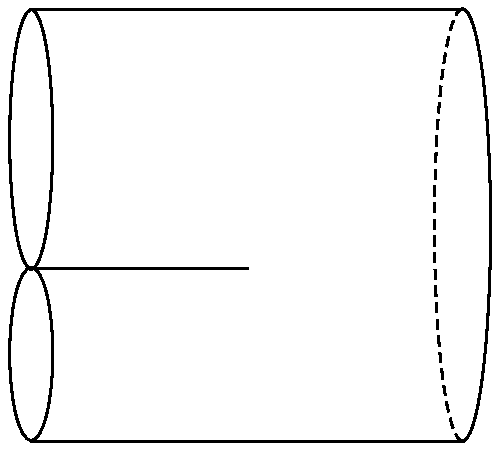
\includegraphics[width=.2\textwidth]{figures/LCcubic.pdf}}
\caption{The lightcone gauge worldsheet diagram representing the tree-level $2\to 1$ amplitude.}\label{LCcubic}
\end{figure}

We can also derive the lightcone prescription for the $2\to 1$ amplitude from the covariant formulation of the string amplitude. As in section \ref{superstringtree}, the asymptotic string states are represented by the $(-1,-1)$ picture vertex operators of the form
\ie
{\cal V}(k,\zeta,\wt\zeta) = c\widetilde c e^{-\phi-\widetilde\phi} V^{\rm m}(k,\zeta,\wt\zeta),~~~~  V^{\rm m}(k,\zeta,\wt\zeta) \equiv g_s  (\zeta\cdot \psi) (\wt\zeta\cdot\widetilde\psi) e^{ik\cdot X},
\fe
with the BRST-closure condition 
\ie
k^2 \equiv -2k^+ k^- + (k^\perp)^2=0,~~~~ k\cdot \zeta = k\cdot \wt\zeta=0.
\fe
The covariant tree-level $2\to 1$ massless (NS,NS) string amplitude can be expressed as
\ie\label{covathrpt}
{\cal A}_{\rm cov} = \left\langle c\widetilde c e^{-\phi-\widetilde\phi} V^{\rm m}(k_3,\zeta_3,\wt\zeta_3)(\infty) {\cal X}\wt{\cal X}(t_1)  c\widetilde c e^{-\phi-\widetilde\phi} V^{\rm m}(k_1,\zeta_1,\wt\zeta_1)(0) c\widetilde c e^{-\phi-\widetilde\phi} V^{\rm m}(k_2,\zeta_2,\wt\zeta_2)(1)\right\rangle,
\fe
where we have chosen to insert the vertex operators at $t = 0,1,\infty$ on the Riemann sphere, and the picture changing operators ${\cal X}$, $\wt{\cal X}$ at $t=t_1$. Of course, the BRST invariance ensures that the resulting amplitude is independent of these choices. 

For comparison with (\ref{liftcorrthr}), we will specialize to polarization vectors
$\zeta_i = (\zeta_i^+, \zeta_i^-, \zeta_i^\perp)$ of the form
\ie\label{zetalighcones}
\zeta_i^+ = 0, ~~~ \zeta_i^- = {k_i^\perp\cdot \zeta_i^\perp\over k_i^+},
\fe
and so
\ie\label{vrmakka}
V^{\rm m}(k_i, \zeta_i, \wt \zeta_i) = g_s\,  \zeta_i^\perp\cdot \Big(\psi^\perp - {k_i^\perp\over k_i^+} \psi^+\Big) \, \wt\zeta_i^\perp\cdot \Big(\wt\psi^\perp - {k_i^\perp\over k_i^+} \wt\psi^+\Big)\, e^{ik_i^\perp\cdot X^\perp - ik_i^- X^+ - ik_i^+ X^-}.
\fe
The holomorphic PCO can be expressed as (adopting $\A'=1$ convention)
\ie\label{pcolcgas}
{\cal X} = -{1\over 2} e^\phi \left( G^\perp - i \sqrt{2} \psi^- \partial X^+ - i \sqrt{2} \psi^+ \partial X^- \right) + c \partial \xi - {1\over 4} e^{2\phi} \partial \eta b - {1\over 4} \partial (e^{2\phi} \eta b ),
\fe
where $G^\perp = i \sqrt{2} \psi^i \partial X^i$ is the same as the $G$ appearing in (\ref{liftcorrthr}). The pure ghost terms as well as the term involving $\psi^+$ in (\ref{pcolcgas}) do not contribute to (\ref{liftcorrthr}). The term involving $\psi^-\partial X^+$ in (\ref{pcolcgas}) can only contribute through the contraction of $\partial X^+$ with an $X^-$ from one of the three massless (NS,NS) vertex operators, which is proportional to 
\ie\label{ktkta}
{k_1^+\over t_1} + {k_2^+\over t_1 - 1}.
\fe
On the other hand, according to (\ref{knrelas}) and (\ref{thrptcovmap}), $t_1 = {k_1^+\over k_1^+ + k_2^+}$, and so (\ref{ktkta}) in fact vanishes. Therefore only the term involving $G^\perp$ in the PCO (\ref{pcolcgas}) contributes to (\ref{liftcorrthr}), and consequently the terms involving $\psi^+, \wt\psi^+$ in (\ref{vrmakka}) also drop out. The relevant $\B\C$ system correlator evaluates to
\ie\label{bcmstcorr}
\left\langle e^{-\phi-\widetilde\phi}(\infty) e^{\phi+\wt\phi}(t_1)  e^{-\phi-\widetilde\phi}(0) e^{-\phi-\widetilde\phi} (1) \right\rangle_{\B\C} = |t_1(t_1-1)|^2 = {(k_1^+)^2 (k_2^+)^2\over (k_3^+)^4} .
\fe 
The amplitude (\ref{covathrpt}) thus reduces to
\ie\label{covathrptsimp}
{\cal A}_{\rm cov} &= - i (2\pi)^2 \delta(k^+ - k_1^+ - k_2^+) \delta(k^- - k_1^- - k_2^-) \, 2\pi g_s {(k_1^+)^2 (k_2^+)^2\over (k_3^+)^4}
\\
&~~~ \times \bigg\langle \zeta_3^\perp\cdot \psi^\perp \wt\zeta_3^\perp\cdot \wt\psi^\perp e^{ik_3^\perp\cdot X^\perp }(\infty) \, G^\perp\wt G^\perp(t_1) 
\\
&~~~~~~~~~~  \zeta_1^\perp\cdot \psi^\perp \wt\zeta_1^\perp\cdot \wt\psi^\perp e^{ik_1^\perp\cdot X^\perp }(0) \,\zeta_2^\perp\cdot \psi^\perp \wt\zeta_2^\perp\cdot \wt\psi^\perp e^{ik_2^\perp\cdot X^\perp }(1) \bigg\rangle_{X^\perp,\psi^\perp} .
\fe
Recall that $g_s$ is related to $g_A$ by (\ref{giiadef}). The correlator of the transverse fields $X^\perp,\psi^\perp$ in (\ref{covathrptsimp}), which contains the entire polarization and transverse momentum dependence, agrees with that of (\ref{liftcorrthr}). Furthermore, the additional factors involving $k_i^+$ coming from the $\B\C$ system correlator (\ref{bcmstcorr}) agrees with the $N_1, N_2$ dependence of ${\cal A}_{\rm MST}$ (\ref{amstfirthr}) including that of the conformal anomaly factor (\ref{cnnresann}). This suggests that ${\cal A}_{\rm MST}$ can be identified with ${\cal A}_{\rm cov}$ for the lightcone momentum assignment (\ref{knrelas}), with $X^-$ compactified on a circle of unit radius, namely
\ie\label{mstcovaa}
{\cal A}_{\rm MST} = {{\cal A}_{\rm cov} \over \delta(k_3^+ - k_1^+ - k_2^+)}\bigg|_{k_1^+=N_1, k_2^+=N_2, k_3^+=N}.
\fe
This identification then fixes the coefficient $a_0$ of the DVV twist field in (\ref{dvvdefma}) to be
\ie\label{azerodof}
a_0 = %- 2^{11\over 2} \pi^3 .
-2^{5\over 2} \pi^{3\over 2}.
\fe

%The polarization and transverse momentum dependence of ${\cal A}_{\rm cov}$, which comes entirely from the last factor of (\ref{covathrptsimp}), is in precise agreement with that of ${\cal A}_{\rm MST}$ (\ref{amstfirthr}), (\ref{liftcorrthr}).


 







\subsubsection{The matrix string theory conjecture}


Analogously to the BFSS conjecture (\ref{bfssconjforms}), a natural proposal is that the correspondence between the leading order matrix string theory amplitude and the type IIA string amplitude (\ref{mstcovaa}) should hold in the $N\to \infty$ limit for any $n$-point scattering amplitude, to all orders in perturbation theory with respect to the string coupling $g_A$ (\ref{gagymcorr}) (related to conformal perturbation theory coupling via (\ref{dvvdefma}), (\ref{azerodof})), and conceivably at the non-perturbative level as well.

At least in the perturbation theory, one expects a basis of asymptotic in- or out-states of matrix string theory to be labeled by those of the ${\rm Sym}^N(\mathbb{R}^8)$ SCFT, generalizing (\ref{nksinglstr}), (\ref{nksinglstrtwo}), in correspondence with free type IIA string states. For instance, an asymptotic state of $n$ gravitons $|N_1, k_1^\perp, e_1;\cdots; N_n, k_n^\perp, e_n \rangle^{in/out}$ is labeled by the lightcone momenta $k_i^+ = N_i$, $k_i^- = {(k_i^\perp)^2\over 2N_i}$, transverse momenta $k_i^\perp$, and polarization tensor $e_{i\mu\nu} = \zeta_{i\mu} \wt\zeta_{i\nu}$ where $\zeta_i$ is of the form (\ref{zetalighcones}), $i=1,\cdots, n$, with $\sum_{i=1}^n N_i = N$. The matrix string amplitude ${\cal A}_{\rm MST}$ is defined as the overlap between in and out basis states,
\ie
{\cal A}_{\rm MST}(\{N_i, k_i^\perp, e_i\}; \{N_j', k_j'^\perp, e_j'\}) = {}^{out}\left\langle \{N_i, k_i^\perp, e_i\} | \{ N_j', k_j'^\perp, e_j'\} \right\rangle^{in},
\fe
and can be decomposed in terms of the connected amplitudes ${\cal A}_{\rm MST}^{\rm conn}$ via (\ref{conncluster}). We will write ${\cal A}_{\rm cov}^{\rm conn}$ for the connected amplitude of the corresponding asymptotic states in the type IIA string theory. The matrix string theory conjecture can be formulated as the relation
\ie\label{mstcovafull}
\lim_{N\to \infty}{1\over \C N} {\cal A}_{\rm MST}^{\rm conn}(\{N_i = \C N k_i^+, k_i^\perp, e_i\}; \{N_j' = \C N k_j'^+, k_j'^\perp, e_j'\}) = {{\cal A}_{\rm cov}^{\rm conn}(\{ k_i, e_i\}; \{ k_j', e_j'\}) \over \delta(\sum_i k_i^+ - \sum_j k_j'^+ )},
\fe
where $\C$ is an arbitrary positive constant (boost factor). A nontrivial check of this proposal in the case of the tree-level 4-graviton amplitude has been performed in Arutyunov and Frolov, Nucl. Phys. B \textbf{524} (1998), 159 \cite{Arutyunov:1997gi}.










\appendix 



\newpage

\section{Frequently used formulae and conventions}

\noindent $\bullet$ 2D CFT

%- $TT$ OPE (\ref{ttopes}) and Virasoro algebra (\ref{viralgresa})

%- Weyl anomaly (\ref{trwelan})

- free boson convention (\ref{xxactfbs}), (\ref{xxop}), (\ref{xoope}), (\ref{clstr})

- free fermion convention (\ref{psipmconvac}), (\ref{psicylex}), (\ref{frepsiact}), (\ref{psiopenc}), (\ref{tpsica})


- $\B\C$  re-bosonization dictionary (\ref{bcdict}), (\ref{thetabetadic})



- 2D ${\cal N}=1$ superconformal algebra (\ref{ggope})

- 2D ${\cal N}=2$ superconformal algebra (\ref{ntwoscarel})

\noindent $\bullet$ BRST 

- $j_B$ and $Q_B$ in bosonic string theory (\ref{jbexpex}), (\ref{qosc})

- $j_B$ and $Q_B$ in superstring theory (\ref{jbrstbetgams}), (\ref{jbrstetaxis}), (\ref{qblsuper})




\noindent $\bullet$ Picture changing operator

- PCO in $\B\C$ representation (\ref{pcoregdef})

- PCO in $(\phi,\eta,\xi)$ representation (\ref{pcophixieta})

\noindent $\bullet$ String amplitudes

- general bosonic amplitude (\ref{omegaone}), (\ref{normconsts})

- normalization of bosonic worldsheet correlator (\ref{eikxcorrconv}), (\ref{ccoresign})

- general type II string amplitude (\ref{superamp}), (\ref{omegasupercorr}), (\ref{nhmsuperss}), (\ref{superamppco}), (\ref{supintegrand})

- normalization of type II worldsheet correlator (\ref{nomconvtyii})

- general open bosonic amplitude (\ref{openampbos}), (\ref{nhbnmbos})

- normalization of open bosonic worldsheet correlator (\ref{discnorm}), (\ref{ndtwon}), (\ref{gsgorel})

- open type II string amplitude (\ref{openclosedsupamp}), (\ref{normopensup})

- normalization of open type II worldsheet correlator (\ref{discnormsup}), (\ref{ndtwosup}), (\ref{gsgosup})


\noindent $\bullet$ Gravitational and gauge coupling constants

- $\kappa$ in bosonic string theory (\ref{kapgsbos})

- $\kappa$ in type II string theory (\ref{typeiigskap})

- $\kappa$ and $g_{\rm YM}$ in heterotic string theory (\ref{kappahetconvs}), (\ref{hetcouprel})

- $\kappa$ and $g_{\rm YM}$ in type I string theory (\ref{kappagymtypei})

\noindent $\bullet$ Open and closed string couplings

- $g_o$ vs $g_s$ in bosonic string theory (\ref{gsgorel})

- $g_o$ vs $g_s$ in type II string theory (\ref{gsgosup})

- dimensionless type II string coupling (\ref{giibdef}), (\ref{giiadef})

- dimensionless heterotic and type I string coupling (\ref{dimlesseoi})

\noindent $\bullet$ D-brane tension

- $T_p$ in bosonic string theory (\ref{gotprels}), (\ref{tpkapbos})

- $T_p$ in type II theory (\ref{tpkapsup})


\noindent $\bullet$ Supergravity

- spin connection (\ref{spinconndef}), (\ref{spinconndefom})

- 11D supersymmetry variation (\ref{epsitr})

- IIA supersymmetry variation (\ref{iiasugravar})

- IIB supersymmetry variation in string frame (\ref{iibsusyvar}), Einstein frame (\ref{susyeincomp})

- type I supersymmetry variation (\ref{susyvartypei})

\noindent $\bullet$ Gravitational solutions

- black $p$-branes (\ref{blackpbranemetric}), (\ref{blackpbranephif}), (\ref{fprsol})

- NS5-brane in type II string theory (\ref{nsfivesol}), (\ref{nsfivesol})

- NS5-brane in heterotic string theory (\ref{strnsfivehet}), (\ref{hphisol}), (\ref{aixynmhetnsf}), (\ref{ephisol})

- M-branes (\ref{balcmtws}), (\ref{mfivesolsug})

- D1-D5 system (\ref{oneficbranebl})

- conifold (\ref{conifoldmetric}), deformed (\ref{dsactdefo}), resolved (\ref{resconmet})

\noindent $\bullet$ String field theory

- closed bosonic SFT classical action (\ref{classicalsftact}), EOM (\ref{clsfteom}), quantum BV action (\ref{bvsftfnl})

- closed superstring field theory action (\ref{bvsftfnlsuper})

- classical open bosonic SFT action in cubic form (\ref{cubicbv}), tachyon vacuum solution (\ref{tvkbc})

- open+closed SFT action bosonic (\ref{oncact}), type II (\ref{bvsftfnlsuperoc})

\noindent $\bullet$ M-theory

- 11D gravitational coupling and Planck mass (\ref{kappamelev})

- M2 and M5-brane tensions (\ref{tmtwo}), (\ref{tmfifoa})

\noindent $\bullet$ AdS/CFT

- AdS$_5\times S^5$ coupling and radius (\ref{paradiction})

- boundary to bulk propagator for scalar (\ref{scalsole}), gauge field (\ref{amusols}), graviton (\ref{gravsols})

- ${\cal N}=4$ SYM action (\ref{nfouract})

- AdS$_4\times \mathbb{CP}^3$ solution (\ref{adscpthsols}), coupling and radius (\ref{adscpthcourad})

- ABJM action (\ref{abjmaction})

- AdS$_3\times S^3\times M_4$ solution pure RR case (\ref{datadsthrmff}), (\ref{attrhorvol}), pure NSNS case (\ref{parapurensns})

\noindent $\bullet$ Integrability

- magnon dispersion relation and spectral parameters (\ref{hmagdisp}), (\ref{xpmdefeqn}), (\ref{uvardef})

- $su(2|2)$ magnon S-matrix (\ref{tbodyssmat}), (\ref{abcdkl})

- the dressing factor (\ref{crossansaz}), (\ref{chixy}), DHM representation (\ref{dhmint})

- mirror TBA (\ref{mirtbagennu})

- $Y$-functions (\ref{zetaysysdef}), (\ref{yfuncredef}), analyticity property (\ref{analstrip}), (\ref{ywwtinvert})

- quantum spectral curve (${\bf P}\mu$-system) (\ref{pmuone}), (\ref{pmutwo}), asymptotic condition (\ref{pmuasymps})

%\noindent $\bullet$ spinor conventions


%\noindent $\bullet$ ${\cal N}=4$ SYM



%- superconformal algebra



\newpage

\section{The path integral}

\subsection{Path integral formulation of quantum mechanics}

Consider a quantum mechanical system of $D$ degrees of freedom, with canonical coordinates $\hat q^a$ and momenta $\hat p_a$ that obey the canonical commutation relations $[\hat q^a ,\hat p_b] = i \delta^a_b$. The position eigenbasis $|q\rangle$ and the momentum eigenbasis $|p\rangle$ are related by $\langle q|p\rangle = e^{ip\cdot q}$, with $\int d^Dq |q\rangle\langle q| = \int {d^Dp\over (2\pi)^D}|p\rangle\langle p|=1$. The matrix elements of the time-evolution operator $U(T) = \exp(-i \hat H T)$ in the position eigenbasis can be expressed as
\ie\label{pathinta}
\langle q_f| U(T) |q_i\rangle = \int \prod_{n=1}^{N-1} {d^D q_n} \prod_{n=0}^{N-1} { d^D p_n\over (2\pi)^D} \langle q_{n+1}|p_n\rangle \langle p_n | U(\tfrac{T}{N}) |q_n\rangle,
\fe
where we have set $q_N\equiv q_f$, $q_0\equiv q_i$. For large $N$, one may write
\ie
\langle p_n | U(\tfrac{T}{N}) |q_n\rangle = \exp\left(-i H(q_n,p_n) \tfrac{T}{N}\right) \langle p_n|q_n\rangle,
\fe
where $H(q,p)$ is an ordinary function of $q, p$ that may be viewed as a classical Hamiltonian, and re-express (\ref{pathinta}) as
\ie\label{dischampath}
\langle q_f| U(T) |q_i\rangle = \int \prod_{n=1}^{N-1} {d^D q_n} \prod_{n=0}^{N-1} { d^D p_n\over (2\pi)^D} \exp\left\{ i \sum_{n=0}^{N-1} \Big[ p_n\cdot (q_{n+1} - q_n) - H(q_n,p_n) \tfrac{T}{N} \Big] \right\}.
\fe 
Formally taking the $N\to \infty$ ``limit'' yields the functional integral
\ie\label{pathinteqm}
\int Dq Dp\, \exp\left[ i \int_0^T dt \left(p\cdot \dot q - H(q,p) \right) \right].
\fe
Generally, the functional integral integration measure $Dq Dp$ should be viewed as defined by a regularization, such as discretization of time as in the above derivation, or a cutoff in frequency space which is often more convenient for computations. The different regularization schemes lead to expressions for $H(q,p)$ that differ by the so-called counter terms.

When $H(q,p)$ is quadratic in $p$, e.g.
\ie\label{hpqsigma}
H(q,p) = {1\over 2} G^{ab}(q) p_a p_b + V(q),
\fe
one can perform the Gaussian integration with respect to $p(t)$ in (\ref{pathinteqm}), yielding the Lagrangian form of the path integral
\ie\label{pathintlag}
\int [Dq] \exp\left[ i\int_0^T dt L(q,\dot q) \right],
\fe
where $L$ is related to $H$ by the Legendre transform
\ie
L(q,\dot q) = \left(p\cdot \dot q - H(p,q) \right)\Big|_{\dot q = {\partial H\over \partial p}} = {1\over 2} G_{ab}(q) \dot q^a \dot q^b - V(q),
\fe
where $G_{ab}$ is the inverse matrix of $G^{ab}$ appearing in (\ref{hpqsigma}). The measure $[Dq]$ appearing in (\ref{pathintlag}), in the time-discretization scheme of (\ref{dischampath}), is
\ie
[Dq] = \left(2\pi i \tfrac{T}{N}\right)^{-{N\over 2}} \prod_{n=0}^{N-1} {d^D q_n} \sqrt{\det (G_{ab}(q_n))}.
\fe

\subsection{Path integral with Grassmann-odd field variables}
\label{sec:grassmannpathint}

Now consider Grassmann-odd canonical coordinates $\eta_\A$, $\A=1,\cdots, D$, that obey $\eta_\A\eta_\B=-\eta_\B\eta_\A$ and $\eta_\A^2=0$. As the odd variables cannot be assigned values, the configuration space must be viewed as an abstract ringed space that is characterized through the ring of functions $f(\eta_\A)$. Consider the Lagrangian
\ie
L = \sum_{\A,\B=1}^D M_{\A\B} \eta_\A \dot\eta_\B,
\fe
where $M_{\A\B}$ is a symmetric matrix. The canonical momentum conjugate to $\eta_\A$ is
\ie
\pi_\A = L {\overleftarrow\partial\over \partial \dot\eta_\A} = M_{\A\B} \eta_\B.
\fe
The algebraic relation between $\pi_\A$ and $\eta_\B$,
\ie\label{chiacons}
\chi_\A(\eta, \pi) \equiv \pi_\A - M_{\A\B} \eta_\B = 0,
\fe
is a {\it second-class primary constraint} in the terminology of Dirac.\footnote{Dirac, {\it Lectures on Quantum Mechanics}, 1964. The term ``second-class'' refers to the property that $\chi_\A$ have non-degenerate Poisson brackets among themselves, which is in contrast to the ``first-class'' constraints that have to do with gauge redundancy. The term ``primary'' is in contrast to ``secondary'' constraints which are the constraints that follow from the equation of motion.} Rather than working with the Poisson bracket defined by
\ie
\{\eta_\A, \eta_\B\}_{\rm P} = 0 = \{\pi_\A, \pi_\B\}_{\rm P},~~~~ \{\eta_\A, \pi_\B\}_{\rm P} = \delta_{\A\B} = \{\pi_\A, \eta_\B\}_{\rm P},
\fe
which is incompatible with the constraints (\ref{chiacons}), one considers the (classical) Dirac bracket defined by
\ie
\{ f, g \}_{\rm D} := \{ f, g \}_{\rm P} - \{ f, \chi_\A \}_{\rm P} (K^{-1})^{\A\B} \{\chi_\B, g\}_{\rm P},
\fe
where $K^{-1}$ is the inverse matrix of 
\ie
K_{\A\B} \equiv \{\chi_\A, \chi_\B\}_{\rm P} = - 2 M_{\A\B}.
\fe
The Dirac bracket is compatible with the constraints as $\{f, \chi_\A\}_{\rm D}=0$ for any $f$. Note that we have in particular
\ie
\{\eta_\A, \eta_\B\}_{\rm D} = {1\over 2} (M^{-1})_{\A\B}, ~~~~ \{\eta_\A, \pi_\B\}_{\rm D} = {1\over 2} \delta_{\A\B}.
\fe

The quantization of the Grassmann-odd mechanical system is defined by promoting $\eta_\A$ to an (ordinary) linear operator $\hat\eta_\A$ that acts on a Hilbert space ${\cal H}$, such that
\ie
\{ \hat\eta_\A, \hat\eta_\B\} = i {1\over 2} M_{\A\B}.
\fe
As an example, consider the $D=2$ system with the Lagrangian
\ie
L = i \sum_{\A=1}^2 \eta_\A \dot \eta_\A - i \omega \eta_1 \eta_2,
\fe
whose corresponding Hamiltonian is
\ie
H = \sum_{\A=1}^2 \pi_\A \dot \eta_\A - L = i \omega \eta_1 \eta_2.
\fe
Upon quantization, we have the operators $\hat\eta_1, \hat\eta_2$ that obey
\ie
\hat\eta_1^2 = \hat \eta_2^2 = {1\over 4}, ~~~~ \{\hat\eta_1, \hat\eta_2\}=0.
\fe
A minimal choice is ${\cal H}\simeq \mathbb{C}^2$, with 
\ie
\hat\eta_1 = {1\over 2} \sigma_1,~~~~ \hat\eta_2 = {1\over 2} \sigma_2,~~~~\hat H = i\omega \hat\eta_1 \hat\eta_2 = -{\omega\over 4} \sigma_3,
\fe
where $\sigma_i$ are Pauli matrices. 

For a two-state quantum system with basis $|0\rangle, |1\rangle$, consider the pair of operators $\hat\eta, \hat\chi$ defined by
\ie
\hat\eta|0\rangle = \hat\chi|1\rangle =0,~~~~ \hat\eta|1\rangle = |0\rangle,~~~~ \hat\chi|0\rangle = |1\rangle.
\fe
The ``position eigenstate'' 
\ie
|\eta\rangle \equiv |1\rangle \eta + |0\rangle,
\fe
where $\eta$ is a formal Grassmann-odd {\it coordinate}, obeys
\ie
\hat\eta|\eta\rangle = |0\rangle \eta = |\eta\rangle \eta.
\fe
We will also define the bra-state
\ie
\langle \langle \chi| \equiv -\langle 1| + \chi \langle 0|, 
\fe
for a formal Grassmann-odd coordinate $\chi$, with the property
\ie
\langle\langle \chi | \eta\rangle = \chi - \eta, ~~~~ \langle\langle \chi|\hat\eta = \chi \langle 1| = -\chi \langle\langle \chi|.
\fe
The Grassmann/Berezin integral $\int d\eta$ is defined by
\ie
\int d\eta \, \eta = 1,~~~~\int d\eta \,1 = 0.
\fe
By convention we will write $\eta\, d\eta = -d\eta\, \eta$. It follows that we have the completeness relation
\ie\label{complegras}
\int |\eta\rangle d\eta \langle\langle \eta| &= \int d\eta |-\eta\rangle \langle\langle \eta|
\\
&= \int d\eta (-|1\rangle \eta + |0\rangle) (-\langle 1| + \eta\langle 0|)
\\
& = |1\rangle\langle 1| + |0\rangle\langle 0| = 1.
\fe
The matrix element of the time evolution operator $U(T) = \exp(-i \hat H T)$ between a pair of bra and ket position eigenstates can now be expressed as
\ie\label{graspatha}
\langle\langle \eta_f | U(T) |\eta_i\rangle = \int \langle\langle \eta_f | U(\tfrac{T}{N}) | \eta_{N-1} \rangle d\eta_{N-1}\langle\langle \eta_{N-1}| \cdots \cdots |\eta_1\rangle d\eta_1 \langle\langle \eta_1 | U(\tfrac{T}{N}) |\eta_i\rangle.
\fe
For large $N$, we may write
\ie
\langle\langle \eta_{n+1} | U(\tfrac{T}{N}) |\eta_n\rangle = - \int d\chi_n \exp\left[ - i H (\chi_n, \eta_n) \tfrac{T}{N} - \chi_n (\eta_{n+1} - \eta_n) \right],
\fe
where $H(\chi, \eta)$ is an analytic function of $\chi, \eta$ defined by its Taylor series, and re-express (\ref{graspatha}) as
\ie
\langle\langle \eta_f | U(T) |\eta_i\rangle = - \int d\chi_0 \prod_{n=1}^{N-1} d\eta_n d\chi_n \,\exp\left\{ \sum_{n=0}^{N-1} \Big[ -i H(\chi_n, \eta_n) \tfrac{T}{N} - \chi_n (\eta_{n+1} - \eta_n) \Big] \right\},
\fe
where we have set $\eta_N\equiv \eta_f$, $\eta_0 \equiv \eta_i$.
Formally taking the $N\to \infty$ limit then yields the Grassmann path integral
\ie\label{grasspathint}
\int D\eta D\chi\, \exp\left\{ \int_0^T dt \left[ - \chi \dot\eta - i H (\chi, \eta) \right] \right\}.
\fe
Note that there is no distinction between the Hamiltonian and Lagrangian form of the Grassmann path integral:
the exponent appearing in (\ref{grasspathint}) can be written as $i S$, where $S$ is the action
\ie
S = \int dt \, L,~~~~ L = i \chi \dot\eta - H(\chi, \eta).
\fe

The thermal partition function at inverse temperature $\B$ can be written as
\ie\label{themfermpa}
Z(\B) &= {\rm Tr}_{\cal H} e^{-\B \hat H} = \int {\rm Tr}_{\cal H} |\eta\rangle d\eta \langle\langle \eta | e^{-\B\hat H}
\\
&= \int  d\eta \langle\langle \eta | e^{-\B\hat H}  |-\eta\rangle.
\fe
The flip of sign on $\eta$ is due to moving $|\eta\rangle$ to the right of $d\eta$, as seen in (\ref{complegras}). As a consequence, the thermal partition function is computed by the functional integral over $\eta(\tau)$, where $\tau$ is the Euclidean time related to real time $t$ by $t=-i\tau$, that obeys the anti-periodic boundary condition $\eta(\tau+\B) = -\eta(\tau)$.



\subsection{Tunneling and instantons}
\label{sec:bounce}

Consider the quantum mechanical model (\ref{hpqsigma}), where the potential $V(q)$ is taken to be of the form
\ie\label{vqhpot}
V(q) = {1\over 2} G^{ab}(q) {\partial h(q)\over \partial q^a} {\partial h(q)\over \partial q^b} ,
\fe
for a function $h(q)$ which we will refer to as the Morse function. $V(q)$ acquires minimal value 0 at a critical point of $h(q)$, i.e. where $\partial_a h(q) = 0$. Suppose that there are several critical points $q_\A$, $\A=1,2,\cdots$. In the classical limit, the lowest energy states $|\A\rangle$ are characterized by wave functions localized at $q\approx q_\A$. The quantum tunneling leads to nonzero matrix elements of the propagator between these states,
\ie\label{albrmatel}
\langle \B| e^{- H T} |\A\rangle = \sum_n e^{-E_n T} \langle \B|n\rangle \langle n|\A\rangle,
\fe
where $\{|n\rangle\}$ is an orthonormal basis of energy eigenstates with energy $E_n$.
In the case of one degree of freedom, this can be analyzed using the WKB approximation. More generally, the matrix element (\ref{albrmatel}) can be formulated as the Euclidean path integral
\ie\label{albepath}
\langle \B| e^{- H T} |\A\rangle = \int [Dq]\Big|_{q(-{T\over 2})=q_\A}^{q({T\over 2})= q_\B} e^{- S^{\rm E}[q]},
\fe
where the Euclidean action $S^{\rm E}[q]$ is related to $L(q,\dot q)$ of (\ref{pathintlag}) by
\ie
S^{\rm E}[q]\equiv \int_{-{T\over 2}}^{T\over 2} d\tau L^{\rm E}(q, \partial_\tau q),~~~~
L^{\rm E}(q, \partial_\tau q) = -L(q, i\partial_\tau q).
\fe
In the model (\ref{hpqsigma}) with (\ref{vqhpot}), $S^{\rm E}[q]$ subject to the boundary condition $q(-{T\over 2}) = q_\A$, $q({T\over 2}) = q_\B$ can be written as
\ie
S^{\rm E} &= \int_{-{T\over 2}}^{T\over 2} d\tau \left[ {1\over 2} G_{ab}(q) \partial_\tau q^a \partial_\tau q^b +  {1\over 2} G^{ab}(q) {\partial h(q)\over \partial q^a} {\partial h(q)\over \partial q^b} \right]
\\
&= \int_{-{T\over 2}}^{T\over 2} d\tau  {1\over 2} G_{ab}(q) \left( \partial_\tau q^a \pm G^{ac}(q)\partial_{q^c} h(q) \right)  \left( \partial_\tau q^b \pm G^{bd}(q)\partial_{q^d} h(q) \right)  
\\
&~~~~ \mp \left[ h(q_\B) - h(q_\A) \right] .
\fe
In particular, in the $T\to \infty$ limit, the action is minimized by the solutions to the first order differential equation
\ie\label{qsteascn}
\partial_\tau q^a \pm G^{ac}(q)\partial_{q^c} h(q) = 0, 
\fe
where the sign is $+$ (or $-$) for $h(q_\B)<h(q_\A)$ (or $h(q_\B)>h(q_\A)$), with $q(-\infty) = q_\A$, $q(+\infty) = q_\B$. Note that (\ref{qsteascn}) represents the steepest descent (ascent) path from $q_\A$ to $q_\B$ with respect to the Morse function $h(q)$. These solutions will be referred to as ``instantons'' or ``bounces''.

For large but finite $T$, the above instanton solution does not quite satisfy the boundary condition, but nonetheless approximates a saddle point of the path integral, on which the Euclidean action evaluates to
\ie
S^{\rm E} \approx S_{\B\A} \equiv |h(q_\B) - h(q_\A)|.
\fe
In the semi-classical approximation, it will also be necessary to calculate the Gaussian (i.e. 1-loop) functional determinant of fluctuations around the instanton, which is further complicated by the presence of a zero mode that corresponds to the time translation of the instanton. We will defer a more careful analysis to the next section in the context of a supersymmetric model, and for now simply assume that the Gaussian functional determinant of the nonzero modes gives rise to a factor $K_{\B\A}$, whereas the integration over the zero mode associated with time translation gives a factor $T$. The instanton contribution to (\ref{albepath}) is then $e^{-S_{\B\A}} K_{\B\A} T$, from which we conclude
\ie\label{betalpsplit}
\langle \B| H |\A\rangle \approx e^{-S_{\B\A}} K_{\B\A} .
\fe
To recover the spectral decomposition (\ref{albrmatel}), it will be necessary to sum up the contributions from the approximate saddle points that correspond to a sequence of alternating instanton and anti-instantons at large separation in Euclidean time (this is often referred to as the ``instanton gas'').


%\ie
%\langle \B| e^{- H T} |\A\rangle &\approx \sum_{n=0}^\infty \int_{-{T\over 2}<\tau_1<\cdots < \tau_n < {T\over 2}} d\tau_1\cdots d\tau_n \left(e^{-S_{\B\A}} K_{\B\A} \right)^{2n+1}
%\\
%& = {1\over 2} \exp\left(e^{-S_{\B\A}} K_{\B \A} T \right) - {1\over 2} \exp\left( - e^{-S_{\B\A}} K_{\B \A} T \right) .
%\fe



\subsection{A supersymmetric model}

Let $M$ be an $N$-dimensional Riemannian manifold parameterized by the coordinates $x^i$, whose metric is written as
$ds^2 = g_{ij}(x) dx^i dx^j$. We can express $g_{ij}(x) = \sum_{a=1}^N e^a{}_i(x) e^a{}_j(x)$, where
the matrix $e^a{}_i$ defines a local frame. The inverse matrix of $e^a{}_i$ will be denoted $e_a{}^i$, i.e. $e_a{}^i e^b{}_i = \delta_a^b$, $e_a{}^i e^a{}_j = \delta^i_j$. Let $\eta^a$ and $\overline\eta{}^a$, $a=1, \cdots, N$, be a set of Grassmann-odd variables, and define
\ie
\psi^i \equiv e_a{}^i(x) \eta^a,~~~~ \overline\psi{}^i \equiv e_a{}^i(x) \overline\eta^a,
\fe
which are invariant under the $O(N)$ rotations simultaneously of the frame and of $\eta^a, \overline\eta{}^a$. A classical mechanical system is defined by viewing the coordinates $x^i$, their conjugate momenta $p_i$, and $\eta^a, \overline\eta{}^a$ as phase space variables. The Poisson bracket between the Grassmann-odd variables is defined as $\{ \eta^a, \eta^b \}_{\rm P} = \{ \overline\eta{}^a, \overline\eta{}^b \}_{\rm P} = 0$, $\{ \eta^a, \overline\eta{}^b \}_{\rm P} = -i \delta^{ab}$,
and the Poisson brackets between $(\eta^a, \overline\eta{}^a)$ and $(x^i, p_i)$ vanish.

Via canonical quantization, a quantum system is defined by promoting $x^i, p_i, \eta^a, \overline\eta^a$ to operators, among which the non-vanishing (anti-)commutators are
\ie
[x^i, p_j] = i \delta^i{}_j, ~~~~ \{\eta^a, \overline\eta{}^b\} = \delta^{ab}.
\fe
A quantum state can be characterized by its wave function of the form
\ie\label{phixetawnv}
\Phi(x, \eta) \equiv \sum_{p=0}^N {1\over p!} \hat\Phi_{a_1\cdots a_p}(x) \eta^{a_1}\cdots \eta^{a_p}
= \sum_{p=0}^N {1\over p!} \Phi_{i_1\cdots i_p}(x) \psi^{i_1}\cdots \psi^{i_p},
\fe
where $\Phi_{i_1\cdots i_p} \equiv \hat\Phi_{a_1\cdots a_p} e^{a_1}{}_{i_1}\cdots e^{a_p}{}_{i_p}$ is anti-symmetric in its indices. A priori, (\ref{phixetawnv}) is well-defined at least when $\Phi_{i_1\cdots i_p}(x)$ is supported on the coordinate patch of $M$ where the coordinate system $x^i$ is non-degenerate. By linear superposition, it is straightforward to extend the notion of wave function to $\Phi_{i_1\cdots i_p}(x)dx^{i_1}\wedge \cdots \wedge dx^{i_p}$ a general differential $p$-form on $M$. The Hilbert space ${\cal H}$ is spanned by states defined through the differential $p$-forms on $M$, subject to the inner product
\ie\label{innersqmdef}
\langle \Phi_1 |\Phi_2\rangle &= \int d^N x \sqrt{\det g} \, \sum_{p=0}^N {1\over p!} \Phi_{1 a_1\cdots a_p}^*(x) \Phi_{2 a_1\cdots a_p}(x)
\\
&=  \int d^N x d^N \eta d^N \eta^* \sqrt{\det g} \, e^{\sum_{a=1}^N \eta^{a*} \eta^a} \sum_{p=0}^N {1\over p!} (\Phi_1(x,\eta))^\dagger \Phi_{2}(x,\eta).
\fe
In the second line, $\eta^{a*}$ are independent Grassmann-odd variables from $\eta^a$, the dagger is defined by complex conjugation combined with $(\eta^a \eta^b\cdots)^\dagger \equiv \cdots \eta^{b*} \eta^{a*}$, and the Berezin integration measure is normalized such that
\ie
\int d^N \eta d^N \eta^* \prod_{a=1}^N \eta^{a*} \eta^a = 1.
\fe
One can verify that with this definition of the inner product, the adjoint operator of $\eta^a$ is $\overline \eta{}^a = {\partial\over \partial \eta^a}$.

The operator $\widehat d$ is defined to act on the wave function as the exterior derivative on differential forms, namely
\ie
(\widehat d \Phi)(x,\eta) = \sum_{p=0}^N {1\over p!} \partial_j\Phi_{i_1\cdots i_p}(x) \psi^j \psi^{i_1}\cdots \psi^{i_p}.
\fe
It is not hard to verify that
\ie
\widehat d = \eta^a e_a{}^i ( \partial_i + \omega_{ib}{}^c \eta^b \overline\eta{}^c ),
\fe
where $\omega_{ib}{}^c = e_b{}^j (\partial_i e^c{}_{j} - \Gamma_{ij}^k e^c{}_{k})$ is the spin connection (see Appendix \ref{spinconn}). Next, we define the supercharge $Q\equiv - i \widehat d$. Explicitly, $Q$ and its adjoint $Q^\dagger$ can be expressed as
\ie\label{qqbarnlsm}
& Q = \eta^a e_a{}^i ( p_i - i \omega_{ibc} \eta^b \overline\eta{}^c ),
\\
& Q^\dagger = ( p_i^\dagger + i \omega_{ibc} \eta^c \overline \eta^b ) e_a{}^i \overline\eta^a
= \overline\eta{}^a e_a{}^i (p_i - i \omega_{ibc} \overline\eta^b \eta^c).
\fe
Note that the verification of the last equality requires some care, as $p_i =  - i \partial_i$ is not self-adjoint due to the measure factor in the definition of the inner product (\ref{innersqmdef}). We have $Q^2=(Q^\dagger)^2=0$, and will consider the Hamiltonian
\ie\label{hqqnlsm}
H = {1\over 2} \left\{ Q, Q^\dagger \right\}.
\fe
It is evident that the Hamiltonian acts on the wave function as ${1\over 2}$ times the Laplace-de Rham operator $\Delta = dd^\dagger + d^\dagger d$. In particular, $H$ is positive semi-definite, and its ground states correspond to harmonic forms on $M$.

One can verify through a bit of tedious calculation that the classical expression of the Hamiltonian is
\ie
H^{\rm cl} = {1\over 2} g^{ij} (p_i - i \omega_{iab} \eta^a \overline\eta{}^b) (p_j - i \omega_{jcd} \overline\eta{}^c \eta^d) - {1\over 2} R_{ijab} \overline\psi{}^a \psi^j \overline\eta{}^a \eta^b,
\fe
where $R_{ijab} \equiv R_{ijkl} e_a{}^k e_b{}^\ell = \partial_i \omega_{jab} - \partial_j \omega_{iab} + \omega_{iac} \omega_{jcb} - \omega_{jac} \omega_{icb}$. From this we can derive, via a Legendre transformation, the Lagrangian
\ie\label{lsqmclas}
L = {1\over 2} g_{ij}\dot x^i \dot x^j + {i\over 2} (\overline\eta{}^a\dot \eta^a + \eta^a \dot{\overline\eta}{}^a) + i \omega_{iab} \overline\eta{}^a \eta^b \dot x^i + {1\over 2} R_{abcd} \overline\eta{}^a \eta^b \overline\eta{}^c \eta^d.
\fe
The quantum system may be equivalently formulated through a path integral of the form
\ie
\int [Dx D\eta D\overline\eta] \exp\left({i\over \hbar} \int dt L\right),
\fe
where we have restored the $\hbar$ dependence. The Lagrangian appearing in the exponent may in principle differ from (\ref{lsqmclas}) by a counter term of order ${\cal O}(\hbar)$ that depends on the regularization scheme used to define the measure $[Dx D\eta D\overline\eta]$.

%It is useful to note that the path integral weight $\exp\left({i\over \hbar} \int dt L\right)$ is invariant under the scaling transformation
%\ie{}
%& \hbar \to \lambda \hbar,~~~ t\to \lambda t, ~~~ x^i \to x^i, ~~~\dot x^i \to \lambda^{-1} \dot x^i,~~~ \overline\eta{}^a \eta^b \to \lambda \overline\eta{}^a \eta^b,
%\\
%& g_{ij} \to \lambda^2 g_{ij},~~~ e^a{}_i \to \lambda e^a{}_i,~~~ \omega_{iab} \to \omega_{iab},~~~ R_{abcd} \to \lambda^{-2} R_{abcd}.
%\fe
%Provided that the regularization scheme is covariant with respect to reparameterization of $M$, any potential counter term must come with more time derivatives or additional powers of the curvature tensor.

The thermal partition function $Z(\beta) = {\rm Tr}_{\cal H} e^{-\B H}$, similarly to (\ref{themfermpa}), is calculated by the Euclidean path integral with anti-periodic boundary condition for the fermionic variables $\eta^a(\tau), \overline\eta^a(\tau)$ on the thermal circle. In the following we will consider the {\it Witten index}, defined as the partition function twisted by the fermion parity $(-)^F$, whose path integral representation involves periodic boundary condition for the fermionic variables, namely
\ie\label{wittnpathintt}
\wt Z(\B) &\equiv {\rm Tr}_{\cal H} (-)^F e^{-\B H} 
\\
&= \int [Dx D\eta D\overline\eta]\Big|_{\substack{\eta(\B) = \eta(0) \\ \overline\eta(\B) = \overline\eta(0)}} \exp\left(-{1\over \hbar} \int_0^\B d\tau L^{\rm E}\right),
\fe
where $L^{\rm E}$ is the Euclidean Lagrangian, defined as $-L$ with the Wick rotation $t\to -i\tau$.

Writing $Q_+\equiv {1\over \sqrt{2}}(Q+Q^\dagger)$ and so $H = Q_+^2$, with $\{(-)^F, Q_+\}=0$, we have
\ie\label{witindman}
{\partial\over \partial \B} \wt Z(\B) &= {\rm Tr}_{\cal H} \left[ (-)^F e^{-\B H} (-Q_+^2) \right]
\\
&=  {\rm Tr}_{\cal H} \left[ Q_+(-)^F e^{-\B H} (-Q_+) \right] ~~~~({\rm cyclicity~of~trace})
\\
&=  {\rm Tr}_{\cal H} \left[ (-)^F e^{-\B H} Q_+^2 \right] ~~~~({\rm using}~Q_+(-)^F=-(-)^F Q_+)
\fe
which must therefore vanish.\footnote{The application of cyclicity of trace in (\ref{witindman}) may fail when the energy spectrum is not gapped. As a toy example, take ${\cal H} = L^2(\mathbb{R})$, and consider ${\rm Tr} [p, f(x)] = - i \int dx \partial_x f(x) = -i (f(\infty) - f(-\infty))$ which can be nonzero. For a nontrivial example of the Witten index in a gapless system see Sethi and Stern, Commun. Math. Phys. \textbf{194}, 675 \cite{Sethi:1997pa}.} That is, $\wt Z(\B)$ is independent of $\B$, and only receives contribution from the supersymmetric ground states i.e. those annihilated by $Q_+$, namely
\ie
\wt Z(\B) = n_+ - n_-,
\fe
where $n_+$ and $n_-$ counts the number of ground states with $(-)^F = 1$ and $-1$ respectively.

By the following change of variable
\ie
\tau \equiv \B s, ~~~ \eta^a \equiv \B^{-{1\over 2}} \wt\eta^a,~~~ \overline\eta{}^a \equiv \B^{-{1\over 2}} \wt{\overline\eta}{}^a,
\fe
we can rewrite the functional integrand of (\ref{wittnpathintt}) as
\ie{}
& \exp\Bigg[ - {1\over \B\hbar} \int_0^1 \left( {1\over 2} g_{ij} \partial_s x^i \partial_s x^j + {1\over 2} \wt\eta^a \partial_s \wt\eta^a + {1\over 2}  \wt{\overline\eta}{}^a \partial_s \wt{\overline\eta}{}^a + \omega_{iab} \wt{\overline\eta}{}^a \wt\eta{}^b \partial_s x^i - {1\over 2} R_{abcd} \wt{\overline\eta}{}^a {\overline\eta}{}^b \wt{\overline\eta}{}^c {\overline\eta}{}^d \right) 
\\
& ~~~~~~~~ + {\cal O}(\B \hbar)~{\rm counter~terms}  \Bigg].
\fe
Here we have assumed that the functional integration measure with respect to $x^i(s), \wt\eta^a(s), \wt{\overline\eta}{}^a$ is regularized in a $\B$-independent manner, so that the potential counter terms depend on $\hbar$ through the combination $\B\hbar$. The limit $\B\to 0$ is then equivalent to the semi-classical limit, where the counter terms become unimportant, and the functional integration can be evaluated by the saddle point approximation. The dominant saddle points correspond to time-independent configurations of $(x^i, \wt\eta^a, \wt{\overline\eta}{}^a)$. We may expand
\ie
x^i(s) = x_0^i + (\B\hbar)^{1\over 2} e_a{}^i(x_0) \delta x^a(s) ,~~~ \wt\eta^a(s) = \wt\eta^a_0 + (\B\hbar)^{1\over 2} \delta\eta^a(s),~~~ \wt{\overline\eta}^a(s) = \wt{\overline\eta}{}^a_0 + (\B\hbar)^{1\over 2} \delta\wt{\overline\eta}{}^a(s),
\fe
and perform the Gaussian integration over the fluctuation variables $(\delta x^i, \delta \wt\eta^a, \delta \wt{\overline\eta}{}^a)$. The latter produces a functional determinant that cancels between the bosonic and fermionic modes (as a consequence of supersymmetry). We are then left with the integration over the constant configurations $(x_0^i, \wt\eta_0^a, \wt{\overline\eta}{}^a_0)$. The normalization of the measure can be fixed by restoring the integration in the constant mode of the momentum variables $p_{i,0}$ (which may be viewed as coordinates on the cotangent space of $M$) in the Hamiltonian form of the path integral as in (\ref{dischampath}), resulting in\footnote{In deriving the second equality, we have used the Bianchi identity of the Riemann tensor to rewrite ${\B\over 2} R_{abcd}(x^0) \overline\eta^a \eta^b \overline\eta^c \eta^d = -{\B\over 4} R_{abcd}(x^0) \overline\eta^a \overline\eta^b \eta^c \eta^d$.}
\ie\label{wtincbone}
\lim_{\B\to 0} \wt Z(\B) &= \int_{T^*M} {d^N x_0 d^N p_0\over (2\pi)^N} e^{-{\B\over 2} g^{ij}(x_0) p_{i,0} p_{j,0} }
\int d^N \eta d^N\overline\eta \, e^{{\B\over 2} R_{abcd}(x^0) \overline\eta^a \eta^b \overline\eta^c \eta^d}
\\
&= {1\over (2\pi)^{N\over 2} 2^N ({N\over 2})!} \int_M d^N x_0 \sqrt{\det g} \, \epsilon^{a_1\cdots a_N} \epsilon^{b_1\cdots b_N} R_{a_1 a_2 b_1 b_2}(x_0) \cdots R_{a_{N-1} a_N b_{N-1} b_N}(x_0)
\fe
for even $N$ (and vanishing for odd $N$).

The supersymmetric ground states of the model corresponds to harmonic $p$-forms on $M$, whose fermion parity $(-)^F$ can be identified with $(-)^p$. Therefore, the Witten index is equal to the Euler characteristic $\chi(M) = \sum_{p=0}^N (-)^p b_p$, where $b_p$ is the $p$-th Betti number of $M$. The expression of $\chi(M)$ in terms of the integral of curvature invariant on the RHS of (\ref{wtincbone}) is known as the Chern-Gauss-Bonnet theorem.

By an argument similar to (\ref{witindman}) one can show that the Witten index is invariant under continuous deformation of the supercharge $Q_+$ while maintaining Hamiltonian $H=Q_+^2$. We now consider deforming the model (\ref{qqbarnlsm}), (\ref{hqqnlsm}) to
\ie{}
& Q_\lambda \equiv e^{-\lambda h(x)} Q e^{\lambda h(x)} = Q - i \lambda \psi^i \partial_i h(x),
\\
& Q_\lambda^\dagger = e^{\lambda h(x)} Q^\dagger e^{-\lambda h(x)},
\fe
where $\lambda$ is a real parameter and $h(x)$ is a smooth function on $M$. The deformed Hamiltonian is
\ie
H_\lambda &= {1\over 2} \{Q_\lambda, Q_\lambda^\dagger\}
\\
&= H_0 + {\lambda\over 2} (\nabla_i \partial_j h) [\psi^i, \overline\psi^j] + {\lambda^2\over 2} g^{ij} \partial_i h \partial_j h.
\fe
As the Witten index is expected to be independent of $\lambda$, we can inspect the $\lambda\to \infty$ limit, where the (approximate) ground states are in 1-1 correspondence with the minima of $g^{ij} \partial_i h \partial_j h$, i.e. the critical points where $\partial_i h = 0$. Consider, without loss of generality, a critical point at $x^i=0$, near which we can write
\ie
h(x) = {1\over 2} h_{ij} x^i x^j + {\cal O}(x^3).
\fe
Assuming that $(h_{ij})$ is a non-degenerate $N\times N$ matrix, we can find ${ O}\in SO(N)$ such that 
\ie
h_{ij} { O}^i{}_k { O}^j{}_\ell = u_k \delta_{k\ell}
\fe
for a set of nonzero eigenvalues $u_k$. Redefining $x^i \equiv { O}^i{}_j \wt x^j$ and $\psi^i \equiv O^i{}_j \wt\psi^j$, we can write the Hamiltonian near $x=0$ as
\ie
H_\lambda \approx \sum_{k=1}^N \left( {\wt p_k^2\over 2} + {\lambda^2\over 2} u_k^2 (\wt x^k)^2 + {\lambda\over 2} u_k [\wt\psi{}^k, \wt{\overline\psi}{}^k]\right).
\fe
Note that the operator $[\eta, \overline\eta] = 2\eta {\partial\over \partial\eta} - 1$ has eigenvalue $+1$ and $-1$ on the wave functions $\Phi(\eta) = \eta$ and $\Phi(\eta)=1$ respectively, and the same applies with $\eta$ replaced by $\wt\psi^k$. It is evident that there is an approximately zero-energy ground state whose wave function is localized near $x=0$, of the form
\ie\label{phigrstapprox}
\Phi(x, \eta) \approx \prod_{k=1}^N \psi_0(\wt x^k; \lambda u_k) \wt\eta^{k_1}\cdots \wt\eta^{k_m},
\fe
where $\psi_0(x;\omega)$ is the ground state wave function of a harmonic oscillator of frequency $\omega$, and the set $\{k_1, \cdots, k_m\}\subset \{1, \cdots, N\}$ is such that
\ie{}
u_k < 0, ~~ k \in \{k_1, \cdots, k_m\}; ~~~~
u_k > 0,~~ k \not\in \{k_1, \cdots, k_m\}.
\fe
Moreover, the state (\ref{phigrstapprox}) has fermion parity $(-)^F = (-)^m$ where $m$, also known as the Morse index of the critical point, counts the number of negative eigenvalues of $h_{ij}$. Assuming that all critical points $x_\A$ of $h(x)$ have non-degenerate Hessian $\partial_i \partial_j h(x_\A)$, the Witten index can be evaluated by summing over $(-)^{m(x_\A)}$ where $m(x_\A)$ is the Morse index at $x_\A$, yielding
\ie
\chi(M) = \sum_{{\rm critical ~pt~} x_\A} (-)^{m(x_\A)}.
\fe
At large but finite $\lambda$, from the perspective of the Euclidean path integral, the constant configuration at the critical point $x^i(\tau) = x^i_\A$ is a saddle point. The functional integral around this saddle point subject to periodic boundary condition in Euclidean time produces $(-)^{m(x_\A)}$, which is exact to all orders in perturbation theory (as the Witten index is invariant under small deformations of the supercharge). This contribution to the Witten index is associated with an approximate ground state $|\A\rangle$, whose energy expectation value $\langle \A|H_\lambda|\A\rangle$ vanishes to all orders in $\hbar$. The non-perturbative tunneling effects, however, may give rise to nonzero matrix elements $\langle \A|Q_\lambda|\B\rangle$ and hence nonzero energy expectation value $\langle \A|H_\lambda|\A\rangle$, which we now analyze.

The deformed Lagrangian $L_\lambda$ is
\ie
L_\lambda = L_0 - {\lambda^2\over 2} g^{ij}\partial_i h \partial_j h + \lambda\nabla_i \partial_j h \overline\psi{}^i \psi^j,
\fe
where $L_0$ is given by (\ref{lsqmclas}). The bosonic part of the Euclidean action can be written as
\ie
S^{\rm E}_{\rm bos} &= \int d\tau \left( {1\over 2} g_{ij} \partial_\tau x^i \partial_\tau x^j + {\lambda^2\over 2} g^{ij}\partial_i h \partial_j h \right)
\\
&= \int d\tau \left[ {1\over 2} g_{ij} (\partial_\tau x^i \pm \lambda g^{ik} \partial_k h) (\partial_\tau x^j \pm \lambda g^{j\ell} \partial_\ell h ) \mp {\lambda} \partial_\tau x^i \partial_i h \right].
\fe
In the second line, the first term in the integrand is positive semi-definite, and the second term is a total derivative that integrates to a boundary term. It follows that the instanton solution that minimizes the action while interpolating between two critical points $x(-\infty) = x_\A$ and $x(+\infty) = x_\B$ obey the first order differential equation
\ie{}
& \partial_\tau x^i = - \lambda g^{ik}\partial_k h,~~~ {\rm if}~h(x_\A) > h(x_\B),~{\rm or}
\\
& \partial_\tau x^i = \lambda g^{ik}\partial_k h,~~~ {\rm if}~h(x_\A) < h(x_\B).
\fe
In other words, such an instanton represents a steepest descent or ascent path between $x_\A$ and $x_\B$ with respect to the height function $h(x)$. Its action evaluates to
\ie
S_{\A\B} = \lambda |h(x_\A) - h(x_\B)|.
\fe
Next, we inspect the fluctuations around the instanton configuration, including the fermionic variables. It is instructive to begin with the case where $M$ is 1-dimensional, in which case we can write the Euclidean Lagrangian as
\ie
L_\lambda^{\rm E} = {1\over 2} (\partial_\tau x)^2 + \overline\eta\partial_\tau\eta - \lambda h''(x) \overline\eta \eta + {\lambda^2\over 2} (h'(x))^2.
\fe 
Suppose $x_0(\tau)$ is a steepest {\it descent} instanton solution, which obeys $\partial_\tau x_0 = - \lambda h'(x_0(\tau))$. Expanding $x(\tau) = x_0(\tau) + \delta x (\tau)$, we can write the Euclidean action as
\ie\label{seucainst}
S^{\rm E} = \int d\tau L_\lambda^{\rm E} = S_0 + \int d\tau \left[ {1\over 2} \left(\partial_\tau \delta x + \lambda h''(x_0) \delta x\right)^2 + \overline\eta\partial_\tau \eta - \lambda h''(x_0) \overline\eta \eta + \cdots \right],
\fe
where $S_0$ is the instanton action, and the omitted terms are of cubic and higher orders in $(\delta x, \eta, \overline\eta)$. We can diagonalize the kinetic term of the fluctuation modes by decomposing
\ie
\delta x(\tau) = \sum_k \delta x_k f_k(\tau), ~~~~ \delta\eta(\tau) = \sum_k \eta_k g_k(\tau),~~~~ \overline\eta(\tau) = \sum_k \overline\eta_k f_k(\tau),
\fe
where $f_k$ and $g_k$ obey
\ie{} 
(\partial_\tau + \lambda h''(x_0)) f_k = \omega_k g_k,
~~~~ (-\partial_\tau + \lambda h''(x_0)) g_k = \omega_k f_k.
\fe
In particular, for $\omega_k\not=0$ (``nonzero modes''), $f_k$ and $g_k$ come in pairs. We will normalize $f_k(\tau)$ to be such that $\int d\tau f_k(\tau) f_{k'}(\tau) = \delta_{kk'}$, so that (\ref{seucainst}) can be written as
\ie
S^{\rm E} = S_0 + \sum_k \left[ {\omega_k^2\over 2} (\delta x_k)^2 - \omega_k \overline\eta_k \eta_k \right] + \cdots.
\fe
In performing the functional integration around the instanton, the 1-loop determinant associated with the nonzero modes $\delta x_k$ and $(\eta_k, \overline\eta_k)$ cancel. The zero modes, however, require special treatment. There is indeed a zero mode of $\delta x(\tau)$, namely
\ie
f_0(\tau) = \partial_\tau x_0(\tau)
\fe
that obeys $(\partial_\tau + \lambda h''(x_0)) f_0=0$. This mode is associated with the time translation of the instanton, whose interpretation has already been discussed above (\ref{betalpsplit}). Of course $f_0(\tau)$ also gives rise to a zero mode of $\overline\eta$, and generically there is no zero mode for $\eta$. Had we considered a steepest {\it ascent} instanton, there would instead be one zero mode for $\eta$ and none for $\overline\eta$.

The above analysis can be generalized to the case of target manifold $M$ of general dimension, as follows. Generically, along any steepest descent instanton $x_0(\tau)$, the Morse index of the critical point decreases by 1. In this case, there is exactly 1 zero mode for $\overline\psi$, namely $\overline\psi^i(\tau) = \overline\eta_0 \partial_\tau x_0^i(\tau)$, and no zero mode for $\psi$. For the analogous steepest ascent instanton, the roles of $\overline\psi$ and $\psi$ are exchanged.

Let us now inspect the matrix element of the supercharge between a pair of approximate ground states,
\ie\label{abinstcalcs}
\langle \B | Q_\lambda^\dagger |\A\rangle \approx {\langle \B | [Q_\lambda^\dagger, h] |\A\rangle \over h(x_\A) - h(x_\B)}
= {-i\lambda\over h(x_\A) - h(x_\B)} \langle \B | \overline\psi{}^i \partial_i h |\A\rangle.
\fe
We can compare the matrix element on the RHS with 
\ie\label{abhtinsta}
\langle \B | e^{-H{T\over 2}} \overline\psi{}^i \partial_i h e^{-H{T\over 2}} |\A\rangle \approx  \int [Dx D\eta D\overline\eta]\Big|^{x({T\over 2}) = x_\B}_{ x(-{T\over 2}) = x_\A } \exp\left(- {1\over \hbar} \int_{-{T\over 2}}^{T\over 2} d\tau L^{\rm E}\right)
\overline\psi{}^i(0) \partial_i h(x(0)) .
\fe
For large $T$, the leading saddle point of the path integral is a steepest descent instanton from $x_\A$ to $x_\B$, described by the family of solutions $x_0(\tau + \tau_0)$ where $\tau_0$ is a constant shift. The integration over the bosonic and fermionic zero modes with the insertion of $\overline\psi{}^i(0) \partial_i h(x(0))$ now gives
\ie
\int d\tau_0 \int d \overline\eta_0 \, (\overline\eta_0 \partial_\tau x_0^i(\tau_0)) \partial_i h(x_0(\tau_0))
= h(x_\B) - h(x_\A).
\fe
The contribution from the approximate saddles with additional pairs of instantons and anti-instantons give the series expansion of (\ref{abhtinsta}) in powers of $T$. We can then extract the matrix element $\langle \B | \overline\psi{}^i \partial_i h |\A\rangle$ from the 1-instanton contribution, which yields via (\ref{abinstcalcs})
\ie
\langle \B | Q_\lambda^\dagger |\A\rangle \approx i\lambda e^{- {1\over \hbar} S_{\A\B} }.
\fe
Note that there is a potential sign ambiguity in the measure of the fermion zero mode integral, which will be addressed below.

If the Morse indices at $x_\A$ and $x_\B$ differ by $r$, there is generically an $(r-1)$-parameter family of steepest descent paths connecting $x_\A$ to $x_\B$, and $r$ fermion zero modes. For $r>1$, there is no contribution to $\langle \B | Q_\lambda^\dagger |\A\rangle$ as the integration over fermion zero modes cannot be absorbed. In conclusion, we can write
\ie
Q_\lambda^\dagger |\A\rangle \approx i \lambda \sum_{m(x_\B)=m(x_\A)-1} e^{- {1\over \hbar} S_{\A\B} } K_{\A\B} |\B\rangle,
\fe
where $K_{\A\B}$ is a sum over steepest descent paths $\Gamma$ from $x_\A$ to $x_\B$ of the form
\ie
K_{\A\B} = \sum_{\Gamma: \A\to \B} n_\Gamma,~~~~ n_\Gamma=\pm 1.
\fe
The sign $n_\Gamma$ can be fixed as follows. Let $V_\A$ be the vector space spanned by tangent vectors at $x_\A$ on $M$ that are negative eigenvectors with respect to the Hessian $\nabla_i \partial_j h$, and let $v_\Gamma$ be the tangent vector to the steepest descent path $\Gamma$ at $x_\A$. We will write the orthogonal complement of $v_\Gamma$ in $V_\A$ as $\wt V_\A \equiv v_\Gamma^\perp$. Transporting along $\Gamma$ gives rise to a non-degenerate linear map ${\cal O}_\Gamma: \wt V_\A \to V_\B$. With chosen orientation for $V_\A$ at each critical point $\A$, there is an unambiguously defined orientation for $\wt V_\A$, and so ${\cal O}_\Gamma$ either preserves the orientation, corresponding to $n_\Gamma=1$, or reverses the orientation, corresponding to $n_\Gamma=-1$.

In terms of the rescaled basis states $|\overline\A\rangle \equiv e^{{\lambda\over \hbar} h(x_\A)} |\A\rangle$, and writing $Q_\lambda^\dagger \equiv i\lambda \widehat\delta$, we have in the $\lambda\to \infty$ limit
\ie
\widehat\delta |\overline\A\rangle = \sum_{m(x_\B)=m(x_\A)-1} K_{\A\B} |\overline\B\rangle.
\fe
As $\widehat\delta^2=0$, it defines a chain complex on the sequence of vector spaces $W_p$ spanned by $|\overline \A\rangle$ with Morse index $p$, whose cohomology (known as Morse homology) $H_p := {\rm Ker} (\widehat\delta: W_p \to W_{p-1})/{\rm Im}(\widehat\delta: W_{p+1}\to W_p)$ has dimension ${\rm dim} H_p = b_p$, where $b_p$ is the $p$-th Betti number.







\subsection{Borel resummation}
\label{sec:borel}

Suppose $S(\phi)$ is a non-negative real analytic function with minimum $S(\phi_0)=0$ and $S''(\phi_0)>0$, and that it grows sufficiently fast as $\phi\to \pm\infty$ so that the integral
\ie\label{zgintex}
Z(g) = \int_{\mathbb{R}} d\phi \,e^{-{1\over g} S(\phi)}
\fe
converges for any positive $g$. By expanding $S(\phi) = {1\over 2} S''(\phi_0)(\phi-\phi_0)^2 + {1\over 3!} S'''(\phi_0) (\phi - \phi_0)^3 + \cdots$ and evaluating the integral perturbatively around the Gaussian, one finds an asymptotic series
\ie\label{pertuasym}
Z(g) \approx \sum_{n=0}^\infty a_n g^{n+{1\over 2}},
\fe
which generically has zero radius of convergence. 
We can compare it to
\ie\label{zgftrel}
Z(g) = \int_0^\infty dt\, e^{-{t\over g}} F(t),~~~~ F(t) \equiv \int_{\mathbb{R}} d\phi \, \delta(t-S(\phi)).
\fe
If $S(\phi)$ has no critical points besides $\phi=\phi_0$, then $F(t)$ is an analytic function for all real positive $t$, and hence can be analytically continued to a neighborhood of $\mathbb{R}_+$ on the complex $t$-plane. Moreover, there exists a positive constant $R$ such that $F(t)$ can be expressed as the convergent series expansion
\ie\label{fttaylor}
F(t) = \sum_{n=0}^\infty a_n {t^{n-{1\over 2}}\over \Gamma(n+{1\over 2})}
\fe
in the disc $|t|<R$. The series on the RHS, which is entirely determined by the coefficients $a_n$ of the asymptotic series (\ref{pertuasym}), is known as the Borel transformation of the latter. We can equivalently define $F(t)$ as the analytic continuation of the Borel-transformed asymptotic series, which is convergent in the disc $|t|<R$, to a neighborhood of $\mathbb{R}_+$ on the complex $t$-plane, and then recover $Z(g)$ by the integral transform in the first equation of (\ref{zgftrel}). This procedure is known as Borel resummation.

A more commonly used form of Borel resummation for a function $f(g)$ with asymptotic series $f(g) \approx \sum_{n=0}^\infty a_n g^n$ is
\ie\label{btnorelas}
B(t) = \sum_{n=0}^\infty a_n {t^n\over n!}, ~~~~ \wt f(g) = {1\over g} \int_0^\infty dt \, e^{-{t\over g}} B(t),
\fe
where the $B(t)$ appearing in the integrand is defined by analytic continuation of the Taylor series for $B(t)$ to a neighborhood of the positive real axis. If such an analytic continuation for $B(t)$ exists, and that $\wt f(g) = f(g)$, we say that $f(g)$ is {\it Borel summable}. A useful criterion for Borel summability is provided by the following

\noindent {\it Sokal-Watson Theorem}:\footnote{Sokal, J. Math. Phys. \textbf{21}, 261-263 (1980).} Suppose $f(g)$ is an analytic function in the disc $C_\delta = \{g\in \mathbb{C}: {\rm Re}(g^{-1}) > \delta^{-1}\}$ ($\delta>0$), where the error of its asymptotic series truncated to order $N$ satisfies 
\ie
\left| f(g)- \sum_{n=0}^N a_n g^n \right| < A N! (\sigma|g|)^N
\fe
for some constant $A$ and $\sigma$, uniformly with respect to $N$ and $g\in C_\delta$, then $f(g)$ is Borel summable i.e. $f(g) = \wt f(g)$, for $g\in C_\delta$.

For instance, if the absolute value of $F(t)$ (\ref{fttaylor}) does not grow faster than $e^{t/\delta}$ at large positive real $t$, then $g^{-{1\over 2}}Z(g)$ with $Z(g)$ given in (\ref{zgftrel}) satisfy the criteria of Sokal-Watson theorem, and hence is Borel summable in the sense of (\ref{btnorelas}).

\begin{figure}[h!]
\centering
\subfloat{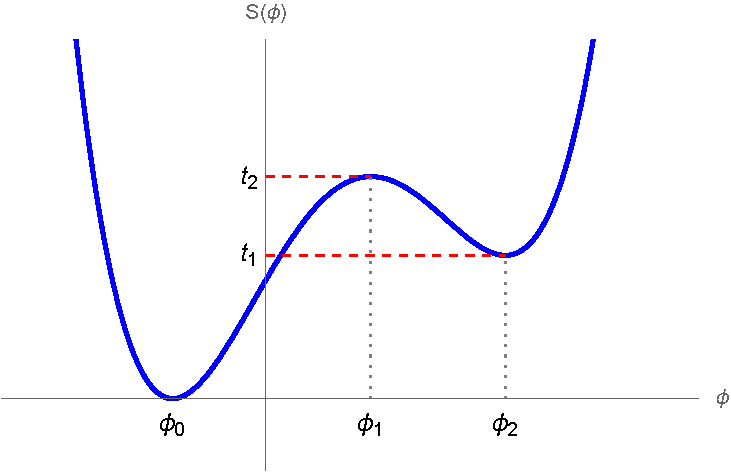
\includegraphics[width=.5\textwidth]{figures/borel1}}
%\caption{Borel. }
\label{fig:borelone}
\end{figure}


Returning to the setup of (\ref{zgintex}), we now consider the case where $S(\phi)$ has additional critical points, say at $\phi=\phi_i$ where $S'(\phi_i)=0$, $S(\phi_i)=t_i>0$, $i=1,2$. While (\ref{zgftrel}) still holds, $F(t)$ is no longer analytic at $t=t_i$, and therefore cannot be defined as the analytic continuation of the series (\ref{fttaylor}) to the entire positive real axis. Said differently, let $\widehat F(t)$ be the analytic continuation of the series on the RHS of (\ref{fttaylor}) from its domain of convergence $|t|<R$ to the complex $t$-plane, then $\widehat F(t)$ has branch points at $t=t_1$ and $t=t_2$, and does not agree with $F(t)$ defined in (\ref{zgftrel}) to the right of the branch points on the positive real axis.

One approach to recover $F(t)$ from $\widehat F(t)$ is as follows. One considers a deformation of (\ref{zgintex})
\ie\label{zgintexdeform}
Z_\theta(g) = \int_{\mathbb{R}} d\phi \,e^{-{1\over g} S_\theta(\phi)},~~~~ S_\theta(\phi) = e^{i\theta} S(\phi),
\fe
where $\theta$ is a small positive real number, so that $Z(g) = \lim_{\theta\to 0} Z_\theta(g)$. By assumption, $S_\theta(\phi)$ is still analytic on the entire complex $\phi$-plane, and so we can replace the real contour $\mathbb{R}$ with a homologous contour
\ie
C = \sum_i C_i,
\fe
where each $C_i$ is a steepest descent path $C_i^-$ followed by a steepest ascent path $C_i^+$ with respect to the height function ${\rm Re}(S_\theta(\phi))$, with $C_i^-$ and $C_i^+$ joining at the saddle point $\phi = \phi_i$. More explicitly, we may parameterize $C_i^\pm$ as $\phi = \phi(s)$, $s\in \mathbb{R}$, such that
\ie
{d\phi\over ds} = \pm {\partial\over \partial \phi^*} {\rm Re}(S_\theta(\phi)) = \pm {1\over 2} (S_\theta'(\phi))^*.
\fe
Along $C_i$, we have ${d\over ds}{\rm Im}(S_\theta(\phi))=0$ and $S_\theta(\phi) - S_\theta(\phi_i)$ is real and non-negative. We can thus decompose
\ie\label{zthetadecomp}
Z_\theta(g) = \sum_i Z_\theta^{(i)}(g),
~~~~ Z_\theta^{(i)}(g) = e^{-{1\over g} S_\theta(\phi_i)} \int_0^\infty dt\, e^{-{t\over g}} F_\theta^{(i)}(t),
\fe
where
\ie
F_\theta^{(i)}(t) \equiv \int_{C_i} d\phi \,\delta\left(t-(S_\theta(\phi) - S_\theta(\phi_i))\right)
\fe
can be recovered from the analytic continuation of the perturbative series for $Z_\theta(g)$ around $\phi=\phi_i$ by the same argument as in (\ref{zgftrel}), (\ref{fttaylor}). That is, each $Z_\theta^{(i)}(g)$ is given by the Borel resummation of the perturbative series around the saddle point $\phi=\phi_i$.

In particular, $F_\theta^{(0)}(t)$ associated with the ``perturbative saddle'' $\phi = \phi_0$ is related to the analytic continued Borel transformation $\widehat F(t)$ of the original perturbative series by $F_\theta^{(0)}(t) = e^{-i\theta} \widehat F(e^{-i\theta} t)$, and so we can write
\ie
\lim_{\theta\to 0^+} Z_\theta^{(0)}(g) = \lim_{\theta\to 0^+} \int_{e^{-i\theta} \mathbb{R}_+} dt\, e^{-{t\over g}} \widehat F(t).
\fe
In other words, $\lim_{\theta\to 0^+} Z_\theta^{(0)}(g)$ amounts to the inverse Borel transform of $\widehat F(t)$ defined with the $t$-integration contour $e^{-i\epsilon} \mathbb{R}_+$, evading the branch points at $t=t_1, t_2$. However, it must be supplemented with the ``instanton corrections'' $\lim_{\theta\to 0^+} Z_\theta^{(i)}(g)$, $i=1,2$, according to (\ref{zthetadecomp}), to recover $Z(g)$.


\subsection{Lefschetz thimbles}

The treatment of the previous section can be generalized to the multi-dimensional integral
\ie\label{zgmultiex}
Z(g) = \int_{\mathbb{R}^N} d^N\phi \, e^{-{1\over g} S(\phi)},
\fe
where $S(\phi)$ is assumed to be an analytic function over $\mathbb{C}^N$ with isolated critical points. Moreover, we assume that the Hessian of $S(\phi)$ at each critical point $\phi = \phi_i$ is non-degenerate. As such, the Hessian of the height function $h(\phi, \phi^*) \equiv {\rm Re} (S(\phi))$ at $\phi_i$ is a $2N\times 2N$ Hermitian matrix whose eigenvalues come in pairs that are equal in magnitude with opposite signs. It follows that $\phi_i$ lies at the intersection between a {\it stable submanifold} or a {\it Lefschetz thimble} $C_i \subset \mathbb{C}^N$, consisting of all steepest ascent paths with respect to $h(\phi, \phi^*)$ that begin at $\phi=\phi_i$, and an unstable submanifold or anti-thimble $C_i^\perp\subset \mathbb{C}^N$ consisting of all steepest descent paths that begin at $\phi=\phi_i$. Up to a small perturbation of $S(\phi)$ such as the phase rotation (\ref{zgintexdeform}), we may assume that each thimble or anti-thimble contains only a single critical point.

We can then deform the integration contour $\mathbb{R}^N\subset \mathbb{C}^N$ to a homologous contour
\ie
C = \sum_i n_i C_i,
\fe
where the coefficient $n_i$ is the intersection of $\mathbb{R}^N$ with $C_i^\perp$, as $\#(C_i\cap C_j^\perp) = \delta_{ij}$. It follows that
\ie
Z(g) = \sum_i Z^{(i)}(g),~~~ Z^{(i)}(g) = e^{-{1\over g} S(\phi_i)} \int_0^\infty dt \, e^{-{t\over g}} F^{(i)}(t),
\fe
where
\ie
F^{(i)}(t) \equiv \int_{C_i} d\phi \, \delta(t - (S(\phi) - S(\phi_i)))
\fe
is the Borel transformation of the perturbative series of (\ref{zgmultiex}) around $\phi=\phi_i$ similarly to (\ref{fttaylor}). The regularity of the thimble $C_i$ (which by assumption does not contain other critical points) ensures that $F^{(i)}(t)$ can be analytically continued to a neighborhood of the positive real $t$-axis. In other words, the perturbative series around $\phi=\phi_i$ is Borel summable, and $Z^{(i)}(g)$ is the result of Borel resummation.




\newpage

\section{Path integral quantization of gauge theories}

\subsection{The Faddeev-Popov ansatz}
\label{sec:fpderiv}

Let us denote by $\phi$ collectively the matter and gauge fields, and let $S[\phi]$ be an action that is invariant under the gauge transformation of the form 
\ie
\phi \mapsto \phi^\zeta \equiv f_\zeta(\phi), 
\fe
where $f_\zeta$ is a diffeomorphism on the space of fields labeled by a set of parameters $\zeta^\A$. We further assume that successive gauge transformations compose according to $(\phi^{\zeta_1})^{\zeta_2} = \phi^{\zeta_2\circ \zeta_1}$, where $\zeta_2\circ\zeta_1$ is independent of the field $\phi$. As such, $\zeta$ can be viewed as an element of a certain group of gauge transformations ${\cal G}$, with $\circ$ being the group multiplication. 

Formally the path integral takes the form
\ie\label{zpathapp}
Z = {1\over {\rm vol}({\cal G})} \int [D\phi] e^{i S[\phi]},
\fe
where ${\rm vol}({\cal G})$ will be defined more precisely in (\ref{volgdef}) below.
A gauge fixing condition of the form
\ie
F^A[\phi]=0
\fe
can be implemented by inserting
\ie
1 = \int_{\cal G} D\zeta\, \delta(F^A[\phi^\zeta]) \det {\partial F^A[\phi^\zeta] \over \partial \zeta^\A}
\fe
into the functional integral on the RHS of (\ref{zpathapp}), where $D\zeta = \prod_\A d\zeta^\A$ for an arbitrary coordinate system $\zeta^\A$ on ${\cal G}$. This leads to formally
\ie
\int [D\phi] e^{i S[\phi]} &= \int_{\cal G} D\zeta \int [D\phi] \, \delta(F^A[\phi^\zeta]) \det {\partial F^A[\phi^\zeta] \over \partial \zeta^\A} e^{i S[\phi]}
\\
&=  \int_{\cal G} D\zeta \int [D\phi] \, \delta(F^A[\phi]) \det {\partial F^A[\phi^{\zeta'\circ \zeta^{-1}}] \over \partial \zeta'^\A} \bigg|_{\zeta'=\zeta} e^{i S[\phi]},
\fe
where the second equality follows from the change of integration variable $\phi\to \phi' = \phi^{\zeta^{-1}}$, with $\zeta^{-1}$ labeling the inverse gauge transformation of $\zeta$. The integration over $\zeta$ yields a factor
\ie\label{zetahaar}
\int_{\cal G} D\zeta \,  \det {\partial F^A[\phi^{\zeta'\circ \zeta^{-1}}] \over \partial \zeta'^\A} \bigg|_{\zeta'=\zeta} = \int_{\cal G} D\zeta \, \left( \det {\partial (\zeta''\circ \zeta)^\A \over \partial \zeta''^\B} \right)^{-1} \bigg|_{\zeta''={\rm id}}  \det {\partial F^A[\phi^{\zeta''}] \over \partial \zeta''^\A} \bigg|_{\zeta''={\rm id}},
\fe
where we have written $\zeta' = \zeta''\circ \zeta$ and applied the chain rule of derivation. On the RHS, the first factor in the integrand combines with the measure to give
\ie
[D\zeta]_H \equiv D\zeta \, \left( \det {\partial (\zeta''\circ \zeta)^\A \over \partial \zeta''^\B} \right)^{-1} \bigg|_{\zeta''={\rm id}} ,
\fe
which is none other than the Haar measure on ${\cal G}$. In particular, it obeys the invariance property $[D(\zeta\circ \zeta_1)]_H = [D\zeta]_H$ for any fixed element $\zeta_1$ of ${\cal G}$. After dividing by the volume of the gauge group 
\ie\label{volgdef}
{\rm vol}({\cal G}) = \int_{\cal G} [D\zeta]_H
\fe
as in (\ref{zpathapp}), we are left with the gauge-fixed form of the path integral (\ref{zfix}) where the Faddeev-Popov determinant arises from the last factor on the RHS of (\ref{zetahaar}).


\subsection{Batalin-Vilkovisky quantization of gauge theory}
\label{app:bvgauge}

Now let us consider an action $S[\phi]$ that is invariant under infinitesimal gauge transformations of the general form
\ie
\delta \phi^i = \zeta^\A f_\A^i[\phi].
\fe
%Further, suppose that the commutator of a pair of gauge transformations takes the form
%\ie{}
%[\delta_\A, \delta_\B] \phi^i
%&= f^j_\A[\phi] {\delta f_\B^i[\phi]\over \delta\phi^j} - (\A\leftrightarrow\B) = f_{\A\B}{}^\C[\phi] f_\C^i[\phi].
%\fe
As in (\ref{gaugevar}) our notation is such that the repeated index $\A$ comes with integration with respect to a suitable measure on $\A$-space. For simplicity of discussion we will assume that both $\phi^i$ and $\zeta^\A$ are Grassmann-even. Similar to the BRST quantization prescription of section \ref{sec:brstinit}, we will associate a Grassmann-odd ghost field $c^\A$ with the gauge parameter $\zeta^\A$. We will further introduce a Grassmann-odd ``anti-field" $\phi^\ddagger_i$ that is paired with $\phi^i$, as well as a Grassmann-even ``anti-ghost" field $c^\ddagger_\A$ that is paired with the ghost field $c^\A$. We will assign ghost number 1 to $c^\A$, 0 to $\phi^i$, $-1$ to $\phi^\ddagger_i$ and $-2$ to $c^\ddagger_\A$. The BV action is a functional ${\mathbb S}[\phi, c, \phi^\ddagger, c^\ddagger]$ of ghost number zero, whose expansion in the Grassmann-odd ghost and anti-fields takes the form
\ie\label{bvexp}
&{\mathbb S}[\phi, c, \phi^\ddagger, c^\ddagger] 
\\
&= S[\phi] + c^\A f_\A^i[\phi] \phi^\ddagger_i + {1\over 2} c^\A c^\B f_{\A\B}{}^\C[\phi] c_\C^\ddagger + {1\over 4} c^\A c^\B f_{\A\B}{}^{ij}[\phi] \phi^\ddagger_i \phi^\ddagger_j + {1\over 6} c^\A c^\B c^\C f_{\A\B\C}{}^{i \D} [\phi] \phi^\ddagger_i c^\ddagger_\D + \cdots .
\fe
In particular, the first term on the RHS is the original action $S[\phi]$ and the second term $c^\A f_\A^i[\phi] \phi_i^\ddagger$ involves the gauge variation $\delta_\A\phi^i \equiv f_\A^i[\phi]$.

The quantum BV master equation (\ref{ssbvmast}) can be expressed as
\ie\label{clasbvgausimp}
{\delta_R \mathbb{S}\over \delta \phi_i^\ddagger} {\delta \mathbb{S}\over \delta \phi^i} + {\delta_R \mathbb{S}\over \delta c^\ddagger_\A} {\delta \mathbb{S}\over \delta c^\A} = - \hbar {\delta_R \delta \mathbb{S}\over \delta \phi_i^\ddagger \delta \phi^i} - \hbar {\delta_R \delta \mathbb{S}\over \delta c^\ddagger_\A \delta c^\A} ,
\fe
where $\delta$ and $\delta_R$ stand for left and right derivatives, taking into account the appropriate statistics of the fields involved, and we have restored the factor of $\hbar$ on the RHS to emphasize the quantum origin of these terms. Plugging (\ref{bvexp}) into (\ref{clasbvgausimp}) then leads to a set of equations, organized according to increasing powers of the $c$ ghosts,
\ie\label{bvunpacked}
& c^\A f_\A^i[\phi]  {\delta S[\phi] \over \delta \phi^i} = - \hbar c^\A {\delta f^i_\A[\phi] \over \delta\phi^i} - \hbar c^\A f_{\B \A}{}^\B[\phi] ,
\\
& c^\A c^\B\phi_i^\ddagger\left\{  f_\A^j[\phi]  {\delta f_\B^i[\phi] \over \delta \phi^j} - f_\B^j[\phi]  {\delta f_\A^i[\phi] \over \delta \phi^j} + f_{\A\B}{}^\C[\phi] f_\C^i + f_{\A\B}{}^{ji}[\phi] {\delta S[\phi]\over \delta \phi_j} \right\} = {\cal O}(\hbar),
\\
& c^\A c^\B c^\C c^\ddagger_\D \left\{ 3 f_{[\A}^i {\delta f_{\B\C]}{}^\D\over \delta \phi^i} - 3 f_{[\A\B}{}^\sigma[\phi] f_{\C]\sigma}{}^\D[\phi] -  f_{\A\B\C}{}^{i\D} {\delta S[\phi]\over \delta\phi^i} \right\} = {\cal O}(\hbar),~~~~{\rm etc.}
\fe
The first equation of (\ref{bvunpacked}) simply asserts that the action $S[\phi]$ is gauge invariant up to a quantum correction that arise from the Jacobian of the gauge transformation. The second equation of (\ref{bvunpacked}) amounts to the statement that the gauge algebra closes {\it on-shell}, with possibly-field-dependent structure constants $-f_{\A\B}{}^\C[\phi]$, up to quantum corrections. The third equation of (\ref{bvunpacked}) asserts that the generalized Jacobi-identity for the field-dependent structure constants hold on-shell up to quantum corrections, and so forth. 

When the gauge algebra closes off-shell with field-independent structure constants $-f_{\A\B}{}^\C$, the BRST formalism is recovered by treating $\phi^i$ as well as the Lagrange multiplier $B_A$ as matter fields, $c^\A$ and $b_A$ as ghost fields, together with the anti-fields $\phi_i^\ddagger, B^{\ddagger A}, c_\A^\ddagger, b^{\ddagger A}$, governed by the BV action functional
\ie\label{bvsimp}
\mathbb{S}[\phi, c, b, B, \phi^\ddagger, c^\ddagger, b^\ddagger, B^\ddagger] = S[\phi] + c^\A f^i_\A[\phi] \phi_i^\ddagger + i B_A b^{\ddagger A}  + {1\over 2} f_{\A\B}{}^\C c^\A c^\B c_\C^\ddagger.
\fe
Note that $B^{\ddagger A}$ is absent on the RHS. Applying the BV gauge condition (\ref{bvfix}) with
\ie
V= - b_A F^A[\phi]
\fe
then sets
\ie
\phi_i^\ddagger = - b_A {\delta F^A[\phi] \over \delta\phi^i},~~~ b^{\ddagger A} = - F^A[\phi],~~~ c^\ddagger_\A=0.
\fe
Plugging this back into (\ref{bvsimp}), we recover the standard gauge fixed BRST invariant action appearing in (\ref{bfix}).

A salient feature of the BV formulation of quantum gauge theory is that the quantum BV master equation can be preserved at the level of the Wilsonian effective action, as follows. Starting with the gauge-fixed path integral (\ref{gaugefixedbvpath}), we split the fields and anti-fields into low momentum modes $(\Phi_<, \Phi^\ddagger_<)$ and high momentum modes $(\Phi_>, \Phi_>^\ddagger)$, and consider $S_{\rm eff}[\Phi_<, \Phi_<^\ddagger]$ defined by
\ie
e^{-S_{\rm eff}[\Phi_<, \Phi_<^\ddagger]} = \int_{L_{V_>}} d\Phi_> e^{- S [\Phi_<, \Phi_<^\ddagger; \Phi_>, \Phi_>^\ddagger]}.
\fe
Here $L_{V_>}$ is the field-subspace defined by
\ie
L_{V_>}: \Phi_{I>}^\ddagger = {\delta V_>[\Phi_>]\over \delta \Phi^{I}_>}
\fe
for some Grassmann-odd functional $V_>[\Phi_>]$. Using the quantum BV master equation (\ref{qbvmastabs}) satisfied by the bare action $S [\Phi_<, \Phi_<^\ddagger; \Phi_>, \Phi_>^\ddagger]$, and performing an integration by part similarly to the manipulation of (\ref{zvvars}), we have
\ie{} 
{\delta_R \over \delta\Phi_{I<}^\ddagger}{\delta\over \delta\Phi_<^I} e^{-S_{\rm eff}[\Phi_<,\Phi_<^\ddagger]}
&=  \int_{L_{V_>}} d\Phi_>  {\delta_R \over \delta\Phi_{I<}^\ddagger}{\delta\over \delta\Phi_<^I}  e^{- S[\Phi_<, \Phi_<^\ddagger; \Phi_>, \Phi_>^\ddagger]} 
\\
&= - \int_{L_{V_>}} d\Phi_>   {\delta_R \over \delta\Phi_{I>}^\ddagger}{\delta\over \delta\Phi_>^I}  e^{- S[\Phi_<, \Phi_<^\ddagger; \Phi_>, \Phi_>^\ddagger]}
\\
&= %- \int d\Phi_>  {\delta\over \delta\Phi_>^I} \left(  {\delta_R \over \delta\Phi_{I>}^\ddagger}  e^{- S[\Phi_<, \Phi_<^\ddagger; \Phi_>, \Phi_>^\ddagger]} \bigg|_{\Phi_>^\ddagger= {\delta V_>\over \delta\Phi_>}} \right) 
\int_{L_{V_>}} d\Phi_> {\delta^2 V_>\over \delta \Phi_>^I \delta \Phi_>^J} {\delta\over \delta\Phi_{J>}^\ddagger}  {\delta_R \over \delta\Phi_{I>}^\ddagger}  e^{- S[\Phi_<, \Phi_<^\ddagger; \Phi_>, \Phi_>^\ddagger]} = 0 ,
\fe
which shows that $S_{\rm eff}[\Phi_<, \Phi_<^\ddagger]$ obeys the quantum BV master equation with respect to the low momentum modes of the fields and anti-fields. Upon imposing gauge condition on the low momentum modes, $S_{\rm eff}[\Phi_<, \Phi_<^\ddagger]$ then gives rise to a consistent Wilsonian path integral.


\newpage


\section{Local quantum field theories}

\subsection{Field operators}


We begin by considering a Poincar\'e invariant quantum field theory in $d$-dimensional Minkowskian spacetime, parameterized by the coordinates $x^0,\cdots, x^{d-1}$. The Poincar\'e symmetry associated with the spacetime coordinate transformation
\ie
x^\mu\mapsto x'^\mu = \Lambda^\mu{}_\nu x^\nu + a^\mu,
\fe
where $\Lambda^\mu{}_\nu$ obeys $\eta^{\rho\sigma} \Lambda^\mu{}_\rho \Lambda^\nu{}_\sigma = \eta^{\mu\nu}$, $\eta^{\mu\nu}$ being the Minkowskian metric in mostly plus signature convention $\eta^{\mu\nu} \equiv {\rm diag} \{-1, 1,\cdots,1\}$, is represented by a unitary operator $U(\Lambda, a)$ that obeys
\ie\label{ullamdu}
U(\Lambda', a') U(\Lambda, a) = U(\Lambda'\Lambda, \Lambda' a + a').
\fe
For infinitesimal transformation of the form
\ie\label{lamlorinfis}
\Lambda^\mu{}_\nu = \delta^\mu_\nu + \omega^\mu{}_\nu, ~~~~ a^\mu = \epsilon^\mu,
\fe
we can write at the first order with respect to $\omega^{\mu\nu} = -\omega^{\nu\mu}$ and $\epsilon^\mu$,
\ie\label{pjomer}
U(\Lambda, a) = 1 - i \epsilon^\mu \hat P_\mu + {i\over 2} \omega_{\mu\nu} \hat J^{\mu\nu}.
\fe
$\hat P^\mu$ is the momentum operator, with $\hat P^0 \equiv H$ being the Hamiltonian, and $\hat J^{\mu\nu}$ are the Lorentz boost and angular momentum operators. They obey the commutation relations
\ie\label{poincalgcomm}
& [\hat P^\mu, \hat J^{\rho\sigma}] = -i \left(\eta^{\mu\rho} \hat P^\sigma - \eta^{\mu\sigma} \hat P^\rho \right),
\\
& [\hat J^{\mu\nu}, \hat J^{\rho\sigma}] = -i \left( \eta^{\nu\rho} \hat J^{\mu\sigma} - \eta^{\mu\rho} \hat J^{\nu\sigma} - \eta^{\nu\sigma} \hat J^{\mu\rho} + \eta^{\mu\sigma} \hat J^{\nu\rho} \right).
\fe

A local field operator $\hat\Phi_\A(x)$ obeys the Poincar\'e transformation property
\ie\label{phiuutrans}
U(\Lambda, a) \hat\Phi_\A(x) (U(\Lambda, a))^{-1} = (R(\Lambda))_\A{}^\B\hat\Phi_\B(\Lambda x + a),
\fe
where $R(\Lambda)$ is a representation matrix of the Lorentz group that obeys $R(\Lambda_1\Lambda_2) = R(\Lambda_2) R(\Lambda_1)$.\footnote{Note that the composition rule of $R$ is in the opposite order compared to that of $U$ in (\ref{ullamdu}). In particular, associated with (\ref{lamlorinfis}) we can write $R(\Lambda) = \exp(- {i\over 2} \omega_{\mu\nu} S^{\mu\nu})$, where $S^{\mu\nu}$ are constant matrices that obey the same commutation relations among themselves as the operators $\hat J^{\mu\nu}$ in (\ref{poincalgcomm}). The example of the spinor representation is given by (\ref{spinorlorenzgen}), (\ref{spinorlorecomm}).} Further, the microcausality property asserts that any pair of local field operators $\hat\Phi(x)$ and $\hat\Phi'(y)$ obey
\ie\label{microcaus}
\big[ \hat\Phi(x), \hat\Phi'(y) \big] = 0 ~~~{\rm if}~~(x-y)^2\equiv (\vec x-\vec y)^2 - (x^0-y^0)^2  > 0.
\fe
A special local operator is the stress-energy tensor $T_{\mu\nu}(x)$, which obeys the symmetry and conservation law
\ie\label{trancurr}
T_{\mu\nu}(x) = T_{\nu\mu}(x), ~~~~ \partial_\mu T^\mu{}_{\nu}(x) = 0.
\fe
Moreover, the Poincar\'e generators $\hat P_\mu$ and $\hat J^{\mu\nu}$ are Noether charges associated with conserved currents built out of the stress-energy tensor,
\ie\label{patcab}
& \hat P^\mu = \int d^{d-1} \vec x T^{0\mu}(x) ,
\\
& \hat J^{\mu\nu} = \int d^{d-1} \vec x \left[ x^\mu T^{0\nu}(x) - x^\nu T^{0\mu}(x)  \right].
\fe

%It also follows from (\ref{trancurr}) that
%\ie\label{momcurr}
%\partial_a (x^b T^{ac} - x^c T^{ab}) = 0,
%\fe
%and the conserved charges associated with the current $J^{bc}_a \equiv x^b T_a{}^c - x^c T_a{}^b$ are the angular momentum and Lorentz boost charges $J^{bc}$. 



\subsection{Correlation functions}
\label{corrsec}


Assuming that there is a Poincar\'e invariant vacuum state $|0\rangle$, the Wightman function\footnote{Strictly speaking, the Wightman function (\ref{corrfngen}) should be viewed as a tempered distribution. See Streater and Wightman,
{\it PCT, spin and statistics, and all that} \cite{Streater:1989vi}; Glimm and Jaffe,
{\it Quantum Physics. A Functional Integral Point of View} \cite{Glimm:1987ng}.} of local field operators ${\cal O}_1, \cdots, {\cal O}_n$ is defined as the vacuum expectation value
\ie\label{corrfngen}
%\left\langle {\cal O}_1(x_1)\cdots {\cal O}_n(x_n) \right\rangle \equiv 
\langle 0| {\cal O}_1(x_1)\cdots {\cal O}_n(x_n) |0\rangle.
\fe
%We will also assume microcausality, meaning that any pair of local (bosonic) operators ${\cal O}_i(x)$ and ${\cal O}_j(y)$ at spacetime points $x=(x^0, \vec x)$, $y=(y^0, \vec y)$ commute provided that $x$ and $y$ are spacelike separated, namely
%\ie{}
%[{\cal O}_i(x) , {\cal O}_j(y)] = 0,~~~(x-y)^2 \equiv (\vec x-\vec y)^2 - (x^0-y^0)^2 > 0.
%\fe
It follows from microcausality (\ref{microcaus}) that if all of the $x_i$'s appearing in (\ref{corrfngen}) are spacelike separated, then the correlation function is independent of the ordering of the operators. Starting from such a configuration, we can analytically continue the time coordinates $x_i^0$'s to imaginary values $- i \tau_i$, and obtain the Euclidean correlation function (also known as Schwinger function)
\ie\label{euccorr}
\left\langle {\cal O}_1(x_1^E)\cdots {\cal O}_n(x_n^E) \right\rangle,~~~ x_i^E\equiv (\vec x_i, \tau_i) \in \mathbb{R}^d,
\fe
provided that
\ie
\tau_1 > \tau_2 > \cdots > \tau_n.
\fe
Such an analytic continuation is possible because we can write (\ref{corrfngen}) equivalently as
\ie{}
%\left\langle 0| {\cal O}_1(x_1)\cdots {\cal O}_n(x_n) |0 \right\rangle 
& \int d\A_1 \cdots d\A_{n-1} \langle 0| {\cal O}_1(x_1)|\A_1\rangle  \langle\A_1| {\cal O}_2(x_2) \cdots {\cal O}_{n-1}(x_{n-1}) |\A_{n-1}\rangle \langle \A_{n-1}| {\cal O}_n(x_n)|0\rangle
\\
&=  \int d\A_1 \cdots d\A_{n-1}  \langle 0| {\cal O}(0)|\A_1\rangle e^{iP_{\A_1}\cdot (x_1-x_2)} \langle\A_1| \cdots |\A_{n-1}\rangle e^{i P_{\A_{n-1}} \cdot (x_{n-1}-x_n)} \langle \A_{n-1}| {\cal O}_n(0)|0\rangle
\fe
where each $\{|\A_i\rangle\}$ is a complete basis of the Hilbert space consisting of eigenstates with energy-momentum vector $P_{\A_i}=(E_{\A_i}, \vec P_{\A_i})$, and normalized such that $\int d\A_i |\A_i\rangle \langle\A_i|=1$. Given that the energy $E_\A$ is bounded from below, the sum over states is expected to be absolutely convergent for ${\rm Im}(x_i^0-x_{i+1}^0) < 0$, leading to an analytic function of $x_i^0$.


\begin{figure}[h!]
\centering
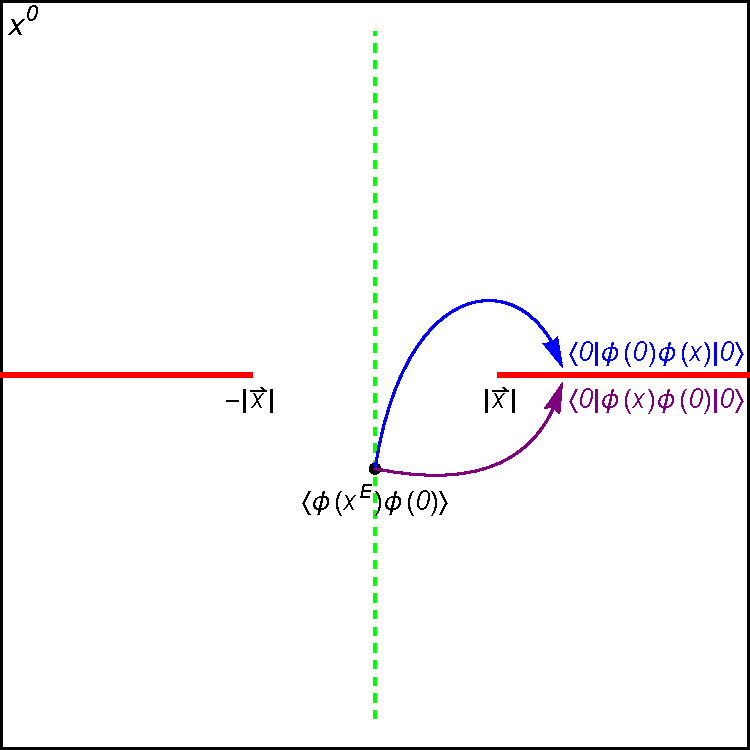
\includegraphics[width=.4\textwidth]{figures/greenanalytic.pdf}
\caption{The complex $x^0$-plane, with the imaginary $x^0$-axis (negative Euclidean time) indicated by the dashed green vertical line. The Wightman functions $\langle 0|\phi(x) \phi(0)|0\rangle$ and $\langle 0|\phi(0) \phi(x) |0\rangle$ are obtained as the analytic continuations of the Euclidean 2-point function $\langle \phi(x^E)\phi(0)\rangle$ above and below the branch cuts $x^0 \in (-\infty, -|\vec x|] \cup [|\vec x|,\infty)$ respectively. }\label{fig:greenanalytic}
\end{figure}

If the $x_i$'s are spacelike separated to begin with, it follows from the microcausality (\ref{microcaus}) that the ordering of ${\cal O}_i(x_i)$'s does not affect the value of the Wightman function. Moreover, the Wightman function is analytic in this domain. A closely related property is that the Euclidean correlation function (\ref{euccorr}) is a real analytic function in the $x_i^E$'s provided that the latter are separated points in $\mathbb{R}^d$. Starting from the Euclidean correlation function, we can also go back to the Lorentzian Wightman function by analytic continuation in $\tau_i$. We expect singularities when a pair of points $x_i$ and $x_j$ become null-separated, and therefore the analytic continuation must be performed in a way that avoids the singularities, e.g. by maintaining the condition ${\rm Im}(x_i^0-x_j^0)<0$ in the vicinity of the Lorentzian kinematic region. In particular, we can approach the Lorentzian configuration while maintaining the separation of the points in imaginary (or Euclidean) time and nonzero $(x_i-x_j)^2 = (\vec x_i -\vec x_j)^2-(x_i^0-x_j^0)^2$. If $x_i$ and $x_j$ are to become timelike separated, i.e. $(x_i-x_j)^2$ goes from a positive real value to a negative real value, the operator ordering between ${\cal O}_i$ and ${\cal O}_j$ in the resulting Lorentzian correlator is specified by whether $(x_i-x_j)^2$ goes around zero from above or below the real axis in the analytic continuation procedure (Figure \ref{fig:greenanalytic}).


\subsection{Conformal symmetry}

The trace of the stress-energy tensor, $T^a{}_a$, is a scalar operator. Typically, one expresses it as a linear combination of a basis of scalar operators ${\cal O}_I$,
\ie
T^a{}_a = \sum_I \beta_I {\cal O}_I,
\fe
where the coefficients $\beta_I$ are known as beta functions.

A conformal field theory (CFT) is a quantum field theory whose stress-energy tensor $T_{ab}$ is traceless, namely
\ie\label{tracelesst}
T^a{}_a = 0.
\fe
It follows from (\ref{tracelesst}) that there are new conservation laws
\ie\label{confcurr}
\partial_a( x^b T^a{}_b)=0,~~~ \partial_a (T^{ab} x^2 - 2 T^a{}_c x^b x^c ) = 0.
\fe
The symmetries generated by a conserved current of the form $J_a(x) = T_{ab}(x) v^b(x)$ obey the same algebra as those of the vector fields $v^a(x) \partial_a$, which generate the infinitesimal diffeomorphism
\ie
x^a \mapsto x'^a = x^a + \epsilon v^a(x).
\fe
In this sense, we can organize the symmetries generated by the conserved currents appearing in (\ref{trancurr}), (\ref{patcab}), (\ref{confcurr}) according to the diffeomorphisms generated by the vector fields
\ie\label{dvecf}
\partial_a,~~~ x_a \partial_b - x_b \partial_a,~~~ x^a \partial_a,~~~ x^2 \partial_a - 2 x_a x^b \partial_b.
\fe
(\ref{dvecf}) generate the $d$-dimensional conformal group, which is isomorphic to $SO(d,2)$ for conformal symmetry in $d$-dimensional Minkowskian spacetime, or $SO(d+1,1)$ for conformal symmetry in Euclidean spacetime.


\subsection{Operator product expansion}
\label{opesec}

In the Euclidean signature, rather than working with constant time slices, we may consider any $(d-1)$-dimensional oriented hypersurface ${\cal S}$ in $\mathbb{R}^d$, and consider a suitable space $V_{\cal S}$ of states on ${\cal S}$. In a path integral formulation, such states may be specified by wave functionals on ${\cal S}$. Generally, there isn't a natural inner product defined on $V_{\cal S}$, and so $V_{\cal S}$ is not quite a Hilbert space (unless ${\cal S}$ is time-reflection symmetric).\footnote{For a more rigorous treatment see Kontsevich and Segal, Quart. J. Math. Oxford Ser. \textbf{72} (2021) no.1-2, 673 \cite{Kontsevich:2021dmb}.} Rather, we have a bilinear pairing between states in $V_{\cal S}$ and those in $V_{\overline{\cal S}}$, where $\overline{\cal S}$ is ${\cal S}$ with the opposite orientation. 

In a conformal field theory, however, if we take ${\cal S}$ to be a $(d-1)$-dimensional sphere centered at the origin, the inversion map gives rise to a natural isomorphism between $V_{\cal S}$ and $V_{\overline{\cal S}}$ (known as BPZ conjugation), and thereby an inner product on $V_{\cal S}$. Such an inner product is positive definite if the conformal field theory is unitary or equivalently reflection-positive. A class of states in $V_{\cal S}$ can be constructed as the wave functionals produced by the path integral on the ball ${\cal B}$ enclosed by ${\cal S}$, with a set of local operators ${\cal O}_i(x_i)$ inserted within ${\cal B}$; such a state will be denoted by 
\ie
| \textstyle\prod_i {\cal O}_i(x_i)\rangle_{\cal S}.
\fe
The completion of $V_{\cal S}$ with respect to its inner product, denoted by ${\cal H}_{\cal S}$, will be referred to as the Hilbert space associated with ${\cal S}$. The Noether charge associated with dilatation symmetry,
\ie
\widehat H = - \int_{{\cal S}} d\sigma \, n^\mu x^\nu T_{\mu\nu}(x) ,
\fe
where $d\sigma$ is the volume element of ${\cal S}$ and $\vec n^\mu$ is the unit normal vector pointing outward, can be identified as the Hamiltonian operator on ${\cal H}_S$.\footnote{$\widehat H$ agrees with the Hamiltonian on the cylinder $\mathbb{R}\times S^{d-1}$ up to a Casimir energy.} In particular, $\widehat H$ is Hermitian and typically has discrete spectrum,\footnote{Exceptions include 2D conformal nonlinear sigma models with noncompact target space, where the eigenstates with respect to $\widehat H$ may be delta-function normalizable.} in which case the eigenstates of $\widehat H$ form a complete basis of ${\cal H}_S$.

Any state $|\psi\rangle$ in ${\cal H}_S$ can be viewed as the state created by a certain, a priori non-local, operator supported in ${\cal B}$. Upon a dilatation symmetry transformation, $e^{-\widehat H \tau} |\psi\rangle$ is created by an operator supported in a ball whose radius is $e^{-\tau}$ times that of ${\cal B}$. When $|\psi\rangle$ is an eigenstate of $\widehat H$, we can take $\tau$ to be arbitrarily large and conclude that $|\psi\rangle$ is in fact created by a local operator supported at the origin. Moreover, the corresponding local operator has definite scaling dimension.
%Let $V_\varepsilon$ be the space of states in $V_{\cal S}$ created by a set of local operators in a small ball $B_\varepsilon(0)$ of radius $\varepsilon$ centered at the origin. We will now argue that $V_\varepsilon$ is in fact dense in ${\cal H}_{\cal S}$. Let $|\Phi_\A\rangle$ be an orthonormal basis of $V_\varepsilon$. Given any state $|\psi\rangle\in {\cal H}_{\cal S}$, let
%\ie
%|\psi'\rangle \equiv |\psi\rangle - \sum_{\A} \langle \Phi_\A|\psi\rangle |\Phi_\A\rangle
%\fe
%be the orthogonal projection of $|\psi\rangle$ onto $V_\varepsilon^\perp$. By construction, $|\psi'\rangle$ has vanishing pairing with all states in $V_{\overline{\cal S}}$ created by local operators related by inversion map to those in $B_\varepsilon(0)$; the latter local operators lie in the complement of $B_{\varepsilon^{-1}}(0)$. In other words, $|\psi\rangle$ has vanishing correlator with any set of local operators in the complement of $B_{\varepsilon^{-1}}(0)$. By analytic continuation of correlators, it follows that $|\psi'\rangle$ has vanishing pairing with all states in $V_{\overline {\cal S}}$ and therefore must be the zero state vector. This shows that the closure of $V_\varepsilon$ is in fact all of ${\cal H}_{\cal S}$.
%The space of local operators at the origin may be identified with the inverse limit $V_0 \equiv \lim\limits_{\longleftarrow}V_\varepsilon$ with respect to the natural inclusion $V_\varepsilon\hookrightarrow V_{\varepsilon'}$ for $\varepsilon<\varepsilon'$, over all positive $\varepsilon$.
It follows that the set of states $|{\cal O}_i(0)\rangle_{\cal S}$ created by local operators ${\cal O}_i$ of definite scaling dimension at the origin form a complete basis of ${\cal H}_{\cal S}$.

Given a pair of local operators ${\cal O}_i(x_i)$ and ${\cal O}_j(x_j)$ inside ${\cal B}$, the state $|{\cal O}_i(x_i) {\cal O}_j(x_j)\rangle_{\cal S}$ can be expanded in the aforementioned basis of ${\cal H}_S$ as
\ie\label{opegena}
|{\cal O}_i(x_i) {\cal O}_j(x_j)\rangle_{\cal S} = \sum_k C_{ij}^k(x_i, x_j) |{\cal O}_k(0)\rangle_{\cal S},
\fe
where $C_{ij}^k(x_i,x_j)$ are real analytic functions in $x_i$ and $x_j$, away from the locus $x_i=x_j$. This is known as the operator product expansion (OPE). 
(\ref{opegena}) can be viewed as an operator equation
\ie\label{opegen}
{\cal O}_i(x_i) {\cal O}_j(x_j) = \sum_k C_{ij}^k(x_i, x_j) {\cal O}_k(0),
\fe
in the sense that (\ref{opegen}) is expected to hold when inserted into a (Euclidean) correlation function, with a convergent sum over correlators involving ${\cal O}_k$ on the RHS, provided that all other local operators in the correlation function lie outside of ${\cal B}$.

We can of course also shift the origin of the ball ${\cal B}$, and write the OPE of a pair of operators around any given point $y\in\mathbb{R}^d$,
\ie
{\cal O}_i(x_i) {\cal O}_j(x_j) = \sum_k C_{ij}^k(x_i-y, x_j-y) {\cal O}_k(y),
\fe
provided that the minimal sphere centered at $y$ that encloses $x_i$ and $x_j$ does not enclose other local operators in a given correlation function. 

For further elaborations on the convergence property of OPEs and related analyticity properties of correlation functions in a conformal field theory, see Pappadopulo et al., Phys. Rev. D \textbf{86} (2012), 105043 \cite{Pappadopulo:2012jk}, and Kravchuk, Qiao and Rychkov, JHEP \textbf{05} (2020), 137 \cite{Kravchuk:2020scc}, JHEP \textbf{08} (2021), 094 \cite{Kravchuk:2021kwe}.







\newpage

\section{General properties of 2D CFTs}

%The Polyakov formalism of string theory is based on a dynamical metric coupled to a Weyl invariant field theory on the two dimensional worldsheet. Upon gauge fixing, the worldsheet theory can be described as a conformal field theory on a Riemann surface with zero central charge and a BRST symmetry. In this Appendix we introduce the defining properties and basic examples of 2D conformal field theories that serve as building blocks for the worldsheet theory.



\subsection{2D conventions}

In 2D Lorentzian signature, we typically denote by $\sigma$ the spatial coordinate and $t$ the time coordinate, and define the lightcone coordinates as $\sigma^\pm \equiv \sigma \pm t$. The Wick rotation to Euclidean signature is defined by $t = - i \tau$. We define the complex coordinates $(z, \bar z)$ as 
\ie
z = \sigma + i \tau,~~~~\bar z = \sigma - i \tau.
\fe
In other words, the Wick rotation takes $(\sigma^-, \sigma^+)$ to $(z, \bar z)$. Our convention for the measure in complex coordinate $z$ is such that 
\ie\label{dsqzconv}
d^2z \equiv 2 d{\rm Re}(z) d{\rm Im}(z). 
\fe
In the notation of differential forms, the integration measure $dz^2$ is equivalent to $i dz\wedge d\bar z$. The conventions for 2D spinors will be stated in Appendix \ref{freeferm}.

\subsection{2D conformal symmetry}

In two-dimensional spacetime, the conformal group is automatically enhanced to an infinite dimensional one. This is most easily seen by working in lightcone coordinates $(\sigma^-, \sigma^+)$, in which the traceless stress-energy tensor obeys
\ie
\partial_- T_{++} = \partial_+ T_{--} = 0,~~~~ T_{+-}=T_{-+}=0.
\fe
Consequently, we have an infinite set of conservation laws
\ie\label{confcurrents}
 \partial_+ ( v(\sigma^-) T_{--}) = 0,~~~~ \partial_- (\wt v(\sigma^+) T_{++}) = 0,
\fe
for any functions $v(\sigma^-)$ and $\widetilde v(\sigma^+)$. In Euclidean signature, $(\sigma^-, \sigma^+)$ are replaced by complex coordinates $(z,\bar z)$. The non-vanishing components of the stress-energy tensor are
\ie
T(z) \equiv T_{zz}(z),~~~~ \widetilde T(\bar z) \equiv T_{\bar z\bar z}(\bar z),
\fe
where we have indicated the conservation laws by declaring that $T(z)$ is holomorphic and $\widetilde T(\bar z)$ is anti-holomorphic. 

Let us note that the holomorphy of $T(z)$, like the conservation equations for any symmetry currents in a quantum field theory, should be understood as an operator equation, in the sense that any correlation function of local operators that involve $\bar\partial T$ vanishes,
\ie
\left\langle \bar\partial T(z) {\cal O}_1(z_1,\bar z_1)\cdots {\cal O}_n(z_n,\bar z_n) \right\rangle = 0,
\fe
provided that the points $z_1,\cdots, z_n$ are separated from $z$. This means that the correlation function
\ie\label{corrtos}
\left\langle T(z) {\cal O}_1(z_1,\bar z_1)\cdots {\cal O}_n(z_n,\bar z_n) \right\rangle 
\fe
is a holomorphic function in $z$, away from $z_1,\cdots, z_n$. Generally, (\ref{corrtos}) will have singularities when $z$ coincides with one of the $z_i$'s.


As a simple example, a linear conformal transformation amounts to a combination of translation, rotation, and dilation, which may be characterized by the linear holomorphic diffeomorphism
\ie\label{rescz}
z\mapsto z'= \lambda z + u,~~~\bar z \mapsto \bar z'= \bar\lambda \bar z + \bar u,
\fe
where $\lambda, u$ are complex constants, with $\lambda$ nonzero. If we set $u=0$, then (\ref{rescz}) would fix the origin, and the associated dilation/rotation maps an operator at the origin, ${\cal O}(0)$, to another operator at the origin ${\cal O}'(0)$. Typically, it is possible to find a basis of operators ${\cal O}$ on which dilation and rotation act diagonally, namely
\ie
{\cal O}'(0) = \lambda^{-h} \bar\lambda^{-\widetilde h} {\cal O}(0),
\fe
for a pair of constants $h$ and $\widetilde h$. We will refer to $h$ and $\widetilde h$ as the holomorphic and anti-holomorphic (or left and right) conformal weights of ${\cal O}$. For nonzero $u$, the linear conformal transformation takes ${\cal O}$ to ${\cal O}'$, such that
\ie\label{linconft}
{\cal O}'(u) = \lambda^{-h} \bar\lambda^{-\widetilde h} {\cal O}(0)
\fe

There is a conformal transformation that maps the punctured complex plane $\mathbb{C}^\times = \mathbb{C}-\{0\}$ to the Euclidean cylinder, parameterized by $w=\sigma + i\tau$, $\sigma\sim \sigma + 2\pi$, via the holomorphic diffeomorphism
\ie\label{zwexp}
z = e^{-i w}.
\fe
Heuristically, we then expect that a CFT on the plane, possibly with a singularity at the origin, to be equivalent to the same CFT on the Euclidean cylinder. The singularity at the origin can be characterized by an insertion of a local operator on the plane. The Euclidean cylinder is related to the Lorentzian cylinder by analytic continuation in $\tau$, and characterizes time evolution of the CFT defined on a spatial circle.

This leads to the state/operator correspondence, that is, there is a canonical 1-1 correspondence between the space of local operators in a CFT at a given point (here taken to be the origin of the complex plane) to the space ${\cal H}$ of states of the CFT on a circle of unit radius. Given a local operator ${\cal O}(0)$, we will write the corresponding state as $|{\cal O}\rangle$. 

The dilation and rotation symmetry (\ref{rescz}) on the plane corresponds to time and space translation on the cylinder under the state/operator map. Thus, we expect that an operator ${\cal O}(0)$ of conformal weight $(h,\widetilde h)$ to map to a state $|{\cal O}\rangle$ on the cylinder with energy $h+\widetilde h$ and spatial momentum $h-\widetilde h$. We will see in section \ref{virasorosec} that this is correct up to a shift of the ground state energy-momentum that is fixed by the conformal symmetry.

We may equivalently think of the state $|{\cal O}\rangle$ as defined by a wave functional on the unit circle ${\cal S}: |z|=1$ in the plane, obtained by performing the path integral on the disc $|z|\leq 1$ with the insertion of ${\cal O}(0)$, as described in section \ref{opesec}. The conformal symmetry corresponding to the inversion map $z'=1/z$ gives a natural identification between ${\cal H}_{\cal S}$ and ${\cal H}_{\overline {\cal S}}$, known as BPZ conjugation, thereby defining a bilinear inner product on ${\cal H}_{\cal S}$. The Hermitian inner product on ${\cal H}_{\cal S}$ is related by a further complex conjugation on one of the two states in the bilinear pairing.

The operator product expansion in a CFT can be organized according to the conformal weights. Namely, given a basis of local operators ${\cal O}_i(z,\bar z)$ of weight $(h_i, \widetilde h_i)$, we can write the OPE as
\ie\label{opecftt}
{\cal O}_i(z,\bar z) {\cal O}_j(0) = \sum_k C_{ij}^k z^{h_k-h_i-h_j}\bar z^{\widetilde h_k - \widetilde h_i - \widetilde h_j} {\cal O}_k(0),
\fe
where $C_{ij}^k$ are constants. When inserted into a correlation function, the RHS of (\ref{opecftt}) as a power series in $z, \bar z$ is expected to have a radius of convergence at least $R$ if there are no other local operators within the disc centered at 0 of radius $R$. In writing (\ref{opecftt}) we have only made use of the dilation and rotation symmetry. We will see in section \ref{confblocksec} that the full conformal symmetry leads to a much more refined version of the OPE, with far stronger convergence properties.

The conserved currents appearing in (\ref{confcurrents}) can be written in the Euclidean signature as holomorphic and anti-holomorphic currents
\ie
j(z) = v(z) T(z),~~~\widetilde j(\bar z) = \widetilde v(\bar z) \widetilde T(\bar z).
\fe
They generate the infinitesimal conformal transformations that correspond to the infinitesimal holomorphic diffeomorphisms
\ie\label{infconf}
z\mapsto z'=z + \epsilon v(z),~~~\bar z \mapsto\bar z'=\bar z + \epsilon \bar v(\bar z),
\fe 
by acting on a local operator ${\cal O}(z,\bar z)$ with the conserved charge
\ie
\widehat Q =  - \oint_C \left[ {dw\over 2\pi i} j(w) - {d\bar w\over 2\pi i} \widetilde j(\bar w) \right],
\fe
where $C$ is a counterclockwise contour that encircles $z$. That is to say, the infinitesimal conformal transformation maps the operator ${\cal O}(z,\bar z)$ to
\ie{}
&{\cal O}'(z,\bar z) = {\cal O}(z,\bar z) + \delta{\cal O}(z,\bar z),
\\
&\delta{\cal O}(z,\bar z) = \epsilon \widehat Q {\cal O}(z,\bar z) = - \epsilon\oint_C \left[ {dw\over 2\pi i} v(w) T(w) - {d\bar w\over 2\pi i} \widetilde v(\bar w) \widetilde T(\bar w) \right] {\cal O}(z,\bar z).
\fe
The contour integral on the RHS can also be expressed in terms of the singular terms in the OPE of the stress-energy tensor with ${\cal O}$, namely
\ie\label{inftro}
\delta{\cal O}(z,\bar z) = - \epsilon \left[ {\rm Res}_{w\to z} v(w) T(w) {\cal O}(z,\bar z) + \overline{\rm Res}_{\bar w\to \bar z} \widetilde v(\bar w) \widetilde T(\bar w) {\cal O}(z,\bar z) \right]
\fe
If ${\cal O}$ transforms under an infinitesimal linear conformal transformation $v(w)=\A w + \B$, $\widetilde v(\bar w) = \bar \A \bar w + \bar \B$ with definite conformal weights $(h, \widetilde h)$, as in (\ref{linconft}), then we know that
\ie
\delta {\cal O}(z,\bar z) =  - \epsilon ( h \A + \widetilde h \bar \A + \B \partial + \bar\B \bar\partial) {\cal O}(z,\bar z).
\fe
It follows that the OPE of $T, \widetilde T$ with ${\cal O}$ must take the form (after a overall translation and relabeling of coordinates)
\ie\label{toope}
& T(z) {\cal O}(0) = \cdots + {h\over z^2} {\cal O}(0) + {1\over z} \partial {\cal O}(0) + \cdots,
\\
& \widetilde T(\bar z) {\cal O}(0) = \cdots + {\widetilde h\over \bar z^2} {\cal O}(0) + {1\over \bar z} \bar\partial {\cal O}(0) + \cdots.
\fe
On the RHS of the first line, the $\cdots$ to the left represents terms in the Laurent expansion in $z$ of higher order poles than ${1\over z^2}$, whereas the $\cdots$ to the right represents terms that are regular at $z=0$. The omitted terms in the second line are similar, with $z$ replaced by $\bar z$. To determine the transformation of ${\cal O}$ under a more general conformal transformation with nonlinear $v(z)$, $\widetilde v(\bar z)$, would require knowing the higher order pole terms in the OPE (\ref{toope}).

A finite conformal transformation can be characterized by a general holomorphic diffeomorphism %\footnote{One shall not confuse the conformal symmetry with diffeomorphism symmetry, however, as the latter characterizes a gravitational theory and is not a symmetry of the CFT.}
\ie\label{finconf}
z\mapsto z'=z'(z),~~~\bar z \mapsto\bar z'=\bar z'(\bar z).
\fe
Under such a symmetry, a local operator ${\cal O}$ should transform into another operator ${\cal O}'$, such that ${\cal O}'(z', \bar z')$ behaves like a local operator at position $z$. If (\ref{finconf}) is obtained by composing infinitely many infinitesimal transformations of the form (\ref{infconf}), then we can determine ${\cal O}'$ by composing the infinitesimal transformations (\ref{inftro}) on the operator ${\cal O}$.

A special class of operators, called conformal {\it primary} operators or simply {\it primaries}, obey OPEs with the stress-energy tensor of the form (\ref{toope}) without higher than second order poles in $z$ or $\bar z$, namely
\ie\label{toprim}
& T(z) \phi(0) =  {h\over z^2} \phi(0) + {1\over z} \partial \phi(0) + \cdots,
\\
& \widetilde T(\bar z) \phi(0) =  {\widetilde h\over \bar z^2} \phi(0) + {1\over \bar z} \bar\partial \phi(0) + \cdots.
\fe
Under a general infinitesimal conformal transformation (\ref{infconf}), $\phi$ transforms by
\ie\label{infphi}
\delta\phi = - \epsilon (h \partial v + v \partial + \widetilde h \bar\partial \widetilde v + \widetilde v\bar\partial )\phi.
\fe
The finite form of the conformal transformation $\phi \to \phi'$ under (\ref{finconf}) can be expressed as
\ie
\phi'(z',\bar z') = (\partial_z z')^{-h} (\bar\partial_{\bar z} \bar z')^{-\widetilde h} \phi(z,\bar z).
\fe 



\subsection{The Virasoro algebra}
\label{virasorosec}

In a 2D CFT, the OPE of the holomorphic stress-energy tensor $T(z)$ with itself generally takes the form
\ie\label{ttopes}
T(z) T(0) \sim {c\over 2z^4} + {2\over z^2} T(0) + {1\over z} \partial T(0),
\fe
where the constant $c$ is called the central charge, and terms on the RHS that are regular at $z=0$ are omitted. Note that the terms of order ${1\over z^2}$ and ${1\over z}$ are determined by the fact that $T$ has conformal weight $(2,0)$. There is an analogous OPE of the anti-holomorphic stress-energy tensor $\widetilde T(\bar z)$ that involves another central charge $\widetilde c$. We have already seen that the free boson CFT has $c=\widetilde c=1$, whereas the free fermion theory has $c=\widetilde c={1\over 2}$.

The appearance of the order ${1\over z^4}$ term on the RHS of (\ref{ttopes}) implies that $T(z)$ is not a conformal primary. Rather, it transforms under the infinitesimal conformal transformation (\ref{infconf}) according to
\ie\label{inftt}
\delta T = - \epsilon\left[ (2 \partial v + v \partial) T + {c\over 12} \partial^3 v \right].
\fe
The finite form of the transformation, with respect to (\ref{finconf}), turns out to be
\ie\label{finttr}
T'(z', \bar z') = (\partial_z z')^{-2} \left[ T(z,\bar z) - {c\over 12} \{z',z\}_S \right],
\fe
where $\{z',z\}_S$ is the Schwarzian derivative, defined as
\ie
\{z',z\}_S \equiv {2 (\partial_z^3 z')(\partial_z z') - 3 (\partial_z^2 z')^2\over 2(\partial_z z')^2}.
\fe
Under successive conformal transforms $z\to z'\to z''$, (\ref{finttr}) composes correctly thanks to the following property of the Schwarzian derivative,
\ie
\{ z'', z\}_S = (\partial_z z')^2 \{z'', z'\}_S + \{z', z\}_S.
\fe
One can then prove (\ref{finttr}) by noting that it reduces to (\ref{inftt}) under infinitesimal transformations.

Under the state/operator map $z=e^{-iw}$, the stress-energy tensor $T^{(w)}$ on the cylinder and $T^{(z)}$ on the plane are related by
\ie
T^{(w)}(w) = (\partial_w z)^2 T^{(z)}(z) + {c\over 24}.
\fe
In the presence of an operator ${\cal O}(0)$ at the origin, we will write the Laurent expansion of $T^{(z)}(z)$ as
\ie\label{modcyhol}
T^{(z)}(z) = \sum_{n\in\mathbb{Z}} {L_n\over z^{n+2}}.
\fe
Correspondingly, on the cylinder, we have
\ie\label{modcyhola}
T^{(w)}(w) = - \sum_{n\in\mathbb{Z}} e^{inw} L_n + {c\over 24}.
\fe
We can write similar expansions for the anti-holomorphic stress-energy tensor,
\ie
\widetilde T^{(z)}(\bar z) = \sum_{n\in\mathbb{Z}} {\widetilde L_n\over \bar z^{n+2}},~~~~ \widetilde T^{(w)}(\bar w) = - \sum_{n\in\mathbb{Z}} e^{-in\bar w} \widetilde L_n + {\widetilde c\over 24}.
\fe
The energy and momentum on the cylinder can be written as\footnote{Note that our normalization convention of the stress-energy tensor in a 2D CFT, which is standard in the literature, differs from that of the stress-energy tensor appearing in (\ref{patcab}) by a factor $-{1\over 2\pi}$.}
\ie{}
& H = - \int_0^{2\pi} {d\sigma\over 2\pi} (T^{(w)})^{tt} = - \int_0^{2\pi} {d\sigma\over 2\pi} \left[ T^{(w)}(w) + \widetilde T^{(w)}(\bar w) \right],
\\
& P = - \int_0^{2\pi} {d\sigma\over 2\pi} (T^{(w)})^{t\sigma} = - \int_0^{2\pi} {d\sigma\over 2\pi} \left[ T^{(w)}(w) - \widetilde T^{(w)}(\bar w) \right].
\fe
In the second equality on each line, we converted the Lorentzian expressions to Euclidean expressions. Our convention of the momentum $P$ is in the direction of decreasing $\sigma$. Using (\ref{modcyhol}) and (\ref{modcyhola}), we can express $H$ and $P$ in terms of the zeroth Fourier modes as
\ie\label{hpid}
H = L_0 + \widetilde L_0 - {c+\widetilde c\over 24},~~~ P = L_0 - \widetilde L_0 - {c-\widetilde c\over 24}.
\fe
For an operator ${\cal O}(0)$ of conformal weight $(h, \widetilde h)$, it follows from the OPE (\ref{toope}) that
\ie{}
& L_0 |{\cal O}\rangle = h |{\cal O}\rangle, ~~~L_{-1}|{\cal O}\rangle = |\partial{\cal O}\rangle,
\\
& \widetilde L_0 |{\cal O}\rangle = \widetilde h |{\cal O}\rangle, ~~~\widetilde L_{-1}|{\cal O}\rangle = |\bar\partial{\cal O}\rangle.
\fe
We see that $H$ and $P$ can be identified with the dilation generator $L_0 + \widetilde L_0$ and the rotation generator $L_0 - \widetilde L_0$ up to constant shifts; the latter, proportional to the central charges, are interpreted as Casimir energy-momentum.

Of particular significance is the algebra generated by $L_n$ and $\widetilde L_n$ with respect to Lie brackets. Acting on a generic state/operator ${\cal O}(0)$, we can write
\ie\label{lnmcc}
L_n L_m = \oint_{C_1} {dz_1\over 2\pi i}\oint_{C_2} {dz_2\over 2\pi i} z_1^{n+1} z_2^{m+1} T(z_1) T(z_2),
\fe
where $C_1$, $C_2$ are a pair of counterclockwise contours encircling the origin, with $C_1$ outside of $C_2$. $L_m L_n$ would be given by an expression identical to (\ref{lnmcc}) except that $C_1$ would be replaced by another counterclockwise contour $C_1'$ that lies within $C_2$. 

The commutator $[L_n, L_m]$ is thus computed by the integral analogous to (\ref{lnmcc}), except that $z_1$ is integrated over $C_1-C_1'$, that is the union of the contour $C_1$ and the orientation reversal of $C_1'$.
The contour $C_1-C_1'$ now encloses every point on $C_2$, and does not enclose the origin. Therefore, we can shrink $C_1-C_1'$ to a counterclockwise contour $C_{z_2}$ encircling $z_2$ without affecting the integral. This leads to
\ie\label{lnmderv}
[L_n, L_m] &= \oint_{C_2} {dz_2\over 2\pi i} \oint_{C_{z_2}} {dz_1\over 2\pi i} z_1^{n+1} z_2^{m+1} T(z_1) T(z_2)
\\
& = \oint_{C_2} {dz_2\over 2\pi i} \oint_{C_{z_2}} {dz_1\over 2\pi i} z_1^{n+1} z_2^{m+1} \left[ {c\over 2z_{12}^4} + {2\over z_{12}^2} T(z_2) + {1\over z_{12}} T(z_2) \right]
\\
&= \oint_{C_2} {dz_2\over 2\pi i}  z_2^{m+1} \left[ {c\over 12} (n+1)n(n-1) z_2^{n-2} + 2(n+1) z_2^n T(z_2) + z_2^{n+1} \partial T(z_2) \right],
\fe
where in deriving the second line, we used the OPE of $T(z_1)$ with $T(z_2)$, keeping only the singular terms that contribute to the residue at $z_1\to z_2$. The last line of (\ref{lnmderv}) can then be re-expressed in terms of the Laurent coefficients, resulting in
\ie\label{viralgresa}
[L_n, L_m] = (n-m) L_{m+n} + {c\over 12} (n^3-n) \delta_{n,-m}.
\fe
This is known as the (centrally extended) Virasoro algebra, and the $L_n$'s will be referred to as Virasoro generators. There is a similar algebra of the $\widetilde L_n$'s, with $c$ replaced by $\widetilde c$.



Note that on the Lorentzian cylinder, $T_{++}$ and $T_{--}$ are Hermitian operators. Therefore, the holomorphic Virasoro generators are mapped to themselves under Hermitian conjugation, and so do the anti-holomorphic ones,
\ie
L_n^\dagger = L_{-n},~~~~ \widetilde L_n^\dagger = \widetilde L_{-n}.
\fe 
One can organize the local operators, or equivalently, states of the CFT on the circle, in terms of representations of the holomorphic and the anti-holomorphic Virasoro algebra. One may begin with a lowest weight state $|\phi\rangle$ that obeys
\ie{}
& L_n|\phi\rangle = \widetilde L_n|\phi\rangle = 0,~~~ n\geq 1,
\\
& L_0 |\phi\rangle = h|\phi\rangle,~~~ \widetilde L_0|\phi\rangle = \widetilde h |\phi\rangle.
\fe
Comparing with (\ref{toprim}), we see that the lowest weight state $|\phi\rangle$ is precisely mapped to a primary operator $\phi(0)$ under the state/operator correspondence. An irreducible representation of the Virasoro algebra can be constructed as the span of Virasoro descendants of $|\phi\rangle$, namely states obtained by acting on $|\phi\rangle$ with an arbitrary set of $L_{-n}$ and $\widetilde L_{-n}$'s for positive integer $n$.

In a unitary CFT, there is a positive definite Hermitian inner product on the Hilbert space of local operators. In particular, $L_0$ and $\widetilde L_0$ are Hermitian operators, whose spectra (namely the set of conformal weights) are real and bounded from below. The Hilbert space can be decomposed into irreducible representations of Virasoro algebra, each of which is generated by a lowest weight state of definite conformal weight $(h,\widetilde h)$. Thus, all local operators can be expressed as linear combinations of Virasoro descendants of primaries. 

The representations of Virasoro algebra will be analyzed in more detail in section \ref{repvirsec}. We will see in section \ref{confblocksec} and \ref{modularsec} that the spectrum of primaries together with their 3-point functions determine all correlation functions of the CFT on any surface.


\subsection{Weyl anomaly}
\label{weylanomalsec}

In this section we consider 2D CFT on a curved Euclidean worldsheet. Suppose $S$ is the action of a classical field theory coupled covariantly to a background metric $g_{ab}$. A deformation of the metric leads to the variation of the action
\ie
\delta S = {1\over 4\pi} \int d^2\sigma \sqrt{g}\, \delta g_{ab} T^{ab}.
\fe
In the quantum theory, a deformation of the metric amounts to inserting
\ie\label{expatt}
\exp\left[ -{1\over 4\pi} \int d^2\sigma \sqrt{g}\, \delta g_{ab} T^{ab} \right]
\fe
into the path integral or into a correlation function. If the metric changes by a Weyl transformation, $\delta g_{ab} = 2\delta \omega \, g_{ab}$, then the integrand appearing in the exponent of (\ref{expatt}) is proportional to $T^a{}_a$, which vanishes in a CFT on a flat worldsheet. If $T^a{}_a$ remains zero on a curved worldsheet, then the CFT coupled to the background metric would be Weyl invariant.

We must be cautious in dealing with expressions like (\ref{expatt}), which involves integrating products of local operators at coinciding points, and could potentially receive contributions from contact terms that would have been missed if we naively integrate the operator identities that govern Green functions of operators at separated points.\footnote{Operator identities such as the equations of motion a priori hold at the level of Wightman functions. Contact terms are introduced upon analytic continuation to Euclidean or time-ordered Green functions.} 
For instance, applying $\bar\partial_{\bar z}$ to the OPE of the holomorphic stress-energy tensors (\ref{ttopes}),
and keeping track of the contact terms using $\bar\partial_{\bar z}(1/z) = 2\pi\delta^2(z)$ (recall that $\delta^2(z) = {1\over 2}\delta^2(\sigma)$ in our convention), we have
\ie\label{dbartt}
\bar\partial_{\bar z}T_{zz}(z) \, T_{zz}(0) = 2\pi\left[ - {c\over 12} \partial^3 \delta^2(z) - 2 \partial \delta^2(z) T_{zz}(0) + \delta^2(z) \partial T_{zz}(0) \right].
\fe
This can be compared with the contact term that arises from the divergence of the stress-energy tensor due to the Ward identity associated with Poincar\'e symmetry,
\ie{}
\left( \bar\partial_{\bar z}T_{zz} + \partial_zT_{\bar zz} \right) (z,\bar z) \, T_{zz}(0) = 2\pi\left[ - 2 \partial \delta^2(z) T_{zz}(0) + \delta^2(z) \partial T_{zz}(0) \right],
\fe
from which we conclude that (after integrating once in $z$)
\ie{}
T_{\bar zz} (z,\bar z) \, T_{zz}(0) = 2\pi {c\over 12} \partial^2 \delta^2(z).
\fe
Now shifting $T_{zz}(0)$ to a general point $z_2$, and acting with $\bar\partial_{\bar z_2}$, we have
\ie\label{tzztem}
T_{z\bar z} (z_1,\bar z_1) \, \bar\partial T_{zz}(z_2) = -2\pi {c\over 12} \partial^2\bar\partial \delta^2(z_{12}).
\fe
The product of $(\bar\partial T_{zz} + \partial T_{\bar z z})(z_2, \bar z_2)$ with $T_{z\bar z}(z_1, \bar z_1)$ contains only contact terms proportional to $T_{z \bar z}$ and $\partial T_{z\bar z}$, which can be set to zero in the absence of other operators at coincident points. Thus we can replace $\bar \partial T_{zz}$ with $-\partial T_{z\bar z}$ in (\ref{tzztem}). Integrating once in $z_2$, we arrive at
%Equating the RHS of (\ref{intsta}) and (\ref{intstb}), we can set $\delta T_{zz} = \delta g_{z\bar z} T_{zz}$, $\delta T_{z\bar z}=0$, and integrate once in $z_2$ to obtain
\ie\label{traceope}
T_{z\bar z}(z_1, \bar z_1) T_{z\bar z}(z_2, \bar z_2) = -2\pi {c\over 12} \partial \bar\partial \delta^2(z_{12}).
\fe
Note that the same derivation with $z$ and $\bar z$ exchanged would result in an equation identical to (\ref{traceope}) except that $c$ would be replaced by $\widetilde c$. Consistency then requires $c=\widetilde c$, which amounts to the absence of gravitational anomaly.

We can deduce the Weyl transformation of $T_{z\bar z}$ by integrating (\ref{traceope}) as follows. Starting from the Euclidean metric, the infinitesimal Weyl transformation $\delta g_{ab} = 2\delta\omega\, \delta_{ab}$ effectively changes $T_{z\bar z}$ by
\ie\label{delwt}
\delta_W T_{z\bar z}(z_1, \bar z_1) = -{1\over \pi} \int d^2 z_2 \,\delta\omega(z_2, \bar z_2) T_{z\bar z}(z_1, \bar z_1)  T_{z\bar z}(z_2, \bar z_2) = {c\over 6} \partial\bar\partial \delta\omega(z_1, \bar z_1).
\fe
Comparing this with the Ricci scalar of the infinitesimally Weyl transformed metric, $R=-2\nabla^2 \delta\omega$, we can write  (\ref{delwt}) in a covariant form,
\ie
\delta_W T^a{}_a = -{c\over 12} \delta_W R,
\fe
which can then be generalized to arbitrary background metric. Composing the infinitesimal Weyl transformations into a finite one leads to the formula
\ie\label{trwelan}
T^a{}_a = -{c\over 12} R.
\fe
This is known as the conformal/Weyl/trace anomaly of a 2D CFT.

If we start with a general metric $g_{ab}$, whose Ricci scalar is denoted $R[g]$, the Weyl transformed metric $g'_{ab} = e^{2\omega} g_{ab}$ has Ricci scalar
\ie
R[g'] = e^{-2\omega} (R-2\nabla^2 \omega).
\fe
The partition functions of the CFT in the two background metrics, $Z[g]$ and $Z[g']$, are related by the Weyl anomaly factor
\ie\label{weylangen}
{Z[g']\over Z[g]} &= \exp\left[ - {1\over 2\pi} \int d^2\sigma \sqrt{g} \int \delta\omega \, e^{2\omega} T^a{}_a \right] = \exp\left( -S_W[\omega]\right),
\fe
where
\ie
S_W[\omega] &= - {c\over 24\pi} \int d^2\sigma \sqrt{g} \int \delta\omega \,(R-2\nabla^2\omega) 
\\
&= - {c\over 24\pi} \int d^2\sigma \sqrt{g} \left( g^{ab} \partial_a \omega \partial_b \omega + \omega R \right)
\fe
takes the form of the classical action of a linear dilaton theory, where $\omega$ plays the role of the linear dilaton field. This is the result claimed in (\ref{weylzz}).



\subsection{Representations of Virasoro algebra}
\label{repvirsec}

Let us now examine the lowest weight representations of Virasoro algebra in some detail. We will focus on the holomorphic Virasoro algebra. Consider a primary state $|\nu_h\rangle$ that obeys
\ie
L_0 |\nu_h\rangle = h|\nu_h\rangle,~~~L_n|\nu_h\rangle = 0,~~~n\geq 1.
\fe
A representation is spanned by the Virasoro descendants
\ie\label{virsecd}
L_{-\underline{N}}|\nu_h\rangle = L_{-n_1}\cdots L_{-n_k} |\nu_h\rangle,
\fe
where $\underline{N}$ stands for a sequence of positive integers $\{n_1, n_2, \cdots, n_k\}$ in descending order $n_1\geq n_2\geq\cdots\geq n_k$. We will refer to $|N|\equiv \sum_{j=1}^k n_j$ as the level of the state (\ref{virsecd}). The level $n$ Gram matrix is defined as the matrix whose entries are inner products of pairs of level $n$ descendants of $|\nu_h\rangle$,
\ie\label{grammatdef}
G^{(n)}_{\underline{N}\underline{M}} = \langle \nu_h|(L_{-\underline{N}})^\dagger L_{-\underline{M}}|\nu_h\rangle,~~~ |N|=|M|=n.
\fe
Recall that $L_{-\underline{N}}^\dagger = L_{n_k}\cdots L_{n_1}$. The Gram matrix elements can be computed by moving all the positively graded Virasoro generators to the right of the negatively graded ones using the Virasoro algebra; the results are generally polynomial functions of $h$ and the central charge $c$.

Of particular use is the determinant of the Gram matrix, known as the Kac determinant, which is given by formula
\ie\label{kacdet}
\det G^{(n)} = K_n \prod_{1\leq rs\leq n} (h-h_{r,s})^{P(n-rs)}.
\fe
Here $K_n$ is a positive constant, having to do with the (somewhat arbitrary) choice of basis (\ref{virsecd}). The product is taken over a pair of positive integers $r, s$ that obey $rs\leq n$. $P(m)$ is the partition number, i.e. the total number of positive integer partitions of $m$. It can be computed as coefficients of the generating function
\ie
\sum_{m\geq 0} P_m q^m = \prod_{k\geq 1} {1\over 1-q^k}.
\fe
Finally, $h_{r,s}$, which may be real or complex, are given by
%\ie\label{hrsdeg}
%h_{r,s} = {c-1\over 24} + {1\over 4} (r\A_+ + s \A_-)^2,~~~ \A_\pm \equiv {\sqrt{1-c} \pm \sqrt{25-c}\over \sqrt{24}}.
%\fe
\ie\label{hbbform}
h_{r,s} = {Q^2\over 4} - {1\over 4} (rb + sb^{-1})^2,
\fe
where $Q$ and $b$ are related to the central charge $c$ by
\ie
c\equiv 1+6Q^2, ~~~~ Q\equiv b + b^{-1}.
\fe
The significance of (\ref{kacdet}) is that a primary $\nu_{h_{r,s}}$ of weight $h=h_{r,s}$ admits a Virasoro descendant at level $rs$ that is a null state. That is, there is a state of the form
\ie\label{chinull}
|\chi_{rs}\rangle = \sum_{!N|=rs} \chi_{rs}^{\underline{N}} L_{-\underline{N}} |\nu_{h_{r,s}}\rangle
\fe
that has zero norm,
\ie\label{chizero}
\langle\chi_{rs}|\chi_{rs}\rangle = 0.
\fe
Equivalently, the coefficients $\{\chi_{rs}^{\underline{N}}\}$ form a zero eigenvector of the Gram matrix. The normalization is chosen so that $\chi_{rs}^{\{1,\cdots,1\}}=1$, i.e. the coefficient of $(L_{-1})^{rs}|\nu_{h_{r,s}}\rangle$ in (\ref{chinull}) is 1. At a higher level $n>rs$, there will be $P(n-rs)$ descendants of the form $L_{-\underline{M}}|\chi_{rs}\rangle$ with $|M|=n-rs$ that also have zero norm, giving rise to an order $P(n-rs)$ zero of the Kac determinant. 

%If we demand the representation to be unitary, then $|\chi_{rs}\rangle$ must vanish identically.

Now let us consider a unitary representation generated by the primary $|\nu_h\rangle$. In a unitary representation, any null sate must vanish identically. It follows from $\langle \nu_h| L_1 L_{-1}|\nu_h\rangle = 2h$ that $h\geq 0$; the $h=0$ case corresponds to the identity/vacuum representation of Virasoro algebra.

If $c>1$, $h_{r,s}$ are either non-positive real numbers (for $c\geq 25$) or complex (for $1<c<25$); in this case, $\det G^{(n)}$ being a real function of $h$ cannot have zeroes on the positive real axis, and therefore must be positive for all $h>0$. Consequently, all representations with $c>1$ and $h> 0$ are unitary and do not contain null Virasoro descendants. The vacuum representation $h=0$ is also unitary for $c>1$, but contains a null state at level 1, namely $L_{-1}|0\rangle=0$.

In the case $c=1$, $\det G^{(n)}$ is non-negative for $h\geq 0$, but it does have zeroes along the positive real axis, at $h_{r,s}={1\over 4}(r-s)^2$ for $r\not=s$. Consequently, while all $c=1$, $h\geq 0$ representations are unitary, for the special values $h={1\over 4} n^2$, $n\in \mathbb{Z}_{\geq 0}$, the representation admits null state relations starting at level $n+1$.

For $c<1$, one can show that if $h$ is not equal to one of the $h_{r,s}$'s, $\det G^{(n)}$ will be negative for some $n$ and violate unitarity. A careful analysis, which we shall not reproduce here, leads to the following discrete set of possible unitary representations with $c<1$:
\ie\label{mincentral}
c = 1 - {6\over m(m+1)},~~~ h=h_{r,s} = {((m+1)r-ms)^2-1\over 4m(m+1)},~~~{\rm with}~1\leq r\leq m-1,~1\leq s\leq m,
\fe
where $m=2, 3, \cdots$. The unitary CFTs with $c=\widetilde c<1$ come in discrete families as well; they are known as minimal models, and are completely classified and exactly solvable.



\subsection{Conformal correlators and conformal blocks}
\label{confblocksec}

Let us begin with correlation functions of local operators on the Euclidean plane. In a general quantum field theory, as discussed in section \ref{corrsec}, these are defined as (analytic continuation) of vacuum correlation functions. For a 2D CFT, the plane is conformally equivalent to the cylinder or the Riemann sphere, and we may equivalently speak of correlators on the cylinder or the sphere. In particular, correlation functions on the sphere should be invariant under conformal transformations that are globally defined on the sphere; as will be elaborated in section \ref{spheresec}, these correspond to M\"obius transformations on the plane of the form
\ie\label{psltwoc}
z\mapsto z' = {\A z+\B\over \C z+\D},
\fe
where $\A,\B,\C,\D$ are complex numbers, that may be taken to obey $\A\D-\B\C=1$. Such transformations form the group $PSL(2,\mathbb{C})$, which is a finite dimensional subgroup of the full Virasoro symmetry group. Under such a conformal transformation, a primary $\phi(z,\bar z)$ of weight $(h, \widetilde h)$ transforms to $\phi'(z,\bar z)$, related by
\ie\label{phitras}
\phi'(z', \bar z') = (\C z + \D)^h (\bar\C \bar z + \bar \D)^{\widetilde h} \phi(z,\bar z).
\fe
The conformal invariance of the correlation function on the plane implies that
\ie\label{opsc}
\left\langle {\cal O}'_1(z_1,\bar z_1)\cdots {\cal O}'_n(z_n, \bar z_n) \right\rangle=\left\langle {\cal O}_1(z_1,\bar z_1)\cdots {\cal O}_n(z_n, \bar z_n) \right\rangle
\fe
for any set of local operators ${\cal O}_i$ and the conformally transformed operators ${\cal O}_i'$ under (\ref{psltwoc}). Note that in writing (\ref{opsc}) the conformal symmetry is viewed as acting actively on the operators, leaving the coordinates invariant. Furthermore, (\ref{opsc}) only captures the $PSL(2,\mathbb{C})$ invariance and not the full Virasoro symmetry; the implication of the latter will be discussed later in this section.

To begin with, note that by translation, rotation, and dilation symmetries, the one-point function $\langle{\cal O}(z,\bar z)\rangle$ of an operator ${\cal O}(z,\bar z)$ of conformal weight $(h,\widetilde h)$ must vanish unless $h=\widetilde h=0$, in which case the one-point function is equal to a constant. In a unitary CFT, the only operator with nonzero one-point function is the identity operator.

Next, consider a two-point function of a pair of local operators ${\cal O}_i$ and ${\cal O}_j$, of weight $(h_i, \widetilde h_i)$ and $(h_j, \widetilde h_j)$ respectively. Using translation, rotation, and dilation symmetries, one can easily see that
\ie
\left\langle {\cal O}_i(z_1, \bar z_1) {\cal O}_j(z_2, \bar z_2) \right\rangle = {\left\langle {\cal O}_i(0) {\cal O}_j(1) \right\rangle\over z_{12}^{h_i + h_j} \bar z_{12}^{\widetilde h_i + \widetilde h_j}}.
\fe
Now let us consider the special case where ${\cal O}_i$, ${\cal O}_j$ are conformal primaries, denoted $\phi_i$, $\phi_j$. We can consider a $PSL(2,\mathbb{C})$ transformation that fixes the points 0 and 1, corresponding to 
\ie
z\mapsto z' = {\A z\over (\A-\A^{-1}) z + \A^{-1}}.
\fe
It follows from (\ref{phitras}) that
\ie
\phi_i'(0) = \A^{-h_i} \bar\A^{-\widetilde h_i} \phi_i(0), ~~~ \phi_j'(1) = \A^{h_j} \bar\A^{\widetilde h_j} \phi_j(1).
\fe
Setting $\langle \phi'_i(0) \phi'_j(1)\rangle = \langle \phi_i(0)\phi_j(1)\rangle$ implies that unless $h_i = h_j$ and $\widetilde h_i = \widetilde h_j$, the two-point function must vanish identically. Thus, the two-point functions of primaries take the form
\ie\label{phphid}
\left\langle \phi_i(z_1, \bar z_1) \phi_j(z_2, \bar z_2) \right\rangle = {D_{ij}\over z_{12}^{2h_i} \bar z_{12}^{2\widetilde h_i }}
\fe
for some constant matrix $D_{ij}$ that depend on the choice of basis $\phi_i$. Note that (\ref{phphid}) is single-valued provided that the spin $h_i-\widetilde h_i$ is a half-integer or integer.

Given a local operator ${\cal O}$, we define
\ie\label{bpzdefinv}
{\cal O}'(\infty) \equiv \left[ {\cal O}(0) \right]^I , %\lim_{z\to \infty} {\cal O}'(z,\bar z),
\fe
where $I$ is the conformal transformation associated with the inversion map $z'=1/z$.
%where ${\cal O}'$ is the conformal transformation of ${\cal O}$ with respect to the inversion map $z\mapsto z'=1/z$. 
Under the state/operator map, while ${\cal O}(0)$ maps to the state $|{\cal O}\rangle$ on the cylinder, ${\cal O}'(\infty)$ maps to the BPZ conjugate of the state $|{\cal O}\rangle$, which we denote by $\langle\langle {\cal O}|$. 

In particular, for a Virasoro primary $\phi_i$ of weight $(h_i, \widetilde h_i)$, we can write
\ie\label{priminf}
\phi_i'(\infty) \equiv \lim_{z\to \infty} (-z^2)^{h_i} (-\bar z^2)^{\widetilde h_i}\phi_i(z,\bar z),
\fe
and so
\ie\label{primtwopot}
\langle \phi_i'(\infty) \phi_j(0)\rangle = \langle \langle \phi_i |\phi_j\rangle = (-)^{h_i - \wt h_i} D_{ij}.
\fe
The BPZ conjugate of a Virasoro descendant $L_{-\underline{N}}\widetilde L_{-\underline{M}}|\phi_i\rangle$ is $\langle\langle \phi_i| (\widetilde L_{-\underline{M}})^\dagger (L_{-\underline{N}})^\dagger$. 

In a unitary CFT, there is an {\it anti-unitary} map ${\cal I}$ that takes the Hermitian conjugate state $\langle{\cal O}|$ to the BPZ conjugate $\langle\langle {\cal O}|$, 
\ie\label{conjugatebpzcomx}
\langle\langle {\cal O} | = \langle{\cal O}|{\cal I}.
\fe
Typically, we can find a Hermitian basis of operators on which ${\cal I}$ acts as the identity map, in which case the distinction between $\langle\langle {\cal O}|$ and $\langle {\cal O}|$ can be omitted. Here by a Hermitian operator we mean one that is Hermitian on the Lorentzian cylinder; for instance, the stress-energy tensor components $T$ and $\widetilde T$ are both viewed as Hermitian operators, even though on the Euclidean plane they are complex conjugations of one another. Note that in the free boson CFT, the oscillator ground state $e^{ik X}$ is not a Hermitian operator; in this case we have $\langle\langle k|=\langle -k|$. 

We say that a CFT is {\it compact} if there are finitely many linearly independent states whose conformal weights are below any given finite value.\footnote{This terminology is motivated by CFTs that arise from nonlinear sigma models on a compact target space.} In a compact unitary CFT, we can further choose a Hermitian basis of primaries $\phi_i$ that obey (\ref{primtwopot}) with $D_{ij}=\delta_{ij}$. In a noncompact unitary CFT, we often need to deal with delta-function normalizable states. For instance, in the free boson CFT, the oscillator ground state $|k\rangle$ obeys $\langle k|k'\rangle = C_X 2\pi \delta(k-k')$ for some convention-dependent normalization constant $C_X$.

Next, let us consider the three-point function of primaries. There is a $PSL(2,\mathbb{C})$ transformation that maps three distinct points $z_1, z_2, z_3$ on $\mathbb{C}\cup\{\infty\}$ to any three other distinct points. This allows us to determine
\ie\label{tphthree}
\left\langle \phi_i(z_1, \bar z_1) \phi_j(z_2, \bar z_2) \phi_k(z_3, \bar z_3)\right\rangle = {C_{ijk}\over z_{12}^{h_i+h_j-h_k} \bar z_{12}^{\widetilde h_i+\widetilde h_j-\widetilde h_k}  z_{23}^{h_j+h_k-h_i} \bar z_{23}^{\widetilde h_j+\widetilde h_k-\widetilde h_i} z_{31}^{h_k+h_i-h_j} \bar z_{31}^{\widetilde h_k+\widetilde h_i-\widetilde h_j} },
\fe
where $C_{ijk} = \langle \phi_i(0) \phi_j(1) \phi_k'(\infty)\rangle$ is called the structure constant. (\ref{tphthree}) is single-valued provided that the spins $h_i-\widetilde h_i$ are half-integer or integer, and that the sum of the spins of the three operators is an integer. $C_{ijk}$ is either completely symmetric or completely anti-symmetric in the indices $i,j,k$ depending on whether the sum of spins is even or odd.

In a unitary CFT, reflection positivity further demands that, for a Hermitian basis of primary operators $\phi_i$ (in the sense of Hermiticity on the Lorentzian cylinder), the structure constants $C_{ijk}$ must be real if the sum of three spins is even, and purely imaginary if the sum of spins is odd.

Given the $n$-point function of a set of primaries, $\langle \phi_1(z_1,\bar z_1)\cdots \phi_n(z_n, \bar z_n)\rangle$, one can determine the $n$-point functions of any Virasoro descendants of the $\phi_i$'s using conformal Ward identities, as follows. Suppose we already know all $n$-point functions of the form $\langle {\cal O}_1(z_1,\bar z_1)\cdots {\cal O}_n(z_n, \bar z_n)\rangle$, where the total holomorphic Virasoro descendant level is less than or equal to $N$. Consider the correlator
\ie\label{toooo}
\left\langle T(z) {\cal O}_1(z_1,\bar z_1)\cdots {\cal O}_n(z_n, \bar z_n)\right\rangle.
\fe
Viewed as a function of $z$, (\ref{toooo}) is meromorphic, with possible poles at $z=z_i$, $i=1,\cdots, n$. Using the inversion $z\mapsto z'=1/z$, under which ${\cal O}_i$ transforms into ${\cal O}_i'$, and $T$ to $T'$ that obeys $T'(z') = z^4 T(z)$, we have
\ie{}
& \left\langle T(z') {\cal O}_1(z_1',\bar z_1')\cdots {\cal O}_n(z_n', \bar z_n')\right\rangle=\left\langle T'(z') {\cal O}_1'(z_1',\bar z_1')\cdots {\cal O}_n'(z_n', \bar z_n')\right\rangle 
\\
&= z^4 \left\langle T(z) {\cal O}_1'(z_1',\bar z_1')\cdots {\cal O}_n'(z_n', \bar z_n')\right\rangle.
\fe
In the $z\to 0$, or $z'\to \infty$ limit, the RHS vanishes like $z^4$. Thus we learned that (\ref{toooo}) must fall off like $z^{-4}$ in the $z\to \infty$ limit. Thus, (\ref{toooo}) is determined entirely by the singular terms in its Laurent expansions around $z=z_i$. For instance, in the $z\to z_1$ limit, the singular terms of (\ref{toooo}) are
\ie{}
&\sum_{n\geq -1} (z-z_1)^{-n-2} \left\langle L_n\cdot {\cal O}_1(z_1,\bar z_1)\cdots {\cal O}_n(z_n, \bar z_n)\right\rangle
\\
&= \left({1\over z-z_1} \partial_{z_1} + {h_1\over (z-z_1)^2} \right) \left\langle {\cal O}_1(z_1,\bar z_1)\cdots {\cal O}_n(z_n, \bar z_n)\right\rangle 
+ \sum_{n\geq 1} (z-z_1)^{-n-2} \left\langle L_n\cdot {\cal O}_1(z_1,\bar z_1)\cdots {\cal O}_n(z_n, \bar z_n)\right\rangle ,
\fe
where $h_1$ is the holomorphic conformal weight of ${\cal O}_1$. The first term on the RHS is determined in terms of the $n$-point function $\left\langle {\cal O}_1(z_1,\bar z_1)\cdots {\cal O}_n(z_n, \bar z_n)\right\rangle$, whereas the second term is an analogous $n$-point function of Virasoro descendants, whose total holomorphic level is less than $N$, thus already known by our assumption. We can then recursively determine (\ref{toooo}) as a meromorphic function in $z$, which then determines the $n$-point functions with one extra Virasoro raising operator $L_{-k}$ ($k\geq 1$) acting on one of the ${\cal O}_i$'s.

The conformal Ward identities described above also determines the OPE of any pair of operators in terms of the structure constants $C_{ijk}$ appearing in the three-point function of primaries. For instance, the OPE of a pair of primaries $\phi_i$, $\phi_j$ takes the form
\ie
\phi_i(z_1, \bar z_1) \phi_j(z_2, \bar z_2) = \sum_k C_{ij}{}^k \sum_{\underline{N}, \underline{M}} B_{\underline{N}}(h_i, h_j; h_k|z_{13}, z_{23}) \widetilde B_{\underline{M}}(\widetilde h_i, \widetilde h_j; \widetilde h_k|\bar z_{13}, \bar z_{23}) L_{-\underline{N}} \widetilde L_{-\underline{M}} \phi_k(z_3, \bar z_3),
\fe
where the sum is taken over a basis of primaries, as well as the integer partitions $\underline{N}, \underline{M}$ labeling holomorphic and anti-holomorphic Virasoro descendants. The coefficients $C_{ij}{}^k$ are related to the structure constants by $C_{ijk} = \sum_\ell C_{ij}{}^\ell D_{\ell k}$, where $D_{ij}$ are the two-point function coefficients appearing in (\ref{primtwopot}). The functions $B_{\underline{N}}(h_i, h_j; h_k|z_{13}, z_{23})$ are entirely determined by conformal Ward identities, and depend only on the central charge $c$ of the holomorphic Virasoro algebra. Likewise, $\widetilde B$ is a similar function that depends on $\widetilde c$.

By repeatedly applying OPEs, at least in the domain where they converge, a general $n$-point function can be determined from the spectrum of primaries and their structure constants using the conformal Ward identities. Outside of the naive domain of convergence, the $n$-point functions can be determined by analytic continuation. 

Let us illustrate this algorithm in the case of the 4-point function of primaries $\phi_i(z_i, \bar z_I)$, $i=1,2,3,4$. Using a $PSL(2,\mathbb{C})$ transformation, we can put
\ie\label{fourptrel}{}
&\left\langle \prod_{i=1}^4 \phi_i(z_i, \bar z_i) \right\rangle  %{(z_{12} z_{34})^{\sum_{i=1}^4 h_i} (\bar z_{12} \bar z_{34})^{\sum_{i=1}^4 \widetilde h_i}\over \prod_{1\leq i<j\leq 4} z_{ij}^{h_i+h_j} \bar z_{ij}^{\widetilde h_i + \widetilde h_j}} 
%\bar z_{13}^{-\widetilde h_1-\widetilde h_2-\widetilde h_3-\widetilde h_4} \bar z_{14}^{-\widetilde h_1+\widetilde h_2+\widetilde h_3-\widetilde h_4} \bar z_{24}^{-2\widetilde h_2} \bar z_{34}^{\widetilde h_1+\widetilde h_2-\widetilde h_3-\widetilde h_4}
\\
&= \left[ z_{13}^{-h_1-h_2-h_3+h_4} z_{14}^{-h_1+h_2+h_3-h_4} z_{24}^{-2h_2} z_{34}^{h_1+h_2-h_3-h_4}
\times (z_i \to \bar z_i, h_i \to \widetilde h_i)\right] \left\langle \phi_1(0) \phi_2(z,\bar z) \phi_3(1) \phi_4'(\infty) \right\rangle,
\fe
where
\ie
z = {z_{12}z_{34}\over z_{13}z_{24}}
\fe
is the $PSL(2,\mathbb{C})$ invariant cross ratio of the $z_i$'s, and $\phi_4'$ is defined as in (\ref{priminf}). It is convenient to view the 4-point function appearing on the RHS of (\ref{fourptrel}) as a matrix element in radial quantization,
\ie\label{fourmatr}
\langle \phi_4| \phi_3(1) \phi_2(z,\bar z) |\phi_1\rangle,
\fe
where $\langle \phi_4|$ is the BPZ conjugate state representing $\phi_4'(\infty)$. In the rest of this section we will assume the Hermiticity of the $\phi_i$'s and do not distinguish the BPZ conjugation from Hermitian conjugation.

Assuming that $|z|<1$ for now, performing the OPE of $\phi_1\phi_2$ (or $\phi_3\phi_4$) is equivalent to inserting a complete basis of states in radial quantization into (\ref{fourmatr}). The latter can be organized as a sum over Virasoro descendants, giving rise to
\ie\label{fourhpia}
\langle \phi_4| \phi_3(1) \phi_2(z,\bar z) |\phi_1\rangle &= \sum_{k,\ell} \sum_{|N|=|M|,\, |\widetilde N|=|\widetilde M|}
\langle \phi_4|\phi_3(1) L_{-\underline{N}} \widetilde L_{-\underline{\widetilde N}} |\phi_k\rangle
\\
& ~~~~\times D^{k\ell} G^{\underline{N}\underline{M}}(c, h_k) G^{\underline{\widetilde N}\underline{\widetilde M}}(\widetilde c, \widetilde h_k) \langle \phi_\ell| (L_{-\underline{M}})^\dagger (L_{-\underline{\widetilde M}})^\dagger \phi_2(z,\bar z) |\phi_1\rangle,
\fe
where $D^{k\ell}$ is the inverse matrix of the two-point function coefficient $D_{k\ell}$, and $G^{\underline{N}\underline{M}}(c, h)$ is the inverse Gram matrix of Virasoro descendants of a weight $h$ primary at level $|N|=|M|$. Note that $h_k=h_\ell$, $\widetilde h_k = \widetilde h_\ell$. Using the dilation symmetry on the 3-point function, we can determine the $z, \bar z$ dependence
\ie\label{fourhpib}
\langle \phi_\ell| (L_{-\underline{M}})^\dagger (L_{-\underline{\widetilde M}})^\dagger \phi_2(z,\bar z) |\phi_1\rangle
= z^{-h_1-h_2+h_\ell+|M|} \bar z^{-\widetilde h_1 - \widetilde h_2 + \widetilde h_\ell + |\widetilde M|} \langle \phi_\ell| (L_{-\underline{M}})^\dagger (L_{-\underline{\widetilde M}})^\dagger \phi_2(1) |\phi_1\rangle.
\fe
The 3-point functions involved in (\ref{fourhpia}) and (\ref{fourhpib}) can be expressed in terms of the structure constants,
\ie{}
& \langle \phi_4|\phi_3(1) L_{-\underline{N}} \widetilde L_{-\underline{\widetilde N}} |\phi_k\rangle = C_{43k} \rho(\nu_4, \nu_3, L_{-\underline{N}} \nu_k) \widetilde\rho(\widetilde\nu_4, \widetilde\nu_3, \widetilde L_{-\underline{\widetilde N}} \widetilde\nu_k),
\\
& \langle \phi_\ell| (L_{-\underline{M}})^\dagger (L_{-\underline{\widetilde M}})^\dagger \phi_2(1) |\phi_1\rangle = C_{\ell 21}
\rho(L_{-\underline{M}} \nu_\ell, \nu_2, \nu_1) \widetilde\rho(\widetilde L_{-\underline{\widetilde M}} \widetilde \nu_\ell, \widetilde \nu_2, \widetilde \nu_1).
\fe
Here $\nu_i$ and $\widetilde \nu_i$ denote holomorphic and anti-holomorphic primaries of weight $h_i$ and $\widetilde h_i$ respectively. $\rho$ is the three-point function of holomorphic Virasoro descendants, with the structure constant stripped off, 
\ie\label{rhothreept}
\rho(\xi_3, \xi_2, \xi_1) = \langle \xi_3| \xi_2(1) |\xi_1\rangle = \langle \xi_3'(\infty) \xi_2(1) \xi_1(0) \rangle,
\fe
where $\xi_i$ are holomorphic Virasoro descendants of primaries $\nu_i$, with $\langle \nu_3'(\infty) \nu_2(1)\nu_1(0)\rangle$ set to 1. $\widetilde\rho$ is defined analogous for the anti-holomorphic Virasoro algebra. For given Virasoro descendants $\xi_i$, $\rho(\xi_3, \xi_2, \xi_1)$ is entirely fixed by conformal Ward identities as a polynomial function in the weights $h_i$ and the central charge $c$. A detailed algorithm for computing $\rho$ will be given in the next section.

We can now express the 4-point function as
\ie
\langle \phi_4| \phi_3(1) \phi_2(z,\bar z) |\phi_1\rangle &= \sum_{k,\ell} C_{43k}D^{k\ell} C_{\ell 21}
{\cal F}_c(h_1, h_2; h_3, h_4; h_k|z) {\cal F}_{\widetilde c} (\widetilde h_1, \widetilde h_2; \widetilde h_3, \widetilde h_4; \widetilde h_k; \bar z),
\fe
where the function
\ie\label{virconfblock}
{\cal F}_c(h_1, h_2; h_3, h_4; h_k|z) = \sum_{|N|=|M|} z^{-h_1-h_2+h_k+|N|}  \rho(\nu_4, \nu_3, L_{-\underline{N}} \nu_k) G^{\underline{N}\underline{M}}(c, h_k) \rho(L_{-\underline{M}} \nu_k, \nu_2, \nu_1)
\fe
is known as the holomorphic Virasoro conformal block for the sphere 4-point function in the $12\to 34$ OPE channel. A priori, the expansion (\ref{virconfblock}) is defined in the unit disc $|z|<1$. We will see in the next section that up to an simple overall factor, ${\cal F}_c(\cdots |z)$ can in fact be analytically continued to the entire complex $z$ plane, apart from a branch cut that extends from $z=1$ to $\infty$; furthermore, it can be analytically continued through the branch cut to other sheets.

We could alternatively decompose the 4-point function (\ref{fourptrel}) in the $13\to 24$ OPE channel, or the $14\to 23$ OPE channel. The compatibility of the conformal block decompositions in the different OPE channels, known as the crossing equation, is equivalent to the associativity of the OPE, and impose highly nontrivial constraints on the spectrum of primaries as well as the structure constants.

\subsection{Recurrence formulae and analytic property of conformal blocks}

In practice, the Virasoro conformal block ${\cal F}_c$ can be evaluated efficiently to high accuracy through Zamolodchikov's recurrence relation. The idea is to consider the analytic continuation of ${\cal F}_c$ in the central charge $c$. For fixed weights, the $c\to\infty$ limit of ${\cal F}_c$ is finite and reduces to the corresponding conformal block of the global conformal group $SL(2,\mathbb{R})$, that takes the form of a hypergeometric function
\ie\label{globallimit}
\lim_{c\to \infty} {\cal F}_c(h_1,h_2,h_3,h_4,h;z) = z^{-h_1-h_2+h} {}_2F_1(h+h_2-h_1, h+h_3-h_4;2h;z).
\fe
On the other hand, ${\cal F}_c$ acquires a pole whenever the Gram matrix $G_{\underline{M}\underline{N}}$ degenerates. These poles are located at the zeroes of the Kac determinant (\ref{kacdet}), namely when the internal weight $h$ is equal to $h_{r,s}$ (\ref{hbbform}) for some positive integers $r, s$. If we fix $h$ at a generic value, these poles occur when the central charge $c$ is equal to 
\ie
c_{r,s}(h) = 1 + 6(b_{r,s}(h)+b_{r,s}(h)^{-1})^2,~~~ b_{r,s}(h) \equiv \left[ {rs-1+2h+\sqrt{(r-s)^2 + 4(rs-1)h + 4h^2}\over 1-r^2} \right]^{1\over 2}
\fe
for $r\geq 2, s\geq 1$. 


The residue at the pole $c=c_{r,s}(h)$ only receives contribution from Virasoro descendants of the form $L_{-\underline{N}} \chi_{rs}^h$, where 
\ie\label{chirshgen}
\chi_{rs}^h = \sum_{|M|=rs} \chi_{rs}^{\underline M} L_{-\underline{M}} \nu_h
\fe
is defined by the same set of coefficients $\chi_{rs}^M$ that appear in the null descendant $\chi_{rs}$ of $\nu_{h_{r,s}}$ (\ref{chinull}). In the $h\to h_{r,s}$ limit, the norm of $\chi_{rs}^h$ vanishes, with
\ie
\lim_{h\to h_{r,s}} {\langle \chi_{rs}^h|\chi_{rs}^h\rangle\over h- h_{r,s}} \equiv (A_{rs}^c)^{-1}.
\fe
There exists a closed form formula for $A_{rs}^c$, 
\ie
A_{rs}^c = {1\over 2} \prod_{m=1-r}^r \prod_{n=1-s}^s (mb+nb^{-1})^{-1},~~~(m,n)\not=(0,0),~(r,s).
\fe
After rescaling by $\langle \chi_{rs}^h|\chi_{rs}^h\rangle^{-{1\over 2}}$, $\chi^h_{rs}$ behaves like a Virasoro primary state in the $h\to h_{r,s}$ limit, in the sense that it is annihilated by $L_n$ for all positive $n$. The residue of the conformal block as a meromorphic function of the internal weight $h$ at $h=h_{r,s}$ is given entirely by the contribution from the descendants of $\chi_{rs}^h$,
\ie\label{residuec}
&\lim_{h\to h_{r,s}}(h-h_{r,s}) {\cal F}_c(h_1,h_2,h_3,h_4,h;z) 
\\
&= A_{rs}^c \sum_{|N|=|M|} z^{-h_1-h_2+h_{r,s}+rs+|N|}
\rho(\nu_4,\nu_3,L_{-N}\chi_{rs}) G^{NM}(c,h_{r,s}+rs) \rho(L_{-M}\chi_{rs},\nu_2,\nu_1).
\fe
Note that while $\chi_{rs}$ is a null state, its 3-point function $\rho(\nu_4,\nu_3,\chi_{rs})$ and $\rho(\chi_{rs},\nu_2,\nu_1)$, as defined in (\ref{rhothreept}), are nonzero. They are given by the ``fusion polynomial"
\ie{}
& \rho(\nu_1,\nu_2,\chi_{rs}) = \rho(\chi_{rs},\nu_2,\nu_1) = P_c^{rs} {h_1\brack h_2} 
\\
&= \prod_{p=1-r~{\rm step}~2}^{r-1} \prod_{q=1-s~{\rm step}~2}^{s-1} {\lambda_1 + \lambda_2 + pb+qb^{-1}\over 2} {\lambda_1 - \lambda_2 + pb+qb^{-1}\over 2},
\fe
where $\lambda_1, \lambda_2$ are defined by $h_i \equiv {1\over 4}(b+b^{-1})^2 - {1\over 4}\lambda_i^2$. Finally, the key property that leads to a recursive formula for the residue (\ref{residuec}) is the factorization relation
\ie\label{factorrelation}
\rho(L_{-N}\chi_{rs},\nu_2,\nu_1) = \rho(L_{-N}\nu_{h_{r,s}+rs},\nu_2,\nu_1) \rho(\chi_{rs},\nu_2,\nu_1),
\fe
where $\nu_{h_{r,s}+rs}$ represents a normalized primary state of the same weight as the null state $\chi_{rs}$. The relation (\ref{factorrelation}) is a consequence of the fact that $\chi_{rs}$ behaves like a Virasoro primary as far as Virasoro Ward identities are concerned. Putting these together, we can express the RHS of (\ref{residuec}) in terms of a conformal block with shifted internal weight,
\ie\label{hresiddu}
&\lim_{h\to h_{r,s}}(h-h_{r,s}) {\cal F}_c(h_1,h_2,h_3,h_4,h;z) = A_{rs}^cP_c^{rs} {h_1\brack h_2} P_c^{rs} {h_4\brack h_3} {\cal F}_c(h_1,h_2,h_3,h_4,h_{r,s}+rs;z) .
\fe
Turning this into a residue in $c$ at $c=c_{r,s}(h)$, we have
\ie
{\rm Res}_{c\to c_{r,s}(h)} {\cal F}_c(h_1,h_2,h_3,h_4,h;z) = -{\partial c_{r,s}(h)\over \partial h} A_{rs}^{c_{r,s}} P_{c_{r,s}}^{rs} {h_1\brack h_2} P_{c_{r,s}}^{rs} {h_4\brack h_3} {\cal F}_{c_{r,s}}(h_1,h_2,h_3,h_4,h+rs;z) .
\fe
Finally, taking into account the large $c$ limit (\ref{globallimit}), we arrive at the recurrence formula
\ie\label{zrecurr}
& {\cal F}_c(h_1,h_2,h_3,h_4,h;z) = z^{-h_1-h_2+h}  {}_2F_1(h+h_2-h_1, h+h_3-h_4;2h;z) 
\\
&~~~ + \sum_{r\geq 2,s\geq 1} {1\over c-c_{r,s}(h)} \left[-{\partial c_{r,s}(h)\over \partial h}\right] A_{rs}^{c_{r,s}} P_{c_{r,s}}^{rs} {h_1\brack h_2} P_{c_{r,s}}^{rs} {h_4\brack h_3} {\cal F}_{c_{r,s}}(h_1,h_2,h_3,h_4,h+rs;z).
\fe

%Suppose we have already computed the conformal block ${\cal F}_c$ as a series expansion in $z$ up to order $z^{-h_1-h_2+h+n}$, for general $c$ and $h$, we can substitute this result into the shifted blocks appearing on the RHS of the recurrence relation (\ref{zrecurr}), and obtain results up to order $z^{-h_1-h_2+h+n+2}$. %This allows for a relatively efficient computation of the $z$-expansion of ${\cal F}_c(z)$. 

\begin{figure}[h!]
\centering
\subfloat{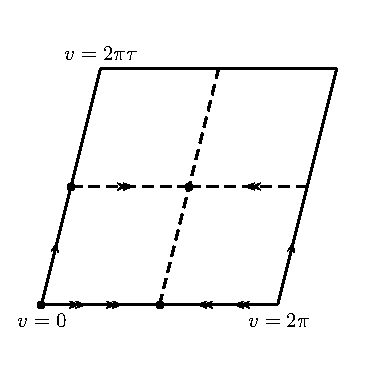
\includegraphics[width=.33\textwidth]{figures/torus_quotient}}
\caption{The pillow geometry is the quotient $T^2/\bZ_2$. The four points on the plane $0,z,1,\infty$ are mapped to the $\bZ_2$ fixed points $w=0,\pi,\pi(\tau+1),\pi\tau$ respectively. }\label{fig:pillow}
\end{figure}

As a power series expansion in $z$, ${\cal F}_c$ has radius of convergence 1, and is singular at $z=1$. The recurrence formula (\ref{zrecurr}) makes it clear that ${\cal F}_c$ can be analytically continued to the complex $z$-plane, except for a branch cut that extends from $1$ to $\infty$. This is not the full story, however, as ${\cal F}_c$ can be analytically continued beyond the branch cut on the $z$-plane. To fully exhibit the analytic property of the Virasoro conformal block, it is useful to map the Riemann sphere with the four marked points $0, z, 1, \infty$ to the ``pillow" geometry $T^2/\mathbb{Z}_2$, parameterized by the periodically valued complex coordinate $w\sim w+2\pi \sim w+2\pi \tau$ that is subject to the $\mathbb{Z}_2$ identification $w\sim -w$. It is also conventional to define the ``elliptic nome" $\mathfrak{q}=e^{\pi i \tau}$, where $\tau$ is related to $z$ by
\ie\label{tkkf}
\tau = i {K(1-z)\over K(z)},~~~ K(z) = {}_2F_1({1\over 2},{1\over 2};1;z).
\fe
The explicit map from the coordinate $u$ on the Riemann sphere to $w$ on the pillow is
\ie\label{pillowmapa}
w = {1\over (\theta_3(\tau))^2} \int_0^u {dx\over \sqrt{x(1-x)(z-x)}},
\fe
where $\theta_3(\tau) = \sum_{n=-\infty}^\infty \mathfrak{q}^{n^2}$ is one of the Jacobi theta functions. In the pillow frame, the four primary operators are inserted at the corners $w=0,\pi, \pi \tau, \pi(1+\tau)$, and the conformal block can be thought of as the propagator on the cylinder %\cite{Maldacena:2015iua}
\ie\label{piloo}
\langle\psi_{43}| \mathfrak{q}^{L_0 - {c\over 24}} |\psi_{12}\rangle = \sum_{n=0}^\infty a_n \mathfrak{q}^{h+n-{c\over 24}},
\fe
where $|\psi_{12}\rangle$ and $|\psi_{43}\rangle$ are the states created by a pair of primaries inserted at two corners of the pillow, projected onto the representation space of the Virasoro algebra with primary weight $h$, and the coefficients $a_n$ are functions of the weights $h_i, h$ and the central charge $c$. (\ref{piloo}) differs from the sphere 4-point block by a conformal anomaly factor (due to the Weyl transformation relating the flat metric on the $z$-plane to the flat metric on $T^2/\mathbb{Z}_2$),
\ie\label{pillowrep}
{\cal F}_c(h_1,h_2,h_3,h_4,h;z) = (\theta_3(\tau))^{{c\over 2} - 4(h_1+h_2+h_3+h_4)} z^{{c\over 24}-h_1-h_2} (1-z)^{{c\over 24} - h_3-h_4} \langle\psi_{43}| \mathfrak{q}^{L_0 - {c\over 24}} |\psi_{12}\rangle.
\fe

\begin{figure}[h!]
\centering
\subfloat{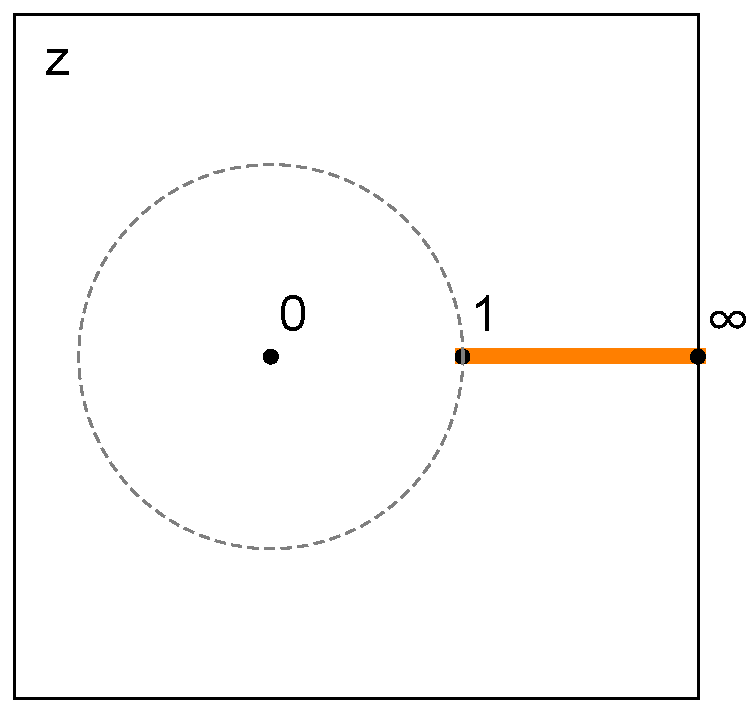
\includegraphics[width=.3\textwidth]{figures/zbranch.pdf}}~~~~~~~~~~~~~~~~~
\subfloat{
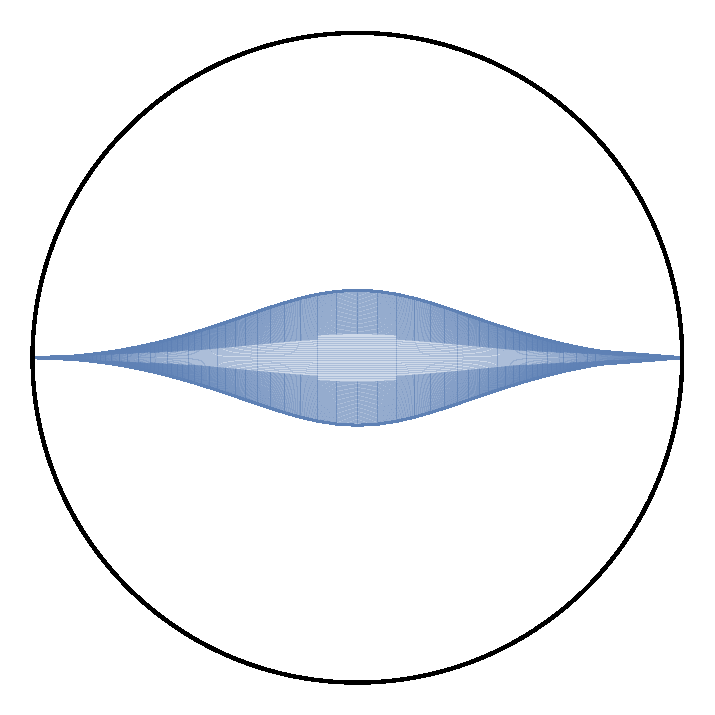
\includegraphics[width=.3\textwidth]{figures/qdisc.pdf}
}
\caption{The complex $z$-plane with a branch cut along $[1,\infty)$ is mapped to the eye-shaped region on the unit $q$ disc. The Virasoro conformal block can be analytically continued to the entire $q$ disc.}\label{fig:ellipticnome}
\end{figure}

The pillow representation of the conformal block (\ref{pillowrep}) exhibits several important properties. Firstly, as a series expansion in $\mathfrak{q}$, (\ref{piloo}) converges on the unit $\mathfrak{q}$-disc, and is holomorphic on the $\mathfrak{q}$-disc away from the origin. In other words, the domain of analyticity of ${\cal F}_c$ covers the entire complex $z$-plane and more: the complex $z$-plane only maps to an eye-shaped region on the $\mathfrak{q}$-disc. Note that $\mathfrak{q}$ can be expanded in $z$ as
\ie
\mathfrak{q} = {z\over 16} + {z^2\over 32} + {21 z^3\over 1024} + \cdots,
\fe
but the $\mathfrak{q}$-series converges much faster than the $z$-series at a generic point on the $z$-plane.

Secondly, the matrix element (\ref{piloo}) has the property that in the special case $h_1=h_4$, $h_2=h_3$, the coefficients $a_n$ are norms of Virasoro descendants of $|\psi_{12}\rangle$ and therefore non-negative (provided that the OPE involved is compatible with unitarity). 

Thirdly, (\ref{piloo}) simplifies in the $h\to \infty$ limit, with $c$ and $h_i$'s held fixed:
\ie\label{largehlim}
\lim_{h\to \infty} \langle\psi_{43}| \mathfrak{q}^{L_0 - {c\over 24}} |\psi_{12}\rangle = (16\mathfrak{q})^{h-{c\over 24}} \prod_{n=1}^\infty (1-\mathfrak{q}^{2n})^{-{1\over 2}}.
\fe
Heuristically, this can be understood based on the intuition that in the large $h$ limit, the external operators inserted at the corners of the pillow are unimportant; the square of the pillow block becomes the same as the pillow block of two copies of the CFT with $\mathbb{Z}_2$ twist fields inserted at each corner that exchanges the two CFTs (see section \ref{orbifoldsection}), which up to a conformal anomaly factor is equal to the torus character of the internal primary of weight $h$.

The large $h$ limit (\ref{largehlim}) together with the residues (\ref{hresiddu}) at the poles in $h$ allow us to derive a recurrence formula in $h$ rather than in $c$, of the form
\ie
{\cal F}_c(h_1,h_2,h_3,h_4,h;z) &= (\theta_3(\tau))^{{c-1\over 2} - 4(h_1+h_2+h_3+h_4)} z^{{c-1\over 24}-h_1-h_2} (1-z)^{{c-1\over 24} - h_3-h_2}  
\\
&~~~\times (16\mathfrak{q})^{h-{c-1\over 24}} \prod_{n=1}^\infty (1-\mathfrak{q}^{2n})^{-{1\over 2}} H_c(h_1,h_2,h_3,h_4,h;\mathfrak{q}),
\fe
where $H_c$ obeys
\ie\label{hcrecuf}
H_c(h_1,h_2,h_3,h_4,h;\mathfrak{q}) = 1 + \sum_{r,s\geq 1} {(16\mathfrak{q})^{rs}\over h-h_{r,s}} A_{rs}^cP_c^{rs} {h_1\brack h_2} P_c^{rs} {h_4\brack h_3} H_c(h_1,h_2,h_3,h_4,h_{r,s}+rs;\mathfrak{q}).
\fe
In practice we can use this relation to evaluate ${\cal F}_c$ efficiently, by first using (\ref{hcrecuf}) as a set of linear equations for $H_c(h_1,h_2,h_3,h_4,h_{r,s}+rs;\mathfrak{q})$ and solve for the latter over a finite set of $r,s$ subject to $rs\leq n$, up to order $\mathfrak{q}^n$, and then using (\ref{hcrecuf}) to generate $H_c$ for generic internal weight $h$ up to order $\mathfrak{q}^n$.



\newpage

\section{Riemann surfaces and modular invariance}
\label{riemsurfsec}

%In the string path integral based on the Polyakov action, a naive counting of degrees of freedom might suggest that one can use the diffeomorphism and Weyl gauge symmetry to fix the dynamical metric $g_{ab}$ to an arbitrary fiducial metric $\hat g_{ab}$. While this is indeed possible locally on the worldsheet, there may be global obstructions. Generally, it is only possible to gauge fix $g_{ab}$ to a family of fiducial metrics $\hat g_{ab}(t^k)$, where $t^k$ are a set of parameters that can be viewed as coordinates on a ``moduli space". 
%
%Further, after fixing $g_{ab} = \hat g_{ab}(t^k)$, there may be residual unfixed gauge redundancies, that generate the ``conformal Killing group". Infinitesimally, the conformal Killing group is generated by diffeomorphism parameters $\delta v^a$ and Weyl parameters $\delta\omega$, such that
%\ie\label{ckvdef}
%\delta \hat g_{ab} = -\hat\nabla_a v_b - \hat\nabla_b v_a + 2 \delta\omega \hat g_{ab}=0.
%\fe
%Evidently, $\delta\omega$ is then determined by $v^a$. A vector field $v^a$ that obeys (\ref{ckvdef}) is called a conformal Killing vector (field).






\subsection{The sphere}
\label{spheresec}

We begin with the genus $h=0$ case, in which case the Riemann surface is topologically a sphere. The Riemann sphere has no moduli, and every metric on the sphere can be put to the form of the Euclidean metric
\ie
ds^2 = dz d\bar z
\fe
by a Weyl transformation. More precisely, the $z$ coordinate chart $U$ covers the sphere minus one point. There is another coordinate chart $V$, parameterized by the complex coordinate $w$, such that on the overlap $U\cap V$, the two coordinates are related by $w=1/z$.% Clearly, $dz d\bar z$ and $dz' d\bar z' = |z|^{-4} dz d\bar z$ are related by a Weyl transformation.

The conformal Killing vector (CKV) is a linear combination of a (globally defined) holomorphic vector field and an anti-holomorphic vector field,
\ie
v^z(z) \partial_z + \widetilde v^{\bar z}(\bar z) \partial_{\bar z}.
\fe
On a different coordinate chart parameterized by $w$, the vector field is expressed as $v^w(w) \partial_w + \widetilde v^{\bar w}(\bar w) \partial_{\bar w}$, where $v^w(w)$ is related to $v^z(z)$ on the overlap of the coordinate charts by
\ie
v^w(w) = v^z(z){\partial w\over \partial z}.
\fe
On the Riemann sphere, a holomorphic vector field of the form $v^z(z) \partial_z$ on the chart $U$ would be written as
\ie
-w^2 v^z(1/w) \partial_w
\fe
on the chart $V$. $v^z(z)$ should be holomorphic on the entire complex $z$-plane, as is $-w^2 v^z(w)$ on the entire complex $w$-plane. This restricts $v^z(z)$ to be a quadratic polynomial,
\ie
v^z(z) = a_0 + a_1 z + a_2 z^2.
\fe
These CKVs generate a finite conformal Killing group transformation of the form
\ie\label{ckgelm}
z\mapsto z' = {\A z + \B \over \C z + \D},
\fe
where $\A,\B,\C,\D$ can be taken to be complex numbers with $\A\D-\B\C=1$. Further, flipping the signs of $\A,\B,\C,\D$ simultaneously does not change the transformation (\ref{ckgelm}), and preserves the condition $\A\D-\B\C=1$. Therefore, the conformal Killing group of the Riemann sphere is isomorphic to $PSL(2,\mathbb{C})$.


\subsection{The torus}
\label{torussec}

Next consider the genus $h=1$ case, where the Riemann surface is topologically a torus. Up to a Weyl transformation, the metric on the torus can always be put to the Euclidean form $ds^2=dz d\bar z$, but with the coordinate $z$ subject to the periodic identification
\ie\label{ziden}
z\sim z+2\pi \sim z+2\pi \tau,
\fe
where $\tau=\tau_1+i\tau_2$ for $\tau_1, \tau_2\in\mathbb{R}$, $\tau_2>0$. We could equivalently describe the torus via coordinate charts, but that would not be necessary. An alternative coordinate system $(\sigma^1, \sigma^2)$, where $\sigma^1$ and $\sigma^2$ are of periodicity $2\pi$, is related by
\ie
z = \sigma^1 + \tau \sigma^2,~~~ \bar z = \sigma^1 + \bar\tau \sigma^2,
\fe
so that the metric can be written as
\ie\label{dsigmam}
ds^2 = |d\sigma^1 + \tau d\sigma^2|^2.
\fe
$\tau$ is a complex parameter of the moduli space ${\cal M}_1$ of the torus as a Riemann surface. 

The only diffeomorphism that preserves the Euclidean metric up to a Weyl transformation with an identification of the form (\ref{ziden}) for {\it some} $\tau$ is a linear holomorphic map, of the form
\ie
z\mapsto z' = {z\over c\tau + d},
\fe
where $c$ and $d$ are a pair of coprime integers. Note that $z'$ is identified with $z'+2\pi$, and is also identified with $z'+2\pi \tau'$, for
\ie\label{psltz}
\tau' = {a\tau+b\over c\tau +d},
\fe
for another pair of integers $a, b$ such that $ad-bc=1$. Indeed, the torus with modulus $\tau$ and $\tau'$ are equivalent under a ``large" diffeomorphism and Weyl transformation. In terms of the $\sigma^a$ coordinates, it can be expressed as a map $(\sigma^1, \sigma^2) \mapsto (\sigma'^1, \sigma'^2)$, with
\ie
\begin{pmatrix} \sigma'^1 \\ \sigma'^2 \end{pmatrix} = \begin{pmatrix} a & -b \\ -c & d \end{pmatrix}  \begin{pmatrix} \sigma^1 \\ \sigma^2 \end{pmatrix} ,
\fe
which is a diffeomorphism for integers $a,b,c,d$ that obey $ad-bc=1$.
The metric (\ref{dsigmam}) can be written in $\sigma'^a$ coordinates as 
\ie
ds^2 = |c\tau+d|^2 |d\sigma'^1 + \tau' d\sigma'^2|^2.
\fe
Thus, we learn that the modulus $\tau$ should be identified up to $PSL(2,\mathbb{Z})$ transformations of the form (\ref{psltz}). The moduli space of the torus is then
\ie
{\cal M}_1 \simeq \{\tau \in \mathbb{C}\,| \,{\rm Im}\tau>0\}/PSL(2,\mathbb{Z}).
\fe
${\cal M}_1$ can be parameterized by $\tau$ in the fundamental domain (\ref{funddomaintor}), with the boundary $\partial {\cal F}$ identified using either $\tau\to \tau+1$ or $\tau \to -1/\tau$. The resulting space ${\cal M}_1$ may be viewed topologically as a sphere with a puncture at $\tau =i\infty$, corresponding to a singular limit of the torus modulus, and two special points $\tau=i$ and $\tau = e^{2\pi i/3}$ where the torus develops a $\mathbb{Z}_4$ and $\mathbb{Z}_6$ discrete rotation symmetry respectively.

The conformal Killing vector fields on the torus are easy to describe: they are simply constant vector fields. The conformal Killing group of the torus with generic $\tau$ is $T^2\rtimes \mathbb{Z}_2$, where the $T^2$ is the group of translations along the torus, and the $\mathbb{Z}_2$ is the orientation-preserving reflection symmetry $z\mapsto -z$.

\subsection{Genus $h\geq 2$}
\label{sec:ggttwors}

A general Riemann surface of arbitrary genus may be constructed by gluing together Riemann surfaces of lower genera using the ``plumbing fixture". Given two Riemann surfaces $\Sigma_1$ and $\Sigma_2$, of genus $h_1$ and $h_2$ respectively, we can choose a coordinate chart $U\subset \Sigma_1$ parameterized by $z$ on the unit disc, and another coordinate chart $V\subset \Sigma_2$ parameterized by $w$ on the unit disc, and identify a pair of annulus regions on the two discs using the map
\ie\label{wzqmap}
w = q/z,
\fe
for a nonzero complex parameter $q$ with $|q|\leq 1$. The identification produces a new Riemann surface $\Sigma$ of genus $h=h_1+h_2$. 

Similarly, one may start with a single Riemann surface $\Sigma$ of genus $h$, pick two coordinate charts $U$ and $V$, and cut out a hole on each and identify them along a pair of annulus regions using the map (\ref{wzqmap}), thereby producing a new Riemann surface $\Sigma'$ of genus $h'=h+1$.

We can give a rough count of the dimension $\mu_h$ of the moduli space ${\cal M}_h$ of the genus $h$ Riemann surface based on the plumbing construction. We can choose the center of the pair of discs $U$ and $V$ on $\Sigma_1$ and $\Sigma_2$, and the complex parameter $q$, giving a total of 3 complex parameters, or 6 real parameters. Thus, we expect $\mu_{h_1+h_2} = \mu_{h_1} + \mu_{h_2} + 6$, which leads to $\mu_h = 6h-6$. This answer is obviously incorrect for $h=0$ or 1, but is in fact the correct number of real moduli for $h\geq 2$.

A more explicit description of the genus $h$ Riemann surface, obtained by plumbing together Riemann spheres, is as follows. We begin with the Riemann sphere $\mathbb{C}\cup\{\infty\}$, and consider a set of $h$ loxodromic $PSL(2,\mathbb{C})$ elements $\C_1, \cdots, \C_h$. Each $\C_i$ acts on the complex coordinate $z$ by
\ie\label{clagz}
z\mapsto \C_i(z) = {a_i z + b_i \over c_i z + d_i},
\fe
with $a_i d_i - b_i c_i=1$, such that the $SL(2,\mathbb{C})$ matrix $\begin{pmatrix} a_i & b_i \\ c_i & d_i \end{pmatrix}$ has a pair of distinct eigenvalues $q_i, q_i^{-1}$ with $|q_i|<1$. Generically, there are no group relations among $\C_1, \cdots, \C_h$. Together they generate a free group $\Gamma$, known as the Schottky group, that acts on the Riemann sphere. The set $\Lambda$ of accumulation points of $\Gamma$ on the Riemann sphere is a certain Cantor set of measure zero. The quotient
\ie\label{sigmasch}
\Sigma = (\mathbb{C}\cup\{\infty\} - \Lambda)/\Gamma
\fe
is a Riemann surface of genus $h$. The Schottky group involves $3h$ complex parameters, but an overall conjugation by $PSL(2,\mathbb{C})$, the conformal Killing group of the Riemann sphere, produces an equivalent Schottky group action. Thus the moduli space of $\Sigma$ is parameterized by $3h-3$ independent complex parameters. In fact, each point of the genus $h$ Riemann surface moduli space ${\cal M}_h$ can be realized by a Schottky group through (\ref{sigmasch}). However, each Schottky group not only determines a Riemann surface, but also specifies a particular pair-of-pants decomposition of that Riemann surface. A given Riemann surface admits many different pair-of-pants decompositions, leading to discrete identifications of the Schottky parameters. One must also be careful with the boundary of the moduli space where the Riemann surface degenerates. As a result, the full geometry of the moduli space ${\cal M}_h$ is generally rather complicated for $h\geq 2$.

Another useful characterization of the moduli of a genus $h$ Riemann surface $\Sigma$ is through the period matrix. Pick a basis of 1-cycles $\A^I$, $\B_J$, such that their intersection numbers are
\ie
\A^I \cdot \A^J = \B_I \cdot \B_J = 0,~~~ \A^I\cdot \B_J = - \B_J\cdot \A^I = \delta_J^I.
\fe
There is a basis of holomorphic 1-forms $\omega_I$ on $\Sigma$ that obey
\ie\label{holoneformnorm}
\int_{\A^I} \omega_J = \delta^I_J.
\fe
The period matrix $\Omega$ is an $h\times h$ complex matrix whose entries are
\ie\label{periodmatdef}
\Omega_{IJ} = \int_{\B_I} \omega_J.
\fe
The cohomology class of $\omega_I$ can be written as $[\omega_I]=\check\A_I + \Omega_{IJ} \check\B^J$, where $(\check\A_I, \check\B^J)$ are the basis of integral cohomology classes dual to $(\A^I, \B_I)$. It follows from $\int_\Sigma \omega_I \wedge \omega_J=0$ that $\Omega_{IJ}$ is symmetric, and from the positive definiteness of $i\int_\Sigma \omega_I \wedge \overline{\omega_J}$ that ${\rm Im}(\Omega_{IJ})$ is a positive definite matrix.

$\Omega$ is defined up to the ambiguity of a symplectic change of basis of the 1-cycles $(\A^I, \B_J)$. Namely, with respect to the basis
\ie{}
\A'^I = D^I{}_J \A^J + C^{IJ} \B_J,~~~ \B'_I = B_{IJ} \A^J + A_I{}^J \B_J,
\fe
where $A,B,C,D$ are matrices with integer entries that obey
\ie\label{abcdmat}
DA^T - CB^T = \mathbb{I},~~~BA^T=AB^T, ~~~ DC^T=CD^T,
\fe
parameterizing an element of $Sp(2g,\mathbb{Z})$, the new period matrix is
\ie\label{spgzt}
\Omega' = (A\Omega+B) (C\Omega+D)^{-1}.
\fe
Note that $\Omega$ has a priori ${h(h+1)\over 2}$ independent complex entries, whose number coincides with the dimension of the moduli space ${\cal M}_h$ for $h\leq 3$, but exceeds ${\rm dim}({\cal M}_h)$ for $h\geq 4$. In the latter case, there are nontrivial constraints among $\Omega_{IJ}$.

An explicit formula that expresses the period matrix in terms of the Schottky parameters is as follows. The $PSL(2,\mathbb{C})$ transformation (\ref{clagz}) can be expressed as
\ie
z\mapsto \C_i(z),~~~ {\C_i(z) - \eta_i\over \C_i(z)-\xi_i} = q_i {z-\eta_i\over z - \xi_i}.
\fe
The components of the period matrix $\Omega_{IJ}$ in a corresponding symplectic basis are then given by
\ie
e^{2\pi i \Omega_{IJ}} = q_I^{\delta_{IJ}}\prod_{\C\in \Gamma_{IJ}} {(\C(\eta_I) - \eta_J) (\C(\xi_I) - \xi_J)\over (\C(\eta_I) - \xi_J) (\C(\xi_I) - \eta_J)},
\fe
where $\Gamma_{IJ}$ is defined to be the subset of the Schottky group $\Gamma=\langle \C_1,\cdots,\C_h\rangle$ that consists of group elements that do not end with $\C_I^{\pm 1}$ on the right of its word, nor $\C_J^{\pm 1}$ on the left of its word. In the case $I=J$, the identity group element is also excluded from $\Gamma_{IJ}$ (but is included when $I\not=J$).



\subsection{Modular invariance of 2D CFT}
\label{modularsec}

There is a natural way to extend the definition of correlation functions of local operators in a 2D CFT to any compact oriented surface $\Sigma$ equipped with a Riemannian metric, at least in the case $c=\widetilde c$ where gravitational anomalies are absent, as follows. 

Firstly, note that up to the Weyl anomaly factor (\ref{weylangen}) which depends only on the central charge $c$ and not any further details of the CFT, the partition function on $\Sigma$ depends only on the equivalence class of metrics with respect to Weyl transformation, i.e. the structure of $\Sigma$ as a Riemann surface. Likewise, under a Weyl transformation of the metric, a correlation function of local operators ${\cal O}_1,\cdots, {\cal O}_n$ on $\Sigma$ acquires the same Weyl anomaly factor, provided that the Weyl transformation is trivial in a small neighborhood of the local operators. For our purpose, it suffices to assume that each operator ${\cal O}_a$ is inserted at the origin of a disc $D_a\subset \Sigma$ on which the metric is flat, so that there is no ambiguity with regard to the state created by ${\cal O}_a$ in radial quantization on $D_a$.

If $\Sigma$ is a surface of genus $h>1$, we can decompose it into $2h-2$ ``pairs of pants", joined along their boundary circles $C_k$, $k=1,\cdots, 3h-3$. If $\Sigma$ has genus $h=1$ then it suffices to represent $\Sigma$ as a cylinder with two boundary circles identified. The metric in a neighborhood of each circle $C_k$, up to a Weyl transformation, can be put in the form of a standard Euclidean cylinder parameterized by $(\tau, \sigma)$, $\sigma\sim \sigma+2\pi$, $\tau \in (-\epsilon, \epsilon)$ for some $\epsilon>0$, such that $C_k$ corresponds to the equal time slice $\tau=0$. We can then insert a complete basis of states along $C_k$, and express the correlation function $\langle {\cal O}_1\cdots {\cal O}_n\rangle_\Sigma$ in terms of correlation functions of local operators on pairs of pants or cylinders, with appropriate CFT states assigned to the boundary circles. The correlation functions on pairs of pants or cylinders are conformally equivalent to correlators on the sphere or the plane, which are then determined by the structure constants as described in section \ref{confblocksec}.

Equivalently, we may view the surface $\Sigma$ with $n$ local operator insertions as a surface with $n$ ``punctures". We can decompose the punctured surface into $2h-2+n$ pairs of pants, with $n$ of the boundary circles shrunk to points. The $n$-point function on $\Sigma$ is then decomposed into the product of $2h-2+n$ three-point functions, suitably Weyl transformed, summed over the basis of states inserted along $3h-3+n$ circles.

The consistency in defining correlation functions on $\Sigma$ requires that different pair-of-pants decompositions of the $n$-punctured surface $\Sigma$ result in the same answer for the correlation function. If $\Sigma$ is topologically a sphere, this consistency condition is equivalent to the crossing equation for the conformal block decomposition of sphere 4-point functions, or the associativity of the OPE. 


\begin{figure}[h!]
\centering
\subfloat{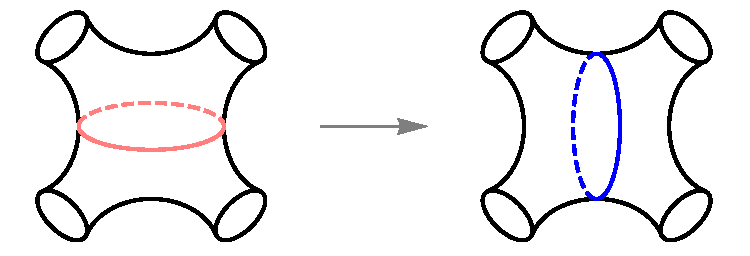
\includegraphics[width=.7\textwidth]{figures/spherecross.pdf}}
\caption{The crossing move relating two different pair-of-pants decompositions of the four-holed sphere.}\label{fig:spherecross}
\end{figure}


\begin{figure}[h!]
\centering
\subfloat{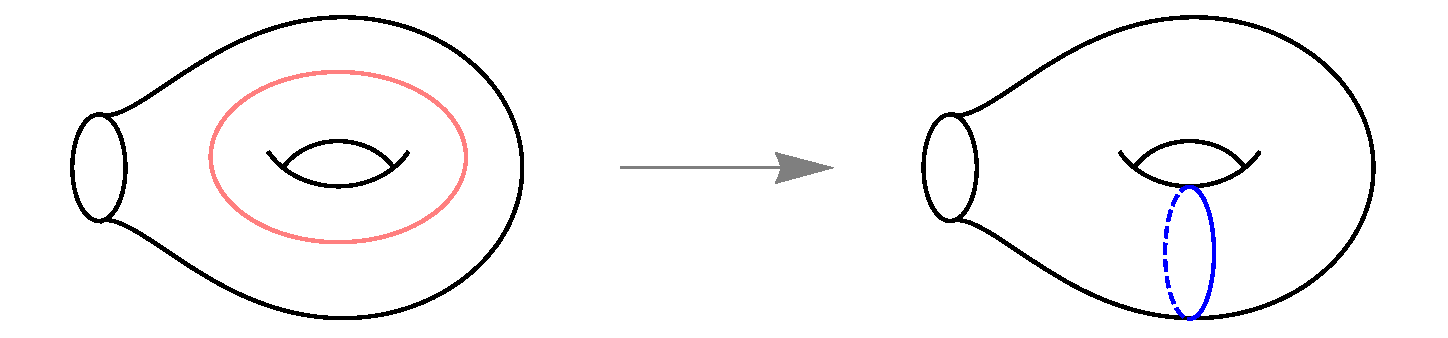
\includegraphics[width=.7\textwidth]{figures/toruscross.pdf}}
\caption{The crossing move relating two different pair-of-pants decompositions of the one-holed torus.}\label{fig:toruscross}
\end{figure}

If $\Sigma$ is a torus with one puncture, i.e. $h=n=1$, we can cut the torus along either the $\A$ circle or the $\B$ circle as shown in Figure \ref{fig:toruscross}, and decompose the torus one-point function into a sum of sphere three-point functions. More explicitly, as will be discussed in detail in section \ref{torussec}, the torus may be parameterized by the complex coordinate $z$, subject to periodicity $z\sim z+2\pi \sim z+2\pi\tau$, for a complex modulus parameter $\tau=\tau_1+i\tau_2$ with $\tau_2>0$. We can write the 1-point function of an operator ${\cal O}(z,\bar z)$ on the torus of modulus $\tau$, equipped with the Euclidean metric $ds^2 = dz d\bar z$, as\footnote{The relation between the torus 1-point function and the trace on the RHS of (\ref{onepointtrace}) will be modified in ghost CFTs. For instance, in the $bc$ system to be discussed in section \ref{brstwssec}, one must insert $(-)^{N_{bc}}$ into the trace, where $N_{bc}$ is the $bc$ ghost number.}
\ie\label{onepointtrace}
\left\langle {\cal O}(z,\bar z)\right\rangle_{T^2(\tau)} = {\rm Tr}_{\cal H} {\cal O}(z,\bar z) \, e^{-2\pi \tau_2 H + 2\pi i \tau_1 P} = {\rm Tr}_{\cal H} {\cal O}(z,\bar z) \, e^{2\pi i \tau (L_0 - {c\over 24}) -2\pi i \bar\tau (\widetilde L_0 - {\widetilde c\over 24})},
\fe
where ${\cal H}$ is the Hilbert space of the CFT on the unit circle, $H$ and $P$ are the energy and momenta on the circle, related to Virasoro generators $L_0$ and $\widetilde L_0$ via (\ref{hpid}). ${\cal O}(z,\bar z)$ on the RHS is viewed as an operator inserted at the point $z$ on the cylinder.

It follows from translation symmetry along the torus that $\left\langle {\cal O}(z,\bar z)\right\rangle_{T^2(\tau)}\equiv f_{\cal O}(\tau, \bar\tau)$ is independent of $z, \bar z$. Assuming that ${\cal H}$ only consists of integer spin states, we have 
\ie\label{torusshift}
f_{\cal O}(\tau+1, \bar\tau+1) = f_{\cal O}(\tau, \bar\tau).
\fe
The equivalence of cutting along $\A$ versus $\B$ circle, on the other hand, implies
\ie\label{tousmod}
f_{\cal O}(-1/\tau, -1/\bar\tau) = e^{{\pi i\over 2}(h-\widetilde h)} (-i\tau)^h (i\bar\tau)^{\widetilde h} f_{\cal O}(\tau, \bar\tau),
\fe
where $(h, \widetilde h)$ are the conformal weights of ${\cal O}$. On the RHS, $-i\tau$ has positive real part, and its power is defined with a branch cut chosen to lie on the left half complex plane. (\ref{tousmod}) can also be understood from the fact that the torus of modulus $\tau$ is conformally equivalent to the torus with modulus $\tau'=-1/\tau$, via the map $z\mapsto z'=z/\tau$. We will refer to the conditions (\ref{torusshift}) and (\ref{tousmod}) as the modular invariance of the torus one-point function.

%\begin{figure}[h!]
%\centering
%\subfloat{\includegraphics[width=\textwidth]{figures/genustwocross.pdf}}
%\caption{A sequence of simple crossing moves that relate two different pair-of-pants decompositions of a genus two surface.}\label{fig:genustwocross}
%\end{figure}

It can be shown that any two different pair-of-pants decompositions of the $n$-punctured surface $\Sigma$ can be related by a sequence of simple crossing moves: either the crossing move on the 4-punctured sphere (Figure \ref{fig:spherecross}), or that of the 1-punctured torus (Figure \ref{fig:toruscross}).\footnote{Hatcher and Thurston, Topology 19, 221 (1980) \cite{Hatcher_1980}.} %A genus two example is shown in Figure \ref{fig:genustwocross}. 
Consequently, the consistency of the $n$-point function on $\Sigma$ follows from the crossing invariance of all sphere 4-point functions together with the modular invariance of all torus 1-point functions.

Modular invariance puts highly nontrivial constraints on a CFT. For instance, while free boson CFT is a modular invariant theory, its $k=0$ sector, generated by operators of the form $\partial^n \bar\partial^m X$ and their normal order products, closes under OPE but is not modular invariant. 

The integer spin (NS,NS) sector states of the free fermion CFT close under OPE, but is not modular invariant by itself. A modular invariant CFT with $c=\widetilde c={1\over 2}$, known as the critical Ising model, can be constructed by combining the integer spin (NS,NS) sector and (R,R) sector states (Appendix \ref{isingcft}). Such a construction is known as the {\it diagonal} Gliozzi-Scherk-Olive (GSO) projection. The worldsheet CFT of type II superstrings, on the other hand, is a non-unitary theory defined with the {\it chiral} GSO projection (section \ref{sec:chiralgsosup}) on the free fermions as well as superconformal ghosts, in which a subset of integer spin states in the (NS,NS), (NS,R), (R,NS), (R,R) sectors are included in the spectrum.








\newpage

\section{2D free field theories}

\subsection{Free bosons}
\label{sec:freeboson}

As a first example, let us consider the theory of a free massless scalar field in 2D, described by the action
\ie\label{xxactfbs}
S = {1\over 4\pi \A'} \int d^2\sigma \partial_a X \partial^a X = {1\over 2\pi \A'} \int d^2z \partial X \bar\partial X.
\fe
Here we adopt a normalization convention of the field $X$ so as to agree with one of the scalar fields in the Polyakov action in conformal gauge. Recall that the measure $d^2z$ is defined with the convention (\ref{dsqzconv}).

We will write $w=\sigma + i\tau$ for the complex coordinate on the Euclidean cylinder, related to the coordinate $z$ of the complex plane by the exponential map $z=e^{-iw}$. We will denote by $t$ the time coordinate on the Lorentzian cylinder, which is related to the Euclidean time $\tau$ by $t= - i\tau$.

The Hamiltonian on the cylinder is
\ie
H = \int_0^{2\pi} d\sigma \left[ \pi \A' \Pi^2 + {1\over 4\pi \A'} (\partial_\sigma X)^2 \right],
\fe
where $\Pi = {1\over 2\pi \A'}\partial_t X$ is the canonical momentum density. At time $t=0$, we can decompose $X(\sigma,t=0)$ and $\Pi(\sigma,t=0)$ into their Fourier modes,
\ie\label{xpifour}
& X(\sigma,t=0) = \hat x + i \sqrt{\A'\over 2} \sum_{n\not=0} {\A_n - \widetilde \A_{-n} \over n} e^{in\sigma} ,
\\
& \Pi(\sigma,t=0) = {\hat k\over 2\pi} + {1\over 2\pi \sqrt{2\A'}} \sum_{n\not=0} (\A_n + \widetilde \A_{-n}) e^{in\sigma},
\fe
where the coefficients $\hat x$, $\hat k$, $\A_n$, $\widetilde \A_n$ turn into operators acting on the Hilbert space of the free boson theory on the unit circle. It follows from the equal time canonical commutation relation
\ie{}
[X(\sigma,t), \Pi(\sigma',t)] = i \delta(\sigma-\sigma'),~~~[X(\sigma,t), X(\sigma',t)] = [\Pi(\sigma,t), \Pi(\sigma',t)] = 0
\fe
that the non-vanishing commutators among $\hat x$, $\hat k$, $\A_n$, $\widetilde \A_n$ are
\ie\label{bosmodexk}
[\hat x,\hat k]= i,~~~ [\A_n, \A_m] = [\widetilde\A_n, \widetilde \A_m] = n \delta_{n,-m}.
\fe
The oscillator $\A_n$ (or $\widetilde \A_n$) with negative $n$ may be viewed as $\sqrt{|n|}$ times the creation operator that creates a massless left (or right) moving particle on the circle that carries $|n|$ units of momentum. The oscillator $\A_n$ (or $\widetilde \A_n$) with positive $n$ is $\sqrt{n}$ times the annihilation operator of the corresponding mode. The Hilbert space of the free boson CFT on the circle was already constructed in (\ref{focks}). In the oscillator notation, we can write a basis of states as
\ie\label{fockbas}
|k;\{n_i, \widetilde n_i\}_{i\geq 1} \rangle = \A_{-n_1}\A_{-n_2}\cdots \widetilde \A_{-\widetilde n_1} \widetilde \A_{-\widetilde n_2}\cdots |k\rangle,
\fe
where $n_i$ and $\widetilde n_i$ are a set of positive integers. The oscillator vacuum $|k\rangle$ has eigenvalue $k$ with respect to $\hat k=\int_0^{2\pi} \Pi d\sigma$, and is annihilated by all of $\A_n, \widetilde \A_n$ with positive $n$.

What operators are (\ref{fockbas}) mapped to under the state/operator correspondence? A naive guess is
\ie\label{prodnaive}
\partial^{n_1} X \partial^{n_2} X \cdots \bar \partial^{\widetilde n_1} X \bar\partial^{\widetilde n_2} X \cdots e^{ikX},
\fe
which has the correct transformation property under the global symmetry that shifts $X$, and the expected $n_i$, $\widetilde n_i$ dependence in its conformal weight. However, as a product of field operators at coincident points, (\ref{prodnaive}) is not well defined as a local operator, unless a suitable normal ordering or regularization prescription is adopted.

Indeed, any correlation function that involves a pair of free boson field operators $X(z_1,\bar z_1)$ and $X(z_2, \bar z_2)$ has a divergence in the $z_1\to z_2$ limit, of the form
\ie
\left\langle X(z_1,\bar z_1) X(z_2, \bar z_2)\cdots\right\rangle = -{\A'} \log |z_{12}| \langle \cdots \rangle + ({\rm regular~terms~in~}z_1\to z_2 ~{\rm limit}),
\fe
due to the Wick contraction of $X(z_1,\bar z_1)$ with $X(z_2, \bar z_2)$. If we subtract off the Green function $-\A' \log |z_{12}|$ from $X(z_1,\bar z_1) X(z_2, \bar z_2)$ to define the normal ordered product
\ie
:X(z_1,\bar z_1) X(z_2, \bar z_2): \equiv X(z_1,\bar z_1) X(z_2, \bar z_2) + \A' \log |z_1-z_2|,
\fe
then 
\ie
:X^2(z_2, \bar z_2): \equiv \lim_{z_1\to z_2} :X(z_1,\bar z_1) X(z_2, \bar z_2):
\fe
is a well defined local operator. We can also phrase this in terms of the OPE
\ie\label{xxop}
X(z,\bar z) X(0) &= -\A' \log|z| + :X(z,\bar z) X(0): 
\\
& = -\A' \log|z| + \sum_{n,m\geq 0} {z^n \bar z^m \over n! m!} :X\partial^n \bar\partial^m X(0):.
\fe
The second line is organized as an expansion in powers of $z, \bar z$, with operators of increasing conformal weights.

The normal ordering can be generalized to
\ie
:{\cal F}[X]: \,\equiv \exp\left\{ {1\over 2} \int d^2z_1 d^2 z_2 \,\A'\log|z_{12}| {\delta\over \delta X(z_1,\bar z_1)} {\delta\over \delta X(z_2,\bar z_2)}\right\} {\cal F}[X],
\fe
where the functional ${\cal F}[X]$ may be taken to be product of the free boson field $X$ and its derivatives, and the functional derivative $\delta/\delta X$ is normalized such that
\ie
{\delta \over \delta X(z,\bar z) } X(z',\bar z') = \delta^2(z-z').
\fe
From now on, when we write the normal ordered product of free fields and their derivatives at the same position, the normal ordering sign will be omitted. 

Now consider the OPE of $X(z,\bar z)$ with a general operator ${\cal O}(0)$ at the origin. The free boson equation of motion, $\partial\bar\partial X(z,\bar z)=0$, holds away from $z=0$. In particular, $\partial X(z)$ is meromorphic with a Laurent expansion in $z$, and likewise $\bar\partial X(\bar z)$ is anti-meromorphic. Thus we can write
\ie\label{xoope}
X(z,\bar z) {\cal O}(0) = \left[ \hat x - {i\A'\over 2} \hat k \log|z|^2+ i \sqrt{\A'\over 2} \sum_{n\not=0} {1\over n} \left( {\A_n\over z^n} + {\widetilde \A_n\over \bar z^n} \right) \right] {\cal O}(0),
\fe
where $\hat x, \hat k, \A_n, \widetilde \A_n$ are regarded as operators acting on ${\cal O}(0)$. Under the state/operator map, $z=e^{-iw}$, (\ref{xoope}) is equivalent to the action of the operator $X$ inserted at $w$ on the Euclidean cylinder, acting on the state $|{\cal O}\rangle$, and $\hat x, \hat k, \A_n, \widetilde \A_n$ coincide with those defined by the canonical quantization of (\ref{xpifour}). 

When it is understood that an operator is inserted at the origin, one often writes (\ref{xoope}) by omitting ${\cal O}(0)$ on both sides of the equation. We can also express $\hat k$, $\A_n$, $\widetilde \A_n$ as
\ie\label{kalpx}
& \hat k = \oint {dz\over 2\pi i} {2i\over \A'}\partial X = -\oint {d\bar z\over 2\pi i} {2i\over \A'}\bar\partial X,
\\
& \A_n = i \sqrt{2\over \A'} \oint {dz\over 2\pi i } z^n \partial X,~~~ \widetilde \A_n = -i \sqrt{2\over \A'} \oint {d\bar z\over 2\pi i } \bar z^n \bar\partial X,~~~n\not=0,
\fe
where the contour is always taken to be counterclockwise around the origin unless otherwise noted.
Sometimes one also defines $\A_0 = \widetilde \A_0 = \sqrt{\A'\over 2} \hat k$, so that the second line of (\ref{kalpx}) holds for all integer $n$. 

The state/operator correspondence maps the identity operator 1 to the ground state $|0;0\rangle$, as both are annihilated by $\A_n, \widetilde \A_n$ for $n\geq 1$, as well as by $\widehat k$. From the first line of (\ref{kalpx}) and using the OPE of $\partial X(z)$ with $e^{ikX(0)}$, we have
\ie
\hat k e^{ikX(0)} 
\,= \oint {dz\over 2\pi i}\left[ {k\over z} e^{ik X(0)} + {2i\over \A'} :\partial X(z) e^{ikX(0)}: \right]
= k e^{ikX(0)},
\fe
we see that the operator $e^{ikX(0)}$ should be identified with the oscillator ground state $|k\rangle$. By repeatedly acting on $\partial^{n_1} X\cdots \bar\partial^{\widetilde n_1} X\cdots e^{ikX(0)}$ with $\A_n$ or $\widetilde\A_n$ with negative $n$, we see that the Fock state (\ref{fockbas}) corresponds to the operator
\ie
\left[\prod_j {i \sqrt{2/\A'}\over (n_j-1)!} \partial^{n_j} X \right]\left[ \prod_{\widetilde j} {i \sqrt{2/\A'}\over (\widetilde n_{\widetilde j}-1)!} \bar\partial^{\widetilde n_{\widetilde j}} X \right] e^{ikX(0)}.
\fe
The stress-energy tensor $T(z)$ and $\widetilde T(\bar z)$ of the free boson theory are given by
\ie\label{clstr}
& T= -{1\over \A'}\partial X\partial X,~~~ \widetilde T= -{1\over \A'}\bar\partial X\bar \partial X.
\fe
By explicitly computing the OPE with $T(z)$ and $\widetilde T(\bar z)$, one can see that $e^{ikX(0)}$, for instance, is a primary of weight $h=\widetilde h = {\A' k^2\over 4}$. Moreover, the stress-energy tensor (\ref{clstr}) obeys the OPE algebra (\ref{ttopes}) with central charge $c=1$.



\subsection{Free boson on a Riemann surface}

The torus correlator of the free boson CFT can be calculated using Wick contractions,
\ie\label{tachtoruscorr}
& \left\langle \prod_{i=1}^n e^{ik_i X(z_i,\bar z_i)}  \right\rangle_{T^2}
\\
& = 2\pi \delta(\sum k_i) Z_X'(\tau,\bar\tau) \exp\left[ - \A' \sum_{1\leq i<j\leq n} k_i k_j G(z_{ij},\bar z_{ij}) - {\A'\over 2} \sum_{i=1}^n k_i^2 G^r(0) \right],
\fe
where $Z_{X}'$ is the torus partition function of $X^\mu$ divided by the target space volume,
\ie
Z_{X}'(\tau,\bar\tau) = \int {d k\over 2\pi} e^{- \pi \A' k^2 \tau_2} |\eta(\tau)|^{-2}.
\fe
$G(z,\bar z)$ is the two-point function of the nonzero modes of the free boson on the torus, which obeys
\ie\label{greenbsocnd}
& \partial_z \bar\partial_{\bar z} G(z,\bar z) = -\pi \delta^2(z) + {1\over 8\pi \tau_2},
\\
& \int_{T^2} d^2z\, G(z,\bar z) = 0.
\fe
The solution is given by
\ie
G(z,\bar z) = - \log\left| \theta_1(z|\tau) \right| + {({\rm Im}(z))^2 \over 4\pi\tau_2} + k(\tau,\bar\tau),
\fe
where $k(\tau,\bar\tau)$ is independent of $z$ and serves to ensure the second condition in (\ref{greenbsocnd}). $\theta_1$ is one of the Jacobi theta functions, that admits the sum and product representations
\ie
\theta_1(z|\tau) &= i \sum_{n\in\mathbb{Z}} (-)^n e^{\pi i \tau (n-{1\over 2})^2 + i z (n-{1\over 2})}
\\
&= 2 q^{1\over 8} \sin({z\over 2}) \prod_{m=1}^\infty (1-q^m)(1-e^{iz} q^m) (1-e^{-iz} q^m),
\fe 
where we wrote $q=e^{2\pi i\tau}$ in the second line.
Note that $\theta_1$ as a function of $z$ is not well defined on the torus: it obeys $\theta_1(z+2\pi |\tau) = - \theta_1(z|\tau)$ and $\theta_1(z+2\pi\tau|\tau) = - e^{-i(z+\pi\tau)}\theta_1(z|\tau)$.

Finally, the appearance of $G^r(0)$ in (\ref{tachtoruscorr}), given by
\ie\label{gregss}
G^r(0) = \lim_{z\to 0} \Big[ G(z,\bar z) + \log|z|\Big],
\fe
is due to our regularization scheme in the definition of the vertex operator $e^{ik\cdot X}$. Due to the spacetime momentum conservation, we can equivalently remove $G^r$ and replace $G$ in (\ref{tachtoruscorr}) by
\ie\label{gprimetorus}
G'(z,\bar z) &= G(z,\bar z) - G^r(0) 
\\
&= - \log\left| {\theta_1(z|\tau)\over \partial_z \theta_1(0|\tau)} \right| + {({\rm Im}(z))^2 \over 4\pi\tau_2}.
\fe

%\subsubsection{Free boson on a higher genus surface}

More generally, on a genus $h$ surface $\Sigma$ equipped with a Hermitian metric $ds^2 = 2 g_{z\bar z} dzd\bar z$, the free boson correlator is computed as
\ie\label{highergbosonco}
&\left\langle  \prod_{i=1}^n e^{ik_i\cdot X(z_i,\bar z_i)} \right\rangle_\Sigma
\\
&= 2\pi \delta(\sum k_i) 
Z_X'(\Sigma)
\exp\left[ - \A' \sum_{1\leq i<j\leq n}k_i k_j G(z_i, \bar z_i; z_j, \bar z_j) - {\A'\over 2} \sum_{i=1}^n k_i^2 G^r(z_i,\bar z_i) \right],
\fe
where $Z_X'$ is the partition function $Z_X(\Sigma)$ of (\ref{fzxform}) divided by the target space volume. $G$ is the two-point function of the {\it nonzero modes} of $X$, which obeys
\ie\label{greeneqn}
& \partial_z \bar\partial_{\bar z} G(z, \bar z; w, \bar w) = -\pi \delta^2(z-w) + {\pi g_{z\bar z}(z,\bar z) \over A_\Sigma},
\\
& \partial_z \bar\partial_{\bar w} G(z, \bar z; w, \bar w) = \pi \delta^2(z-w) - \pi \sum_{I,J} \omega_I(z) (({\rm Im} \Omega)^{-1})^{IJ} \overline{\omega_J}(\bar w),
\\
& \int_\Sigma d^2z \sqrt{|g(z,\bar z)|} \, G(z,\bar z;w,\bar w) = 0.
\fe
Here $\sqrt{|g|} = g_{z\bar z}$, $A_\Sigma = \int_\Sigma d^2z \sqrt{|g|}$ is the area of $\Sigma$, and $\omega_I$ ($I=1,\cdots,h$) are a basis of holomorphic 1-forms used to define the period matrix $\Omega_{IJ}$ as in (\ref{holoneformnorm}), (\ref{periodmatdef}). The solution can be put to the form
\ie\label{greenhigherg}
G(z, \bar z; w, \bar w) = - \log |E(z,w)| - \pi \sum_{I,j} {\rm Im}\int_w^z \omega_I\, (({\rm Im} \Omega)^{-1})^{IJ}\, {\rm Im}\int_w^z \omega_J + \rho(z,\bar z) + \rho(w,\bar w),
\fe
where $E(z,w)$ is the prime form defined in (\ref{ezwprime}), and $\rho$ depends on the choice of the Hermitian metric $g$.

$G^r$ in (\ref{highergbosonco}) is defined similarly to (\ref{gregss}),
\ie
G^r(z,\bar z) = \lim_{w\to z} \left[ G(z,\bar z;w,\bar w) +\log |z-w| \right].
\fe
It once again follows from momentum conservation that the function $\rho$ appearing in (\ref{greenhigherg}) drops out of (\ref{omegadetex}).






\subsection{Free fermions}
\label{freeferm}

The 1+1 dimensional free massless fermion theory in a general background metric $g_{ab}$ can be described by the covariant action
\ie\label{twodfermact}
S = -{i\over 4\pi} \int d^2\sigma \sqrt{-g} \, \psi\Gamma^a \nabla_a^{\rm spin} \psi.
\fe
$\psi$ is a Grassmann-odd 2-component spinor field, whose components are denoted $\psi_\A$, $\A=\pm$. The spinor index can be raised or lowered according to the convention $\psi^\A = \epsilon^{\A\B}\psi_\B$, $\epsilon^{+-} = \epsilon_{+-}=1$. Unless otherwise noted, the contraction of spinor indices is from upper left to lower right, e.g. $(\psi \chi) \equiv \psi^\A \chi_\A$, $(\psi\Gamma^a\chi) \equiv \psi^\A (\Gamma^a)_\A{}^\B \chi_\B$, etc. The matrices $\Gamma^a$ are dependent on $\sigma$ and obey $\{\Gamma^a, \Gamma^b\} = 2 g^{ab}$.
They are related to the standard 2D gamma matrices $\hat \Gamma^i$ by (\ref{gammacurved}), 
where $e_i{}^a$ is the inverse frame field, related to the metric by (\ref{framevardef}).
Our convention for $\hat \Gamma^i$ is such that in light cone coordinates $\sigma^\pm = \sigma \pm t$, the non-vanishing components of $\hat\Gamma^\pm$ are 
\ie
(\hat\Gamma^+)_{++} = (\hat\Gamma^-)_{--} = 2i .   %used to be -2
\fe
The spin connection $\nabla_a^{\rm spin}$ is defined as in (\ref{spinconndef}).
 

Note that in 2D, since $\psi\hat \Gamma_{i}\psi\equiv 0$, the spin connection term involving $\omega_a{}^{ij}$ does not contribute to the action (\ref{twodfermact}), and so we can in fact replace $\nabla_a^{\rm spin}$ by $\partial_a$ in (\ref{twodfermact}). However, $\omega_a{}^{ij}$ does enter the equation of motion, which is given by
\ie\label{fermeom}
\Gamma^a \nabla_a^{\rm spin} \psi = 0.
\fe
The classical stress-energy tensor is
\ie
T_{ab} = {2\pi \over \sqrt{-g}} e^i{}_{(a} {\delta S\over \delta e^i{}^{b)}} = - {i\over 2}\left( \psi \Gamma_{(a} \partial_{b)}\psi - g_{ab} \psi\Gamma^c\partial_c \psi \right),
\fe
which is conserved and traceless up to the equation of motion (\ref{fermeom}).

Now specializing to the 2D Minkowskian worldsheet, the free fermion action can be written as
\ie\label{psipmconvac}
S = - {1\over 2\pi} \int d^2\sigma \left( \psi_+ \partial_- \psi_+ + \psi_- \partial_+ \psi_-\right),
\fe
with the stress-energy tensor
\ie
T_{++} = -{1\over 2} \psi_+ \partial_+ \psi_+,~~~ T_{--} = -{1\over 2} \psi_- \partial_- \psi_-.
\fe
Let us consider the canonical quantization of this system on the cylinder, parameterized by $(\sigma, t)$ with $\sigma\sim \sigma+2\pi$. The canonical momentum density conjugate to $\psi_\pm$ is
\ie
\Pi^\pm_\psi = S{\overleftarrow\delta \over \delta \partial_t\psi_\pm} = \pm {1\over 4\pi} \psi_\pm.
\fe
According to the terminology of Dirac, these canonical momenta obey ``second-class primary constraints"
\ie\label{chicons}
\chi_\pm \equiv \Pi_\psi^\pm \mp {1\over 4\pi} \psi_\pm = 0,
\fe
with the equal-time Poisson anti-bracket
\ie
K_\pm(\sigma,\sigma')\equiv \{ \chi_\pm(\sigma), \chi_\pm(\sigma') \}^{\rm P} = \mp {1\over 2\pi} \delta(\sigma-\sigma').
\fe
Here the Poisson anti-bracket is computed by pretending that $\psi_\pm$ and $\Pi_\pm$ are independent variables. The classical Dirac bracket between a pair of functionals $\xi$ and $\eta$ of $\psi_\pm(\sigma)$ and $\Pi_\pm(\sigma)$ at time $t=0$, that consistently takes into account the constraint (\ref{chicons}), is then defined by
\ie
\{ \xi, \eta \}^{\rm D} &= \{\xi, \eta\}^{\rm P} - \int d\sigma \{\xi, \chi_\pm(\sigma) \}^{\rm P} K_\pm^{-1} \{\chi_\pm(\sigma), \eta\}^{\rm P},
\fe
where $K_\pm^{-1} = \mp 2\pi$ is the inverse of the operator $K_\pm$ defined by convolution with the integration kernel $K_\pm(\sigma,\sigma')$. This leads to
\ie
\{ \psi_\pm (\sigma), \psi_\pm(\sigma') \}^{\rm D} = \pm 2\pi \delta(\sigma-\sigma').
\fe
The canonical quantization proceeds by promoting $\psi_\pm(\sigma)$ to operators that obey the anti-commutators
\ie\label{psipsicom}
\{ \psi_\pm (\sigma), \psi_\pm(\sigma') \} = \pm 2\pi i \delta(\sigma-\sigma').
\fe
A priori there is an ambiguity in the choice of periodic boundary condition for the field $\psi_\pm(\sigma)$, namely we only need to demand that $T_{++}$ and $T_{--}$ are periodic under the shift $\sigma\to \sigma + 2\pi$, whereas $\psi_+$ and $\psi_-$ may independently be either periodic or anti-periodic. If the fermion field is periodic in a given state, we refer to that state as belonging to the ``Ramond sector", or R sector. If the fermion field is anti-periodic, we refer to the state as in the ``Neveu-Schwarz sector", or NS sector. A priori, the Hilbert space of the free fermion theory on the cylinder may involve states in either (NS,NS), (NS,R), (R,NS), or (R,R) sectors, where the notation is such that (NS,R) for instance  refers to a sector in which $\psi_+$ is anti-periodic and $\psi_-$ is periodic. In order for the CFT to have closed OPE algebra and the property of modular invariance, the actual Hilbert space of the CFT on the circle, which is in correspondence with local operators, should only include a subset of all possible states in the various sectors. Those states excluded from this Hilbert space may be interpreted as defect operators (Appendix \ref{tdlsec}).

Let us consider the Fourier expansion of $\psi_-(\sigma)$ at $t=0$,
\ie\label{psicylex}
\psi_-(\sigma) = e^{-{\pi i\over 4}} \sum_{r\in \mathbb{Z}+\nu} \psi_r e^{i r \sigma},
\fe
where $\nu=0$ for the R sector and $\nu={1\over 2}$ for the NS sector. It follows from (\ref{psipsicom}) that
\ie
\{ \psi_r, \psi_s \} = \delta_{r,-s}.
\fe
The NS sector ground state $|0\rangle_{\rm NS}$ is annihilated by all $\psi_r$ with $r\geq {1\over 2}$. The NS sector Fock space can be constructed by acting on $|0\rangle_{\rm NS}$ with $\psi_r$ for $r\leq -{1\over 2}$.

As for the R sector, we may consider a ground state $|0\rangle_{\rm R}$ that is annihilated by all $\psi_r$ with $r\geq 1$. The zero mode $\psi_0$ obeys $\psi_0^2={1\over 2}$, and we may choose $|0\rangle_{\rm R}$ to have either eigenvalue ${1\over \sqrt{2}}$ or $-{1\over \sqrt{2}}$ with respect to $\psi_0$.

The analysis of NS versus R sector Fock space of $\widetilde\psi$ is similar.

Now let us turn to the local operators in the free fermion theory on the Euclidean plane. After analytic continuation to Euclidean signature, we will write $\psi_-$ as $\psi$, and $\psi_+$ as $\widetilde\psi$. The Euclidean action, written in complex coordinates $(z,\bar z)$, is
\ie\label{frepsiact}
S = {1\over 4\pi} \int d^2z \left( \psi \bar\partial \psi + \widetilde \psi \partial \widetilde\psi\right).
\fe
From the free fermion Green function, we can define the normal ordering, or equivalently the OPE, of a pair of fermion fields according to
\ie\label{psiopenc}
\psi(z) \psi(0) = {1\over z} + :\psi(z) \psi(0):,~~~\widetilde \psi(\bar z) \widetilde \psi(0) = {1\over \bar z} + :\widetilde \psi(\bar z) \widetilde \psi(0):.
\fe
The OPE between $\psi$ and $\widetilde\psi$ is always non-singular. In writing normal ordered products of free fermion fields and their derivatives at coinciding points, the normal ordering sign will be omitted just in the free boson convention.

The quantum stress-energy tensor of the free fermion CFT is given by the normal ordered expression
\ie\label{tpsica}
T = -{1\over 2} \psi \partial \psi,~~~ \widetilde T = -{1\over 2} \widetilde\psi \bar\partial \widetilde\psi.
\fe
They obey the OPE (\ref{ttopes}) with central charge $c=\widetilde c={1\over 2}$.

It follows from the OPE that $\psi$ is a primary of weight $({1\over 2},0)$, and $\widetilde\psi$ is a primary of weight $(0,{1\over 2})$, as they should be. However, note that $\psi(0)$ and $\widetilde\psi(0)$ have half-integer spin $h-\widetilde h$, and flips sign under the $2\pi$ rotation around the origin. This is because $\psi$ and $\widetilde\psi$ are not well defined local operators by themselves, but are rather defect operators attached to a $\mathbb{Z}_2$ topological defect line.

Nonetheless, we may consider the conformal transformation of $\psi$ and $\widetilde\psi$ from the plane to the cylinder, under the exponential map $z=e^{-iw}$. We have
\ie
\psi^{(w)}(w) = (\partial_w z)^{1\over 2} \psi^{(z)}(z),~~~ \widetilde\psi^{(w)}(\bar w) = (\bar\partial_{\bar w} \bar z)^{1\over 2} \widetilde \psi^{(z)}(\bar z).
\fe
The conformal factors $(\partial_w z)^{1\over 2}$ and $(\bar\partial_{\bar w} \bar z)^{1\over 2}$ themselves are not single-valued functions on the complex plane, and introduce a branch cut. The OPE of $\psi(z)$, for instance, with a generic operator ${\cal O}(0)$ at the origin, takes the form
\ie
\psi^{(z)}(z) {\cal O}(0) = \sum_{r\in \mathbb{Z}+\nu} {\psi_r\over z^{r+{1\over 2}}} {\cal O}(0),
\fe
where $\psi_r$ are the Fourier modes as defined in (\ref{psicylex}). Here $\nu=0$ if ${\cal O}$ corresponds to a state $|{\cal O}\rangle$ on the cylinder in the R sector, and $\nu={1\over 2}$ if ${\cal O}$ corresponds to a state in the NS sector. Thus, we see that in the presence of an NS sector operator ${\cal O}_{\rm NS}(0)$, $\psi(z)$ is single valued, whereas in the presence of an R sector operator ${\cal O}_{\rm R}(0)$, $\psi(z)$ has a branch cut.

The NS sector ground state $|0\rangle_{\rm NS}$ simply maps to the identity operator 1 under the state/operator correspondence. The entire NS sector Fock space maps to operators formed by normal ordered products of $\psi$ and its derivatives.

The R sector ground state $|0\rangle_{\rm R}$ maps to an operator $S(0)$, whose OPE with $\psi(z)$ has the form
\ie
\psi(z) S(0) = \pm {1\over \sqrt{ 2z}} S(0) + \cdots,
\fe
where the omitted terms vanish in the $z\to 0$ limit at order $z^{1\over 2}$ and higher. The conformal weight of $S$ can be determined as follows. Consider the triple OPE
\ie\label{fsfnc}
\psi(z_1) \psi(z_2) S(0) = {f(z_1, z_2)} S(0) + \cdots,
\fe
where $\cdots$ represents operators that correspond to states orthogonal to $|0\rangle_{\rm R}$ or $S(0)$. In the regime $|z_1|>|z_2|>0$, we can use the independent Laurent expansions of $\psi(z_1)$ and $\psi(z_2)$ to compute
\ie
f(z_1, z_2) = {1\over 2\sqrt{z_1 z_2}} + \sum_{r=1}^\infty {1\over z_1^{r+{1\over 2}} z_2^{-r+{1\over 2}}} = {z_1+z_2\over 2z_{12} \sqrt{z_1z_2}}.
\fe
This result can then be analytically continued outside of the range $|z_1|>|z_2|>0$. Now taking the $z_1\to z_2$ limit, and comparing (\ref{fsfnc}) with the OPE
\ie
\psi(z_1) \psi(z_2) = {1\over z_{12}} + 2 z_{12} T(z_2) + {\cal O}(z_{12}^2),
\fe
we find
\ie\label{tsope}
T(z_2) S(0) = {1\over 16 z_2^2} S(0) + \cdots, 
\fe
where $\cdots$ correspond states orthogonal to $S(0)$, necessarily of higher conformal weights. From (\ref{tsope}) we see that $S(0)$ must be a conformal primary of weight $h={1\over 16}$. A similar analysis applies to $\widetilde\psi$ and the anti-holomorphic NS and R sectors.


\subsection{Free fermion on a Riemann surface}

On a torus of modulus $\tau$ and coordinate $z\sim z+2\pi\sim z+2\pi\tau$, the Jacobi theta functions are defined as
\ie{}
& \theta_{(+,+)}(z|\tau) \equiv - \theta_1(z|\tau) \equiv - i \sum_{n\in\mathbb{Z}} (-)^n q^{{1\over 2} (n-{1\over 2})^2} e^{i(n-{1\over 2}) z},
\\
& \theta_{(+,-)}(z|\tau) \equiv \theta_2(z|\tau) \equiv \sum_{n\in\mathbb{Z}} q^{{1\over 2} (n-{1\over 2})^2} e^{i(n-{1\over 2}) z}, 
\\
& \theta_{(-,-)}(z|\tau) \equiv \theta_3(z|\tau) \equiv \sum_{n\in\mathbb{Z}}  q^{{1\over 2} n^2} e^{inz} ,
\\
& \theta_{(-,+)}(z|\tau) \equiv \theta_4(z|\tau) \equiv \sum_{n\in\mathbb{Z}} (-)^n q^{{1\over 2} n^2} e^{inz},
\fe
where $q\equiv e^{2\pi i \tau}$.

On the torus with spin structure $\epsilon=(\epsilon_1,\epsilon_2)$, the Szeg\"o kernel is defined as
\ie\label{szegotoruseven}
S_{\epsilon}(z|\tau) \equiv {\theta_{\epsilon}(z|\tau) \partial_z\theta_1(0|\tau)\over \theta_{\epsilon}(0|\tau) \theta_1(z|\tau)}, 
\fe
in the case of even spin structure $(\epsilon_1,\epsilon_2)=(+,-),(-,+),(-,-)$,
and
\ie\label{szegotorusodd}
S_{(+,+)}(z|\tau) \equiv S_{++}(z|\tau) \equiv \partial_z \log \theta_1(z|\tau),
\fe
in the case of odd spin structure $(\epsilon_1,\epsilon_2)=(+,+)$.

Note that $\theta_1(z|\tau)$ has a simple zero at $z=0$, and consequently $S_\epsilon(z|\tau)$ has a simple pole at $z=0$ with residue 1. In the even spin structure case, $S_\epsilon(z|\tau)$ is the free fermion propagator subject to the periodicity condition dictated by the spin structure.

In the odd spin structure case, $S_{++}(z|\tau)$ is not single-valued: while $S_{++}(z+2\pi|\tau) = S_{++}(z|\tau)$, we have $S_{++}(z+2\pi\tau|\tau) = S_{++}(z|\tau) - i$. The propagator for the nonzero mode part of the fermion $\widehat\psi$ (defined in (\ref{fermionzmspl})) is given by
\ie\label{modifiedszego}
S_{++}'(z|\tau) = S_{++}(z|\tau) + { i\over 2} {\rm sgn}({\rm Im} z),
\fe
which has a discontinuity across ${\rm Im}(z)=0$ but is single-valued with respect to $z$ on the torus.

On a Riemann surface $\Sigma$ of genus $h\geq 2$, the Szeg\"o kernel is defined as
\ie\label{evenspinszego}
S[\delta] (z,w) \equiv {\theta[\delta](\zeta(z)-\zeta(w)|\Omega)\over E(z,w) \theta[\delta](0|\Omega)}.
\fe
for even spin structure $\delta$, where $\theta$ is the Riemann theta function, and $E$ the prime form, as defined in section \ref{sec:bchigherg}, and
\ie
S[\delta] (z,w; y) \equiv {\sum_I \omega_I(y) \partial_{\zeta_I}\theta[\delta](\zeta(z)-\zeta(w)|\Omega)\over E(z,w) \sum_I \omega_I(y) \partial_{\zeta_I}\theta[\delta](0|\Omega)},
\fe
for odd spin structure $\delta$, where $y$ is a generic point on $\Sigma$. %It has a simple pole along $z=w$, and coincides with the free chiral fermion propagator on $\Sigma$ with periodicity assigned according to $\delta$.





\newpage

\section{Symmetries, defects, and orbifolds} 

\subsection{The Ising CFT}
\label{isingcft}

A basic family of unitary CFTs are the minimal models, whose central charge takes value in the discrete set (\ref{mincentral}). The minimal models are distinguished by the property that they only admit finitely many Virasoro primaries, which would not be the case for unitary CFTs with $c\geq 1$. In this section we will consider the first nontrivial minimal model, of central charge $c={1\over 2}$, also known as the 2D critical Ising model or the Ising CFT.

As outlined in section \ref{modularsec}, the essential consistency criteria of a 2D CFT are crossing invariance of the sphere 4-point functions and modular covariance of torus 1-point functions. We now consider the 4-point function of nontrivial primaries (i.e. other than the identity operator) in the Ising CFT. There are only three possible primary weights for unitary representations of the $c={1\over 2}$ Virasoro algebra, namely 
\ie
h_{1,1} = 0,~~~h_{1,2} = {1\over 16}, ~~~h_{2,1} = {1\over 2}.
\fe 
It is a consequence of the modular invariance of torus partition function that the spectrum of the Ising CFT consists of only three scalar primaries that realize each possible weight once, namely
\ie
1,~~~\sigma,~~~\varepsilon,
\fe
where $\sigma$ is known as the spin field, of weight $({1\over 16}, {1\over 16})$, and $\varepsilon$ is commonly referred to as the ``energy operator", of weight $({1\over 2}, {1\over 2})$. We will focus on the example of the sphere 4-point function of spin fields, which by $PSL(2,\mathbb{C})$ symmetry can be expressed in terms of a function of the cross ratio,
\ie\label{fourpointsigma}
%\langle \sigma(0)\sigma(z,\bar z)\sigma(1)\sigma'(\infty)\rangle\equiv f(z,\bar z).
\langle \sigma(z_1,\bar z_1)\sigma(z_2,\bar z_2)\sigma(z_3,\bar z_3)\sigma'(\infty)\rangle = {1\over |z_{31}|^{4h_{1,2}}} f({z_{21}\over z_{31}},{\bar z_{21}\over \bar z_{31}}).
\fe 
Its conformal block decomposition is particularly simple, due to the fact that $\sigma$ has a null Virasoro descendant at level 2, of the form
\ie
(L_{-1}^2  - {3\over 4} L_{-2}) \sigma = (\bar L_{-1}^2  - {3\over 4} \bar L_{-2}) \sigma = 0.
\fe
Let us insert this null state into a 4-point function,
\ie\label{nulldiff}
\langle \sigma(0) (L_{-1}^2  - {3\over 4} L_{-2}) \sigma(z,\bar z)\sigma(1)\sigma'(\infty)\rangle = 0.
\fe
$L_{-1}$ can be replaced with $\partial_z$ when acting on $\sigma(z,\bar z)$. The correlator involving $L_{-2}\sigma(z,\bar z)$ can be related to (\ref{fourpointsigma}) using a conformal Ward identity derived from the following contour argument,
\ie\label{ltwo}
&\langle\sigma| \sigma(1) L_{-2} \sigma(z,\bar z) |\sigma\rangle
= \oint_{C_z} {dw\over 2\pi i} {1\over w-z} \langle\sigma| \sigma(1) T(w) \sigma(z) |\sigma\rangle
\\
&=h_{1,2} \left[{ 1\over (1-z)^2}+ {1\over z^2}   \right] \langle\sigma| \sigma(1) \sigma(z,\bar z) |\sigma\rangle  - {1\over 1-z} \langle\sigma| \partial\sigma(1) \sigma(z,\bar z) |\sigma\rangle  + {1\over z} \langle\sigma| \sigma(1) \sigma(z,\bar z) |\partial\sigma\rangle.
\fe
The correlators involving $\partial\sigma$ can be computed from (\ref{fourpointsigma}),
\ie\label{partl}
& \langle \sigma(0)\sigma(z,\bar z)\partial \sigma(1)\sigma'(\infty)\rangle
= \left.\partial_{z_3} {1\over |z_{31}|^{4h_{1,2}}} f({z_{21}\over z_{31}},{\bar z_{21}\over \bar z_{31}}) \right|_{z_1=0,z_2=z,z_3=1} = ( - z \partial_z - 2h_{1,2} ) f(z,\bar z),
\\
& \langle \partial\sigma(0)\sigma(z,\bar z) \sigma(1)\sigma'(\infty)\rangle
= \left.\partial_{z_1} {1\over |z_{31}|^{4h_{1,2}}} f({z_{21}\over z_{31}},{\bar z_{21}\over \bar z_{31}}) \right|_{z_1=0,z_2=z,z_3=1} = ( (z-1) \partial_z + 2h_{1,2} ) f(z,\bar z).
\fe
Putting (\ref{ltwo}) and (\ref{partl}) into (\ref{nulldiff}), we arrive at the second order differential equation
\ie{}
\left[\partial_z^2 + {3(1-2z)\over 4z(1-z)} \partial_z - {3\over 64 z^2(1-z)^2} \right] f(z,\bar z) = 0.
\fe
This equation has two linearly independent solutions,
\ie
f_\pm(z) = {\sqrt{1\pm \sqrt{z}}\over z^{1\over 8}(1-z)^{1\over 8}},
\fe
whose linear combinations give rise to two possible conformal blocks, ${\cal F}_0$ and ${\cal F}_{1\over 2}$ corresponding to weight 0 and ${1\over 2}$ internal primaries, respectively. Expanding around $z=0$, we have
\ie{}
& {\cal F}_0(z) = {f_+(z)+f_-(z)\over 2} = z^{-{1\over 8}} \left( 1 + {1\over 64}z^2 + {1\over 64}z^3 + {117\over 8192} z^4 + \cdots \right),
\\
& {\cal F}_{1\over 2}(z) = f_+(z)-f_-(z) = z^{3\over 8} \left( 1 + {1\over 4} z + {9\over 64}z^2 + {25\over 256}z^3 + {613\over 8192} z^4 +\cdots \right).
\fe
%As the notation suggests, ${\cal F}_h(z)$ is the conformal block associated with a weight $h$ internal primary for $\langle\sigma\sigma\sigma\sigma\rangle$. 
As a consequence of the null state differential equation, only the identity operator and $\varepsilon$ can appear in the $\sigma\sigma$ OPE, whereas $\sigma$ itself cannot appear. The spin field 4-point function must take the form
\ie\label{fzzfzz}
f(z,\bar z) = {\cal F}_0(z) \overline{{\cal F}_0}(\bar z) + C_{\sigma\sigma\varepsilon}^2 {\cal F}_{1\over 2}(z) \overline{{\cal F}_{1\over 2}}(\bar z),
\fe
where the identity conformal block appears with coefficient 1 due to our normalization convention for $\sigma$.
Crossing symmetry now demands that $f(z,\bar z)$ is invariant under $z\to 1-z$, $\bar z\to 1-\bar z$. Note that while $f(z,\bar z)$ is single-valued on the complex $z$-plane, $f_\pm(z)$ are not; the latter can be defined with a branch cut that runs from $z=1$ to $\infty$, and obey the crossing relations
\ie{}
& f_+(1-z) = {f_+(z) + f_-(z)\over \sqrt{2}},
\\
& f_-(1-z) = {f_+(z) - f_-(z)\over \sqrt{2}}.
\fe
Thus, we have the cross-channel 4-point function
\ie
f(1-z, 1- \bar z) =  \left| {1\over \sqrt{2}}{\cal F}_0 + {1\over 2\sqrt{2}} {\cal F}_{1\over 2}\right|^2 + C_{\sigma\sigma\varepsilon}^2 \left| \sqrt{2} {\cal F}_0 -{1\over \sqrt{2}} {\cal F}_{1\over 2}\right|^2,
\fe
which is equal to (\ref{fzzfzz}) if and only if
\ie
C_{\sigma\sigma\varepsilon} = {1\over 2},
\fe
up to a sign that can be absorbed by a redefinition of $\varepsilon$.
In fact, $C_{\sigma\sigma\varepsilon}$ is the only nontrivial structure constant in the $c={1\over 2}$ minimal model, as $C_{\varepsilon\varepsilon\sigma}$ and $C_{\varepsilon\varepsilon\varepsilon}$ can be shown to vanish by similar analysis. The CFT is thus determined completely.

There is still an extra set of consistency conditions that the CFT must satisfy, namely the modular covariance of the torus 1-point functions of the primaries. The torus 1-point function of $\sigma$ vanishes due to the $\mathbb{Z}_2$ symmetry flipping the sign of $\sigma$. The torus partition function can be computed by combining integer spin states in the (NS, NS) and (R, R) sectors of the free fermion theory described in section \ref{freeferm}. Namely, we consider (NS, NS) sector states obtained by applying fermion creation operators $\psi_{-r}$ and $\widetilde\psi_{-s}$, $r,s\in \mathbb{Z}_{\geq 0}+{1\over 2}$, to the ground state (corresponding to the identity operator), and project onto states with $(-)^{F+\widetilde F}=1$, where $F$ and $\widetilde F$ are the left and right fermion numbers respectively. From the perspective of representation of the Virasoro algebra, the projected (NS, NS) sector Hilbert space contains Virasoro descendants of 1 and $\varepsilon$. The (R, R) sector states are constructed by acting $\psi_{-r}, \widetilde\psi_{-s}$, $r,s\in \mathbb{Z}_{>0}$, on the ground state $S\widetilde S$ which can be identified with the spin field $\sigma$. The (R, R) sector Hilbert space consists of Virasoro descendants of $\sigma$. The full torus partition function is
\ie{}
Z(\tau, \bar\tau) &= {\rm Tr}_{\cal H} q^{L_0 - {1\over 48}} \bar q^{\widetilde L_0 - {1\over 48}}
\\
&= {1\over 2} (q\bar q)^{-{1\over 48}} \left( \prod_{n=0}^\infty |1+q^{n+{1\over 2}}|^2 + \prod_{n=0}^\infty |1-q^{n+{1\over 2}}|^2 \right) + (q\bar q)^{1\over 24} \prod_{n=1}^\infty |1+q^{n}|^2,
\fe
which can be verified to be modular invariant. The torus 1-point function of $\varepsilon$ only receives contribution from the $\sigma$ channel torus 1-point conformal block, and is given by
\ie
\langle \varepsilon\rangle_{T^2(\tau)} &= {\rm Tr}_{\rm (R, R)}\psi_0\widetilde\psi_0 q^{L_0 - {1\over 48}} \bar q^{\widetilde L_0 - {1\over 48}} = {1\over 2} (q\bar q)^{1\over 24} \prod_{n=1}^\infty |1-q^{n}|^2 = {1\over 2} |\eta(\tau)|^2.
\fe
Indeed, this is a modular form of weight $({1\over 2}, {1\over 2})$, as is required.




\subsection{Topological defect lines}
\label{tdlsec}

A topological defect line ${\cal L}$ in a 2D CFT is a line operator whose correlation functions are invariant under continuous deformations of the line, as long as it does not pass other operators or defects. Generally ${\cal L}$ can end on point-like defect operators, which span a defect Hilbert space ${\cal H}_{\cal L}$. By state/operator mapping, we can also think of ${\cal H}_{\cal L}$ as the Hilbert space of the CFT on the circle, in the presence of a defect point of type ${\cal L}$. While states in ${\cal H}_{\cal L}$ still form representations of the left and right Virasoro algebra, they need not have integer spins.

\begin{figure}[h!]
\centering
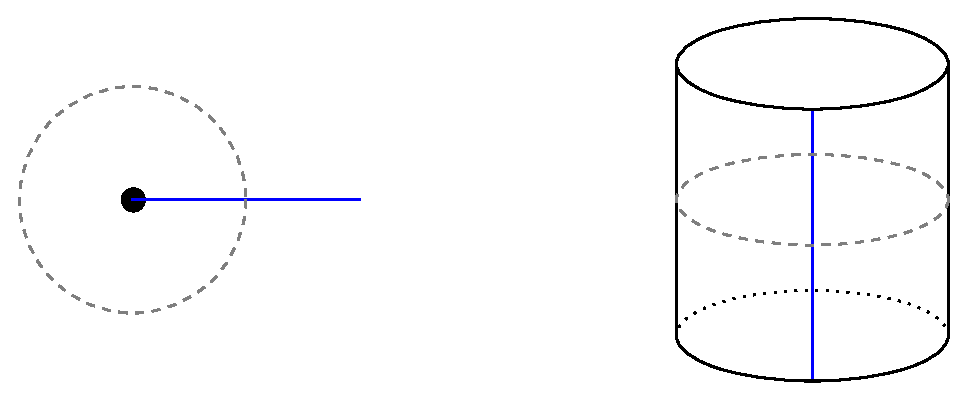
\includegraphics[width=.6\textwidth]{figures/defectop.pdf}
\caption{Left: a defect operator (black dot) attached to a topological defect line ${\cal L}$ (blue). Right: the corresponding state on the cylinder in the presence of the defect (blue, extended in time).}\label{fig:defectop}
\end{figure}

Given two topological lines ${\cal L}_1$ and ${\cal L}_2$, one can construct their direct sum ${\cal L}_1\oplus {\cal L}_2$, which obeys ${\cal H}_{{\cal L}_1\oplus {\cal L}_2} = {\cal H}_{{\cal L}_1} \oplus {\cal H}_{{\cal L}_2}$. Topological defect lines that cannot be reduced to a direct sum will be referred to as ``simple". One can also fuse a pair of topological lines ${\cal L}_1$ and ${\cal L}_2$, by bringing them next to each other, which results in a new topological line ${\cal L}_1\triangleright{\cal L}_2$. The fusion operation is associative but need not be commutative. The fusion of simple topological lines can be decomposed into a direct sum, via
\ie\label{lllfuse}
{\cal L}_i \triangleright{\cal L}_j = \bigoplus_k N_{ij}^k {\cal L}_k,
\fe
where $N_{ij}^k$ are non-negative integers and represent the number of copies of ${\cal L}_k$ in the direct summand.

The possibility of fusion also means that topological lines can form junctions. A junction of three (ordered) topological lines ${\cal L}_1, {\cal L}_2, {\cal L}_3$ is itself a (topological) defect operator; such operators span a vector space $V_{{\cal L}_1{\cal L}_2{\cal L}_3}$, which is the subspace of weight $(0,0)$ states in ${\cal H}_{{\cal L}_1 \triangleright{\cal L}_2\triangleright{\cal L}_3}$. For simple lines ${\cal L}_i$, ${\rm dim} V_{{\cal L}_i{\cal L}_j{\cal L}_k}$ is equal to the fusion coefficients $N_{ij}^{\overline k}$, where ${\cal L}_{\overline k}$ is the orientation reversal of ${\cal L}_k$.

Given a pair of junctions operators in $V_{{\cal L}_i {\cal L}_j{\cal L}_m}$ and $V_{{\cal L}_k {\cal L}_\ell{\cal L}_{\overline m}}$, we can form a 4-way ``H-junction" by connecting the ${\cal L}_m$ line with ${\cal L}_{\overline m}$. The H-junction operator can be expressed in a cross-channel as a state in $\bigoplus_n V_{{\cal L}_j {\cal L}_k{\cal L}_n}\otimes V_{{\cal L}_\ell {\cal L}_i {\cal L}_{\overline n}}$. This defines a linear map
\ie\label{hcrossk}
K_{ij}^{\ell k}: ~\bigoplus_m V_{{\cal L}_i {\cal L}_j{\cal L}_m}\otimes V_{{\cal L}_k {\cal L}_\ell{\cal L}_{\overline m}}
\to \bigoplus_n V_{{\cal L}_j {\cal L}_k{\cal L}_n}\otimes V_{{\cal L}_\ell {\cal L}_i {\cal L}_{\overline n}},
\fe
which we refer to as the H-junction crossing kernel. The $K_{ij}^{\ell k}$'s obey a set of consistency relations that follow from a sequence of H-junction crossing moves on a 5-way junction, known as the pentagon identity. 

A basic class of topological defect lines are ``symmetry lines" or ``invertible lines", which are associated with symmetries of the CFT. Let $G$ be the symmetry group, it is expected that every element $g\in G$ comes with a simple topological line ${\cal L}_g$, such that the fusion is governed by group product, namely ${\cal L}_{g_1}\triangleright{\cal L}_{g_2} = {\cal L}_{g_1 g_2}$. This is a special case of (\ref{lllfuse}) where only one of the fusion coefficients is nonzero (and is equal to 1). The junction operator space $V_{{\cal L}_{g_1} {\cal L}_{g_2} {\cal L}_{g_3}}$ is isomorphic to $\mathbb{C}$ when $g_1g_2g_3=1$, and trivial otherwise. We can pick a basis vector $v_{g_1 , g_2}\in V_{{\cal L}_{g_1} {\cal L}_{g_2} {\cal L}_{(g_1g_2)^{-1}}}$ for each junction, and express the crossing kernel (\ref{hcrossk}) as
\ie\label{crossingphase}
K_{g_1, g_2}^{(g_1g_2g_3)^{-1}, g_3} (v_{g_1 ,g_2}\otimes v_{g_3, (g_1g_2g_3)^{-1}}) = e^{i\theta(g_1, g_2, g_3)} (v_{g_2, g_3}\otimes v_{(g_1 g_2 g_3)^{-1}, g_1}).
\fe
The pentagon identity implies the following relation of the crossing phase $\theta$,
\ie\label{pentatheta}
\theta(g_1, g_2, g_3 g_4) + \theta( g_1 g_2, g_3, g_4) = \theta(g_2, g_3, g_4) + \theta(g_1, g_2g_3, g_4) + \theta(g_1, g_2, g_3).
\fe
On the other hand, if we rotate the phase of the basis vector $v_{g_1, g_2}$ by $e^{i\varphi(g_1, g_2)}$, $\theta$ changes by
\ie\label{pharthetshif}
\delta\theta(g_1 ,g_2, g_3) = \varphi(g_1, g_2) +\varphi(g_1, g_2g_3) - \varphi(g_1g_2, g_3) - \varphi(g_1, g_2).
\fe
The set of possible crossing phases $\theta$ that obey the consistency condition (\ref{pentatheta}) modulo the ambiguity (\ref{pharthetshif}) defines the group cohomology $H^3(G, U(1))$. If the $G$-symmetry lines in a CFT have crossing phases that represent a nontrivial class in $H^3(G, U(1))$, we say that the symmetry is subject to 't Hooft anomaly. A consequence of the 't Hooft anomaly will be discussed in section \ref{orbifoldsection}.

The Ising CFT admits a $\mathbb{Z}_2$ symmetry $\widehat\eta$ that flips the sign of the spin field $\sigma$ while leaving the energy operator $\varepsilon$ invariant. We will denote the associated symmetry line $\eta$. It follows from the modular property
\ie
{\rm Tr}_{\cal H} \widehat{\eta} e^{-{2\pi i\over \tau} (L_0-{c\over 24})}\bar q^{{2\pi i\over \bar\tau} (\widetilde L_0-{c\over 24})} = {\rm Tr}_{{\cal H}_{\eta}} e^{{2\pi i \tau} (L_0-{c\over 24})}\bar q^{-{2\pi i \bar\tau} (\widetilde L_0-{c\over 24})}
\fe
that ${\cal H}_\eta$ contains Virasoro primaries $\psi$, $\widetilde\psi$, $\mu$, of weight $({1\over 2}, 0)$, $(0,{1\over 2})$, and $({1\over 16},{1\over 16})$ respectively. $\psi$ and $\widetilde\psi$ are the free fermion fields, which we now recognize as defect operators. $\mu$ is called the disorder operator. Note that the OPE of $\psi$ or $\widetilde\psi$ with $\sigma$ contains $\mu$. Up to a phase convention of the states and a sign convention for the fermion field, we have $\psi_0 |\sigma\rangle = i \widetilde\psi_0|\sigma\rangle = {1\over \sqrt{2}}|\mu\rangle$.\footnote{The relative factor of $i$ between $\psi_0|\sigma\rangle$ and $\wt\psi_0|\sigma\rangle$ is necessary for consistency with $\{\psi_0, \wt\psi_0\}=0$ and $\psi_0^2=\wt\psi_0^2={1\over 2}$. }

The Ising CFT also admits a non-invertible topological defect line, known as duality defect, denoted by ${\cal N}$. Let $\widehat{\cal N}$ be the operator defined by a spatial ${\cal N}$ loop on the cylinder, we then have
\ie\label{nhatdef}
\widehat{\cal N} |1\rangle = \sqrt{2} |1\rangle,~~~ \widehat{\cal N} |\varepsilon\rangle = -\sqrt{2} |\varepsilon\rangle,~~~
\widehat{\cal N}|\sigma\rangle = 0.
\fe
${\cal N}$ obeys the fusion relation
\ie
{\cal N}^2\equiv {\cal N}\triangleright {\cal N} = I + \eta,
\fe
where $I$ stands for the trivial line and $\eta$ the $\mathbb{Z}_2$ symmetry line. It follows from (\ref{nhatdef}) and the modular property of the torus character that ${\cal H}_{\cal N}$ contains Virasoro primaries of weight $({1\over 16},0)$, $({1\over 16}, {1\over 2})$, $(0,{1\over 16})$, and $({1\over 2}, {1\over 16})$. Using the fusion and crossing relations, one can show that ``lassoing" the spin field $\sigma$ by an ${\cal N}$ line produces the disorder operator $\mu$ (which is attached to an $\eta$ line).



\subsection{Orbifolds}
\label{orbifoldsection}

If a CFT $M$ admits a discrete symmetry group $G$ that is free of 't Hooft anomaly, it is then possible to gauge $G$ to produce a new CFT, known as the orbifold CFT, denoted by $M/G$. We begin with the Hilbert space ${\cal H}_g$ of defect operators attached to the symmetry line ${\cal L}_g$, for an element $g\in G$. In the absence of 't Hooft anomaly, the crossing phase $\theta(g_1, g_2, g_3)$ in (\ref{crossingphase}) can be removed via (\ref{pharthetshif}) by choosing a (not necessarily unique) set of junction vectors, and so the 4-way junction of ${\cal L}_h$, ${\cal L}_g$, ${\cal L}_{h^{-1}}$, ${\cal L}_{hg^{-1}h^{-1}}$ can be consistently defined by splitting into a pair of 3-way junctions. This allows for defining the action of the symmetry group element $h$,
\ie
\widehat h: ~{\cal H}_g \to {\cal H}_{h g h^{-1}}
\fe 
by encircling the defect operator with an ${\cal L}_h$ loop. % as in \fixme{Figure}.

\begin{figure}[h!]
\centering
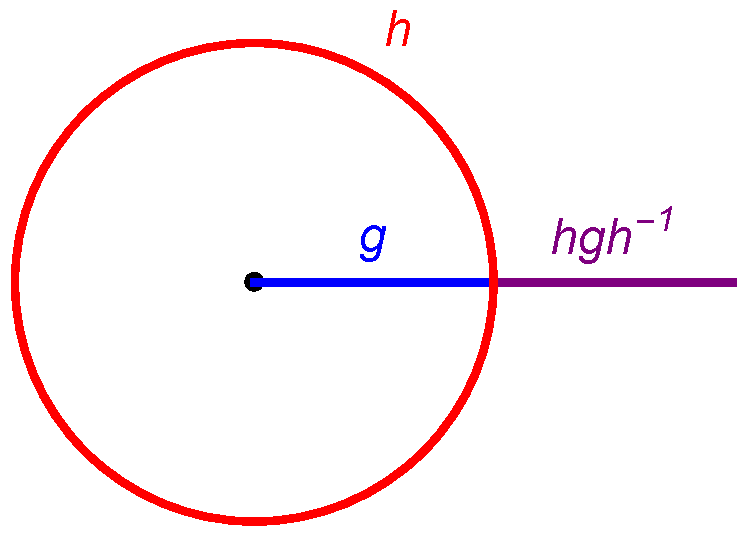
\includegraphics[width=.25\textwidth]{figures/defectsym.pdf}
\caption{The action of $\widehat h$ on a defect operator (black dot) in ${\cal H}_g$, realized by encircling with ${\cal L}_h$ (red) and a 4-way junction.}\label{fig:defectsym}
\end{figure}

The Hilbert space of $M/G$, denoted by ${\cal H}_{M/G}$, will be constructed as the $G$-invariant subspace of $\bigoplus_{g\in G} {\cal H}_g$. %We can also write
%\ie
%{\cal H}_{M/G} \simeq \bigoplus_{{\rm conjugacy~class}~[g]} ({\cal H}_g)^{Z_g},
%\fe
%where $Z_g$ is the commutant of $g$ in $G$, and $({\cal H}_g)^{Z_g}$ is the $Z_g$-invariant subspace of ${\cal H}_g$. 
This is such that ${\cal L}_g$ can be freely moved past an operator in ${\cal H}_{M/G}$, and so the correlation functions of operators in ${\cal H}_{M/G}$, a priori defined as correlators of defect operators in $M$, behave like those of local operators in a CFT. Modular invariance is manifest in this construction. For instance, the torus partition function of $M/G$ can be written as
\ie
& Z_{M/G}(\tau,\bar\tau) = \sum_{{\rm conjugacy~class}~[g]} {1\over |C_g|} \sum_{h\in C_g} Z_g^h(\tau,\bar\tau),
\fe
where $C_g$ is the commutant of $g$ in $G$, and 
\ie
&Z_g^h(\tau,\bar\tau) = {\rm Tr}_{{\cal H}_g} \widehat h q^{L_0 - {c\over 24}} \bar q^{\widetilde L_0 - {\widetilde c\over 24}},
\fe
is the torus partition function with ${\cal L}_{g}$ wrapping the spatial circle and ${\cal L}_{h}$ wrapping the Euclidean time circle. The ${\cal L}_{g}$ and ${\cal L}_{h}$ loops intersect at a 4-way junction, which exists when $g$ and $h$ commute.


The orbifold construction described above is subject to an ambiguity: the choice of 3-way junction vectors that trivialize the crossing phases (in the absence of 't Hooft anomaly) may not be unique. In particular, we may rotate the junction vector in $V_{{\cal L}_{g_1}{\cal L}_{g_2}{\cal L}_{(g_1g_2)^{-1}}}$ by a phase $e^{i\A(g_1, g_2)}$, subject to
\ie\label{aggdisct}
\A(g_2, g_3) + \A(g_1, g_2 g_3) - \A(g_1g_2, g_3) - \A(g_1, g_2) = 0
\fe
and the Hermiticity condition $\A(g_1^{-1},g_2^{-1}) = -\A(g_2, g_1)$, so that the 4-way junctions are still well-defined. On the other hand, the 4-way junction would be unaffected if we change $\A$ by
\ie\label{aggequp}
\delta \A(g_1, g_2) = \B(g_2) - \B(g_1g_2)+\B(g_1),
\fe
where $\B$ obeys $\B(g^{-1})=-\B(g)$. The equivalence classes of phases $\A(g_1, g_2)$ that obey (\ref{aggdisct}) modulo (\ref{aggequp}) defines the group cohomology $H^2(G,U(1))$. This is known as discrete torsion, which labels inequivalent orbifold theories based on gauging the same symmetry group $G$.


As a basic example, consider the $\mathbb{Z}_2$ symmetry of the free boson CFT, whose nontrivial element $g$ acts by flipping the sign of the field $X$. $\widehat g$ acts on an oscillator state by
\ie
\widehat g: ~\prod_i \A_{-n_i}\prod_j\widetilde\A_{-m_j} |0; k\rangle\mapsto (-)^{\sum_i n_i+\sum_j m_j} \prod_i \A_{-n_i}\prod_j\widetilde\A_{-m_j} |0; -k\rangle.
\fe
The spectrum of defect operators in ${\cal H}_g$ can be determined from modular invariance:
\ie
Z_{{\cal H}_g}(\tau,\bar\tau) \equiv Z_g^1(\tau,\bar\tau) = Z_1^g(-{1\over\tau}, -{1\over \bar\tau}),
\fe
where $Z_1^g$ is the torus character
\ie
Z_1^g(\tau, \bar\tau) = {\rm Tr} \widehat g q^{L_0 - {1\over 24}} \bar q^{\widetilde L_0 - {1\over 24}} = \left| q^{-{1\over 24}} \prod_{n=1}^\infty {1\over 1+ q^n} \right|^2.
\fe
Note that while the partition function of the free boson CFT is divergent, $Z_1^g$ is finite as it only receives contribution from $k=0$ states. Modular transformation then gives
\ie
Z_g^1(\tau,\bar\tau) = \left| q^{1\over 48} \prod_{n=0}^\infty {1\over 1- q^{n+{1\over 2}}} \right|^2.
\fe
Next, we can obtain $Z_g^g$ by performing the modular transformation $\tau\mapsto \tau+1$ on $Z_g^1$, giving
\ie
Z_g^g(\tau,\bar\tau) = \left| q^{1\over 48} \prod_{n=0}^\infty {1\over 1+ q^{n+{1\over 2}}} \right|^2.
\fe
Note that $Z_g^1$ is invariant under $\tau\mapsto \tau+2$, as is required by $g^2=1$ and the absence of 't Hooft anomaly. 

From the ``twisted sector" partition function ${1\over 2} \left( Z_g^1+Z_g^g \right)$, we see that the twisted sector ground state corresponds to an operator $\sigma$ of weight $({1\over 16},{1\over 16})$. In the orbifold CFT, the original boson field $X$ is no longer a local operator. In particular, moving $X(z,\bar z)$ around $\sigma(0)$ (or any other operator in the twisted sector) changes the former to $-X(z,\bar z)$. It is instructive to consider the 4-point function
\ie\label{fourpointratio}
{\left\langle \sigma(z,\bar z) \sigma(0) \partial X(w_1) \partial X(w_2) \right\rangle \over \left\langle \sigma(z,\bar z) \sigma(0) \right\rangle} = {P(w_1, w_2, z)\over w_{12}^2 \sqrt{w_1(w_1-z) w_2(w_2-z)}},
\fe
where $P(w_1, w_2, z)$ is a polynomial function that is at most linear in $w_1$ or in $w_2$, as is required by the fall off behavior of the LHS in the limit $w_1\to \infty$ or $w_2\to \infty$. On the other hand, in the $w_1\to w_2$ limit, the LHS behaves as $-{1\over w_{12}^2} + {\cal O}(1)$, as follows from the $\partial X(w_1) \partial X(w_2)$ OPE. This fixes $P(w_1, w_2, z) = {z(w_1+w_2)\over 2} - w_1 w_2$. Now expanding both sides of (\ref{fourpointratio}) to order 1, one finds
\ie\label{sigmatwistwei}
{\left\langle \sigma(z,\bar z)  \sigma(0)(-2T(w_2)) \right\rangle \over \left\langle \sigma(z,\bar z) \sigma(0) \right\rangle} = -{z^2\over 8 w_2^2 (w_2-z)^2},
\fe
which is precisely consistent with the weight of $\sigma$ being $h={1\over 16}$.

Generalizing this example, let us consider the orbifold of a complex free boson $Z$ by the discrete $\mathbb{Z}_N$ rotation symmetry generated by
\ie
g: ~Z\mapsto e^{2\pi i \A} Z,~~~ \overline Z \mapsto e^{-2\pi i \A} \overline Z,
\fe
where $\A = {1\over N}$.
Let $\sigma$ be the twist field corresponding to the ground state of the $g$-twisted sector, and its Hermitian conjugate $\overline\sigma$ corresponding to the ground state of the $g^{-1}$-twisted sector. We have, analogously to (\ref{fourpointratio}), 
\ie\label{fourpointratiozzbar}
{\left\langle \sigma(z,\bar z) \overline\sigma(0) \partial Z(w_1) \partial \overline Z(w_2) \right\rangle \over \left\langle \sigma(z,\bar z) \overline\sigma(0) \right\rangle} = {P(w_1, w_2, z)\over w_{12}^2 w_1^\A (w_1-z)^{1-\A} w_2^\A(w_2-z)^{1-\A}},
\fe
$P$ is again a polynomial that is at most linear in $w_1$ or in $w_2$. The leading singularity in the $w_1\to w_2$ determines $P = 2\A z w_1 + 2 (1-\A) z w_2 -2 w_1 w_2$. Expanding both sides of (\ref{fourpointratiozzbar}) to order $w_{12}^0$, we determine the weight of $\sigma$ to be $h= {\A(1-\A)\over 2}$.

\subsection{Narain lattice}
\label{naraincocyclesec}

Let $X_L^i$ ($i=1,\cdots, n_L$) be a set of holomorphic free boson fields, with the OPE
\ie
X_L^i(z) X_L^j(0) \sim - \delta^{ij} \log z,
\fe 
and $X_R^{i'}$ ($i'=1,\cdots, n_R$) a set of anti-holomorphic boson fields. The Narain lattice CFT is defined by including all operators constructed out of normal order products of $\partial^n X_L^i$, $\partial^m X_R^{i'}$, and the exponential operators 
\ie
{\cal O}_{k} = \,:e^{i k_L\cdot X_L+ i k_R\cdot X_R}:,
\fe
for vectors $k\equiv (k_L, k_R)$ in a lattice $\Gamma \subset \mathbb{R}^{n_L, n_R}$. The operators ${\cal O}_k$ and ${\cal O}_{k'}$ have single-valued OPE provided that
\ie
k\circ k' \equiv k_L\cdot k_L' - k_R \cdot k_R' \in \mathbb{Z}.
\fe
This amounts to saying that $\Gamma$ is an integral lattice with respect to the pairing induced by the inner product on $\mathbb{R}^{n_L, n_R}$. ${\cal O}_k$ has integer spin if
\ie
k\circ k \in 2 \mathbb{Z}.
\fe
This condition amounts to saying that $\Gamma$ is an {\it even} lattice. Finally, demanding that the torus partition function is modular invariant, namely
\ie
Z(\tau,\bar\tau) = {1\over (\eta(\tau))^{n_L} (\overline{\eta(\tau)})^{n_R}} \sum_{k\in \Gamma} q^{k_L^2\over 2}\bar q^{k_R^2\over 2} = Z(-1/\tau, -1/\bar\tau),
\fe
requires that $\Gamma$ is a self-dual lattice, namely $\Gamma=\Gamma^*$, where
\ie
\Gamma^* \equiv \{\ell \in \mathbb{R}^{n_L, n_R}| \ell\circ k \in \mathbb{Z}, ~\forall k \in \Gamma\}.
\fe
The self-duality condition is equivalent to saying that $\Gamma$ is {\it unimodular}, that is, given any integral basis $\{e_i\}_{i=1,\cdots, n_L+n_R}$, the matrix $(A_{ij}) = (e_i\circ e_j)$ has determinant $\pm 1$. One can further show that when this condition is satisfied, the torus 1-point function of a general primary in the Narain lattice CFT is modular covariant.

A standard theorem\footnote{See chapter 5 of Serre, {\it A Course in Arithmetic}, GTM vol. 7 \cite{serre2012course}.} asserts that such $\Gamma$ exists only when $n_L - n_R \equiv 0$ mod 8. Furthermore, if both $n_L, n_R$ are positive, the integral pairing $(A_{ij})$ is unique up to a change of basis, i.e. as an integral lattice $\Gamma$ is unique up to isomorphism (but it admits a family of inequivalent embeddings into $\mathbb{R}^{n_L, n_R}$). 

If either $n_L$ or $n_R$ is zero, on the other hand, the classification of even unimodular lattices is more intricate. For instance, if $(n_L, n_R)=(8,0)$, there is a unique such lattice $\Gamma_8$ that is the root lattice of $E_8$, with
\ie
(A_{ij}) = \begin{pmatrix} 2 & -1 & 0 & 0 & 0 & 0 & 0 & 0 \\ -1 & 2 & -1 & 0 & 0 & 0 & 0 & 0 \\ 0 & -1 & 2 & -1 & 0 & 0 & 0 & 0 \\ 0 & 0 & -1 & 2 & -1 & 0 & 0 & 0 \\ 0 & 0 & 0 & -1 & 2 & -1 & 0 & -1  \\ 0 & 0 & 0 & 0 & -1 & 2 & -1 & 0 \\ 0 & 0 & 0 & 0 & 0 & -1 & 2 & 0 \\ 0 & 0 & 0 & 0 & -1 & 0 & 0 & 2 \end{pmatrix}.
\fe
We can also represent $\Gamma_8$ through its embedding in $\mathbb{R}^8$, as the set of vectors
\ie\label{gameight}
\Gamma_8 = \left\{(n_1, \cdots, n_8)\bigg| \sum_{i=1}^8 n_i \in 2 \mathbb{Z}\right\}\cup \left\{(n_1+{1\over 2}, \cdots, n_8+{1\over 2})\bigg| \sum_{i=1}^8 n_i \in 2 \mathbb{Z}\right\}. 
\fe
If $(n_L, n_R)=(16,0)$, there are two inequivalent such lattices, $\Gamma_8\oplus \Gamma_8$ and 
\ie\label{gamsixteen}
\Gamma_{16} = \left\{(n_1, \cdots, n_{16})\bigg| \sum_{i=1}^{16} n_i \in 2 \mathbb{Z}\right\}\cup \left\{(n_1+{1\over 2}, \cdots, n_{16}+{1\over 2})\bigg| \sum_{i=1}^{16} n_i \in 2 \mathbb{Z}\right\}. 
\fe 
Note that the Narain lattice CFTs based on $\Gamma_8\oplus \Gamma_8$ and $\Gamma_{16}$ have identical torus partition functions, hence identical operator weight spectra, but different structure constants.

Let us inspect in more detail the OPE
\ie
{\cal O}_k(z, \bar z) {\cal O}_{k'}(0) \sim \epsilon(k,k') z^{k_L\cdot k_L'} \bar z^{k_R\cdot k_R'} {\cal O}_{k+k'}(0) + \cdots
\fe
where $\epsilon(k,k')$ is a constant phase factor that depends on the regularization scheme used in defining ${\cal O}_k$. It is not possible to set $\epsilon(k,k')$ to 1 for all $k,k'$, for the consistency with exchanging  ${\cal O}_k$ with ${\cal O}_{k'}$ in the OPE requires 
\ie
\epsilon(k', k) = (-)^{k\circ k'} \epsilon(k,k').
\fe 
Further, associativity of the OPE requires
\ie
\epsilon(k_1, k_2+k_3) \epsilon(k_2, k_3) = \epsilon(k_1, k_2) \epsilon(k_1+k_2, k_3).
\fe
Such a set of $\epsilon(k, k')$ is known as a 2-cocycle of the Narain lattice. Explicitly, picking an integral basis $e_i$ of $\Gamma$ and writing $k=\sum m^i e_i$, $k' = \sum n^i e_i$, a consistent choice of the cocycle $\epsilon$ is given by
\ie
\epsilon(k,k') = (-)^{\sum_{i>j} A_{ij} m^i n^j}.
\fe


\newpage

\section{Lagrangian description of 2D CFTs}






%\newpage
%
%\section{More on nonlinear sigma models}


\subsection{Weyl anomaly in the nonlinear sigma model}
\label{sec:nlsms}

To quantize the nonlinear sigma model based on the action (\ref{curvact}) in a manner that respects general coordinate invariance in the target spacetime, we will employ dimensional regularization by formally working in $2-\epsilon$ dimensions, and replace $G_{\mu\nu}(X)$, $B_{\mu\nu}(X)$, $\Phi(X)$ in  (\ref{curvact}) by the bare couplings, which we denote by $G_{\mu\nu}^\epsilon(X)$, $B_{\mu\nu}^\epsilon(X)$, $\Phi^\epsilon(X)$. The bare couplings are generally divergent in the $\epsilon\to 0$ limit. The corresponding ``physical" or ``renormalized" couplings $G_{\mu\nu}, B_{\mu\nu}, \Phi$, which are finite and dependent on a renormalization mass scale $\mu$, will be defined in the {\it minimal subtraction} scheme. That is, the bare coupling when expressed as a function of the physical couplings involves an expansion in negative powers of $\epsilon$, but no positive powers of $\epsilon$. 

Focusing on $G_{\mu\nu}$ for the moment, the relation between the bare and physical coupling takes the form
\ie\label{gmuexp}
& G^\epsilon_{\mu\nu} = \mu^{-\epsilon} \left[ G_{\mu\nu} + \sum_{n\geq 1} {1\over \epsilon^n} K^{(n)}_{\mu\nu} \right],
\fe
where $\mu$ is the renormalization scale. The coefficients $K_{\mu\nu}^{(n)}$ of negative powers of $\epsilon$, also known as ``counter terms", are functionals of $G_{\mu\nu}$ with no further, explicit, $\mu$-dependence. The bare coupling $G_{\mu\nu}^\epsilon$ by definition is independent of $\mu$. Differentiating (\ref{gmuexp}) with respect to $\log\mu$ then gives the equations
\ie\label{betaeqngst}
0\equiv \mu^\epsilon {d G_{\mu\nu}^\epsilon\over d \log\mu} = -\epsilon (G_{\mu\nu} + \sum_{n\geq 1} \epsilon^{-n} K_{\mu\nu}^{(n)}) + {dG_{\mu\nu}\over d\log\mu} + \sum_{n\geq 1} \epsilon^{-n} \int dX {dG_{\rho\sigma}(X)\over d\log\mu} {\delta K_{\mu\nu}^{(n)}\over \delta G_{\rho\sigma}(X)}.
\fe
The $\mu$-dependence of the renormalized coupling should admit an expansion in non-negative powers of $\epsilon$, that is,
\ie\label{gbetafn}
{dG_{\mu\nu}\over d \log\mu} = \sum_{m\geq 0} \epsilon^m \B_{\mu\nu}^{G(m)}.
\fe
Plugging this into (\ref{betaeqngst}) and expanding order by order in $\epsilon$, one finds that the RHS of (\ref{gbetafn}) terminates at order $\epsilon$:
\ie{}
& \B_{\mu\nu}^{G(m)} = 0,~~~m\geq 2,
\\
&  \B_{\mu\nu}^{G(1)} = \epsilon G_{\mu\nu}.
\fe
Furthermore, $\B_{\mu\nu}^{G(0)}$ obeys
\ie\label{ggrgeq}
&% {d G_{\mu\nu}\over d \log\mu} = \epsilon G_{\mu\nu} + \B^G_{\mu\nu},~~~~
 \B^{G(0)}_{\mu\nu} = \left( 1 - G {\partial\over \partial G}\right) K_{\mu\nu}^{(1)},
\\
& \B^{G(0)}{\partial\over \partial G} K^{(n)}_{\mu\nu} = \left( 1 - G {\partial\over \partial G}\right) K_{\mu\nu}^{(n+1)},
\fe
where $G {\partial\over \partial G}$ is a shorthand notation for $\int dX G_{\mu\nu}(X) {\delta\over \delta G_{\mu\nu}(X)}$, and similarly for $\B^{G(0)} {\partial\over \partial G}$. 
Since each extra power of $G_{\mu\nu}$ (or spacetime derivatives of $G_{\mu\nu}$) in $K_{\mu\nu}^{(n)}$ comes with an inverse power of $\A'$, we may also replace $1-G{\partial\over G}$ in (\ref{ggrgeq}) by $\A' {\partial\over \partial \A'}$. As a general feature of the minimal subtraction scheme, the beta function (\ref{gbetafn}) is determined entirely by the order $1/\epsilon$ counter term.

These relations can be generalized to include $B_{\mu\nu},\Phi$ and their beta functions $\B^B_{\mu\nu},\B^\Phi$. Note that the dimensional regularization of $B_{\mu\nu}$ coupling is subtle, due to the ambiguity that arises in defining the anti-symmetric tensor $\epsilon^{ab}$ in $2-\epsilon$ dimensions. Firstly, we shall replace $\epsilon^{ab}$ in (\ref{curvact}) by
\ie
e^{ab} \equiv \sqrt{g} e_i{}^a e_j{}^b \epsilon^{ij},
\fe
where $e_i{}^a$ is the inverse matrix of the frame variable $e^i{}_a$ defined via $g_{ab} = \delta_{ij} e^i{}_a e^j{}_b$. $\epsilon^{ij}$ is formally a constant anti-symmetric tensor in $2-\epsilon$ dimensions that obeys $\epsilon^{ij} \epsilon^{k\ell} = f(\epsilon) (\delta^{ik} \delta^{j\ell} - \delta^{i\ell}\delta^{jk})$, for some $f(\epsilon) = 1 + {\cal O}(\epsilon)$. The precise dimensional regularization scheme will depend on the choice of the function $f(\epsilon)$, which will affect the beta function/Weyl anomaly involving $B$-field starting at 2-loop order in the $\A'$ expansion.

The Weyl anomaly can be computed from the trace of the stress-energy tensor as derived from the bare action in $2-\epsilon$ dimensions, 
\ie\label{taatra}
2\A' T^a{}_a = \epsilon G^\epsilon_{\mu\nu} \partial^a X^\mu \partial_a X^\nu + \epsilon {ie^{ab}\over \sqrt{g}} B^\epsilon_{\mu\nu} \partial_a X^\mu \partial_b X^\nu + {\epsilon} \A'  R(g) \Phi^\epsilon(X) + 2\A' \nabla^2 \Phi^\epsilon(X).
\fe
We would like to express the RHS in terms of physical couplings and renormalized operators, the latter defined as follows. Suppose the general bare action is written in the form 
\ie
S = \int d^{2-\epsilon}\sigma\, \lambda_I^\epsilon(\sigma) {\cal O}_I(\sigma),
\fe
where $\lambda_I^\epsilon$ are all possible bare couplings (regarded as functions of worldsheet coordinate $\sigma^a$ as well), whose corresponding physical couplings are denoted $\lambda_I$. We then {\it define} the renormalized operator $[{\cal O}_I]_R$ as
\ie{}
[{\cal O}_I]_R = {\delta S\over \delta \lambda_I}.
\fe
In practice, if we only compute the relation between the bare and physical couplings for couplings that are constant on the worldsheet, we can only determine the renormalized operators up to total derivative terms. 

For instance, it follows from (\ref{gmuexp}) and (\ref{ggrgeq}) that
\ie
\epsilon \left( 1- G {\partial\over \partial G}\right) G_{\mu\nu}^\epsilon = \B^{G(0)} {\partial\over\partial G} G_{\mu\nu}^\epsilon,
\fe
and therefore we can write
\ie{}
\epsilon G^\epsilon_{\mu\nu} \partial^a X^\mu \partial_a X^\nu%&=\mu^{-\epsilon} \left[ \B^G_{\mu\nu} + \epsilon G_{\mu\nu} + \sum_{n\geq 1} {1\over \epsilon^n} (\B+\epsilon G) {\partial\over \partial G} K^{(n)}_{\mu\nu} \right] \partial^a X^\mu \partial_a X^\nu
&= (\B^{G(0)}+\epsilon G){\partial\over \partial G} G^\epsilon_{\mu\nu}(X) \partial^a X^\mu \partial_a X^\nu
\\
&= \mu^{-\epsilon} \left[ (\beta^{G(0)}_{\mu\nu}(X) +\epsilon G_{\mu\nu}(X)) \partial^a X^\mu \partial_a X^\nu + ({\rm total~deriv} ) \right]_R.
\fe
The total derivative term is expected to take the form $\partial_a(W_{\mu}(X) \,\partial^a X^\mu)$. The full Weyl anomaly (\ref{taatra}) can be put in the form
\ie
2\A' T^a{}_a = \left[ \widehat \B^G_{\mu\nu}(X) \partial^a X^\mu \partial_a X^\nu \right]_R + {i \epsilon^{ab}\over \sqrt{g}} \left[ \widehat \B^B_{\mu\nu}(X) \partial_a X^\mu \partial_b X^\nu \right]_R + \A' R(g) \left[ \widehat \B^\Phi(X) \right]_R ,
\fe
up to ${\cal O}(\epsilon)$ terms, where $\widehat \B^G_{\mu\nu}$, $\widehat \B^B_{\mu\nu}$, $\widehat \B^\Phi$ are related to the beta functions by
\ie\label{hattedbeta}
& \widehat \B^G_{\mu\nu} = \B^G_{\mu\nu}  + \nabla_{(\mu} W_{\nu)} +2 \A' \nabla_\mu\partial_\nu \Phi,
\\
& \widehat \B^B_{\mu\nu} = \B^B_{\mu\nu} + \partial_{[\mu} L_{\nu]} + {1\over 2} H_{\mu\nu\rho} W^\rho + \A' H_{\mu\nu}{}^\rho \partial_\rho\Phi,
\\
& \widehat \B^\Phi = \B^\Phi + {1\over 2} \partial_\mu\Phi W^\mu + \A' \partial^\mu\Phi \partial_\mu \Phi ,
\fe
where $H_{\mu\nu\rho} = 3 \partial_{[\mu} B_{\nu\rho]}$, and we have omitted the superscript $(0)$ on the beta functions appearing on the RHS, with the $\epsilon\to 0$ limit understood. The appearance of $W_\mu$ in $\widehat\B^B_{\mu\nu}$ and $\widehat\B^\Phi$ comes from rewriting $W_\mu(X)\nabla^2 X^\mu$ using the equation of motion for $X^\mu$. Similarly, the last term in each line involving $\Phi$ comes from rewriting $\nabla^2\Phi$ using the equation of motion. The functions $W_\mu(X)$ and $L_\mu(X)$, coming from the total derivative terms in the renormalized operators, can be determined by the consistency conditions on the Weyl anomaly and turn out to be absent at order $\A'$.




\subsection{Some conformal nonlinear sigma models}
\label{sec:wzwcoset}

The WZW model based on group $G$ at level $k$ admits a Lagrangian description that is a nonlinear sigma model with target space metric
\ie\label{dsrmet}
ds^2 = -{R^2\over 2} {\rm tr} \left(g^{-1}dg\, g^{-1} dg\right),
\fe
where $R^2 = \A' k$, and $H$ field strength
\ie
H_3 = dB_2 = {1\over 6} {\A' k} \,{\rm tr} \left(g^{-1}d g\wedge g^{-1} d g\wedge g^{-1} dg\right).
\fe
The dilaton $\Phi$ is taken to be a constant. For instance, for $G=SU(2)$, we may represent $g$ in terms of Hopf coordinates $(\theta, \phi, \psi)$ as
\ie\label{sutwocoor}
g &= \exp\left( i {\psi+\phi\over 2}\sigma_2 \right) \exp\left(i \theta \sigma_3\right) \exp\left( i {\psi-\phi\over 2}\sigma_2 \right)
\\
&= \begin{pmatrix} \cos \psi \cos\theta + i \cos\phi \sin\theta && \sin \psi \cos\theta - i \sin\phi \sin\theta \\ -\sin \psi \cos\theta - i\sin\phi \sin\theta & & \cos\psi \cos\theta - i \cos\phi \sin\theta \end{pmatrix}.
\fe
Note that $\theta$ takes value in the range $[0,{\pi\over 2}]$, whereas $\psi,\phi$ are angular variables of periodicity $2\pi$.
The target space metric and $H$ flux for the $SU(2)_k$ WZW model can be written as
\ie\label{suwzwtargss}
& ds^2 = R^2 (d\theta^2 + \cos^2\theta d\psi^2 + \sin^2\theta d\phi^2),
\\
& H_3 = 2\A' k \cos\theta \sin\theta d\theta \wedge d\phi \wedge d\psi.
\fe
Comparing to (\ref{oneloopweyl}), we see that the 1-loop beta functions vanish, and that the central charge is given by $c = 3 - {1\over 4} \A' H_{\mu\nu\rho} H^{\mu\nu\rho} + {\cal O}(\A'^2) = 3 - {6\over k} + {\cal O}(k^{-2})$. This indeed agrees with the exact result $c={3k\over k+2}$ for the Sugawara stress-energy tensor up to higher loop corrections in $\A'$.

Next, let us consider solutions to the vanishing Weyl anomaly (up to a constant in $\widehat\B^\Phi$) condition with varying dilaton, specializing to the case of a 2-dimensional target space, where the $H$ flux is absent. The condition for Weyl invariance at 1-loop is
\ie\label{rmunuanp}
R_{\mu\nu} + 2 \nabla_\mu \partial_\nu \Phi = 0,~~~ \nabla^2\Phi - 2 (\nabla\Phi)^2 = {\rm constant}.
\fe
For the rotationally symmetric ansatz $ds^2 = e^{2\Omega(r)}(dr^2+r^2 d\phi^2)$, $\Phi = \Phi(r)$, a nontrivial solution to (\ref{rmunuanp}) is
\ie\label{phisolsa}
\Phi(r)  =  - {1\over 2} \log(1\pm r^2),~~~\Omega(r) = \Phi(r) + \log R,
\fe
where $R$ is a constant. The solution corresponding to the choice of $+$ sign in (\ref{phisolsa}), upon the change of variable $r=\sinh\rho$, can be written as
\ie\label{cigartarget}
ds^2 = R^2(d\rho^2 + \tanh^2\rho d\phi^2),~~~  \Phi(r) = -\log \cosh\rho,
\fe
where $\rho\in [0,\infty)$. The nonlinear sigma model based on this cigar-like target space geometry, with an asymptotically linear dilaton background, gives rise to the so-called cigar CFT.

The alternative choice of $-$ sign in (\ref{phisolsa}), with $r=\sin\theta$, gives rise to the ``disc'' or ``bell'' geometry
\ie\label{belltarget}
ds^2 = R^2(d\theta^2 + \tan^2\theta d\phi^2),~~~  \Phi(r) = -\log \cos\theta.
\fe
The coordinate $\theta$ ranges from 0 to ${\pi\over 2}$. Both the geometry and the dilaton appear singular at $\theta = {\pi\over 2}$. In the next section, we will construct families of exact CFTs that correspond to the nonlinear sigma models based on (\ref{cigartarget}) and (\ref{belltarget}) in the semi-classical limit.


\subsection{Buscher rules of T-duality}
\label{app:tduality}

Consider a conformal NLSM whose target space admits a $U(1)$ isometry that acts by shifting a $2\pi$-periodic angular coordinate $\psi$, with the (string frame) metric, $B$-field, and the dilaton profile
\ie{}
& ds^2 = g_{ij}(x) dx^i dx^j + 2 g_{i\psi}(x) dx^i d\psi + g_{\psi\psi}(x) d\psi^2,
\\
& B = {1\over 2} b_{ij}(x) dx^i\wedge dx^j + b_{i\psi}(x) dx^i \wedge d\psi,~~~~ \Phi = \phi(x).
\fe
The Euclidean action on a general worldsheet $\Sigma$ reads
\ie
S &= {1\over 4\pi \A'} \int_\Sigma d^2\sigma \Big[ \sqrt{g} \left( g_{ij}(x) \partial^a x^i \partial_a x^j + 2 g_{i\psi}(x) \partial^a x^i \partial_a \psi + g_{\psi\psi}(x) \partial^a \psi \partial_a \psi \right) 
\\
&~~~~ + i \epsilon^{ab} \left( b_{ij}(x) \partial_a x^i \partial_b x^j + 2 b_{i\psi}(x) \partial_a x^i \partial_b \psi \right) + \A' \sqrt{g} R(g) \phi(x) \Big].
\fe
The idea is to trade $\partial_a \psi$ with an auxiliary 1-form field $V' = V'_a(x) d\sigma^a$ that obeys the constraint $\epsilon^{ab} \partial_a V'_b = 0$, and such that the integral of $V'$ along any 1-cycle $\C$ in $\Sigma$ is an integer multiple of $2\pi$. This is implemented by rewriting the path integral as
\ie\label{tdualpathint}
\int [Dx^i D\psi] e^{-S[X,\psi]} = \int [Dx^i DV_a D\wt\psi] \,{\cal J} e^{- S' [X,V,\wt\psi]},
\fe
where
\ie
S' &= {1\over 4\pi \A'} \int_\Sigma d^2\sigma \Big[ \sqrt{g} \left( g_{ij}(x) \partial^a x^i \partial_a x^j + 2 g_{i\psi}(x) \partial^a x^i V_a + g_{\psi\psi}(x) V^a V_a \right) 
\\
&~~~~ + i \epsilon^{ab} \left( b_{ij}(x) \partial_a x^i \partial_b x^j + 2 b_{i\psi}(x) \partial_a x^i V_b \right) + 2i \A' \epsilon^{ab} \partial_a \wt\psi V_b + \A' \sqrt{g} R(g) \phi(x) \Big].
\fe
Here $V=V_a d\sigma^a$ is an unconstrained 1-form field, and the Lagrange multiplier field $\wt\psi$ is subject to the periodic identification $\wt\psi \sim \wt\psi + 2\pi$. Integrating out $\wt\psi$ then imposes the constraint that the 1-form $V$ is closed, as well as the correct quantization condition on the periods of $V$. The Jacobian factor ${\cal J}$ on the RHS of (\ref{tdualpathint}) accounts for the difference between $[D\psi]$ and the integration measure over $V$ subject to $dV=0$, and is formally
\ie\label{caljexprss}
{\cal J} = \left[ {\det \left( \nabla_a {1\over \A'} g_{\psi\psi} \nabla^a \right)\over \det\nabla^2} \right]^{1\over 2},
\fe
where $\det$ stands for the functional determinant over the space of scalar functions on $\Sigma$. A more precise regularized expression will be given in (\ref{deltdeldet}) below.

%\ie
%[D\psi] = \int [DV] \delta(dV) {\cal J} \bigg|_{V=d\psi} .
%\fe
 
On the other hand, integrating out $V_a$ on the RHS of (\ref{tdualpathint}) gives
\ie\label{tdualpathintssmd}
\int [Dx^i d\wt\psi] e^{-\wt S[X,\wt\psi]},
\fe
where
\ie\label{wtsfpri}
\wt S &= {1\over 4\pi \A'} \int_\Sigma d^2\sigma \Big[ \sqrt{g} \left( \wt g_{ij}(x) \partial^a x^i \partial_a x^j + 2 \wt g_{i\wt\psi}(x) \partial^a x^i \partial_a\wt\psi + \wt g_{\wt\psi\wt\psi}(x) \partial^a\wt\psi \partial_a\wt\psi \right) 
\\
&~~~~~~~~~~~~ + i \epsilon^{ab} \left( \wt b_{ij}(x) \partial_a x^i \partial_b x^j + 2 \wt b_{i\wt\psi}(x) \partial_a x^i \partial_b \wt\psi \right) 
+ \A' \sqrt{g} R(g) \phi(x) \Big] 
\\
&~~~~
+ {1\over 2} \log \det{}_V \left[ {1\over \A'} g_{\psi\psi}(x) \right] - \log {\cal J} + \log \wt{\cal J}.
\fe
Here $\det{}_V$ stands for the functional determinant of a linear operator acting on the space of 1-forms on $\Sigma$, and
\ie\label{tdualgbexbush}
& \wt g_{ij} = g_{ij} - {g_{i\psi} g_{j\psi} - b_{i\psi} b_{j\psi} \over g_{\psi\psi}},~~~~ 
\wt g_{i\wt\psi} = \A' {b_{i\psi} \over g_{\psi\psi}},~~~~ \wt g_{\wt\psi\wt\psi} = {\A'^2\over g_{\psi\psi}},
\\
& \wt b_{ij} = b_{ij} - {g_{i\psi} b_{j\psi} - b_{i\psi} g_{j\psi} \over g_{\psi\psi}},~~~~ \wt b_{i\wt \psi} = \A' {g_{i\psi}\over g_{\psi\psi}}.
\fe
$\wt {\cal J}$ is given by the expression (\ref{caljexprss}) with $g_{\psi\psi}$ replaced by $\wt g_{\wt\psi\wt\psi}$.

The functional determinant and the Jacobian factors appearing in the last line of (\ref{wtsfpri}) can be evaluated using the heat kernel regularization,
\ie\label{deltdeldet}
& {1\over 2} \log\det{}_V (f(x)) = {1\over 2} {\rm tr}_V \left[ \log f(x)\, e^{ - \epsilon \Delta_1 } \right],
\\
& - \log {\cal J} + \log\wt{\cal J} = {1\over 2} {\rm tr}_S \left[\left( \log (\nabla_a f(x)\nabla^a) - \log (\nabla_a {1\over f(x)}\nabla^a) \right) \, e^{ - \epsilon \Delta_0 } \right],
\fe
where ${\rm tr}_V$ and ${\rm tr}_S$ are the traces over 1-forms and scalar functions respectively. $f(x) \equiv {1\over \A'} g_{\psi\psi}(x)$ is viewed as a linear operator that acts by multiplication. $\epsilon$ is a small positive regularization parameter. $\Delta_1 = dd^* + d^*d$ is the Laplacian on 1-forms, related to the covariant derivative $\nabla$ by $(\Delta V)_a = -\nabla^2 V_a + {1\over 2} R V_a$, whereas $\Delta_0 = -\nabla^2$ is the Laplacian on scalar functions. Note that the 1-form and scalar Laplacians are paired by $\Delta_1 d = d \Delta_0$, $d^*\Delta_1 = \Delta_0 d^*$. Using the heat kernel expansion\footnote{Vassilevich, Phys. Rept. \textbf{388}, 279 (2003) \cite{Vassilevich:2003xt}.} one finds
\ie{}
{1\over 2}  \log\det{}_V (f(x)) -  \log {\cal J} + \log \wt{\cal J} 
%\\
%& = {1\over 4\pi} \int d^2\sigma \sqrt{g} \log f(x) \left[ {1\over \epsilon} + \left( {1\over 6} - {1\over 2} \right) R(g) - {1\over \epsilon} - {1\over 6} R(g) \right]
%\\
= - {1\over 8\pi}  \int d^2\sigma \sqrt{g} \log f(x) R(g).
\fe
Namely, (\ref{tdualpathintssmd}) is a NLSM with the metric $\wt g_{\mu\nu}$ and $B$-field $\wt b_{\mu\nu}$ given by (\ref{tdualgbexbush}), together with the dilaton profile
\ie\label{wtphitdual}
\wt\Phi = \phi(x) - {1\over 2} \log \left({1\over \A'} g_{\psi\psi}(x) \right).
\fe
(\ref{tdualgbexbush}) and (\ref{wtphitdual}), known as Buscher rules,\footnote{Buscher,
Phys. Lett. B \textbf{201}, 466 (1988) \cite{Buscher:1987qj}.} amount to the general form of T-duality transformation.


\subsection{Gauged WZW and coset models}
\label{sec:coset}

The $SU(2)/U(1)$ coset model may be obtained by coupling the $SU(2)_k$ WZW model (\ref{suwzwtargss}) to a $U(1)$ gauge field $(A_z, A_{\bar z})$, such that the shift symmetry in the angular coordinate $\psi$ is replaced with a gauge symmetry under which $A_a\to A_a + \partial_a \zeta$, $\psi\to \psi - \zeta$, and flowing to the IR fixed point or equivalently taking the limit of infinite gauge coupling. The action of the gauged NLSM can be put in the form
\ie
S = {k\over 2\pi} \int_{\Sigma} d^2z \left[ \partial \theta \bar\partial\theta + \tan^2\theta \partial\phi \bar\partial \phi + \cos^2\theta \left( \partial\psi + \tan^2\theta \partial\phi + A_z \right) \left( \bar\partial\psi - \tan^2\theta \bar\partial\phi + A_{\bar z} \right) \right].
\fe
It is convenient to work in the gauge where $\psi$ is set to a constant. We can then integrate out $A_a$, whose Gaussian functional determinant can be calculated as in (\ref{deltdeldet}), and produces a nontrivial dilaton profile
\ie
\Phi = - \log (k \cos\theta).
\fe
The resulting conformal NLSM, up to a constant shift of the dilaton, is precisely that of (\ref{belltarget}).

Similarly, the $SL(2,\mathbb{R})/U(1)$ coset model can be represented by the gauged WZW model with the action
\ie
S =  {k\over 2\pi} \int_{\Sigma} d^2z \left[ \partial \rho \bar\partial\rho + \tanh^2 \rho \partial\phi \bar\partial \phi - \cosh^2\rho \left( \partial t + \tanh^2\rho \partial\phi + A_z \right) \left( \bar\partial t - \tanh^2\rho \bar\partial\phi + A_{\bar z} \right) \right],
\fe
and a suitable choice of Wick-rotated integration contour in the field space. Integrating out $A_a$ then produces the dilaton profile
\ie
\Phi = - \log (k \cosh \rho),
\fe
in agreement with (\ref{cigartarget}) up to a constant shift of the dilaton.



\subsection{Liouville CFT}
\label{liouvillecftsec}

The Liouville theory is defined, at least at the semiclassical level, by the action 
\ie\label{sliouvi}
S_L[\phi] = {1\over 4\pi} \int d^2\sigma \sqrt{g} \left( g^{ab} \partial_a \phi \partial_b \phi + Q R \phi + 4\pi \mu e^{2b\phi} \right),
\fe
where $R$ is the scalar curvature of the background metric $g$. To define the quantum theory via the path integral requires specifying a regularization scheme. One approach is to view Liouville theory as a deformation of the linear dilaton CFT (section \ref{conesec}) with background charge $Q$ and central charge $c=\widetilde c = 1+6Q^2$. The operator $e^{2b\phi}$ in the linear dilaton theory (as defined by free field normal ordering) has conformal weight $h=\widetilde h = b(Q-b)$, and is marginal when 
\ie
Q=b+b^{-1}. 
\fe
With this choice of $b$, one finds that the coupling $\mu$ has vanishing beta function,\footnote{For instance, the absence of beta function at order $\mu^2$ follows from the fact that the OPE of $e^{2b\phi}$ with itself in the linear dilaton CFT does not contain any marginal primary.} indicating that the Liouville theory is in fact a CFT.

One may equivalently formulate the quantum Liouville theory via canonical quantization. This amounts to starting with the linear dilaton theory on the cylinder, whose Hamiltonian is identical to that of a free boson, and deforming the Hamiltonian by $\mu \int d\sigma \, e^{2b\phi}$ (where the operator $e^{2b\phi}$ is defined by the free field normal ordering). A generic energy eigenstate takes the form of a scattering state in the field configuration space parameterized by the Fourier modes of $\phi(\sigma) = \sum_{n\in \mathbb{Z}} \phi_n e^{in\sigma}$, whose wave functional in the asymptotic region $\phi_0 \to -\infty$ is a superposition of incoming and outgoing waves related by reflection off the Liouville potential wall. In particular, the wave functional of a typical primary state has the asymptotic form
\ie
\Psi_P^{\rm in}[\phi] \sim \left( e^{2i P \phi_0} + S(P) e^{-2i P \phi_0} \right) e^{ - \sum_{n=1}^\infty n \phi_n \phi_{-n} },~~~~ \phi_0 \to - \infty,
\fe
where the dependence on $\phi_{n\not=0}$ takes the form of the oscillator ground state of the free boson. Here $P\in \mathbb{R}_{\geq 0}$ is the target space momentum of the incoming wave, and $S(P)$ is a scattering phase. We will denote the corresponding vertex operator of the Liouville theory by $V^{\rm in}_P$. In the asymptotic region, $V^{\rm in}_P$ may be expressed as a vertex operator of the linear dilaton CFT in the form
\ie\label{lindivasy}
V^{\rm in}_{P}  \sim e^{(Q+2i P)\phi} + S(P) e^{(Q-2i P)\phi}.
\fe
The conformal weight of $V^{\rm in}_{P}$ in the Liouville theory is the same as that of the RHS of (\ref{lindivasy}) in the linear dilaton CFT, namely $h=\widetilde h = {Q^2\over 4} + P^2$. We define the normalized operator
\ie\label{vvin}
V_P \equiv S(P)^{-{1\over 2}} V_{P}^{\rm in} ,
\fe
in which the incoming and outgoing waves in the asymptotic region are on equal footing, so that their two-point functions take the form
\ie\label{vpnormvp}
\left\langle V_P(1) V_{P'}(0)\right\rangle = \pi \delta(P-P').
\fe
The structure constants will be denoted 
\ie\label{vvvcppp}
\left\langle V_{P_1} V_{P_2} V_{P_3} \right\rangle = {\cal C}(P_1, P_2, P_3).
\fe
%or equivalently $\left\langle V_{\A_1} V_{\A_2} V_{\A_3} \right\rangle = C(\A_1, \A_2, \A_3)$, with $C(\A_1, \A_2, \A_3) = \left[\prod_{i=1}^3 S(P_i)^{1\over 2} \right] {\cal C}(P_1, P_2, P_3)$, where $\A_i \equiv {Q\over 2} + i P_i$.
In the unitary Liouville theory with real $Q$ and $c\geq 1$, $V_P$ with real non-negative $P$ form the complete set of Virasoro primaries in the Hilbert space. The 4-point function of primaries admits a conformal block decomposition of the form\footnote{For explicit numerical verification of the crossing invariance of (\ref{lioufourpt}) with the DOZZ structure constants given by (\ref{dozz}), see the Mathematica notebook ``Liouville CFT.nb'' in the repository.}
\ie\label{lioufourpt}
\left\langle V_{P_1}(z,\bar z) V_{P_2}(0) V_{P_3}(1) V_{P_4}(\infty) \right\rangle = \int_0^\infty {dP\over \pi} {\cal C}(P_1, P_2, P) {\cal C}(P_3, P_4, P) \left| {\cal F}(h_1, h_2, h_3, h_4; h_P; z) \right|^2.
\fe
To proceed, we will assume that the structure constants ${\cal C}(P_1, P_2, P_3)$ can be analytically continued in $P_1, P_2, P_3$, and consider the continuation of (\ref{lioufourpt}) to complex values of $P_i$'s. The product of structure constants ${\cal C}(P_1, P_2, P) {\cal C}(P_3, P_4, P)$ may have poles in $P$ whose position depend on $P_1, P_2, P_3, P_4$.\footnote{Due to our normalization convention (\ref{vvin}), there can also be branch cuts in $P_i$ due to the $S(P_i)^{1\over 2}$ factors, but there are no such branch cuts in $P$ in the product ${\cal C}(P_1, P_2, P) {\cal C}(P_3, P_4, P)$.} When a pole crosses the $P$-integration contour, namely the positive real axis, we must either deform the contour accordingly, or equivalently retain the real integration contour but take into account the residue contribution from the pole that has crossed the contour. 

In particular, at the imaginary Liouville momentum
\ie
P_{r, s} = {i\over 2} (r b + s b^{-1}),
\fe
for some integer $r,s\geq 1$, $V_{P_{r,s}}$ has conformal weight $h_{r,s}$ (recall (\ref{hbbform})) and thereby a null Virasoro descendant at level $rs$. Demanding that the null state vanishes as an operator equation would lead to a differential equation on the 4-point function $\left\langle V_{P_{r,s}} V_{P_1}V_{P_2}V_{P_3}\right\rangle$. The solutions to such a differential equation restricts the possible conformal blocks in the 4-point function to a finite set. The interpretation from the analytic continuation of (\ref{lioufourpt}) in $P_4$ is that as $P_4$ moves from the real axis to $P_{r,s}$, a number of poles of the integrand in $P$ has crossed the contour, and the 4-point function is dominated by the contributions from these residues.

For our purpose, it will suffice to consider the continuation of $P_4$ to $P_{2,1}$. The null state condition
\ie
(L_{-1}^2 + b^2 L_{-2}) V_{P_{2,1}} = 0
\fe
leads to the second order differential equation
\ie\label{vdiffaeqgen}
\left\{ \partial_x^2 + b^2 \sum_{i=1}^3\left[ {h_i\over (x-z_i)^2 } + {1\over x-z_i} \partial_{z_i} \right] \right\} \left\langle V_{P_{2,1}}(x,\bar x) \prod_{j=1}^3 V_{P_j}(z_j,\bar z_j) \right\rangle = 0
\fe 
where $h_i = {Q^2\over 4} + P_i^2$, and the analogous anti-holomorphic differential equation. Writing
\ie\label{vvgenfrpt}
& \left\langle V_{P_{2,1}}(x,\bar x) \prod_{j=1}^3 V_{P_j}(z_j,\bar z_j) \right\rangle 
\\
& = |x-z_3|^{-4 h_{2,1}} |z_{12}|^{2(h_3-h_1-h_2-h_{2,1})} |z_{13}|^{2(h_2-h_1-h_3+h_{2,1})} |z_{23}|^{2(h_1-h_2-h_3+h_{2,1})}  f(z,\bar z),
\fe
where $z = {(x-z_1)(z_2-z_3)\over (x-z_3)(z_2-z_1)}$, it follows from (\ref{vdiffaeqgen}) that $f(z,\bar z)$ takes the form
\ie\label{fcczz}
f(z,\bar z_1) = C_+ F_+(z) F_+(\bar z) + C_- F_-(z) F_-(\bar z),
\fe
where
\ie\label{fplumin}
& F_\pm (z) = z^{{1+b^2\over 2} \pm i b P_1} (1-z)^{{1+b^2\over 2} \pm i b P_2} {}_2 F_1\left( {1\over 2} \pm ib (P_1+P_2-P_3), {1\over 2} \pm ib (P_1+P_2+P_3); 1\pm 2 ib P_1; z \right)
%\\
%& F_-(z) = z^{{1+b^2\over 2} - i b P_1} (1-z)^{{1+b^2\over 2} + i b P_2} {}_2 F_1\left( {1\over 2} - ib (P_1+P_3-P_2), {1\over 2} + ib (P_2+P_3-P_1); 1-2 ib P_1; z \right)
\fe
are conformal blocks that correspond to an intermediate primary $V_{P_1+ i {b\over 2}}$ and $V_{P_1-i{b\over 2}}$ respectively. The coefficients $C_\pm$ in (\ref{fcczz}) are related to the structure constants by
\ie\label{cpmaa}
C_\pm = 2i \, {\cal C}(P_2, P_3, P_1\pm i{b\over 2})\, {\rm Res}_{P\to P_1\pm i{b\over 2}} {\cal C}(P_1, P_{2,1}, P).
\fe
On the other hand, we can determine $C_+/C_-$ from the crossing invariance of (\ref{vvgenfrpt}). The conformal blocks in the $24\to 13$ channel can be obtained from (\ref{fplumin}) by exchanging $P_1\leftrightarrow P_2$, $z\to 1-z$. Using the property of hypergeometric function
\ie{}
& {}_2 F_1(A,B;C; 1-z) = {\Gamma(C) \Gamma(C-A-B)\over \Gamma(C-A) \Gamma(C-B)} {}_2 F_1(A,B;A+B+1-C;z) 
\\
&~~~ + {\Gamma(C)\Gamma(A+B-C)\over \Gamma(A) \Gamma(B)} z^{C-A-B}(1-z)^{1-C} {}_2 F_1(1-A,1-B; 1+C-A-B;z),
\fe
we find the crossing transformation of the conformal blocks $F_\pm$,
\ie{}
\left. \begin{pmatrix} F_+(1-z) \\ F_-(1-z) \end{pmatrix} \right|_{P_1\leftrightarrow P_2} = M \begin{pmatrix} F_+(z) \\ F_-(z) \end{pmatrix},
\fe
where $M$ is the $2\times 2$ matrix
\ie
M = \begin{pmatrix} {\Gamma(-2ib P_1) \Gamma(1+2ib P_2)\over \Gamma({1\over 2} + ib(P_2+P_3-P_1)) \Gamma({1\over 2} - ib(P_1+P_3-P_2))}  &  {\Gamma(2ib P_1) \Gamma(1+2ib P_2)\over \Gamma({1\over 2} + ib(P_1+P_2+P_3)) \Gamma({1\over 2} + ib(P_1+P_2-P_3))} \\ {\Gamma(-2ib P_1) \Gamma(1-2ib P_2)\over \Gamma({1\over 2} - ib(P_1+P_2-P_3)) \Gamma({1\over 2} - ib(P_1+P_2+P_3))}  &  {\Gamma(2ib P_1) \Gamma(1-2ib P_2)\over \Gamma({1\over 2} + ib(P_1+P_3-P_2)) \Gamma({1\over 2} - ib(P_2+P_3-P_1))} \end{pmatrix} .
\fe
Comparing the $14\to 23$ channel conformal block decomposition to the $24\to 13$ channel, we determine
\ie\label{cpmratio}
{C_+\over C_-} &=  {\gamma(-2ib P_1) \gamma({1\over 2} + i b(P_1+P_2-P_3)) \gamma({1\over 2} + i b(P_1-P_2+P_3)) \over \gamma(2ib P_1)  \gamma({1\over 2} - i b(P_1+P_2+P_3)) \gamma({1\over 2} + i b(P_2-P_1+P_3)) },
\fe
where $\gamma(x)\equiv \Gamma(x)/\Gamma(1-x)$. Further comparing (\ref{cpmaa}) in the limit $P_2\to P_1$, $P_3\to P_{2,1}$ and (\ref{cpmratio}), we find
\ie\label{refforma}
{{\rm Res}_{P\to P_1+ i{b\over 2}} {\cal C}(P_1, P_{2,1}, P)\over {\rm Res}_{P\to P_1- i{b\over 2}} {\cal C}(P_1, P_{2,1}, P)} = \left[ {\gamma(-2ib P_1) \gamma(1+b^2+2ib P_1) \over \gamma(2ib P_1) \gamma(1+b^2-2ib P_1)} \right]^{1\over 2}.
\fe
Combining (\ref{cpmaa}), (\ref{cpmratio}), (\ref{refforma}), and shifting $P_1$ to $P_1+i{b\over 2}$, we derive the relation
\ie\label{dozzrecurr}
%{{\cal C}(P_2, P_3, P_1+ i{b\over 2})\over {\cal C}(P_2, P_3, P_1- i{b\over 2})}=  \left[ {\gamma(-2ib P_1) \gamma(1+b^2-2ib P_1) \over \gamma(2ib P_1) \gamma(1+b^2+2ib P_1) } \right]^{1\over 2} {\gamma({1\over 2} + i b(P_1+P_2-P_3)) \gamma({1\over 2} + i b(P_1-P_2+P_3)) \over \gamma({1\over 2} - i b(P_1+P_2+P_3)) \gamma({1\over 2} + i b(P_2-P_1+P_3)) }.
{{\cal C}(P_2, P_3, P_1+ ib)\over {\cal C}(P_2, P_3, P_1)} &=  \left[ {\gamma(b^2-2ib P_1) \gamma(1+2b^2-2ib P_1) \over \gamma(-b^2+2ib P_1) \gamma(1+2ib P_1) } \right]^{1\over 2}
\\
&~~~\times {\gamma({1-b^2 \over 2} + i b(P_1+P_2-P_3)) \gamma({1-b^2 \over 2} + i b(P_1-P_2+P_3)) \over \gamma({1+b^2\over 2} - i b(P_1+P_2+P_3)) \gamma({1+b^2\over 2} + i b(P_2-P_1+P_3)) }.
\fe
A similar consideration of the 4-point function with a degenerate primary $V_{P_{1,2}}$ leads to an analogous relation with $b$ replaced by $1/b$. 

To construct a solution to these recursion relations, we will make use of the function $\Upsilon_b(x)$ defined by the analytic continuation of
\ie
\log\Upsilon_b(x) = \int_0^\infty {dt\over t} \left[ \left( {Q\over 2} - x \right)^2 e^{-t} - {\sinh^2\left[ ({Q\over 2}-x) {t\over 2}\right] \over \sinh{tb\over 2}\sinh{t\over 2b}} \right],~~~0<{\rm Re}(x)<Q
\fe
to the complex $x$-plane. $\Upsilon_b(x)$ is an entire analytic function with simple zeroes at $x=mb+n b^{-1}$, for integers $m,n\leq 0$ or $m,n\geq 1$. It obeys the properties
\ie{}
& \Upsilon_b(Q-x) = \Upsilon_b(x),
\\
& \Upsilon_b(x+b) = \gamma(bx) b^{1-2bx} \Upsilon_b(x),
\\
& \Upsilon_b(x+b^{-1}) = \gamma(b^{-1} x) b^{{2x\over b}-1} \Upsilon_b(x).
\fe
One then finds that
\ie\label{dozz}
{\cal C}(P_1, P_2, P_3) = {\Upsilon_b'(0) \over \Upsilon_b({Q\over 2} + i(P_1+P_2+P_3))} \prod_{j=1}^3 {\left[ \Upsilon_b(2iP_j) \Upsilon_b(-2iP_j) \right]^{1\over 2} \over \Upsilon_b({Q\over 2} + i(P_1+P_2+P_3) - 2iP_j) }
\fe
obeys the desired relations, namely (\ref{dozzrecurr}) and the analogous relation with the replacement $b\to 1/b$. Up to an overall constant factor that is independent of the Liouville momenta $P_i$, (\ref{dozz}) is the structure constant of Liouville CFT.

Note that ${\cal C}(P_1, P_2, P_3)$ has a pole at $\epsilon\equiv {Q\over 2} + i(P_1+P_2+P_3)= 0$. Near this pole, (\ref{dozz}) reduces to 
\ie
{\cal C}(P_1, P_2, P_3) \sim {1\over \epsilon} \prod_{j=1}^3 \sqrt{\Upsilon_b(2iP_j)\over \Upsilon_b(-2iP_j)}.
\fe
In this limit, the path integral computation of the Liouville structure constant is dominated by the asymptotic region $\phi\ll -{1\over 2b} \log\mu$, where the answer can be computed by the linear dilaton correlator
\ie
{\cal C}(P_1, P_2, P_3) \sim \int d\phi\, e^{-2Q\phi} \prod_{j=1}^3 S(P_j)^{-{1\over 2}} e^{(Q+2iP_j)\phi} \sim {1\over \epsilon} (\mu e^{2b\phi_0})^{-{\epsilon\over b}} \prod_{j=1}^3 S(P_j)^{-{1\over 2}},
\fe
where we have written explicitly the zero mode integral, where a factor $e^{-2Q\phi}$ is included due to the background charge, and regularized the latter by cutting off at $\phi< \phi_0 -{1\over 2b}\log \mu$, for some finite constant $\phi_0$ whose precise value will be unimportant for us. From this we determine the reflection phase
\ie\label{liouvillephase}
S(P) & = (\mu e^{2b\phi_0})^{ -{2i P\over b}} {\Upsilon_b(-2iP)\over \Upsilon_b(2iP)}
= (\mu e^{2b\phi_0} b^{2b^2-2})^{ -{2i P\over b}} {\gamma({2iP\over b})\over b^2 \gamma(-2i b P)}.
\fe








\newpage



\section{Superconformal symmetry in two dimensions}

\subsection{$(1,1)$ superspace}
\label{oneonesupers}

The free field action (\ref{freezpsiact}) can be formulated in the language of $(1,1)$ superspace on the worldsheet, by extending the coordinates $(z,\bar z)$ to include formal Grassmann-odd coordinates $(\theta, \bar\theta)$, and packaging $X^\mu$, $\psi^\mu$, $\widetilde \psi^\mu$ into a ``real superfield",
\ie\label{xsuperfield}
\mathbb{X}^\mu(z,\bar z, \theta, \bar\theta) \equiv X^\mu(z,\bar z) + i\sqrt{\A'\over 2} \theta \psi^\mu(z,\bar z) + i \sqrt{\A'\over 2} \bar\theta \widetilde\psi^\mu(z,\bar z) + \theta\bar\theta F^\mu(z,\bar z),
\fe
where $F^\mu$ will play the role of an auxiliary field that does not carry independent propagating degrees of freedom. The action (\ref{freezpsiact}) can be equivalently written as the superspace integral
\ie\label{supspcatsim}
S = {1\over 2\pi\A'} \int d^2z d^2\theta \, D_{\bar\theta} \mathbb{X}^\mu D_{\theta} \mathbb{X}_\mu ,
\fe
where $D_\theta$ and $D_{\bar\theta}$ are super-derivatives, defined as
\ie\label{superderivs}
D_\theta = \partial_\theta + \theta \partial_z,~~~ D_{\bar\theta} = \partial_{\bar\theta} + \bar\theta \partial_{\bar z}.
\fe
The super-derivatives obey the following basic relations,
\ie
D_\theta^2 = \partial_z,~~~ D_{\bar\theta}^2 = \bar\partial_{\bar z},~~~ \{D_\theta, D_{\bar\theta} \}=0.
\fe
After expanding the integrand of (\ref{supspcatsim}) in the component fields $X^\mu, \psi^\mu, \widetilde \psi^\mu, F^\mu$, and integrating out the Grassmann-odd variables $(\theta, \bar\theta)$, (\ref{supspcatsim}) reduces to (\ref{freezpsiact}) plus a quadratic term in the auxiliary fields that does not affect the dynamics. 

The action (\ref{supspcatsim}) exhibits manifest 2D $(1,1)$ super-Poincar\'e symmetry. The supersymmetry variation of the fields can be summarized as
\ie\label{susyvarbasic}
\delta_\epsilon \mathbb{X} = \left(\epsilon Q_\theta + \bar\epsilon Q_{\bar\theta}\right) \mathbb{X},
\fe
where $\epsilon$ and $\bar\epsilon$ are Grassmann-odd parameters, $Q_\theta$ and $Q_{\bar\theta}$ are defined as
\ie
Q_\theta = \partial_\theta - \theta \partial_z,~~~ Q_{\bar\theta} = \partial_{\bar\theta} - \bar\theta \partial_{\bar z}.
\fe
It is easy to see that $Q_\theta,Q_{\bar\theta}$ anti-commute with $D_\theta, D_{\bar\theta}$. Consequently, under (\ref{susyvarbasic}), the variation of the action (\ref{supspcatsim}) vanishes as it is the superspace integral of a total derivative. 


\subsection{${\cal N}=1$ superconformal algebra}
\label{sec:oneonesca}

The holomorphic ${\cal N}=1$ superconformal symmetry is generated by a stress-energy tensor $T(z)$ that obeys Virasoro algebra of central charge $c$, together with a fermionic current $G(z)$ that is a weight ${3\over 2}$ primary with respect to the Virasoro algebra. The OPE of $G(z)$ with itself takes the form
\ie\label{ggope}
G(z) G(0) \sim {2c\over 3 z^3} + {2\over z} T(0).
\fe
One of the coefficients on the RHS is fixed by the normalization convention for $G$, while the other coefficient can be fixed by applying conformal Ward identities to the correlation function $\langle G(z_1) G(z_2) T(z_3) \rangle$. Acting on any operator ${\cal O}(0)$ at the origin, we can perform the Laurent expansion of $G(z)$
\ie
G(z) = \sum_{r\in\mathbb{Z}+\nu} {G_r\over z^{r+{3\over 2}}},
\fe
where $\nu=0$ if ${\cal O}$ is in the holomorphic Ramond sector, and $\nu={1\over 2}$ if ${\cal O}$ is in the holomorphic Neveu-Schwarz sector. The new commutation relations involving the Virasoro generators $L_n$ and the superconformal generators $G_r$ are
\ie{}
& [L_n, G_r] = \left( {n\over 2} - r \right) G_{n+r},
\\
& \{ G_r, G_s\} = 2 L_{r+s} + {c\over 12} (4r^2-1) \delta_{r,-s}.
\fe
Note that in the R sector, $G_0$ and $L_0- {c\over 24} = G_0^2$ are the generators of the holomorphic part of the ${\cal N}=1$ super-Poincar\'e algebra on the cylinder.

Likewise, we can speak of the anti-holomorphic ${\cal N}=1$ superconformal algebra (SCA) generated by $\widetilde T(\bar z)$ and $\widetilde G(\bar z)$. If a CFT admits both a holomorphic and an anti-holomorphic ${\cal N}=1$ SCA, we say that it admits ${\cal N}=(1,1)$ SCA.


Similarly to how 2D conformal symmetries obey the same group relations as holomorphic coordinate transformations $z\mapsto z'(z)$, the ${\cal N}=1$ superconformal symmetry generated by $T(z)$ and $G(z)$ can be organized according to transformations of superspace coordinates $(z,\theta)\mapsto (z', \theta')$, which we refer to as ``superconformal maps", such that $D_\theta$ transforms covariantly, namely
\ie\label{ddprim}
D_\theta = (D_\theta \theta') D_{\theta'},
\fe
where $D_{\theta'} = \partial_{\theta'} + \theta' \partial_{z'}$. Let us expand
\ie{}
& z'(z,\theta) = f(z) + \theta \zeta(z),
\\
& \theta'(z, \theta) = g(z) + \theta h(z),
\fe
where $\zeta$ and $g$ are Grassmann-odd functions of $z$. $f, \zeta, g, h$ are all holomorphic in $z$, but this is not enough to satisfy (\ref{ddprim}). Indeed, by definition,
\ie
D_\theta = (D_\theta \theta') \partial_{\theta'} + (D_\theta z') \partial_{z'} = (h+\theta \partial g) \partial_{\theta'} + (\zeta + \theta \partial f) \partial_{z'}.
\fe
For the RHS to be proportional to $D_{\theta'}$, we need
\ie
\zeta + \theta \partial f = (h+\theta \partial g) \theta',
\fe
which is equivalent to
\ie
\zeta = gh, ~~~ \partial f = (\partial g) g + h^2.
\fe
Thus, we have learned that a general superconformal map takes the form
\ie\label{sctranf}
& z'(z,\theta) = f(z) + \theta g(z) h(z),
\\
& \theta'(z, \theta) = g(z) + \theta h(z),~~~ h = \pm \sqrt{\partial f + g \partial g}.
\fe
Note that while $g$ and $\partial g$ are both Grassmann-odd, $\partial f$ is invertible, and so the square root in the expression for $h(z)$ can be defined through the Taylor expansion in $g\partial g$. Such a Taylor series terminates if $g$ depends on finitely many Grassmann-odd parameters. The choice of sign or branch of the square root is important. We will see in section \ref{srssec} that this is related to the spin structure on a super Riemann surface.

The infinitesimal version of (\ref{sctranf}) takes the form %can be obtained by expanding $f(z) = z + \epsilon v(z)$, $g(z) = {1\over 2}\epsilon \eta(z)$, for a small bosonic parameter $\epsilon$. This results in the transformation
\ie\label{zthetran}
& \delta z = \epsilon \left[ v(z) + {1\over 2} \theta \eta(z)\right],
~~~~ \delta \theta = {1\over 2} \epsilon \left[ \eta(z) + \theta \partial v(z) \right],
\fe
where $\epsilon$ is a small bosonic parameter.
We can also describe the infinitesimal superconformal transformation in terms of a super vector field $\mathbb{V}(z, \theta) = v(z) + \theta \eta(z)$, via
\ie\label{infsucvec}
\delta z =\epsilon \mathbb{V} - \theta \delta \theta,~~~~ \delta \theta = {1\over 2} \epsilon D_\theta \mathbb{V}.
\fe
Under a general superconformal map $(z,\theta)\mapsto (z',\theta')$, $\mathbb{V}$ transforms into $\mathbb{V}'$, with $\epsilon\mathbb{V}' = \delta z' + \theta' \delta\theta'$. A short calculation gives
\ie\label{vvprimtran}
\mathbb{V}'(z', \theta') &= (D_\theta \theta')^2 \mathbb{V}(z,\theta).
\fe
The bosonic stress-energy tensor and the fermionic supercurrent can be organized into the super stress tensor,
\ie\label{tgrel}
\mathbb{T}(z,\theta) = {1\over 2} G(z) + \theta T(z),
\fe 
and its anti-holomorphic counterpart $\widetilde{\mathbb{T}}(\bar z, \bar\theta)$. Note that the factor ${1\over 2}$ in front of $G(z)$ on the RHS of (\ref{tgrel}) is fixed by consistency with (\ref{ggope}).
The Noether charge $-{\cal L}_{\mathbb{V}}$ that corresponds to the holomorphic superconformal symmetry generated by $\mathbb{V}$ acts on a state/operator ${\cal O}(0)$ by
\ie\label{suplv}
{\cal L}_{\mathbb{V}}\cdot {\cal O}(0)& = \oint {dz d\theta\over 2\pi i} \mathbb{V}(z,\theta) \mathbb{T}(z,\theta) {\cal O}(0)
\\
&= \oint {dz\over 2\pi i} \left[ v(z) T(z) + {1\over 2}\eta(z) G(z) \right] {\cal O}(0).
\fe
Here the superspace contour integral is defined simply as the contour integral in the bosonic variable together with the Grassmann integral in the fermionic variable.
Using either (\ref{vvprimtran}) or the OPE of supercurrents, one can compute the commutator of the superconformal charges, resulting in (\ref{strunsca}).

%The last line gives the structure constant of the ${\cal N}=1$ SCA, which will appear in the BRST transformation of the superconformal ghosts in section \ref{nsrbrstsec}.

Focusing on the holomorphic superconformal symmetry corresponding to (\ref{sctranf}), we define a superconformal primary superfield $\Phi(z, \theta)$ of weight $h$ to be one that transforms according to 
\ie\label{supconftra}
\Phi'(z',\theta') = (D_\theta \theta')^{-2h}  \Phi(z,  \theta).
\fe
Expanding
\ie\label{chisuperfiel}
\Phi(z,  \theta) = \phi(z) + \theta \chi(z) ,
\fe
it follows from (\ref{supconftra}) that $\phi$ is a conformal primary of weight $h$, whereas $\chi$ is a conformal primary of weight $h+{1\over 2}$. The infinitesimal version of (\ref{supconftra}) can be written as
\ie\label{lvsuperfield}
-{\cal L}_{\mathbb{V}} \cdot \Phi = -\left[ \mathbb{V} \partial + {1\over 2} (D_\theta \mathbb{V}) D_\theta + h \partial \mathbb{V} \right] \Phi.
\fe
Specializing to the case $\mathbb{V} = \theta \eta(z)$, $\phi$ and $\chi$ transform by
\ie
-{\cal L}_{\mathbb{V}} \cdot\phi = - {1\over 2} \eta \chi,~~~ -{\cal L}_{\mathbb{V}} \cdot \chi = - h \partial\eta \phi - {1\over 2} \eta \partial \phi .
\fe
Comparing this to (\ref{suplv}), we deduce that $\phi, \chi$ are NS sector operators that obey
\ie{}
& G_r|\phi\rangle = 0, ~~~ r \geq {1\over 2},
\\
& |\chi\rangle = G_{-{1\over 2}} |\phi\rangle.
\fe
When this is satisfied, we will refer to $\phi$ as a superconformal primary operator, and $\chi$ its level ${1\over 2}$ descendant. The anti-holomorphic versions of the superconformal primaries and their descendants are defined analogously. 

A complete basis of states in a highest weight representation of the ${\cal N}=1$ SCA can be obtained by repeatedly acting on the superconformal primary with the raising operators $G_r$ for negative $r$. All correlation functions are determined by the two-point and three-point functions of the primary {\it superfield} $\Phi(z, \theta)$, constrained by the ${\cal N}=1$ SCA to be of the following form (keeping track of only the holomorphic dependence)
\ie\label{nonetwth}
& \langle \Phi_1(z_1, \theta_1) \Phi_2(z_2, \theta_2) \rangle \propto {\delta_{h_1 h_2}\over Z_{12}^{2h_1}},
\\
& \langle \Phi_1(z_1, \theta_1) \Phi_2(z_2, \theta_2) \Phi_3(z_3, \theta_3) \rangle = {\langle \Phi_1(0, 0) \Phi_2(1, \Theta) \Phi_3'(\infty, 0) \rangle \over Z_{21}^{h_1+h_2-h_3} Z_{31}^{h_1+h_3-h_2} Z_{32}^{h_2+h_3-h_1}},
\fe
where
\ie{}
& Z_{ij} \equiv z_i - z_j - \theta_i \theta_j,
\\
& \Theta \equiv {\theta_1 z_{23} + \theta_2 z_{31} + \theta_3 z_{12} - {1\over 2} \theta_1\theta_2\theta_3 \over \sqrt{z_{12}z_{13}z_{23}}}.
\fe
Note that the three-point function appearing on the RHS of the second equation of (\ref{nonetwth}) is a linear combination of the correlator of superconformal primaries $\langle \phi_1 \phi_2 \phi_3\rangle$ and that of a descendant $\langle\phi_1 \chi_2 \phi_3\rangle$. As $\chi=G_{-{1\over 2}}\phi$ is of the opposite statistics as $\phi$, when $\langle \phi_1 \phi_2 \phi_3\rangle$ is nonzero, $\langle\phi_1 \chi_2 \phi_3\rangle$ must vanish. However, when we include the anti-holomorphic dependence, the expression analogous to the second equation (\ref{nonetwth}) would involve the correlator $\langle\phi_1 (G_{-{1\over 2}}\widetilde G_{-{1\over 2}} \phi_2) \phi_3\rangle$ which is generally nonzero and is not tied to $\langle \phi_1 \phi_2 \phi_3\rangle$ by the ${\cal N}=1$ SCA. 


\subsection{$(2,2)$ superspace}
\label{sec:twotwoss}

The two-dimensional $(2,2)$ superspace is parameterized by ordinary coordinates $(z, \bar z)$ together with the Grassmann-odd coordinates $(\theta^+, \theta^-, \overline\theta{}^+, \overline\theta{}^-)$. A chiral superfield ${\cal Z}(z,\bar z, \theta^\pm, \overline\theta{}^\pm)$ is subject to the constraint
\ie\label{dpmzconstr}
\overline D_\pm {\cal Z} = 0,
\fe
where\footnote{Our conventions for the $(2,2)$ superspace differ slightly from e.g. Witten, Nucl. Phys. B \textbf{403} (1993), 159 \cite{Witten:1993yc}. Various formulae involving the superfields are verified in the Mathematica notebook ``2D superspace.nb'' in the repository.} 
\ie{}
\overline D_+ \equiv {\partial\over \partial \overline\theta{}^+} + \theta^+ {\partial\over \partial z},~~~~ 
\overline D_- \equiv {\partial\over \partial \overline\theta{}^-} - \theta^- {\partial\over \partial \bar z}.
\fe
These constraints are solved by
\ie
{\cal Z} = Z(y, \bar y) + \theta^+ \psi_+(y, \bar y) + \theta^- \psi_-(y, \bar y) + \theta^+\theta^- F(y, \bar y), 
\fe
where
\ie
y \equiv z + \theta^+ \overline\theta{}^+,~~~~ \bar y \equiv \bar z - \theta^- \overline\theta{}^-.
\fe
Similarly, an anti-chiral superfield $\overline{\cal Z}$ is subject to the constraint
\ie
D_\pm \overline{\cal Z} = 0,
\fe
where 
\ie
D_+ \equiv {\partial\over \partial \theta^+} + \overline\theta{}^+ {\partial\over \partial z},~~~~ 
D_- \equiv {\partial\over \partial \theta{}^-} - \overline\theta{}^- {\partial\over \partial \bar z}.
\fe
The $(2,2)$ NLSM action in the superspace form (\ref{twotwoact}) can be equivalently written as
\ie\label{sactnntt}
S = - {1\over 4\pi \A'} \int d^2z\, d\theta^+ d\overline\theta{}^- \, G_{I\overline J}({\cal Z}, \overline{\cal Z}) D_- {\cal Z}^I \overline D_+ \overline{\cal Z}{}^{\overline J}. 
\fe
Note that the integrand depends on $(\overline{\theta}{}^+, \theta^-)$ only through total derivative with respect to $(z, \bar z)$. We are thus free to set $\overline\theta{}^+=\theta^+,\, \theta^-=\overline\theta{}^-$ in the integrand, and use the chiral superfield constraints to write $D_-{\cal Z}^I|_{\theta^-=\overline\theta{}^-} = (\partial_{\bar\theta^-} - 2\bar\theta^- \partial_{\bar z}) ({\cal Z}^I|_{\theta^-=\overline\theta{}^-})$, etc. Next, we can make the substitution
\ie{}
& \theta^+\to {1\over \sqrt{2}} \theta, ~~~~\overline\theta{}^-\to {i\over \sqrt{2}} \bar\theta,
\\
&{\cal Z}^I \to {\bf Z}^I(z, \bar z, \theta, \bar\theta), ~~~~ D_- {\cal Z}^I\to -i \sqrt{2} D_{\bar\theta} {\bf Z}^I, ~~~~\overline D{}_+\overline {\cal Z}{}^{\overline J} \to \sqrt{2} D_\theta {\bf Z}^{\overline J}, 
\fe
thereby reducing the action (\ref{sactnntt}) to the $(1,1)$ superspace form
\ie\label{oneonesupac}
S = {1\over \pi \A'} \int d^2z d^2\theta\, G_{I\overline J}({\bf Z},\overline{\bf Z}) D_{\bar\theta} {\bf Z}^I D_\theta \overline{\bf Z}{}^{\overline J}. 
\fe
Note that (\ref{oneonesupac}) can be equivalently written as $ {1\over \pi \A'} \int d^2z d^2\theta\, G_{I\overline J}({\bf Z},\overline{\bf Z}) D_{\bar\theta}  \overline{\bf Z}{}^{\overline J} D_\theta {\bf Z}^I$ using the K\"ahler property of the metric $G_{I\overline{J}}$ and integration by parts.

\subsection{${\cal N}=2$ superconformal algebra}
\label{sec:ntwosca}


The holomorphic ${\cal N}=2$ superconformal algebra is generated by a stress-energy tensor $T(z)$, a pair of weight ${3\over 2}$ fermionic currents $G^\pm(z)$, and a $U(1)$ R-symmetry current $J(z)$. $T(z)$ generate a Virasoro algebra with central charge $c$, whereas $G^\pm(z)$ and $J(z)$ transform as primaries with respect to the Virasoro algebra. $G^\pm$ carry charge $\pm1$ with respect to the $U(1)_R$ current, namely we have the OPE
\ie{}
J(z) G^\pm (0) \sim \pm {1\over z} G^\pm(0).
\fe
The remaining nontrivial OPE relations among these currents are
\ie\label{ntwoscarel}
& G^+(z) G^-(0) \sim {2c\over 3z^3} + {2\over z^2} J(0) + {2\over z} T(0) + {1\over z} \partial J(0),
\\
& G^+(z) G^+(0)\sim G^-(z) G^-(0)\sim 0, 
\\
& J(z) J(0) \sim {c\over 3z^2}.
\fe
The appearance of $J$ and $T$ on the RHS of $G^+ G^-$ OPE, as well as the coefficient of identity operator appearing on the RHS of $G^+ G^-$ and $JJ$ OPEs, can be deduced from the 3-point functions $\langle J G^+ G^-\rangle$ and $\langle T G^+ G^-\rangle$ which are fixed by Ward identities.

The ${\cal N}=2$ SCA can also be expressed in terms of the commutation relations among the Fourier modes $L_n$, $G_r^\pm$ ($r\in\mathbb{Z}$ in R sector and $r\in\mathbb{Z}+{1\over 2}$ in NS sector), and $J_n$,
\ie{}
& [L_n, G_r^\pm] = \left( {n\over 2} - r \right) G_{n+r}^\pm,
\\
& [L_m, J_n] = -n J_{m+n},
\\
& \{G_r^+, G_s^-\} = 2L_{r+s} + (r-s) J_{r+s} + {c\over 3} \left( r^2 - {1\over 4} \right) \delta_{r,-s},
\\ 
& \{G_r^+,G_s^+\} = \{G_r^-, G_s^-\} = 0,
\\
& [J_n, G_r^\pm] = \pm G_{r+n}^\pm,
\\
& [J_m, J_n] = {c\over 3} m \delta_{m,-n}.
\fe
An anti-holomorphic ${\cal N}=2$ SCA generated by currents $\widetilde T(\bar z), \widetilde G^\pm(\bar z), \widetilde J(\bar z)$ is defined similarly.
A $(2,2)$ SCFT is one that admits a holomorphic ${\cal N}=2$ SCA of central charge $c$ and another anti-holomorphic ${\cal N}=2$ SCA of central charge $\widetilde c$. In many examples of interest, $\widetilde c=c$, and we will assume this is the case unless noted otherwise.

The ${\cal N}=2$ SCA admits an outer automorphism known as spectral flow, that transforms the generators according to
\ie\label{spectralflowdef}
& L_n \to L_n + \eta J_n + \eta^2 {c\over 6} \delta_{n,0},
\\
& G_r^\pm \to G^\pm_{r\pm \eta}, %changed sign
\\
& J_n \to J_n + \eta {c\over 3} \delta_{n,0}.
\fe
Here $\eta$ can be an integer, in which case the spectral flow maps the NS or R sector ${\cal N}=2$ SCA to themselves, or $\eta$ can be a half-integer, in which case the spectral flow exchanges the ${\cal N}=2$ SCA in the NS and R sectors. Likewise there is an anti-holomorphic spectral flow that acts on the anti-holomorphic ${\cal N}=2$ SCA. A priori, the spectral flow need not be a symmetry of the underlying CFT.

If the spectral flows by integer $\eta$ are symmetries of the CFT, then the spectral flow together with the ${\cal N}=2$ SCA generate the {\it extended} ${\cal N}=2$ superconformal algebra. In particular, the $\eta=\pm 1$ spectral flow maps the identity operator to a superconformal primary operator ${\bf X}^\pm$ of weight $h = {c\over 6}$ and $U(1)_R$ charge $q=\pm {c\over 3}$. It follows from the relation $h={q\over 2}$ that $|{\bf X}^\pm\rangle$ has null superconformal descendants
\ie
G^\pm_{-{1\over 2}} |{\bf X}^\pm\rangle = 0.
\fe
We will write
\ie
|Y^\pm\rangle \equiv G_{-{1\over 2}}^\mp |{\bf X}^\pm\rangle.
\fe
$Y^\pm$ are primaries with respect to the bosonic Virasoro algebra as well as $U(1)_R$ current algebra, of weight $h={c\over 6}+{1\over 2}$ and $U(1)_R$ charge $q=\pm({c\over 3} - 1)$. A convenient way of determining the OPEs involving $X^\pm$ and $Y^\pm$ is to bosonize the $U(1)_R$ current as
\ie\label{jbos}
J(z) \sim i \sqrt{c\over 3}\, \partial\varphi(z),
\fe
where $\varphi(z)$ is a chiral boson, and then ${\bf X}^\pm(z)$ can be identified as
\ie\label{xbos}
{\bf X}^\pm(z) \sim \exp\left[\pm i \sqrt{c\over 3}\, \varphi(z) \right].
\fe
From this, we can deduce the singular part of the OPE ${\bf X}^+(z) {\bf X}^-(0)$, which can be expressed entirely in terms of the $U(1)_R$ current algebra, thereby completing the extended ${\cal N}=2$ SCA. 

The extended ${\cal N}=(2,2)$ SCA is defined analogously, by extending the $(2,2)$ SCA to include both the holomorphic and anti-holomorphic spectral flow generators ${\bf X}^\pm(z)$ and $\widetilde {\bf X}^\pm(\bar z)$. It is naturally realized in the supersymmetric nonlinear sigma model on a Calabi-Yau target space.





\subsection{${\cal N}=4$ superconformal algebra}
\label{sec:nfoursca}

The so-called small ${\cal N}=4$ superconformal algebra of central charge $c=6k'$ is generated by the stress-energy tensor $T(z)$, the supercurrents $G^{\A A}(z)$, where $\A$ is a doublet index of the $SU(2)$ R-symmetry, and $A$ is a doublet index of the $SU(2)$ outer-automorphism, together with the $SU(2)$ R-symmetry currents $J^i(z)$. In addition to $G^{\A A}$ and $J^i$ transforming as Virasoro primaries of weight ${3\over 2}$ and 1 respectively, the nontrivial OPE relations are
\ie{}
& G^{\A A}(z) G^{\B B}(0) \sim {2\over z} \epsilon^{\A\B} \epsilon^{AB} T(0) - 2 \epsilon^{AB} \sigma_i^{\A\B} \left( {2\over z} J^i(0) + {1\over z} \partial J^i(0) \right) + {4 k' \over z^3}  \epsilon^{\A\B} \epsilon^{AB},
\\
& J^i(z) G^{\A A}(0) \sim - {1\over 2 z} (\sigma^i)^\A{}_\B G^{\B A}(0),~~~~ J^i(z) J^j(0) \sim {i \epsilon^{ijk}\over z} J^k(0) + {k' \delta^{ij}\over 2z^2}.
\fe
Here $(\sigma^i)^\A{}_\B$ are Pauli matrices, and $\sigma_i^{\A\B} = (\sigma_i)^\A{}_\C \epsilon^{\B\C}$, with $\epsilon^{+-}=\epsilon_{+-} = 1$. Unitarity restricts the level $k'$ of the $SU(2)$ current algebra to be an integer, and hence the central charge $c$ must be an integer multiple of 6.

The commutators of the corresponding modes $G^{\A A}_r$ and $J^i_n$ are
\ie{}
& \{G^{\A A}_r,  G^{\B B}_s\} = 2 \epsilon^{\A\B} \epsilon^{AB} L_{r+s} - 2  \epsilon^{AB} \sigma_i^{\A\B} (r-s) J^i_{r+s} + 2k' \epsilon^{\A\B} \epsilon^{AB} \left( r^2-{1\over 4} \right) \delta_{r+s},
\\
& [J^i_m,  G^{\A A}_r ] = - {1\over 2} (\sigma^i)^\A{}_\B G^{\B A}_{m+r},~~~~ [J^i_m, J^j_n] = {i \epsilon^{ijk}\over z} J^k_{m+n} + {k' \delta^{ij}\over 2} m \delta_{m+n}.
\fe
The ${\cal N}=4$ SCA admits the spectral flow as an {\it inner} automorphism, acting by
\ie\label{nfourspecflo}
& J_n^3 \to J_n^3 + \eta k' \delta_{n,0},~~~~ J_n^\pm \to J_{n\pm 2\eta}^\pm,
\\
& L_n \to L_n + 2\eta J_n^3 + \eta^2 k' \delta_{n,0},~~~~ G_r^{\pm A} \to G_{r\pm \eta}^{\pm A},
\fe
where $\eta \in {1\over 2}\mathbb{Z}$. In particular, the spectral flow with $\eta\in \mathbb{Z}+{1\over 2}$ relates the NS and R sectors.

The lowest weight states of a unitary representation of the ${\cal N}=4$ SCA are characterized by their weight $h$ and $SU(2)_R$ spin $\ell \in \{0,{1\over 2}, \cdots, {k'\over 2}\}$. In the NS sector, the lowest weight states of a BPS representation obey $h = \ell$, whereas those of a non-BPS representation obey $h > \ell$ and the further restriction on spin $\ell \leq {k'-1\over 2}$. In the R sector, the lowest weight states of a BPS representation obey $h = {k'\over 4}$, whereas those of a non-BPS representation obey $h>{k'\over 4}$ and the further restriction on spin $\ell \geq {1\over 2}$.







\newpage

\section{RG flows in 2D}

\subsection{Landau-Ginzburg models}

We begin with the theory of a 2D noncompact free massless scalar field $\phi$, and consider the deformation of the Euclidean action by a scalar potential term
\ie\label{delslgmod}
\Delta S = \int d^2z \, V(\phi).
\fe
A regularization scheme is required to define this deformation precisely. A convenient scheme for perturbative computations is dimensional regularization as adopted in section \ref{sec:nlsms}. A different scheme that is natural from the perspective of conformal perturbation theory is to treat $V(\phi)$ as a normal-ordered operator in the free boson CFT, and represent the deformation by (\ref{delslgmod}) as inserting 
\ie\label{expinexpsum}
\exp(-\Delta S) = \sum_{n=0}^\infty {(-)^n\over n!}\int d^2z_1\cdots d^2z_n V(\phi)(z_1,\bar z_1)\cdots V(\phi)(z_n,\bar z_n) 
\fe
into correlation functions, namely $\langle\cdots\rangle_{\rm new} = \langle e^{-\Delta S} \cdots\rangle_{\rm old}$. A priori, one needs to regularize the overlapping integrals in (\ref{expinexpsum}), e.g. by restricting the integration to $|z_i-z_j|>\epsilon$ for $i\not=j$, and take $\epsilon\to 0$ in the end after including the appropriate counter terms. For $V(\phi)$ a polynomial, however, there are only logarithmic singularities in the integrand on the RHS of (\ref{expinexpsum}), and the integral over $z_i$ is manifestly convergent without the need for regularization. Note that the different schemes are generally related by a redefinition of $V(\phi)$. For $V(\phi) = \sum_{\ell \leq K} {1\over \ell!} g_\ell \phi^\ell$ a degree $K$ polynomial, the redefinition relating different schemes can modify the coefficients $g_\ell$ but does not change the degree $K$. 

For even positive integer $K=2m-2$ ($m\geq 2$), as $V(\phi)$ is bounded from below, the deformation (\ref{delslgmod}) is expected to define a unitary QFT. If we further assume the $\mathbb{Z}_2$ symmetry $\phi\to -\phi$, i.e. $V(\phi)$ is an even function, there are $m-1$ independent dimensionful coupling constants $g_2, g_4, \cdots, g_{2m-2}$, giving rise to a $(m-2)$-parameter family of theories that are inequivalent under scaling transformation. While a generic theory in this family is massive, for special choice of coupling coefficients the theory flows to a nontrivial CFT in the infrared.

The equation of motion amounts to an operator equation of the form
\ie\label{phieomlagmn}
{1\over \pi \A'} \partial\bar\partial\phi = V'(\phi).
\fe
In fact, (\ref{phieomlagmn}) is exact in the scheme defined by (\ref{expinexpsum}), where $V(\phi)$ and $V'(\phi)$ are understood as normal-ordered operators, as the RHS of (\ref{phieomlagmn}) arises from the contact term in the product of $\partial\bar\partial\phi$ with one of the $V(\phi)$ insertions. At the IR fixed point, $V'(\phi)$ is dominated by the term of lowest power in $\phi$. For instance, with the choice $V(\phi) = \phi^{2m-2}$, it follows that the operator ${\cal O}_n = \phi^n$ is a primary with respect to the Virasoro algebra of the IR CFT for $0\leq n\leq 2m-4$, whereas $\phi^{2m-3}$ is a descendant proportional to $L_{-1}\wt L_{-1} \phi$. In this case, the IR CFT is none other than the $m$-th minimal model, with central charge (\ref{mincentral}) and Virasoro primaries ${\cal O}_0, \cdots, {\cal O}_{2m-4}$, whose OPE close within the space of Virasoro descendants of ${\cal O}_n$. The scalar field theory that flows to the minimal model CFT is also known as the {\it Landau-Ginzburg model}.

A particularly useful generalization is the ${\cal N}=2$ Landau-Ginzburg model, based on a chiral superfield $X(z, \bar z, \theta^\pm, \bar\theta^\pm)$ of the $(2,2)$ superspace (section \ref{sec:twotwoss}) and the action
\ie\label{actionntwolgm}
S = \int d^2z \left[ - {1\over 4\pi \A'} \int d^4\theta \, X \overline{X} + \int d^2\theta\, W(X) + \int d^2\bar\theta\, W^*(\overline X) \right],
\fe
where the superpotential $W(X)$ is a degree $k$ polynomial in $X$. Our convention for the 2D superspace measure is such that $d^4\theta \equiv d\theta^+d\theta^-d\bar\theta^+d\bar\theta^-$, $d^2\theta\equiv d\theta^+d\theta^-$, and $d\bar\theta^2 = d\bar\theta^+ d\bar\theta^-$. We will focus on the case $W(X) = X^k$, where the action (\ref{actionntwolgm}) admits $U(1)\times U(1)$ R-symmetry that acts by
\ie\label{wlgrsym}
X\mapsto e^{{i\over k} (\varphi_+ + \varphi_-)} X,~~~~\theta^\pm \mapsto e^{i\varphi_\pm} \theta^\pm, ~~~~ \bar\theta^\pm \mapsto e^{-i\varphi_\pm} \bar\theta^\pm.
\fe
In a supersymmetric Wilsonian scheme (see section \ref{sec:nonerg} for further discussions), the effective superpotential does not receive quantum corrections.\footnote{\label{footseiberg}This can be seen by considering the theory with superpotential $W = g X^k$, where the coupling $g$ is replaced with a chiral superfield whose kinetic term has infinite coefficient. In a supersymmetric Wilsonian scheme, the effective superpotential $W_{\rm eff}$  must be a holomorphic function in $g$ and $X$. The $U(1)$ global symmetry $g\mapsto e^{-ik\A}$, $X\mapsto e^{i\A}X$ restricts $W_{\rm eff}$ to be a holomorphic function of $gX^k$, and the R-symmetry further restricts $W_{\rm eff} = g X^k$. In this sense, the superpotential is not renormalized.} The $U(1)\times U(1)$ R-symmetry becomes part of the $(2,2)$ superconformal symmetry at the IR fixed point. The SCFT that arises in the IR limit is in fact none other than the ${\cal N}=2$ minimal model considered in section \ref{sec:sutwocos} with central charge (\ref{ntwommcenc}). In particular, the operator ${\cal O}_n = X^n$ for $0\leq n\leq k-2$ is a chiral primary with respect to the holomorphic and anti-holomorphic superconformal algebra, whose conformal weight is determined by its R-charge to be $h=\wt h = {n\over 2k}$.


%{relevant deformations}

\subsection{Gauged linear sigma models}

The ${\cal N}=2$ or $(2,2)$ gauged linear sigma models (GLSM) are renormalizable 2D supersymmetric gauge theories consisting of vector and chiral matter superfields, with minimally coupled kinetic terms and suitable gauge-invariant superpotentials. The path integral formulation of the GLSM will serve as useful tools for analyzing the SCFTs that arise at the IR fixed points.

We will focus on the case of a $U(1)$ vector superfield $V$, which depends on the super coordinates $(z, \bar z, \theta^\pm, \bar\theta^\pm)$ and obey the reality condition $V=V^*$ in {\it Lorentzian signature} (where the complex conjugation swaps $\theta^\pm$ with $\overline\theta^\pm$ while leaving $z, \bar z$ invariant). It can be viewed as the dimensional reduction of the 4D ${\cal N}=1$ vector superfield (section \ref{sec:vectorsupfld}), and admits gauge transformations of the form (\ref{vphgauge}). In the Wess-Zumino gauge (\ref{wzgaugfourd}), $V$ can be expanded in component fields as
\ie
V = - i \theta^+\bar\theta^+ A_z + i \theta^-\bar\theta^- A_{\bar z} + \theta^- \bar\theta^+ \sigma + \bar\theta^- \theta^+ \sigma^* + i\theta^+\theta^- \bar\theta^\A \lambda_\A^* - i \bar\theta^+\bar\theta^- \theta^\A \lambda_\A + \theta^+\theta^- \bar\theta^+\bar\theta^- D,
\fe
where $(A_z, A_{\bar z})$ is the gauge potential, $\sigma$ a complex scalar field, $\lambda_\A$ the gaugino, and $D$ is an auxiliary field. A gauge invariant super field strength is defined by
\ie
\Sigma &\equiv \overline D_+ D_- V 
\\
& = \sigma + i  \theta^+ \lambda^*_+ - i \bar\theta^- \lambda_- + \theta^+ \bar\theta^- (D + i F_{z\bar z} ) + ( \theta^+\bar\theta^+ \partial_z + \theta^-\bar\theta^- \partial_{\bar z} )\sigma + \cdots ,
\fe
where $F_{z\bar z} \equiv \partial_z A_{\bar z} - \partial_{\bar z} A_z$ is the Abelian field strength, and $\cdots$ stands for terms with three or four $\theta$'s.
$\Sigma$ is a {\it twisted chiral} superfield, in the sense that it obeys $\overline D_+ \Sigma= D_- \Sigma = 0$. 

The (Euclidean) action that couples $V$ minimally to chiral matter superfields $\Phi_a$ of charge $q_a$ is\footnote{Note that there is a factor of 2 difference between our normalization convention of the 2D vector superfield versus its 4D analog.}
\ie
S_{\rm kin} = - \int d^2z \int d^4\theta \left( - {1\over g^2}\overline\Sigma \Sigma + \sum_a \overline\Phi_a e^{2 q_a V} \Phi_a \right).
\fe
Additionally, one may consider a gauge-invariant superpotential term
\ie
S_W = \int d^2z \left[ \int d^2\theta \, W(\Phi_a) + \int d^2\bar\theta \, W^*(\overline \Phi_a) \right],
\fe
where $W(\Phi_a)$ is invariant under the gauge transformation $\Phi_a \mapsto e^{2 i q_a \Lambda}\Phi_a$, as well as the complexified Fayet-Iliopoulos term
\ie\label{varthetfiter}
S_{\rm FI} &= \int d^2 z \left( {i\over 2} \int d^2\wt\theta\,  t\Sigma - {i\over 2} \int d^2\wt{\bar \theta}\,  t^* \overline\Sigma  \right)
\\
&= \int d^2z\, r D + i {\vartheta\over 2\pi} \int F_{z\bar z} dz\wedge d\bar z,
\fe 
where $d^2\wt\theta \equiv d\theta^+ d\bar\theta^-$, $d^2\wt{\bar\theta} \equiv d\bar\theta^+ d\theta^-$, and 
\ie
t \equiv {\vartheta\over 2\pi} + i r
\fe 
for a pair of real constants $r, \vartheta$. Here $r$ is the real Fayet-Iliopoulos parameter, whereas $\vartheta$ plays the role of the theta angle in 2D. The quantization of $U(1)$ gauge flux requires the charge $q_a$ to be integer valued and that $\vartheta$ has periodicity $2\pi$. The full action of the GLSM reads
\ie\label{glsmactdef}
S = S_{\rm kin} + S_W + S_{\rm FI}.
\fe
The auxiliary fields $D = V|_{\theta^+\theta^- \bar\theta^+\bar\theta^-}$ and $F_a = \Phi_a|_{\theta^+\theta^-}$ are solved from the equations of motion to be
\ie\label{dftermglsm}
D = - {g^2} \left( \sum_a q_a \phi_a^* \phi_a - {r\over 2}  \right),
~~~~ F_a = \left({\partial W\over \partial \phi_a} \right)^*,
\fe
where we have written $\phi_a \equiv \Phi_a|_{\theta^\pm = \bar\theta^\pm=0}$. The scalar potential appearing in the action (\ref{glsmactdef}) is
\ie\label{vscalarclglsm}
V_{\rm scalar} = {1\over g^2} D^2 + \sum_a F_a^* F_a + \sigma^*\sigma \sum_a q_a^2 \phi_a^* \phi_a.
\fe

Similarly to (\ref{wlgrsym}), the action (\ref{glsmactdef}) admits $U(1)\times U(1)$ R-symmetry of the form
\ie\label{uoneuorgls}
V\mapsto V,~~~~ \Phi_a \mapsto e^{i k_a \varphi_\pm}\Phi_a, ~~~~\theta^\pm \mapsto e^{i\varphi_\pm} \theta^\pm, ~~~~ \bar\theta^\pm \mapsto e^{-i\varphi_\pm} \bar\theta^\pm,
\fe
provided that the superpotential $W(\Phi_a)$ has the quasi-homogeneity property $W(e^{i k_a \varphi}\Phi_a) = e^{i\varphi} W(\Phi_a)$ for some suitable assignment of the charges $k_a$. Note that the $U(1)_A$ transformation defined as (\ref{uoneuorgls}) with $\varphi_+ = - \varphi_- = \varphi$ is potentially subject to an axial anomaly (Appendix \ref{sec:axialanom}). In particular, each chiral superfield $\Phi_a$ contains a chiral fermion of $U(1)_A$ charge $-1$, and an anti-chiral fermion of $U(1)_A$ charge $+1$. Their coupling to the gauge field $A_\mu$ leads to the anomalous conservation law of the $U(1)_A$ current $j_A^\mu$ (generalizing (\ref{axialanomtwod}), and converted to Euclidean signature)
\ie
\partial_\mu j_A^\mu = - i {\sum_a q_a \over 2\pi}  \epsilon^{\mu\nu} F_{\mu\nu}(x).
\fe
It follows that the $U(1)_A$ transformation parameterized by the angle $\varphi$ would be restored as a symmetry if we simultaneously shift the theta angle in (\ref{varthetfiter}) by 
\ie\label{varthanoms}
\vartheta\to \vartheta + 2\sum_a q_a {\varphi}.
\fe
In terms of the Wilsonian effective action, assuming a manifestly supersymmetric scheme, the same argument as in footnote \ref{footseiberg} indicates that the effective superpotential is not renormalized. There is generally, however, a twisted effective superpotential term replacing the complexified FI term (\ref{varthetfiter}), of the form
\ie
S_{\wt W} = \int d^2 z \left[ \int d^2\wt\theta\, \wt W(\Sigma) + \int d^2\wt{\bar \theta}\,  \wt W^*(\overline\Sigma)  \right].
\fe
The twisted effective superpotential $\wt W(\Sigma)$ is constrained by the anomalous shift of the theta angle (\ref{varthanoms}) under the $U(1)_A$ symmetry, which acts on $\Sigma=\overline{D}_+D_-V$ by $\Sigma\mapsto e^{2 i\varphi} \Sigma$, to be
\ie\label{wtildoneloo}
\wt W(\Sigma) = {i t\over 2} \Sigma - {\sum_a q_a\over 4\pi} \Sigma \log {\Sigma\over \mu},
\fe
where $\mu$ is a (scheme-dependent) renormalization mass scale. The effective scalar potential, in comparison to the classical expression (\ref{vscalarclglsm}), is expected to receive further quantum corrections from that of the K\"ahler potential in the matter fields and the $D$-term. 

Note that the presence of a nonzero theta angle $\vartheta$ modifies the kinetic term as well as the quantization condition of the electric field, as seen in section \ref{sec:pqstrbr}. A priori, the electric field can be screened by pair production of charged matter particles. In a regime where $\sigma$ is large, however, as the charged matter fields acquire large masses, the electric field is unscreened and would contribute to the energy density. This has the effect of gapping the large $\sigma$ regime, whose consequence on the low energy dynamics will be discussed in the next section.






 
%\ie\label{veffglsm}
%V_{\rm eff} = {g^2\over 4} \left| \sum_a q_a \phi_a^* \phi_a + i\wt t - {\sum_a q_a \over 2\pi} \left( \log {\sigma\over \mu} + 1 \right) \right|^2 + \sum_a F_a^* F_a + \sigma^*\sigma \sum_a q_a^2 \phi_a^* \phi_a,
%\fe
%where $\wt t = t - n$, $n\in \mathbb{Z}$, and the RHS of (\ref{veffglsm}) is minimized with respect to $n$.



%If $\sum_a q_a = 0$, the $U(1)_L$ is non-anomalous. If $p\equiv \sum_a q_a$ is a nonzero integer, the $U(1)_L$ is broken by the anomaly to a $\mathbb{Z}_{2p}$ symmetry.



\subsection{The flows to Calabi-Yau and Landau-Ginzburg models}
\label{app:cylg}

It is only when $\sum_a q_a=0$ that the $U(1)_A$ symmetry is non-anomalous, the GLSM can flow to a nontrivial $(2,2)$ SCFT that admits the $U(1)\times U(1)$ R-symmetry as part of the superconformal algebra. As a basic nontrivial example, consider the GLSM whose matter sector consists of chiral superfields $S_a$ of charge $+1$, $a=1, \cdots, k$, and a chiral superfield $P$ of charge $-k$. The gauge-invariant superpotential is
\ie
W = P G(S),
\fe 
where $G(S)$ is a polynomial of homogeneous degree $k$ in $S_1, \cdots, S_k$. Assuming $r\equiv {\rm Im}(t) \not= 0$, the classical vacuum configuration which minimizes the scalar potential (\ref{vscalarclglsm}) is such that
\ie\label{ggsmincond}
G(S) = P {\partial G(S)\over \partial S_a} = \sigma = 0,
~~~~ \sum_{a=1}^k |S_a|^2 - k |P|^2 = {r\over 2}.
\fe
Generically, $G(S) = {\partial G(S)\over \partial S_a}=0$ has solution only at $S_a=0$. This is equivalent to the condition that $G(z)=0$ defines a non-singular hypersurface in $\mathbb{CP}^{k-1}$, where $[z_1, \cdots, z_k]$ are viewed as homogeneous coordinates. Under this assumption, the first equation of (\ref{ggsmincond}) implies that either $P=0$, or $S_a=0$ for all $a$. In the case $r>0$, the classical moduli space ${\cal M}_{\rm cl}$ is parameterized as
\ie
{\cal M}_{\rm cl} = \left\{ S_a: G(S) = 0,~~ \sum_{a=1}^k |S_a|^2 = {r\over 2} \right\}/U(1),
\fe
where the $U(1)$ acts by the constant gauge rotation $S_a\mapsto e^{i \varphi} S_a$. As a complex manifold, ${\cal M}_{\rm cl}$ can be identified with the degree $k$ hypersurface in $\mathbb{CP}^{k-1}$, which famously admits a Ricci-flat K\"ahler (Calabi-Yau) metric. While the latter is not quite the metric induced from the classical action of $S_a$, it is expected that the IR fixed point of the GLSM in the $r>0$ regime is described by the $(2,2)$ NLSM on the Calabi-Yau target space.

In the case $r<0$, on the other hand, (\ref{ggsmincond}) implies that $P$ acquires a nonzero vacuum expectation value. We can set 
\ie
\langle P\rangle = \sqrt{-r\over 2k},
\fe
which breaks the $U(1)$ gauge symmetry to its $\mathbb{Z}_k$ subgroup (as $P$ has charge $-k$). The low energy dynamics is now characterized by the ${\cal N}=2$ Landau-Ginzburg model with the chiral superfields $S_a$ and the degree $k$ superpotential
\ie
W_{\rm LG} = \sqrt{-r\over 2k} G(S),
\fe
which is further orbifolded by the residual $\mathbb{Z}_k$ gauge symmetry. In particular, if we take $G(S) = \sum_{a=1}^k S_a^k$, the IR fixed point of the theory is the product of $k$ copies of the ${\cal N}=2$ minimal model, each of central charge $c={3(k-2)\over k}$, orbifolded by the $\mathbb{Z}_k$ symmetry that acts simultaneously on every copy. Note that the total central charge $3(k-2)$ is the same as that of the aforementioned NLSM on the Calabi-Yau hypersurface.

In the case $r=0$, the classical potential (\ref{vscalarclglsm}) allows for a Coulomb branch with $S_a=P=0$ and nonzero $\sigma$. At nonzero theta angle $\vartheta$, however, the Coulomb branch is lifted. Indeed, in the regime of large $|\sigma|$, where the charged matter fields acquire large masses and can no longer screen the electric field, the quantization condition on the electric field as analyzed following (\ref{ldoneinduced}) leads to the vacuum density
\ie\label{vthetaglsm}
V_{\vartheta} = {g^2\over 4} \wt\vartheta^2,
\fe
where $\wt\vartheta = \vartheta - 2\pi n$, $n\in \mathbb{Z}$, such that $\wt\vartheta^2$ is minimized with respect to $n$. This suggests a smooth transition between the IR SCFT described by the NLSM on the Calabi-Yau space based on the degree $k$ hypersurface in $\mathbb{CP}^{k-1}$, and the Landau-Ginzburg model (with the $\mathbb{Z}_k$ orbifold), in the form of exactly marginal deformation as one varies $t={\vartheta\over 2\pi} + i r$, so long as $t\not=0$. The point $t=0$ is expected to be a singularity on the conformal manifold, where the SCFT becomes singular, similarly to that of the conifold (section \ref{sec:coniliouv}).



\subsection{Abelian duality of $(2,2)$ theories}
\label{sec:abdual}


Let us consider a 2D $(2,2)$ theory of a $U(1)$ vector field superfield $V$, a set of real superfields $B_a$, and twisted chiral superfields $Y_a$ that obey $\overline D_+ Y_a = D_- Y_a = 0$, governed by the action
\ie\label{abdualactn}
S = - {1\over 4\pi} \int d^2z  d^4\theta \left[ - {1\over g^2} \overline\Sigma \Sigma + \sum_a e^{2q_a V + B_a} - {1\over 2} \sum_a (Y_a + \overline Y_a) B_a \right] + S_{\rm FI}.
\fe
The gauge transformation takes the form $V\to V + i (\Lambda - \overline\Lambda)$, $B_a \to B_a - 2i q_a (\Lambda - \overline\Lambda)$, where $\Lambda$ is a chiral superfield. Note that $B_a$ do not come with their own independent gauge transformations. Furthermore, $Y_a$ or equivalently its complex scalar component field $y_a$ is periodically identified with periodicity $2\pi i$.

As $Y_a$ and $\overline Y_a$ play the role of Lagrange multiplier fields, integrating them out amounts to setting $\overline D_+ D_- B_a = \overline D_- D_+ B_a = 0$, which is solved by 
\ie
B_a = \Psi_a + \overline \Psi_a
\fe
for chiral superfields $\Psi_a$ that obey $\overline D_+ \Psi_a = \overline D_- \Psi_a = 0$. By a similar derivation as Appendix \ref{app:tduality}, the periodicity of the Lagrange multiplier field $Y_a$ leads to the periodic identification of $\Psi_a$ with periodicity $2\pi i$. The resulting action
\ie
S_1 =  - {1\over 4\pi} \int d^2z  d^4\theta \left( - {1\over g^2} \overline\Sigma \Sigma + \sum_a e^{2q_a V + \Psi_a + \overline \Psi_a} \right) + S_{\rm FI}
\fe
can be viewed as the GLSM of chiral superfields $\Phi_a = e^{\Psi_a}$ minimally coupled to $V$ with charge $q_a$.

Alternatively, we can integrate out $B_a$ in (\ref{abdualactn}). At the classical level, this amounts to substituting the equation of motion for $B_a$,
\ie\label{bayaeoms}
B_a = - 2 q_a V + \log {Y_a+\overline Y_a \over 2},
\fe
into the action (\ref{abdualactn}), which yields
\ie
S_2 &=  - {1\over 4\pi} \int d^2z  d^4\theta \left[ - {1\over g^2} \overline\Sigma \Sigma + \sum_a q_a V (Y_a+\overline Y_a) - {1\over 2} \sum_a (Y_a+\overline Y_a) \log (Y_a+\overline Y_a) \right] + S_{\rm FI}
\\
&= - {1\over 4\pi} \int d^2z  d^4\theta \left[ - {1\over g^2} \overline\Sigma \Sigma - {1\over 2} \sum_a (Y_a+\overline Y_a) \log (Y_a+\overline Y_a) \right] 
\\
&~~~~ + {1\over 2} \int d^2z \left[ \int d^2\wt\theta\, \Sigma \left({1\over 2\pi} \sum_a q_a Y_a + i t \right) + c.c. \right] .
\fe
Here we have dropped total derivative terms and have used $\Sigma = \overline D_+ D_- V$ in the second equality. Note that the kinetic term of $S_2$ is a priori defined over the domain ${\rm Re}(y_a) > 0$ in the field space, where $y_a$ is the complex scalar component field of $Y_a$. In the quantum theory, integrating out $B_a$ should produce a nontrivial measure on the field space that in particular evades the singular loci ${\rm Re}(y_a)=0$. Furthermore, the measure should be such that under the $U(1)\times U(1)$ R-symmetry (\ref{uoneuorgls}), $Y_a$ transforms by
\ie\label{uoneuorglstwi}
Y_a \mapsto Y_a - i (\varphi_+ - \varphi_-),
\fe
so as to produce the anomaly that is cancelled by the shift of theta angle (\ref{varthanoms}). (\ref{uoneuorglstwi}) can also be understood by inspecting the singularity in the OPE between ${\rm Im}(y_a)$ and the R-symmetry currents.

The low energy dynamics is conveniently characterized through the Wilsonian effective action in $V$ and $Y_a, \overline Y_a$, which at the leading order in the derivative expansion is governed by a quantum-corrected K\"ahler potential and an effective twisted superpotential $\wt W_{\rm eff}(\Sigma, Y_a)$. The latter is constrained by supersymmetry to depend holomorphically on $\Sigma$ and $Y_a$, and must respect the $2\pi i$ periodicity of $Y_a$. Furthermore, the quantum corrections to $\wt W_{\rm eff}$ are constrained to be invariant under the $U(1)\times U(1)$ R-symmetry, should be analytic in $\Sigma$ at $\Sigma=0$, and should vanish in the limit ${\rm Re}(y_a)\to \infty$. These conditions determine $\wt W_{\rm eff}$ to be of the form
\ie\label{wtffef}
\wt W_{\rm eff}(\Sigma, Y_a) = {1\over 2} \Sigma \left( {1\over 2\pi} \sum_a q_a Y_a + i t(\mu) \right) + \mu \sum_a c_a e^{-Y_a},
\fe
where $\mu$ is the renormalization mass scale, and $c_a$ are constants. As in (\ref{wtildoneloo}), $t(\mu) = t + {i\over 2\pi} \sum_a q_a \log{\Lambda_0\over \mu}$ where $\Lambda_0$ is a scheme-dependent UV scale.

Assuming that $c_a\not=0$, in the low energy limit we can extremize $\wt W_{\rm eff}$ with respect to $Y_a$, which sets
\ie
Y_a = - \log {q_a \Sigma\over 4\pi \mu c_a}.
\fe
Substituting this into (\ref{wtffef}) yields the twisted superpotential in an effective theory of the vector superpotential only,
\ie
\wt W_{\rm eff}'(\Sigma) = {it(\mu)\over 2}\Sigma - {1\over 4\pi} \sum_a q_a \Sigma \left(\log {q_a\Sigma\over 4\pi \mu c_a} - 1 \right) .
\fe
Remarkably, this is in agreement with (\ref{wtildoneloo}) up to a redefinition of the bare complexified FI parameter $t$. A direct derivation of (\ref{wtffef}) from the non-perturbative effects mediated by 2D gauge instantons, also known as vortices, that in particular verifies the non-vanishing of the coefficient $c_a$, is given in Hori and Vafa, arXiv:hep-th/0002222 \cite{Hori:2000kt}.










\subsection{Mirror duality between ${\cal N}=2$ cigar and Liouville CFT}
\label{sec:mirrorliouville}

Now consider the GLSM with a $U(1)$ vector superfield $V$ and a pair of chiral superfields $\Phi$, $P\equiv \log S$, such that $\Phi$ and $S$ both carry 1 unit of gauge charge, and that $P$ is periodically identified with periodicity $2\pi i$. The action is taken to be
\ie\label{mirrcigaglsm}
S = - {1\over 4\pi} \int d^2z d^4\theta \left[ - {1\over g^2} \overline\Sigma \Sigma + \overline\Phi e^{2V} \Phi + {k\over 4} (P+\overline P + V)^2 \right],
\fe
where $k$ is a positive constant. The auxiliary field $D$ is determined by its equation of motion, analogously to (\ref{dftermglsm}), to be
\ie
D = - {g^2} \left[  \phi^* \phi + {k\over 2} (p+p^*)  \right],
\fe
where $\phi,p$ are the scalar components of $\Phi, P$. The kinetic term for the chiral multiplet scalars reads
\ie\label{gaunkincgls}
{1\over 2\pi} \int d^2\sigma \left[ (\partial^\mu + i A^\mu) \phi^* (\partial_\mu - i A_\mu)\phi + {k\over 2} \partial^\mu {\rm Re}(p) \partial_\mu {\rm Re}(p) + {k\over 2} (\partial^\mu {\rm Im}(p) - A^\mu) (\partial_\mu {\rm Im}(p) - A_\mu) \right].
\fe
In the low energy limit, we can ignore the gauge kinetic term, and integrate out $A_\mu$ which amounts to extremizing (\ref{gaunkincgls}) with respect to $A_\mu$, yielding
\ie\label{gaunkincglsinta}
{1\over 4\pi} \int d^2\sigma \left[ (\partial_\mu r)^2 + r^2 (\partial_\mu\theta)^2 + {k} |\partial_\mu p|^2 - {1\over  r^2 + k}\left(r^2 \partial_\mu \theta + {k} \partial_\mu {\rm Im}(p) \right)^2 \right],
\fe
where $r\equiv \sqrt{2} |\phi|$ and $\theta\equiv {\rm arg}(\phi)$. The scalar field $\sigma$ in the vector multiplet as well as the gauginos are massive and can be integrated out as well. The scalar potential further restricts the low energy field configuration to $D=0$, from which we can solve ${\rm Re}(p) = - {1\over k} |\phi|^2$. Finally, imposing the gauge condition ${\rm Im}(p)=0$, (\ref{gaunkincglsinta}) amounts to a NLSM with a 2-dimensional target manifold parameterized by $(r, \theta)$, and equipped with the metric
\ie\label{gslformetc}
ds^2 = \left( 1 + {r^2\over k} \right) dr^2 +  {r^2 \over 1+{r^2\over k}} d\theta^2 .
\fe
While (\ref{gslformetc}) resembles the cigar geometry (\ref{cigartarget}), they are not quite the same. In fact, the NLSM with the target space (\ref{gslformetc}) is not conformally invariant, but flows to the cigar coset CFT in the IR as demonstrated by Hori and Kapustin, JHEP \textbf{08}, 045 (2001) \cite{Hori:2001ax}.

We can perform a duality transformation to (\ref{mirrcigaglsm}) using the method of section \ref{sec:abdual}, by introducing real superfields $B,B_P$ and twisted chiral superfields $Y, Y_P$ with periodicity $2\pi i$, with the action
\ie
S =  - {1\over 4\pi} \int d^2z d^4\theta \left[ - {1\over g^2} \overline\Sigma \Sigma +  e^{2V+B} - {1\over 2} (Y+\overline Y) B + {k\over 4} (B_P + V)^2 - {1\over 2} (Y_P+\overline Y_P) B_P \right].
\fe
While integrating out $Y, Y_P$ reproduces (\ref{mirrcigaglsm}), integrating out $B, B_P$ instead produces the dual action
\ie
\wt S &= - {1\over 4\pi} \int d^2z d^4\theta \left[ - {1\over g^2} \overline\Sigma \Sigma - {1\over 2} (Y+\overline Y) \log (Y+\overline Y) - {1\over 2k} \overline Y_P Y_P \right]
\\
&~~~~ + {1\over 4\pi} \int d^2z \left[ \int d^2\wt\theta\, \Sigma ( Y +  Y_P ) + c.c. \right] .
\fe
Similar consideration of R-symmetry, analyticity in $\Sigma$, and large $Y$ asymptotics leads to the quantum effective twisted superpotential
\ie
\wt W_{\rm eff}(\Sigma, Y, Y_P) = {1\over 4\pi} \Sigma (Y + Y_P) + \mu\, e^{-Y},
\fe
where we have absorbed the renormalization of the FI parameter into a shift of $Y_P$.

In the IR limit, the effective gauge coupling diverges and $\Sigma$ plays the role of a Lagrange multiplier field. Integrating out the vector superfield then implements the constraint
\ie
Y + Y_P = 0.
\fe
This results in an effective action of the form
\ie\label{kkyyact}
\wt S_{\rm eff} = \int d^2z d^4\theta\, K(Y,\overline Y) + {1\over 4\pi} \int d^2z \left( \int d^2\wt\theta\, \mu e^{-Y} + c.c. \right) .
\fe
where $K(Y, \overline Y)$ approaches the classical K\"ahler potential in the large ${\rm Re}(Y)$ asymptotic region,
\ie
K(Y,\overline Y) \sim {1\over 8\pi k} \overline Y Y,~~~~ {\rm Re}(Y) \to \infty.
\fe
Note that the K\"ahler potential appearing in (\ref{kkyyact}) for the twisted chiral superfield $Y$ is defined with the opposite sign convention from that of a chiral superfield, due to $d^2\theta d^2\overline\theta = - d^2\wt\theta d^2\overline{\wt\theta}$. 

The asymptotic form of the action (\ref{kkyyact}) agrees with that of the ${\cal N}=2$ Liouville theory (\ref{ntwoliuvactsp}). While we have not determined the effective K\"ahler potential at finite ${\rm Re}(Y)$, the absence of marginal deformations apart from shifting the parameter $\mu$ suggests that the ${\cal N}=2$ Liouville theory is indeed the SCFT at the IR fixed point. The above chain of dualities therefore indicates the equivalence between the ${\cal N}=2$ cigar coset SCFT and the ${\cal N}=2$ Liouville theory.







\newpage

\section{Spinor conventions in general dimensions}
\label{app:spinorconv}

\subsection{Spinor representations from the Clifford algebra}
\label{sec:spinorcliff}

The spinor representations of $so(1,d-1)$ can be constructed starting from a representation of the Clifford algebra,
\ie{}
\{\Gamma^\nu, \Gamma^\nu\} = 2\eta^{\mu\nu}.
\fe 
We will begin with the case of even $d$, in which case the $\Gamma^\mu$'s can be grouped in pairs,
\ie
\Gamma^{0\pm} \equiv {1\over 2} (\pm \Gamma^0 + \Gamma^1),~~~ \Gamma^{a\pm} \equiv {1\over 2} (\Gamma^{2a}\pm i \Gamma^{2a+1}),~~a = 1,2,\cdots,{d\over 2}-1.
\fe
The $\Gamma^{a\pm}$ now behave like fermion creation and annihilation operators,
\ie{}
& \{\Gamma^{a+},\Gamma^{b-}\} = \delta^{ab},~~~ \{\Gamma^{a+},\Gamma^{b+}\} = \{\Gamma^{a-},\Gamma^{b-}\} = 0,
\fe
for $a, b$ ranging from $0$ to ${d\over 2}-1$. A $2^{d\over 2}$-dimensional complex spinor representation of the Clifford algebra can be built by acting $\Gamma^{a\pm}$ on a state vector $\zeta$ that obeys
\ie
\Gamma^{a-}\zeta = 0, ~~~\forall\, a=0,\cdots,{d\over 2}-1.
\fe
In other words, the spinor representation is spanned by the basis vectors $\zeta_{\underline{s}}$, for $\underline{s}=(s_0, s_1, \cdots, s_{{d\over 2}-1})$, where $s_a=\pm {1\over 2}$, defined as
\ie
\zeta_{\underline{s}} = \prod_{0\leq a\leq {d\over 2}-1}^{\longleftarrow} (\Gamma^{a+})^{s_a + {1\over 2}} \zeta.
\fe
Any representation of the Clifford algebra also gives a representation of the Lorentz algebra, by identifying the Lorentz generators as
\ie\label{spinorlorenzgen}
\Sigma^{\mu\nu} = - {i\over 2} \Gamma^{\mu\nu},
\fe
where $\Gamma^{\mu\nu} \equiv {1\over 2}[\Gamma^\mu,\Gamma^\nu]$, so that $\Sigma^{\mu\nu}$ obeys
\ie\label{spinorlorecomm}
[\Sigma^{\mu\nu}, \Sigma^{\rho\sigma}] = -i \left(\eta^{\nu\rho} \Sigma^{\mu\sigma} + \eta^{\mu\sigma} \Sigma^{\nu\rho} - (\mu\leftrightarrow \nu)  \right).
\fe
The spinor representation of the Clifford algebra is not an irreducible representation of the Lorentz algebra. Irreducible spinor representations of $so(1,d-1)$ can be obtained by imposing suitable chirality and/or reality conditions. To understand the latter, we shall make use of the explicit form of the Gamma matrices in the $\zeta_{\underline{s}}$ basis.
Starting with the $d=2$ case, in the basis $\{\zeta_{-{1\over 2}}, \zeta_{1\over 2}\}$, we can write the Gamma matrices as
\ie
\Gamma^0 = i \sigma_2,~~~~\Gamma^1 =\sigma_1.
\fe
Then the $d$ dimensional Gamma matrices $\Gamma^\mu_{(d)}$ can be constructed recursively as
\ie\label{gamrep}
& \Gamma^\mu_{(d)} = \Gamma^\mu_{(d-2)}\otimes (-\sigma_3),~~~\mu=0,\cdots,d-3,
\\
& \Gamma^{d-2}_{(d)} = I_{2^{{d\over 2}-1}}\otimes \sigma_1,
~~~~ \Gamma^{d-1}_{(d)} = I_{2^{{d\over 2}-1}}\otimes \sigma_2.
\fe
The $d$-dimensional chirality matrix is defined as 
\ie
\Gamma=i^{1-{d\over 2}}\Gamma^0\Gamma^1\cdots \Gamma^{d-1}.
\fe
It obeys $\Gamma^2=1$, $\{\Gamma,\Gamma^\mu\}=0$, and
\ie
\Gamma \zeta_{\underline{s}} = (2s_0)(2s_1)\cdots (2s_{{d\over 2}-1}) \zeta_{\underline{s}}.
\fe
The spinor representation of the Clifford algebra can now be decomposed into $2^{{d\over 2}-1}$ complex dimensional chiral and anti-chiral spinor representations of $so(1,d-1)$, on which $\Gamma$ acts as $+1$ and $-1$ respectively. 

\subsection{Majorana condition and conjugation}

Depending on the spacetime dimension $d$, the complex chiral or anti-chiral spinor representations of $so(1,d-1)$ may or may not be irreducible as real representations. The possibility of a reality condition or Majorana condition on a spinor representation begins with the observation that $\Gamma^{\mu*}$ and $-\Gamma^{\mu*}$ also obey the Clifford algebra, and can be related to $\Gamma^\mu$ by a change of basis,
\ie{}
&  (-)^{{d\over 2}-1} \Gamma^{\mu*} = B_1 \Gamma^\mu B_1^{-1},
\\
& (-)^{{d\over 2}} \Gamma^{\mu*} =  B_2 \Gamma^\mu B_2^{-1},
\fe
where $B_1 = \Gamma^3\Gamma^5\cdots\Gamma^{d-1}$, and $B_2 = \Gamma B_1$. It follows that
\ie{}
B_i \Sigma^{\mu\nu} B_i^{-1} = - \Sigma^{\mu\nu*}, ~~~i=1,2.
\fe
Thus, the spinor $\zeta$ and $B_i^{-1} \zeta^*$ transform in the same way under the Lorentz transformation generated by $\Sigma^{\mu\nu}$. A reality condition of the form
\ie\label{majcond}
\zeta^* = B \zeta
\fe
for $B=B_1$ or $B_2$ would be compatible with Lorentz transformations. However, such a Majorana condition can be consistent only if $B^*B$ is the identity matrix. In fact, we have $B_1^*B_1=1$ for $d\equiv0$ or 2 mod 8, and $B_2^*B_2 = 1$ for $d\equiv2$ or 4 mod 8. Thus, a Majorana condition is possible in even dimension $d$ unless $d\equiv 6$ mod 8.

Further, a Majorana condition of the form (\ref{majcond}) can be imposed simultaneously with a chirality condition if and only if $B\Gamma B^{-1}=\Gamma^*$. For even $d$, this holds if $d\equiv 2$ mod 8. In particular, this means that Majorana-Weyl spinors of $so(1,d-1)$ exists for $d=2$ or 10.

The matrices $-(\Gamma^\mu)^T$ also obey the Clifford algebra, and are related to $\Gamma^\mu$ by the charge conjugation matrix $C$ via
\ie\label{cgamccong}
C \Gamma^\mu C^{-1} = - (\Gamma^\mu)^T.
\fe
One may adopt $C=B_1\Gamma^0$ for $d\equiv 2$ mod 4, and $C=B_2\Gamma^0$ for $d\equiv 0$ mod 4. 



The case of odd $d$ can be analyzed similarly, by identifying $\Gamma$ as an extra Gamma matrix to form a $d+1$ dimensional Clifford algebra. This leads to a $2^{d-1\over 2}$ dimensional complex spinor representation of the Lorentz algebra. It turns out that for odd $d$, a Majorana condition can be further imposed if $d\equiv 1$ or 3 mod 8.

Given any complex spinor $\zeta$, we define %\footnote{The inclusion of the factor $i$ is a matter of convention.}
\ie\label{cconjg}
\overline\zeta \equiv \zeta^\dagger i \Gamma^0,
\fe
so that under Lorentz transformation $\zeta\mapsto e^{-{i\over 2}\omega_{\mu\nu} \Sigma^{\mu\nu}} \zeta$, $\overline\zeta\mapsto \overline\zeta e^{{i\over 2}\omega_{\mu\nu} \Sigma^{\mu\nu}}$. A Lorentz invariant contraction between a pair of spinors $\zeta, \eta$ can thus be constructed as $\overline\zeta \eta$.




\subsection{$so(1,9)$ spinor conventions}
\label{tendspinor}

Since we make extensive use of 10D Majorana-Weyl spinors in superstring perturbation theory, it is useful to introduce a set of spinor conventions adapted to this case. We denote the components of a chiral spinor $\zeta$ as $\zeta_\A$, and those of an anti-chiral spinor $\wt\zeta$ as $\wt\zeta^\da$. The components of the Gamma matrix are written as $(\Gamma^\mu)_\A{}^\db$ and $(\Gamma^\mu)_{\da}{}^\B$. The Majorana condition can be written as
\ie
\overline\zeta\equiv \zeta^\dagger i \Gamma^0 = i \zeta^T C,
\fe
where $C=B_1\Gamma^0$ is the charge conjugation matrix. The components of $C$ can be written as $C^{\A\db}$ and $C^{\db\A}$. Note that $C$ is anti-symmetric, and so $C^{\A\db}=-C^{\db\A}$. 

We will use $C$ to raise the index, e.g.  $\widetilde\zeta^\A\equiv C^{\A\db} \widetilde\zeta_\db$, and use $C^{-1}$ to lower the index, e.g. $\zeta_\B\equiv  \zeta^{\da}(C^{-1})_{\da\B}$. This allows for trading lower (upper) dotted anti-chiral spinor indices with upper (lower) undotted chiral spinor indices, thereby eliminating all dotted indices. We can also lower or raise both indices of the Gamma matrix. The resulting matrices
\ie{}
\Gamma^\mu_{\A\B} \equiv (\Gamma^\mu)_\A{}^\db (C^{-1})_{\db \B},~~~~ \Gamma^{\mu\A\B} \equiv C^{\A\da} (\Gamma^\mu)_\da{}^\B,
\fe
are symmetric in $(\A\B)$. An example of a Lorentz covariant contraction between a pair of Majorana-Weyl spinors $\zeta_1, \zeta_2$ is 
\ie
\zeta_1 \Gamma_\mu \zeta_2 \equiv (\zeta_1)_\A \Gamma_\mu^{\A\B} (\zeta_2)_\B. 
\fe
We also record the following useful identity,
\ie\label{cyclicid}
\Gamma_{m\A(\B} \Gamma^m_{\C\D)} = 0.
\fe




\subsection{$so(1,3)$ spinor conventions}
\label{sec:fdspinorconv}



In four spacetime dimensions, it is convenient to work with the spinor basis in which the Gamma matrices are\footnote{This convention, used in Weinberg, {\it The Quantum Theory of Fields} \cite{Weinberg:1995mt}, is related to $\{\zeta_{s_0s_1}\}$ of section \ref{sec:spinorcliff} by a complex basis change. Another commonly used convention (e.g. Wess and Bagger \cite{Wess:1992cp},  Freedman and van Proeyen \cite{Freedman:2012zz}) is 
\ie\label{wessbagconv}
\gamma^0 = \begin{pmatrix} 0 & \mathbb{I}_2 \\ - \mathbb{I}_2 & 0 \end{pmatrix},~~~~ \gamma^j = \begin{pmatrix} 0 & \sigma_j \\ \sigma_j & 0 \end{pmatrix},~~~~j=1,2,3.
\fe
In the convention (\ref{wessbagconv}), one would write $(\C^\mu)_\A{}^\db = (\C^\mu)^\db{}_\A$ rather than $(\C^\mu)_\A{}^\db = -(\C^\mu)^\db{}_\A$ as in (\ref{camutnc}).
}
\ie\label{gammfourba}
\gamma^0 = -i \begin{pmatrix} 0 & \mathbb{I}_2 \\ \mathbb{I}_2 & 0 \end{pmatrix},~~~~ \gamma^j = -i \begin{pmatrix} 0 & \sigma_j \\ -\sigma_j & 0 \end{pmatrix},~~~~ j = 1,2,3,
\fe
and the chirality matrix is
\ie
\gamma_5 = -i \C^0\C^1\C^2\C^3 =  \begin{pmatrix} \mathbb{I}_2 & 0 \\ 0 & -\mathbb{I}_2 \end{pmatrix}.
\fe
A chiral spinor $\chi$ is thus reduced to its first two entries, which we denote by $\chi_\A$, $\A=1,2$. An anti-chiral spinor $\widetilde\chi$ is reduced to its last two entries, which we denote by $\widetilde\chi_\da$, $\dot \A=\dot 1, \dot 2$. The components of the $\gamma^\mu$ acting on chiral and anti-chiral spinors will be denoted $(\C^\mu)_\da{}^\B$ and $(\C^\mu)_\A{}^\db$ respectively, and obey 
\ie\label{camutnc}
(\C^\mu)_\A{}^\db = - (\C^\mu)^\db{}_\A \equiv - \epsilon^{\db\dot\delta} (\C^\mu)_{\dot\delta}{}^\C  \epsilon_{\C\A},
~~~~ (\C_\mu)_{\A\db} (\C_\nu)^{\A\db} = 2 \eta_{\mu\nu}.
\fe 
The doublet indices are raised and lowered with $\chi^\A \equiv \epsilon^{\A\B}\chi_\B$, $\epsilon^{12}=\epsilon_{12}=1$, and the same for the dotted indices.\footnote{In other conventions that exist in the literature, e.g. Wess and Bagger \cite{Wess:1992cp}, the $\epsilon$ tensor with upper and lower indices may differ by a sign, and the anti-chiral indices are contracted differently from the chiral ones. Such conventions could make complex conjugation rules appear more natural, but would make it harder for the biological brain to keep track of signs in explicit computations.} The conjugation (\ref{cconjg}) amounts to $\overline \chi{}^\da = (\chi_\A)^*$ and $\overline{\wt\chi}{}^\A = (\wt\chi_\da)^*$.
%$We will further write the nontrivial matrix elements of $\Gamma^\mu$ as
%\ie
%(\Gamma^\mu)_\da{}^\B \equiv \epsilon^{\B\A} \sigma^\mu_{\A\da},~~~~ (\Gamma^\mu)_\A{}^\db \equiv \epsilon^{\db\da} \sigma^\mu_{\A\da}.
%\fe
%An often adopted convenient basis for the Weyl spinors is such that $\sigma^0_{\A\db} = \delta_{\A\db}$, and $\sigma^i_{\A\db}$ coincide with the Pauli matrices for $i=1,2,3$.

In the basis that gives rise to (\ref{gammfourba}), a Majorana spinor $\zeta$ obeys 
\ie
\zeta^* = B \zeta,~~~ B = \gamma_2,
\fe
and can be traded for a Weyl spinor $\chi$ via
\ie
\chi = {1+\Gamma\over 2}\zeta,~~~~ \zeta = \chi + B^*\chi^*.
\fe
The Lorentz covariant spinor contraction $\overline\zeta_1\C^\mu\zeta_2$ for a pair of (Grassmann-even) Majorana spinors $\zeta_1, \zeta_2$ can be equivalently written as
\ie
\overline\zeta_1\C^\mu\zeta_2 = \overline\chi_1\C^\mu\chi_2 + \overline\chi_2\C^\mu\chi_1.
\fe

%The charge conjugation matrix is $C=B\gamma^0$. Note that $B^T=B$. 
%The Majorana condition can also be written as
%\ie
%\overline\zeta \equiv \zeta^\dagger i \gamma^0 = i \zeta^T C.
%\fe


\subsection{$so(1,2)$ spinor conventions}
\label{sec:thrdspinoconv}

In three spacetime dimensions, it is convenient to work with the spinor basis in which the Gamma matrices are
\ie\label{gamcthred}
\C^0 = i\sigma^2, ~~~~\C^1 = \sigma^1,~~~~ \C^2 = \sigma^3.
\fe
The spinor indices are raised and lowered according to $ \chi^\A \equiv \epsilon^{\A\B} \chi_\B$, $\epsilon^{12}=\epsilon_{12}=1$, and contracted as $\chi \eta\equiv \chi^\A\eta_\A$. As such, $(\C^\mu)_{\A\B} = (\C^\mu)_\A{}^\C \epsilon_{\C\B}$ is symmetric with respect to $(\A\B)$.

As all $\C^\mu$'s in (\ref{gamcthred}) are real, the Majorana condition is simply $(\zeta_\A)^* = \zeta_\A$. We may write for a pair of Majorana spinors $\zeta_1, \zeta_2$,
\ie
\overline\zeta_1 \C^\mu \zeta_2 = \zeta_1^T i\C^0 \C^\mu \zeta_2 = i\zeta_1^\A \C^\mu_{\A\B} \zeta_2^\B.
\fe



\subsection{Euclidean spinors}

In the Euclidean signature, the $d$-dimensional Gamma matrices can be constructed starting in the $d=2$ case with
\ie{}
\Gamma^1 =\sigma_1,~~~~ \Gamma^2 = \sigma_2,
\fe
and recursively
\ie{}
& \Gamma^\mu_{(d)} = \Gamma^\mu_{(d-2)}\otimes (-\sigma_3),~~~\mu=1,\cdots,d-2,
\\
& \Gamma^{d-1}_{(d)} = I_{2^{{d\over 2}-1}}\otimes \sigma_1,
~~~~ \Gamma^{d}_{(d)} = I_{2^{{d\over 2}-1}}\otimes \sigma_2
\fe
for any even $d$. The chirality matrix is $\Gamma=i^{-{d\over 2}} \Gamma^1\cdots\Gamma^d$, and the charge conjugation matrix is $C=\Gamma^1\Gamma^3\cdots\Gamma^{d-1}$ for $d\equiv 0$ mod 4, and $C=\Gamma \Gamma^1\Gamma^3\cdots\Gamma^{d-1}$ for $d\equiv 2$ mod 4.

In the case $d=8$, the chiral and anti-chiral spinor representation are both of real dimension 8. It is convenient to work in a basis in which the charge conjugation matrix is the identity, and the components of the gamma matrices can be written as $(\Gamma^i)^{\A\db}\equiv \C^{i\A\db}$, $(\Gamma^i)^{\db\A}\equiv \C^{i \db\A}$, that obey $\C^{i \db\A} = - \C^{i\A\db}$ and
\ie\label{trialitycliff}
& \C^{i\A\dc} \C^{j\dc\B} + \C^{j\A\dc} \C^{i\dc\B} = 2 \delta^{ij} \delta^{\A\B},
\\
& \C^{i\da\C} \C^{j\C\db} + \C^{j\da\C} \C^{i\C\db} = 2 \delta^{ij} \delta^{\da\db},
\\
& \C^{i\A\dc} \C^{i\dd\B} + \C^{i\B\dc} \C^{i\dd\A}  = 2 \delta^{\A\B} \delta^{\dc\dd}.
\fe
The first two relations of (\ref{trialitycliff}) can be viewed as those of the ordinary Clifford algebra, whereas the third relation amounts to triality that swaps the role of the vector representation with either the chiral or anti-chiral spinor. 

In the case $d=6$, the chiral and anti-chiral spinor representations may also be identified with the fundamental and anti-fundamental representations of $su(4)\simeq so(6)$. We may write the components of the $so(6)$ Gamma matrices as $\C^i_{IJ}$ and $\C^{i IJ}$, where $I,J=1,\cdots,4$, that obey 
\ie{}
& \C^{i IJ} \equiv {1\over 2} \epsilon^{IJKL}\C^i_{KL} = (\C^i_{JI})^*, 
\\
& \sum_i\C^i_{IJ} (\C^i)^{KL} = -2 (\delta_I^K \delta_J^L - \delta_I^L \delta_J^K).
\fe
The above relations are explicitly verified in the Mathematica notebook ``gamma matrices.nb'' in the repository.


\newpage

\section{Super-Poincar\'e symmetry}

\subsection{1-particle representations of supersymmetry}
\label{sec:susyalg}

The $d$-dimensional ${\cal N}$-extended super-Poincar\'e symmetry is generated by the Lorentz transformation $M_{\mu\nu}$, translation generator or energy-momentum vector $P_\mu$, and supercharges $Q_\A^A$ ($A=1,\cdots,{\cal N}$) that transform in minimal spinor representations of the Lorentz algebra $so(1,d-1)$. $Q_\A^A$ commute with $P_\mu$, and obey the anti-commutation relation
\ie\label{qqcommuta}
\{Q_\A^A , \overline Q{}^{B\B} \} = - 2 \delta^{AB} (\Gamma^\mu)_{\A}{}^{\B} P_\mu - 2i Z^{AB} \delta_\A^\B,
\fe
where $\overline Q{}^{B}\equiv (Q^B)^\dagger\Gamma^0$, and $Z^{AB}$ is a central charge that commutes with all super-Poincar\'e generators.

Let us inspect the representation of the super-Poincar\'e algebra on {\it massless} 1-particle states. Without loss of generality, we can consider a Lorentz frame in which the energy-momentum vector $P^\mu$ of the massless particle obeys $P^0=P^1$ and $P^i=0$ for $i=2,\cdots,d-1$. In the absence of central charge, (\ref{qqcommuta}) can be written as
\ie\label{qqgamozon}
\{Q_\A^A , (Q_\B^B)^\dagger \} = 2 \delta^{AB} P^0 (1 - \Gamma^{01} ).
\fe 
Representing the $\Gamma^\mu$ matrices as (\ref{gamrep}), we may write $\Gamma^{01} = 2s_0$ and $\Gamma^{2a,2a+1}=2s_a$, $a=1,2,\cdots$, and trace the spinor index $\A$ with $\underline{s} = (s_0, s_1, \cdots)$. (\ref{qqgamozon}) can be equivalently expressed as
\ie
\{Q_{\underline{s}}^A , (Q_{\underline{s}'}^B)^\dagger \} = 4 \delta^{AB} P^0 \delta_{s_0,-{1\over 2}} \delta_{s_0',-{1\over 2}}.
\fe
It follows from unitarity that $Q_{{1\over 2}, s_1 s_2\cdots}^A$ must annihilate the 1-particle state, whereas ${1\over 2 \sqrt{P_0}}Q_{-{1\over 2}, s_1 s_2\cdots}^A$ obey Clifford algebra and generate a multiplet of $2^{{\cal N} K\over 4}$ states, where $K$ is the dimension of the minimal spinor representation. 

Note that $Q_{-{1\over 2}, s_1 s_2\cdots}^A$ carries eigenvalue $s_1$ with respect to angular momentum $J_{23}$ that generates rotations in the $23$-plane, and consequently the highest and lowest $J_{23}$ eigenvalues in the supermultiplet differ by ${{\cal N} K\over 8}$. The massless 1-particle representation with spin $\leq 2$ exists only if ${\cal N} K\leq 32$. The types of minimal spinor representations:  Majorana-Weyl (MW), Majorana (M), Weyl (W), Dirac (D), their dimensions, and the maximal admissible values of ${\cal N}$ of a supergravity theory in various spacetime dimensions are listed in the following table.
\begin{center}
\begin{tabular}{ c|c|c|c|c|c|c|c|c|c|c } 
spacetime dimension $d$ & 2 & 3 & 4 & 5 & 6 & 7 & 8 & 9 & 10 & 11 \\ 
 \hline
minimal spinor rep type & MW & M & M or W & D & W & D & M or W & M & MW & M \\ 
  \hline
minimal spinor dim $K$ & 1 & 2 & 4 & 8 & 8 & 16 & 16 & 16 & 16 & 32 \\
\hline
maximal ${\cal N}$ & - & - & 8 & 4 & 4 & 2 & 2 & 2 & 2 & 1
\end{tabular}
\end{center}

In the presence of nonzero central charge $Z^{AB}$, a unitary representation of the supersymmetry algebra (\ref{qqcommuta}) satisfies the Bogomol'nyi-Prasad-Sommerfield (BPS) bound of the form $M\geq |Z|$, where $M$ is the invariant mass ($M^2 = - P_\mu P^\mu$), and $|Z|$ is the smallest absolute value of the eigenvalues of the matrix $Z^{AB}$. Moreover, a state that saturates the BPS bound is necessarily annihilated by a set of linear combinations of the supercharges.



\subsection{4D ${\cal N}=1$ superspace}
\label{sec:fourdsuper}

To construct manifestly 4D ${\cal N}=1$ supersymmetric effective actions, it is convenient to adopt the (off-shell) superspace formulation by extending the spacetime coordinate $x^\mu$ to include Grassmann-odd coordinates $\theta_\A, \bar\theta_{\da}$, where $\A$ and $\da$ are chiral and anti-chiral spinor indices respectively. The supercharges can be represented as\footnote{As noted in section \ref{sec:fdspinorconv}, our spinor convention differs from that of Wess and Bagger \cite{Wess:1992cp}. Various formulae concerning 4D ${\cal N}=1$ superfields in this Appendix are verified in the Mathematica notebook ``4D superspace.nb'' in the repository.}
\ie
\mathbb{Q}_\A = {\partial\over \partial \theta^\A} - i (\C^\mu)_\A{}^\db \bar\theta_\db {\partial\over \partial x^\mu},~~~~
\overline{\mathbb Q}^\da = {\partial\over \partial \bar\theta_\da} - i \theta^\B (\C^\mu)_\B{}^\da {\partial\over \partial x^\mu},
\fe
as they obey
\ie{}
& \{ \mathbb{Q}_\A , {\mathbb Q}_\B \} =  \{ \overline{\mathbb Q}^\da , \overline{\mathbb Q}^\db\}   = 0,
\\
& \{ \mathbb{Q}_\A , \overline{\mathbb Q}^\db\} = - 2 i (\C^\mu)_\A{}^\db {\partial\over \partial x^\mu} = -2(\C^\mu)_\A{}^\db \mathbb{P}_\mu.
\fe
Here $\mathbb{P}_\mu = i \partial_\mu$ represents the momentum operator acting on a field $\varphi(x)$. Note that the sign convention is consistent with (\ref{pjomer}) and (\ref{phiuutrans}).

A superfield generally takes the form $\Phi(x, \theta, \bar\theta) = \phi(x) + \theta^\A \psi_\A(x) + \cdots$, whose supersymmetry variation can be expressed as 
\ie
\delta_\epsilon \Phi(x, \theta, \bar\theta) = (\epsilon^\A \mathbb{Q}_\A + \bar\epsilon_\da \overline{\mathbb Q}^\da) \Phi(x, \theta, \bar\theta) = \delta_\epsilon \phi(x) + \theta^\A \delta_\epsilon \psi_\A(x) + \cdots
\fe
It will also be useful to introduce the super-derivatives
\ie
\mathbb{D}_\A = {\partial\over \partial \theta^\A} + i (\C^\mu)_\A{}^\db \bar\theta_\db {\partial\over \partial x^\mu},~~~~
\overline{\mathbb D}^\da = - {\partial\over \partial \bar\theta_\da} - i \theta^\B (\C^\mu)_\B{}^\da {\partial\over \partial x^\mu},
\fe
which obey
\ie{}
& \{ \mathbb{D}_\A , {\mathbb D}_\B \} =  \{ \overline{\mathbb D}^\da , \overline{\mathbb D}^\db\}   = 0,~~~~  \{ \mathbb{D}_\A , \overline{\mathbb D}^\db\} = - 2 i (\C^\mu)_\A{}^\db {\partial\over \partial x^\mu} ,
\\
& \{ \mathbb{D}_\A , {\mathbb Q}_\B \}  = \{ \overline{\mathbb D}^\da , \overline{\mathbb D}^\db\} = \{ \mathbb{Q}_\A , \overline{\mathbb D}^\db\}  = \{ \mathbb{D}_\A , \overline{\mathbb Q}^\db\}  = 0. 
\fe
A manifest supersymmetry-invariant action functional of a generic superfield $\Phi(x, \theta, \bar\theta)$ can be constructed from a superspace integral of the form
\ie
S[\Phi] = \int d^4x \int d^4\theta \, {\cal L}[\Phi, \mathbb{D}_\A \Phi, \overline{\mathbb D}_\db \Phi, \cdots ],
\fe
where $d^4\theta \equiv {1\over 4} d\theta^1 d\theta^2 d\bar\theta^{\dot 1}d\bar\theta^{\dot 2}$ so that $\int d^4\theta \,\theta^2\bar\theta^2=1$. When the superfield obeys certain additional constraints, additional supersymmetry-invariant terms can be constructed by partial superspace integrals, as described in the next subsections.


\subsubsection{Chiral superfield}
\label{sec:chirlsuper}

A chiral superfield $\Phi(x, \theta, \bar\theta)$ is constrained to obey
\ie\label{chirsupdalc}
\overline{\mathbb D}{}^{\da} \Phi = 0,
\fe
and can be expressed in terms of $y^\mu \equiv x^\mu + i \theta^\A (\C^\mu)_\A{}^\db \bar\theta_\db$, which obeys $\overline{\mathbb D}{}^{\da} y^\mu=0$, as\footnote{In arriving at the second line we have used the rearrangement identity $(\theta\C^\mu\bar\theta)(\theta\C^\nu\bar\theta) = - {1\over 2}\theta^2 \bar\theta^2 \eta^{\mu\nu}$.}
\ie
\Phi(y, \theta) &\equiv \phi(y) + \sqrt{2} \theta^\A \psi_\A(y) + \theta^2 F(y)
\\
&= \phi(x) + \sqrt{2}\theta\psi(x) + i (\theta \C^\mu \bar\theta) \partial_\mu\phi(x) + \theta^2 F(x) - {i\over \sqrt{2}} \theta^2 (\partial_\mu\psi(x) \C^\mu \bar\theta) + {1\over 4}\theta^2 \bar\theta^2 \Box \phi(x).
\fe
It is useful to define a notion of complex conjugation on the Grassmann-odd coordinates via
\ie
(\theta^\A)^* \equiv \bar\theta_\da,~~~~(\bar\theta_\da)^* \equiv \theta^\A.
\fe
Using $((\C^\mu)_\A{}^\db)^* = - (\C^\mu)_\B{}^\da$ by the convention (\ref{gammfourba}), we have $\bar y^\mu \equiv (y^\mu)^* = x^\mu - i \theta\C^\mu \bar\theta$. The complex conjugate of a chiral superfield $\Phi$,
\ie
\overline\Phi (\bar y, \bar\theta) \equiv (\Phi(y, \theta))^* = \phi^*(\bar y) + \sqrt{2} \bar\theta_\da \psi^{*\da}(\bar y) + \bar\theta^2 F^*(\bar y),
\fe
is a anti-chiral superfield that obeys $\mathbb{D}_\A \overline\Phi = 0$. Here the complex conjugate $(\psi_\A(x))^* \equiv \psi^{*\da}(x)$ are simply to be viewed as field variables that are independent from $\psi_\A$ in the path integral. 

A general 2-derivative supersymmetric action functional of a set of chiral superfields $\Phi^i$ and its complex conjugate takes the form
\ie\label{chiasupactnot}
S = \int d^4x \left[ \int d^4\theta \, K(\Phi, \overline\Phi) + \int d^2\theta \, W(\Phi) + \int d^2\bar\theta \, W^*(\overline\Phi) \right],
\fe
where $K(\phi, \phi^*)$ is a real function of the complex variable $\phi$ known as the K\"ahler potential, and $W(\phi)$ is a holomorphic function of $\phi$ known as the superpotential. Here $d^2\theta\equiv {1\over 2}d\theta^1d\theta^2$ so that $\int d^2\theta\,\theta^2=1$.

Explicitly performing the superspace integral, the K\"ahler potential term is
\ie\label{nonechirlkahhl}
\int d^4x \int d^4\theta \, K(\Phi, \overline\Phi) %= - {1\over 16} \int d^4x \int d\theta_\A d\bar\theta^{\db} {\mathbb D}_\A \Phi_i \overline{\mathbb D}{}^{\db}\overline{\Phi}_j \, G_{i\bar j}(\Phi, \overline\Phi)
= \int d^4x\, G_{i\bar j}(\phi, \phi^*) \left( -  \partial^\mu \phi^{j*} \partial_\mu \phi^i - i \psi^{j*} \C^\mu \partial_\mu\psi^i + F^{j*}F^i  \right) + \cdots,
\fe
where 
\ie\label{gkkrel}
G_{i\bar j} \equiv {\partial^2K\over \partial\phi^i \partial \phi^{j*}}
\fe
is the K\"ahler metric associated with the K\"ahler potential, and the omitted terms involving first and second order derivatives of $G_{i\bar j}$. The holomorphic superpotential term is
\ie\label{wphisupp}
\int d^4x \int d^2\theta\, W(\Phi) = \int d^4x\, \left[ F^i {\partial W(\phi)\over \partial \phi^i} - {1\over 2} \psi^i \psi^j {\partial^2 W(\phi)\over \partial \phi^i \partial \phi^j} \right].
\fe
Integrating out the auxiliary field $F^i, F^{i*}$ then yields the scalar potential
\ie
V(\phi, \phi^*) = G_{i\bar j}(\phi, \phi^*) {\partial W(\phi)\over \partial \phi^i}  {\partial W^*(\phi^*)\over \partial \phi^{j*}}.
\fe




\subsubsection{Vector superfield}
\label{sec:vectorsupfld}

A real or vector superfield $V(x,\theta,\bar\theta)$ is constrained to obey
\ie
V = V^*.
\fe
It can be expanded as
\ie
V(x,\theta,\bar\theta) &= C(x) + i \theta \chi(x) - i \bar\theta \chi^* (x)+ {i\over 2}\theta^2 (M(x)+ i N(x)) - {i\over 2} \bar\theta^2 (M(x)-iN(x))
\\
& ~~~ - ( \theta\C^\mu \bar\theta) A_\mu(x) + i\theta^2 \bar\theta^\da \Big(\lambda^*(x) + {i\over 2} \C^\mu \partial_\mu \chi(x)\Big)_\da - i \bar\theta^2 \theta^\A \Big(\lambda(x) + {i\over 2} \C^\mu \partial_\mu \chi^*(x) \Big)_\A 
\\
&~~~ + {1\over 2} \theta^2\bar\theta^2 \Big(D(x) + {1\over 2} \Box C(x)\Big),
\fe
where $C, D, M, N, A_\mu$ are real bosonic fields. The fermionic fields $(\chi_\A, \lambda_\A)$ and $(\chi^{*\da}, \lambda^{*\da})$, formally related by complex conjugation, are to be viewed as independent field variables in the path integral.

The vector superfield can be used to define a supersymmetric Abelian gauge theory with gauge transformation of the form
\ie\label{vphgauge}
V \to V + i(\Lambda - \overline\Lambda),
\fe
where $\Lambda$ is an arbitrary chiral superfield. This in particular allows for removing $C, M, N, \chi$, leaving
\ie\label{wzgagcond}
V = - ( \theta\C^\mu \bar\theta) A_\mu + i\theta^2 \bar\theta \lambda^* - i \bar\theta^2 \theta \lambda + {1\over 2} \theta^2\bar\theta^2 D.
\fe
This choice, known as the Wess-Zumino (WZ) gauge, leaves a residual gauge transformation of the form $A_\mu \to A_\mu + \partial_\mu \zeta$. The super field strengths $W_\A$, $\overline{W}_\da$ are defined as
\ie\label{abelsusfstr}
W_\A \equiv - {1\over 4} \overline{\mathbb D}{}^2 \mathbb{D}_\A V, ~~~~ \overline W_\da \equiv - {1\over 4} {\mathbb D}{}^2 \overline{\mathbb D}{}_\da V.
\fe
One can verify that $W_\A$ is invariant under (\ref{vphgauge}) using $\overline{\mathbb D}{}^2 \mathbb{D}_\A \Phi = \overline{\mathbb D}{}^\db \{ \overline{\mathbb D}{}_\db, \mathbb{D}_\A \} \Phi =  \{ \overline{\mathbb D}{}_\db, \mathbb{D}_\A \} \overline{\mathbb D}{}^\db\Phi = 0$. Moreover, $W_\A$ is a chiral superfield, namely $\overline{\mathbb D}_\db W_\A = 0$. In the WZ gauge, we can write
\ie\label{wzgaugfourd}
W_\A = -i \lambda_\A(y) +  \theta_\A D(y) + {i\over 2} (\C^{\mu\nu}\theta)_\A F_{\mu\nu}(y) + \theta^2 (\C^\mu\partial_\mu \lambda^*)_\A(y),
\fe
where $F_{\mu\nu} = \partial_\mu A_\nu - \partial_\nu A_\mu$.

A 2-derivative effective action that couples a vector superfield $V$ to {\it uncharged} chiral multiplets $\Phi^i$ takes the form
\ie\label{wwacvsacnot}
S &= {1\over 4} \int d^4x \left[ {1\over 2\pi i}\int d^2\theta\, \tau(\Phi) W^\A W_\A - {1\over 2\pi i} \int d^2\bar\theta\, {\tau^*(\overline{\Phi})} \overline{W}{}^\da \overline{W}_\da \right]
\\
&= {1\over 2\pi} \int d^4x \left[ {{\rm Im}(\tau(\phi))} \left( - {1\over 4} F_{\mu\nu}^2 - i \lambda \C^\mu \partial_\mu \lambda^* + {1\over 2} D^2 \right) + {\rm Re}(\tau(\phi)) {1\over 8} \epsilon^{\mu\nu\rho\sigma} F_{\mu\nu} F_{\rho\sigma} + \cdots \right] ,
\fe
where $\tau(\phi)$ is a holomorphic function, and the omitted terms involve derivatives of $\tau$.

For charged chiral multiplets $Q_a$ that transform under (\ref{vphgauge}) as
\ie
Q_a \to \exp( - i q_a \Lambda) \, Q_a,~~~~\overline{Q}_a \to \exp( i q_a \overline\Lambda) \, \overline{Q}_a,
\fe
where $q_a$ are constant charges, the simplest gauge invariant supersymmetric kinetic term reads
\ie
S_Q = \int d^4x \int d^4\theta \,\overline{Q}_a \exp(q_a V) Q_a.
\fe
This construction can be generalized to a non-Abelian vector superfield $V = V_a(x, \theta, \bar\theta) t^a$, where $t^a$ are generators of the gauge algebra $\mathfrak{g}$, coupled to matter chiral superfield $Q$ that transforms in a representation $R$ of $\mathfrak{g}$. The gauge transformation takes the form $(V, Q) \to (V', Q')$,
\ie{}
\exp(V') = \exp(-i \overline\Lambda) \exp(V) \exp(i\Lambda),
~~~~ Q' = \exp(-i \Lambda_a t^a_R)Q,
\fe
where $\Lambda \equiv \Lambda_a t^a$ is a $\mathfrak{g}$-valued chiral superfield. The non-Abelian generalization of the field strength (\ref{abelsusfstr}) is
\ie\label{supthredntwo}
W_\A = - {1\over 4}  \overline{\mathbb D}{}^2 (\exp(-V) \mathbb{D}_\A \exp(V)),
\fe
whose gauge transformation is $W_\A\to W_\A' = \exp(-i\Lambda) W_\A \exp(i\Lambda)$, and similarly for $\overline W_\da$. The action of the 4D ${\cal N}=1$ QCD is given by
\ie\label{snoneqcd}
S = \int d^4x \left\{ {1\over 4\pi } {\rm Im} \left[ \int d^2\theta \, \tau\, {\rm tr}(W^\A W_\A) \right] +  \int d^4\theta\, \overline Q \exp(V_a t^a_R) Q \right\},
\fe
where $\tau = {\theta\over 2\pi} +  {2\pi i \over g_{\rm YM}^2}$ is the complexified (classical or bare) gauge coupling.

\subsection{(Non-)renormalization in 4D ${\cal N}=1$ gauge theories}
\label{sec:nonerg}

It is useful to characterize the quantum dynamics of an ${\cal N}=1$ gauge theory, a priori defined by the path integral based on the bare action (\ref{snoneqcd}), through a Wilsonian effective action $S_\mu$ defined by integrating out the modes of the fields in the Euclidean path integral with momentum above the ``floating cutoff'' scale $|p|>\mu$. In order to maintain manifest supersymmetry of the Wilsonian effective action, the gauge-fixing procedure and the momentum cutoff scheme must be defined so as to preserve supersymmetry. This requires working in the Batalin-Vilkovisky formalism (section \ref{sec:bvform}), and integrate out momentum modes of the fields and anti-fields in pairs (section \ref{app:bvgauge}). For applications of the BV formalism to the renormalization of perturbative Yang-Mills theory, see Weinberg, {\it The Quantum Theory of Fields} \cite{Weinberg:1996kr}, chapter 17, and Costello, {\it Renormalization and Effective Field Theory} \cite{costello:book}. We will not attempt to construct a supersymmetric Wilsonian scheme explicitly here, but simply assume its existence and explore the consequences.

The Wilsonian effective action $S_\mu$ is expected to admit a derivative expansion whose lowest order terms, as constrained by supersymmetry and gauge invariance, are analogous to those appearing in (\ref{snoneqcd}),
\ie\label{wilsoniaascgg}
S_\mu = \int d^4x \bigg\{ {1\over 4\pi } {\rm Im} \left[ \int d^2\theta \, \tau(\mu)\, {\rm tr}(W^\A W_\A) \right] + \int d^4\theta\, \sum_i Z_i^{-1}(\mu) \overline Q_i \exp(V_a t^a_{R_i}) Q_i + \cdots \bigg\},
\fe
where each chiral superfield $Q_i$ is assumed to be in an irreducible representation $R_i$ of the gauge group. $\tau(\mu)$ and $Z_i(\mu)$ are the renormalized complexified gauge coupling and the field renormalization factors. As one varies the cutoff $\mu\to \mu'$ by integrating out modes in the momentum shell $\mu'<|p|<\mu$, the evolution of $\tau(\mu), Z_i(\mu)$, as well as the coefficients of the higher dimensional operators in the omitted terms of (\ref{wilsoniaascgg}), are characterized by the Wilson-Polchinski RG equations.\footnote{Polchinski, Nucl. Phys. B \textbf{231}, 269 (1984) \cite{Polchinski:1983gv}.} 

A key constraint that follows from the ${\cal N}=1$ supersymmetry (and the assumption of a manifestly supersymmetric cutoff scheme) is that $\partial_\mu \tau(\mu)$ does not depend on the other couplings coefficients appearing in (\ref{wilsoniaascgg}). For instance, a coupling coefficient appearing in the full superspace integrand $\int d^4\theta\cdots$ can be promoted to (the expectation value of) a real superfield, which cannot appear in the chiral superspace integral $\int d^2\theta\cdots$. Similarly, coupling coefficients appearing in the chiral superspace integral can be promoted to chiral superfields, which can only appear in the chiral superspace integrand holomorphically. It follows that the beta function $\mu\partial_\mu\tau(\mu)\equiv \B$ can only be a holomorphic function of $\tau(\mu)$. The latter is further constrained by the invariance under $2\pi$ shifts of the theta angle, which amounts to $\tau\mapsto \tau + 1$, and so we must have
\ie
\B(\tau) = \sum_{n=0}^\infty a_n e^{2\pi i n \tau},
\fe
where $a_n$ are constants. In particular, $a_0$ represents a 1-loop contribution to the beta function, whereas $a_{n\geq 1}$ would come from instanton effects. In fact, for typical chiral matter content, there is an anomalous $U(1)_R$ symmetry that relates the theories at different theta angles. As such, the beta function cannot depend on $\tau_1$, leaving only the 1-loop contribution $\B(\tau) = a_0$.

One should be cautious that there are other commonly adopted renormalization schemes, in which the vector superfields and the matter chiral superfields are normalized differently. The change of the normalization of the superfields is accompanied with a nontrivial Jacobian factor from the path integral measure that leads to nontrivial corrections to the effective action. In particular, the vector and chiral superfields with canonically normalized kinetic terms are related by
\ie\label{vcchavar}
V^{(c)} = (g_c(\mu))^{-1} V,~~~~ Q_{i}^{(c)} = (Z_i(\mu))^{-{1\over 2}} Q_i.
\fe
The Wilsonian effective action with $V^{(c)}, Q_{i}^{(c)}, \overline Q{}_{i}^{(c)}$ as field variables takes the form
\ie\label{wilsoniaascggcano}
S_\mu^{(c)} &= \int d^4x \bigg\{ {1\over 4\pi } {\rm Im} \left[ \int d^2\theta \, \tau_c(\mu)\, {\rm tr}\left( W^\A(g_c(\mu) V^{(c)}) W_\A(g_c(\mu) V^{(c)}) \right) \right] \\
&~~~~~~~~~~~~~~~ + \int d^4\theta\, \sum_i \overline Q{}_{i}^{(c)} \exp(g_c(\mu) V_{a}^{(c)} t^a_{R_i}) Q_{i}^{(c)} + \cdots \bigg\},
\fe
where ${\rm Im}(\tau_c(\mu)) = {2\pi\over (g_c(\mu))^2}$, and $W_\A(g_c V^{(c)})$ stands for the field strength associated with the vector superfield $g_c V_c$. The difference between $\tau_c(\mu)$ and $\tau(\mu)$, due to the Jacobian factor associated with the change of variables (\ref{vcchavar}), is given by (for $SU(N)$ gauge group)\footnote{For a derivation see Arkani-Hamed and Murayama, JHEP \textbf{06} (2000), 030 \cite{Arkani-Hamed:1997qui}.}
\ie\label{taucmurel}
\tau_c(\mu) = \tau(\mu) - i {N \over \pi} \log g_c(\mu) + i \sum_i {C(R_i)\over 2\pi} \log Z_i(\mu),
\fe
where $C(R_i)$ is the quadratic Casimir of the representation $R_i$, normalized such that $C({\rm adj})=N$. Taking derivative with respect to $\log\mu$, one finds the NSVZ beta function\footnote{Novikov, Shifman, Vainshtein and Zakharov, Phys. Lett. B \textbf{166} (1986), 329 \cite{Novikov:1985rd}.}
\ie\label{nsvzbeta}
{d\over d\log\mu} {2\pi\over g_c^2} = {1\over 2\pi} {3N - \sum_i C(R_i) (1- 2\C_i) \over 1 - {N\over 4\pi^2} g_c^2},
\fe
where $\C_i \equiv {1\over 2} {d\over d\log\mu} \log Z_i(\mu)$ is the anomalous dimension of $Q_i$. The one-loop perturbative result for the anomalous dimension is $\C_i = - {g_c^2\over 8\pi^2} {N^2-1\over N} + {\cal O}(g_c^4)$.




Let us further note that the effective action (\ref{wilsoniaascgg}) may contain superpotential terms that are non-polynomial in the chiral superfields. An example is the ${\cal N}=1$ QCD with fundamental quark superfields $Q_i$ and anti-fundamental superfields $\wt Q_i$, $i=1, \cdots, N_f$. For $N_f\geq N$, an effective superpotential is forbidden by holomorphy and considerations of global symmetries. For $N_f<N$, there is a unique admissible term in the effective superpotential,\footnote{For a detailed review see Intriligator and Seiberg, Nucl. Phys. B Proc. Suppl. \textbf{45BC}, 1 (1996) \cite{Intriligator:1995au}.}
\ie
W_{\rm eff} = c\, \Lambda^{3N-N_f\over N-N_f}  (\det(\wt Q_i Q_j))^{-{1\over N-N_f}},
\fe
where $\Lambda = \mu\, e^{{2\pi i\over 3N-N_f} \tau(\mu)}$ is the dynamical mass scale, and $c$ is a scheme-dependent dimensionless constant. The non-vanishing of $c$ is confirmed with an explicit analysis of instanton effects in the case $N_f = N-1$ in Affleck, Dine and Seiberg, Nucl. Phys. B \textbf{256}, 557 (1985) \cite{Affleck:1984xz}.


%For $N_f<N-1$, there is a Wess-Zumino term in the chiral superspace integral in the effective action, of the form
%\ie
%S_{\rm WZ} = \int d^4x \left[ {1\over 16\pi^2} \int d^2\theta\,\log\det(\wt Q_i Q_j) {\rm tr}(W^\A W_\A) + c.c. \right],
%\fe 
%which is required to realize the non-anomalous $U(1)_R$ symmetry that acts by
%\ie
%Q_i\mapsto e^{i {N\over N_f} \varphi} Q_i,~~~~ \wt Q_i\mapsto e^{i {N\over N_f} \varphi} \wt Q_i,~~~~ \theta^\A\mapsto e^{i\varphi}\theta^\A,~~~~ W_\A\mapsto e^{i\varphi} W_\A.
%\fe


\subsection{4D ${\cal N}=2$ gauge theories}
\label{sec:ntwoqcd}

The Lagrangian formulation of a 4D ${\cal N}=2$ gauge theory involves an ${\cal N}=2$ vector or gauge multiplet associated with the gauge algebra $\mathfrak{g}$, and hypermultiplets that transform in a representation $R$ with respect to $\mathfrak{g}$. In the ${\cal N}=1$ superspace formulation, the ${\cal N}=2$ gauge multiplet is described by an ${\cal N}=1$ vector superfield $V$ and an chiral superfield $\Phi \equiv \Phi_a t^a$ in the adjoint representation of $\mathfrak{g}$, whereas the ${\cal N}=2$ hypermultiplet is described by a pair of ${\cal N}=1$ chiral superfields $Q$ and $\wt Q$ that transform in the representation $R$ and its complex conjugate $R^*$ of the gauge algebra.

The action of 4D ${\cal N}=2$ QCD is given by the ${\cal N}=1$ action (\ref{snoneqcd}) with chiral matter superfields $(\Phi, Q, \wt Q)$, together with a superpotential term (\ref{wphisupp}) where the superpotential $W(\Phi, Q, \wt Q)$ is fixed by the ${\cal N}=2$ supersymmetry to be
\ie\label{ntwoqcdsuppot}
W(\Phi, Q, \wt Q) = \sqrt{2} g_{\rm YM} \Phi_a \wt Q t^a_R Q.
\fe
In the special case $R={\rm adj}$, the ${\cal N}=2$ QCD admits an enhanced ${\cal N}=4$ supersymmetry and becomes the ${\cal N}=4$ SYM (\ref{nfouract}).

Of particular significance is the effective action of Abelian ${\cal N}=2$ vector multiplets.\footnote{Seiberg and Witten,
Nucl. Phys. B \textbf{426}, 19-52 (1994) \cite{Seiberg:1994rs}; Nucl. Phys. B \textbf{431}, 484-550 (1994) \cite{Seiberg:1994aj}.} Representing the ${\cal N}=2$ vector multiplets in terms of ${\cal N}=1$ vector superfields $V^i$ and chiral superfields $\Phi^i$, the most general 2-derivative effective action is constrained by the ${\cal N}=2$ supersymmetry to be of the form
\ie\label{svectormoleef}
S =  \int d^4x \left[ \int d^4\theta K(\Phi, \overline\Phi) +  {1\over 8 \pi i}\int d^2\theta\, \tau_{ij}(\Phi) W^{i\A} W^i{}_\A - {1\over 8 \pi i} \int d^2\bar\theta\, {\tau_{ij}^*(\overline{\Phi})} \overline{W}{}^{i\da} \overline{W}{}^i{}_\da  \right],
\fe
where the K\"ahler potential $K(\phi, \phi^*)$ and the gauge kinetic coefficients $\tau_{ij}(\phi)$ are determined by a single holomorphic function ${\cal F}(\phi)$, known as the (rigid) {\it prepotential}, via
\ie\label{rigidprepot}
K(\phi, \phi^*) = {1\over 2\pi} {\rm Im} \left[ \phi^{i*} {\partial {\cal F}(\phi)\over \partial \phi^i} \right],~~~~ \tau_{ij}(\phi) = {\partial^2 {\cal F}(\phi)\over \partial \phi^i \partial \phi^j}.
\fe
Note that the ${\cal N}=1$ superpotential terms are forbidden by the ${\cal N}=2$ supersymmetry.


\subsection{3D supersymmetric gauge theories}
%\subsubsection{3D ${\cal N}=2$ Chern-Simons-matter theories}
\label{sec:thredntwo}

The 3D ${\cal N}=2$ superspace is defined as the dimensional reduction of the 4D ${\cal N}=1$ superspace, simply by omitting the spatial coordinate $x^3$. The 3D ${\cal N}=2$ chiral superfield $\Phi$ and the vector superfield $V$ are defined similarly to the 4D ${\cal N}=1$ superfields in Appendix \ref{sec:fourdsuper}. The action of a 3D ${\cal N}=2$ $U(1)$ Chern-Simons theory coupled to chiral multiplets is written in terms of the superfields as
\ie
S = \int d^3x \int d^4\theta \left( {k\over 4\pi} V\Sigma + \overline\Phi_i e^{q_i V} \Phi_i \right),
\fe
where $\Sigma \equiv \overline D^\A D_\A V$. The non-Abelian version of the ${\cal N}=2$ Chern-Simons-matter theory involves vector superfields $V \equiv V_a t^a$, where $t^a$ are generators of the gauge algebra, and chiral superfield $\Phi$ that transforms in the representation $R$ of the gauge group. The action can be written in superspace as
\ie\label{ntwocsmsupss}
S = \int d^3x \int d^4\theta \left\{ {k\over 2\pi} \int_0^1 ds\, {\rm tr}\left[ V \overline D^\A \left( e^{-s V} D_\A e^{s V} \right) \right] + \overline\Phi e^{V_a t^a_R} \Phi  \right\},
\fe
where $s$ is an auxiliary parameter. In the Wess-Zumino gauge (\ref{wzgagcond}), the ${\cal N}=2$ Chern-Simons action can be written in component fields as
\ie\label{ntwopurcsac}
S^{{\cal N}=2}_{\rm CS} = {k\over 4\pi} \left[ \int \omega(A)  + \int d^3x\, {\rm tr} \left( - i \overline\lambda \lambda + 2 D\sigma \right) \right],
\fe
where $\omega(A)={\rm tr} (AdA - {2i\over 3} A^3)$ is the Chern-Simons 3-form, $\lambda_\A$ is the gaugino, $D$ the auxiliary field, and $\sigma$ is a real scalar field that comes from the $A_3$ component of a 4D gauge potential in the dimensional reduction. The matter action of (\ref{ntwocsmsupss}) in component fields reads
\ie\label{ntwocmamath}
S^{{\cal N}=2}_{\rm matter} &=  \int d^3x \int d^4\theta \, \overline\Phi e^{V_a t^a_R} \Phi 
\\
&= \int d^3x \left[ - (D_\mu \phi)^\dagger D^\mu \phi - \overline\psi \C^\mu D_\mu \psi - \overline\phi \sigma^2 \phi + \overline\phi D \phi - i \overline\psi \sigma \psi - \overline\phi\overline\lambda \psi + \overline\psi \lambda \phi \right],
\fe
where $\phi$ and $\psi_\A$ are scalar and fermion fields in the representation $R$, and $D_\mu$ is the gauge covariant derivative. Combining (\ref{ntwopurcsac}) and (\ref{ntwocmamath}), integrating out $D$ sets 
\ie\label{sigmadterm}
\sigma = - {2\pi\over k} (\overline\phi t^a_R \phi) t^a,
\fe
where $t^a$ are normalized with ${\rm tr}(t^a t^b) = \delta^{ab}$. Further integrating out $\lambda$ yields the action
\ie
S &= {k\over 4\pi} \int \omega(A)  + \int d^3x \bigg[ - (D_\mu \phi)^\dagger D^\mu \phi - \overline\psi \C^\mu D_\mu \psi 
\\
&~~~~ - {4\pi^2\over k^2} (\overline\phi t^a_R \phi) (\overline\phi t^b_R \phi) (\overline\phi t^a_R t^b_R \phi)
- {2\pi i\over k} (\overline\phi t^a_R \phi) (\overline\psi t^a_R \psi) - {4\pi i\over k} (\overline\psi t^a_R \phi)(\overline\phi t^a_R \psi) \bigg].
\fe
A more general class of 3D ${\cal N}=2$ gauge theories, with Yang-Mills gauge coupling and superpotential, can be constructed by adding to the action (\ref{ntwocsmsupss}) chiral superspace integrals of the form
\ie\label{delschiraaa}
\Delta S = \int d^3x \int d^2\theta \left[ {\tau \over 8\pi i} {\rm tr} (W^\A W_\A) + W(\Phi) \right] + c.c.,
\fe
where $W_\A$ is the field strength chiral superfield defined as in (\ref{supthredntwo}), and the superpotential $W(\Phi)$ is a holomorphic gauge invariant function of the chiral superfield $\Phi$.

The ${\cal N}=3$ Chern-Simons-matter theory can be formulated in the ${\cal N}=2$ superspace language with a vector superfield $V$, an auxiliary adjoint chiral superfield $\varphi$, and chiral superfields $\Phi_i, \wt\Phi_i$ in the representation $R$ and its complex conjugate representation $\overline{R}$ of the gauge group respectively. The action is given by
\ie\label{nthreecsaa}
S &= S^{{\cal N}=2}_{\rm CS} +  \int d^3x \int d^4\theta \left( \overline\Phi e^{V_a t^a_R} \Phi  + \overline{\wt\Phi} e^{- V_a t^a_R} \wt\Phi  \right) 
\\
&~~~  +  \int d^3x \left\{ \int d^2\theta \left[ - {k\over 8\pi} {\rm tr} (\varphi^2) + \wt\Phi \varphi \Phi \right] + c.c. \right\}.
\fe
Integrating out $\varphi$ produces the action
\ie
S = S^{{\cal N}=2}_{\rm CS} +  \int d^3x \int d^4\theta \left( \overline\Phi e^{V_a t^a_R} \Phi  + \overline{\wt\Phi} e^{- V_a t^a_R} \wt\Phi  \right) +  \int d^3x \left[ \int d^2\theta \,W(\Phi, \wt\Phi) + c.c. \right],
\fe
where the superpotential $W$ is given by
\ie
W(\Phi, \wt\Phi) = {2\pi\over k} (\wt\Phi t^a_R \Phi) (\wt\Phi t^a_R \Phi).
\fe


\newpage

\section{Supergravity}
\label{sugrachapter}




\subsection{Spinor fields in curved space}
\label{spinconn}

The $d$-dimensional spacetime metric $g_{\mu\nu}$ can be expressed in terms of the local frame field $e^i{}_\mu$ as
\ie\label{framevardef}
g_{\mu\nu} = \eta_{ij} e^i{}_\mu  e^j{}_\nu,~~~~ e_i{}^\mu e^j{}_\mu = \delta_i^j.
\fe
The (coordinate-dependent) matrices $\Gamma^\mu$ are related to Dirac gamma matrices $\hat\Gamma^i$ by
\ie\label{gammacurved}
\Gamma^\mu = e_i{}^\mu \hat\Gamma^i,
\fe
and obey $\{\Gamma^\mu, \Gamma^\nu\} = 2 g^{\mu\nu}$.

A spinor field $\psi$ has components $\psi_\A$ with respect to the local frame, where $\A$ is a spinor index. The spin connection $\nabla_\mu^{\rm spin}$ is defined as
\ie\label{spinconndef}
\nabla_\mu^{\rm spin} \psi \equiv \partial_\mu \psi + {1\over 4} \omega_\mu{}^{ij} \hat\Gamma_{ij} \psi,
\fe
where $\omega_\mu{}^{ij}$ is defined by the property that the spin covariant derivative of the frame field $e^i{}_\mu$ is zero, namely
\ie\label{spinconndefom}
\nabla_\mu e^i{}_\nu + \omega_\mu{}^i{}_j e^j{}_\nu=0,
\fe
where $\nabla_\mu$ is the Levi-Civita connection, $\nabla_\mu e^i{}_\nu = \partial_\mu e^i{}_\nu - \Gamma_{\mu\nu}^\rho e^i{}_\rho$.





\subsection{11-dimensional supergravity}
\label{sec:elevensugra}

The ${\cal N}=1$ supersymmetry algebra in 11 spacetime dimensions is generated by a Majorana spinor supercharge $Q_\A$ with 32 real components. The only massless supermultiplet that contains particles of spin (or helicity) no greater than 2 is the supergraviton multiplet, which consists of $256$ states that fall into three irreducible representations of the $spin(9)$ little group, namely the symmetric traceless tensor (${\bf 44}$), the rank-3 anti-symmetric tensor (${\bf 84}$), and the Rarita-Schwinger spinor (${\bf 128}$). The corresponding off-shell fields are the metric $g_{\mu\nu}$ or the frame field $e_\mu{}^a$, a 3-form gauge field $C_{\mu\nu\rho}$, and the gravitino field $\psi_{\mu\A}$. 

The local supersymmetry transformation takes the form
\ie\label{epsitr}
& \delta e_\mu{}^a = {1\over 2} \overline\epsilon \hat\Gamma^a \psi_\mu,
\\
& \delta \psi_\mu = \nabla_\mu^{\widehat\omega} \epsilon + {\sqrt{2}\over 288} \widehat G_{\nu\rho\sigma\tau} \left( \Gamma_\mu{}^{\nu\rho\sigma\tau}  - 8  \Gamma^{\rho\sigma\tau} \delta_\mu^\nu\right)  \epsilon,
\\
& \delta C_{\mu\nu\rho} = - {3\sqrt{2}\over 4} \overline\epsilon \Gamma_{[\mu\nu} \psi_{\rho]},
\fe
where
\ie{}
& \nabla^{\widehat\omega}_\mu \epsilon = \partial_\mu \epsilon + {1\over 4}\widehat\omega_{\mu}{}^{ab} \hat\Gamma_{ab} \epsilon,
\\
& \widehat \omega_{\mu ab} = \omega(e)_{\mu ab} - {1\over 4} \left( \overline\psi_\mu \hat\Gamma_b \psi_a - \overline\psi_a \Gamma_\mu \psi_\nu e^\nu{}_b + \overline\psi_b \hat\Gamma_a \psi_\mu \right),
\\
& \widehat G_{\mu\nu\rho\sigma} = G_{\mu\nu\rho\sigma} + {3\over \sqrt{2}} \overline\psi_{[\mu} \Gamma_{\nu\rho} \psi_{\sigma]}.
\fe
Here $\omega(e)$ is the ordinary spin connection defined as in (\ref{spinconndef}), and $G$ is the 4-form field strength
\ie
G_{\mu\nu\rho\sigma} = 4 \partial_{[\mu} C_{\nu\rho\sigma]}. 
\fe
The 11-dimensonal supergravity action that is invariant under (\ref{epsitr}) is\footnote{Cremmer, Julia, Scherk,
Phys. Lett. B \textbf{76} (1978), 409 \cite{Cremmer:1978km}.}
\ie\label{elevsugra}
S & = {1\over 2\kappa^2} \int d^{11}x \,\det(e)\bigg[ R - \overline\psi_\mu \Gamma^{\mu\nu\rho} \nabla_\nu^{\widehat\omega'} \psi_\rho - {1\over 24} G^{\mu\nu\rho\sigma} G_{\mu\nu\rho\sigma} 
\\
& ~~~~ - {\sqrt{2}\over 192} \overline\psi_\tau \left( \Gamma^{\mu\nu\rho\sigma\tau\eta} + 12 \Gamma^{\mu\nu} g^{\rho\tau} g^{\sigma\eta} \right) \psi_\eta \left( G + \widehat G \right)_{\mu\nu\rho\sigma} - {\sqrt{2}\over 10368} \epsilon^{\mu_1\cdots \mu_{11}} C_{\mu_1\mu_2\mu_3} G_{\mu_4\cdots \mu_7} G_{\mu_8\cdots\mu_{11}} \bigg],
\fe
where $\widehat\omega'$ is defined as
\ie
\widehat\omega'_{\mu ab} = \widehat\omega_{\mu ab} + {1\over 16} \overline\psi_\nu \Gamma^{\nu \rho}{}_{\mu ab}\psi_\rho.
\fe
The equations of motion that follow from the action (\ref{elevsugra}) can also be recast as a set of constraints on the supergeometry, formulated by Brink and Howe, Phys. Lett. B \textbf{91} (1980), 384 \cite{Brink:1980az}.

%(\ref{elevsugra}) is in fact the unique 2-derivative action, up to field redefinition, that is compatible with supersymmetry in 11 dimensions.




\subsection{Type II supergravity}
\label{typetwosugra}

The type IIA supergravity is the dimensional reduction of 11-dimensional supergravity to 10 dimensions. Its field content consists of the metric $G_{\mu\nu}$, the $B$-field $B_{\mu\nu}$, the dilaton $\Phi$, RR 1-form potential $(C_1)_\mu$ and 3-form potential $(C_3)_{\mu\nu\rho}$, the gravitino $\psi_{\mu\A}$ and the dilatino $\lambda_\A$, where $\A$ is a Majorana spinor index that includes both chiralities. The action in string frame is
\ie\label{iiasugraact}
S_{\rm IIA} &= {1\over 2\kappa^2} \int d^{10} x \sqrt{-G} \bigg\{ e^{-2\Phi} \Big[ R + 4 (\partial_\mu\Phi)^2 - {1\over 12} H_{\mu\nu\rho} H^{\mu\nu\rho} \Big] 
\\
&~~~ - {1\over 4} (F_2)_{\mu\nu} (F_2)^{\mu\nu} - {1\over 48} (\wt F_4)_{\mu\nu\rho\sigma} (\wt F_4)^{\mu\nu\rho\sigma} \bigg\}
- {1\over 4\kappa^2} \int B_2\wedge F_4\wedge F_4 + {\rm fermions},
%\\
%&~~~ + {1\over 2\kappa^2} \int d^{10} x \sqrt{-G}  e^{-2\Phi} \Big( - 2 \overline\psi_\mu \Gamma^{\mu\nu\rho} \nabla_\nu^{\rm spin} \psi_\rho + 2 \overline\lambda \Gamma^\mu \nabla_\mu^{\rm spin}\lambda \Big) + {\rm fermion~interactions},
\fe
where
\ie{}
& F_2 \equiv {1\over 2}(F_2)_{\mu\nu} dx^\mu dx^\nu \equiv dC_1, 
\\
&F_4 \equiv {1\over 4!}(F_4)_{\mu\nu\rho\sigma} dx^\mu dx^\nu dx^\rho dx^\sigma \equiv dC_3, 
\\
& \wt F_4 \equiv F_4 - C_1 \wedge H_3.
\fe
The local supersymmetry variations of the fields are\footnote{Bergshoeff, et al.,
Class. Quant. Grav. \textbf{18} (2001), 3359 \cite{Bergshoeff:2001pv}.}
\ie\label{iiasugravar}
& \delta e_\mu{}^a = \overline\epsilon \Gamma^a \psi_\mu,~~~~ \delta B_{\mu\nu} = 2 \overline\epsilon \Gamma_{11} \Gamma_{[\mu} \psi_{\nu]},
~~~~ \delta \Phi = {1\over 2}\overline\epsilon\lambda,
\\
& \delta (C_1)_\mu = - e^{-\Phi} \overline\epsilon\Gamma_{11} \Big(\psi_\mu - {1\over 2} \Gamma_\mu\lambda\Big),
~~~~ \delta (C_3)_{\mu\nu\rho} = - e^{-\Phi} \overline\epsilon\Gamma_{[\mu\nu} \Big(3\psi_{\rho]} - {1\over 2} \Gamma_{\rho]}\lambda\Big) + 3 (C_1)_{[\mu} \delta B_{\nu\rho]} ,
\\
& \delta \psi_\mu = \Big( \nabla_\mu^{\rm spin} + {1\over 8} H_{\mu\rho\sigma}\Gamma^{\rho\sigma}\Gamma_{11} \Big) \epsilon + e^\Phi\Big( {1\over 16} (F_2)_{\rho\sigma} \Gamma^{\rho\sigma}\Gamma_\mu\Gamma_{11} + {1\over 192} (\wt F_4)_{\nu\rho\sigma\lambda} \Gamma^{\nu\rho\sigma\lambda}\Gamma_\mu  \Big) \epsilon + {\rm fermion}^2\epsilon,
\\
& \delta \lambda = \Big( \Gamma^\mu\partial_\mu\Phi + {1\over 12} H_{\mu\rho\sigma}\Gamma^{\mu\rho\sigma}\Gamma_{11} \Big) \epsilon + e^\phi\Big( {3\over 8} (F_2)_{\rho\sigma} \Gamma^{\rho\sigma}\Gamma_{11} + {1\over 96} (\wt F_4)_{\nu\rho\sigma\lambda} \Gamma^{\nu\rho\sigma\lambda} \Big) \epsilon+ {\rm fermion}^2\epsilon.
\fe

The type IIB supergravity has field content $G_{\mu\nu}$, $B_{\mu\nu}$, $\Phi$, together with the RR 0-form potential (axion) $C_0$, 2-form potential $(C_2)_{\mu\nu}$, 4-form potential $(C_4)_{\mu\nu\rho\sigma}$, the gravitino $\psi_{\mu,i\A}$ and the dilatino $\lambda_{i\da}$, where $\A$ is a chiral spinor index, $\da$ is an anti-chiral spinor index, and $i=1,2$ is a doublet index. The pseudo-action in string frame is
\ie\label{pseudoiib}
S_{\rm IIB} &= {1\over 2\kappa^2} \int d^{10} x \sqrt{-G} \bigg\{ e^{-2\Phi} \Big[ R + 4 (\partial_\mu\Phi)^2 - {1\over 12} H_{\mu\nu\rho} H^{\mu\nu\rho} \Big] - {1\over 2} (\partial_\mu C_0)^2
\\
&~~~  - {1\over 12} (\wt F_3)_{\mu\nu\rho} (\wt F_3)^{\mu\nu\rho} - {1\over 480} (\wt F_5)_{\mu\nu\rho\sigma\lambda} (\wt F_5)^{\mu\nu\rho\sigma\lambda} \bigg\}
- {1\over 4\kappa^2} \int C_4\wedge H_3\wedge F_3 + {\rm fermions},
\fe
where
\ie\label{fthreeffive}
& \wt F_3 \equiv F_3 - C_0 H_3,~~~~ F_3 \equiv dC_2,
\\
& \wt F_5 \equiv F_5 - {1\over 2} C_2\wedge H_3 + {1\over 2} B_2\wedge F_3, ~~~~ F_5\equiv dC_4.
\fe
(\ref{pseudoiib}) is a pseudo-action in the sense that the variational principle must be supplemented with the self-duality constraint
\ie
\widehat F_5 = * \widehat F_5 ,~~~~ \widehat F_5 \equiv \wt F_5 + {\rm fermion}^2.
\fe
The local supersymmetry variations of the fields are
\ie\label{iibsusyvar}
& \delta e_\mu{}^a = \overline\epsilon \Gamma^a \psi_\mu,~~~~ \delta B_{\mu\nu} = 2 \overline\epsilon \sigma^3 \Gamma_{[\mu} \psi_{\nu]},
~~~~ \delta \Phi = {1\over 2}\overline\epsilon\lambda,
~~~~ \delta C_0 = {1\over 2} e^{-\Phi} \overline\epsilon i\sigma^2 \lambda ,
\\
& \delta (C_2)_{\mu\nu} = - e^{-\Phi} \overline\epsilon \sigma^1 \Gamma_{[\mu} \Big( 2\psi_{\nu]} - {1\over 2} \Gamma_{\nu]}\lambda\Big) + C_0 \delta B_{\mu\nu} ,
\\
& \delta (C_4)_{\mu\nu\rho\sigma} = - e^{-\Phi} \overline\epsilon i\sigma^2 \Gamma_{[\mu\nu\rho} \Big(4 \psi_{\sigma]} - {1\over 2} \Gamma_{\sigma]}\lambda\Big) + 6 C_{[\mu\nu} \delta B_{\rho\sigma]} ,
\\
& \delta \psi_\mu = \Big( \nabla_\mu^{\rm spin} - {1\over 8} H_{\mu\rho\sigma}\Gamma^{\rho\sigma}\sigma^3 \Big) \epsilon 
\\
&~~~~~~~~ + e^\Phi\Big( {1\over 8} \Gamma^\nu \partial_\nu C_0 \Gamma_\mu i\sigma^2 + {1\over 48} (\wt F_3)_{\nu\rho\sigma} \Gamma^{\nu\rho\sigma}\Gamma_\mu \sigma^1 + {1\over 1920} (\wt F_5)_{\nu\rho\sigma\lambda\tau} \Gamma^{\nu\rho\sigma\lambda\tau}\Gamma_\mu i\sigma^2  \Big) \epsilon + {\rm fermion}^2\epsilon,
\\
& \delta \lambda = \Big( \Gamma^\mu\partial_\mu\Phi - {1\over 12} H_{\mu\rho\sigma}\Gamma^{\mu\rho\sigma}\sigma^3 \Big) \epsilon 
- e^\Phi\Big( \Gamma^\mu\partial_\mu C_0 i\sigma^2 + {1\over 12} (\wt F_3)_{\mu\nu\rho} \Gamma^{\mu\nu\rho}\sigma^1 \Big) \epsilon+ {\rm fermion}^2\epsilon,
\fe
where the spinor parameter has components $\epsilon_{i\A}$, and $\sigma^{1,2,3}$ are Pauli matrices acting on the doublet index. The complete supersymmetry variation with terms that are quadratic in the fermionic fields is constructed by Schwarz and West, Phys. Lett. B \textbf{126} (1983), 301 \cite{Schwarz:1983wa}. The complete set of equations of motion of type IIB supergravity can also be recast as constraints on the supergeometry, formulated by Howe and West, Nucl. Phys. B \textbf{238} (1984), 181 \cite{Howe:1983sra}.

%A true action can be constructed by trading $C_4$ with a 4-form field $P_4$ and an independent self-dual 5-form field $Q_5$ that satisfies $Q_5=*Q_5$, as
%\ie
%S_{\rm IIB} = {1\over 2} \int dP_4\wedge *dP_4 - \int dP_4\wedge Q_5 + \wt S_{IIB}|_{\widehat F_5\to Q_5}
%\fe

The $SL(2,\mathbb{R})$ symmetry of type IIB supergravity is most easily seen by passing to the Einstein frame, via the field redefinition
\ie\label{streiniib}
G^{\rm Ein}_{\mu\nu} = e^{- {1\over 2}\Phi } G^{\rm str}_{\mu\nu},~~~~\psi_\mu^{\rm Ein} = e^{-{1\over 8}\Phi} \left(\psi_\mu^{\rm str} - \tfrac{1}{ 8} \Gamma_\mu^{\rm str} \lambda^{\rm str}\right),~~~~ \lambda^{\rm Ein} = e^{{1\over 8}\Phi} \lambda^{\rm str},
\fe
where the superscripts str and Ein stands for the string frame and Einstein frame fields respectively. The bosonic part of the pseudo-action in the Einstein frame is given in (\ref{iibsugsltwo}). It is sometimes convenient to express the doublet of $so(1,9)$ Majorana-Weyl spinor $\epsilon=(\epsilon_1,\epsilon_2)$ as a complex Weyl spinor $\wt\epsilon \equiv \epsilon_1 - i \epsilon_2$. Expressions involving the spinor doublet can be converted into the complex spinor notation via the substitution rule
\ie
\epsilon\to \wt\epsilon,~~~~ \sigma^1\epsilon\to - i \wt\epsilon^*,~~~~ \sigma^2 \epsilon \to \wt\epsilon,~~~~ \sigma^3 \epsilon \to \wt\epsilon^*.
\fe  
In the complex spinor notation, the supersymmetry variations of the Einstein frame gravitino $\wt\psi_\mu$ and dilatino $\wt\lambda$ are given by, up to higher order terms in the fermionic fields,
\ie\label{susyeincomp}
& \delta \wt\psi_{\mu} = \nabla_\mu^{\rm spin}\wt\epsilon + {i\over 4\tau_2} (\partial_\mu \tau_1) \wt\epsilon + {1\over 96} (G_3)_{\nu\rho\sigma} \big( \Gamma_\mu{}^{\nu\rho\sigma} - 9 \delta_\mu{}^\nu \Gamma^{\rho\sigma} \big) \wt\epsilon^*  + {i\over 1920} (\wt F_5)_{\mu_1\cdots\mu_5} \Gamma^{\mu_1\cdots\mu_5}\Gamma_\mu \wt\epsilon ,
\\
& \delta \wt\lambda = - {i\over \tau_2 } \Gamma^\mu (\partial_\mu \overline\tau) \wt\epsilon  - {1\over 12} (\overline G_3)_{\mu\nu\rho}\Gamma^{\mu\nu\rho} \wt\epsilon^* ,
\fe
where $\tau$ and $G_3$ are defined as in (\ref{taudefsl}). The extension of the $SL(2,\mathbb{R})$ transformation (\ref{moobsltwor}) to the fermionic fields can be deduced by the compatibility with (\ref{susyeincomp}) to be
\ie\label{phasesltwo}
\wt\psi_\mu \mapsto e^{i\varphi} \wt\psi_\mu,~~~~ \wt\lambda \mapsto e^{-3i \varphi} \wt\lambda,~~~~ \varphi \equiv -{1\over 2} {\rm arg} (c\tau+d).
\fe
%It is easy to see that (\ref{susyeincomp}) is preserved provided that the spinor parameter transforms as $\wt\epsilon\mapsto e^{i \varphi} \wt \epsilon$.




\subsection{Type I supergravity}
\label{typeonesugra}

The type I supergravity has field content $G_{\mu\nu}, B_{\mu\nu}, \Phi$, the gravitino $\psi_{\mu\A}$, the dilatino $\lambda_{\da}$, as well as the 1-form gauge potential $A_\mu$ and gaugino $\chi_\A$ that take value in the gauge algebra $\mathfrak{g}$. The 2-derivative action in Einstein frame takes the form
\ie\label{typeisugact}
S_{\rm I} &=  {1\over 2\kappa^2} \int d^{10} x \sqrt{-G} \bigg[ R - {1\over 2} (\partial_\mu\Phi)^2 - {1\over 12} e^{-\Phi} \widehat H_{\mu\nu\rho} \widehat H^{\mu\nu\rho} - {\kappa^2\over 2g_{\rm YM}^2} e^{-{\Phi\over 2}} {\rm tr} (F_{\mu\nu} F^{\mu\nu}) \bigg] + {\rm fermions},
\fe
where 
\ie\label{appfhhatdef}
& F_{\mu\nu} \equiv \partial_\mu A_\nu - \partial_\nu A_\mu - i [A_\mu, A_\nu],
\\
& \widehat H_{\mu\nu\rho} \equiv H_{\mu\nu\rho} - {\kappa^2\over g_{\rm YM}^2} \omega_A + {\rm higher~ derivatives}.
\fe
Here $\omega_A$ is the Chern-Simons form associated with the gauge field as defined in (\ref{hwidehath}). 

The local supersymmetry variations of the fields are
\ie\label{susyvartypei}
& \delta e_\mu{}^a = \overline\epsilon \Gamma^a \psi_\mu,
~~~~ \delta \Phi = {1\over 2} \overline\epsilon\lambda, %sign change
\\
& \delta B_{\mu\nu} =  e^{\Phi\over 2} \overline\epsilon \Gamma_{[\mu} \Big( 2\psi_{\nu]} + {1\over 4} \Gamma_{\nu]}\lambda\Big) %sign change
+ {2\kappa\over g_{\rm YM}} e^{\Phi\over 4} \overline\epsilon \Gamma_{[\mu} {\rm tr} (\chi A_{\nu]}),
\\
& \delta \psi_\mu = \nabla_\mu^{\rm spin} \epsilon +{1\over 96} e^{-{\Phi\over 2}} \widehat H_{\nu\rho\sigma} \Big(\Gamma_{\mu}{}^{\nu\rho\sigma}- 9\delta_\mu^\nu\Gamma^{\rho\sigma} \Big) \epsilon 
+ {\rm fermion}^2\epsilon,
\\
& \delta \lambda = \Big( \Gamma^\mu\partial_\mu\Phi - {1\over 12} e^{-{\Phi\over 2}} \widehat H_{\mu\rho\sigma}\Gamma^{\mu\rho\sigma}\Big) \epsilon + {\rm fermion}^2\epsilon, %sign change
\\
& \delta A_\mu = {g_{\rm YM}\over \kappa}e^{\Phi\over 4} \overline\epsilon\Gamma_\mu\chi  ,
\\
& \delta \chi = -{\kappa\over 4 g_{\rm YM}} e^{-{\Phi\over 4}} F_{\mu\nu} \Gamma^{\mu\nu} \epsilon .
\fe
The complete supersymmetry variation with terms that are quadratic in the fermionic fields is constructed by Chapline and Manton, Phys. Lett. B \textbf{120} (1983), 105 \cite{Chapline:1982ww}.

The gauge transformation associated with the 1-form potential takes the form
\ie{}
& \delta_\zeta A_\mu = \partial_\mu \zeta - i [A_\mu, \zeta],~~~~ \delta_\zeta\omega_A = d{\rm tr} (\zeta A),
\\
& \delta_\zeta B_{\mu\nu} = {\kappa^2\over g_{\rm YM}^2} {\rm tr}(\zeta dA) + {\rm higher~ derivatives},
\fe
where $\zeta(x)$ is a $\mathfrak{g}$-valued function. The anomalous transformation of the $B$-field ensures $\widehat{H}_{\mu\nu\rho}$ defined in (\ref{appfhhatdef}) is gauge invariant.

The type I supergravity in its 2-derivative form is not consistent as an effective field theory due to gauge and gravitational anomalies. Cancelation of anomalies requires amending the action with certain higher-derivative couplings. This includes modifying the definition of the gauge-invariant 3-form $\widehat{H}_{\mu\nu\rho}$ to
\ie
\widehat H_{\mu\nu\rho} \equiv H_{\mu\nu\rho} - {\kappa^2\over g_{\rm YM}^2} (\omega_A - \omega_L), 
\fe
where $\omega$ is the gravitational Chern-Simons form defined in (\ref{hwidehath}), and a corresponding modification of the transform of $B_{\mu\nu}$ under diffeomorphism as in (\ref{banomlore}). Additionally, one must restrict the gauge algebra $\mathfrak{g}$ and include the Green-Schwarz term, as discussed in Appendix \ref{app:anom}.





\subsection{4D ${\cal N}=2$ supergravity}
\label{sec:foudntwosugra}

The construction of the general 4D ${\cal N}=2$ supergravity effective action at the 2-derivative order\footnote{de Wit, Lauwers, and Proeyen, Nucl. Phys. B \textbf{255}, 569-608 (1985) \cite{deWit:1984rvr}.} was an important milestone. For a derivation of the full action and the relevant supersymmetry transformations, the reader should consult the excellent book {\it Supergravity} by Freedman and van Proeyen \cite{Freedman:2012zz}. Here we summarize some of the essential features.

A 4D ${\cal N}=2$ supergravity theory contains a graviton multiplet, $n_V$ vector multiplets, and $n_H$ hypermultiplets. The bosonic fields consist of the metric $g_{\mu\nu}$, $n_V+1$ vector potentials $A_\mu^I$ ($I=0, \cdots, n_V$) which include a vector boson in the ${\cal N}=2$ graviton multiplet known as the graviphoton and the rest from the vector multiplets, $n_V$ complex scalars $\phi^i$ ($i=1, \cdots, n_V$) from the vector multiplets, and $4n_H$ real scalars $q^a$ ($a=1,\cdots, 4n_H$) from the $n_H$ hypermultiplets. The bosonic part of the action reads
\ie\label{ntwosugraac}
S_{\rm bos} &= \int d^4x \sqrt{-g} \bigg[ {1\over 2\kappa^2} R(g) - G_{i\bar j}(\phi,\phi^*) D_\mu \phi^i  D^\mu \phi^{j*} - H_{ab}(q) D_\mu q^a D^\mu q^b - V(\phi,\phi^*,q)
\\
&~~~ + {1\over 4}{\rm Im}( {\cal N}_{IJ}(\phi,\phi^*)) F^{I}_{\mu\nu} F^{J \mu\nu} - {1\over 8} {\rm Re}( {\cal N}_{IJ}(\phi,\phi^*)) \epsilon^{\mu\nu\rho\sigma}F^{I}_{\mu\nu} F^J_{\rho\sigma} \bigg] 
\\
&~~~ +  \int  C_{I,JK} A^I \wedge A^J \wedge  \left( {2\over 3} dA^K + {1\over 4} f_{MN}{}^K A^M\wedge A^N \right).
\fe
Here $f_{IJ}{}^K$ are the structure constants of the gauge group, and $F^I{}_{\mu\nu} = \partial_\mu A^I_\nu - A_\nu A^I_\mu + f_{JK}{}^I A^J_\mu A^K_\nu$ is the gauge field strength. Additional recipes that go into the action are as follows:

\noindent $\bullet$ The target manifold ${\cal M}_V$ of the vector multiplet scalars $\phi^i$ is equipped with a {\it special K\"ahler} metric $G_{i\bar j}$, which is tied to the gauge kinetic coefficients ${\cal N}_{IJ}$ through (\ref{kahlerspecial}), (\ref{nijspkha}) below. $D_\mu\phi^i$ is defined as
\ie\label{vecfonmv}
D_\mu \phi^i \equiv \partial_\mu \phi^i - A_\mu^I L_I{}^i(\phi, \phi^*),
\fe
where $L_I{}^i$ (defined in (\ref{parkxx})) are vector fields on ${\cal M}_V$ associated with the gauge action.  $C_{I,JK}$ (defined in (\ref{ckprijij})) are real constants related to anomalous gauge transformations.


\noindent $\bullet$ The target manifold ${\cal M}_H$ of the hypermultiplet scalars $q^a$ is equipped with a {\it quaternionic-K\"ahler} metric $H_{ab}$. $D_\mu q^a$ is defined as
\ie\label{hypermhvad}
D_\mu q^a \equiv \partial_\mu q^a - A_\mu^I M_I{}^a(q),
\fe
where $M_I{}^a$ (defined in (\ref{mimomentmap})) are vector fields on ${\cal M}_H$ associated with the gauge action.

\noindent $\bullet$ The scalar potential $V$ (\ref{gaugescpot}) is non-vanishing only if the gauge action on ${\cal M}_V$ and ${\cal M}_H$ is nontrivial.




\subsubsection{Special K\"ahler geometry}
\label{sec:specialgeom}

The manifold ${\cal M}_V$ admits a special set of {\it projective} complex coordinates $X^I$, $I=0, \cdots, n_V$, and a homogeneous degree 2 holomorphic function $F(X)$ known as the (local) {\it prepotential}, that determines the K\"ahler potential $K(\phi, \phi^*)$ as
\ie\label{kahlerspecial}
K = - \kappa^{-2} \log \left( i\kappa^2 \left(\overline X{}^I F_I - X^I \overline F{}_I \right) \right),
\fe
where $F_I \equiv {\partial F(X)\over \partial X^I}$ is homogeneous in the $X^J$'s of degree 1, and we use the notation $\overline{X}{}^I \equiv (X^I)^*$. Under any holomorphic rescaling of $X^I$, $K$ shifts by a harmonic function, and so the K\"ahler metric $G_{i\bar j}$ related by (\ref{gkkrel}) is well-defined. The functions ${\cal N}_{IJ}$ appearing in the gauge kinetic terms are determined in terms of the prepotential via
\ie\label{nijspkha}
& {\cal N}_{IJ} = \overline{F}{}_{IJ} + i {N_{IK} X^K N_{KL} X^L\over N_{MN} X^M X^N},
\\
& {\rm where}~~ F_{IJ} \equiv {\partial^2 F(X)\over \partial X^I \partial X^J},~~ N_{IJ} = 2{\rm Im}(F_{IJ}).
\fe
If we choose $\phi^i = X^i/X^0$, $i=1,\cdots, n_V$, then the special K\"ahler geometry of (\ref{kahlerspecial}) can also be characterized through the following property of the Riemann tensor,
\ie\label{rgrgar}
R_{i\bar j k\bar\ell} = \kappa^2( G_{i\bar j} G_{k\bar \ell} + G_{k\bar j} G_{i\bar \ell} ) - e^{2\kappa^2 K} {\cal C}_{ikm} \overline{{\cal C}}{}_{\bar j \bar \ell \bar n} G^{m\bar n},  
\fe 
where ${\cal C}_{ijk} \equiv \partial_i \partial_j \partial_k F(X^0=1, X^i=\phi^i)$, and $\overline{{\cal C}}{}_{\bar i \bar j \bar k}\equiv ({\cal C}_{ijk})^*$. The relation (\ref{rgrgar}) can be understood as a consequence of the supersymmetry constraints that determine the 2-derivative order 4-point amplitude of vector multiplets in terms of its factorization into (on-shell) 3-point amplitudes with the exchange of either a supergraviton or a vector multiplet.





\subsubsection{Quaternionic-K\"ahler geometry}
\label{sec:quaternionic}

The quaternionic-K\"ahler manifold ${\cal M}_H$ is equipped with the metric $H_{ab}$ and a triplet of complex structures $\vec J_a{}^b$ that obey
\ie
\nabla_c \vec J_a{}^b + 2 \vec\omega_c\times \vec J_a{}^b = 0,
\fe
for some $SU(2)=Sp(1)$ connection $\vec \omega_a$. Moreover, the curvature of $\vec \omega_a$ and the Ricci curvature are
\ie
\vec F_{ab}^\omega \equiv \partial_a \vec \omega_b - \partial_b \vec \omega_a + 2 \vec\omega_a\times \vec\omega_b = - {1\over 2} {\kappa^2} \vec J_{ab},~~~~ R_{ab} = - (n_H+2) \kappa^2 H_{ab}.
\fe
It is useful to introduce frame fields $\Upsilon^{\A A}{}_a$, where $\A=1,2$ and $A=1,\cdots, 2n_H$ are fundamental indices of $Sp(1)\cdot Sp(n_H) \subset SO(4n_H)$,\footnote{Here $Sp(n) = Sp(2n,\mathbb{C})\cap SU(2n)$ is the compact symplectic group, and $Sp(1)\cdot Sp(n)\simeq (Sp(1)\times Sp(n))/\mathbb{Z}_2$ is a subgroup of $SO(4n)$.} that obey
\ie
H_{ab} = \epsilon_{\A\B} \Omega_{AB} \Upsilon^{\A A}{}_a \Upsilon^{\B B}{}_b, %~~~~ (f^{\A A}{}_a)^* = f^{\B B}{}_b \epsilon_{\B\A} C_{BA},
~~~~ \vec J_{ab} =  i \vec \sigma_\A{}^\D \epsilon_{\B\D} \Omega_{AB}    \Upsilon^{\A A}{}_a \Upsilon^{\B B}{}_b .
\fe
Here $\Omega_{AB}$ is a non-degenerate anti-symmetric constant matrix that is an invariant tensor of $Sp(n)$. The inverse frame fields $\Upsilon_{\A A}{}^a$ are defined to obey
\ie
\Upsilon^{\A A}{}_a \Upsilon_{\A A}{}^b = \delta_a^b,~~~~  \Upsilon^{\A A}{}_a \Upsilon_{\B B}{}^a = \delta^\A_\B \delta^A_B.
\fe
The quaternionic-K\"ahler geometry can also be characterized by its Riemann tensor which takes the form
\ie\label{rabcddecomp}
R_{abcd} = - {1\over 2} \kappa^2 \left( H_{c[a} H_{b]d} + \vec J_{ab}\cdot \vec J_{cd} - \vec J_{c[a}\cdot\vec J_{b]d} \right) 
+ {1\over 2} \Upsilon^{\A A}{}_a  \Upsilon^{\B B}{}_b \epsilon_{\A\B} \Upsilon^{\C C}{}_c  \Upsilon^{\D D}{}_d \epsilon_{\C\D} W_{ABCD},
\fe
where $W_{ABCD}$ is completely symmetric in its indices. Note that the term involving $W$ is the Ricci-flat, as can be seen using $\Upsilon^{\A A}{}_a\Upsilon^{\C C}{}_c H^{ac}= \epsilon^{\A\C} \Omega^{AC}$, where $\epsilon^{\A\B}$ and $\Omega^{AB}$ are anti-symmetric matrices that obey $\epsilon^{\A\C}\epsilon_{\B\C} = \delta^\A_\B$, $\Omega^{AC}\Omega_{BC} = \delta^A_B$. Indeed, setting $\kappa$ to zero in (\ref{rabcddecomp}) would lead to the Riemann tensor of a hyperk\"ahler metric.

We may equivalently write (\ref{rabcddecomp}) in terms of the Riemann tensor in the local frame,
\ie\label{rabcddecompsec}
& R_{\A A, \B B, \C C, \D D} \equiv R_{abcd} \Upsilon_{\A A}{}^a \Upsilon_{\B B}{}^b \Upsilon_{\C C}{}^c \Upsilon_{\D D}{}^d
\\
& = -{1\over 2} \kappa^2 \Big( ( \epsilon_{\A\C} \epsilon_{\B\D} + \epsilon_{\A\D} \epsilon_{\B\C} ) \Omega_{AB} \Omega_{CD} + \epsilon_{\A\B}\epsilon_{\C\D} (\Omega_{AC}\Omega_{BD}+\Omega_{AD}\Omega_{BC})  \Big) + {1\over 2} \epsilon_{\A\B} \epsilon_{\C\D} W_{ABCD}.
\fe
The decomposition (\ref{rabcddecompsec}) can be understood in terms of supersymmetry constraints on the 2-derivative order 4-point amplitude of hypermultiplets, where the first term on the RHS comes from a superamplitude that involves a supergraviton exchange, and the second term involving $W$ comes from a local supervertex that is unconstrained by factorization.


\subsubsection{Recipes for gauging}
\label{sec:scalargauged}

When the gauge group is non-Abelian, i.e. the structure constants $f_{IJ}{}^K$ nonzero, the prepotential is further constrained to satisfy
\ie\label{ckprijij}
X^J f_{JK}{}^I F_I = - C_{K,IJ} X^I X^J,
\fe
for some real constants $C_{K,IJ}$. This gives rise to anomalous gauge transformations that are canceled by those of the Chern-Simons term appearing in the last line of (\ref{ntwosugraac}).

The vector fields $L_I{}^i$ appearing in (\ref{vecfonmv}) are constrained to obey
\ie\label{parkxx}
L_J{}^i (\partial_i + \kappa^2 \partial_i K) X^I = X^K f_{KJ}{}^I - i \kappa^2 X^I P_J^0,
\fe
where $P_I^0$ is a real function (moment map) given by
\ie
P_I^0 = -i e^{\kappa^2 K} N_{IJ} f_{KL}{}^J X^K \overline{X}{}^L.
\fe
Note that $(\partial_i + \kappa^2 \partial_i K)X^I$ transforms homogeneously with degree 1 under holomorphic rescaling of $X^I$. 


The vector fields $M_I{}^a$ appearing in (\ref{hypermhvad}) are constrained to obey
\ie\label{mimomentmap}
-2n_H \kappa^2 \vec P_I = \vec J_a{}^b \nabla_b M_I{}^a,~~~~ M_I{}^a \vec J_{ab} M_J{}^b = f_{IJ}{}^K \vec P_K - \kappa^2 \vec P_I \times \vec P_J,
\fe
where $\vec P_I$ are a triplet of moment maps.

Finally, the scalar potential $V$ is given by
\ie\label{gaugescpot}
V = \left[ -{1\over 2} (({\rm Im}{\cal N})^{-1})^{IJ} - 4\kappa^2 e^{\kappa^2 K} X^I \overline X{}^J \right] \vec P_I \cdot\vec P_J
+ 2 e^{\kappa^2 K} \overline{X}{}^I X^J M_I{}^a M_J{}^b H_{ab} + (N^{-1})^{IJ} P_I^0 P_J^0.
\fe



\subsection{4D ${\cal N}=1$ supergravity}
\label{sec:fdnonesugra}


A 4D ${\cal N}=1$ supergravity theory contains a graviton multiplet, $n_V$ vector multiplets, and $n_C$ chiral multiplets. The bosonic fields consist of the metric $g_{\mu\nu}$, vector potentials $A_\mu^A$ ($A=1,\cdots, n_V$), and complex scalars $\phi^i$ ($i=1,\cdots,n_C$) whose target manifold ${\cal M}$ is equipped with a K\"ahler metric $G_{i\bar j}(\phi, \phi^*)$ that can expressed locally in terms of a K\"ahler potential $K(\phi,\phi^*)$ via (\ref{gkkrel}).

The gauge charges of the chiral multiplets are specified by holomorphic Killing vector fields $L_A{}^i(\phi)$ on ${\cal M}$, which are governed by a set of real-valued functions (moment maps) $P_A(\phi, \phi^*)$ via
\ie
L_A{}^i = -i G^{i\bar j} \partial_{\bar j} P_A,~~~~ \nabla_i \partial_j P_A = 0.
\fe
Here $\partial_i$ and $\partial_{\bar j}$ stand for derivative with respect to $\phi^i$ and $\phi^{j*}$, and $\nabla_i$ is the covariant derivative with respect to the Levi-Civita connection.
Additionally, they must satisfy
\ie\label{llwggaualg}
G_{i\bar j} (L_A{}^i L_B{}^{\bar j} - L_B{}^i L_A{}^{\bar j}) = i f_{AB}{}^C P_C,
\fe
where $L_A{}^{\bar i} \equiv (L_A{}^i)^*$, and $f_{AB}{}^C$ are the structure constants of the gauge algebra. The superpotential $W(\phi)$ is a holomorphic function that obeys
\ie
L_A{}^i \partial_i W + \kappa^2 ( L_A{}^i \partial_i K + i P_A ) W = 0,
\fe
where $\kappa$ is the gravitational coupling constant.

The gauge kinetic terms are governed by holomorphic functions $\tau_{AB}(\phi)$ that are symmetric in its indices $(AB)$ and obey
\ie\label{lccabc}
L_C{}^i(\phi)  \partial_i \tau_{AB}(\phi) = f_{CA}{}^D \tau_{BD}(\phi) + f_{CB}{}^D \tau_{AD}(\phi) + C_{AB,C}.
\fe
Here $C_{AB,C}$ are real constants that amount to shifts in the theta angle, and would lead to anomalous gauge transformation that must be canceled either by including Chern-Simons terms or against quantum gauge anomalies.\footnote{De Rydt et al.,
Class. Quant. Grav. \textbf{24}, 5201-5220 (2007) \cite{DeRydt:2007vg}.} Assuming $C_{AB,C}=0$, the bosonic part of the 4D ${\cal N}=1$ supergravity action is of the form
\ie
S_{\rm bos} &= \int d^4x \sqrt{-g} \bigg[ {1\over 2 \kappa^2} R(g) - G_{i\bar j}(\phi, \phi^*)D_\mu \phi^i D^\mu \phi^{*j} 
- V(\phi, \phi^*) 
\\
&~~~   - {1\over 8\pi} {\rm Im}(\tau_{AB}(\phi)) F^A{}_{\mu\nu} F^{B\mu\nu} + {1\over 16\pi} {\rm Re}(\tau_{AB}(\phi)) \epsilon^{\mu\nu\rho\sigma} F^A{}_{\mu\nu} F^B{}_{\rho\sigma} \bigg].
\fe
Here $F^A{}_{\mu\nu}\equiv \partial_\mu A^A_\nu - \partial_\nu A^A_\mu + f_{BC}{}^A A_\mu^B A_\nu^C$ is the non-Abelian field strength, and
\ie
D_\mu \phi^i \equiv \partial_\mu\phi^i - A_\mu^A L_A{}^i(\phi).
\fe
The scalar potential $V(\phi, \phi^*)$ is given by
\ie
V = e^{\kappa^2 K } \left[ G^{i\bar j} (\partial_i + \kappa^2 \partial_i K) W (\partial_{\bar j} + \kappa^2 \partial_{\bar j} K) W^* - 3 \kappa^2 \big|W \big|^2\right] + \pi (({\rm Im}\,\tau)^{-1})^{AB} P_A P_B .
\fe







%A 2-derivative action of 4D ${\cal N}=1$ supergravity with Abelian vector superfields $V^I$ and uncharged chiral superfields $\Phi^i$, assuming the absence of Fayet-Iliopoulos term, can be expressed in the curved superspace as
%\ie
%S =  \int d^4x \int d^2\Theta \, 2{\mathfrak E} \left[ {3\over 8 \kappa^2} \left( \overline{\mathfrak D}{}^2 -  8 {\mathfrak R} \right) e^{ - {\kappa^2\over 3}   K(\Phi, \overline\Phi)   }  
% + {1\over 32\pi i}\tau_{IJ}(\Phi) {\mathfrak W}^{I\A} {\mathfrak W}^J{}_\A + W(\Phi) \right] + c.c.
%\fe
%Here $K(\phi, \phi^*)$ is the K\"ahler potential, $W(\phi)$ is the holomorphic superpotential, and $\tau_{IJ}(\phi)$ are holomorphic functions that control the effective gauge coupling. ${\mathfrak W}{}^I_\A$ is the super field strength defined by
%\ie
%{\mathfrak W}{}^I{}_\A = - {1\over 4} \left( \overline{\mathfrak D}{}^2 -  8 {\mathfrak R} \right) e^{-V} {\mathfrak D}_\A e^V.
%\fe






\newpage

\section{Anomalies}
\label{app:anom}

\subsection{Axial anomaly}
\label{sec:axialanom}

%\subsubsection{Axial anomaly in 2D}

The most basic example of chiral or axial anomaly occurs in a 2D theory of massless Dirac fermions. For comparison with higher dimensions, we will adopt a slightly different convention compared to Appendix \ref{freeferm}, and will write the action of a massless Dirac fermion field in 2D as
\ie
S = - \int d^2x \overline\psi \C^\mu \partial_\mu \psi,
\fe
where $\psi$ are 2-component fields with $\overline\psi \equiv i \psi^\dagger \gamma^0$, and $\gamma^\mu$ obey $\{\C^\mu, \C^\nu\} = 2\eta^{\mu\nu}$, $(\gamma^\mu)^\dagger = \C_\mu$. The obvious $U(1)$ global symmetry that acts on the fermion field by $\psi\mapsto e^{i\A}\psi$ is generated by the current
\ie
j^\mu = i \overline\psi \C^\mu \psi.
\fe
The axial $U(1)_A$ symmetry acts by $\psi\mapsto e^{i\A \C} \psi$, where $\C\equiv \C^0\C^1$ is the 2D chirality matrix, and is generated by the current
\ie
j_A^\mu = i \overline\psi \C^\mu \C\psi.
\fe
The time-ordered current 2-point function is evaluated by Feynman rules as
\ie
\int d^2x e^{-ip\cdot x} \langle \Omega| {\bf T} j_A^\mu(x) j^\nu(0) |\Omega\rangle
= - \int {d^2k\over (2\pi)^2} {{\rm tr} \left[ i\C^\nu(\slash\!\!\! p + \slash\!\!\! k ) i \C^\mu \C \slash\!\!\! k \right] \over (k^2-i\epsilon) ((p+k)^2-i\epsilon)},
\fe
where the overall minus sign on the RHS comes from the fermion loop. The analogous correlator involving the divergence on $j_A^\mu(x)$ is evaluated as
\ie\label{faitlinters}
& \int d^2x e^{-ip\cdot x} \partial_\mu \langle \Omega| {\bf T} j_A^\mu(x) j^\nu(0) |\Omega\rangle
= i \int {d^2k\over (2\pi)^2} {{\rm tr} \left[ \C^\nu(\slash\!\!\! p + \slash\!\!\! k ) \slash\!\!\!p \C \slash\!\!\! k \right] \over (k^2-i\epsilon) ((p+k)^2-i\epsilon)}
\\
&= i \int_0^1 dx \int {d^2k\over (2\pi)^2} {{\rm tr} \left[ \C^\nu( \slash\!\!\! k + \slash\!\!\! p (1-x)  ) \slash\!\!\!p \C (\slash\!\!\! k - \slash\!\!\! p x)\right] \over (k^2 + p^2 x(1-x) - i\epsilon)^2}
\\
&= i \int_0^1 dx \int {d^2k\over (2\pi)^2} {{\rm tr} ( \C^\nu \slash\!\!\! k \slash\!\!\!p \C \slash\!\!\! k ) - x (1-x) p^2 {\rm tr} (\C^\nu\C\slash\!\!\! p ) \over (k^2 + p^2 x(1-x) - i\epsilon)^2},
\fe
where Feynman trick is used in arriving the second equality. The integration over $k$ is potentially logarithmically divergent, and we will adopt the dimensional regularization scheme in which the spacetime dimension is taken to be $D=2-\epsilon$, while maintaining the definition of the chiral matrix $\C=\C^{01}$. The last line of (\ref{faitlinters}) can be evaluated using ${\rm tr} (\C^\nu\C\slash\!\!\! p ) = -2 \epsilon^{\mu\nu}p_\mu$, where $\epsilon^{01} = 1 = -\epsilon^{10}$, and the replacement
\ie{}
{\rm tr} ( \C^\nu \slash\!\!\! k \slash\!\!\!p \C \slash\!\!\! k ) = k_\mu k_\rho {\rm tr} (\C^\mu \C^\nu \C^\rho \slash\!\!\! p \C)
 \to {1\over D} k^2 \eta_{\mu\rho} {\rm tr} (\C^\mu \C^\nu \C^\rho \slash\!\!\! p \C) = {2-D\over D} k^2 2\epsilon^{\mu\nu} p_\mu.
\fe
The regularized version of (\ref{faitlinters}) then gives\footnote{This is to be contrasted with the analogous computation of the divergence of $\langle j j \rangle$, where the second line of (\ref{evajajacal}) would be replaced by $-\int_0^1 dx \left( {1\over 2\pi} {1\over \epsilon} \cdot {\epsilon\over 2} - {1\over 4\pi} \right)(2\epsilon^{\mu\nu} p_\mu)=0$. }
\ie\label{evajajacal}
& i \int_0^1 dx \int {d^{2-\epsilon} k\over (2\pi)^{2-\epsilon}} { {\epsilon\over 2-\epsilon} k^2 + x(1-x) p^2 \over (k^2 + p^2 x(1-x) - i\epsilon)^2} (2\epsilon^{\mu\nu} p_\mu) 
\\
& = - \int_0^1 dx \left( {1\over 2\pi} {1\over \epsilon} \cdot {\epsilon\over 2} + {1\over 4\pi} \right)(2\epsilon^{\mu\nu} p_\mu) = - {1\over \pi} \epsilon^{\mu\nu} p_\mu ,
\fe
where a Wick rotation is performed in evaluating the $k$-integral.

In position space, this result amounts to
\ie
\partial_\mu \langle \Omega| {\bf T} j_A^\mu(x) j^\nu(0) |\Omega\rangle = {i\over\pi} \epsilon^{\mu\nu} \partial_\mu \delta^2(x-y).
\fe
Note that the analogous result in Euclidean signature is
\ie
\langle \partial_\mu j_A^\mu(x) j^\nu(0) \rangle = - {1\over\pi} \epsilon^{\mu\nu} \partial_\mu \delta^2(x-y).
\fe
A consequence of this contact term is that $j_A$ becomes anomalous in the theory of the massless Dirac fermion coupled to a background gauge field $A_\mu$, described by the new action
\ie
S = - \int d^2x \overline\psi \C^\mu D_\mu \psi,
\fe
where $D_\mu \equiv \partial_\mu - i A_\mu$. Turning on the background gauge field amounts to deforming the action by
\ie
\Delta S = \int d^2x j^\mu(x) A_\mu(x),
\fe
which leads to
\ie
\partial_\mu \left\langle {\bf T} j_A^\mu(x) \cdots \right\rangle_{\rm new} &= \partial_\mu \left\langle {\bf T} j_A^\mu(x) e^{i \Delta S} \cdots \right\rangle_{\rm old}
\\
&= \partial_\mu \left\langle  {\bf T} j_A^\mu(x) i\int d^2y j^\nu(y) A_\nu(y)\right\rangle\left\langle {\bf T} e^{i\Delta S} \cdots \right\rangle_{\rm old}
\\
&= -{1\over \pi} \int d^2 y \epsilon^{\mu\nu} \partial_\mu \delta^2(x-y) A_\nu(y) \left\langle \cdots \right\rangle_{\rm new}.
\fe
In deriving the second equality above, we have used the property that a correlation function of $\partial_\mu j_A^\mu(x)$ factorizes through the contact term of the latter with a single $j^\nu(y)$. The result is such that we can identify in the new theory
\ie\label{axialanomtwod}
\partial_\mu j_A^\mu = {1\over 2\pi} \epsilon^{\mu\nu} F_{\mu\nu}(x),
\fe
where $F_{\mu\nu} \equiv \partial_\mu A_\nu - \partial_\nu A_\mu$.

%\subsubsection{Axial anomaly in 4D}

Next we consider the theory of a massless Dirac fermion field in 4D, described by the action
\ie
S = - \int d^4x \overline\psi \C^\mu \partial_\mu \psi,
\fe
where the spinor conventions are as in Appendix \ref{sec:fdspinorconv}. The non-axial $U(1)$ current $j^\mu$ and the axial $U(1)_A$ current $j_A^\mu$ are given by
\ie
j^\mu = i \overline\psi \C^\mu \psi,~~~~ j_A^\mu = i \overline\psi \C^\mu \C_5 \psi,
\fe
where $\C_5\equiv -i \C^{0123}$. The contact term of interest is
\ie\label{fafourdanxia}
& \int d^4x e^{-ip\cdot x} \int d^4y e^{-ik\cdot y} {\partial\over \partial x^\mu}\langle\Omega| {\bf T} j_A^\mu(x) j^\nu(y) j^\rho(0) |\Omega\rangle
\\
& = - i p_\mu \int {d^4\ell\over (2\pi)^4} {{\rm tr} \left[ i \C^\mu \C_5 \slash\!\!\!\ell i \C^\nu ( \slash\!\!\! \ell - \slash\!\!\! k) i \C^\rho (\slash\!\!\! \ell + \slash\!\!\! p) \right] \over (\ell^2-i\epsilon)((\ell-k)^2-i\epsilon)((\ell+p)^2-i\epsilon)} + \left( \nu\leftrightarrow \rho, k\leftrightarrow -p-k \right)
\\
&= - i \int {d^4\ell \over (2\pi)^4} {{\rm tr} \left[ \slash\!\!\! p \C_5 \slash\!\!\!\ell \C^\nu ( \slash\!\!\! \ell - \slash\!\!\! k) \C^\rho (\slash\!\!\! \ell + \slash\!\!\! p) \right] \over \ell^2(\ell-k)^2(\ell+p)^2} + \left( \nu\leftrightarrow \rho, k\leftrightarrow -p-k \right),
\fe
where a Wick rotation of the $\ell$-integral is performed in arriving at the last line. Once again, we encounter a potential log divergence, and will adopt the dimension regularization by working in $D=4-\epsilon$ dimensions, while maintaining $\C_5 = -i \C^{0123}$. The integral will be performed by splitting $\ell^\mu = \ell^\mu_\parallel + \ell^\mu_\perp$, where $\ell_\parallel$ is a 4D momentum with $\{\slash\!\!\!\ell_\parallel , \C_5\}=0$, and $\ell_\perp$ is a momentum vector in the ``extra $(-\epsilon)$ dimensions'', with $[\slash\!\!\!\ell_\perp , \C_5]=0$. After some simplification of the integrand, (\ref{fafourdanxia}) is evaluated as
\ie\label{evalataxxcac}
& 2 i \int {d^D\ell \over (2\pi)^D} {{\rm tr} \left[  \C_5 \slash\!\!\!\ell_\perp \slash\!\!\!\ell \C^\nu ( \slash\!\!\! \ell - \slash\!\!\! k) \C^\rho (\slash\!\!\! \ell + \slash\!\!\! p) \right] \over \ell^2(\ell-k)^2(\ell+p)^2} + \left( \nu\leftrightarrow \rho, k\leftrightarrow -p-k \right)
\\
&= - 8 \epsilon^{\nu\rho\A\B} k_\A p_\B  \int {d^D\ell \over (2\pi)^D} {\ell_\perp^2 \over  \ell^2(\ell-k)^2(\ell+p)^2} + \left( \nu\leftrightarrow \rho, k\leftrightarrow -p-k \right)
\\
&= - {1\over 2\pi^2} \epsilon^{\nu\rho\A\B} p_\A k_\B.
\fe
In position space, this result amounts to
\ie\label{contactfouradna}
{\partial\over \partial x^\mu}\langle\Omega| {\bf T} j_A^\mu(x) j^\nu(y) j^\rho(0) |\Omega\rangle = {1\over 2\pi^2} \epsilon^{\nu\rho\A\B} \partial_\A \delta^4(x) \partial_\B \delta^4(y).
\fe
If we now turn on a background $U(1)$ gauge field by deforming the action with
\ie
\Delta S = \int d^4x A_\mu(x) j^\mu(x),
\fe
the contact term (\ref{contactfouradna}) leads to the anomalous conservation law of the axial current,
\ie\label{jaffaxials}
\partial_\mu j_A^\mu = {1\over 16\pi^2} \epsilon^{\mu\nu\rho\sigma} F_{\mu\nu} F_{\rho\sigma}.
\fe


\subsection{Gauge anomaly}
\label{sec:foudgauganom}


Now we consider, in the 4D theory of a massless Dirac fermion, the contact term in the divergence of the 3-point functions of the axial current $j_A$, namely
\ie\label{fafourdanxiaaa}
& \int d^4x e^{-ip\cdot x} \int d^4y e^{-ik\cdot y} {\partial\over \partial x^\mu}\langle\Omega| {\bf T} j_A^\mu(x) j_A^\nu(y) j_A^\rho(0) |\Omega\rangle
\\
& = - i p_\mu \int {d^4\ell\over (2\pi)^4} {{\rm tr} \left[ i \C^\mu \C_5 \slash\!\!\!\ell i \C^\nu \C_5( \slash\!\!\! \ell - \slash\!\!\! k) i \C^\rho \C_5 (\slash\!\!\! \ell + \slash\!\!\! p) \right] \over (\ell^2-i\epsilon)((\ell-k)^2-i\epsilon)((\ell+p)^2-i\epsilon)} + \left( \nu\leftrightarrow \rho, k\leftrightarrow -p-k \right)
\\
&= 2 i \int {d^D\ell \over (2\pi)^D} {{\rm tr} \left[  \C_5 \slash\!\!\!\ell_\perp \slash\!\!\!\ell \C^\nu \C_5 ( \slash\!\!\! \ell - \slash\!\!\! k) \C^\rho \C_5 (\slash\!\!\! \ell + \slash\!\!\! p) \right] \over \ell^2(\ell-k)^2(\ell+p)^2} + \left( \nu\leftrightarrow \rho, k\leftrightarrow -p-k \right)
\\
&= - 8   \int {d^D\ell \over (2\pi)^D} {\ell_\perp^2 \epsilon^{\nu\rho\A\B} (k-2\ell) _\A p_\B  \over  \ell^2(\ell-k)^2(\ell+p)^2} + \left( \nu\leftrightarrow \rho, k\leftrightarrow -p-k \right),
\fe
where we have performed Wick rotation and simplified the integrand similarly to the manipulations that led to (\ref{evalataxxcac}). The integral in the last line of (\ref{fafourdanxiaaa}) evaluates to ${1\over 3}$ times the result of (\ref{evalataxxcac}), and thus one finds
\ie\label{contactfouradnaaa}
{\partial\over \partial x^\mu}\langle\Omega| {\bf T} j_A^\mu(x) j_A^\nu(y) j_A^\rho(0) |\Omega\rangle = {1\over 6 \pi^2} \epsilon^{\nu\rho\A\B} \partial_\A \delta^4(x) \partial_\B \delta^4(y).
\fe
Similarly, we may consider the $U(1)$ current associated with a chiral fermion, represented in terms of the Dirac fermion field $\psi$ as
\ie
j_L^\mu = {1\over 2} (j^\mu + j_A^\mu) = i \overline\psi \C^\mu {1+\C_5\over 2}\psi,
\fe
whose conservation law is subject to the contact term
\ie\label{contactfouradnlll}
{\partial\over \partial x^\mu}\langle\Omega| {\bf T} j_L^\mu(x) j_L^\nu(y) j_L^\rho(0) |\Omega\rangle = {1\over 12 \pi^2} \epsilon^{\nu\rho\A\B} \partial_\A \delta^4(x) \partial_\B \delta^4(y).
\fe
Now if we couple a chiral fermion field to a background $U(1)$ gauge field, which amounts to deforming the action by
\ie
\Delta S = \int d^4x A_\mu(x) j_L^\mu(x),
\fe
the effective action $\Gamma[A]$ defined by
\ie
e^{i\Gamma[A]} = \int D\psi \, e^{i \left( S[\psi] + \Delta S[\psi, A] \right) }
\fe
has the anomalous gauge variation
\ie\label{anomgatacan}
\Gamma[A+d\zeta] - \Gamma[A] & = \int d^4x \partial_\mu\zeta(x) \langle j_L^\mu(x) \rangle_{\rm new}
\\
&= - \int d^4x \zeta(x) \left\langle \partial_\mu j_L^\mu(x) e^{i\Delta S} \right\rangle_{\rm old}
\\
&= {1\over 2} \int d^4x \zeta(x) \int d^4 y d^4 z A_\nu(y) A_\rho(z) \left\langle \partial_\mu  j_L^\mu(x)  j_L^\nu(y)  j_L^\rho(z) \right\rangle
\\
&= - {1\over 96\pi^2} \int d^4 x \zeta(x)  \epsilon^{\mu\nu\rho\sigma} F_{\mu\nu}(x) F_{\rho\sigma}(x).
\fe
Let us consider a seemingly trivial generalization to the case of multiple $U(1)$ gauge fields $A_\mu^{(a)}$, coupling to a set of chiral fermion fields $\psi_{j L} \equiv {1+\C_5\over 2}\psi_j$ with charge $q_j^{(a)}$, through the currents
\ie
j_L^{(a) \mu} = \sum_j i \overline\psi_{j L} \C^\mu q_j^{(a)} \psi_{j L}.
\fe
A computation analogous to that of (\ref{contactfouradnaaa}) gives
\ie\label{contactfouradnlllgen}
{\partial\over \partial x^\mu}\langle\Omega| {\bf T} j_L^{(a)\mu}(x) j_L^{(b)\nu}(y) j_L^{(c)\rho}(0) |\Omega\rangle = {1\over 12 \pi^2} \sum_j q_j^{(a)} q_j^{(b)} q_j^{(c)} \epsilon^{\nu\rho\A\B} \partial_\A \delta^4(x) \partial_\B \delta^4(y) ,
\fe
and the gauge variation of the effective action $\Gamma[A^{(a)}]$ generalizing (\ref{anomgatacan}) is
\ie\label{delatczmod}
\delta_\zeta \Gamma \equiv \Gamma[A^{(a)}+d\zeta^{(a)}] - \Gamma[A^{(a)}] = - {1\over 96\pi^2} d_{abc} \int d^4 x \zeta^{(a)}(x)  \epsilon^{\mu\nu\rho\sigma} F^{(b)}_{\mu\nu}(x) F^{(c)}_{\rho\sigma}(x),
\fe
with
\ie
d_{abc} = \sum_j q_j^{(a)} q_j^{(b)} q_j^{(c)}.
\fe
However, it is possible to modify the action by a local counter term
\ie\label{delhsctt}
\Delta' S = {1\over 96\pi^2} h_{ab,c} \int d^4x \epsilon^{\mu\nu\rho\sigma} A^{(a)}_\mu(x) A^{(b)}_\nu(x) F^{(c)}_{\rho\sigma}(x),
\fe
where $h^{ab,c} = - h^{ba,c}$, whose gauge variation is
\ie
\delta_\zeta (\Delta' S) = - {1\over 96\pi^2} h_{ab,c} \int d^4x \epsilon^{\mu\nu\rho\sigma}  \zeta^{(a)}(x) F^{(b)}_{\mu\nu}(x) F^{(c)}_{\rho\sigma}(x).
\fe
Consequently, the gauge variation of the effective action is now given by (\ref{delatczmod}) with $d_{abc}$ replaced by
\ie\label{dhcamb}
d'_{abc} = d_{abc} + {1\over 2} (h_{ab,c} + h_{ac,b}),
\fe
where $d'_{abc}$ need not be symmetric in $a,b,c$. The possibility of including the counter term (\ref{delhsctt}) amounts to a contact term ambiguity in the operator product $j_L^{(a)\mu}(x) j_L^{(b)\nu}(y) j_L^{(c)\rho}(z)$. 

As an example, consider a theory of two $U(1)$ gauge fields $(A^{(1)}_\mu,A^{(2)}_\mu)$ and a pair of chiral fermions with charge $(q_1, q_2)$ and $(q_1, -q_2)$ respectively. We can choose $h_{ab,c}$ to set $d'_{111}=2 q_1^3$, $d'_{122}=6 q_1 q_2^2$, and all other components of $d'_{abc}$ to zero. This puts the anomaly entirely in the gauge transformation of $A_\mu^{(1)}$ and not $A_\mu^{(2)}$.


An unambiguous way of characterizing the anomaly that is free from the counter term ambiguity is as follows. Starting with
\ie
\delta_\zeta \Gamma = - \int I_4,~~~~ I_4 =  {1\over 24\pi^2} d'_{abc}\zeta^{(a)} F^{(b)} \wedge F^{(c)},
\fe
we can formally extend the gauge fields and the 4-form $I_4$ to a higher dimensional space, so that
\ie
d I_4 = \delta_\zeta I_5,~~~~ I_5 =   {1\over 24\pi^2} d'_{abc} A^{(a)} \wedge F^{(b)} \wedge F^{(c)}.
\fe
Now the formal 6-form
\ie
I_6 \equiv d I_5 =   {1\over 24\pi^2} d'_{abc} F^{(a)} \wedge F^{(b)} \wedge F^{(c)} =   {1\over 24\pi^2} d_{abc} F^{(a)} \wedge F^{(b)} \wedge F^{(c)}
\fe
is free from the ambiguity (\ref{dhcamb}). $I_6$ as a function of the field strength 2-form $F^{(a)}$ is known as the {\it anomaly polynomial}.

More generally, the gauge anomaly in $d$ dimensions (for $d$ even) is conveniently formulated in terms of the descent relations
\ie\label{gaugedescent}
\delta_\zeta \Gamma[A] = - \int I_d,~~~~ d I_d = \delta_\zeta I_{d+1},~~~~ dI_{d+1} = I_{d+2},
\fe
where $I_{d+2}$ is a formally gauge-invariant $(d+2)$-form constructed out of the extension of the gauge field to $(d+2)$-dimensions. 

Consider in particular a massless chiral fermion field $\psi \equiv {1+\Gamma\over 2}\psi$ that transforms in the representation $R$ of the gauge group $G$, described by the action
\ie
- \int d^dx \overline\psi \C^\mu D_\mu \psi,
\fe
where $D_\mu\psi \equiv \partial_\mu \psi - i A_{a\mu} t^a_R \psi$. The contribution to the gauge anomaly is characterized by the anomaly polynomial
\ie
I_{d+2} = {1\over \left({d+2\over 2}\right)! (2\pi)^{d\over 2}} {\rm tr}_R (F^{d+2\over 2}).
\fe





\subsection{Gravitational anomaly}

In $d=4k+2$ dimensions, where $k$ is a non-negative integer, the Weyl spinor representation is self-conjugate, and a massless Weyl fermion field coupled to gravity is a priori subject to quantum anomaly in the diffeomorphism symmetry, also known as gravitational anomaly. 

We begin by considering a massless Dirac fermion field $\psi$ coupled to a background metric $g_{\mu\nu}$ through the covariant action
\ie
S = - \int d^dx \sqrt{-g} \,\overline\psi \Gamma^\mu \nabla_\mu^{\rm spin} \psi,
\fe
where $\Gamma^\mu$ and $\nabla_\mu^{\rm spin}$ are defined as in section \ref{spinconn}. Under an infinitesimal variation of the background metric $g_{\mu\nu} \to g'_{\mu\nu} = g_{\mu\nu} + \delta g_{\mu\nu}$, the action changes by
\ie
\delta S = {1\over 2} \int d^d x \sqrt{-g} \, \delta g_{\mu\nu} T^{\mu\nu}.
\fe
In the Minkowskian background spacetime, up to a term proportional to the equation of motion which can be absorbed by assigning a simultaneous variation of $\psi$, the stress-energy tensor $T_{\mu\nu}$ is given by
\ie
T_{\mu\nu} = {1\over 2} \overline\psi \Gamma_{(\mu} \overleftrightarrow\partial_{\nu)} \psi
= {1\over 2} \left[ \overline\psi \Gamma_{(\mu} \partial_{\nu)} \psi -  \overline\psi \overleftarrow\partial_{(\mu} \Gamma_{\nu)}  \psi \right] .
\fe
The stress-energy tensor $(T_L)_{\mu\nu}$ associated with the chiral component of $\psi$, which is a {\it complex} Weyl fermion, can be expressed as
\ie
(T_L)_{\mu\nu} = {1\over 2} \overline\psi \Gamma_{(\mu} \overleftrightarrow\partial_{\nu)} P_L \psi,
\fe
where $P_L\equiv {1+\Gamma\over 2}$, $\Gamma$ being the chirality matrix $\Gamma=(-)^k\Gamma^0\Gamma^1\cdots\Gamma^{4k+1}$. 
Analogously to the gauge anomaly analysis of section \ref{sec:foudgauganom}, the contribution from the Weyl fermion to the gravitational anomaly at the leading order around the Minkowskian background arises from a contact term in the product between the divergence of $T_L^{\mu\nu}$ and $2k+1$ $T_L$'s. The latter is captured by the momentum space correlator
\ie\label{fagravanomcot}
& \int d^dx e^{-ip\cdot x} \prod_{j=1}^{2k+1} d^dy_j e^{-ip_j\cdot y_j} \varepsilon_{j\mu_j}\varepsilon_{j\nu_j}  {\partial\over \partial x^\mu}\langle\Omega| {\bf T} T_L^{\mu\nu}(x) T_L^{\mu_1\nu_1}(y_1)\cdots T_L^{\mu_{2k+1}\nu_{2k+1}}(y_{2k+1}) |\Omega\rangle
\\
& \equiv (2\pi)^d \delta^d(p + p_1+\cdots + p_{2k+1}) G^{\nu}(\{p_j,\varepsilon_j\}),
\fe
where $\varepsilon_{j\mu}$ are a set of (arbitrarily chosen) polarization vectors. Using dimensional regularization similarly to that of (\ref{fafourdanxiaaa}), $G^{\nu}(\{p_j,\varepsilon_j\})$ can be evaluated as
\ie\label{ggravanomexpr}
& G^{\nu}(\{p_j,\varepsilon_j\}) = {(-)^{k+1}\over 2^{2k+3}} \int {d^D\ell\over (2\pi)^D} {\rm tr} \left[ \slash\!\!\! p P_L \slash\!\!\!\ell \, \slash\!\!\!\varepsilon_1 P_L (\slash\!\!\!\ell + \slash\!\!\! p_1) \cdots\, \slash\!\!\!\varepsilon_{2k+1} P_L (\slash\!\!\!\ell + \slash\!\!\! p_1 + \cdots + \slash\!\!\! p_{2k+1}) \right]  
\\
&~~~~~~~~~ \times {(2\ell-p)^{\nu} \varepsilon_1\cdot (2\ell+p_1) \varepsilon_2\cdot (2\ell+2p_1+p_2) \cdots \varepsilon_{2k+1}\cdot (2\ell + 2p_1 + \cdots + 2p_{2k}+p_{2k+1}) \over \ell^2 (\ell+p_1)^2\cdots (\ell + p_1 + \cdots + p_{2k+1})^2}
\\
&~~~~~~~~ + {\rm permutations~on~}\{p_j, \varepsilon_j\},
\fe
where the $D=4k+2-\epsilon$ dimensional loop momentum $\ell$ is split into its $(4k+2)$-dimensional component $\ell_\parallel^\mu$ and the $(-\epsilon)$-dimensional component $\ell_\perp^\mu$, and the chirality matrix $\Gamma$ is now understood to obey $\{ \Gamma, \slash\!\!\! \ell_\parallel \} = [\Gamma, \slash\!\!\! \ell_\perp ] = 0$. 

The trace appearing in the first line of (\ref{ggravanomexpr}) can be simplified as in the computation of $U(1)$ gauge anomaly due to a charged Weyl fermion in $4k+2$ dimensions. The end result is that we can make the replacement
\ie{}
& {\rm tr} \left[ \slash\!\!\! p P_L \slash\!\!\!\ell \, \slash\!\!\!\varepsilon_1 P_L (\slash\!\!\!\ell + \slash\!\!\! p_1) \cdots\, \slash\!\!\!\varepsilon_{2k+1} P_L (\slash\!\!\!\ell + \slash\!\!\! p_1 + \cdots + \slash\!\!\! p_{2k+1}) \right] 
\\
& \to  {(-)^{k+1} 2^{2k}\over k+1} \ell_\perp^2 \epsilon_{\mu_1\cdots \mu_{4k+2}}  \varepsilon_1^{\mu_1} p_1^{\mu_2}   \cdots \varepsilon_{2k+1}^{\mu_{4k+1}} p_{2k+1}^{\nu_{4k+2}} 
\fe
in the integrand. The remaining $\ell$-integral can be handled using the following trick,\footnote{This relation serves to convert between the dimensional regularization scheme adopted here and the Pauli-Villars regularization scheme used in Alvarez-Gaume and Witten, Nucl. Phys. B \textbf{234}, 269 (1984) \cite{Alvarez-Gaume:1983ihn}.}
\ie{}
\int {d^D\ell\over (2\pi)^D} {\ell_\perp^2 P(\ell_\parallel)\over (\ell^2+\mu^2)^{2k+2}} = - M^2 \int {d^{4k+2}\ell_\parallel\over (2\pi)^{4k+2}} {P(\ell_\parallel)\over (\ell_\parallel^2 +M^2+ \mu^2)^{2k+2}} \bigg|_{M^0},
\fe
where $P(\ell_\parallel)$ is any polynomial in $\ell_\parallel$, and the RHS is evaluated by dimensional regularization, and then expanded at large $M$. This allows for rewriting (\ref{ggravanomexpr}) as
\ie\label{hexpreschwgg}
G^{\nu}(\{p_j,\varepsilon_j\}) = {1 \over 8(k+1)}\left( \epsilon_{\mu_1\cdots \mu_{4k+2}} \prod_{j=1}^{2k+1} \varepsilon_j^{\mu_{2j-1}} p_j^{\nu_{2j}}\right)  M^2 {\partial\over \partial \varepsilon_\nu} H(\varepsilon,\{p_j, \varepsilon_j\}; M) \bigg|_{M^0},
\fe
where
\ie\label{hexpreschw}
H(\varepsilon,\{p_j, \varepsilon_j\}; M) & = \int {d^{4k+2}\ell\over (2\pi)^{4k+2}} {\varepsilon\cdot (2\ell-p)^{\nu} \varepsilon_1\cdot (2\ell+p_1) \cdots \varepsilon_{2k+1}\cdot (2\ell + 2p_1 + \cdots + 2p_{2k}+p_{2k+1}) \over (\ell^2+M^2) ((\ell+p_1)^2+M^2) \cdots ((\ell + p_1 + \cdots + p_{2k+1})^2 +M^2)} 
\\
&~~~ + {\rm permutations~on~}\{p_j, \varepsilon_j\}_{1\leq j\leq 2k+1}
\fe
coincides with the 1-loop amplitude of $2k+2$ photons of momenta $p, p_1, \cdots, p_{2k+1}$ and polarization vectors $\varepsilon, \varepsilon_1,\cdots, \varepsilon_{2k+1}$, minimally coupled to a unit-charged scalar field $\varphi$ of mass $M$. The latter can also be extracted from the contribution to the Euclidean effective action of the photon field $A_\mu$ by integrating out the charged scalar,\footnote{Schwinger, Phys. Rev. \textbf{82}, 664-679 (1951) \cite{Schwinger:1951nm}.}
\ie\label{gammaschw}
\Gamma_1[A] & = - \log \det (-D_\mu D^\mu + M^2)
\\
& = \int_0^\infty {ds\over s} e^{- s M^2} {\rm Tr} \, e^{s D^\mu D_\mu } ,
\fe
where $D_\mu \equiv \partial_\mu - i A_\mu$. In the second line, we have introduce the Schwinger parameter $s$, whose integration is understood to be regularized by cutting off near $s=0$, and the trace ${\rm Tr}$ is taken over the space of functions on $\mathbb{R}^{4k+2}$. 

As we are only interested in the term in the derivative expansion of $\Gamma_1$ that involves $2k+2$ powers of $A_\mu$ and scales like $M^{-2}$ at large $M$, it suffices to evaluate (\ref{gammaschw}) in a background of constant field strength $F_{\mu\nu}$. By Euclidean invariance, we may work in a coordinate system in which $F_{\mu\nu}$ takes the form
\ie
(F_{\mu\nu}) = \scalemath{0.8}{\begin{pmatrix}
    0 & F^{(1)} & 0 &0  & \cdots & \cdots & 0 \\
    -F^{(1)} & 0 & 0 & 0 &  & & \\
    0 & 0 & 0 & F^{(2)} & & &  \vdots  \\    
    0 & 0 & -F^{(2)} & 0 & & & \vdots  \\
    \vdots & & & & \ddots &  &  \\
   \vdots & & & &  & 0 & F^{({2k+1})} \\
    0 & & \cdots & \cdots &  & -F^{({2k+1})} & 0 \\
\end{pmatrix}} .
\fe
The trace appearing in (\ref{gammaschw}) then factorizes as
\ie
{\rm Tr} \, e^{s D^\mu D_\mu } = \prod_{j=1}^{2k+1} Z(s, F^{(j)}),
\fe
where $Z(s, F)$ is the partition function of a non-relativistic particle coupled to constant magnetic field $F$ in a 2-dimensional plane. Explicitly, we can work in the gauge $A_x = 0$, $A_y = F x$, and write the Hamiltonian of the particle as $H = p_x^2 + (p_y - F x)^2$ where $p_x, p_y$ are the canonical momenta conjugate to the spatial coordinates $x,y$. Using $e^{i p_x p_y/F} H e^{-i p_x p_y/F} = p_x^2 + F^2 x^2$, one sees that the eigenvalues of $H$ coincide with those of a harmonic oscillator, namely $(2n+1) F$ for $n\in \mathbb{Z}_{\geq 0}$. The eigenstates, known as Landau levels, has the degeneracy of ${F\over 2\pi}$ per unit spatial volume,\footnote{This can be seen by considering the system on a torus $x\sim x+L_x$, $y\sim y+L_y$, with the momentum quantization condition $p_x \in {2\pi \over L_x}\mathbb{Z}$, $p_y \in {2\pi \over L_y}\mathbb{Z}$. In order for $H$ to be well-defined, we must also identify $p_y\sim p_y + F L_x$. As $[H, p_y]=0$, the Landau levels are labeled by the eigenvalues $p_y$, giving $F L_x {L_y\over 2\pi}$ degenerate states.} yielding
\ie
Z(s, F) = {\rm vol} \, {F\over 2\pi} \sum_{n=0}^\infty e^{-(2n+1) s F} = {\rm vol\over 4\pi} {F\over \sinh(s F)}.
\fe
It follows that the 1-loop effective action (\ref{gammaschw}) is given by
\ie
\Gamma_1[A] = \int d^{4k+2} x \int_0^\infty {ds\over s} e^{-s M^2} \prod_{j=1}^{2k+1} {1\over 4\pi} {F^{(j)} \over \sinh(s F^{(j)})} + {\rm higher~derivatives},
\fe
and in particular the order $F^{2k+2}$ term of interest can be written as
\ie
\Gamma_1[A] \big|_{F^{2k+2}} &=  M^{-2} \int d^{4k+2} x\, {1\over (4\pi)^{2k+1}} \left( \det {F\over \sinh F} \right)^{1\over 2}\bigg|_{F^{2k+2}}, 
\fe
where the symbol $F$ in the integrand stands for the matrix $(F_{\mu\nu})$. Writing
\ie\label{detsimbff}
{1\over (4\pi)^{2k+1}}  \left( \det {F\over \sinh F} \right)^{1\over 2}\bigg|_{F^{2k+2}} \equiv I_{\mu_1\cdots \mu_{4k+4}} F^{\mu_1\mu_2}\cdots F^{\mu_{4k+3}\mu_{4k+4}},
\fe
where $I_{\mu_1\cdots \mu_{4k+4}}$ is an invariant tensor of the Lorentz group, we can express $G^{\nu}(\{p_j,\varepsilon_j\})$ (\ref{hexpreschwgg}) as
\ie
G^{\nu}(\{p_j,\varepsilon_j\}) &= {1 \over 8(k+1)} \epsilon_{\mu_1\cdots \mu_{4k+2}} \prod_{j=1}^{2k+1} \varepsilon_j^{\mu_{2j-1}} p_j^{\mu_{2j}}
\\
&~~~\times (2k+2)! (-)^{k+1} 2^{2k+2} I^\nu{}_{\rho\nu_1\cdots\nu_{4k+2}} (p_1+\cdots + p_{2k+1})^\rho \prod_{\ell=1}^{2k+1} \varepsilon_\ell^{\nu_{2\ell-1}} p_\ell^{\nu_{2\ell}}.
\fe
In the spacetime metric expanded around the Minkowskian background $g_{\mu\nu} = \eta_{\mu\nu} + h_{\mu\nu}$, the divergence of $T_L^{\mu\nu}$ can be evaluated at the leading order using (\ref{fagravanomcot}),
\ie
\partial_\mu T_L^{\mu\nu}(x) = - {1\over 2} \epsilon_{\mu_1\cdots \mu_{4k+2}}  I^\nu{}_{\rho\nu_1\cdots\nu_{4k+2}} \partial^\rho \left[ \prod_{j=1}^{2k+1} \partial^{\mu_{2j}} \partial^{\nu_{2j}} h^{\mu_{2j-1} \nu_{2j-1}}(x) \right].
\fe
Under an infinitesimal diffeomorphism $\delta_\xi g_{\mu\nu} = - \nabla_\mu \xi_\nu - \nabla_\nu \xi_\mu$, the anomalous variation of the quantum effective action $\Gamma$ due to the gravitational coupling of a complex Weyl fermion can be expressed as
\ie
\delta_\xi \Gamma[g] = \int d^{4k+2} x\sqrt{-g} \, \xi_\nu \nabla_\mu T_L^{\mu\nu} = - \int {\cal I}_{4k+2},
\fe
where ${\cal I}_{4k+2}$ is given at leading order in $h_{\mu\nu}$ by
\ie
{\cal I}_{4k+2} = {1\over 2} I_{\nu\rho\nu_1\cdots\nu_{4k+2}}  \partial^\rho \xi^\nu \prod_{j=1}^{2k+1} (R_2)^{\nu_{2j-1}\nu_{2j}},~~~~ (R_2)^{\mu}{}_{\nu}\equiv {1\over 2} R^{\mu}{}_{\nu \rho\sigma} dx^\rho\wedge dx^\sigma.
\fe
To recover a covariant expression of the anomaly in a general background, we postulate descent relations similarly to (\ref{gaugedescent}), by formally extending the diffeomorphism transformation and ${\cal I}_{4k+2}$ to a higher dimensional spacetime with
\ie
d{\cal I}_{4k+2} = \delta_\xi {\cal I}_{4k+3},~~~~ d{\cal I}_{4k+3} = {\cal I}_{4k+4},
\fe
where ${\cal I}_{4k+4}$ is a formally gauge invariant $(4k+4)$-form. At the linearized level, $(R_2)^\mu{}_\nu$ is a closed 2-form, and so at the leading order we can write
\ie{}
& d {\cal I}_{4k+2} = {1\over 2} I_{\nu\rho\nu_1\cdots\nu_{4k+2}}  dx^\mu \partial_\mu \partial^{[\rho} \xi^{\nu]} \prod_{j=1}^{2k+1} (R_2)^{\nu_{2j-1}\nu_{2j}} = \delta_\xi {\cal I}_{4k+3},
\\
&  {\cal I}_{4k+3} = {1\over 2} I_{\nu\rho\nu_1\cdots\nu_{4k+2}} \partial^{[\nu} h^{\rho]}{}_{\mu} dx^\mu \prod_{j=1}^{2k+1} (R_2)^{\nu_{2j-1}\nu_{2j}} .
\fe
Differentiating ${\cal I}_{4k+3}$ and using the linearized expression for $R_2$, we find
\ie\label{igoufkres}
{\cal I}_{4k+4} = - {1\over 2} I_{\mu_1\cdots\mu_{4k+4}}\prod_{j=1}^{2k+2} (R_2)^{\mu_{2j-1}\mu_{2j}} .
\fe
The expression (\ref{igoufkres}) is now in a manifestly gauge-invariant and covariant form, and thereby extends to general spacetime backgrounds. Using (\ref{detsimbff}), we can write equivalently
\ie\label{ifourkweylc}
{\cal I}_{4k+4} = - {1\over (2\pi)^{2k+1}}  \left[ \det {{1\over 2} R_2\over \sinh ({1\over 2} R_2) } \right]^{1\over 2}\bigg|_{R^{2k+2}} ,
\fe
where the determinant can be converted into a polynomial in ${\rm tr}(R_2^n)$, $n=2,4,\cdots$. In the case $k=0$ or $2$, corresponding to spacetime dimension $d=2$ or $10$, the minimal spinor representation of the Lorentz group is Majorana-Weyl (MW). The contribution to the gravitational anomaly from a MW fermion results in an anomaly polynomial that is ${1\over 2}$ times (\ref{ifourkweylc}) due to the Majorana condition. The explicit expression in the $d=10$ case is
\ie\label{imwtendd}
{\cal I}_{12}^{({1\over 2})} & = - {1\over (2\pi)^5} {1\over 2} \left[ \det {{1\over 2} R_2\over \sinh ({1\over 2} R_2) } \right]^{1\over 2}\bigg|_{R^6} 
\\
& = {1\over (2\pi)^5} \left[ {1\over 725760} {\rm tr}(R_2^6) + {1\over 552960} {\rm tr}(R_2^4){\rm tr}(R_2^2) + {1\over 1327104} ({\rm tr}(R_2^2))^3 \right].
\fe





 

%The trace appearing in the first line of (\ref{ggravanomexpr}) can be rewritten as
%\ie\label{tracesimpligravanom}
%& {\rm tr} \left[  \slash\!\!\! p P_L \slash\!\!\!\ell \, \slash\!\!\!\varepsilon_1 P_L (\slash\!\!\!\ell + \slash\!\!\! p_1)  \slash\!\!\!\varepsilon_2 \cdots P_L (\slash\!\!\!\ell + \slash\!\!\! p_1 + \cdots + \slash\!\!\! p_{2k}) \slash\!\!\!\varepsilon_{2k+1} P_L (\slash\!\!\!\ell - \slash\!\!\! p) \right] 
%\\
%&= {\rm tr} \left[ \left( (\slash\!\!\! p - \slash\!\!\! \ell) P_L + P_L \slash\!\!\! \ell - \Gamma \slash\!\!\! \ell_\perp \right) \slash\!\!\!\ell \, \slash\!\!\!\varepsilon_1 P_L (\slash\!\!\!\ell + \slash\!\!\! p_1)  \slash\!\!\!\varepsilon_2 \cdots P_L (\slash\!\!\!\ell + \slash\!\!\! p_1 + \cdots + \slash\!\!\! p_{2k}) \slash\!\!\!\varepsilon_{2k+1} P_L (\slash\!\!\!\ell - \slash\!\!\! p) \right] 
%\\
%&= - (p-\ell)^2 {\rm tr} \left[ P_L \slash\!\!\!\ell \,\slash\!\!\!\varepsilon_1 P_L (\slash\!\!\!\ell + \slash\!\!\! p_1)  \slash\!\!\!\varepsilon_2 \cdots P_L (\slash\!\!\!\ell + \slash\!\!\! p_1 + \cdots + \slash\!\!\! p_{2k}) \slash\!\!\!\varepsilon_{2k+1} \right] 
%\\
%&~~~ + \ell^2 {\rm tr} \left[  \slash\!\!\!\varepsilon_1 P_L (\slash\!\!\!\ell + \slash\!\!\! p_1)  \slash\!\!\!\varepsilon_2 \cdots P_L (\slash\!\!\!\ell + \slash\!\!\! p_1 + \cdots + \slash\!\!\! p_{2k}) \slash\!\!\!\varepsilon_{2k+1} P_L (\slash\!\!\!\ell - \slash\!\!\! p)  \right]
%\\
%&~~~ -  {\rm tr} \left[ \Gamma \slash\!\!\! \ell_\perp \slash\!\!\!\ell \, \slash\!\!\!\varepsilon_1 P_L (\slash\!\!\!\ell + \slash\!\!\! p_1)  \slash\!\!\!\varepsilon_2 \cdots P_L (\slash\!\!\!\ell + \slash\!\!\! p_1 + \cdots + \slash\!\!\! p_{2k}) \slash\!\!\!\varepsilon_{2k+1} P_L (\slash\!\!\!\ell - \slash\!\!\! p) \right] ,
%\fe
%where the first two terms on the RHS give rise to loop integrals that cancel upon summation over permutations on $\{p_j,\varepsilon_j\}$. The remaining term in the last line of (\ref{tracesimpligravanom}) can be reduced to
%\ie\label{lperpgravan}
%&- {1\over 2} \ell_\perp^2 {\rm tr} \left[ \Gamma  \slash\!\!\!\varepsilon_1 (\slash\!\!\!\ell_\parallel + \slash\!\!\! p_1) \cdots   \slash\!\!\!\varepsilon_{2k+1}  (\slash\!\!\!\ell_\parallel + \slash\!\!\! p_1 + \cdots + \slash\!\!\! p_{2k+1})\right] 
%\\
%& - {1\over 2} \ell_\perp^2 {\rm tr} \left[ \Gamma  \slash\!\!\!\ell_\parallel  \, \slash\!\!\!\varepsilon_1 P_L (\slash\!\!\!\ell_\parallel  + \slash\!\!\! p_1)  \slash\!\!\!\varepsilon_2 \cdots P_L (\slash\!\!\!\ell_\parallel  + \slash\!\!\! p_1 + \cdots + \slash\!\!\! p_{2k}) \slash\!\!\!\varepsilon_{2k+1} \right] 
%\\
%& = (-)^{k-1} 2^{2k} \ell_\perp^2  \epsilon_{\mu_1\nu_1\cdots \mu_{2k+1}\nu_{2k+1}}  \varepsilon_1^{\mu_1} (\ell_\parallel+p_1)^{\nu_1}   \varepsilon_2^{\mu_2} p_2^{\nu_1}  \cdots p_{2k}^{\nu_{2k}} \varepsilon_{2k+1}^{\mu_{2k+1}} (p_1+p_{2k+1})^{\nu_{2k+1}} .
%\fe
%Further using the symmetries of the loop integral, we can make the replacement $(\ell_\parallel+p_1)^{\nu_1} \to {1\over 2k+2} ( p_1 - p_{2k+1})^{\nu_1} $ in the last line of (\ref{lperpgravan}), and express (\ref{ggravanomexpr}) as
%\ie{}
%& G^{\nu}(\{p_j,\varepsilon_j\}) = {(-)^{k-1}\over 4(k+1)} \epsilon_{\mu_1\nu_1\cdots \mu_{2k+1}\nu_{2k+1}}  \varepsilon_1^{\mu_1} p_1^{\nu_1}   \cdots \varepsilon_{2k+1}^{\mu_{2k+1}} p_{2k+1}^{\nu_{2k+1}}  \int {d^D\ell\over (2\pi)^D} \ell_\perp^2
%\\
%&~~~\times  {(2\ell-p)^{\nu} \varepsilon_1\cdot (2\ell+p_1) \varepsilon_2\cdot (2\ell+2p_1+p_2) \cdots \varepsilon_{2k+1}\cdot (2\ell + 2p_1 + \cdots + 2p_{2k}+p_{2k+1}) \over (\ell_\parallel^2+\ell_\perp^2) ((\ell_\parallel+p_1)^2 + \ell_\perp^2) \cdots ((\ell_\parallel + p_1 + \cdots + p_{2k+1})^2+\ell_\perp^2)}
%\fe



\subsection{Anomaly cancellation in superstring theories}

In the 10D type IIB supergravity, there are two anti-chiral dilatinos whose contribution to the gravitational anomaly is captured by the anomaly polynomial $-2{\cal I}_{12}^{({1\over 2})}$. The analogous contribution from the gravitino fields is $2{\cal I}_{12}^{({3\over 2})}$, where
\ie
{\cal I}_{12}^{({3\over 2})} &= - {1\over (2\pi)^5} {1\over 2} \left[ \det {{1\over 2} R_2\over \sinh ({1\over 2} R_2) } \right]^{1\over 2} \left( {\rm tr} \cosh\hat R_2- 1 \right) \bigg|_{R^{6}} 
\\
&=  {1\over (2\pi)^5} \left[ - {11\over 16128} {\rm tr}(R_2^6) + {5\over 12288} {\rm tr}(R_2^4){\rm tr}(R_2^2) - {7\over 147456} ({\rm tr}(R_2^2))^3 \right].
\fe
The RR 4-form potential $C_4$ with self-dual 5-form field strength is also chiral. Its contribution to the anomaly polynomial is
\ie
{\cal I}_{12}^{\rm SD} &=  {1\over (2\pi)^5} {1\over 8} \left[ \det {R_2\over \tanh  R_2 } \right]^{1\over 2}  \bigg|_{R^{6}} 
\\
&= {1\over (2\pi)^5} \left[ {31\over 22680} {\rm tr}(R_2^6) - {7\over 8640} {\rm tr}(R_2^4){\rm tr}(R_2^2) + {1\over 10368} ({\rm tr}(R_2^2))^3 \right].
\fe
Remarkably, they combine into
\ie
- 2 {\cal I}_{12}^{({1\over 2})} + 2 {\cal I}_{12}^{({3\over 2})} + {\cal I}_{12}^{\rm SD} = 0,
\fe
as is required by the quantum consistency of type IIB string theory.

In type I supergravity with gauge group $G$, the gaugino contributes to mixed gauge and gravitational anomalies that are captured by the anomaly polynomial
\ie
{\cal I}_{12}^{\rm gaugino} &= {1\over (2\pi)^5} \bigg[ {1\over 1440} {\rm tr}_{\rm adj}(F_2^6) + {1\over 2304} {\rm tr}(F_2^4){\rm tr}(R_2^2) + {1\over 23040} {\rm tr}(F_2^2){\rm tr}(R_2^4) 
\\
&~~~~~ + {1\over 18432} {\rm tr}(F_2^2)({\rm tr}(R_2^2))^2 \bigg] + ({\rm dim} G) {\cal I}_{12}^{({1\over 2})} .
\fe
The total anomaly polynomial also includes the dilatino and gravitino contributions, and is given by
\ie
{\cal I}_{12} &= - {\cal I}_{12}^{({1\over 2})} + {\cal I}_{12}^{({3\over 2})} + {\cal I}_{12}^{\rm gaugino} 
\\
&= {1\over 1440 (2\pi)^5} \left[ {\rm tr}_{\rm adj} (F_2^6) - {1\over 48} {\rm tr}_{\rm adj} (F_2^2){\rm tr}_{\rm adj} (F_2^4) + {1\over 14400} \left({\rm tr}_{\rm adj} (F_2^2)\right)^3 \right]
\\
&~~~~ + ({\rm dim} G - 496) {\cal I}_{12}^{({1\over 2})} + {1\over 768 (2\pi)^5} X_8 \left[ {\rm tr}(R_2^2) + {1\over 30} {\rm tr}_{\rm adj}(F_2^2) \right],
\fe
where $X_8$ is defined as in (\ref{xeightanom}). For $G=SO(32)$ or $E_8\times E_8$, due to the identities (\ref{justsohap}) and ${\rm dim}G=496$, the anomaly polynomial reduces to the factorized form
\ie
{\cal I}_{12} = {1\over 768 (2\pi)^5}  X_8 \left[ {\rm tr}(R_2^2) + {1\over 30} {\rm tr}_{\rm adj}(F_2^2) \right].
\fe
While this is non-vanishing by itself, the anomalous gauge variation of the quantum effective action can be cancelled by the gauge variation of the Green-Schwarz term (\ref{gsmech}) due to the anomalous gauge transformation of the $B$-field  (\ref{banomalfa}), (\ref{banomlore}). This is indeed the case in heterotic string theory, where the Green-Schwarz term arises at 1-loop order as seen section \ref{sec:heteffth}, and in type I string theory, where the Green-Schwarz term arises from the D9-brane effective action as seen in section \ref{sec:typei}.





\newpage

\section{Boundary conformal field theory}
\label{sec:bcft}

\subsection{Conformal boundary conditions}

We begin by considering a two-dimensional CFT of central charge $(c,\wt c)$ on half of the Euclidean plane, parameterized by complex coordinate $z$ with ${\rm Im}(z)\geq 0$, subject to a suitable boundary condition along ${\rm Im}(z) = 0$. Locally, a conformal transformation generated by the conformal Killing vector (CKV) field $v(z) \partial_z + \widetilde v(\bar z) \partial_{\bar z}$ preserves the boundary geometry if the CKV is tangent to the boundary, namely
\ie\label{boundarykilling}
\left. \left[ v(z) - \widetilde v(\bar z) \right] \right|_{{\rm Im} (z) = 0} = 0.
\fe
The boundary condition is conformally invariant if the corresponding Noether charge
\ie\label{whqbdry}
\widehat Q =  - \oint_C \left[ {dz\over 2\pi i} v(z)T(z) - {d\bar z\over 2\pi i} \wt v(\bar z) \wt T(\bar z) \right]
\fe
is conserved i.e. invariant under deformation of the contour $C$ in the UHP with end points on the boundary ${\rm Im}(z)=0$. Consequently, correlation functions of local operators on the upper plane obey conformal Ward identities. The independence of (\ref{whqbdry}) on the end points of $C$ requires
(\ref{ttboundary})
holds as an operator equation on the boundary. Note that the compatibility of the condition (\ref{ttboundary}) with the holomorphic and anti-holomorphic Virasoro algebra requires $c=\widetilde c$.

Under the conformal transformation (\ref{confzwhalf}), a local {\it boundary} operator $\psi$ inserted at $z=0$ is identified with a state $|\psi\rangle$ in the Hilbert space of the CFT the strip. In fact, one may consider the strip equipped with different boundary conditions on the two sides, e.g. boundary condition $B$ along ${\rm Re}(w)=0$ and $B'$ along ${\rm Re}(w)=\pi$, with the corresponding CFT Hilbert space denoted ${\cal H}_{BB'}$. The conformal transformation identifies a state $|\psi\rangle\in {\cal H}_{BB'}$ with an operator $\psi(0)$ inserted at the interface between the boundary condition $B$ along $z\in \mathbb{R}_-$ and $B'$ along $z\in \mathbb{R}_+$ of the UHP.

Let $C$ be a contour in the UHP that begins on $\mathbb{R}_+$ and ends on $\mathbb{R}_-$. The conformal charges
\ie\label{bdryln}
L^{BB'}_n = \int_C \left[ {dz\over 2\pi i} z^{n+1} T(z) - {d\bar z\over 2\pi i} \bar z^{n+1}\widetilde T(\bar z) \right]
\fe
obey the commutation relation of a Virasoro algebra of central charge $c$, of which the states of ${\cal H}_{BB'}$ are organized into representations. We will henceforth denote $L^{BB'}_n$ simply by $L_n$ when there is no room for confusion. Similarly to (\ref{hpid}), the Hamiltonian on the strip can be expressed as
\ie
H = L_0 - {c\over 24}.
\fe

Correlation functions of bulk and boundary operators on the UHP, or by a conformal map, the disc, are essential data that characterize the boundary conditions of the CFT. The two-point function of a pair of local operators on the boundary, $\psi_\A^{BB'}$ and $\psi_\B^{B'B}$, that are {\it primaries} of weight $h_\A$ and $h_\B$ with respect to the Virasoro algebra generated by (\ref{bdryln}) and respectively its counterpart with $B, B'$ exchanged, is constrained by the conformal symmetry to be of the form
\ie\label{bdrytwo}
\langle \psi_\A^{BB'}(y_1) \psi_\B^{B'B}(y_2) \rangle = {D_{\A\B}\over (y_2-y_1)^{2h_\A}},~~~~y_1<y_2,
\fe
where the coefficient $D_{\A\B}$ is nonzero only if $h_\A=h_\B$. In writing (\ref{bdrytwo}) we have assumed that the boundary condition is of type $B$ along $z\in (-\infty, y_1)\cup (y_2, + \infty)$, and of type $B'$ along $z\in (y_1, y_2)$. The conformal symmetry of the disc also allows for moving $\psi_\B$ to the left to $\psi_\A$, in which case we have
\ie\label{bdrytwoswap}
\langle  \psi_\B^{B'B}(y_2) \psi_\A^{BB'}(y_1) \rangle = {D_{\B\A}\over (y_1-y_2)^{2h_\A}},~~~~y_1> y_2,
\fe
with $D_{\A\B}=D_{\B\A}$. The normalization of the boundary correlation functions is constrained by modular invariance. In particular, we will see in the next section that the one-point function of the identity operator $\psi_0^{BB}\equiv 1$, or equivalently the disc partition function, cannot be arbitrarily assigned but is rather determined in terms of the so-called boundary state $|B\rangle$ as $D_{00} = \langle 1| B\rangle$.

The three-point functions of boundary primaries $\psi_\A^{B_2 B_3}$, $\psi_\B^{B_3 B_1}$, $\psi_\C^{B_1B_2}$ are constrained to be of the form
\ie\label{bdrythree}
\langle \psi_\A^{B_2 B_3}(y_1) \psi_\B^{B_3 B_1}(y_2) \psi_\C^{B_1B_2}(y_3) \rangle = {C_{\A\B\C}\over y_{21}^{h_\A+h_\B-h_\C} y_{32}^{h_\B+h_\C-h_\A} y_{31}^{h_\A+h_\C-h_\B} },~~~~y_1<y_2<y_3,
\fe
where the coefficients $C_{\A\B\C}$ will be referred to as the boundary structure constants. Conformal symmetry of the disc further implies that $C_{\A\B\C} = C_{\B\C\A} = C_{\C\A\B}$. (\ref{bdrytwo}) and (\ref{bdrythree}) together with the Virasoro algebra determine the OPEs of all boundary operators and all correlation functions of boundary operators on the disc.

The two-point function between a bulk primary $\phi_i$ and a boundary primary $\psi_\A^{BB}$ on the UHP or the disc is constrained by conformal symmetry to be of the form
\ie\label{bdrybulkr}
\langle \phi_i(z,\bar z) \psi_\A^{BB}(y) \rangle = {R_{i\A} \over (-i(z-y))^{h_i + h_\A - \widetilde h_i} (i(\bar z-y))^{\widetilde h_i + h_\A - h_i} |z-\bar z|^{h_i+\widetilde h_i - h_\A}},
\fe
where the coefficients $R_{i\A}$ will be referred to as the bulk-boundary structure constants. Note that the power of $-i(z-y)$ appearing on the RHS of (\ref{bdrybulkr}) is generally not an integer, and the choice of branch is defined by analytic continuation from where $-i(z-y)$ is real and positive. (\ref{bdrybulkr}) and (\ref{bdrytwo}) determines the bulk-boundary OPE relations that expand a bulk operator at $z$ (${\rm Im}(z)>0$) over a basis of boundary operators at $y\in \mathbb{R}$, as well as all correlation functions with arbitrary bulk and boundary operators on arbitrary surfaces with boundaries via cutting and/or sewing, with a notion of modular invariance generalizing that of Appendix \ref{modularsec}.



\subsection{The boundary state}
\label{sec:bdrystate}

We may consider the CFT on the half Euclidean cylinder parameterized by complex coordinate $w$ with ${\rm Im}(w)\geq 0$, subject to the periodic identification $w\sim w+2\pi$ and boundary condition $B$ along ${\rm Im} (w)=0$. The latter produces a state $|B\rangle$ in the space of states\footnote{$|B\rangle$ is not quite a state in the Hilbert space ${\cal H}$ of the CFT as it is not normalizable, whereas $e^{-\epsilon H} |B\rangle$ is for any $\epsilon>0$.} of the CFT on the circle/cylinder, known as the {\it boundary state}. The condition (\ref{ttboundary}) implies
\ie\label{ishibashicond}
-\int_0^{2\pi} {dw\over 2\pi} \,e^{-inw} \left[ T(w) - \widetilde T(\bar w) \right] |B\rangle = (L_n - \widetilde L_{-n}) |B\rangle = 0
\fe
for all integer $n$. It follows that the boundary state can be decomposed as a sum over conformal families,
\ie\label{ishidecomp}
|B\rangle = \sum_i U_B^i |\phi_i\rangle\rangle,
\fe
where $|\phi_i\rangle\rangle$ is known as the Ishibashi state associated with a {\it scalar} Virasoro primary $\phi_i$, of the form\footnote{If there are null Virasoro descendants, the sum in (\ref{ishibashpr}) and the relevant Gram matrix should be defined over a non-degenerate basis.}
\ie\label{ishibashpr}
|\phi_i\rangle\rangle = \sum_{|M|=|N|} G^{\underline{M}\underline{N}} L_{-\underline{M}} \widetilde L_{-\underline{N}} |\phi_i\rangle.
\fe
Here the notation $\underline{N}$ stands for a sequence of positive integers $n_1\geq n_2\geq \cdots\geq n_k$, with
$L_{-\underline{N}} \equiv L_{-n_1}\cdots L_{-n_k}$ corresponding to a Virasoro descendant at level $|N|=n_1+\cdots+n_k$, and $G^{\underline{M}\underline{N}}$ is the inverse of the Gram matrix at level $|M|=|N|$ (\ref{grammatdef}). The coefficients $U_B^i$ on the RHS of (\ref{ishidecomp}) are related to the bulk 1-point functions on the UHP or the disc with boundary condition $B$, via
\ie\label{phioneptu}
\langle \phi_i(z,\bar z)\rangle_B = {D_{ij} U_B^j \over |z-\bar z|^{2h_i}}
\fe
where $D_{ij} = \langle\phi_i'(\infty) \phi_j(0)\rangle$ is the bulk two-point function coefficient (\ref{primtwopot}). Comparison to (\ref{bdrybulkr}) in the case of $\A=0$, where $\psi_0^{BB}$ is the boundary identity operator, determines 
\ie
R_{i0} = D_{ij} U_B^j.
\fe 

The partition function of the CFT on finite Euclidean cylinder of circumference $2\pi$ and length $\pi t$, with boundary conditions $B$ and $B'$ assigned to the two boundaries, can be interpreted as either the matrix element of the (Euclidean) time evolution operator between the boundary states $|B\rangle$ and $|B'\rangle$, or the thermal partition function of the CFT on the strip. This gives rise to the relation
\ie\label{cylindermod}
\langle \langle B| e^{-\pi t (L_0 + \widetilde L_0 - {c\over 12})} |B'\rangle = {\rm Tr}_{{\cal H}_{BB'}} e^{-{2\pi \over t} (L_0 - {c\over 24})},
\fe
which is a special case of the modular invariance properties of the CFT in the presence of boundaries. In particular, (\ref{cylindermod}) determines the normalization of $|B\rangle$ (as well as highly nontrivial relations among the coefficients $U_B^i$) and therefore the normalization of the disc correlation functions via (\ref{phioneptu}).

Given two boundary conditions $B_1$ and $B_2$, we can construct a new boundary condition via the direct sum $B_1\oplus B_2$, defined such that
\ie
{\cal H}_{B_1\oplus B_2, B'} = {\cal H}_{B_1B'} \oplus {\cal H}_{B_2B'}
\fe
for any boundary condition $B'$, with the boundary OPE ${\cal H}_{B',B_1\otimes B_2}\times {\cal H}_{B_1\otimes B_2, B''}\to {\cal H}_{B'B''}$ determined distributively, and the boundary state $|B_1\oplus B_2\rangle = |B_1\rangle + |B_2\rangle$. Moreover, given any positive integer $n$, we can define the boundary condition $B^{\oplus n}$ (also known as $B$ with ``Chan-Paton factor''), with 
\ie\label{chanpatondefone}
{\cal H}_{B^{\oplus n}B^{\oplus m}} \simeq {\cal H}_{BB}\otimes Mat(n,m),
\fe
where $Mat(n,m)$ is the vector space of $n\times m$ complex matrices. A basis of ${\cal H}_{B^{\oplus n}B^{\oplus m}}$ is of the form $\psi_\A^{BB}\otimes E_{ij}$, where $E_{ij}$ is the $n\times m$ matrix whose entries are $(E_{ij})_{ab}=\delta_{ia}\delta_{jb}$, with the multiplication/OPE rule
\ie\label{chanpatondeftwo}
(\psi_\A^{BB}\otimes E_{ij})(y_1) (\psi_\B^{BB}\otimes E_{k\ell})(y_2) = (\psi_\A^{BB}(y_1) \psi_\B^{BB}(y_2)) \otimes E_{i\ell} \delta_{jk}.
\fe

\subsection{Neumann and Dirichlet boundary conditions in the free boson CFT}


The CFT of single free noncompact boson $X$ admits two basic (by no means exhaustive) types of conformally invariant boundary conditions, known as Neumann (N) and Dirichlet (D), defined by the property
\ie\label{ndbdryc}
&{\rm Neumann}: ~\lim_{{\rm Im}(z)\to 0} \left(\partial X - \bar\partial X \right)=0,
\\
&{\rm Dirichlet}: ~\lim_{{\rm Im}(z)\to 0} \left(\partial X + \bar\partial X \right)=0,
\fe
as operator equations on the boundary ${\rm Im}(z)=0$ of the upper half $z$-plane.  In either case, it is clear that $T= -{1\over \A'} (\partial X)^2$ and $\widetilde T = -{1\over \A'} (\bar\partial X)^2$ agree along ${\rm Im}(z)=0$ and hence (\ref{ttboundary}) is satisfied. The Dirichlet boundary condition is further specified by
\ie\label{drichletx}
\lim_{{\rm Im}(z)\to 0} X(z,\bar z) = x, 
\fe
where $x$ is constant parameter. Solving (\ref{ndbdryc}) on the half cylinder determines the corresponding boundary states, $|N\rangle$ in the Neumann case and $|D_x\rangle$ in the Dirichlet case, to be of the form
\ie\label{ndbdrystta}
& |N\rangle = {\cal N}_N \, e^{-\sum_{n=1}^\infty {1\over n} \A_{-n} \widetilde \A_{-n}}  |0\rangle,
\\
& |D_x\rangle = {\cal N}_D \,e^{\sum_{n=1}^\infty {1\over n} \A_{-n} \widetilde \A_{-n}}  \int {dk\over 2\pi} e^{-ikx}  |k\rangle,
\fe
where $|k\rangle \equiv |e^{ikX}\rangle$ is normalized according to $\langle k|k'\rangle = 2\pi\delta(k-k')$, with $2\pi\delta(0)=V_X$ being the target space volume. The normalization factors ${\cal N}_N$ and ${\cal N}_D$ will be fixed below via the cylinder modular crossing equation (\ref{cylindermod}), with the result given by
\ie\label{nzeroneum}
{\cal N}_N = \big( 2\pi \sqrt{2\A'} \big)^{-{1\over 2}} , ~~~~ {\cal N}_D = \big(\pi\sqrt{2\A'}\big)^{1\over 2}.
\fe
%The space of boundary operators ${\cal H}_{NN}$ and ${\cal H}_{DD}$ can be constructed directly out of products of the elementary field $X$ through ``boundary normal ordering'' as follows. 
The two-point function of $X$ in the UHP, subject to either Neumann or Dirichlet boundary condition, can be solved using the method of mirror images to be
\ie\label{greennd}
& {\left\langle X(z_1, \bar z_1) X(z_2, \bar z_2)\right\rangle_{N} \over \langle 1 \rangle_N} = - {\A'\over 2} \log |z_{12}|^2 - {\A'\over 2} \log |z_1-\bar z_2|^2 ,
\\
& {\left\langle X(z_1, \bar z_1) X(z_2, \bar z_2)\right\rangle_{D} \over \langle 1 \rangle_D} = - {\A'\over 2} \log |z_{12}|^2 + {\A'\over 2} \log |z_1-\bar z_2|^2 .
\fe
The second term on the RHS of (\ref{greennd}) introduces an extra singular contribution when $z_1$ and $z_2$ approach the same point on the boundary. We will define the boundary field operator $X(y)$ ($y\in\mathbb{R}$) as 
\ie
X(y) \equiv \lim_{z,\bar z\to y} X(z,\bar z),
\fe
and similarly
\ie
\partial^n X(y) \equiv \lim_{z\to y} \partial^n X(z).
\fe
Note that in our notation, $\partial X(y)$ is not to be confused with the derivative of $X(y)$ with respect to $y$. For the Neumann boundary condition, we have $\partial_y X(y) = \lim_{z,\bar z\to y} (\partial X + \bar\partial X)(z,\bar z) = 2\partial X(y)$. For the Dirichlet boundary condition, $\partial_y X(y)=0$, whereas $\partial X(y)$ remains a nontrivial boundary operator.

In the Neumann case, we define the boundary normal order product of a pair of $X$'s as
\ie\label{xxbdry}
\vdots X(y_1) X(y_2) \vdots = X(y_1) X(y_2) + \A' \log y_{12}^2,
\fe
which removes the singularity in the $y_1\to y_2$ limit and produces a well-defined boundary local operator $\vdots X^2(y)\vdots\equiv \lim_{y'\to y}\vdots X(y')X(y)\vdots$. More generally, the boundary normal ordering is defined by subtracting off all Wick contractions via 
\ie\label{xxbdryexp}
\vdots {\cal F}[X] \vdots \equiv \exp\left\{ {1\over 2} \int dy_1 dy_2 \, \A' \log y_{12}^2\, {\delta\over \delta X(y_1)} {\delta\over \delta X(y_2)} \right\} {\cal F}[X],
\fe
where ${\cal F}[X]$ is a functional of the boundary field $X(y)$. 

The difference between the bulk and boundary normal ordering is demonstrated, for instance, by the following relation between the bulk operator $e^{ikX(z,\bar z)}$ and the boundary operator $\vdots e^{ikX(y)} \vdots$,
\ie\label{bulkbdryeikx}
\lim_{z,\bar z\to y} |z-\bar z|^{-{\A' \over 2} k^2} e^{ikX(z,\bar z)} = \vdots e^{ikX(y)} \vdots.
\fe
In particular, the boundary operator $\vdots e^{ikX} \vdots$ has scaling dimension $\A'k^2$, which is {\it not} equal to the scaling dimension $h+\wt h = {\A'\over 2} k^2$ of the bulk operator $e^{ik X}$. On the other hand, the holomorphic bulk normal-ordered operator $\prod_i \partial^{n_i} X(z)$ agrees with the analogous boundary normal ordered operator in the limit of $z$ approaching the boundary,
\ie
\lim_{z\to y} \prod_i \partial^{n_i} X(z) = \vdots \prod_i \partial^{n_i} X(y)\vdots.
\fe
We will henceforth omit the boundary normal ordering sign $\vdots\vdots$ in writing a local boundary product operator, when there is no room for ambiguity. 

As an operator that acts on the space of local boundary operators inserted at the origin, subject to Neumann boundary condition, $X(z, \bar z)$ admits the series expansion
\ie\label{xzzmodnn}
X(z,\bar z) = \hat x - {i\A'\over 2} \hat k \log|z|^2 +i \sqrt{\A'\over 2} \sum_{n\not=0} {\A_n \over n} \left( z^{-n}+\bar z^{-n} \right),
\fe
where $\hat x, \hat k, \A_n$ obey the same commutation relations as those appearing in (\ref{bosmodexk}) (now without the independent anti-holomorphic oscillators). The Hilbert space ${\cal H}_{NN}$ is spanned by states of the form 
\ie\label{nnbasish}
|k;\{n_i \}_{i\geq 1} \rangle = \A_{-n_1}\A_{-n_2}\cdots |k\rangle, 
\fe
where $|k\rangle$ corresponds to the boundary operator $\vdots e^{ikX(0)} \vdots$. With respect to the boundary Virasoro algebra generated by (\ref{bdryln}), the conformal weight of (\ref{nnbasish}) is $L_0 = \A' k^2 + \sum_i n_i$. Comparing the partition function
\ie
{\rm Tr}_{{\cal H}_{NN}} e^{-{2\pi \over t} (L_0 - {1\over 24})} = V_X \int{dk\over 2\pi} {e^{-{2\pi \over t} \A' k^2} \over \eta({i/ t})} = {V_X\over 2\pi \sqrt{2\A'} \eta(it)}
\fe
to the LHS (\ref{cylindermod}) then fixes the normalization of the boundary state $|N\rangle$ as claimed in (\ref{nzeroneum}).

In the case of Dirichlet boundary condition (\ref{drichletx}), the mode expansion of $X(z,\bar z)$ analogous to (\ref{xzzmodnn}) is
\ie
X(z,\bar z) = x +i \sqrt{\A'\over 2} \sum_{n\not=0} {\A_n \over n} \left( z^{-n}-\bar z^{-n} \right).
\fe
The Hilbert space ${\cal H}_{D_xD_x}$ is spanned by Fock states of the form $\A_{-n_1}\A_{-n_2}\cdots |0\rangle$, giving the partition function
\ie
{\rm Tr}_{{\cal H}_{D_{x} D_{x} }} e^{-{2\pi \over t} (L_0 - {1\over 24})} = {1\over \eta({i/  t})} .
\fe
Comparison to (\ref{cylindermod}) then fixes the normalization of the boundary state $|D_x\rangle$ as claimed in (\ref{nzeroneum}).

The Hilbert spaces with mixed boundary conditions ${\cal H}_{D_{x_1} D_{x_2}}$ and ${\cal H}_{ND_x}$ can be constructed similarly and shown to be compatible with (\ref{cylindermod}). %\fixme{explicit representation of vertex operators, doubling trick}


\subsection{Neumann and Dirichlet boundary conditions in a free fermion CFT with diagonal GSO projection}

In the CFT of a free holomorphic fermion field $\psi$ and anti-holomorphic fermion field $\widetilde \psi$ on the UHP, two possible conformally invariant boundary conditions are
\ie\label{ndbdrycff}
&{\rm Neumann}:~\lim_{{\rm Im}(z)\to 0} \left[\psi(z) - \hat\eta \widetilde\psi(\bar z) \right]=0,
\\
&{\rm Dirichlet}: ~\lim_{{\rm Im}(z)\to 0} \left[\psi(z) + \hat\eta \widetilde\psi(\bar z) \right]=0,
\fe
where the choice of sign $\hat\eta=\pm$ amounts to a choice of spin structure associated with the boundary. While either condition of (\ref{ndbdrycff}) is enough to specify the correlators of $\psi$ and $\widetilde\psi$ on the UHP, it does not quite specify those of the spin fields. A fully consistent description of the boundary condition requires the consideration of a modular invariant theory. In contrast to the worldsheet theory of type II superstrings where a chiral GSO projection is imposed, in this section we consider a single free fermion defined with diagonal GSO projection on the (NS,NS) and (R,R) sectors, i.e. the Ising CFT.

Recall from Appendix \ref{tdlsec} that the (R,R) ground state $|\sigma\rangle$ obeys $\psi_0|\sigma\rangle = i \widetilde\psi_0|\sigma\rangle = {1\over \sqrt{2}} |\mu\rangle$, where $\mu$ is the disorder operator (a state in the $\mathbb{Z}_2$-defect Hilbert space). Adopting the choice $\hat\eta=+$, it follows from (\ref{ndbdrycff}) that the Neumann boundary state $|N\rangle$ and the Dirichlet boundary state $|D\rangle$ obey
\ie
(\psi_r - i \wt\psi_{-r})|N\rangle = 0,~~~~ (\psi_r + i \wt\psi_{-r})|D\rangle = 0.
\fe
These conditions are solved with
\ie{}
& |N\rangle = {\cal N}_{1} e^{ i \sum_{r\in \mathbb{Z}_{\geq 0} +{1\over 2}} \psi_{-r} \widetilde\psi_{-r} } |1\rangle + {\cal N}_2 e^{i  \sum_{r\in \mathbb{Z}_{\geq 1} } \psi_{-r} \widetilde\psi_{-r} } |\sigma\rangle,
\\
& |D\rangle = {\cal N}_{3} e^{- i \sum_{r\in \mathbb{Z}_{\geq 0} +{1\over 2}} \psi_{-r} \widetilde\psi_{-r} } |1\rangle.
\fe
In particular, $|D\rangle$ does not contain an (R,R) component, as the latter would be incompatible with the condition $(\psi_0 + i \widetilde\psi_0) |D\rangle = 0$.

The coefficients ${\cal N}_i$ can be determined by considering the modular covariance of the cylinder partition function. By demanding ${\cal H}_{NN}$ and ${\cal H}_{DD}$ have a unique ground state (the identity operator on the boundary), one can fix ${\cal N}_1 = {1\over \sqrt{2}}$, ${\cal N}_2 = \pm 2^{-{1\over 4}}$, ${\cal N}_3 = 1$. In particular, there are two possible Neumann type boundary states, which we denote by $|N_{\pm}\rangle$, that are exchanged by the $\mathbb{Z}_2$ symmetry of the Ising CFT. %It turns out that all conformal boundary conditions of the Ising CFT are direct sums of $N_+$, $N_-$, and $D$.

Let us inspect the Hilbert space of boundary operators in some more detail. We can apply the doubling trick to the fermion field, extending $\psi(z)$ to the lower half plane by setting 
\ie
\psi(z'=\bar z) = \pm \widetilde \psi(\bar z),
\fe
where the sign on the RHS is taken to be $+$ for Neumann boundary condition and $-$ for Dirichlet boundary condition so that the extended $\psi(z)$ is continuous across ${\rm Im}(z)=0$. %The boundary Hilbert space can again be split into an NS sector and an R sector, depending whether the extended $\psi(z)$ has a nontrivial monodromy around a boundary operator ${\cal O}(y)$. 
The partition functions of ${\cal H}_{N_+N_+}$ and ${\cal H}_{N_- N_-}$ are identical, given by
\ie{}
& \langle \langle N_\pm| e^{-{\pi \over t} (L_0 + \widetilde L_0 - {1\over 24})} |N_\pm\rangle
= {1\over 2}\widetilde q^{-{1\over 48}} \prod_{n=0}^\infty (1+ \widetilde q^{n+{1\over 2}}) + {1\over \sqrt{2}} \widetilde q^{1\over 24} \prod_{n=0}^\infty (1+\widetilde q^{n+1})
\\
&= {1\over 2} q^{-{1\over 48}} \left[ \prod_{n=0}^\infty (1+  q^{n+{1\over 2}}) + \prod_{n=0}^\infty (1-  q^{n+{1\over 2}}) \right]
= {\rm Tr}_{{\cal H}_{N_\pm N_\pm}} q^{L_0 - {1\over 48} } ,
\fe
where we have defined $q=e^{-2\pi t}$ and $\widetilde q = e^{-2\pi /t}$, and used modular transformation of Jacobi theta functions in the last step. In fact, ${\cal H}_{N_\pm N_\pm}$ can be identified with the space of GSO projected states (i.e. those with $(-)^F=1$) in the NS sector of a single chiral fermion field $\psi(z)$. %This is also the space of boundary Virasoro descendants of the vacuum state (identity operator). 

The partition function of ${\cal H}_{DD}$ is given by
\ie{}
& \langle \langle D| e^{-{\pi \over t} (L_0 + \widetilde L_0 - {1\over 24})} |D\rangle
= \widetilde q^{-{1\over 48}} \prod_{n=0}^\infty (1+ \widetilde q^{n+{1\over 2}}) 
=  q^{-{1\over 48}} \prod_{n=0}^\infty (1+  q^{n+{1\over 2}}) = {\rm Tr}_{{\cal H}_{DD}} q^{L_0 - {1\over 48} }  .
\fe
We see that ${\cal H}_{DD}$ can be identified with the space of NS sector states of a single chiral fermion $\psi(z)$ {\it without} GSO projection.






%\subsection{Conformal perturbation theory}
%\label{cptsec}

%\fixme{obstruction to exactly marginal deformations}


%\subsection{$c$-theorem}




\newpage

\section{Double-scaled matrix quantum mechanics}
\label{app:mqm}

\subsection{One-matrix quantum mechanics}

A simple class of one-matrix quantum mechanics (MQM) is defined through the $N\times N$ Hermitian matrix-valued canonical coordinates $X=(X_{ab})$ and the momentum matrix $P=(P_{ab})$ subject to canonical commutation relation
\ie
[X_{ab}, P_{cd}] = i \delta_{bc}\delta_{ad},
\fe
with the $U(N)$-invariant Hamiltonian 
\ie\label{hpxsys}
H = {\rm tr} \left[ {1\over 2} P^2 + V(X) \right]
\fe
for some potential function $V(x)$. It is useful to write
\ie
X \equiv \Omega^{-1}\Lambda\Omega, 
\fe
where $\Omega$ is a unitary matrix and $\Lambda={\rm diag} (\lambda_1, \cdots, \lambda_N)$ diagonal, and the wave function as
\ie
\Psi(X) \equiv \widehat\Psi(\Lambda, \Omega).
\fe
By construction, $\widehat\Psi$ is invariant under a $U(1)^N\rtimes S_N$ gauge redundancy. The $U(1)^N$ leaves $\Lambda$ invariant and acts on $\Omega$ by
\ie\label{zwrot}
\Omega \mapsto T \Omega,  %~~~ T = {\rm diag} (e^{i\A_1},\cdots, e^{i\A_N}).
\fe
where $T$ is a diagonal matrix whose diagonal entries are phases. The $S_N$ is generated by
\ie\label{snact}
\Lambda\mapsto W_{ij}^{-1} \Lambda W_{ij},~~~ \Omega\mapsto W_{ij}^{-1} \Omega ,
\fe
where $W_{ij}$ ($i\neq j$) is the unitary matrix defined as 
\ie
(W_{ij})_{k\ell}=\begin{cases} 
      \delta_{ik} \delta_{j\ell} - \delta_{i \ell} \delta_{j k}, & k=i~ \mathrm{or}~ k=j ; \\
       \delta_{k\ell}, & \mathrm{otherwise} .
   \end{cases}
\fe
In particular, (\ref{snact}) acts on $\Lambda$ by permuting the pair of eigenvalues $\lambda_i$ and $\lambda_j$. 

The Hamiltonian (\ref{hpxsys}), expressed in terms of $\Lambda$ and $\Omega$, can be put in the form\footnote{In deriving (\ref{hamr}), a useful identity that follows from the relation $\Omega dX \Omega^{-1} = d\Lambda + [\Lambda, d\Omega \,\Omega^{-1}]$ is
\ie
\sum_{a,b}(\Omega^{-1})_{ai}\Omega_{jb}{\partial\over \partial X_{ab}}=\begin{cases} 
      {\partial\over \partial\lambda_i}, & i=j ; \\
       {R_{j i} \over \lambda_i - \lambda_j}, & \mathrm{otherwise} .
   \end{cases}
\fe}
\ie\label{hamr}
H =  \sum_{i=1}^N \left[ -{1\over 2}{\partial^2\over \partial \lambda_i^2} + V(\lambda_i) \right] + {1\over 2} \sum_{i\not= j} \left[ -{1\over \lambda_i - \lambda_j} {\partial\over \partial\lambda_i} + {R_{ij} R_{ji}\over (\lambda_i-\lambda_j)^2}\right],
\fe
where $R_{ij} = \sum_a \Omega_{i a} {\partial\over \partial \Omega_{ja}}$. Note that while $R_{ij}$ obey the commutation relations of the $u(N)$ algebra, they do {\it not} transform under the $U(N)$ global symmetry which acts on $\Omega$ by {\it right}-multiplication.

It will be useful to further redefine the wave function by
\ie\label{psirel}
\widehat\Psi(\Lambda, \Omega) \equiv \Delta^{-1} \Psi'(\Lambda, \Omega),
\fe
where $\Delta \equiv \prod_{i<j} (\lambda_i-\lambda_j)$ is the Vandermonde determinant, so that $\Psi'$ is subject to the Hamiltonian
\ie\label{hprime}
H' = \sum_{i=1}^N \left[ -{1\over 2} {\partial^2\over \partial \lambda_i^2} + V(\lambda_i) \right] + {1\over 2} \sum_{i\not= j} {R_{ij} R_{ji}\over (\lambda_i-\lambda_j)^2},
\fe
related to (\ref{hamr}) by $H= \Delta^{-1} H' \Delta $.

The Hilbert space of the MQM can be decomposed into irreducible representations of the $U(N)$ global symmetry. The {\it gauged} MQM is defined by restricting the Hilbert space to its $U(N)$-invariant, i.e. the singlet, sector. In the gauged model, the wave function $\Psi'$ is independent of $\Omega$, and is completely anti-symmetric with respect to $\lambda_1, \cdots,\lambda_N$ due to the Vandermonde factor in (\ref{psirel}). Moreover, the last term in (\ref{hprime}) involving $R_{ij}$ drops out, and thus the Hamiltonian $H'$ reduces to that of $N$ non-interacting non-relativistic {\it identical fermions} subject to the potential $V(\lambda)$.


\subsection{The $c=1$ MQM}
\label{singletsection}

The MQM that is relevant for the dual description of $c=1$ string theory is defined by a suitable $N\to \infty$ limit of the gauged MQM with Hamiltonian (\ref{hpxsys}), where the potential $V$ takes the simple form
\ie\label{conemampot}
V(\lambda) = -{1\over 2} \lambda^2.
\fe
The system is equivalent to that of infinitely many identical non-interacting non-relativistic fermions in one spatial dimension, each of which is subject to the single-particle Hamiltonian $H = {1\over 2} p^2 - {1\over 2} \lambda^2$,
where $\lambda$ and $p$ are the canonical coordinate and momentum. 

Working in the semi-classical limit to begin with, one considers a ground state described by the fermi sea that fills in the region
\ie\label{plamfermisf}
{1\over 2} p^2 - {1\over 2} \lambda^2 < -\mu, ~~~~\lambda> \sqrt{2\mu}
\fe
of the phase space, for a constant $\mu>0$. The low energy fluctuations can be characterized by those of the fermi surface, whose profile is parameterized by the positive momentum branch $p=p_+(\lambda)$ and the negative momentum branch $p=p_-(\lambda)$. The fermion (or eigenvalue) density $\rho(\lambda)$ is related by
\ie\label{eigdens}
\rho(\lambda) \equiv \sum_{i=1}^N \delta(\lambda-\lambda_i) = {1\over 2\pi} (p_+(\lambda) - p_-(\lambda)),
\fe
where the second equality follows from the semi-classical approximation in which a quantum state arises from each $2\pi$ (with $\hbar$ set to 1) area of the phase space. In particular, the ground state has the profile $p_\pm = \pm \sqrt{\lambda^2-2\mu}$, with the fermion density 
\ie\label{fermdensgrd}
\rho_0(\lambda) = {1\over \pi}\sqrt{\lambda^2 - 2\mu}. 
\fe
Deformations of the fermi surface can be characterized by the fermion density fluctuation,
\ie
\rho(\lambda) \equiv \rho_0(\lambda) + {1\over \sqrt\pi} \partial_\lambda \eta(\lambda),
\fe
where $\eta(\lambda)$ is known as the {\it collective field}. The canonical momentum density $\Pi_\lambda$ conjugate to $\eta(\lambda)$, which obeys the Poisson bracket $\{ \eta(\lambda), \Pi_\lambda(\lambda')\}^{\rm P} = \delta(\lambda-\lambda')$, is\footnote{This follows from the semi-classical expression of the physical momentum density 
$P_\lambda = {1\over 2\pi} \int_{p_-}^{p+} dp = {1\over 4\pi} (p_+^2 - p_-^2)$,
which satisfies the Poisson bracket $\{\rho(\lambda), P_\lambda(\lambda')\}^{\rm P} = \sum_i \partial_{\lambda_i} \delta(\lambda-\lambda_i) \delta(\lambda' - \lambda_i) = - \rho(\lambda') \partial_\lambda \delta(\lambda-\lambda')$.
}
\ie
\Pi_\lambda = - {1\over 2\sqrt{\pi}} (p_+(\lambda) + p_-(\lambda)).
\fe
The Hamiltonian of the free fermion system, after subtracting off the ground state energy, can be expressed in terms of the fermi sea profile as
\ie\label{ffhameta}
H %&= \int_{\sqrt{2\mu}}^\infty d\lambda \int_{p_-(\lambda)}^{p+(\lambda)} {dp\over 2\pi} \Big({1\over 2}p^2 - {1\over 2}\lambda^2 \Big) - 
%\\
= \int_{\sqrt{2\mu}}^\infty d\lambda \left[ {1\over 2}\sqrt{\lambda^2 - 2\mu} \left( \Pi_\lambda^2 + (\partial_\lambda\eta)^2 \right) 
+ {\sqrt{\pi}\over 2} (\Pi_\lambda)^2 \partial_\lambda\eta + {\sqrt{\pi}\over 6}(\partial_\lambda\eta)^3 \right].
\fe
It is convenient to pass to a new spatial coordinate $\tau$ related to $\lambda$ by 
\ie\label{lambtautras}
\lambda \equiv \sqrt{2\mu} \cosh\tau,
\fe
and rewrite (\ref{ffhameta}) as
\ie\label{ffhamtau}
H = \int_0^\infty d\tau \left[ {1\over 2} \left( \Pi_\tau^2 + (\partial_\tau\eta)^2 \right) 
+ {\sqrt{\pi}\over 12\mu (\sinh\tau)^2} \left( 3(\Pi_\tau)^2 \partial_\tau\eta + (\partial_\tau\eta)^3\right) \right],
\fe
where $\Pi_\tau$ is the canonical momentum density conjugate to $\eta(\tau)$, related to $\Pi_\lambda$ by $\Pi_\tau = \sqrt{2\mu} \sinh\tau \Pi_\lambda$. 

In the asymptotic region $\tau \to +\infty$, the Hamiltonian (\ref{ffhamtau}) reduces to that of a free relativistic massless scalar field in $1+1$ dimensions. Near the ``tip" of the fermi sea $\tau=0$, $\partial_\tau \eta$ is a priori finite and unconstrained. This is compatible with the Dirichlet boundary condition $\dot\eta|_{\tau=0}=0$ in the Lagrangian formalism, where the dot stands for the time-derivative. %or simply $\eta|_{\tau=0}=0$ as $\eta$ is only defined up to an additive constant. 
Note further that the interaction term on the RHS of (\ref{ffhamtau}) is singular at $\tau=0$. This can be treated %\cite{Demeterfi:1991tz, Demeterfi:1991nw} 
by cutting off the $\lambda$-integral at $\lambda = \sqrt{2\mu} + \epsilon$ for some small positive parameter $\epsilon$, which amounts to cutting off $\tau$ at $\tau=\delta$ for $\delta = \sqrt{\epsilon} (\mu/2)^{-{1\over 4}}$, and adding a local counter term that cancels against possible divergences that scale like inverse powers of $\epsilon$.



The closed string asymptotic states can be identified with those of $\eta(\tau)$. The mode expansion of the latter takes the form $\eta(\tau)=\int_0^\infty {dp\over \sqrt{\pi}}{1\over p}(b_p \sin p\tau +b_p^{\dagger}\sin p\tau)$, where $b_p, b_p^\dagger$ are annihilation and creation operators of asymptotic particles normalized according to $[b_p,b_{p'}^{\dagger}]=p\delta(p-p')$. The tree level $1\to 2$ S-matrix element, for instance, can be computed from (\ref{ffhamtau}) using the Born approximation,
\ie
S_{1\to 2}(\omega; \omega_1, \omega_2) &= \delta(\omega-\omega_1-\omega_2) {\cal A}_{1\to 2}(\omega_1, \omega_2)
\\
&= \delta(\omega-\omega_1-\omega_2){-i\omega \omega_1 \omega_2 \over \mu} \left[\int_\delta^\infty {d\tau \over (\sinh\tau)^2} + {\rm counter~term} \right].
\fe
The $\tau$-integral,
\ie
\int_\delta^\infty {d\tau \over (\sinh\tau)^2} = \coth\delta - 1,
\fe
simply gives $-1$ after taking into account the counter term that scales like $\delta^{-1}$, resulting in the amplitude 
\ie\label{collfieldaonetwo}
{\cal A}_{1\to 2} = {i\over \mu} \omega \omega_1\omega_2.
\fe

As an alternative approach, one can parameterize the fermi surface by the profile of $\lambda$ as a function of $p$, the latter ranging over the entire real line, and characterize the excitations of the fermi surface in terms of a collective field $\wt\eta$ whose action takes the form\footnote{For a derivation see Appendix E of Balthazar, Rodriguez and Yin, JHEP \textbf{01} (2019), 173 \cite{Balthazar:2018qdv}.}
\ie\label{sintacborn}
S = \int_{-\infty}^\infty d\tau \left[ - \dot\eta \partial_\tau \wt\eta - (\partial_\tau\wt\eta)^2 + {\sqrt{\pi}\over 3\mu (\cosh\tau)^2} (\partial_\tau\wt\eta)^3 \right],
\fe
where the new spatial coordinate $\tau$ is related to the fermion momentum by $p = \sqrt{2\mu} \sinh\tau$.
In this description, $\wt\eta$ is a massless right-moving scalar field, the interaction Lagrangian is non-singular and no UV regularization is required. The Born approximation based on (\ref{sintacborn}) produces same $1\to 2$ amplitude as (\ref{collfieldaonetwo}).






\subsection{Particle-hole scattering and non-perturbative effects in the $c=1$ MQM}
\label{sec:parthole}


A natural non-perturbative completion of the $c=1$ MQM, based on the free fermion description, is as follows. Let $|E\rangle_L$ and $|E\rangle_R$ be a basis of energy eigenstates of a single fermion, where the energy $E$ may take arbitrary real value, and subscript $L/R$ indicates that there is no incoming flux from the right/left side. Note that $|E\rangle_L$ and $|E\rangle_R$ are orthogonal to one another. A non-perturbative notion of the ``$c=1$ vacuum'' state $|\Omega\rangle$ is defined by filling all energy eigenstates of the form
\ie
|E\rangle_R, ~~~~ E\leq -\mu,
\fe
and none other with the fermions, for a constant $\mu>0$.

The quantum of the collective excitation of the fermi sea can be viewed as a particle-hole pair, where the particle corresponds to a fermion that occupies the state $|-\mu + \omega -x\rangle_R$ and the hole corresponds to the removal of a fermion that occupies the state $|-\mu - x\rangle_R$, with the total excitation energy $\omega$. The reflection amplitude of a particle at energy $E$ is that of a non-relativistic particle scattering off the potential (\ref{conemampot}),
\ie
R(E) = i \mu^{iE} \left[ {1\over 1+e^{2\pi E}} {\Gamma({1\over 2} - i E)\over \Gamma({1\over 2} + i E)} \right]^{1\over 2},
\fe
whereas the reflection amplitude of a hole at energy $E$ is $(R(E))^{-1}$.\footnote{This is in contrast to the MQM defined by the same Hamiltonian but whose vacuum state is defined by filling both $|E\rangle_L$ and $|E\rangle_R$ for $E\leq -\mu$. In this case, the hole reflection amplitude is $(R(E))^*$ rather than $(R(E))^{-1}$. This MQM is conjectured to be dual to the 2D non-critical type 0B string theory. See Takayanagi and Toumbas, JHEP \textbf{07}, 064 (2003) \cite{Takayanagi:2003sm}; Douglas et al., arXiv:hep-th/0307195 \cite{Douglas:2003up}; Balthazar, Rodriguez and Yin, JHEP \textbf{05}, 234 (2023) \cite{Balthazar:2022atu}; JHEP \textbf{05}, 235 (2023) \cite{Balthazar:2022apu}.} The exact $1\to n$ amplitude of the closed string states, represented by particle-hole pairs in the MQM description, is
\ie\label{ammoneton}
{\cal A}_{1\to n}(\omega_1,\cdots,\omega_n) = - \sum_{S_1\sqcup S_2 = S} (-)^{|S_2|} \int_0^{\omega(S_2)} dx \, R(-\mu + \omega - x) \left( R(-\mu-x) \right)^{-1},
\fe
where $S_1$ and $S_2$ are disjoint subsets of $S=\{\omega_1, \cdots, \omega_n\}$ such that $S_1\sqcup S_2 = S$, $|S_2|$ denotes the number of elements of $S_2$, and $\omega(S_2)$ is the sum of all elements of $S_2$. We can write the integrand of (\ref{ammoneton}) as
\ie\label{rrfacnn}
R(-\mu+\omega-x)(R(-\mu-x))^{-1} = \left[ {1+ e^{-2\pi\mu} e^{-2\pi x} \over 1+ e^{-2\pi\mu} e^{2\pi(\omega-x)}} \right]^{1\over 2} K(\mu, \omega, x),
\fe
where the phase factor $K(\mu, \omega, x)$ admits an asymptotic expansion in $\mu^{-1}$ of the form
\ie
K(\mu, \omega, x) &\equiv \mu^{i\omega} \left[ {\Gamma({1\over 2} - i (-\mu+\omega-x)) \over \Gamma({1\over 2} - i (-\mu - x))} {\Gamma({1\over 2} + i (-\mu-x))\over \Gamma({1\over 2} + i(-\mu+\omega-x))} \right]^{1\over 2}
\\
&= 1 -  \mu^{-1} {i\over 2} \omega (\omega - 2x) - \mu^{-2} {1\over 24} \omega(\omega-i) \left( 1- i \omega + 3(\omega-2x)^2 \right) + \cdots.
\label{eq:Kfn}
\fe
Plugging the latter series into (\ref{ammoneton}) produces the perturbative expansion of ${\cal A}_{1\to n}$ that is expected to agree the perturbative closed string amplitudes of $c=1$ string theory. 

The factor multiplying $K(\mu, \omega, x)$ on the RHS of (\ref{rrfacnn}) is a non-perturbative correction that renders the closed string amplitude non-unitary. We can expand (\ref{rrfacnn}) as
\ie\label{rrexpa}
& R(-\mu+\omega-x)(R(-\mu-x))^{-1} \\
& = K(\mu, \omega, x) - e^{-2\pi \mu} e^{\pi (\omega - 2x)} \sinh(\pi\omega) \left[ 1 - {i\omega(x-{\omega\over 2})\over \mu} +{\cal O}(\mu^{-2}) \right] + {\cal O}(e^{-4\pi\mu}).
\fe
In particular, the term of order $e^{-2\pi \mu}$ contributes to the $1\to n$ amplitude
\ie
{\cal A}_{1\to n}^{\rm inst}(\omega_1, \cdots , \omega_n)= - 2^{n+1}\frac{e^{-2\pi\mu}}{4\pi}\sinh(\pi\omega)\prod_{i=1}^n\sinh(\pi\omega_i).
\label{eq:1toNmm}
\fe
This is interpreted as the effect of a single ZZ-instanton, as analyzed from the worldsheet perspective in section \ref{sec:zzinst}.







\subsection{Non-singlet sector and long string states}
\label{app:longstr}


In the adjoint sector of the MQM, wave functions a priori take the form
$\Omega^{\dagger}_{bj}\Omega_{ia} f_{ij}(\Lambda)$. A $U(1)^N$ gauge redundancy of the $(\Lambda, \Omega)$ parameterization further leads to the restriction $i=j$, and moreover the wave function should be invariant under the $S_N$ permutation on the index $i$ of $\Omega_{ia}$ along with the eigenvalue $\lambda_i$'s.
We will denote by $|ia; jb\rangle$ the state that corresponds to the basis wave function $\Omega^\dagger_{bj}\Omega_{ia}$,  normalized such that $\langle kc;\ell d | ia; jb\rangle=\delta_{ac}\delta_{ik}\delta_{bd}\delta_{j\ell}$. An ansatz for the energy eigenstate in the adjoint sector (with respect the Hamiltonian (\ref{hprime})) is
\ie
|w\rangle_{ab}=\sum_{i=1}^N w(\lambda_i)\psi_0(\lambda_1,\cdots,\lambda_N)|ia;ib\rangle,
\fe
where $\psi_0(\lambda_1,\cdots,\lambda_N)$ is the unit-normalized ground state wave function in the singlet sector. The eigenstate equation is equivalent to
\ie
H'|w\rangle_{ab}&=\sum_{i=1}^N\left[ -{1\over2} w''(\lambda_i)- w'(\lambda_i)\partial_{\lambda_i}+E_0w(\lambda_i)+\sum_{j\neq i}{w(\lambda_i)-w(\lambda_j)\over(\lambda_i-\lambda_j)^2}\right]\psi_0(\lambda_1,\cdots,\lambda_N)|ia;ib\rangle
\\
&=E|w\rangle_{ab},
\fe
where $E_0$ is the ground state energy in the singlet sector. In the limit of large eigenvalue density, which corresponds to the limit of weak string coupling, the last term in the bracket dominates. Approximating the eigenvalue density with that of the ground state $\rho_0(\lambda)$ (\ref{fermdensgrd}), we can reduce the eigenstate equation to
\ie\label{lstreqa}
\int_{\sqrt{2\mu}}^\infty d\lambda' \rho_0(\lambda') {w(\lambda) - w(\lambda')\over (\lambda-\lambda')^2} = E w(\lambda).
\fe
The solution $w_E(\lambda)$ may be normalized according to 
\ie\label{lstreqb}
\int_{\sqrt{2\mu}}^\infty d\lambda' \rho_0(\lambda') w_E(\lambda) w_{E'}^*(\lambda) = \delta(E-E').
\fe
The corresponding state is interpreted as that of a long string (section \ref{sec:fzztlongs}), whose energy $E$ is subject to an infrared divergence: if we cut off the coordinate $\tau$ (defined in (\ref{lambtautras})) at a large distance $L$, or equivalently $\lambda$ at $\sqrt{2\mu} \cosh L$, then $E$ diverges like ${L\over \pi}$.  We define the renormalized long string energy as
\ie\label{mmrenormenerg}
\epsilon = E - {L-1\over \pi}.
\fe
After passing from $\lambda$ to $\tau$ coordinate, and redefining the wave function via 
\ie
h_\epsilon(\tau)\equiv \sqrt{\pi} \rho_0(\lambda) w_E(\lambda), 
\fe
we can rewrite (\ref{lstreqa}) and (\ref{lstreqb}) as
%We will see later that (\ref{mmrenormenerg}) is precisely identified with the renormalized long string energy in the worldsheet description. It is convenient to pass from $\lambda$ to $\tau$ coordinate, and write $h_\epsilon(\tau)\equiv \sqrt{\pi} \rho_0(\lambda) w_E(\lambda)$. (\ref{lstreqa}) and (\ref{lstreqb}) can be rewritten as
\ie{}
& {1\over 4\pi} \int_0^\infty d\tau' \left[ {1\over \left(\sinh {\tau+\tau'\over 2}\right)^2} - {1\over \left(\sinh {\tau-\tau'\over 2}\right)^2} \right] h_\epsilon(\tau') - {1\over \pi} {\tau\over \tanh\tau} h_\epsilon(\tau) = \epsilon \, h_\epsilon(\tau),
\\
& \int_0^\infty d\tau \, h_\epsilon(\tau) h_{\epsilon'}(\tau) = \delta(\epsilon - \epsilon').
\fe
Note that the integrand in the first line is a priori singular at $\tau'=\tau$, and the integral is defined by principal value prescription. Furthermore, $h_\epsilon(\tau)$ is subject to the boundary condition $h_\epsilon(\tau=0)=0$. The exact solution is found by Fidkowski, arXiv:hep-th/0506132 \cite{Fidkowski:2005ck}, 
\ie
\label{Fidkwavef}
h_\epsilon(\tau) = \int_{-\infty}^\infty {dk\over \sqrt{\pi}} {\sin(k\tau) \sinh(\pi k)\over \sqrt{\sinh^2(\pi k) + e^{2\pi \epsilon}}}\, \sin\left[\pi \int_{k_0}^k {dk' \,\sinh(\pi k')\over \sqrt{\sinh^2(\pi k') + e^{2\pi \epsilon}}} \left( \epsilon - { k'\over \tanh(\pi k')} \right) \right],
\fe
where $k_0 = {i\over \pi} \arcsin e^{\pi\epsilon}$.






\newpage

\section{Kinematics of holographic correlators}
\label{sec:holkine}

\subsection{The boundary condition on a bulk scalar field}

To illustrate the kinematics of the holographic dictionary (\ref{adszcft}), let us consider the toy model of a weakly interacting massive scalar field $\varphi$ in ${\rm AdS}_{d+1}$, in which $Z_{\rm QG}$ is replaced by the functional integral based on the Euclidean action
\ie\label{toyaction}
S = \int_{{\rm EAdS}} d^dx dz \sqrt{g} \left[ {1\over 2} (\nabla\varphi)^2 + {1\over 2} m^2\varphi^2 \right] +\cdots,
\fe
and the CFT$_d$ is replaced with a certain ``conformal theory'' (CT) that admits local operators with conformally invariant correlation functions, but without a local stress-energy tensor (which would be dual to the graviton in ${\rm AdS}_{d+1}$). In this model, the dictionary (\ref{adszcft}) can be implemented in the form
\ie\label{schamcorremap}
Z_{{\rm EAdS}} \Big[ \varphi(x,z) \big|_{z\to 0} \sim \varphi_0(x) \Big] = \left\langle \exp \left[ \int d^d x\, \varphi_0(x) {\cal O}_\varphi(x) \right] \right\rangle_{\rm CT},
\fe
where $\varphi_0(x)$ is a test function that introduces the boundary source. ${\cal O}_\varphi$ is the {\it conformal primary} operator in the CT that is dual to the lowest energy state of a single $\varphi$ particle in the global ${\rm AdS}_{d+1}$, namely $a_{0,0}^\dagger |0\rangle$ in the notation of (\ref{varphimodeexp}). The field operator $\varphi(t, \rho, \vec\Omega)$ acts on the 1-particle state by
\ie\label{adsvarphiprof}
\varphi(t, \rho, \vec\Omega) a_{0,0}^\dagger |0\rangle \propto e^{-i\Delta t} (\cosh\rho)^{-\Delta} |0\rangle,~~~~\Delta \equiv {d\over 2} + \sqrt{(mR)^2 +{d^2\over 4}}.
\fe
Upon Wick rotation $t=-i\tau$, and performing the coordinate transformation
\ie\label{adssourcetrans}
e^\tau = \sqrt{(x-x_0)^2 + z^2},~~~~\tanh\rho = {|x-x_0|\over \sqrt{(x-x_0)^2+z^2}},
\fe
(\ref{adsvarphiprof}) turns into
\ie\label{varphiacteads}
\varphi(x, z) \cdot {\cal O}_\varphi \propto \left[ {z\over (x-x_0)^2 + z^2} \right]^\Delta.
\fe
In the $z\to 0$ limit, the RHS of (\ref{varphiacteads}) approaches the distribution $z^{d-\Delta} \delta^d(x-x_0)$ up to an overall normalization constant. This determines the precise boundary condition on $\varphi(x,z)$ appearing in (\ref{schamcorremap}) to be of the form
\ie\label{standbdrycon}
\lim_{z\to 0} z^{\Delta -d} \varphi(x,z) = \varphi_0(x) .
\fe
Here we have chosen a normalization convention of the source $\varphi_0$ that is tied to the normalization of ${\cal O}_\varphi$, which we will determine by the following calculation of the two-point function.

\subsection{The two-point function}
\label{sec:holtwopt}

Expanding (\ref{schamcorremap}) to quadratic order with respect to the source $\varphi_0$, we have
\ie\label{twopointhol}
 \left.{\delta\over \delta\varphi_0(x_1)} {\delta\over \delta\varphi_0(x_2)} e^{ - \Gamma[\varphi_*]} \right|_{\varphi_0=0} = \left\langle {\cal O}_\varphi(x_1) {\cal O}_\varphi(x_2)\right\rangle_{\rm CT},
\fe
where $\Gamma[\varphi_*]$ is the quantum effective action evaluated on the expectation value $\varphi_*(x,z)$ of the field $\varphi(x,z)$ subject to the boundary condition (\ref{standbdrycon}). In the free field limit, $\Gamma[\varphi_*]$ reduces to the classical Euclidean action evaluated on the solution $\varphi_*$ to the equation of motion. In fact, to implement this prescription with the boundary condition (\ref{standbdrycon}) requires a careful regularization of the action (\ref{toyaction}) by cutting off near the conformal boundary of ${\rm AdS}_{d+1}$ and including a boundary term, in the form
\ie{}
S = S_{\rm bulk} + S_{\rm bdry},
\fe
where $S_{\rm bulk}$ is given by (\ref{toyaction}) with the integration in ${\rm EAdS}_{d+1}$ restricted to $z>\epsilon$ for a small cutoff parameter $\epsilon$, and $S_{\rm bdry}$ is the integral of a certain local expression in the field $\varphi$ on the cutoff hypersurface $z=\epsilon$. A simple way to fix $S_{\rm bdry}$ is to demand that any solution to the bulk equation of motion is a stationary point of the total action $S$ with respect to any variation $\delta\varphi$ that respects the boundary condition. The variation of $S_{\rm bulk}$, via integration by part, can be expressed as
\ie\label{sbulkvar}
\delta S_{\rm bulk} = \int_{z>\epsilon} {d^dx dz\over z^{d+1}} \delta\varphi (-\Box +m^2)\varphi
- \int_{z=\epsilon} {d^dx\over z^{d-1}} \delta\varphi \partial_z \varphi,
\fe
where we have set the AdS radius to $R=1$ for simplicity of notation.
While $\varphi$ is subject to the boundary condition (\ref{standbdrycon}), $\delta\varphi$ obeys
\ie
\delta\varphi(x,z) \sim {\cal O}(z^\Delta),~~~~ z\to 0,
\fe
as seen from (\ref{varphiacteads}) away from the source at $x=x_0$. When evaluating on a solution to the bulk equation of motion, the first term on the RHS of (\ref{sbulkvar}) vanishes, but the second term does not. The latter can be canceled by the variation $\delta S_{\rm bdry}$ of the following boundary action
\ie
S_{\rm bdry} = {d-\Delta \over 2} \int_{z=\epsilon} {d^dx\over z^d} \varphi^2.
\fe
We can now evaluate the total Euclidean action on a solution $\varphi_*$,
\ie\label{eucactph}
S[\varphi_*] &= \int_{z>\epsilon} {d^dx dz\over z^{d+1}} \left[ {1\over 2} (\nabla\varphi_*)^2 + {1\over 2} m^2\varphi_*^2 \right] +  {d-\Delta \over 2} \int_{z=\epsilon} {d^dx\over z^d} \varphi_*^2
\\
&= {1\over 2} \int_{z=\epsilon} {d^dx\over z^d} \varphi_* (- z\partial_z + d - \Delta ) \varphi_*,
\fe
where $\varphi_*$ is solved in terms of source $\varphi_0$ as
\ie\label{scalsole}
& \varphi(x,z) = \int d^d x' \, K_\Delta(x-x',z) \, \varphi_0(x'),
\\
& {\rm with}~~K_\Delta(x,z) \equiv C_\Delta \left( {z\over x^2+z^2} \right)^\Delta,~~~ C_\Delta \equiv {\Gamma(\Delta)\over \pi^{d\over 2} \Gamma(\Delta - {d\over 2})}.
\fe
$K_\Delta(x,z)$ is also known as the (scalar) boundary-to-bulk propagator. Using (\ref{eucactph}) and (\ref{twopointhol}), we can now evaluate the two-point function as
\ie\label{holtwopt}
\langle {\cal O}_\varphi(x_1) {\cal O}_\varphi(x_2)\rangle_{\rm CT} &= - \left.{\delta\over \delta\varphi_0(x_1)} {\delta\over \delta\varphi_0(x_2)} S[\varphi_*] \right|_{\varphi_0=0}
\\
& = - \int_{z=\epsilon} {d^dx\over z^d} K_\Delta(x-x_1,z) (- z\partial_z + d - \Delta ) K_\Delta(x-x_2,z).
\fe
The integral in the second line is dominated by the contribution from $x\approx x_1$ in the $\epsilon \to 0$ limit, and thus easily evaluated by replacing $K_\Delta(x-x_1,z)$ with the delta distribution to give the result
\ie
\langle {\cal O}_\varphi(x_1) {\cal O}_\varphi(x_2)\rangle_{\rm CT}  = {(2\Delta-d) C_\Delta\over |x_{12}|^{2\Delta}}.
\fe



\subsection{Gauge field in AdS}

Next we consider a $U(1)$ gauge field $A_\mu$ in ${\rm AdS}_{d+1}$ governed by the free Maxwell action
\ie
S = \int _{{\rm EAdS}} d^dx dz \sqrt{g} {1\over 4} F_{\mu\nu} F^{\mu\nu} .
\fe
A family of solutions to the bulk equation of motion, analogously to (\ref{scalsole}), can be constructed as
\ie\label{amusols}
& A_\mu(x,z) = \int d^d x' K_\mu{}^i(x-x',z) v_i(x'),
\\
& K_\mu{}^i (x,z) \equiv {1\over 2} C_d \left( {z\over x^2+z^2} \right)^{d-2} \partial_\mu \left( {x^i\over x^2+z^2} \right),
\fe
and has the boundary behavior
\ie
\lim_{z\to 0} A_\mu(x,z) = \delta_\mu^i v_i(x).
\fe
In particular, the solution with a pointlike boundary source $v_i(x) = e_i \delta^d (x)$ can be transformed via (\ref{adssourcetrans}) to a normalizable mode of the gauge field in the global ${\rm AdS}_{d+1}$ with frequency $\omega = d-1$. Upon quantization, the 1-particle state of this mode can be identified with $e_i |J^i\rangle$ in the dual conformal theory, where $J^i(x)$ is conformal primary operator of spin 1 and scaling dimension $\Delta=d-1$. Moreover, one observes that $\partial_i K_\mu{}^i(x,z)$ is gauge trivial, namely
\ie
\partial_i K_\mu{}^i(x,z) = \partial_\mu \zeta(x,z)
\fe
for a certain function $\zeta(x,z)$, which implies the null state relation
\ie
P_j |J^j\rangle \equiv i |\partial_j J^j\rangle = 0,
\fe
i.e. $J^i(x)$ is a conserved current in the CT. With this understanding, we can formulate the holographic dictionary between the bulk gauge field $A_\mu$ and its dual current $J^i$,
\ie
Z_{{\rm EAdS}} \Big[ A_\mu(x,z)\big|_{z\to 0} = \delta_\mu^i v_i(x) \Big] =  \left\langle \exp \left[ \int d^d x\, v_i(x) J^i(x) \right] \right\rangle_{\rm CT},
\fe
which is applicable to any ${\rm AdS}_{d+1}/$CFT$_d$ duality that involves a $U(1)$ gauge field in the AdS spacetime.


\subsection{Gravity in AdS}
\label{sec:gravads}


Finally we turn to gravity in ${\rm AdS}_{d+1}$, starting with the Euclidean Einstein-Hilbert action with a negative cosmological constant
\ie\label{einhact}
S = - {1\over 2\kappa^2} \int_{{\rm EAdS}} d^d x dz \sqrt{g} \big[ R(g) + {d(d-1)} \big],
\fe
where the AdS radius is set to 1. We can expand the metric around the ${\rm AdS}_{d+1}$ background as
\ie
g_{\mu\nu} = g_{\mu\nu}^{{\rm AdS}} + h_{\mu\nu},
\fe
and consider perturbation theory in the fluctuation field $h_{\mu\nu}$.
Working in the Poincar\'e coordinates, a family of solutions to the linearized equation of motion can be constructed analogously to (\ref{amusols}) as\footnote{Liu and Tseytlin, Nucl. Phys. B \textbf{533} (1998), 88 \cite{Liu:1998bu}.}
\ie\label{gravsols}
& h_{\mu\nu}(x,z) = \int d^d x' K_{\mu\nu}{}^{ij}(x-x',z) u_{ij}(x'),
\\
& K_{\mu\nu}{}^{ij} (x,z) \equiv {d+1\over d-1} C_d \left( {z\over x^2+z^2} \right)^{d-2} \partial_\mu \left( {x^\ell\over x^2+z^2} \right)  \partial_\nu \left( {x^m\over x^2+z^2} \right) P_{\ell m}{}^{ij},
\fe
where $P_{\ell m}{}^{ij}\equiv \delta_\ell^{(i} \delta_m^{j)} - {1\over d} \delta_{\ell m}\delta^{ij}$, with the boundary behavior
\ie
\lim_{z\to 0} z^2 h_{\mu\nu}(x,z) = \delta_\mu^\ell \delta_\nu^m P_{\ell m}{}^{ij} u_{ij}(x).
\fe
In particular, the solution with a pointlike boundary source $u_{ij} = e_{ij}\delta^d(x)$ for any symmetric traceless polarization tensor $e_{ij}$ can be transformed via (\ref{adssourcetrans}) to a normalizable mode of the metric fluctuation in the global AdS$_{d+1}$, with frequency $\omega = d$. Upon quantization, the 1-particle state of this mode can be expressed as $e_{ij} |T^{ij}\rangle$, where $T^{ij}(x)$ is none other the stress-energy tensor of the dual CFT$_d$. Indeed, it follows from the gauge triviality of $\partial_i K_{\mu\nu}{}^{ij} (x,z)$ that $T^{ij}$ obeys the conservation law $\partial_i T^{ij}=0$, as expected. 

The holographic dictionary between the bulk metric fluctuation $h_{\mu\nu}$ and the stress-energy tensor $T^{ij}$ of the dual CFT takes the form
\ie\label{zeadsgrav}
Z_{{\rm EAdS}} \Big[ z^2 h_{\mu\nu}(x,z)\big|_{z\to 0} = \delta_\mu^\ell \delta_\nu^m P_{\ell m}{}^{ij} u_{ij}(x) \Big] =  \left\langle \exp\left[ - {1\over 2} \int d^d x\, u_{ij}(x) T^{ij}(x)  \right] \right\rangle_{\rm CFT}.
\fe
To evaluate the LHS using the perturbative gravitational path integral requires regularizing the bulk action by cutting off near the conformal boundary of the spacetime, and including a boundary term, by the same principle as discussed in section \ref{sec:holtwopt}. The regularized version of (\ref{einhact}) turns out to be
\ie\label{seinbdry}
S = - {1\over 2\kappa^2} \int_{M} d^d x dz \sqrt{g} \big[ R(g) + {d(d-1)} \big] - {1\over \kappa^2} \int_{\partial M} d^dx \sqrt{g_B} \big[ K - (d-1) \big] .
\fe
Here $M$ is AdS$_{d+1}$ with the region $z<\epsilon$ near the boundary cut out, $g_B$ is the induced metric on the hypersurface $\partial M$, and $K$ is the trace of the extrinsic curvature of $\partial M$.\footnote{$K$ can be expressed in terms of the normal vector $n^\mu$ to the hypersurface $\partial M$ as $K = \nabla_\mu n^\mu = {1\over \sqrt{g_B}} \partial_n \sqrt{g_B}$.} The two-point function that follows from (\ref{zeadsgrav}) and (\ref{seinbdry}), in the classical limit, is
\ie
\left\langle T^{ij}(x) T^{k\ell}(0) \right\rangle_{\rm CFT} = {d(d+1)\over (d-1)} {C_d\over 2\kappa^2}\cdot {I^{ik}(x) I^{j\ell}(x) +  I^{i\ell}(x) I^{kj}(x) - {2\over d}\delta^{ij}\delta^{k\ell}  \over |x|^{2d}}.
\fe

\subsection{Witten diagrams}

Beyond the free field limit, correlation functions of operators on the conformal boundary can be evaluated by a perturbative expansion of the bulk functional integral, organized by a generalization of Feynman diagrams known as {\it Witten diagrams}, in which the boundary sources are connected to bulk interaction vertices via boundary-to-bulk and bulk-to-bulk propagators. 

Consider as a basic example the Euclidean action of a scalar field 
\ie
S = \int_{\rm EAdS} d^dx dz \sqrt{g} \left[ {1\over 2} (\nabla \varphi)^2 + {1\over 2} m^2 \varphi^2 + {1\over 3!} g_3 \varphi^3 + \cdots \right].
\fe
The cubic coupling contributes to the 3-point function of ${\cal O}_\varphi$, at the leading nontrivial order in $g_3$,
\ie
\left\langle {\cal O}(x_1) {\cal O}(x_2) {\cal O}(x_3) \right\rangle &= - \int_{\rm EAdS} {d^dxdz\over z^{d+1}} g_3 \prod_{i=1}^3 K_\Delta(x-x_i,z) 
\\
&= -{g_3 a_\Delta\over |x_{12}|^\Delta |x_{23}|^\Delta |x_{13}|^\Delta}.
\fe
Note that the result is constrained by conformal invariance up to the normalization factor $a_\Delta$. To evaluate the integral over EAdS$_{d+1}$ in this case, it suffices to consider the $x_{12}\to 0$ limit, where the integral is dominated by the region $z\to 0$, $x\to x_1, x_2$, and we can approximate $K_\Delta(x-x_3,z) \approx C_\Delta z^\Delta |x_{13}|^{-2\Delta}$. Performing the integral near $(x, z) \approx (x_1, 0)$ then gives the result
\ie
a_\Delta = {\Gamma({\Delta_1 + \Delta_2 - \Delta_3\over 2}) \Gamma({\Delta_2 + \Delta_3 - \Delta_1\over 2}) \Gamma({\Delta_1 + \Delta_3 - \Delta_2\over 2}) \Gamma({\Delta_1+\Delta_2+\Delta_3-d\over 2})\over 2\pi^d \prod_{i=1}^3\Gamma(\Delta_i - {d\over 2})} .
\fe
More generally, the Witten diagrams also involve bulk-to-bulk propagators. The latter for a scalar field of mass $m$ is given by
\ie{}
& G_\Delta(x,z;x',z') = \widetilde C_\Delta \left( {2\over u} \right)^\Delta {}_2F_1\left(\Delta, \Delta - {d-1\over 2}; 2\Delta -d+1; -{2\over u} \right),
\\
& \wt C_\Delta = {\Gamma(\Delta) \Gamma(\Delta - {d+1\over 2})\over (4\pi)^{d+1\over 2} \Gamma(2\Delta - d + 1)},
\fe
where 
\ie
u\equiv {(z-z')^2 + (x-x')^2\over 2 zz'}
\fe
is the square of the chordal distance between $(x,z)$ and $(x',z')$ in EAdS$_{d+1}$. An alternative expression for $G_\Delta$, related by a quadratic transformation of ${}_2F_1$, is
\ie
G_\Delta(x,z;x',z') = 2^\Delta \widetilde C_\Delta \xi^\Delta {}_2F_1\left({\Delta\over 2}, {\Delta+1\over 2}; \Delta - {d\over 2}+1; \xi^2 \right),
\fe
where $\xi \equiv (1+u)^{-1}$.


\subsection{Mellin amplitudes}

An efficient method for handling holographic correlation functions is to recast the latter in terms of the so-called Mellin amplitudes. Suppose ${\cal O}_i(x)$ are scalar primary operators of weight $\Delta_i$ in the boundary CFT. The $n$-point Mellin amplitude $M(\{\delta_{ij}\})$ is defined through the integral transform\footnote{Mack, arXiv:0907.2407 [hep-th] \cite{Mack:2009mi}. See also Penedones, Silva and Zhiboedov, JHEP \textbf{08} (2020), 031 \cite{Penedones:2019tng}.}
\ie\label{mellindef}
\langle {\cal O}_1(x_1) \cdots {\cal O}_n(x_n)\rangle = {\cal N} \int_\Upsilon d\delta_{ij} \, M(\{\delta_{ij}\})  \prod_{i<j}^n {\Gamma(\delta_{ij}) \over (x_{ij}^2)^{\delta_{ij}}} ,
\fe
where $\delta_{ij}=\delta_{ji}$ ($1\leq i\not=j\leq n$) are a set of complex variables subject to the constraints
\ie\label{delconsmell}
\sum_{j\not=i}^n \delta_{ij} = \Delta_i,
\fe
and the integration contour $\Upsilon$ is arranged to be parallel to the imaginary axis of $\delta_{ij}$ with ${\rm Re}(\delta_{ij})>0$. ${\cal N}$ is a suitable normalization constant. It will be convenient to redefine
\ie
\delta_{ij} \equiv {\Delta_i + \Delta_j - \hat s_{ij}\over 2},
\fe
so that the constraints (\ref{delconsmell}) can be equivalently viewed as the linear relations among Mandelstam variables $\hat s_{ij} = -(k_i+k_j)^2$ for a set of {\it auxiliary} momentum vectors $k_i$ that obey $k_i^2 = - \Delta_i$ and $\sum_i k_i=0$.

As a basic example, consider a bulk scalar field theory whose Euclidean Lagrangian density contains the $n$-point contact interaction term $-\prod_{i=1}^n \phi_i(x,z)$. The latter contributes to the tree-level $n$-point correlation function via the Witten diagram that contains a single interaction vertex,
\ie\label{witeencontact}
& \int_{\rm EAdS} {d^dx dz\over z^{d+1}} \prod_{i=1}^n K_{\Delta_i}(x-x_i,z)
= \prod_{i=1}^n {C_{\Delta_i}\over \Gamma(\Delta_i)} \int_0^\infty {dt_i} t_i^{\Delta_i-1} \int_{\rm EAdS} {d^dx dz\over z^{d+1}} e^{-\sum_{i=1}^n t_i {(x-x_i)^2+z^2\over z}}
\\
&= \pi^{d\over 2} \prod_{i=1}^n {C_{\Delta_i}\over \Gamma(\Delta_i)} \int_0^\infty {dt_i} t_i^{\Delta_i-1} \int_0^\infty {dz'\over z'^{{d\over 2}+1}} e^{  - z' - {\sum_i t_i \sum_j t_j x_j^2\over z'} + {(\sum_i t_i x_i)^2\over z'} },
\fe
where in arriving at the second line we have performed the integration over $x$ and changed the integration variable $z$ to $z' \equiv z \sum_i t_i$. We can redefine $t_i \equiv t_i' \sqrt{z'}$, and rewrite (\ref{witeencontact}) as
\ie{}
& \pi^{d\over 2} \prod_{i=1}^n {C_{\Delta_i}\over \Gamma(\Delta_i)} \int_0^\infty {dt_i'} t_i'^{\Delta_i-1} \int_0^\infty {dz'\over z'^{{d\over 2}+1}} (z')^{{1\over 2}\sum_i \Delta_i} e^{  - z' - {\sum_i t_i' \sum_j t_j' x_j^2} + {(\sum_i t_i' x_i)^2} }
\\
& = \pi^{d\over 2} \Gamma\left( {\sum_i \Delta_i - d\over 2} \right) \prod_{i=1}^n {C_{\Delta_i}\over \Gamma(\Delta_i)} \int_0^\infty {dt_i'} t_i'^{\Delta_i-1} e^{-\sum_{i<j} t_i' t_j' x_{ij}^2}.
\fe
The $t_i'$-integral in the last line can be rearranged as
\ie{}
& \prod_i \int_0^\infty {dt_i'} t_i'^{\Delta_i-1} e^{-\sum_{i<j} t_i' t_j' x_{ij}^2} 
= \prod_i \int_0^\infty dt_i' \, t_i'^{\Delta_i-1}  \prod_{i<j} \int_0^\infty {d\mu_{ij}\over \mu_{ij}} e^{- \mu_{ij} x_{ij}^2} \delta\left(\log {\mu_{ij} \over  t_i' t_j'}\right)
\\
& = (2\pi i)^{-{n(n-1)\over 2}} \int \prod_{i<j} d\delta_{ij} \prod_i \int_0^\infty dt_i' t_i'^{ \Delta_i -1 } \prod_{i<j} \int_0^\infty d\mu_{ij}  e^{- \mu_{ij} x_{ij}^2} \mu_{ij}^{\delta_{ij}-1} (t_i' t_j')^{-\delta_{ij}}
\\
& = (2\pi i)^{-{n(n-3)\over 2}} \int \prod_{i<j} d\delta_{ij} \prod_i \delta\Big(\sum_{j\not=i} \delta_{ij} - \Delta_i\Big) \prod_{i<j} \int_0^\infty d\mu_{ij}  e^{- \mu_{ij} x_{ij}^2} \mu_{ij}^{\delta_{ij}-1},
\fe
where in the second line the integration contour is parallel to the imaginary $\delta_{ij}$ axis, and in the third line the $\delta$-functions are understood as analytic distributions, i.e. $\int dz\, \delta(z) f(z)=f(0)$ for any analytic function $f(z)$. Finally, performing the $\mu_{ij}$-integral, we find that (\ref{witeencontact}) can be put in the form of the RHS of (\ref{mellindef}) with
\ie
{\cal N} = (2\pi i)^{-{n(n-3)\over 2}} \pi^{d\over 2} \Gamma\left( {\sum_i \Delta_i - d\over 2} \right) \prod_{i=1}^n {C_{\Delta_i}\over \Gamma(\Delta_i)} ,~~~~ M(\{\delta_{ij}\}) = 1.
\fe
More generally, a $2k$-derivative contact interaction Witten diagram contributes to the Mellin amplitude $M(\{\delta_{ij}\})$ a polynomial in $\delta_{ij}$ (or $\hat s_{ij}$) of degree $k$.

The Mellin amplitude associated with a general tree-level Witten diagrams is a meromorphic function in $\hat s_{ij}$, whose poles are governed by the bulk propagators. In particular, the exchange of a bulk scalar field dual to a scalar primary of dimension $\Delta$ in the $L\to R$ channel, where $(L,R)$ stands for a partition of $\{1,\cdots,n\}$, gives rise to a simple pole of $M(\{\delta_{ij}\})$ at
\ie
\sum_{i\in L, j\in R} \hat s_{ij} = \Delta + 2 k, ~~~k \in \mathbb{Z}_{\geq 0}.
\fe
Similar poles arise due to the exchange of fields with spin.

More generally, the poles of the Mellin amplitude are governed by the conformal block decomposition of the correlation function. Consider as an example the 4-point function of identical scalar primaries ${\cal O}$ of weight $\Delta_{\cal O}$, whose conformal block decomposition takes the form
\ie
\left\langle {\cal O}(x_1) \cdots {\cal O}(x_4) \right\rangle = {1\over (x_{12}^2)^{\Delta_{\cal O}} (x_{34}^2)^{\Delta_{\cal O}}} \left[ 1 + \sum_I C_{I}^2 G_{\Delta_I, \ell_I}(u,v) \right].
\fe
Here $C_I$ is the OPE coefficient associated with an internal primary ${\cal O}_I$ of weight $\Delta_I$ and spin $\ell_I$. Here $\ell_I$ necessarily takes even integer values due to the identical external operators. $G_{\Delta,\ell}(u,v)$ is the conformal block associated with the exchange of a primary of weight $\Delta$ and spin $\ell$, expressed as a function of the conformally invariant cross ratios $u \equiv {x_{12}^2 x_{34}^2\over x_{13}^2 x_{24}^2}$, $v \equiv {x_{14}^2 x_{23}^2\over x_{13}^2 x_{24}^2}$. The explicit expression for $G_{\Delta,\ell}(u,v)$ in $d=2$ and $4$ dimensions are (for $\ell$ even)
\ie{}
& G_{\Delta,\ell}(u,v) = {u^{\wt h} \over 2} \left[ z^\ell F_h(z) F_{\wt h}(\bar z) + \bar z^\ell F_{\wt h}(z) F_h(\bar z) \right],~~~d=2,
\\
& G_{\Delta,\ell}(u,v) = {u^{\wt h} \over z-\bar z} \left[ z^{\ell+1} F_h(z) F_{\wt h-1}(\bar z) - \bar z^{\ell+1} F_{\wt h-1}(z) F_h(\bar z) \right],~~~d=4,
\fe
where
\ie
u \equiv z\bar z,~~~ v \equiv (1-z)(1-\bar z),~~~ h \equiv {\Delta+\ell\over 2},~~~ \wt h \equiv {\Delta-\ell\over 2},
\fe
and $F_\B(z) \equiv {}_2F_1(\B,\B;2\B|z)$. Note that the $d=2$ expression is the conformal block associated with the global conformal symmetry $so(2,2)\simeq sl(2,\mathbb{R})\oplus sl(2,\mathbb{R})$, as seen in (\ref{globallimit}).

The corresponding Mellin amplitude, which can be expressed as a function $M(\hat s, \hat t)$ of $\hat s\equiv \hat s_{12}$ and $\hat t\equiv s_{23}$ (with $\hat u \equiv s_{13} = 4\Delta_{\cal O}-\hat s-\hat t$), has the pole structure
\ie
M(\hat s,\hat t) \approx \sum_I C_I^2 \sum_{k=0}^\infty {{\cal Q}_{\ell_I, k}(\hat t; \tau_I)\over \hat s - \tau_I - 2 k},
\fe
where the sum on the RHS is a priori a formal series and $\approx$ means that the two sides agree up to analytic terms in $s$. Here $\tau_I \equiv \Delta_I - \ell_I$ is the twist of the exchanged primary ${\cal O}_I$, and ${\cal Q}_{\ell, k}(\hat t; \tau)$ is a degree $\ell$ polynomial in $\hat t$, known as the Mack polynomial. For their explicit expressions see Appendix A of Costa, Goncalves and Penedones, JHEP \textbf{12} (2012), 091 \cite{Costa:2012cb}.

From the perspective of the bulk effective field theory, the perturbative contributions to the Mellin amplitude can either correct the pole position, which amounts to the mass renormalization of the exchanged bulk field, or introduce new poles corresponding to the exchange of multi-particle states. See Aharony et al., JHEP \textbf{07} (2017), 036 \cite{Aharony:2016dwx} for instructive examples at the one-loop order.

The analytic structure of the Mellin amplitude is reminiscent of that of the scattering amplitude in the Minkowskian spacetime. Assuming that the bulk effective field theory admits a family of AdS vacua that approach Minkowskian spacetime in the limit of infinite radius $R$, and that the boundary scalar primaries ${\cal O}_i$ are dual to single scalar particle states in the bulk, one anticipates that the $n$-point Mellin amplitude $M(\{\delta_{ij}\})$ captures the $n$-point scattering amplitude of the scalar particles in the Minkowskian spacetime. %Writing the S-matrix as $S = \mathbb{I} + i{\cal T}$, and $\widehat{\cal T}(s_{ij})$ as the matrix element of ${\cal T}$ involving scalar asymptotic states of momenta $k_i$, with an overall factor of $(2\pi)^{d+1} \delta^{d+1}(\sum_i k_i)$ stripped off
Their explicit relation, as conjectured by Penedones, JHEP \textbf{03} (2011), 025 \cite{Penedones:2010ue}, is through the following integral transform
\ie
M(\{\delta_{ij}\}) \approx {1\over\Gamma({\sum_i\Delta_i - d\over 2})} \int_0^\infty d\B \, \B^{{\sum_i\Delta_i - d\over 2}-1} e^{-\B} \widehat{\cal A}\left(s_{ij} = {2\B\over R^2} \hat s_{ij}\right),~~~ R\to \infty,
\fe
where $\widehat{\cal A}(s_{ij})$ is the reduced connected $n$-point amplitude of the scalar particles as a function of the Mandelstam variables $s_{ij} \equiv - (k_i + k_j)^2$.





\newpage

\bibliographystyle{JHEP}
\bibliography{stringrefs}


\end{document}







